\documentclass[twoside]{book}

% Packages required by doxygen
\usepackage{fixltx2e}
\usepackage{calc}
\usepackage{doxygen}
\usepackage[export]{adjustbox} % also loads graphicx
\usepackage{graphicx}
\usepackage[utf8]{inputenc}
\usepackage{makeidx}
\usepackage{multicol}
\usepackage{multirow}
\PassOptionsToPackage{warn}{textcomp}
\usepackage{textcomp}
\usepackage[nointegrals]{wasysym}
\usepackage[table]{xcolor}

% Font selection
\usepackage[T1]{fontenc}
\usepackage[scaled=.90]{helvet}
\usepackage{courier}
\usepackage{amssymb}
\usepackage{sectsty}
\renewcommand{\familydefault}{\sfdefault}
\allsectionsfont{%
  \fontseries{bc}\selectfont%
  \color{darkgray}%
}
\renewcommand{\DoxyLabelFont}{%
  \fontseries{bc}\selectfont%
  \color{darkgray}%
}
\newcommand{\+}{\discretionary{\mbox{\scriptsize$\hookleftarrow$}}{}{}}

% Page & text layout
\usepackage{geometry}
\geometry{%
  a4paper,%
  top=2.5cm,%
  bottom=2.5cm,%
  left=2.5cm,%
  right=2.5cm%
}
\tolerance=750
\hfuzz=15pt
\hbadness=750
\setlength{\emergencystretch}{15pt}
\setlength{\parindent}{0cm}
\setlength{\parskip}{3ex plus 2ex minus 2ex}
\makeatletter
\renewcommand{\paragraph}{%
  \@startsection{paragraph}{4}{0ex}{-1.0ex}{1.0ex}{%
    \normalfont\normalsize\bfseries\SS@parafont%
  }%
}
\renewcommand{\subparagraph}{%
  \@startsection{subparagraph}{5}{0ex}{-1.0ex}{1.0ex}{%
    \normalfont\normalsize\bfseries\SS@subparafont%
  }%
}
\makeatother

% Headers & footers
\usepackage{fancyhdr}
\pagestyle{fancyplain}
\fancyhead[LE]{\fancyplain{}{\bfseries\thepage}}
\fancyhead[CE]{\fancyplain{}{}}
\fancyhead[RE]{\fancyplain{}{\bfseries\leftmark}}
\fancyhead[LO]{\fancyplain{}{\bfseries\rightmark}}
\fancyhead[CO]{\fancyplain{}{}}
\fancyhead[RO]{\fancyplain{}{\bfseries\thepage}}
\fancyfoot[LE]{\fancyplain{}{}}
\fancyfoot[CE]{\fancyplain{}{}}
\fancyfoot[RE]{\fancyplain{}{\bfseries\scriptsize Generated by Doxygen }}
\fancyfoot[LO]{\fancyplain{}{\bfseries\scriptsize Generated by Doxygen }}
\fancyfoot[CO]{\fancyplain{}{}}
\fancyfoot[RO]{\fancyplain{}{}}
\renewcommand{\footrulewidth}{0.4pt}
\renewcommand{\chaptermark}[1]{%
  \markboth{#1}{}%
}
\renewcommand{\sectionmark}[1]{%
  \markright{\thesection\ #1}%
}

% Indices & bibliography
\usepackage{natbib}
\usepackage[titles]{tocloft}
\setcounter{tocdepth}{3}
\setcounter{secnumdepth}{5}
\makeindex

% Packages requested by user
\usepackage{amsmath}
\usepackage{amsfonts}
\usepackage{xr}

% Hyperlinks (required, but should be loaded last)
\usepackage{ifpdf}
\ifpdf
  \usepackage[pdftex,pagebackref=true]{hyperref}
\else
  \usepackage[ps2pdf,pagebackref=true]{hyperref}
\fi
\hypersetup{%
  colorlinks=true,%
  linkcolor=blue,%
  citecolor=blue,%
  unicode%
}

% Custom commands
\newcommand{\clearemptydoublepage}{%
  \newpage{\pagestyle{empty}\cleardoublepage}%
}

\usepackage{caption}
\captionsetup{labelsep=space,justification=centering,font={bf},singlelinecheck=off,skip=4pt,position=top}

%===== C O N T E N T S =====

\begin{document}

% Titlepage & ToC
\hypersetup{pageanchor=false,
             bookmarksnumbered=true,
             pdfencoding=unicode
            }
\pagenumbering{roman}
\begin{titlepage}
\vspace*{7cm}
\begin{center}%
{\Large Caffe }\\
\vspace*{1cm}
{\large Generated by Doxygen 1.8.11}\\
\end{center}
\end{titlepage}
\clearemptydoublepage
\tableofcontents
\clearemptydoublepage
\pagenumbering{arabic}
\hypersetup{pageanchor=true}

%--- Begin generated contents ---
\chapter{Namespace Index}
\section{Namespace List}
Here is a list of all documented namespaces with brief descriptions\+:\begin{DoxyCompactList}
\item\contentsline{section}{\hyperlink{namespaceboost}{boost} }{\pageref{namespaceboost}}{}
\item\contentsline{section}{\hyperlink{namespacecaffe}{caffe} \\*A layer factory that allows one to register layers. During runtime, registered layers can be called by passing a Layer\+Parameter protobuffer to the Create\+Layer function\+: }{\pageref{namespacecaffe}}{}
\item\contentsline{section}{\hyperlink{namespacecaffe_1_1SolverAction}{caffe\+::\+Solver\+Action} \\*Enumeration of actions that a client of the \hyperlink{classcaffe_1_1Solver}{Solver} may request by implementing the \hyperlink{classcaffe_1_1Solver}{Solver}\textquotesingle{}s action request function, which a client may optionally provide in order to request early termination or saving a snapshot without exiting. In the executable caffe, this mechanism is used to allow the snapshot to be saved when stopping execution with a S\+I\+G\+I\+NT (Ctrl-\/C) }{\pageref{namespacecaffe_1_1SolverAction}}{}
\end{DoxyCompactList}

\chapter{Hierarchical Index}
\section{Class Hierarchy}
This inheritance list is sorted roughly, but not completely, alphabetically\+:\begin{DoxyCompactList}
\item \contentsline{section}{caffe\+:\+:Batch$<$ Dtype $>$}{\pageref{classcaffe_1_1Batch}}{}
\item \contentsline{section}{caffe\+:\+:Blob$<$ Dtype $>$}{\pageref{classcaffe_1_1Blob}}{}
\item \contentsline{section}{caffe\+:\+:Blob$<$ int $>$}{\pageref{classcaffe_1_1Blob}}{}
\item \contentsline{section}{caffe\+:\+:Blob$<$ unsigned int $>$}{\pageref{classcaffe_1_1Blob}}{}
\item \contentsline{section}{caffe\+:\+:Blocking\+Queue$<$ T $>$}{\pageref{classcaffe_1_1BlockingQueue}}{}
\item \contentsline{section}{caffe\+:\+:Blocking\+Queue$<$ caffe\+:\+:Batch$<$ Dtype $>$ $\ast$ $>$}{\pageref{classcaffe_1_1BlockingQueue}}{}
\item \contentsline{section}{caffe\+:\+:Caffe}{\pageref{classcaffe_1_1Caffe}}{}
\item \contentsline{section}{caffe\+:\+:Net$<$ Dtype $>$\+:\+:Callback}{\pageref{classcaffe_1_1Net_1_1Callback}}{}
\item \contentsline{section}{caffe\+:\+:Solver$<$ Dtype $>$\+:\+:Callback}{\pageref{classcaffe_1_1Solver_1_1Callback}}{}
\item \contentsline{section}{caffe\+:\+:db\+:\+:Cursor}{\pageref{classcaffe_1_1db_1_1Cursor}}{}
\item \contentsline{section}{caffe\+:\+:Data\+Transformer$<$ Dtype $>$}{\pageref{classcaffe_1_1DataTransformer}}{}
\item \contentsline{section}{caffe\+:\+:db\+:\+:DB}{\pageref{classcaffe_1_1db_1_1DB}}{}
\item \contentsline{section}{caffe\+:\+:Filler$<$ Dtype $>$}{\pageref{classcaffe_1_1Filler}}{}
\begin{DoxyCompactList}
\item \contentsline{section}{caffe\+:\+:Bilinear\+Filler$<$ Dtype $>$}{\pageref{classcaffe_1_1BilinearFiller}}{}
\item \contentsline{section}{caffe\+:\+:Constant\+Filler$<$ Dtype $>$}{\pageref{classcaffe_1_1ConstantFiller}}{}
\item \contentsline{section}{caffe\+:\+:Gaussian\+Filler$<$ Dtype $>$}{\pageref{classcaffe_1_1GaussianFiller}}{}
\item \contentsline{section}{caffe\+:\+:M\+S\+R\+A\+Filler$<$ Dtype $>$}{\pageref{classcaffe_1_1MSRAFiller}}{}
\item \contentsline{section}{caffe\+:\+:Positive\+Unitball\+Filler$<$ Dtype $>$}{\pageref{classcaffe_1_1PositiveUnitballFiller}}{}
\item \contentsline{section}{caffe\+:\+:Uniform\+Filler$<$ Dtype $>$}{\pageref{classcaffe_1_1UniformFiller}}{}
\item \contentsline{section}{caffe\+:\+:Xavier\+Filler$<$ Dtype $>$}{\pageref{classcaffe_1_1XavierFiller}}{}
\end{DoxyCompactList}
\item \contentsline{section}{caffe\+:\+:Caffe\+:\+:R\+NG\+:\+:Generator}{\pageref{classcaffe_1_1Caffe_1_1RNG_1_1Generator}}{}
\item \contentsline{section}{caffe\+:\+:Internal\+Thread}{\pageref{classcaffe_1_1InternalThread}}{}
\begin{DoxyCompactList}
\item \contentsline{section}{caffe\+:\+:Base\+Prefetching\+Data\+Layer$<$ Dtype $>$}{\pageref{classcaffe_1_1BasePrefetchingDataLayer}}{}
\begin{DoxyCompactList}
\item \contentsline{section}{caffe\+:\+:Data\+Layer$<$ Dtype $>$}{\pageref{classcaffe_1_1DataLayer}}{}
\item \contentsline{section}{caffe\+:\+:Image\+Data\+Layer$<$ Dtype $>$}{\pageref{classcaffe_1_1ImageDataLayer}}{}
\item \contentsline{section}{caffe\+:\+:Window\+Data\+Layer$<$ Dtype $>$}{\pageref{classcaffe_1_1WindowDataLayer}}{}
\end{DoxyCompactList}
\end{DoxyCompactList}
\item \contentsline{section}{caffe\+:\+:Layer$<$ Dtype $>$}{\pageref{classcaffe_1_1Layer}}{}
\begin{DoxyCompactList}
\item \contentsline{section}{caffe\+:\+:Accuracy\+Layer$<$ Dtype $>$}{\pageref{classcaffe_1_1AccuracyLayer}}{}
\item \contentsline{section}{caffe\+:\+:Arg\+Max\+Layer$<$ Dtype $>$}{\pageref{classcaffe_1_1ArgMaxLayer}}{}
\item \contentsline{section}{caffe\+:\+:Base\+Convolution\+Layer$<$ Dtype $>$}{\pageref{classcaffe_1_1BaseConvolutionLayer}}{}
\begin{DoxyCompactList}
\item \contentsline{section}{caffe\+:\+:Convolution\+Layer$<$ Dtype $>$}{\pageref{classcaffe_1_1ConvolutionLayer}}{}
\item \contentsline{section}{caffe\+:\+:Deconvolution\+Layer$<$ Dtype $>$}{\pageref{classcaffe_1_1DeconvolutionLayer}}{}
\end{DoxyCompactList}
\item \contentsline{section}{caffe\+:\+:Base\+Data\+Layer$<$ Dtype $>$}{\pageref{classcaffe_1_1BaseDataLayer}}{}
\begin{DoxyCompactList}
\item \contentsline{section}{caffe\+:\+:Base\+Prefetching\+Data\+Layer$<$ Dtype $>$}{\pageref{classcaffe_1_1BasePrefetchingDataLayer}}{}
\item \contentsline{section}{caffe\+:\+:Memory\+Data\+Layer$<$ Dtype $>$}{\pageref{classcaffe_1_1MemoryDataLayer}}{}
\end{DoxyCompactList}
\item \contentsline{section}{caffe\+:\+:Batch\+Norm\+Layer$<$ Dtype $>$}{\pageref{classcaffe_1_1BatchNormLayer}}{}
\item \contentsline{section}{caffe\+:\+:Batch\+Reindex\+Layer$<$ Dtype $>$}{\pageref{classcaffe_1_1BatchReindexLayer}}{}
\item \contentsline{section}{caffe\+:\+:Bias\+Layer$<$ Dtype $>$}{\pageref{classcaffe_1_1BiasLayer}}{}
\item \contentsline{section}{caffe\+:\+:B\+N\+Layer$<$ Dtype $>$}{\pageref{classcaffe_1_1BNLayer}}{}
\item \contentsline{section}{caffe\+:\+:Concat\+Layer$<$ Dtype $>$}{\pageref{classcaffe_1_1ConcatLayer}}{}
\item \contentsline{section}{caffe\+:\+:Crop\+Layer$<$ Dtype $>$}{\pageref{classcaffe_1_1CropLayer}}{}
\item \contentsline{section}{caffe\+:\+:Dummy\+Data\+Layer$<$ Dtype $>$}{\pageref{classcaffe_1_1DummyDataLayer}}{}
\item \contentsline{section}{caffe\+:\+:Eltwise\+Layer$<$ Dtype $>$}{\pageref{classcaffe_1_1EltwiseLayer}}{}
\item \contentsline{section}{caffe\+:\+:Embed\+Layer$<$ Dtype $>$}{\pageref{classcaffe_1_1EmbedLayer}}{}
\item \contentsline{section}{caffe\+:\+:Filter\+Layer$<$ Dtype $>$}{\pageref{classcaffe_1_1FilterLayer}}{}
\item \contentsline{section}{caffe\+:\+:Flatten\+Layer$<$ Dtype $>$}{\pageref{classcaffe_1_1FlattenLayer}}{}
\item \contentsline{section}{caffe\+:\+:H\+D\+F5\+Data\+Layer$<$ Dtype $>$}{\pageref{classcaffe_1_1HDF5DataLayer}}{}
\item \contentsline{section}{caffe\+:\+:H\+D\+F5\+Output\+Layer$<$ Dtype $>$}{\pageref{classcaffe_1_1HDF5OutputLayer}}{}
\item \contentsline{section}{caffe\+:\+:Im2col\+Layer$<$ Dtype $>$}{\pageref{classcaffe_1_1Im2colLayer}}{}
\item \contentsline{section}{caffe\+:\+:Inner\+Product\+Layer$<$ Dtype $>$}{\pageref{classcaffe_1_1InnerProductLayer}}{}
\item \contentsline{section}{caffe\+:\+:Input\+Layer$<$ Dtype $>$}{\pageref{classcaffe_1_1InputLayer}}{}
\item \contentsline{section}{caffe\+:\+:Interp\+Layer$<$ Dtype $>$}{\pageref{classcaffe_1_1InterpLayer}}{}
\item \contentsline{section}{caffe\+:\+:Loss\+Layer$<$ Dtype $>$}{\pageref{classcaffe_1_1LossLayer}}{}
\begin{DoxyCompactList}
\item \contentsline{section}{caffe\+:\+:Contrastive\+Loss\+Layer$<$ Dtype $>$}{\pageref{classcaffe_1_1ContrastiveLossLayer}}{}
\item \contentsline{section}{caffe\+:\+:Euclidean\+Loss\+Layer$<$ Dtype $>$}{\pageref{classcaffe_1_1EuclideanLossLayer}}{}
\item \contentsline{section}{caffe\+:\+:Hinge\+Loss\+Layer$<$ Dtype $>$}{\pageref{classcaffe_1_1HingeLossLayer}}{}
\item \contentsline{section}{caffe\+:\+:Infogain\+Loss\+Layer$<$ Dtype $>$}{\pageref{classcaffe_1_1InfogainLossLayer}}{}
\item \contentsline{section}{caffe\+:\+:Multinomial\+Logistic\+Loss\+Layer$<$ Dtype $>$}{\pageref{classcaffe_1_1MultinomialLogisticLossLayer}}{}
\item \contentsline{section}{caffe\+:\+:Sigmoid\+Cross\+Entropy\+Loss\+Layer$<$ Dtype $>$}{\pageref{classcaffe_1_1SigmoidCrossEntropyLossLayer}}{}
\item \contentsline{section}{caffe\+:\+:Softmax\+With\+Loss\+Layer$<$ Dtype $>$}{\pageref{classcaffe_1_1SoftmaxWithLossLayer}}{}
\end{DoxyCompactList}
\item \contentsline{section}{caffe\+:\+:L\+R\+N\+Layer$<$ Dtype $>$}{\pageref{classcaffe_1_1LRNLayer}}{}
\item \contentsline{section}{caffe\+:\+:L\+S\+T\+M\+Unit\+Layer$<$ Dtype $>$}{\pageref{classcaffe_1_1LSTMUnitLayer}}{}
\item \contentsline{section}{caffe\+:\+:M\+V\+N\+Layer$<$ Dtype $>$}{\pageref{classcaffe_1_1MVNLayer}}{}
\item \contentsline{section}{caffe\+:\+:Neuron\+Layer$<$ Dtype $>$}{\pageref{classcaffe_1_1NeuronLayer}}{}
\begin{DoxyCompactList}
\item \contentsline{section}{caffe\+:\+:Abs\+Val\+Layer$<$ Dtype $>$}{\pageref{classcaffe_1_1AbsValLayer}}{}
\item \contentsline{section}{caffe\+:\+:B\+N\+L\+L\+Layer$<$ Dtype $>$}{\pageref{classcaffe_1_1BNLLLayer}}{}
\item \contentsline{section}{caffe\+:\+:Dropout\+Layer$<$ Dtype $>$}{\pageref{classcaffe_1_1DropoutLayer}}{}
\item \contentsline{section}{caffe\+:\+:E\+L\+U\+Layer$<$ Dtype $>$}{\pageref{classcaffe_1_1ELULayer}}{}
\item \contentsline{section}{caffe\+:\+:Exp\+Layer$<$ Dtype $>$}{\pageref{classcaffe_1_1ExpLayer}}{}
\item \contentsline{section}{caffe\+:\+:Log\+Layer$<$ Dtype $>$}{\pageref{classcaffe_1_1LogLayer}}{}
\item \contentsline{section}{caffe\+:\+:Power\+Layer$<$ Dtype $>$}{\pageref{classcaffe_1_1PowerLayer}}{}
\item \contentsline{section}{caffe\+:\+:P\+Re\+L\+U\+Layer$<$ Dtype $>$}{\pageref{classcaffe_1_1PReLULayer}}{}
\item \contentsline{section}{caffe\+:\+:Re\+L\+U\+Layer$<$ Dtype $>$}{\pageref{classcaffe_1_1ReLULayer}}{}
\item \contentsline{section}{caffe\+:\+:Sigmoid\+Layer$<$ Dtype $>$}{\pageref{classcaffe_1_1SigmoidLayer}}{}
\item \contentsline{section}{caffe\+:\+:Swish\+Layer$<$ Dtype $>$}{\pageref{classcaffe_1_1SwishLayer}}{}
\item \contentsline{section}{caffe\+:\+:Tan\+H\+Layer$<$ Dtype $>$}{\pageref{classcaffe_1_1TanHLayer}}{}
\item \contentsline{section}{caffe\+:\+:Threshold\+Layer$<$ Dtype $>$}{\pageref{classcaffe_1_1ThresholdLayer}}{}
\end{DoxyCompactList}
\item \contentsline{section}{caffe\+:\+:Parameter\+Layer$<$ Dtype $>$}{\pageref{classcaffe_1_1ParameterLayer}}{}
\item \contentsline{section}{caffe\+:\+:Pooling\+Layer$<$ Dtype $>$}{\pageref{classcaffe_1_1PoolingLayer}}{}
\item \contentsline{section}{caffe\+:\+:Python\+Layer$<$ Dtype $>$}{\pageref{classcaffe_1_1PythonLayer}}{}
\item \contentsline{section}{caffe\+:\+:Recurrent\+Layer$<$ Dtype $>$}{\pageref{classcaffe_1_1RecurrentLayer}}{}
\begin{DoxyCompactList}
\item \contentsline{section}{caffe\+:\+:L\+S\+T\+M\+Layer$<$ Dtype $>$}{\pageref{classcaffe_1_1LSTMLayer}}{}
\item \contentsline{section}{caffe\+:\+:R\+N\+N\+Layer$<$ Dtype $>$}{\pageref{classcaffe_1_1RNNLayer}}{}
\end{DoxyCompactList}
\item \contentsline{section}{caffe\+:\+:Reduction\+Layer$<$ Dtype $>$}{\pageref{classcaffe_1_1ReductionLayer}}{}
\item \contentsline{section}{caffe\+:\+:Reshape\+Layer$<$ Dtype $>$}{\pageref{classcaffe_1_1ReshapeLayer}}{}
\item \contentsline{section}{caffe\+:\+:Scale\+Layer$<$ Dtype $>$}{\pageref{classcaffe_1_1ScaleLayer}}{}
\item \contentsline{section}{caffe\+:\+:Silence\+Layer$<$ Dtype $>$}{\pageref{classcaffe_1_1SilenceLayer}}{}
\item \contentsline{section}{caffe\+:\+:Slice\+Layer$<$ Dtype $>$}{\pageref{classcaffe_1_1SliceLayer}}{}
\item \contentsline{section}{caffe\+:\+:Softmax\+Layer$<$ Dtype $>$}{\pageref{classcaffe_1_1SoftmaxLayer}}{}
\item \contentsline{section}{caffe\+:\+:Split\+Layer$<$ Dtype $>$}{\pageref{classcaffe_1_1SplitLayer}}{}
\item \contentsline{section}{caffe\+:\+:S\+P\+P\+Layer$<$ Dtype $>$}{\pageref{classcaffe_1_1SPPLayer}}{}
\item \contentsline{section}{caffe\+:\+:Tile\+Layer$<$ Dtype $>$}{\pageref{classcaffe_1_1TileLayer}}{}
\end{DoxyCompactList}
\item \contentsline{section}{caffe\+:\+:Layer\+Registerer$<$ Dtype $>$}{\pageref{classcaffe_1_1LayerRegisterer}}{}
\item \contentsline{section}{caffe\+:\+:Layer\+Registry$<$ Dtype $>$}{\pageref{classcaffe_1_1LayerRegistry}}{}
\item \contentsline{section}{caffe\+:\+:Net$<$ Dtype $>$}{\pageref{classcaffe_1_1Net}}{}
\item \contentsline{section}{caffe\+:\+:Caffe\+:\+:R\+NG}{\pageref{classcaffe_1_1Caffe_1_1RNG}}{}
\item \contentsline{section}{caffe\+:\+:Signal\+Handler}{\pageref{classcaffe_1_1SignalHandler}}{}
\item \contentsline{section}{caffe\+:\+:Solver$<$ Dtype $>$}{\pageref{classcaffe_1_1Solver}}{}
\begin{DoxyCompactList}
\item \contentsline{section}{caffe\+:\+:S\+G\+D\+Solver$<$ Dtype $>$}{\pageref{classcaffe_1_1SGDSolver}}{}
\begin{DoxyCompactList}
\item \contentsline{section}{caffe\+:\+:Ada\+Delta\+Solver$<$ Dtype $>$}{\pageref{classcaffe_1_1AdaDeltaSolver}}{}
\item \contentsline{section}{caffe\+:\+:Ada\+Grad\+Solver$<$ Dtype $>$}{\pageref{classcaffe_1_1AdaGradSolver}}{}
\item \contentsline{section}{caffe\+:\+:Adam\+Solver$<$ Dtype $>$}{\pageref{classcaffe_1_1AdamSolver}}{}
\item \contentsline{section}{caffe\+:\+:Nesterov\+Solver$<$ Dtype $>$}{\pageref{classcaffe_1_1NesterovSolver}}{}
\item \contentsline{section}{caffe\+:\+:R\+M\+S\+Prop\+Solver$<$ Dtype $>$}{\pageref{classcaffe_1_1RMSPropSolver}}{}
\end{DoxyCompactList}
\end{DoxyCompactList}
\item \contentsline{section}{caffe\+:\+:Solver\+Registerer$<$ Dtype $>$}{\pageref{classcaffe_1_1SolverRegisterer}}{}
\item \contentsline{section}{caffe\+:\+:Solver\+Registry$<$ Dtype $>$}{\pageref{classcaffe_1_1SolverRegistry}}{}
\item \contentsline{section}{caffe\+:\+:Blocking\+Queue$<$ T $>$\+:\+:sync}{\pageref{classcaffe_1_1BlockingQueue_1_1sync}}{}
\item \contentsline{section}{caffe\+:\+:Synced\+Memory}{\pageref{classcaffe_1_1SyncedMemory}}{}
\item \contentsline{section}{caffe\+:\+:Timer}{\pageref{classcaffe_1_1Timer}}{}
\begin{DoxyCompactList}
\item \contentsline{section}{caffe\+:\+:C\+P\+U\+Timer}{\pageref{classcaffe_1_1CPUTimer}}{}
\end{DoxyCompactList}
\item \contentsline{section}{caffe\+:\+:db\+:\+:Transaction}{\pageref{classcaffe_1_1db_1_1Transaction}}{}
\end{DoxyCompactList}

\chapter{Class Index}
\section{Class List}
Here are the classes, structs, unions and interfaces with brief descriptions\+:\begin{DoxyCompactList}
\item\contentsline{section}{\hyperlink{classcaffe_1_1AbsValLayer}{caffe\+::\+Abs\+Val\+Layer$<$ Dtype $>$} \\*Computes $ y = |x| $ }{\pageref{classcaffe_1_1AbsValLayer}}{}
\item\contentsline{section}{\hyperlink{classcaffe_1_1AccuracyLayer}{caffe\+::\+Accuracy\+Layer$<$ Dtype $>$} \\*Computes the classification accuracy for a one-\/of-\/many classification task }{\pageref{classcaffe_1_1AccuracyLayer}}{}
\item\contentsline{section}{\hyperlink{classcaffe_1_1AdaDeltaSolver}{caffe\+::\+Ada\+Delta\+Solver$<$ Dtype $>$} }{\pageref{classcaffe_1_1AdaDeltaSolver}}{}
\item\contentsline{section}{\hyperlink{classcaffe_1_1AdaGradSolver}{caffe\+::\+Ada\+Grad\+Solver$<$ Dtype $>$} }{\pageref{classcaffe_1_1AdaGradSolver}}{}
\item\contentsline{section}{\hyperlink{classcaffe_1_1AdamSolver}{caffe\+::\+Adam\+Solver$<$ Dtype $>$} \\*\hyperlink{classcaffe_1_1AdamSolver}{Adam\+Solver}, an algorithm for first-\/order gradient-\/based optimization of stochastic objective functions, based on adaptive estimates of lower-\/order moments. Described in \mbox{[}1\mbox{]} }{\pageref{classcaffe_1_1AdamSolver}}{}
\item\contentsline{section}{\hyperlink{classcaffe_1_1ArgMaxLayer}{caffe\+::\+Arg\+Max\+Layer$<$ Dtype $>$} \\*Compute the index of the $ K $ max values for each datum across all dimensions $ (C \times H \times W) $ }{\pageref{classcaffe_1_1ArgMaxLayer}}{}
\item\contentsline{section}{\hyperlink{classcaffe_1_1BaseConvolutionLayer}{caffe\+::\+Base\+Convolution\+Layer$<$ Dtype $>$} \\*Abstract base class that factors out the B\+L\+AS code common to \hyperlink{classcaffe_1_1ConvolutionLayer}{Convolution\+Layer} and \hyperlink{classcaffe_1_1DeconvolutionLayer}{Deconvolution\+Layer} }{\pageref{classcaffe_1_1BaseConvolutionLayer}}{}
\item\contentsline{section}{\hyperlink{classcaffe_1_1BaseDataLayer}{caffe\+::\+Base\+Data\+Layer$<$ Dtype $>$} \\*Provides base for data layers that feed blobs to the \hyperlink{classcaffe_1_1Net}{Net} }{\pageref{classcaffe_1_1BaseDataLayer}}{}
\item\contentsline{section}{\hyperlink{classcaffe_1_1BasePrefetchingDataLayer}{caffe\+::\+Base\+Prefetching\+Data\+Layer$<$ Dtype $>$} }{\pageref{classcaffe_1_1BasePrefetchingDataLayer}}{}
\item\contentsline{section}{\hyperlink{classcaffe_1_1Batch}{caffe\+::\+Batch$<$ Dtype $>$} }{\pageref{classcaffe_1_1Batch}}{}
\item\contentsline{section}{\hyperlink{classcaffe_1_1BatchNormLayer}{caffe\+::\+Batch\+Norm\+Layer$<$ Dtype $>$} \\*Normalizes the input to have 0-\/mean and/or unit (1) variance across the batch }{\pageref{classcaffe_1_1BatchNormLayer}}{}
\item\contentsline{section}{\hyperlink{classcaffe_1_1BatchReindexLayer}{caffe\+::\+Batch\+Reindex\+Layer$<$ Dtype $>$} \\*Index into the input blob along its first axis }{\pageref{classcaffe_1_1BatchReindexLayer}}{}
\item\contentsline{section}{\hyperlink{classcaffe_1_1BiasLayer}{caffe\+::\+Bias\+Layer$<$ Dtype $>$} \\*Computes a sum of two input Blobs, with the shape of the latter \hyperlink{classcaffe_1_1Blob}{Blob} \char`\"{}broadcast\char`\"{} to match the shape of the former. Equivalent to tiling the latter \hyperlink{classcaffe_1_1Blob}{Blob}, then computing the elementwise sum }{\pageref{classcaffe_1_1BiasLayer}}{}
\item\contentsline{section}{\hyperlink{classcaffe_1_1BilinearFiller}{caffe\+::\+Bilinear\+Filler$<$ Dtype $>$} \\*Fills a \hyperlink{classcaffe_1_1Blob}{Blob} with coefficients for bilinear interpolation }{\pageref{classcaffe_1_1BilinearFiller}}{}
\item\contentsline{section}{\hyperlink{classcaffe_1_1Blob}{caffe\+::\+Blob$<$ Dtype $>$} \\*A wrapper around \hyperlink{classcaffe_1_1SyncedMemory}{Synced\+Memory} holders serving as the basic computational unit through which \hyperlink{classcaffe_1_1Layer}{Layer}s, \hyperlink{classcaffe_1_1Net}{Net}s, and \hyperlink{classcaffe_1_1Solver}{Solver}s interact }{\pageref{classcaffe_1_1Blob}}{}
\item\contentsline{section}{\hyperlink{classcaffe_1_1BlockingQueue}{caffe\+::\+Blocking\+Queue$<$ T $>$} }{\pageref{classcaffe_1_1BlockingQueue}}{}
\item\contentsline{section}{\hyperlink{classcaffe_1_1BNLayer}{caffe\+::\+B\+N\+Layer$<$ Dtype $>$} \\*\hyperlink{classcaffe_1_1Batch}{Batch} normalization the input blob along the channel axis while averaging over the spatial axes }{\pageref{classcaffe_1_1BNLayer}}{}
\item\contentsline{section}{\hyperlink{classcaffe_1_1BNLLLayer}{caffe\+::\+B\+N\+L\+L\+Layer$<$ Dtype $>$} \\*Computes $ y = x + \log(1 + \exp(-x)) $ if $ x > 0 $; $ y = \log(1 + \exp(x)) $ otherwise }{\pageref{classcaffe_1_1BNLLLayer}}{}
\item\contentsline{section}{\hyperlink{classcaffe_1_1Caffe}{caffe\+::\+Caffe} }{\pageref{classcaffe_1_1Caffe}}{}
\item\contentsline{section}{\hyperlink{classcaffe_1_1Net_1_1Callback}{caffe\+::\+Net$<$ Dtype $>$\+::\+Callback} }{\pageref{classcaffe_1_1Net_1_1Callback}}{}
\item\contentsline{section}{\hyperlink{classcaffe_1_1Solver_1_1Callback}{caffe\+::\+Solver$<$ Dtype $>$\+::\+Callback} }{\pageref{classcaffe_1_1Solver_1_1Callback}}{}
\item\contentsline{section}{\hyperlink{classcaffe_1_1ConcatLayer}{caffe\+::\+Concat\+Layer$<$ Dtype $>$} \\*Takes at least two \hyperlink{classcaffe_1_1Blob}{Blob}s and concatenates them along either the num or channel dimension, outputting the result }{\pageref{classcaffe_1_1ConcatLayer}}{}
\item\contentsline{section}{\hyperlink{classcaffe_1_1ConstantFiller}{caffe\+::\+Constant\+Filler$<$ Dtype $>$} \\*Fills a \hyperlink{classcaffe_1_1Blob}{Blob} with constant values $ x = 0 $ }{\pageref{classcaffe_1_1ConstantFiller}}{}
\item\contentsline{section}{\hyperlink{classcaffe_1_1ContrastiveLossLayer}{caffe\+::\+Contrastive\+Loss\+Layer$<$ Dtype $>$} \\*Computes the contrastive loss $ E = \frac{1}{2N} \sum\limits_{n=1}^N \left(y\right) d^2 + \left(1-y\right) \max \left(margin-d, 0\right)^2 $ where $ d = \left| \left| a_n - b_n \right| \right|_2 $. This can be used to train siamese networks }{\pageref{classcaffe_1_1ContrastiveLossLayer}}{}
\item\contentsline{section}{\hyperlink{classcaffe_1_1ConvolutionLayer}{caffe\+::\+Convolution\+Layer$<$ Dtype $>$} \\*Convolves the input image with a bank of learned filters, and (optionally) adds biases }{\pageref{classcaffe_1_1ConvolutionLayer}}{}
\item\contentsline{section}{\hyperlink{classcaffe_1_1CPUTimer}{caffe\+::\+C\+P\+U\+Timer} }{\pageref{classcaffe_1_1CPUTimer}}{}
\item\contentsline{section}{\hyperlink{classcaffe_1_1CropLayer}{caffe\+::\+Crop\+Layer$<$ Dtype $>$} \\*Takes a \hyperlink{classcaffe_1_1Blob}{Blob} and crop it, to the shape specified by the second input \hyperlink{classcaffe_1_1Blob}{Blob}, across all dimensions after the specified axis }{\pageref{classcaffe_1_1CropLayer}}{}
\item\contentsline{section}{\hyperlink{classcaffe_1_1db_1_1Cursor}{caffe\+::db\+::\+Cursor} }{\pageref{classcaffe_1_1db_1_1Cursor}}{}
\item\contentsline{section}{\hyperlink{classcaffe_1_1DataLayer}{caffe\+::\+Data\+Layer$<$ Dtype $>$} }{\pageref{classcaffe_1_1DataLayer}}{}
\item\contentsline{section}{\hyperlink{classcaffe_1_1DataTransformer}{caffe\+::\+Data\+Transformer$<$ Dtype $>$} \\*Applies common transformations to the input data, such as scaling, mirroring, substracting the image mean.. }{\pageref{classcaffe_1_1DataTransformer}}{}
\item\contentsline{section}{\hyperlink{classcaffe_1_1db_1_1DB}{caffe\+::db\+::\+DB} }{\pageref{classcaffe_1_1db_1_1DB}}{}
\item\contentsline{section}{\hyperlink{classcaffe_1_1DeconvolutionLayer}{caffe\+::\+Deconvolution\+Layer$<$ Dtype $>$} \\*Convolve the input with a bank of learned filters, and (optionally) add biases, treating filters and convolution parameters in the opposite sense as \hyperlink{classcaffe_1_1ConvolutionLayer}{Convolution\+Layer} }{\pageref{classcaffe_1_1DeconvolutionLayer}}{}
\item\contentsline{section}{\hyperlink{classcaffe_1_1DropoutLayer}{caffe\+::\+Dropout\+Layer$<$ Dtype $>$} \\*During training only, sets a random portion of $x$ to 0, adjusting the rest of the vector magnitude accordingly }{\pageref{classcaffe_1_1DropoutLayer}}{}
\item\contentsline{section}{\hyperlink{classcaffe_1_1DummyDataLayer}{caffe\+::\+Dummy\+Data\+Layer$<$ Dtype $>$} \\*Provides data to the \hyperlink{classcaffe_1_1Net}{Net} generated by a \hyperlink{classcaffe_1_1Filler}{Filler} }{\pageref{classcaffe_1_1DummyDataLayer}}{}
\item\contentsline{section}{\hyperlink{classcaffe_1_1EltwiseLayer}{caffe\+::\+Eltwise\+Layer$<$ Dtype $>$} \\*Compute elementwise operations, such as product and sum, along multiple input Blobs }{\pageref{classcaffe_1_1EltwiseLayer}}{}
\item\contentsline{section}{\hyperlink{classcaffe_1_1ELULayer}{caffe\+::\+E\+L\+U\+Layer$<$ Dtype $>$} \\*Exponential Linear Unit non-\/linearity $ y = \left\{ \begin{array}{lr} x & \mathrm{if} \; x > 0 \\ \alpha (\exp(x)-1) & \mathrm{if} \; x \le 0 \end{array} \right. $ }{\pageref{classcaffe_1_1ELULayer}}{}
\item\contentsline{section}{\hyperlink{classcaffe_1_1EmbedLayer}{caffe\+::\+Embed\+Layer$<$ Dtype $>$} \\*A layer for learning \char`\"{}embeddings\char`\"{} of one-\/hot vector input. Equivalent to an \hyperlink{classcaffe_1_1InnerProductLayer}{Inner\+Product\+Layer} with one-\/hot vectors as input, but for efficiency the input is the \char`\"{}hot\char`\"{} index of each column itself }{\pageref{classcaffe_1_1EmbedLayer}}{}
\item\contentsline{section}{\hyperlink{classcaffe_1_1EuclideanLossLayer}{caffe\+::\+Euclidean\+Loss\+Layer$<$ Dtype $>$} \\*Computes the Euclidean (L2) loss $ E = \frac{1}{2N} \sum\limits_{n=1}^N \left| \left| \hat{y}_n - y_n \right| \right|_2^2 $ for real-\/valued regression tasks }{\pageref{classcaffe_1_1EuclideanLossLayer}}{}
\item\contentsline{section}{\hyperlink{classcaffe_1_1ExpLayer}{caffe\+::\+Exp\+Layer$<$ Dtype $>$} \\*Computes $ y = \gamma ^ {\alpha x + \beta} $, as specified by the scale $ \alpha $, shift $ \beta $, and base $ \gamma $ }{\pageref{classcaffe_1_1ExpLayer}}{}
\item\contentsline{section}{\hyperlink{classcaffe_1_1Filler}{caffe\+::\+Filler$<$ Dtype $>$} \\*Fills a \hyperlink{classcaffe_1_1Blob}{Blob} with constant or randomly-\/generated data }{\pageref{classcaffe_1_1Filler}}{}
\item\contentsline{section}{\hyperlink{classcaffe_1_1FilterLayer}{caffe\+::\+Filter\+Layer$<$ Dtype $>$} \\*Takes two+ Blobs, interprets last \hyperlink{classcaffe_1_1Blob}{Blob} as a selector and filter remaining Blobs accordingly with selector data (0 means that the corresponding item has to be filtered, non-\/zero means that corresponding item needs to stay) }{\pageref{classcaffe_1_1FilterLayer}}{}
\item\contentsline{section}{\hyperlink{classcaffe_1_1FlattenLayer}{caffe\+::\+Flatten\+Layer$<$ Dtype $>$} \\*Reshapes the input \hyperlink{classcaffe_1_1Blob}{Blob} into flat vectors }{\pageref{classcaffe_1_1FlattenLayer}}{}
\item\contentsline{section}{\hyperlink{classcaffe_1_1GaussianFiller}{caffe\+::\+Gaussian\+Filler$<$ Dtype $>$} \\*Fills a \hyperlink{classcaffe_1_1Blob}{Blob} with Gaussian-\/distributed values $ x = a $ }{\pageref{classcaffe_1_1GaussianFiller}}{}
\item\contentsline{section}{\hyperlink{classcaffe_1_1Caffe_1_1RNG_1_1Generator}{caffe\+::\+Caffe\+::\+R\+N\+G\+::\+Generator} }{\pageref{classcaffe_1_1Caffe_1_1RNG_1_1Generator}}{}
\item\contentsline{section}{\hyperlink{classcaffe_1_1HDF5DataLayer}{caffe\+::\+H\+D\+F5\+Data\+Layer$<$ Dtype $>$} \\*Provides data to the \hyperlink{classcaffe_1_1Net}{Net} from H\+D\+F5 files }{\pageref{classcaffe_1_1HDF5DataLayer}}{}
\item\contentsline{section}{\hyperlink{classcaffe_1_1HDF5OutputLayer}{caffe\+::\+H\+D\+F5\+Output\+Layer$<$ Dtype $>$} \\*Write blobs to disk as H\+D\+F5 files }{\pageref{classcaffe_1_1HDF5OutputLayer}}{}
\item\contentsline{section}{\hyperlink{classcaffe_1_1HingeLossLayer}{caffe\+::\+Hinge\+Loss\+Layer$<$ Dtype $>$} \\*Computes the hinge loss for a one-\/of-\/many classification task }{\pageref{classcaffe_1_1HingeLossLayer}}{}
\item\contentsline{section}{\hyperlink{classcaffe_1_1Im2colLayer}{caffe\+::\+Im2col\+Layer$<$ Dtype $>$} \\*A helper for image operations that rearranges image regions into column vectors. Used by \hyperlink{classcaffe_1_1ConvolutionLayer}{Convolution\+Layer} to perform convolution by matrix multiplication }{\pageref{classcaffe_1_1Im2colLayer}}{}
\item\contentsline{section}{\hyperlink{classcaffe_1_1ImageDataLayer}{caffe\+::\+Image\+Data\+Layer$<$ Dtype $>$} \\*Provides data to the \hyperlink{classcaffe_1_1Net}{Net} from image files }{\pageref{classcaffe_1_1ImageDataLayer}}{}
\item\contentsline{section}{\hyperlink{classcaffe_1_1InfogainLossLayer}{caffe\+::\+Infogain\+Loss\+Layer$<$ Dtype $>$} \\*A generalization of \hyperlink{classcaffe_1_1SoftmaxWithLossLayer}{Softmax\+With\+Loss\+Layer} that takes an \char`\"{}information gain\char`\"{} (infogain) matrix specifying the \char`\"{}value\char`\"{} of all label pairs }{\pageref{classcaffe_1_1InfogainLossLayer}}{}
\item\contentsline{section}{\hyperlink{classcaffe_1_1InnerProductLayer}{caffe\+::\+Inner\+Product\+Layer$<$ Dtype $>$} \\*Also known as a \char`\"{}fully-\/connected\char`\"{} layer, computes an inner product with a set of learned weights, and (optionally) adds biases }{\pageref{classcaffe_1_1InnerProductLayer}}{}
\item\contentsline{section}{\hyperlink{classcaffe_1_1InputLayer}{caffe\+::\+Input\+Layer$<$ Dtype $>$} \\*Provides data to the \hyperlink{classcaffe_1_1Net}{Net} by assigning tops directly }{\pageref{classcaffe_1_1InputLayer}}{}
\item\contentsline{section}{\hyperlink{classcaffe_1_1InternalThread}{caffe\+::\+Internal\+Thread} }{\pageref{classcaffe_1_1InternalThread}}{}
\item\contentsline{section}{\hyperlink{classcaffe_1_1InterpLayer}{caffe\+::\+Interp\+Layer$<$ Dtype $>$} \\*Changes the spatial resolution by bi-\/linear interpolation. The target size is specified in terms of pixels. The start and end pixels of the input are mapped to the start and end pixels of the output }{\pageref{classcaffe_1_1InterpLayer}}{}
\item\contentsline{section}{\hyperlink{classcaffe_1_1Layer}{caffe\+::\+Layer$<$ Dtype $>$} \\*An interface for the units of computation which can be composed into a \hyperlink{classcaffe_1_1Net}{Net} }{\pageref{classcaffe_1_1Layer}}{}
\item\contentsline{section}{\hyperlink{classcaffe_1_1LayerRegisterer}{caffe\+::\+Layer\+Registerer$<$ Dtype $>$} }{\pageref{classcaffe_1_1LayerRegisterer}}{}
\item\contentsline{section}{\hyperlink{classcaffe_1_1LayerRegistry}{caffe\+::\+Layer\+Registry$<$ Dtype $>$} }{\pageref{classcaffe_1_1LayerRegistry}}{}
\item\contentsline{section}{\hyperlink{classcaffe_1_1LogLayer}{caffe\+::\+Log\+Layer$<$ Dtype $>$} \\*Computes $ y = log_{\gamma}(\alpha x + \beta) $, as specified by the scale $ \alpha $, shift $ \beta $, and base $ \gamma $ }{\pageref{classcaffe_1_1LogLayer}}{}
\item\contentsline{section}{\hyperlink{classcaffe_1_1LossLayer}{caffe\+::\+Loss\+Layer$<$ Dtype $>$} \\*An interface for \hyperlink{classcaffe_1_1Layer}{Layer}s that take two \hyperlink{classcaffe_1_1Blob}{Blob}s as input -- usually (1) predictions and (2) ground-\/truth labels -- and output a singleton \hyperlink{classcaffe_1_1Blob}{Blob} representing the loss }{\pageref{classcaffe_1_1LossLayer}}{}
\item\contentsline{section}{\hyperlink{classcaffe_1_1LRNLayer}{caffe\+::\+L\+R\+N\+Layer$<$ Dtype $>$} \\*Normalize the input in a local region across or within feature maps }{\pageref{classcaffe_1_1LRNLayer}}{}
\item\contentsline{section}{\hyperlink{classcaffe_1_1LSTMLayer}{caffe\+::\+L\+S\+T\+M\+Layer$<$ Dtype $>$} \\*Processes sequential inputs using a \char`\"{}\+Long Short-\/\+Term Memory\char`\"{} (L\+S\+TM) \mbox{[}1\mbox{]} style recurrent neural network (R\+NN). Implemented by unrolling the L\+S\+TM computation through time }{\pageref{classcaffe_1_1LSTMLayer}}{}
\item\contentsline{section}{\hyperlink{classcaffe_1_1LSTMUnitLayer}{caffe\+::\+L\+S\+T\+M\+Unit\+Layer$<$ Dtype $>$} \\*A helper for \hyperlink{classcaffe_1_1LSTMLayer}{L\+S\+T\+M\+Layer}\+: computes a single timestep of the non-\/linearity of the L\+S\+TM, producing the updated cell and hidden states }{\pageref{classcaffe_1_1LSTMUnitLayer}}{}
\item\contentsline{section}{\hyperlink{classcaffe_1_1MemoryDataLayer}{caffe\+::\+Memory\+Data\+Layer$<$ Dtype $>$} \\*Provides data to the \hyperlink{classcaffe_1_1Net}{Net} from memory }{\pageref{classcaffe_1_1MemoryDataLayer}}{}
\item\contentsline{section}{\hyperlink{classcaffe_1_1MSRAFiller}{caffe\+::\+M\+S\+R\+A\+Filler$<$ Dtype $>$} \\*Fills a \hyperlink{classcaffe_1_1Blob}{Blob} with values $ x \sim N(0, \sigma^2) $ where $ \sigma^2 $ is set inversely proportional to number of incoming nodes, outgoing nodes, or their average }{\pageref{classcaffe_1_1MSRAFiller}}{}
\item\contentsline{section}{\hyperlink{classcaffe_1_1MultinomialLogisticLossLayer}{caffe\+::\+Multinomial\+Logistic\+Loss\+Layer$<$ Dtype $>$} \\*Computes the multinomial logistic loss for a one-\/of-\/many classification task, directly taking a predicted probability distribution as input }{\pageref{classcaffe_1_1MultinomialLogisticLossLayer}}{}
\item\contentsline{section}{\hyperlink{classcaffe_1_1MVNLayer}{caffe\+::\+M\+V\+N\+Layer$<$ Dtype $>$} \\*Normalizes the input to have 0-\/mean and/or unit (1) variance }{\pageref{classcaffe_1_1MVNLayer}}{}
\item\contentsline{section}{\hyperlink{classcaffe_1_1NesterovSolver}{caffe\+::\+Nesterov\+Solver$<$ Dtype $>$} }{\pageref{classcaffe_1_1NesterovSolver}}{}
\item\contentsline{section}{\hyperlink{classcaffe_1_1Net}{caffe\+::\+Net$<$ Dtype $>$} \\*Connects \hyperlink{classcaffe_1_1Layer}{Layer}s together into a directed acyclic graph (D\+AG) specified by a Net\+Parameter }{\pageref{classcaffe_1_1Net}}{}
\item\contentsline{section}{\hyperlink{classcaffe_1_1NeuronLayer}{caffe\+::\+Neuron\+Layer$<$ Dtype $>$} \\*An interface for layers that take one blob as input ( $ x $) and produce one equally-\/sized blob as output ( $ y $), where each element of the output depends only on the corresponding input element }{\pageref{classcaffe_1_1NeuronLayer}}{}
\item\contentsline{section}{\hyperlink{classcaffe_1_1ParameterLayer}{caffe\+::\+Parameter\+Layer$<$ Dtype $>$} }{\pageref{classcaffe_1_1ParameterLayer}}{}
\item\contentsline{section}{\hyperlink{classcaffe_1_1PoolingLayer}{caffe\+::\+Pooling\+Layer$<$ Dtype $>$} \\*Pools the input image by taking the max, average, etc. within regions }{\pageref{classcaffe_1_1PoolingLayer}}{}
\item\contentsline{section}{\hyperlink{classcaffe_1_1PositiveUnitballFiller}{caffe\+::\+Positive\+Unitball\+Filler$<$ Dtype $>$} \\*Fills a \hyperlink{classcaffe_1_1Blob}{Blob} with values $ x \in [0, 1] $ such that $ \forall i \sum_j x_{ij} = 1 $ }{\pageref{classcaffe_1_1PositiveUnitballFiller}}{}
\item\contentsline{section}{\hyperlink{classcaffe_1_1PowerLayer}{caffe\+::\+Power\+Layer$<$ Dtype $>$} \\*Computes $ y = (\alpha x + \beta) ^ \gamma $, as specified by the scale $ \alpha $, shift $ \beta $, and power $ \gamma $ }{\pageref{classcaffe_1_1PowerLayer}}{}
\item\contentsline{section}{\hyperlink{classcaffe_1_1PReLULayer}{caffe\+::\+P\+Re\+L\+U\+Layer$<$ Dtype $>$} \\*Parameterized Rectified Linear Unit non-\/linearity $ y_i = \max(0, x_i) + a_i \min(0, x_i) $. The differences from \hyperlink{classcaffe_1_1ReLULayer}{Re\+L\+U\+Layer} are 1) negative slopes are learnable though backprop and 2) negative slopes can vary across channels. The number of axes of input blob should be greater than or equal to 2. The 1st axis (0-\/based) is seen as channels }{\pageref{classcaffe_1_1PReLULayer}}{}
\item\contentsline{section}{\hyperlink{classcaffe_1_1PythonLayer}{caffe\+::\+Python\+Layer$<$ Dtype $>$} }{\pageref{classcaffe_1_1PythonLayer}}{}
\item\contentsline{section}{\hyperlink{classcaffe_1_1RecurrentLayer}{caffe\+::\+Recurrent\+Layer$<$ Dtype $>$} \\*An abstract class for implementing recurrent behavior inside of an unrolled network. This \hyperlink{classcaffe_1_1Layer}{Layer} type cannot be instantiated -- instead, you should use one of its implementations which defines the recurrent architecture, such as \hyperlink{classcaffe_1_1RNNLayer}{R\+N\+N\+Layer} or \hyperlink{classcaffe_1_1LSTMLayer}{L\+S\+T\+M\+Layer} }{\pageref{classcaffe_1_1RecurrentLayer}}{}
\item\contentsline{section}{\hyperlink{classcaffe_1_1ReductionLayer}{caffe\+::\+Reduction\+Layer$<$ Dtype $>$} \\*Compute \char`\"{}reductions\char`\"{} -- operations that return a scalar output \hyperlink{classcaffe_1_1Blob}{Blob} for an input \hyperlink{classcaffe_1_1Blob}{Blob} of arbitrary size, such as the sum, absolute sum, and sum of squares }{\pageref{classcaffe_1_1ReductionLayer}}{}
\item\contentsline{section}{\hyperlink{classcaffe_1_1ReLULayer}{caffe\+::\+Re\+L\+U\+Layer$<$ Dtype $>$} \\*Rectified Linear Unit non-\/linearity $ y = \max(0, x) $. The simple max is fast to compute, and the function does not saturate }{\pageref{classcaffe_1_1ReLULayer}}{}
\item\contentsline{section}{\hyperlink{classcaffe_1_1ReshapeLayer}{caffe\+::\+Reshape\+Layer$<$ Dtype $>$} }{\pageref{classcaffe_1_1ReshapeLayer}}{}
\item\contentsline{section}{\hyperlink{classcaffe_1_1RMSPropSolver}{caffe\+::\+R\+M\+S\+Prop\+Solver$<$ Dtype $>$} }{\pageref{classcaffe_1_1RMSPropSolver}}{}
\item\contentsline{section}{\hyperlink{classcaffe_1_1Caffe_1_1RNG}{caffe\+::\+Caffe\+::\+R\+NG} }{\pageref{classcaffe_1_1Caffe_1_1RNG}}{}
\item\contentsline{section}{\hyperlink{classcaffe_1_1RNNLayer}{caffe\+::\+R\+N\+N\+Layer$<$ Dtype $>$} \\*Processes time-\/varying inputs using a simple recurrent neural network (R\+NN). Implemented as a network unrolling the R\+NN computation in time }{\pageref{classcaffe_1_1RNNLayer}}{}
\item\contentsline{section}{\hyperlink{classcaffe_1_1ScaleLayer}{caffe\+::\+Scale\+Layer$<$ Dtype $>$} \\*Computes the elementwise product of two input Blobs, with the shape of the latter \hyperlink{classcaffe_1_1Blob}{Blob} \char`\"{}broadcast\char`\"{} to match the shape of the former. Equivalent to tiling the latter \hyperlink{classcaffe_1_1Blob}{Blob}, then computing the elementwise product. Note\+: for efficiency and convenience, this layer can additionally perform a \char`\"{}broadcast\char`\"{} sum too when {\ttfamily bias\+\_\+term\+: true} is set }{\pageref{classcaffe_1_1ScaleLayer}}{}
\item\contentsline{section}{\hyperlink{classcaffe_1_1SGDSolver}{caffe\+::\+S\+G\+D\+Solver$<$ Dtype $>$} \\*Optimizes the parameters of a \hyperlink{classcaffe_1_1Net}{Net} using stochastic gradient descent (S\+GD) with momentum }{\pageref{classcaffe_1_1SGDSolver}}{}
\item\contentsline{section}{\hyperlink{classcaffe_1_1SigmoidCrossEntropyLossLayer}{caffe\+::\+Sigmoid\+Cross\+Entropy\+Loss\+Layer$<$ Dtype $>$} \\*Computes the cross-\/entropy (logistic) loss $ E = \frac{-1}{n} \sum\limits_{n=1}^N \left[ p_n \log \hat{p}_n + (1 - p_n) \log(1 - \hat{p}_n) \right] $, often used for predicting targets interpreted as probabilities }{\pageref{classcaffe_1_1SigmoidCrossEntropyLossLayer}}{}
\item\contentsline{section}{\hyperlink{classcaffe_1_1SigmoidLayer}{caffe\+::\+Sigmoid\+Layer$<$ Dtype $>$} \\*Sigmoid function non-\/linearity $ y = (1 + \exp(-x))^{-1} $, a classic choice in neural networks }{\pageref{classcaffe_1_1SigmoidLayer}}{}
\item\contentsline{section}{\hyperlink{classcaffe_1_1SignalHandler}{caffe\+::\+Signal\+Handler} }{\pageref{classcaffe_1_1SignalHandler}}{}
\item\contentsline{section}{\hyperlink{classcaffe_1_1SilenceLayer}{caffe\+::\+Silence\+Layer$<$ Dtype $>$} \\*Ignores bottom blobs while producing no top blobs. (This is useful to suppress outputs during testing.) }{\pageref{classcaffe_1_1SilenceLayer}}{}
\item\contentsline{section}{\hyperlink{classcaffe_1_1SliceLayer}{caffe\+::\+Slice\+Layer$<$ Dtype $>$} \\*Takes a \hyperlink{classcaffe_1_1Blob}{Blob} and slices it along either the num or channel dimension, outputting multiple sliced \hyperlink{classcaffe_1_1Blob}{Blob} results }{\pageref{classcaffe_1_1SliceLayer}}{}
\item\contentsline{section}{\hyperlink{classcaffe_1_1SoftmaxLayer}{caffe\+::\+Softmax\+Layer$<$ Dtype $>$} \\*Computes the softmax function }{\pageref{classcaffe_1_1SoftmaxLayer}}{}
\item\contentsline{section}{\hyperlink{classcaffe_1_1SoftmaxWithLossLayer}{caffe\+::\+Softmax\+With\+Loss\+Layer$<$ Dtype $>$} \\*Computes the multinomial logistic loss for a one-\/of-\/many classification task, passing real-\/valued predictions through a softmax to get a probability distribution over classes }{\pageref{classcaffe_1_1SoftmaxWithLossLayer}}{}
\item\contentsline{section}{\hyperlink{classcaffe_1_1Solver}{caffe\+::\+Solver$<$ Dtype $>$} \\*An interface for classes that perform optimization on \hyperlink{classcaffe_1_1Net}{Net}s }{\pageref{classcaffe_1_1Solver}}{}
\item\contentsline{section}{\hyperlink{classcaffe_1_1SolverRegisterer}{caffe\+::\+Solver\+Registerer$<$ Dtype $>$} }{\pageref{classcaffe_1_1SolverRegisterer}}{}
\item\contentsline{section}{\hyperlink{classcaffe_1_1SolverRegistry}{caffe\+::\+Solver\+Registry$<$ Dtype $>$} }{\pageref{classcaffe_1_1SolverRegistry}}{}
\item\contentsline{section}{\hyperlink{classcaffe_1_1SplitLayer}{caffe\+::\+Split\+Layer$<$ Dtype $>$} \\*Creates a \char`\"{}split\char`\"{} path in the network by copying the bottom \hyperlink{classcaffe_1_1Blob}{Blob} into multiple top \hyperlink{classcaffe_1_1Blob}{Blob}s to be used by multiple consuming layers }{\pageref{classcaffe_1_1SplitLayer}}{}
\item\contentsline{section}{\hyperlink{classcaffe_1_1SPPLayer}{caffe\+::\+S\+P\+P\+Layer$<$ Dtype $>$} \\*Does spatial pyramid pooling on the input image by taking the max, average, etc. within regions so that the result vector of different sized images are of the same size }{\pageref{classcaffe_1_1SPPLayer}}{}
\item\contentsline{section}{\hyperlink{classcaffe_1_1SwishLayer}{caffe\+::\+Swish\+Layer$<$ Dtype $>$} \\*Swish non-\/linearity $ y = x \sigma (\beta x) $. A novel activation function that tends to work better than Re\+LU \mbox{[}1\mbox{]} }{\pageref{classcaffe_1_1SwishLayer}}{}
\item\contentsline{section}{\hyperlink{classcaffe_1_1BlockingQueue_1_1sync}{caffe\+::\+Blocking\+Queue$<$ T $>$\+::sync} }{\pageref{classcaffe_1_1BlockingQueue_1_1sync}}{}
\item\contentsline{section}{\hyperlink{classcaffe_1_1SyncedMemory}{caffe\+::\+Synced\+Memory} \\*Manages memory allocation and synchronization between the host (C\+PU) and device (G\+PU) }{\pageref{classcaffe_1_1SyncedMemory}}{}
\item\contentsline{section}{\hyperlink{classcaffe_1_1TanHLayer}{caffe\+::\+Tan\+H\+Layer$<$ Dtype $>$} \\*TanH hyperbolic tangent non-\/linearity $ y = \frac{\exp(2x) - 1}{\exp(2x) + 1} $, popular in auto-\/encoders }{\pageref{classcaffe_1_1TanHLayer}}{}
\item\contentsline{section}{\hyperlink{classcaffe_1_1ThresholdLayer}{caffe\+::\+Threshold\+Layer$<$ Dtype $>$} \\*Tests whether the input exceeds a threshold\+: outputs 1 for inputs above threshold; 0 otherwise }{\pageref{classcaffe_1_1ThresholdLayer}}{}
\item\contentsline{section}{\hyperlink{classcaffe_1_1TileLayer}{caffe\+::\+Tile\+Layer$<$ Dtype $>$} \\*Copy a \hyperlink{classcaffe_1_1Blob}{Blob} along specified dimensions }{\pageref{classcaffe_1_1TileLayer}}{}
\item\contentsline{section}{\hyperlink{classcaffe_1_1Timer}{caffe\+::\+Timer} }{\pageref{classcaffe_1_1Timer}}{}
\item\contentsline{section}{\hyperlink{classcaffe_1_1db_1_1Transaction}{caffe\+::db\+::\+Transaction} }{\pageref{classcaffe_1_1db_1_1Transaction}}{}
\item\contentsline{section}{\hyperlink{classcaffe_1_1UniformFiller}{caffe\+::\+Uniform\+Filler$<$ Dtype $>$} \\*Fills a \hyperlink{classcaffe_1_1Blob}{Blob} with uniformly distributed values $ x\sim U(a, b) $ }{\pageref{classcaffe_1_1UniformFiller}}{}
\item\contentsline{section}{\hyperlink{classcaffe_1_1WindowDataLayer}{caffe\+::\+Window\+Data\+Layer$<$ Dtype $>$} \\*Provides data to the \hyperlink{classcaffe_1_1Net}{Net} from windows of images files, specified by a window data file. This layer is {\itshape D\+E\+P\+R\+E\+C\+A\+T\+ED} and only kept for archival purposes for use by the original R-\/\+C\+NN }{\pageref{classcaffe_1_1WindowDataLayer}}{}
\item\contentsline{section}{\hyperlink{classcaffe_1_1XavierFiller}{caffe\+::\+Xavier\+Filler$<$ Dtype $>$} \\*Fills a \hyperlink{classcaffe_1_1Blob}{Blob} with values $ x \sim U(-a, +a) $ where $ a $ is set inversely proportional to number of incoming nodes, outgoing nodes, or their average }{\pageref{classcaffe_1_1XavierFiller}}{}
\end{DoxyCompactList}

\chapter{Namespace Documentation}
\hypertarget{namespaceboost}{}\section{boost Namespace Reference}
\label{namespaceboost}\index{boost@{boost}}


\subsection{Detailed Description}
Forward declare boost\+::thread instead of including boost/thread.\+hpp to avoid a boost/\+N\+V\+CC issues (\#1009, \#1010) on O\+SX. 
\hypertarget{namespacecaffe}{}\section{caffe Namespace Reference}
\label{namespacecaffe}\index{caffe@{caffe}}


A layer factory that allows one to register layers. During runtime, registered layers can be called by passing a Layer\+Parameter protobuffer to the Create\+Layer function\+:  


\subsection*{Namespaces}
\begin{DoxyCompactItemize}
\item 
 \hyperlink{namespacecaffe_1_1SolverAction}{Solver\+Action}
\begin{DoxyCompactList}\small\item\em Enumeration of actions that a client of the \hyperlink{classcaffe_1_1Solver}{Solver} may request by implementing the \hyperlink{classcaffe_1_1Solver}{Solver}\textquotesingle{}s action request function, which a client may optionally provide in order to request early termination or saving a snapshot without exiting. In the executable caffe, this mechanism is used to allow the snapshot to be saved when stopping execution with a S\+I\+G\+I\+NT (Ctrl-\/C). \end{DoxyCompactList}\end{DoxyCompactItemize}
\subsection*{Classes}
\begin{DoxyCompactItemize}
\item 
class \hyperlink{classcaffe_1_1AbsValLayer}{Abs\+Val\+Layer}
\begin{DoxyCompactList}\small\item\em Computes $ y = |x| $. \end{DoxyCompactList}\item 
class \hyperlink{classcaffe_1_1AccuracyLayer}{Accuracy\+Layer}
\begin{DoxyCompactList}\small\item\em Computes the classification accuracy for a one-\/of-\/many classification task. \end{DoxyCompactList}\item 
class \hyperlink{classcaffe_1_1AdaDeltaSolver}{Ada\+Delta\+Solver}
\item 
class \hyperlink{classcaffe_1_1AdaGradSolver}{Ada\+Grad\+Solver}
\item 
class \hyperlink{classcaffe_1_1AdamSolver}{Adam\+Solver}
\begin{DoxyCompactList}\small\item\em \hyperlink{classcaffe_1_1AdamSolver}{Adam\+Solver}, an algorithm for first-\/order gradient-\/based optimization of stochastic objective functions, based on adaptive estimates of lower-\/order moments. Described in \mbox{[}1\mbox{]}. \end{DoxyCompactList}\item 
class \hyperlink{classcaffe_1_1ArgMaxLayer}{Arg\+Max\+Layer}
\begin{DoxyCompactList}\small\item\em Compute the index of the $ K $ max values for each datum across all dimensions $ (C \times H \times W) $. \end{DoxyCompactList}\item 
class \hyperlink{classcaffe_1_1BaseConvolutionLayer}{Base\+Convolution\+Layer}
\begin{DoxyCompactList}\small\item\em Abstract base class that factors out the B\+L\+AS code common to \hyperlink{classcaffe_1_1ConvolutionLayer}{Convolution\+Layer} and \hyperlink{classcaffe_1_1DeconvolutionLayer}{Deconvolution\+Layer}. \end{DoxyCompactList}\item 
class \hyperlink{classcaffe_1_1BaseDataLayer}{Base\+Data\+Layer}
\begin{DoxyCompactList}\small\item\em Provides base for data layers that feed blobs to the \hyperlink{classcaffe_1_1Net}{Net}. \end{DoxyCompactList}\item 
class \hyperlink{classcaffe_1_1BasePrefetchingDataLayer}{Base\+Prefetching\+Data\+Layer}
\item 
class \hyperlink{classcaffe_1_1Batch}{Batch}
\item 
class \hyperlink{classcaffe_1_1BatchNormLayer}{Batch\+Norm\+Layer}
\begin{DoxyCompactList}\small\item\em Normalizes the input to have 0-\/mean and/or unit (1) variance across the batch. \end{DoxyCompactList}\item 
class \hyperlink{classcaffe_1_1BatchReindexLayer}{Batch\+Reindex\+Layer}
\begin{DoxyCompactList}\small\item\em Index into the input blob along its first axis. \end{DoxyCompactList}\item 
class \hyperlink{classcaffe_1_1BiasLayer}{Bias\+Layer}
\begin{DoxyCompactList}\small\item\em Computes a sum of two input Blobs, with the shape of the latter \hyperlink{classcaffe_1_1Blob}{Blob} \char`\"{}broadcast\char`\"{} to match the shape of the former. Equivalent to tiling the latter \hyperlink{classcaffe_1_1Blob}{Blob}, then computing the elementwise sum. \end{DoxyCompactList}\item 
class \hyperlink{classcaffe_1_1BilinearFiller}{Bilinear\+Filler}
\begin{DoxyCompactList}\small\item\em Fills a \hyperlink{classcaffe_1_1Blob}{Blob} with coefficients for bilinear interpolation. \end{DoxyCompactList}\item 
class \hyperlink{classcaffe_1_1Blob}{Blob}
\begin{DoxyCompactList}\small\item\em A wrapper around \hyperlink{classcaffe_1_1SyncedMemory}{Synced\+Memory} holders serving as the basic computational unit through which \hyperlink{classcaffe_1_1Layer}{Layer}s, \hyperlink{classcaffe_1_1Net}{Net}s, and \hyperlink{classcaffe_1_1Solver}{Solver}s interact. \end{DoxyCompactList}\item 
class \hyperlink{classcaffe_1_1BlockingQueue}{Blocking\+Queue}
\item 
class \hyperlink{classcaffe_1_1BNLayer}{B\+N\+Layer}
\begin{DoxyCompactList}\small\item\em \hyperlink{classcaffe_1_1Batch}{Batch} normalization the input blob along the channel axis while averaging over the spatial axes. \end{DoxyCompactList}\item 
class \hyperlink{classcaffe_1_1BNLLLayer}{B\+N\+L\+L\+Layer}
\begin{DoxyCompactList}\small\item\em Computes $ y = x + \log(1 + \exp(-x)) $ if $ x > 0 $; $ y = \log(1 + \exp(x)) $ otherwise. \end{DoxyCompactList}\item 
class \hyperlink{classcaffe_1_1Caffe}{Caffe}
\item 
class \hyperlink{classcaffe_1_1ConcatLayer}{Concat\+Layer}
\begin{DoxyCompactList}\small\item\em Takes at least two \hyperlink{classcaffe_1_1Blob}{Blob}s and concatenates them along either the num or channel dimension, outputting the result. \end{DoxyCompactList}\item 
class \hyperlink{classcaffe_1_1ConstantFiller}{Constant\+Filler}
\begin{DoxyCompactList}\small\item\em Fills a \hyperlink{classcaffe_1_1Blob}{Blob} with constant values $ x = 0 $. \end{DoxyCompactList}\item 
class \hyperlink{classcaffe_1_1ContrastiveLossLayer}{Contrastive\+Loss\+Layer}
\begin{DoxyCompactList}\small\item\em Computes the contrastive loss $ E = \frac{1}{2N} \sum\limits_{n=1}^N \left(y\right) d^2 + \left(1-y\right) \max \left(margin-d, 0\right)^2 $ where $ d = \left| \left| a_n - b_n \right| \right|_2 $. This can be used to train siamese networks. \end{DoxyCompactList}\item 
class \hyperlink{classcaffe_1_1ConvolutionLayer}{Convolution\+Layer}
\begin{DoxyCompactList}\small\item\em Convolves the input image with a bank of learned filters, and (optionally) adds biases. \end{DoxyCompactList}\item 
class \hyperlink{classcaffe_1_1CPUTimer}{C\+P\+U\+Timer}
\item 
class \hyperlink{classcaffe_1_1CropLayer}{Crop\+Layer}
\begin{DoxyCompactList}\small\item\em Takes a \hyperlink{classcaffe_1_1Blob}{Blob} and crop it, to the shape specified by the second input \hyperlink{classcaffe_1_1Blob}{Blob}, across all dimensions after the specified axis. \end{DoxyCompactList}\item 
class \hyperlink{classcaffe_1_1DataLayer}{Data\+Layer}
\item 
class \hyperlink{classcaffe_1_1DataTransformer}{Data\+Transformer}
\begin{DoxyCompactList}\small\item\em Applies common transformations to the input data, such as scaling, mirroring, substracting the image mean... \end{DoxyCompactList}\item 
class \hyperlink{classcaffe_1_1DeconvolutionLayer}{Deconvolution\+Layer}
\begin{DoxyCompactList}\small\item\em Convolve the input with a bank of learned filters, and (optionally) add biases, treating filters and convolution parameters in the opposite sense as \hyperlink{classcaffe_1_1ConvolutionLayer}{Convolution\+Layer}. \end{DoxyCompactList}\item 
class \hyperlink{classcaffe_1_1DropoutLayer}{Dropout\+Layer}
\begin{DoxyCompactList}\small\item\em During training only, sets a random portion of $x$ to 0, adjusting the rest of the vector magnitude accordingly. \end{DoxyCompactList}\item 
class \hyperlink{classcaffe_1_1DummyDataLayer}{Dummy\+Data\+Layer}
\begin{DoxyCompactList}\small\item\em Provides data to the \hyperlink{classcaffe_1_1Net}{Net} generated by a \hyperlink{classcaffe_1_1Filler}{Filler}. \end{DoxyCompactList}\item 
class \hyperlink{classcaffe_1_1EltwiseLayer}{Eltwise\+Layer}
\begin{DoxyCompactList}\small\item\em Compute elementwise operations, such as product and sum, along multiple input Blobs. \end{DoxyCompactList}\item 
class \hyperlink{classcaffe_1_1ELULayer}{E\+L\+U\+Layer}
\begin{DoxyCompactList}\small\item\em Exponential Linear Unit non-\/linearity $ y = \left\{ \begin{array}{lr} x & \mathrm{if} \; x > 0 \\ \alpha (\exp(x)-1) & \mathrm{if} \; x \le 0 \end{array} \right. $. \end{DoxyCompactList}\item 
class \hyperlink{classcaffe_1_1EmbedLayer}{Embed\+Layer}
\begin{DoxyCompactList}\small\item\em A layer for learning \char`\"{}embeddings\char`\"{} of one-\/hot vector input. Equivalent to an \hyperlink{classcaffe_1_1InnerProductLayer}{Inner\+Product\+Layer} with one-\/hot vectors as input, but for efficiency the input is the \char`\"{}hot\char`\"{} index of each column itself. \end{DoxyCompactList}\item 
class \hyperlink{classcaffe_1_1EuclideanLossLayer}{Euclidean\+Loss\+Layer}
\begin{DoxyCompactList}\small\item\em Computes the Euclidean (L2) loss $ E = \frac{1}{2N} \sum\limits_{n=1}^N \left| \left| \hat{y}_n - y_n \right| \right|_2^2 $ for real-\/valued regression tasks. \end{DoxyCompactList}\item 
class \hyperlink{classcaffe_1_1ExpLayer}{Exp\+Layer}
\begin{DoxyCompactList}\small\item\em Computes $ y = \gamma ^ {\alpha x + \beta} $, as specified by the scale $ \alpha $, shift $ \beta $, and base $ \gamma $. \end{DoxyCompactList}\item 
class \hyperlink{classcaffe_1_1Filler}{Filler}
\begin{DoxyCompactList}\small\item\em Fills a \hyperlink{classcaffe_1_1Blob}{Blob} with constant or randomly-\/generated data. \end{DoxyCompactList}\item 
class \hyperlink{classcaffe_1_1FilterLayer}{Filter\+Layer}
\begin{DoxyCompactList}\small\item\em Takes two+ Blobs, interprets last \hyperlink{classcaffe_1_1Blob}{Blob} as a selector and filter remaining Blobs accordingly with selector data (0 means that the corresponding item has to be filtered, non-\/zero means that corresponding item needs to stay). \end{DoxyCompactList}\item 
class \hyperlink{classcaffe_1_1FlattenLayer}{Flatten\+Layer}
\begin{DoxyCompactList}\small\item\em Reshapes the input \hyperlink{classcaffe_1_1Blob}{Blob} into flat vectors. \end{DoxyCompactList}\item 
class \hyperlink{classcaffe_1_1GaussianFiller}{Gaussian\+Filler}
\begin{DoxyCompactList}\small\item\em Fills a \hyperlink{classcaffe_1_1Blob}{Blob} with Gaussian-\/distributed values $ x = a $. \end{DoxyCompactList}\item 
class \hyperlink{classcaffe_1_1HDF5DataLayer}{H\+D\+F5\+Data\+Layer}
\begin{DoxyCompactList}\small\item\em Provides data to the \hyperlink{classcaffe_1_1Net}{Net} from H\+D\+F5 files. \end{DoxyCompactList}\item 
class \hyperlink{classcaffe_1_1HDF5OutputLayer}{H\+D\+F5\+Output\+Layer}
\begin{DoxyCompactList}\small\item\em Write blobs to disk as H\+D\+F5 files. \end{DoxyCompactList}\item 
class \hyperlink{classcaffe_1_1HingeLossLayer}{Hinge\+Loss\+Layer}
\begin{DoxyCompactList}\small\item\em Computes the hinge loss for a one-\/of-\/many classification task. \end{DoxyCompactList}\item 
class \hyperlink{classcaffe_1_1Im2colLayer}{Im2col\+Layer}
\begin{DoxyCompactList}\small\item\em A helper for image operations that rearranges image regions into column vectors. Used by \hyperlink{classcaffe_1_1ConvolutionLayer}{Convolution\+Layer} to perform convolution by matrix multiplication. \end{DoxyCompactList}\item 
class \hyperlink{classcaffe_1_1ImageDataLayer}{Image\+Data\+Layer}
\begin{DoxyCompactList}\small\item\em Provides data to the \hyperlink{classcaffe_1_1Net}{Net} from image files. \end{DoxyCompactList}\item 
class \hyperlink{classcaffe_1_1InfogainLossLayer}{Infogain\+Loss\+Layer}
\begin{DoxyCompactList}\small\item\em A generalization of \hyperlink{classcaffe_1_1SoftmaxWithLossLayer}{Softmax\+With\+Loss\+Layer} that takes an \char`\"{}information gain\char`\"{} (infogain) matrix specifying the \char`\"{}value\char`\"{} of all label pairs. \end{DoxyCompactList}\item 
class \hyperlink{classcaffe_1_1InnerProductLayer}{Inner\+Product\+Layer}
\begin{DoxyCompactList}\small\item\em Also known as a \char`\"{}fully-\/connected\char`\"{} layer, computes an inner product with a set of learned weights, and (optionally) adds biases. \end{DoxyCompactList}\item 
class \hyperlink{classcaffe_1_1InputLayer}{Input\+Layer}
\begin{DoxyCompactList}\small\item\em Provides data to the \hyperlink{classcaffe_1_1Net}{Net} by assigning tops directly. \end{DoxyCompactList}\item 
class \hyperlink{classcaffe_1_1InternalThread}{Internal\+Thread}
\item 
class \hyperlink{classcaffe_1_1InterpLayer}{Interp\+Layer}
\begin{DoxyCompactList}\small\item\em Changes the spatial resolution by bi-\/linear interpolation. The target size is specified in terms of pixels. The start and end pixels of the input are mapped to the start and end pixels of the output. \end{DoxyCompactList}\item 
class \hyperlink{classcaffe_1_1Layer}{Layer}
\begin{DoxyCompactList}\small\item\em An interface for the units of computation which can be composed into a \hyperlink{classcaffe_1_1Net}{Net}. \end{DoxyCompactList}\item 
class \hyperlink{classcaffe_1_1LayerRegisterer}{Layer\+Registerer}
\item 
class \hyperlink{classcaffe_1_1LayerRegistry}{Layer\+Registry}
\item 
class \hyperlink{classcaffe_1_1LogLayer}{Log\+Layer}
\begin{DoxyCompactList}\small\item\em Computes $ y = log_{\gamma}(\alpha x + \beta) $, as specified by the scale $ \alpha $, shift $ \beta $, and base $ \gamma $. \end{DoxyCompactList}\item 
class \hyperlink{classcaffe_1_1LossLayer}{Loss\+Layer}
\begin{DoxyCompactList}\small\item\em An interface for \hyperlink{classcaffe_1_1Layer}{Layer}s that take two \hyperlink{classcaffe_1_1Blob}{Blob}s as input -- usually (1) predictions and (2) ground-\/truth labels -- and output a singleton \hyperlink{classcaffe_1_1Blob}{Blob} representing the loss. \end{DoxyCompactList}\item 
class \hyperlink{classcaffe_1_1LRNLayer}{L\+R\+N\+Layer}
\begin{DoxyCompactList}\small\item\em Normalize the input in a local region across or within feature maps. \end{DoxyCompactList}\item 
class \hyperlink{classcaffe_1_1LSTMLayer}{L\+S\+T\+M\+Layer}
\begin{DoxyCompactList}\small\item\em Processes sequential inputs using a \char`\"{}\+Long Short-\/\+Term Memory\char`\"{} (L\+S\+TM) \mbox{[}1\mbox{]} style recurrent neural network (R\+NN). Implemented by unrolling the L\+S\+TM computation through time. \end{DoxyCompactList}\item 
class \hyperlink{classcaffe_1_1LSTMUnitLayer}{L\+S\+T\+M\+Unit\+Layer}
\begin{DoxyCompactList}\small\item\em A helper for \hyperlink{classcaffe_1_1LSTMLayer}{L\+S\+T\+M\+Layer}\+: computes a single timestep of the non-\/linearity of the L\+S\+TM, producing the updated cell and hidden states. \end{DoxyCompactList}\item 
class \hyperlink{classcaffe_1_1MemoryDataLayer}{Memory\+Data\+Layer}
\begin{DoxyCompactList}\small\item\em Provides data to the \hyperlink{classcaffe_1_1Net}{Net} from memory. \end{DoxyCompactList}\item 
class \hyperlink{classcaffe_1_1MSRAFiller}{M\+S\+R\+A\+Filler}
\begin{DoxyCompactList}\small\item\em Fills a \hyperlink{classcaffe_1_1Blob}{Blob} with values $ x \sim N(0, \sigma^2) $ where $ \sigma^2 $ is set inversely proportional to number of incoming nodes, outgoing nodes, or their average. \end{DoxyCompactList}\item 
class \hyperlink{classcaffe_1_1MultinomialLogisticLossLayer}{Multinomial\+Logistic\+Loss\+Layer}
\begin{DoxyCompactList}\small\item\em Computes the multinomial logistic loss for a one-\/of-\/many classification task, directly taking a predicted probability distribution as input. \end{DoxyCompactList}\item 
class \hyperlink{classcaffe_1_1MVNLayer}{M\+V\+N\+Layer}
\begin{DoxyCompactList}\small\item\em Normalizes the input to have 0-\/mean and/or unit (1) variance. \end{DoxyCompactList}\item 
class \hyperlink{classcaffe_1_1NesterovSolver}{Nesterov\+Solver}
\item 
class \hyperlink{classcaffe_1_1Net}{Net}
\begin{DoxyCompactList}\small\item\em Connects \hyperlink{classcaffe_1_1Layer}{Layer}s together into a directed acyclic graph (D\+AG) specified by a Net\+Parameter. \end{DoxyCompactList}\item 
class \hyperlink{classcaffe_1_1NeuronLayer}{Neuron\+Layer}
\begin{DoxyCompactList}\small\item\em An interface for layers that take one blob as input ( $ x $) and produce one equally-\/sized blob as output ( $ y $), where each element of the output depends only on the corresponding input element. \end{DoxyCompactList}\item 
class \hyperlink{classcaffe_1_1ParameterLayer}{Parameter\+Layer}
\item 
class \hyperlink{classcaffe_1_1PoolingLayer}{Pooling\+Layer}
\begin{DoxyCompactList}\small\item\em Pools the input image by taking the max, average, etc. within regions. \end{DoxyCompactList}\item 
class \hyperlink{classcaffe_1_1PositiveUnitballFiller}{Positive\+Unitball\+Filler}
\begin{DoxyCompactList}\small\item\em Fills a \hyperlink{classcaffe_1_1Blob}{Blob} with values $ x \in [0, 1] $ such that $ \forall i \sum_j x_{ij} = 1 $. \end{DoxyCompactList}\item 
class \hyperlink{classcaffe_1_1PowerLayer}{Power\+Layer}
\begin{DoxyCompactList}\small\item\em Computes $ y = (\alpha x + \beta) ^ \gamma $, as specified by the scale $ \alpha $, shift $ \beta $, and power $ \gamma $. \end{DoxyCompactList}\item 
class \hyperlink{classcaffe_1_1PReLULayer}{P\+Re\+L\+U\+Layer}
\begin{DoxyCompactList}\small\item\em Parameterized Rectified Linear Unit non-\/linearity $ y_i = \max(0, x_i) + a_i \min(0, x_i) $. The differences from \hyperlink{classcaffe_1_1ReLULayer}{Re\+L\+U\+Layer} are 1) negative slopes are learnable though backprop and 2) negative slopes can vary across channels. The number of axes of input blob should be greater than or equal to 2. The 1st axis (0-\/based) is seen as channels. \end{DoxyCompactList}\item 
class \hyperlink{classcaffe_1_1PythonLayer}{Python\+Layer}
\item 
class \hyperlink{classcaffe_1_1RecurrentLayer}{Recurrent\+Layer}
\begin{DoxyCompactList}\small\item\em An abstract class for implementing recurrent behavior inside of an unrolled network. This \hyperlink{classcaffe_1_1Layer}{Layer} type cannot be instantiated -- instead, you should use one of its implementations which defines the recurrent architecture, such as \hyperlink{classcaffe_1_1RNNLayer}{R\+N\+N\+Layer} or \hyperlink{classcaffe_1_1LSTMLayer}{L\+S\+T\+M\+Layer}. \end{DoxyCompactList}\item 
class \hyperlink{classcaffe_1_1ReductionLayer}{Reduction\+Layer}
\begin{DoxyCompactList}\small\item\em Compute \char`\"{}reductions\char`\"{} -- operations that return a scalar output \hyperlink{classcaffe_1_1Blob}{Blob} for an input \hyperlink{classcaffe_1_1Blob}{Blob} of arbitrary size, such as the sum, absolute sum, and sum of squares. \end{DoxyCompactList}\item 
class \hyperlink{classcaffe_1_1ReLULayer}{Re\+L\+U\+Layer}
\begin{DoxyCompactList}\small\item\em Rectified Linear Unit non-\/linearity $ y = \max(0, x) $. The simple max is fast to compute, and the function does not saturate. \end{DoxyCompactList}\item 
class \hyperlink{classcaffe_1_1ReshapeLayer}{Reshape\+Layer}
\item 
class \hyperlink{classcaffe_1_1RMSPropSolver}{R\+M\+S\+Prop\+Solver}
\item 
class \hyperlink{classcaffe_1_1RNNLayer}{R\+N\+N\+Layer}
\begin{DoxyCompactList}\small\item\em Processes time-\/varying inputs using a simple recurrent neural network (R\+NN). Implemented as a network unrolling the R\+NN computation in time. \end{DoxyCompactList}\item 
class \hyperlink{classcaffe_1_1ScaleLayer}{Scale\+Layer}
\begin{DoxyCompactList}\small\item\em Computes the elementwise product of two input Blobs, with the shape of the latter \hyperlink{classcaffe_1_1Blob}{Blob} \char`\"{}broadcast\char`\"{} to match the shape of the former. Equivalent to tiling the latter \hyperlink{classcaffe_1_1Blob}{Blob}, then computing the elementwise product. Note\+: for efficiency and convenience, this layer can additionally perform a \char`\"{}broadcast\char`\"{} sum too when {\ttfamily bias\+\_\+term\+: true} is set. \end{DoxyCompactList}\item 
class \hyperlink{classcaffe_1_1SGDSolver}{S\+G\+D\+Solver}
\begin{DoxyCompactList}\small\item\em Optimizes the parameters of a \hyperlink{classcaffe_1_1Net}{Net} using stochastic gradient descent (S\+GD) with momentum. \end{DoxyCompactList}\item 
class \hyperlink{classcaffe_1_1SigmoidCrossEntropyLossLayer}{Sigmoid\+Cross\+Entropy\+Loss\+Layer}
\begin{DoxyCompactList}\small\item\em Computes the cross-\/entropy (logistic) loss $ E = \frac{-1}{n} \sum\limits_{n=1}^N \left[ p_n \log \hat{p}_n + (1 - p_n) \log(1 - \hat{p}_n) \right] $, often used for predicting targets interpreted as probabilities. \end{DoxyCompactList}\item 
class \hyperlink{classcaffe_1_1SigmoidLayer}{Sigmoid\+Layer}
\begin{DoxyCompactList}\small\item\em Sigmoid function non-\/linearity $ y = (1 + \exp(-x))^{-1} $, a classic choice in neural networks. \end{DoxyCompactList}\item 
class \hyperlink{classcaffe_1_1SignalHandler}{Signal\+Handler}
\item 
class \hyperlink{classcaffe_1_1SilenceLayer}{Silence\+Layer}
\begin{DoxyCompactList}\small\item\em Ignores bottom blobs while producing no top blobs. (This is useful to suppress outputs during testing.) \end{DoxyCompactList}\item 
class \hyperlink{classcaffe_1_1SliceLayer}{Slice\+Layer}
\begin{DoxyCompactList}\small\item\em Takes a \hyperlink{classcaffe_1_1Blob}{Blob} and slices it along either the num or channel dimension, outputting multiple sliced \hyperlink{classcaffe_1_1Blob}{Blob} results. \end{DoxyCompactList}\item 
class \hyperlink{classcaffe_1_1SoftmaxLayer}{Softmax\+Layer}
\begin{DoxyCompactList}\small\item\em Computes the softmax function. \end{DoxyCompactList}\item 
class \hyperlink{classcaffe_1_1SoftmaxWithLossLayer}{Softmax\+With\+Loss\+Layer}
\begin{DoxyCompactList}\small\item\em Computes the multinomial logistic loss for a one-\/of-\/many classification task, passing real-\/valued predictions through a softmax to get a probability distribution over classes. \end{DoxyCompactList}\item 
class \hyperlink{classcaffe_1_1Solver}{Solver}
\begin{DoxyCompactList}\small\item\em An interface for classes that perform optimization on \hyperlink{classcaffe_1_1Net}{Net}s. \end{DoxyCompactList}\item 
class \hyperlink{classcaffe_1_1SolverRegisterer}{Solver\+Registerer}
\item 
class \hyperlink{classcaffe_1_1SolverRegistry}{Solver\+Registry}
\item 
class \hyperlink{classcaffe_1_1SplitLayer}{Split\+Layer}
\begin{DoxyCompactList}\small\item\em Creates a \char`\"{}split\char`\"{} path in the network by copying the bottom \hyperlink{classcaffe_1_1Blob}{Blob} into multiple top \hyperlink{classcaffe_1_1Blob}{Blob}s to be used by multiple consuming layers. \end{DoxyCompactList}\item 
class \hyperlink{classcaffe_1_1SPPLayer}{S\+P\+P\+Layer}
\begin{DoxyCompactList}\small\item\em Does spatial pyramid pooling on the input image by taking the max, average, etc. within regions so that the result vector of different sized images are of the same size. \end{DoxyCompactList}\item 
class \hyperlink{classcaffe_1_1SwishLayer}{Swish\+Layer}
\begin{DoxyCompactList}\small\item\em Swish non-\/linearity $ y = x \sigma (\beta x) $. A novel activation function that tends to work better than Re\+LU \mbox{[}1\mbox{]}. \end{DoxyCompactList}\item 
class \hyperlink{classcaffe_1_1SyncedMemory}{Synced\+Memory}
\begin{DoxyCompactList}\small\item\em Manages memory allocation and synchronization between the host (C\+PU) and device (G\+PU). \end{DoxyCompactList}\item 
class \hyperlink{classcaffe_1_1TanHLayer}{Tan\+H\+Layer}
\begin{DoxyCompactList}\small\item\em TanH hyperbolic tangent non-\/linearity $ y = \frac{\exp(2x) - 1}{\exp(2x) + 1} $, popular in auto-\/encoders. \end{DoxyCompactList}\item 
class \hyperlink{classcaffe_1_1ThresholdLayer}{Threshold\+Layer}
\begin{DoxyCompactList}\small\item\em Tests whether the input exceeds a threshold\+: outputs 1 for inputs above threshold; 0 otherwise. \end{DoxyCompactList}\item 
class \hyperlink{classcaffe_1_1TileLayer}{Tile\+Layer}
\begin{DoxyCompactList}\small\item\em Copy a \hyperlink{classcaffe_1_1Blob}{Blob} along specified dimensions. \end{DoxyCompactList}\item 
class \hyperlink{classcaffe_1_1Timer}{Timer}
\item 
class \hyperlink{classcaffe_1_1UniformFiller}{Uniform\+Filler}
\begin{DoxyCompactList}\small\item\em Fills a \hyperlink{classcaffe_1_1Blob}{Blob} with uniformly distributed values $ x\sim U(a, b) $. \end{DoxyCompactList}\item 
class \hyperlink{classcaffe_1_1WindowDataLayer}{Window\+Data\+Layer}
\begin{DoxyCompactList}\small\item\em Provides data to the \hyperlink{classcaffe_1_1Net}{Net} from windows of images files, specified by a window data file. This layer is {\itshape D\+E\+P\+R\+E\+C\+A\+T\+ED} and only kept for archival purposes for use by the original R-\/\+C\+NN. \end{DoxyCompactList}\item 
class \hyperlink{classcaffe_1_1XavierFiller}{Xavier\+Filler}
\begin{DoxyCompactList}\small\item\em Fills a \hyperlink{classcaffe_1_1Blob}{Blob} with values $ x \sim U(-a, +a) $ where $ a $ is set inversely proportional to number of incoming nodes, outgoing nodes, or their average. \end{DoxyCompactList}\end{DoxyCompactItemize}
\subsection*{Typedefs}
\begin{DoxyCompactItemize}
\item 
typedef boost\+::function$<$ Solver\+Action\+::\+Enum()$>$ \hyperlink{namespacecaffe_a79ce9ffbdd44b367252e0b8cf99bf430}{Action\+Callback}\hypertarget{namespacecaffe_a79ce9ffbdd44b367252e0b8cf99bf430}{}\label{namespacecaffe_a79ce9ffbdd44b367252e0b8cf99bf430}

\begin{DoxyCompactList}\small\item\em Type of a function that returns a \hyperlink{classcaffe_1_1Solver}{Solver} Action enumeration. \end{DoxyCompactList}\item 
typedef boost\+::mt19937 {\bfseries rng\+\_\+t}\hypertarget{namespacecaffe_aeff0d41eefd30caf64b0c9d03e142af3}{}\label{namespacecaffe_aeff0d41eefd30caf64b0c9d03e142af3}

\end{DoxyCompactItemize}
\subsection*{Functions}
\begin{DoxyCompactItemize}
\item 
void {\bfseries Global\+Init} (int $\ast$pargc, char $\ast$$\ast$$\ast$pargv)\hypertarget{namespacecaffe_aeb24443c97c8ad71325dab3e8b6fe8fa}{}\label{namespacecaffe_aeb24443c97c8ad71325dab3e8b6fe8fa}

\item 
{\footnotesize template$<$typename Dtype $>$ }\\\hyperlink{classcaffe_1_1Filler}{Filler}$<$ Dtype $>$ $\ast$ \hyperlink{namespacecaffe_a819e1b2fe30b54d6df0fd88e646ec126}{Get\+Filler} (const Filler\+Parameter \&param)
\begin{DoxyCompactList}\small\item\em Get a specific filler from the specification given in Filler\+Parameter. \end{DoxyCompactList}\item 
void {\bfseries Caffe\+Malloc\+Host} (void $\ast$$\ast$ptr, size\+\_\+t size, bool $\ast$use\+\_\+cuda)\hypertarget{namespacecaffe_a1d5bca26af8cf109866f31a6a9250673}{}\label{namespacecaffe_a1d5bca26af8cf109866f31a6a9250673}

\item 
void {\bfseries Caffe\+Free\+Host} (void $\ast$ptr, bool use\+\_\+cuda)\hypertarget{namespacecaffe_a7f7cfe1afc7fa32c3f52d12184d8c00d}{}\label{namespacecaffe_a7f7cfe1afc7fa32c3f52d12184d8c00d}

\item 
const char $\ast$ {\bfseries cublas\+Get\+Error\+String} (cublas\+Status\+\_\+t error)\hypertarget{namespacecaffe_ad035f2ba804d9d55dfe0076375a8516c}{}\label{namespacecaffe_ad035f2ba804d9d55dfe0076375a8516c}

\item 
const char $\ast$ {\bfseries curand\+Get\+Error\+String} (curand\+Status\+\_\+t error)\hypertarget{namespacecaffe_a8a736b14d6bccddf4aaf8f6b91db9fc5}{}\label{namespacecaffe_a8a736b14d6bccddf4aaf8f6b91db9fc5}

\item 
int {\bfseries C\+A\+F\+F\+E\+\_\+\+G\+E\+T\+\_\+\+B\+L\+O\+C\+KS} (const int N)\hypertarget{namespacecaffe_a8e21af5757c4326c467f2aafac590350}{}\label{namespacecaffe_a8e21af5757c4326c467f2aafac590350}

\item 
std\+::string {\bfseries format\+\_\+int} (int n, int number\+Of\+Leading\+Zeros=0)\hypertarget{namespacecaffe_a9a6e9df65e5752f2fccc3764efcb310a}{}\label{namespacecaffe_a9a6e9df65e5752f2fccc3764efcb310a}

\item 
{\footnotesize template$<$typename Dtype $>$ }\\void {\bfseries hdf5\+\_\+load\+\_\+nd\+\_\+dataset\+\_\+helper} (hid\+\_\+t file\+\_\+id, const char $\ast$dataset\+\_\+name\+\_\+, int min\+\_\+dim, int max\+\_\+dim, \hyperlink{classcaffe_1_1Blob}{Blob}$<$ Dtype $>$ $\ast$blob, bool reshape)\hypertarget{namespacecaffe_ab9688e52d4b07eb170658282ab0d5e1b}{}\label{namespacecaffe_ab9688e52d4b07eb170658282ab0d5e1b}

\item 
{\footnotesize template$<$typename Dtype $>$ }\\void {\bfseries hdf5\+\_\+load\+\_\+nd\+\_\+dataset} (hid\+\_\+t file\+\_\+id, const char $\ast$dataset\+\_\+name\+\_\+, int min\+\_\+dim, int max\+\_\+dim, \hyperlink{classcaffe_1_1Blob}{Blob}$<$ Dtype $>$ $\ast$blob, bool reshape=false)\hypertarget{namespacecaffe_acc6c659efb146464737ad573f6662e0b}{}\label{namespacecaffe_acc6c659efb146464737ad573f6662e0b}

\item 
{\footnotesize template$<$typename Dtype $>$ }\\void {\bfseries hdf5\+\_\+save\+\_\+nd\+\_\+dataset} (const hid\+\_\+t file\+\_\+id, const string \&dataset\+\_\+name, const \hyperlink{classcaffe_1_1Blob}{Blob}$<$ Dtype $>$ \&blob, bool write\+\_\+diff=false)\hypertarget{namespacecaffe_a54a9b96a2fd60bdd4df802248d1d241a}{}\label{namespacecaffe_a54a9b96a2fd60bdd4df802248d1d241a}

\item 
int {\bfseries hdf5\+\_\+load\+\_\+int} (hid\+\_\+t loc\+\_\+id, const string \&dataset\+\_\+name)\hypertarget{namespacecaffe_af13193217dcca8c363172e4879032903}{}\label{namespacecaffe_af13193217dcca8c363172e4879032903}

\item 
void {\bfseries hdf5\+\_\+save\+\_\+int} (hid\+\_\+t loc\+\_\+id, const string \&dataset\+\_\+name, int i)\hypertarget{namespacecaffe_a7d7369c88d93cff8a76e3abf0d675ce7}{}\label{namespacecaffe_a7d7369c88d93cff8a76e3abf0d675ce7}

\item 
string {\bfseries hdf5\+\_\+load\+\_\+string} (hid\+\_\+t loc\+\_\+id, const string \&dataset\+\_\+name)\hypertarget{namespacecaffe_a0b914c70a5b96bf41d1fcb7b5966981d}{}\label{namespacecaffe_a0b914c70a5b96bf41d1fcb7b5966981d}

\item 
void {\bfseries hdf5\+\_\+save\+\_\+string} (hid\+\_\+t loc\+\_\+id, const string \&dataset\+\_\+name, const string \&s)\hypertarget{namespacecaffe_adebcd3841c17a53e5272ca12dd56c332}{}\label{namespacecaffe_adebcd3841c17a53e5272ca12dd56c332}

\item 
int {\bfseries hdf5\+\_\+get\+\_\+num\+\_\+links} (hid\+\_\+t loc\+\_\+id)\hypertarget{namespacecaffe_af264874274a4bd45b677bfef7e3bdc1c}{}\label{namespacecaffe_af264874274a4bd45b677bfef7e3bdc1c}

\item 
string {\bfseries hdf5\+\_\+get\+\_\+name\+\_\+by\+\_\+idx} (hid\+\_\+t loc\+\_\+id, int idx)\hypertarget{namespacecaffe_ac77f870cd203946f61302327a8daa587}{}\label{namespacecaffe_ac77f870cd203946f61302327a8daa587}

\item 
{\footnotesize template$<$typename Dtype $>$ }\\void {\bfseries im2col\+\_\+nd\+\_\+cpu} (const Dtype $\ast$data\+\_\+im, const int num\+\_\+spatial\+\_\+axes, const int $\ast$im\+\_\+shape, const int $\ast$col\+\_\+shape, const int $\ast$kernel\+\_\+shape, const int $\ast$pad, const int $\ast$stride, const int $\ast$dilation, Dtype $\ast$data\+\_\+col)\hypertarget{namespacecaffe_a463706709984840b548f4f90f3348fd4}{}\label{namespacecaffe_a463706709984840b548f4f90f3348fd4}

\item 
{\footnotesize template$<$typename Dtype $>$ }\\void {\bfseries im2col\+\_\+cpu} (const Dtype $\ast$data\+\_\+im, const int channels, const int height, const int width, const int kernel\+\_\+h, const int kernel\+\_\+w, const int pad\+\_\+h, const int pad\+\_\+w, const int stride\+\_\+h, const int stride\+\_\+w, const int dilation\+\_\+h, const int dilation\+\_\+w, Dtype $\ast$data\+\_\+col)\hypertarget{namespacecaffe_a2cdc1aff8ca2c529244c102abc8c0915}{}\label{namespacecaffe_a2cdc1aff8ca2c529244c102abc8c0915}

\item 
{\footnotesize template$<$typename Dtype $>$ }\\void {\bfseries col2im\+\_\+nd\+\_\+cpu} (const Dtype $\ast$data\+\_\+col, const int num\+\_\+spatial\+\_\+axes, const int $\ast$im\+\_\+shape, const int $\ast$col\+\_\+shape, const int $\ast$kernel\+\_\+shape, const int $\ast$pad, const int $\ast$stride, const int $\ast$dilation, Dtype $\ast$data\+\_\+im)\hypertarget{namespacecaffe_a150b43194bdd49662ea08714dcdf9f1b}{}\label{namespacecaffe_a150b43194bdd49662ea08714dcdf9f1b}

\item 
{\footnotesize template$<$typename Dtype $>$ }\\void {\bfseries col2im\+\_\+cpu} (const Dtype $\ast$data\+\_\+col, const int channels, const int height, const int width, const int kernel\+\_\+h, const int kernel\+\_\+w, const int pad\+\_\+h, const int pad\+\_\+w, const int stride\+\_\+h, const int stride\+\_\+w, const int dilation\+\_\+h, const int dilation\+\_\+w, Dtype $\ast$data\+\_\+im)\hypertarget{namespacecaffe_a0bad496a30ad02eea6f8da9efe1e3882}{}\label{namespacecaffe_a0bad496a30ad02eea6f8da9efe1e3882}

\item 
{\footnotesize template$<$typename Dtype $>$ }\\void {\bfseries im2col\+\_\+nd\+\_\+gpu} (const Dtype $\ast$data\+\_\+im, const int num\+\_\+spatial\+\_\+axes, const int col\+\_\+size, const int $\ast$im\+\_\+shape, const int $\ast$col\+\_\+shape, const int $\ast$kernel\+\_\+shape, const int $\ast$pad, const int $\ast$stride, const int $\ast$dilation, Dtype $\ast$data\+\_\+col)\hypertarget{namespacecaffe_a0736a4a69e31bd1393784a01a46a2b09}{}\label{namespacecaffe_a0736a4a69e31bd1393784a01a46a2b09}

\item 
{\footnotesize template$<$typename Dtype $>$ }\\void {\bfseries im2col\+\_\+gpu} (const Dtype $\ast$data\+\_\+im, const int channels, const int height, const int width, const int kernel\+\_\+h, const int kernel\+\_\+w, const int pad\+\_\+h, const int pad\+\_\+w, const int stride\+\_\+h, const int stride\+\_\+w, const int dilation\+\_\+h, const int dilation\+\_\+w, Dtype $\ast$data\+\_\+col)\hypertarget{namespacecaffe_ad5ff36770d0a1de6cc2fcc03d6c6298a}{}\label{namespacecaffe_ad5ff36770d0a1de6cc2fcc03d6c6298a}

\item 
{\footnotesize template$<$typename Dtype $>$ }\\void {\bfseries col2im\+\_\+nd\+\_\+gpu} (const Dtype $\ast$data\+\_\+col, const int num\+\_\+spatial\+\_\+axes, const int im\+\_\+size, const int $\ast$im\+\_\+shape, const int $\ast$col\+\_\+shape, const int $\ast$kernel\+\_\+shape, const int $\ast$pad, const int $\ast$stride, const int $\ast$dilation, Dtype $\ast$data\+\_\+im)\hypertarget{namespacecaffe_a5ff23ac620a3d5539bace03493192ec3}{}\label{namespacecaffe_a5ff23ac620a3d5539bace03493192ec3}

\item 
{\footnotesize template$<$typename Dtype $>$ }\\void {\bfseries col2im\+\_\+gpu} (const Dtype $\ast$data\+\_\+col, const int channels, const int height, const int width, const int kernel\+\_\+h, const int kernel\+\_\+w, const int pad\+\_\+h, const int pad\+\_\+w, const int stride\+\_\+h, const int stride\+\_\+w, const int dilation\+\_\+h, const int dilation\+\_\+w, Dtype $\ast$data\+\_\+im)\hypertarget{namespacecaffe_ab475eb869f36cb9fc5999d48d9bc8451}{}\label{namespacecaffe_ab475eb869f36cb9fc5999d48d9bc8451}

\item 
void {\bfseries Insert\+Splits} (const Net\+Parameter \&param, Net\+Parameter $\ast$param\+\_\+split)\hypertarget{namespacecaffe_a3496a2d5b76ce0e58d9888c9ccace709}{}\label{namespacecaffe_a3496a2d5b76ce0e58d9888c9ccace709}

\item 
void {\bfseries Configure\+Split\+Layer} (const string \&layer\+\_\+name, const string \&blob\+\_\+name, const int blob\+\_\+idx, const int split\+\_\+count, const float loss\+\_\+weight, Layer\+Parameter $\ast$split\+\_\+layer\+\_\+param)\hypertarget{namespacecaffe_a5a48192f21125085d45dbcc0d047362b}{}\label{namespacecaffe_a5a48192f21125085d45dbcc0d047362b}

\item 
string {\bfseries Split\+Layer\+Name} (const string \&layer\+\_\+name, const string \&blob\+\_\+name, const int blob\+\_\+idx)\hypertarget{namespacecaffe_a474555bb59481bf56abf5982dc5f7cd5}{}\label{namespacecaffe_a474555bb59481bf56abf5982dc5f7cd5}

\item 
string {\bfseries Split\+Blob\+Name} (const string \&layer\+\_\+name, const string \&blob\+\_\+name, const int blob\+\_\+idx, const int split\+\_\+idx)\hypertarget{namespacecaffe_ab4227137f8f8a1a442cb9be8493df381}{}\label{namespacecaffe_ab4227137f8f8a1a442cb9be8493df381}

\item 
{\footnotesize template$<$typename Dtype , bool packed$>$ }\\void {\bfseries caffe\+\_\+cpu\+\_\+interp2} (const int channels, const Dtype $\ast$data1, const int x1, const int y1, const int height1, const int width1, const int Height1, const int Width1, Dtype $\ast$data2, const int x2, const int y2, const int height2, const int width2, const int Height2, const int Width2)\hypertarget{namespacecaffe_ae5a7b6a0dcb789edea441189e02ec4a1}{}\label{namespacecaffe_ae5a7b6a0dcb789edea441189e02ec4a1}

\item 
{\footnotesize template$<$typename Dtype , bool packed$>$ }\\void {\bfseries caffe\+\_\+gpu\+\_\+interp2} (const int channels, const Dtype $\ast$data1, const int x1, const int y1, const int height1, const int width1, const int Height1, const int Width1, Dtype $\ast$data2, const int x2, const int y2, const int height2, const int width2, const int Height2, const int Width2)\hypertarget{namespacecaffe_afca53d54fbe67bd85f739a8cab68962c}{}\label{namespacecaffe_afca53d54fbe67bd85f739a8cab68962c}

\item 
{\footnotesize template$<$typename Dtype , bool packed$>$ }\\void {\bfseries caffe\+\_\+cpu\+\_\+interp2\+\_\+backward} (const int channels, Dtype $\ast$data1, const int x1, const int y1, const int height1, const int width1, const int Height1, const int Width1, const Dtype $\ast$data2, const int x2, const int y2, const int height2, const int width2, const int Height2, const int Width2)\hypertarget{namespacecaffe_a191f7f9a18fcdbff216f2c5497c9e8ce}{}\label{namespacecaffe_a191f7f9a18fcdbff216f2c5497c9e8ce}

\item 
{\footnotesize template$<$typename Dtype , bool packed$>$ }\\void {\bfseries caffe\+\_\+gpu\+\_\+interp2\+\_\+backward} (const int channels, Dtype $\ast$data1, const int x1, const int y1, const int height1, const int width1, const int Height1, const int Width1, const Dtype $\ast$data2, const int x2, const int y2, const int height2, const int width2, const int Height2, const int Width2)\hypertarget{namespacecaffe_a5ee91c1c264bbba105750421a9d7240e}{}\label{namespacecaffe_a5ee91c1c264bbba105750421a9d7240e}

\item 
{\footnotesize template$<$typename Dtype , bool packed$>$ }\\void {\bfseries caffe\+\_\+cpu\+\_\+pyramid2} (const int channels, const Dtype $\ast$data, const int height, const int width, Dtype $\ast$data\+\_\+pyr, const int levels)\hypertarget{namespacecaffe_a7f105cbfa29d106902767c09524509fe}{}\label{namespacecaffe_a7f105cbfa29d106902767c09524509fe}

\item 
{\footnotesize template$<$typename Dtype , bool packed$>$ }\\void {\bfseries caffe\+\_\+gpu\+\_\+pyramid2} (const int channels, const Dtype $\ast$data, const int height, const int width, Dtype $\ast$data\+\_\+pyr, const int levels)\hypertarget{namespacecaffe_a605726f2953a929442d1122f64beea9d}{}\label{namespacecaffe_a605726f2953a929442d1122f64beea9d}

\item 
void {\bfseries Make\+Temp\+Dir} (string $\ast$temp\+\_\+dirname)\hypertarget{namespacecaffe_a5492e800dfacd1efe281b1e1a2eb771c}{}\label{namespacecaffe_a5492e800dfacd1efe281b1e1a2eb771c}

\item 
void {\bfseries Make\+Temp\+Filename} (string $\ast$temp\+\_\+filename)\hypertarget{namespacecaffe_aa75d4eed8de6fef77d7af47febca4864}{}\label{namespacecaffe_aa75d4eed8de6fef77d7af47febca4864}

\item 
bool {\bfseries Read\+Proto\+From\+Text\+File} (const char $\ast$filename, Message $\ast$proto)\hypertarget{namespacecaffe_ab384abf6f635e4c5e2a779a5ec8223b6}{}\label{namespacecaffe_ab384abf6f635e4c5e2a779a5ec8223b6}

\item 
bool {\bfseries Read\+Proto\+From\+Text\+File} (const string \&filename, Message $\ast$proto)\hypertarget{namespacecaffe_a8e9cbf61e86c52f68a7adefe8d5380e7}{}\label{namespacecaffe_a8e9cbf61e86c52f68a7adefe8d5380e7}

\item 
void {\bfseries Read\+Proto\+From\+Text\+File\+Or\+Die} (const char $\ast$filename, Message $\ast$proto)\hypertarget{namespacecaffe_ac61af043ef0a554362c306d71f5e3ec8}{}\label{namespacecaffe_ac61af043ef0a554362c306d71f5e3ec8}

\item 
void {\bfseries Read\+Proto\+From\+Text\+File\+Or\+Die} (const string \&filename, Message $\ast$proto)\hypertarget{namespacecaffe_aecbc91102c643097b7f677c18ba303c3}{}\label{namespacecaffe_aecbc91102c643097b7f677c18ba303c3}

\item 
void {\bfseries Write\+Proto\+To\+Text\+File} (const Message \&proto, const char $\ast$filename)\hypertarget{namespacecaffe_aa2f483e4300ceff4497891db10371056}{}\label{namespacecaffe_aa2f483e4300ceff4497891db10371056}

\item 
void {\bfseries Write\+Proto\+To\+Text\+File} (const Message \&proto, const string \&filename)\hypertarget{namespacecaffe_a06a4e7ad1a73458c73e45bbdd2eb207d}{}\label{namespacecaffe_a06a4e7ad1a73458c73e45bbdd2eb207d}

\item 
bool {\bfseries Read\+Proto\+From\+Binary\+File} (const char $\ast$filename, Message $\ast$proto)\hypertarget{namespacecaffe_a28f2320f8f918424c3b3de6263cf9373}{}\label{namespacecaffe_a28f2320f8f918424c3b3de6263cf9373}

\item 
bool {\bfseries Read\+Proto\+From\+Binary\+File} (const string \&filename, Message $\ast$proto)\hypertarget{namespacecaffe_a6b764e3a59e45b9a0b5e1cc28426a78c}{}\label{namespacecaffe_a6b764e3a59e45b9a0b5e1cc28426a78c}

\item 
void {\bfseries Read\+Proto\+From\+Binary\+File\+Or\+Die} (const char $\ast$filename, Message $\ast$proto)\hypertarget{namespacecaffe_a52a3e6165fee228f7976faccedc1d2b1}{}\label{namespacecaffe_a52a3e6165fee228f7976faccedc1d2b1}

\item 
void {\bfseries Read\+Proto\+From\+Binary\+File\+Or\+Die} (const string \&filename, Message $\ast$proto)\hypertarget{namespacecaffe_a9e124d475fbfbaeb7ad8b1baee9a2a9b}{}\label{namespacecaffe_a9e124d475fbfbaeb7ad8b1baee9a2a9b}

\item 
void {\bfseries Write\+Proto\+To\+Binary\+File} (const Message \&proto, const char $\ast$filename)\hypertarget{namespacecaffe_a6e669ab7a89a744359cbb041021b6332}{}\label{namespacecaffe_a6e669ab7a89a744359cbb041021b6332}

\item 
void {\bfseries Write\+Proto\+To\+Binary\+File} (const Message \&proto, const string \&filename)\hypertarget{namespacecaffe_a982f1288dee62760b6599c0948652d6d}{}\label{namespacecaffe_a982f1288dee62760b6599c0948652d6d}

\item 
bool {\bfseries Read\+File\+To\+Datum} (const string \&filename, const int label, Datum $\ast$datum)\hypertarget{namespacecaffe_aca018a80990483d13e0dfcf50a606d4e}{}\label{namespacecaffe_aca018a80990483d13e0dfcf50a606d4e}

\item 
bool {\bfseries Read\+File\+To\+Datum} (const string \&filename, Datum $\ast$datum)\hypertarget{namespacecaffe_aa61a3accf826d8c50fe3065ea7e92da3}{}\label{namespacecaffe_aa61a3accf826d8c50fe3065ea7e92da3}

\item 
bool {\bfseries Read\+Image\+To\+Datum} (const string \&filename, const int label, const int height, const int width, const bool is\+\_\+color, const std\+::string \&encoding, Datum $\ast$datum)\hypertarget{namespacecaffe_ac4005de198b4d9847b1e134c3de69101}{}\label{namespacecaffe_ac4005de198b4d9847b1e134c3de69101}

\item 
bool {\bfseries Read\+Image\+To\+Datum} (const string \&filename, const int label, const int height, const int width, const bool is\+\_\+color, Datum $\ast$datum)\hypertarget{namespacecaffe_a4aed8828c71f073b318d44e3b5add943}{}\label{namespacecaffe_a4aed8828c71f073b318d44e3b5add943}

\item 
bool {\bfseries Read\+Image\+To\+Datum} (const string \&filename, const int label, const int height, const int width, Datum $\ast$datum)\hypertarget{namespacecaffe_a8ff5217644f29055cdd8ded8d967af28}{}\label{namespacecaffe_a8ff5217644f29055cdd8ded8d967af28}

\item 
bool {\bfseries Read\+Image\+To\+Datum} (const string \&filename, const int label, const bool is\+\_\+color, Datum $\ast$datum)\hypertarget{namespacecaffe_acae2bc23e040dc50620e5215ec04d25b}{}\label{namespacecaffe_acae2bc23e040dc50620e5215ec04d25b}

\item 
bool {\bfseries Read\+Image\+To\+Datum} (const string \&filename, const int label, Datum $\ast$datum)\hypertarget{namespacecaffe_a1004c0112552987ac24bb5b0b1de2116}{}\label{namespacecaffe_a1004c0112552987ac24bb5b0b1de2116}

\item 
bool {\bfseries Read\+Image\+To\+Datum} (const string \&filename, const int label, const std\+::string \&encoding, Datum $\ast$datum)\hypertarget{namespacecaffe_afa7c4ea7b54a9778a8ee0885e094176b}{}\label{namespacecaffe_afa7c4ea7b54a9778a8ee0885e094176b}

\item 
bool {\bfseries Decode\+Datum\+Native} (Datum $\ast$datum)\hypertarget{namespacecaffe_a8c85e2fea3e8b4f7cdcb9b668747bc44}{}\label{namespacecaffe_a8c85e2fea3e8b4f7cdcb9b668747bc44}

\item 
bool {\bfseries Decode\+Datum} (Datum $\ast$datum, bool is\+\_\+color)\hypertarget{namespacecaffe_a6335d16a871bb3f679699b19f3a61faf}{}\label{namespacecaffe_a6335d16a871bb3f679699b19f3a61faf}

\item 
{\footnotesize template$<$typename Dtype $>$ }\\void {\bfseries caffe\+\_\+cpu\+\_\+gemm} (const C\+B\+L\+A\+S\+\_\+\+T\+R\+A\+N\+S\+P\+O\+SE TransA, const C\+B\+L\+A\+S\+\_\+\+T\+R\+A\+N\+S\+P\+O\+SE TransB, const int M, const int N, const int K, const Dtype alpha, const Dtype $\ast$A, const Dtype $\ast$B, const Dtype beta, Dtype $\ast$C)\hypertarget{namespacecaffe_aa92272cd2715dcb6bf21cdcec8237434}{}\label{namespacecaffe_aa92272cd2715dcb6bf21cdcec8237434}

\item 
{\footnotesize template$<$typename Dtype $>$ }\\void {\bfseries caffe\+\_\+cpu\+\_\+gemv} (const C\+B\+L\+A\+S\+\_\+\+T\+R\+A\+N\+S\+P\+O\+SE TransA, const int M, const int N, const Dtype alpha, const Dtype $\ast$A, const Dtype $\ast$x, const Dtype beta, Dtype $\ast$y)\hypertarget{namespacecaffe_a62891c5bf1e1f05222a6b9a2a574c146}{}\label{namespacecaffe_a62891c5bf1e1f05222a6b9a2a574c146}

\item 
{\footnotesize template$<$typename Dtype $>$ }\\void {\bfseries caffe\+\_\+axpy} (const int N, const Dtype alpha, const Dtype $\ast$X, Dtype $\ast$Y)\hypertarget{namespacecaffe_a6f63c879651c583e5404223e29634a04}{}\label{namespacecaffe_a6f63c879651c583e5404223e29634a04}

\item 
{\footnotesize template$<$typename Dtype $>$ }\\void {\bfseries caffe\+\_\+cpu\+\_\+axpby} (const int N, const Dtype alpha, const Dtype $\ast$X, const Dtype beta, Dtype $\ast$Y)\hypertarget{namespacecaffe_af05e0b9cc43bfe82150f6fad870b2e07}{}\label{namespacecaffe_af05e0b9cc43bfe82150f6fad870b2e07}

\item 
{\footnotesize template$<$typename Dtype $>$ }\\void {\bfseries caffe\+\_\+copy} (const int N, const Dtype $\ast$X, Dtype $\ast$Y)\hypertarget{namespacecaffe_ac2f6a957bfbaa344f70ba068790d5aa4}{}\label{namespacecaffe_ac2f6a957bfbaa344f70ba068790d5aa4}

\item 
{\footnotesize template$<$typename Dtype $>$ }\\void {\bfseries caffe\+\_\+set} (const int N, const Dtype alpha, Dtype $\ast$X)\hypertarget{namespacecaffe_af2160c3cde52f95329fcbb81b39b1aed}{}\label{namespacecaffe_af2160c3cde52f95329fcbb81b39b1aed}

\item 
void {\bfseries caffe\+\_\+memset} (const size\+\_\+t N, const int alpha, void $\ast$X)\hypertarget{namespacecaffe_a4f3deeb6e840ee246779c7f29779d95f}{}\label{namespacecaffe_a4f3deeb6e840ee246779c7f29779d95f}

\item 
{\footnotesize template$<$typename Dtype $>$ }\\void {\bfseries caffe\+\_\+add\+\_\+scalar} (const int N, const Dtype alpha, Dtype $\ast$X)\hypertarget{namespacecaffe_afc858d53084f51cc3d473f6c46ab43c1}{}\label{namespacecaffe_afc858d53084f51cc3d473f6c46ab43c1}

\item 
{\footnotesize template$<$typename Dtype $>$ }\\void {\bfseries caffe\+\_\+scal} (const int N, const Dtype alpha, Dtype $\ast$X)\hypertarget{namespacecaffe_abe671d683d8798d8d269352238320ea0}{}\label{namespacecaffe_abe671d683d8798d8d269352238320ea0}

\item 
{\footnotesize template$<$typename Dtype $>$ }\\void {\bfseries caffe\+\_\+sqr} (const int N, const Dtype $\ast$a, Dtype $\ast$y)\hypertarget{namespacecaffe_a63c6ff86445f1d5ddfc7facde94a9a65}{}\label{namespacecaffe_a63c6ff86445f1d5ddfc7facde94a9a65}

\item 
{\footnotesize template$<$typename Dtype $>$ }\\void {\bfseries caffe\+\_\+sqrt} (const int N, const Dtype $\ast$a, Dtype $\ast$y)\hypertarget{namespacecaffe_ab86be911127edf51854d1437bc1be9fa}{}\label{namespacecaffe_ab86be911127edf51854d1437bc1be9fa}

\item 
{\footnotesize template$<$typename Dtype $>$ }\\void {\bfseries caffe\+\_\+add} (const int N, const Dtype $\ast$a, const Dtype $\ast$b, Dtype $\ast$y)\hypertarget{namespacecaffe_a9d20c15682437b1a5f2c8f7bc32bf6e9}{}\label{namespacecaffe_a9d20c15682437b1a5f2c8f7bc32bf6e9}

\item 
{\footnotesize template$<$typename Dtype $>$ }\\void {\bfseries caffe\+\_\+sub} (const int N, const Dtype $\ast$a, const Dtype $\ast$b, Dtype $\ast$y)\hypertarget{namespacecaffe_a4f060e0e4e9c8124183ca9ae204b98d6}{}\label{namespacecaffe_a4f060e0e4e9c8124183ca9ae204b98d6}

\item 
{\footnotesize template$<$typename Dtype $>$ }\\void {\bfseries caffe\+\_\+mul} (const int N, const Dtype $\ast$a, const Dtype $\ast$b, Dtype $\ast$y)\hypertarget{namespacecaffe_a4a18af2041187d06c691e7b6ad6dd4e2}{}\label{namespacecaffe_a4a18af2041187d06c691e7b6ad6dd4e2}

\item 
{\footnotesize template$<$typename Dtype $>$ }\\void {\bfseries caffe\+\_\+div} (const int N, const Dtype $\ast$a, const Dtype $\ast$b, Dtype $\ast$y)\hypertarget{namespacecaffe_aac610bed3b50490209909127e58f5a58}{}\label{namespacecaffe_aac610bed3b50490209909127e58f5a58}

\item 
{\footnotesize template$<$typename Dtype $>$ }\\void {\bfseries caffe\+\_\+powx} (const int n, const Dtype $\ast$a, const Dtype b, Dtype $\ast$y)\hypertarget{namespacecaffe_a557c4b097a2e180592ad179deebee38f}{}\label{namespacecaffe_a557c4b097a2e180592ad179deebee38f}

\item 
unsigned int {\bfseries caffe\+\_\+rng\+\_\+rand} ()\hypertarget{namespacecaffe_a9cf246cbdccdda0a777438c1d1202dbd}{}\label{namespacecaffe_a9cf246cbdccdda0a777438c1d1202dbd}

\item 
{\footnotesize template$<$typename Dtype $>$ }\\Dtype {\bfseries caffe\+\_\+nextafter} (const Dtype b)\hypertarget{namespacecaffe_a105d7928b8db2c72aa13b50ffb16df87}{}\label{namespacecaffe_a105d7928b8db2c72aa13b50ffb16df87}

\item 
{\footnotesize template$<$typename Dtype $>$ }\\void {\bfseries caffe\+\_\+rng\+\_\+uniform} (const int n, const Dtype a, const Dtype b, Dtype $\ast$r)\hypertarget{namespacecaffe_aaa5652f7a969f004b364af65a7fa12c4}{}\label{namespacecaffe_aaa5652f7a969f004b364af65a7fa12c4}

\item 
{\footnotesize template$<$typename Dtype $>$ }\\void {\bfseries caffe\+\_\+rng\+\_\+gaussian} (const int n, const Dtype mu, const Dtype sigma, Dtype $\ast$r)\hypertarget{namespacecaffe_a935320ba9a5ca35d2c02efbb3c9fd4fa}{}\label{namespacecaffe_a935320ba9a5ca35d2c02efbb3c9fd4fa}

\item 
{\footnotesize template$<$typename Dtype $>$ }\\void {\bfseries caffe\+\_\+rng\+\_\+bernoulli} (const int n, const Dtype p, int $\ast$r)\hypertarget{namespacecaffe_af11e588b9a477a4ba11118f17de6874d}{}\label{namespacecaffe_af11e588b9a477a4ba11118f17de6874d}

\item 
{\footnotesize template$<$typename Dtype $>$ }\\void {\bfseries caffe\+\_\+rng\+\_\+bernoulli} (const int n, const Dtype p, unsigned int $\ast$r)\hypertarget{namespacecaffe_a3546fae02c039ca8a4dbc41b8415b84f}{}\label{namespacecaffe_a3546fae02c039ca8a4dbc41b8415b84f}

\item 
{\footnotesize template$<$typename Dtype $>$ }\\void {\bfseries caffe\+\_\+exp} (const int n, const Dtype $\ast$a, Dtype $\ast$y)\hypertarget{namespacecaffe_ae3dacc5c5bd60f1d15cadcb25c0c0720}{}\label{namespacecaffe_ae3dacc5c5bd60f1d15cadcb25c0c0720}

\item 
{\footnotesize template$<$typename Dtype $>$ }\\void {\bfseries caffe\+\_\+log} (const int n, const Dtype $\ast$a, Dtype $\ast$y)\hypertarget{namespacecaffe_a91f4d24e5d7a7194c3d07b9293ccf67e}{}\label{namespacecaffe_a91f4d24e5d7a7194c3d07b9293ccf67e}

\item 
{\footnotesize template$<$typename Dtype $>$ }\\void {\bfseries caffe\+\_\+abs} (const int n, const Dtype $\ast$a, Dtype $\ast$y)\hypertarget{namespacecaffe_ae9056cc88a6cf2eb7f67e64dc7231dc5}{}\label{namespacecaffe_ae9056cc88a6cf2eb7f67e64dc7231dc5}

\item 
{\footnotesize template$<$typename Dtype $>$ }\\Dtype {\bfseries caffe\+\_\+cpu\+\_\+dot} (const int n, const Dtype $\ast$x, const Dtype $\ast$y)\hypertarget{namespacecaffe_abc151e4d4c6f7a8c119457907bbe9138}{}\label{namespacecaffe_abc151e4d4c6f7a8c119457907bbe9138}

\item 
{\footnotesize template$<$typename Dtype $>$ }\\Dtype {\bfseries caffe\+\_\+cpu\+\_\+strided\+\_\+dot} (const int n, const Dtype $\ast$x, const int incx, const Dtype $\ast$y, const int incy)\hypertarget{namespacecaffe_af401f4f153cf2baa894135d472d87208}{}\label{namespacecaffe_af401f4f153cf2baa894135d472d87208}

\item 
{\footnotesize template$<$typename Dtype $>$ }\\Dtype {\bfseries caffe\+\_\+cpu\+\_\+asum} (const int n, const Dtype $\ast$x)\hypertarget{namespacecaffe_a39ef2dac3af2dd5db02b5d3fce2dcfa8}{}\label{namespacecaffe_a39ef2dac3af2dd5db02b5d3fce2dcfa8}

\item 
{\footnotesize template$<$typename Dtype $>$ }\\int8\+\_\+t {\bfseries caffe\+\_\+sign} (Dtype val)\hypertarget{namespacecaffe_a74763da6c7165f1c0a86a796f966679a}{}\label{namespacecaffe_a74763da6c7165f1c0a86a796f966679a}

\item 
{\bfseries D\+E\+F\+I\+N\+E\+\_\+\+C\+A\+F\+F\+E\+\_\+\+C\+P\+U\+\_\+\+U\+N\+A\+R\+Y\+\_\+\+F\+U\+NC} (sgnbit, y\mbox{[}i\mbox{]}=static\+\_\+cast$<$ bool $>$((std\+::signbit)(x\mbox{[}i\mbox{]}))) template$<$ typename Dtype $>$ void caffe\+\_\+cpu\+\_\+scale(const int n\hypertarget{namespacecaffe_a02c98b32b264ec87bc2c02c94319bbc4}{}\label{namespacecaffe_a02c98b32b264ec87bc2c02c94319bbc4}

\item 
{\footnotesize template$<$typename Dtype $>$ }\\void {\bfseries caffe\+\_\+gpu\+\_\+gemm} (const C\+B\+L\+A\+S\+\_\+\+T\+R\+A\+N\+S\+P\+O\+SE TransA, const C\+B\+L\+A\+S\+\_\+\+T\+R\+A\+N\+S\+P\+O\+SE TransB, const int M, const int N, const int K, const Dtype alpha, const Dtype $\ast$A, const Dtype $\ast$B, const Dtype beta, Dtype $\ast$C)\hypertarget{namespacecaffe_acd0bf508fdb0581c6fb6dfa559e1677b}{}\label{namespacecaffe_acd0bf508fdb0581c6fb6dfa559e1677b}

\item 
{\footnotesize template$<$typename Dtype $>$ }\\void {\bfseries caffe\+\_\+gpu\+\_\+gemv} (const C\+B\+L\+A\+S\+\_\+\+T\+R\+A\+N\+S\+P\+O\+SE TransA, const int M, const int N, const Dtype alpha, const Dtype $\ast$A, const Dtype $\ast$x, const Dtype beta, Dtype $\ast$y)\hypertarget{namespacecaffe_a2b0a245011fcb3812f8b203987158798}{}\label{namespacecaffe_a2b0a245011fcb3812f8b203987158798}

\item 
{\footnotesize template$<$typename Dtype $>$ }\\void {\bfseries caffe\+\_\+gpu\+\_\+axpy} (const int N, const Dtype alpha, const Dtype $\ast$X, Dtype $\ast$Y)\hypertarget{namespacecaffe_ac79d56fd4ce846351d09eea5f81f5330}{}\label{namespacecaffe_ac79d56fd4ce846351d09eea5f81f5330}

\item 
{\footnotesize template$<$typename Dtype $>$ }\\void {\bfseries caffe\+\_\+gpu\+\_\+axpby} (const int N, const Dtype alpha, const Dtype $\ast$X, const Dtype beta, Dtype $\ast$Y)\hypertarget{namespacecaffe_a90ff37307cf4b8e665719b30860ebf8e}{}\label{namespacecaffe_a90ff37307cf4b8e665719b30860ebf8e}

\item 
void {\bfseries caffe\+\_\+gpu\+\_\+memcpy} (const size\+\_\+t N, const void $\ast$X, void $\ast$Y)\hypertarget{namespacecaffe_a625b8e199b2b898c7427af4f4606bfa8}{}\label{namespacecaffe_a625b8e199b2b898c7427af4f4606bfa8}

\item 
{\footnotesize template$<$typename Dtype $>$ }\\void {\bfseries caffe\+\_\+gpu\+\_\+set} (const int N, const Dtype alpha, Dtype $\ast$X)\hypertarget{namespacecaffe_af2b443a809594b6af0429ac4cc7a98fd}{}\label{namespacecaffe_af2b443a809594b6af0429ac4cc7a98fd}

\item 
void {\bfseries caffe\+\_\+gpu\+\_\+memset} (const size\+\_\+t N, const int alpha, void $\ast$X)\hypertarget{namespacecaffe_acb4fb4c525b5a45010dfbff016cd375b}{}\label{namespacecaffe_acb4fb4c525b5a45010dfbff016cd375b}

\item 
{\footnotesize template$<$typename Dtype $>$ }\\void {\bfseries caffe\+\_\+gpu\+\_\+add\+\_\+scalar} (const int N, const Dtype alpha, Dtype $\ast$X)\hypertarget{namespacecaffe_aece4dd95b81d7141f740692a5132010f}{}\label{namespacecaffe_aece4dd95b81d7141f740692a5132010f}

\item 
{\footnotesize template$<$typename Dtype $>$ }\\void {\bfseries caffe\+\_\+gpu\+\_\+scal} (const int N, const Dtype alpha, Dtype $\ast$X)\hypertarget{namespacecaffe_a6a43f571b229746dd69e89c6c64301d6}{}\label{namespacecaffe_a6a43f571b229746dd69e89c6c64301d6}

\item 
{\footnotesize template$<$typename Dtype $>$ }\\void {\bfseries caffe\+\_\+gpu\+\_\+scal} (const int N, const Dtype alpha, Dtype $\ast$X, cuda\+Stream\+\_\+t str)\hypertarget{namespacecaffe_ace9fb7f8188d8f2bd58735c7617325ea}{}\label{namespacecaffe_ace9fb7f8188d8f2bd58735c7617325ea}

\item 
{\footnotesize template$<$typename Dtype $>$ }\\void {\bfseries caffe\+\_\+gpu\+\_\+add} (const int N, const Dtype $\ast$a, const Dtype $\ast$b, Dtype $\ast$y)\hypertarget{namespacecaffe_a0c7219c875e46b5f11e345f34209f369}{}\label{namespacecaffe_a0c7219c875e46b5f11e345f34209f369}

\item 
{\footnotesize template$<$typename Dtype $>$ }\\void {\bfseries caffe\+\_\+gpu\+\_\+sub} (const int N, const Dtype $\ast$a, const Dtype $\ast$b, Dtype $\ast$y)\hypertarget{namespacecaffe_a3f151ddcec1be108851341de83d31a1b}{}\label{namespacecaffe_a3f151ddcec1be108851341de83d31a1b}

\item 
{\footnotesize template$<$typename Dtype $>$ }\\void {\bfseries caffe\+\_\+gpu\+\_\+mul} (const int N, const Dtype $\ast$a, const Dtype $\ast$b, Dtype $\ast$y)\hypertarget{namespacecaffe_a37d5b94a9f52d0df1307c3137ced2126}{}\label{namespacecaffe_a37d5b94a9f52d0df1307c3137ced2126}

\item 
{\footnotesize template$<$typename Dtype $>$ }\\void {\bfseries caffe\+\_\+gpu\+\_\+div} (const int N, const Dtype $\ast$a, const Dtype $\ast$b, Dtype $\ast$y)\hypertarget{namespacecaffe_ad3bccae9d3b7d559f32a9911eb5474c6}{}\label{namespacecaffe_ad3bccae9d3b7d559f32a9911eb5474c6}

\item 
{\footnotesize template$<$typename Dtype $>$ }\\void {\bfseries caffe\+\_\+gpu\+\_\+abs} (const int n, const Dtype $\ast$a, Dtype $\ast$y)\hypertarget{namespacecaffe_a378c6320560d72b58b4332364d75fcdf}{}\label{namespacecaffe_a378c6320560d72b58b4332364d75fcdf}

\item 
{\footnotesize template$<$typename Dtype $>$ }\\void {\bfseries caffe\+\_\+gpu\+\_\+exp} (const int n, const Dtype $\ast$a, Dtype $\ast$y)\hypertarget{namespacecaffe_a377ac4c841146a13666afd9ad9411583}{}\label{namespacecaffe_a377ac4c841146a13666afd9ad9411583}

\item 
{\footnotesize template$<$typename Dtype $>$ }\\void {\bfseries caffe\+\_\+gpu\+\_\+log} (const int n, const Dtype $\ast$a, Dtype $\ast$y)\hypertarget{namespacecaffe_a6adb76ec01137569f8bc453b86156106}{}\label{namespacecaffe_a6adb76ec01137569f8bc453b86156106}

\item 
{\footnotesize template$<$typename Dtype $>$ }\\void {\bfseries caffe\+\_\+gpu\+\_\+powx} (const int n, const Dtype $\ast$a, const Dtype b, Dtype $\ast$y)\hypertarget{namespacecaffe_a9ee33a72306ecb2f1b13e31e1a326d6b}{}\label{namespacecaffe_a9ee33a72306ecb2f1b13e31e1a326d6b}

\item 
{\footnotesize template$<$typename Dtype $>$ }\\void {\bfseries caffe\+\_\+gpu\+\_\+sqrt} (const int n, const Dtype $\ast$a, Dtype $\ast$y)\hypertarget{namespacecaffe_ac57c5b22f1e4ff67457c2870dc725bdc}{}\label{namespacecaffe_ac57c5b22f1e4ff67457c2870dc725bdc}

\item 
void {\bfseries caffe\+\_\+gpu\+\_\+rng\+\_\+uniform} (const int n, unsigned int $\ast$r)\hypertarget{namespacecaffe_aee22d10249c5dd157d15a79bb8891bf8}{}\label{namespacecaffe_aee22d10249c5dd157d15a79bb8891bf8}

\item 
{\footnotesize template$<$typename Dtype $>$ }\\void {\bfseries caffe\+\_\+gpu\+\_\+rng\+\_\+uniform} (const int n, const Dtype a, const Dtype b, Dtype $\ast$r)\hypertarget{namespacecaffe_ac0e8182d67a4b874c7f40296a39fb203}{}\label{namespacecaffe_ac0e8182d67a4b874c7f40296a39fb203}

\item 
{\footnotesize template$<$typename Dtype $>$ }\\void {\bfseries caffe\+\_\+gpu\+\_\+rng\+\_\+gaussian} (const int n, const Dtype mu, const Dtype sigma, Dtype $\ast$r)\hypertarget{namespacecaffe_a80f781efdcad87bea07d3d1b204e698b}{}\label{namespacecaffe_a80f781efdcad87bea07d3d1b204e698b}

\item 
{\footnotesize template$<$typename Dtype $>$ }\\void {\bfseries caffe\+\_\+gpu\+\_\+rng\+\_\+bernoulli} (const int n, const Dtype p, int $\ast$r)\hypertarget{namespacecaffe_a9764416ef2baad29883651f50c975c6c}{}\label{namespacecaffe_a9764416ef2baad29883651f50c975c6c}

\item 
{\footnotesize template$<$typename Dtype $>$ }\\void {\bfseries caffe\+\_\+gpu\+\_\+dot} (const int n, const Dtype $\ast$x, const Dtype $\ast$y, Dtype $\ast$out)\hypertarget{namespacecaffe_a27b8cdab6780c4cb54999ef704c775c7}{}\label{namespacecaffe_a27b8cdab6780c4cb54999ef704c775c7}

\item 
{\footnotesize template$<$typename Dtype $>$ }\\void {\bfseries caffe\+\_\+gpu\+\_\+asum} (const int n, const Dtype $\ast$x, Dtype $\ast$y)\hypertarget{namespacecaffe_a20c5fbba1a00759cb2952ba7d20038b2}{}\label{namespacecaffe_a20c5fbba1a00759cb2952ba7d20038b2}

\item 
{\footnotesize template$<$typename Dtype $>$ }\\void {\bfseries caffe\+\_\+gpu\+\_\+sign} (const int n, const Dtype $\ast$x, Dtype $\ast$y)\hypertarget{namespacecaffe_a76546f7548a863bc25b9e94b8ac9c29a}{}\label{namespacecaffe_a76546f7548a863bc25b9e94b8ac9c29a}

\item 
{\footnotesize template$<$typename Dtype $>$ }\\void {\bfseries caffe\+\_\+gpu\+\_\+sgnbit} (const int n, const Dtype $\ast$x, Dtype $\ast$y)\hypertarget{namespacecaffe_ad904a7b77a6c4e1965fb7916c017e82a}{}\label{namespacecaffe_ad904a7b77a6c4e1965fb7916c017e82a}

\item 
{\footnotesize template$<$typename Dtype $>$ }\\void {\bfseries caffe\+\_\+gpu\+\_\+fabs} (const int n, const Dtype $\ast$x, Dtype $\ast$y)\hypertarget{namespacecaffe_a74fccafb8af6d9d75bbbdb8ed6e2d762}{}\label{namespacecaffe_a74fccafb8af6d9d75bbbdb8ed6e2d762}

\item 
{\footnotesize template$<$typename Dtype $>$ }\\void {\bfseries caffe\+\_\+gpu\+\_\+scale} (const int n, const Dtype alpha, const Dtype $\ast$x, Dtype $\ast$y)\hypertarget{namespacecaffe_abee4ef6a15c5bd2e1d9900ddb69c37f4}{}\label{namespacecaffe_abee4ef6a15c5bd2e1d9900ddb69c37f4}

\item 
rng\+\_\+t $\ast$ {\bfseries caffe\+\_\+rng} ()\hypertarget{namespacecaffe_ad73507e5bac89c93ea8e5d317aafe49f}{}\label{namespacecaffe_ad73507e5bac89c93ea8e5d317aafe49f}

\item 
{\footnotesize template$<$class Random\+Access\+Iterator , class Random\+Generator $>$ }\\void {\bfseries shuffle} (Random\+Access\+Iterator begin, Random\+Access\+Iterator end, Random\+Generator $\ast$gen)\hypertarget{namespacecaffe_ac095caaa74b68027f26b778e16146256}{}\label{namespacecaffe_ac095caaa74b68027f26b778e16146256}

\item 
{\footnotesize template$<$class Random\+Access\+Iterator $>$ }\\void {\bfseries shuffle} (Random\+Access\+Iterator begin, Random\+Access\+Iterator end)\hypertarget{namespacecaffe_a05b58af6ace88bd31e4ecc5a1d9b31d1}{}\label{namespacecaffe_a05b58af6ace88bd31e4ecc5a1d9b31d1}

\item 
bool {\bfseries Net\+Needs\+Upgrade} (const Net\+Parameter \&net\+\_\+param)\hypertarget{namespacecaffe_a83f79549cfd215fa6b8dc19ef3cc17f8}{}\label{namespacecaffe_a83f79549cfd215fa6b8dc19ef3cc17f8}

\item 
bool {\bfseries Upgrade\+Net\+As\+Needed} (const string \&param\+\_\+file, Net\+Parameter $\ast$param)\hypertarget{namespacecaffe_a1267415c684b414ca65f4832624d869b}{}\label{namespacecaffe_a1267415c684b414ca65f4832624d869b}

\item 
void {\bfseries Read\+Net\+Params\+From\+Text\+File\+Or\+Die} (const string \&param\+\_\+file, Net\+Parameter $\ast$param)\hypertarget{namespacecaffe_a8801bcd5125b2aec799adcc7f617be1a}{}\label{namespacecaffe_a8801bcd5125b2aec799adcc7f617be1a}

\item 
void {\bfseries Read\+Net\+Params\+From\+Binary\+File\+Or\+Die} (const string \&param\+\_\+file, Net\+Parameter $\ast$param)\hypertarget{namespacecaffe_aec4379a5d972592245df191bec9c75bd}{}\label{namespacecaffe_aec4379a5d972592245df191bec9c75bd}

\item 
bool {\bfseries Net\+Needs\+V0\+To\+V1\+Upgrade} (const Net\+Parameter \&net\+\_\+param)\hypertarget{namespacecaffe_a5ae89f37ec932cd9be668a9fe34af02b}{}\label{namespacecaffe_a5ae89f37ec932cd9be668a9fe34af02b}

\item 
bool {\bfseries Upgrade\+V0\+Net} (const Net\+Parameter \&v0\+\_\+net\+\_\+param, Net\+Parameter $\ast$net\+\_\+param)\hypertarget{namespacecaffe_ad3e2b3df000292ddccf6d2cd8b0af2a4}{}\label{namespacecaffe_ad3e2b3df000292ddccf6d2cd8b0af2a4}

\item 
void {\bfseries Upgrade\+V0\+Padding\+Layers} (const Net\+Parameter \&param, Net\+Parameter $\ast$param\+\_\+upgraded\+\_\+pad)\hypertarget{namespacecaffe_a772706c501bd181224155eeeb6cc9c04}{}\label{namespacecaffe_a772706c501bd181224155eeeb6cc9c04}

\item 
bool {\bfseries Upgrade\+V0\+Layer\+Parameter} (const V1\+Layer\+Parameter \&v0\+\_\+layer\+\_\+connection, V1\+Layer\+Parameter $\ast$layer\+\_\+param)\hypertarget{namespacecaffe_a1da77e6b99609141d5e5711592ba1771}{}\label{namespacecaffe_a1da77e6b99609141d5e5711592ba1771}

\item 
V1\+Layer\+Parameter\+\_\+\+Layer\+Type {\bfseries Upgrade\+V0\+Layer\+Type} (const string \&type)\hypertarget{namespacecaffe_ae9de23df62de2f7dc007884658bb161e}{}\label{namespacecaffe_ae9de23df62de2f7dc007884658bb161e}

\item 
bool {\bfseries Net\+Needs\+Data\+Upgrade} (const Net\+Parameter \&net\+\_\+param)\hypertarget{namespacecaffe_a69c568c8085cb6f7c852c41e16191030}{}\label{namespacecaffe_a69c568c8085cb6f7c852c41e16191030}

\item 
void {\bfseries Upgrade\+Net\+Data\+Transformation} (Net\+Parameter $\ast$net\+\_\+param)\hypertarget{namespacecaffe_af9531e2f63c4508260159a3c15ed21c2}{}\label{namespacecaffe_af9531e2f63c4508260159a3c15ed21c2}

\item 
bool {\bfseries Net\+Needs\+V1\+To\+V2\+Upgrade} (const Net\+Parameter \&net\+\_\+param)\hypertarget{namespacecaffe_a51bcf113dad8319320fdc202e8354257}{}\label{namespacecaffe_a51bcf113dad8319320fdc202e8354257}

\item 
bool {\bfseries Upgrade\+V1\+Net} (const Net\+Parameter \&v1\+\_\+net\+\_\+param, Net\+Parameter $\ast$net\+\_\+param)\hypertarget{namespacecaffe_a00b16f2666a71c575346f2d92373cfbc}{}\label{namespacecaffe_a00b16f2666a71c575346f2d92373cfbc}

\item 
bool {\bfseries Upgrade\+V1\+Layer\+Parameter} (const V1\+Layer\+Parameter \&v1\+\_\+layer\+\_\+param, Layer\+Parameter $\ast$layer\+\_\+param)\hypertarget{namespacecaffe_a6662809911b69625c70dcd6540e742d1}{}\label{namespacecaffe_a6662809911b69625c70dcd6540e742d1}

\item 
const char $\ast$ {\bfseries Upgrade\+V1\+Layer\+Type} (const V1\+Layer\+Parameter\+\_\+\+Layer\+Type type)\hypertarget{namespacecaffe_a0c08684e0bf64620ba505b112b27067b}{}\label{namespacecaffe_a0c08684e0bf64620ba505b112b27067b}

\item 
bool {\bfseries Net\+Needs\+Input\+Upgrade} (const Net\+Parameter \&net\+\_\+param)\hypertarget{namespacecaffe_a3a5f01c2593233a787c5170dbfc20e3f}{}\label{namespacecaffe_a3a5f01c2593233a787c5170dbfc20e3f}

\item 
void {\bfseries Upgrade\+Net\+Input} (Net\+Parameter $\ast$net\+\_\+param)\hypertarget{namespacecaffe_a2f8203b685d821d3502f087a01ea23e4}{}\label{namespacecaffe_a2f8203b685d821d3502f087a01ea23e4}

\item 
bool {\bfseries Net\+Needs\+Batch\+Norm\+Upgrade} (const Net\+Parameter \&net\+\_\+param)\hypertarget{namespacecaffe_ac6024e2bed1b4c0e2519150df87b1ed2}{}\label{namespacecaffe_ac6024e2bed1b4c0e2519150df87b1ed2}

\item 
void {\bfseries Upgrade\+Net\+Batch\+Norm} (Net\+Parameter $\ast$net\+\_\+param)\hypertarget{namespacecaffe_a6ba498a85604c9524fdd58f5d32d3145}{}\label{namespacecaffe_a6ba498a85604c9524fdd58f5d32d3145}

\item 
bool {\bfseries Solver\+Needs\+Type\+Upgrade} (const Solver\+Parameter \&solver\+\_\+param)\hypertarget{namespacecaffe_a94c0499a4e250e932475b98a0ed5aba6}{}\label{namespacecaffe_a94c0499a4e250e932475b98a0ed5aba6}

\item 
bool {\bfseries Upgrade\+Solver\+Type} (Solver\+Parameter $\ast$solver\+\_\+param)\hypertarget{namespacecaffe_a84566800a0ee8db1da676cbb8b831c6a}{}\label{namespacecaffe_a84566800a0ee8db1da676cbb8b831c6a}

\item 
bool {\bfseries Upgrade\+Solver\+As\+Needed} (const string \&param\+\_\+file, Solver\+Parameter $\ast$param)\hypertarget{namespacecaffe_a3777408533d54e17e1293ecb711f6ffd}{}\label{namespacecaffe_a3777408533d54e17e1293ecb711f6ffd}

\item 
void {\bfseries Read\+Solver\+Params\+From\+Text\+File\+Or\+Die} (const string \&param\+\_\+file, Solver\+Parameter $\ast$param)\hypertarget{namespacecaffe_a952ac3fd680ae9c565299b7b4bfb8a3d}{}\label{namespacecaffe_a952ac3fd680ae9c565299b7b4bfb8a3d}

\item 
{\bfseries I\+N\+S\+T\+A\+N\+T\+I\+A\+T\+E\+\_\+\+C\+L\+A\+SS} (\hyperlink{classcaffe_1_1Blob}{Blob})\hypertarget{namespacecaffe_a23fdc8cf55ff6d4673e4d6a9379cd478}{}\label{namespacecaffe_a23fdc8cf55ff6d4673e4d6a9379cd478}

\item 
int64\+\_\+t {\bfseries cluster\+\_\+seedgen} (void)\hypertarget{namespacecaffe_a50ff47a60ff1b1d917edd1254d770fbb}{}\label{namespacecaffe_a50ff47a60ff1b1d917edd1254d770fbb}

\item 
{\bfseries I\+N\+S\+T\+A\+N\+T\+I\+A\+T\+E\+\_\+\+C\+L\+A\+SS} (\hyperlink{classcaffe_1_1DataTransformer}{Data\+Transformer})\hypertarget{namespacecaffe_a5f53f0075544bd1a369e9bee585f0799}{}\label{namespacecaffe_a5f53f0075544bd1a369e9bee585f0799}

\item 
{\bfseries I\+N\+S\+T\+A\+N\+T\+I\+A\+T\+E\+\_\+\+C\+L\+A\+SS} (\hyperlink{classcaffe_1_1Layer}{Layer})\hypertarget{namespacecaffe_a651a9d87b2b5e2d398c2cfd802b0a4eb}{}\label{namespacecaffe_a651a9d87b2b5e2d398c2cfd802b0a4eb}

\item 
{\footnotesize template$<$typename Dtype $>$ }\\shared\+\_\+ptr$<$ \hyperlink{classcaffe_1_1Layer}{Layer}$<$ Dtype $>$ $>$ {\bfseries Get\+Convolution\+Layer} (const Layer\+Parameter \&param)\hypertarget{namespacecaffe_a259b2477b70134b1269e767ad3ddd254}{}\label{namespacecaffe_a259b2477b70134b1269e767ad3ddd254}

\item 
{\bfseries R\+E\+G\+I\+S\+T\+E\+R\+\_\+\+L\+A\+Y\+E\+R\+\_\+\+C\+R\+E\+A\+T\+OR} (Convolution, Get\+Convolution\+Layer)\hypertarget{namespacecaffe_a1f4ea6cace778c42c7c58da95ee35656}{}\label{namespacecaffe_a1f4ea6cace778c42c7c58da95ee35656}

\item 
{\footnotesize template$<$typename Dtype $>$ }\\shared\+\_\+ptr$<$ \hyperlink{classcaffe_1_1Layer}{Layer}$<$ Dtype $>$ $>$ {\bfseries Get\+Deconvolution\+Layer} (const Layer\+Parameter \&param)\hypertarget{namespacecaffe_a21c35989b74e0ca186bc19a2538b41e8}{}\label{namespacecaffe_a21c35989b74e0ca186bc19a2538b41e8}

\item 
{\bfseries R\+E\+G\+I\+S\+T\+E\+R\+\_\+\+L\+A\+Y\+E\+R\+\_\+\+C\+R\+E\+A\+T\+OR} (Deconvolution, Get\+Deconvolution\+Layer)\hypertarget{namespacecaffe_ae7650f179c7b3cdc8abb1b12efc18449}{}\label{namespacecaffe_ae7650f179c7b3cdc8abb1b12efc18449}

\item 
{\footnotesize template$<$typename Dtype $>$ }\\shared\+\_\+ptr$<$ \hyperlink{classcaffe_1_1Layer}{Layer}$<$ Dtype $>$ $>$ {\bfseries Get\+Pooling\+Layer} (const Layer\+Parameter \&param)\hypertarget{namespacecaffe_a16ad8636a8750c0d55e5d54550ec67cf}{}\label{namespacecaffe_a16ad8636a8750c0d55e5d54550ec67cf}

\item 
{\bfseries R\+E\+G\+I\+S\+T\+E\+R\+\_\+\+L\+A\+Y\+E\+R\+\_\+\+C\+R\+E\+A\+T\+OR} (Pooling, Get\+Pooling\+Layer)\hypertarget{namespacecaffe_ae15dbd197521d5690de784adacd4351c}{}\label{namespacecaffe_ae15dbd197521d5690de784adacd4351c}

\item 
{\footnotesize template$<$typename Dtype $>$ }\\shared\+\_\+ptr$<$ \hyperlink{classcaffe_1_1Layer}{Layer}$<$ Dtype $>$ $>$ {\bfseries Get\+L\+R\+N\+Layer} (const Layer\+Parameter \&param)\hypertarget{namespacecaffe_a5d35f50f4dc6ff971fde340034f14f48}{}\label{namespacecaffe_a5d35f50f4dc6ff971fde340034f14f48}

\item 
{\bfseries R\+E\+G\+I\+S\+T\+E\+R\+\_\+\+L\+A\+Y\+E\+R\+\_\+\+C\+R\+E\+A\+T\+OR} (L\+RN, Get\+L\+R\+N\+Layer)\hypertarget{namespacecaffe_a8e71677619e9bda16a7db5ca8b1076b4}{}\label{namespacecaffe_a8e71677619e9bda16a7db5ca8b1076b4}

\item 
{\footnotesize template$<$typename Dtype $>$ }\\shared\+\_\+ptr$<$ \hyperlink{classcaffe_1_1Layer}{Layer}$<$ Dtype $>$ $>$ {\bfseries Get\+Re\+L\+U\+Layer} (const Layer\+Parameter \&param)\hypertarget{namespacecaffe_a324c8bc02e74a55534c5ee88e6091870}{}\label{namespacecaffe_a324c8bc02e74a55534c5ee88e6091870}

\item 
{\bfseries R\+E\+G\+I\+S\+T\+E\+R\+\_\+\+L\+A\+Y\+E\+R\+\_\+\+C\+R\+E\+A\+T\+OR} (Re\+LU, Get\+Re\+L\+U\+Layer)\hypertarget{namespacecaffe_a74137c7c08feb4989666f9c2893eecd1}{}\label{namespacecaffe_a74137c7c08feb4989666f9c2893eecd1}

\item 
{\footnotesize template$<$typename Dtype $>$ }\\shared\+\_\+ptr$<$ \hyperlink{classcaffe_1_1Layer}{Layer}$<$ Dtype $>$ $>$ {\bfseries Get\+Sigmoid\+Layer} (const Layer\+Parameter \&param)\hypertarget{namespacecaffe_a4f82d0f97b376edb7f08f6bcd34265fe}{}\label{namespacecaffe_a4f82d0f97b376edb7f08f6bcd34265fe}

\item 
{\bfseries R\+E\+G\+I\+S\+T\+E\+R\+\_\+\+L\+A\+Y\+E\+R\+\_\+\+C\+R\+E\+A\+T\+OR} (Sigmoid, Get\+Sigmoid\+Layer)\hypertarget{namespacecaffe_a6a0df9ece151ad9a5f57687e787f0050}{}\label{namespacecaffe_a6a0df9ece151ad9a5f57687e787f0050}

\item 
{\footnotesize template$<$typename Dtype $>$ }\\shared\+\_\+ptr$<$ \hyperlink{classcaffe_1_1Layer}{Layer}$<$ Dtype $>$ $>$ {\bfseries Get\+Softmax\+Layer} (const Layer\+Parameter \&param)\hypertarget{namespacecaffe_ab19a971cee1f99b4fdcaade75459d999}{}\label{namespacecaffe_ab19a971cee1f99b4fdcaade75459d999}

\item 
{\bfseries R\+E\+G\+I\+S\+T\+E\+R\+\_\+\+L\+A\+Y\+E\+R\+\_\+\+C\+R\+E\+A\+T\+OR} (Softmax, Get\+Softmax\+Layer)\hypertarget{namespacecaffe_a4c3902ad7054d947a125bb85e541b821}{}\label{namespacecaffe_a4c3902ad7054d947a125bb85e541b821}

\item 
{\footnotesize template$<$typename Dtype $>$ }\\shared\+\_\+ptr$<$ \hyperlink{classcaffe_1_1Layer}{Layer}$<$ Dtype $>$ $>$ {\bfseries Get\+Tan\+H\+Layer} (const Layer\+Parameter \&param)\hypertarget{namespacecaffe_a70147f6cc08d1048102c66a17f24dddb}{}\label{namespacecaffe_a70147f6cc08d1048102c66a17f24dddb}

\item 
{\bfseries R\+E\+G\+I\+S\+T\+E\+R\+\_\+\+L\+A\+Y\+E\+R\+\_\+\+C\+R\+E\+A\+T\+OR} (TanH, Get\+Tan\+H\+Layer)\hypertarget{namespacecaffe_a539c5ac72c92bf0b70c0af4e4815db39}{}\label{namespacecaffe_a539c5ac72c92bf0b70c0af4e4815db39}

\item 
{\bfseries I\+N\+S\+T\+A\+N\+T\+I\+A\+T\+E\+\_\+\+C\+L\+A\+SS} (\hyperlink{classcaffe_1_1AbsValLayer}{Abs\+Val\+Layer})\hypertarget{namespacecaffe_a76d094142b0dff5d4dcfb194a28420f2}{}\label{namespacecaffe_a76d094142b0dff5d4dcfb194a28420f2}

\item 
{\bfseries R\+E\+G\+I\+S\+T\+E\+R\+\_\+\+L\+A\+Y\+E\+R\+\_\+\+C\+L\+A\+SS} (Abs\+Val)\hypertarget{namespacecaffe_a63635ae48c944a9f8d0cea9a869b4f8a}{}\label{namespacecaffe_a63635ae48c944a9f8d0cea9a869b4f8a}

\item 
{\bfseries I\+N\+S\+T\+A\+N\+T\+I\+A\+T\+E\+\_\+\+C\+L\+A\+SS} (\hyperlink{classcaffe_1_1AccuracyLayer}{Accuracy\+Layer})\hypertarget{namespacecaffe_ac8b27282f180a29b393ce42c9bd73998}{}\label{namespacecaffe_ac8b27282f180a29b393ce42c9bd73998}

\item 
{\bfseries R\+E\+G\+I\+S\+T\+E\+R\+\_\+\+L\+A\+Y\+E\+R\+\_\+\+C\+L\+A\+SS} (Accuracy)\hypertarget{namespacecaffe_a4374c9848cea851faf1f249c07205359}{}\label{namespacecaffe_a4374c9848cea851faf1f249c07205359}

\item 
{\bfseries I\+N\+S\+T\+A\+N\+T\+I\+A\+T\+E\+\_\+\+C\+L\+A\+SS} (\hyperlink{classcaffe_1_1ArgMaxLayer}{Arg\+Max\+Layer})\hypertarget{namespacecaffe_a0aa37e233ff0e29d43d94055982c0cf5}{}\label{namespacecaffe_a0aa37e233ff0e29d43d94055982c0cf5}

\item 
{\bfseries R\+E\+G\+I\+S\+T\+E\+R\+\_\+\+L\+A\+Y\+E\+R\+\_\+\+C\+L\+A\+SS} (Arg\+Max)\hypertarget{namespacecaffe_a79f84e906ff54893c196d28de2767c5a}{}\label{namespacecaffe_a79f84e906ff54893c196d28de2767c5a}

\item 
{\bfseries I\+N\+S\+T\+A\+N\+T\+I\+A\+T\+E\+\_\+\+C\+L\+A\+SS} (\hyperlink{classcaffe_1_1BaseConvolutionLayer}{Base\+Convolution\+Layer})\hypertarget{namespacecaffe_a0a20063c5a8b34a67394ab4237c94773}{}\label{namespacecaffe_a0a20063c5a8b34a67394ab4237c94773}

\item 
{\bfseries I\+N\+S\+T\+A\+N\+T\+I\+A\+T\+E\+\_\+\+C\+L\+A\+SS} (\hyperlink{classcaffe_1_1BaseDataLayer}{Base\+Data\+Layer})\hypertarget{namespacecaffe_a17835b8aa42fe0d7351aa3069fa62a26}{}\label{namespacecaffe_a17835b8aa42fe0d7351aa3069fa62a26}

\item 
{\bfseries I\+N\+S\+T\+A\+N\+T\+I\+A\+T\+E\+\_\+\+C\+L\+A\+SS} (\hyperlink{classcaffe_1_1BasePrefetchingDataLayer}{Base\+Prefetching\+Data\+Layer})\hypertarget{namespacecaffe_a06ec5bd1a6534ff0711a051d23199cf5}{}\label{namespacecaffe_a06ec5bd1a6534ff0711a051d23199cf5}

\item 
{\bfseries I\+N\+S\+T\+A\+N\+T\+I\+A\+T\+E\+\_\+\+C\+L\+A\+SS} (\hyperlink{classcaffe_1_1BatchNormLayer}{Batch\+Norm\+Layer})\hypertarget{namespacecaffe_a3711ef90d1290fdd74a31b910c1b5f30}{}\label{namespacecaffe_a3711ef90d1290fdd74a31b910c1b5f30}

\item 
{\bfseries R\+E\+G\+I\+S\+T\+E\+R\+\_\+\+L\+A\+Y\+E\+R\+\_\+\+C\+L\+A\+SS} (Batch\+Norm)\hypertarget{namespacecaffe_a134b681f007b80469a53c86c053888e1}{}\label{namespacecaffe_a134b681f007b80469a53c86c053888e1}

\item 
{\bfseries I\+N\+S\+T\+A\+N\+T\+I\+A\+T\+E\+\_\+\+C\+L\+A\+SS} (\hyperlink{classcaffe_1_1BatchReindexLayer}{Batch\+Reindex\+Layer})\hypertarget{namespacecaffe_ac47c1db98ed016502b029ddb5fc400ec}{}\label{namespacecaffe_ac47c1db98ed016502b029ddb5fc400ec}

\item 
{\bfseries R\+E\+G\+I\+S\+T\+E\+R\+\_\+\+L\+A\+Y\+E\+R\+\_\+\+C\+L\+A\+SS} (Batch\+Reindex)\hypertarget{namespacecaffe_af0e00e7d1a29ab0928d8821564beb9f4}{}\label{namespacecaffe_af0e00e7d1a29ab0928d8821564beb9f4}

\item 
{\bfseries I\+N\+S\+T\+A\+N\+T\+I\+A\+T\+E\+\_\+\+C\+L\+A\+SS} (\hyperlink{classcaffe_1_1BiasLayer}{Bias\+Layer})\hypertarget{namespacecaffe_a16602990ae6ded779ba02e58f1d15faf}{}\label{namespacecaffe_a16602990ae6ded779ba02e58f1d15faf}

\item 
{\bfseries R\+E\+G\+I\+S\+T\+E\+R\+\_\+\+L\+A\+Y\+E\+R\+\_\+\+C\+L\+A\+SS} (Bias)\hypertarget{namespacecaffe_a0e4d9cbd0bee1832083685596e3b0281}{}\label{namespacecaffe_a0e4d9cbd0bee1832083685596e3b0281}

\item 
{\bfseries I\+N\+S\+T\+A\+N\+T\+I\+A\+T\+E\+\_\+\+C\+L\+A\+SS} (\hyperlink{classcaffe_1_1BNLayer}{B\+N\+Layer})\hypertarget{namespacecaffe_a83c75cef3bc910bd3a944b4c93a3a931}{}\label{namespacecaffe_a83c75cef3bc910bd3a944b4c93a3a931}

\item 
{\bfseries R\+E\+G\+I\+S\+T\+E\+R\+\_\+\+L\+A\+Y\+E\+R\+\_\+\+C\+L\+A\+SS} (BN)\hypertarget{namespacecaffe_a354e6aed46c1198e4bbfeccb7f45dd88}{}\label{namespacecaffe_a354e6aed46c1198e4bbfeccb7f45dd88}

\item 
{\bfseries I\+N\+S\+T\+A\+N\+T\+I\+A\+T\+E\+\_\+\+C\+L\+A\+SS} (\hyperlink{classcaffe_1_1BNLLLayer}{B\+N\+L\+L\+Layer})\hypertarget{namespacecaffe_a301bc2174de79871a19fb90bb561791b}{}\label{namespacecaffe_a301bc2174de79871a19fb90bb561791b}

\item 
{\bfseries R\+E\+G\+I\+S\+T\+E\+R\+\_\+\+L\+A\+Y\+E\+R\+\_\+\+C\+L\+A\+SS} (B\+N\+LL)\hypertarget{namespacecaffe_a29bf932e1351a44251e4007f4117b19f}{}\label{namespacecaffe_a29bf932e1351a44251e4007f4117b19f}

\item 
{\bfseries I\+N\+S\+T\+A\+N\+T\+I\+A\+T\+E\+\_\+\+C\+L\+A\+SS} (\hyperlink{classcaffe_1_1ConcatLayer}{Concat\+Layer})\hypertarget{namespacecaffe_ae8385127f2ec655c3d3a56dc238d72c6}{}\label{namespacecaffe_ae8385127f2ec655c3d3a56dc238d72c6}

\item 
{\bfseries R\+E\+G\+I\+S\+T\+E\+R\+\_\+\+L\+A\+Y\+E\+R\+\_\+\+C\+L\+A\+SS} (Concat)\hypertarget{namespacecaffe_ac4f36be9b1ba4f7f748d6b85115d0280}{}\label{namespacecaffe_ac4f36be9b1ba4f7f748d6b85115d0280}

\item 
{\bfseries I\+N\+S\+T\+A\+N\+T\+I\+A\+T\+E\+\_\+\+C\+L\+A\+SS} (\hyperlink{classcaffe_1_1ContrastiveLossLayer}{Contrastive\+Loss\+Layer})\hypertarget{namespacecaffe_a78c9a46f39e49ea79313fbf2b4856752}{}\label{namespacecaffe_a78c9a46f39e49ea79313fbf2b4856752}

\item 
{\bfseries R\+E\+G\+I\+S\+T\+E\+R\+\_\+\+L\+A\+Y\+E\+R\+\_\+\+C\+L\+A\+SS} (Contrastive\+Loss)\hypertarget{namespacecaffe_aa1ef53751e9eed93b3e97eaadefc616a}{}\label{namespacecaffe_aa1ef53751e9eed93b3e97eaadefc616a}

\item 
{\bfseries I\+N\+S\+T\+A\+N\+T\+I\+A\+T\+E\+\_\+\+C\+L\+A\+SS} (\hyperlink{classcaffe_1_1ConvolutionLayer}{Convolution\+Layer})\hypertarget{namespacecaffe_a0d0970b7b84f0b52deea86972f5cce4d}{}\label{namespacecaffe_a0d0970b7b84f0b52deea86972f5cce4d}

\item 
{\bfseries I\+N\+S\+T\+A\+N\+T\+I\+A\+T\+E\+\_\+\+C\+L\+A\+SS} (\hyperlink{classcaffe_1_1CropLayer}{Crop\+Layer})\hypertarget{namespacecaffe_af07ba0f8992d62ebfb61eef08de76695}{}\label{namespacecaffe_af07ba0f8992d62ebfb61eef08de76695}

\item 
{\bfseries R\+E\+G\+I\+S\+T\+E\+R\+\_\+\+L\+A\+Y\+E\+R\+\_\+\+C\+L\+A\+SS} (Crop)\hypertarget{namespacecaffe_a51447e6d67f52e04127bc949ef0c7483}{}\label{namespacecaffe_a51447e6d67f52e04127bc949ef0c7483}

\item 
{\bfseries I\+N\+S\+T\+A\+N\+T\+I\+A\+T\+E\+\_\+\+C\+L\+A\+SS} (\hyperlink{classcaffe_1_1DataLayer}{Data\+Layer})\hypertarget{namespacecaffe_a0e7276cce32956a506510b7879de1d0f}{}\label{namespacecaffe_a0e7276cce32956a506510b7879de1d0f}

\item 
{\bfseries R\+E\+G\+I\+S\+T\+E\+R\+\_\+\+L\+A\+Y\+E\+R\+\_\+\+C\+L\+A\+SS} (Data)\hypertarget{namespacecaffe_ad6d6568710382caf308a00b1916b691e}{}\label{namespacecaffe_ad6d6568710382caf308a00b1916b691e}

\item 
{\bfseries I\+N\+S\+T\+A\+N\+T\+I\+A\+T\+E\+\_\+\+C\+L\+A\+SS} (\hyperlink{classcaffe_1_1DeconvolutionLayer}{Deconvolution\+Layer})\hypertarget{namespacecaffe_abc4aaeb5ef6aa24257d345a039c0abf8}{}\label{namespacecaffe_abc4aaeb5ef6aa24257d345a039c0abf8}

\item 
{\bfseries I\+N\+S\+T\+A\+N\+T\+I\+A\+T\+E\+\_\+\+C\+L\+A\+SS} (\hyperlink{classcaffe_1_1DropoutLayer}{Dropout\+Layer})\hypertarget{namespacecaffe_a3ddfb0dd062592a2e7b625246518184c}{}\label{namespacecaffe_a3ddfb0dd062592a2e7b625246518184c}

\item 
{\bfseries R\+E\+G\+I\+S\+T\+E\+R\+\_\+\+L\+A\+Y\+E\+R\+\_\+\+C\+L\+A\+SS} (Dropout)\hypertarget{namespacecaffe_a904ed75d631db879dd71041813239856}{}\label{namespacecaffe_a904ed75d631db879dd71041813239856}

\item 
{\bfseries I\+N\+S\+T\+A\+N\+T\+I\+A\+T\+E\+\_\+\+C\+L\+A\+SS} (\hyperlink{classcaffe_1_1DummyDataLayer}{Dummy\+Data\+Layer})\hypertarget{namespacecaffe_a55a11c1cfe45aa0855c4da25b81518a4}{}\label{namespacecaffe_a55a11c1cfe45aa0855c4da25b81518a4}

\item 
{\bfseries R\+E\+G\+I\+S\+T\+E\+R\+\_\+\+L\+A\+Y\+E\+R\+\_\+\+C\+L\+A\+SS} (Dummy\+Data)\hypertarget{namespacecaffe_a513e7ea04b118df0c23b2e4a295f009d}{}\label{namespacecaffe_a513e7ea04b118df0c23b2e4a295f009d}

\item 
{\bfseries I\+N\+S\+T\+A\+N\+T\+I\+A\+T\+E\+\_\+\+C\+L\+A\+SS} (\hyperlink{classcaffe_1_1EltwiseLayer}{Eltwise\+Layer})\hypertarget{namespacecaffe_a12e39f1c3c66d20c87e732a85a1ce9ec}{}\label{namespacecaffe_a12e39f1c3c66d20c87e732a85a1ce9ec}

\item 
{\bfseries R\+E\+G\+I\+S\+T\+E\+R\+\_\+\+L\+A\+Y\+E\+R\+\_\+\+C\+L\+A\+SS} (Eltwise)\hypertarget{namespacecaffe_a7675bc7c3c792f098fd5aef2b0ae0cb9}{}\label{namespacecaffe_a7675bc7c3c792f098fd5aef2b0ae0cb9}

\item 
{\bfseries I\+N\+S\+T\+A\+N\+T\+I\+A\+T\+E\+\_\+\+C\+L\+A\+SS} (\hyperlink{classcaffe_1_1ELULayer}{E\+L\+U\+Layer})\hypertarget{namespacecaffe_a20ea40591642f5fac862c5d9d9bd21c0}{}\label{namespacecaffe_a20ea40591642f5fac862c5d9d9bd21c0}

\item 
{\bfseries R\+E\+G\+I\+S\+T\+E\+R\+\_\+\+L\+A\+Y\+E\+R\+\_\+\+C\+L\+A\+SS} (E\+LU)\hypertarget{namespacecaffe_a8b1de9e47ccd65cdf8da88cc9b12d9de}{}\label{namespacecaffe_a8b1de9e47ccd65cdf8da88cc9b12d9de}

\item 
{\bfseries I\+N\+S\+T\+A\+N\+T\+I\+A\+T\+E\+\_\+\+C\+L\+A\+SS} (\hyperlink{classcaffe_1_1EmbedLayer}{Embed\+Layer})\hypertarget{namespacecaffe_a134db7f2d2ee76300729a74925fa20cb}{}\label{namespacecaffe_a134db7f2d2ee76300729a74925fa20cb}

\item 
{\bfseries R\+E\+G\+I\+S\+T\+E\+R\+\_\+\+L\+A\+Y\+E\+R\+\_\+\+C\+L\+A\+SS} (Embed)\hypertarget{namespacecaffe_a8e4cb8c13df5e1fff14800717da6f05e}{}\label{namespacecaffe_a8e4cb8c13df5e1fff14800717da6f05e}

\item 
{\bfseries I\+N\+S\+T\+A\+N\+T\+I\+A\+T\+E\+\_\+\+C\+L\+A\+SS} (\hyperlink{classcaffe_1_1EuclideanLossLayer}{Euclidean\+Loss\+Layer})\hypertarget{namespacecaffe_a3486a0b745654ba8a682ff8642fd9b9c}{}\label{namespacecaffe_a3486a0b745654ba8a682ff8642fd9b9c}

\item 
{\bfseries R\+E\+G\+I\+S\+T\+E\+R\+\_\+\+L\+A\+Y\+E\+R\+\_\+\+C\+L\+A\+SS} (Euclidean\+Loss)\hypertarget{namespacecaffe_a36bc5f1ca7b9a883b435101ae8bf3a9b}{}\label{namespacecaffe_a36bc5f1ca7b9a883b435101ae8bf3a9b}

\item 
{\bfseries I\+N\+S\+T\+A\+N\+T\+I\+A\+T\+E\+\_\+\+C\+L\+A\+SS} (\hyperlink{classcaffe_1_1ExpLayer}{Exp\+Layer})\hypertarget{namespacecaffe_a877f1aaec973df35f786dbe50214f89c}{}\label{namespacecaffe_a877f1aaec973df35f786dbe50214f89c}

\item 
{\bfseries R\+E\+G\+I\+S\+T\+E\+R\+\_\+\+L\+A\+Y\+E\+R\+\_\+\+C\+L\+A\+SS} (Exp)\hypertarget{namespacecaffe_a987b5b084d464b7ad7fed7a8c637f657}{}\label{namespacecaffe_a987b5b084d464b7ad7fed7a8c637f657}

\item 
{\bfseries I\+N\+S\+T\+A\+N\+T\+I\+A\+T\+E\+\_\+\+C\+L\+A\+SS} (\hyperlink{classcaffe_1_1FilterLayer}{Filter\+Layer})\hypertarget{namespacecaffe_a003cc48c7c58a260107edaaabda3f094}{}\label{namespacecaffe_a003cc48c7c58a260107edaaabda3f094}

\item 
{\bfseries R\+E\+G\+I\+S\+T\+E\+R\+\_\+\+L\+A\+Y\+E\+R\+\_\+\+C\+L\+A\+SS} (Filter)\hypertarget{namespacecaffe_a2f2f80c5bb71306250c08a23903a9934}{}\label{namespacecaffe_a2f2f80c5bb71306250c08a23903a9934}

\item 
{\bfseries I\+N\+S\+T\+A\+N\+T\+I\+A\+T\+E\+\_\+\+C\+L\+A\+SS} (\hyperlink{classcaffe_1_1FlattenLayer}{Flatten\+Layer})\hypertarget{namespacecaffe_a4cf041fd4eb88960848b5bbb1ddf3e5e}{}\label{namespacecaffe_a4cf041fd4eb88960848b5bbb1ddf3e5e}

\item 
{\bfseries R\+E\+G\+I\+S\+T\+E\+R\+\_\+\+L\+A\+Y\+E\+R\+\_\+\+C\+L\+A\+SS} (Flatten)\hypertarget{namespacecaffe_a8bc8cbfd431cb25f492247c0860d4926}{}\label{namespacecaffe_a8bc8cbfd431cb25f492247c0860d4926}

\item 
{\bfseries I\+N\+S\+T\+A\+N\+T\+I\+A\+T\+E\+\_\+\+C\+L\+A\+SS} (\hyperlink{classcaffe_1_1HDF5DataLayer}{H\+D\+F5\+Data\+Layer})\hypertarget{namespacecaffe_ad29048e04dcd17b90ac51b4666fbbfa7}{}\label{namespacecaffe_ad29048e04dcd17b90ac51b4666fbbfa7}

\item 
{\bfseries R\+E\+G\+I\+S\+T\+E\+R\+\_\+\+L\+A\+Y\+E\+R\+\_\+\+C\+L\+A\+SS} (H\+D\+F5\+Data)\hypertarget{namespacecaffe_ad4ff26942b18a569a48220b2bc54065c}{}\label{namespacecaffe_ad4ff26942b18a569a48220b2bc54065c}

\item 
{\bfseries I\+N\+S\+T\+A\+N\+T\+I\+A\+T\+E\+\_\+\+C\+L\+A\+SS} (\hyperlink{classcaffe_1_1HDF5OutputLayer}{H\+D\+F5\+Output\+Layer})\hypertarget{namespacecaffe_a9c470a1804e112ffc6b67533c501a908}{}\label{namespacecaffe_a9c470a1804e112ffc6b67533c501a908}

\item 
{\bfseries R\+E\+G\+I\+S\+T\+E\+R\+\_\+\+L\+A\+Y\+E\+R\+\_\+\+C\+L\+A\+SS} (H\+D\+F5\+Output)\hypertarget{namespacecaffe_a8d4ffb6196f37d58e3340b85eae84d74}{}\label{namespacecaffe_a8d4ffb6196f37d58e3340b85eae84d74}

\item 
{\bfseries I\+N\+S\+T\+A\+N\+T\+I\+A\+T\+E\+\_\+\+C\+L\+A\+SS} (\hyperlink{classcaffe_1_1HingeLossLayer}{Hinge\+Loss\+Layer})\hypertarget{namespacecaffe_a15d7589a16a1216dcf5d2f51759fdf5d}{}\label{namespacecaffe_a15d7589a16a1216dcf5d2f51759fdf5d}

\item 
{\bfseries R\+E\+G\+I\+S\+T\+E\+R\+\_\+\+L\+A\+Y\+E\+R\+\_\+\+C\+L\+A\+SS} (Hinge\+Loss)\hypertarget{namespacecaffe_aee6cdc5b56cf1788fc17b04202dc1dbb}{}\label{namespacecaffe_aee6cdc5b56cf1788fc17b04202dc1dbb}

\item 
{\bfseries I\+N\+S\+T\+A\+N\+T\+I\+A\+T\+E\+\_\+\+C\+L\+A\+SS} (\hyperlink{classcaffe_1_1Im2colLayer}{Im2col\+Layer})\hypertarget{namespacecaffe_a3333b145cd7e8fc3ea5bdc1dfce62ae9}{}\label{namespacecaffe_a3333b145cd7e8fc3ea5bdc1dfce62ae9}

\item 
{\bfseries R\+E\+G\+I\+S\+T\+E\+R\+\_\+\+L\+A\+Y\+E\+R\+\_\+\+C\+L\+A\+SS} (Im2col)\hypertarget{namespacecaffe_acecabc819a0b63da422b455913343b59}{}\label{namespacecaffe_acecabc819a0b63da422b455913343b59}

\item 
{\bfseries I\+N\+S\+T\+A\+N\+T\+I\+A\+T\+E\+\_\+\+C\+L\+A\+SS} (\hyperlink{classcaffe_1_1InfogainLossLayer}{Infogain\+Loss\+Layer})\hypertarget{namespacecaffe_a434258d6113160a68f66d00654ae7a63}{}\label{namespacecaffe_a434258d6113160a68f66d00654ae7a63}

\item 
{\bfseries R\+E\+G\+I\+S\+T\+E\+R\+\_\+\+L\+A\+Y\+E\+R\+\_\+\+C\+L\+A\+SS} (Infogain\+Loss)\hypertarget{namespacecaffe_adb0a111d48e8894c02e1c281a3b38b33}{}\label{namespacecaffe_adb0a111d48e8894c02e1c281a3b38b33}

\item 
{\bfseries I\+N\+S\+T\+A\+N\+T\+I\+A\+T\+E\+\_\+\+C\+L\+A\+SS} (\hyperlink{classcaffe_1_1InnerProductLayer}{Inner\+Product\+Layer})\hypertarget{namespacecaffe_aedabc6751279d7a5619ea66e4818bfcb}{}\label{namespacecaffe_aedabc6751279d7a5619ea66e4818bfcb}

\item 
{\bfseries R\+E\+G\+I\+S\+T\+E\+R\+\_\+\+L\+A\+Y\+E\+R\+\_\+\+C\+L\+A\+SS} (Inner\+Product)\hypertarget{namespacecaffe_a1c899720e9a6b5210ef8eae27530243f}{}\label{namespacecaffe_a1c899720e9a6b5210ef8eae27530243f}

\item 
{\bfseries I\+N\+S\+T\+A\+N\+T\+I\+A\+T\+E\+\_\+\+C\+L\+A\+SS} (\hyperlink{classcaffe_1_1InputLayer}{Input\+Layer})\hypertarget{namespacecaffe_ac9ba89bc413fa8daedd851b7a2cf5130}{}\label{namespacecaffe_ac9ba89bc413fa8daedd851b7a2cf5130}

\item 
{\bfseries R\+E\+G\+I\+S\+T\+E\+R\+\_\+\+L\+A\+Y\+E\+R\+\_\+\+C\+L\+A\+SS} (Input)\hypertarget{namespacecaffe_abe2a47b4dfeaff782d02928635646224}{}\label{namespacecaffe_abe2a47b4dfeaff782d02928635646224}

\item 
{\bfseries I\+N\+S\+T\+A\+N\+T\+I\+A\+T\+E\+\_\+\+C\+L\+A\+SS} (\hyperlink{classcaffe_1_1InterpLayer}{Interp\+Layer})\hypertarget{namespacecaffe_ad02db33afa87c8d1c906bffd3ec089e2}{}\label{namespacecaffe_ad02db33afa87c8d1c906bffd3ec089e2}

\item 
{\bfseries R\+E\+G\+I\+S\+T\+E\+R\+\_\+\+L\+A\+Y\+E\+R\+\_\+\+C\+L\+A\+SS} (Interp)\hypertarget{namespacecaffe_a411f4653b66939729763eca796ec6718}{}\label{namespacecaffe_a411f4653b66939729763eca796ec6718}

\item 
{\bfseries I\+N\+S\+T\+A\+N\+T\+I\+A\+T\+E\+\_\+\+C\+L\+A\+SS} (\hyperlink{classcaffe_1_1LogLayer}{Log\+Layer})\hypertarget{namespacecaffe_a0660db69c30c83d6ab786a31cb5d1601}{}\label{namespacecaffe_a0660db69c30c83d6ab786a31cb5d1601}

\item 
{\bfseries R\+E\+G\+I\+S\+T\+E\+R\+\_\+\+L\+A\+Y\+E\+R\+\_\+\+C\+L\+A\+SS} (Log)\hypertarget{namespacecaffe_a72ac9cb82e9f678a29e4a367acaf7985}{}\label{namespacecaffe_a72ac9cb82e9f678a29e4a367acaf7985}

\item 
{\bfseries I\+N\+S\+T\+A\+N\+T\+I\+A\+T\+E\+\_\+\+C\+L\+A\+SS} (\hyperlink{classcaffe_1_1LossLayer}{Loss\+Layer})\hypertarget{namespacecaffe_a4e622070ea84ee8b7bd8362074e257c4}{}\label{namespacecaffe_a4e622070ea84ee8b7bd8362074e257c4}

\item 
{\bfseries I\+N\+S\+T\+A\+N\+T\+I\+A\+T\+E\+\_\+\+C\+L\+A\+SS} (\hyperlink{classcaffe_1_1LRNLayer}{L\+R\+N\+Layer})\hypertarget{namespacecaffe_a818b23abbae9ca690cd0a4bd07a8870e}{}\label{namespacecaffe_a818b23abbae9ca690cd0a4bd07a8870e}

\item 
{\bfseries I\+N\+S\+T\+A\+N\+T\+I\+A\+T\+E\+\_\+\+C\+L\+A\+SS} (\hyperlink{classcaffe_1_1LSTMLayer}{L\+S\+T\+M\+Layer})\hypertarget{namespacecaffe_a520f70622b9ea8e1abab8d983062cc4e}{}\label{namespacecaffe_a520f70622b9ea8e1abab8d983062cc4e}

\item 
{\bfseries R\+E\+G\+I\+S\+T\+E\+R\+\_\+\+L\+A\+Y\+E\+R\+\_\+\+C\+L\+A\+SS} (L\+S\+TM)\hypertarget{namespacecaffe_a30dc42cdaffcb0943ab747752d70b1e8}{}\label{namespacecaffe_a30dc42cdaffcb0943ab747752d70b1e8}

\item 
{\footnotesize template$<$typename Dtype $>$ }\\Dtype {\bfseries sigmoid} (Dtype x)\hypertarget{namespacecaffe_a09950f2e1819d3f30dec69bbb8e404a1}{}\label{namespacecaffe_a09950f2e1819d3f30dec69bbb8e404a1}

\item 
{\footnotesize template$<$typename Dtype $>$ }\\Dtype {\bfseries tanh} (Dtype x)\hypertarget{namespacecaffe_a4b96feb770b70ba19a175541ff1b0a23}{}\label{namespacecaffe_a4b96feb770b70ba19a175541ff1b0a23}

\item 
{\bfseries I\+N\+S\+T\+A\+N\+T\+I\+A\+T\+E\+\_\+\+C\+L\+A\+SS} (\hyperlink{classcaffe_1_1LSTMUnitLayer}{L\+S\+T\+M\+Unit\+Layer})\hypertarget{namespacecaffe_a1ed3633b84db47c930043db15dec8214}{}\label{namespacecaffe_a1ed3633b84db47c930043db15dec8214}

\item 
{\bfseries R\+E\+G\+I\+S\+T\+E\+R\+\_\+\+L\+A\+Y\+E\+R\+\_\+\+C\+L\+A\+SS} (L\+S\+T\+M\+Unit)\hypertarget{namespacecaffe_af51f510e13834066bf5c15b170ddff38}{}\label{namespacecaffe_af51f510e13834066bf5c15b170ddff38}

\item 
{\bfseries I\+N\+S\+T\+A\+N\+T\+I\+A\+T\+E\+\_\+\+C\+L\+A\+SS} (\hyperlink{classcaffe_1_1MemoryDataLayer}{Memory\+Data\+Layer})\hypertarget{namespacecaffe_a760d67cbf4c0daf41b5ea8035455a295}{}\label{namespacecaffe_a760d67cbf4c0daf41b5ea8035455a295}

\item 
{\bfseries R\+E\+G\+I\+S\+T\+E\+R\+\_\+\+L\+A\+Y\+E\+R\+\_\+\+C\+L\+A\+SS} (Memory\+Data)\hypertarget{namespacecaffe_a16457f4e83fc72cb5b1a9ae47b7108fd}{}\label{namespacecaffe_a16457f4e83fc72cb5b1a9ae47b7108fd}

\item 
{\bfseries I\+N\+S\+T\+A\+N\+T\+I\+A\+T\+E\+\_\+\+C\+L\+A\+SS} (\hyperlink{classcaffe_1_1MultinomialLogisticLossLayer}{Multinomial\+Logistic\+Loss\+Layer})\hypertarget{namespacecaffe_a2b7ccb24cf58e7aa080107a7adb1635c}{}\label{namespacecaffe_a2b7ccb24cf58e7aa080107a7adb1635c}

\item 
{\bfseries R\+E\+G\+I\+S\+T\+E\+R\+\_\+\+L\+A\+Y\+E\+R\+\_\+\+C\+L\+A\+SS} (Multinomial\+Logistic\+Loss)\hypertarget{namespacecaffe_a7dc7bc19bf7f4b0054da48c61cf8a4c6}{}\label{namespacecaffe_a7dc7bc19bf7f4b0054da48c61cf8a4c6}

\item 
{\bfseries I\+N\+S\+T\+A\+N\+T\+I\+A\+T\+E\+\_\+\+C\+L\+A\+SS} (\hyperlink{classcaffe_1_1MVNLayer}{M\+V\+N\+Layer})\hypertarget{namespacecaffe_adad1b55d7188c055ff6c1323fb4ffb42}{}\label{namespacecaffe_adad1b55d7188c055ff6c1323fb4ffb42}

\item 
{\bfseries R\+E\+G\+I\+S\+T\+E\+R\+\_\+\+L\+A\+Y\+E\+R\+\_\+\+C\+L\+A\+SS} (M\+VN)\hypertarget{namespacecaffe_a56449a416aac5333585ba14749e472c5}{}\label{namespacecaffe_a56449a416aac5333585ba14749e472c5}

\item 
{\bfseries I\+N\+S\+T\+A\+N\+T\+I\+A\+T\+E\+\_\+\+C\+L\+A\+SS} (\hyperlink{classcaffe_1_1NeuronLayer}{Neuron\+Layer})\hypertarget{namespacecaffe_a143812cdb97718180e8ef57f02b08d7c}{}\label{namespacecaffe_a143812cdb97718180e8ef57f02b08d7c}

\item 
{\bfseries I\+N\+S\+T\+A\+N\+T\+I\+A\+T\+E\+\_\+\+C\+L\+A\+SS} (\hyperlink{classcaffe_1_1ParameterLayer}{Parameter\+Layer})\hypertarget{namespacecaffe_a34e5c7bfc2304cd912424c9177ababfe}{}\label{namespacecaffe_a34e5c7bfc2304cd912424c9177ababfe}

\item 
{\bfseries R\+E\+G\+I\+S\+T\+E\+R\+\_\+\+L\+A\+Y\+E\+R\+\_\+\+C\+L\+A\+SS} (Parameter)\hypertarget{namespacecaffe_ad5359beb120f9e026c3f7821aed5ea83}{}\label{namespacecaffe_ad5359beb120f9e026c3f7821aed5ea83}

\item 
{\bfseries I\+N\+S\+T\+A\+N\+T\+I\+A\+T\+E\+\_\+\+C\+L\+A\+SS} (\hyperlink{classcaffe_1_1PoolingLayer}{Pooling\+Layer})\hypertarget{namespacecaffe_af43ea480985566d99aa40bf8d862830a}{}\label{namespacecaffe_af43ea480985566d99aa40bf8d862830a}

\item 
{\bfseries I\+N\+S\+T\+A\+N\+T\+I\+A\+T\+E\+\_\+\+C\+L\+A\+SS} (\hyperlink{classcaffe_1_1PowerLayer}{Power\+Layer})\hypertarget{namespacecaffe_afc43e6d359620a8c571275f7d75c6a4c}{}\label{namespacecaffe_afc43e6d359620a8c571275f7d75c6a4c}

\item 
{\bfseries R\+E\+G\+I\+S\+T\+E\+R\+\_\+\+L\+A\+Y\+E\+R\+\_\+\+C\+L\+A\+SS} (Power)\hypertarget{namespacecaffe_a67bfabf3ad00dd339bc02f6ea87452f6}{}\label{namespacecaffe_a67bfabf3ad00dd339bc02f6ea87452f6}

\item 
{\bfseries I\+N\+S\+T\+A\+N\+T\+I\+A\+T\+E\+\_\+\+C\+L\+A\+SS} (\hyperlink{classcaffe_1_1PReLULayer}{P\+Re\+L\+U\+Layer})\hypertarget{namespacecaffe_a63ffa4025f946ef192d90ec01b836059}{}\label{namespacecaffe_a63ffa4025f946ef192d90ec01b836059}

\item 
{\bfseries R\+E\+G\+I\+S\+T\+E\+R\+\_\+\+L\+A\+Y\+E\+R\+\_\+\+C\+L\+A\+SS} (P\+Re\+LU)\hypertarget{namespacecaffe_a9a94d42ca9a0b3dfca549a754d83a88c}{}\label{namespacecaffe_a9a94d42ca9a0b3dfca549a754d83a88c}

\item 
{\bfseries I\+N\+S\+T\+A\+N\+T\+I\+A\+T\+E\+\_\+\+C\+L\+A\+SS} (\hyperlink{classcaffe_1_1RecurrentLayer}{Recurrent\+Layer})\hypertarget{namespacecaffe_a6c8534874bc0babb6014579785bf2837}{}\label{namespacecaffe_a6c8534874bc0babb6014579785bf2837}

\item 
{\bfseries I\+N\+S\+T\+A\+N\+T\+I\+A\+T\+E\+\_\+\+C\+L\+A\+SS} (\hyperlink{classcaffe_1_1ReductionLayer}{Reduction\+Layer})\hypertarget{namespacecaffe_ace96caf0e6989108da1e9d6af605c63a}{}\label{namespacecaffe_ace96caf0e6989108da1e9d6af605c63a}

\item 
{\bfseries R\+E\+G\+I\+S\+T\+E\+R\+\_\+\+L\+A\+Y\+E\+R\+\_\+\+C\+L\+A\+SS} (Reduction)\hypertarget{namespacecaffe_a0a3430a6482308be1a4cc07a00ce8f70}{}\label{namespacecaffe_a0a3430a6482308be1a4cc07a00ce8f70}

\item 
{\bfseries I\+N\+S\+T\+A\+N\+T\+I\+A\+T\+E\+\_\+\+C\+L\+A\+SS} (\hyperlink{classcaffe_1_1ReLULayer}{Re\+L\+U\+Layer})\hypertarget{namespacecaffe_a889d40ff9d35d8cdcf75089259d4ada0}{}\label{namespacecaffe_a889d40ff9d35d8cdcf75089259d4ada0}

\item 
{\bfseries I\+N\+S\+T\+A\+N\+T\+I\+A\+T\+E\+\_\+\+C\+L\+A\+SS} (\hyperlink{classcaffe_1_1ReshapeLayer}{Reshape\+Layer})\hypertarget{namespacecaffe_ace6ac124894e2dc48c15bf442cdd166d}{}\label{namespacecaffe_ace6ac124894e2dc48c15bf442cdd166d}

\item 
{\bfseries R\+E\+G\+I\+S\+T\+E\+R\+\_\+\+L\+A\+Y\+E\+R\+\_\+\+C\+L\+A\+SS} (Reshape)\hypertarget{namespacecaffe_a5402dd2da014a3eb8afae0a14012950b}{}\label{namespacecaffe_a5402dd2da014a3eb8afae0a14012950b}

\item 
{\bfseries I\+N\+S\+T\+A\+N\+T\+I\+A\+T\+E\+\_\+\+C\+L\+A\+SS} (\hyperlink{classcaffe_1_1RNNLayer}{R\+N\+N\+Layer})\hypertarget{namespacecaffe_a79b0941573be7340a67db0b8c5ee2e48}{}\label{namespacecaffe_a79b0941573be7340a67db0b8c5ee2e48}

\item 
{\bfseries R\+E\+G\+I\+S\+T\+E\+R\+\_\+\+L\+A\+Y\+E\+R\+\_\+\+C\+L\+A\+SS} (R\+NN)\hypertarget{namespacecaffe_aa08b6ae789f27a758aca327a1d7a215d}{}\label{namespacecaffe_aa08b6ae789f27a758aca327a1d7a215d}

\item 
{\bfseries I\+N\+S\+T\+A\+N\+T\+I\+A\+T\+E\+\_\+\+C\+L\+A\+SS} (\hyperlink{classcaffe_1_1ScaleLayer}{Scale\+Layer})\hypertarget{namespacecaffe_aca1ef7ccfa9da3fb302e8f7f4fa60ea7}{}\label{namespacecaffe_aca1ef7ccfa9da3fb302e8f7f4fa60ea7}

\item 
{\bfseries R\+E\+G\+I\+S\+T\+E\+R\+\_\+\+L\+A\+Y\+E\+R\+\_\+\+C\+L\+A\+SS} (Scale)\hypertarget{namespacecaffe_aca3027ca38632f80bfe18fef43d7e716}{}\label{namespacecaffe_aca3027ca38632f80bfe18fef43d7e716}

\item 
{\bfseries I\+N\+S\+T\+A\+N\+T\+I\+A\+T\+E\+\_\+\+C\+L\+A\+SS} (\hyperlink{classcaffe_1_1SigmoidCrossEntropyLossLayer}{Sigmoid\+Cross\+Entropy\+Loss\+Layer})\hypertarget{namespacecaffe_a8cf0d0032a97f7af35c6ab76023160cd}{}\label{namespacecaffe_a8cf0d0032a97f7af35c6ab76023160cd}

\item 
{\bfseries R\+E\+G\+I\+S\+T\+E\+R\+\_\+\+L\+A\+Y\+E\+R\+\_\+\+C\+L\+A\+SS} (Sigmoid\+Cross\+Entropy\+Loss)\hypertarget{namespacecaffe_af9f168cf5361bf0e4f0bd0a40eef8a53}{}\label{namespacecaffe_af9f168cf5361bf0e4f0bd0a40eef8a53}

\item 
{\bfseries I\+N\+S\+T\+A\+N\+T\+I\+A\+T\+E\+\_\+\+C\+L\+A\+SS} (\hyperlink{classcaffe_1_1SigmoidLayer}{Sigmoid\+Layer})\hypertarget{namespacecaffe_ae153024d4b24c9c45f986ae3974cc6b7}{}\label{namespacecaffe_ae153024d4b24c9c45f986ae3974cc6b7}

\item 
{\bfseries I\+N\+S\+T\+A\+N\+T\+I\+A\+T\+E\+\_\+\+C\+L\+A\+SS} (\hyperlink{classcaffe_1_1SilenceLayer}{Silence\+Layer})\hypertarget{namespacecaffe_a064921b478be54bac7eb408bbeb7e305}{}\label{namespacecaffe_a064921b478be54bac7eb408bbeb7e305}

\item 
{\bfseries R\+E\+G\+I\+S\+T\+E\+R\+\_\+\+L\+A\+Y\+E\+R\+\_\+\+C\+L\+A\+SS} (Silence)\hypertarget{namespacecaffe_a278ad9cbbbf2356be969abff9f43da79}{}\label{namespacecaffe_a278ad9cbbbf2356be969abff9f43da79}

\item 
{\bfseries I\+N\+S\+T\+A\+N\+T\+I\+A\+T\+E\+\_\+\+C\+L\+A\+SS} (\hyperlink{classcaffe_1_1SliceLayer}{Slice\+Layer})\hypertarget{namespacecaffe_a0e952eac5677470cac34ff64fd349c8d}{}\label{namespacecaffe_a0e952eac5677470cac34ff64fd349c8d}

\item 
{\bfseries R\+E\+G\+I\+S\+T\+E\+R\+\_\+\+L\+A\+Y\+E\+R\+\_\+\+C\+L\+A\+SS} (Slice)\hypertarget{namespacecaffe_a314589f4c6263a0d173212f097285ef7}{}\label{namespacecaffe_a314589f4c6263a0d173212f097285ef7}

\item 
{\bfseries I\+N\+S\+T\+A\+N\+T\+I\+A\+T\+E\+\_\+\+C\+L\+A\+SS} (\hyperlink{classcaffe_1_1SoftmaxLayer}{Softmax\+Layer})\hypertarget{namespacecaffe_a6fa6fe4a2398b265fe5ca12997afbb38}{}\label{namespacecaffe_a6fa6fe4a2398b265fe5ca12997afbb38}

\item 
{\bfseries I\+N\+S\+T\+A\+N\+T\+I\+A\+T\+E\+\_\+\+C\+L\+A\+SS} (\hyperlink{classcaffe_1_1SoftmaxWithLossLayer}{Softmax\+With\+Loss\+Layer})\hypertarget{namespacecaffe_a012dfaa945f436a700b3f0dbf033c893}{}\label{namespacecaffe_a012dfaa945f436a700b3f0dbf033c893}

\item 
{\bfseries R\+E\+G\+I\+S\+T\+E\+R\+\_\+\+L\+A\+Y\+E\+R\+\_\+\+C\+L\+A\+SS} (Softmax\+With\+Loss)\hypertarget{namespacecaffe_a79a031f7f658603ddd8ef283ef085079}{}\label{namespacecaffe_a79a031f7f658603ddd8ef283ef085079}

\item 
{\bfseries I\+N\+S\+T\+A\+N\+T\+I\+A\+T\+E\+\_\+\+C\+L\+A\+SS} (\hyperlink{classcaffe_1_1SplitLayer}{Split\+Layer})\hypertarget{namespacecaffe_a760dd19eb7d418a3629ce7045fe56a6c}{}\label{namespacecaffe_a760dd19eb7d418a3629ce7045fe56a6c}

\item 
{\bfseries R\+E\+G\+I\+S\+T\+E\+R\+\_\+\+L\+A\+Y\+E\+R\+\_\+\+C\+L\+A\+SS} (Split)\hypertarget{namespacecaffe_a497c5806d306e623ed14ab2175ced665}{}\label{namespacecaffe_a497c5806d306e623ed14ab2175ced665}

\item 
{\bfseries I\+N\+S\+T\+A\+N\+T\+I\+A\+T\+E\+\_\+\+C\+L\+A\+SS} (\hyperlink{classcaffe_1_1SPPLayer}{S\+P\+P\+Layer})\hypertarget{namespacecaffe_a899ff19b079c1cb64676bdd08fe8854b}{}\label{namespacecaffe_a899ff19b079c1cb64676bdd08fe8854b}

\item 
{\bfseries R\+E\+G\+I\+S\+T\+E\+R\+\_\+\+L\+A\+Y\+E\+R\+\_\+\+C\+L\+A\+SS} (S\+PP)\hypertarget{namespacecaffe_ab10cdcd5667c76231b739559ac5569e7}{}\label{namespacecaffe_ab10cdcd5667c76231b739559ac5569e7}

\item 
{\bfseries I\+N\+S\+T\+A\+N\+T\+I\+A\+T\+E\+\_\+\+C\+L\+A\+SS} (\hyperlink{classcaffe_1_1SwishLayer}{Swish\+Layer})\hypertarget{namespacecaffe_ab49368559d2968fec001ef97d0904a17}{}\label{namespacecaffe_ab49368559d2968fec001ef97d0904a17}

\item 
{\bfseries R\+E\+G\+I\+S\+T\+E\+R\+\_\+\+L\+A\+Y\+E\+R\+\_\+\+C\+L\+A\+SS} (Swish)\hypertarget{namespacecaffe_a2d73ce0550fb332d0cd1975fa18fd563}{}\label{namespacecaffe_a2d73ce0550fb332d0cd1975fa18fd563}

\item 
{\bfseries I\+N\+S\+T\+A\+N\+T\+I\+A\+T\+E\+\_\+\+C\+L\+A\+SS} (\hyperlink{classcaffe_1_1TanHLayer}{Tan\+H\+Layer})\hypertarget{namespacecaffe_a51e7e7c425ce80cbaec01110d4d7e914}{}\label{namespacecaffe_a51e7e7c425ce80cbaec01110d4d7e914}

\item 
{\bfseries I\+N\+S\+T\+A\+N\+T\+I\+A\+T\+E\+\_\+\+C\+L\+A\+SS} (\hyperlink{classcaffe_1_1ThresholdLayer}{Threshold\+Layer})\hypertarget{namespacecaffe_a9487decd4c03d6172ca8bdbeccf44c24}{}\label{namespacecaffe_a9487decd4c03d6172ca8bdbeccf44c24}

\item 
{\bfseries R\+E\+G\+I\+S\+T\+E\+R\+\_\+\+L\+A\+Y\+E\+R\+\_\+\+C\+L\+A\+SS} (Threshold)\hypertarget{namespacecaffe_ae425614c734e0dbeaaffcee36d24dadf}{}\label{namespacecaffe_ae425614c734e0dbeaaffcee36d24dadf}

\item 
{\bfseries I\+N\+S\+T\+A\+N\+T\+I\+A\+T\+E\+\_\+\+C\+L\+A\+SS} (\hyperlink{classcaffe_1_1TileLayer}{Tile\+Layer})\hypertarget{namespacecaffe_a357afca83e3c67f2ccc7402bd4b97353}{}\label{namespacecaffe_a357afca83e3c67f2ccc7402bd4b97353}

\item 
{\bfseries R\+E\+G\+I\+S\+T\+E\+R\+\_\+\+L\+A\+Y\+E\+R\+\_\+\+C\+L\+A\+SS} (Tile)\hypertarget{namespacecaffe_a6236555220de28c43c8064b5ce1d0db4}{}\label{namespacecaffe_a6236555220de28c43c8064b5ce1d0db4}

\item 
{\bfseries I\+N\+S\+T\+A\+N\+T\+I\+A\+T\+E\+\_\+\+C\+L\+A\+SS} (\hyperlink{classcaffe_1_1Net}{Net})\hypertarget{namespacecaffe_af8030f9a1ee4f018561a42359c365da9}{}\label{namespacecaffe_af8030f9a1ee4f018561a42359c365da9}

\item 
{\footnotesize template$<$typename Dtype $>$ }\\void {\bfseries Load\+Net\+Weights} (shared\+\_\+ptr$<$ \hyperlink{classcaffe_1_1Net}{Net}$<$ Dtype $>$ $>$ net, const std\+::string \&model\+\_\+list)\hypertarget{namespacecaffe_a810a81d45774b0f5ff238396a9a5ca8c}{}\label{namespacecaffe_a810a81d45774b0f5ff238396a9a5ca8c}

\item 
{\bfseries I\+N\+S\+T\+A\+N\+T\+I\+A\+T\+E\+\_\+\+C\+L\+A\+SS} (\hyperlink{classcaffe_1_1Solver}{Solver})\hypertarget{namespacecaffe_a76fd1ebc28ae6ed213991bcfbbc2d25c}{}\label{namespacecaffe_a76fd1ebc28ae6ed213991bcfbbc2d25c}

\item 
{\footnotesize template$<$typename Dtype $>$ }\\void {\bfseries adadelta\+\_\+update\+\_\+gpu} (int N, Dtype $\ast$g, Dtype $\ast$h, Dtype $\ast$h2, Dtype momentum, Dtype delta, Dtype local\+\_\+rate)\hypertarget{namespacecaffe_a6371e76ca471695989f83769105dbce0}{}\label{namespacecaffe_a6371e76ca471695989f83769105dbce0}

\item 
{\bfseries I\+N\+S\+T\+A\+N\+T\+I\+A\+T\+E\+\_\+\+C\+L\+A\+SS} (\hyperlink{classcaffe_1_1AdaDeltaSolver}{Ada\+Delta\+Solver})\hypertarget{namespacecaffe_a113bdc980cbb9f2af47aacd96e65745b}{}\label{namespacecaffe_a113bdc980cbb9f2af47aacd96e65745b}

\item 
{\bfseries R\+E\+G\+I\+S\+T\+E\+R\+\_\+\+S\+O\+L\+V\+E\+R\+\_\+\+C\+L\+A\+SS} (Ada\+Delta)\hypertarget{namespacecaffe_abb127972b9f22d3db0c8aa8ca91292f9}{}\label{namespacecaffe_abb127972b9f22d3db0c8aa8ca91292f9}

\item 
{\footnotesize template$<$typename Dtype $>$ }\\void {\bfseries adagrad\+\_\+update\+\_\+gpu} (int N, Dtype $\ast$g, Dtype $\ast$h, Dtype delta, Dtype local\+\_\+rate)\hypertarget{namespacecaffe_a5f5a95a53781fee3860a7b2649775c77}{}\label{namespacecaffe_a5f5a95a53781fee3860a7b2649775c77}

\item 
{\bfseries I\+N\+S\+T\+A\+N\+T\+I\+A\+T\+E\+\_\+\+C\+L\+A\+SS} (\hyperlink{classcaffe_1_1AdaGradSolver}{Ada\+Grad\+Solver})\hypertarget{namespacecaffe_a831bef9b557689042deec03d8bfeaa4d}{}\label{namespacecaffe_a831bef9b557689042deec03d8bfeaa4d}

\item 
{\bfseries R\+E\+G\+I\+S\+T\+E\+R\+\_\+\+S\+O\+L\+V\+E\+R\+\_\+\+C\+L\+A\+SS} (Ada\+Grad)\hypertarget{namespacecaffe_aa7e8efd116fe1ad53ac4687a17e58368}{}\label{namespacecaffe_aa7e8efd116fe1ad53ac4687a17e58368}

\item 
{\footnotesize template$<$typename Dtype $>$ }\\void {\bfseries adam\+\_\+update\+\_\+gpu} (int N, Dtype $\ast$g, Dtype $\ast$m, Dtype $\ast$v, Dtype beta1, Dtype beta2, Dtype eps\+\_\+hat, Dtype corrected\+\_\+local\+\_\+rate)\hypertarget{namespacecaffe_a483e041e0c80d67e254f52003bf2ef27}{}\label{namespacecaffe_a483e041e0c80d67e254f52003bf2ef27}

\item 
{\bfseries I\+N\+S\+T\+A\+N\+T\+I\+A\+T\+E\+\_\+\+C\+L\+A\+SS} (\hyperlink{classcaffe_1_1AdamSolver}{Adam\+Solver})\hypertarget{namespacecaffe_af4ddedfd2728d0c2fdceb68ee4f394fa}{}\label{namespacecaffe_af4ddedfd2728d0c2fdceb68ee4f394fa}

\item 
{\bfseries R\+E\+G\+I\+S\+T\+E\+R\+\_\+\+S\+O\+L\+V\+E\+R\+\_\+\+C\+L\+A\+SS} (Adam)\hypertarget{namespacecaffe_aaabbc77f8f1b832c4a1e10cb711f8650}{}\label{namespacecaffe_aaabbc77f8f1b832c4a1e10cb711f8650}

\item 
{\footnotesize template$<$typename Dtype $>$ }\\void {\bfseries nesterov\+\_\+update\+\_\+gpu} (int N, Dtype $\ast$g, Dtype $\ast$h, Dtype momentum, Dtype local\+\_\+rate)\hypertarget{namespacecaffe_a98a8eff88f111dba635bdc3f6e0498b1}{}\label{namespacecaffe_a98a8eff88f111dba635bdc3f6e0498b1}

\item 
{\bfseries I\+N\+S\+T\+A\+N\+T\+I\+A\+T\+E\+\_\+\+C\+L\+A\+SS} (\hyperlink{classcaffe_1_1NesterovSolver}{Nesterov\+Solver})\hypertarget{namespacecaffe_a02cc71391faa1a585e54847dee621d3e}{}\label{namespacecaffe_a02cc71391faa1a585e54847dee621d3e}

\item 
{\bfseries R\+E\+G\+I\+S\+T\+E\+R\+\_\+\+S\+O\+L\+V\+E\+R\+\_\+\+C\+L\+A\+SS} (Nesterov)\hypertarget{namespacecaffe_afd512384c2b9ee0431403c8fb678314a}{}\label{namespacecaffe_afd512384c2b9ee0431403c8fb678314a}

\item 
{\footnotesize template$<$typename Dtype $>$ }\\void {\bfseries rmsprop\+\_\+update\+\_\+gpu} (int N, Dtype $\ast$g, Dtype $\ast$h, Dtype rms\+\_\+decay, Dtype delta, Dtype local\+\_\+rate)\hypertarget{namespacecaffe_a39053f2a38c1044610a95c4d43588540}{}\label{namespacecaffe_a39053f2a38c1044610a95c4d43588540}

\item 
{\bfseries I\+N\+S\+T\+A\+N\+T\+I\+A\+T\+E\+\_\+\+C\+L\+A\+SS} (\hyperlink{classcaffe_1_1RMSPropSolver}{R\+M\+S\+Prop\+Solver})\hypertarget{namespacecaffe_afbfed44d531472cf6f362c9b6b8b806e}{}\label{namespacecaffe_afbfed44d531472cf6f362c9b6b8b806e}

\item 
{\bfseries R\+E\+G\+I\+S\+T\+E\+R\+\_\+\+S\+O\+L\+V\+E\+R\+\_\+\+C\+L\+A\+SS} (R\+M\+S\+Prop)\hypertarget{namespacecaffe_a06c041d02b37d5ba5345957b0654ae10}{}\label{namespacecaffe_a06c041d02b37d5ba5345957b0654ae10}

\item 
{\footnotesize template$<$typename Dtype $>$ }\\void {\bfseries sgd\+\_\+update\+\_\+gpu} (int N, Dtype $\ast$g, Dtype $\ast$h, Dtype momentum, Dtype local\+\_\+rate)\hypertarget{namespacecaffe_a7b52a25aea6e34816f4758e6d12f7feb}{}\label{namespacecaffe_a7b52a25aea6e34816f4758e6d12f7feb}

\item 
{\bfseries I\+N\+S\+T\+A\+N\+T\+I\+A\+T\+E\+\_\+\+C\+L\+A\+SS} (\hyperlink{classcaffe_1_1SGDSolver}{S\+G\+D\+Solver})\hypertarget{namespacecaffe_ab49a0e695d3ff3f6774083c4ed6fe9a3}{}\label{namespacecaffe_ab49a0e695d3ff3f6774083c4ed6fe9a3}

\item 
{\bfseries R\+E\+G\+I\+S\+T\+E\+R\+\_\+\+S\+O\+L\+V\+E\+R\+\_\+\+C\+L\+A\+SS} (S\+GD)\hypertarget{namespacecaffe_a04e510057496d7ef8d16fc71e9ac7ac9}{}\label{namespacecaffe_a04e510057496d7ef8d16fc71e9ac7ac9}

\item 
{\footnotesize template$<$$>$ }\\void {\bfseries hdf5\+\_\+load\+\_\+nd\+\_\+dataset$<$ float $>$} (hid\+\_\+t file\+\_\+id, const char $\ast$dataset\+\_\+name\+\_\+, int min\+\_\+dim, int max\+\_\+dim, \hyperlink{classcaffe_1_1Blob}{Blob}$<$ float $>$ $\ast$blob, bool reshape)\hypertarget{namespacecaffe_a82f7e8e73b156548fa7b90e67024ca1d}{}\label{namespacecaffe_a82f7e8e73b156548fa7b90e67024ca1d}

\item 
{\footnotesize template$<$$>$ }\\void {\bfseries hdf5\+\_\+load\+\_\+nd\+\_\+dataset$<$ double $>$} (hid\+\_\+t file\+\_\+id, const char $\ast$dataset\+\_\+name\+\_\+, int min\+\_\+dim, int max\+\_\+dim, \hyperlink{classcaffe_1_1Blob}{Blob}$<$ double $>$ $\ast$blob, bool reshape)\hypertarget{namespacecaffe_a33e1d4fe0ec40d1186387c7872f4c99d}{}\label{namespacecaffe_a33e1d4fe0ec40d1186387c7872f4c99d}

\item 
{\footnotesize template$<$$>$ }\\void {\bfseries hdf5\+\_\+save\+\_\+nd\+\_\+dataset$<$ float $>$} (const hid\+\_\+t file\+\_\+id, const string \&dataset\+\_\+name, const \hyperlink{classcaffe_1_1Blob}{Blob}$<$ float $>$ \&blob, bool write\+\_\+diff)\hypertarget{namespacecaffe_aea2d44137826e942cabd48bf54abbc21}{}\label{namespacecaffe_aea2d44137826e942cabd48bf54abbc21}

\item 
{\footnotesize template$<$$>$ }\\void {\bfseries hdf5\+\_\+save\+\_\+nd\+\_\+dataset$<$ double $>$} (hid\+\_\+t file\+\_\+id, const string \&dataset\+\_\+name, const \hyperlink{classcaffe_1_1Blob}{Blob}$<$ double $>$ \&blob, bool write\+\_\+diff)\hypertarget{namespacecaffe_a91c74b78f13fb2d6fba4f45ead5480bf}{}\label{namespacecaffe_a91c74b78f13fb2d6fba4f45ead5480bf}

\item 
bool {\bfseries is\+\_\+a\+\_\+ge\+\_\+zero\+\_\+and\+\_\+a\+\_\+lt\+\_\+b} (int a, int b)\hypertarget{namespacecaffe_a8173057750ece7bb5b6f09feb7f9039e}{}\label{namespacecaffe_a8173057750ece7bb5b6f09feb7f9039e}

\item 
template void {\bfseries im2col\+\_\+cpu$<$ float $>$} (const float $\ast$data\+\_\+im, const int channels, const int height, const int width, const int kernel\+\_\+h, const int kernel\+\_\+w, const int pad\+\_\+h, const int pad\+\_\+w, const int stride\+\_\+h, const int stride\+\_\+w, const int dilation\+\_\+h, const int dilation\+\_\+w, float $\ast$data\+\_\+col)\hypertarget{namespacecaffe_a6d9bca8fe0b3ab7bc2b9ce8883ac08e9}{}\label{namespacecaffe_a6d9bca8fe0b3ab7bc2b9ce8883ac08e9}

\item 
template void {\bfseries im2col\+\_\+cpu$<$ double $>$} (const double $\ast$data\+\_\+im, const int channels, const int height, const int width, const int kernel\+\_\+h, const int kernel\+\_\+w, const int pad\+\_\+h, const int pad\+\_\+w, const int stride\+\_\+h, const int stride\+\_\+w, const int dilation\+\_\+h, const int dilation\+\_\+w, double $\ast$data\+\_\+col)\hypertarget{namespacecaffe_a10d059c0dca7be3fe4289cd8efcba484}{}\label{namespacecaffe_a10d059c0dca7be3fe4289cd8efcba484}

\item 
{\footnotesize template$<$typename Dtype $>$ }\\void {\bfseries im2col\+\_\+nd\+\_\+core\+\_\+cpu} (const Dtype $\ast$data\+\_\+input, const bool im2col, const int num\+\_\+spatial\+\_\+axes, const int $\ast$im\+\_\+shape, const int $\ast$col\+\_\+shape, const int $\ast$kernel\+\_\+shape, const int $\ast$pad, const int $\ast$stride, const int $\ast$dilation, Dtype $\ast$data\+\_\+output)\hypertarget{namespacecaffe_a85bd5b073b9dce6e47dcc087f1241a14}{}\label{namespacecaffe_a85bd5b073b9dce6e47dcc087f1241a14}

\item 
template void {\bfseries im2col\+\_\+nd\+\_\+cpu$<$ float $>$} (const float $\ast$data\+\_\+im, const int num\+\_\+spatial\+\_\+axes, const int $\ast$im\+\_\+shape, const int $\ast$col\+\_\+shape, const int $\ast$kernel\+\_\+shape, const int $\ast$pad, const int $\ast$stride, const int $\ast$dilation, float $\ast$data\+\_\+col)\hypertarget{namespacecaffe_ae0569b98c2e1686987b78f0d8fd7401b}{}\label{namespacecaffe_ae0569b98c2e1686987b78f0d8fd7401b}

\item 
template void {\bfseries im2col\+\_\+nd\+\_\+cpu$<$ double $>$} (const double $\ast$data\+\_\+im, const int num\+\_\+spatial\+\_\+axes, const int $\ast$im\+\_\+shape, const int $\ast$col\+\_\+shape, const int $\ast$kernel\+\_\+shape, const int $\ast$pad, const int $\ast$stride, const int $\ast$dilation, double $\ast$data\+\_\+col)\hypertarget{namespacecaffe_a9ea6bae3990440edd188a8821b436638}{}\label{namespacecaffe_a9ea6bae3990440edd188a8821b436638}

\item 
template void {\bfseries col2im\+\_\+cpu$<$ float $>$} (const float $\ast$data\+\_\+col, const int channels, const int height, const int width, const int kernel\+\_\+h, const int kernel\+\_\+w, const int pad\+\_\+h, const int pad\+\_\+w, const int stride\+\_\+h, const int stride\+\_\+w, const int dilation\+\_\+h, const int dilation\+\_\+w, float $\ast$data\+\_\+im)\hypertarget{namespacecaffe_aa156af000fb6e8d19ac363b8c369a7b5}{}\label{namespacecaffe_aa156af000fb6e8d19ac363b8c369a7b5}

\item 
template void {\bfseries col2im\+\_\+cpu$<$ double $>$} (const double $\ast$data\+\_\+col, const int channels, const int height, const int width, const int kernel\+\_\+h, const int kernel\+\_\+w, const int pad\+\_\+h, const int pad\+\_\+w, const int stride\+\_\+h, const int stride\+\_\+w, const int dilation\+\_\+h, const int dilation\+\_\+w, double $\ast$data\+\_\+im)\hypertarget{namespacecaffe_afa96e21891b2b26f6cb5d6245f593048}{}\label{namespacecaffe_afa96e21891b2b26f6cb5d6245f593048}

\item 
template void {\bfseries col2im\+\_\+nd\+\_\+cpu$<$ float $>$} (const float $\ast$data\+\_\+col, const int num\+\_\+spatial\+\_\+axes, const int $\ast$im\+\_\+shape, const int $\ast$col\+\_\+shape, const int $\ast$kernel\+\_\+shape, const int $\ast$pad, const int $\ast$stride, const int $\ast$dilation, float $\ast$data\+\_\+im)\hypertarget{namespacecaffe_a079fc62a03335d277312a98c6ade5b3d}{}\label{namespacecaffe_a079fc62a03335d277312a98c6ade5b3d}

\item 
template void {\bfseries col2im\+\_\+nd\+\_\+cpu$<$ double $>$} (const double $\ast$data\+\_\+col, const int num\+\_\+spatial\+\_\+axes, const int $\ast$im\+\_\+shape, const int $\ast$col\+\_\+shape, const int $\ast$kernel\+\_\+shape, const int $\ast$pad, const int $\ast$stride, const int $\ast$dilation, double $\ast$data\+\_\+im)\hypertarget{namespacecaffe_a6d768b294dffe57d67440555d8f19e89}{}\label{namespacecaffe_a6d768b294dffe57d67440555d8f19e89}

\item 
template void {\bfseries caffe\+\_\+cpu\+\_\+interp2$<$ float, false $>$} (const int, const float $\ast$, const int, const int, const int, const int, const int, const int, float $\ast$, const int, const int, const int, const int, const int, const int)\hypertarget{namespacecaffe_a8a9b4047e43555ac4b71630acade4d6d}{}\label{namespacecaffe_a8a9b4047e43555ac4b71630acade4d6d}

\item 
template void {\bfseries caffe\+\_\+cpu\+\_\+interp2$<$ float, true $>$} (const int, const float $\ast$, const int, const int, const int, const int, const int, const int, float $\ast$, const int, const int, const int, const int, const int, const int)\hypertarget{namespacecaffe_a8c298f77d763fc2d8effe98fe4277276}{}\label{namespacecaffe_a8c298f77d763fc2d8effe98fe4277276}

\item 
template void {\bfseries caffe\+\_\+cpu\+\_\+interp2$<$ double, false $>$} (const int, const double $\ast$, const int, const int, const int, const int, const int, const int, double $\ast$, const int, const int, const int, const int, const int, const int)\hypertarget{namespacecaffe_a33b27f34f5d3d4f847d77e64ef16c533}{}\label{namespacecaffe_a33b27f34f5d3d4f847d77e64ef16c533}

\item 
template void {\bfseries caffe\+\_\+cpu\+\_\+interp2$<$ double, true $>$} (const int, const double $\ast$, const int, const int, const int, const int, const int, const int, double $\ast$, const int, const int, const int, const int, const int, const int)\hypertarget{namespacecaffe_a806b49f696a1e9a67e348be31d158359}{}\label{namespacecaffe_a806b49f696a1e9a67e348be31d158359}

\item 
template void {\bfseries caffe\+\_\+cpu\+\_\+interp2\+\_\+backward$<$ float, false $>$} (const int, float $\ast$, const int, const int, const int, const int, const int, const int, const float $\ast$, const int, const int, const int, const int, const int, const int)\hypertarget{namespacecaffe_ab8c82496638e6b4c60865cc848bd44c4}{}\label{namespacecaffe_ab8c82496638e6b4c60865cc848bd44c4}

\item 
template void {\bfseries caffe\+\_\+cpu\+\_\+interp2\+\_\+backward$<$ double, false $>$} (const int, double $\ast$, const int, const int, const int, const int, const int, const int, const double $\ast$, const int, const int, const int, const int, const int, const int)\hypertarget{namespacecaffe_a3a93217884ae59d39a7a8efaa82ad91e}{}\label{namespacecaffe_a3a93217884ae59d39a7a8efaa82ad91e}

\item 
template void {\bfseries caffe\+\_\+cpu\+\_\+pyramid2$<$ float, false $>$} (const int, const float $\ast$, const int, const int, float $\ast$, const int)\hypertarget{namespacecaffe_aa4fa4ea6724708af69117471a0d47abe}{}\label{namespacecaffe_aa4fa4ea6724708af69117471a0d47abe}

\item 
template void {\bfseries caffe\+\_\+cpu\+\_\+pyramid2$<$ float, true $>$} (const int, const float $\ast$, const int, const int, float $\ast$, const int)\hypertarget{namespacecaffe_a13c07192ab925de5ac19897c4a232f98}{}\label{namespacecaffe_a13c07192ab925de5ac19897c4a232f98}

\item 
template void {\bfseries caffe\+\_\+cpu\+\_\+pyramid2$<$ double, false $>$} (const int, const double $\ast$, const int, const int, double $\ast$, const int)\hypertarget{namespacecaffe_aa21b1ae8836fa4ab040286d1a9d48cb1}{}\label{namespacecaffe_aa21b1ae8836fa4ab040286d1a9d48cb1}

\item 
template void {\bfseries caffe\+\_\+cpu\+\_\+pyramid2$<$ double, true $>$} (const int, const double $\ast$, const int, const int, double $\ast$, const int)\hypertarget{namespacecaffe_ad0904018c92927c70ddae1b4bbc46493}{}\label{namespacecaffe_ad0904018c92927c70ddae1b4bbc46493}

\item 
{\footnotesize template$<$$>$ }\\void {\bfseries caffe\+\_\+cpu\+\_\+gemm$<$ float $>$} (const C\+B\+L\+A\+S\+\_\+\+T\+R\+A\+N\+S\+P\+O\+SE TransA, const C\+B\+L\+A\+S\+\_\+\+T\+R\+A\+N\+S\+P\+O\+SE TransB, const int M, const int N, const int K, const float alpha, const float $\ast$A, const float $\ast$B, const float beta, float $\ast$C)\hypertarget{namespacecaffe_af2b584d464ec95b349ba159204d58ba7}{}\label{namespacecaffe_af2b584d464ec95b349ba159204d58ba7}

\item 
{\footnotesize template$<$$>$ }\\void {\bfseries caffe\+\_\+cpu\+\_\+gemm$<$ double $>$} (const C\+B\+L\+A\+S\+\_\+\+T\+R\+A\+N\+S\+P\+O\+SE TransA, const C\+B\+L\+A\+S\+\_\+\+T\+R\+A\+N\+S\+P\+O\+SE TransB, const int M, const int N, const int K, const double alpha, const double $\ast$A, const double $\ast$B, const double beta, double $\ast$C)\hypertarget{namespacecaffe_aa83e160e90266206ce3baf458a21d884}{}\label{namespacecaffe_aa83e160e90266206ce3baf458a21d884}

\item 
{\footnotesize template$<$$>$ }\\void {\bfseries caffe\+\_\+cpu\+\_\+gemv$<$ float $>$} (const C\+B\+L\+A\+S\+\_\+\+T\+R\+A\+N\+S\+P\+O\+SE TransA, const int M, const int N, const float alpha, const float $\ast$A, const float $\ast$x, const float beta, float $\ast$y)\hypertarget{namespacecaffe_ab5a4363a871d7f6efa2d0fb201ca986a}{}\label{namespacecaffe_ab5a4363a871d7f6efa2d0fb201ca986a}

\item 
{\footnotesize template$<$$>$ }\\void {\bfseries caffe\+\_\+cpu\+\_\+gemv$<$ double $>$} (const C\+B\+L\+A\+S\+\_\+\+T\+R\+A\+N\+S\+P\+O\+SE TransA, const int M, const int N, const double alpha, const double $\ast$A, const double $\ast$x, const double beta, double $\ast$y)\hypertarget{namespacecaffe_afd43f6e27055e68628f6eb42f8416407}{}\label{namespacecaffe_afd43f6e27055e68628f6eb42f8416407}

\item 
{\footnotesize template$<$$>$ }\\void {\bfseries caffe\+\_\+axpy$<$ float $>$} (const int N, const float alpha, const float $\ast$X, float $\ast$Y)\hypertarget{namespacecaffe_aaa105c828f9c1423a07a6edbf9dd44cd}{}\label{namespacecaffe_aaa105c828f9c1423a07a6edbf9dd44cd}

\item 
{\footnotesize template$<$$>$ }\\void {\bfseries caffe\+\_\+axpy$<$ double $>$} (const int N, const double alpha, const double $\ast$X, double $\ast$Y)\hypertarget{namespacecaffe_a1429069b15b332c453b637fda744bc81}{}\label{namespacecaffe_a1429069b15b332c453b637fda744bc81}

\item 
template void {\bfseries caffe\+\_\+set$<$ int $>$} (const int N, const int alpha, int $\ast$Y)\hypertarget{namespacecaffe_a4b6fe4799eef73c0c3e1647076a40e16}{}\label{namespacecaffe_a4b6fe4799eef73c0c3e1647076a40e16}

\item 
template void {\bfseries caffe\+\_\+set$<$ float $>$} (const int N, const float alpha, float $\ast$Y)\hypertarget{namespacecaffe_a674f08d34c3c699147783b92c237bb33}{}\label{namespacecaffe_a674f08d34c3c699147783b92c237bb33}

\item 
template void {\bfseries caffe\+\_\+set$<$ double $>$} (const int N, const double alpha, double $\ast$Y)\hypertarget{namespacecaffe_a5b38e7723533b807cf41eb6647f02032}{}\label{namespacecaffe_a5b38e7723533b807cf41eb6647f02032}

\item 
{\footnotesize template$<$$>$ }\\void {\bfseries caffe\+\_\+add\+\_\+scalar} (const int N, const float alpha, float $\ast$Y)\hypertarget{namespacecaffe_a90978c3c773431b11c882e2a036bd2c2}{}\label{namespacecaffe_a90978c3c773431b11c882e2a036bd2c2}

\item 
{\footnotesize template$<$$>$ }\\void {\bfseries caffe\+\_\+add\+\_\+scalar} (const int N, const double alpha, double $\ast$Y)\hypertarget{namespacecaffe_a8894a527bd87ff85fd7f480ed4876917}{}\label{namespacecaffe_a8894a527bd87ff85fd7f480ed4876917}

\item 
template void {\bfseries caffe\+\_\+copy$<$ int $>$} (const int N, const int $\ast$X, int $\ast$Y)\hypertarget{namespacecaffe_a9d3755b4fb843b832985af9d137dfbc0}{}\label{namespacecaffe_a9d3755b4fb843b832985af9d137dfbc0}

\item 
template void {\bfseries caffe\+\_\+copy$<$ unsigned int $>$} (const int N, const unsigned int $\ast$X, unsigned int $\ast$Y)\hypertarget{namespacecaffe_a5669a2559e1a131157b3f7df02b71c25}{}\label{namespacecaffe_a5669a2559e1a131157b3f7df02b71c25}

\item 
template void {\bfseries caffe\+\_\+copy$<$ float $>$} (const int N, const float $\ast$X, float $\ast$Y)\hypertarget{namespacecaffe_ae1ee74a0d097c75a767085dc6a1a44be}{}\label{namespacecaffe_ae1ee74a0d097c75a767085dc6a1a44be}

\item 
template void {\bfseries caffe\+\_\+copy$<$ double $>$} (const int N, const double $\ast$X, double $\ast$Y)\hypertarget{namespacecaffe_a4009834e605f6a5b7e4fb47e50dbf10c}{}\label{namespacecaffe_a4009834e605f6a5b7e4fb47e50dbf10c}

\item 
{\footnotesize template$<$$>$ }\\void {\bfseries caffe\+\_\+scal$<$ float $>$} (const int N, const float alpha, float $\ast$X)\hypertarget{namespacecaffe_a53ccb0c1449e14351b86a919948d1a87}{}\label{namespacecaffe_a53ccb0c1449e14351b86a919948d1a87}

\item 
{\footnotesize template$<$$>$ }\\void {\bfseries caffe\+\_\+scal$<$ double $>$} (const int N, const double alpha, double $\ast$X)\hypertarget{namespacecaffe_a11cf505d7d4980d3d8b2eb84f76bc969}{}\label{namespacecaffe_a11cf505d7d4980d3d8b2eb84f76bc969}

\item 
{\footnotesize template$<$$>$ }\\void {\bfseries caffe\+\_\+cpu\+\_\+axpby$<$ float $>$} (const int N, const float alpha, const float $\ast$X, const float beta, float $\ast$Y)\hypertarget{namespacecaffe_a80cee6f8f71d4d64423b07251a369c98}{}\label{namespacecaffe_a80cee6f8f71d4d64423b07251a369c98}

\item 
{\footnotesize template$<$$>$ }\\void {\bfseries caffe\+\_\+cpu\+\_\+axpby$<$ double $>$} (const int N, const double alpha, const double $\ast$X, const double beta, double $\ast$Y)\hypertarget{namespacecaffe_acdfc74a60bc50fffe61fd27484b6b795}{}\label{namespacecaffe_acdfc74a60bc50fffe61fd27484b6b795}

\item 
{\footnotesize template$<$$>$ }\\void {\bfseries caffe\+\_\+add$<$ float $>$} (const int n, const float $\ast$a, const float $\ast$b, float $\ast$y)\hypertarget{namespacecaffe_a33de0e8c285c49d3388dd9b36cfae096}{}\label{namespacecaffe_a33de0e8c285c49d3388dd9b36cfae096}

\item 
{\footnotesize template$<$$>$ }\\void {\bfseries caffe\+\_\+add$<$ double $>$} (const int n, const double $\ast$a, const double $\ast$b, double $\ast$y)\hypertarget{namespacecaffe_a7e191890a0b953fafbb5cabb94c185fd}{}\label{namespacecaffe_a7e191890a0b953fafbb5cabb94c185fd}

\item 
{\footnotesize template$<$$>$ }\\void {\bfseries caffe\+\_\+sub$<$ float $>$} (const int n, const float $\ast$a, const float $\ast$b, float $\ast$y)\hypertarget{namespacecaffe_ad95d5c303539634141319733138a1a30}{}\label{namespacecaffe_ad95d5c303539634141319733138a1a30}

\item 
{\footnotesize template$<$$>$ }\\void {\bfseries caffe\+\_\+sub$<$ double $>$} (const int n, const double $\ast$a, const double $\ast$b, double $\ast$y)\hypertarget{namespacecaffe_afbe160a31cb8ba24b9a458b29dd30b29}{}\label{namespacecaffe_afbe160a31cb8ba24b9a458b29dd30b29}

\item 
{\footnotesize template$<$$>$ }\\void {\bfseries caffe\+\_\+mul$<$ float $>$} (const int n, const float $\ast$a, const float $\ast$b, float $\ast$y)\hypertarget{namespacecaffe_a6c2ce80409bbcc2f7628245d0d0961d8}{}\label{namespacecaffe_a6c2ce80409bbcc2f7628245d0d0961d8}

\item 
{\footnotesize template$<$$>$ }\\void {\bfseries caffe\+\_\+mul$<$ double $>$} (const int n, const double $\ast$a, const double $\ast$b, double $\ast$y)\hypertarget{namespacecaffe_aa737440327ff64cf24422620fcb7b5f2}{}\label{namespacecaffe_aa737440327ff64cf24422620fcb7b5f2}

\item 
{\footnotesize template$<$$>$ }\\void {\bfseries caffe\+\_\+div$<$ float $>$} (const int n, const float $\ast$a, const float $\ast$b, float $\ast$y)\hypertarget{namespacecaffe_a5da01a3589fb3ed828d3c3ea28dca727}{}\label{namespacecaffe_a5da01a3589fb3ed828d3c3ea28dca727}

\item 
{\footnotesize template$<$$>$ }\\void {\bfseries caffe\+\_\+div$<$ double $>$} (const int n, const double $\ast$a, const double $\ast$b, double $\ast$y)\hypertarget{namespacecaffe_a6aff3d4f403573c6116ea52e0875667c}{}\label{namespacecaffe_a6aff3d4f403573c6116ea52e0875667c}

\item 
{\footnotesize template$<$$>$ }\\void {\bfseries caffe\+\_\+powx$<$ float $>$} (const int n, const float $\ast$a, const float b, float $\ast$y)\hypertarget{namespacecaffe_ac63faf91a74ed26c21995906ffc05aa4}{}\label{namespacecaffe_ac63faf91a74ed26c21995906ffc05aa4}

\item 
{\footnotesize template$<$$>$ }\\void {\bfseries caffe\+\_\+powx$<$ double $>$} (const int n, const double $\ast$a, const double b, double $\ast$y)\hypertarget{namespacecaffe_abc32d9c6721f0a864270552957c513af}{}\label{namespacecaffe_abc32d9c6721f0a864270552957c513af}

\item 
{\footnotesize template$<$$>$ }\\void {\bfseries caffe\+\_\+sqr$<$ float $>$} (const int n, const float $\ast$a, float $\ast$y)\hypertarget{namespacecaffe_add3fbffad218dec24176292a0fb2436a}{}\label{namespacecaffe_add3fbffad218dec24176292a0fb2436a}

\item 
{\footnotesize template$<$$>$ }\\void {\bfseries caffe\+\_\+sqr$<$ double $>$} (const int n, const double $\ast$a, double $\ast$y)\hypertarget{namespacecaffe_a5b56a825d8809e999548bbfe94b3bb5b}{}\label{namespacecaffe_a5b56a825d8809e999548bbfe94b3bb5b}

\item 
{\footnotesize template$<$$>$ }\\void {\bfseries caffe\+\_\+sqrt$<$ float $>$} (const int n, const float $\ast$a, float $\ast$y)\hypertarget{namespacecaffe_a972c4f9b0e5adbde79244f7d233b7416}{}\label{namespacecaffe_a972c4f9b0e5adbde79244f7d233b7416}

\item 
{\footnotesize template$<$$>$ }\\void {\bfseries caffe\+\_\+sqrt$<$ double $>$} (const int n, const double $\ast$a, double $\ast$y)\hypertarget{namespacecaffe_a83d092226d5f4af982a5ee4670a8f81d}{}\label{namespacecaffe_a83d092226d5f4af982a5ee4670a8f81d}

\item 
{\footnotesize template$<$$>$ }\\void {\bfseries caffe\+\_\+exp$<$ float $>$} (const int n, const float $\ast$a, float $\ast$y)\hypertarget{namespacecaffe_a0553e22b5a2615ce54bb22bab6a4df15}{}\label{namespacecaffe_a0553e22b5a2615ce54bb22bab6a4df15}

\item 
{\footnotesize template$<$$>$ }\\void {\bfseries caffe\+\_\+exp$<$ double $>$} (const int n, const double $\ast$a, double $\ast$y)\hypertarget{namespacecaffe_ab934b2004cda176643660f2029ff9fa2}{}\label{namespacecaffe_ab934b2004cda176643660f2029ff9fa2}

\item 
{\footnotesize template$<$$>$ }\\void {\bfseries caffe\+\_\+log$<$ float $>$} (const int n, const float $\ast$a, float $\ast$y)\hypertarget{namespacecaffe_acb0328e4604ee2bb2829c1ab069a047b}{}\label{namespacecaffe_acb0328e4604ee2bb2829c1ab069a047b}

\item 
{\footnotesize template$<$$>$ }\\void {\bfseries caffe\+\_\+log$<$ double $>$} (const int n, const double $\ast$a, double $\ast$y)\hypertarget{namespacecaffe_a21f7168d644e539376f94aabd9fea305}{}\label{namespacecaffe_a21f7168d644e539376f94aabd9fea305}

\item 
{\footnotesize template$<$$>$ }\\void {\bfseries caffe\+\_\+abs$<$ float $>$} (const int n, const float $\ast$a, float $\ast$y)\hypertarget{namespacecaffe_ae723398dd9f752078438ba1e9e07f084}{}\label{namespacecaffe_ae723398dd9f752078438ba1e9e07f084}

\item 
{\footnotesize template$<$$>$ }\\void {\bfseries caffe\+\_\+abs$<$ double $>$} (const int n, const double $\ast$a, double $\ast$y)\hypertarget{namespacecaffe_ad108436357496f5f3469efdfa435ced7}{}\label{namespacecaffe_ad108436357496f5f3469efdfa435ced7}

\item 
template float {\bfseries caffe\+\_\+nextafter} (const float b)\hypertarget{namespacecaffe_a15b19ccf3032875f3963dc45bdca5b58}{}\label{namespacecaffe_a15b19ccf3032875f3963dc45bdca5b58}

\item 
template double {\bfseries caffe\+\_\+nextafter} (const double b)\hypertarget{namespacecaffe_aa0ed3e47a272cc59fbf35d315a06cff5}{}\label{namespacecaffe_aa0ed3e47a272cc59fbf35d315a06cff5}

\item 
template void {\bfseries caffe\+\_\+rng\+\_\+uniform$<$ float $>$} (const int n, const float a, const float b, float $\ast$r)\hypertarget{namespacecaffe_a847ecc499532e6db9ad63f3c6bc12bfb}{}\label{namespacecaffe_a847ecc499532e6db9ad63f3c6bc12bfb}

\item 
template void {\bfseries caffe\+\_\+rng\+\_\+uniform$<$ double $>$} (const int n, const double a, const double b, double $\ast$r)\hypertarget{namespacecaffe_a8c4bdf8dedd6900827a2786a51fc51ff}{}\label{namespacecaffe_a8c4bdf8dedd6900827a2786a51fc51ff}

\item 
template void {\bfseries caffe\+\_\+rng\+\_\+gaussian$<$ float $>$} (const int n, const float mu, const float sigma, float $\ast$r)\hypertarget{namespacecaffe_a651fc6ba95e1d724fb83944da736b72f}{}\label{namespacecaffe_a651fc6ba95e1d724fb83944da736b72f}

\item 
template void {\bfseries caffe\+\_\+rng\+\_\+gaussian$<$ double $>$} (const int n, const double mu, const double sigma, double $\ast$r)\hypertarget{namespacecaffe_a1d49416846c39cc87283957ee159d7a9}{}\label{namespacecaffe_a1d49416846c39cc87283957ee159d7a9}

\item 
template void {\bfseries caffe\+\_\+rng\+\_\+bernoulli$<$ double $>$} (const int n, const double p, int $\ast$r)\hypertarget{namespacecaffe_aa4918edaa352d82ee01343ee08c96797}{}\label{namespacecaffe_aa4918edaa352d82ee01343ee08c96797}

\item 
template void {\bfseries caffe\+\_\+rng\+\_\+bernoulli$<$ float $>$} (const int n, const float p, int $\ast$r)\hypertarget{namespacecaffe_a4e8207b9eb53532b11e1b8759f9621fe}{}\label{namespacecaffe_a4e8207b9eb53532b11e1b8759f9621fe}

\item 
template void {\bfseries caffe\+\_\+rng\+\_\+bernoulli$<$ double $>$} (const int n, const double p, unsigned int $\ast$r)\hypertarget{namespacecaffe_a2dbe4c3f8b0cbfe71a275cd962507503}{}\label{namespacecaffe_a2dbe4c3f8b0cbfe71a275cd962507503}

\item 
template void {\bfseries caffe\+\_\+rng\+\_\+bernoulli$<$ float $>$} (const int n, const float p, unsigned int $\ast$r)\hypertarget{namespacecaffe_a0b727625e524d756c165bdae0ca00808}{}\label{namespacecaffe_a0b727625e524d756c165bdae0ca00808}

\item 
{\footnotesize template$<$$>$ }\\float {\bfseries caffe\+\_\+cpu\+\_\+strided\+\_\+dot$<$ float $>$} (const int n, const float $\ast$x, const int incx, const float $\ast$y, const int incy)\hypertarget{namespacecaffe_a48329b51c67eb34f1ea5753784b4296d}{}\label{namespacecaffe_a48329b51c67eb34f1ea5753784b4296d}

\item 
{\footnotesize template$<$$>$ }\\double {\bfseries caffe\+\_\+cpu\+\_\+strided\+\_\+dot$<$ double $>$} (const int n, const double $\ast$x, const int incx, const double $\ast$y, const int incy)\hypertarget{namespacecaffe_a3a2239bd3add4d48d3596ec7dcbe38a2}{}\label{namespacecaffe_a3a2239bd3add4d48d3596ec7dcbe38a2}

\item 
template float {\bfseries caffe\+\_\+cpu\+\_\+dot$<$ float $>$} (const int n, const float $\ast$x, const float $\ast$y)\hypertarget{namespacecaffe_a673482df79e853d1b3e9525004debee3}{}\label{namespacecaffe_a673482df79e853d1b3e9525004debee3}

\item 
template double {\bfseries caffe\+\_\+cpu\+\_\+dot$<$ double $>$} (const int n, const double $\ast$x, const double $\ast$y)\hypertarget{namespacecaffe_ab63a5f29150cb620eb258d8a553767d0}{}\label{namespacecaffe_ab63a5f29150cb620eb258d8a553767d0}

\item 
{\footnotesize template$<$$>$ }\\float {\bfseries caffe\+\_\+cpu\+\_\+asum$<$ float $>$} (const int n, const float $\ast$x)\hypertarget{namespacecaffe_a129b47115ae86ed907940d7fa8fb0576}{}\label{namespacecaffe_a129b47115ae86ed907940d7fa8fb0576}

\item 
{\footnotesize template$<$$>$ }\\double {\bfseries caffe\+\_\+cpu\+\_\+asum$<$ double $>$} (const int n, const double $\ast$x)\hypertarget{namespacecaffe_a1e9591a34f95ee26700fc5e60d35518c}{}\label{namespacecaffe_a1e9591a34f95ee26700fc5e60d35518c}

\item 
{\footnotesize template$<$$>$ }\\void {\bfseries caffe\+\_\+cpu\+\_\+scale$<$ float $>$} (const int n, const float alpha, const float $\ast$x, float $\ast$y)\hypertarget{namespacecaffe_a8652e05695145f9dfd4304117106a8f6}{}\label{namespacecaffe_a8652e05695145f9dfd4304117106a8f6}

\item 
{\footnotesize template$<$$>$ }\\void {\bfseries caffe\+\_\+cpu\+\_\+scale$<$ double $>$} (const int n, const double alpha, const double $\ast$x, double $\ast$y)\hypertarget{namespacecaffe_a104637443c3bd34c155a32bd29bb9150}{}\label{namespacecaffe_a104637443c3bd34c155a32bd29bb9150}

\item 
void {\bfseries Upgrade\+Snapshot\+Prefix\+Property} (const string \&param\+\_\+file, Solver\+Parameter $\ast$param)\hypertarget{namespacecaffe_a5ecdd6b870a4002b429466b83d2bb3b9}{}\label{namespacecaffe_a5ecdd6b870a4002b429466b83d2bb3b9}

\end{DoxyCompactItemize}
\subsection*{Variables}
\begin{DoxyCompactItemize}
\item 
const float {\bfseries k\+L\+O\+G\+\_\+\+T\+H\+R\+E\+S\+H\+O\+LD} = 1e-\/20\hypertarget{namespacecaffe_addfe87008440b3c5636d308f5189de6f}{}\label{namespacecaffe_addfe87008440b3c5636d308f5189de6f}

\item 
const int {\bfseries C\+A\+F\+F\+E\+\_\+\+C\+U\+D\+A\+\_\+\+N\+U\+M\+\_\+\+T\+H\+R\+E\+A\+DS} = 512\hypertarget{namespacecaffe_a10ad8f44dec37737a660d1d5439b9cca}{}\label{namespacecaffe_a10ad8f44dec37737a660d1d5439b9cca}

\item 
const Dtype {\bfseries alpha}\hypertarget{namespacecaffe_a32e3412526c6fa01d9ec08fc6866fb12}{}\label{namespacecaffe_a32e3412526c6fa01d9ec08fc6866fb12}

\item 
const Dtype const Dtype $\ast$ {\bfseries x}\hypertarget{namespacecaffe_a5ae8b4251a5cba81abd61499341870be}{}\label{namespacecaffe_a5ae8b4251a5cba81abd61499341870be}

\item 
const Dtype const Dtype Dtype $\ast$ {\bfseries y}\hypertarget{namespacecaffe_ab922408da6e0ba33ee7a334646b6c3b6}{}\label{namespacecaffe_ab922408da6e0ba33ee7a334646b6c3b6}

\item 
const float {\bfseries k\+B\+N\+L\+L\+\_\+\+T\+H\+R\+E\+S\+H\+O\+LD} = 50.\hypertarget{namespacecaffe_a01b89e7dac7d83e43840af4a4415589d}{}\label{namespacecaffe_a01b89e7dac7d83e43840af4a4415589d}

\end{DoxyCompactItemize}


\subsection{Detailed Description}
A layer factory that allows one to register layers. During runtime, registered layers can be called by passing a Layer\+Parameter protobuffer to the Create\+Layer function\+: 

A solver factory that allows one to register solvers, similar to layer factory. During runtime, registered solvers could be called by passing a Solver\+Parameter protobuffer to the Create\+Solver function\+:

Layer\+Registry$<$\+Dtype$>$\+::\+Create\+Layer(param);

There are two ways to register a layer. Assuming that we have a layer like\+:

template $<$typename dtype$>$=\char`\"{}\char`\"{}$>$ class My\+Awesome\+Layer \+: public Layer$<$\+Dtype$>$ \{ // your implementations \};

and its type is its C++ class name, but without the \char`\"{}\+Layer\char`\"{} at the end (\char`\"{}\+My\+Awesome\+Layer\char`\"{} -\/$>$ \char`\"{}\+My\+Awesome\char`\"{}).

If the layer is going to be created simply by its constructor, in your c++ file, add the following line\+:

R\+E\+G\+I\+S\+T\+E\+R\+\_\+\+L\+A\+Y\+E\+R\+\_\+\+C\+L\+A\+S\+S(\+My\+Awesome);

Or, if the layer is going to be created by another creator function, in the format of\+:

template $<$typename dtype$>$=\char`\"{}\char`\"{}$>$ Layer$<$\+Dtype$\ast$$>$ Get\+My\+Awesome\+Layer(const Layer\+Parameter\& param) \{ // your implementation \}

(for example, when your layer has multiple backends, see Get\+Convolution\+Layer for a use case), then you can register the creator function instead, like

R\+E\+G\+I\+S\+T\+E\+R\+\_\+\+L\+A\+Y\+E\+R\+\_\+\+C\+R\+E\+A\+T\+O\+R(\+My\+Awesome, Get\+My\+Awesome\+Layer)

Note that each layer type should only be registered once.

Solver\+Registry$<$\+Dtype$>$\+::\+Create\+Solver(param);

There are two ways to register a solver. Assuming that we have a solver like\+:

template $<$typename dtype$>$=\char`\"{}\char`\"{}$>$ class My\+Awesome\+Solver \+: public Solver$<$\+Dtype$>$ \{ // your implementations \};

and its type is its C++ class name, but without the \char`\"{}\+Solver\char`\"{} at the end (\char`\"{}\+My\+Awesome\+Solver\char`\"{} -\/$>$ \char`\"{}\+My\+Awesome\char`\"{}).

If the solver is going to be created simply by its constructor, in your C++ file, add the following line\+:

R\+E\+G\+I\+S\+T\+E\+R\+\_\+\+S\+O\+L\+V\+E\+R\+\_\+\+C\+L\+A\+S\+S(\+My\+Awesome);

Or, if the solver is going to be created by another creator function, in the format of\+:

template $<$typename dtype$>$=\char`\"{}\char`\"{}$>$ Solver$<$\+Dtype$\ast$$>$ Get\+My\+Awesome\+Solver(const Solver\+Parameter\& param) \{ // your implementation \}

then you can register the creator function instead, like

R\+E\+G\+I\+S\+T\+E\+R\+\_\+\+S\+O\+L\+V\+E\+R\+\_\+\+C\+R\+E\+A\+T\+O\+R(\+My\+Awesome, Get\+My\+Awesome\+Solver)

Note that each solver type should only be registered once. 

\subsection{Function Documentation}
\index{caffe@{caffe}!Get\+Filler@{Get\+Filler}}
\index{Get\+Filler@{Get\+Filler}!caffe@{caffe}}
\subsubsection[{\texorpdfstring{Get\+Filler(const Filler\+Parameter \&param)}{GetFiller(const FillerParameter &param)}}]{\setlength{\rightskip}{0pt plus 5cm}template$<$typename Dtype $>$ {\bf Filler}$<$Dtype$>$$\ast$ caffe\+::\+Get\+Filler (
\begin{DoxyParamCaption}
\item[{const Filler\+Parameter \&}]{param}
\end{DoxyParamCaption}
)}\hypertarget{namespacecaffe_a819e1b2fe30b54d6df0fd88e646ec126}{}\label{namespacecaffe_a819e1b2fe30b54d6df0fd88e646ec126}


Get a specific filler from the specification given in Filler\+Parameter. 

Ideally this would be replaced by a factory pattern, but we will leave it this way for now. 
\hypertarget{namespacecaffe_1_1SolverAction}{}\section{caffe\+:\+:Solver\+Action Namespace Reference}
\label{namespacecaffe_1_1SolverAction}\index{caffe\+::\+Solver\+Action@{caffe\+::\+Solver\+Action}}


Enumeration of actions that a client of the \hyperlink{classcaffe_1_1Solver}{Solver} may request by implementing the \hyperlink{classcaffe_1_1Solver}{Solver}\textquotesingle{}s action request function, which a client may optionally provide in order to request early termination or saving a snapshot without exiting. In the executable caffe, this mechanism is used to allow the snapshot to be saved when stopping execution with a S\+I\+G\+I\+NT (Ctrl-\/C).  


\subsection*{Enumerations}
\begin{DoxyCompactItemize}
\item 
enum {\bfseries Enum} \{ {\bfseries N\+O\+NE} = 0, 
{\bfseries S\+T\+OP} = 1, 
{\bfseries S\+N\+A\+P\+S\+H\+OT} = 2
 \}\hypertarget{namespacecaffe_1_1SolverAction_a9d457807cfac957a8277439ed1724be9}{}\label{namespacecaffe_1_1SolverAction_a9d457807cfac957a8277439ed1724be9}

\end{DoxyCompactItemize}


\subsection{Detailed Description}
Enumeration of actions that a client of the \hyperlink{classcaffe_1_1Solver}{Solver} may request by implementing the \hyperlink{classcaffe_1_1Solver}{Solver}\textquotesingle{}s action request function, which a client may optionally provide in order to request early termination or saving a snapshot without exiting. In the executable caffe, this mechanism is used to allow the snapshot to be saved when stopping execution with a S\+I\+G\+I\+NT (Ctrl-\/C). 
\chapter{Class Documentation}
\hypertarget{classcaffe_1_1AbsValLayer}{}\section{caffe\+:\+:Abs\+Val\+Layer$<$ Dtype $>$ Class Template Reference}
\label{classcaffe_1_1AbsValLayer}\index{caffe\+::\+Abs\+Val\+Layer$<$ Dtype $>$@{caffe\+::\+Abs\+Val\+Layer$<$ Dtype $>$}}


Computes $ y = |x| $.  




{\ttfamily \#include $<$absval\+\_\+layer.\+hpp$>$}

Inheritance diagram for caffe\+:\+:Abs\+Val\+Layer$<$ Dtype $>$\+:\begin{figure}[H]
\begin{center}
\leavevmode
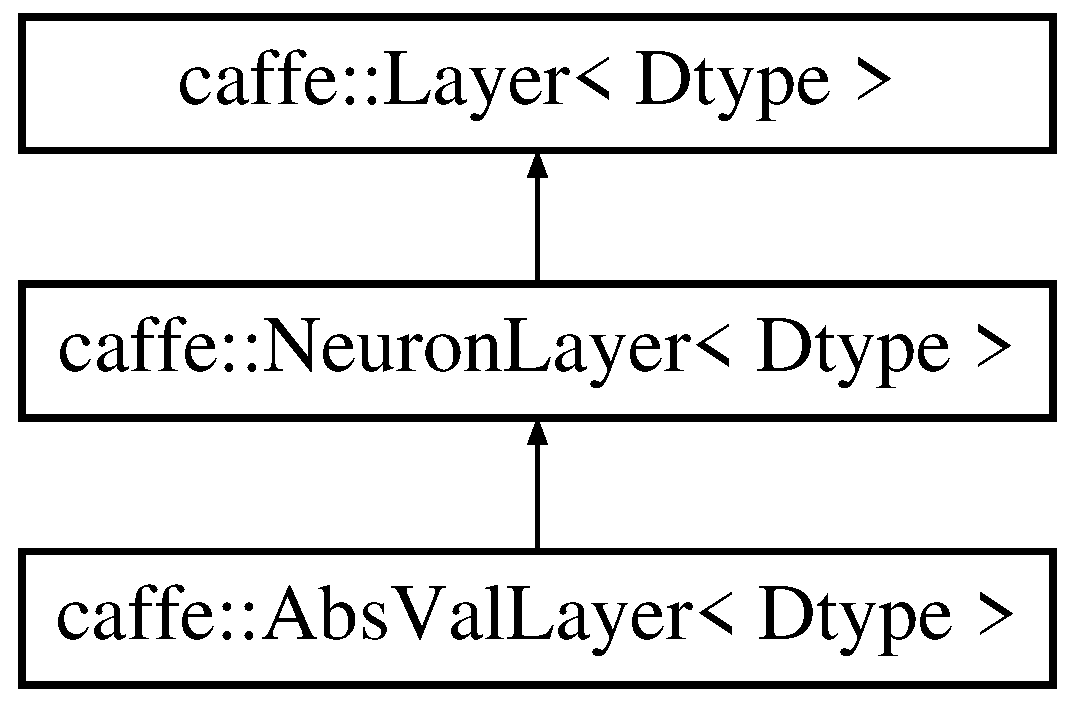
\includegraphics[height=3.000000cm]{classcaffe_1_1AbsValLayer}
\end{center}
\end{figure}
\subsection*{Public Member Functions}
\begin{DoxyCompactItemize}
\item 
{\bfseries Abs\+Val\+Layer} (const Layer\+Parameter \&param)\hypertarget{classcaffe_1_1AbsValLayer_a513c13552694e5860b85986b94793eb0}{}\label{classcaffe_1_1AbsValLayer_a513c13552694e5860b85986b94793eb0}

\item 
virtual void \hyperlink{classcaffe_1_1AbsValLayer_acfb0677a17e9d3b4920ff62d3b0d800a}{Layer\+Set\+Up} (const vector$<$ \hyperlink{classcaffe_1_1Blob}{Blob}$<$ Dtype $>$ $\ast$ $>$ \&bottom, const vector$<$ \hyperlink{classcaffe_1_1Blob}{Blob}$<$ Dtype $>$ $\ast$ $>$ \&top)
\begin{DoxyCompactList}\small\item\em Does layer-\/specific setup\+: your layer should implement this function as well as Reshape. \end{DoxyCompactList}\item 
virtual const char $\ast$ \hyperlink{classcaffe_1_1AbsValLayer_a35f8a7f7ae11e115f5bd5dac67abf555}{type} () const \hypertarget{classcaffe_1_1AbsValLayer_a35f8a7f7ae11e115f5bd5dac67abf555}{}\label{classcaffe_1_1AbsValLayer_a35f8a7f7ae11e115f5bd5dac67abf555}

\begin{DoxyCompactList}\small\item\em Returns the layer type. \end{DoxyCompactList}\item 
virtual int \hyperlink{classcaffe_1_1AbsValLayer_a0e797616508e76aa9c2ce19a1b08dff0}{Exact\+Num\+Bottom\+Blobs} () const 
\begin{DoxyCompactList}\small\item\em Returns the exact number of bottom blobs required by the layer, or -\/1 if no exact number is required. \end{DoxyCompactList}\item 
virtual int \hyperlink{classcaffe_1_1AbsValLayer_abddadbf826dc2ffaf22738804a484208}{Exact\+Num\+Top\+Blobs} () const 
\begin{DoxyCompactList}\small\item\em Returns the exact number of top blobs required by the layer, or -\/1 if no exact number is required. \end{DoxyCompactList}\end{DoxyCompactItemize}
\subsection*{Protected Member Functions}
\begin{DoxyCompactItemize}
\item 
virtual void \hyperlink{classcaffe_1_1AbsValLayer_a6f9bc11e2459c982b44482305390dfc7}{Forward\+\_\+cpu} (const vector$<$ \hyperlink{classcaffe_1_1Blob}{Blob}$<$ Dtype $>$ $\ast$ $>$ \&bottom, const vector$<$ \hyperlink{classcaffe_1_1Blob}{Blob}$<$ Dtype $>$ $\ast$ $>$ \&top)
\begin{DoxyCompactList}\small\item\em Computes $ y = |x| $. \end{DoxyCompactList}\item 
virtual void \hyperlink{classcaffe_1_1AbsValLayer_abe4da39f8844524e745a92d9766adccc}{Forward\+\_\+gpu} (const vector$<$ \hyperlink{classcaffe_1_1Blob}{Blob}$<$ Dtype $>$ $\ast$ $>$ \&bottom, const vector$<$ \hyperlink{classcaffe_1_1Blob}{Blob}$<$ Dtype $>$ $\ast$ $>$ \&top)\hypertarget{classcaffe_1_1AbsValLayer_abe4da39f8844524e745a92d9766adccc}{}\label{classcaffe_1_1AbsValLayer_abe4da39f8844524e745a92d9766adccc}

\begin{DoxyCompactList}\small\item\em Using the G\+PU device, compute the layer output. Fall back to \hyperlink{classcaffe_1_1AbsValLayer_a6f9bc11e2459c982b44482305390dfc7}{Forward\+\_\+cpu()} if unavailable. \end{DoxyCompactList}\item 
virtual void \hyperlink{classcaffe_1_1AbsValLayer_a1d81dee85d0f354986e0f6f984974599}{Backward\+\_\+cpu} (const vector$<$ \hyperlink{classcaffe_1_1Blob}{Blob}$<$ Dtype $>$ $\ast$ $>$ \&top, const vector$<$ bool $>$ \&propagate\+\_\+down, const vector$<$ \hyperlink{classcaffe_1_1Blob}{Blob}$<$ Dtype $>$ $\ast$ $>$ \&bottom)
\begin{DoxyCompactList}\small\item\em Computes the error gradient w.\+r.\+t. the absolute value inputs. \end{DoxyCompactList}\item 
virtual void \hyperlink{classcaffe_1_1AbsValLayer_a9dfa072afd31d0261763074be0a797ec}{Backward\+\_\+gpu} (const vector$<$ \hyperlink{classcaffe_1_1Blob}{Blob}$<$ Dtype $>$ $\ast$ $>$ \&top, const vector$<$ bool $>$ \&propagate\+\_\+down, const vector$<$ \hyperlink{classcaffe_1_1Blob}{Blob}$<$ Dtype $>$ $\ast$ $>$ \&bottom)\hypertarget{classcaffe_1_1AbsValLayer_a9dfa072afd31d0261763074be0a797ec}{}\label{classcaffe_1_1AbsValLayer_a9dfa072afd31d0261763074be0a797ec}

\begin{DoxyCompactList}\small\item\em Using the G\+PU device, compute the gradients for any parameters and for the bottom blobs if propagate\+\_\+down is true. Fall back to \hyperlink{classcaffe_1_1AbsValLayer_a1d81dee85d0f354986e0f6f984974599}{Backward\+\_\+cpu()} if unavailable. \end{DoxyCompactList}\end{DoxyCompactItemize}
\subsection*{Additional Inherited Members}


\subsection{Detailed Description}
\subsubsection*{template$<$typename Dtype$>$\\*
class caffe\+::\+Abs\+Val\+Layer$<$ Dtype $>$}

Computes $ y = |x| $. 


\begin{DoxyParams}{Parameters}
{\em bottom} & input \hyperlink{classcaffe_1_1Blob}{Blob} vector (length 1)
\begin{DoxyEnumerate}
\item $ (N \times C \times H \times W) $ the inputs $ x $ 
\end{DoxyEnumerate}\\
\hline
{\em top} & output \hyperlink{classcaffe_1_1Blob}{Blob} vector (length 1)
\begin{DoxyEnumerate}
\item $ (N \times C \times H \times W) $ the computed outputs $ y = |x| $ 
\end{DoxyEnumerate}\\
\hline
\end{DoxyParams}


\subsection{Member Function Documentation}
\index{caffe\+::\+Abs\+Val\+Layer@{caffe\+::\+Abs\+Val\+Layer}!Backward\+\_\+cpu@{Backward\+\_\+cpu}}
\index{Backward\+\_\+cpu@{Backward\+\_\+cpu}!caffe\+::\+Abs\+Val\+Layer@{caffe\+::\+Abs\+Val\+Layer}}
\subsubsection[{\texorpdfstring{Backward\+\_\+cpu(const vector$<$ Blob$<$ Dtype $>$ $\ast$ $>$ \&top, const vector$<$ bool $>$ \&propagate\+\_\+down, const vector$<$ Blob$<$ Dtype $>$ $\ast$ $>$ \&bottom)}{Backward_cpu(const vector< Blob< Dtype > * > &top, const vector< bool > &propagate_down, const vector< Blob< Dtype > * > &bottom)}}]{\setlength{\rightskip}{0pt plus 5cm}template$<$typename Dtype $>$ void {\bf caffe\+::\+Abs\+Val\+Layer}$<$ Dtype $>$\+::Backward\+\_\+cpu (
\begin{DoxyParamCaption}
\item[{const vector$<$ {\bf Blob}$<$ Dtype $>$ $\ast$ $>$ \&}]{top, }
\item[{const vector$<$ bool $>$ \&}]{propagate\+\_\+down, }
\item[{const vector$<$ {\bf Blob}$<$ Dtype $>$ $\ast$ $>$ \&}]{bottom}
\end{DoxyParamCaption}
)\hspace{0.3cm}{\ttfamily [protected]}, {\ttfamily [virtual]}}\hypertarget{classcaffe_1_1AbsValLayer_a1d81dee85d0f354986e0f6f984974599}{}\label{classcaffe_1_1AbsValLayer_a1d81dee85d0f354986e0f6f984974599}


Computes the error gradient w.\+r.\+t. the absolute value inputs. 


\begin{DoxyParams}{Parameters}
{\em top} & output \hyperlink{classcaffe_1_1Blob}{Blob} vector (length 1), providing the error gradient with respect to the outputs
\begin{DoxyEnumerate}
\item $ (N \times C \times H \times W) $ containing error gradients $ \frac{\partial E}{\partial y} $ with respect to computed outputs $ y $ 
\end{DoxyEnumerate}\\
\hline
{\em propagate\+\_\+down} & see \hyperlink{classcaffe_1_1Layer_a53df1e081767e07bfb4c81657f4acd0a}{Layer\+::\+Backward}. \\
\hline
{\em bottom} & input \hyperlink{classcaffe_1_1Blob}{Blob} vector (length 2)
\begin{DoxyEnumerate}
\item $ (N \times C \times H \times W) $ the inputs $ x $; Backward fills their diff with gradients $ \frac{\partial E}{\partial x} = \mathrm{sign}(x) \frac{\partial E}{\partial y} $ if propagate\+\_\+down\mbox{[}0\mbox{]} 
\end{DoxyEnumerate}\\
\hline
\end{DoxyParams}


Implements \hyperlink{classcaffe_1_1Layer_a64d15855f882af4b82e83fa993c4e7c6}{caffe\+::\+Layer$<$ Dtype $>$}.

\index{caffe\+::\+Abs\+Val\+Layer@{caffe\+::\+Abs\+Val\+Layer}!Exact\+Num\+Bottom\+Blobs@{Exact\+Num\+Bottom\+Blobs}}
\index{Exact\+Num\+Bottom\+Blobs@{Exact\+Num\+Bottom\+Blobs}!caffe\+::\+Abs\+Val\+Layer@{caffe\+::\+Abs\+Val\+Layer}}
\subsubsection[{\texorpdfstring{Exact\+Num\+Bottom\+Blobs() const }{ExactNumBottomBlobs() const }}]{\setlength{\rightskip}{0pt plus 5cm}template$<$typename Dtype $>$ virtual int {\bf caffe\+::\+Abs\+Val\+Layer}$<$ Dtype $>$\+::Exact\+Num\+Bottom\+Blobs (
\begin{DoxyParamCaption}
{}
\end{DoxyParamCaption}
) const\hspace{0.3cm}{\ttfamily [inline]}, {\ttfamily [virtual]}}\hypertarget{classcaffe_1_1AbsValLayer_a0e797616508e76aa9c2ce19a1b08dff0}{}\label{classcaffe_1_1AbsValLayer_a0e797616508e76aa9c2ce19a1b08dff0}


Returns the exact number of bottom blobs required by the layer, or -\/1 if no exact number is required. 

This method should be overridden to return a non-\/negative value if your layer expects some exact number of bottom blobs. 

Reimplemented from \hyperlink{classcaffe_1_1NeuronLayer_a83678ec7f661054d36d83fa062b639b2}{caffe\+::\+Neuron\+Layer$<$ Dtype $>$}.

\index{caffe\+::\+Abs\+Val\+Layer@{caffe\+::\+Abs\+Val\+Layer}!Exact\+Num\+Top\+Blobs@{Exact\+Num\+Top\+Blobs}}
\index{Exact\+Num\+Top\+Blobs@{Exact\+Num\+Top\+Blobs}!caffe\+::\+Abs\+Val\+Layer@{caffe\+::\+Abs\+Val\+Layer}}
\subsubsection[{\texorpdfstring{Exact\+Num\+Top\+Blobs() const }{ExactNumTopBlobs() const }}]{\setlength{\rightskip}{0pt plus 5cm}template$<$typename Dtype $>$ virtual int {\bf caffe\+::\+Abs\+Val\+Layer}$<$ Dtype $>$\+::Exact\+Num\+Top\+Blobs (
\begin{DoxyParamCaption}
{}
\end{DoxyParamCaption}
) const\hspace{0.3cm}{\ttfamily [inline]}, {\ttfamily [virtual]}}\hypertarget{classcaffe_1_1AbsValLayer_abddadbf826dc2ffaf22738804a484208}{}\label{classcaffe_1_1AbsValLayer_abddadbf826dc2ffaf22738804a484208}


Returns the exact number of top blobs required by the layer, or -\/1 if no exact number is required. 

This method should be overridden to return a non-\/negative value if your layer expects some exact number of top blobs. 

Reimplemented from \hyperlink{classcaffe_1_1NeuronLayer_a25dfa84e8b46705aa7a822e734b4f04f}{caffe\+::\+Neuron\+Layer$<$ Dtype $>$}.

\index{caffe\+::\+Abs\+Val\+Layer@{caffe\+::\+Abs\+Val\+Layer}!Forward\+\_\+cpu@{Forward\+\_\+cpu}}
\index{Forward\+\_\+cpu@{Forward\+\_\+cpu}!caffe\+::\+Abs\+Val\+Layer@{caffe\+::\+Abs\+Val\+Layer}}
\subsubsection[{\texorpdfstring{Forward\+\_\+cpu(const vector$<$ Blob$<$ Dtype $>$ $\ast$ $>$ \&bottom, const vector$<$ Blob$<$ Dtype $>$ $\ast$ $>$ \&top)}{Forward_cpu(const vector< Blob< Dtype > * > &bottom, const vector< Blob< Dtype > * > &top)}}]{\setlength{\rightskip}{0pt plus 5cm}template$<$typename Dtype $>$ void {\bf caffe\+::\+Abs\+Val\+Layer}$<$ Dtype $>$\+::Forward\+\_\+cpu (
\begin{DoxyParamCaption}
\item[{const vector$<$ {\bf Blob}$<$ Dtype $>$ $\ast$ $>$ \&}]{bottom, }
\item[{const vector$<$ {\bf Blob}$<$ Dtype $>$ $\ast$ $>$ \&}]{top}
\end{DoxyParamCaption}
)\hspace{0.3cm}{\ttfamily [protected]}, {\ttfamily [virtual]}}\hypertarget{classcaffe_1_1AbsValLayer_a6f9bc11e2459c982b44482305390dfc7}{}\label{classcaffe_1_1AbsValLayer_a6f9bc11e2459c982b44482305390dfc7}


Computes $ y = |x| $. 


\begin{DoxyParams}{Parameters}
{\em bottom} & input \hyperlink{classcaffe_1_1Blob}{Blob} vector (length 1)
\begin{DoxyEnumerate}
\item $ (N \times C \times H \times W) $ the inputs $ x $ 
\end{DoxyEnumerate}\\
\hline
{\em top} & output \hyperlink{classcaffe_1_1Blob}{Blob} vector (length 1)
\begin{DoxyEnumerate}
\item $ (N \times C \times H \times W) $ the computed outputs $ y = |x| $ 
\end{DoxyEnumerate}\\
\hline
\end{DoxyParams}


Implements \hyperlink{classcaffe_1_1Layer_add965883f75bbf90c7a06f960cda7a1a}{caffe\+::\+Layer$<$ Dtype $>$}.

\index{caffe\+::\+Abs\+Val\+Layer@{caffe\+::\+Abs\+Val\+Layer}!Layer\+Set\+Up@{Layer\+Set\+Up}}
\index{Layer\+Set\+Up@{Layer\+Set\+Up}!caffe\+::\+Abs\+Val\+Layer@{caffe\+::\+Abs\+Val\+Layer}}
\subsubsection[{\texorpdfstring{Layer\+Set\+Up(const vector$<$ Blob$<$ Dtype $>$ $\ast$ $>$ \&bottom, const vector$<$ Blob$<$ Dtype $>$ $\ast$ $>$ \&top)}{LayerSetUp(const vector< Blob< Dtype > * > &bottom, const vector< Blob< Dtype > * > &top)}}]{\setlength{\rightskip}{0pt plus 5cm}template$<$typename Dtype $>$ void {\bf caffe\+::\+Abs\+Val\+Layer}$<$ Dtype $>$\+::Layer\+Set\+Up (
\begin{DoxyParamCaption}
\item[{const vector$<$ {\bf Blob}$<$ Dtype $>$ $\ast$ $>$ \&}]{bottom, }
\item[{const vector$<$ {\bf Blob}$<$ Dtype $>$ $\ast$ $>$ \&}]{top}
\end{DoxyParamCaption}
)\hspace{0.3cm}{\ttfamily [virtual]}}\hypertarget{classcaffe_1_1AbsValLayer_acfb0677a17e9d3b4920ff62d3b0d800a}{}\label{classcaffe_1_1AbsValLayer_acfb0677a17e9d3b4920ff62d3b0d800a}


Does layer-\/specific setup\+: your layer should implement this function as well as Reshape. 


\begin{DoxyParams}{Parameters}
{\em bottom} & the preshaped input blobs, whose data fields store the input data for this layer \\
\hline
{\em top} & the allocated but unshaped output blobs\\
\hline
\end{DoxyParams}
This method should do one-\/time layer specific setup. This includes reading and processing relevent parameters from the {\ttfamily layer\+\_\+param\+\_\+}. Setting up the shapes of top blobs and internal buffers should be done in {\ttfamily Reshape}, which will be called before the forward pass to adjust the top blob sizes. 

Reimplemented from \hyperlink{classcaffe_1_1Layer_a38dc2488bf319b8de5a7ac84e0045393}{caffe\+::\+Layer$<$ Dtype $>$}.



The documentation for this class was generated from the following files\+:\begin{DoxyCompactItemize}
\item 
include/caffe/layers/absval\+\_\+layer.\+hpp\item 
src/caffe/layers/absval\+\_\+layer.\+cpp\end{DoxyCompactItemize}

\hypertarget{classcaffe_1_1AccuracyLayer}{}\section{caffe\+:\+:Accuracy\+Layer$<$ Dtype $>$ Class Template Reference}
\label{classcaffe_1_1AccuracyLayer}\index{caffe\+::\+Accuracy\+Layer$<$ Dtype $>$@{caffe\+::\+Accuracy\+Layer$<$ Dtype $>$}}


Computes the classification accuracy for a one-\/of-\/many classification task.  




{\ttfamily \#include $<$accuracy\+\_\+layer.\+hpp$>$}

Inheritance diagram for caffe\+:\+:Accuracy\+Layer$<$ Dtype $>$\+:\begin{figure}[H]
\begin{center}
\leavevmode
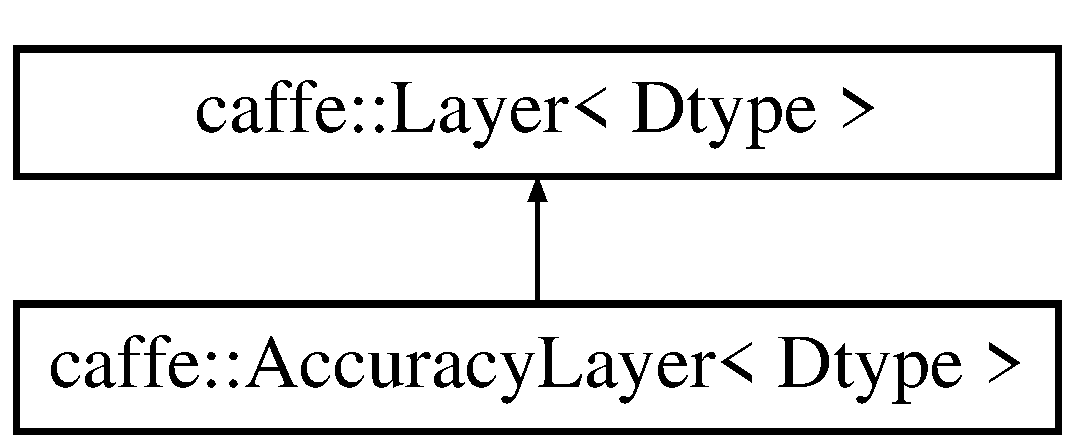
\includegraphics[height=2.000000cm]{classcaffe_1_1AccuracyLayer}
\end{center}
\end{figure}
\subsection*{Public Member Functions}
\begin{DoxyCompactItemize}
\item 
\hyperlink{classcaffe_1_1AccuracyLayer_a362ab61d1961c1b408f84a956f6e598d}{Accuracy\+Layer} (const Layer\+Parameter \&param)
\item 
virtual void \hyperlink{classcaffe_1_1AccuracyLayer_aa4e6baa79f0c23308c39be3fe5085971}{Layer\+Set\+Up} (const vector$<$ \hyperlink{classcaffe_1_1Blob}{Blob}$<$ Dtype $>$ $\ast$ $>$ \&bottom, const vector$<$ \hyperlink{classcaffe_1_1Blob}{Blob}$<$ Dtype $>$ $\ast$ $>$ \&top)
\begin{DoxyCompactList}\small\item\em Does layer-\/specific setup\+: your layer should implement this function as well as Reshape. \end{DoxyCompactList}\item 
virtual void \hyperlink{classcaffe_1_1AccuracyLayer_a28df0e6104cffdc50325a7b4d648dfa5}{Reshape} (const vector$<$ \hyperlink{classcaffe_1_1Blob}{Blob}$<$ Dtype $>$ $\ast$ $>$ \&bottom, const vector$<$ \hyperlink{classcaffe_1_1Blob}{Blob}$<$ Dtype $>$ $\ast$ $>$ \&top)
\begin{DoxyCompactList}\small\item\em Adjust the shapes of top blobs and internal buffers to accommodate the shapes of the bottom blobs. \end{DoxyCompactList}\item 
virtual const char $\ast$ \hyperlink{classcaffe_1_1AccuracyLayer_a57f6e7e7e9567cb17d9e6ae38d372091}{type} () const \hypertarget{classcaffe_1_1AccuracyLayer_a57f6e7e7e9567cb17d9e6ae38d372091}{}\label{classcaffe_1_1AccuracyLayer_a57f6e7e7e9567cb17d9e6ae38d372091}

\begin{DoxyCompactList}\small\item\em Returns the layer type. \end{DoxyCompactList}\item 
virtual int \hyperlink{classcaffe_1_1AccuracyLayer_afcde815835ab4cdf76fbbef610491a91}{Exact\+Num\+Bottom\+Blobs} () const 
\begin{DoxyCompactList}\small\item\em Returns the exact number of bottom blobs required by the layer, or -\/1 if no exact number is required. \end{DoxyCompactList}\item 
virtual int \hyperlink{classcaffe_1_1AccuracyLayer_aab0fa80d793130102ed7283ec3e41ad6}{Min\+Top\+Blobs} () const 
\begin{DoxyCompactList}\small\item\em Returns the minimum number of top blobs required by the layer, or -\/1 if no minimum number is required. \end{DoxyCompactList}\item 
virtual int \hyperlink{classcaffe_1_1AccuracyLayer_abf0eae8c25f73a302c35a9ce7b6d5544}{Max\+Top\+Blobs} () const 
\begin{DoxyCompactList}\small\item\em Returns the maximum number of top blobs required by the layer, or -\/1 if no maximum number is required. \end{DoxyCompactList}\end{DoxyCompactItemize}
\subsection*{Protected Member Functions}
\begin{DoxyCompactItemize}
\item 
virtual void \hyperlink{classcaffe_1_1AccuracyLayer_a8f7719cdffb48b7e48c29a89131f85b6}{Forward\+\_\+cpu} (const vector$<$ \hyperlink{classcaffe_1_1Blob}{Blob}$<$ Dtype $>$ $\ast$ $>$ \&bottom, const vector$<$ \hyperlink{classcaffe_1_1Blob}{Blob}$<$ Dtype $>$ $\ast$ $>$ \&top)
\item 
virtual void \hyperlink{classcaffe_1_1AccuracyLayer_a0c27449b74f79bcd9dfb5dd877c8cfdf}{Forward\+\_\+gpu} (const vector$<$ \hyperlink{classcaffe_1_1Blob}{Blob}$<$ Dtype $>$ $\ast$ $>$ \&bottom, const vector$<$ \hyperlink{classcaffe_1_1Blob}{Blob}$<$ Dtype $>$ $\ast$ $>$ \&top)\hypertarget{classcaffe_1_1AccuracyLayer_a0c27449b74f79bcd9dfb5dd877c8cfdf}{}\label{classcaffe_1_1AccuracyLayer_a0c27449b74f79bcd9dfb5dd877c8cfdf}

\begin{DoxyCompactList}\small\item\em Using the G\+PU device, compute the layer output. Fall back to \hyperlink{classcaffe_1_1AccuracyLayer_a8f7719cdffb48b7e48c29a89131f85b6}{Forward\+\_\+cpu()} if unavailable. \end{DoxyCompactList}\item 
virtual void \hyperlink{classcaffe_1_1AccuracyLayer_a1bf798e77b5dc7cd4e65e9e07ea71dac}{Backward\+\_\+cpu} (const vector$<$ \hyperlink{classcaffe_1_1Blob}{Blob}$<$ Dtype $>$ $\ast$ $>$ \&top, const vector$<$ bool $>$ \&propagate\+\_\+down, const vector$<$ \hyperlink{classcaffe_1_1Blob}{Blob}$<$ Dtype $>$ $\ast$ $>$ \&bottom)\hypertarget{classcaffe_1_1AccuracyLayer_a1bf798e77b5dc7cd4e65e9e07ea71dac}{}\label{classcaffe_1_1AccuracyLayer_a1bf798e77b5dc7cd4e65e9e07ea71dac}

\begin{DoxyCompactList}\small\item\em Not implemented -- \hyperlink{classcaffe_1_1AccuracyLayer}{Accuracy\+Layer} cannot be used as a loss. \end{DoxyCompactList}\item 
virtual void \hyperlink{classcaffe_1_1AccuracyLayer_a19e1b977ebd70b5330ed91188a1fc37d}{Backward\+\_\+gpu} (const vector$<$ \hyperlink{classcaffe_1_1Blob}{Blob}$<$ Dtype $>$ $\ast$ $>$ \&top, const vector$<$ bool $>$ \&propagate\+\_\+down, const vector$<$ \hyperlink{classcaffe_1_1Blob}{Blob}$<$ Dtype $>$ $\ast$ $>$ \&bottom)\hypertarget{classcaffe_1_1AccuracyLayer_a19e1b977ebd70b5330ed91188a1fc37d}{}\label{classcaffe_1_1AccuracyLayer_a19e1b977ebd70b5330ed91188a1fc37d}

\begin{DoxyCompactList}\small\item\em Using the G\+PU device, compute the gradients for any parameters and for the bottom blobs if propagate\+\_\+down is true. Fall back to \hyperlink{classcaffe_1_1AccuracyLayer_a1bf798e77b5dc7cd4e65e9e07ea71dac}{Backward\+\_\+cpu()} if unavailable. \end{DoxyCompactList}\end{DoxyCompactItemize}
\subsection*{Protected Attributes}
\begin{DoxyCompactItemize}
\item 
int {\bfseries label\+\_\+axis\+\_\+}\hypertarget{classcaffe_1_1AccuracyLayer_aafbbed754511b427a65d9f95707e9455}{}\label{classcaffe_1_1AccuracyLayer_aafbbed754511b427a65d9f95707e9455}

\item 
int {\bfseries outer\+\_\+num\+\_\+}\hypertarget{classcaffe_1_1AccuracyLayer_a374b3c8ce90238ec1769abf1b3b3f748}{}\label{classcaffe_1_1AccuracyLayer_a374b3c8ce90238ec1769abf1b3b3f748}

\item 
int {\bfseries inner\+\_\+num\+\_\+}\hypertarget{classcaffe_1_1AccuracyLayer_aede524eb7411cc81e3d5e62a34e96a4d}{}\label{classcaffe_1_1AccuracyLayer_aede524eb7411cc81e3d5e62a34e96a4d}

\item 
int {\bfseries top\+\_\+k\+\_\+}\hypertarget{classcaffe_1_1AccuracyLayer_a1048e10c5a499ace931cbafb9cd790d9}{}\label{classcaffe_1_1AccuracyLayer_a1048e10c5a499ace931cbafb9cd790d9}

\item 
bool \hyperlink{classcaffe_1_1AccuracyLayer_a4acdfaf6db79fbe1983b8439391ad15e}{has\+\_\+ignore\+\_\+label\+\_\+}\hypertarget{classcaffe_1_1AccuracyLayer_a4acdfaf6db79fbe1983b8439391ad15e}{}\label{classcaffe_1_1AccuracyLayer_a4acdfaf6db79fbe1983b8439391ad15e}

\begin{DoxyCompactList}\small\item\em Whether to ignore instances with a certain label. \end{DoxyCompactList}\item 
int \hyperlink{classcaffe_1_1AccuracyLayer_a2b8c2d647f43ffd6aa14e81f1c5b2bde}{ignore\+\_\+label\+\_\+}\hypertarget{classcaffe_1_1AccuracyLayer_a2b8c2d647f43ffd6aa14e81f1c5b2bde}{}\label{classcaffe_1_1AccuracyLayer_a2b8c2d647f43ffd6aa14e81f1c5b2bde}

\begin{DoxyCompactList}\small\item\em The label indicating that an instance should be ignored. \end{DoxyCompactList}\item 
\hyperlink{classcaffe_1_1Blob}{Blob}$<$ Dtype $>$ \hyperlink{classcaffe_1_1AccuracyLayer_a9acf4fa826e787fe64a55bcd2c62e66c}{nums\+\_\+buffer\+\_\+}\hypertarget{classcaffe_1_1AccuracyLayer_a9acf4fa826e787fe64a55bcd2c62e66c}{}\label{classcaffe_1_1AccuracyLayer_a9acf4fa826e787fe64a55bcd2c62e66c}

\begin{DoxyCompactList}\small\item\em Keeps counts of the number of samples per class. \end{DoxyCompactList}\end{DoxyCompactItemize}


\subsection{Detailed Description}
\subsubsection*{template$<$typename Dtype$>$\\*
class caffe\+::\+Accuracy\+Layer$<$ Dtype $>$}

Computes the classification accuracy for a one-\/of-\/many classification task. 

\subsection{Constructor \& Destructor Documentation}
\index{caffe\+::\+Accuracy\+Layer@{caffe\+::\+Accuracy\+Layer}!Accuracy\+Layer@{Accuracy\+Layer}}
\index{Accuracy\+Layer@{Accuracy\+Layer}!caffe\+::\+Accuracy\+Layer@{caffe\+::\+Accuracy\+Layer}}
\subsubsection[{\texorpdfstring{Accuracy\+Layer(const Layer\+Parameter \&param)}{AccuracyLayer(const LayerParameter &param)}}]{\setlength{\rightskip}{0pt plus 5cm}template$<$typename Dtype $>$ {\bf caffe\+::\+Accuracy\+Layer}$<$ Dtype $>$\+::{\bf Accuracy\+Layer} (
\begin{DoxyParamCaption}
\item[{const Layer\+Parameter \&}]{param}
\end{DoxyParamCaption}
)\hspace{0.3cm}{\ttfamily [inline]}, {\ttfamily [explicit]}}\hypertarget{classcaffe_1_1AccuracyLayer_a362ab61d1961c1b408f84a956f6e598d}{}\label{classcaffe_1_1AccuracyLayer_a362ab61d1961c1b408f84a956f6e598d}

\begin{DoxyParams}{Parameters}
{\em param} & provides Accuracy\+Parameter accuracy\+\_\+param, with \hyperlink{classcaffe_1_1AccuracyLayer}{Accuracy\+Layer} options\+:
\begin{DoxyItemize}
\item top\+\_\+k ({\bfseries optional}, default 1). Sets the maximum rank $ k $ at which a prediction is considered correct. For example, if $ k = 5 $, a prediction is counted correct if the correct label is among the top 5 predicted labels. 
\end{DoxyItemize}\\
\hline
\end{DoxyParams}


\subsection{Member Function Documentation}
\index{caffe\+::\+Accuracy\+Layer@{caffe\+::\+Accuracy\+Layer}!Exact\+Num\+Bottom\+Blobs@{Exact\+Num\+Bottom\+Blobs}}
\index{Exact\+Num\+Bottom\+Blobs@{Exact\+Num\+Bottom\+Blobs}!caffe\+::\+Accuracy\+Layer@{caffe\+::\+Accuracy\+Layer}}
\subsubsection[{\texorpdfstring{Exact\+Num\+Bottom\+Blobs() const }{ExactNumBottomBlobs() const }}]{\setlength{\rightskip}{0pt plus 5cm}template$<$typename Dtype $>$ virtual int {\bf caffe\+::\+Accuracy\+Layer}$<$ Dtype $>$\+::Exact\+Num\+Bottom\+Blobs (
\begin{DoxyParamCaption}
{}
\end{DoxyParamCaption}
) const\hspace{0.3cm}{\ttfamily [inline]}, {\ttfamily [virtual]}}\hypertarget{classcaffe_1_1AccuracyLayer_afcde815835ab4cdf76fbbef610491a91}{}\label{classcaffe_1_1AccuracyLayer_afcde815835ab4cdf76fbbef610491a91}


Returns the exact number of bottom blobs required by the layer, or -\/1 if no exact number is required. 

This method should be overridden to return a non-\/negative value if your layer expects some exact number of bottom blobs. 

Reimplemented from \hyperlink{classcaffe_1_1Layer_a45c7a7943a8a6735ac433c9be11e0240}{caffe\+::\+Layer$<$ Dtype $>$}.

\index{caffe\+::\+Accuracy\+Layer@{caffe\+::\+Accuracy\+Layer}!Forward\+\_\+cpu@{Forward\+\_\+cpu}}
\index{Forward\+\_\+cpu@{Forward\+\_\+cpu}!caffe\+::\+Accuracy\+Layer@{caffe\+::\+Accuracy\+Layer}}
\subsubsection[{\texorpdfstring{Forward\+\_\+cpu(const vector$<$ Blob$<$ Dtype $>$ $\ast$ $>$ \&bottom, const vector$<$ Blob$<$ Dtype $>$ $\ast$ $>$ \&top)}{Forward_cpu(const vector< Blob< Dtype > * > &bottom, const vector< Blob< Dtype > * > &top)}}]{\setlength{\rightskip}{0pt plus 5cm}template$<$typename Dtype $>$ void {\bf caffe\+::\+Accuracy\+Layer}$<$ Dtype $>$\+::Forward\+\_\+cpu (
\begin{DoxyParamCaption}
\item[{const vector$<$ {\bf Blob}$<$ Dtype $>$ $\ast$ $>$ \&}]{bottom, }
\item[{const vector$<$ {\bf Blob}$<$ Dtype $>$ $\ast$ $>$ \&}]{top}
\end{DoxyParamCaption}
)\hspace{0.3cm}{\ttfamily [protected]}, {\ttfamily [virtual]}}\hypertarget{classcaffe_1_1AccuracyLayer_a8f7719cdffb48b7e48c29a89131f85b6}{}\label{classcaffe_1_1AccuracyLayer_a8f7719cdffb48b7e48c29a89131f85b6}

\begin{DoxyParams}{Parameters}
{\em bottom} & input \hyperlink{classcaffe_1_1Blob}{Blob} vector (length 2)
\begin{DoxyEnumerate}
\item $ (N \times C \times H \times W) $ the predictions $ x $, a \hyperlink{classcaffe_1_1Blob}{Blob} with values in $ [-\infty, +\infty] $ indicating the predicted score for each of the $ K = CHW $ classes. Each $ x_n $ is mapped to a predicted label $ \hat{l}_n $ given by its maximal index\+: $ \hat{l}_n = \arg\max\limits_k x_{nk} $
\item $ (N \times 1 \times 1 \times 1) $ the labels $ l $, an integer-\/valued \hyperlink{classcaffe_1_1Blob}{Blob} with values $ l_n \in [0, 1, 2, ..., K - 1] $ indicating the correct class label among the $ K $ classes 
\end{DoxyEnumerate}\\
\hline
{\em top} & output \hyperlink{classcaffe_1_1Blob}{Blob} vector (length 1)
\begin{DoxyEnumerate}
\item $ (1 \times 1 \times 1 \times 1) $ the computed accuracy\+: $ \frac{1}{N} \sum\limits_{n=1}^N \delta\{ \hat{l}_n = l_n \} $, where $ \delta\{\mathrm{condition}\} = \left\{ \begin{array}{lr} 1 & \mbox{if condition} \\ 0 & \mbox{otherwise} \end{array} \right. $ 
\end{DoxyEnumerate}\\
\hline
\end{DoxyParams}


Implements \hyperlink{classcaffe_1_1Layer_add965883f75bbf90c7a06f960cda7a1a}{caffe\+::\+Layer$<$ Dtype $>$}.

\index{caffe\+::\+Accuracy\+Layer@{caffe\+::\+Accuracy\+Layer}!Layer\+Set\+Up@{Layer\+Set\+Up}}
\index{Layer\+Set\+Up@{Layer\+Set\+Up}!caffe\+::\+Accuracy\+Layer@{caffe\+::\+Accuracy\+Layer}}
\subsubsection[{\texorpdfstring{Layer\+Set\+Up(const vector$<$ Blob$<$ Dtype $>$ $\ast$ $>$ \&bottom, const vector$<$ Blob$<$ Dtype $>$ $\ast$ $>$ \&top)}{LayerSetUp(const vector< Blob< Dtype > * > &bottom, const vector< Blob< Dtype > * > &top)}}]{\setlength{\rightskip}{0pt plus 5cm}template$<$typename Dtype $>$ void {\bf caffe\+::\+Accuracy\+Layer}$<$ Dtype $>$\+::Layer\+Set\+Up (
\begin{DoxyParamCaption}
\item[{const vector$<$ {\bf Blob}$<$ Dtype $>$ $\ast$ $>$ \&}]{bottom, }
\item[{const vector$<$ {\bf Blob}$<$ Dtype $>$ $\ast$ $>$ \&}]{top}
\end{DoxyParamCaption}
)\hspace{0.3cm}{\ttfamily [virtual]}}\hypertarget{classcaffe_1_1AccuracyLayer_aa4e6baa79f0c23308c39be3fe5085971}{}\label{classcaffe_1_1AccuracyLayer_aa4e6baa79f0c23308c39be3fe5085971}


Does layer-\/specific setup\+: your layer should implement this function as well as Reshape. 


\begin{DoxyParams}{Parameters}
{\em bottom} & the preshaped input blobs, whose data fields store the input data for this layer \\
\hline
{\em top} & the allocated but unshaped output blobs\\
\hline
\end{DoxyParams}
This method should do one-\/time layer specific setup. This includes reading and processing relevent parameters from the {\ttfamily layer\+\_\+param\+\_\+}. Setting up the shapes of top blobs and internal buffers should be done in {\ttfamily Reshape}, which will be called before the forward pass to adjust the top blob sizes. 

Reimplemented from \hyperlink{classcaffe_1_1Layer_a38dc2488bf319b8de5a7ac84e0045393}{caffe\+::\+Layer$<$ Dtype $>$}.

\index{caffe\+::\+Accuracy\+Layer@{caffe\+::\+Accuracy\+Layer}!Max\+Top\+Blobs@{Max\+Top\+Blobs}}
\index{Max\+Top\+Blobs@{Max\+Top\+Blobs}!caffe\+::\+Accuracy\+Layer@{caffe\+::\+Accuracy\+Layer}}
\subsubsection[{\texorpdfstring{Max\+Top\+Blobs() const }{MaxTopBlobs() const }}]{\setlength{\rightskip}{0pt plus 5cm}template$<$typename Dtype $>$ virtual int {\bf caffe\+::\+Accuracy\+Layer}$<$ Dtype $>$\+::Max\+Top\+Blobs (
\begin{DoxyParamCaption}
{}
\end{DoxyParamCaption}
) const\hspace{0.3cm}{\ttfamily [inline]}, {\ttfamily [virtual]}}\hypertarget{classcaffe_1_1AccuracyLayer_abf0eae8c25f73a302c35a9ce7b6d5544}{}\label{classcaffe_1_1AccuracyLayer_abf0eae8c25f73a302c35a9ce7b6d5544}


Returns the maximum number of top blobs required by the layer, or -\/1 if no maximum number is required. 

This method should be overridden to return a non-\/negative value if your layer expects some maximum number of top blobs. 

Reimplemented from \hyperlink{classcaffe_1_1Layer_adeff774663c6ec94424901d2746e2f03}{caffe\+::\+Layer$<$ Dtype $>$}.

\index{caffe\+::\+Accuracy\+Layer@{caffe\+::\+Accuracy\+Layer}!Min\+Top\+Blobs@{Min\+Top\+Blobs}}
\index{Min\+Top\+Blobs@{Min\+Top\+Blobs}!caffe\+::\+Accuracy\+Layer@{caffe\+::\+Accuracy\+Layer}}
\subsubsection[{\texorpdfstring{Min\+Top\+Blobs() const }{MinTopBlobs() const }}]{\setlength{\rightskip}{0pt plus 5cm}template$<$typename Dtype $>$ virtual int {\bf caffe\+::\+Accuracy\+Layer}$<$ Dtype $>$\+::Min\+Top\+Blobs (
\begin{DoxyParamCaption}
{}
\end{DoxyParamCaption}
) const\hspace{0.3cm}{\ttfamily [inline]}, {\ttfamily [virtual]}}\hypertarget{classcaffe_1_1AccuracyLayer_aab0fa80d793130102ed7283ec3e41ad6}{}\label{classcaffe_1_1AccuracyLayer_aab0fa80d793130102ed7283ec3e41ad6}


Returns the minimum number of top blobs required by the layer, or -\/1 if no minimum number is required. 

This method should be overridden to return a non-\/negative value if your layer expects some minimum number of top blobs. 

Reimplemented from \hyperlink{classcaffe_1_1Layer_a8bb143d58a740345fa2dc3d4204d553b}{caffe\+::\+Layer$<$ Dtype $>$}.

\index{caffe\+::\+Accuracy\+Layer@{caffe\+::\+Accuracy\+Layer}!Reshape@{Reshape}}
\index{Reshape@{Reshape}!caffe\+::\+Accuracy\+Layer@{caffe\+::\+Accuracy\+Layer}}
\subsubsection[{\texorpdfstring{Reshape(const vector$<$ Blob$<$ Dtype $>$ $\ast$ $>$ \&bottom, const vector$<$ Blob$<$ Dtype $>$ $\ast$ $>$ \&top)}{Reshape(const vector< Blob< Dtype > * > &bottom, const vector< Blob< Dtype > * > &top)}}]{\setlength{\rightskip}{0pt plus 5cm}template$<$typename Dtype $>$ void {\bf caffe\+::\+Accuracy\+Layer}$<$ Dtype $>$\+::Reshape (
\begin{DoxyParamCaption}
\item[{const vector$<$ {\bf Blob}$<$ Dtype $>$ $\ast$ $>$ \&}]{bottom, }
\item[{const vector$<$ {\bf Blob}$<$ Dtype $>$ $\ast$ $>$ \&}]{top}
\end{DoxyParamCaption}
)\hspace{0.3cm}{\ttfamily [virtual]}}\hypertarget{classcaffe_1_1AccuracyLayer_a28df0e6104cffdc50325a7b4d648dfa5}{}\label{classcaffe_1_1AccuracyLayer_a28df0e6104cffdc50325a7b4d648dfa5}


Adjust the shapes of top blobs and internal buffers to accommodate the shapes of the bottom blobs. 


\begin{DoxyParams}{Parameters}
{\em bottom} & the input blobs, with the requested input shapes \\
\hline
{\em top} & the top blobs, which should be reshaped as needed\\
\hline
\end{DoxyParams}
This method should reshape top blobs as needed according to the shapes of the bottom (input) blobs, as well as reshaping any internal buffers and making any other necessary adjustments so that the layer can accommodate the bottom blobs. 

Implements \hyperlink{classcaffe_1_1Layer_ad9d391b972c769c0ebee34ca6d1c973e}{caffe\+::\+Layer$<$ Dtype $>$}.



The documentation for this class was generated from the following files\+:\begin{DoxyCompactItemize}
\item 
include/caffe/layers/accuracy\+\_\+layer.\+hpp\item 
src/caffe/layers/accuracy\+\_\+layer.\+cpp\end{DoxyCompactItemize}

\hypertarget{classcaffe_1_1AdaDeltaSolver}{}\section{caffe\+:\+:Ada\+Delta\+Solver$<$ Dtype $>$ Class Template Reference}
\label{classcaffe_1_1AdaDeltaSolver}\index{caffe\+::\+Ada\+Delta\+Solver$<$ Dtype $>$@{caffe\+::\+Ada\+Delta\+Solver$<$ Dtype $>$}}
Inheritance diagram for caffe\+:\+:Ada\+Delta\+Solver$<$ Dtype $>$\+:\begin{figure}[H]
\begin{center}
\leavevmode
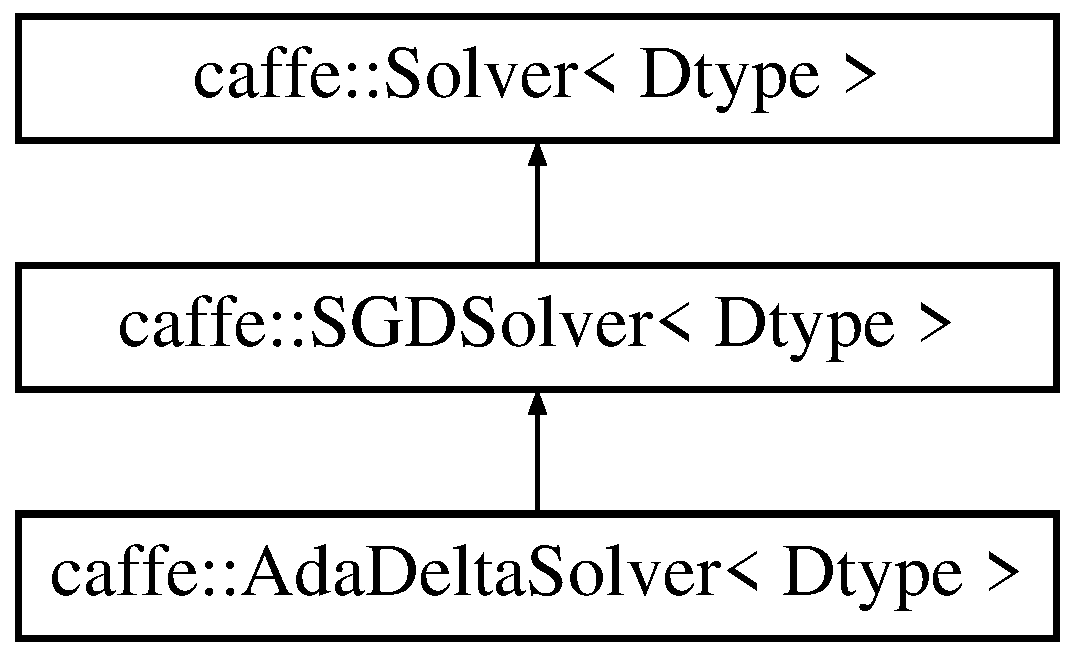
\includegraphics[height=3.000000cm]{classcaffe_1_1AdaDeltaSolver}
\end{center}
\end{figure}
\subsection*{Public Member Functions}
\begin{DoxyCompactItemize}
\item 
{\bfseries Ada\+Delta\+Solver} (const Solver\+Parameter \&param)\hypertarget{classcaffe_1_1AdaDeltaSolver_ad6f176b0beaa4a41d111f2c10a35b2f5}{}\label{classcaffe_1_1AdaDeltaSolver_ad6f176b0beaa4a41d111f2c10a35b2f5}

\item 
{\bfseries Ada\+Delta\+Solver} (const string \&param\+\_\+file)\hypertarget{classcaffe_1_1AdaDeltaSolver_adba552de0f9aa7e165cca5919d69cc09}{}\label{classcaffe_1_1AdaDeltaSolver_adba552de0f9aa7e165cca5919d69cc09}

\item 
virtual const char $\ast$ \hyperlink{classcaffe_1_1AdaDeltaSolver_a017ccdbd9a08a4b4b4db3013859a6cb0}{type} () const \hypertarget{classcaffe_1_1AdaDeltaSolver_a017ccdbd9a08a4b4b4db3013859a6cb0}{}\label{classcaffe_1_1AdaDeltaSolver_a017ccdbd9a08a4b4b4db3013859a6cb0}

\begin{DoxyCompactList}\small\item\em Returns the solver type. \end{DoxyCompactList}\end{DoxyCompactItemize}
\subsection*{Protected Member Functions}
\begin{DoxyCompactItemize}
\item 
void {\bfseries Ada\+Delta\+Pre\+Solve} ()\hypertarget{classcaffe_1_1AdaDeltaSolver_a5aae9f8d57714dd41e92c7a285d31d0a}{}\label{classcaffe_1_1AdaDeltaSolver_a5aae9f8d57714dd41e92c7a285d31d0a}

\item 
virtual void {\bfseries Compute\+Update\+Value} (int param\+\_\+id, Dtype rate)\hypertarget{classcaffe_1_1AdaDeltaSolver_aa3b649a03988cab462d411e26784f209}{}\label{classcaffe_1_1AdaDeltaSolver_aa3b649a03988cab462d411e26784f209}

\item 
{\bfseries D\+I\+S\+A\+B\+L\+E\+\_\+\+C\+O\+P\+Y\+\_\+\+A\+N\+D\+\_\+\+A\+S\+S\+I\+GN} (\hyperlink{classcaffe_1_1AdaDeltaSolver}{Ada\+Delta\+Solver})\hypertarget{classcaffe_1_1AdaDeltaSolver_ae1097650f9ae280b649d3b116c26152f}{}\label{classcaffe_1_1AdaDeltaSolver_ae1097650f9ae280b649d3b116c26152f}

\end{DoxyCompactItemize}
\subsection*{Additional Inherited Members}


The documentation for this class was generated from the following files\+:\begin{DoxyCompactItemize}
\item 
include/caffe/sgd\+\_\+solvers.\+hpp\item 
src/caffe/solvers/adadelta\+\_\+solver.\+cpp\end{DoxyCompactItemize}

\hypertarget{classcaffe_1_1AdaGradSolver}{}\section{caffe\+:\+:Ada\+Grad\+Solver$<$ Dtype $>$ Class Template Reference}
\label{classcaffe_1_1AdaGradSolver}\index{caffe\+::\+Ada\+Grad\+Solver$<$ Dtype $>$@{caffe\+::\+Ada\+Grad\+Solver$<$ Dtype $>$}}
Inheritance diagram for caffe\+:\+:Ada\+Grad\+Solver$<$ Dtype $>$\+:\begin{figure}[H]
\begin{center}
\leavevmode
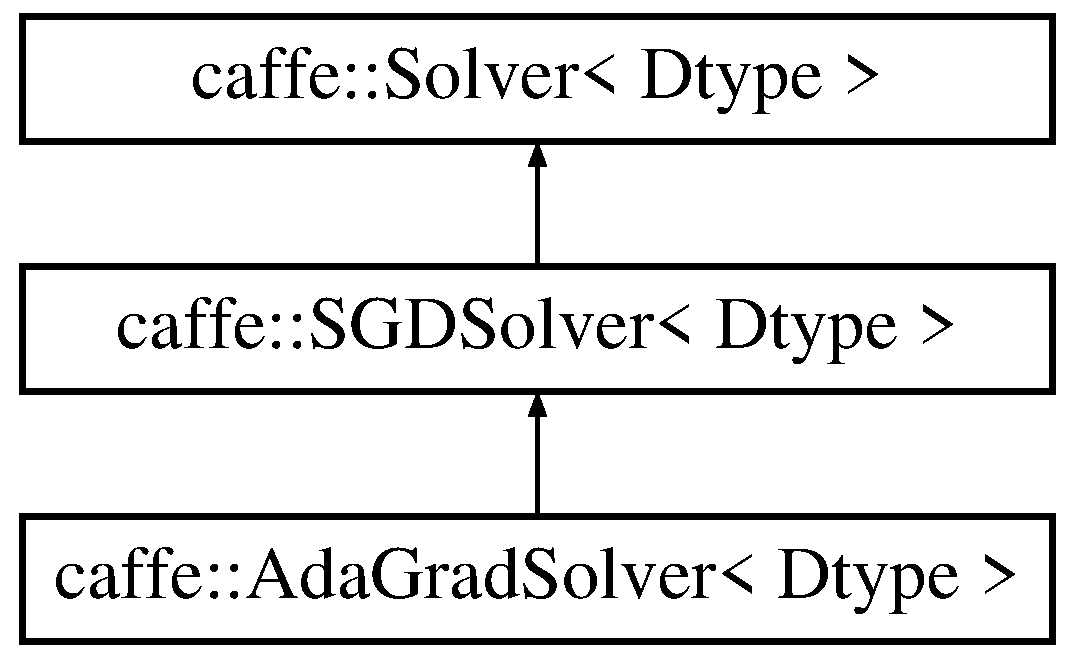
\includegraphics[height=3.000000cm]{classcaffe_1_1AdaGradSolver}
\end{center}
\end{figure}
\subsection*{Public Member Functions}
\begin{DoxyCompactItemize}
\item 
{\bfseries Ada\+Grad\+Solver} (const Solver\+Parameter \&param)\hypertarget{classcaffe_1_1AdaGradSolver_acfa678395af17eb9cfcf21e8b9fe5ce9}{}\label{classcaffe_1_1AdaGradSolver_acfa678395af17eb9cfcf21e8b9fe5ce9}

\item 
{\bfseries Ada\+Grad\+Solver} (const string \&param\+\_\+file)\hypertarget{classcaffe_1_1AdaGradSolver_aca70c4ae0d471a6a2610d371e95f5ffa}{}\label{classcaffe_1_1AdaGradSolver_aca70c4ae0d471a6a2610d371e95f5ffa}

\item 
virtual const char $\ast$ \hyperlink{classcaffe_1_1AdaGradSolver_a84a25e1e80e8aaca9df573f93a18da21}{type} () const \hypertarget{classcaffe_1_1AdaGradSolver_a84a25e1e80e8aaca9df573f93a18da21}{}\label{classcaffe_1_1AdaGradSolver_a84a25e1e80e8aaca9df573f93a18da21}

\begin{DoxyCompactList}\small\item\em Returns the solver type. \end{DoxyCompactList}\end{DoxyCompactItemize}
\subsection*{Protected Member Functions}
\begin{DoxyCompactItemize}
\item 
virtual void {\bfseries Compute\+Update\+Value} (int param\+\_\+id, Dtype rate)\hypertarget{classcaffe_1_1AdaGradSolver_adbe3471f5f75aa3b8642e1eaca7ef73f}{}\label{classcaffe_1_1AdaGradSolver_adbe3471f5f75aa3b8642e1eaca7ef73f}

\item 
void {\bfseries constructor\+\_\+sanity\+\_\+check} ()\hypertarget{classcaffe_1_1AdaGradSolver_a5c6e3d55dfde5836d9b37cbe7b9640e8}{}\label{classcaffe_1_1AdaGradSolver_a5c6e3d55dfde5836d9b37cbe7b9640e8}

\item 
{\bfseries D\+I\+S\+A\+B\+L\+E\+\_\+\+C\+O\+P\+Y\+\_\+\+A\+N\+D\+\_\+\+A\+S\+S\+I\+GN} (\hyperlink{classcaffe_1_1AdaGradSolver}{Ada\+Grad\+Solver})\hypertarget{classcaffe_1_1AdaGradSolver_a1ff1971832c3ed6971c07e48dfd94b78}{}\label{classcaffe_1_1AdaGradSolver_a1ff1971832c3ed6971c07e48dfd94b78}

\end{DoxyCompactItemize}
\subsection*{Additional Inherited Members}


The documentation for this class was generated from the following files\+:\begin{DoxyCompactItemize}
\item 
include/caffe/sgd\+\_\+solvers.\+hpp\item 
src/caffe/solvers/adagrad\+\_\+solver.\+cpp\end{DoxyCompactItemize}

\hypertarget{classcaffe_1_1AdamSolver}{}\section{caffe\+:\+:Adam\+Solver$<$ Dtype $>$ Class Template Reference}
\label{classcaffe_1_1AdamSolver}\index{caffe\+::\+Adam\+Solver$<$ Dtype $>$@{caffe\+::\+Adam\+Solver$<$ Dtype $>$}}


\hyperlink{classcaffe_1_1AdamSolver}{Adam\+Solver}, an algorithm for first-\/order gradient-\/based optimization of stochastic objective functions, based on adaptive estimates of lower-\/order moments. Described in \mbox{[}1\mbox{]}.  




{\ttfamily \#include $<$sgd\+\_\+solvers.\+hpp$>$}

Inheritance diagram for caffe\+:\+:Adam\+Solver$<$ Dtype $>$\+:\begin{figure}[H]
\begin{center}
\leavevmode
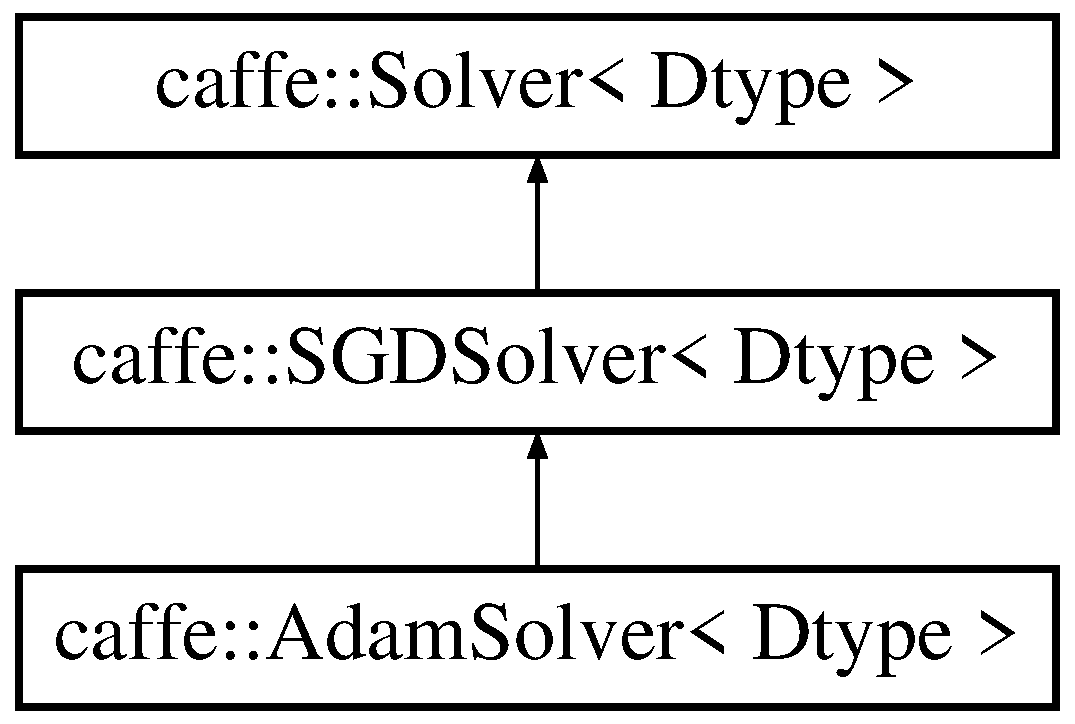
\includegraphics[height=3.000000cm]{classcaffe_1_1AdamSolver}
\end{center}
\end{figure}
\subsection*{Public Member Functions}
\begin{DoxyCompactItemize}
\item 
{\bfseries Adam\+Solver} (const Solver\+Parameter \&param)\hypertarget{classcaffe_1_1AdamSolver_a2591a6002658a955d8df6a2bf1a28f1e}{}\label{classcaffe_1_1AdamSolver_a2591a6002658a955d8df6a2bf1a28f1e}

\item 
{\bfseries Adam\+Solver} (const string \&param\+\_\+file)\hypertarget{classcaffe_1_1AdamSolver_adfd87b65ecd4c57591eefc24ac16e292}{}\label{classcaffe_1_1AdamSolver_adfd87b65ecd4c57591eefc24ac16e292}

\item 
virtual const char $\ast$ \hyperlink{classcaffe_1_1AdamSolver_af1909fb3b7eda6ce169d724a586dddd6}{type} () const \hypertarget{classcaffe_1_1AdamSolver_af1909fb3b7eda6ce169d724a586dddd6}{}\label{classcaffe_1_1AdamSolver_af1909fb3b7eda6ce169d724a586dddd6}

\begin{DoxyCompactList}\small\item\em Returns the solver type. \end{DoxyCompactList}\end{DoxyCompactItemize}
\subsection*{Protected Member Functions}
\begin{DoxyCompactItemize}
\item 
void {\bfseries Adam\+Pre\+Solve} ()\hypertarget{classcaffe_1_1AdamSolver_a72bbfc1fb2ec2194b183fa65f77ef1fb}{}\label{classcaffe_1_1AdamSolver_a72bbfc1fb2ec2194b183fa65f77ef1fb}

\item 
virtual void {\bfseries Compute\+Update\+Value} (int param\+\_\+id, Dtype rate)\hypertarget{classcaffe_1_1AdamSolver_a11f2c48ead67c91ba9e871acdbda1af8}{}\label{classcaffe_1_1AdamSolver_a11f2c48ead67c91ba9e871acdbda1af8}

\item 
{\bfseries D\+I\+S\+A\+B\+L\+E\+\_\+\+C\+O\+P\+Y\+\_\+\+A\+N\+D\+\_\+\+A\+S\+S\+I\+GN} (\hyperlink{classcaffe_1_1AdamSolver}{Adam\+Solver})\hypertarget{classcaffe_1_1AdamSolver_a5f192e195185ab841f083415333f5147}{}\label{classcaffe_1_1AdamSolver_a5f192e195185ab841f083415333f5147}

\end{DoxyCompactItemize}
\subsection*{Additional Inherited Members}


\subsection{Detailed Description}
\subsubsection*{template$<$typename Dtype$>$\\*
class caffe\+::\+Adam\+Solver$<$ Dtype $>$}

\hyperlink{classcaffe_1_1AdamSolver}{Adam\+Solver}, an algorithm for first-\/order gradient-\/based optimization of stochastic objective functions, based on adaptive estimates of lower-\/order moments. Described in \mbox{[}1\mbox{]}. 

\mbox{[}1\mbox{]} D. P. Kingma and J. L. Ba, \char`\"{}\+A\+D\+A\+M\+: A Method for Stochastic Optimization.\char`\"{} ar\+Xiv preprint ar\+Xiv\+:1412.\+6980v8 (2014). 

The documentation for this class was generated from the following files\+:\begin{DoxyCompactItemize}
\item 
include/caffe/sgd\+\_\+solvers.\+hpp\item 
src/caffe/solvers/adam\+\_\+solver.\+cpp\end{DoxyCompactItemize}

\hypertarget{classcaffe_1_1ArgMaxLayer}{}\section{caffe\+:\+:Arg\+Max\+Layer$<$ Dtype $>$ Class Template Reference}
\label{classcaffe_1_1ArgMaxLayer}\index{caffe\+::\+Arg\+Max\+Layer$<$ Dtype $>$@{caffe\+::\+Arg\+Max\+Layer$<$ Dtype $>$}}


Compute the index of the $ K $ max values for each datum across all dimensions $ (C \times H \times W) $.  




{\ttfamily \#include $<$argmax\+\_\+layer.\+hpp$>$}

Inheritance diagram for caffe\+:\+:Arg\+Max\+Layer$<$ Dtype $>$\+:\begin{figure}[H]
\begin{center}
\leavevmode
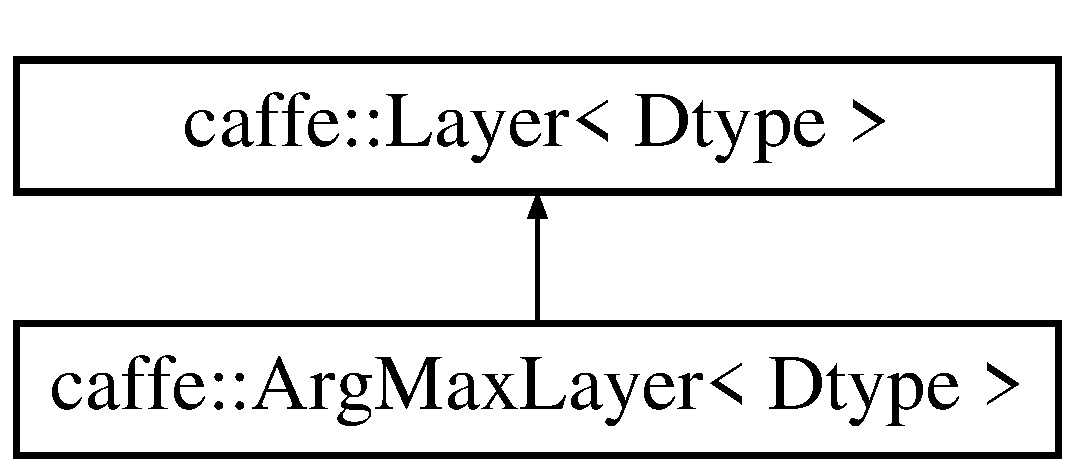
\includegraphics[height=2.000000cm]{classcaffe_1_1ArgMaxLayer}
\end{center}
\end{figure}
\subsection*{Public Member Functions}
\begin{DoxyCompactItemize}
\item 
\hyperlink{classcaffe_1_1ArgMaxLayer_a77429601f3d7f27b48720a1b703491be}{Arg\+Max\+Layer} (const Layer\+Parameter \&param)
\item 
virtual void \hyperlink{classcaffe_1_1ArgMaxLayer_a479814976e31716e670d63c126e5036f}{Layer\+Set\+Up} (const vector$<$ \hyperlink{classcaffe_1_1Blob}{Blob}$<$ Dtype $>$ $\ast$ $>$ \&bottom, const vector$<$ \hyperlink{classcaffe_1_1Blob}{Blob}$<$ Dtype $>$ $\ast$ $>$ \&top)
\begin{DoxyCompactList}\small\item\em Does layer-\/specific setup\+: your layer should implement this function as well as Reshape. \end{DoxyCompactList}\item 
virtual void \hyperlink{classcaffe_1_1ArgMaxLayer_ac379771528cba5db5ebafe318c412f05}{Reshape} (const vector$<$ \hyperlink{classcaffe_1_1Blob}{Blob}$<$ Dtype $>$ $\ast$ $>$ \&bottom, const vector$<$ \hyperlink{classcaffe_1_1Blob}{Blob}$<$ Dtype $>$ $\ast$ $>$ \&top)
\begin{DoxyCompactList}\small\item\em Adjust the shapes of top blobs and internal buffers to accommodate the shapes of the bottom blobs. \end{DoxyCompactList}\item 
virtual const char $\ast$ \hyperlink{classcaffe_1_1ArgMaxLayer_af54ed9ab47e4e82c53d86768d3cbb691}{type} () const \hypertarget{classcaffe_1_1ArgMaxLayer_af54ed9ab47e4e82c53d86768d3cbb691}{}\label{classcaffe_1_1ArgMaxLayer_af54ed9ab47e4e82c53d86768d3cbb691}

\begin{DoxyCompactList}\small\item\em Returns the layer type. \end{DoxyCompactList}\item 
virtual int \hyperlink{classcaffe_1_1ArgMaxLayer_ab9acebe420760d367c6e5808842411d0}{Exact\+Num\+Bottom\+Blobs} () const 
\begin{DoxyCompactList}\small\item\em Returns the exact number of bottom blobs required by the layer, or -\/1 if no exact number is required. \end{DoxyCompactList}\item 
virtual int \hyperlink{classcaffe_1_1ArgMaxLayer_acb86bae0a6dd2f01688ed4575830b874}{Exact\+Num\+Top\+Blobs} () const 
\begin{DoxyCompactList}\small\item\em Returns the exact number of top blobs required by the layer, or -\/1 if no exact number is required. \end{DoxyCompactList}\end{DoxyCompactItemize}
\subsection*{Protected Member Functions}
\begin{DoxyCompactItemize}
\item 
virtual void \hyperlink{classcaffe_1_1ArgMaxLayer_a6446de6fbb3f4310229b188b08fe2698}{Forward\+\_\+cpu} (const vector$<$ \hyperlink{classcaffe_1_1Blob}{Blob}$<$ Dtype $>$ $\ast$ $>$ \&bottom, const vector$<$ \hyperlink{classcaffe_1_1Blob}{Blob}$<$ Dtype $>$ $\ast$ $>$ \&top)
\item 
virtual void \hyperlink{classcaffe_1_1ArgMaxLayer_a31cab0f0ea73c0df25c347c0923ea9a0}{Backward\+\_\+cpu} (const vector$<$ \hyperlink{classcaffe_1_1Blob}{Blob}$<$ Dtype $>$ $\ast$ $>$ \&top, const vector$<$ bool $>$ \&propagate\+\_\+down, const vector$<$ \hyperlink{classcaffe_1_1Blob}{Blob}$<$ Dtype $>$ $\ast$ $>$ \&bottom)\hypertarget{classcaffe_1_1ArgMaxLayer_a31cab0f0ea73c0df25c347c0923ea9a0}{}\label{classcaffe_1_1ArgMaxLayer_a31cab0f0ea73c0df25c347c0923ea9a0}

\begin{DoxyCompactList}\small\item\em Not implemented (non-\/differentiable function) \end{DoxyCompactList}\end{DoxyCompactItemize}
\subsection*{Protected Attributes}
\begin{DoxyCompactItemize}
\item 
bool {\bfseries out\+\_\+max\+\_\+val\+\_\+}\hypertarget{classcaffe_1_1ArgMaxLayer_a80166873c75bdbb9a8aaa43e63543684}{}\label{classcaffe_1_1ArgMaxLayer_a80166873c75bdbb9a8aaa43e63543684}

\item 
size\+\_\+t {\bfseries top\+\_\+k\+\_\+}\hypertarget{classcaffe_1_1ArgMaxLayer_a936d87cd98fe0c508f5d7feb17c5f989}{}\label{classcaffe_1_1ArgMaxLayer_a936d87cd98fe0c508f5d7feb17c5f989}

\item 
bool {\bfseries has\+\_\+axis\+\_\+}\hypertarget{classcaffe_1_1ArgMaxLayer_aad30a415d4d23ce890f9ddf0c7efcb4b}{}\label{classcaffe_1_1ArgMaxLayer_aad30a415d4d23ce890f9ddf0c7efcb4b}

\item 
int {\bfseries axis\+\_\+}\hypertarget{classcaffe_1_1ArgMaxLayer_af0c7ee3334644eef4b7d7d47cb5890a7}{}\label{classcaffe_1_1ArgMaxLayer_af0c7ee3334644eef4b7d7d47cb5890a7}

\end{DoxyCompactItemize}


\subsection{Detailed Description}
\subsubsection*{template$<$typename Dtype$>$\\*
class caffe\+::\+Arg\+Max\+Layer$<$ Dtype $>$}

Compute the index of the $ K $ max values for each datum across all dimensions $ (C \times H \times W) $. 

Intended for use after a classification layer to produce a prediction. If parameter out\+\_\+max\+\_\+val is set to true, output is a vector of pairs (max\+\_\+ind, max\+\_\+val) for each image. The axis parameter specifies an axis along which to maximise.

N\+O\+TE\+: does not implement Backwards operation. 

\subsection{Constructor \& Destructor Documentation}
\index{caffe\+::\+Arg\+Max\+Layer@{caffe\+::\+Arg\+Max\+Layer}!Arg\+Max\+Layer@{Arg\+Max\+Layer}}
\index{Arg\+Max\+Layer@{Arg\+Max\+Layer}!caffe\+::\+Arg\+Max\+Layer@{caffe\+::\+Arg\+Max\+Layer}}
\subsubsection[{\texorpdfstring{Arg\+Max\+Layer(const Layer\+Parameter \&param)}{ArgMaxLayer(const LayerParameter &param)}}]{\setlength{\rightskip}{0pt plus 5cm}template$<$typename Dtype $>$ {\bf caffe\+::\+Arg\+Max\+Layer}$<$ Dtype $>$\+::{\bf Arg\+Max\+Layer} (
\begin{DoxyParamCaption}
\item[{const Layer\+Parameter \&}]{param}
\end{DoxyParamCaption}
)\hspace{0.3cm}{\ttfamily [inline]}, {\ttfamily [explicit]}}\hypertarget{classcaffe_1_1ArgMaxLayer_a77429601f3d7f27b48720a1b703491be}{}\label{classcaffe_1_1ArgMaxLayer_a77429601f3d7f27b48720a1b703491be}

\begin{DoxyParams}{Parameters}
{\em param} & provides Arg\+Max\+Parameter argmax\+\_\+param, with \hyperlink{classcaffe_1_1ArgMaxLayer}{Arg\+Max\+Layer} options\+:
\begin{DoxyItemize}
\item top\+\_\+k ({\bfseries optional} uint, default 1). the number $ K $ of maximal items to output.
\item out\+\_\+max\+\_\+val ({\bfseries optional} bool, default false). if set, output a vector of pairs (max\+\_\+ind, max\+\_\+val) unless axis is set then output max\+\_\+val along the specified axis.
\item axis ({\bfseries optional} int). if set, maximise along the specified axis else maximise the flattened trailing dimensions for each index of the first / num dimension. 
\end{DoxyItemize}\\
\hline
\end{DoxyParams}


\subsection{Member Function Documentation}
\index{caffe\+::\+Arg\+Max\+Layer@{caffe\+::\+Arg\+Max\+Layer}!Exact\+Num\+Bottom\+Blobs@{Exact\+Num\+Bottom\+Blobs}}
\index{Exact\+Num\+Bottom\+Blobs@{Exact\+Num\+Bottom\+Blobs}!caffe\+::\+Arg\+Max\+Layer@{caffe\+::\+Arg\+Max\+Layer}}
\subsubsection[{\texorpdfstring{Exact\+Num\+Bottom\+Blobs() const }{ExactNumBottomBlobs() const }}]{\setlength{\rightskip}{0pt plus 5cm}template$<$typename Dtype $>$ virtual int {\bf caffe\+::\+Arg\+Max\+Layer}$<$ Dtype $>$\+::Exact\+Num\+Bottom\+Blobs (
\begin{DoxyParamCaption}
{}
\end{DoxyParamCaption}
) const\hspace{0.3cm}{\ttfamily [inline]}, {\ttfamily [virtual]}}\hypertarget{classcaffe_1_1ArgMaxLayer_ab9acebe420760d367c6e5808842411d0}{}\label{classcaffe_1_1ArgMaxLayer_ab9acebe420760d367c6e5808842411d0}


Returns the exact number of bottom blobs required by the layer, or -\/1 if no exact number is required. 

This method should be overridden to return a non-\/negative value if your layer expects some exact number of bottom blobs. 

Reimplemented from \hyperlink{classcaffe_1_1Layer_a45c7a7943a8a6735ac433c9be11e0240}{caffe\+::\+Layer$<$ Dtype $>$}.

\index{caffe\+::\+Arg\+Max\+Layer@{caffe\+::\+Arg\+Max\+Layer}!Exact\+Num\+Top\+Blobs@{Exact\+Num\+Top\+Blobs}}
\index{Exact\+Num\+Top\+Blobs@{Exact\+Num\+Top\+Blobs}!caffe\+::\+Arg\+Max\+Layer@{caffe\+::\+Arg\+Max\+Layer}}
\subsubsection[{\texorpdfstring{Exact\+Num\+Top\+Blobs() const }{ExactNumTopBlobs() const }}]{\setlength{\rightskip}{0pt plus 5cm}template$<$typename Dtype $>$ virtual int {\bf caffe\+::\+Arg\+Max\+Layer}$<$ Dtype $>$\+::Exact\+Num\+Top\+Blobs (
\begin{DoxyParamCaption}
{}
\end{DoxyParamCaption}
) const\hspace{0.3cm}{\ttfamily [inline]}, {\ttfamily [virtual]}}\hypertarget{classcaffe_1_1ArgMaxLayer_acb86bae0a6dd2f01688ed4575830b874}{}\label{classcaffe_1_1ArgMaxLayer_acb86bae0a6dd2f01688ed4575830b874}


Returns the exact number of top blobs required by the layer, or -\/1 if no exact number is required. 

This method should be overridden to return a non-\/negative value if your layer expects some exact number of top blobs. 

Reimplemented from \hyperlink{classcaffe_1_1Layer_aa3c99ed707e8db683a3043412e151af8}{caffe\+::\+Layer$<$ Dtype $>$}.

\index{caffe\+::\+Arg\+Max\+Layer@{caffe\+::\+Arg\+Max\+Layer}!Forward\+\_\+cpu@{Forward\+\_\+cpu}}
\index{Forward\+\_\+cpu@{Forward\+\_\+cpu}!caffe\+::\+Arg\+Max\+Layer@{caffe\+::\+Arg\+Max\+Layer}}
\subsubsection[{\texorpdfstring{Forward\+\_\+cpu(const vector$<$ Blob$<$ Dtype $>$ $\ast$ $>$ \&bottom, const vector$<$ Blob$<$ Dtype $>$ $\ast$ $>$ \&top)}{Forward_cpu(const vector< Blob< Dtype > * > &bottom, const vector< Blob< Dtype > * > &top)}}]{\setlength{\rightskip}{0pt plus 5cm}template$<$typename Dtype $>$ void {\bf caffe\+::\+Arg\+Max\+Layer}$<$ Dtype $>$\+::Forward\+\_\+cpu (
\begin{DoxyParamCaption}
\item[{const vector$<$ {\bf Blob}$<$ Dtype $>$ $\ast$ $>$ \&}]{bottom, }
\item[{const vector$<$ {\bf Blob}$<$ Dtype $>$ $\ast$ $>$ \&}]{top}
\end{DoxyParamCaption}
)\hspace{0.3cm}{\ttfamily [protected]}, {\ttfamily [virtual]}}\hypertarget{classcaffe_1_1ArgMaxLayer_a6446de6fbb3f4310229b188b08fe2698}{}\label{classcaffe_1_1ArgMaxLayer_a6446de6fbb3f4310229b188b08fe2698}

\begin{DoxyParams}{Parameters}
{\em bottom} & input \hyperlink{classcaffe_1_1Blob}{Blob} vector (length 1)
\begin{DoxyEnumerate}
\item $ (N \times C \times H \times W) $ the inputs $ x $ 
\end{DoxyEnumerate}\\
\hline
{\em top} & output \hyperlink{classcaffe_1_1Blob}{Blob} vector (length 1)
\begin{DoxyEnumerate}
\item $ (N \times 1 \times K) $ or, if out\+\_\+max\+\_\+val $ (N \times 2 \times K) $ unless axis set than e.\+g. $ (N \times K \times H \times W) $ if axis == 1 the computed outputs $ y_n = \arg\max\limits_i x_{ni} $ (for $ K = 1 $). 
\end{DoxyEnumerate}\\
\hline
\end{DoxyParams}


Implements \hyperlink{classcaffe_1_1Layer_add965883f75bbf90c7a06f960cda7a1a}{caffe\+::\+Layer$<$ Dtype $>$}.

\index{caffe\+::\+Arg\+Max\+Layer@{caffe\+::\+Arg\+Max\+Layer}!Layer\+Set\+Up@{Layer\+Set\+Up}}
\index{Layer\+Set\+Up@{Layer\+Set\+Up}!caffe\+::\+Arg\+Max\+Layer@{caffe\+::\+Arg\+Max\+Layer}}
\subsubsection[{\texorpdfstring{Layer\+Set\+Up(const vector$<$ Blob$<$ Dtype $>$ $\ast$ $>$ \&bottom, const vector$<$ Blob$<$ Dtype $>$ $\ast$ $>$ \&top)}{LayerSetUp(const vector< Blob< Dtype > * > &bottom, const vector< Blob< Dtype > * > &top)}}]{\setlength{\rightskip}{0pt plus 5cm}template$<$typename Dtype $>$ void {\bf caffe\+::\+Arg\+Max\+Layer}$<$ Dtype $>$\+::Layer\+Set\+Up (
\begin{DoxyParamCaption}
\item[{const vector$<$ {\bf Blob}$<$ Dtype $>$ $\ast$ $>$ \&}]{bottom, }
\item[{const vector$<$ {\bf Blob}$<$ Dtype $>$ $\ast$ $>$ \&}]{top}
\end{DoxyParamCaption}
)\hspace{0.3cm}{\ttfamily [virtual]}}\hypertarget{classcaffe_1_1ArgMaxLayer_a479814976e31716e670d63c126e5036f}{}\label{classcaffe_1_1ArgMaxLayer_a479814976e31716e670d63c126e5036f}


Does layer-\/specific setup\+: your layer should implement this function as well as Reshape. 


\begin{DoxyParams}{Parameters}
{\em bottom} & the preshaped input blobs, whose data fields store the input data for this layer \\
\hline
{\em top} & the allocated but unshaped output blobs\\
\hline
\end{DoxyParams}
This method should do one-\/time layer specific setup. This includes reading and processing relevent parameters from the {\ttfamily layer\+\_\+param\+\_\+}. Setting up the shapes of top blobs and internal buffers should be done in {\ttfamily Reshape}, which will be called before the forward pass to adjust the top blob sizes. 

Reimplemented from \hyperlink{classcaffe_1_1Layer_a38dc2488bf319b8de5a7ac84e0045393}{caffe\+::\+Layer$<$ Dtype $>$}.

\index{caffe\+::\+Arg\+Max\+Layer@{caffe\+::\+Arg\+Max\+Layer}!Reshape@{Reshape}}
\index{Reshape@{Reshape}!caffe\+::\+Arg\+Max\+Layer@{caffe\+::\+Arg\+Max\+Layer}}
\subsubsection[{\texorpdfstring{Reshape(const vector$<$ Blob$<$ Dtype $>$ $\ast$ $>$ \&bottom, const vector$<$ Blob$<$ Dtype $>$ $\ast$ $>$ \&top)}{Reshape(const vector< Blob< Dtype > * > &bottom, const vector< Blob< Dtype > * > &top)}}]{\setlength{\rightskip}{0pt plus 5cm}template$<$typename Dtype $>$ void {\bf caffe\+::\+Arg\+Max\+Layer}$<$ Dtype $>$\+::Reshape (
\begin{DoxyParamCaption}
\item[{const vector$<$ {\bf Blob}$<$ Dtype $>$ $\ast$ $>$ \&}]{bottom, }
\item[{const vector$<$ {\bf Blob}$<$ Dtype $>$ $\ast$ $>$ \&}]{top}
\end{DoxyParamCaption}
)\hspace{0.3cm}{\ttfamily [virtual]}}\hypertarget{classcaffe_1_1ArgMaxLayer_ac379771528cba5db5ebafe318c412f05}{}\label{classcaffe_1_1ArgMaxLayer_ac379771528cba5db5ebafe318c412f05}


Adjust the shapes of top blobs and internal buffers to accommodate the shapes of the bottom blobs. 


\begin{DoxyParams}{Parameters}
{\em bottom} & the input blobs, with the requested input shapes \\
\hline
{\em top} & the top blobs, which should be reshaped as needed\\
\hline
\end{DoxyParams}
This method should reshape top blobs as needed according to the shapes of the bottom (input) blobs, as well as reshaping any internal buffers and making any other necessary adjustments so that the layer can accommodate the bottom blobs. 

Implements \hyperlink{classcaffe_1_1Layer_ad9d391b972c769c0ebee34ca6d1c973e}{caffe\+::\+Layer$<$ Dtype $>$}.



The documentation for this class was generated from the following files\+:\begin{DoxyCompactItemize}
\item 
include/caffe/layers/argmax\+\_\+layer.\+hpp\item 
src/caffe/layers/argmax\+\_\+layer.\+cpp\end{DoxyCompactItemize}

\hypertarget{classcaffe_1_1BaseConvolutionLayer}{}\section{caffe\+:\+:Base\+Convolution\+Layer$<$ Dtype $>$ Class Template Reference}
\label{classcaffe_1_1BaseConvolutionLayer}\index{caffe\+::\+Base\+Convolution\+Layer$<$ Dtype $>$@{caffe\+::\+Base\+Convolution\+Layer$<$ Dtype $>$}}


Abstract base class that factors out the B\+L\+AS code common to \hyperlink{classcaffe_1_1ConvolutionLayer}{Convolution\+Layer} and \hyperlink{classcaffe_1_1DeconvolutionLayer}{Deconvolution\+Layer}.  




{\ttfamily \#include $<$base\+\_\+conv\+\_\+layer.\+hpp$>$}

Inheritance diagram for caffe\+:\+:Base\+Convolution\+Layer$<$ Dtype $>$\+:\begin{figure}[H]
\begin{center}
\leavevmode
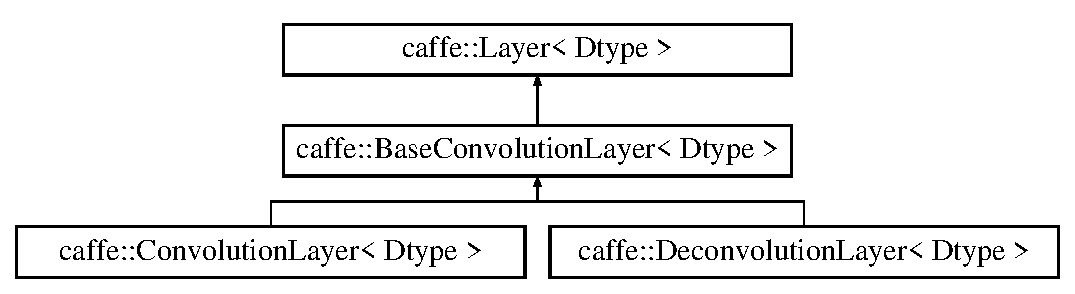
\includegraphics[height=3.000000cm]{classcaffe_1_1BaseConvolutionLayer}
\end{center}
\end{figure}
\subsection*{Public Member Functions}
\begin{DoxyCompactItemize}
\item 
{\bfseries Base\+Convolution\+Layer} (const Layer\+Parameter \&param)\hypertarget{classcaffe_1_1BaseConvolutionLayer_a42f9ea86a8ede098bda11f582a31ffc1}{}\label{classcaffe_1_1BaseConvolutionLayer_a42f9ea86a8ede098bda11f582a31ffc1}

\item 
virtual void \hyperlink{classcaffe_1_1BaseConvolutionLayer_a35c6389878e77ab0a4a479e5441563cc}{Layer\+Set\+Up} (const vector$<$ \hyperlink{classcaffe_1_1Blob}{Blob}$<$ Dtype $>$ $\ast$ $>$ \&bottom, const vector$<$ \hyperlink{classcaffe_1_1Blob}{Blob}$<$ Dtype $>$ $\ast$ $>$ \&top)
\begin{DoxyCompactList}\small\item\em Does layer-\/specific setup\+: your layer should implement this function as well as Reshape. \end{DoxyCompactList}\item 
virtual void \hyperlink{classcaffe_1_1BaseConvolutionLayer_ac330e2fb166bca496edd277b0495f6eb}{Reshape} (const vector$<$ \hyperlink{classcaffe_1_1Blob}{Blob}$<$ Dtype $>$ $\ast$ $>$ \&bottom, const vector$<$ \hyperlink{classcaffe_1_1Blob}{Blob}$<$ Dtype $>$ $\ast$ $>$ \&top)
\begin{DoxyCompactList}\small\item\em Adjust the shapes of top blobs and internal buffers to accommodate the shapes of the bottom blobs. \end{DoxyCompactList}\item 
virtual int \hyperlink{classcaffe_1_1BaseConvolutionLayer_a14a2760d3eafcfce766222f80e126fbe}{Min\+Bottom\+Blobs} () const 
\begin{DoxyCompactList}\small\item\em Returns the minimum number of bottom blobs required by the layer, or -\/1 if no minimum number is required. \end{DoxyCompactList}\item 
virtual int \hyperlink{classcaffe_1_1BaseConvolutionLayer_accd0683191124da91a3667acc57e5ecd}{Min\+Top\+Blobs} () const 
\begin{DoxyCompactList}\small\item\em Returns the minimum number of top blobs required by the layer, or -\/1 if no minimum number is required. \end{DoxyCompactList}\item 
virtual bool \hyperlink{classcaffe_1_1BaseConvolutionLayer_add4567680b9466cbae5804da6a76e2ee}{Equal\+Num\+Bottom\+Top\+Blobs} () const 
\begin{DoxyCompactList}\small\item\em Returns true if the layer requires an equal number of bottom and top blobs. \end{DoxyCompactList}\end{DoxyCompactItemize}
\subsection*{Protected Member Functions}
\begin{DoxyCompactItemize}
\item 
void {\bfseries forward\+\_\+cpu\+\_\+gemm} (const Dtype $\ast$input, const Dtype $\ast$weights, Dtype $\ast$output, bool skip\+\_\+im2col=false)\hypertarget{classcaffe_1_1BaseConvolutionLayer_a2870d22074426089e31afd864b989743}{}\label{classcaffe_1_1BaseConvolutionLayer_a2870d22074426089e31afd864b989743}

\item 
void {\bfseries forward\+\_\+cpu\+\_\+bias} (Dtype $\ast$output, const Dtype $\ast$bias)\hypertarget{classcaffe_1_1BaseConvolutionLayer_a00ede6bbe48c3a6dedd21308a48f979f}{}\label{classcaffe_1_1BaseConvolutionLayer_a00ede6bbe48c3a6dedd21308a48f979f}

\item 
void {\bfseries backward\+\_\+cpu\+\_\+gemm} (const Dtype $\ast$input, const Dtype $\ast$weights, Dtype $\ast$output)\hypertarget{classcaffe_1_1BaseConvolutionLayer_a3006035856c7f49371fe2b93ed38c935}{}\label{classcaffe_1_1BaseConvolutionLayer_a3006035856c7f49371fe2b93ed38c935}

\item 
void {\bfseries weight\+\_\+cpu\+\_\+gemm} (const Dtype $\ast$input, const Dtype $\ast$output, Dtype $\ast$weights)\hypertarget{classcaffe_1_1BaseConvolutionLayer_aa0ce44e831ad98176dc8c06f2069df2e}{}\label{classcaffe_1_1BaseConvolutionLayer_aa0ce44e831ad98176dc8c06f2069df2e}

\item 
void {\bfseries backward\+\_\+cpu\+\_\+bias} (Dtype $\ast$bias, const Dtype $\ast$input)\hypertarget{classcaffe_1_1BaseConvolutionLayer_a840ea8c0a485047a9760b7194b68db0c}{}\label{classcaffe_1_1BaseConvolutionLayer_a840ea8c0a485047a9760b7194b68db0c}

\item 
void {\bfseries forward\+\_\+gpu\+\_\+gemm} (const Dtype $\ast$col\+\_\+input, const Dtype $\ast$weights, Dtype $\ast$output, bool skip\+\_\+im2col=false)\hypertarget{classcaffe_1_1BaseConvolutionLayer_ace6f5e890e06e4812cf10e841f279346}{}\label{classcaffe_1_1BaseConvolutionLayer_ace6f5e890e06e4812cf10e841f279346}

\item 
void {\bfseries forward\+\_\+gpu\+\_\+bias} (Dtype $\ast$output, const Dtype $\ast$bias)\hypertarget{classcaffe_1_1BaseConvolutionLayer_a2a1f9d98d332411a481d82c10d76b474}{}\label{classcaffe_1_1BaseConvolutionLayer_a2a1f9d98d332411a481d82c10d76b474}

\item 
void {\bfseries backward\+\_\+gpu\+\_\+gemm} (const Dtype $\ast$input, const Dtype $\ast$weights, Dtype $\ast$col\+\_\+output)\hypertarget{classcaffe_1_1BaseConvolutionLayer_aece62d609b5fb36990ef6d5c48472efe}{}\label{classcaffe_1_1BaseConvolutionLayer_aece62d609b5fb36990ef6d5c48472efe}

\item 
void {\bfseries weight\+\_\+gpu\+\_\+gemm} (const Dtype $\ast$col\+\_\+input, const Dtype $\ast$output, Dtype $\ast$weights)\hypertarget{classcaffe_1_1BaseConvolutionLayer_a2c2e76ae5046570087f6af56180787b5}{}\label{classcaffe_1_1BaseConvolutionLayer_a2c2e76ae5046570087f6af56180787b5}

\item 
void {\bfseries backward\+\_\+gpu\+\_\+bias} (Dtype $\ast$bias, const Dtype $\ast$input)\hypertarget{classcaffe_1_1BaseConvolutionLayer_abbaf526a70e5106b79d8da94e8d4aa06}{}\label{classcaffe_1_1BaseConvolutionLayer_abbaf526a70e5106b79d8da94e8d4aa06}

\item 
int \hyperlink{classcaffe_1_1BaseConvolutionLayer_a6324d4ab918a7b09399aa85a8a03737d}{input\+\_\+shape} (int i)\hypertarget{classcaffe_1_1BaseConvolutionLayer_a6324d4ab918a7b09399aa85a8a03737d}{}\label{classcaffe_1_1BaseConvolutionLayer_a6324d4ab918a7b09399aa85a8a03737d}

\begin{DoxyCompactList}\small\item\em The spatial dimensions of the input. \end{DoxyCompactList}\item 
virtual bool {\bfseries reverse\+\_\+dimensions} ()=0\hypertarget{classcaffe_1_1BaseConvolutionLayer_affa7a2b5b583afc210f0c5dfe48842c8}{}\label{classcaffe_1_1BaseConvolutionLayer_affa7a2b5b583afc210f0c5dfe48842c8}

\item 
virtual void {\bfseries compute\+\_\+output\+\_\+shape} ()=0\hypertarget{classcaffe_1_1BaseConvolutionLayer_a552f16d43bf2470274102fe4fcde8759}{}\label{classcaffe_1_1BaseConvolutionLayer_a552f16d43bf2470274102fe4fcde8759}

\end{DoxyCompactItemize}
\subsection*{Protected Attributes}
\begin{DoxyCompactItemize}
\item 
\hyperlink{classcaffe_1_1Blob}{Blob}$<$ int $>$ \hyperlink{classcaffe_1_1BaseConvolutionLayer_a0a2f112eec8a7cbd13888185d4fb36b0}{kernel\+\_\+shape\+\_\+}\hypertarget{classcaffe_1_1BaseConvolutionLayer_a0a2f112eec8a7cbd13888185d4fb36b0}{}\label{classcaffe_1_1BaseConvolutionLayer_a0a2f112eec8a7cbd13888185d4fb36b0}

\begin{DoxyCompactList}\small\item\em The spatial dimensions of a filter kernel. \end{DoxyCompactList}\item 
\hyperlink{classcaffe_1_1Blob}{Blob}$<$ int $>$ \hyperlink{classcaffe_1_1BaseConvolutionLayer_af638d3d8e67c33443cb11cb000368e73}{stride\+\_\+}\hypertarget{classcaffe_1_1BaseConvolutionLayer_af638d3d8e67c33443cb11cb000368e73}{}\label{classcaffe_1_1BaseConvolutionLayer_af638d3d8e67c33443cb11cb000368e73}

\begin{DoxyCompactList}\small\item\em The spatial dimensions of the stride. \end{DoxyCompactList}\item 
\hyperlink{classcaffe_1_1Blob}{Blob}$<$ int $>$ \hyperlink{classcaffe_1_1BaseConvolutionLayer_a897ead2823e9031863e2151e71229e35}{pad\+\_\+}\hypertarget{classcaffe_1_1BaseConvolutionLayer_a897ead2823e9031863e2151e71229e35}{}\label{classcaffe_1_1BaseConvolutionLayer_a897ead2823e9031863e2151e71229e35}

\begin{DoxyCompactList}\small\item\em The spatial dimensions of the padding. \end{DoxyCompactList}\item 
\hyperlink{classcaffe_1_1Blob}{Blob}$<$ int $>$ \hyperlink{classcaffe_1_1BaseConvolutionLayer_a91f929109b5c05ba6086d4c2a741ad4a}{dilation\+\_\+}\hypertarget{classcaffe_1_1BaseConvolutionLayer_a91f929109b5c05ba6086d4c2a741ad4a}{}\label{classcaffe_1_1BaseConvolutionLayer_a91f929109b5c05ba6086d4c2a741ad4a}

\begin{DoxyCompactList}\small\item\em The spatial dimensions of the dilation. \end{DoxyCompactList}\item 
\hyperlink{classcaffe_1_1Blob}{Blob}$<$ int $>$ \hyperlink{classcaffe_1_1BaseConvolutionLayer_a63756d6ef00f6491939e539094c21397}{conv\+\_\+input\+\_\+shape\+\_\+}\hypertarget{classcaffe_1_1BaseConvolutionLayer_a63756d6ef00f6491939e539094c21397}{}\label{classcaffe_1_1BaseConvolutionLayer_a63756d6ef00f6491939e539094c21397}

\begin{DoxyCompactList}\small\item\em The spatial dimensions of the convolution input. \end{DoxyCompactList}\item 
vector$<$ int $>$ \hyperlink{classcaffe_1_1BaseConvolutionLayer_a9dd3f4ea6e17fe155efe537c120a3de4}{col\+\_\+buffer\+\_\+shape\+\_\+}\hypertarget{classcaffe_1_1BaseConvolutionLayer_a9dd3f4ea6e17fe155efe537c120a3de4}{}\label{classcaffe_1_1BaseConvolutionLayer_a9dd3f4ea6e17fe155efe537c120a3de4}

\begin{DoxyCompactList}\small\item\em The spatial dimensions of the col\+\_\+buffer. \end{DoxyCompactList}\item 
vector$<$ int $>$ \hyperlink{classcaffe_1_1BaseConvolutionLayer_af0892b61454ba086c4c74b78d910bf31}{output\+\_\+shape\+\_\+}\hypertarget{classcaffe_1_1BaseConvolutionLayer_af0892b61454ba086c4c74b78d910bf31}{}\label{classcaffe_1_1BaseConvolutionLayer_af0892b61454ba086c4c74b78d910bf31}

\begin{DoxyCompactList}\small\item\em The spatial dimensions of the output. \end{DoxyCompactList}\item 
const vector$<$ int $>$ $\ast$ {\bfseries bottom\+\_\+shape\+\_\+}\hypertarget{classcaffe_1_1BaseConvolutionLayer_a8a91469895adc7114eecee92bb4f81a1}{}\label{classcaffe_1_1BaseConvolutionLayer_a8a91469895adc7114eecee92bb4f81a1}

\item 
int {\bfseries num\+\_\+spatial\+\_\+axes\+\_\+}\hypertarget{classcaffe_1_1BaseConvolutionLayer_a8eac7ce95d86d01f026b649787a1920b}{}\label{classcaffe_1_1BaseConvolutionLayer_a8eac7ce95d86d01f026b649787a1920b}

\item 
int {\bfseries bottom\+\_\+dim\+\_\+}\hypertarget{classcaffe_1_1BaseConvolutionLayer_af5a73bde5834135df30eb2649bd510cb}{}\label{classcaffe_1_1BaseConvolutionLayer_af5a73bde5834135df30eb2649bd510cb}

\item 
int {\bfseries top\+\_\+dim\+\_\+}\hypertarget{classcaffe_1_1BaseConvolutionLayer_a2221107608862f0a81a97f87363967ec}{}\label{classcaffe_1_1BaseConvolutionLayer_a2221107608862f0a81a97f87363967ec}

\item 
int {\bfseries channel\+\_\+axis\+\_\+}\hypertarget{classcaffe_1_1BaseConvolutionLayer_a3f1ce7e7343b3c10a58913fc3728e6d2}{}\label{classcaffe_1_1BaseConvolutionLayer_a3f1ce7e7343b3c10a58913fc3728e6d2}

\item 
int {\bfseries num\+\_\+}\hypertarget{classcaffe_1_1BaseConvolutionLayer_a04e2625c95d319ff11bfb98ded1fe9e9}{}\label{classcaffe_1_1BaseConvolutionLayer_a04e2625c95d319ff11bfb98ded1fe9e9}

\item 
int {\bfseries channels\+\_\+}\hypertarget{classcaffe_1_1BaseConvolutionLayer_ab9f8d85682bd1bcded1bf4b87061f515}{}\label{classcaffe_1_1BaseConvolutionLayer_ab9f8d85682bd1bcded1bf4b87061f515}

\item 
int {\bfseries group\+\_\+}\hypertarget{classcaffe_1_1BaseConvolutionLayer_ae05b3ec701c6b0277ba5689b88d8fc24}{}\label{classcaffe_1_1BaseConvolutionLayer_ae05b3ec701c6b0277ba5689b88d8fc24}

\item 
int {\bfseries out\+\_\+spatial\+\_\+dim\+\_\+}\hypertarget{classcaffe_1_1BaseConvolutionLayer_a215df1c90a686e075c8851cb7561d289}{}\label{classcaffe_1_1BaseConvolutionLayer_a215df1c90a686e075c8851cb7561d289}

\item 
int {\bfseries weight\+\_\+offset\+\_\+}\hypertarget{classcaffe_1_1BaseConvolutionLayer_af7b74e11196840561a451813a5aa4321}{}\label{classcaffe_1_1BaseConvolutionLayer_af7b74e11196840561a451813a5aa4321}

\item 
int {\bfseries num\+\_\+output\+\_\+}\hypertarget{classcaffe_1_1BaseConvolutionLayer_ac22f72160f6b4ee54d1139095d09d853}{}\label{classcaffe_1_1BaseConvolutionLayer_ac22f72160f6b4ee54d1139095d09d853}

\item 
bool {\bfseries bias\+\_\+term\+\_\+}\hypertarget{classcaffe_1_1BaseConvolutionLayer_af984e3e89a7b9d6d930ed93d29e06cb4}{}\label{classcaffe_1_1BaseConvolutionLayer_af984e3e89a7b9d6d930ed93d29e06cb4}

\item 
bool {\bfseries is\+\_\+1x1\+\_\+}\hypertarget{classcaffe_1_1BaseConvolutionLayer_a4c0e8ca309c48e535713e9532c0475ff}{}\label{classcaffe_1_1BaseConvolutionLayer_a4c0e8ca309c48e535713e9532c0475ff}

\item 
bool {\bfseries force\+\_\+nd\+\_\+im2col\+\_\+}\hypertarget{classcaffe_1_1BaseConvolutionLayer_a4b572cb3c810f3beffaab4fb680c7823}{}\label{classcaffe_1_1BaseConvolutionLayer_a4b572cb3c810f3beffaab4fb680c7823}

\end{DoxyCompactItemize}


\subsection{Detailed Description}
\subsubsection*{template$<$typename Dtype$>$\\*
class caffe\+::\+Base\+Convolution\+Layer$<$ Dtype $>$}

Abstract base class that factors out the B\+L\+AS code common to \hyperlink{classcaffe_1_1ConvolutionLayer}{Convolution\+Layer} and \hyperlink{classcaffe_1_1DeconvolutionLayer}{Deconvolution\+Layer}. 

\subsection{Member Function Documentation}
\index{caffe\+::\+Base\+Convolution\+Layer@{caffe\+::\+Base\+Convolution\+Layer}!Equal\+Num\+Bottom\+Top\+Blobs@{Equal\+Num\+Bottom\+Top\+Blobs}}
\index{Equal\+Num\+Bottom\+Top\+Blobs@{Equal\+Num\+Bottom\+Top\+Blobs}!caffe\+::\+Base\+Convolution\+Layer@{caffe\+::\+Base\+Convolution\+Layer}}
\subsubsection[{\texorpdfstring{Equal\+Num\+Bottom\+Top\+Blobs() const }{EqualNumBottomTopBlobs() const }}]{\setlength{\rightskip}{0pt plus 5cm}template$<$typename Dtype $>$ virtual bool {\bf caffe\+::\+Base\+Convolution\+Layer}$<$ Dtype $>$\+::Equal\+Num\+Bottom\+Top\+Blobs (
\begin{DoxyParamCaption}
{}
\end{DoxyParamCaption}
) const\hspace{0.3cm}{\ttfamily [inline]}, {\ttfamily [virtual]}}\hypertarget{classcaffe_1_1BaseConvolutionLayer_add4567680b9466cbae5804da6a76e2ee}{}\label{classcaffe_1_1BaseConvolutionLayer_add4567680b9466cbae5804da6a76e2ee}


Returns true if the layer requires an equal number of bottom and top blobs. 

This method should be overridden to return true if your layer expects an equal number of bottom and top blobs. 

Reimplemented from \hyperlink{classcaffe_1_1Layer_ad412187a0483c310bd59fd5f957faf0d}{caffe\+::\+Layer$<$ Dtype $>$}.

\index{caffe\+::\+Base\+Convolution\+Layer@{caffe\+::\+Base\+Convolution\+Layer}!Layer\+Set\+Up@{Layer\+Set\+Up}}
\index{Layer\+Set\+Up@{Layer\+Set\+Up}!caffe\+::\+Base\+Convolution\+Layer@{caffe\+::\+Base\+Convolution\+Layer}}
\subsubsection[{\texorpdfstring{Layer\+Set\+Up(const vector$<$ Blob$<$ Dtype $>$ $\ast$ $>$ \&bottom, const vector$<$ Blob$<$ Dtype $>$ $\ast$ $>$ \&top)}{LayerSetUp(const vector< Blob< Dtype > * > &bottom, const vector< Blob< Dtype > * > &top)}}]{\setlength{\rightskip}{0pt plus 5cm}template$<$typename Dtype $>$ void {\bf caffe\+::\+Base\+Convolution\+Layer}$<$ Dtype $>$\+::Layer\+Set\+Up (
\begin{DoxyParamCaption}
\item[{const vector$<$ {\bf Blob}$<$ Dtype $>$ $\ast$ $>$ \&}]{bottom, }
\item[{const vector$<$ {\bf Blob}$<$ Dtype $>$ $\ast$ $>$ \&}]{top}
\end{DoxyParamCaption}
)\hspace{0.3cm}{\ttfamily [virtual]}}\hypertarget{classcaffe_1_1BaseConvolutionLayer_a35c6389878e77ab0a4a479e5441563cc}{}\label{classcaffe_1_1BaseConvolutionLayer_a35c6389878e77ab0a4a479e5441563cc}


Does layer-\/specific setup\+: your layer should implement this function as well as Reshape. 


\begin{DoxyParams}{Parameters}
{\em bottom} & the preshaped input blobs, whose data fields store the input data for this layer \\
\hline
{\em top} & the allocated but unshaped output blobs\\
\hline
\end{DoxyParams}
This method should do one-\/time layer specific setup. This includes reading and processing relevent parameters from the {\ttfamily layer\+\_\+param\+\_\+}. Setting up the shapes of top blobs and internal buffers should be done in {\ttfamily Reshape}, which will be called before the forward pass to adjust the top blob sizes. 

Reimplemented from \hyperlink{classcaffe_1_1Layer_a38dc2488bf319b8de5a7ac84e0045393}{caffe\+::\+Layer$<$ Dtype $>$}.

\index{caffe\+::\+Base\+Convolution\+Layer@{caffe\+::\+Base\+Convolution\+Layer}!Min\+Bottom\+Blobs@{Min\+Bottom\+Blobs}}
\index{Min\+Bottom\+Blobs@{Min\+Bottom\+Blobs}!caffe\+::\+Base\+Convolution\+Layer@{caffe\+::\+Base\+Convolution\+Layer}}
\subsubsection[{\texorpdfstring{Min\+Bottom\+Blobs() const }{MinBottomBlobs() const }}]{\setlength{\rightskip}{0pt plus 5cm}template$<$typename Dtype $>$ virtual int {\bf caffe\+::\+Base\+Convolution\+Layer}$<$ Dtype $>$\+::Min\+Bottom\+Blobs (
\begin{DoxyParamCaption}
{}
\end{DoxyParamCaption}
) const\hspace{0.3cm}{\ttfamily [inline]}, {\ttfamily [virtual]}}\hypertarget{classcaffe_1_1BaseConvolutionLayer_a14a2760d3eafcfce766222f80e126fbe}{}\label{classcaffe_1_1BaseConvolutionLayer_a14a2760d3eafcfce766222f80e126fbe}


Returns the minimum number of bottom blobs required by the layer, or -\/1 if no minimum number is required. 

This method should be overridden to return a non-\/negative value if your layer expects some minimum number of bottom blobs. 

Reimplemented from \hyperlink{classcaffe_1_1Layer_ade3eee97cc743c4e68fff7eba6484916}{caffe\+::\+Layer$<$ Dtype $>$}.

\index{caffe\+::\+Base\+Convolution\+Layer@{caffe\+::\+Base\+Convolution\+Layer}!Min\+Top\+Blobs@{Min\+Top\+Blobs}}
\index{Min\+Top\+Blobs@{Min\+Top\+Blobs}!caffe\+::\+Base\+Convolution\+Layer@{caffe\+::\+Base\+Convolution\+Layer}}
\subsubsection[{\texorpdfstring{Min\+Top\+Blobs() const }{MinTopBlobs() const }}]{\setlength{\rightskip}{0pt plus 5cm}template$<$typename Dtype $>$ virtual int {\bf caffe\+::\+Base\+Convolution\+Layer}$<$ Dtype $>$\+::Min\+Top\+Blobs (
\begin{DoxyParamCaption}
{}
\end{DoxyParamCaption}
) const\hspace{0.3cm}{\ttfamily [inline]}, {\ttfamily [virtual]}}\hypertarget{classcaffe_1_1BaseConvolutionLayer_accd0683191124da91a3667acc57e5ecd}{}\label{classcaffe_1_1BaseConvolutionLayer_accd0683191124da91a3667acc57e5ecd}


Returns the minimum number of top blobs required by the layer, or -\/1 if no minimum number is required. 

This method should be overridden to return a non-\/negative value if your layer expects some minimum number of top blobs. 

Reimplemented from \hyperlink{classcaffe_1_1Layer_a8bb143d58a740345fa2dc3d4204d553b}{caffe\+::\+Layer$<$ Dtype $>$}.

\index{caffe\+::\+Base\+Convolution\+Layer@{caffe\+::\+Base\+Convolution\+Layer}!Reshape@{Reshape}}
\index{Reshape@{Reshape}!caffe\+::\+Base\+Convolution\+Layer@{caffe\+::\+Base\+Convolution\+Layer}}
\subsubsection[{\texorpdfstring{Reshape(const vector$<$ Blob$<$ Dtype $>$ $\ast$ $>$ \&bottom, const vector$<$ Blob$<$ Dtype $>$ $\ast$ $>$ \&top)}{Reshape(const vector< Blob< Dtype > * > &bottom, const vector< Blob< Dtype > * > &top)}}]{\setlength{\rightskip}{0pt plus 5cm}template$<$typename Dtype $>$ void {\bf caffe\+::\+Base\+Convolution\+Layer}$<$ Dtype $>$\+::Reshape (
\begin{DoxyParamCaption}
\item[{const vector$<$ {\bf Blob}$<$ Dtype $>$ $\ast$ $>$ \&}]{bottom, }
\item[{const vector$<$ {\bf Blob}$<$ Dtype $>$ $\ast$ $>$ \&}]{top}
\end{DoxyParamCaption}
)\hspace{0.3cm}{\ttfamily [virtual]}}\hypertarget{classcaffe_1_1BaseConvolutionLayer_ac330e2fb166bca496edd277b0495f6eb}{}\label{classcaffe_1_1BaseConvolutionLayer_ac330e2fb166bca496edd277b0495f6eb}


Adjust the shapes of top blobs and internal buffers to accommodate the shapes of the bottom blobs. 


\begin{DoxyParams}{Parameters}
{\em bottom} & the input blobs, with the requested input shapes \\
\hline
{\em top} & the top blobs, which should be reshaped as needed\\
\hline
\end{DoxyParams}
This method should reshape top blobs as needed according to the shapes of the bottom (input) blobs, as well as reshaping any internal buffers and making any other necessary adjustments so that the layer can accommodate the bottom blobs. 

Implements \hyperlink{classcaffe_1_1Layer_ad9d391b972c769c0ebee34ca6d1c973e}{caffe\+::\+Layer$<$ Dtype $>$}.



The documentation for this class was generated from the following files\+:\begin{DoxyCompactItemize}
\item 
include/caffe/layers/base\+\_\+conv\+\_\+layer.\+hpp\item 
src/caffe/layers/base\+\_\+conv\+\_\+layer.\+cpp\end{DoxyCompactItemize}

\hypertarget{classcaffe_1_1BaseDataLayer}{}\section{caffe\+:\+:Base\+Data\+Layer$<$ Dtype $>$ Class Template Reference}
\label{classcaffe_1_1BaseDataLayer}\index{caffe\+::\+Base\+Data\+Layer$<$ Dtype $>$@{caffe\+::\+Base\+Data\+Layer$<$ Dtype $>$}}


Provides base for data layers that feed blobs to the \hyperlink{classcaffe_1_1Net}{Net}.  




{\ttfamily \#include $<$base\+\_\+data\+\_\+layer.\+hpp$>$}

Inheritance diagram for caffe\+:\+:Base\+Data\+Layer$<$ Dtype $>$\+:\begin{figure}[H]
\begin{center}
\leavevmode
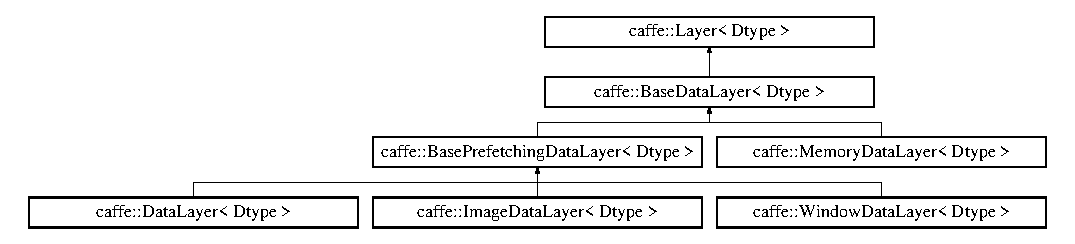
\includegraphics[height=2.828283cm]{classcaffe_1_1BaseDataLayer}
\end{center}
\end{figure}
\subsection*{Public Member Functions}
\begin{DoxyCompactItemize}
\item 
{\bfseries Base\+Data\+Layer} (const Layer\+Parameter \&param)\hypertarget{classcaffe_1_1BaseDataLayer_abf8b0153155bc04864ebeeb4c117d7a1}{}\label{classcaffe_1_1BaseDataLayer_abf8b0153155bc04864ebeeb4c117d7a1}

\item 
virtual void \hyperlink{classcaffe_1_1BaseDataLayer_a15f0c368230549ece6b91764704c9a73}{Layer\+Set\+Up} (const vector$<$ \hyperlink{classcaffe_1_1Blob}{Blob}$<$ Dtype $>$ $\ast$ $>$ \&bottom, const vector$<$ \hyperlink{classcaffe_1_1Blob}{Blob}$<$ Dtype $>$ $\ast$ $>$ \&top)
\begin{DoxyCompactList}\small\item\em Does layer-\/specific setup\+: your layer should implement this function as well as Reshape. \end{DoxyCompactList}\item 
virtual void {\bfseries Data\+Layer\+Set\+Up} (const vector$<$ \hyperlink{classcaffe_1_1Blob}{Blob}$<$ Dtype $>$ $\ast$ $>$ \&bottom, const vector$<$ \hyperlink{classcaffe_1_1Blob}{Blob}$<$ Dtype $>$ $\ast$ $>$ \&top)\hypertarget{classcaffe_1_1BaseDataLayer_a1c36ceb4162df320f1b9a41d289c8a8b}{}\label{classcaffe_1_1BaseDataLayer_a1c36ceb4162df320f1b9a41d289c8a8b}

\item 
virtual void \hyperlink{classcaffe_1_1BaseDataLayer_af2e62c1e0eee2b673973874c861df406}{Reshape} (const vector$<$ \hyperlink{classcaffe_1_1Blob}{Blob}$<$ Dtype $>$ $\ast$ $>$ \&bottom, const vector$<$ \hyperlink{classcaffe_1_1Blob}{Blob}$<$ Dtype $>$ $\ast$ $>$ \&top)
\begin{DoxyCompactList}\small\item\em Adjust the shapes of top blobs and internal buffers to accommodate the shapes of the bottom blobs. \end{DoxyCompactList}\item 
virtual void \hyperlink{classcaffe_1_1BaseDataLayer_ac0e1c8936407164b04aa98c11c36a22c}{Backward\+\_\+cpu} (const vector$<$ \hyperlink{classcaffe_1_1Blob}{Blob}$<$ Dtype $>$ $\ast$ $>$ \&top, const vector$<$ bool $>$ \&propagate\+\_\+down, const vector$<$ \hyperlink{classcaffe_1_1Blob}{Blob}$<$ Dtype $>$ $\ast$ $>$ \&bottom)\hypertarget{classcaffe_1_1BaseDataLayer_ac0e1c8936407164b04aa98c11c36a22c}{}\label{classcaffe_1_1BaseDataLayer_ac0e1c8936407164b04aa98c11c36a22c}

\begin{DoxyCompactList}\small\item\em Using the C\+PU device, compute the gradients for any parameters and for the bottom blobs if propagate\+\_\+down is true. \end{DoxyCompactList}\item 
virtual void \hyperlink{classcaffe_1_1BaseDataLayer_aa470016d58cfca4d75d1f3519e91d792}{Backward\+\_\+gpu} (const vector$<$ \hyperlink{classcaffe_1_1Blob}{Blob}$<$ Dtype $>$ $\ast$ $>$ \&top, const vector$<$ bool $>$ \&propagate\+\_\+down, const vector$<$ \hyperlink{classcaffe_1_1Blob}{Blob}$<$ Dtype $>$ $\ast$ $>$ \&bottom)\hypertarget{classcaffe_1_1BaseDataLayer_aa470016d58cfca4d75d1f3519e91d792}{}\label{classcaffe_1_1BaseDataLayer_aa470016d58cfca4d75d1f3519e91d792}

\begin{DoxyCompactList}\small\item\em Using the G\+PU device, compute the gradients for any parameters and for the bottom blobs if propagate\+\_\+down is true. Fall back to \hyperlink{classcaffe_1_1BaseDataLayer_ac0e1c8936407164b04aa98c11c36a22c}{Backward\+\_\+cpu()} if unavailable. \end{DoxyCompactList}\end{DoxyCompactItemize}
\subsection*{Protected Attributes}
\begin{DoxyCompactItemize}
\item 
Transformation\+Parameter {\bfseries transform\+\_\+param\+\_\+}\hypertarget{classcaffe_1_1BaseDataLayer_a325727e5c4f305a3ffa5c8efc211a1c9}{}\label{classcaffe_1_1BaseDataLayer_a325727e5c4f305a3ffa5c8efc211a1c9}

\item 
shared\+\_\+ptr$<$ \hyperlink{classcaffe_1_1DataTransformer}{Data\+Transformer}$<$ Dtype $>$ $>$ {\bfseries data\+\_\+transformer\+\_\+}\hypertarget{classcaffe_1_1BaseDataLayer_a8c0e6fd07b912dd62087024a5ddeaa00}{}\label{classcaffe_1_1BaseDataLayer_a8c0e6fd07b912dd62087024a5ddeaa00}

\item 
bool {\bfseries output\+\_\+labels\+\_\+}\hypertarget{classcaffe_1_1BaseDataLayer_a802076913164842d1f698014b489ca2e}{}\label{classcaffe_1_1BaseDataLayer_a802076913164842d1f698014b489ca2e}

\end{DoxyCompactItemize}
\subsection*{Additional Inherited Members}


\subsection{Detailed Description}
\subsubsection*{template$<$typename Dtype$>$\\*
class caffe\+::\+Base\+Data\+Layer$<$ Dtype $>$}

Provides base for data layers that feed blobs to the \hyperlink{classcaffe_1_1Net}{Net}. 

T\+O\+D\+O(dox)\+: thorough documentation for Forward and proto params. 

\subsection{Member Function Documentation}
\index{caffe\+::\+Base\+Data\+Layer@{caffe\+::\+Base\+Data\+Layer}!Layer\+Set\+Up@{Layer\+Set\+Up}}
\index{Layer\+Set\+Up@{Layer\+Set\+Up}!caffe\+::\+Base\+Data\+Layer@{caffe\+::\+Base\+Data\+Layer}}
\subsubsection[{\texorpdfstring{Layer\+Set\+Up(const vector$<$ Blob$<$ Dtype $>$ $\ast$ $>$ \&bottom, const vector$<$ Blob$<$ Dtype $>$ $\ast$ $>$ \&top)}{LayerSetUp(const vector< Blob< Dtype > * > &bottom, const vector< Blob< Dtype > * > &top)}}]{\setlength{\rightskip}{0pt plus 5cm}template$<$typename Dtype $>$ void {\bf caffe\+::\+Base\+Data\+Layer}$<$ Dtype $>$\+::Layer\+Set\+Up (
\begin{DoxyParamCaption}
\item[{const vector$<$ {\bf Blob}$<$ Dtype $>$ $\ast$ $>$ \&}]{bottom, }
\item[{const vector$<$ {\bf Blob}$<$ Dtype $>$ $\ast$ $>$ \&}]{top}
\end{DoxyParamCaption}
)\hspace{0.3cm}{\ttfamily [virtual]}}\hypertarget{classcaffe_1_1BaseDataLayer_a15f0c368230549ece6b91764704c9a73}{}\label{classcaffe_1_1BaseDataLayer_a15f0c368230549ece6b91764704c9a73}


Does layer-\/specific setup\+: your layer should implement this function as well as Reshape. 


\begin{DoxyParams}{Parameters}
{\em bottom} & the preshaped input blobs, whose data fields store the input data for this layer \\
\hline
{\em top} & the allocated but unshaped output blobs\\
\hline
\end{DoxyParams}
This method should do one-\/time layer specific setup. This includes reading and processing relevent parameters from the {\ttfamily layer\+\_\+param\+\_\+}. Setting up the shapes of top blobs and internal buffers should be done in {\ttfamily Reshape}, which will be called before the forward pass to adjust the top blob sizes. 

Reimplemented from \hyperlink{classcaffe_1_1Layer_a38dc2488bf319b8de5a7ac84e0045393}{caffe\+::\+Layer$<$ Dtype $>$}.



Reimplemented in \hyperlink{classcaffe_1_1BasePrefetchingDataLayer_af433228727bf4f3f3aaa85434efc93c5}{caffe\+::\+Base\+Prefetching\+Data\+Layer$<$ Dtype $>$}.

\index{caffe\+::\+Base\+Data\+Layer@{caffe\+::\+Base\+Data\+Layer}!Reshape@{Reshape}}
\index{Reshape@{Reshape}!caffe\+::\+Base\+Data\+Layer@{caffe\+::\+Base\+Data\+Layer}}
\subsubsection[{\texorpdfstring{Reshape(const vector$<$ Blob$<$ Dtype $>$ $\ast$ $>$ \&bottom, const vector$<$ Blob$<$ Dtype $>$ $\ast$ $>$ \&top)}{Reshape(const vector< Blob< Dtype > * > &bottom, const vector< Blob< Dtype > * > &top)}}]{\setlength{\rightskip}{0pt plus 5cm}template$<$typename Dtype $>$ virtual void {\bf caffe\+::\+Base\+Data\+Layer}$<$ Dtype $>$\+::Reshape (
\begin{DoxyParamCaption}
\item[{const vector$<$ {\bf Blob}$<$ Dtype $>$ $\ast$ $>$ \&}]{bottom, }
\item[{const vector$<$ {\bf Blob}$<$ Dtype $>$ $\ast$ $>$ \&}]{top}
\end{DoxyParamCaption}
)\hspace{0.3cm}{\ttfamily [inline]}, {\ttfamily [virtual]}}\hypertarget{classcaffe_1_1BaseDataLayer_af2e62c1e0eee2b673973874c861df406}{}\label{classcaffe_1_1BaseDataLayer_af2e62c1e0eee2b673973874c861df406}


Adjust the shapes of top blobs and internal buffers to accommodate the shapes of the bottom blobs. 


\begin{DoxyParams}{Parameters}
{\em bottom} & the input blobs, with the requested input shapes \\
\hline
{\em top} & the top blobs, which should be reshaped as needed\\
\hline
\end{DoxyParams}
This method should reshape top blobs as needed according to the shapes of the bottom (input) blobs, as well as reshaping any internal buffers and making any other necessary adjustments so that the layer can accommodate the bottom blobs. 

Implements \hyperlink{classcaffe_1_1Layer_ad9d391b972c769c0ebee34ca6d1c973e}{caffe\+::\+Layer$<$ Dtype $>$}.



The documentation for this class was generated from the following files\+:\begin{DoxyCompactItemize}
\item 
include/caffe/layers/base\+\_\+data\+\_\+layer.\+hpp\item 
src/caffe/layers/base\+\_\+data\+\_\+layer.\+cpp\end{DoxyCompactItemize}

\hypertarget{classcaffe_1_1BasePrefetchingDataLayer}{}\section{caffe\+:\+:Base\+Prefetching\+Data\+Layer$<$ Dtype $>$ Class Template Reference}
\label{classcaffe_1_1BasePrefetchingDataLayer}\index{caffe\+::\+Base\+Prefetching\+Data\+Layer$<$ Dtype $>$@{caffe\+::\+Base\+Prefetching\+Data\+Layer$<$ Dtype $>$}}
Inheritance diagram for caffe\+:\+:Base\+Prefetching\+Data\+Layer$<$ Dtype $>$\+:\begin{figure}[H]
\begin{center}
\leavevmode
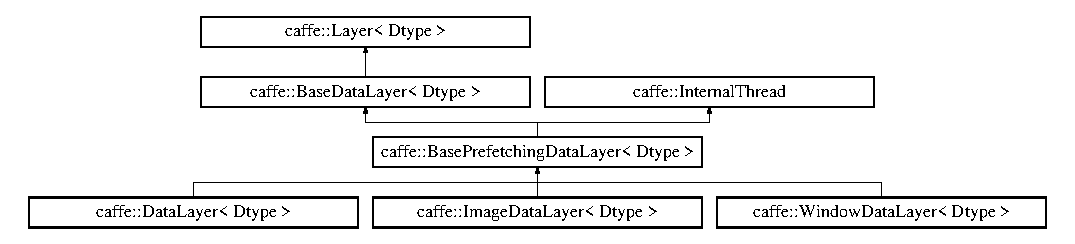
\includegraphics[height=2.828283cm]{classcaffe_1_1BasePrefetchingDataLayer}
\end{center}
\end{figure}
\subsection*{Public Member Functions}
\begin{DoxyCompactItemize}
\item 
{\bfseries Base\+Prefetching\+Data\+Layer} (const Layer\+Parameter \&param)\hypertarget{classcaffe_1_1BasePrefetchingDataLayer_a527e2b51c73759ea5f7e28ced6a371ef}{}\label{classcaffe_1_1BasePrefetchingDataLayer_a527e2b51c73759ea5f7e28ced6a371ef}

\item 
void \hyperlink{classcaffe_1_1BasePrefetchingDataLayer_af433228727bf4f3f3aaa85434efc93c5}{Layer\+Set\+Up} (const vector$<$ \hyperlink{classcaffe_1_1Blob}{Blob}$<$ Dtype $>$ $\ast$ $>$ \&bottom, const vector$<$ \hyperlink{classcaffe_1_1Blob}{Blob}$<$ Dtype $>$ $\ast$ $>$ \&top)
\begin{DoxyCompactList}\small\item\em Does layer-\/specific setup\+: your layer should implement this function as well as Reshape. \end{DoxyCompactList}\item 
virtual void \hyperlink{classcaffe_1_1BasePrefetchingDataLayer_a478965447079f7408d88c58f4a0dc49c}{Forward\+\_\+cpu} (const vector$<$ \hyperlink{classcaffe_1_1Blob}{Blob}$<$ Dtype $>$ $\ast$ $>$ \&bottom, const vector$<$ \hyperlink{classcaffe_1_1Blob}{Blob}$<$ Dtype $>$ $\ast$ $>$ \&top)\hypertarget{classcaffe_1_1BasePrefetchingDataLayer_a478965447079f7408d88c58f4a0dc49c}{}\label{classcaffe_1_1BasePrefetchingDataLayer_a478965447079f7408d88c58f4a0dc49c}

\begin{DoxyCompactList}\small\item\em Using the C\+PU device, compute the layer output. \end{DoxyCompactList}\item 
virtual void \hyperlink{classcaffe_1_1BasePrefetchingDataLayer_a950e9d525c7c07ef43567067805e7b70}{Forward\+\_\+gpu} (const vector$<$ \hyperlink{classcaffe_1_1Blob}{Blob}$<$ Dtype $>$ $\ast$ $>$ \&bottom, const vector$<$ \hyperlink{classcaffe_1_1Blob}{Blob}$<$ Dtype $>$ $\ast$ $>$ \&top)\hypertarget{classcaffe_1_1BasePrefetchingDataLayer_a950e9d525c7c07ef43567067805e7b70}{}\label{classcaffe_1_1BasePrefetchingDataLayer_a950e9d525c7c07ef43567067805e7b70}

\begin{DoxyCompactList}\small\item\em Using the G\+PU device, compute the layer output. Fall back to \hyperlink{classcaffe_1_1BasePrefetchingDataLayer_a478965447079f7408d88c58f4a0dc49c}{Forward\+\_\+cpu()} if unavailable. \end{DoxyCompactList}\end{DoxyCompactItemize}
\subsection*{Protected Member Functions}
\begin{DoxyCompactItemize}
\item 
virtual void {\bfseries Internal\+Thread\+Entry} ()\hypertarget{classcaffe_1_1BasePrefetchingDataLayer_aa2740717d51bd0b01646ace302991838}{}\label{classcaffe_1_1BasePrefetchingDataLayer_aa2740717d51bd0b01646ace302991838}

\item 
virtual void {\bfseries load\+\_\+batch} (\hyperlink{classcaffe_1_1Batch}{Batch}$<$ Dtype $>$ $\ast$batch)=0\hypertarget{classcaffe_1_1BasePrefetchingDataLayer_adab5b2e3013120a767d2be6ba609f045}{}\label{classcaffe_1_1BasePrefetchingDataLayer_adab5b2e3013120a767d2be6ba609f045}

\end{DoxyCompactItemize}
\subsection*{Protected Attributes}
\begin{DoxyCompactItemize}
\item 
vector$<$ shared\+\_\+ptr$<$ \hyperlink{classcaffe_1_1Batch}{Batch}$<$ Dtype $>$ $>$ $>$ {\bfseries prefetch\+\_\+}\hypertarget{classcaffe_1_1BasePrefetchingDataLayer_ae1beb4fe2338b694324e375624015a2c}{}\label{classcaffe_1_1BasePrefetchingDataLayer_ae1beb4fe2338b694324e375624015a2c}

\item 
\hyperlink{classcaffe_1_1BlockingQueue}{Blocking\+Queue}$<$ \hyperlink{classcaffe_1_1Batch}{Batch}$<$ Dtype $>$ $\ast$ $>$ {\bfseries prefetch\+\_\+free\+\_\+}\hypertarget{classcaffe_1_1BasePrefetchingDataLayer_a8ca3d78f628c0290ee7254a918f7e5db}{}\label{classcaffe_1_1BasePrefetchingDataLayer_a8ca3d78f628c0290ee7254a918f7e5db}

\item 
\hyperlink{classcaffe_1_1BlockingQueue}{Blocking\+Queue}$<$ \hyperlink{classcaffe_1_1Batch}{Batch}$<$ Dtype $>$ $\ast$ $>$ {\bfseries prefetch\+\_\+full\+\_\+}\hypertarget{classcaffe_1_1BasePrefetchingDataLayer_a93b1730c7e6b96c80488ad281bada2d4}{}\label{classcaffe_1_1BasePrefetchingDataLayer_a93b1730c7e6b96c80488ad281bada2d4}

\item 
\hyperlink{classcaffe_1_1Batch}{Batch}$<$ Dtype $>$ $\ast$ {\bfseries prefetch\+\_\+current\+\_\+}\hypertarget{classcaffe_1_1BasePrefetchingDataLayer_a4b95c4ad255203d052657695bc681a5c}{}\label{classcaffe_1_1BasePrefetchingDataLayer_a4b95c4ad255203d052657695bc681a5c}

\item 
\hyperlink{classcaffe_1_1Blob}{Blob}$<$ Dtype $>$ {\bfseries transformed\+\_\+data\+\_\+}\hypertarget{classcaffe_1_1BasePrefetchingDataLayer_afbff8f9e7c0e0f4007d2cc742b4ad874}{}\label{classcaffe_1_1BasePrefetchingDataLayer_afbff8f9e7c0e0f4007d2cc742b4ad874}

\end{DoxyCompactItemize}


\subsection{Member Function Documentation}
\index{caffe\+::\+Base\+Prefetching\+Data\+Layer@{caffe\+::\+Base\+Prefetching\+Data\+Layer}!Layer\+Set\+Up@{Layer\+Set\+Up}}
\index{Layer\+Set\+Up@{Layer\+Set\+Up}!caffe\+::\+Base\+Prefetching\+Data\+Layer@{caffe\+::\+Base\+Prefetching\+Data\+Layer}}
\subsubsection[{\texorpdfstring{Layer\+Set\+Up(const vector$<$ Blob$<$ Dtype $>$ $\ast$ $>$ \&bottom, const vector$<$ Blob$<$ Dtype $>$ $\ast$ $>$ \&top)}{LayerSetUp(const vector< Blob< Dtype > * > &bottom, const vector< Blob< Dtype > * > &top)}}]{\setlength{\rightskip}{0pt plus 5cm}template$<$typename Dtype $>$ void {\bf caffe\+::\+Base\+Prefetching\+Data\+Layer}$<$ Dtype $>$\+::Layer\+Set\+Up (
\begin{DoxyParamCaption}
\item[{const vector$<$ {\bf Blob}$<$ Dtype $>$ $\ast$ $>$ \&}]{bottom, }
\item[{const vector$<$ {\bf Blob}$<$ Dtype $>$ $\ast$ $>$ \&}]{top}
\end{DoxyParamCaption}
)\hspace{0.3cm}{\ttfamily [virtual]}}\hypertarget{classcaffe_1_1BasePrefetchingDataLayer_af433228727bf4f3f3aaa85434efc93c5}{}\label{classcaffe_1_1BasePrefetchingDataLayer_af433228727bf4f3f3aaa85434efc93c5}


Does layer-\/specific setup\+: your layer should implement this function as well as Reshape. 


\begin{DoxyParams}{Parameters}
{\em bottom} & the preshaped input blobs, whose data fields store the input data for this layer \\
\hline
{\em top} & the allocated but unshaped output blobs\\
\hline
\end{DoxyParams}
This method should do one-\/time layer specific setup. This includes reading and processing relevent parameters from the {\ttfamily layer\+\_\+param\+\_\+}. Setting up the shapes of top blobs and internal buffers should be done in {\ttfamily Reshape}, which will be called before the forward pass to adjust the top blob sizes. 

Reimplemented from \hyperlink{classcaffe_1_1BaseDataLayer_a15f0c368230549ece6b91764704c9a73}{caffe\+::\+Base\+Data\+Layer$<$ Dtype $>$}.



The documentation for this class was generated from the following files\+:\begin{DoxyCompactItemize}
\item 
include/caffe/layers/base\+\_\+data\+\_\+layer.\+hpp\item 
src/caffe/layers/base\+\_\+data\+\_\+layer.\+cpp\end{DoxyCompactItemize}

\hypertarget{classcaffe_1_1Batch}{}\section{caffe\+:\+:Batch$<$ Dtype $>$ Class Template Reference}
\label{classcaffe_1_1Batch}\index{caffe\+::\+Batch$<$ Dtype $>$@{caffe\+::\+Batch$<$ Dtype $>$}}
\subsection*{Public Attributes}
\begin{DoxyCompactItemize}
\item 
\hyperlink{classcaffe_1_1Blob}{Blob}$<$ Dtype $>$ {\bfseries data\+\_\+}\hypertarget{classcaffe_1_1Batch_aba928d78692d7bb97fe55578cee19c5b}{}\label{classcaffe_1_1Batch_aba928d78692d7bb97fe55578cee19c5b}

\item 
\hyperlink{classcaffe_1_1Blob}{Blob}$<$ Dtype $>$ {\bfseries label\+\_\+}\hypertarget{classcaffe_1_1Batch_ad9cb6471af708d5607521a81019f93a1}{}\label{classcaffe_1_1Batch_ad9cb6471af708d5607521a81019f93a1}

\end{DoxyCompactItemize}


The documentation for this class was generated from the following file\+:\begin{DoxyCompactItemize}
\item 
include/caffe/layers/base\+\_\+data\+\_\+layer.\+hpp\end{DoxyCompactItemize}

\hypertarget{classcaffe_1_1BatchNormLayer}{}\section{caffe\+:\+:Batch\+Norm\+Layer$<$ Dtype $>$ Class Template Reference}
\label{classcaffe_1_1BatchNormLayer}\index{caffe\+::\+Batch\+Norm\+Layer$<$ Dtype $>$@{caffe\+::\+Batch\+Norm\+Layer$<$ Dtype $>$}}


Normalizes the input to have 0-\/mean and/or unit (1) variance across the batch.  




{\ttfamily \#include $<$batch\+\_\+norm\+\_\+layer.\+hpp$>$}

Inheritance diagram for caffe\+:\+:Batch\+Norm\+Layer$<$ Dtype $>$\+:\begin{figure}[H]
\begin{center}
\leavevmode
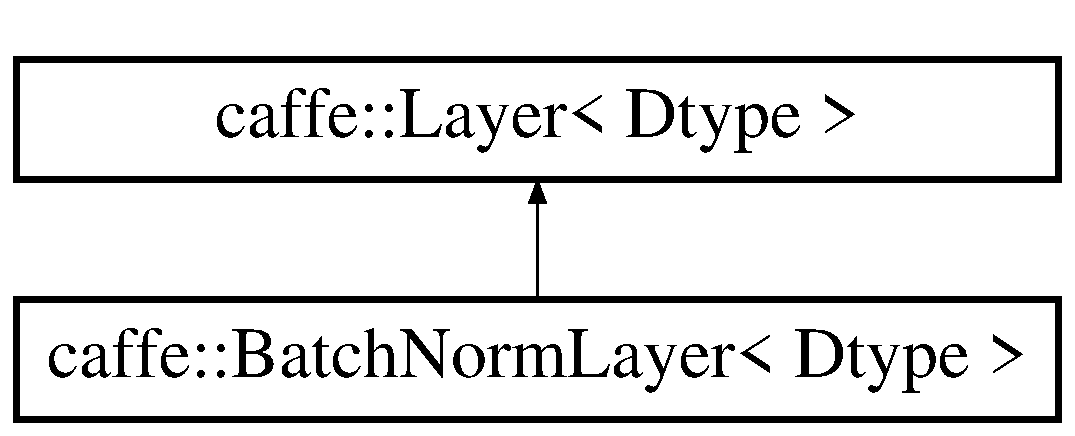
\includegraphics[height=2.000000cm]{classcaffe_1_1BatchNormLayer}
\end{center}
\end{figure}
\subsection*{Public Member Functions}
\begin{DoxyCompactItemize}
\item 
{\bfseries Batch\+Norm\+Layer} (const Layer\+Parameter \&param)\hypertarget{classcaffe_1_1BatchNormLayer_add0e20ed67cad3052669765cda52a7f0}{}\label{classcaffe_1_1BatchNormLayer_add0e20ed67cad3052669765cda52a7f0}

\item 
virtual void \hyperlink{classcaffe_1_1BatchNormLayer_ae4784dc3c124ea934b1d9736d465591f}{Layer\+Set\+Up} (const vector$<$ \hyperlink{classcaffe_1_1Blob}{Blob}$<$ Dtype $>$ $\ast$ $>$ \&bottom, const vector$<$ \hyperlink{classcaffe_1_1Blob}{Blob}$<$ Dtype $>$ $\ast$ $>$ \&top)
\begin{DoxyCompactList}\small\item\em Does layer-\/specific setup\+: your layer should implement this function as well as Reshape. \end{DoxyCompactList}\item 
virtual void \hyperlink{classcaffe_1_1BatchNormLayer_afb4c4da26887dfbd6d73ab35be17ed84}{Reshape} (const vector$<$ \hyperlink{classcaffe_1_1Blob}{Blob}$<$ Dtype $>$ $\ast$ $>$ \&bottom, const vector$<$ \hyperlink{classcaffe_1_1Blob}{Blob}$<$ Dtype $>$ $\ast$ $>$ \&top)
\begin{DoxyCompactList}\small\item\em Adjust the shapes of top blobs and internal buffers to accommodate the shapes of the bottom blobs. \end{DoxyCompactList}\item 
virtual const char $\ast$ \hyperlink{classcaffe_1_1BatchNormLayer_acf78346b46fa24e33337db9e155e4001}{type} () const \hypertarget{classcaffe_1_1BatchNormLayer_acf78346b46fa24e33337db9e155e4001}{}\label{classcaffe_1_1BatchNormLayer_acf78346b46fa24e33337db9e155e4001}

\begin{DoxyCompactList}\small\item\em Returns the layer type. \end{DoxyCompactList}\item 
virtual int \hyperlink{classcaffe_1_1BatchNormLayer_a30b42ad6c976170fc0a8c523682ff96a}{Exact\+Num\+Bottom\+Blobs} () const 
\begin{DoxyCompactList}\small\item\em Returns the exact number of bottom blobs required by the layer, or -\/1 if no exact number is required. \end{DoxyCompactList}\item 
virtual int \hyperlink{classcaffe_1_1BatchNormLayer_ad9fb4bf90a79a0a739ed1223628a88b9}{Exact\+Num\+Top\+Blobs} () const 
\begin{DoxyCompactList}\small\item\em Returns the exact number of top blobs required by the layer, or -\/1 if no exact number is required. \end{DoxyCompactList}\end{DoxyCompactItemize}
\subsection*{Protected Member Functions}
\begin{DoxyCompactItemize}
\item 
virtual void \hyperlink{classcaffe_1_1BatchNormLayer_a93fc10c42a94d9bf61fb10b73521b23b}{Forward\+\_\+cpu} (const vector$<$ \hyperlink{classcaffe_1_1Blob}{Blob}$<$ Dtype $>$ $\ast$ $>$ \&bottom, const vector$<$ \hyperlink{classcaffe_1_1Blob}{Blob}$<$ Dtype $>$ $\ast$ $>$ \&top)\hypertarget{classcaffe_1_1BatchNormLayer_a93fc10c42a94d9bf61fb10b73521b23b}{}\label{classcaffe_1_1BatchNormLayer_a93fc10c42a94d9bf61fb10b73521b23b}

\begin{DoxyCompactList}\small\item\em Using the C\+PU device, compute the layer output. \end{DoxyCompactList}\item 
virtual void \hyperlink{classcaffe_1_1BatchNormLayer_ae5832f8ba488345842129c99e743cfe6}{Forward\+\_\+gpu} (const vector$<$ \hyperlink{classcaffe_1_1Blob}{Blob}$<$ Dtype $>$ $\ast$ $>$ \&bottom, const vector$<$ \hyperlink{classcaffe_1_1Blob}{Blob}$<$ Dtype $>$ $\ast$ $>$ \&top)\hypertarget{classcaffe_1_1BatchNormLayer_ae5832f8ba488345842129c99e743cfe6}{}\label{classcaffe_1_1BatchNormLayer_ae5832f8ba488345842129c99e743cfe6}

\begin{DoxyCompactList}\small\item\em Using the G\+PU device, compute the layer output. Fall back to \hyperlink{classcaffe_1_1BatchNormLayer_a93fc10c42a94d9bf61fb10b73521b23b}{Forward\+\_\+cpu()} if unavailable. \end{DoxyCompactList}\item 
virtual void \hyperlink{classcaffe_1_1BatchNormLayer_ac3dd99d7fc010d3a2567034c50324b60}{Backward\+\_\+cpu} (const vector$<$ \hyperlink{classcaffe_1_1Blob}{Blob}$<$ Dtype $>$ $\ast$ $>$ \&top, const vector$<$ bool $>$ \&propagate\+\_\+down, const vector$<$ \hyperlink{classcaffe_1_1Blob}{Blob}$<$ Dtype $>$ $\ast$ $>$ \&bottom)\hypertarget{classcaffe_1_1BatchNormLayer_ac3dd99d7fc010d3a2567034c50324b60}{}\label{classcaffe_1_1BatchNormLayer_ac3dd99d7fc010d3a2567034c50324b60}

\begin{DoxyCompactList}\small\item\em Using the C\+PU device, compute the gradients for any parameters and for the bottom blobs if propagate\+\_\+down is true. \end{DoxyCompactList}\item 
virtual void \hyperlink{classcaffe_1_1BatchNormLayer_a4e3c00252a8f4b7891ca2b43f14bcdfb}{Backward\+\_\+gpu} (const vector$<$ \hyperlink{classcaffe_1_1Blob}{Blob}$<$ Dtype $>$ $\ast$ $>$ \&top, const vector$<$ bool $>$ \&propagate\+\_\+down, const vector$<$ \hyperlink{classcaffe_1_1Blob}{Blob}$<$ Dtype $>$ $\ast$ $>$ \&bottom)\hypertarget{classcaffe_1_1BatchNormLayer_a4e3c00252a8f4b7891ca2b43f14bcdfb}{}\label{classcaffe_1_1BatchNormLayer_a4e3c00252a8f4b7891ca2b43f14bcdfb}

\begin{DoxyCompactList}\small\item\em Using the G\+PU device, compute the gradients for any parameters and for the bottom blobs if propagate\+\_\+down is true. Fall back to \hyperlink{classcaffe_1_1BatchNormLayer_ac3dd99d7fc010d3a2567034c50324b60}{Backward\+\_\+cpu()} if unavailable. \end{DoxyCompactList}\end{DoxyCompactItemize}
\subsection*{Protected Attributes}
\begin{DoxyCompactItemize}
\item 
\hyperlink{classcaffe_1_1Blob}{Blob}$<$ Dtype $>$ {\bfseries mean\+\_\+}\hypertarget{classcaffe_1_1BatchNormLayer_a40bdb2eb1eb8c1af257d83d1ee34477e}{}\label{classcaffe_1_1BatchNormLayer_a40bdb2eb1eb8c1af257d83d1ee34477e}

\item 
\hyperlink{classcaffe_1_1Blob}{Blob}$<$ Dtype $>$ {\bfseries variance\+\_\+}\hypertarget{classcaffe_1_1BatchNormLayer_a60af867dc745b550056fdb0bf5253fb2}{}\label{classcaffe_1_1BatchNormLayer_a60af867dc745b550056fdb0bf5253fb2}

\item 
\hyperlink{classcaffe_1_1Blob}{Blob}$<$ Dtype $>$ {\bfseries temp\+\_\+}\hypertarget{classcaffe_1_1BatchNormLayer_a385f18e414274c8398d7f68f7a21fd47}{}\label{classcaffe_1_1BatchNormLayer_a385f18e414274c8398d7f68f7a21fd47}

\item 
\hyperlink{classcaffe_1_1Blob}{Blob}$<$ Dtype $>$ {\bfseries x\+\_\+norm\+\_\+}\hypertarget{classcaffe_1_1BatchNormLayer_ae6ff1b957b514a954dcb62ea5464d3eb}{}\label{classcaffe_1_1BatchNormLayer_ae6ff1b957b514a954dcb62ea5464d3eb}

\item 
bool {\bfseries use\+\_\+global\+\_\+stats\+\_\+}\hypertarget{classcaffe_1_1BatchNormLayer_ad3a29633c4b31c90bc8524f271279deb}{}\label{classcaffe_1_1BatchNormLayer_ad3a29633c4b31c90bc8524f271279deb}

\item 
Dtype {\bfseries moving\+\_\+average\+\_\+fraction\+\_\+}\hypertarget{classcaffe_1_1BatchNormLayer_a080385766fcb5df87d46e5ce9ed6168e}{}\label{classcaffe_1_1BatchNormLayer_a080385766fcb5df87d46e5ce9ed6168e}

\item 
int {\bfseries channels\+\_\+}\hypertarget{classcaffe_1_1BatchNormLayer_aceaba0d4877aefb36a320c9a147a613c}{}\label{classcaffe_1_1BatchNormLayer_aceaba0d4877aefb36a320c9a147a613c}

\item 
Dtype {\bfseries eps\+\_\+}\hypertarget{classcaffe_1_1BatchNormLayer_a578bf09a12d0ad6b6fb51600a1a1feb6}{}\label{classcaffe_1_1BatchNormLayer_a578bf09a12d0ad6b6fb51600a1a1feb6}

\item 
\hyperlink{classcaffe_1_1Blob}{Blob}$<$ Dtype $>$ {\bfseries batch\+\_\+sum\+\_\+multiplier\+\_\+}\hypertarget{classcaffe_1_1BatchNormLayer_a04b912c9e47737b4c91bf97bfd34c9ae}{}\label{classcaffe_1_1BatchNormLayer_a04b912c9e47737b4c91bf97bfd34c9ae}

\item 
\hyperlink{classcaffe_1_1Blob}{Blob}$<$ Dtype $>$ {\bfseries num\+\_\+by\+\_\+chans\+\_\+}\hypertarget{classcaffe_1_1BatchNormLayer_a18b26f0942f10d4de8562aca9c68e38d}{}\label{classcaffe_1_1BatchNormLayer_a18b26f0942f10d4de8562aca9c68e38d}

\item 
\hyperlink{classcaffe_1_1Blob}{Blob}$<$ Dtype $>$ {\bfseries spatial\+\_\+sum\+\_\+multiplier\+\_\+}\hypertarget{classcaffe_1_1BatchNormLayer_a1649265a7921b2fee4e99dd26069e74a}{}\label{classcaffe_1_1BatchNormLayer_a1649265a7921b2fee4e99dd26069e74a}

\end{DoxyCompactItemize}


\subsection{Detailed Description}
\subsubsection*{template$<$typename Dtype$>$\\*
class caffe\+::\+Batch\+Norm\+Layer$<$ Dtype $>$}

Normalizes the input to have 0-\/mean and/or unit (1) variance across the batch. 

This layer computes \hyperlink{classcaffe_1_1Batch}{Batch} Normalization as described in \mbox{[}1\mbox{]}. For each channel in the data (i.\+e. axis 1), it subtracts the mean and divides by the variance, where both statistics are computed across both spatial dimensions and across the different examples in the batch.

By default, during training time, the network is computing global mean/variance statistics via a running average, which is then used at test time to allow deterministic outputs for each input. You can manually toggle whether the network is accumulating or using the statistics via the use\+\_\+global\+\_\+stats option. For reference, these statistics are kept in the layer\textquotesingle{}s three blobs\+: (0) mean, (1) variance, and (2) moving average factor.

Note that the original paper also included a per-\/channel learned bias and scaling factor. To implement this in \hyperlink{classcaffe_1_1Caffe}{Caffe}, define a {\ttfamily \hyperlink{classcaffe_1_1ScaleLayer}{Scale\+Layer}} configured with {\ttfamily bias\+\_\+term\+: true} after each {\ttfamily \hyperlink{classcaffe_1_1BatchNormLayer}{Batch\+Norm\+Layer}} to handle both the bias and scaling factor.

\mbox{[}1\mbox{]} S. Ioffe and C. Szegedy, \char`\"{}\+Batch Normalization\+: Accelerating Deep Network
    Training by Reducing Internal Covariate Shift.\char`\"{} ar\+Xiv preprint ar\+Xiv\+:1502.\+03167 (2015).

T\+O\+D\+O(dox)\+: thorough documentation for Forward, Backward, and proto params. 

\subsection{Member Function Documentation}
\index{caffe\+::\+Batch\+Norm\+Layer@{caffe\+::\+Batch\+Norm\+Layer}!Exact\+Num\+Bottom\+Blobs@{Exact\+Num\+Bottom\+Blobs}}
\index{Exact\+Num\+Bottom\+Blobs@{Exact\+Num\+Bottom\+Blobs}!caffe\+::\+Batch\+Norm\+Layer@{caffe\+::\+Batch\+Norm\+Layer}}
\subsubsection[{\texorpdfstring{Exact\+Num\+Bottom\+Blobs() const }{ExactNumBottomBlobs() const }}]{\setlength{\rightskip}{0pt plus 5cm}template$<$typename Dtype $>$ virtual int {\bf caffe\+::\+Batch\+Norm\+Layer}$<$ Dtype $>$\+::Exact\+Num\+Bottom\+Blobs (
\begin{DoxyParamCaption}
{}
\end{DoxyParamCaption}
) const\hspace{0.3cm}{\ttfamily [inline]}, {\ttfamily [virtual]}}\hypertarget{classcaffe_1_1BatchNormLayer_a30b42ad6c976170fc0a8c523682ff96a}{}\label{classcaffe_1_1BatchNormLayer_a30b42ad6c976170fc0a8c523682ff96a}


Returns the exact number of bottom blobs required by the layer, or -\/1 if no exact number is required. 

This method should be overridden to return a non-\/negative value if your layer expects some exact number of bottom blobs. 

Reimplemented from \hyperlink{classcaffe_1_1Layer_a45c7a7943a8a6735ac433c9be11e0240}{caffe\+::\+Layer$<$ Dtype $>$}.

\index{caffe\+::\+Batch\+Norm\+Layer@{caffe\+::\+Batch\+Norm\+Layer}!Exact\+Num\+Top\+Blobs@{Exact\+Num\+Top\+Blobs}}
\index{Exact\+Num\+Top\+Blobs@{Exact\+Num\+Top\+Blobs}!caffe\+::\+Batch\+Norm\+Layer@{caffe\+::\+Batch\+Norm\+Layer}}
\subsubsection[{\texorpdfstring{Exact\+Num\+Top\+Blobs() const }{ExactNumTopBlobs() const }}]{\setlength{\rightskip}{0pt plus 5cm}template$<$typename Dtype $>$ virtual int {\bf caffe\+::\+Batch\+Norm\+Layer}$<$ Dtype $>$\+::Exact\+Num\+Top\+Blobs (
\begin{DoxyParamCaption}
{}
\end{DoxyParamCaption}
) const\hspace{0.3cm}{\ttfamily [inline]}, {\ttfamily [virtual]}}\hypertarget{classcaffe_1_1BatchNormLayer_ad9fb4bf90a79a0a739ed1223628a88b9}{}\label{classcaffe_1_1BatchNormLayer_ad9fb4bf90a79a0a739ed1223628a88b9}


Returns the exact number of top blobs required by the layer, or -\/1 if no exact number is required. 

This method should be overridden to return a non-\/negative value if your layer expects some exact number of top blobs. 

Reimplemented from \hyperlink{classcaffe_1_1Layer_aa3c99ed707e8db683a3043412e151af8}{caffe\+::\+Layer$<$ Dtype $>$}.

\index{caffe\+::\+Batch\+Norm\+Layer@{caffe\+::\+Batch\+Norm\+Layer}!Layer\+Set\+Up@{Layer\+Set\+Up}}
\index{Layer\+Set\+Up@{Layer\+Set\+Up}!caffe\+::\+Batch\+Norm\+Layer@{caffe\+::\+Batch\+Norm\+Layer}}
\subsubsection[{\texorpdfstring{Layer\+Set\+Up(const vector$<$ Blob$<$ Dtype $>$ $\ast$ $>$ \&bottom, const vector$<$ Blob$<$ Dtype $>$ $\ast$ $>$ \&top)}{LayerSetUp(const vector< Blob< Dtype > * > &bottom, const vector< Blob< Dtype > * > &top)}}]{\setlength{\rightskip}{0pt plus 5cm}template$<$typename Dtype $>$ void {\bf caffe\+::\+Batch\+Norm\+Layer}$<$ Dtype $>$\+::Layer\+Set\+Up (
\begin{DoxyParamCaption}
\item[{const vector$<$ {\bf Blob}$<$ Dtype $>$ $\ast$ $>$ \&}]{bottom, }
\item[{const vector$<$ {\bf Blob}$<$ Dtype $>$ $\ast$ $>$ \&}]{top}
\end{DoxyParamCaption}
)\hspace{0.3cm}{\ttfamily [virtual]}}\hypertarget{classcaffe_1_1BatchNormLayer_ae4784dc3c124ea934b1d9736d465591f}{}\label{classcaffe_1_1BatchNormLayer_ae4784dc3c124ea934b1d9736d465591f}


Does layer-\/specific setup\+: your layer should implement this function as well as Reshape. 


\begin{DoxyParams}{Parameters}
{\em bottom} & the preshaped input blobs, whose data fields store the input data for this layer \\
\hline
{\em top} & the allocated but unshaped output blobs\\
\hline
\end{DoxyParams}
This method should do one-\/time layer specific setup. This includes reading and processing relevent parameters from the {\ttfamily layer\+\_\+param\+\_\+}. Setting up the shapes of top blobs and internal buffers should be done in {\ttfamily Reshape}, which will be called before the forward pass to adjust the top blob sizes. 

Reimplemented from \hyperlink{classcaffe_1_1Layer_a38dc2488bf319b8de5a7ac84e0045393}{caffe\+::\+Layer$<$ Dtype $>$}.

\index{caffe\+::\+Batch\+Norm\+Layer@{caffe\+::\+Batch\+Norm\+Layer}!Reshape@{Reshape}}
\index{Reshape@{Reshape}!caffe\+::\+Batch\+Norm\+Layer@{caffe\+::\+Batch\+Norm\+Layer}}
\subsubsection[{\texorpdfstring{Reshape(const vector$<$ Blob$<$ Dtype $>$ $\ast$ $>$ \&bottom, const vector$<$ Blob$<$ Dtype $>$ $\ast$ $>$ \&top)}{Reshape(const vector< Blob< Dtype > * > &bottom, const vector< Blob< Dtype > * > &top)}}]{\setlength{\rightskip}{0pt plus 5cm}template$<$typename Dtype $>$ void {\bf caffe\+::\+Batch\+Norm\+Layer}$<$ Dtype $>$\+::Reshape (
\begin{DoxyParamCaption}
\item[{const vector$<$ {\bf Blob}$<$ Dtype $>$ $\ast$ $>$ \&}]{bottom, }
\item[{const vector$<$ {\bf Blob}$<$ Dtype $>$ $\ast$ $>$ \&}]{top}
\end{DoxyParamCaption}
)\hspace{0.3cm}{\ttfamily [virtual]}}\hypertarget{classcaffe_1_1BatchNormLayer_afb4c4da26887dfbd6d73ab35be17ed84}{}\label{classcaffe_1_1BatchNormLayer_afb4c4da26887dfbd6d73ab35be17ed84}


Adjust the shapes of top blobs and internal buffers to accommodate the shapes of the bottom blobs. 


\begin{DoxyParams}{Parameters}
{\em bottom} & the input blobs, with the requested input shapes \\
\hline
{\em top} & the top blobs, which should be reshaped as needed\\
\hline
\end{DoxyParams}
This method should reshape top blobs as needed according to the shapes of the bottom (input) blobs, as well as reshaping any internal buffers and making any other necessary adjustments so that the layer can accommodate the bottom blobs. 

Implements \hyperlink{classcaffe_1_1Layer_ad9d391b972c769c0ebee34ca6d1c973e}{caffe\+::\+Layer$<$ Dtype $>$}.



The documentation for this class was generated from the following files\+:\begin{DoxyCompactItemize}
\item 
include/caffe/layers/batch\+\_\+norm\+\_\+layer.\+hpp\item 
src/caffe/layers/batch\+\_\+norm\+\_\+layer.\+cpp\end{DoxyCompactItemize}

\hypertarget{classcaffe_1_1BatchReindexLayer}{}\section{caffe\+:\+:Batch\+Reindex\+Layer$<$ Dtype $>$ Class Template Reference}
\label{classcaffe_1_1BatchReindexLayer}\index{caffe\+::\+Batch\+Reindex\+Layer$<$ Dtype $>$@{caffe\+::\+Batch\+Reindex\+Layer$<$ Dtype $>$}}


Index into the input blob along its first axis.  




{\ttfamily \#include $<$batch\+\_\+reindex\+\_\+layer.\+hpp$>$}

Inheritance diagram for caffe\+:\+:Batch\+Reindex\+Layer$<$ Dtype $>$\+:\begin{figure}[H]
\begin{center}
\leavevmode
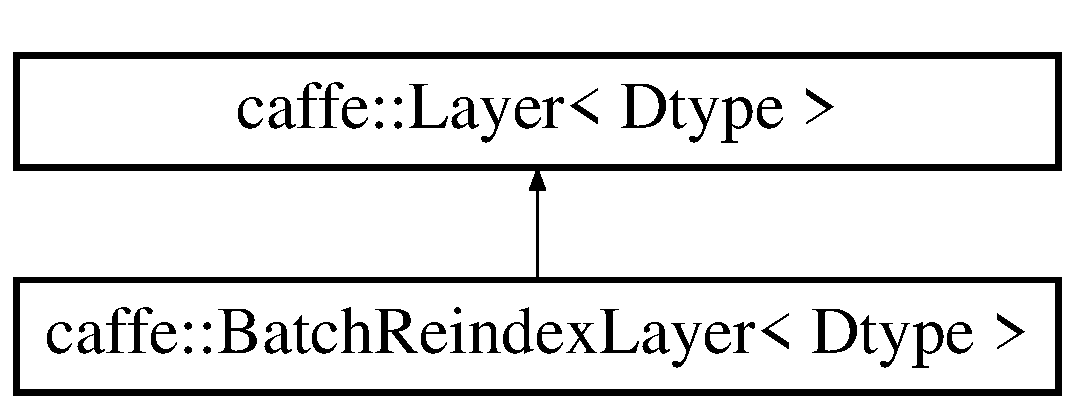
\includegraphics[height=2.000000cm]{classcaffe_1_1BatchReindexLayer}
\end{center}
\end{figure}
\subsection*{Public Member Functions}
\begin{DoxyCompactItemize}
\item 
{\bfseries Batch\+Reindex\+Layer} (const Layer\+Parameter \&param)\hypertarget{classcaffe_1_1BatchReindexLayer_a5585d02e701ad89b5ef46ec9340af7b6}{}\label{classcaffe_1_1BatchReindexLayer_a5585d02e701ad89b5ef46ec9340af7b6}

\item 
virtual void \hyperlink{classcaffe_1_1BatchReindexLayer_a4e39964037e5a0b168892b8128a2fef3}{Reshape} (const vector$<$ \hyperlink{classcaffe_1_1Blob}{Blob}$<$ Dtype $>$ $\ast$ $>$ \&bottom, const vector$<$ \hyperlink{classcaffe_1_1Blob}{Blob}$<$ Dtype $>$ $\ast$ $>$ \&top)
\begin{DoxyCompactList}\small\item\em Adjust the shapes of top blobs and internal buffers to accommodate the shapes of the bottom blobs. \end{DoxyCompactList}\item 
virtual const char $\ast$ \hyperlink{classcaffe_1_1BatchReindexLayer_abc303548e6724a91f942b42394b390f2}{type} () const \hypertarget{classcaffe_1_1BatchReindexLayer_abc303548e6724a91f942b42394b390f2}{}\label{classcaffe_1_1BatchReindexLayer_abc303548e6724a91f942b42394b390f2}

\begin{DoxyCompactList}\small\item\em Returns the layer type. \end{DoxyCompactList}\item 
virtual int \hyperlink{classcaffe_1_1BatchReindexLayer_ab84d37975127bfe16593c082731c6f55}{Exact\+Num\+Bottom\+Blobs} () const 
\begin{DoxyCompactList}\small\item\em Returns the exact number of bottom blobs required by the layer, or -\/1 if no exact number is required. \end{DoxyCompactList}\item 
virtual int \hyperlink{classcaffe_1_1BatchReindexLayer_afc9d0ae372b83e2b9e82228893313dc3}{Exact\+Num\+Top\+Blobs} () const 
\begin{DoxyCompactList}\small\item\em Returns the exact number of top blobs required by the layer, or -\/1 if no exact number is required. \end{DoxyCompactList}\end{DoxyCompactItemize}
\subsection*{Protected Member Functions}
\begin{DoxyCompactItemize}
\item 
virtual void \hyperlink{classcaffe_1_1BatchReindexLayer_acd40a7447f50cfa797422b457cdb739f}{Forward\+\_\+cpu} (const vector$<$ \hyperlink{classcaffe_1_1Blob}{Blob}$<$ Dtype $>$ $\ast$ $>$ \&bottom, const vector$<$ \hyperlink{classcaffe_1_1Blob}{Blob}$<$ Dtype $>$ $\ast$ $>$ \&top)
\item 
virtual void \hyperlink{classcaffe_1_1BatchReindexLayer_ac542edcc5400f3cd18b44c25ee36f784}{Forward\+\_\+gpu} (const vector$<$ \hyperlink{classcaffe_1_1Blob}{Blob}$<$ Dtype $>$ $\ast$ $>$ \&bottom, const vector$<$ \hyperlink{classcaffe_1_1Blob}{Blob}$<$ Dtype $>$ $\ast$ $>$ \&top)\hypertarget{classcaffe_1_1BatchReindexLayer_ac542edcc5400f3cd18b44c25ee36f784}{}\label{classcaffe_1_1BatchReindexLayer_ac542edcc5400f3cd18b44c25ee36f784}

\begin{DoxyCompactList}\small\item\em Using the G\+PU device, compute the layer output. Fall back to \hyperlink{classcaffe_1_1BatchReindexLayer_acd40a7447f50cfa797422b457cdb739f}{Forward\+\_\+cpu()} if unavailable. \end{DoxyCompactList}\item 
virtual void \hyperlink{classcaffe_1_1BatchReindexLayer_a6b50b080097dabed56d0cb333b07ebea}{Backward\+\_\+cpu} (const vector$<$ \hyperlink{classcaffe_1_1Blob}{Blob}$<$ Dtype $>$ $\ast$ $>$ \&top, const vector$<$ bool $>$ \&propagate\+\_\+down, const vector$<$ \hyperlink{classcaffe_1_1Blob}{Blob}$<$ Dtype $>$ $\ast$ $>$ \&bottom)
\begin{DoxyCompactList}\small\item\em Computes the error gradient w.\+r.\+t. the reordered input. \end{DoxyCompactList}\item 
virtual void \hyperlink{classcaffe_1_1BatchReindexLayer_a785a6eed33119deab1edcd3b90265318}{Backward\+\_\+gpu} (const vector$<$ \hyperlink{classcaffe_1_1Blob}{Blob}$<$ Dtype $>$ $\ast$ $>$ \&top, const vector$<$ bool $>$ \&propagate\+\_\+down, const vector$<$ \hyperlink{classcaffe_1_1Blob}{Blob}$<$ Dtype $>$ $\ast$ $>$ \&bottom)\hypertarget{classcaffe_1_1BatchReindexLayer_a785a6eed33119deab1edcd3b90265318}{}\label{classcaffe_1_1BatchReindexLayer_a785a6eed33119deab1edcd3b90265318}

\begin{DoxyCompactList}\small\item\em Using the G\+PU device, compute the gradients for any parameters and for the bottom blobs if propagate\+\_\+down is true. Fall back to \hyperlink{classcaffe_1_1BatchReindexLayer_a6b50b080097dabed56d0cb333b07ebea}{Backward\+\_\+cpu()} if unavailable. \end{DoxyCompactList}\end{DoxyCompactItemize}
\subsection*{Additional Inherited Members}


\subsection{Detailed Description}
\subsubsection*{template$<$typename Dtype$>$\\*
class caffe\+::\+Batch\+Reindex\+Layer$<$ Dtype $>$}

Index into the input blob along its first axis. 

This layer can be used to select, reorder, and even replicate examples in a batch. The second blob is cast to int and treated as an index into the first axis of the first blob. 

\subsection{Member Function Documentation}
\index{caffe\+::\+Batch\+Reindex\+Layer@{caffe\+::\+Batch\+Reindex\+Layer}!Backward\+\_\+cpu@{Backward\+\_\+cpu}}
\index{Backward\+\_\+cpu@{Backward\+\_\+cpu}!caffe\+::\+Batch\+Reindex\+Layer@{caffe\+::\+Batch\+Reindex\+Layer}}
\subsubsection[{\texorpdfstring{Backward\+\_\+cpu(const vector$<$ Blob$<$ Dtype $>$ $\ast$ $>$ \&top, const vector$<$ bool $>$ \&propagate\+\_\+down, const vector$<$ Blob$<$ Dtype $>$ $\ast$ $>$ \&bottom)}{Backward_cpu(const vector< Blob< Dtype > * > &top, const vector< bool > &propagate_down, const vector< Blob< Dtype > * > &bottom)}}]{\setlength{\rightskip}{0pt plus 5cm}template$<$typename Dtype $>$ void {\bf caffe\+::\+Batch\+Reindex\+Layer}$<$ Dtype $>$\+::Backward\+\_\+cpu (
\begin{DoxyParamCaption}
\item[{const vector$<$ {\bf Blob}$<$ Dtype $>$ $\ast$ $>$ \&}]{top, }
\item[{const vector$<$ bool $>$ \&}]{propagate\+\_\+down, }
\item[{const vector$<$ {\bf Blob}$<$ Dtype $>$ $\ast$ $>$ \&}]{bottom}
\end{DoxyParamCaption}
)\hspace{0.3cm}{\ttfamily [protected]}, {\ttfamily [virtual]}}\hypertarget{classcaffe_1_1BatchReindexLayer_a6b50b080097dabed56d0cb333b07ebea}{}\label{classcaffe_1_1BatchReindexLayer_a6b50b080097dabed56d0cb333b07ebea}


Computes the error gradient w.\+r.\+t. the reordered input. 


\begin{DoxyParams}{Parameters}
{\em top} & output \hyperlink{classcaffe_1_1Blob}{Blob} vector (length 1), providing the error gradient with respect to the outputs
\begin{DoxyEnumerate}
\item $ (M \times ...) $\+: containing error gradients $ \frac{\partial E}{\partial y} $ with respect to concatenated outputs $ y $ 
\end{DoxyEnumerate}\\
\hline
{\em propagate\+\_\+down} & see \hyperlink{classcaffe_1_1Layer_a53df1e081767e07bfb4c81657f4acd0a}{Layer\+::\+Backward}. \\
\hline
{\em bottom} & input \hyperlink{classcaffe_1_1Blob}{Blob} vector (length 2)\+:
\begin{DoxyItemize}
\item $ \frac{\partial E}{\partial y} $ is de-\/indexed (summing where required) back to the input x\+\_\+1
\item This layer cannot backprop to x\+\_\+2, i.\+e. propagate\+\_\+down\mbox{[}1\mbox{]} must be false. 
\end{DoxyItemize}\\
\hline
\end{DoxyParams}


Implements \hyperlink{classcaffe_1_1Layer_a64d15855f882af4b82e83fa993c4e7c6}{caffe\+::\+Layer$<$ Dtype $>$}.

\index{caffe\+::\+Batch\+Reindex\+Layer@{caffe\+::\+Batch\+Reindex\+Layer}!Exact\+Num\+Bottom\+Blobs@{Exact\+Num\+Bottom\+Blobs}}
\index{Exact\+Num\+Bottom\+Blobs@{Exact\+Num\+Bottom\+Blobs}!caffe\+::\+Batch\+Reindex\+Layer@{caffe\+::\+Batch\+Reindex\+Layer}}
\subsubsection[{\texorpdfstring{Exact\+Num\+Bottom\+Blobs() const }{ExactNumBottomBlobs() const }}]{\setlength{\rightskip}{0pt plus 5cm}template$<$typename Dtype $>$ virtual int {\bf caffe\+::\+Batch\+Reindex\+Layer}$<$ Dtype $>$\+::Exact\+Num\+Bottom\+Blobs (
\begin{DoxyParamCaption}
{}
\end{DoxyParamCaption}
) const\hspace{0.3cm}{\ttfamily [inline]}, {\ttfamily [virtual]}}\hypertarget{classcaffe_1_1BatchReindexLayer_ab84d37975127bfe16593c082731c6f55}{}\label{classcaffe_1_1BatchReindexLayer_ab84d37975127bfe16593c082731c6f55}


Returns the exact number of bottom blobs required by the layer, or -\/1 if no exact number is required. 

This method should be overridden to return a non-\/negative value if your layer expects some exact number of bottom blobs. 

Reimplemented from \hyperlink{classcaffe_1_1Layer_a45c7a7943a8a6735ac433c9be11e0240}{caffe\+::\+Layer$<$ Dtype $>$}.

\index{caffe\+::\+Batch\+Reindex\+Layer@{caffe\+::\+Batch\+Reindex\+Layer}!Exact\+Num\+Top\+Blobs@{Exact\+Num\+Top\+Blobs}}
\index{Exact\+Num\+Top\+Blobs@{Exact\+Num\+Top\+Blobs}!caffe\+::\+Batch\+Reindex\+Layer@{caffe\+::\+Batch\+Reindex\+Layer}}
\subsubsection[{\texorpdfstring{Exact\+Num\+Top\+Blobs() const }{ExactNumTopBlobs() const }}]{\setlength{\rightskip}{0pt plus 5cm}template$<$typename Dtype $>$ virtual int {\bf caffe\+::\+Batch\+Reindex\+Layer}$<$ Dtype $>$\+::Exact\+Num\+Top\+Blobs (
\begin{DoxyParamCaption}
{}
\end{DoxyParamCaption}
) const\hspace{0.3cm}{\ttfamily [inline]}, {\ttfamily [virtual]}}\hypertarget{classcaffe_1_1BatchReindexLayer_afc9d0ae372b83e2b9e82228893313dc3}{}\label{classcaffe_1_1BatchReindexLayer_afc9d0ae372b83e2b9e82228893313dc3}


Returns the exact number of top blobs required by the layer, or -\/1 if no exact number is required. 

This method should be overridden to return a non-\/negative value if your layer expects some exact number of top blobs. 

Reimplemented from \hyperlink{classcaffe_1_1Layer_aa3c99ed707e8db683a3043412e151af8}{caffe\+::\+Layer$<$ Dtype $>$}.

\index{caffe\+::\+Batch\+Reindex\+Layer@{caffe\+::\+Batch\+Reindex\+Layer}!Forward\+\_\+cpu@{Forward\+\_\+cpu}}
\index{Forward\+\_\+cpu@{Forward\+\_\+cpu}!caffe\+::\+Batch\+Reindex\+Layer@{caffe\+::\+Batch\+Reindex\+Layer}}
\subsubsection[{\texorpdfstring{Forward\+\_\+cpu(const vector$<$ Blob$<$ Dtype $>$ $\ast$ $>$ \&bottom, const vector$<$ Blob$<$ Dtype $>$ $\ast$ $>$ \&top)}{Forward_cpu(const vector< Blob< Dtype > * > &bottom, const vector< Blob< Dtype > * > &top)}}]{\setlength{\rightskip}{0pt plus 5cm}template$<$typename Dtype $>$ void {\bf caffe\+::\+Batch\+Reindex\+Layer}$<$ Dtype $>$\+::Forward\+\_\+cpu (
\begin{DoxyParamCaption}
\item[{const vector$<$ {\bf Blob}$<$ Dtype $>$ $\ast$ $>$ \&}]{bottom, }
\item[{const vector$<$ {\bf Blob}$<$ Dtype $>$ $\ast$ $>$ \&}]{top}
\end{DoxyParamCaption}
)\hspace{0.3cm}{\ttfamily [protected]}, {\ttfamily [virtual]}}\hypertarget{classcaffe_1_1BatchReindexLayer_acd40a7447f50cfa797422b457cdb739f}{}\label{classcaffe_1_1BatchReindexLayer_acd40a7447f50cfa797422b457cdb739f}

\begin{DoxyParams}{Parameters}
{\em bottom} & input \hyperlink{classcaffe_1_1Blob}{Blob} vector (length 2+)
\begin{DoxyEnumerate}
\item $ (N \times ...) $ the inputs $ x_1 $
\item $ (M) $ the inputs $ x_2 $ 
\end{DoxyEnumerate}\\
\hline
{\em top} & output \hyperlink{classcaffe_1_1Blob}{Blob} vector (length 1)
\begin{DoxyEnumerate}
\item $ (M \times ...) $\+: the reindexed array $ y = x_1[x_2] $ 
\end{DoxyEnumerate}\\
\hline
\end{DoxyParams}


Implements \hyperlink{classcaffe_1_1Layer_add965883f75bbf90c7a06f960cda7a1a}{caffe\+::\+Layer$<$ Dtype $>$}.

\index{caffe\+::\+Batch\+Reindex\+Layer@{caffe\+::\+Batch\+Reindex\+Layer}!Reshape@{Reshape}}
\index{Reshape@{Reshape}!caffe\+::\+Batch\+Reindex\+Layer@{caffe\+::\+Batch\+Reindex\+Layer}}
\subsubsection[{\texorpdfstring{Reshape(const vector$<$ Blob$<$ Dtype $>$ $\ast$ $>$ \&bottom, const vector$<$ Blob$<$ Dtype $>$ $\ast$ $>$ \&top)}{Reshape(const vector< Blob< Dtype > * > &bottom, const vector< Blob< Dtype > * > &top)}}]{\setlength{\rightskip}{0pt plus 5cm}template$<$typename Dtype $>$ void {\bf caffe\+::\+Batch\+Reindex\+Layer}$<$ Dtype $>$\+::Reshape (
\begin{DoxyParamCaption}
\item[{const vector$<$ {\bf Blob}$<$ Dtype $>$ $\ast$ $>$ \&}]{bottom, }
\item[{const vector$<$ {\bf Blob}$<$ Dtype $>$ $\ast$ $>$ \&}]{top}
\end{DoxyParamCaption}
)\hspace{0.3cm}{\ttfamily [virtual]}}\hypertarget{classcaffe_1_1BatchReindexLayer_a4e39964037e5a0b168892b8128a2fef3}{}\label{classcaffe_1_1BatchReindexLayer_a4e39964037e5a0b168892b8128a2fef3}


Adjust the shapes of top blobs and internal buffers to accommodate the shapes of the bottom blobs. 


\begin{DoxyParams}{Parameters}
{\em bottom} & the input blobs, with the requested input shapes \\
\hline
{\em top} & the top blobs, which should be reshaped as needed\\
\hline
\end{DoxyParams}
This method should reshape top blobs as needed according to the shapes of the bottom (input) blobs, as well as reshaping any internal buffers and making any other necessary adjustments so that the layer can accommodate the bottom blobs. 

Implements \hyperlink{classcaffe_1_1Layer_ad9d391b972c769c0ebee34ca6d1c973e}{caffe\+::\+Layer$<$ Dtype $>$}.



The documentation for this class was generated from the following files\+:\begin{DoxyCompactItemize}
\item 
include/caffe/layers/batch\+\_\+reindex\+\_\+layer.\+hpp\item 
src/caffe/layers/batch\+\_\+reindex\+\_\+layer.\+cpp\end{DoxyCompactItemize}

\hypertarget{classcaffe_1_1BiasLayer}{}\section{caffe\+:\+:Bias\+Layer$<$ Dtype $>$ Class Template Reference}
\label{classcaffe_1_1BiasLayer}\index{caffe\+::\+Bias\+Layer$<$ Dtype $>$@{caffe\+::\+Bias\+Layer$<$ Dtype $>$}}


Computes a sum of two input Blobs, with the shape of the latter \hyperlink{classcaffe_1_1Blob}{Blob} \char`\"{}broadcast\char`\"{} to match the shape of the former. Equivalent to tiling the latter \hyperlink{classcaffe_1_1Blob}{Blob}, then computing the elementwise sum.  




{\ttfamily \#include $<$bias\+\_\+layer.\+hpp$>$}

Inheritance diagram for caffe\+:\+:Bias\+Layer$<$ Dtype $>$\+:\begin{figure}[H]
\begin{center}
\leavevmode
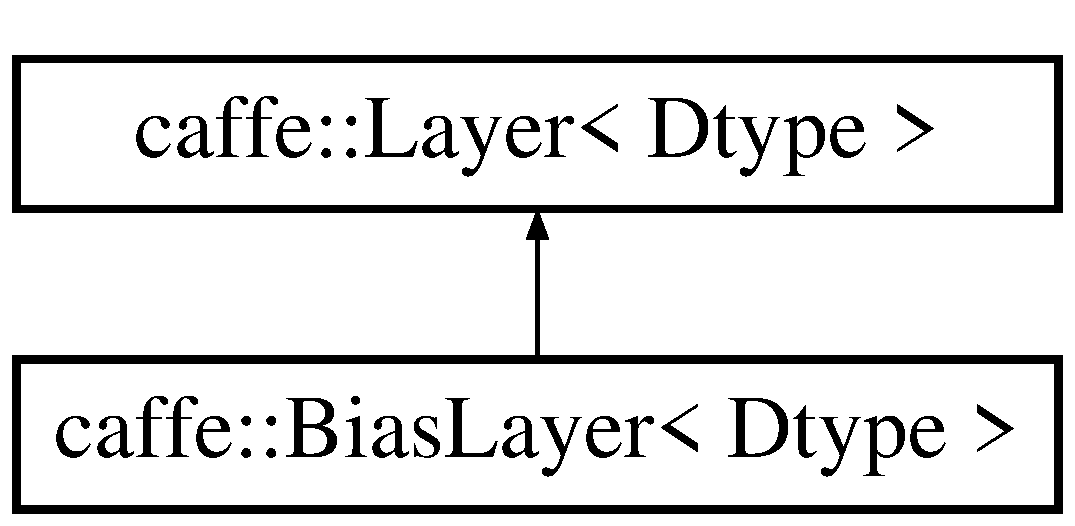
\includegraphics[height=2.000000cm]{classcaffe_1_1BiasLayer}
\end{center}
\end{figure}
\subsection*{Public Member Functions}
\begin{DoxyCompactItemize}
\item 
{\bfseries Bias\+Layer} (const Layer\+Parameter \&param)\hypertarget{classcaffe_1_1BiasLayer_a12e9da7fe06423dd2aaa0d1aba1ae460}{}\label{classcaffe_1_1BiasLayer_a12e9da7fe06423dd2aaa0d1aba1ae460}

\item 
virtual void \hyperlink{classcaffe_1_1BiasLayer_a88b3f3aad8ec2640c16a0c7bfdbf116a}{Layer\+Set\+Up} (const vector$<$ \hyperlink{classcaffe_1_1Blob}{Blob}$<$ Dtype $>$ $\ast$ $>$ \&bottom, const vector$<$ \hyperlink{classcaffe_1_1Blob}{Blob}$<$ Dtype $>$ $\ast$ $>$ \&top)
\begin{DoxyCompactList}\small\item\em Does layer-\/specific setup\+: your layer should implement this function as well as Reshape. \end{DoxyCompactList}\item 
virtual void \hyperlink{classcaffe_1_1BiasLayer_a6062d64c98cb115c304c78fe424091c3}{Reshape} (const vector$<$ \hyperlink{classcaffe_1_1Blob}{Blob}$<$ Dtype $>$ $\ast$ $>$ \&bottom, const vector$<$ \hyperlink{classcaffe_1_1Blob}{Blob}$<$ Dtype $>$ $\ast$ $>$ \&top)
\begin{DoxyCompactList}\small\item\em Adjust the shapes of top blobs and internal buffers to accommodate the shapes of the bottom blobs. \end{DoxyCompactList}\item 
virtual const char $\ast$ \hyperlink{classcaffe_1_1BiasLayer_aaa97578fe0968c367848dbc41c64e215}{type} () const \hypertarget{classcaffe_1_1BiasLayer_aaa97578fe0968c367848dbc41c64e215}{}\label{classcaffe_1_1BiasLayer_aaa97578fe0968c367848dbc41c64e215}

\begin{DoxyCompactList}\small\item\em Returns the layer type. \end{DoxyCompactList}\item 
virtual int \hyperlink{classcaffe_1_1BiasLayer_aafd8821a1dd5a649ece00c1f0b41ff1a}{Min\+Bottom\+Blobs} () const 
\begin{DoxyCompactList}\small\item\em Returns the minimum number of bottom blobs required by the layer, or -\/1 if no minimum number is required. \end{DoxyCompactList}\item 
virtual int \hyperlink{classcaffe_1_1BiasLayer_ac8c6e5a34a6a4ca1585e41ce6f01dab5}{Max\+Bottom\+Blobs} () const 
\begin{DoxyCompactList}\small\item\em Returns the maximum number of bottom blobs required by the layer, or -\/1 if no maximum number is required. \end{DoxyCompactList}\item 
virtual int \hyperlink{classcaffe_1_1BiasLayer_a62bf10551992b95ecd499f1ce50f9465}{Exact\+Num\+Top\+Blobs} () const 
\begin{DoxyCompactList}\small\item\em Returns the exact number of top blobs required by the layer, or -\/1 if no exact number is required. \end{DoxyCompactList}\item 
virtual void \hyperlink{classcaffe_1_1BiasLayer_a168a9381f352e88e62ca7dd12f1bdfb3}{Forward\+\_\+cpu} (const vector$<$ \hyperlink{classcaffe_1_1Blob}{Blob}$<$ Dtype $>$ $\ast$ $>$ \&bottom, const vector$<$ \hyperlink{classcaffe_1_1Blob}{Blob}$<$ Dtype $>$ $\ast$ $>$ \&top)\hypertarget{classcaffe_1_1BiasLayer_a168a9381f352e88e62ca7dd12f1bdfb3}{}\label{classcaffe_1_1BiasLayer_a168a9381f352e88e62ca7dd12f1bdfb3}

\begin{DoxyCompactList}\small\item\em Using the C\+PU device, compute the layer output. \end{DoxyCompactList}\item 
virtual void \hyperlink{classcaffe_1_1BiasLayer_a4040f9ddceaac10f0e90b3e73cc6403c}{Forward\+\_\+gpu} (const vector$<$ \hyperlink{classcaffe_1_1Blob}{Blob}$<$ Dtype $>$ $\ast$ $>$ \&bottom, const vector$<$ \hyperlink{classcaffe_1_1Blob}{Blob}$<$ Dtype $>$ $\ast$ $>$ \&top)\hypertarget{classcaffe_1_1BiasLayer_a4040f9ddceaac10f0e90b3e73cc6403c}{}\label{classcaffe_1_1BiasLayer_a4040f9ddceaac10f0e90b3e73cc6403c}

\begin{DoxyCompactList}\small\item\em Using the G\+PU device, compute the layer output. Fall back to \hyperlink{classcaffe_1_1BiasLayer_a168a9381f352e88e62ca7dd12f1bdfb3}{Forward\+\_\+cpu()} if unavailable. \end{DoxyCompactList}\item 
virtual void \hyperlink{classcaffe_1_1BiasLayer_a9819c2cf6246b2859fce9c09ca88ca5f}{Backward\+\_\+cpu} (const vector$<$ \hyperlink{classcaffe_1_1Blob}{Blob}$<$ Dtype $>$ $\ast$ $>$ \&top, const vector$<$ bool $>$ \&propagate\+\_\+down, const vector$<$ \hyperlink{classcaffe_1_1Blob}{Blob}$<$ Dtype $>$ $\ast$ $>$ \&bottom)\hypertarget{classcaffe_1_1BiasLayer_a9819c2cf6246b2859fce9c09ca88ca5f}{}\label{classcaffe_1_1BiasLayer_a9819c2cf6246b2859fce9c09ca88ca5f}

\begin{DoxyCompactList}\small\item\em Using the C\+PU device, compute the gradients for any parameters and for the bottom blobs if propagate\+\_\+down is true. \end{DoxyCompactList}\item 
virtual void \hyperlink{classcaffe_1_1BiasLayer_acbfdf36db670c4b472763a08dfee2afb}{Backward\+\_\+gpu} (const vector$<$ \hyperlink{classcaffe_1_1Blob}{Blob}$<$ Dtype $>$ $\ast$ $>$ \&top, const vector$<$ bool $>$ \&propagate\+\_\+down, const vector$<$ \hyperlink{classcaffe_1_1Blob}{Blob}$<$ Dtype $>$ $\ast$ $>$ \&bottom)\hypertarget{classcaffe_1_1BiasLayer_acbfdf36db670c4b472763a08dfee2afb}{}\label{classcaffe_1_1BiasLayer_acbfdf36db670c4b472763a08dfee2afb}

\begin{DoxyCompactList}\small\item\em Using the G\+PU device, compute the gradients for any parameters and for the bottom blobs if propagate\+\_\+down is true. Fall back to \hyperlink{classcaffe_1_1BiasLayer_a9819c2cf6246b2859fce9c09ca88ca5f}{Backward\+\_\+cpu()} if unavailable. \end{DoxyCompactList}\end{DoxyCompactItemize}
\subsection*{Additional Inherited Members}


\subsection{Detailed Description}
\subsubsection*{template$<$typename Dtype$>$\\*
class caffe\+::\+Bias\+Layer$<$ Dtype $>$}

Computes a sum of two input Blobs, with the shape of the latter \hyperlink{classcaffe_1_1Blob}{Blob} \char`\"{}broadcast\char`\"{} to match the shape of the former. Equivalent to tiling the latter \hyperlink{classcaffe_1_1Blob}{Blob}, then computing the elementwise sum. 

The second input may be omitted, in which case it\textquotesingle{}s learned as a parameter of the layer. Note\+: in case bias and scaling are desired, both operations can be handled by {\ttfamily \hyperlink{classcaffe_1_1ScaleLayer}{Scale\+Layer}} configured with {\ttfamily bias\+\_\+term\+: true}. 

\subsection{Member Function Documentation}
\index{caffe\+::\+Bias\+Layer@{caffe\+::\+Bias\+Layer}!Exact\+Num\+Top\+Blobs@{Exact\+Num\+Top\+Blobs}}
\index{Exact\+Num\+Top\+Blobs@{Exact\+Num\+Top\+Blobs}!caffe\+::\+Bias\+Layer@{caffe\+::\+Bias\+Layer}}
\subsubsection[{\texorpdfstring{Exact\+Num\+Top\+Blobs() const }{ExactNumTopBlobs() const }}]{\setlength{\rightskip}{0pt plus 5cm}template$<$typename Dtype $>$ virtual int {\bf caffe\+::\+Bias\+Layer}$<$ Dtype $>$\+::Exact\+Num\+Top\+Blobs (
\begin{DoxyParamCaption}
{}
\end{DoxyParamCaption}
) const\hspace{0.3cm}{\ttfamily [inline]}, {\ttfamily [virtual]}}\hypertarget{classcaffe_1_1BiasLayer_a62bf10551992b95ecd499f1ce50f9465}{}\label{classcaffe_1_1BiasLayer_a62bf10551992b95ecd499f1ce50f9465}


Returns the exact number of top blobs required by the layer, or -\/1 if no exact number is required. 

This method should be overridden to return a non-\/negative value if your layer expects some exact number of top blobs. 

Reimplemented from \hyperlink{classcaffe_1_1Layer_aa3c99ed707e8db683a3043412e151af8}{caffe\+::\+Layer$<$ Dtype $>$}.

\index{caffe\+::\+Bias\+Layer@{caffe\+::\+Bias\+Layer}!Layer\+Set\+Up@{Layer\+Set\+Up}}
\index{Layer\+Set\+Up@{Layer\+Set\+Up}!caffe\+::\+Bias\+Layer@{caffe\+::\+Bias\+Layer}}
\subsubsection[{\texorpdfstring{Layer\+Set\+Up(const vector$<$ Blob$<$ Dtype $>$ $\ast$ $>$ \&bottom, const vector$<$ Blob$<$ Dtype $>$ $\ast$ $>$ \&top)}{LayerSetUp(const vector< Blob< Dtype > * > &bottom, const vector< Blob< Dtype > * > &top)}}]{\setlength{\rightskip}{0pt plus 5cm}template$<$typename Dtype $>$ void {\bf caffe\+::\+Bias\+Layer}$<$ Dtype $>$\+::Layer\+Set\+Up (
\begin{DoxyParamCaption}
\item[{const vector$<$ {\bf Blob}$<$ Dtype $>$ $\ast$ $>$ \&}]{bottom, }
\item[{const vector$<$ {\bf Blob}$<$ Dtype $>$ $\ast$ $>$ \&}]{top}
\end{DoxyParamCaption}
)\hspace{0.3cm}{\ttfamily [virtual]}}\hypertarget{classcaffe_1_1BiasLayer_a88b3f3aad8ec2640c16a0c7bfdbf116a}{}\label{classcaffe_1_1BiasLayer_a88b3f3aad8ec2640c16a0c7bfdbf116a}


Does layer-\/specific setup\+: your layer should implement this function as well as Reshape. 


\begin{DoxyParams}{Parameters}
{\em bottom} & the preshaped input blobs, whose data fields store the input data for this layer \\
\hline
{\em top} & the allocated but unshaped output blobs\\
\hline
\end{DoxyParams}
This method should do one-\/time layer specific setup. This includes reading and processing relevent parameters from the {\ttfamily layer\+\_\+param\+\_\+}. Setting up the shapes of top blobs and internal buffers should be done in {\ttfamily Reshape}, which will be called before the forward pass to adjust the top blob sizes. 

Reimplemented from \hyperlink{classcaffe_1_1Layer_a38dc2488bf319b8de5a7ac84e0045393}{caffe\+::\+Layer$<$ Dtype $>$}.

\index{caffe\+::\+Bias\+Layer@{caffe\+::\+Bias\+Layer}!Max\+Bottom\+Blobs@{Max\+Bottom\+Blobs}}
\index{Max\+Bottom\+Blobs@{Max\+Bottom\+Blobs}!caffe\+::\+Bias\+Layer@{caffe\+::\+Bias\+Layer}}
\subsubsection[{\texorpdfstring{Max\+Bottom\+Blobs() const }{MaxBottomBlobs() const }}]{\setlength{\rightskip}{0pt plus 5cm}template$<$typename Dtype $>$ virtual int {\bf caffe\+::\+Bias\+Layer}$<$ Dtype $>$\+::Max\+Bottom\+Blobs (
\begin{DoxyParamCaption}
{}
\end{DoxyParamCaption}
) const\hspace{0.3cm}{\ttfamily [inline]}, {\ttfamily [virtual]}}\hypertarget{classcaffe_1_1BiasLayer_ac8c6e5a34a6a4ca1585e41ce6f01dab5}{}\label{classcaffe_1_1BiasLayer_ac8c6e5a34a6a4ca1585e41ce6f01dab5}


Returns the maximum number of bottom blobs required by the layer, or -\/1 if no maximum number is required. 

This method should be overridden to return a non-\/negative value if your layer expects some maximum number of bottom blobs. 

Reimplemented from \hyperlink{classcaffe_1_1Layer_a6408ef3939f1abed1abcec46ff219289}{caffe\+::\+Layer$<$ Dtype $>$}.

\index{caffe\+::\+Bias\+Layer@{caffe\+::\+Bias\+Layer}!Min\+Bottom\+Blobs@{Min\+Bottom\+Blobs}}
\index{Min\+Bottom\+Blobs@{Min\+Bottom\+Blobs}!caffe\+::\+Bias\+Layer@{caffe\+::\+Bias\+Layer}}
\subsubsection[{\texorpdfstring{Min\+Bottom\+Blobs() const }{MinBottomBlobs() const }}]{\setlength{\rightskip}{0pt plus 5cm}template$<$typename Dtype $>$ virtual int {\bf caffe\+::\+Bias\+Layer}$<$ Dtype $>$\+::Min\+Bottom\+Blobs (
\begin{DoxyParamCaption}
{}
\end{DoxyParamCaption}
) const\hspace{0.3cm}{\ttfamily [inline]}, {\ttfamily [virtual]}}\hypertarget{classcaffe_1_1BiasLayer_aafd8821a1dd5a649ece00c1f0b41ff1a}{}\label{classcaffe_1_1BiasLayer_aafd8821a1dd5a649ece00c1f0b41ff1a}


Returns the minimum number of bottom blobs required by the layer, or -\/1 if no minimum number is required. 

This method should be overridden to return a non-\/negative value if your layer expects some minimum number of bottom blobs. 

Reimplemented from \hyperlink{classcaffe_1_1Layer_ade3eee97cc743c4e68fff7eba6484916}{caffe\+::\+Layer$<$ Dtype $>$}.

\index{caffe\+::\+Bias\+Layer@{caffe\+::\+Bias\+Layer}!Reshape@{Reshape}}
\index{Reshape@{Reshape}!caffe\+::\+Bias\+Layer@{caffe\+::\+Bias\+Layer}}
\subsubsection[{\texorpdfstring{Reshape(const vector$<$ Blob$<$ Dtype $>$ $\ast$ $>$ \&bottom, const vector$<$ Blob$<$ Dtype $>$ $\ast$ $>$ \&top)}{Reshape(const vector< Blob< Dtype > * > &bottom, const vector< Blob< Dtype > * > &top)}}]{\setlength{\rightskip}{0pt plus 5cm}template$<$typename Dtype $>$ void {\bf caffe\+::\+Bias\+Layer}$<$ Dtype $>$\+::Reshape (
\begin{DoxyParamCaption}
\item[{const vector$<$ {\bf Blob}$<$ Dtype $>$ $\ast$ $>$ \&}]{bottom, }
\item[{const vector$<$ {\bf Blob}$<$ Dtype $>$ $\ast$ $>$ \&}]{top}
\end{DoxyParamCaption}
)\hspace{0.3cm}{\ttfamily [virtual]}}\hypertarget{classcaffe_1_1BiasLayer_a6062d64c98cb115c304c78fe424091c3}{}\label{classcaffe_1_1BiasLayer_a6062d64c98cb115c304c78fe424091c3}


Adjust the shapes of top blobs and internal buffers to accommodate the shapes of the bottom blobs. 


\begin{DoxyParams}{Parameters}
{\em bottom} & the input blobs, with the requested input shapes \\
\hline
{\em top} & the top blobs, which should be reshaped as needed\\
\hline
\end{DoxyParams}
This method should reshape top blobs as needed according to the shapes of the bottom (input) blobs, as well as reshaping any internal buffers and making any other necessary adjustments so that the layer can accommodate the bottom blobs. 

Implements \hyperlink{classcaffe_1_1Layer_ad9d391b972c769c0ebee34ca6d1c973e}{caffe\+::\+Layer$<$ Dtype $>$}.



The documentation for this class was generated from the following files\+:\begin{DoxyCompactItemize}
\item 
include/caffe/layers/bias\+\_\+layer.\+hpp\item 
src/caffe/layers/bias\+\_\+layer.\+cpp\end{DoxyCompactItemize}

\hypertarget{classcaffe_1_1BilinearFiller}{}\section{caffe\+:\+:Bilinear\+Filler$<$ Dtype $>$ Class Template Reference}
\label{classcaffe_1_1BilinearFiller}\index{caffe\+::\+Bilinear\+Filler$<$ Dtype $>$@{caffe\+::\+Bilinear\+Filler$<$ Dtype $>$}}


Fills a \hyperlink{classcaffe_1_1Blob}{Blob} with coefficients for bilinear interpolation.  




{\ttfamily \#include $<$filler.\+hpp$>$}

Inheritance diagram for caffe\+:\+:Bilinear\+Filler$<$ Dtype $>$\+:\begin{figure}[H]
\begin{center}
\leavevmode
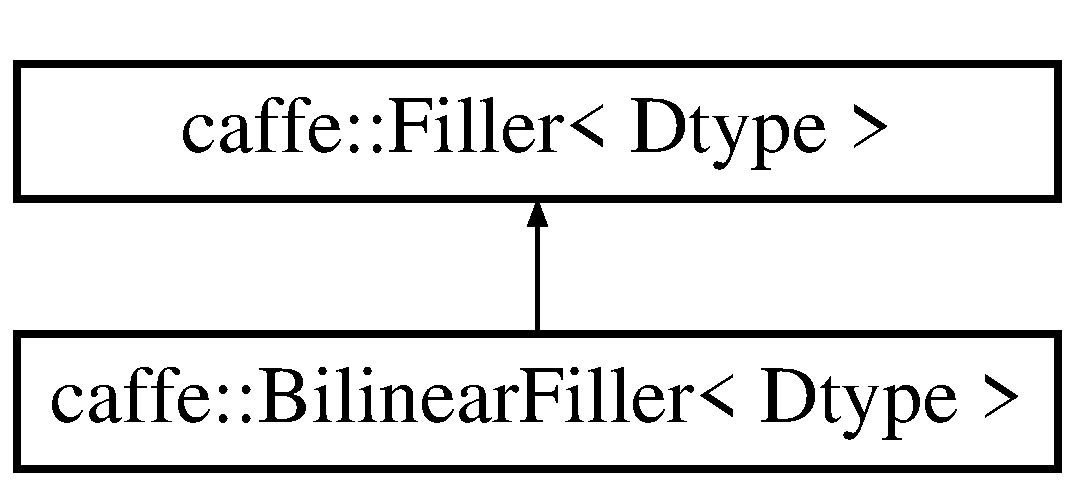
\includegraphics[height=2.000000cm]{classcaffe_1_1BilinearFiller}
\end{center}
\end{figure}
\subsection*{Public Member Functions}
\begin{DoxyCompactItemize}
\item 
{\bfseries Bilinear\+Filler} (const Filler\+Parameter \&param)\hypertarget{classcaffe_1_1BilinearFiller_a5052dabfcc0ba4d5e1514d4e397e21b4}{}\label{classcaffe_1_1BilinearFiller_a5052dabfcc0ba4d5e1514d4e397e21b4}

\item 
virtual void {\bfseries Fill} (\hyperlink{classcaffe_1_1Blob}{Blob}$<$ Dtype $>$ $\ast$blob)\hypertarget{classcaffe_1_1BilinearFiller_a53ddc6c22c21476b9411463b3317418a}{}\label{classcaffe_1_1BilinearFiller_a53ddc6c22c21476b9411463b3317418a}

\end{DoxyCompactItemize}
\subsection*{Additional Inherited Members}


\subsection{Detailed Description}
\subsubsection*{template$<$typename Dtype$>$\\*
class caffe\+::\+Bilinear\+Filler$<$ Dtype $>$}

Fills a \hyperlink{classcaffe_1_1Blob}{Blob} with coefficients for bilinear interpolation. 

A common use case is with the \hyperlink{classcaffe_1_1DeconvolutionLayer}{Deconvolution\+Layer} acting as upsampling. You can upsample a feature map with shape of (B, C, H, W) by any integer factor using the following proto. 
\begin{DoxyCode}
layer \{
  name: \textcolor{stringliteral}{"upsample"}, type: \textcolor{stringliteral}{"Deconvolution"}
  bottom: \textcolor{stringliteral}{"\{\{bottom\_name\}\}"} top: \textcolor{stringliteral}{"\{\{top\_name\}\}"}
  convolution\_param \{
    kernel\_size: \{\{2 * factor - factor % 2\}\} stride: \{\{factor\}\}
    num\_output: \{\{C\}\} group: \{\{C\}\}
    pad: \{\{ceil((factor - 1) / 2.)\}\}
    weight\_filler: \{ type: \textcolor{stringliteral}{"bilinear"} \} bias\_term: \textcolor{keyword}{false}
  \}
  param \{ lr\_mult: 0 decay\_mult: 0 \}
\}
\end{DoxyCode}
 Please use this by replacing {\ttfamily \{\{\}\}} with your values. By specifying {\ttfamily num\+\_\+output\+: \{\{C\}\} group\+: \{\{C\}\}}, it behaves as channel-\/wise convolution. The filter shape of this deconvolution layer will be (C, 1, K, K) where K is {\ttfamily kernel\+\_\+size}, and this filler will set a (K, K) interpolation kernel for every channel of the filter identically. The resulting shape of the top feature map will be (B, C, factor $\ast$ H, factor $\ast$ W). Note that the learning rate and the weight decay are set to 0 in order to keep coefficient values of bilinear interpolation unchanged during training. If you apply this to an image, this operation is equivalent to the following call in Python with Scikit.\+Image. 
\begin{DoxyCode}
1 out = skimage.transform.rescale(img, factor, mode=\textcolor{stringliteral}{'constant'}, cval=0)
\end{DoxyCode}
 

The documentation for this class was generated from the following file\+:\begin{DoxyCompactItemize}
\item 
include/caffe/filler.\+hpp\end{DoxyCompactItemize}

\hypertarget{classcaffe_1_1Blob}{}\section{caffe\+:\+:Blob$<$ Dtype $>$ Class Template Reference}
\label{classcaffe_1_1Blob}\index{caffe\+::\+Blob$<$ Dtype $>$@{caffe\+::\+Blob$<$ Dtype $>$}}


A wrapper around \hyperlink{classcaffe_1_1SyncedMemory}{Synced\+Memory} holders serving as the basic computational unit through which \hyperlink{classcaffe_1_1Layer}{Layer}s, \hyperlink{classcaffe_1_1Net}{Net}s, and \hyperlink{classcaffe_1_1Solver}{Solver}s interact.  




{\ttfamily \#include $<$blob.\+hpp$>$}

\subsection*{Public Member Functions}
\begin{DoxyCompactItemize}
\item 
\hyperlink{classcaffe_1_1Blob_a379df830aad9b3cae253e1ddb0863844}{Blob} (const int \hyperlink{classcaffe_1_1Blob_a56c2b25db397d9e82bbd7c43597ae427}{num}, const int \hyperlink{classcaffe_1_1Blob_a744a987091c4496a2236898ee39558ec}{channels}, const int \hyperlink{classcaffe_1_1Blob_a422a10a605c30ac02a5377e7cf4c8c6c}{height}, const int \hyperlink{classcaffe_1_1Blob_a781b5410b7894455a85cd283cf8ee02a}{width})\hypertarget{classcaffe_1_1Blob_a379df830aad9b3cae253e1ddb0863844}{}\label{classcaffe_1_1Blob_a379df830aad9b3cae253e1ddb0863844}

\begin{DoxyCompactList}\small\item\em Deprecated; use {\ttfamily Blob(const vector$<$int$>$\& shape)}. \end{DoxyCompactList}\item 
{\bfseries Blob} (const vector$<$ int $>$ \&shape)\hypertarget{classcaffe_1_1Blob_a2268ef004df012760d300465a28f0f68}{}\label{classcaffe_1_1Blob_a2268ef004df012760d300465a28f0f68}

\item 
void \hyperlink{classcaffe_1_1Blob_ad0e0a9a4f49478e89161c6afe4e341a0}{Reshape} (const int \hyperlink{classcaffe_1_1Blob_a56c2b25db397d9e82bbd7c43597ae427}{num}, const int \hyperlink{classcaffe_1_1Blob_a744a987091c4496a2236898ee39558ec}{channels}, const int \hyperlink{classcaffe_1_1Blob_a422a10a605c30ac02a5377e7cf4c8c6c}{height}, const int \hyperlink{classcaffe_1_1Blob_a781b5410b7894455a85cd283cf8ee02a}{width})\hypertarget{classcaffe_1_1Blob_ad0e0a9a4f49478e89161c6afe4e341a0}{}\label{classcaffe_1_1Blob_ad0e0a9a4f49478e89161c6afe4e341a0}

\begin{DoxyCompactList}\small\item\em Deprecated; use {\ttfamily \hyperlink{classcaffe_1_1Blob_ac9ce456aa623ff3f4d24225a0db14404}{Reshape(const vector$<$int$>$\& shape)}}. \end{DoxyCompactList}\item 
void \hyperlink{classcaffe_1_1Blob_ac9ce456aa623ff3f4d24225a0db14404}{Reshape} (const vector$<$ int $>$ \&shape)
\begin{DoxyCompactList}\small\item\em Change the dimensions of the blob, allocating new memory if necessary. \end{DoxyCompactList}\item 
void {\bfseries Reshape} (const Blob\+Shape \&shape)\hypertarget{classcaffe_1_1Blob_a787ff5e31db6b53b70fb117002ec0385}{}\label{classcaffe_1_1Blob_a787ff5e31db6b53b70fb117002ec0385}

\item 
void {\bfseries Reshape\+Like} (const \hyperlink{classcaffe_1_1Blob}{Blob} \&other)\hypertarget{classcaffe_1_1Blob_aa8dee739aaa4253f73c44904784ce417}{}\label{classcaffe_1_1Blob_aa8dee739aaa4253f73c44904784ce417}

\item 
string {\bfseries shape\+\_\+string} () const \hypertarget{classcaffe_1_1Blob_a300cd4f89222d01ec5d9826625a0227e}{}\label{classcaffe_1_1Blob_a300cd4f89222d01ec5d9826625a0227e}

\item 
const vector$<$ int $>$ \& {\bfseries shape} () const \hypertarget{classcaffe_1_1Blob_aec8d4b4a44cc0783e9c8333c38226f8f}{}\label{classcaffe_1_1Blob_aec8d4b4a44cc0783e9c8333c38226f8f}

\item 
int \hyperlink{classcaffe_1_1Blob_a3aab16f3e07ddc78e29a101d022a34cd}{shape} (int index) const 
\begin{DoxyCompactList}\small\item\em Returns the dimension of the index-\/th axis (or the negative index-\/th axis from the end, if index is negative). \end{DoxyCompactList}\item 
int {\bfseries num\+\_\+axes} () const \hypertarget{classcaffe_1_1Blob_ab0774eb9e8cd070c7af741b56602f74b}{}\label{classcaffe_1_1Blob_ab0774eb9e8cd070c7af741b56602f74b}

\item 
int {\bfseries count} () const \hypertarget{classcaffe_1_1Blob_abf97753a599dd546c16d55ba926d4e81}{}\label{classcaffe_1_1Blob_abf97753a599dd546c16d55ba926d4e81}

\item 
int \hyperlink{classcaffe_1_1Blob_adcc7936d19ff798cfa8f24901a63d1fa}{count} (int start\+\_\+axis, int end\+\_\+axis) const 
\begin{DoxyCompactList}\small\item\em Compute the volume of a slice; i.\+e., the product of dimensions among a range of axes. \end{DoxyCompactList}\item 
int \hyperlink{classcaffe_1_1Blob_aca6ae30ecc52bd38699fd82fdbe147f7}{count} (int start\+\_\+axis) const 
\begin{DoxyCompactList}\small\item\em Compute the volume of a slice spanning from a particular first axis to the final axis. \end{DoxyCompactList}\item 
int \hyperlink{classcaffe_1_1Blob_a6ce87a58a08438c46a4858929a77ee77}{Canonical\+Axis\+Index} (int axis\+\_\+index) const 
\begin{DoxyCompactList}\small\item\em Returns the \textquotesingle{}canonical\textquotesingle{} version of a (usually) user-\/specified axis, allowing for negative indexing (e.\+g., -\/1 for the last axis). \end{DoxyCompactList}\item 
int \hyperlink{classcaffe_1_1Blob_a56c2b25db397d9e82bbd7c43597ae427}{num} () const \hypertarget{classcaffe_1_1Blob_a56c2b25db397d9e82bbd7c43597ae427}{}\label{classcaffe_1_1Blob_a56c2b25db397d9e82bbd7c43597ae427}

\begin{DoxyCompactList}\small\item\em Deprecated legacy shape accessor num\+: use shape(0) instead. \end{DoxyCompactList}\item 
int \hyperlink{classcaffe_1_1Blob_a744a987091c4496a2236898ee39558ec}{channels} () const \hypertarget{classcaffe_1_1Blob_a744a987091c4496a2236898ee39558ec}{}\label{classcaffe_1_1Blob_a744a987091c4496a2236898ee39558ec}

\begin{DoxyCompactList}\small\item\em Deprecated legacy shape accessor channels\+: use shape(1) instead. \end{DoxyCompactList}\item 
int \hyperlink{classcaffe_1_1Blob_a422a10a605c30ac02a5377e7cf4c8c6c}{height} () const \hypertarget{classcaffe_1_1Blob_a422a10a605c30ac02a5377e7cf4c8c6c}{}\label{classcaffe_1_1Blob_a422a10a605c30ac02a5377e7cf4c8c6c}

\begin{DoxyCompactList}\small\item\em Deprecated legacy shape accessor height\+: use shape(2) instead. \end{DoxyCompactList}\item 
int \hyperlink{classcaffe_1_1Blob_a781b5410b7894455a85cd283cf8ee02a}{width} () const \hypertarget{classcaffe_1_1Blob_a781b5410b7894455a85cd283cf8ee02a}{}\label{classcaffe_1_1Blob_a781b5410b7894455a85cd283cf8ee02a}

\begin{DoxyCompactList}\small\item\em Deprecated legacy shape accessor width\+: use shape(3) instead. \end{DoxyCompactList}\item 
int {\bfseries Legacy\+Shape} (int index) const \hypertarget{classcaffe_1_1Blob_a6221f2df6da6167db15c2b18aac2e5ee}{}\label{classcaffe_1_1Blob_a6221f2df6da6167db15c2b18aac2e5ee}

\item 
int {\bfseries offset} (const int n, const int c=0, const int h=0, const int w=0) const \hypertarget{classcaffe_1_1Blob_a87022dfa6cc45b3a2727ccce9ccf4b2c}{}\label{classcaffe_1_1Blob_a87022dfa6cc45b3a2727ccce9ccf4b2c}

\item 
int {\bfseries offset} (const vector$<$ int $>$ \&indices) const \hypertarget{classcaffe_1_1Blob_a8463d5d004dc97580151c1a4283f00f6}{}\label{classcaffe_1_1Blob_a8463d5d004dc97580151c1a4283f00f6}

\item 
void \hyperlink{classcaffe_1_1Blob_a64ad51f99e88233f43a21a85ebe10284}{Copy\+From} (const \hyperlink{classcaffe_1_1Blob}{Blob}$<$ Dtype $>$ \&source, bool copy\+\_\+diff=false, bool reshape=false)
\begin{DoxyCompactList}\small\item\em Copy from a source \hyperlink{classcaffe_1_1Blob}{Blob}. \end{DoxyCompactList}\item 
Dtype {\bfseries data\+\_\+at} (const int n, const int c, const int h, const int w) const \hypertarget{classcaffe_1_1Blob_a3f12332d9d8a0a5adc12c8c75bbbd335}{}\label{classcaffe_1_1Blob_a3f12332d9d8a0a5adc12c8c75bbbd335}

\item 
Dtype {\bfseries diff\+\_\+at} (const int n, const int c, const int h, const int w) const \hypertarget{classcaffe_1_1Blob_a349ee9442e5ba9736b6ccf12359e776e}{}\label{classcaffe_1_1Blob_a349ee9442e5ba9736b6ccf12359e776e}

\item 
Dtype {\bfseries data\+\_\+at} (const vector$<$ int $>$ \&index) const \hypertarget{classcaffe_1_1Blob_a85a566849633e35492a3dc41d9551731}{}\label{classcaffe_1_1Blob_a85a566849633e35492a3dc41d9551731}

\item 
Dtype {\bfseries diff\+\_\+at} (const vector$<$ int $>$ \&index) const \hypertarget{classcaffe_1_1Blob_ab783abf65ca66df623a8a373de65209b}{}\label{classcaffe_1_1Blob_ab783abf65ca66df623a8a373de65209b}

\item 
const shared\+\_\+ptr$<$ \hyperlink{classcaffe_1_1SyncedMemory}{Synced\+Memory} $>$ \& {\bfseries data} () const \hypertarget{classcaffe_1_1Blob_a09d1435056f21ba9df52cee4d6371087}{}\label{classcaffe_1_1Blob_a09d1435056f21ba9df52cee4d6371087}

\item 
const shared\+\_\+ptr$<$ \hyperlink{classcaffe_1_1SyncedMemory}{Synced\+Memory} $>$ \& {\bfseries diff} () const \hypertarget{classcaffe_1_1Blob_ab7a8c2034a34695fe5f777ff3271e80d}{}\label{classcaffe_1_1Blob_ab7a8c2034a34695fe5f777ff3271e80d}

\item 
const Dtype $\ast$ {\bfseries cpu\+\_\+data} () const \hypertarget{classcaffe_1_1Blob_a490e0b609d0d62dbfc317cbe76aa8fa2}{}\label{classcaffe_1_1Blob_a490e0b609d0d62dbfc317cbe76aa8fa2}

\item 
void {\bfseries set\+\_\+cpu\+\_\+data} (Dtype $\ast$data)\hypertarget{classcaffe_1_1Blob_a5d7d38b157e43ff6a8b8bf94b6815daf}{}\label{classcaffe_1_1Blob_a5d7d38b157e43ff6a8b8bf94b6815daf}

\item 
const int $\ast$ {\bfseries gpu\+\_\+shape} () const \hypertarget{classcaffe_1_1Blob_a16e82cd29e919b116cc8e08af451ab11}{}\label{classcaffe_1_1Blob_a16e82cd29e919b116cc8e08af451ab11}

\item 
const Dtype $\ast$ {\bfseries gpu\+\_\+data} () const \hypertarget{classcaffe_1_1Blob_afd60f6fa2044997149075817991bfc19}{}\label{classcaffe_1_1Blob_afd60f6fa2044997149075817991bfc19}

\item 
void {\bfseries set\+\_\+gpu\+\_\+data} (Dtype $\ast$data)\hypertarget{classcaffe_1_1Blob_ad350de479e172e963f02e8332c800bb7}{}\label{classcaffe_1_1Blob_ad350de479e172e963f02e8332c800bb7}

\item 
const Dtype $\ast$ {\bfseries cpu\+\_\+diff} () const \hypertarget{classcaffe_1_1Blob_a59dc87d97e8a0db8302b142eacb64e10}{}\label{classcaffe_1_1Blob_a59dc87d97e8a0db8302b142eacb64e10}

\item 
const Dtype $\ast$ {\bfseries gpu\+\_\+diff} () const \hypertarget{classcaffe_1_1Blob_aafcc1d137ff67dea2d65824ce67bb21d}{}\label{classcaffe_1_1Blob_aafcc1d137ff67dea2d65824ce67bb21d}

\item 
Dtype $\ast$ {\bfseries mutable\+\_\+cpu\+\_\+data} ()\hypertarget{classcaffe_1_1Blob_ac170c040c34e2e78e7fc0d2ee12cf0ef}{}\label{classcaffe_1_1Blob_ac170c040c34e2e78e7fc0d2ee12cf0ef}

\item 
Dtype $\ast$ {\bfseries mutable\+\_\+gpu\+\_\+data} ()\hypertarget{classcaffe_1_1Blob_abac6bde0521e019df173213af6808e3b}{}\label{classcaffe_1_1Blob_abac6bde0521e019df173213af6808e3b}

\item 
Dtype $\ast$ {\bfseries mutable\+\_\+cpu\+\_\+diff} ()\hypertarget{classcaffe_1_1Blob_a4eb870499aa659a5eee7af622cd92eca}{}\label{classcaffe_1_1Blob_a4eb870499aa659a5eee7af622cd92eca}

\item 
Dtype $\ast$ {\bfseries mutable\+\_\+gpu\+\_\+diff} ()\hypertarget{classcaffe_1_1Blob_a8d230bed098a5ee31559df0b8e2db252}{}\label{classcaffe_1_1Blob_a8d230bed098a5ee31559df0b8e2db252}

\item 
void {\bfseries Update} ()\hypertarget{classcaffe_1_1Blob_afe035d7b60c56e4aed2a18296e8ffdc5}{}\label{classcaffe_1_1Blob_afe035d7b60c56e4aed2a18296e8ffdc5}

\item 
void {\bfseries From\+Proto} (const Blob\+Proto \&proto, bool reshape=true)\hypertarget{classcaffe_1_1Blob_a0a95f882414ba0a11d674b134478476d}{}\label{classcaffe_1_1Blob_a0a95f882414ba0a11d674b134478476d}

\item 
void {\bfseries To\+Proto} (Blob\+Proto $\ast$proto, bool write\+\_\+diff=false) const \hypertarget{classcaffe_1_1Blob_ad297f6b6cad67200c3b5201034653271}{}\label{classcaffe_1_1Blob_ad297f6b6cad67200c3b5201034653271}

\item 
Dtype \hyperlink{classcaffe_1_1Blob_a7ee118b64a34cdb1acb8533d9b68aa64}{asum\+\_\+data} () const \hypertarget{classcaffe_1_1Blob_a7ee118b64a34cdb1acb8533d9b68aa64}{}\label{classcaffe_1_1Blob_a7ee118b64a34cdb1acb8533d9b68aa64}

\begin{DoxyCompactList}\small\item\em Compute the sum of absolute values (L1 norm) of the data. \end{DoxyCompactList}\item 
Dtype \hyperlink{classcaffe_1_1Blob_a7305f3f0b0035d41c95462c0b2dc58c2}{asum\+\_\+diff} () const \hypertarget{classcaffe_1_1Blob_a7305f3f0b0035d41c95462c0b2dc58c2}{}\label{classcaffe_1_1Blob_a7305f3f0b0035d41c95462c0b2dc58c2}

\begin{DoxyCompactList}\small\item\em Compute the sum of absolute values (L1 norm) of the diff. \end{DoxyCompactList}\item 
Dtype \hyperlink{classcaffe_1_1Blob_a51e8e67d0445f9d8fe3d0bea71fd90b3}{sumsq\+\_\+data} () const \hypertarget{classcaffe_1_1Blob_a51e8e67d0445f9d8fe3d0bea71fd90b3}{}\label{classcaffe_1_1Blob_a51e8e67d0445f9d8fe3d0bea71fd90b3}

\begin{DoxyCompactList}\small\item\em Compute the sum of squares (L2 norm squared) of the data. \end{DoxyCompactList}\item 
Dtype \hyperlink{classcaffe_1_1Blob_a599d89dc42801233355b9cfd416e67b7}{sumsq\+\_\+diff} () const \hypertarget{classcaffe_1_1Blob_a599d89dc42801233355b9cfd416e67b7}{}\label{classcaffe_1_1Blob_a599d89dc42801233355b9cfd416e67b7}

\begin{DoxyCompactList}\small\item\em Compute the sum of squares (L2 norm squared) of the diff. \end{DoxyCompactList}\item 
void \hyperlink{classcaffe_1_1Blob_a535dd556e777f2e13b8c7438f40749a0}{scale\+\_\+data} (Dtype scale\+\_\+factor)\hypertarget{classcaffe_1_1Blob_a535dd556e777f2e13b8c7438f40749a0}{}\label{classcaffe_1_1Blob_a535dd556e777f2e13b8c7438f40749a0}

\begin{DoxyCompactList}\small\item\em Scale the blob data by a constant factor. \end{DoxyCompactList}\item 
void \hyperlink{classcaffe_1_1Blob_a6d2d83920d961fff033434347f64a3b0}{scale\+\_\+diff} (Dtype scale\+\_\+factor)\hypertarget{classcaffe_1_1Blob_a6d2d83920d961fff033434347f64a3b0}{}\label{classcaffe_1_1Blob_a6d2d83920d961fff033434347f64a3b0}

\begin{DoxyCompactList}\small\item\em Scale the blob diff by a constant factor. \end{DoxyCompactList}\item 
void \hyperlink{classcaffe_1_1Blob_a8fce5a816a2b9629686db69108610d93}{Share\+Data} (const \hyperlink{classcaffe_1_1Blob}{Blob} \&other)
\begin{DoxyCompactList}\small\item\em Set the data\+\_\+ shared\+\_\+ptr to point to the \hyperlink{classcaffe_1_1SyncedMemory}{Synced\+Memory} holding the data\+\_\+ of \hyperlink{classcaffe_1_1Blob}{Blob} other -- useful in \hyperlink{classcaffe_1_1Layer}{Layer}s which simply perform a copy in their Forward pass. \end{DoxyCompactList}\item 
void \hyperlink{classcaffe_1_1Blob_a004781965b09f94c409cec9a6fc7c35c}{Share\+Diff} (const \hyperlink{classcaffe_1_1Blob}{Blob} \&other)
\begin{DoxyCompactList}\small\item\em Set the diff\+\_\+ shared\+\_\+ptr to point to the \hyperlink{classcaffe_1_1SyncedMemory}{Synced\+Memory} holding the diff\+\_\+ of \hyperlink{classcaffe_1_1Blob}{Blob} other -- useful in \hyperlink{classcaffe_1_1Layer}{Layer}s which simply perform a copy in their Forward pass. \end{DoxyCompactList}\item 
bool {\bfseries Shape\+Equals} (const Blob\+Proto \&other)\hypertarget{classcaffe_1_1Blob_aaf5af1d79ac66f15dd5ebe504b36efcd}{}\label{classcaffe_1_1Blob_aaf5af1d79ac66f15dd5ebe504b36efcd}

\item 
{\footnotesize template$<$$>$ }\\void {\bfseries Update} ()\hypertarget{classcaffe_1_1Blob_a128b3c929b6282d8741543044b81894b}{}\label{classcaffe_1_1Blob_a128b3c929b6282d8741543044b81894b}

\item 
{\footnotesize template$<$$>$ }\\void {\bfseries Update} ()\hypertarget{classcaffe_1_1Blob_a7da970e54e58626753ddd73955164481}{}\label{classcaffe_1_1Blob_a7da970e54e58626753ddd73955164481}

\item 
{\footnotesize template$<$$>$ }\\unsigned int {\bfseries asum\+\_\+data} () const\hypertarget{classcaffe_1_1Blob_aaca009ba67cbcd12c18cf3a766db934f}{}\label{classcaffe_1_1Blob_aaca009ba67cbcd12c18cf3a766db934f}

\item 
{\footnotesize template$<$$>$ }\\int {\bfseries asum\+\_\+data} () const\hypertarget{classcaffe_1_1Blob_a7104c5eb03f4307dd65bb098ad4c1a66}{}\label{classcaffe_1_1Blob_a7104c5eb03f4307dd65bb098ad4c1a66}

\item 
{\footnotesize template$<$$>$ }\\unsigned int {\bfseries asum\+\_\+diff} () const\hypertarget{classcaffe_1_1Blob_aba736c86a9d3bdc798bcc6551725f9a9}{}\label{classcaffe_1_1Blob_aba736c86a9d3bdc798bcc6551725f9a9}

\item 
{\footnotesize template$<$$>$ }\\int {\bfseries asum\+\_\+diff} () const\hypertarget{classcaffe_1_1Blob_a1725a104ce88a7eb466f1d1fb3f9cf95}{}\label{classcaffe_1_1Blob_a1725a104ce88a7eb466f1d1fb3f9cf95}

\item 
{\footnotesize template$<$$>$ }\\unsigned int {\bfseries sumsq\+\_\+data} () const\hypertarget{classcaffe_1_1Blob_acac953b71e67c041755151f78a20405f}{}\label{classcaffe_1_1Blob_acac953b71e67c041755151f78a20405f}

\item 
{\footnotesize template$<$$>$ }\\int {\bfseries sumsq\+\_\+data} () const\hypertarget{classcaffe_1_1Blob_a91285b7a182d4927520b7d1ede18ed20}{}\label{classcaffe_1_1Blob_a91285b7a182d4927520b7d1ede18ed20}

\item 
{\footnotesize template$<$$>$ }\\unsigned int {\bfseries sumsq\+\_\+diff} () const\hypertarget{classcaffe_1_1Blob_a71f00f3e867e4ebccd30fb261f5109a2}{}\label{classcaffe_1_1Blob_a71f00f3e867e4ebccd30fb261f5109a2}

\item 
{\footnotesize template$<$$>$ }\\int {\bfseries sumsq\+\_\+diff} () const\hypertarget{classcaffe_1_1Blob_a4edc021fb188ee25d0113a167858c5ec}{}\label{classcaffe_1_1Blob_a4edc021fb188ee25d0113a167858c5ec}

\item 
{\footnotesize template$<$$>$ }\\void {\bfseries scale\+\_\+data} (unsigned int scale\+\_\+factor)\hypertarget{classcaffe_1_1Blob_af90e5b5950b5002ae75243e988a5cfe2}{}\label{classcaffe_1_1Blob_af90e5b5950b5002ae75243e988a5cfe2}

\item 
{\footnotesize template$<$$>$ }\\void {\bfseries scale\+\_\+data} (int scale\+\_\+factor)\hypertarget{classcaffe_1_1Blob_a99de38dc8933f2f6d410eb9cd05aeaa0}{}\label{classcaffe_1_1Blob_a99de38dc8933f2f6d410eb9cd05aeaa0}

\item 
{\footnotesize template$<$$>$ }\\void {\bfseries scale\+\_\+diff} (unsigned int scale\+\_\+factor)\hypertarget{classcaffe_1_1Blob_aaf182851c1d42c79928e9fc2fd6a652e}{}\label{classcaffe_1_1Blob_aaf182851c1d42c79928e9fc2fd6a652e}

\item 
{\footnotesize template$<$$>$ }\\void {\bfseries scale\+\_\+diff} (int scale\+\_\+factor)\hypertarget{classcaffe_1_1Blob_a8eab6dc0ff159e72845774db6f032918}{}\label{classcaffe_1_1Blob_a8eab6dc0ff159e72845774db6f032918}

\item 
{\footnotesize template$<$$>$ }\\void {\bfseries To\+Proto} (Blob\+Proto $\ast$proto, bool write\+\_\+diff) const\hypertarget{classcaffe_1_1Blob_af20401e9b2ad7c89aa7c77711f653b7a}{}\label{classcaffe_1_1Blob_af20401e9b2ad7c89aa7c77711f653b7a}

\item 
{\footnotesize template$<$$>$ }\\void {\bfseries To\+Proto} (Blob\+Proto $\ast$proto, bool write\+\_\+diff) const\hypertarget{classcaffe_1_1Blob_ae21cbe8230094762001913bdaee472a7}{}\label{classcaffe_1_1Blob_ae21cbe8230094762001913bdaee472a7}

\end{DoxyCompactItemize}
\subsection*{Protected Member Functions}
\begin{DoxyCompactItemize}
\item 
{\bfseries D\+I\+S\+A\+B\+L\+E\+\_\+\+C\+O\+P\+Y\+\_\+\+A\+N\+D\+\_\+\+A\+S\+S\+I\+GN} (\hyperlink{classcaffe_1_1Blob}{Blob})\hypertarget{classcaffe_1_1Blob_a603f1a5472e5fae9ca8fec62f6d5c581}{}\label{classcaffe_1_1Blob_a603f1a5472e5fae9ca8fec62f6d5c581}

\end{DoxyCompactItemize}
\subsection*{Protected Attributes}
\begin{DoxyCompactItemize}
\item 
shared\+\_\+ptr$<$ \hyperlink{classcaffe_1_1SyncedMemory}{Synced\+Memory} $>$ {\bfseries data\+\_\+}\hypertarget{classcaffe_1_1Blob_a5240277a3cea1bc530deca40ca0d0e16}{}\label{classcaffe_1_1Blob_a5240277a3cea1bc530deca40ca0d0e16}

\item 
shared\+\_\+ptr$<$ \hyperlink{classcaffe_1_1SyncedMemory}{Synced\+Memory} $>$ {\bfseries diff\+\_\+}\hypertarget{classcaffe_1_1Blob_a9310f9007aa45e529cb6d69d32dbb80c}{}\label{classcaffe_1_1Blob_a9310f9007aa45e529cb6d69d32dbb80c}

\item 
shared\+\_\+ptr$<$ \hyperlink{classcaffe_1_1SyncedMemory}{Synced\+Memory} $>$ {\bfseries shape\+\_\+data\+\_\+}\hypertarget{classcaffe_1_1Blob_af67df400170ae040ccc680e580b3b578}{}\label{classcaffe_1_1Blob_af67df400170ae040ccc680e580b3b578}

\item 
vector$<$ int $>$ {\bfseries shape\+\_\+}\hypertarget{classcaffe_1_1Blob_a5de50aa2b0e48b52d26ae8fe1c7dca82}{}\label{classcaffe_1_1Blob_a5de50aa2b0e48b52d26ae8fe1c7dca82}

\item 
int {\bfseries count\+\_\+}\hypertarget{classcaffe_1_1Blob_acf06ea13a3a14f77c178a525c35a3ea0}{}\label{classcaffe_1_1Blob_acf06ea13a3a14f77c178a525c35a3ea0}

\item 
int {\bfseries capacity\+\_\+}\hypertarget{classcaffe_1_1Blob_a33b722653651763f4cf07c3658a6de33}{}\label{classcaffe_1_1Blob_a33b722653651763f4cf07c3658a6de33}

\end{DoxyCompactItemize}


\subsection{Detailed Description}
\subsubsection*{template$<$typename Dtype$>$\\*
class caffe\+::\+Blob$<$ Dtype $>$}

A wrapper around \hyperlink{classcaffe_1_1SyncedMemory}{Synced\+Memory} holders serving as the basic computational unit through which \hyperlink{classcaffe_1_1Layer}{Layer}s, \hyperlink{classcaffe_1_1Net}{Net}s, and \hyperlink{classcaffe_1_1Solver}{Solver}s interact. 

T\+O\+D\+O(dox)\+: more thorough description. 

\subsection{Member Function Documentation}
\index{caffe\+::\+Blob@{caffe\+::\+Blob}!Canonical\+Axis\+Index@{Canonical\+Axis\+Index}}
\index{Canonical\+Axis\+Index@{Canonical\+Axis\+Index}!caffe\+::\+Blob@{caffe\+::\+Blob}}
\subsubsection[{\texorpdfstring{Canonical\+Axis\+Index(int axis\+\_\+index) const }{CanonicalAxisIndex(int axis_index) const }}]{\setlength{\rightskip}{0pt plus 5cm}template$<$typename Dtype$>$ int {\bf caffe\+::\+Blob}$<$ Dtype $>$\+::Canonical\+Axis\+Index (
\begin{DoxyParamCaption}
\item[{int}]{axis\+\_\+index}
\end{DoxyParamCaption}
) const\hspace{0.3cm}{\ttfamily [inline]}}\hypertarget{classcaffe_1_1Blob_a6ce87a58a08438c46a4858929a77ee77}{}\label{classcaffe_1_1Blob_a6ce87a58a08438c46a4858929a77ee77}


Returns the \textquotesingle{}canonical\textquotesingle{} version of a (usually) user-\/specified axis, allowing for negative indexing (e.\+g., -\/1 for the last axis). 


\begin{DoxyParams}{Parameters}
{\em axis\+\_\+index} & the axis index. If 0 $<$= index $<$ num\+\_\+axes(), return index. If -\/num\+\_\+axes $<$= index $<$= -\/1, return (num\+\_\+axes() -\/ (-\/index)), e.\+g., the last axis index (num\+\_\+axes() -\/ 1) if index == -\/1, the second to last if index == -\/2, etc. Dies on out of range index. \\
\hline
\end{DoxyParams}
\index{caffe\+::\+Blob@{caffe\+::\+Blob}!Copy\+From@{Copy\+From}}
\index{Copy\+From@{Copy\+From}!caffe\+::\+Blob@{caffe\+::\+Blob}}
\subsubsection[{\texorpdfstring{Copy\+From(const Blob$<$ Dtype $>$ \&source, bool copy\+\_\+diff=false, bool reshape=false)}{CopyFrom(const Blob< Dtype > &source, bool copy_diff=false, bool reshape=false)}}]{\setlength{\rightskip}{0pt plus 5cm}template$<$typename Dtype$>$ void {\bf caffe\+::\+Blob}$<$ Dtype $>$\+::Copy\+From (
\begin{DoxyParamCaption}
\item[{const {\bf Blob}$<$ Dtype $>$ \&}]{source, }
\item[{bool}]{copy\+\_\+diff = {\ttfamily false}, }
\item[{bool}]{reshape = {\ttfamily false}}
\end{DoxyParamCaption}
)}\hypertarget{classcaffe_1_1Blob_a64ad51f99e88233f43a21a85ebe10284}{}\label{classcaffe_1_1Blob_a64ad51f99e88233f43a21a85ebe10284}


Copy from a source \hyperlink{classcaffe_1_1Blob}{Blob}. 


\begin{DoxyParams}{Parameters}
{\em source} & the \hyperlink{classcaffe_1_1Blob}{Blob} to copy from \\
\hline
{\em copy\+\_\+diff} & if false, copy the data; if true, copy the diff \\
\hline
{\em reshape} & if false, require this \hyperlink{classcaffe_1_1Blob}{Blob} to be pre-\/shaped to the shape of other (and die otherwise); if true, Reshape this \hyperlink{classcaffe_1_1Blob}{Blob} to other\textquotesingle{}s shape if necessary \\
\hline
\end{DoxyParams}
\index{caffe\+::\+Blob@{caffe\+::\+Blob}!count@{count}}
\index{count@{count}!caffe\+::\+Blob@{caffe\+::\+Blob}}
\subsubsection[{\texorpdfstring{count(int start\+\_\+axis, int end\+\_\+axis) const }{count(int start_axis, int end_axis) const }}]{\setlength{\rightskip}{0pt plus 5cm}template$<$typename Dtype$>$ int {\bf caffe\+::\+Blob}$<$ Dtype $>$\+::count (
\begin{DoxyParamCaption}
\item[{int}]{start\+\_\+axis, }
\item[{int}]{end\+\_\+axis}
\end{DoxyParamCaption}
) const\hspace{0.3cm}{\ttfamily [inline]}}\hypertarget{classcaffe_1_1Blob_adcc7936d19ff798cfa8f24901a63d1fa}{}\label{classcaffe_1_1Blob_adcc7936d19ff798cfa8f24901a63d1fa}


Compute the volume of a slice; i.\+e., the product of dimensions among a range of axes. 


\begin{DoxyParams}{Parameters}
{\em start\+\_\+axis} & The first axis to include in the slice.\\
\hline
{\em end\+\_\+axis} & The first axis to exclude from the slice. \\
\hline
\end{DoxyParams}
\index{caffe\+::\+Blob@{caffe\+::\+Blob}!count@{count}}
\index{count@{count}!caffe\+::\+Blob@{caffe\+::\+Blob}}
\subsubsection[{\texorpdfstring{count(int start\+\_\+axis) const }{count(int start_axis) const }}]{\setlength{\rightskip}{0pt plus 5cm}template$<$typename Dtype$>$ int {\bf caffe\+::\+Blob}$<$ Dtype $>$\+::count (
\begin{DoxyParamCaption}
\item[{int}]{start\+\_\+axis}
\end{DoxyParamCaption}
) const\hspace{0.3cm}{\ttfamily [inline]}}\hypertarget{classcaffe_1_1Blob_aca6ae30ecc52bd38699fd82fdbe147f7}{}\label{classcaffe_1_1Blob_aca6ae30ecc52bd38699fd82fdbe147f7}


Compute the volume of a slice spanning from a particular first axis to the final axis. 


\begin{DoxyParams}{Parameters}
{\em start\+\_\+axis} & The first axis to include in the slice. \\
\hline
\end{DoxyParams}
\index{caffe\+::\+Blob@{caffe\+::\+Blob}!Reshape@{Reshape}}
\index{Reshape@{Reshape}!caffe\+::\+Blob@{caffe\+::\+Blob}}
\subsubsection[{\texorpdfstring{Reshape(const vector$<$ int $>$ \&shape)}{Reshape(const vector< int > &shape)}}]{\setlength{\rightskip}{0pt plus 5cm}template$<$typename Dtype $>$ void {\bf caffe\+::\+Blob}$<$ Dtype $>$\+::Reshape (
\begin{DoxyParamCaption}
\item[{const vector$<$ int $>$ \&}]{shape}
\end{DoxyParamCaption}
)}\hypertarget{classcaffe_1_1Blob_ac9ce456aa623ff3f4d24225a0db14404}{}\label{classcaffe_1_1Blob_ac9ce456aa623ff3f4d24225a0db14404}


Change the dimensions of the blob, allocating new memory if necessary. 

This function can be called both to create an initial allocation of memory, and to adjust the dimensions of a top blob during \hyperlink{classcaffe_1_1Layer_ad9d391b972c769c0ebee34ca6d1c973e}{Layer\+::\+Reshape} or \hyperlink{classcaffe_1_1Layer_aa5fc9ddb31b58958653372bdaaccde94}{Layer\+::\+Forward}. When changing the size of blob, memory will only be reallocated if sufficient memory does not already exist, and excess memory will never be freed.

Note that reshaping an input blob and immediately calling \hyperlink{classcaffe_1_1Net_a7a1a6d17347106dd1284b1b6d28cb4e9}{Net\+::\+Backward} is an error; either \hyperlink{classcaffe_1_1Net_a6f6cf9d40637f7576828d856bb1b1826}{Net\+::\+Forward} or \hyperlink{classcaffe_1_1Net_a8417af82aa83be45d39aab735bdead1d}{Net\+::\+Reshape} need to be called to propagate the new input shape to higher layers. \index{caffe\+::\+Blob@{caffe\+::\+Blob}!shape@{shape}}
\index{shape@{shape}!caffe\+::\+Blob@{caffe\+::\+Blob}}
\subsubsection[{\texorpdfstring{shape(int index) const }{shape(int index) const }}]{\setlength{\rightskip}{0pt plus 5cm}template$<$typename Dtype$>$ int {\bf caffe\+::\+Blob}$<$ Dtype $>$\+::shape (
\begin{DoxyParamCaption}
\item[{int}]{index}
\end{DoxyParamCaption}
) const\hspace{0.3cm}{\ttfamily [inline]}}\hypertarget{classcaffe_1_1Blob_a3aab16f3e07ddc78e29a101d022a34cd}{}\label{classcaffe_1_1Blob_a3aab16f3e07ddc78e29a101d022a34cd}


Returns the dimension of the index-\/th axis (or the negative index-\/th axis from the end, if index is negative). 


\begin{DoxyParams}{Parameters}
{\em index} & the axis index, which may be negative as it will be \char`\"{}canonicalized\char`\"{} using Canonical\+Axis\+Index. Dies on out of range index. \\
\hline
\end{DoxyParams}
\index{caffe\+::\+Blob@{caffe\+::\+Blob}!Share\+Data@{Share\+Data}}
\index{Share\+Data@{Share\+Data}!caffe\+::\+Blob@{caffe\+::\+Blob}}
\subsubsection[{\texorpdfstring{Share\+Data(const Blob \&other)}{ShareData(const Blob &other)}}]{\setlength{\rightskip}{0pt plus 5cm}template$<$typename Dtype $>$ void {\bf caffe\+::\+Blob}$<$ Dtype $>$\+::Share\+Data (
\begin{DoxyParamCaption}
\item[{const {\bf Blob}$<$ Dtype $>$ \&}]{other}
\end{DoxyParamCaption}
)}\hypertarget{classcaffe_1_1Blob_a8fce5a816a2b9629686db69108610d93}{}\label{classcaffe_1_1Blob_a8fce5a816a2b9629686db69108610d93}


Set the data\+\_\+ shared\+\_\+ptr to point to the \hyperlink{classcaffe_1_1SyncedMemory}{Synced\+Memory} holding the data\+\_\+ of \hyperlink{classcaffe_1_1Blob}{Blob} other -- useful in \hyperlink{classcaffe_1_1Layer}{Layer}s which simply perform a copy in their Forward pass. 

This deallocates the \hyperlink{classcaffe_1_1SyncedMemory}{Synced\+Memory} holding this \hyperlink{classcaffe_1_1Blob}{Blob}\textquotesingle{}s data\+\_\+, as shared\+\_\+ptr calls its destructor when reset with the \char`\"{}=\char`\"{} operator. \index{caffe\+::\+Blob@{caffe\+::\+Blob}!Share\+Diff@{Share\+Diff}}
\index{Share\+Diff@{Share\+Diff}!caffe\+::\+Blob@{caffe\+::\+Blob}}
\subsubsection[{\texorpdfstring{Share\+Diff(const Blob \&other)}{ShareDiff(const Blob &other)}}]{\setlength{\rightskip}{0pt plus 5cm}template$<$typename Dtype $>$ void {\bf caffe\+::\+Blob}$<$ Dtype $>$\+::Share\+Diff (
\begin{DoxyParamCaption}
\item[{const {\bf Blob}$<$ Dtype $>$ \&}]{other}
\end{DoxyParamCaption}
)}\hypertarget{classcaffe_1_1Blob_a004781965b09f94c409cec9a6fc7c35c}{}\label{classcaffe_1_1Blob_a004781965b09f94c409cec9a6fc7c35c}


Set the diff\+\_\+ shared\+\_\+ptr to point to the \hyperlink{classcaffe_1_1SyncedMemory}{Synced\+Memory} holding the diff\+\_\+ of \hyperlink{classcaffe_1_1Blob}{Blob} other -- useful in \hyperlink{classcaffe_1_1Layer}{Layer}s which simply perform a copy in their Forward pass. 

This deallocates the \hyperlink{classcaffe_1_1SyncedMemory}{Synced\+Memory} holding this \hyperlink{classcaffe_1_1Blob}{Blob}\textquotesingle{}s diff\+\_\+, as shared\+\_\+ptr calls its destructor when reset with the \char`\"{}=\char`\"{} operator. 

The documentation for this class was generated from the following files\+:\begin{DoxyCompactItemize}
\item 
include/caffe/blob.\+hpp\item 
src/caffe/blob.\+cpp\end{DoxyCompactItemize}

\hypertarget{classcaffe_1_1BlockingQueue}{}\section{caffe\+:\+:Blocking\+Queue$<$ T $>$ Class Template Reference}
\label{classcaffe_1_1BlockingQueue}\index{caffe\+::\+Blocking\+Queue$<$ T $>$@{caffe\+::\+Blocking\+Queue$<$ T $>$}}
\subsection*{Classes}
\begin{DoxyCompactItemize}
\item 
class \hyperlink{classcaffe_1_1BlockingQueue_1_1sync}{sync}
\end{DoxyCompactItemize}
\subsection*{Public Member Functions}
\begin{DoxyCompactItemize}
\item 
void {\bfseries push} (const T \&t)\hypertarget{classcaffe_1_1BlockingQueue_a44d2dc9d99dfa528daeff70f35293e72}{}\label{classcaffe_1_1BlockingQueue_a44d2dc9d99dfa528daeff70f35293e72}

\item 
bool {\bfseries try\+\_\+pop} (T $\ast$t)\hypertarget{classcaffe_1_1BlockingQueue_aa9da66a1c4f5954f46e207ce3f41bd9b}{}\label{classcaffe_1_1BlockingQueue_aa9da66a1c4f5954f46e207ce3f41bd9b}

\item 
T {\bfseries pop} (const string \&log\+\_\+on\+\_\+wait=\char`\"{}\char`\"{})\hypertarget{classcaffe_1_1BlockingQueue_ac49d1dc517a8d963508225750ce1e80d}{}\label{classcaffe_1_1BlockingQueue_ac49d1dc517a8d963508225750ce1e80d}

\item 
bool {\bfseries try\+\_\+peek} (T $\ast$t)\hypertarget{classcaffe_1_1BlockingQueue_aad3abc02b80d1a544674ac9634fb4ebd}{}\label{classcaffe_1_1BlockingQueue_aad3abc02b80d1a544674ac9634fb4ebd}

\item 
T {\bfseries peek} ()\hypertarget{classcaffe_1_1BlockingQueue_a7e767426fc1deebc6bb4626c3e54964b}{}\label{classcaffe_1_1BlockingQueue_a7e767426fc1deebc6bb4626c3e54964b}

\item 
size\+\_\+t {\bfseries size} () const \hypertarget{classcaffe_1_1BlockingQueue_a4739d1be5e182ae2c4675f60c2d264d8}{}\label{classcaffe_1_1BlockingQueue_a4739d1be5e182ae2c4675f60c2d264d8}

\end{DoxyCompactItemize}
\subsection*{Protected Member Functions}
\begin{DoxyCompactItemize}
\item 
{\bfseries D\+I\+S\+A\+B\+L\+E\+\_\+\+C\+O\+P\+Y\+\_\+\+A\+N\+D\+\_\+\+A\+S\+S\+I\+GN} (\hyperlink{classcaffe_1_1BlockingQueue}{Blocking\+Queue})\hypertarget{classcaffe_1_1BlockingQueue_afbc6f67dfc1571625178b46807e09139}{}\label{classcaffe_1_1BlockingQueue_afbc6f67dfc1571625178b46807e09139}

\end{DoxyCompactItemize}
\subsection*{Protected Attributes}
\begin{DoxyCompactItemize}
\item 
std\+::queue$<$ T $>$ {\bfseries queue\+\_\+}\hypertarget{classcaffe_1_1BlockingQueue_a1e9edbd83dcf94ae3c4aeb7300ae6a5a}{}\label{classcaffe_1_1BlockingQueue_a1e9edbd83dcf94ae3c4aeb7300ae6a5a}

\item 
shared\+\_\+ptr$<$ \hyperlink{classcaffe_1_1BlockingQueue_1_1sync}{sync} $>$ {\bfseries sync\+\_\+}\hypertarget{classcaffe_1_1BlockingQueue_a38023bc1eb798189b7c392d00630be9e}{}\label{classcaffe_1_1BlockingQueue_a38023bc1eb798189b7c392d00630be9e}

\end{DoxyCompactItemize}


The documentation for this class was generated from the following files\+:\begin{DoxyCompactItemize}
\item 
include/caffe/util/blocking\+\_\+queue.\+hpp\item 
src/caffe/util/blocking\+\_\+queue.\+cpp\end{DoxyCompactItemize}

\hypertarget{classcaffe_1_1BNLayer}{}\section{caffe\+:\+:B\+N\+Layer$<$ Dtype $>$ Class Template Reference}
\label{classcaffe_1_1BNLayer}\index{caffe\+::\+B\+N\+Layer$<$ Dtype $>$@{caffe\+::\+B\+N\+Layer$<$ Dtype $>$}}


\hyperlink{classcaffe_1_1Batch}{Batch} normalization the input blob along the channel axis while averaging over the spatial axes.  




{\ttfamily \#include $<$bn\+\_\+layer.\+hpp$>$}

Inheritance diagram for caffe\+:\+:B\+N\+Layer$<$ Dtype $>$\+:\begin{figure}[H]
\begin{center}
\leavevmode
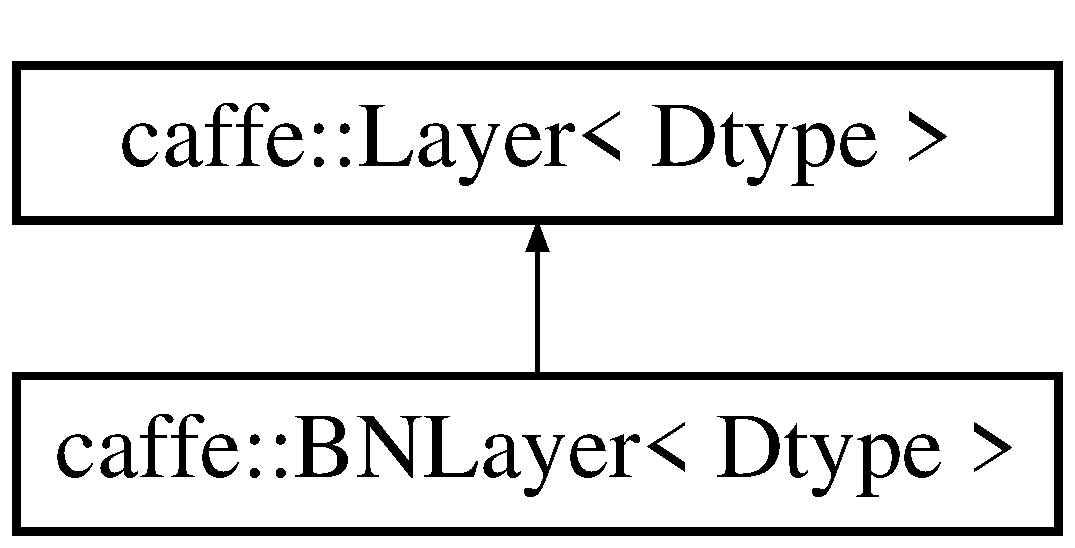
\includegraphics[height=2.000000cm]{classcaffe_1_1BNLayer}
\end{center}
\end{figure}
\subsection*{Public Member Functions}
\begin{DoxyCompactItemize}
\item 
{\bfseries B\+N\+Layer} (const Layer\+Parameter \&param)\hypertarget{classcaffe_1_1BNLayer_ae4fb79c408b580c55d72614768d5f067}{}\label{classcaffe_1_1BNLayer_ae4fb79c408b580c55d72614768d5f067}

\item 
virtual void \hyperlink{classcaffe_1_1BNLayer_aa9d76eb8118c22b13505a7fbbcc68c3f}{Layer\+Set\+Up} (const vector$<$ \hyperlink{classcaffe_1_1Blob}{Blob}$<$ Dtype $>$ $\ast$ $>$ \&bottom, const vector$<$ \hyperlink{classcaffe_1_1Blob}{Blob}$<$ Dtype $>$ $\ast$ $>$ \&top)
\begin{DoxyCompactList}\small\item\em Does layer-\/specific setup\+: your layer should implement this function as well as Reshape. \end{DoxyCompactList}\item 
virtual void \hyperlink{classcaffe_1_1BNLayer_ad925e8d7b344cd6714706d5fe7824c1b}{Reshape} (const vector$<$ \hyperlink{classcaffe_1_1Blob}{Blob}$<$ Dtype $>$ $\ast$ $>$ \&bottom, const vector$<$ \hyperlink{classcaffe_1_1Blob}{Blob}$<$ Dtype $>$ $\ast$ $>$ \&top)
\begin{DoxyCompactList}\small\item\em Adjust the shapes of top blobs and internal buffers to accommodate the shapes of the bottom blobs. \end{DoxyCompactList}\item 
virtual const char $\ast$ \hyperlink{classcaffe_1_1BNLayer_aabf5166f6a6531b756bd4593803cf217}{type} () const \hypertarget{classcaffe_1_1BNLayer_aabf5166f6a6531b756bd4593803cf217}{}\label{classcaffe_1_1BNLayer_aabf5166f6a6531b756bd4593803cf217}

\begin{DoxyCompactList}\small\item\em Returns the layer type. \end{DoxyCompactList}\item 
virtual int \hyperlink{classcaffe_1_1BNLayer_a534fd38c3c24115d5c5676362816157b}{Exact\+Num\+Bottom\+Blobs} () const 
\begin{DoxyCompactList}\small\item\em Returns the exact number of bottom blobs required by the layer, or -\/1 if no exact number is required. \end{DoxyCompactList}\item 
virtual int \hyperlink{classcaffe_1_1BNLayer_a4d608d903ec320429ef155d90aaf9926}{Exact\+Num\+Top\+Blobs} () const 
\begin{DoxyCompactList}\small\item\em Returns the exact number of top blobs required by the layer, or -\/1 if no exact number is required. \end{DoxyCompactList}\end{DoxyCompactItemize}
\subsection*{Protected Member Functions}
\begin{DoxyCompactItemize}
\item 
virtual void \hyperlink{classcaffe_1_1BNLayer_a36989f1535d2354ec8683a1bceda5568}{Forward\+\_\+cpu} (const vector$<$ \hyperlink{classcaffe_1_1Blob}{Blob}$<$ Dtype $>$ $\ast$ $>$ \&bottom, const vector$<$ \hyperlink{classcaffe_1_1Blob}{Blob}$<$ Dtype $>$ $\ast$ $>$ \&top)\hypertarget{classcaffe_1_1BNLayer_a36989f1535d2354ec8683a1bceda5568}{}\label{classcaffe_1_1BNLayer_a36989f1535d2354ec8683a1bceda5568}

\begin{DoxyCompactList}\small\item\em Using the C\+PU device, compute the layer output. \end{DoxyCompactList}\item 
virtual void \hyperlink{classcaffe_1_1BNLayer_a652910518e702bccbe595352e9e50b51}{Forward\+\_\+gpu} (const vector$<$ \hyperlink{classcaffe_1_1Blob}{Blob}$<$ Dtype $>$ $\ast$ $>$ \&bottom, const vector$<$ \hyperlink{classcaffe_1_1Blob}{Blob}$<$ Dtype $>$ $\ast$ $>$ \&top)\hypertarget{classcaffe_1_1BNLayer_a652910518e702bccbe595352e9e50b51}{}\label{classcaffe_1_1BNLayer_a652910518e702bccbe595352e9e50b51}

\begin{DoxyCompactList}\small\item\em Using the G\+PU device, compute the layer output. Fall back to \hyperlink{classcaffe_1_1BNLayer_a36989f1535d2354ec8683a1bceda5568}{Forward\+\_\+cpu()} if unavailable. \end{DoxyCompactList}\item 
virtual void \hyperlink{classcaffe_1_1BNLayer_a87e2372515ba6af62d259a4ec3092c36}{Backward\+\_\+cpu} (const vector$<$ \hyperlink{classcaffe_1_1Blob}{Blob}$<$ Dtype $>$ $\ast$ $>$ \&top, const vector$<$ bool $>$ \&propagate\+\_\+down, const vector$<$ \hyperlink{classcaffe_1_1Blob}{Blob}$<$ Dtype $>$ $\ast$ $>$ \&bottom)\hypertarget{classcaffe_1_1BNLayer_a87e2372515ba6af62d259a4ec3092c36}{}\label{classcaffe_1_1BNLayer_a87e2372515ba6af62d259a4ec3092c36}

\begin{DoxyCompactList}\small\item\em Using the C\+PU device, compute the gradients for any parameters and for the bottom blobs if propagate\+\_\+down is true. \end{DoxyCompactList}\item 
virtual void \hyperlink{classcaffe_1_1BNLayer_ab5c1b118f349d47e4fdc5f9cfddb021f}{Backward\+\_\+gpu} (const vector$<$ \hyperlink{classcaffe_1_1Blob}{Blob}$<$ Dtype $>$ $\ast$ $>$ \&top, const vector$<$ bool $>$ \&propagate\+\_\+down, const vector$<$ \hyperlink{classcaffe_1_1Blob}{Blob}$<$ Dtype $>$ $\ast$ $>$ \&bottom)\hypertarget{classcaffe_1_1BNLayer_ab5c1b118f349d47e4fdc5f9cfddb021f}{}\label{classcaffe_1_1BNLayer_ab5c1b118f349d47e4fdc5f9cfddb021f}

\begin{DoxyCompactList}\small\item\em Using the G\+PU device, compute the gradients for any parameters and for the bottom blobs if propagate\+\_\+down is true. Fall back to \hyperlink{classcaffe_1_1BNLayer_a87e2372515ba6af62d259a4ec3092c36}{Backward\+\_\+cpu()} if unavailable. \end{DoxyCompactList}\item 
void {\bfseries Average\+All\+Except\+Channel} (const Dtype $\ast$input, Dtype $\ast$output)\hypertarget{classcaffe_1_1BNLayer_a99b57558b3db590d6c7b6c2329c81b3b}{}\label{classcaffe_1_1BNLayer_a99b57558b3db590d6c7b6c2329c81b3b}

\item 
void {\bfseries Broadcast\+Channel} (const Dtype $\ast$input, Dtype $\ast$output)\hypertarget{classcaffe_1_1BNLayer_ad01ff398af7bb3b2cfbfa91505b9ef31}{}\label{classcaffe_1_1BNLayer_ad01ff398af7bb3b2cfbfa91505b9ef31}

\end{DoxyCompactItemize}
\subsection*{Protected Attributes}
\begin{DoxyCompactItemize}
\item 
bool {\bfseries frozen\+\_\+}\hypertarget{classcaffe_1_1BNLayer_a398ea207e755b366ab0274ae4104d1fe}{}\label{classcaffe_1_1BNLayer_a398ea207e755b366ab0274ae4104d1fe}

\item 
Dtype {\bfseries bn\+\_\+momentum\+\_\+}\hypertarget{classcaffe_1_1BNLayer_a24b56f9f99fd1c5e6142cdc2ce9770c6}{}\label{classcaffe_1_1BNLayer_a24b56f9f99fd1c5e6142cdc2ce9770c6}

\item 
Dtype {\bfseries bn\+\_\+eps\+\_\+}\hypertarget{classcaffe_1_1BNLayer_aaae0341eafafe018fa7299281684dc89}{}\label{classcaffe_1_1BNLayer_aaae0341eafafe018fa7299281684dc89}

\item 
int {\bfseries num\+\_\+}\hypertarget{classcaffe_1_1BNLayer_a6e3ba8b86eb9ab95371598a734a37f91}{}\label{classcaffe_1_1BNLayer_a6e3ba8b86eb9ab95371598a734a37f91}

\item 
int {\bfseries channels\+\_\+}\hypertarget{classcaffe_1_1BNLayer_a486fafbd71b66558a4a39817a0f81810}{}\label{classcaffe_1_1BNLayer_a486fafbd71b66558a4a39817a0f81810}

\item 
int {\bfseries height\+\_\+}\hypertarget{classcaffe_1_1BNLayer_aac4cacb4c8476a9adbde3fa8e4d33068}{}\label{classcaffe_1_1BNLayer_aac4cacb4c8476a9adbde3fa8e4d33068}

\item 
int {\bfseries width\+\_\+}\hypertarget{classcaffe_1_1BNLayer_a1f9b9a0156f1005ee7c469c48422bc5a}{}\label{classcaffe_1_1BNLayer_a1f9b9a0156f1005ee7c469c48422bc5a}

\item 
\hyperlink{classcaffe_1_1Blob}{Blob}$<$ Dtype $>$ {\bfseries broadcast\+\_\+buffer\+\_\+}\hypertarget{classcaffe_1_1BNLayer_af78d467ce0aa574a61a3c27b0f3e1848}{}\label{classcaffe_1_1BNLayer_af78d467ce0aa574a61a3c27b0f3e1848}

\item 
\hyperlink{classcaffe_1_1Blob}{Blob}$<$ Dtype $>$ {\bfseries spatial\+\_\+statistic\+\_\+}\hypertarget{classcaffe_1_1BNLayer_a08748d7c7984137b8973a1dc424ecc92}{}\label{classcaffe_1_1BNLayer_a08748d7c7984137b8973a1dc424ecc92}

\item 
\hyperlink{classcaffe_1_1Blob}{Blob}$<$ Dtype $>$ {\bfseries batch\+\_\+statistic\+\_\+}\hypertarget{classcaffe_1_1BNLayer_af665ea3902f0001f9fbabb8f0fd87f12}{}\label{classcaffe_1_1BNLayer_af665ea3902f0001f9fbabb8f0fd87f12}

\item 
\hyperlink{classcaffe_1_1Blob}{Blob}$<$ Dtype $>$ {\bfseries x\+\_\+norm\+\_\+}\hypertarget{classcaffe_1_1BNLayer_aa4bb5f65a270d6e6fb18d23a21a0160f}{}\label{classcaffe_1_1BNLayer_aa4bb5f65a270d6e6fb18d23a21a0160f}

\item 
\hyperlink{classcaffe_1_1Blob}{Blob}$<$ Dtype $>$ {\bfseries x\+\_\+inv\+\_\+std\+\_\+}\hypertarget{classcaffe_1_1BNLayer_ac131b1225547fea43443d41276c4b47a}{}\label{classcaffe_1_1BNLayer_ac131b1225547fea43443d41276c4b47a}

\item 
\hyperlink{classcaffe_1_1Blob}{Blob}$<$ Dtype $>$ {\bfseries spatial\+\_\+sum\+\_\+multiplier\+\_\+}\hypertarget{classcaffe_1_1BNLayer_afd96aed6cc5fac07d7c251ba52c0fc76}{}\label{classcaffe_1_1BNLayer_afd96aed6cc5fac07d7c251ba52c0fc76}

\item 
\hyperlink{classcaffe_1_1Blob}{Blob}$<$ Dtype $>$ {\bfseries batch\+\_\+sum\+\_\+multiplier\+\_\+}\hypertarget{classcaffe_1_1BNLayer_a70d55694327c4ac7cc26c11f7f0e193d}{}\label{classcaffe_1_1BNLayer_a70d55694327c4ac7cc26c11f7f0e193d}

\end{DoxyCompactItemize}


\subsection{Detailed Description}
\subsubsection*{template$<$typename Dtype$>$\\*
class caffe\+::\+B\+N\+Layer$<$ Dtype $>$}

\hyperlink{classcaffe_1_1Batch}{Batch} normalization the input blob along the channel axis while averaging over the spatial axes. 

T\+O\+D\+O(dox)\+: thorough documentation for Forward, Backward, and proto params. 

\subsection{Member Function Documentation}
\index{caffe\+::\+B\+N\+Layer@{caffe\+::\+B\+N\+Layer}!Exact\+Num\+Bottom\+Blobs@{Exact\+Num\+Bottom\+Blobs}}
\index{Exact\+Num\+Bottom\+Blobs@{Exact\+Num\+Bottom\+Blobs}!caffe\+::\+B\+N\+Layer@{caffe\+::\+B\+N\+Layer}}
\subsubsection[{\texorpdfstring{Exact\+Num\+Bottom\+Blobs() const }{ExactNumBottomBlobs() const }}]{\setlength{\rightskip}{0pt plus 5cm}template$<$typename Dtype $>$ virtual int {\bf caffe\+::\+B\+N\+Layer}$<$ Dtype $>$\+::Exact\+Num\+Bottom\+Blobs (
\begin{DoxyParamCaption}
{}
\end{DoxyParamCaption}
) const\hspace{0.3cm}{\ttfamily [inline]}, {\ttfamily [virtual]}}\hypertarget{classcaffe_1_1BNLayer_a534fd38c3c24115d5c5676362816157b}{}\label{classcaffe_1_1BNLayer_a534fd38c3c24115d5c5676362816157b}


Returns the exact number of bottom blobs required by the layer, or -\/1 if no exact number is required. 

This method should be overridden to return a non-\/negative value if your layer expects some exact number of bottom blobs. 

Reimplemented from \hyperlink{classcaffe_1_1Layer_a45c7a7943a8a6735ac433c9be11e0240}{caffe\+::\+Layer$<$ Dtype $>$}.

\index{caffe\+::\+B\+N\+Layer@{caffe\+::\+B\+N\+Layer}!Exact\+Num\+Top\+Blobs@{Exact\+Num\+Top\+Blobs}}
\index{Exact\+Num\+Top\+Blobs@{Exact\+Num\+Top\+Blobs}!caffe\+::\+B\+N\+Layer@{caffe\+::\+B\+N\+Layer}}
\subsubsection[{\texorpdfstring{Exact\+Num\+Top\+Blobs() const }{ExactNumTopBlobs() const }}]{\setlength{\rightskip}{0pt plus 5cm}template$<$typename Dtype $>$ virtual int {\bf caffe\+::\+B\+N\+Layer}$<$ Dtype $>$\+::Exact\+Num\+Top\+Blobs (
\begin{DoxyParamCaption}
{}
\end{DoxyParamCaption}
) const\hspace{0.3cm}{\ttfamily [inline]}, {\ttfamily [virtual]}}\hypertarget{classcaffe_1_1BNLayer_a4d608d903ec320429ef155d90aaf9926}{}\label{classcaffe_1_1BNLayer_a4d608d903ec320429ef155d90aaf9926}


Returns the exact number of top blobs required by the layer, or -\/1 if no exact number is required. 

This method should be overridden to return a non-\/negative value if your layer expects some exact number of top blobs. 

Reimplemented from \hyperlink{classcaffe_1_1Layer_aa3c99ed707e8db683a3043412e151af8}{caffe\+::\+Layer$<$ Dtype $>$}.

\index{caffe\+::\+B\+N\+Layer@{caffe\+::\+B\+N\+Layer}!Layer\+Set\+Up@{Layer\+Set\+Up}}
\index{Layer\+Set\+Up@{Layer\+Set\+Up}!caffe\+::\+B\+N\+Layer@{caffe\+::\+B\+N\+Layer}}
\subsubsection[{\texorpdfstring{Layer\+Set\+Up(const vector$<$ Blob$<$ Dtype $>$ $\ast$ $>$ \&bottom, const vector$<$ Blob$<$ Dtype $>$ $\ast$ $>$ \&top)}{LayerSetUp(const vector< Blob< Dtype > * > &bottom, const vector< Blob< Dtype > * > &top)}}]{\setlength{\rightskip}{0pt plus 5cm}template$<$typename Dtype $>$ void {\bf caffe\+::\+B\+N\+Layer}$<$ Dtype $>$\+::Layer\+Set\+Up (
\begin{DoxyParamCaption}
\item[{const vector$<$ {\bf Blob}$<$ Dtype $>$ $\ast$ $>$ \&}]{bottom, }
\item[{const vector$<$ {\bf Blob}$<$ Dtype $>$ $\ast$ $>$ \&}]{top}
\end{DoxyParamCaption}
)\hspace{0.3cm}{\ttfamily [virtual]}}\hypertarget{classcaffe_1_1BNLayer_aa9d76eb8118c22b13505a7fbbcc68c3f}{}\label{classcaffe_1_1BNLayer_aa9d76eb8118c22b13505a7fbbcc68c3f}


Does layer-\/specific setup\+: your layer should implement this function as well as Reshape. 


\begin{DoxyParams}{Parameters}
{\em bottom} & the preshaped input blobs, whose data fields store the input data for this layer \\
\hline
{\em top} & the allocated but unshaped output blobs\\
\hline
\end{DoxyParams}
This method should do one-\/time layer specific setup. This includes reading and processing relevent parameters from the {\ttfamily layer\+\_\+param\+\_\+}. Setting up the shapes of top blobs and internal buffers should be done in {\ttfamily Reshape}, which will be called before the forward pass to adjust the top blob sizes. 

Reimplemented from \hyperlink{classcaffe_1_1Layer_a38dc2488bf319b8de5a7ac84e0045393}{caffe\+::\+Layer$<$ Dtype $>$}.

\index{caffe\+::\+B\+N\+Layer@{caffe\+::\+B\+N\+Layer}!Reshape@{Reshape}}
\index{Reshape@{Reshape}!caffe\+::\+B\+N\+Layer@{caffe\+::\+B\+N\+Layer}}
\subsubsection[{\texorpdfstring{Reshape(const vector$<$ Blob$<$ Dtype $>$ $\ast$ $>$ \&bottom, const vector$<$ Blob$<$ Dtype $>$ $\ast$ $>$ \&top)}{Reshape(const vector< Blob< Dtype > * > &bottom, const vector< Blob< Dtype > * > &top)}}]{\setlength{\rightskip}{0pt plus 5cm}template$<$typename Dtype $>$ void {\bf caffe\+::\+B\+N\+Layer}$<$ Dtype $>$\+::Reshape (
\begin{DoxyParamCaption}
\item[{const vector$<$ {\bf Blob}$<$ Dtype $>$ $\ast$ $>$ \&}]{bottom, }
\item[{const vector$<$ {\bf Blob}$<$ Dtype $>$ $\ast$ $>$ \&}]{top}
\end{DoxyParamCaption}
)\hspace{0.3cm}{\ttfamily [virtual]}}\hypertarget{classcaffe_1_1BNLayer_ad925e8d7b344cd6714706d5fe7824c1b}{}\label{classcaffe_1_1BNLayer_ad925e8d7b344cd6714706d5fe7824c1b}


Adjust the shapes of top blobs and internal buffers to accommodate the shapes of the bottom blobs. 


\begin{DoxyParams}{Parameters}
{\em bottom} & the input blobs, with the requested input shapes \\
\hline
{\em top} & the top blobs, which should be reshaped as needed\\
\hline
\end{DoxyParams}
This method should reshape top blobs as needed according to the shapes of the bottom (input) blobs, as well as reshaping any internal buffers and making any other necessary adjustments so that the layer can accommodate the bottom blobs. 

Implements \hyperlink{classcaffe_1_1Layer_ad9d391b972c769c0ebee34ca6d1c973e}{caffe\+::\+Layer$<$ Dtype $>$}.



The documentation for this class was generated from the following files\+:\begin{DoxyCompactItemize}
\item 
include/caffe/layers/bn\+\_\+layer.\+hpp\item 
src/caffe/layers/bn\+\_\+layer.\+cpp\end{DoxyCompactItemize}

\hypertarget{classcaffe_1_1BNLLLayer}{}\section{caffe\+:\+:B\+N\+L\+L\+Layer$<$ Dtype $>$ Class Template Reference}
\label{classcaffe_1_1BNLLLayer}\index{caffe\+::\+B\+N\+L\+L\+Layer$<$ Dtype $>$@{caffe\+::\+B\+N\+L\+L\+Layer$<$ Dtype $>$}}


Computes $ y = x + \log(1 + \exp(-x)) $ if $ x > 0 $; $ y = \log(1 + \exp(x)) $ otherwise.  




{\ttfamily \#include $<$bnll\+\_\+layer.\+hpp$>$}

Inheritance diagram for caffe\+:\+:B\+N\+L\+L\+Layer$<$ Dtype $>$\+:\begin{figure}[H]
\begin{center}
\leavevmode
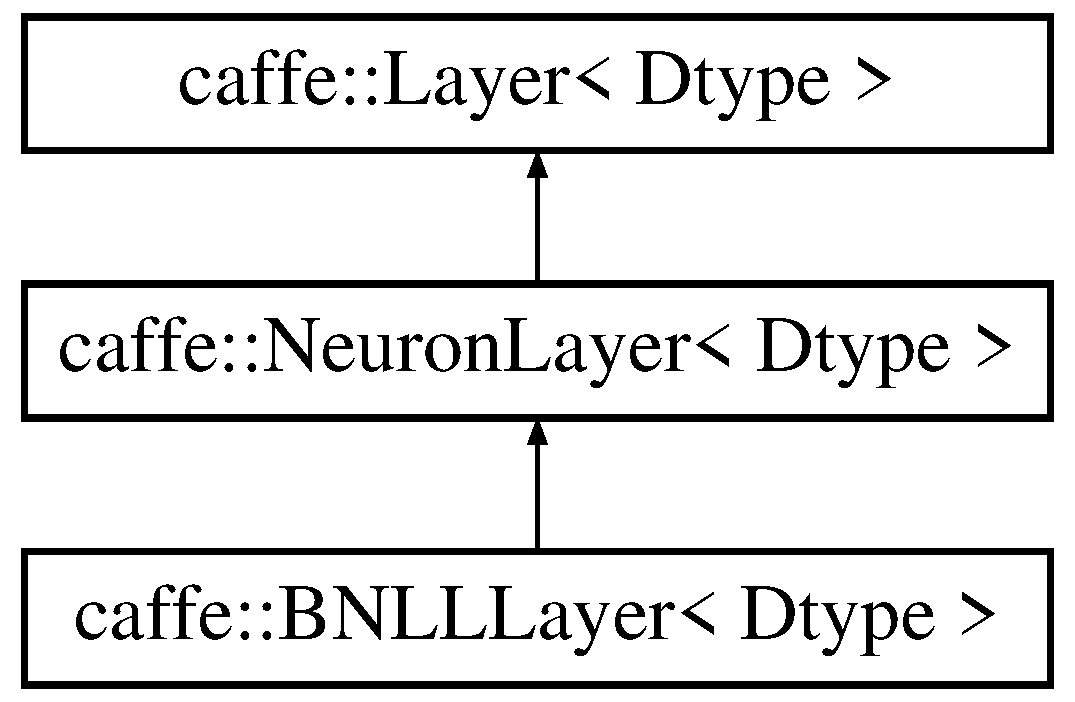
\includegraphics[height=3.000000cm]{classcaffe_1_1BNLLLayer}
\end{center}
\end{figure}
\subsection*{Public Member Functions}
\begin{DoxyCompactItemize}
\item 
{\bfseries B\+N\+L\+L\+Layer} (const Layer\+Parameter \&param)\hypertarget{classcaffe_1_1BNLLLayer_ab30d4b1d22f7489597449e09d74cf4b9}{}\label{classcaffe_1_1BNLLLayer_ab30d4b1d22f7489597449e09d74cf4b9}

\item 
virtual const char $\ast$ \hyperlink{classcaffe_1_1BNLLLayer_a1847167dcb7582eea70e9a5e0d99754a}{type} () const \hypertarget{classcaffe_1_1BNLLLayer_a1847167dcb7582eea70e9a5e0d99754a}{}\label{classcaffe_1_1BNLLLayer_a1847167dcb7582eea70e9a5e0d99754a}

\begin{DoxyCompactList}\small\item\em Returns the layer type. \end{DoxyCompactList}\end{DoxyCompactItemize}
\subsection*{Protected Member Functions}
\begin{DoxyCompactItemize}
\item 
virtual void \hyperlink{classcaffe_1_1BNLLLayer_a6a3458c972d30459aaa46bae3d331ceb}{Forward\+\_\+cpu} (const vector$<$ \hyperlink{classcaffe_1_1Blob}{Blob}$<$ Dtype $>$ $\ast$ $>$ \&bottom, const vector$<$ \hyperlink{classcaffe_1_1Blob}{Blob}$<$ Dtype $>$ $\ast$ $>$ \&top)
\begin{DoxyCompactList}\small\item\em Computes $ y = x + \log(1 + \exp(-x)) $ if $ x > 0 $; $ y = \log(1 + \exp(x)) $ otherwise. \end{DoxyCompactList}\item 
virtual void \hyperlink{classcaffe_1_1BNLLLayer_ab21bef6df27bee7d7579d02c18d8dfb0}{Forward\+\_\+gpu} (const vector$<$ \hyperlink{classcaffe_1_1Blob}{Blob}$<$ Dtype $>$ $\ast$ $>$ \&bottom, const vector$<$ \hyperlink{classcaffe_1_1Blob}{Blob}$<$ Dtype $>$ $\ast$ $>$ \&top)\hypertarget{classcaffe_1_1BNLLLayer_ab21bef6df27bee7d7579d02c18d8dfb0}{}\label{classcaffe_1_1BNLLLayer_ab21bef6df27bee7d7579d02c18d8dfb0}

\begin{DoxyCompactList}\small\item\em Using the G\+PU device, compute the layer output. Fall back to \hyperlink{classcaffe_1_1BNLLLayer_a6a3458c972d30459aaa46bae3d331ceb}{Forward\+\_\+cpu()} if unavailable. \end{DoxyCompactList}\item 
virtual void \hyperlink{classcaffe_1_1BNLLLayer_ab76de68096d3ad4a1ac57ea3dc96f4d1}{Backward\+\_\+cpu} (const vector$<$ \hyperlink{classcaffe_1_1Blob}{Blob}$<$ Dtype $>$ $\ast$ $>$ \&top, const vector$<$ bool $>$ \&propagate\+\_\+down, const vector$<$ \hyperlink{classcaffe_1_1Blob}{Blob}$<$ Dtype $>$ $\ast$ $>$ \&bottom)
\begin{DoxyCompactList}\small\item\em Computes the error gradient w.\+r.\+t. the B\+N\+LL inputs. \end{DoxyCompactList}\item 
virtual void \hyperlink{classcaffe_1_1BNLLLayer_ae85a771b875a4acf2c8b72e51f2da1eb}{Backward\+\_\+gpu} (const vector$<$ \hyperlink{classcaffe_1_1Blob}{Blob}$<$ Dtype $>$ $\ast$ $>$ \&top, const vector$<$ bool $>$ \&propagate\+\_\+down, const vector$<$ \hyperlink{classcaffe_1_1Blob}{Blob}$<$ Dtype $>$ $\ast$ $>$ \&bottom)\hypertarget{classcaffe_1_1BNLLLayer_ae85a771b875a4acf2c8b72e51f2da1eb}{}\label{classcaffe_1_1BNLLLayer_ae85a771b875a4acf2c8b72e51f2da1eb}

\begin{DoxyCompactList}\small\item\em Using the G\+PU device, compute the gradients for any parameters and for the bottom blobs if propagate\+\_\+down is true. Fall back to \hyperlink{classcaffe_1_1BNLLLayer_ab76de68096d3ad4a1ac57ea3dc96f4d1}{Backward\+\_\+cpu()} if unavailable. \end{DoxyCompactList}\end{DoxyCompactItemize}
\subsection*{Additional Inherited Members}


\subsection{Detailed Description}
\subsubsection*{template$<$typename Dtype$>$\\*
class caffe\+::\+B\+N\+L\+L\+Layer$<$ Dtype $>$}

Computes $ y = x + \log(1 + \exp(-x)) $ if $ x > 0 $; $ y = \log(1 + \exp(x)) $ otherwise. 


\begin{DoxyParams}{Parameters}
{\em bottom} & input \hyperlink{classcaffe_1_1Blob}{Blob} vector (length 1)
\begin{DoxyEnumerate}
\item $ (N \times C \times H \times W) $ the inputs $ x $ 
\end{DoxyEnumerate}\\
\hline
{\em top} & output \hyperlink{classcaffe_1_1Blob}{Blob} vector (length 1)
\begin{DoxyEnumerate}
\item $ (N \times C \times H \times W) $ the computed outputs $ y = \left\{ \begin{array}{ll} x + \log(1 + \exp(-x)) & \mbox{if } x > 0 \\ \log(1 + \exp(x)) & \mbox{otherwise} \end{array} \right. $ 
\end{DoxyEnumerate}\\
\hline
\end{DoxyParams}


\subsection{Member Function Documentation}
\index{caffe\+::\+B\+N\+L\+L\+Layer@{caffe\+::\+B\+N\+L\+L\+Layer}!Backward\+\_\+cpu@{Backward\+\_\+cpu}}
\index{Backward\+\_\+cpu@{Backward\+\_\+cpu}!caffe\+::\+B\+N\+L\+L\+Layer@{caffe\+::\+B\+N\+L\+L\+Layer}}
\subsubsection[{\texorpdfstring{Backward\+\_\+cpu(const vector$<$ Blob$<$ Dtype $>$ $\ast$ $>$ \&top, const vector$<$ bool $>$ \&propagate\+\_\+down, const vector$<$ Blob$<$ Dtype $>$ $\ast$ $>$ \&bottom)}{Backward_cpu(const vector< Blob< Dtype > * > &top, const vector< bool > &propagate_down, const vector< Blob< Dtype > * > &bottom)}}]{\setlength{\rightskip}{0pt plus 5cm}template$<$typename Dtype $>$ void {\bf caffe\+::\+B\+N\+L\+L\+Layer}$<$ Dtype $>$\+::Backward\+\_\+cpu (
\begin{DoxyParamCaption}
\item[{const vector$<$ {\bf Blob}$<$ Dtype $>$ $\ast$ $>$ \&}]{top, }
\item[{const vector$<$ bool $>$ \&}]{propagate\+\_\+down, }
\item[{const vector$<$ {\bf Blob}$<$ Dtype $>$ $\ast$ $>$ \&}]{bottom}
\end{DoxyParamCaption}
)\hspace{0.3cm}{\ttfamily [protected]}, {\ttfamily [virtual]}}\hypertarget{classcaffe_1_1BNLLLayer_ab76de68096d3ad4a1ac57ea3dc96f4d1}{}\label{classcaffe_1_1BNLLLayer_ab76de68096d3ad4a1ac57ea3dc96f4d1}


Computes the error gradient w.\+r.\+t. the B\+N\+LL inputs. 


\begin{DoxyParams}{Parameters}
{\em top} & output \hyperlink{classcaffe_1_1Blob}{Blob} vector (length 1), providing the error gradient with respect to the outputs
\begin{DoxyEnumerate}
\item $ (N \times C \times H \times W) $ containing error gradients $ \frac{\partial E}{\partial y} $ with respect to computed outputs $ y $ 
\end{DoxyEnumerate}\\
\hline
{\em propagate\+\_\+down} & see \hyperlink{classcaffe_1_1Layer_a53df1e081767e07bfb4c81657f4acd0a}{Layer\+::\+Backward}. \\
\hline
{\em bottom} & input \hyperlink{classcaffe_1_1Blob}{Blob} vector (length 2)
\begin{DoxyEnumerate}
\item $ (N \times C \times H \times W) $ the inputs $ x $; Backward fills their diff with gradients $ \frac{\partial E}{\partial x} $ if propagate\+\_\+down\mbox{[}0\mbox{]} 
\end{DoxyEnumerate}\\
\hline
\end{DoxyParams}


Implements \hyperlink{classcaffe_1_1Layer_a64d15855f882af4b82e83fa993c4e7c6}{caffe\+::\+Layer$<$ Dtype $>$}.

\index{caffe\+::\+B\+N\+L\+L\+Layer@{caffe\+::\+B\+N\+L\+L\+Layer}!Forward\+\_\+cpu@{Forward\+\_\+cpu}}
\index{Forward\+\_\+cpu@{Forward\+\_\+cpu}!caffe\+::\+B\+N\+L\+L\+Layer@{caffe\+::\+B\+N\+L\+L\+Layer}}
\subsubsection[{\texorpdfstring{Forward\+\_\+cpu(const vector$<$ Blob$<$ Dtype $>$ $\ast$ $>$ \&bottom, const vector$<$ Blob$<$ Dtype $>$ $\ast$ $>$ \&top)}{Forward_cpu(const vector< Blob< Dtype > * > &bottom, const vector< Blob< Dtype > * > &top)}}]{\setlength{\rightskip}{0pt plus 5cm}template$<$typename Dtype $>$ void {\bf caffe\+::\+B\+N\+L\+L\+Layer}$<$ Dtype $>$\+::Forward\+\_\+cpu (
\begin{DoxyParamCaption}
\item[{const vector$<$ {\bf Blob}$<$ Dtype $>$ $\ast$ $>$ \&}]{bottom, }
\item[{const vector$<$ {\bf Blob}$<$ Dtype $>$ $\ast$ $>$ \&}]{top}
\end{DoxyParamCaption}
)\hspace{0.3cm}{\ttfamily [protected]}, {\ttfamily [virtual]}}\hypertarget{classcaffe_1_1BNLLLayer_a6a3458c972d30459aaa46bae3d331ceb}{}\label{classcaffe_1_1BNLLLayer_a6a3458c972d30459aaa46bae3d331ceb}


Computes $ y = x + \log(1 + \exp(-x)) $ if $ x > 0 $; $ y = \log(1 + \exp(x)) $ otherwise. 


\begin{DoxyParams}{Parameters}
{\em bottom} & input \hyperlink{classcaffe_1_1Blob}{Blob} vector (length 1)
\begin{DoxyEnumerate}
\item $ (N \times C \times H \times W) $ the inputs $ x $ 
\end{DoxyEnumerate}\\
\hline
{\em top} & output \hyperlink{classcaffe_1_1Blob}{Blob} vector (length 1)
\begin{DoxyEnumerate}
\item $ (N \times C \times H \times W) $ the computed outputs $ y = \left\{ \begin{array}{ll} x + \log(1 + \exp(-x)) & \mbox{if } x > 0 \\ \log(1 + \exp(x)) & \mbox{otherwise} \end{array} \right. $ 
\end{DoxyEnumerate}\\
\hline
\end{DoxyParams}


Implements \hyperlink{classcaffe_1_1Layer_add965883f75bbf90c7a06f960cda7a1a}{caffe\+::\+Layer$<$ Dtype $>$}.



The documentation for this class was generated from the following files\+:\begin{DoxyCompactItemize}
\item 
include/caffe/layers/bnll\+\_\+layer.\+hpp\item 
src/caffe/layers/bnll\+\_\+layer.\+cpp\end{DoxyCompactItemize}

\hypertarget{classcaffe_1_1Caffe}{}\section{caffe\+:\+:Caffe Class Reference}
\label{classcaffe_1_1Caffe}\index{caffe\+::\+Caffe@{caffe\+::\+Caffe}}
\subsection*{Classes}
\begin{DoxyCompactItemize}
\item 
class \hyperlink{classcaffe_1_1Caffe_1_1RNG}{R\+NG}
\end{DoxyCompactItemize}
\subsection*{Public Types}
\begin{DoxyCompactItemize}
\item 
enum {\bfseries Brew} \{ {\bfseries C\+PU}, 
{\bfseries G\+PU}
 \}\hypertarget{classcaffe_1_1Caffe_af8f607248c1f212be1f6f1c988d80e4e}{}\label{classcaffe_1_1Caffe_af8f607248c1f212be1f6f1c988d80e4e}

\end{DoxyCompactItemize}
\subsection*{Static Public Member Functions}
\begin{DoxyCompactItemize}
\item 
static \hyperlink{classcaffe_1_1Caffe}{Caffe} \& {\bfseries Get} ()\hypertarget{classcaffe_1_1Caffe_a169632a1735728f6bdaacbbe77b81804}{}\label{classcaffe_1_1Caffe_a169632a1735728f6bdaacbbe77b81804}

\item 
static \hyperlink{classcaffe_1_1Caffe_1_1RNG}{R\+NG} \& {\bfseries rng\+\_\+stream} ()\hypertarget{classcaffe_1_1Caffe_aff31f4285d99f4254e2af4e40678bf5e}{}\label{classcaffe_1_1Caffe_aff31f4285d99f4254e2af4e40678bf5e}

\item 
static cublas\+Handle\+\_\+t {\bfseries cublas\+\_\+handle} ()\hypertarget{classcaffe_1_1Caffe_afbba8bb2af70b628eca89269b81c915f}{}\label{classcaffe_1_1Caffe_afbba8bb2af70b628eca89269b81c915f}

\item 
static curand\+Generator\+\_\+t {\bfseries curand\+\_\+generator} ()\hypertarget{classcaffe_1_1Caffe_a659f92f48f20d95c46c6629574a26c0f}{}\label{classcaffe_1_1Caffe_a659f92f48f20d95c46c6629574a26c0f}

\item 
static Brew {\bfseries mode} ()\hypertarget{classcaffe_1_1Caffe_aa45214769b727ecd971e0d5ed8ffe96a}{}\label{classcaffe_1_1Caffe_aa45214769b727ecd971e0d5ed8ffe96a}

\item 
static void {\bfseries set\+\_\+mode} (Brew mode)\hypertarget{classcaffe_1_1Caffe_a025008ff5854ba15e62138c81b7a140d}{}\label{classcaffe_1_1Caffe_a025008ff5854ba15e62138c81b7a140d}

\item 
static void {\bfseries set\+\_\+random\+\_\+seed} (const unsigned int seed)\hypertarget{classcaffe_1_1Caffe_a1f6f560b0f9f73a596284908ee44ecc7}{}\label{classcaffe_1_1Caffe_a1f6f560b0f9f73a596284908ee44ecc7}

\item 
static void {\bfseries Set\+Device} (const int device\+\_\+id)\hypertarget{classcaffe_1_1Caffe_ac95c04832bf528acb3ae8f1ffa5b6c11}{}\label{classcaffe_1_1Caffe_ac95c04832bf528acb3ae8f1ffa5b6c11}

\item 
static void {\bfseries Device\+Query} ()\hypertarget{classcaffe_1_1Caffe_a4af30f25dc929f2b9c1f195e1683a411}{}\label{classcaffe_1_1Caffe_a4af30f25dc929f2b9c1f195e1683a411}

\item 
static bool {\bfseries Check\+Device} (const int device\+\_\+id)\hypertarget{classcaffe_1_1Caffe_ae910c49602d48889673dd614d2aea014}{}\label{classcaffe_1_1Caffe_ae910c49602d48889673dd614d2aea014}

\item 
static int {\bfseries Find\+Device} (const int start\+\_\+id=0)\hypertarget{classcaffe_1_1Caffe_a7ef45036fc831ca416fd1695fc749ea3}{}\label{classcaffe_1_1Caffe_a7ef45036fc831ca416fd1695fc749ea3}

\item 
static int {\bfseries solver\+\_\+count} ()\hypertarget{classcaffe_1_1Caffe_a69e125ae1d6bfa3618fa4d0418d97468}{}\label{classcaffe_1_1Caffe_a69e125ae1d6bfa3618fa4d0418d97468}

\item 
static void {\bfseries set\+\_\+solver\+\_\+count} (int val)\hypertarget{classcaffe_1_1Caffe_ae66753e0dd783b50bbc61c40c89a43f3}{}\label{classcaffe_1_1Caffe_ae66753e0dd783b50bbc61c40c89a43f3}

\item 
static int {\bfseries solver\+\_\+rank} ()\hypertarget{classcaffe_1_1Caffe_abdd6522457e7ac94463d26408620f4c9}{}\label{classcaffe_1_1Caffe_abdd6522457e7ac94463d26408620f4c9}

\item 
static void {\bfseries set\+\_\+solver\+\_\+rank} (int val)\hypertarget{classcaffe_1_1Caffe_a2ec5a171e837fc106e7d1987e3c9a45d}{}\label{classcaffe_1_1Caffe_a2ec5a171e837fc106e7d1987e3c9a45d}

\item 
static bool {\bfseries multiprocess} ()\hypertarget{classcaffe_1_1Caffe_a181e979bf7f7f2fe4a6c5fbbc4d703ac}{}\label{classcaffe_1_1Caffe_a181e979bf7f7f2fe4a6c5fbbc4d703ac}

\item 
static void {\bfseries set\+\_\+multiprocess} (bool val)\hypertarget{classcaffe_1_1Caffe_aea8888baaabfc41014eba175a2538b7b}{}\label{classcaffe_1_1Caffe_aea8888baaabfc41014eba175a2538b7b}

\item 
static bool {\bfseries root\+\_\+solver} ()\hypertarget{classcaffe_1_1Caffe_a87775a1589a6e1b6e53d9bdbb013b8d8}{}\label{classcaffe_1_1Caffe_a87775a1589a6e1b6e53d9bdbb013b8d8}

\end{DoxyCompactItemize}
\subsection*{Protected Attributes}
\begin{DoxyCompactItemize}
\item 
cublas\+Handle\+\_\+t {\bfseries cublas\+\_\+handle\+\_\+}\hypertarget{classcaffe_1_1Caffe_a5fb5298203759722a061644b508ddaeb}{}\label{classcaffe_1_1Caffe_a5fb5298203759722a061644b508ddaeb}

\item 
curand\+Generator\+\_\+t {\bfseries curand\+\_\+generator\+\_\+}\hypertarget{classcaffe_1_1Caffe_a0d920ccea7282d5d88335847c0e9ca9e}{}\label{classcaffe_1_1Caffe_a0d920ccea7282d5d88335847c0e9ca9e}

\item 
shared\+\_\+ptr$<$ \hyperlink{classcaffe_1_1Caffe_1_1RNG}{R\+NG} $>$ {\bfseries random\+\_\+generator\+\_\+}\hypertarget{classcaffe_1_1Caffe_a0c1d6159f6add0ae470af9a09836d979}{}\label{classcaffe_1_1Caffe_a0c1d6159f6add0ae470af9a09836d979}

\item 
Brew {\bfseries mode\+\_\+}\hypertarget{classcaffe_1_1Caffe_aef998c6b69827060630e21a8ccf8884e}{}\label{classcaffe_1_1Caffe_aef998c6b69827060630e21a8ccf8884e}

\item 
int {\bfseries solver\+\_\+count\+\_\+}\hypertarget{classcaffe_1_1Caffe_afc26b38d30812df267645c4a94135a74}{}\label{classcaffe_1_1Caffe_afc26b38d30812df267645c4a94135a74}

\item 
int {\bfseries solver\+\_\+rank\+\_\+}\hypertarget{classcaffe_1_1Caffe_a00152204105cd59b691d8bda828664b5}{}\label{classcaffe_1_1Caffe_a00152204105cd59b691d8bda828664b5}

\item 
bool {\bfseries multiprocess\+\_\+}\hypertarget{classcaffe_1_1Caffe_a25bdfb72baf0bfc5fca31579b08d2b6f}{}\label{classcaffe_1_1Caffe_a25bdfb72baf0bfc5fca31579b08d2b6f}

\end{DoxyCompactItemize}


The documentation for this class was generated from the following files\+:\begin{DoxyCompactItemize}
\item 
include/caffe/common.\+hpp\item 
src/caffe/common.\+cpp\end{DoxyCompactItemize}

\hypertarget{classcaffe_1_1Net_1_1Callback}{}\section{caffe\+:\+:Net$<$ Dtype $>$\+:\+:Callback Class Reference}
\label{classcaffe_1_1Net_1_1Callback}\index{caffe\+::\+Net$<$ Dtype $>$\+::\+Callback@{caffe\+::\+Net$<$ Dtype $>$\+::\+Callback}}
\subsection*{Protected Member Functions}
\begin{DoxyCompactItemize}
\item 
virtual void {\bfseries run} (int layer)=0\hypertarget{classcaffe_1_1Net_1_1Callback_af2a143020f1b44b6da7c95333a364305}{}\label{classcaffe_1_1Net_1_1Callback_af2a143020f1b44b6da7c95333a364305}

\end{DoxyCompactItemize}
\subsection*{Friends}
\begin{DoxyCompactItemize}
\item 
{\footnotesize template$<$typename T $>$ }\\class {\bfseries Net}\hypertarget{classcaffe_1_1Net_1_1Callback_a594f84a944ccdd63ca62bfd4f8623836}{}\label{classcaffe_1_1Net_1_1Callback_a594f84a944ccdd63ca62bfd4f8623836}

\end{DoxyCompactItemize}


The documentation for this class was generated from the following file\+:\begin{DoxyCompactItemize}
\item 
include/caffe/net.\+hpp\end{DoxyCompactItemize}

\hypertarget{classcaffe_1_1Solver_1_1Callback}{}\section{caffe\+:\+:Solver$<$ Dtype $>$\+:\+:Callback Class Reference}
\label{classcaffe_1_1Solver_1_1Callback}\index{caffe\+::\+Solver$<$ Dtype $>$\+::\+Callback@{caffe\+::\+Solver$<$ Dtype $>$\+::\+Callback}}
\subsection*{Protected Member Functions}
\begin{DoxyCompactItemize}
\item 
virtual void {\bfseries on\+\_\+start} ()=0\hypertarget{classcaffe_1_1Solver_1_1Callback_a4af79b534a8323a9fae9d5b0bceb8525}{}\label{classcaffe_1_1Solver_1_1Callback_a4af79b534a8323a9fae9d5b0bceb8525}

\item 
virtual void {\bfseries on\+\_\+gradients\+\_\+ready} ()=0\hypertarget{classcaffe_1_1Solver_1_1Callback_a6c21ab833db14756dde845065752202b}{}\label{classcaffe_1_1Solver_1_1Callback_a6c21ab833db14756dde845065752202b}

\end{DoxyCompactItemize}
\subsection*{Friends}
\begin{DoxyCompactItemize}
\item 
{\footnotesize template$<$typename T $>$ }\\class {\bfseries Solver}\hypertarget{classcaffe_1_1Solver_1_1Callback_a135ddf4017f9df930c2790f5e40d46dc}{}\label{classcaffe_1_1Solver_1_1Callback_a135ddf4017f9df930c2790f5e40d46dc}

\end{DoxyCompactItemize}


The documentation for this class was generated from the following file\+:\begin{DoxyCompactItemize}
\item 
include/caffe/solver.\+hpp\end{DoxyCompactItemize}

\hypertarget{classcaffe_1_1ConcatLayer}{}\section{caffe\+:\+:Concat\+Layer$<$ Dtype $>$ Class Template Reference}
\label{classcaffe_1_1ConcatLayer}\index{caffe\+::\+Concat\+Layer$<$ Dtype $>$@{caffe\+::\+Concat\+Layer$<$ Dtype $>$}}


Takes at least two \hyperlink{classcaffe_1_1Blob}{Blob}s and concatenates them along either the num or channel dimension, outputting the result.  




{\ttfamily \#include $<$concat\+\_\+layer.\+hpp$>$}

Inheritance diagram for caffe\+:\+:Concat\+Layer$<$ Dtype $>$\+:\begin{figure}[H]
\begin{center}
\leavevmode
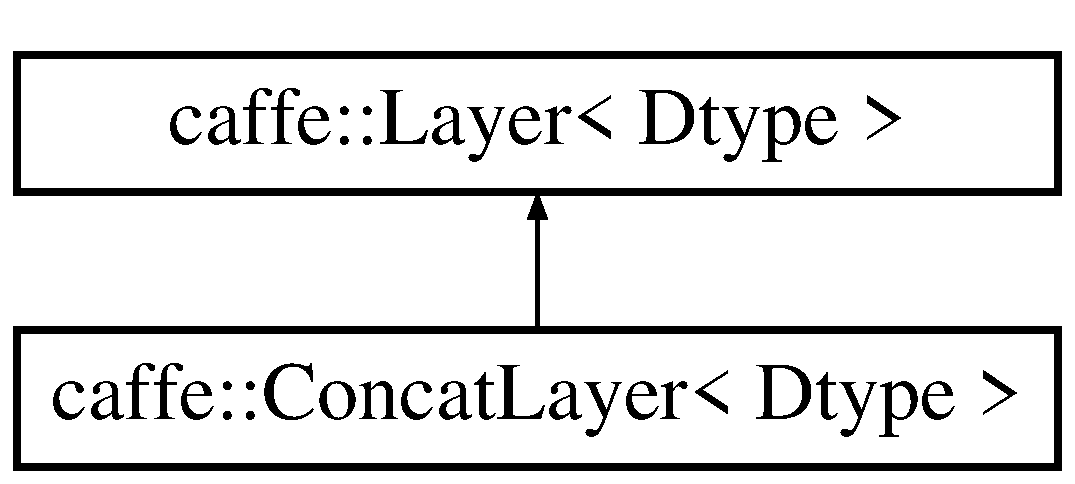
\includegraphics[height=2.000000cm]{classcaffe_1_1ConcatLayer}
\end{center}
\end{figure}
\subsection*{Public Member Functions}
\begin{DoxyCompactItemize}
\item 
{\bfseries Concat\+Layer} (const Layer\+Parameter \&param)\hypertarget{classcaffe_1_1ConcatLayer_aa06930bae7ed23c88546f35323e1792d}{}\label{classcaffe_1_1ConcatLayer_aa06930bae7ed23c88546f35323e1792d}

\item 
virtual void \hyperlink{classcaffe_1_1ConcatLayer_a12555c990bab5fefb25573b3be8a3fbb}{Layer\+Set\+Up} (const vector$<$ \hyperlink{classcaffe_1_1Blob}{Blob}$<$ Dtype $>$ $\ast$ $>$ \&bottom, const vector$<$ \hyperlink{classcaffe_1_1Blob}{Blob}$<$ Dtype $>$ $\ast$ $>$ \&top)
\begin{DoxyCompactList}\small\item\em Does layer-\/specific setup\+: your layer should implement this function as well as Reshape. \end{DoxyCompactList}\item 
virtual void \hyperlink{classcaffe_1_1ConcatLayer_a1bd9d7ac345ea8ac22ff292190d34fc2}{Reshape} (const vector$<$ \hyperlink{classcaffe_1_1Blob}{Blob}$<$ Dtype $>$ $\ast$ $>$ \&bottom, const vector$<$ \hyperlink{classcaffe_1_1Blob}{Blob}$<$ Dtype $>$ $\ast$ $>$ \&top)
\begin{DoxyCompactList}\small\item\em Adjust the shapes of top blobs and internal buffers to accommodate the shapes of the bottom blobs. \end{DoxyCompactList}\item 
virtual const char $\ast$ \hyperlink{classcaffe_1_1ConcatLayer_abf0cda02b061db51e59e56db4c5ce7c8}{type} () const \hypertarget{classcaffe_1_1ConcatLayer_abf0cda02b061db51e59e56db4c5ce7c8}{}\label{classcaffe_1_1ConcatLayer_abf0cda02b061db51e59e56db4c5ce7c8}

\begin{DoxyCompactList}\small\item\em Returns the layer type. \end{DoxyCompactList}\item 
virtual int \hyperlink{classcaffe_1_1ConcatLayer_a5209b379f1c4897414243a155e21602c}{Min\+Bottom\+Blobs} () const 
\begin{DoxyCompactList}\small\item\em Returns the minimum number of bottom blobs required by the layer, or -\/1 if no minimum number is required. \end{DoxyCompactList}\item 
virtual int \hyperlink{classcaffe_1_1ConcatLayer_a3ee6697895b9c39e60b0019eedd7af68}{Exact\+Num\+Top\+Blobs} () const 
\begin{DoxyCompactList}\small\item\em Returns the exact number of top blobs required by the layer, or -\/1 if no exact number is required. \end{DoxyCompactList}\end{DoxyCompactItemize}
\subsection*{Protected Member Functions}
\begin{DoxyCompactItemize}
\item 
virtual void \hyperlink{classcaffe_1_1ConcatLayer_a43e78b577df1365b5a727b607e337dee}{Forward\+\_\+cpu} (const vector$<$ \hyperlink{classcaffe_1_1Blob}{Blob}$<$ Dtype $>$ $\ast$ $>$ \&bottom, const vector$<$ \hyperlink{classcaffe_1_1Blob}{Blob}$<$ Dtype $>$ $\ast$ $>$ \&top)
\item 
virtual void \hyperlink{classcaffe_1_1ConcatLayer_a11543c884c0cc5855048721840bcb3ee}{Forward\+\_\+gpu} (const vector$<$ \hyperlink{classcaffe_1_1Blob}{Blob}$<$ Dtype $>$ $\ast$ $>$ \&bottom, const vector$<$ \hyperlink{classcaffe_1_1Blob}{Blob}$<$ Dtype $>$ $\ast$ $>$ \&top)\hypertarget{classcaffe_1_1ConcatLayer_a11543c884c0cc5855048721840bcb3ee}{}\label{classcaffe_1_1ConcatLayer_a11543c884c0cc5855048721840bcb3ee}

\begin{DoxyCompactList}\small\item\em Using the G\+PU device, compute the layer output. Fall back to \hyperlink{classcaffe_1_1ConcatLayer_a43e78b577df1365b5a727b607e337dee}{Forward\+\_\+cpu()} if unavailable. \end{DoxyCompactList}\item 
virtual void \hyperlink{classcaffe_1_1ConcatLayer_a6c0b0f9d58dfb41657762f02d7dcf466}{Backward\+\_\+cpu} (const vector$<$ \hyperlink{classcaffe_1_1Blob}{Blob}$<$ Dtype $>$ $\ast$ $>$ \&top, const vector$<$ bool $>$ \&propagate\+\_\+down, const vector$<$ \hyperlink{classcaffe_1_1Blob}{Blob}$<$ Dtype $>$ $\ast$ $>$ \&bottom)
\begin{DoxyCompactList}\small\item\em Computes the error gradient w.\+r.\+t. the concatenate inputs. \end{DoxyCompactList}\item 
virtual void \hyperlink{classcaffe_1_1ConcatLayer_aea23ac21d75f019d1db944e15524c548}{Backward\+\_\+gpu} (const vector$<$ \hyperlink{classcaffe_1_1Blob}{Blob}$<$ Dtype $>$ $\ast$ $>$ \&top, const vector$<$ bool $>$ \&propagate\+\_\+down, const vector$<$ \hyperlink{classcaffe_1_1Blob}{Blob}$<$ Dtype $>$ $\ast$ $>$ \&bottom)\hypertarget{classcaffe_1_1ConcatLayer_aea23ac21d75f019d1db944e15524c548}{}\label{classcaffe_1_1ConcatLayer_aea23ac21d75f019d1db944e15524c548}

\begin{DoxyCompactList}\small\item\em Using the G\+PU device, compute the gradients for any parameters and for the bottom blobs if propagate\+\_\+down is true. Fall back to \hyperlink{classcaffe_1_1ConcatLayer_a6c0b0f9d58dfb41657762f02d7dcf466}{Backward\+\_\+cpu()} if unavailable. \end{DoxyCompactList}\end{DoxyCompactItemize}
\subsection*{Protected Attributes}
\begin{DoxyCompactItemize}
\item 
int {\bfseries count\+\_\+}\hypertarget{classcaffe_1_1ConcatLayer_a2e8c2179da287e21df345183f431bd72}{}\label{classcaffe_1_1ConcatLayer_a2e8c2179da287e21df345183f431bd72}

\item 
int {\bfseries num\+\_\+concats\+\_\+}\hypertarget{classcaffe_1_1ConcatLayer_a747feb42310ec1ffdead4cd96008aa8c}{}\label{classcaffe_1_1ConcatLayer_a747feb42310ec1ffdead4cd96008aa8c}

\item 
int {\bfseries concat\+\_\+input\+\_\+size\+\_\+}\hypertarget{classcaffe_1_1ConcatLayer_acdc5e611cf16cbfacfd0d3f08f1ca27f}{}\label{classcaffe_1_1ConcatLayer_acdc5e611cf16cbfacfd0d3f08f1ca27f}

\item 
int {\bfseries concat\+\_\+axis\+\_\+}\hypertarget{classcaffe_1_1ConcatLayer_aaa475cbad6d1e5e681785e69bfc536ff}{}\label{classcaffe_1_1ConcatLayer_aaa475cbad6d1e5e681785e69bfc536ff}

\end{DoxyCompactItemize}


\subsection{Detailed Description}
\subsubsection*{template$<$typename Dtype$>$\\*
class caffe\+::\+Concat\+Layer$<$ Dtype $>$}

Takes at least two \hyperlink{classcaffe_1_1Blob}{Blob}s and concatenates them along either the num or channel dimension, outputting the result. 

\subsection{Member Function Documentation}
\index{caffe\+::\+Concat\+Layer@{caffe\+::\+Concat\+Layer}!Backward\+\_\+cpu@{Backward\+\_\+cpu}}
\index{Backward\+\_\+cpu@{Backward\+\_\+cpu}!caffe\+::\+Concat\+Layer@{caffe\+::\+Concat\+Layer}}
\subsubsection[{\texorpdfstring{Backward\+\_\+cpu(const vector$<$ Blob$<$ Dtype $>$ $\ast$ $>$ \&top, const vector$<$ bool $>$ \&propagate\+\_\+down, const vector$<$ Blob$<$ Dtype $>$ $\ast$ $>$ \&bottom)}{Backward_cpu(const vector< Blob< Dtype > * > &top, const vector< bool > &propagate_down, const vector< Blob< Dtype > * > &bottom)}}]{\setlength{\rightskip}{0pt plus 5cm}template$<$typename Dtype $>$ void {\bf caffe\+::\+Concat\+Layer}$<$ Dtype $>$\+::Backward\+\_\+cpu (
\begin{DoxyParamCaption}
\item[{const vector$<$ {\bf Blob}$<$ Dtype $>$ $\ast$ $>$ \&}]{top, }
\item[{const vector$<$ bool $>$ \&}]{propagate\+\_\+down, }
\item[{const vector$<$ {\bf Blob}$<$ Dtype $>$ $\ast$ $>$ \&}]{bottom}
\end{DoxyParamCaption}
)\hspace{0.3cm}{\ttfamily [protected]}, {\ttfamily [virtual]}}\hypertarget{classcaffe_1_1ConcatLayer_a6c0b0f9d58dfb41657762f02d7dcf466}{}\label{classcaffe_1_1ConcatLayer_a6c0b0f9d58dfb41657762f02d7dcf466}


Computes the error gradient w.\+r.\+t. the concatenate inputs. 


\begin{DoxyParams}{Parameters}
{\em top} & output \hyperlink{classcaffe_1_1Blob}{Blob} vector (length 1), providing the error gradient with respect to the outputs
\begin{DoxyEnumerate}
\item $ (KN \times C \times H \times W) $ if axis == 0, or $ (N \times KC \times H \times W) $ if axis == 1\+: containing error gradients $ \frac{\partial E}{\partial y} $ with respect to concatenated outputs $ y $ 
\end{DoxyEnumerate}\\
\hline
{\em propagate\+\_\+down} & see \hyperlink{classcaffe_1_1Layer_a53df1e081767e07bfb4c81657f4acd0a}{Layer\+::\+Backward}. \\
\hline
{\em bottom} & input \hyperlink{classcaffe_1_1Blob}{Blob} vector (length K), into which the top gradient $ \frac{\partial E}{\partial y} $ is deconcatenated back to the inputs $ \left[ \begin{array}{cccc} \frac{\partial E}{\partial x_1} & \frac{\partial E}{\partial x_2} & ... & \frac{\partial E}{\partial x_K} \end{array} \right] = \frac{\partial E}{\partial y} $ \\
\hline
\end{DoxyParams}


Implements \hyperlink{classcaffe_1_1Layer_a64d15855f882af4b82e83fa993c4e7c6}{caffe\+::\+Layer$<$ Dtype $>$}.

\index{caffe\+::\+Concat\+Layer@{caffe\+::\+Concat\+Layer}!Exact\+Num\+Top\+Blobs@{Exact\+Num\+Top\+Blobs}}
\index{Exact\+Num\+Top\+Blobs@{Exact\+Num\+Top\+Blobs}!caffe\+::\+Concat\+Layer@{caffe\+::\+Concat\+Layer}}
\subsubsection[{\texorpdfstring{Exact\+Num\+Top\+Blobs() const }{ExactNumTopBlobs() const }}]{\setlength{\rightskip}{0pt plus 5cm}template$<$typename Dtype $>$ virtual int {\bf caffe\+::\+Concat\+Layer}$<$ Dtype $>$\+::Exact\+Num\+Top\+Blobs (
\begin{DoxyParamCaption}
{}
\end{DoxyParamCaption}
) const\hspace{0.3cm}{\ttfamily [inline]}, {\ttfamily [virtual]}}\hypertarget{classcaffe_1_1ConcatLayer_a3ee6697895b9c39e60b0019eedd7af68}{}\label{classcaffe_1_1ConcatLayer_a3ee6697895b9c39e60b0019eedd7af68}


Returns the exact number of top blobs required by the layer, or -\/1 if no exact number is required. 

This method should be overridden to return a non-\/negative value if your layer expects some exact number of top blobs. 

Reimplemented from \hyperlink{classcaffe_1_1Layer_aa3c99ed707e8db683a3043412e151af8}{caffe\+::\+Layer$<$ Dtype $>$}.

\index{caffe\+::\+Concat\+Layer@{caffe\+::\+Concat\+Layer}!Forward\+\_\+cpu@{Forward\+\_\+cpu}}
\index{Forward\+\_\+cpu@{Forward\+\_\+cpu}!caffe\+::\+Concat\+Layer@{caffe\+::\+Concat\+Layer}}
\subsubsection[{\texorpdfstring{Forward\+\_\+cpu(const vector$<$ Blob$<$ Dtype $>$ $\ast$ $>$ \&bottom, const vector$<$ Blob$<$ Dtype $>$ $\ast$ $>$ \&top)}{Forward_cpu(const vector< Blob< Dtype > * > &bottom, const vector< Blob< Dtype > * > &top)}}]{\setlength{\rightskip}{0pt plus 5cm}template$<$typename Dtype $>$ void {\bf caffe\+::\+Concat\+Layer}$<$ Dtype $>$\+::Forward\+\_\+cpu (
\begin{DoxyParamCaption}
\item[{const vector$<$ {\bf Blob}$<$ Dtype $>$ $\ast$ $>$ \&}]{bottom, }
\item[{const vector$<$ {\bf Blob}$<$ Dtype $>$ $\ast$ $>$ \&}]{top}
\end{DoxyParamCaption}
)\hspace{0.3cm}{\ttfamily [protected]}, {\ttfamily [virtual]}}\hypertarget{classcaffe_1_1ConcatLayer_a43e78b577df1365b5a727b607e337dee}{}\label{classcaffe_1_1ConcatLayer_a43e78b577df1365b5a727b607e337dee}

\begin{DoxyParams}{Parameters}
{\em bottom} & input \hyperlink{classcaffe_1_1Blob}{Blob} vector (length 2+)
\begin{DoxyEnumerate}
\item $ (N \times C \times H \times W) $ the inputs $ x_1 $
\item $ (N \times C \times H \times W) $ the inputs $ x_2 $
\item ...
\end{DoxyEnumerate}
\begin{DoxyItemize}
\item K $ (N \times C \times H \times W) $ the inputs $ x_K $ 
\end{DoxyItemize}\\
\hline
{\em top} & output \hyperlink{classcaffe_1_1Blob}{Blob} vector (length 1)
\begin{DoxyEnumerate}
\item $ (KN \times C \times H \times W) $ if axis == 0, or $ (N \times KC \times H \times W) $ if axis == 1\+: the concatenated output $ y = [\begin{array}{cccc} x_1 & x_2 & ... & x_K \end{array}] $ 
\end{DoxyEnumerate}\\
\hline
\end{DoxyParams}


Implements \hyperlink{classcaffe_1_1Layer_add965883f75bbf90c7a06f960cda7a1a}{caffe\+::\+Layer$<$ Dtype $>$}.

\index{caffe\+::\+Concat\+Layer@{caffe\+::\+Concat\+Layer}!Layer\+Set\+Up@{Layer\+Set\+Up}}
\index{Layer\+Set\+Up@{Layer\+Set\+Up}!caffe\+::\+Concat\+Layer@{caffe\+::\+Concat\+Layer}}
\subsubsection[{\texorpdfstring{Layer\+Set\+Up(const vector$<$ Blob$<$ Dtype $>$ $\ast$ $>$ \&bottom, const vector$<$ Blob$<$ Dtype $>$ $\ast$ $>$ \&top)}{LayerSetUp(const vector< Blob< Dtype > * > &bottom, const vector< Blob< Dtype > * > &top)}}]{\setlength{\rightskip}{0pt plus 5cm}template$<$typename Dtype $>$ void {\bf caffe\+::\+Concat\+Layer}$<$ Dtype $>$\+::Layer\+Set\+Up (
\begin{DoxyParamCaption}
\item[{const vector$<$ {\bf Blob}$<$ Dtype $>$ $\ast$ $>$ \&}]{bottom, }
\item[{const vector$<$ {\bf Blob}$<$ Dtype $>$ $\ast$ $>$ \&}]{top}
\end{DoxyParamCaption}
)\hspace{0.3cm}{\ttfamily [virtual]}}\hypertarget{classcaffe_1_1ConcatLayer_a12555c990bab5fefb25573b3be8a3fbb}{}\label{classcaffe_1_1ConcatLayer_a12555c990bab5fefb25573b3be8a3fbb}


Does layer-\/specific setup\+: your layer should implement this function as well as Reshape. 


\begin{DoxyParams}{Parameters}
{\em bottom} & the preshaped input blobs, whose data fields store the input data for this layer \\
\hline
{\em top} & the allocated but unshaped output blobs\\
\hline
\end{DoxyParams}
This method should do one-\/time layer specific setup. This includes reading and processing relevent parameters from the {\ttfamily layer\+\_\+param\+\_\+}. Setting up the shapes of top blobs and internal buffers should be done in {\ttfamily Reshape}, which will be called before the forward pass to adjust the top blob sizes. 

Reimplemented from \hyperlink{classcaffe_1_1Layer_a38dc2488bf319b8de5a7ac84e0045393}{caffe\+::\+Layer$<$ Dtype $>$}.

\index{caffe\+::\+Concat\+Layer@{caffe\+::\+Concat\+Layer}!Min\+Bottom\+Blobs@{Min\+Bottom\+Blobs}}
\index{Min\+Bottom\+Blobs@{Min\+Bottom\+Blobs}!caffe\+::\+Concat\+Layer@{caffe\+::\+Concat\+Layer}}
\subsubsection[{\texorpdfstring{Min\+Bottom\+Blobs() const }{MinBottomBlobs() const }}]{\setlength{\rightskip}{0pt plus 5cm}template$<$typename Dtype $>$ virtual int {\bf caffe\+::\+Concat\+Layer}$<$ Dtype $>$\+::Min\+Bottom\+Blobs (
\begin{DoxyParamCaption}
{}
\end{DoxyParamCaption}
) const\hspace{0.3cm}{\ttfamily [inline]}, {\ttfamily [virtual]}}\hypertarget{classcaffe_1_1ConcatLayer_a5209b379f1c4897414243a155e21602c}{}\label{classcaffe_1_1ConcatLayer_a5209b379f1c4897414243a155e21602c}


Returns the minimum number of bottom blobs required by the layer, or -\/1 if no minimum number is required. 

This method should be overridden to return a non-\/negative value if your layer expects some minimum number of bottom blobs. 

Reimplemented from \hyperlink{classcaffe_1_1Layer_ade3eee97cc743c4e68fff7eba6484916}{caffe\+::\+Layer$<$ Dtype $>$}.

\index{caffe\+::\+Concat\+Layer@{caffe\+::\+Concat\+Layer}!Reshape@{Reshape}}
\index{Reshape@{Reshape}!caffe\+::\+Concat\+Layer@{caffe\+::\+Concat\+Layer}}
\subsubsection[{\texorpdfstring{Reshape(const vector$<$ Blob$<$ Dtype $>$ $\ast$ $>$ \&bottom, const vector$<$ Blob$<$ Dtype $>$ $\ast$ $>$ \&top)}{Reshape(const vector< Blob< Dtype > * > &bottom, const vector< Blob< Dtype > * > &top)}}]{\setlength{\rightskip}{0pt plus 5cm}template$<$typename Dtype $>$ void {\bf caffe\+::\+Concat\+Layer}$<$ Dtype $>$\+::Reshape (
\begin{DoxyParamCaption}
\item[{const vector$<$ {\bf Blob}$<$ Dtype $>$ $\ast$ $>$ \&}]{bottom, }
\item[{const vector$<$ {\bf Blob}$<$ Dtype $>$ $\ast$ $>$ \&}]{top}
\end{DoxyParamCaption}
)\hspace{0.3cm}{\ttfamily [virtual]}}\hypertarget{classcaffe_1_1ConcatLayer_a1bd9d7ac345ea8ac22ff292190d34fc2}{}\label{classcaffe_1_1ConcatLayer_a1bd9d7ac345ea8ac22ff292190d34fc2}


Adjust the shapes of top blobs and internal buffers to accommodate the shapes of the bottom blobs. 


\begin{DoxyParams}{Parameters}
{\em bottom} & the input blobs, with the requested input shapes \\
\hline
{\em top} & the top blobs, which should be reshaped as needed\\
\hline
\end{DoxyParams}
This method should reshape top blobs as needed according to the shapes of the bottom (input) blobs, as well as reshaping any internal buffers and making any other necessary adjustments so that the layer can accommodate the bottom blobs. 

Implements \hyperlink{classcaffe_1_1Layer_ad9d391b972c769c0ebee34ca6d1c973e}{caffe\+::\+Layer$<$ Dtype $>$}.



The documentation for this class was generated from the following files\+:\begin{DoxyCompactItemize}
\item 
include/caffe/layers/concat\+\_\+layer.\+hpp\item 
src/caffe/layers/concat\+\_\+layer.\+cpp\end{DoxyCompactItemize}

\hypertarget{classcaffe_1_1ConstantFiller}{}\section{caffe\+:\+:Constant\+Filler$<$ Dtype $>$ Class Template Reference}
\label{classcaffe_1_1ConstantFiller}\index{caffe\+::\+Constant\+Filler$<$ Dtype $>$@{caffe\+::\+Constant\+Filler$<$ Dtype $>$}}


Fills a \hyperlink{classcaffe_1_1Blob}{Blob} with constant values $ x = 0 $.  




{\ttfamily \#include $<$filler.\+hpp$>$}

Inheritance diagram for caffe\+:\+:Constant\+Filler$<$ Dtype $>$\+:\begin{figure}[H]
\begin{center}
\leavevmode
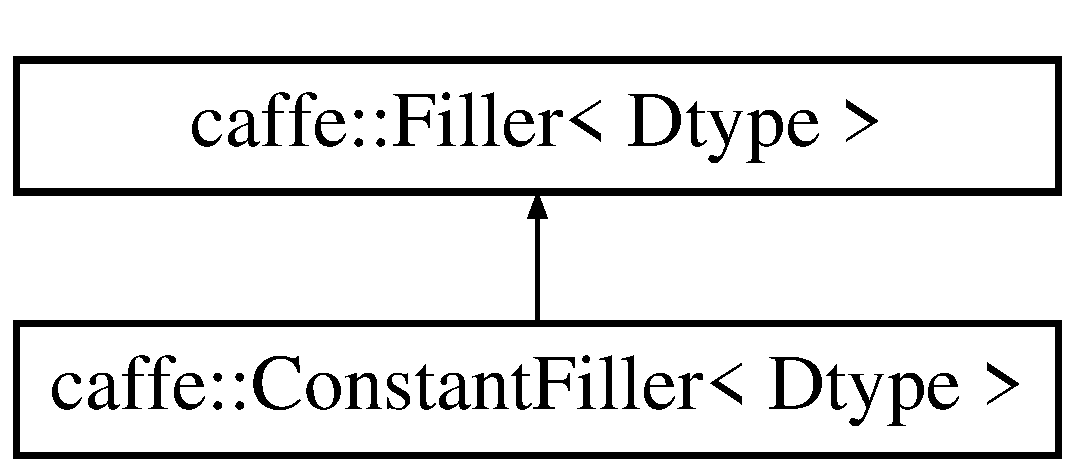
\includegraphics[height=2.000000cm]{classcaffe_1_1ConstantFiller}
\end{center}
\end{figure}
\subsection*{Public Member Functions}
\begin{DoxyCompactItemize}
\item 
{\bfseries Constant\+Filler} (const Filler\+Parameter \&param)\hypertarget{classcaffe_1_1ConstantFiller_ac6bd25bc764935cb5261d0279a772001}{}\label{classcaffe_1_1ConstantFiller_ac6bd25bc764935cb5261d0279a772001}

\item 
virtual void {\bfseries Fill} (\hyperlink{classcaffe_1_1Blob}{Blob}$<$ Dtype $>$ $\ast$blob)\hypertarget{classcaffe_1_1ConstantFiller_a411cf44b177109c388c0b34c906f4e8e}{}\label{classcaffe_1_1ConstantFiller_a411cf44b177109c388c0b34c906f4e8e}

\end{DoxyCompactItemize}
\subsection*{Additional Inherited Members}


\subsection{Detailed Description}
\subsubsection*{template$<$typename Dtype$>$\\*
class caffe\+::\+Constant\+Filler$<$ Dtype $>$}

Fills a \hyperlink{classcaffe_1_1Blob}{Blob} with constant values $ x = 0 $. 

The documentation for this class was generated from the following file\+:\begin{DoxyCompactItemize}
\item 
include/caffe/filler.\+hpp\end{DoxyCompactItemize}

\hypertarget{classcaffe_1_1ContrastiveLossLayer}{}\section{caffe\+:\+:Contrastive\+Loss\+Layer$<$ Dtype $>$ Class Template Reference}
\label{classcaffe_1_1ContrastiveLossLayer}\index{caffe\+::\+Contrastive\+Loss\+Layer$<$ Dtype $>$@{caffe\+::\+Contrastive\+Loss\+Layer$<$ Dtype $>$}}


Computes the contrastive loss $ E = \frac{1}{2N} \sum\limits_{n=1}^N \left(y\right) d^2 + \left(1-y\right) \max \left(margin-d, 0\right)^2 $ where $ d = \left| \left| a_n - b_n \right| \right|_2 $. This can be used to train siamese networks.  




{\ttfamily \#include $<$contrastive\+\_\+loss\+\_\+layer.\+hpp$>$}

Inheritance diagram for caffe\+:\+:Contrastive\+Loss\+Layer$<$ Dtype $>$\+:\begin{figure}[H]
\begin{center}
\leavevmode
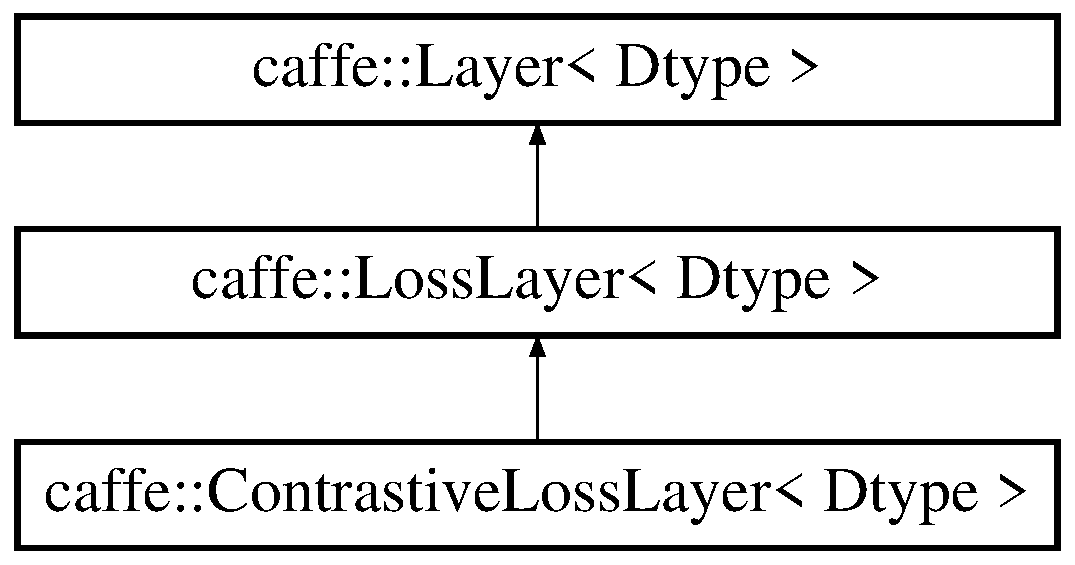
\includegraphics[height=3.000000cm]{classcaffe_1_1ContrastiveLossLayer}
\end{center}
\end{figure}
\subsection*{Public Member Functions}
\begin{DoxyCompactItemize}
\item 
{\bfseries Contrastive\+Loss\+Layer} (const Layer\+Parameter \&param)\hypertarget{classcaffe_1_1ContrastiveLossLayer_aab41120fe462451196d14321264aef60}{}\label{classcaffe_1_1ContrastiveLossLayer_aab41120fe462451196d14321264aef60}

\item 
virtual void \hyperlink{classcaffe_1_1ContrastiveLossLayer_a34a16b3e6598ec6c23e63c01ef0c0a99}{Layer\+Set\+Up} (const vector$<$ \hyperlink{classcaffe_1_1Blob}{Blob}$<$ Dtype $>$ $\ast$ $>$ \&bottom, const vector$<$ \hyperlink{classcaffe_1_1Blob}{Blob}$<$ Dtype $>$ $\ast$ $>$ \&top)
\begin{DoxyCompactList}\small\item\em Does layer-\/specific setup\+: your layer should implement this function as well as Reshape. \end{DoxyCompactList}\item 
virtual int \hyperlink{classcaffe_1_1ContrastiveLossLayer_af1b8bcaf8ddacd3e98e26c558c7f49a0}{Exact\+Num\+Bottom\+Blobs} () const 
\begin{DoxyCompactList}\small\item\em Returns the exact number of bottom blobs required by the layer, or -\/1 if no exact number is required. \end{DoxyCompactList}\item 
virtual const char $\ast$ \hyperlink{classcaffe_1_1ContrastiveLossLayer_a34b18bace2b4419132d1364516da19f6}{type} () const \hypertarget{classcaffe_1_1ContrastiveLossLayer_a34b18bace2b4419132d1364516da19f6}{}\label{classcaffe_1_1ContrastiveLossLayer_a34b18bace2b4419132d1364516da19f6}

\begin{DoxyCompactList}\small\item\em Returns the layer type. \end{DoxyCompactList}\item 
virtual bool \hyperlink{classcaffe_1_1ContrastiveLossLayer_afbfe9d1707c9e76e31fe381af3d708ef}{Allow\+Force\+Backward} (const int bottom\+\_\+index) const 
\end{DoxyCompactItemize}
\subsection*{Protected Member Functions}
\begin{DoxyCompactItemize}
\item 
virtual void \hyperlink{classcaffe_1_1ContrastiveLossLayer_a0719301088807da84f30ef2f028d0fde}{Forward\+\_\+cpu} (const vector$<$ \hyperlink{classcaffe_1_1Blob}{Blob}$<$ Dtype $>$ $\ast$ $>$ \&bottom, const vector$<$ \hyperlink{classcaffe_1_1Blob}{Blob}$<$ Dtype $>$ $\ast$ $>$ \&top)
\begin{DoxyCompactList}\small\item\em Computes the contrastive loss $ E = \frac{1}{2N} \sum\limits_{n=1}^N \left(y\right) d^2 + \left(1-y\right) \max \left(margin-d, 0\right)^2 $ where $ d = \left| \left| a_n - b_n \right| \right|_2 $. This can be used to train siamese networks. \end{DoxyCompactList}\item 
virtual void \hyperlink{classcaffe_1_1ContrastiveLossLayer_acc9c79ec2883380d41308c8212d0f845}{Forward\+\_\+gpu} (const vector$<$ \hyperlink{classcaffe_1_1Blob}{Blob}$<$ Dtype $>$ $\ast$ $>$ \&bottom, const vector$<$ \hyperlink{classcaffe_1_1Blob}{Blob}$<$ Dtype $>$ $\ast$ $>$ \&top)\hypertarget{classcaffe_1_1ContrastiveLossLayer_acc9c79ec2883380d41308c8212d0f845}{}\label{classcaffe_1_1ContrastiveLossLayer_acc9c79ec2883380d41308c8212d0f845}

\begin{DoxyCompactList}\small\item\em Using the G\+PU device, compute the layer output. Fall back to \hyperlink{classcaffe_1_1ContrastiveLossLayer_a0719301088807da84f30ef2f028d0fde}{Forward\+\_\+cpu()} if unavailable. \end{DoxyCompactList}\item 
virtual void \hyperlink{classcaffe_1_1ContrastiveLossLayer_ac29d021f30dbab75ca14cb79446926e5}{Backward\+\_\+cpu} (const vector$<$ \hyperlink{classcaffe_1_1Blob}{Blob}$<$ Dtype $>$ $\ast$ $>$ \&top, const vector$<$ bool $>$ \&propagate\+\_\+down, const vector$<$ \hyperlink{classcaffe_1_1Blob}{Blob}$<$ Dtype $>$ $\ast$ $>$ \&bottom)
\begin{DoxyCompactList}\small\item\em Computes the Contrastive error gradient w.\+r.\+t. the inputs. \end{DoxyCompactList}\item 
virtual void \hyperlink{classcaffe_1_1ContrastiveLossLayer_abdafac096cf9ba58eff8fe0621f0275a}{Backward\+\_\+gpu} (const vector$<$ \hyperlink{classcaffe_1_1Blob}{Blob}$<$ Dtype $>$ $\ast$ $>$ \&top, const vector$<$ bool $>$ \&propagate\+\_\+down, const vector$<$ \hyperlink{classcaffe_1_1Blob}{Blob}$<$ Dtype $>$ $\ast$ $>$ \&bottom)\hypertarget{classcaffe_1_1ContrastiveLossLayer_abdafac096cf9ba58eff8fe0621f0275a}{}\label{classcaffe_1_1ContrastiveLossLayer_abdafac096cf9ba58eff8fe0621f0275a}

\begin{DoxyCompactList}\small\item\em Using the G\+PU device, compute the gradients for any parameters and for the bottom blobs if propagate\+\_\+down is true. Fall back to \hyperlink{classcaffe_1_1ContrastiveLossLayer_ac29d021f30dbab75ca14cb79446926e5}{Backward\+\_\+cpu()} if unavailable. \end{DoxyCompactList}\end{DoxyCompactItemize}
\subsection*{Protected Attributes}
\begin{DoxyCompactItemize}
\item 
\hyperlink{classcaffe_1_1Blob}{Blob}$<$ Dtype $>$ {\bfseries diff\+\_\+}\hypertarget{classcaffe_1_1ContrastiveLossLayer_a885617ad377571b4010d8a39f0a53d5e}{}\label{classcaffe_1_1ContrastiveLossLayer_a885617ad377571b4010d8a39f0a53d5e}

\item 
\hyperlink{classcaffe_1_1Blob}{Blob}$<$ Dtype $>$ {\bfseries dist\+\_\+sq\+\_\+}\hypertarget{classcaffe_1_1ContrastiveLossLayer_ab852b524ed8daee905f2f0eeddfb9807}{}\label{classcaffe_1_1ContrastiveLossLayer_ab852b524ed8daee905f2f0eeddfb9807}

\item 
\hyperlink{classcaffe_1_1Blob}{Blob}$<$ Dtype $>$ {\bfseries diff\+\_\+sq\+\_\+}\hypertarget{classcaffe_1_1ContrastiveLossLayer_a2e73f7304a21d8e265b6389c9e7095e6}{}\label{classcaffe_1_1ContrastiveLossLayer_a2e73f7304a21d8e265b6389c9e7095e6}

\item 
\hyperlink{classcaffe_1_1Blob}{Blob}$<$ Dtype $>$ {\bfseries summer\+\_\+vec\+\_\+}\hypertarget{classcaffe_1_1ContrastiveLossLayer_a7b67d18ffc05ea6acce6b8c1c2de82a4}{}\label{classcaffe_1_1ContrastiveLossLayer_a7b67d18ffc05ea6acce6b8c1c2de82a4}

\end{DoxyCompactItemize}


\subsection{Detailed Description}
\subsubsection*{template$<$typename Dtype$>$\\*
class caffe\+::\+Contrastive\+Loss\+Layer$<$ Dtype $>$}

Computes the contrastive loss $ E = \frac{1}{2N} \sum\limits_{n=1}^N \left(y\right) d^2 + \left(1-y\right) \max \left(margin-d, 0\right)^2 $ where $ d = \left| \left| a_n - b_n \right| \right|_2 $. This can be used to train siamese networks. 


\begin{DoxyParams}{Parameters}
{\em bottom} & input \hyperlink{classcaffe_1_1Blob}{Blob} vector (length 3)
\begin{DoxyEnumerate}
\item $ (N \times C \times 1 \times 1) $ the features $ a \in [-\infty, +\infty]$
\item $ (N \times C \times 1 \times 1) $ the features $ b \in [-\infty, +\infty]$
\item $ (N \times 1 \times 1 \times 1) $ the binary similarity $ s \in [0, 1]$ 
\end{DoxyEnumerate}\\
\hline
{\em top} & output \hyperlink{classcaffe_1_1Blob}{Blob} vector (length 1)
\begin{DoxyEnumerate}
\item $ (1 \times 1 \times 1 \times 1) $ the computed contrastive loss\+: $ E = \frac{1}{2N} \sum\limits_{n=1}^N \left(y\right) d^2 + \left(1-y\right) \max \left(margin-d, 0\right)^2 $ where $ d = \left| \left| a_n - b_n \right| \right|_2 $. This can be used to train siamese networks. 
\end{DoxyEnumerate}\\
\hline
\end{DoxyParams}


\subsection{Member Function Documentation}
\index{caffe\+::\+Contrastive\+Loss\+Layer@{caffe\+::\+Contrastive\+Loss\+Layer}!Allow\+Force\+Backward@{Allow\+Force\+Backward}}
\index{Allow\+Force\+Backward@{Allow\+Force\+Backward}!caffe\+::\+Contrastive\+Loss\+Layer@{caffe\+::\+Contrastive\+Loss\+Layer}}
\subsubsection[{\texorpdfstring{Allow\+Force\+Backward(const int bottom\+\_\+index) const }{AllowForceBackward(const int bottom_index) const }}]{\setlength{\rightskip}{0pt plus 5cm}template$<$typename Dtype $>$ virtual bool {\bf caffe\+::\+Contrastive\+Loss\+Layer}$<$ Dtype $>$\+::Allow\+Force\+Backward (
\begin{DoxyParamCaption}
\item[{const int}]{bottom\+\_\+index}
\end{DoxyParamCaption}
) const\hspace{0.3cm}{\ttfamily [inline]}, {\ttfamily [virtual]}}\hypertarget{classcaffe_1_1ContrastiveLossLayer_afbfe9d1707c9e76e31fe381af3d708ef}{}\label{classcaffe_1_1ContrastiveLossLayer_afbfe9d1707c9e76e31fe381af3d708ef}
Unlike most loss layers, in the \hyperlink{classcaffe_1_1ContrastiveLossLayer}{Contrastive\+Loss\+Layer} we can backpropagate to the first two inputs. 

Reimplemented from \hyperlink{classcaffe_1_1LossLayer_ad02fe695b06451ac8e6f21db0cba1dad}{caffe\+::\+Loss\+Layer$<$ Dtype $>$}.

\index{caffe\+::\+Contrastive\+Loss\+Layer@{caffe\+::\+Contrastive\+Loss\+Layer}!Backward\+\_\+cpu@{Backward\+\_\+cpu}}
\index{Backward\+\_\+cpu@{Backward\+\_\+cpu}!caffe\+::\+Contrastive\+Loss\+Layer@{caffe\+::\+Contrastive\+Loss\+Layer}}
\subsubsection[{\texorpdfstring{Backward\+\_\+cpu(const vector$<$ Blob$<$ Dtype $>$ $\ast$ $>$ \&top, const vector$<$ bool $>$ \&propagate\+\_\+down, const vector$<$ Blob$<$ Dtype $>$ $\ast$ $>$ \&bottom)}{Backward_cpu(const vector< Blob< Dtype > * > &top, const vector< bool > &propagate_down, const vector< Blob< Dtype > * > &bottom)}}]{\setlength{\rightskip}{0pt plus 5cm}template$<$typename Dtype $>$ void {\bf caffe\+::\+Contrastive\+Loss\+Layer}$<$ Dtype $>$\+::Backward\+\_\+cpu (
\begin{DoxyParamCaption}
\item[{const vector$<$ {\bf Blob}$<$ Dtype $>$ $\ast$ $>$ \&}]{top, }
\item[{const vector$<$ bool $>$ \&}]{propagate\+\_\+down, }
\item[{const vector$<$ {\bf Blob}$<$ Dtype $>$ $\ast$ $>$ \&}]{bottom}
\end{DoxyParamCaption}
)\hspace{0.3cm}{\ttfamily [protected]}, {\ttfamily [virtual]}}\hypertarget{classcaffe_1_1ContrastiveLossLayer_ac29d021f30dbab75ca14cb79446926e5}{}\label{classcaffe_1_1ContrastiveLossLayer_ac29d021f30dbab75ca14cb79446926e5}


Computes the Contrastive error gradient w.\+r.\+t. the inputs. 

Computes the gradients with respect to the two input vectors (bottom\mbox{[}0\mbox{]} and bottom\mbox{[}1\mbox{]}), but not the similarity label (bottom\mbox{[}2\mbox{]}).


\begin{DoxyParams}{Parameters}
{\em top} & output \hyperlink{classcaffe_1_1Blob}{Blob} vector (length 1), providing the error gradient with respect to the outputs
\begin{DoxyEnumerate}
\item $ (1 \times 1 \times 1 \times 1) $ This \hyperlink{classcaffe_1_1Blob}{Blob}\textquotesingle{}s diff will simply contain the loss\+\_\+weight$\ast$ $ \lambda $, as $ \lambda $ is the coefficient of this layer\textquotesingle{}s output $\ell_i$ in the overall \hyperlink{classcaffe_1_1Net}{Net} loss $ E = \lambda_i \ell_i + \mbox{other loss terms}$; hence $ \frac{\partial E}{\partial \ell_i} = \lambda_i $. ($\ast$\+Assuming that this top \hyperlink{classcaffe_1_1Blob}{Blob} is not used as a bottom (input) by any other layer of the \hyperlink{classcaffe_1_1Net}{Net}.) 
\end{DoxyEnumerate}\\
\hline
{\em propagate\+\_\+down} & see \hyperlink{classcaffe_1_1Layer_a53df1e081767e07bfb4c81657f4acd0a}{Layer\+::\+Backward}. \\
\hline
{\em bottom} & input \hyperlink{classcaffe_1_1Blob}{Blob} vector (length 2)
\begin{DoxyEnumerate}
\item $ (N \times C \times 1 \times 1) $ the features $a$; Backward fills their diff with gradients if propagate\+\_\+down\mbox{[}0\mbox{]}
\item $ (N \times C \times 1 \times 1) $ the features $b$; Backward fills their diff with gradients if propagate\+\_\+down\mbox{[}1\mbox{]} 
\end{DoxyEnumerate}\\
\hline
\end{DoxyParams}


Implements \hyperlink{classcaffe_1_1Layer_a64d15855f882af4b82e83fa993c4e7c6}{caffe\+::\+Layer$<$ Dtype $>$}.

\index{caffe\+::\+Contrastive\+Loss\+Layer@{caffe\+::\+Contrastive\+Loss\+Layer}!Exact\+Num\+Bottom\+Blobs@{Exact\+Num\+Bottom\+Blobs}}
\index{Exact\+Num\+Bottom\+Blobs@{Exact\+Num\+Bottom\+Blobs}!caffe\+::\+Contrastive\+Loss\+Layer@{caffe\+::\+Contrastive\+Loss\+Layer}}
\subsubsection[{\texorpdfstring{Exact\+Num\+Bottom\+Blobs() const }{ExactNumBottomBlobs() const }}]{\setlength{\rightskip}{0pt plus 5cm}template$<$typename Dtype $>$ virtual int {\bf caffe\+::\+Contrastive\+Loss\+Layer}$<$ Dtype $>$\+::Exact\+Num\+Bottom\+Blobs (
\begin{DoxyParamCaption}
{}
\end{DoxyParamCaption}
) const\hspace{0.3cm}{\ttfamily [inline]}, {\ttfamily [virtual]}}\hypertarget{classcaffe_1_1ContrastiveLossLayer_af1b8bcaf8ddacd3e98e26c558c7f49a0}{}\label{classcaffe_1_1ContrastiveLossLayer_af1b8bcaf8ddacd3e98e26c558c7f49a0}


Returns the exact number of bottom blobs required by the layer, or -\/1 if no exact number is required. 

This method should be overridden to return a non-\/negative value if your layer expects some exact number of bottom blobs. 

Reimplemented from \hyperlink{classcaffe_1_1LossLayer_a8a2e16d4691640c34e589aac4ec42e28}{caffe\+::\+Loss\+Layer$<$ Dtype $>$}.

\index{caffe\+::\+Contrastive\+Loss\+Layer@{caffe\+::\+Contrastive\+Loss\+Layer}!Forward\+\_\+cpu@{Forward\+\_\+cpu}}
\index{Forward\+\_\+cpu@{Forward\+\_\+cpu}!caffe\+::\+Contrastive\+Loss\+Layer@{caffe\+::\+Contrastive\+Loss\+Layer}}
\subsubsection[{\texorpdfstring{Forward\+\_\+cpu(const vector$<$ Blob$<$ Dtype $>$ $\ast$ $>$ \&bottom, const vector$<$ Blob$<$ Dtype $>$ $\ast$ $>$ \&top)}{Forward_cpu(const vector< Blob< Dtype > * > &bottom, const vector< Blob< Dtype > * > &top)}}]{\setlength{\rightskip}{0pt plus 5cm}template$<$typename Dtype $>$ void {\bf caffe\+::\+Contrastive\+Loss\+Layer}$<$ Dtype $>$\+::Forward\+\_\+cpu (
\begin{DoxyParamCaption}
\item[{const vector$<$ {\bf Blob}$<$ Dtype $>$ $\ast$ $>$ \&}]{bottom, }
\item[{const vector$<$ {\bf Blob}$<$ Dtype $>$ $\ast$ $>$ \&}]{top}
\end{DoxyParamCaption}
)\hspace{0.3cm}{\ttfamily [protected]}, {\ttfamily [virtual]}}\hypertarget{classcaffe_1_1ContrastiveLossLayer_a0719301088807da84f30ef2f028d0fde}{}\label{classcaffe_1_1ContrastiveLossLayer_a0719301088807da84f30ef2f028d0fde}


Computes the contrastive loss $ E = \frac{1}{2N} \sum\limits_{n=1}^N \left(y\right) d^2 + \left(1-y\right) \max \left(margin-d, 0\right)^2 $ where $ d = \left| \left| a_n - b_n \right| \right|_2 $. This can be used to train siamese networks. 


\begin{DoxyParams}{Parameters}
{\em bottom} & input \hyperlink{classcaffe_1_1Blob}{Blob} vector (length 3)
\begin{DoxyEnumerate}
\item $ (N \times C \times 1 \times 1) $ the features $ a \in [-\infty, +\infty]$
\item $ (N \times C \times 1 \times 1) $ the features $ b \in [-\infty, +\infty]$
\item $ (N \times 1 \times 1 \times 1) $ the binary similarity $ s \in [0, 1]$ 
\end{DoxyEnumerate}\\
\hline
{\em top} & output \hyperlink{classcaffe_1_1Blob}{Blob} vector (length 1)
\begin{DoxyEnumerate}
\item $ (1 \times 1 \times 1 \times 1) $ the computed contrastive loss\+: $ E = \frac{1}{2N} \sum\limits_{n=1}^N \left(y\right) d^2 + \left(1-y\right) \max \left(margin-d, 0\right)^2 $ where $ d = \left| \left| a_n - b_n \right| \right|_2 $. This can be used to train siamese networks. 
\end{DoxyEnumerate}\\
\hline
\end{DoxyParams}


Implements \hyperlink{classcaffe_1_1Layer_add965883f75bbf90c7a06f960cda7a1a}{caffe\+::\+Layer$<$ Dtype $>$}.

\index{caffe\+::\+Contrastive\+Loss\+Layer@{caffe\+::\+Contrastive\+Loss\+Layer}!Layer\+Set\+Up@{Layer\+Set\+Up}}
\index{Layer\+Set\+Up@{Layer\+Set\+Up}!caffe\+::\+Contrastive\+Loss\+Layer@{caffe\+::\+Contrastive\+Loss\+Layer}}
\subsubsection[{\texorpdfstring{Layer\+Set\+Up(const vector$<$ Blob$<$ Dtype $>$ $\ast$ $>$ \&bottom, const vector$<$ Blob$<$ Dtype $>$ $\ast$ $>$ \&top)}{LayerSetUp(const vector< Blob< Dtype > * > &bottom, const vector< Blob< Dtype > * > &top)}}]{\setlength{\rightskip}{0pt plus 5cm}template$<$typename Dtype $>$ void {\bf caffe\+::\+Contrastive\+Loss\+Layer}$<$ Dtype $>$\+::Layer\+Set\+Up (
\begin{DoxyParamCaption}
\item[{const vector$<$ {\bf Blob}$<$ Dtype $>$ $\ast$ $>$ \&}]{bottom, }
\item[{const vector$<$ {\bf Blob}$<$ Dtype $>$ $\ast$ $>$ \&}]{top}
\end{DoxyParamCaption}
)\hspace{0.3cm}{\ttfamily [virtual]}}\hypertarget{classcaffe_1_1ContrastiveLossLayer_a34a16b3e6598ec6c23e63c01ef0c0a99}{}\label{classcaffe_1_1ContrastiveLossLayer_a34a16b3e6598ec6c23e63c01ef0c0a99}


Does layer-\/specific setup\+: your layer should implement this function as well as Reshape. 


\begin{DoxyParams}{Parameters}
{\em bottom} & the preshaped input blobs, whose data fields store the input data for this layer \\
\hline
{\em top} & the allocated but unshaped output blobs\\
\hline
\end{DoxyParams}
This method should do one-\/time layer specific setup. This includes reading and processing relevent parameters from the {\ttfamily layer\+\_\+param\+\_\+}. Setting up the shapes of top blobs and internal buffers should be done in {\ttfamily Reshape}, which will be called before the forward pass to adjust the top blob sizes. 

Reimplemented from \hyperlink{classcaffe_1_1LossLayer_a98084e06f7ca0e44c11aee5544379609}{caffe\+::\+Loss\+Layer$<$ Dtype $>$}.



The documentation for this class was generated from the following files\+:\begin{DoxyCompactItemize}
\item 
include/caffe/layers/contrastive\+\_\+loss\+\_\+layer.\+hpp\item 
src/caffe/layers/contrastive\+\_\+loss\+\_\+layer.\+cpp\end{DoxyCompactItemize}

\hypertarget{classcaffe_1_1ConvolutionLayer}{}\section{caffe\+:\+:Convolution\+Layer$<$ Dtype $>$ Class Template Reference}
\label{classcaffe_1_1ConvolutionLayer}\index{caffe\+::\+Convolution\+Layer$<$ Dtype $>$@{caffe\+::\+Convolution\+Layer$<$ Dtype $>$}}


Convolves the input image with a bank of learned filters, and (optionally) adds biases.  




{\ttfamily \#include $<$conv\+\_\+layer.\+hpp$>$}

Inheritance diagram for caffe\+:\+:Convolution\+Layer$<$ Dtype $>$\+:\begin{figure}[H]
\begin{center}
\leavevmode
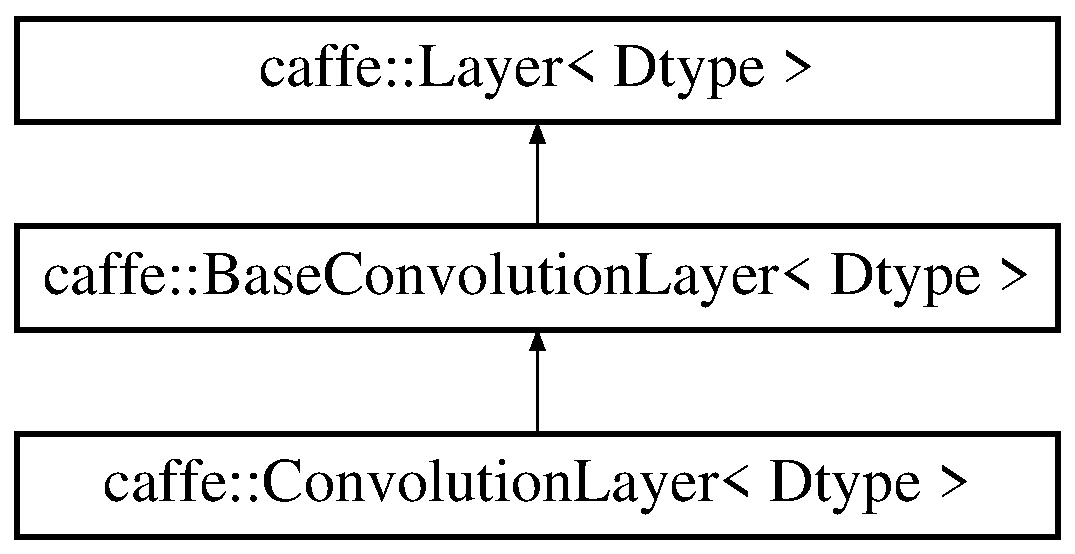
\includegraphics[height=3.000000cm]{classcaffe_1_1ConvolutionLayer}
\end{center}
\end{figure}
\subsection*{Public Member Functions}
\begin{DoxyCompactItemize}
\item 
\hyperlink{classcaffe_1_1ConvolutionLayer_ad27360afd7729001b9e4f1d8c8401866}{Convolution\+Layer} (const Layer\+Parameter \&param)
\item 
virtual const char $\ast$ \hyperlink{classcaffe_1_1ConvolutionLayer_afdcf33e7ec63ca5e476ffdc1da1f1fa0}{type} () const \hypertarget{classcaffe_1_1ConvolutionLayer_afdcf33e7ec63ca5e476ffdc1da1f1fa0}{}\label{classcaffe_1_1ConvolutionLayer_afdcf33e7ec63ca5e476ffdc1da1f1fa0}

\begin{DoxyCompactList}\small\item\em Returns the layer type. \end{DoxyCompactList}\end{DoxyCompactItemize}
\subsection*{Protected Member Functions}
\begin{DoxyCompactItemize}
\item 
virtual void \hyperlink{classcaffe_1_1ConvolutionLayer_a8505044adc26d89aae3055022898c9ea}{Forward\+\_\+cpu} (const vector$<$ \hyperlink{classcaffe_1_1Blob}{Blob}$<$ Dtype $>$ $\ast$ $>$ \&bottom, const vector$<$ \hyperlink{classcaffe_1_1Blob}{Blob}$<$ Dtype $>$ $\ast$ $>$ \&top)\hypertarget{classcaffe_1_1ConvolutionLayer_a8505044adc26d89aae3055022898c9ea}{}\label{classcaffe_1_1ConvolutionLayer_a8505044adc26d89aae3055022898c9ea}

\begin{DoxyCompactList}\small\item\em Using the C\+PU device, compute the layer output. \end{DoxyCompactList}\item 
virtual void \hyperlink{classcaffe_1_1ConvolutionLayer_ace239a41953c9207efd1a9966570825c}{Forward\+\_\+gpu} (const vector$<$ \hyperlink{classcaffe_1_1Blob}{Blob}$<$ Dtype $>$ $\ast$ $>$ \&bottom, const vector$<$ \hyperlink{classcaffe_1_1Blob}{Blob}$<$ Dtype $>$ $\ast$ $>$ \&top)\hypertarget{classcaffe_1_1ConvolutionLayer_ace239a41953c9207efd1a9966570825c}{}\label{classcaffe_1_1ConvolutionLayer_ace239a41953c9207efd1a9966570825c}

\begin{DoxyCompactList}\small\item\em Using the G\+PU device, compute the layer output. Fall back to \hyperlink{classcaffe_1_1ConvolutionLayer_a8505044adc26d89aae3055022898c9ea}{Forward\+\_\+cpu()} if unavailable. \end{DoxyCompactList}\item 
virtual void \hyperlink{classcaffe_1_1ConvolutionLayer_ac1591049f064bd88ccdc785a948ed4b2}{Backward\+\_\+cpu} (const vector$<$ \hyperlink{classcaffe_1_1Blob}{Blob}$<$ Dtype $>$ $\ast$ $>$ \&top, const vector$<$ bool $>$ \&propagate\+\_\+down, const vector$<$ \hyperlink{classcaffe_1_1Blob}{Blob}$<$ Dtype $>$ $\ast$ $>$ \&bottom)\hypertarget{classcaffe_1_1ConvolutionLayer_ac1591049f064bd88ccdc785a948ed4b2}{}\label{classcaffe_1_1ConvolutionLayer_ac1591049f064bd88ccdc785a948ed4b2}

\begin{DoxyCompactList}\small\item\em Using the C\+PU device, compute the gradients for any parameters and for the bottom blobs if propagate\+\_\+down is true. \end{DoxyCompactList}\item 
virtual void \hyperlink{classcaffe_1_1ConvolutionLayer_a4de7682afbd816037aba5da3ec66a9bb}{Backward\+\_\+gpu} (const vector$<$ \hyperlink{classcaffe_1_1Blob}{Blob}$<$ Dtype $>$ $\ast$ $>$ \&top, const vector$<$ bool $>$ \&propagate\+\_\+down, const vector$<$ \hyperlink{classcaffe_1_1Blob}{Blob}$<$ Dtype $>$ $\ast$ $>$ \&bottom)\hypertarget{classcaffe_1_1ConvolutionLayer_a4de7682afbd816037aba5da3ec66a9bb}{}\label{classcaffe_1_1ConvolutionLayer_a4de7682afbd816037aba5da3ec66a9bb}

\begin{DoxyCompactList}\small\item\em Using the G\+PU device, compute the gradients for any parameters and for the bottom blobs if propagate\+\_\+down is true. Fall back to \hyperlink{classcaffe_1_1ConvolutionLayer_ac1591049f064bd88ccdc785a948ed4b2}{Backward\+\_\+cpu()} if unavailable. \end{DoxyCompactList}\item 
virtual bool {\bfseries reverse\+\_\+dimensions} ()\hypertarget{classcaffe_1_1ConvolutionLayer_aad2f350240e3e97220230d7b4ceb9bf7}{}\label{classcaffe_1_1ConvolutionLayer_aad2f350240e3e97220230d7b4ceb9bf7}

\item 
virtual void {\bfseries compute\+\_\+output\+\_\+shape} ()\hypertarget{classcaffe_1_1ConvolutionLayer_ae6c1466c758151bf24215a06a6517cbe}{}\label{classcaffe_1_1ConvolutionLayer_ae6c1466c758151bf24215a06a6517cbe}

\end{DoxyCompactItemize}
\subsection*{Additional Inherited Members}


\subsection{Detailed Description}
\subsubsection*{template$<$typename Dtype$>$\\*
class caffe\+::\+Convolution\+Layer$<$ Dtype $>$}

Convolves the input image with a bank of learned filters, and (optionally) adds biases. 

\hyperlink{classcaffe_1_1Caffe}{Caffe} convolves by reduction to matrix multiplication. This achieves high-\/throughput and generality of input and filter dimensions but comes at the cost of memory for matrices. This makes use of efficiency in B\+L\+AS.

The input is \char`\"{}im2col\char`\"{} transformed to a channel K\textquotesingle{} x H x W data matrix for multiplication with the N x K\textquotesingle{} x H x W filter matrix to yield a N\textquotesingle{} x H x W output matrix that is then \char`\"{}col2im\char`\"{} restored. K\textquotesingle{} is the input channel $\ast$ kernel height $\ast$ kernel width dimension of the unrolled inputs so that the im2col matrix has a column for each input region to be filtered. col2im restores the output spatial structure by rolling up the output channel N\textquotesingle{} columns of the output matrix. 

\subsection{Constructor \& Destructor Documentation}
\index{caffe\+::\+Convolution\+Layer@{caffe\+::\+Convolution\+Layer}!Convolution\+Layer@{Convolution\+Layer}}
\index{Convolution\+Layer@{Convolution\+Layer}!caffe\+::\+Convolution\+Layer@{caffe\+::\+Convolution\+Layer}}
\subsubsection[{\texorpdfstring{Convolution\+Layer(const Layer\+Parameter \&param)}{ConvolutionLayer(const LayerParameter &param)}}]{\setlength{\rightskip}{0pt plus 5cm}template$<$typename Dtype $>$ {\bf caffe\+::\+Convolution\+Layer}$<$ Dtype $>$\+::{\bf Convolution\+Layer} (
\begin{DoxyParamCaption}
\item[{const Layer\+Parameter \&}]{param}
\end{DoxyParamCaption}
)\hspace{0.3cm}{\ttfamily [inline]}, {\ttfamily [explicit]}}\hypertarget{classcaffe_1_1ConvolutionLayer_ad27360afd7729001b9e4f1d8c8401866}{}\label{classcaffe_1_1ConvolutionLayer_ad27360afd7729001b9e4f1d8c8401866}

\begin{DoxyParams}{Parameters}
{\em param} & provides Convolution\+Parameter convolution\+\_\+param, with \hyperlink{classcaffe_1_1ConvolutionLayer}{Convolution\+Layer} options\+:
\begin{DoxyItemize}
\item num\+\_\+output. The number of filters.
\item kernel\+\_\+size / kernel\+\_\+h / kernel\+\_\+w. The filter dimensions, given by kernel\+\_\+size for square filters or kernel\+\_\+h and kernel\+\_\+w for rectangular filters.
\item stride / stride\+\_\+h / stride\+\_\+w ({\bfseries optional}, default 1). The filter stride, given by stride\+\_\+size for equal dimensions or stride\+\_\+h and stride\+\_\+w for different strides. By default the convolution is dense with stride 1.
\item pad / pad\+\_\+h / pad\+\_\+w ({\bfseries optional}, default 0). The zero-\/padding for convolution, given by pad for equal dimensions or pad\+\_\+h and pad\+\_\+w for different padding. Input padding is computed implicitly instead of actually padding.
\item dilation ({\bfseries optional}, default 1). The filter dilation, given by dilation\+\_\+size for equal dimensions for different dilation. By default the convolution has dilation 1.
\item group ({\bfseries optional}, default 1). The number of filter groups. Group convolution is a method for reducing parameterization by selectively connecting input and output channels. The input and output channel dimensions must be divisible by the number of groups. For group $ \geq 1 $, the convolutional filters\textquotesingle{} input and output channels are separated s.\+t. each group takes 1 / group of the input channels and makes 1 / group of the output channels. Concretely 4 input channels, 8 output channels, and 2 groups separate input channels 1-\/2 and output channels 1-\/4 into the first group and input channels 3-\/4 and output channels 5-\/8 into the second group.
\item bias\+\_\+term ({\bfseries optional}, default true). Whether to have a bias.
\item engine\+: convolution has C\+A\+F\+FE (matrix multiplication) and C\+U\+D\+NN (library kernels + stream parallelism) engines. 
\end{DoxyItemize}\\
\hline
\end{DoxyParams}


The documentation for this class was generated from the following files\+:\begin{DoxyCompactItemize}
\item 
include/caffe/layers/conv\+\_\+layer.\+hpp\item 
src/caffe/layers/conv\+\_\+layer.\+cpp\end{DoxyCompactItemize}

\hypertarget{classcaffe_1_1CPUTimer}{}\section{caffe\+:\+:C\+P\+U\+Timer Class Reference}
\label{classcaffe_1_1CPUTimer}\index{caffe\+::\+C\+P\+U\+Timer@{caffe\+::\+C\+P\+U\+Timer}}
Inheritance diagram for caffe\+:\+:C\+P\+U\+Timer\+:\begin{figure}[H]
\begin{center}
\leavevmode
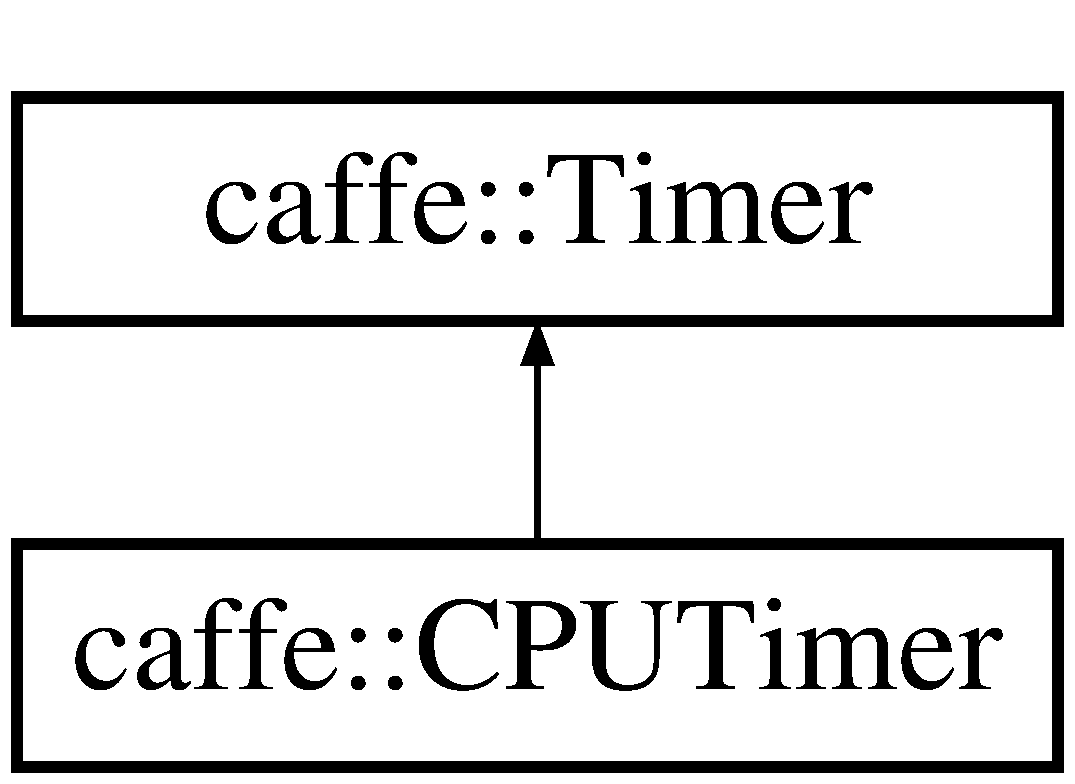
\includegraphics[height=2.000000cm]{classcaffe_1_1CPUTimer}
\end{center}
\end{figure}
\subsection*{Public Member Functions}
\begin{DoxyCompactItemize}
\item 
virtual void {\bfseries Start} ()\hypertarget{classcaffe_1_1CPUTimer_ad7d3835101e57b25373389d45b000233}{}\label{classcaffe_1_1CPUTimer_ad7d3835101e57b25373389d45b000233}

\item 
virtual void {\bfseries Stop} ()\hypertarget{classcaffe_1_1CPUTimer_a44b519b603c185b0d625d229065d07b0}{}\label{classcaffe_1_1CPUTimer_a44b519b603c185b0d625d229065d07b0}

\item 
virtual float {\bfseries Milli\+Seconds} ()\hypertarget{classcaffe_1_1CPUTimer_a08572d87bd635c3e7bdeee2b264640e5}{}\label{classcaffe_1_1CPUTimer_a08572d87bd635c3e7bdeee2b264640e5}

\item 
virtual float {\bfseries Micro\+Seconds} ()\hypertarget{classcaffe_1_1CPUTimer_a1830b20c7d04afaf8cbbd3569b54c3ee}{}\label{classcaffe_1_1CPUTimer_a1830b20c7d04afaf8cbbd3569b54c3ee}

\end{DoxyCompactItemize}
\subsection*{Additional Inherited Members}


The documentation for this class was generated from the following files\+:\begin{DoxyCompactItemize}
\item 
include/caffe/util/benchmark.\+hpp\item 
src/caffe/util/benchmark.\+cpp\end{DoxyCompactItemize}

\hypertarget{classcaffe_1_1CropLayer}{}\section{caffe\+:\+:Crop\+Layer$<$ Dtype $>$ Class Template Reference}
\label{classcaffe_1_1CropLayer}\index{caffe\+::\+Crop\+Layer$<$ Dtype $>$@{caffe\+::\+Crop\+Layer$<$ Dtype $>$}}


Takes a \hyperlink{classcaffe_1_1Blob}{Blob} and crop it, to the shape specified by the second input \hyperlink{classcaffe_1_1Blob}{Blob}, across all dimensions after the specified axis.  




{\ttfamily \#include $<$crop\+\_\+layer.\+hpp$>$}

Inheritance diagram for caffe\+:\+:Crop\+Layer$<$ Dtype $>$\+:\begin{figure}[H]
\begin{center}
\leavevmode
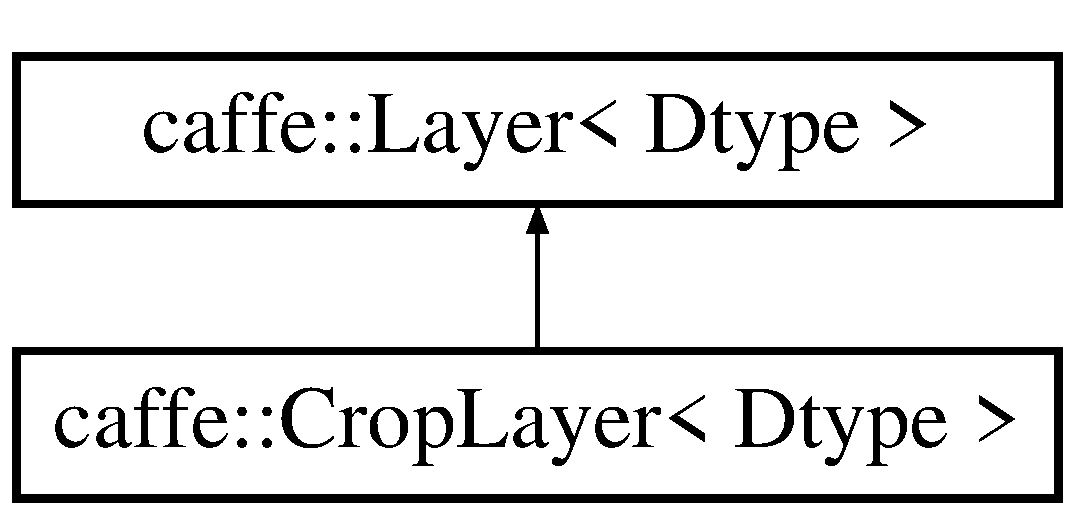
\includegraphics[height=2.000000cm]{classcaffe_1_1CropLayer}
\end{center}
\end{figure}
\subsection*{Public Member Functions}
\begin{DoxyCompactItemize}
\item 
{\bfseries Crop\+Layer} (const Layer\+Parameter \&param)\hypertarget{classcaffe_1_1CropLayer_a4baa861ad4fc049250b41111cb9588c2}{}\label{classcaffe_1_1CropLayer_a4baa861ad4fc049250b41111cb9588c2}

\item 
virtual void \hyperlink{classcaffe_1_1CropLayer_a977681a1a0b51be5bde2514542d8327c}{Layer\+Set\+Up} (const vector$<$ \hyperlink{classcaffe_1_1Blob}{Blob}$<$ Dtype $>$ $\ast$ $>$ \&bottom, const vector$<$ \hyperlink{classcaffe_1_1Blob}{Blob}$<$ Dtype $>$ $\ast$ $>$ \&top)
\begin{DoxyCompactList}\small\item\em Does layer-\/specific setup\+: your layer should implement this function as well as Reshape. \end{DoxyCompactList}\item 
virtual void \hyperlink{classcaffe_1_1CropLayer_a552d5c9829315e2fc3343b2f4965b1c8}{Reshape} (const vector$<$ \hyperlink{classcaffe_1_1Blob}{Blob}$<$ Dtype $>$ $\ast$ $>$ \&bottom, const vector$<$ \hyperlink{classcaffe_1_1Blob}{Blob}$<$ Dtype $>$ $\ast$ $>$ \&top)
\begin{DoxyCompactList}\small\item\em Adjust the shapes of top blobs and internal buffers to accommodate the shapes of the bottom blobs. \end{DoxyCompactList}\item 
virtual const char $\ast$ \hyperlink{classcaffe_1_1CropLayer_a1905800ea2ab1014ce9b67a82358cfdc}{type} () const \hypertarget{classcaffe_1_1CropLayer_a1905800ea2ab1014ce9b67a82358cfdc}{}\label{classcaffe_1_1CropLayer_a1905800ea2ab1014ce9b67a82358cfdc}

\begin{DoxyCompactList}\small\item\em Returns the layer type. \end{DoxyCompactList}\item 
virtual int \hyperlink{classcaffe_1_1CropLayer_a1c74edc80c22d805a96b00fefceb3286}{Exact\+Num\+Bottom\+Blobs} () const 
\begin{DoxyCompactList}\small\item\em Returns the exact number of bottom blobs required by the layer, or -\/1 if no exact number is required. \end{DoxyCompactList}\item 
virtual int \hyperlink{classcaffe_1_1CropLayer_a3335d668f97fe9582e29a684922adc97}{Exact\+Num\+Top\+Blobs} () const 
\begin{DoxyCompactList}\small\item\em Returns the exact number of top blobs required by the layer, or -\/1 if no exact number is required. \end{DoxyCompactList}\end{DoxyCompactItemize}
\subsection*{Protected Member Functions}
\begin{DoxyCompactItemize}
\item 
virtual void \hyperlink{classcaffe_1_1CropLayer_ac04c0c520795b4879018755d26acf7aa}{Forward\+\_\+cpu} (const vector$<$ \hyperlink{classcaffe_1_1Blob}{Blob}$<$ Dtype $>$ $\ast$ $>$ \&bottom, const vector$<$ \hyperlink{classcaffe_1_1Blob}{Blob}$<$ Dtype $>$ $\ast$ $>$ \&top)\hypertarget{classcaffe_1_1CropLayer_ac04c0c520795b4879018755d26acf7aa}{}\label{classcaffe_1_1CropLayer_ac04c0c520795b4879018755d26acf7aa}

\begin{DoxyCompactList}\small\item\em Using the C\+PU device, compute the layer output. \end{DoxyCompactList}\item 
virtual void \hyperlink{classcaffe_1_1CropLayer_abf342bcb5e278303fd0c8e90016c2df2}{Backward\+\_\+cpu} (const vector$<$ \hyperlink{classcaffe_1_1Blob}{Blob}$<$ Dtype $>$ $\ast$ $>$ \&top, const vector$<$ bool $>$ \&propagate\+\_\+down, const vector$<$ \hyperlink{classcaffe_1_1Blob}{Blob}$<$ Dtype $>$ $\ast$ $>$ \&bottom)\hypertarget{classcaffe_1_1CropLayer_abf342bcb5e278303fd0c8e90016c2df2}{}\label{classcaffe_1_1CropLayer_abf342bcb5e278303fd0c8e90016c2df2}

\begin{DoxyCompactList}\small\item\em Using the C\+PU device, compute the gradients for any parameters and for the bottom blobs if propagate\+\_\+down is true. \end{DoxyCompactList}\item 
virtual void \hyperlink{classcaffe_1_1CropLayer_a6eff85d2be46fa1701a17a26c1e54dfb}{Forward\+\_\+gpu} (const vector$<$ \hyperlink{classcaffe_1_1Blob}{Blob}$<$ Dtype $>$ $\ast$ $>$ \&bottom, const vector$<$ \hyperlink{classcaffe_1_1Blob}{Blob}$<$ Dtype $>$ $\ast$ $>$ \&top)\hypertarget{classcaffe_1_1CropLayer_a6eff85d2be46fa1701a17a26c1e54dfb}{}\label{classcaffe_1_1CropLayer_a6eff85d2be46fa1701a17a26c1e54dfb}

\begin{DoxyCompactList}\small\item\em Using the G\+PU device, compute the layer output. Fall back to \hyperlink{classcaffe_1_1CropLayer_ac04c0c520795b4879018755d26acf7aa}{Forward\+\_\+cpu()} if unavailable. \end{DoxyCompactList}\item 
virtual void \hyperlink{classcaffe_1_1CropLayer_a3a7f52f728093a219e2784d9c15be41d}{Backward\+\_\+gpu} (const vector$<$ \hyperlink{classcaffe_1_1Blob}{Blob}$<$ Dtype $>$ $\ast$ $>$ \&top, const vector$<$ bool $>$ \&propagate\+\_\+down, const vector$<$ \hyperlink{classcaffe_1_1Blob}{Blob}$<$ Dtype $>$ $\ast$ $>$ \&bottom)\hypertarget{classcaffe_1_1CropLayer_a3a7f52f728093a219e2784d9c15be41d}{}\label{classcaffe_1_1CropLayer_a3a7f52f728093a219e2784d9c15be41d}

\begin{DoxyCompactList}\small\item\em Using the G\+PU device, compute the gradients for any parameters and for the bottom blobs if propagate\+\_\+down is true. Fall back to \hyperlink{classcaffe_1_1CropLayer_abf342bcb5e278303fd0c8e90016c2df2}{Backward\+\_\+cpu()} if unavailable. \end{DoxyCompactList}\end{DoxyCompactItemize}
\subsection*{Protected Attributes}
\begin{DoxyCompactItemize}
\item 
\hyperlink{classcaffe_1_1Blob}{Blob}$<$ int $>$ {\bfseries offsets}\hypertarget{classcaffe_1_1CropLayer_a6f3f5d6bd46571c67029fb5833c633eb}{}\label{classcaffe_1_1CropLayer_a6f3f5d6bd46571c67029fb5833c633eb}

\item 
\hyperlink{classcaffe_1_1Blob}{Blob}$<$ int $>$ {\bfseries src\+\_\+strides\+\_\+}\hypertarget{classcaffe_1_1CropLayer_ad481af17ee552835c1da2d12ef555e97}{}\label{classcaffe_1_1CropLayer_ad481af17ee552835c1da2d12ef555e97}

\item 
\hyperlink{classcaffe_1_1Blob}{Blob}$<$ int $>$ {\bfseries dest\+\_\+strides\+\_\+}\hypertarget{classcaffe_1_1CropLayer_a21f818a429e142839a18b7b0693ead88}{}\label{classcaffe_1_1CropLayer_a21f818a429e142839a18b7b0693ead88}

\end{DoxyCompactItemize}


\subsection{Detailed Description}
\subsubsection*{template$<$typename Dtype$>$\\*
class caffe\+::\+Crop\+Layer$<$ Dtype $>$}

Takes a \hyperlink{classcaffe_1_1Blob}{Blob} and crop it, to the shape specified by the second input \hyperlink{classcaffe_1_1Blob}{Blob}, across all dimensions after the specified axis. 

T\+O\+D\+O(dox)\+: thorough documentation for Forward, Backward, and proto params. 

\subsection{Member Function Documentation}
\index{caffe\+::\+Crop\+Layer@{caffe\+::\+Crop\+Layer}!Exact\+Num\+Bottom\+Blobs@{Exact\+Num\+Bottom\+Blobs}}
\index{Exact\+Num\+Bottom\+Blobs@{Exact\+Num\+Bottom\+Blobs}!caffe\+::\+Crop\+Layer@{caffe\+::\+Crop\+Layer}}
\subsubsection[{\texorpdfstring{Exact\+Num\+Bottom\+Blobs() const }{ExactNumBottomBlobs() const }}]{\setlength{\rightskip}{0pt plus 5cm}template$<$typename Dtype $>$ virtual int {\bf caffe\+::\+Crop\+Layer}$<$ Dtype $>$\+::Exact\+Num\+Bottom\+Blobs (
\begin{DoxyParamCaption}
{}
\end{DoxyParamCaption}
) const\hspace{0.3cm}{\ttfamily [inline]}, {\ttfamily [virtual]}}\hypertarget{classcaffe_1_1CropLayer_a1c74edc80c22d805a96b00fefceb3286}{}\label{classcaffe_1_1CropLayer_a1c74edc80c22d805a96b00fefceb3286}


Returns the exact number of bottom blobs required by the layer, or -\/1 if no exact number is required. 

This method should be overridden to return a non-\/negative value if your layer expects some exact number of bottom blobs. 

Reimplemented from \hyperlink{classcaffe_1_1Layer_a45c7a7943a8a6735ac433c9be11e0240}{caffe\+::\+Layer$<$ Dtype $>$}.

\index{caffe\+::\+Crop\+Layer@{caffe\+::\+Crop\+Layer}!Exact\+Num\+Top\+Blobs@{Exact\+Num\+Top\+Blobs}}
\index{Exact\+Num\+Top\+Blobs@{Exact\+Num\+Top\+Blobs}!caffe\+::\+Crop\+Layer@{caffe\+::\+Crop\+Layer}}
\subsubsection[{\texorpdfstring{Exact\+Num\+Top\+Blobs() const }{ExactNumTopBlobs() const }}]{\setlength{\rightskip}{0pt plus 5cm}template$<$typename Dtype $>$ virtual int {\bf caffe\+::\+Crop\+Layer}$<$ Dtype $>$\+::Exact\+Num\+Top\+Blobs (
\begin{DoxyParamCaption}
{}
\end{DoxyParamCaption}
) const\hspace{0.3cm}{\ttfamily [inline]}, {\ttfamily [virtual]}}\hypertarget{classcaffe_1_1CropLayer_a3335d668f97fe9582e29a684922adc97}{}\label{classcaffe_1_1CropLayer_a3335d668f97fe9582e29a684922adc97}


Returns the exact number of top blobs required by the layer, or -\/1 if no exact number is required. 

This method should be overridden to return a non-\/negative value if your layer expects some exact number of top blobs. 

Reimplemented from \hyperlink{classcaffe_1_1Layer_aa3c99ed707e8db683a3043412e151af8}{caffe\+::\+Layer$<$ Dtype $>$}.

\index{caffe\+::\+Crop\+Layer@{caffe\+::\+Crop\+Layer}!Layer\+Set\+Up@{Layer\+Set\+Up}}
\index{Layer\+Set\+Up@{Layer\+Set\+Up}!caffe\+::\+Crop\+Layer@{caffe\+::\+Crop\+Layer}}
\subsubsection[{\texorpdfstring{Layer\+Set\+Up(const vector$<$ Blob$<$ Dtype $>$ $\ast$ $>$ \&bottom, const vector$<$ Blob$<$ Dtype $>$ $\ast$ $>$ \&top)}{LayerSetUp(const vector< Blob< Dtype > * > &bottom, const vector< Blob< Dtype > * > &top)}}]{\setlength{\rightskip}{0pt plus 5cm}template$<$typename Dtype $>$ void {\bf caffe\+::\+Crop\+Layer}$<$ Dtype $>$\+::Layer\+Set\+Up (
\begin{DoxyParamCaption}
\item[{const vector$<$ {\bf Blob}$<$ Dtype $>$ $\ast$ $>$ \&}]{bottom, }
\item[{const vector$<$ {\bf Blob}$<$ Dtype $>$ $\ast$ $>$ \&}]{top}
\end{DoxyParamCaption}
)\hspace{0.3cm}{\ttfamily [virtual]}}\hypertarget{classcaffe_1_1CropLayer_a977681a1a0b51be5bde2514542d8327c}{}\label{classcaffe_1_1CropLayer_a977681a1a0b51be5bde2514542d8327c}


Does layer-\/specific setup\+: your layer should implement this function as well as Reshape. 


\begin{DoxyParams}{Parameters}
{\em bottom} & the preshaped input blobs, whose data fields store the input data for this layer \\
\hline
{\em top} & the allocated but unshaped output blobs\\
\hline
\end{DoxyParams}
This method should do one-\/time layer specific setup. This includes reading and processing relevent parameters from the {\ttfamily layer\+\_\+param\+\_\+}. Setting up the shapes of top blobs and internal buffers should be done in {\ttfamily Reshape}, which will be called before the forward pass to adjust the top blob sizes. 

Reimplemented from \hyperlink{classcaffe_1_1Layer_a38dc2488bf319b8de5a7ac84e0045393}{caffe\+::\+Layer$<$ Dtype $>$}.

\index{caffe\+::\+Crop\+Layer@{caffe\+::\+Crop\+Layer}!Reshape@{Reshape}}
\index{Reshape@{Reshape}!caffe\+::\+Crop\+Layer@{caffe\+::\+Crop\+Layer}}
\subsubsection[{\texorpdfstring{Reshape(const vector$<$ Blob$<$ Dtype $>$ $\ast$ $>$ \&bottom, const vector$<$ Blob$<$ Dtype $>$ $\ast$ $>$ \&top)}{Reshape(const vector< Blob< Dtype > * > &bottom, const vector< Blob< Dtype > * > &top)}}]{\setlength{\rightskip}{0pt plus 5cm}template$<$typename Dtype $>$ void {\bf caffe\+::\+Crop\+Layer}$<$ Dtype $>$\+::Reshape (
\begin{DoxyParamCaption}
\item[{const vector$<$ {\bf Blob}$<$ Dtype $>$ $\ast$ $>$ \&}]{bottom, }
\item[{const vector$<$ {\bf Blob}$<$ Dtype $>$ $\ast$ $>$ \&}]{top}
\end{DoxyParamCaption}
)\hspace{0.3cm}{\ttfamily [virtual]}}\hypertarget{classcaffe_1_1CropLayer_a552d5c9829315e2fc3343b2f4965b1c8}{}\label{classcaffe_1_1CropLayer_a552d5c9829315e2fc3343b2f4965b1c8}


Adjust the shapes of top blobs and internal buffers to accommodate the shapes of the bottom blobs. 


\begin{DoxyParams}{Parameters}
{\em bottom} & the input blobs, with the requested input shapes \\
\hline
{\em top} & the top blobs, which should be reshaped as needed\\
\hline
\end{DoxyParams}
This method should reshape top blobs as needed according to the shapes of the bottom (input) blobs, as well as reshaping any internal buffers and making any other necessary adjustments so that the layer can accommodate the bottom blobs. 

Implements \hyperlink{classcaffe_1_1Layer_ad9d391b972c769c0ebee34ca6d1c973e}{caffe\+::\+Layer$<$ Dtype $>$}.



The documentation for this class was generated from the following files\+:\begin{DoxyCompactItemize}
\item 
include/caffe/layers/crop\+\_\+layer.\+hpp\item 
src/caffe/layers/crop\+\_\+layer.\+cpp\end{DoxyCompactItemize}

\hypertarget{classcaffe_1_1db_1_1Cursor}{}\section{caffe\+:\+:db\+:\+:Cursor Class Reference}
\label{classcaffe_1_1db_1_1Cursor}\index{caffe\+::db\+::\+Cursor@{caffe\+::db\+::\+Cursor}}
\subsection*{Public Member Functions}
\begin{DoxyCompactItemize}
\item 
virtual void {\bfseries Seek\+To\+First} ()=0\hypertarget{classcaffe_1_1db_1_1Cursor_a07896b619ea1e802b8d3b55782ef3a8a}{}\label{classcaffe_1_1db_1_1Cursor_a07896b619ea1e802b8d3b55782ef3a8a}

\item 
virtual void {\bfseries Next} ()=0\hypertarget{classcaffe_1_1db_1_1Cursor_ab90dc953417f37d0d4247b125ea1ae37}{}\label{classcaffe_1_1db_1_1Cursor_ab90dc953417f37d0d4247b125ea1ae37}

\item 
virtual string {\bfseries key} ()=0\hypertarget{classcaffe_1_1db_1_1Cursor_a87ec068564018e9218360db6fb1dade3}{}\label{classcaffe_1_1db_1_1Cursor_a87ec068564018e9218360db6fb1dade3}

\item 
virtual string {\bfseries value} ()=0\hypertarget{classcaffe_1_1db_1_1Cursor_ad6de2be246e7b46c00d34c29b24e16ee}{}\label{classcaffe_1_1db_1_1Cursor_ad6de2be246e7b46c00d34c29b24e16ee}

\item 
virtual bool {\bfseries valid} ()=0\hypertarget{classcaffe_1_1db_1_1Cursor_ae3811414ce9044a639195462be9e4f38}{}\label{classcaffe_1_1db_1_1Cursor_ae3811414ce9044a639195462be9e4f38}

\item 
{\bfseries D\+I\+S\+A\+B\+L\+E\+\_\+\+C\+O\+P\+Y\+\_\+\+A\+N\+D\+\_\+\+A\+S\+S\+I\+GN} (\hyperlink{classcaffe_1_1db_1_1Cursor}{Cursor})\hypertarget{classcaffe_1_1db_1_1Cursor_acbd3ccf06a180bd19079a2fec0a6a8f2}{}\label{classcaffe_1_1db_1_1Cursor_acbd3ccf06a180bd19079a2fec0a6a8f2}

\end{DoxyCompactItemize}


The documentation for this class was generated from the following file\+:\begin{DoxyCompactItemize}
\item 
include/caffe/util/db.\+hpp\end{DoxyCompactItemize}

\hypertarget{classcaffe_1_1DataLayer}{}\section{caffe\+:\+:Data\+Layer$<$ Dtype $>$ Class Template Reference}
\label{classcaffe_1_1DataLayer}\index{caffe\+::\+Data\+Layer$<$ Dtype $>$@{caffe\+::\+Data\+Layer$<$ Dtype $>$}}
Inheritance diagram for caffe\+:\+:Data\+Layer$<$ Dtype $>$\+:\begin{figure}[H]
\begin{center}
\leavevmode
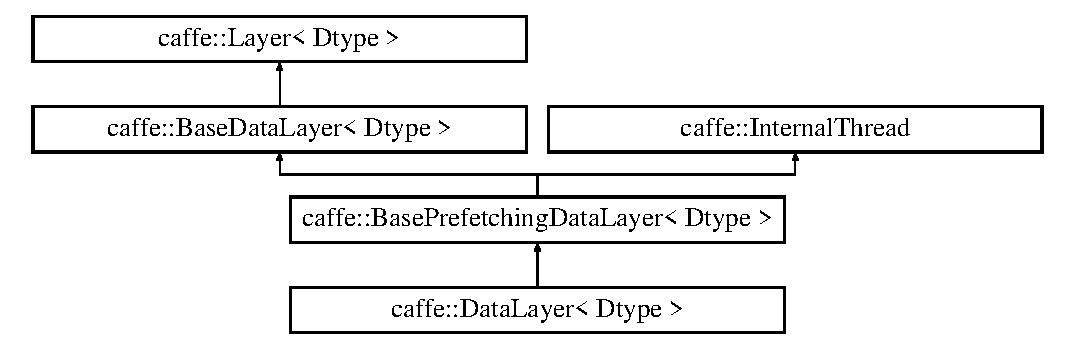
\includegraphics[height=4.000000cm]{classcaffe_1_1DataLayer}
\end{center}
\end{figure}
\subsection*{Public Member Functions}
\begin{DoxyCompactItemize}
\item 
{\bfseries Data\+Layer} (const Layer\+Parameter \&param)\hypertarget{classcaffe_1_1DataLayer_a55d92ba6737e695551eca610868f1fae}{}\label{classcaffe_1_1DataLayer_a55d92ba6737e695551eca610868f1fae}

\item 
virtual void {\bfseries Data\+Layer\+Set\+Up} (const vector$<$ \hyperlink{classcaffe_1_1Blob}{Blob}$<$ Dtype $>$ $\ast$ $>$ \&bottom, const vector$<$ \hyperlink{classcaffe_1_1Blob}{Blob}$<$ Dtype $>$ $\ast$ $>$ \&top)\hypertarget{classcaffe_1_1DataLayer_a7c9ee1ab0a5be8030f03a5700ce42de4}{}\label{classcaffe_1_1DataLayer_a7c9ee1ab0a5be8030f03a5700ce42de4}

\item 
virtual const char $\ast$ \hyperlink{classcaffe_1_1DataLayer_a8a7454b2fc8bde3220c21b8918c9ac2a}{type} () const \hypertarget{classcaffe_1_1DataLayer_a8a7454b2fc8bde3220c21b8918c9ac2a}{}\label{classcaffe_1_1DataLayer_a8a7454b2fc8bde3220c21b8918c9ac2a}

\begin{DoxyCompactList}\small\item\em Returns the layer type. \end{DoxyCompactList}\item 
virtual int \hyperlink{classcaffe_1_1DataLayer_a41c3c270f2f1239808fbd4293e89949d}{Exact\+Num\+Bottom\+Blobs} () const 
\begin{DoxyCompactList}\small\item\em Returns the exact number of bottom blobs required by the layer, or -\/1 if no exact number is required. \end{DoxyCompactList}\item 
virtual int \hyperlink{classcaffe_1_1DataLayer_a65a81d2aff2703bf94b630ba2657b319}{Min\+Top\+Blobs} () const 
\begin{DoxyCompactList}\small\item\em Returns the minimum number of top blobs required by the layer, or -\/1 if no minimum number is required. \end{DoxyCompactList}\item 
virtual int \hyperlink{classcaffe_1_1DataLayer_a67d8d7543045833765d73c850a81941f}{Max\+Top\+Blobs} () const 
\begin{DoxyCompactList}\small\item\em Returns the maximum number of top blobs required by the layer, or -\/1 if no maximum number is required. \end{DoxyCompactList}\end{DoxyCompactItemize}
\subsection*{Protected Member Functions}
\begin{DoxyCompactItemize}
\item 
void {\bfseries Next} ()\hypertarget{classcaffe_1_1DataLayer_a16238c3e219f4215faa4da08f670551f}{}\label{classcaffe_1_1DataLayer_a16238c3e219f4215faa4da08f670551f}

\item 
bool {\bfseries Skip} ()\hypertarget{classcaffe_1_1DataLayer_a230e84eafe73df8e7da3c41b2e3430e1}{}\label{classcaffe_1_1DataLayer_a230e84eafe73df8e7da3c41b2e3430e1}

\item 
virtual void {\bfseries load\+\_\+batch} (\hyperlink{classcaffe_1_1Batch}{Batch}$<$ Dtype $>$ $\ast$batch)\hypertarget{classcaffe_1_1DataLayer_a5f14e385399a658476642d225a2827f9}{}\label{classcaffe_1_1DataLayer_a5f14e385399a658476642d225a2827f9}

\end{DoxyCompactItemize}
\subsection*{Protected Attributes}
\begin{DoxyCompactItemize}
\item 
shared\+\_\+ptr$<$ \hyperlink{classcaffe_1_1db_1_1DB}{db\+::\+DB} $>$ {\bfseries db\+\_\+}\hypertarget{classcaffe_1_1DataLayer_af6384a1dcc37d32c7f556080da3c006d}{}\label{classcaffe_1_1DataLayer_af6384a1dcc37d32c7f556080da3c006d}

\item 
shared\+\_\+ptr$<$ \hyperlink{classcaffe_1_1db_1_1Cursor}{db\+::\+Cursor} $>$ {\bfseries cursor\+\_\+}\hypertarget{classcaffe_1_1DataLayer_ad26510baf81f48d92569ea95a8643af0}{}\label{classcaffe_1_1DataLayer_ad26510baf81f48d92569ea95a8643af0}

\item 
uint64\+\_\+t {\bfseries offset\+\_\+}\hypertarget{classcaffe_1_1DataLayer_a1af404785922d764270d7d5a195d90df}{}\label{classcaffe_1_1DataLayer_a1af404785922d764270d7d5a195d90df}

\end{DoxyCompactItemize}


\subsection{Member Function Documentation}
\index{caffe\+::\+Data\+Layer@{caffe\+::\+Data\+Layer}!Exact\+Num\+Bottom\+Blobs@{Exact\+Num\+Bottom\+Blobs}}
\index{Exact\+Num\+Bottom\+Blobs@{Exact\+Num\+Bottom\+Blobs}!caffe\+::\+Data\+Layer@{caffe\+::\+Data\+Layer}}
\subsubsection[{\texorpdfstring{Exact\+Num\+Bottom\+Blobs() const }{ExactNumBottomBlobs() const }}]{\setlength{\rightskip}{0pt plus 5cm}template$<$typename Dtype $>$ virtual int {\bf caffe\+::\+Data\+Layer}$<$ Dtype $>$\+::Exact\+Num\+Bottom\+Blobs (
\begin{DoxyParamCaption}
{}
\end{DoxyParamCaption}
) const\hspace{0.3cm}{\ttfamily [inline]}, {\ttfamily [virtual]}}\hypertarget{classcaffe_1_1DataLayer_a41c3c270f2f1239808fbd4293e89949d}{}\label{classcaffe_1_1DataLayer_a41c3c270f2f1239808fbd4293e89949d}


Returns the exact number of bottom blobs required by the layer, or -\/1 if no exact number is required. 

This method should be overridden to return a non-\/negative value if your layer expects some exact number of bottom blobs. 

Reimplemented from \hyperlink{classcaffe_1_1Layer_a45c7a7943a8a6735ac433c9be11e0240}{caffe\+::\+Layer$<$ Dtype $>$}.

\index{caffe\+::\+Data\+Layer@{caffe\+::\+Data\+Layer}!Max\+Top\+Blobs@{Max\+Top\+Blobs}}
\index{Max\+Top\+Blobs@{Max\+Top\+Blobs}!caffe\+::\+Data\+Layer@{caffe\+::\+Data\+Layer}}
\subsubsection[{\texorpdfstring{Max\+Top\+Blobs() const }{MaxTopBlobs() const }}]{\setlength{\rightskip}{0pt plus 5cm}template$<$typename Dtype $>$ virtual int {\bf caffe\+::\+Data\+Layer}$<$ Dtype $>$\+::Max\+Top\+Blobs (
\begin{DoxyParamCaption}
{}
\end{DoxyParamCaption}
) const\hspace{0.3cm}{\ttfamily [inline]}, {\ttfamily [virtual]}}\hypertarget{classcaffe_1_1DataLayer_a67d8d7543045833765d73c850a81941f}{}\label{classcaffe_1_1DataLayer_a67d8d7543045833765d73c850a81941f}


Returns the maximum number of top blobs required by the layer, or -\/1 if no maximum number is required. 

This method should be overridden to return a non-\/negative value if your layer expects some maximum number of top blobs. 

Reimplemented from \hyperlink{classcaffe_1_1Layer_adeff774663c6ec94424901d2746e2f03}{caffe\+::\+Layer$<$ Dtype $>$}.

\index{caffe\+::\+Data\+Layer@{caffe\+::\+Data\+Layer}!Min\+Top\+Blobs@{Min\+Top\+Blobs}}
\index{Min\+Top\+Blobs@{Min\+Top\+Blobs}!caffe\+::\+Data\+Layer@{caffe\+::\+Data\+Layer}}
\subsubsection[{\texorpdfstring{Min\+Top\+Blobs() const }{MinTopBlobs() const }}]{\setlength{\rightskip}{0pt plus 5cm}template$<$typename Dtype $>$ virtual int {\bf caffe\+::\+Data\+Layer}$<$ Dtype $>$\+::Min\+Top\+Blobs (
\begin{DoxyParamCaption}
{}
\end{DoxyParamCaption}
) const\hspace{0.3cm}{\ttfamily [inline]}, {\ttfamily [virtual]}}\hypertarget{classcaffe_1_1DataLayer_a65a81d2aff2703bf94b630ba2657b319}{}\label{classcaffe_1_1DataLayer_a65a81d2aff2703bf94b630ba2657b319}


Returns the minimum number of top blobs required by the layer, or -\/1 if no minimum number is required. 

This method should be overridden to return a non-\/negative value if your layer expects some minimum number of top blobs. 

Reimplemented from \hyperlink{classcaffe_1_1Layer_a8bb143d58a740345fa2dc3d4204d553b}{caffe\+::\+Layer$<$ Dtype $>$}.



The documentation for this class was generated from the following files\+:\begin{DoxyCompactItemize}
\item 
include/caffe/layers/data\+\_\+layer.\+hpp\item 
src/caffe/layers/data\+\_\+layer.\+cpp\end{DoxyCompactItemize}

\hypertarget{classcaffe_1_1DataTransformer}{}\section{caffe\+:\+:Data\+Transformer$<$ Dtype $>$ Class Template Reference}
\label{classcaffe_1_1DataTransformer}\index{caffe\+::\+Data\+Transformer$<$ Dtype $>$@{caffe\+::\+Data\+Transformer$<$ Dtype $>$}}


Applies common transformations to the input data, such as scaling, mirroring, substracting the image mean...  




{\ttfamily \#include $<$data\+\_\+transformer.\+hpp$>$}

\subsection*{Public Member Functions}
\begin{DoxyCompactItemize}
\item 
{\bfseries Data\+Transformer} (const Transformation\+Parameter \&param, Phase phase)\hypertarget{classcaffe_1_1DataTransformer_ae598f617042b2d68f4bab0dd3bd542f0}{}\label{classcaffe_1_1DataTransformer_ae598f617042b2d68f4bab0dd3bd542f0}

\item 
void \hyperlink{classcaffe_1_1DataTransformer_a6d807c7dc250e66b62d97d9847278e68}{Init\+Rand} ()\hypertarget{classcaffe_1_1DataTransformer_a6d807c7dc250e66b62d97d9847278e68}{}\label{classcaffe_1_1DataTransformer_a6d807c7dc250e66b62d97d9847278e68}

\begin{DoxyCompactList}\small\item\em Initialize the Random number generations if needed by the transformation. \end{DoxyCompactList}\item 
void \hyperlink{classcaffe_1_1DataTransformer_a1626db49587d506a91e7b70373ace816}{Transform} (const Datum \&datum, \hyperlink{classcaffe_1_1Blob}{Blob}$<$ Dtype $>$ $\ast$transformed\+\_\+blob)
\begin{DoxyCompactList}\small\item\em Applies the transformation defined in the data layer\textquotesingle{}s transform\+\_\+param block to the data. \end{DoxyCompactList}\item 
void \hyperlink{classcaffe_1_1DataTransformer_a082cad626c5f51c9f8d93bb88cca1bd0}{Transform} (const vector$<$ Datum $>$ \&datum\+\_\+vector, \hyperlink{classcaffe_1_1Blob}{Blob}$<$ Dtype $>$ $\ast$transformed\+\_\+blob)
\begin{DoxyCompactList}\small\item\em Applies the transformation defined in the data layer\textquotesingle{}s transform\+\_\+param block to a vector of Datum. \end{DoxyCompactList}\item 
void \hyperlink{classcaffe_1_1DataTransformer_a168abf1bf9466420da6968178c6edb4d}{Transform} (\hyperlink{classcaffe_1_1Blob}{Blob}$<$ Dtype $>$ $\ast$input\+\_\+blob, \hyperlink{classcaffe_1_1Blob}{Blob}$<$ Dtype $>$ $\ast$transformed\+\_\+blob)
\begin{DoxyCompactList}\small\item\em Applies the same transformation defined in the data layer\textquotesingle{}s transform\+\_\+param block to all the num images in a input\+\_\+blob. \end{DoxyCompactList}\item 
vector$<$ int $>$ \hyperlink{classcaffe_1_1DataTransformer_a1e43b0fb80cded5bb854e1a06004bebf}{Infer\+Blob\+Shape} (const Datum \&datum)
\begin{DoxyCompactList}\small\item\em Infers the shape of transformed\+\_\+blob will have when the transformation is applied to the data. \end{DoxyCompactList}\item 
vector$<$ int $>$ \hyperlink{classcaffe_1_1DataTransformer_ac829dd6448dcce67acb1e22a2554db4b}{Infer\+Blob\+Shape} (const vector$<$ Datum $>$ \&datum\+\_\+vector)
\begin{DoxyCompactList}\small\item\em Infers the shape of transformed\+\_\+blob will have when the transformation is applied to the data. It uses the first element to infer the shape of the blob. \end{DoxyCompactList}\end{DoxyCompactItemize}
\subsection*{Protected Member Functions}
\begin{DoxyCompactItemize}
\item 
virtual int \hyperlink{classcaffe_1_1DataTransformer_ac3e52731074a73b05ff0527d2febc8f2}{Rand} (int n)
\begin{DoxyCompactList}\small\item\em Infers the shape of transformed\+\_\+blob will have when the transformation is applied to the data. It uses the first element to infer the shape of the blob. \end{DoxyCompactList}\item 
void {\bfseries Transform} (const Datum \&datum, Dtype $\ast$transformed\+\_\+data)\hypertarget{classcaffe_1_1DataTransformer_a96c70b694d85f763934274e2fd92e6eb}{}\label{classcaffe_1_1DataTransformer_a96c70b694d85f763934274e2fd92e6eb}

\end{DoxyCompactItemize}
\subsection*{Protected Attributes}
\begin{DoxyCompactItemize}
\item 
Transformation\+Parameter {\bfseries param\+\_\+}\hypertarget{classcaffe_1_1DataTransformer_a7d0dd7f13701a450c37c989a39ac50e0}{}\label{classcaffe_1_1DataTransformer_a7d0dd7f13701a450c37c989a39ac50e0}

\item 
shared\+\_\+ptr$<$ \hyperlink{classcaffe_1_1Caffe_1_1RNG}{Caffe\+::\+R\+NG} $>$ {\bfseries rng\+\_\+}\hypertarget{classcaffe_1_1DataTransformer_a28e1ac0553c09e21036f671b73a1e0dd}{}\label{classcaffe_1_1DataTransformer_a28e1ac0553c09e21036f671b73a1e0dd}

\item 
Phase {\bfseries phase\+\_\+}\hypertarget{classcaffe_1_1DataTransformer_a30cf039d7452683f4f91e022fd8eec32}{}\label{classcaffe_1_1DataTransformer_a30cf039d7452683f4f91e022fd8eec32}

\item 
\hyperlink{classcaffe_1_1Blob}{Blob}$<$ Dtype $>$ {\bfseries data\+\_\+mean\+\_\+}\hypertarget{classcaffe_1_1DataTransformer_a74d5da590321195fdaa7d2c9f6b372fd}{}\label{classcaffe_1_1DataTransformer_a74d5da590321195fdaa7d2c9f6b372fd}

\item 
vector$<$ Dtype $>$ {\bfseries mean\+\_\+values\+\_\+}\hypertarget{classcaffe_1_1DataTransformer_a04a2c85e464047c84b98aa677ad19d94}{}\label{classcaffe_1_1DataTransformer_a04a2c85e464047c84b98aa677ad19d94}

\end{DoxyCompactItemize}


\subsection{Detailed Description}
\subsubsection*{template$<$typename Dtype$>$\\*
class caffe\+::\+Data\+Transformer$<$ Dtype $>$}

Applies common transformations to the input data, such as scaling, mirroring, substracting the image mean... 

\subsection{Member Function Documentation}
\index{caffe\+::\+Data\+Transformer@{caffe\+::\+Data\+Transformer}!Infer\+Blob\+Shape@{Infer\+Blob\+Shape}}
\index{Infer\+Blob\+Shape@{Infer\+Blob\+Shape}!caffe\+::\+Data\+Transformer@{caffe\+::\+Data\+Transformer}}
\subsubsection[{\texorpdfstring{Infer\+Blob\+Shape(const Datum \&datum)}{InferBlobShape(const Datum &datum)}}]{\setlength{\rightskip}{0pt plus 5cm}template$<$typename Dtype $>$ vector$<$ int $>$ {\bf caffe\+::\+Data\+Transformer}$<$ Dtype $>$\+::Infer\+Blob\+Shape (
\begin{DoxyParamCaption}
\item[{const Datum \&}]{datum}
\end{DoxyParamCaption}
)}\hypertarget{classcaffe_1_1DataTransformer_a1e43b0fb80cded5bb854e1a06004bebf}{}\label{classcaffe_1_1DataTransformer_a1e43b0fb80cded5bb854e1a06004bebf}


Infers the shape of transformed\+\_\+blob will have when the transformation is applied to the data. 


\begin{DoxyParams}{Parameters}
{\em datum} & Datum containing the data to be transformed. \\
\hline
\end{DoxyParams}
\index{caffe\+::\+Data\+Transformer@{caffe\+::\+Data\+Transformer}!Infer\+Blob\+Shape@{Infer\+Blob\+Shape}}
\index{Infer\+Blob\+Shape@{Infer\+Blob\+Shape}!caffe\+::\+Data\+Transformer@{caffe\+::\+Data\+Transformer}}
\subsubsection[{\texorpdfstring{Infer\+Blob\+Shape(const vector$<$ Datum $>$ \&datum\+\_\+vector)}{InferBlobShape(const vector< Datum > &datum_vector)}}]{\setlength{\rightskip}{0pt plus 5cm}template$<$typename Dtype $>$ vector$<$ int $>$ {\bf caffe\+::\+Data\+Transformer}$<$ Dtype $>$\+::Infer\+Blob\+Shape (
\begin{DoxyParamCaption}
\item[{const vector$<$ Datum $>$ \&}]{datum\+\_\+vector}
\end{DoxyParamCaption}
)}\hypertarget{classcaffe_1_1DataTransformer_ac829dd6448dcce67acb1e22a2554db4b}{}\label{classcaffe_1_1DataTransformer_ac829dd6448dcce67acb1e22a2554db4b}


Infers the shape of transformed\+\_\+blob will have when the transformation is applied to the data. It uses the first element to infer the shape of the blob. 


\begin{DoxyParams}{Parameters}
{\em datum\+\_\+vector} & A vector of Datum containing the data to be transformed. \\
\hline
\end{DoxyParams}
\index{caffe\+::\+Data\+Transformer@{caffe\+::\+Data\+Transformer}!Rand@{Rand}}
\index{Rand@{Rand}!caffe\+::\+Data\+Transformer@{caffe\+::\+Data\+Transformer}}
\subsubsection[{\texorpdfstring{Rand(int n)}{Rand(int n)}}]{\setlength{\rightskip}{0pt plus 5cm}template$<$typename Dtype $>$ int {\bf caffe\+::\+Data\+Transformer}$<$ Dtype $>$\+::Rand (
\begin{DoxyParamCaption}
\item[{int}]{n}
\end{DoxyParamCaption}
)\hspace{0.3cm}{\ttfamily [protected]}, {\ttfamily [virtual]}}\hypertarget{classcaffe_1_1DataTransformer_ac3e52731074a73b05ff0527d2febc8f2}{}\label{classcaffe_1_1DataTransformer_ac3e52731074a73b05ff0527d2febc8f2}


Infers the shape of transformed\+\_\+blob will have when the transformation is applied to the data. It uses the first element to infer the shape of the blob. 


\begin{DoxyParams}{Parameters}
{\em mat\+\_\+vector} & A vector of Mat containing the data to be transformed. Generates a random integer from Uniform(\{0, 1, ..., n-\/1\}).\\
\hline
{\em n} & The upperbound (exclusive) value of the random number. \\
\hline
\end{DoxyParams}
\begin{DoxyReturn}{Returns}
A uniformly random integer value from (\{0, 1, ..., n-\/1\}). 
\end{DoxyReturn}
\index{caffe\+::\+Data\+Transformer@{caffe\+::\+Data\+Transformer}!Transform@{Transform}}
\index{Transform@{Transform}!caffe\+::\+Data\+Transformer@{caffe\+::\+Data\+Transformer}}
\subsubsection[{\texorpdfstring{Transform(const Datum \&datum, Blob$<$ Dtype $>$ $\ast$transformed\+\_\+blob)}{Transform(const Datum &datum, Blob< Dtype > *transformed_blob)}}]{\setlength{\rightskip}{0pt plus 5cm}template$<$typename Dtype $>$ void {\bf caffe\+::\+Data\+Transformer}$<$ Dtype $>$\+::Transform (
\begin{DoxyParamCaption}
\item[{const Datum \&}]{datum, }
\item[{{\bf Blob}$<$ Dtype $>$ $\ast$}]{transformed\+\_\+blob}
\end{DoxyParamCaption}
)}\hypertarget{classcaffe_1_1DataTransformer_a1626db49587d506a91e7b70373ace816}{}\label{classcaffe_1_1DataTransformer_a1626db49587d506a91e7b70373ace816}


Applies the transformation defined in the data layer\textquotesingle{}s transform\+\_\+param block to the data. 


\begin{DoxyParams}{Parameters}
{\em datum} & Datum containing the data to be transformed. \\
\hline
{\em transformed\+\_\+blob} & This is destination blob. It can be part of top blob\textquotesingle{}s data if set\+\_\+cpu\+\_\+data() is used. See data\+\_\+layer.\+cpp for an example. \\
\hline
\end{DoxyParams}
\index{caffe\+::\+Data\+Transformer@{caffe\+::\+Data\+Transformer}!Transform@{Transform}}
\index{Transform@{Transform}!caffe\+::\+Data\+Transformer@{caffe\+::\+Data\+Transformer}}
\subsubsection[{\texorpdfstring{Transform(const vector$<$ Datum $>$ \&datum\+\_\+vector, Blob$<$ Dtype $>$ $\ast$transformed\+\_\+blob)}{Transform(const vector< Datum > &datum_vector, Blob< Dtype > *transformed_blob)}}]{\setlength{\rightskip}{0pt plus 5cm}template$<$typename Dtype $>$ void {\bf caffe\+::\+Data\+Transformer}$<$ Dtype $>$\+::Transform (
\begin{DoxyParamCaption}
\item[{const vector$<$ Datum $>$ \&}]{datum\+\_\+vector, }
\item[{{\bf Blob}$<$ Dtype $>$ $\ast$}]{transformed\+\_\+blob}
\end{DoxyParamCaption}
)}\hypertarget{classcaffe_1_1DataTransformer_a082cad626c5f51c9f8d93bb88cca1bd0}{}\label{classcaffe_1_1DataTransformer_a082cad626c5f51c9f8d93bb88cca1bd0}


Applies the transformation defined in the data layer\textquotesingle{}s transform\+\_\+param block to a vector of Datum. 


\begin{DoxyParams}{Parameters}
{\em datum\+\_\+vector} & A vector of Datum containing the data to be transformed. \\
\hline
{\em transformed\+\_\+blob} & This is destination blob. It can be part of top blob\textquotesingle{}s data if set\+\_\+cpu\+\_\+data() is used. See memory\+\_\+layer.\+cpp for an example. \\
\hline
\end{DoxyParams}
\index{caffe\+::\+Data\+Transformer@{caffe\+::\+Data\+Transformer}!Transform@{Transform}}
\index{Transform@{Transform}!caffe\+::\+Data\+Transformer@{caffe\+::\+Data\+Transformer}}
\subsubsection[{\texorpdfstring{Transform(\+Blob$<$ Dtype $>$ $\ast$input\+\_\+blob, Blob$<$ Dtype $>$ $\ast$transformed\+\_\+blob)}{Transform(Blob< Dtype > *input_blob, Blob< Dtype > *transformed_blob)}}]{\setlength{\rightskip}{0pt plus 5cm}template$<$typename Dtype $>$ void {\bf caffe\+::\+Data\+Transformer}$<$ Dtype $>$\+::Transform (
\begin{DoxyParamCaption}
\item[{{\bf Blob}$<$ Dtype $>$ $\ast$}]{input\+\_\+blob, }
\item[{{\bf Blob}$<$ Dtype $>$ $\ast$}]{transformed\+\_\+blob}
\end{DoxyParamCaption}
)}\hypertarget{classcaffe_1_1DataTransformer_a168abf1bf9466420da6968178c6edb4d}{}\label{classcaffe_1_1DataTransformer_a168abf1bf9466420da6968178c6edb4d}


Applies the same transformation defined in the data layer\textquotesingle{}s transform\+\_\+param block to all the num images in a input\+\_\+blob. 


\begin{DoxyParams}{Parameters}
{\em input\+\_\+blob} & A \hyperlink{classcaffe_1_1Blob}{Blob} containing the data to be transformed. It applies the same transformation to all the num images in the blob. \\
\hline
{\em transformed\+\_\+blob} & This is destination blob, it will contain as many images as the input blob. It can be part of top blob\textquotesingle{}s data. \\
\hline
\end{DoxyParams}


The documentation for this class was generated from the following files\+:\begin{DoxyCompactItemize}
\item 
include/caffe/data\+\_\+transformer.\+hpp\item 
src/caffe/data\+\_\+transformer.\+cpp\end{DoxyCompactItemize}

\hypertarget{classcaffe_1_1db_1_1DB}{}\section{caffe\+:\+:db\+:\+:DB Class Reference}
\label{classcaffe_1_1db_1_1DB}\index{caffe\+::db\+::\+DB@{caffe\+::db\+::\+DB}}
\subsection*{Public Member Functions}
\begin{DoxyCompactItemize}
\item 
virtual void {\bfseries Open} (const string \&source, Mode mode)=0\hypertarget{classcaffe_1_1db_1_1DB_acb14bf3840539c0ce5bfd294f31adb67}{}\label{classcaffe_1_1db_1_1DB_acb14bf3840539c0ce5bfd294f31adb67}

\item 
virtual void {\bfseries Close} ()=0\hypertarget{classcaffe_1_1db_1_1DB_a1eea40ee9e2017c2aa983e88770486fc}{}\label{classcaffe_1_1db_1_1DB_a1eea40ee9e2017c2aa983e88770486fc}

\item 
virtual \hyperlink{classcaffe_1_1db_1_1Cursor}{Cursor} $\ast$ {\bfseries New\+Cursor} ()=0\hypertarget{classcaffe_1_1db_1_1DB_a5bf502b15bfb2f8fbbf1670bf1a2e93b}{}\label{classcaffe_1_1db_1_1DB_a5bf502b15bfb2f8fbbf1670bf1a2e93b}

\item 
virtual \hyperlink{classcaffe_1_1db_1_1Transaction}{Transaction} $\ast$ {\bfseries New\+Transaction} ()=0\hypertarget{classcaffe_1_1db_1_1DB_a346f1668d90dc24492ffc0d2d9f7097c}{}\label{classcaffe_1_1db_1_1DB_a346f1668d90dc24492ffc0d2d9f7097c}

\item 
{\bfseries D\+I\+S\+A\+B\+L\+E\+\_\+\+C\+O\+P\+Y\+\_\+\+A\+N\+D\+\_\+\+A\+S\+S\+I\+GN} (\hyperlink{classcaffe_1_1db_1_1DB}{DB})\hypertarget{classcaffe_1_1db_1_1DB_aaffc660573d0b233cb2dfecf2e3aabae}{}\label{classcaffe_1_1db_1_1DB_aaffc660573d0b233cb2dfecf2e3aabae}

\end{DoxyCompactItemize}


The documentation for this class was generated from the following file\+:\begin{DoxyCompactItemize}
\item 
include/caffe/util/db.\+hpp\end{DoxyCompactItemize}

\hypertarget{classcaffe_1_1DeconvolutionLayer}{}\section{caffe\+:\+:Deconvolution\+Layer$<$ Dtype $>$ Class Template Reference}
\label{classcaffe_1_1DeconvolutionLayer}\index{caffe\+::\+Deconvolution\+Layer$<$ Dtype $>$@{caffe\+::\+Deconvolution\+Layer$<$ Dtype $>$}}


Convolve the input with a bank of learned filters, and (optionally) add biases, treating filters and convolution parameters in the opposite sense as \hyperlink{classcaffe_1_1ConvolutionLayer}{Convolution\+Layer}.  




{\ttfamily \#include $<$deconv\+\_\+layer.\+hpp$>$}

Inheritance diagram for caffe\+:\+:Deconvolution\+Layer$<$ Dtype $>$\+:\begin{figure}[H]
\begin{center}
\leavevmode
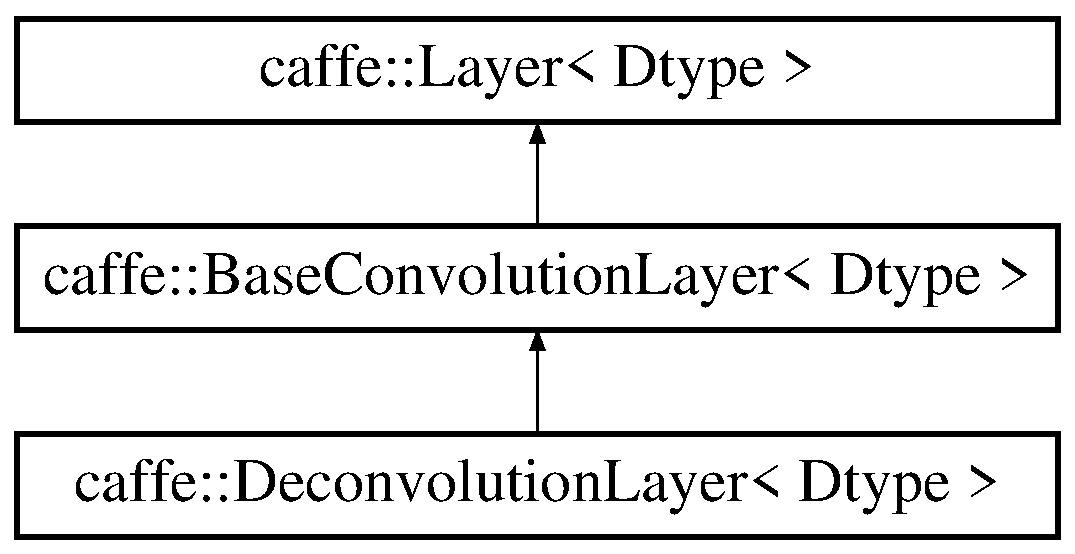
\includegraphics[height=3.000000cm]{classcaffe_1_1DeconvolutionLayer}
\end{center}
\end{figure}
\subsection*{Public Member Functions}
\begin{DoxyCompactItemize}
\item 
{\bfseries Deconvolution\+Layer} (const Layer\+Parameter \&param)\hypertarget{classcaffe_1_1DeconvolutionLayer_a48f1d8c75f9fb83d4af78a84cff187e8}{}\label{classcaffe_1_1DeconvolutionLayer_a48f1d8c75f9fb83d4af78a84cff187e8}

\item 
virtual const char $\ast$ \hyperlink{classcaffe_1_1DeconvolutionLayer_a7498a14d8b7afa0bc85abe1dbd719135}{type} () const \hypertarget{classcaffe_1_1DeconvolutionLayer_a7498a14d8b7afa0bc85abe1dbd719135}{}\label{classcaffe_1_1DeconvolutionLayer_a7498a14d8b7afa0bc85abe1dbd719135}

\begin{DoxyCompactList}\small\item\em Returns the layer type. \end{DoxyCompactList}\end{DoxyCompactItemize}
\subsection*{Protected Member Functions}
\begin{DoxyCompactItemize}
\item 
virtual void \hyperlink{classcaffe_1_1DeconvolutionLayer_a3716cda5f7d7e81f7d19cf4313d2bfc5}{Forward\+\_\+cpu} (const vector$<$ \hyperlink{classcaffe_1_1Blob}{Blob}$<$ Dtype $>$ $\ast$ $>$ \&bottom, const vector$<$ \hyperlink{classcaffe_1_1Blob}{Blob}$<$ Dtype $>$ $\ast$ $>$ \&top)\hypertarget{classcaffe_1_1DeconvolutionLayer_a3716cda5f7d7e81f7d19cf4313d2bfc5}{}\label{classcaffe_1_1DeconvolutionLayer_a3716cda5f7d7e81f7d19cf4313d2bfc5}

\begin{DoxyCompactList}\small\item\em Using the C\+PU device, compute the layer output. \end{DoxyCompactList}\item 
virtual void \hyperlink{classcaffe_1_1DeconvolutionLayer_a49c3360133291f7e6593db36ec392d07}{Forward\+\_\+gpu} (const vector$<$ \hyperlink{classcaffe_1_1Blob}{Blob}$<$ Dtype $>$ $\ast$ $>$ \&bottom, const vector$<$ \hyperlink{classcaffe_1_1Blob}{Blob}$<$ Dtype $>$ $\ast$ $>$ \&top)\hypertarget{classcaffe_1_1DeconvolutionLayer_a49c3360133291f7e6593db36ec392d07}{}\label{classcaffe_1_1DeconvolutionLayer_a49c3360133291f7e6593db36ec392d07}

\begin{DoxyCompactList}\small\item\em Using the G\+PU device, compute the layer output. Fall back to \hyperlink{classcaffe_1_1DeconvolutionLayer_a3716cda5f7d7e81f7d19cf4313d2bfc5}{Forward\+\_\+cpu()} if unavailable. \end{DoxyCompactList}\item 
virtual void \hyperlink{classcaffe_1_1DeconvolutionLayer_a081ed64d7b91d42f9f441f849db2a58d}{Backward\+\_\+cpu} (const vector$<$ \hyperlink{classcaffe_1_1Blob}{Blob}$<$ Dtype $>$ $\ast$ $>$ \&top, const vector$<$ bool $>$ \&propagate\+\_\+down, const vector$<$ \hyperlink{classcaffe_1_1Blob}{Blob}$<$ Dtype $>$ $\ast$ $>$ \&bottom)\hypertarget{classcaffe_1_1DeconvolutionLayer_a081ed64d7b91d42f9f441f849db2a58d}{}\label{classcaffe_1_1DeconvolutionLayer_a081ed64d7b91d42f9f441f849db2a58d}

\begin{DoxyCompactList}\small\item\em Using the C\+PU device, compute the gradients for any parameters and for the bottom blobs if propagate\+\_\+down is true. \end{DoxyCompactList}\item 
virtual void \hyperlink{classcaffe_1_1DeconvolutionLayer_a2b4a2203001e8b5a5839955879551048}{Backward\+\_\+gpu} (const vector$<$ \hyperlink{classcaffe_1_1Blob}{Blob}$<$ Dtype $>$ $\ast$ $>$ \&top, const vector$<$ bool $>$ \&propagate\+\_\+down, const vector$<$ \hyperlink{classcaffe_1_1Blob}{Blob}$<$ Dtype $>$ $\ast$ $>$ \&bottom)\hypertarget{classcaffe_1_1DeconvolutionLayer_a2b4a2203001e8b5a5839955879551048}{}\label{classcaffe_1_1DeconvolutionLayer_a2b4a2203001e8b5a5839955879551048}

\begin{DoxyCompactList}\small\item\em Using the G\+PU device, compute the gradients for any parameters and for the bottom blobs if propagate\+\_\+down is true. Fall back to \hyperlink{classcaffe_1_1DeconvolutionLayer_a081ed64d7b91d42f9f441f849db2a58d}{Backward\+\_\+cpu()} if unavailable. \end{DoxyCompactList}\item 
virtual bool {\bfseries reverse\+\_\+dimensions} ()\hypertarget{classcaffe_1_1DeconvolutionLayer_aa71cf7a9ff4cebe12721783070f49588}{}\label{classcaffe_1_1DeconvolutionLayer_aa71cf7a9ff4cebe12721783070f49588}

\item 
virtual void {\bfseries compute\+\_\+output\+\_\+shape} ()\hypertarget{classcaffe_1_1DeconvolutionLayer_a81da6f09a0b00db0f0e1a4e5fe2cb4ee}{}\label{classcaffe_1_1DeconvolutionLayer_a81da6f09a0b00db0f0e1a4e5fe2cb4ee}

\end{DoxyCompactItemize}
\subsection*{Additional Inherited Members}


\subsection{Detailed Description}
\subsubsection*{template$<$typename Dtype$>$\\*
class caffe\+::\+Deconvolution\+Layer$<$ Dtype $>$}

Convolve the input with a bank of learned filters, and (optionally) add biases, treating filters and convolution parameters in the opposite sense as \hyperlink{classcaffe_1_1ConvolutionLayer}{Convolution\+Layer}. 

\hyperlink{classcaffe_1_1ConvolutionLayer}{Convolution\+Layer} computes each output value by dotting an input window with a filter; \hyperlink{classcaffe_1_1DeconvolutionLayer}{Deconvolution\+Layer} multiplies each input value by a filter elementwise, and sums over the resulting output windows. In other words, \hyperlink{classcaffe_1_1DeconvolutionLayer}{Deconvolution\+Layer} is \hyperlink{classcaffe_1_1ConvolutionLayer}{Convolution\+Layer} with the forward and backward passes reversed. \hyperlink{classcaffe_1_1DeconvolutionLayer}{Deconvolution\+Layer} reuses Convolution\+Parameter for its parameters, but they take the opposite sense as in \hyperlink{classcaffe_1_1ConvolutionLayer}{Convolution\+Layer} (so padding is removed from the output rather than added to the input, and stride results in upsampling rather than downsampling). 

The documentation for this class was generated from the following files\+:\begin{DoxyCompactItemize}
\item 
include/caffe/layers/deconv\+\_\+layer.\+hpp\item 
src/caffe/layers/deconv\+\_\+layer.\+cpp\end{DoxyCompactItemize}

\hypertarget{classcaffe_1_1DropoutLayer}{}\section{caffe\+:\+:Dropout\+Layer$<$ Dtype $>$ Class Template Reference}
\label{classcaffe_1_1DropoutLayer}\index{caffe\+::\+Dropout\+Layer$<$ Dtype $>$@{caffe\+::\+Dropout\+Layer$<$ Dtype $>$}}


During training only, sets a random portion of $x$ to 0, adjusting the rest of the vector magnitude accordingly.  




{\ttfamily \#include $<$dropout\+\_\+layer.\+hpp$>$}

Inheritance diagram for caffe\+:\+:Dropout\+Layer$<$ Dtype $>$\+:\begin{figure}[H]
\begin{center}
\leavevmode
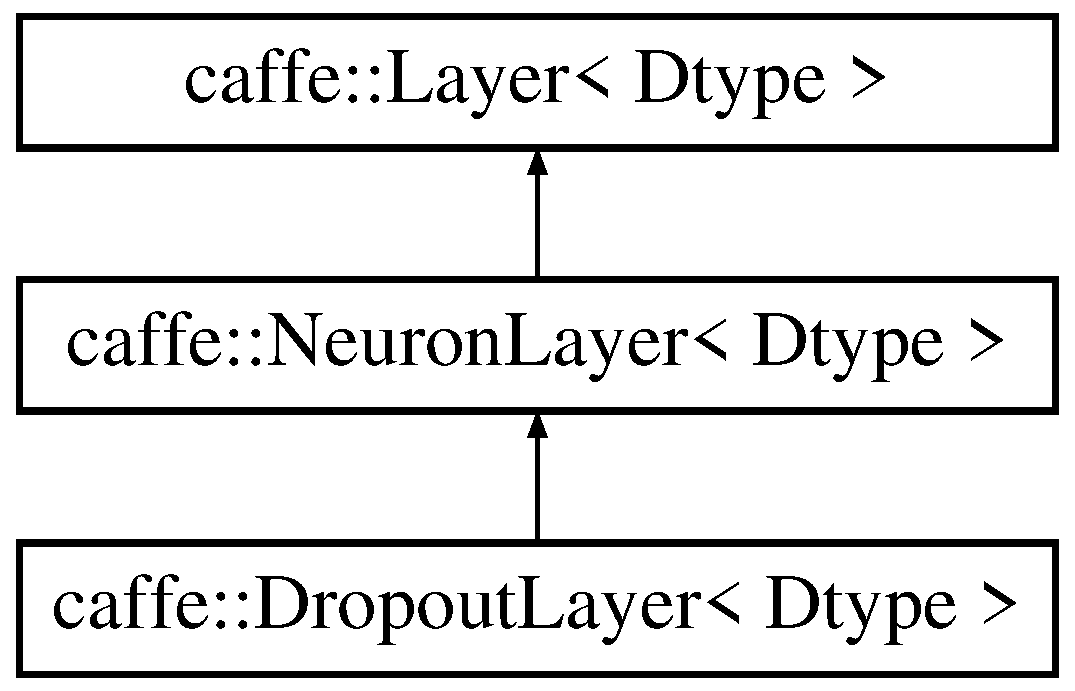
\includegraphics[height=3.000000cm]{classcaffe_1_1DropoutLayer}
\end{center}
\end{figure}
\subsection*{Public Member Functions}
\begin{DoxyCompactItemize}
\item 
\hyperlink{classcaffe_1_1DropoutLayer_a24cbddd4699b102a9555d3b8013c16d0}{Dropout\+Layer} (const Layer\+Parameter \&param)
\item 
virtual void \hyperlink{classcaffe_1_1DropoutLayer_a82bcd23115526808c79c807686945145}{Layer\+Set\+Up} (const vector$<$ \hyperlink{classcaffe_1_1Blob}{Blob}$<$ Dtype $>$ $\ast$ $>$ \&bottom, const vector$<$ \hyperlink{classcaffe_1_1Blob}{Blob}$<$ Dtype $>$ $\ast$ $>$ \&top)
\begin{DoxyCompactList}\small\item\em Does layer-\/specific setup\+: your layer should implement this function as well as Reshape. \end{DoxyCompactList}\item 
virtual void \hyperlink{classcaffe_1_1DropoutLayer_a3d5bce578b44ba2a89c1d4f7205ed842}{Reshape} (const vector$<$ \hyperlink{classcaffe_1_1Blob}{Blob}$<$ Dtype $>$ $\ast$ $>$ \&bottom, const vector$<$ \hyperlink{classcaffe_1_1Blob}{Blob}$<$ Dtype $>$ $\ast$ $>$ \&top)
\begin{DoxyCompactList}\small\item\em Adjust the shapes of top blobs and internal buffers to accommodate the shapes of the bottom blobs. \end{DoxyCompactList}\item 
virtual const char $\ast$ \hyperlink{classcaffe_1_1DropoutLayer_a73b1eba29e00cea48e1faaf9818b5dba}{type} () const \hypertarget{classcaffe_1_1DropoutLayer_a73b1eba29e00cea48e1faaf9818b5dba}{}\label{classcaffe_1_1DropoutLayer_a73b1eba29e00cea48e1faaf9818b5dba}

\begin{DoxyCompactList}\small\item\em Returns the layer type. \end{DoxyCompactList}\end{DoxyCompactItemize}
\subsection*{Protected Member Functions}
\begin{DoxyCompactItemize}
\item 
virtual void \hyperlink{classcaffe_1_1DropoutLayer_a0216a90061f76314ad9cbcff9a30de8c}{Forward\+\_\+cpu} (const vector$<$ \hyperlink{classcaffe_1_1Blob}{Blob}$<$ Dtype $>$ $\ast$ $>$ \&bottom, const vector$<$ \hyperlink{classcaffe_1_1Blob}{Blob}$<$ Dtype $>$ $\ast$ $>$ \&top)
\item 
virtual void \hyperlink{classcaffe_1_1DropoutLayer_ac5aa2af956f5860729cc168c71eaee06}{Forward\+\_\+gpu} (const vector$<$ \hyperlink{classcaffe_1_1Blob}{Blob}$<$ Dtype $>$ $\ast$ $>$ \&bottom, const vector$<$ \hyperlink{classcaffe_1_1Blob}{Blob}$<$ Dtype $>$ $\ast$ $>$ \&top)\hypertarget{classcaffe_1_1DropoutLayer_ac5aa2af956f5860729cc168c71eaee06}{}\label{classcaffe_1_1DropoutLayer_ac5aa2af956f5860729cc168c71eaee06}

\begin{DoxyCompactList}\small\item\em Using the G\+PU device, compute the layer output. Fall back to \hyperlink{classcaffe_1_1DropoutLayer_a0216a90061f76314ad9cbcff9a30de8c}{Forward\+\_\+cpu()} if unavailable. \end{DoxyCompactList}\item 
virtual void \hyperlink{classcaffe_1_1DropoutLayer_a867367c03a4ddada547c6f5d663cdc73}{Backward\+\_\+cpu} (const vector$<$ \hyperlink{classcaffe_1_1Blob}{Blob}$<$ Dtype $>$ $\ast$ $>$ \&top, const vector$<$ bool $>$ \&propagate\+\_\+down, const vector$<$ \hyperlink{classcaffe_1_1Blob}{Blob}$<$ Dtype $>$ $\ast$ $>$ \&bottom)\hypertarget{classcaffe_1_1DropoutLayer_a867367c03a4ddada547c6f5d663cdc73}{}\label{classcaffe_1_1DropoutLayer_a867367c03a4ddada547c6f5d663cdc73}

\begin{DoxyCompactList}\small\item\em Using the C\+PU device, compute the gradients for any parameters and for the bottom blobs if propagate\+\_\+down is true. \end{DoxyCompactList}\item 
virtual void \hyperlink{classcaffe_1_1DropoutLayer_a94686dbe949aee8316e905cc1d0dde2e}{Backward\+\_\+gpu} (const vector$<$ \hyperlink{classcaffe_1_1Blob}{Blob}$<$ Dtype $>$ $\ast$ $>$ \&top, const vector$<$ bool $>$ \&propagate\+\_\+down, const vector$<$ \hyperlink{classcaffe_1_1Blob}{Blob}$<$ Dtype $>$ $\ast$ $>$ \&bottom)\hypertarget{classcaffe_1_1DropoutLayer_a94686dbe949aee8316e905cc1d0dde2e}{}\label{classcaffe_1_1DropoutLayer_a94686dbe949aee8316e905cc1d0dde2e}

\begin{DoxyCompactList}\small\item\em Using the G\+PU device, compute the gradients for any parameters and for the bottom blobs if propagate\+\_\+down is true. Fall back to \hyperlink{classcaffe_1_1DropoutLayer_a867367c03a4ddada547c6f5d663cdc73}{Backward\+\_\+cpu()} if unavailable. \end{DoxyCompactList}\end{DoxyCompactItemize}
\subsection*{Protected Attributes}
\begin{DoxyCompactItemize}
\item 
\hyperlink{classcaffe_1_1Blob}{Blob}$<$ unsigned int $>$ \hyperlink{classcaffe_1_1DropoutLayer_a7a2c28420611a960a964e56acdbe2b47}{rand\+\_\+vec\+\_\+}\hypertarget{classcaffe_1_1DropoutLayer_a7a2c28420611a960a964e56acdbe2b47}{}\label{classcaffe_1_1DropoutLayer_a7a2c28420611a960a964e56acdbe2b47}

\begin{DoxyCompactList}\small\item\em when divided by U\+I\+N\+T\+\_\+\+M\+AX, the randomly generated values $u\sim U(0,1)$ \end{DoxyCompactList}\item 
Dtype \hyperlink{classcaffe_1_1DropoutLayer_a8e9d88e6128a97101c27ce8a11158ca6}{threshold\+\_\+}\hypertarget{classcaffe_1_1DropoutLayer_a8e9d88e6128a97101c27ce8a11158ca6}{}\label{classcaffe_1_1DropoutLayer_a8e9d88e6128a97101c27ce8a11158ca6}

\begin{DoxyCompactList}\small\item\em the probability $ p $ of dropping any input \end{DoxyCompactList}\item 
Dtype \hyperlink{classcaffe_1_1DropoutLayer_ac8702c053de0fea389f5a0ded8cdc544}{scale\+\_\+}\hypertarget{classcaffe_1_1DropoutLayer_ac8702c053de0fea389f5a0ded8cdc544}{}\label{classcaffe_1_1DropoutLayer_ac8702c053de0fea389f5a0ded8cdc544}

\begin{DoxyCompactList}\small\item\em the scale for undropped inputs at train time $ 1 / (1 - p) $ \end{DoxyCompactList}\item 
unsigned int {\bfseries uint\+\_\+thres\+\_\+}\hypertarget{classcaffe_1_1DropoutLayer_ae8ba2b98a7bc12643eec8ad72a66be21}{}\label{classcaffe_1_1DropoutLayer_ae8ba2b98a7bc12643eec8ad72a66be21}

\end{DoxyCompactItemize}


\subsection{Detailed Description}
\subsubsection*{template$<$typename Dtype$>$\\*
class caffe\+::\+Dropout\+Layer$<$ Dtype $>$}

During training only, sets a random portion of $x$ to 0, adjusting the rest of the vector magnitude accordingly. 


\begin{DoxyParams}{Parameters}
{\em bottom} & input \hyperlink{classcaffe_1_1Blob}{Blob} vector (length 1)
\begin{DoxyEnumerate}
\item $ (N \times C \times H \times W) $ the inputs $ x $ 
\end{DoxyEnumerate}\\
\hline
{\em top} & output \hyperlink{classcaffe_1_1Blob}{Blob} vector (length 1)
\begin{DoxyEnumerate}
\item $ (N \times C \times H \times W) $ the computed outputs $ y = |x| $ 
\end{DoxyEnumerate}\\
\hline
\end{DoxyParams}


\subsection{Constructor \& Destructor Documentation}
\index{caffe\+::\+Dropout\+Layer@{caffe\+::\+Dropout\+Layer}!Dropout\+Layer@{Dropout\+Layer}}
\index{Dropout\+Layer@{Dropout\+Layer}!caffe\+::\+Dropout\+Layer@{caffe\+::\+Dropout\+Layer}}
\subsubsection[{\texorpdfstring{Dropout\+Layer(const Layer\+Parameter \&param)}{DropoutLayer(const LayerParameter &param)}}]{\setlength{\rightskip}{0pt plus 5cm}template$<$typename Dtype $>$ {\bf caffe\+::\+Dropout\+Layer}$<$ Dtype $>$\+::{\bf Dropout\+Layer} (
\begin{DoxyParamCaption}
\item[{const Layer\+Parameter \&}]{param}
\end{DoxyParamCaption}
)\hspace{0.3cm}{\ttfamily [inline]}, {\ttfamily [explicit]}}\hypertarget{classcaffe_1_1DropoutLayer_a24cbddd4699b102a9555d3b8013c16d0}{}\label{classcaffe_1_1DropoutLayer_a24cbddd4699b102a9555d3b8013c16d0}

\begin{DoxyParams}{Parameters}
{\em param} & provides Dropout\+Parameter dropout\+\_\+param, with \hyperlink{classcaffe_1_1DropoutLayer}{Dropout\+Layer} options\+:
\begin{DoxyItemize}
\item dropout\+\_\+ratio ({\bfseries optional}, default 0.\+5). Sets the probability $ p $ that any given unit is dropped. 
\end{DoxyItemize}\\
\hline
\end{DoxyParams}


\subsection{Member Function Documentation}
\index{caffe\+::\+Dropout\+Layer@{caffe\+::\+Dropout\+Layer}!Forward\+\_\+cpu@{Forward\+\_\+cpu}}
\index{Forward\+\_\+cpu@{Forward\+\_\+cpu}!caffe\+::\+Dropout\+Layer@{caffe\+::\+Dropout\+Layer}}
\subsubsection[{\texorpdfstring{Forward\+\_\+cpu(const vector$<$ Blob$<$ Dtype $>$ $\ast$ $>$ \&bottom, const vector$<$ Blob$<$ Dtype $>$ $\ast$ $>$ \&top)}{Forward_cpu(const vector< Blob< Dtype > * > &bottom, const vector< Blob< Dtype > * > &top)}}]{\setlength{\rightskip}{0pt plus 5cm}template$<$typename Dtype $>$ void {\bf caffe\+::\+Dropout\+Layer}$<$ Dtype $>$\+::Forward\+\_\+cpu (
\begin{DoxyParamCaption}
\item[{const vector$<$ {\bf Blob}$<$ Dtype $>$ $\ast$ $>$ \&}]{bottom, }
\item[{const vector$<$ {\bf Blob}$<$ Dtype $>$ $\ast$ $>$ \&}]{top}
\end{DoxyParamCaption}
)\hspace{0.3cm}{\ttfamily [protected]}, {\ttfamily [virtual]}}\hypertarget{classcaffe_1_1DropoutLayer_a0216a90061f76314ad9cbcff9a30de8c}{}\label{classcaffe_1_1DropoutLayer_a0216a90061f76314ad9cbcff9a30de8c}

\begin{DoxyParams}{Parameters}
{\em bottom} & input \hyperlink{classcaffe_1_1Blob}{Blob} vector (length 1)
\begin{DoxyEnumerate}
\item $ (N \times C \times H \times W) $ the inputs $ x $ 
\end{DoxyEnumerate}\\
\hline
{\em top} & output \hyperlink{classcaffe_1_1Blob}{Blob} vector (length 1)
\begin{DoxyEnumerate}
\item $ (N \times C \times H \times W) $ the computed outputs. At training time, we have $ y_{\mbox{train}} = \left\{ \begin{array}{ll} \frac{x}{1 - p} & \mbox{if } u > p \\ 0 & \mbox{otherwise} \end{array} \right. $, where $ u \sim U(0, 1)$ is generated independently for each input at each iteration. At test time, we simply have $ y_{\mbox{test}} = \mathbb{E}[y_{\mbox{train}}] = x $. 
\end{DoxyEnumerate}\\
\hline
\end{DoxyParams}


Implements \hyperlink{classcaffe_1_1Layer_add965883f75bbf90c7a06f960cda7a1a}{caffe\+::\+Layer$<$ Dtype $>$}.

\index{caffe\+::\+Dropout\+Layer@{caffe\+::\+Dropout\+Layer}!Layer\+Set\+Up@{Layer\+Set\+Up}}
\index{Layer\+Set\+Up@{Layer\+Set\+Up}!caffe\+::\+Dropout\+Layer@{caffe\+::\+Dropout\+Layer}}
\subsubsection[{\texorpdfstring{Layer\+Set\+Up(const vector$<$ Blob$<$ Dtype $>$ $\ast$ $>$ \&bottom, const vector$<$ Blob$<$ Dtype $>$ $\ast$ $>$ \&top)}{LayerSetUp(const vector< Blob< Dtype > * > &bottom, const vector< Blob< Dtype > * > &top)}}]{\setlength{\rightskip}{0pt plus 5cm}template$<$typename Dtype $>$ void {\bf caffe\+::\+Dropout\+Layer}$<$ Dtype $>$\+::Layer\+Set\+Up (
\begin{DoxyParamCaption}
\item[{const vector$<$ {\bf Blob}$<$ Dtype $>$ $\ast$ $>$ \&}]{bottom, }
\item[{const vector$<$ {\bf Blob}$<$ Dtype $>$ $\ast$ $>$ \&}]{top}
\end{DoxyParamCaption}
)\hspace{0.3cm}{\ttfamily [virtual]}}\hypertarget{classcaffe_1_1DropoutLayer_a82bcd23115526808c79c807686945145}{}\label{classcaffe_1_1DropoutLayer_a82bcd23115526808c79c807686945145}


Does layer-\/specific setup\+: your layer should implement this function as well as Reshape. 


\begin{DoxyParams}{Parameters}
{\em bottom} & the preshaped input blobs, whose data fields store the input data for this layer \\
\hline
{\em top} & the allocated but unshaped output blobs\\
\hline
\end{DoxyParams}
This method should do one-\/time layer specific setup. This includes reading and processing relevent parameters from the {\ttfamily layer\+\_\+param\+\_\+}. Setting up the shapes of top blobs and internal buffers should be done in {\ttfamily Reshape}, which will be called before the forward pass to adjust the top blob sizes. 

Reimplemented from \hyperlink{classcaffe_1_1Layer_a38dc2488bf319b8de5a7ac84e0045393}{caffe\+::\+Layer$<$ Dtype $>$}.

\index{caffe\+::\+Dropout\+Layer@{caffe\+::\+Dropout\+Layer}!Reshape@{Reshape}}
\index{Reshape@{Reshape}!caffe\+::\+Dropout\+Layer@{caffe\+::\+Dropout\+Layer}}
\subsubsection[{\texorpdfstring{Reshape(const vector$<$ Blob$<$ Dtype $>$ $\ast$ $>$ \&bottom, const vector$<$ Blob$<$ Dtype $>$ $\ast$ $>$ \&top)}{Reshape(const vector< Blob< Dtype > * > &bottom, const vector< Blob< Dtype > * > &top)}}]{\setlength{\rightskip}{0pt plus 5cm}template$<$typename Dtype $>$ void {\bf caffe\+::\+Dropout\+Layer}$<$ Dtype $>$\+::Reshape (
\begin{DoxyParamCaption}
\item[{const vector$<$ {\bf Blob}$<$ Dtype $>$ $\ast$ $>$ \&}]{bottom, }
\item[{const vector$<$ {\bf Blob}$<$ Dtype $>$ $\ast$ $>$ \&}]{top}
\end{DoxyParamCaption}
)\hspace{0.3cm}{\ttfamily [virtual]}}\hypertarget{classcaffe_1_1DropoutLayer_a3d5bce578b44ba2a89c1d4f7205ed842}{}\label{classcaffe_1_1DropoutLayer_a3d5bce578b44ba2a89c1d4f7205ed842}


Adjust the shapes of top blobs and internal buffers to accommodate the shapes of the bottom blobs. 


\begin{DoxyParams}{Parameters}
{\em bottom} & the input blobs, with the requested input shapes \\
\hline
{\em top} & the top blobs, which should be reshaped as needed\\
\hline
\end{DoxyParams}
This method should reshape top blobs as needed according to the shapes of the bottom (input) blobs, as well as reshaping any internal buffers and making any other necessary adjustments so that the layer can accommodate the bottom blobs. 

Reimplemented from \hyperlink{classcaffe_1_1NeuronLayer_a810f5f75b95ba7fdcb9d3e0e33e98a7e}{caffe\+::\+Neuron\+Layer$<$ Dtype $>$}.



The documentation for this class was generated from the following files\+:\begin{DoxyCompactItemize}
\item 
include/caffe/layers/dropout\+\_\+layer.\+hpp\item 
src/caffe/layers/dropout\+\_\+layer.\+cpp\end{DoxyCompactItemize}

\hypertarget{classcaffe_1_1DummyDataLayer}{}\section{caffe\+:\+:Dummy\+Data\+Layer$<$ Dtype $>$ Class Template Reference}
\label{classcaffe_1_1DummyDataLayer}\index{caffe\+::\+Dummy\+Data\+Layer$<$ Dtype $>$@{caffe\+::\+Dummy\+Data\+Layer$<$ Dtype $>$}}


Provides data to the \hyperlink{classcaffe_1_1Net}{Net} generated by a \hyperlink{classcaffe_1_1Filler}{Filler}.  




{\ttfamily \#include $<$dummy\+\_\+data\+\_\+layer.\+hpp$>$}

Inheritance diagram for caffe\+:\+:Dummy\+Data\+Layer$<$ Dtype $>$\+:\begin{figure}[H]
\begin{center}
\leavevmode
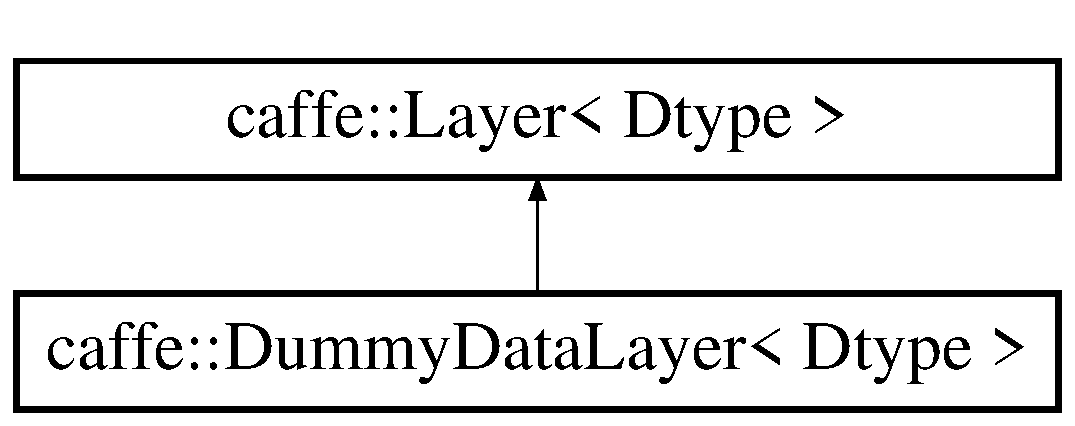
\includegraphics[height=2.000000cm]{classcaffe_1_1DummyDataLayer}
\end{center}
\end{figure}
\subsection*{Public Member Functions}
\begin{DoxyCompactItemize}
\item 
{\bfseries Dummy\+Data\+Layer} (const Layer\+Parameter \&param)\hypertarget{classcaffe_1_1DummyDataLayer_a98568bcfa177c5eef82ebd0f50465c78}{}\label{classcaffe_1_1DummyDataLayer_a98568bcfa177c5eef82ebd0f50465c78}

\item 
virtual void \hyperlink{classcaffe_1_1DummyDataLayer_a7469fb111146a3f2a3121a3f1adb2c31}{Layer\+Set\+Up} (const vector$<$ \hyperlink{classcaffe_1_1Blob}{Blob}$<$ Dtype $>$ $\ast$ $>$ \&bottom, const vector$<$ \hyperlink{classcaffe_1_1Blob}{Blob}$<$ Dtype $>$ $\ast$ $>$ \&top)
\begin{DoxyCompactList}\small\item\em Does layer-\/specific setup\+: your layer should implement this function as well as Reshape. \end{DoxyCompactList}\item 
virtual void \hyperlink{classcaffe_1_1DummyDataLayer_ab05d22a6458132c47488cdf2f53a0104}{Reshape} (const vector$<$ \hyperlink{classcaffe_1_1Blob}{Blob}$<$ Dtype $>$ $\ast$ $>$ \&bottom, const vector$<$ \hyperlink{classcaffe_1_1Blob}{Blob}$<$ Dtype $>$ $\ast$ $>$ \&top)
\begin{DoxyCompactList}\small\item\em Adjust the shapes of top blobs and internal buffers to accommodate the shapes of the bottom blobs. \end{DoxyCompactList}\item 
virtual const char $\ast$ \hyperlink{classcaffe_1_1DummyDataLayer_ad3274d1aacd5ce73f6fcf15de15a1784}{type} () const \hypertarget{classcaffe_1_1DummyDataLayer_ad3274d1aacd5ce73f6fcf15de15a1784}{}\label{classcaffe_1_1DummyDataLayer_ad3274d1aacd5ce73f6fcf15de15a1784}

\begin{DoxyCompactList}\small\item\em Returns the layer type. \end{DoxyCompactList}\item 
virtual int \hyperlink{classcaffe_1_1DummyDataLayer_ad25325d52be96802665c21acc792c6dc}{Exact\+Num\+Bottom\+Blobs} () const 
\begin{DoxyCompactList}\small\item\em Returns the exact number of bottom blobs required by the layer, or -\/1 if no exact number is required. \end{DoxyCompactList}\item 
virtual int \hyperlink{classcaffe_1_1DummyDataLayer_a82dba92b339f5d1e0d987fae8d47cd02}{Min\+Top\+Blobs} () const 
\begin{DoxyCompactList}\small\item\em Returns the minimum number of top blobs required by the layer, or -\/1 if no minimum number is required. \end{DoxyCompactList}\end{DoxyCompactItemize}
\subsection*{Protected Member Functions}
\begin{DoxyCompactItemize}
\item 
virtual void \hyperlink{classcaffe_1_1DummyDataLayer_af9b443837b9b8a7e6942df57878d5fd9}{Forward\+\_\+cpu} (const vector$<$ \hyperlink{classcaffe_1_1Blob}{Blob}$<$ Dtype $>$ $\ast$ $>$ \&bottom, const vector$<$ \hyperlink{classcaffe_1_1Blob}{Blob}$<$ Dtype $>$ $\ast$ $>$ \&top)\hypertarget{classcaffe_1_1DummyDataLayer_af9b443837b9b8a7e6942df57878d5fd9}{}\label{classcaffe_1_1DummyDataLayer_af9b443837b9b8a7e6942df57878d5fd9}

\begin{DoxyCompactList}\small\item\em Using the C\+PU device, compute the layer output. \end{DoxyCompactList}\item 
virtual void \hyperlink{classcaffe_1_1DummyDataLayer_a127c0630147b43c4c99b107e4997128d}{Backward\+\_\+cpu} (const vector$<$ \hyperlink{classcaffe_1_1Blob}{Blob}$<$ Dtype $>$ $\ast$ $>$ \&top, const vector$<$ bool $>$ \&propagate\+\_\+down, const vector$<$ \hyperlink{classcaffe_1_1Blob}{Blob}$<$ Dtype $>$ $\ast$ $>$ \&bottom)\hypertarget{classcaffe_1_1DummyDataLayer_a127c0630147b43c4c99b107e4997128d}{}\label{classcaffe_1_1DummyDataLayer_a127c0630147b43c4c99b107e4997128d}

\begin{DoxyCompactList}\small\item\em Using the C\+PU device, compute the gradients for any parameters and for the bottom blobs if propagate\+\_\+down is true. \end{DoxyCompactList}\item 
virtual void \hyperlink{classcaffe_1_1DummyDataLayer_adda172e0787cae45c1d6a162de1e5a28}{Backward\+\_\+gpu} (const vector$<$ \hyperlink{classcaffe_1_1Blob}{Blob}$<$ Dtype $>$ $\ast$ $>$ \&top, const vector$<$ bool $>$ \&propagate\+\_\+down, const vector$<$ \hyperlink{classcaffe_1_1Blob}{Blob}$<$ Dtype $>$ $\ast$ $>$ \&bottom)\hypertarget{classcaffe_1_1DummyDataLayer_adda172e0787cae45c1d6a162de1e5a28}{}\label{classcaffe_1_1DummyDataLayer_adda172e0787cae45c1d6a162de1e5a28}

\begin{DoxyCompactList}\small\item\em Using the G\+PU device, compute the gradients for any parameters and for the bottom blobs if propagate\+\_\+down is true. Fall back to \hyperlink{classcaffe_1_1DummyDataLayer_a127c0630147b43c4c99b107e4997128d}{Backward\+\_\+cpu()} if unavailable. \end{DoxyCompactList}\end{DoxyCompactItemize}
\subsection*{Protected Attributes}
\begin{DoxyCompactItemize}
\item 
vector$<$ shared\+\_\+ptr$<$ \hyperlink{classcaffe_1_1Filler}{Filler}$<$ Dtype $>$ $>$ $>$ {\bfseries fillers\+\_\+}\hypertarget{classcaffe_1_1DummyDataLayer_afdc9cd76ff63c6ff40d1f92585b0906e}{}\label{classcaffe_1_1DummyDataLayer_afdc9cd76ff63c6ff40d1f92585b0906e}

\item 
vector$<$ bool $>$ {\bfseries refill\+\_\+}\hypertarget{classcaffe_1_1DummyDataLayer_a4ea3c6bbb0fbe48558ed0a762df56add}{}\label{classcaffe_1_1DummyDataLayer_a4ea3c6bbb0fbe48558ed0a762df56add}

\end{DoxyCompactItemize}


\subsection{Detailed Description}
\subsubsection*{template$<$typename Dtype$>$\\*
class caffe\+::\+Dummy\+Data\+Layer$<$ Dtype $>$}

Provides data to the \hyperlink{classcaffe_1_1Net}{Net} generated by a \hyperlink{classcaffe_1_1Filler}{Filler}. 

T\+O\+D\+O(dox)\+: thorough documentation for Forward and proto params. 

\subsection{Member Function Documentation}
\index{caffe\+::\+Dummy\+Data\+Layer@{caffe\+::\+Dummy\+Data\+Layer}!Exact\+Num\+Bottom\+Blobs@{Exact\+Num\+Bottom\+Blobs}}
\index{Exact\+Num\+Bottom\+Blobs@{Exact\+Num\+Bottom\+Blobs}!caffe\+::\+Dummy\+Data\+Layer@{caffe\+::\+Dummy\+Data\+Layer}}
\subsubsection[{\texorpdfstring{Exact\+Num\+Bottom\+Blobs() const }{ExactNumBottomBlobs() const }}]{\setlength{\rightskip}{0pt plus 5cm}template$<$typename Dtype $>$ virtual int {\bf caffe\+::\+Dummy\+Data\+Layer}$<$ Dtype $>$\+::Exact\+Num\+Bottom\+Blobs (
\begin{DoxyParamCaption}
{}
\end{DoxyParamCaption}
) const\hspace{0.3cm}{\ttfamily [inline]}, {\ttfamily [virtual]}}\hypertarget{classcaffe_1_1DummyDataLayer_ad25325d52be96802665c21acc792c6dc}{}\label{classcaffe_1_1DummyDataLayer_ad25325d52be96802665c21acc792c6dc}


Returns the exact number of bottom blobs required by the layer, or -\/1 if no exact number is required. 

This method should be overridden to return a non-\/negative value if your layer expects some exact number of bottom blobs. 

Reimplemented from \hyperlink{classcaffe_1_1Layer_a45c7a7943a8a6735ac433c9be11e0240}{caffe\+::\+Layer$<$ Dtype $>$}.

\index{caffe\+::\+Dummy\+Data\+Layer@{caffe\+::\+Dummy\+Data\+Layer}!Layer\+Set\+Up@{Layer\+Set\+Up}}
\index{Layer\+Set\+Up@{Layer\+Set\+Up}!caffe\+::\+Dummy\+Data\+Layer@{caffe\+::\+Dummy\+Data\+Layer}}
\subsubsection[{\texorpdfstring{Layer\+Set\+Up(const vector$<$ Blob$<$ Dtype $>$ $\ast$ $>$ \&bottom, const vector$<$ Blob$<$ Dtype $>$ $\ast$ $>$ \&top)}{LayerSetUp(const vector< Blob< Dtype > * > &bottom, const vector< Blob< Dtype > * > &top)}}]{\setlength{\rightskip}{0pt plus 5cm}template$<$typename Dtype $>$ void {\bf caffe\+::\+Dummy\+Data\+Layer}$<$ Dtype $>$\+::Layer\+Set\+Up (
\begin{DoxyParamCaption}
\item[{const vector$<$ {\bf Blob}$<$ Dtype $>$ $\ast$ $>$ \&}]{bottom, }
\item[{const vector$<$ {\bf Blob}$<$ Dtype $>$ $\ast$ $>$ \&}]{top}
\end{DoxyParamCaption}
)\hspace{0.3cm}{\ttfamily [virtual]}}\hypertarget{classcaffe_1_1DummyDataLayer_a7469fb111146a3f2a3121a3f1adb2c31}{}\label{classcaffe_1_1DummyDataLayer_a7469fb111146a3f2a3121a3f1adb2c31}


Does layer-\/specific setup\+: your layer should implement this function as well as Reshape. 


\begin{DoxyParams}{Parameters}
{\em bottom} & the preshaped input blobs, whose data fields store the input data for this layer \\
\hline
{\em top} & the allocated but unshaped output blobs\\
\hline
\end{DoxyParams}
This method should do one-\/time layer specific setup. This includes reading and processing relevent parameters from the {\ttfamily layer\+\_\+param\+\_\+}. Setting up the shapes of top blobs and internal buffers should be done in {\ttfamily Reshape}, which will be called before the forward pass to adjust the top blob sizes. 

Reimplemented from \hyperlink{classcaffe_1_1Layer_a38dc2488bf319b8de5a7ac84e0045393}{caffe\+::\+Layer$<$ Dtype $>$}.

\index{caffe\+::\+Dummy\+Data\+Layer@{caffe\+::\+Dummy\+Data\+Layer}!Min\+Top\+Blobs@{Min\+Top\+Blobs}}
\index{Min\+Top\+Blobs@{Min\+Top\+Blobs}!caffe\+::\+Dummy\+Data\+Layer@{caffe\+::\+Dummy\+Data\+Layer}}
\subsubsection[{\texorpdfstring{Min\+Top\+Blobs() const }{MinTopBlobs() const }}]{\setlength{\rightskip}{0pt plus 5cm}template$<$typename Dtype $>$ virtual int {\bf caffe\+::\+Dummy\+Data\+Layer}$<$ Dtype $>$\+::Min\+Top\+Blobs (
\begin{DoxyParamCaption}
{}
\end{DoxyParamCaption}
) const\hspace{0.3cm}{\ttfamily [inline]}, {\ttfamily [virtual]}}\hypertarget{classcaffe_1_1DummyDataLayer_a82dba92b339f5d1e0d987fae8d47cd02}{}\label{classcaffe_1_1DummyDataLayer_a82dba92b339f5d1e0d987fae8d47cd02}


Returns the minimum number of top blobs required by the layer, or -\/1 if no minimum number is required. 

This method should be overridden to return a non-\/negative value if your layer expects some minimum number of top blobs. 

Reimplemented from \hyperlink{classcaffe_1_1Layer_a8bb143d58a740345fa2dc3d4204d553b}{caffe\+::\+Layer$<$ Dtype $>$}.

\index{caffe\+::\+Dummy\+Data\+Layer@{caffe\+::\+Dummy\+Data\+Layer}!Reshape@{Reshape}}
\index{Reshape@{Reshape}!caffe\+::\+Dummy\+Data\+Layer@{caffe\+::\+Dummy\+Data\+Layer}}
\subsubsection[{\texorpdfstring{Reshape(const vector$<$ Blob$<$ Dtype $>$ $\ast$ $>$ \&bottom, const vector$<$ Blob$<$ Dtype $>$ $\ast$ $>$ \&top)}{Reshape(const vector< Blob< Dtype > * > &bottom, const vector< Blob< Dtype > * > &top)}}]{\setlength{\rightskip}{0pt plus 5cm}template$<$typename Dtype $>$ virtual void {\bf caffe\+::\+Dummy\+Data\+Layer}$<$ Dtype $>$\+::Reshape (
\begin{DoxyParamCaption}
\item[{const vector$<$ {\bf Blob}$<$ Dtype $>$ $\ast$ $>$ \&}]{bottom, }
\item[{const vector$<$ {\bf Blob}$<$ Dtype $>$ $\ast$ $>$ \&}]{top}
\end{DoxyParamCaption}
)\hspace{0.3cm}{\ttfamily [inline]}, {\ttfamily [virtual]}}\hypertarget{classcaffe_1_1DummyDataLayer_ab05d22a6458132c47488cdf2f53a0104}{}\label{classcaffe_1_1DummyDataLayer_ab05d22a6458132c47488cdf2f53a0104}


Adjust the shapes of top blobs and internal buffers to accommodate the shapes of the bottom blobs. 


\begin{DoxyParams}{Parameters}
{\em bottom} & the input blobs, with the requested input shapes \\
\hline
{\em top} & the top blobs, which should be reshaped as needed\\
\hline
\end{DoxyParams}
This method should reshape top blobs as needed according to the shapes of the bottom (input) blobs, as well as reshaping any internal buffers and making any other necessary adjustments so that the layer can accommodate the bottom blobs. 

Implements \hyperlink{classcaffe_1_1Layer_ad9d391b972c769c0ebee34ca6d1c973e}{caffe\+::\+Layer$<$ Dtype $>$}.



The documentation for this class was generated from the following files\+:\begin{DoxyCompactItemize}
\item 
include/caffe/layers/dummy\+\_\+data\+\_\+layer.\+hpp\item 
src/caffe/layers/dummy\+\_\+data\+\_\+layer.\+cpp\end{DoxyCompactItemize}

\hypertarget{classcaffe_1_1EltwiseLayer}{}\section{caffe\+:\+:Eltwise\+Layer$<$ Dtype $>$ Class Template Reference}
\label{classcaffe_1_1EltwiseLayer}\index{caffe\+::\+Eltwise\+Layer$<$ Dtype $>$@{caffe\+::\+Eltwise\+Layer$<$ Dtype $>$}}


Compute elementwise operations, such as product and sum, along multiple input Blobs.  




{\ttfamily \#include $<$eltwise\+\_\+layer.\+hpp$>$}

Inheritance diagram for caffe\+:\+:Eltwise\+Layer$<$ Dtype $>$\+:\begin{figure}[H]
\begin{center}
\leavevmode
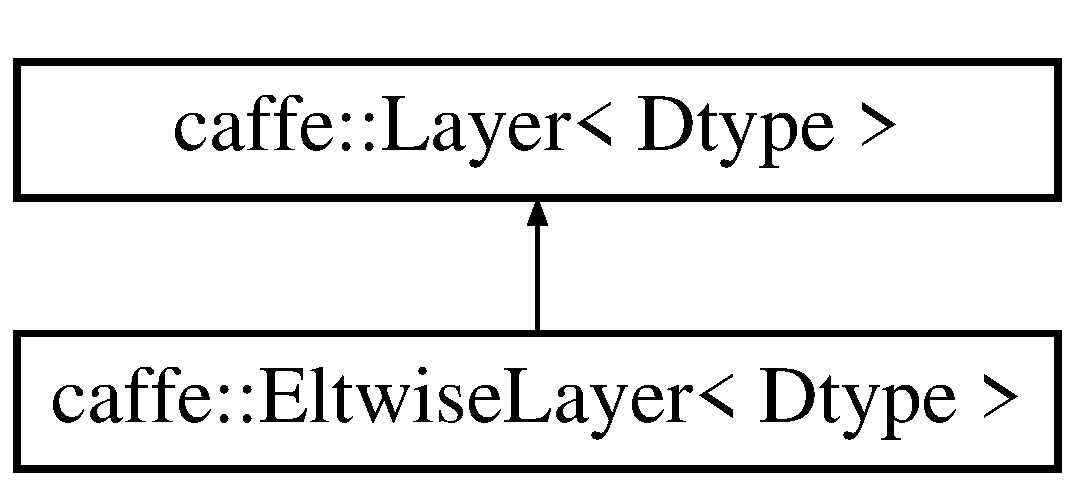
\includegraphics[height=2.000000cm]{classcaffe_1_1EltwiseLayer}
\end{center}
\end{figure}
\subsection*{Public Member Functions}
\begin{DoxyCompactItemize}
\item 
{\bfseries Eltwise\+Layer} (const Layer\+Parameter \&param)\hypertarget{classcaffe_1_1EltwiseLayer_a896ae6914a6358a90e3e67621a6fe082}{}\label{classcaffe_1_1EltwiseLayer_a896ae6914a6358a90e3e67621a6fe082}

\item 
virtual void \hyperlink{classcaffe_1_1EltwiseLayer_af4955762e92edb355b4f724e7ffd6473}{Layer\+Set\+Up} (const vector$<$ \hyperlink{classcaffe_1_1Blob}{Blob}$<$ Dtype $>$ $\ast$ $>$ \&bottom, const vector$<$ \hyperlink{classcaffe_1_1Blob}{Blob}$<$ Dtype $>$ $\ast$ $>$ \&top)
\begin{DoxyCompactList}\small\item\em Does layer-\/specific setup\+: your layer should implement this function as well as Reshape. \end{DoxyCompactList}\item 
virtual void \hyperlink{classcaffe_1_1EltwiseLayer_af5a843a83dda78e077ec580032ffd293}{Reshape} (const vector$<$ \hyperlink{classcaffe_1_1Blob}{Blob}$<$ Dtype $>$ $\ast$ $>$ \&bottom, const vector$<$ \hyperlink{classcaffe_1_1Blob}{Blob}$<$ Dtype $>$ $\ast$ $>$ \&top)
\begin{DoxyCompactList}\small\item\em Adjust the shapes of top blobs and internal buffers to accommodate the shapes of the bottom blobs. \end{DoxyCompactList}\item 
virtual const char $\ast$ \hyperlink{classcaffe_1_1EltwiseLayer_a425afe450f5b2fd9a17a944781ed9a3c}{type} () const \hypertarget{classcaffe_1_1EltwiseLayer_a425afe450f5b2fd9a17a944781ed9a3c}{}\label{classcaffe_1_1EltwiseLayer_a425afe450f5b2fd9a17a944781ed9a3c}

\begin{DoxyCompactList}\small\item\em Returns the layer type. \end{DoxyCompactList}\item 
virtual int \hyperlink{classcaffe_1_1EltwiseLayer_a27e853f4eb0e05ce52f9a3e291d06063}{Min\+Bottom\+Blobs} () const 
\begin{DoxyCompactList}\small\item\em Returns the minimum number of bottom blobs required by the layer, or -\/1 if no minimum number is required. \end{DoxyCompactList}\item 
virtual int \hyperlink{classcaffe_1_1EltwiseLayer_adab35a7e096edeb73670e6682f264774}{Exact\+Num\+Top\+Blobs} () const 
\begin{DoxyCompactList}\small\item\em Returns the exact number of top blobs required by the layer, or -\/1 if no exact number is required. \end{DoxyCompactList}\end{DoxyCompactItemize}
\subsection*{Protected Member Functions}
\begin{DoxyCompactItemize}
\item 
virtual void \hyperlink{classcaffe_1_1EltwiseLayer_adb87fdc9f21a9442178f956c14568db8}{Forward\+\_\+cpu} (const vector$<$ \hyperlink{classcaffe_1_1Blob}{Blob}$<$ Dtype $>$ $\ast$ $>$ \&bottom, const vector$<$ \hyperlink{classcaffe_1_1Blob}{Blob}$<$ Dtype $>$ $\ast$ $>$ \&top)\hypertarget{classcaffe_1_1EltwiseLayer_adb87fdc9f21a9442178f956c14568db8}{}\label{classcaffe_1_1EltwiseLayer_adb87fdc9f21a9442178f956c14568db8}

\begin{DoxyCompactList}\small\item\em Using the C\+PU device, compute the layer output. \end{DoxyCompactList}\item 
virtual void \hyperlink{classcaffe_1_1EltwiseLayer_a91acae1050d7fe61235ed84092231b07}{Forward\+\_\+gpu} (const vector$<$ \hyperlink{classcaffe_1_1Blob}{Blob}$<$ Dtype $>$ $\ast$ $>$ \&bottom, const vector$<$ \hyperlink{classcaffe_1_1Blob}{Blob}$<$ Dtype $>$ $\ast$ $>$ \&top)\hypertarget{classcaffe_1_1EltwiseLayer_a91acae1050d7fe61235ed84092231b07}{}\label{classcaffe_1_1EltwiseLayer_a91acae1050d7fe61235ed84092231b07}

\begin{DoxyCompactList}\small\item\em Using the G\+PU device, compute the layer output. Fall back to \hyperlink{classcaffe_1_1EltwiseLayer_adb87fdc9f21a9442178f956c14568db8}{Forward\+\_\+cpu()} if unavailable. \end{DoxyCompactList}\item 
virtual void \hyperlink{classcaffe_1_1EltwiseLayer_a2de367dcbd2da7fc6915ea4c133f6c3c}{Backward\+\_\+cpu} (const vector$<$ \hyperlink{classcaffe_1_1Blob}{Blob}$<$ Dtype $>$ $\ast$ $>$ \&top, const vector$<$ bool $>$ \&propagate\+\_\+down, const vector$<$ \hyperlink{classcaffe_1_1Blob}{Blob}$<$ Dtype $>$ $\ast$ $>$ \&bottom)\hypertarget{classcaffe_1_1EltwiseLayer_a2de367dcbd2da7fc6915ea4c133f6c3c}{}\label{classcaffe_1_1EltwiseLayer_a2de367dcbd2da7fc6915ea4c133f6c3c}

\begin{DoxyCompactList}\small\item\em Using the C\+PU device, compute the gradients for any parameters and for the bottom blobs if propagate\+\_\+down is true. \end{DoxyCompactList}\item 
virtual void \hyperlink{classcaffe_1_1EltwiseLayer_af102f2cb915289498c8040f697fdc10e}{Backward\+\_\+gpu} (const vector$<$ \hyperlink{classcaffe_1_1Blob}{Blob}$<$ Dtype $>$ $\ast$ $>$ \&top, const vector$<$ bool $>$ \&propagate\+\_\+down, const vector$<$ \hyperlink{classcaffe_1_1Blob}{Blob}$<$ Dtype $>$ $\ast$ $>$ \&bottom)\hypertarget{classcaffe_1_1EltwiseLayer_af102f2cb915289498c8040f697fdc10e}{}\label{classcaffe_1_1EltwiseLayer_af102f2cb915289498c8040f697fdc10e}

\begin{DoxyCompactList}\small\item\em Using the G\+PU device, compute the gradients for any parameters and for the bottom blobs if propagate\+\_\+down is true. Fall back to \hyperlink{classcaffe_1_1EltwiseLayer_a2de367dcbd2da7fc6915ea4c133f6c3c}{Backward\+\_\+cpu()} if unavailable. \end{DoxyCompactList}\end{DoxyCompactItemize}
\subsection*{Protected Attributes}
\begin{DoxyCompactItemize}
\item 
Eltwise\+Parameter\+\_\+\+Eltwise\+Op {\bfseries op\+\_\+}\hypertarget{classcaffe_1_1EltwiseLayer_a31a6111895a4ba616da848bde583f843}{}\label{classcaffe_1_1EltwiseLayer_a31a6111895a4ba616da848bde583f843}

\item 
vector$<$ Dtype $>$ {\bfseries coeffs\+\_\+}\hypertarget{classcaffe_1_1EltwiseLayer_a6096e37b3bd8fbfe5f2a5b6acc8cd608}{}\label{classcaffe_1_1EltwiseLayer_a6096e37b3bd8fbfe5f2a5b6acc8cd608}

\item 
\hyperlink{classcaffe_1_1Blob}{Blob}$<$ int $>$ {\bfseries max\+\_\+idx\+\_\+}\hypertarget{classcaffe_1_1EltwiseLayer_af1fe1e42da04da8073e80ca8bbb0e0de}{}\label{classcaffe_1_1EltwiseLayer_af1fe1e42da04da8073e80ca8bbb0e0de}

\item 
bool {\bfseries stable\+\_\+prod\+\_\+grad\+\_\+}\hypertarget{classcaffe_1_1EltwiseLayer_a94a93d8257e6b36431e83cc3a030e904}{}\label{classcaffe_1_1EltwiseLayer_a94a93d8257e6b36431e83cc3a030e904}

\end{DoxyCompactItemize}


\subsection{Detailed Description}
\subsubsection*{template$<$typename Dtype$>$\\*
class caffe\+::\+Eltwise\+Layer$<$ Dtype $>$}

Compute elementwise operations, such as product and sum, along multiple input Blobs. 

T\+O\+D\+O(dox)\+: thorough documentation for Forward, Backward, and proto params. 

\subsection{Member Function Documentation}
\index{caffe\+::\+Eltwise\+Layer@{caffe\+::\+Eltwise\+Layer}!Exact\+Num\+Top\+Blobs@{Exact\+Num\+Top\+Blobs}}
\index{Exact\+Num\+Top\+Blobs@{Exact\+Num\+Top\+Blobs}!caffe\+::\+Eltwise\+Layer@{caffe\+::\+Eltwise\+Layer}}
\subsubsection[{\texorpdfstring{Exact\+Num\+Top\+Blobs() const }{ExactNumTopBlobs() const }}]{\setlength{\rightskip}{0pt plus 5cm}template$<$typename Dtype $>$ virtual int {\bf caffe\+::\+Eltwise\+Layer}$<$ Dtype $>$\+::Exact\+Num\+Top\+Blobs (
\begin{DoxyParamCaption}
{}
\end{DoxyParamCaption}
) const\hspace{0.3cm}{\ttfamily [inline]}, {\ttfamily [virtual]}}\hypertarget{classcaffe_1_1EltwiseLayer_adab35a7e096edeb73670e6682f264774}{}\label{classcaffe_1_1EltwiseLayer_adab35a7e096edeb73670e6682f264774}


Returns the exact number of top blobs required by the layer, or -\/1 if no exact number is required. 

This method should be overridden to return a non-\/negative value if your layer expects some exact number of top blobs. 

Reimplemented from \hyperlink{classcaffe_1_1Layer_aa3c99ed707e8db683a3043412e151af8}{caffe\+::\+Layer$<$ Dtype $>$}.

\index{caffe\+::\+Eltwise\+Layer@{caffe\+::\+Eltwise\+Layer}!Layer\+Set\+Up@{Layer\+Set\+Up}}
\index{Layer\+Set\+Up@{Layer\+Set\+Up}!caffe\+::\+Eltwise\+Layer@{caffe\+::\+Eltwise\+Layer}}
\subsubsection[{\texorpdfstring{Layer\+Set\+Up(const vector$<$ Blob$<$ Dtype $>$ $\ast$ $>$ \&bottom, const vector$<$ Blob$<$ Dtype $>$ $\ast$ $>$ \&top)}{LayerSetUp(const vector< Blob< Dtype > * > &bottom, const vector< Blob< Dtype > * > &top)}}]{\setlength{\rightskip}{0pt plus 5cm}template$<$typename Dtype $>$ void {\bf caffe\+::\+Eltwise\+Layer}$<$ Dtype $>$\+::Layer\+Set\+Up (
\begin{DoxyParamCaption}
\item[{const vector$<$ {\bf Blob}$<$ Dtype $>$ $\ast$ $>$ \&}]{bottom, }
\item[{const vector$<$ {\bf Blob}$<$ Dtype $>$ $\ast$ $>$ \&}]{top}
\end{DoxyParamCaption}
)\hspace{0.3cm}{\ttfamily [virtual]}}\hypertarget{classcaffe_1_1EltwiseLayer_af4955762e92edb355b4f724e7ffd6473}{}\label{classcaffe_1_1EltwiseLayer_af4955762e92edb355b4f724e7ffd6473}


Does layer-\/specific setup\+: your layer should implement this function as well as Reshape. 


\begin{DoxyParams}{Parameters}
{\em bottom} & the preshaped input blobs, whose data fields store the input data for this layer \\
\hline
{\em top} & the allocated but unshaped output blobs\\
\hline
\end{DoxyParams}
This method should do one-\/time layer specific setup. This includes reading and processing relevent parameters from the {\ttfamily layer\+\_\+param\+\_\+}. Setting up the shapes of top blobs and internal buffers should be done in {\ttfamily Reshape}, which will be called before the forward pass to adjust the top blob sizes. 

Reimplemented from \hyperlink{classcaffe_1_1Layer_a38dc2488bf319b8de5a7ac84e0045393}{caffe\+::\+Layer$<$ Dtype $>$}.

\index{caffe\+::\+Eltwise\+Layer@{caffe\+::\+Eltwise\+Layer}!Min\+Bottom\+Blobs@{Min\+Bottom\+Blobs}}
\index{Min\+Bottom\+Blobs@{Min\+Bottom\+Blobs}!caffe\+::\+Eltwise\+Layer@{caffe\+::\+Eltwise\+Layer}}
\subsubsection[{\texorpdfstring{Min\+Bottom\+Blobs() const }{MinBottomBlobs() const }}]{\setlength{\rightskip}{0pt plus 5cm}template$<$typename Dtype $>$ virtual int {\bf caffe\+::\+Eltwise\+Layer}$<$ Dtype $>$\+::Min\+Bottom\+Blobs (
\begin{DoxyParamCaption}
{}
\end{DoxyParamCaption}
) const\hspace{0.3cm}{\ttfamily [inline]}, {\ttfamily [virtual]}}\hypertarget{classcaffe_1_1EltwiseLayer_a27e853f4eb0e05ce52f9a3e291d06063}{}\label{classcaffe_1_1EltwiseLayer_a27e853f4eb0e05ce52f9a3e291d06063}


Returns the minimum number of bottom blobs required by the layer, or -\/1 if no minimum number is required. 

This method should be overridden to return a non-\/negative value if your layer expects some minimum number of bottom blobs. 

Reimplemented from \hyperlink{classcaffe_1_1Layer_ade3eee97cc743c4e68fff7eba6484916}{caffe\+::\+Layer$<$ Dtype $>$}.

\index{caffe\+::\+Eltwise\+Layer@{caffe\+::\+Eltwise\+Layer}!Reshape@{Reshape}}
\index{Reshape@{Reshape}!caffe\+::\+Eltwise\+Layer@{caffe\+::\+Eltwise\+Layer}}
\subsubsection[{\texorpdfstring{Reshape(const vector$<$ Blob$<$ Dtype $>$ $\ast$ $>$ \&bottom, const vector$<$ Blob$<$ Dtype $>$ $\ast$ $>$ \&top)}{Reshape(const vector< Blob< Dtype > * > &bottom, const vector< Blob< Dtype > * > &top)}}]{\setlength{\rightskip}{0pt plus 5cm}template$<$typename Dtype $>$ void {\bf caffe\+::\+Eltwise\+Layer}$<$ Dtype $>$\+::Reshape (
\begin{DoxyParamCaption}
\item[{const vector$<$ {\bf Blob}$<$ Dtype $>$ $\ast$ $>$ \&}]{bottom, }
\item[{const vector$<$ {\bf Blob}$<$ Dtype $>$ $\ast$ $>$ \&}]{top}
\end{DoxyParamCaption}
)\hspace{0.3cm}{\ttfamily [virtual]}}\hypertarget{classcaffe_1_1EltwiseLayer_af5a843a83dda78e077ec580032ffd293}{}\label{classcaffe_1_1EltwiseLayer_af5a843a83dda78e077ec580032ffd293}


Adjust the shapes of top blobs and internal buffers to accommodate the shapes of the bottom blobs. 


\begin{DoxyParams}{Parameters}
{\em bottom} & the input blobs, with the requested input shapes \\
\hline
{\em top} & the top blobs, which should be reshaped as needed\\
\hline
\end{DoxyParams}
This method should reshape top blobs as needed according to the shapes of the bottom (input) blobs, as well as reshaping any internal buffers and making any other necessary adjustments so that the layer can accommodate the bottom blobs. 

Implements \hyperlink{classcaffe_1_1Layer_ad9d391b972c769c0ebee34ca6d1c973e}{caffe\+::\+Layer$<$ Dtype $>$}.



The documentation for this class was generated from the following files\+:\begin{DoxyCompactItemize}
\item 
include/caffe/layers/eltwise\+\_\+layer.\+hpp\item 
src/caffe/layers/eltwise\+\_\+layer.\+cpp\end{DoxyCompactItemize}

\hypertarget{classcaffe_1_1ELULayer}{}\section{caffe\+:\+:E\+L\+U\+Layer$<$ Dtype $>$ Class Template Reference}
\label{classcaffe_1_1ELULayer}\index{caffe\+::\+E\+L\+U\+Layer$<$ Dtype $>$@{caffe\+::\+E\+L\+U\+Layer$<$ Dtype $>$}}


Exponential Linear Unit non-\/linearity $ y = \left\{ \begin{array}{lr} x & \mathrm{if} \; x > 0 \\ \alpha (\exp(x)-1) & \mathrm{if} \; x \le 0 \end{array} \right. $.  




{\ttfamily \#include $<$elu\+\_\+layer.\+hpp$>$}

Inheritance diagram for caffe\+:\+:E\+L\+U\+Layer$<$ Dtype $>$\+:\begin{figure}[H]
\begin{center}
\leavevmode
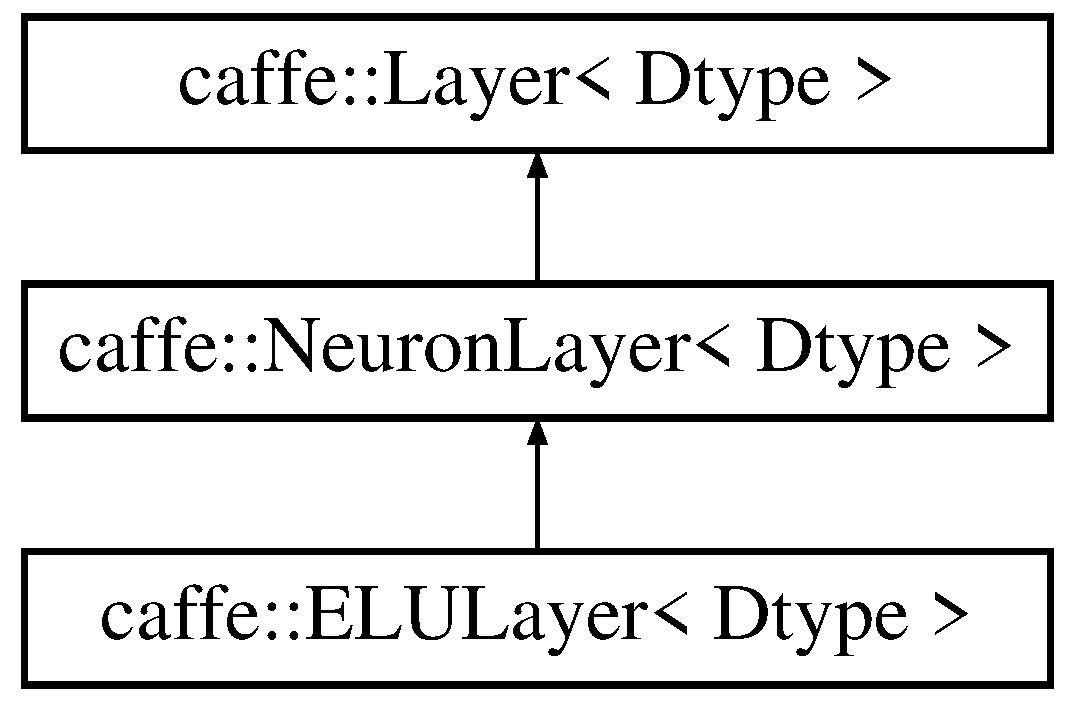
\includegraphics[height=3.000000cm]{classcaffe_1_1ELULayer}
\end{center}
\end{figure}
\subsection*{Public Member Functions}
\begin{DoxyCompactItemize}
\item 
\hyperlink{classcaffe_1_1ELULayer_af0b475c3d3b68f6daf7e2edcb7d5b97a}{E\+L\+U\+Layer} (const Layer\+Parameter \&param)
\item 
virtual const char $\ast$ \hyperlink{classcaffe_1_1ELULayer_a873d1abfe75142b44bea0507bef51c03}{type} () const \hypertarget{classcaffe_1_1ELULayer_a873d1abfe75142b44bea0507bef51c03}{}\label{classcaffe_1_1ELULayer_a873d1abfe75142b44bea0507bef51c03}

\begin{DoxyCompactList}\small\item\em Returns the layer type. \end{DoxyCompactList}\end{DoxyCompactItemize}
\subsection*{Protected Member Functions}
\begin{DoxyCompactItemize}
\item 
virtual void \hyperlink{classcaffe_1_1ELULayer_a2699f747f8702f7c640c4a275b34fa58}{Forward\+\_\+cpu} (const vector$<$ \hyperlink{classcaffe_1_1Blob}{Blob}$<$ Dtype $>$ $\ast$ $>$ \&bottom, const vector$<$ \hyperlink{classcaffe_1_1Blob}{Blob}$<$ Dtype $>$ $\ast$ $>$ \&top)
\item 
virtual void \hyperlink{classcaffe_1_1ELULayer_a603dd731816bb2be5b88bff94140e0bb}{Forward\+\_\+gpu} (const vector$<$ \hyperlink{classcaffe_1_1Blob}{Blob}$<$ Dtype $>$ $\ast$ $>$ \&bottom, const vector$<$ \hyperlink{classcaffe_1_1Blob}{Blob}$<$ Dtype $>$ $\ast$ $>$ \&top)\hypertarget{classcaffe_1_1ELULayer_a603dd731816bb2be5b88bff94140e0bb}{}\label{classcaffe_1_1ELULayer_a603dd731816bb2be5b88bff94140e0bb}

\begin{DoxyCompactList}\small\item\em Using the G\+PU device, compute the layer output. Fall back to \hyperlink{classcaffe_1_1ELULayer_a2699f747f8702f7c640c4a275b34fa58}{Forward\+\_\+cpu()} if unavailable. \end{DoxyCompactList}\item 
virtual void \hyperlink{classcaffe_1_1ELULayer_ae6ec837971800a3dce6d72a984cec0c6}{Backward\+\_\+cpu} (const vector$<$ \hyperlink{classcaffe_1_1Blob}{Blob}$<$ Dtype $>$ $\ast$ $>$ \&top, const vector$<$ bool $>$ \&propagate\+\_\+down, const vector$<$ \hyperlink{classcaffe_1_1Blob}{Blob}$<$ Dtype $>$ $\ast$ $>$ \&bottom)
\begin{DoxyCompactList}\small\item\em Computes the error gradient w.\+r.\+t. the E\+LU inputs. \end{DoxyCompactList}\item 
virtual void \hyperlink{classcaffe_1_1ELULayer_a0e45de15c2ae6cfeda87733730ab57de}{Backward\+\_\+gpu} (const vector$<$ \hyperlink{classcaffe_1_1Blob}{Blob}$<$ Dtype $>$ $\ast$ $>$ \&top, const vector$<$ bool $>$ \&propagate\+\_\+down, const vector$<$ \hyperlink{classcaffe_1_1Blob}{Blob}$<$ Dtype $>$ $\ast$ $>$ \&bottom)\hypertarget{classcaffe_1_1ELULayer_a0e45de15c2ae6cfeda87733730ab57de}{}\label{classcaffe_1_1ELULayer_a0e45de15c2ae6cfeda87733730ab57de}

\begin{DoxyCompactList}\small\item\em Using the G\+PU device, compute the gradients for any parameters and for the bottom blobs if propagate\+\_\+down is true. Fall back to \hyperlink{classcaffe_1_1ELULayer_ae6ec837971800a3dce6d72a984cec0c6}{Backward\+\_\+cpu()} if unavailable. \end{DoxyCompactList}\end{DoxyCompactItemize}
\subsection*{Additional Inherited Members}


\subsection{Detailed Description}
\subsubsection*{template$<$typename Dtype$>$\\*
class caffe\+::\+E\+L\+U\+Layer$<$ Dtype $>$}

Exponential Linear Unit non-\/linearity $ y = \left\{ \begin{array}{lr} x & \mathrm{if} \; x > 0 \\ \alpha (\exp(x)-1) & \mathrm{if} \; x \le 0 \end{array} \right. $. 

\subsection{Constructor \& Destructor Documentation}
\index{caffe\+::\+E\+L\+U\+Layer@{caffe\+::\+E\+L\+U\+Layer}!E\+L\+U\+Layer@{E\+L\+U\+Layer}}
\index{E\+L\+U\+Layer@{E\+L\+U\+Layer}!caffe\+::\+E\+L\+U\+Layer@{caffe\+::\+E\+L\+U\+Layer}}
\subsubsection[{\texorpdfstring{E\+L\+U\+Layer(const Layer\+Parameter \&param)}{ELULayer(const LayerParameter &param)}}]{\setlength{\rightskip}{0pt plus 5cm}template$<$typename Dtype $>$ {\bf caffe\+::\+E\+L\+U\+Layer}$<$ Dtype $>$\+::{\bf E\+L\+U\+Layer} (
\begin{DoxyParamCaption}
\item[{const Layer\+Parameter \&}]{param}
\end{DoxyParamCaption}
)\hspace{0.3cm}{\ttfamily [inline]}, {\ttfamily [explicit]}}\hypertarget{classcaffe_1_1ELULayer_af0b475c3d3b68f6daf7e2edcb7d5b97a}{}\label{classcaffe_1_1ELULayer_af0b475c3d3b68f6daf7e2edcb7d5b97a}

\begin{DoxyParams}{Parameters}
{\em param} & provides E\+L\+U\+Parameter elu\+\_\+param, with \hyperlink{classcaffe_1_1ELULayer}{E\+L\+U\+Layer} options\+:
\begin{DoxyItemize}
\item alpha ({\bfseries optional}, default 1). the value $ \alpha $ by which controls saturation for negative inputs. 
\end{DoxyItemize}\\
\hline
\end{DoxyParams}


\subsection{Member Function Documentation}
\index{caffe\+::\+E\+L\+U\+Layer@{caffe\+::\+E\+L\+U\+Layer}!Backward\+\_\+cpu@{Backward\+\_\+cpu}}
\index{Backward\+\_\+cpu@{Backward\+\_\+cpu}!caffe\+::\+E\+L\+U\+Layer@{caffe\+::\+E\+L\+U\+Layer}}
\subsubsection[{\texorpdfstring{Backward\+\_\+cpu(const vector$<$ Blob$<$ Dtype $>$ $\ast$ $>$ \&top, const vector$<$ bool $>$ \&propagate\+\_\+down, const vector$<$ Blob$<$ Dtype $>$ $\ast$ $>$ \&bottom)}{Backward_cpu(const vector< Blob< Dtype > * > &top, const vector< bool > &propagate_down, const vector< Blob< Dtype > * > &bottom)}}]{\setlength{\rightskip}{0pt plus 5cm}template$<$typename Dtype $>$ void {\bf caffe\+::\+E\+L\+U\+Layer}$<$ Dtype $>$\+::Backward\+\_\+cpu (
\begin{DoxyParamCaption}
\item[{const vector$<$ {\bf Blob}$<$ Dtype $>$ $\ast$ $>$ \&}]{top, }
\item[{const vector$<$ bool $>$ \&}]{propagate\+\_\+down, }
\item[{const vector$<$ {\bf Blob}$<$ Dtype $>$ $\ast$ $>$ \&}]{bottom}
\end{DoxyParamCaption}
)\hspace{0.3cm}{\ttfamily [protected]}, {\ttfamily [virtual]}}\hypertarget{classcaffe_1_1ELULayer_ae6ec837971800a3dce6d72a984cec0c6}{}\label{classcaffe_1_1ELULayer_ae6ec837971800a3dce6d72a984cec0c6}


Computes the error gradient w.\+r.\+t. the E\+LU inputs. 


\begin{DoxyParams}{Parameters}
{\em top} & output \hyperlink{classcaffe_1_1Blob}{Blob} vector (length 1), providing the error gradient with respect to the outputs
\begin{DoxyEnumerate}
\item $ (N \times C \times H \times W) $ containing error gradients $ \frac{\partial E}{\partial y} $ with respect to computed outputs $ y $ 
\end{DoxyEnumerate}\\
\hline
{\em propagate\+\_\+down} & see \hyperlink{classcaffe_1_1Layer_a53df1e081767e07bfb4c81657f4acd0a}{Layer\+::\+Backward}. \\
\hline
{\em bottom} & input \hyperlink{classcaffe_1_1Blob}{Blob} vector (length 1)
\begin{DoxyEnumerate}
\item $ (N \times C \times H \times W) $ the inputs $ x $; Backward fills their diff with gradients $ \frac{\partial E}{\partial x} = \left\{ \begin{array}{lr} 1 & \mathrm{if} \; x > 0 \\ y + \alpha & \mathrm{if} \; x \le 0 \end{array} \right. $ if propagate\+\_\+down\mbox{[}0\mbox{]}. 
\end{DoxyEnumerate}\\
\hline
\end{DoxyParams}


Implements \hyperlink{classcaffe_1_1Layer_a64d15855f882af4b82e83fa993c4e7c6}{caffe\+::\+Layer$<$ Dtype $>$}.

\index{caffe\+::\+E\+L\+U\+Layer@{caffe\+::\+E\+L\+U\+Layer}!Forward\+\_\+cpu@{Forward\+\_\+cpu}}
\index{Forward\+\_\+cpu@{Forward\+\_\+cpu}!caffe\+::\+E\+L\+U\+Layer@{caffe\+::\+E\+L\+U\+Layer}}
\subsubsection[{\texorpdfstring{Forward\+\_\+cpu(const vector$<$ Blob$<$ Dtype $>$ $\ast$ $>$ \&bottom, const vector$<$ Blob$<$ Dtype $>$ $\ast$ $>$ \&top)}{Forward_cpu(const vector< Blob< Dtype > * > &bottom, const vector< Blob< Dtype > * > &top)}}]{\setlength{\rightskip}{0pt plus 5cm}template$<$typename Dtype $>$ void {\bf caffe\+::\+E\+L\+U\+Layer}$<$ Dtype $>$\+::Forward\+\_\+cpu (
\begin{DoxyParamCaption}
\item[{const vector$<$ {\bf Blob}$<$ Dtype $>$ $\ast$ $>$ \&}]{bottom, }
\item[{const vector$<$ {\bf Blob}$<$ Dtype $>$ $\ast$ $>$ \&}]{top}
\end{DoxyParamCaption}
)\hspace{0.3cm}{\ttfamily [protected]}, {\ttfamily [virtual]}}\hypertarget{classcaffe_1_1ELULayer_a2699f747f8702f7c640c4a275b34fa58}{}\label{classcaffe_1_1ELULayer_a2699f747f8702f7c640c4a275b34fa58}

\begin{DoxyParams}{Parameters}
{\em bottom} & input \hyperlink{classcaffe_1_1Blob}{Blob} vector (length 1)
\begin{DoxyEnumerate}
\item $ (N \times C \times H \times W) $ the inputs $ x $ 
\end{DoxyEnumerate}\\
\hline
{\em top} & output \hyperlink{classcaffe_1_1Blob}{Blob} vector (length 1)
\begin{DoxyEnumerate}
\item $ (N \times C \times H \times W) $ the computed outputs $ y = \left\{ \begin{array}{lr} x & \mathrm{if} \; x > 0 \\ \alpha (\exp(x)-1) & \mathrm{if} \; x \le 0 \end{array} \right. $. 
\end{DoxyEnumerate}\\
\hline
\end{DoxyParams}


Implements \hyperlink{classcaffe_1_1Layer_add965883f75bbf90c7a06f960cda7a1a}{caffe\+::\+Layer$<$ Dtype $>$}.



The documentation for this class was generated from the following files\+:\begin{DoxyCompactItemize}
\item 
include/caffe/layers/elu\+\_\+layer.\+hpp\item 
src/caffe/layers/elu\+\_\+layer.\+cpp\end{DoxyCompactItemize}

\hypertarget{classcaffe_1_1EmbedLayer}{}\section{caffe\+:\+:Embed\+Layer$<$ Dtype $>$ Class Template Reference}
\label{classcaffe_1_1EmbedLayer}\index{caffe\+::\+Embed\+Layer$<$ Dtype $>$@{caffe\+::\+Embed\+Layer$<$ Dtype $>$}}


A layer for learning \char`\"{}embeddings\char`\"{} of one-\/hot vector input. Equivalent to an \hyperlink{classcaffe_1_1InnerProductLayer}{Inner\+Product\+Layer} with one-\/hot vectors as input, but for efficiency the input is the \char`\"{}hot\char`\"{} index of each column itself.  




{\ttfamily \#include $<$embed\+\_\+layer.\+hpp$>$}

Inheritance diagram for caffe\+:\+:Embed\+Layer$<$ Dtype $>$\+:\begin{figure}[H]
\begin{center}
\leavevmode
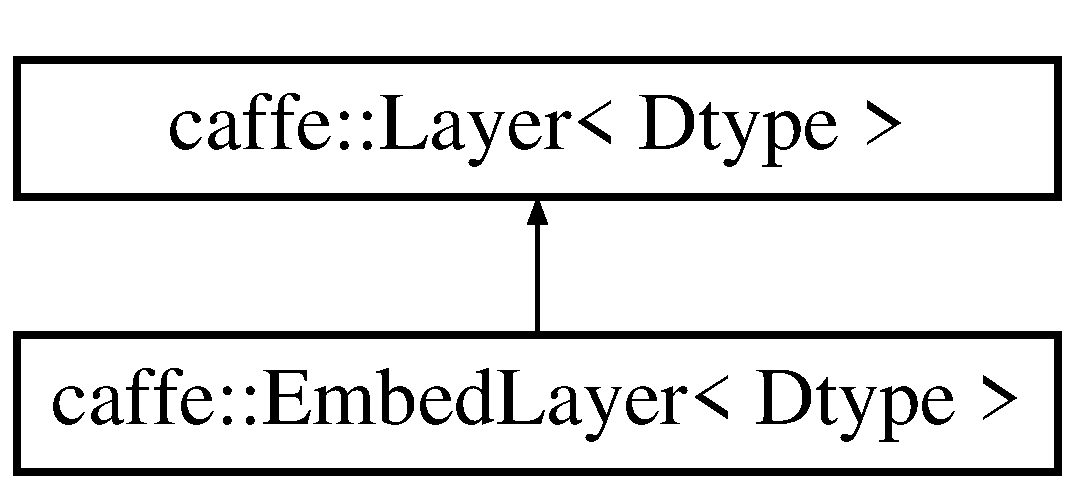
\includegraphics[height=2.000000cm]{classcaffe_1_1EmbedLayer}
\end{center}
\end{figure}
\subsection*{Public Member Functions}
\begin{DoxyCompactItemize}
\item 
{\bfseries Embed\+Layer} (const Layer\+Parameter \&param)\hypertarget{classcaffe_1_1EmbedLayer_afbf978848b6e28d3fd549d780f5b82ae}{}\label{classcaffe_1_1EmbedLayer_afbf978848b6e28d3fd549d780f5b82ae}

\item 
virtual void \hyperlink{classcaffe_1_1EmbedLayer_abd8a6ec0202709e3a1e06fb332332f4f}{Layer\+Set\+Up} (const vector$<$ \hyperlink{classcaffe_1_1Blob}{Blob}$<$ Dtype $>$ $\ast$ $>$ \&bottom, const vector$<$ \hyperlink{classcaffe_1_1Blob}{Blob}$<$ Dtype $>$ $\ast$ $>$ \&top)
\begin{DoxyCompactList}\small\item\em Does layer-\/specific setup\+: your layer should implement this function as well as Reshape. \end{DoxyCompactList}\item 
virtual void \hyperlink{classcaffe_1_1EmbedLayer_a46d98c49002ad119bd4e588bad859bc7}{Reshape} (const vector$<$ \hyperlink{classcaffe_1_1Blob}{Blob}$<$ Dtype $>$ $\ast$ $>$ \&bottom, const vector$<$ \hyperlink{classcaffe_1_1Blob}{Blob}$<$ Dtype $>$ $\ast$ $>$ \&top)
\begin{DoxyCompactList}\small\item\em Adjust the shapes of top blobs and internal buffers to accommodate the shapes of the bottom blobs. \end{DoxyCompactList}\item 
virtual const char $\ast$ \hyperlink{classcaffe_1_1EmbedLayer_ace6cb160fa74766b66a02f7d88d532f8}{type} () const \hypertarget{classcaffe_1_1EmbedLayer_ace6cb160fa74766b66a02f7d88d532f8}{}\label{classcaffe_1_1EmbedLayer_ace6cb160fa74766b66a02f7d88d532f8}

\begin{DoxyCompactList}\small\item\em Returns the layer type. \end{DoxyCompactList}\item 
virtual int \hyperlink{classcaffe_1_1EmbedLayer_ad32929e7b7b9f3467425065c1d037c07}{Exact\+Num\+Bottom\+Blobs} () const 
\begin{DoxyCompactList}\small\item\em Returns the exact number of bottom blobs required by the layer, or -\/1 if no exact number is required. \end{DoxyCompactList}\item 
virtual int \hyperlink{classcaffe_1_1EmbedLayer_a4555e4767b2ce8a32a23e5b1281f8a91}{Exact\+Num\+Top\+Blobs} () const 
\begin{DoxyCompactList}\small\item\em Returns the exact number of top blobs required by the layer, or -\/1 if no exact number is required. \end{DoxyCompactList}\end{DoxyCompactItemize}
\subsection*{Protected Member Functions}
\begin{DoxyCompactItemize}
\item 
virtual void \hyperlink{classcaffe_1_1EmbedLayer_a76b6e7470299ed7e3cad51061aee6450}{Forward\+\_\+cpu} (const vector$<$ \hyperlink{classcaffe_1_1Blob}{Blob}$<$ Dtype $>$ $\ast$ $>$ \&bottom, const vector$<$ \hyperlink{classcaffe_1_1Blob}{Blob}$<$ Dtype $>$ $\ast$ $>$ \&top)\hypertarget{classcaffe_1_1EmbedLayer_a76b6e7470299ed7e3cad51061aee6450}{}\label{classcaffe_1_1EmbedLayer_a76b6e7470299ed7e3cad51061aee6450}

\begin{DoxyCompactList}\small\item\em Using the C\+PU device, compute the layer output. \end{DoxyCompactList}\item 
virtual void \hyperlink{classcaffe_1_1EmbedLayer_add9d5ee768c226f93130ccce47bd0023}{Forward\+\_\+gpu} (const vector$<$ \hyperlink{classcaffe_1_1Blob}{Blob}$<$ Dtype $>$ $\ast$ $>$ \&bottom, const vector$<$ \hyperlink{classcaffe_1_1Blob}{Blob}$<$ Dtype $>$ $\ast$ $>$ \&top)\hypertarget{classcaffe_1_1EmbedLayer_add9d5ee768c226f93130ccce47bd0023}{}\label{classcaffe_1_1EmbedLayer_add9d5ee768c226f93130ccce47bd0023}

\begin{DoxyCompactList}\small\item\em Using the G\+PU device, compute the layer output. Fall back to \hyperlink{classcaffe_1_1EmbedLayer_a76b6e7470299ed7e3cad51061aee6450}{Forward\+\_\+cpu()} if unavailable. \end{DoxyCompactList}\item 
virtual void \hyperlink{classcaffe_1_1EmbedLayer_a863ed3e35d22a1b7b64c05b3dcafc218}{Backward\+\_\+cpu} (const vector$<$ \hyperlink{classcaffe_1_1Blob}{Blob}$<$ Dtype $>$ $\ast$ $>$ \&top, const vector$<$ bool $>$ \&propagate\+\_\+down, const vector$<$ \hyperlink{classcaffe_1_1Blob}{Blob}$<$ Dtype $>$ $\ast$ $>$ \&bottom)\hypertarget{classcaffe_1_1EmbedLayer_a863ed3e35d22a1b7b64c05b3dcafc218}{}\label{classcaffe_1_1EmbedLayer_a863ed3e35d22a1b7b64c05b3dcafc218}

\begin{DoxyCompactList}\small\item\em Using the C\+PU device, compute the gradients for any parameters and for the bottom blobs if propagate\+\_\+down is true. \end{DoxyCompactList}\item 
virtual void \hyperlink{classcaffe_1_1EmbedLayer_a30400163dd2be3ab4c53d4bcd951a580}{Backward\+\_\+gpu} (const vector$<$ \hyperlink{classcaffe_1_1Blob}{Blob}$<$ Dtype $>$ $\ast$ $>$ \&top, const vector$<$ bool $>$ \&propagate\+\_\+down, const vector$<$ \hyperlink{classcaffe_1_1Blob}{Blob}$<$ Dtype $>$ $\ast$ $>$ \&bottom)\hypertarget{classcaffe_1_1EmbedLayer_a30400163dd2be3ab4c53d4bcd951a580}{}\label{classcaffe_1_1EmbedLayer_a30400163dd2be3ab4c53d4bcd951a580}

\begin{DoxyCompactList}\small\item\em Using the G\+PU device, compute the gradients for any parameters and for the bottom blobs if propagate\+\_\+down is true. Fall back to \hyperlink{classcaffe_1_1EmbedLayer_a863ed3e35d22a1b7b64c05b3dcafc218}{Backward\+\_\+cpu()} if unavailable. \end{DoxyCompactList}\end{DoxyCompactItemize}
\subsection*{Protected Attributes}
\begin{DoxyCompactItemize}
\item 
int {\bfseries M\+\_\+}\hypertarget{classcaffe_1_1EmbedLayer_ab141ec84d4a4617c69534594f32de458}{}\label{classcaffe_1_1EmbedLayer_ab141ec84d4a4617c69534594f32de458}

\item 
int {\bfseries K\+\_\+}\hypertarget{classcaffe_1_1EmbedLayer_a4c3ea441f384c996a22bf5f5927119a5}{}\label{classcaffe_1_1EmbedLayer_a4c3ea441f384c996a22bf5f5927119a5}

\item 
int {\bfseries N\+\_\+}\hypertarget{classcaffe_1_1EmbedLayer_a47e98f5f2b174d63e5563391d27e61c7}{}\label{classcaffe_1_1EmbedLayer_a47e98f5f2b174d63e5563391d27e61c7}

\item 
bool {\bfseries bias\+\_\+term\+\_\+}\hypertarget{classcaffe_1_1EmbedLayer_aa961db47dca56c819cf9b6c185227cbd}{}\label{classcaffe_1_1EmbedLayer_aa961db47dca56c819cf9b6c185227cbd}

\item 
\hyperlink{classcaffe_1_1Blob}{Blob}$<$ Dtype $>$ {\bfseries bias\+\_\+multiplier\+\_\+}\hypertarget{classcaffe_1_1EmbedLayer_a8b7542af1502f96d4d811db337bb7727}{}\label{classcaffe_1_1EmbedLayer_a8b7542af1502f96d4d811db337bb7727}

\end{DoxyCompactItemize}


\subsection{Detailed Description}
\subsubsection*{template$<$typename Dtype$>$\\*
class caffe\+::\+Embed\+Layer$<$ Dtype $>$}

A layer for learning \char`\"{}embeddings\char`\"{} of one-\/hot vector input. Equivalent to an \hyperlink{classcaffe_1_1InnerProductLayer}{Inner\+Product\+Layer} with one-\/hot vectors as input, but for efficiency the input is the \char`\"{}hot\char`\"{} index of each column itself. 

T\+O\+D\+O(dox)\+: thorough documentation for Forward, Backward, and proto params. 

\subsection{Member Function Documentation}
\index{caffe\+::\+Embed\+Layer@{caffe\+::\+Embed\+Layer}!Exact\+Num\+Bottom\+Blobs@{Exact\+Num\+Bottom\+Blobs}}
\index{Exact\+Num\+Bottom\+Blobs@{Exact\+Num\+Bottom\+Blobs}!caffe\+::\+Embed\+Layer@{caffe\+::\+Embed\+Layer}}
\subsubsection[{\texorpdfstring{Exact\+Num\+Bottom\+Blobs() const }{ExactNumBottomBlobs() const }}]{\setlength{\rightskip}{0pt plus 5cm}template$<$typename Dtype $>$ virtual int {\bf caffe\+::\+Embed\+Layer}$<$ Dtype $>$\+::Exact\+Num\+Bottom\+Blobs (
\begin{DoxyParamCaption}
{}
\end{DoxyParamCaption}
) const\hspace{0.3cm}{\ttfamily [inline]}, {\ttfamily [virtual]}}\hypertarget{classcaffe_1_1EmbedLayer_ad32929e7b7b9f3467425065c1d037c07}{}\label{classcaffe_1_1EmbedLayer_ad32929e7b7b9f3467425065c1d037c07}


Returns the exact number of bottom blobs required by the layer, or -\/1 if no exact number is required. 

This method should be overridden to return a non-\/negative value if your layer expects some exact number of bottom blobs. 

Reimplemented from \hyperlink{classcaffe_1_1Layer_a45c7a7943a8a6735ac433c9be11e0240}{caffe\+::\+Layer$<$ Dtype $>$}.

\index{caffe\+::\+Embed\+Layer@{caffe\+::\+Embed\+Layer}!Exact\+Num\+Top\+Blobs@{Exact\+Num\+Top\+Blobs}}
\index{Exact\+Num\+Top\+Blobs@{Exact\+Num\+Top\+Blobs}!caffe\+::\+Embed\+Layer@{caffe\+::\+Embed\+Layer}}
\subsubsection[{\texorpdfstring{Exact\+Num\+Top\+Blobs() const }{ExactNumTopBlobs() const }}]{\setlength{\rightskip}{0pt plus 5cm}template$<$typename Dtype $>$ virtual int {\bf caffe\+::\+Embed\+Layer}$<$ Dtype $>$\+::Exact\+Num\+Top\+Blobs (
\begin{DoxyParamCaption}
{}
\end{DoxyParamCaption}
) const\hspace{0.3cm}{\ttfamily [inline]}, {\ttfamily [virtual]}}\hypertarget{classcaffe_1_1EmbedLayer_a4555e4767b2ce8a32a23e5b1281f8a91}{}\label{classcaffe_1_1EmbedLayer_a4555e4767b2ce8a32a23e5b1281f8a91}


Returns the exact number of top blobs required by the layer, or -\/1 if no exact number is required. 

This method should be overridden to return a non-\/negative value if your layer expects some exact number of top blobs. 

Reimplemented from \hyperlink{classcaffe_1_1Layer_aa3c99ed707e8db683a3043412e151af8}{caffe\+::\+Layer$<$ Dtype $>$}.

\index{caffe\+::\+Embed\+Layer@{caffe\+::\+Embed\+Layer}!Layer\+Set\+Up@{Layer\+Set\+Up}}
\index{Layer\+Set\+Up@{Layer\+Set\+Up}!caffe\+::\+Embed\+Layer@{caffe\+::\+Embed\+Layer}}
\subsubsection[{\texorpdfstring{Layer\+Set\+Up(const vector$<$ Blob$<$ Dtype $>$ $\ast$ $>$ \&bottom, const vector$<$ Blob$<$ Dtype $>$ $\ast$ $>$ \&top)}{LayerSetUp(const vector< Blob< Dtype > * > &bottom, const vector< Blob< Dtype > * > &top)}}]{\setlength{\rightskip}{0pt plus 5cm}template$<$typename Dtype $>$ void {\bf caffe\+::\+Embed\+Layer}$<$ Dtype $>$\+::Layer\+Set\+Up (
\begin{DoxyParamCaption}
\item[{const vector$<$ {\bf Blob}$<$ Dtype $>$ $\ast$ $>$ \&}]{bottom, }
\item[{const vector$<$ {\bf Blob}$<$ Dtype $>$ $\ast$ $>$ \&}]{top}
\end{DoxyParamCaption}
)\hspace{0.3cm}{\ttfamily [virtual]}}\hypertarget{classcaffe_1_1EmbedLayer_abd8a6ec0202709e3a1e06fb332332f4f}{}\label{classcaffe_1_1EmbedLayer_abd8a6ec0202709e3a1e06fb332332f4f}


Does layer-\/specific setup\+: your layer should implement this function as well as Reshape. 


\begin{DoxyParams}{Parameters}
{\em bottom} & the preshaped input blobs, whose data fields store the input data for this layer \\
\hline
{\em top} & the allocated but unshaped output blobs\\
\hline
\end{DoxyParams}
This method should do one-\/time layer specific setup. This includes reading and processing relevent parameters from the {\ttfamily layer\+\_\+param\+\_\+}. Setting up the shapes of top blobs and internal buffers should be done in {\ttfamily Reshape}, which will be called before the forward pass to adjust the top blob sizes. 

Reimplemented from \hyperlink{classcaffe_1_1Layer_a38dc2488bf319b8de5a7ac84e0045393}{caffe\+::\+Layer$<$ Dtype $>$}.

\index{caffe\+::\+Embed\+Layer@{caffe\+::\+Embed\+Layer}!Reshape@{Reshape}}
\index{Reshape@{Reshape}!caffe\+::\+Embed\+Layer@{caffe\+::\+Embed\+Layer}}
\subsubsection[{\texorpdfstring{Reshape(const vector$<$ Blob$<$ Dtype $>$ $\ast$ $>$ \&bottom, const vector$<$ Blob$<$ Dtype $>$ $\ast$ $>$ \&top)}{Reshape(const vector< Blob< Dtype > * > &bottom, const vector< Blob< Dtype > * > &top)}}]{\setlength{\rightskip}{0pt plus 5cm}template$<$typename Dtype $>$ void {\bf caffe\+::\+Embed\+Layer}$<$ Dtype $>$\+::Reshape (
\begin{DoxyParamCaption}
\item[{const vector$<$ {\bf Blob}$<$ Dtype $>$ $\ast$ $>$ \&}]{bottom, }
\item[{const vector$<$ {\bf Blob}$<$ Dtype $>$ $\ast$ $>$ \&}]{top}
\end{DoxyParamCaption}
)\hspace{0.3cm}{\ttfamily [virtual]}}\hypertarget{classcaffe_1_1EmbedLayer_a46d98c49002ad119bd4e588bad859bc7}{}\label{classcaffe_1_1EmbedLayer_a46d98c49002ad119bd4e588bad859bc7}


Adjust the shapes of top blobs and internal buffers to accommodate the shapes of the bottom blobs. 


\begin{DoxyParams}{Parameters}
{\em bottom} & the input blobs, with the requested input shapes \\
\hline
{\em top} & the top blobs, which should be reshaped as needed\\
\hline
\end{DoxyParams}
This method should reshape top blobs as needed according to the shapes of the bottom (input) blobs, as well as reshaping any internal buffers and making any other necessary adjustments so that the layer can accommodate the bottom blobs. 

Implements \hyperlink{classcaffe_1_1Layer_ad9d391b972c769c0ebee34ca6d1c973e}{caffe\+::\+Layer$<$ Dtype $>$}.



The documentation for this class was generated from the following files\+:\begin{DoxyCompactItemize}
\item 
include/caffe/layers/embed\+\_\+layer.\+hpp\item 
src/caffe/layers/embed\+\_\+layer.\+cpp\end{DoxyCompactItemize}

\hypertarget{classcaffe_1_1EuclideanLossLayer}{}\section{caffe\+:\+:Euclidean\+Loss\+Layer$<$ Dtype $>$ Class Template Reference}
\label{classcaffe_1_1EuclideanLossLayer}\index{caffe\+::\+Euclidean\+Loss\+Layer$<$ Dtype $>$@{caffe\+::\+Euclidean\+Loss\+Layer$<$ Dtype $>$}}


Computes the Euclidean (L2) loss $ E = \frac{1}{2N} \sum\limits_{n=1}^N \left| \left| \hat{y}_n - y_n \right| \right|_2^2 $ for real-\/valued regression tasks.  




{\ttfamily \#include $<$euclidean\+\_\+loss\+\_\+layer.\+hpp$>$}

Inheritance diagram for caffe\+:\+:Euclidean\+Loss\+Layer$<$ Dtype $>$\+:\begin{figure}[H]
\begin{center}
\leavevmode
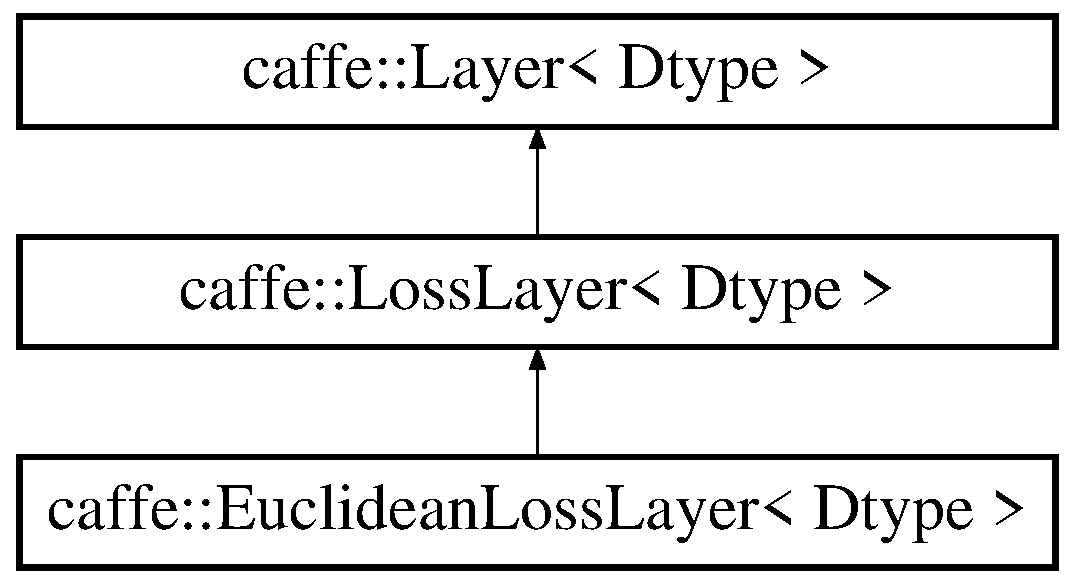
\includegraphics[height=3.000000cm]{classcaffe_1_1EuclideanLossLayer}
\end{center}
\end{figure}
\subsection*{Public Member Functions}
\begin{DoxyCompactItemize}
\item 
{\bfseries Euclidean\+Loss\+Layer} (const Layer\+Parameter \&param)\hypertarget{classcaffe_1_1EuclideanLossLayer_aea3a6d5454ee1a0db7cdb6c59bcfc5c8}{}\label{classcaffe_1_1EuclideanLossLayer_aea3a6d5454ee1a0db7cdb6c59bcfc5c8}

\item 
virtual void \hyperlink{classcaffe_1_1EuclideanLossLayer_a4d2df2fad6e3d04ed24df9fe6460c683}{Reshape} (const vector$<$ \hyperlink{classcaffe_1_1Blob}{Blob}$<$ Dtype $>$ $\ast$ $>$ \&bottom, const vector$<$ \hyperlink{classcaffe_1_1Blob}{Blob}$<$ Dtype $>$ $\ast$ $>$ \&top)
\begin{DoxyCompactList}\small\item\em Adjust the shapes of top blobs and internal buffers to accommodate the shapes of the bottom blobs. \end{DoxyCompactList}\item 
virtual const char $\ast$ \hyperlink{classcaffe_1_1EuclideanLossLayer_af7c7836f04594b7564b2d740ccaed559}{type} () const \hypertarget{classcaffe_1_1EuclideanLossLayer_af7c7836f04594b7564b2d740ccaed559}{}\label{classcaffe_1_1EuclideanLossLayer_af7c7836f04594b7564b2d740ccaed559}

\begin{DoxyCompactList}\small\item\em Returns the layer type. \end{DoxyCompactList}\item 
virtual bool \hyperlink{classcaffe_1_1EuclideanLossLayer_a3c954fd7c15596fd2f59e0f79601905c}{Allow\+Force\+Backward} (const int bottom\+\_\+index) const 
\end{DoxyCompactItemize}
\subsection*{Protected Member Functions}
\begin{DoxyCompactItemize}
\item 
virtual void \hyperlink{classcaffe_1_1EuclideanLossLayer_aa642f3d938b4e1d0c8b240c68ba8a856}{Forward\+\_\+cpu} (const vector$<$ \hyperlink{classcaffe_1_1Blob}{Blob}$<$ Dtype $>$ $\ast$ $>$ \&bottom, const vector$<$ \hyperlink{classcaffe_1_1Blob}{Blob}$<$ Dtype $>$ $\ast$ $>$ \&top)
\begin{DoxyCompactList}\small\item\em Computes the Euclidean (L2) loss $ E = \frac{1}{2N} \sum\limits_{n=1}^N \left| \left| \hat{y}_n - y_n \right| \right|_2^2 $ for real-\/valued regression tasks. \end{DoxyCompactList}\item 
virtual void \hyperlink{classcaffe_1_1EuclideanLossLayer_a0eddd3fca6ec788b61bc55960cbce68a}{Forward\+\_\+gpu} (const vector$<$ \hyperlink{classcaffe_1_1Blob}{Blob}$<$ Dtype $>$ $\ast$ $>$ \&bottom, const vector$<$ \hyperlink{classcaffe_1_1Blob}{Blob}$<$ Dtype $>$ $\ast$ $>$ \&top)\hypertarget{classcaffe_1_1EuclideanLossLayer_a0eddd3fca6ec788b61bc55960cbce68a}{}\label{classcaffe_1_1EuclideanLossLayer_a0eddd3fca6ec788b61bc55960cbce68a}

\begin{DoxyCompactList}\small\item\em Using the G\+PU device, compute the layer output. Fall back to \hyperlink{classcaffe_1_1EuclideanLossLayer_aa642f3d938b4e1d0c8b240c68ba8a856}{Forward\+\_\+cpu()} if unavailable. \end{DoxyCompactList}\item 
virtual void \hyperlink{classcaffe_1_1EuclideanLossLayer_afc83c3980206b9c24b5985819c13475c}{Backward\+\_\+cpu} (const vector$<$ \hyperlink{classcaffe_1_1Blob}{Blob}$<$ Dtype $>$ $\ast$ $>$ \&top, const vector$<$ bool $>$ \&propagate\+\_\+down, const vector$<$ \hyperlink{classcaffe_1_1Blob}{Blob}$<$ Dtype $>$ $\ast$ $>$ \&bottom)
\begin{DoxyCompactList}\small\item\em Computes the Euclidean error gradient w.\+r.\+t. the inputs. \end{DoxyCompactList}\item 
virtual void \hyperlink{classcaffe_1_1EuclideanLossLayer_a2a7972df719c3a49a7308e78927fc024}{Backward\+\_\+gpu} (const vector$<$ \hyperlink{classcaffe_1_1Blob}{Blob}$<$ Dtype $>$ $\ast$ $>$ \&top, const vector$<$ bool $>$ \&propagate\+\_\+down, const vector$<$ \hyperlink{classcaffe_1_1Blob}{Blob}$<$ Dtype $>$ $\ast$ $>$ \&bottom)\hypertarget{classcaffe_1_1EuclideanLossLayer_a2a7972df719c3a49a7308e78927fc024}{}\label{classcaffe_1_1EuclideanLossLayer_a2a7972df719c3a49a7308e78927fc024}

\begin{DoxyCompactList}\small\item\em Using the G\+PU device, compute the gradients for any parameters and for the bottom blobs if propagate\+\_\+down is true. Fall back to \hyperlink{classcaffe_1_1EuclideanLossLayer_afc83c3980206b9c24b5985819c13475c}{Backward\+\_\+cpu()} if unavailable. \end{DoxyCompactList}\end{DoxyCompactItemize}
\subsection*{Protected Attributes}
\begin{DoxyCompactItemize}
\item 
\hyperlink{classcaffe_1_1Blob}{Blob}$<$ Dtype $>$ {\bfseries diff\+\_\+}\hypertarget{classcaffe_1_1EuclideanLossLayer_a47ec68365879c820f9e18e456f93376a}{}\label{classcaffe_1_1EuclideanLossLayer_a47ec68365879c820f9e18e456f93376a}

\end{DoxyCompactItemize}


\subsection{Detailed Description}
\subsubsection*{template$<$typename Dtype$>$\\*
class caffe\+::\+Euclidean\+Loss\+Layer$<$ Dtype $>$}

Computes the Euclidean (L2) loss $ E = \frac{1}{2N} \sum\limits_{n=1}^N \left| \left| \hat{y}_n - y_n \right| \right|_2^2 $ for real-\/valued regression tasks. 


\begin{DoxyParams}{Parameters}
{\em bottom} & input \hyperlink{classcaffe_1_1Blob}{Blob} vector (length 2)
\begin{DoxyEnumerate}
\item $ (N \times C \times H \times W) $ the predictions $ \hat{y} \in [-\infty, +\infty]$
\item $ (N \times C \times H \times W) $ the targets $ y \in [-\infty, +\infty]$ 
\end{DoxyEnumerate}\\
\hline
{\em top} & output \hyperlink{classcaffe_1_1Blob}{Blob} vector (length 1)
\begin{DoxyEnumerate}
\item $ (1 \times 1 \times 1 \times 1) $ the computed Euclidean loss\+: $ E = \frac{1}{2n} \sum\limits_{n=1}^N \left| \left| \hat{y}_n - y_n \right| \right|_2^2 $
\end{DoxyEnumerate}\\
\hline
\end{DoxyParams}
This can be used for least-\/squares regression tasks. An \hyperlink{classcaffe_1_1InnerProductLayer}{Inner\+Product\+Layer} input to a \hyperlink{classcaffe_1_1EuclideanLossLayer}{Euclidean\+Loss\+Layer} exactly formulates a linear least squares regression problem. With non-\/zero weight decay the problem becomes one of ridge regression -- see src/caffe/test/test\+\_\+gradient\+\_\+based\+\_\+solver.\+cpp for a concrete example wherein we check that the gradients computed for a \hyperlink{classcaffe_1_1Net}{Net} with exactly this structure match hand-\/computed gradient formulas for ridge regression.

(Note\+: \hyperlink{classcaffe_1_1Caffe}{Caffe}, and S\+GD in general, is certainly {\bfseries not} the best way to solve linear least squares problems! We use it only as an instructive example.) 

\subsection{Member Function Documentation}
\index{caffe\+::\+Euclidean\+Loss\+Layer@{caffe\+::\+Euclidean\+Loss\+Layer}!Allow\+Force\+Backward@{Allow\+Force\+Backward}}
\index{Allow\+Force\+Backward@{Allow\+Force\+Backward}!caffe\+::\+Euclidean\+Loss\+Layer@{caffe\+::\+Euclidean\+Loss\+Layer}}
\subsubsection[{\texorpdfstring{Allow\+Force\+Backward(const int bottom\+\_\+index) const }{AllowForceBackward(const int bottom_index) const }}]{\setlength{\rightskip}{0pt plus 5cm}template$<$typename Dtype $>$ virtual bool {\bf caffe\+::\+Euclidean\+Loss\+Layer}$<$ Dtype $>$\+::Allow\+Force\+Backward (
\begin{DoxyParamCaption}
\item[{const int}]{bottom\+\_\+index}
\end{DoxyParamCaption}
) const\hspace{0.3cm}{\ttfamily [inline]}, {\ttfamily [virtual]}}\hypertarget{classcaffe_1_1EuclideanLossLayer_a3c954fd7c15596fd2f59e0f79601905c}{}\label{classcaffe_1_1EuclideanLossLayer_a3c954fd7c15596fd2f59e0f79601905c}
Unlike most loss layers, in the \hyperlink{classcaffe_1_1EuclideanLossLayer}{Euclidean\+Loss\+Layer} we can backpropagate to both inputs -- override to return true and always allow force\+\_\+backward. 

Reimplemented from \hyperlink{classcaffe_1_1LossLayer_ad02fe695b06451ac8e6f21db0cba1dad}{caffe\+::\+Loss\+Layer$<$ Dtype $>$}.

\index{caffe\+::\+Euclidean\+Loss\+Layer@{caffe\+::\+Euclidean\+Loss\+Layer}!Backward\+\_\+cpu@{Backward\+\_\+cpu}}
\index{Backward\+\_\+cpu@{Backward\+\_\+cpu}!caffe\+::\+Euclidean\+Loss\+Layer@{caffe\+::\+Euclidean\+Loss\+Layer}}
\subsubsection[{\texorpdfstring{Backward\+\_\+cpu(const vector$<$ Blob$<$ Dtype $>$ $\ast$ $>$ \&top, const vector$<$ bool $>$ \&propagate\+\_\+down, const vector$<$ Blob$<$ Dtype $>$ $\ast$ $>$ \&bottom)}{Backward_cpu(const vector< Blob< Dtype > * > &top, const vector< bool > &propagate_down, const vector< Blob< Dtype > * > &bottom)}}]{\setlength{\rightskip}{0pt plus 5cm}template$<$typename Dtype $>$ void {\bf caffe\+::\+Euclidean\+Loss\+Layer}$<$ Dtype $>$\+::Backward\+\_\+cpu (
\begin{DoxyParamCaption}
\item[{const vector$<$ {\bf Blob}$<$ Dtype $>$ $\ast$ $>$ \&}]{top, }
\item[{const vector$<$ bool $>$ \&}]{propagate\+\_\+down, }
\item[{const vector$<$ {\bf Blob}$<$ Dtype $>$ $\ast$ $>$ \&}]{bottom}
\end{DoxyParamCaption}
)\hspace{0.3cm}{\ttfamily [protected]}, {\ttfamily [virtual]}}\hypertarget{classcaffe_1_1EuclideanLossLayer_afc83c3980206b9c24b5985819c13475c}{}\label{classcaffe_1_1EuclideanLossLayer_afc83c3980206b9c24b5985819c13475c}


Computes the Euclidean error gradient w.\+r.\+t. the inputs. 

Unlike other children of \hyperlink{classcaffe_1_1LossLayer}{Loss\+Layer}, \hyperlink{classcaffe_1_1EuclideanLossLayer}{Euclidean\+Loss\+Layer} {\bfseries can} compute gradients with respect to the label inputs bottom\mbox{[}1\mbox{]} (but still only will if propagate\+\_\+down\mbox{[}1\mbox{]} is set, due to being produced by learnable parameters or if force\+\_\+backward is set). In fact, this layer is \char`\"{}commutative\char`\"{} -- the result is the same regardless of the order of the two bottoms.


\begin{DoxyParams}{Parameters}
{\em top} & output \hyperlink{classcaffe_1_1Blob}{Blob} vector (length 1), providing the error gradient with respect to the outputs
\begin{DoxyEnumerate}
\item $ (1 \times 1 \times 1 \times 1) $ This \hyperlink{classcaffe_1_1Blob}{Blob}\textquotesingle{}s diff will simply contain the loss\+\_\+weight$\ast$ $ \lambda $, as $ \lambda $ is the coefficient of this layer\textquotesingle{}s output $\ell_i$ in the overall \hyperlink{classcaffe_1_1Net}{Net} loss $ E = \lambda_i \ell_i + \mbox{other loss terms}$; hence $ \frac{\partial E}{\partial \ell_i} = \lambda_i $. ($\ast$\+Assuming that this top \hyperlink{classcaffe_1_1Blob}{Blob} is not used as a bottom (input) by any other layer of the \hyperlink{classcaffe_1_1Net}{Net}.) 
\end{DoxyEnumerate}\\
\hline
{\em propagate\+\_\+down} & see \hyperlink{classcaffe_1_1Layer_a53df1e081767e07bfb4c81657f4acd0a}{Layer\+::\+Backward}. \\
\hline
{\em bottom} & input \hyperlink{classcaffe_1_1Blob}{Blob} vector (length 2)
\begin{DoxyEnumerate}
\item $ (N \times C \times H \times W) $ the predictions $\hat{y}$; Backward fills their diff with gradients $ \frac{\partial E}{\partial \hat{y}} = \frac{1}{n} \sum\limits_{n=1}^N (\hat{y}_n - y_n) $ if propagate\+\_\+down\mbox{[}0\mbox{]}
\item $ (N \times C \times H \times W) $ the targets $y$; Backward fills their diff with gradients $ \frac{\partial E}{\partial y} = \frac{1}{n} \sum\limits_{n=1}^N (y_n - \hat{y}_n) $ if propagate\+\_\+down\mbox{[}1\mbox{]} 
\end{DoxyEnumerate}\\
\hline
\end{DoxyParams}


Implements \hyperlink{classcaffe_1_1Layer_a64d15855f882af4b82e83fa993c4e7c6}{caffe\+::\+Layer$<$ Dtype $>$}.

\index{caffe\+::\+Euclidean\+Loss\+Layer@{caffe\+::\+Euclidean\+Loss\+Layer}!Forward\+\_\+cpu@{Forward\+\_\+cpu}}
\index{Forward\+\_\+cpu@{Forward\+\_\+cpu}!caffe\+::\+Euclidean\+Loss\+Layer@{caffe\+::\+Euclidean\+Loss\+Layer}}
\subsubsection[{\texorpdfstring{Forward\+\_\+cpu(const vector$<$ Blob$<$ Dtype $>$ $\ast$ $>$ \&bottom, const vector$<$ Blob$<$ Dtype $>$ $\ast$ $>$ \&top)}{Forward_cpu(const vector< Blob< Dtype > * > &bottom, const vector< Blob< Dtype > * > &top)}}]{\setlength{\rightskip}{0pt plus 5cm}template$<$typename Dtype $>$ void {\bf caffe\+::\+Euclidean\+Loss\+Layer}$<$ Dtype $>$\+::Forward\+\_\+cpu (
\begin{DoxyParamCaption}
\item[{const vector$<$ {\bf Blob}$<$ Dtype $>$ $\ast$ $>$ \&}]{bottom, }
\item[{const vector$<$ {\bf Blob}$<$ Dtype $>$ $\ast$ $>$ \&}]{top}
\end{DoxyParamCaption}
)\hspace{0.3cm}{\ttfamily [protected]}, {\ttfamily [virtual]}}\hypertarget{classcaffe_1_1EuclideanLossLayer_aa642f3d938b4e1d0c8b240c68ba8a856}{}\label{classcaffe_1_1EuclideanLossLayer_aa642f3d938b4e1d0c8b240c68ba8a856}


Computes the Euclidean (L2) loss $ E = \frac{1}{2N} \sum\limits_{n=1}^N \left| \left| \hat{y}_n - y_n \right| \right|_2^2 $ for real-\/valued regression tasks. 


\begin{DoxyParams}{Parameters}
{\em bottom} & input \hyperlink{classcaffe_1_1Blob}{Blob} vector (length 2)
\begin{DoxyEnumerate}
\item $ (N \times C \times H \times W) $ the predictions $ \hat{y} \in [-\infty, +\infty]$
\item $ (N \times C \times H \times W) $ the targets $ y \in [-\infty, +\infty]$ 
\end{DoxyEnumerate}\\
\hline
{\em top} & output \hyperlink{classcaffe_1_1Blob}{Blob} vector (length 1)
\begin{DoxyEnumerate}
\item $ (1 \times 1 \times 1 \times 1) $ the computed Euclidean loss\+: $ E = \frac{1}{2n} \sum\limits_{n=1}^N \left| \left| \hat{y}_n - y_n \right| \right|_2^2 $
\end{DoxyEnumerate}\\
\hline
\end{DoxyParams}
This can be used for least-\/squares regression tasks. An \hyperlink{classcaffe_1_1InnerProductLayer}{Inner\+Product\+Layer} input to a \hyperlink{classcaffe_1_1EuclideanLossLayer}{Euclidean\+Loss\+Layer} exactly formulates a linear least squares regression problem. With non-\/zero weight decay the problem becomes one of ridge regression -- see src/caffe/test/test\+\_\+gradient\+\_\+based\+\_\+solver.\+cpp for a concrete example wherein we check that the gradients computed for a \hyperlink{classcaffe_1_1Net}{Net} with exactly this structure match hand-\/computed gradient formulas for ridge regression.

(Note\+: \hyperlink{classcaffe_1_1Caffe}{Caffe}, and S\+GD in general, is certainly {\bfseries not} the best way to solve linear least squares problems! We use it only as an instructive example.) 

Implements \hyperlink{classcaffe_1_1Layer_add965883f75bbf90c7a06f960cda7a1a}{caffe\+::\+Layer$<$ Dtype $>$}.

\index{caffe\+::\+Euclidean\+Loss\+Layer@{caffe\+::\+Euclidean\+Loss\+Layer}!Reshape@{Reshape}}
\index{Reshape@{Reshape}!caffe\+::\+Euclidean\+Loss\+Layer@{caffe\+::\+Euclidean\+Loss\+Layer}}
\subsubsection[{\texorpdfstring{Reshape(const vector$<$ Blob$<$ Dtype $>$ $\ast$ $>$ \&bottom, const vector$<$ Blob$<$ Dtype $>$ $\ast$ $>$ \&top)}{Reshape(const vector< Blob< Dtype > * > &bottom, const vector< Blob< Dtype > * > &top)}}]{\setlength{\rightskip}{0pt plus 5cm}template$<$typename Dtype $>$ void {\bf caffe\+::\+Euclidean\+Loss\+Layer}$<$ Dtype $>$\+::Reshape (
\begin{DoxyParamCaption}
\item[{const vector$<$ {\bf Blob}$<$ Dtype $>$ $\ast$ $>$ \&}]{bottom, }
\item[{const vector$<$ {\bf Blob}$<$ Dtype $>$ $\ast$ $>$ \&}]{top}
\end{DoxyParamCaption}
)\hspace{0.3cm}{\ttfamily [virtual]}}\hypertarget{classcaffe_1_1EuclideanLossLayer_a4d2df2fad6e3d04ed24df9fe6460c683}{}\label{classcaffe_1_1EuclideanLossLayer_a4d2df2fad6e3d04ed24df9fe6460c683}


Adjust the shapes of top blobs and internal buffers to accommodate the shapes of the bottom blobs. 


\begin{DoxyParams}{Parameters}
{\em bottom} & the input blobs, with the requested input shapes \\
\hline
{\em top} & the top blobs, which should be reshaped as needed\\
\hline
\end{DoxyParams}
This method should reshape top blobs as needed according to the shapes of the bottom (input) blobs, as well as reshaping any internal buffers and making any other necessary adjustments so that the layer can accommodate the bottom blobs. 

Reimplemented from \hyperlink{classcaffe_1_1LossLayer_ab15b7120ebc172274481f3732db78c9e}{caffe\+::\+Loss\+Layer$<$ Dtype $>$}.



The documentation for this class was generated from the following files\+:\begin{DoxyCompactItemize}
\item 
include/caffe/layers/euclidean\+\_\+loss\+\_\+layer.\+hpp\item 
src/caffe/layers/euclidean\+\_\+loss\+\_\+layer.\+cpp\end{DoxyCompactItemize}

\hypertarget{classcaffe_1_1ExpLayer}{}\section{caffe\+:\+:Exp\+Layer$<$ Dtype $>$ Class Template Reference}
\label{classcaffe_1_1ExpLayer}\index{caffe\+::\+Exp\+Layer$<$ Dtype $>$@{caffe\+::\+Exp\+Layer$<$ Dtype $>$}}


Computes $ y = \gamma ^ {\alpha x + \beta} $, as specified by the scale $ \alpha $, shift $ \beta $, and base $ \gamma $.  




{\ttfamily \#include $<$exp\+\_\+layer.\+hpp$>$}

Inheritance diagram for caffe\+:\+:Exp\+Layer$<$ Dtype $>$\+:\begin{figure}[H]
\begin{center}
\leavevmode
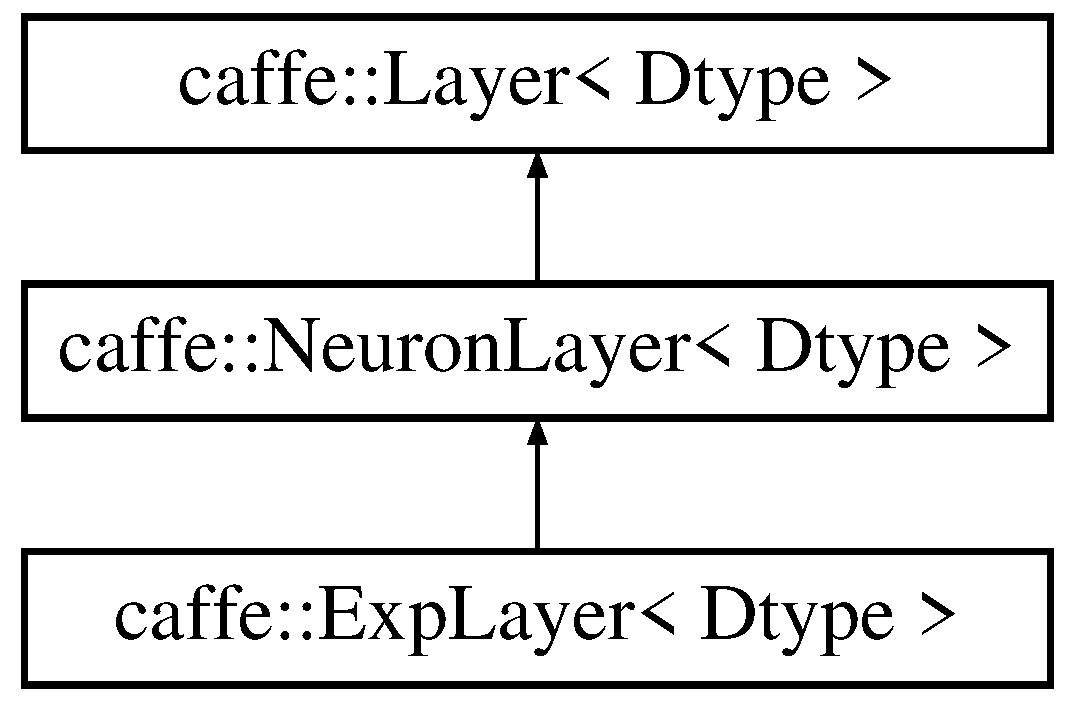
\includegraphics[height=3.000000cm]{classcaffe_1_1ExpLayer}
\end{center}
\end{figure}
\subsection*{Public Member Functions}
\begin{DoxyCompactItemize}
\item 
\hyperlink{classcaffe_1_1ExpLayer_a87a0fae261ad3d2c8947f463686a6de0}{Exp\+Layer} (const Layer\+Parameter \&param)
\item 
virtual void \hyperlink{classcaffe_1_1ExpLayer_a5f88102bf4922032eeab431154a76710}{Layer\+Set\+Up} (const vector$<$ \hyperlink{classcaffe_1_1Blob}{Blob}$<$ Dtype $>$ $\ast$ $>$ \&bottom, const vector$<$ \hyperlink{classcaffe_1_1Blob}{Blob}$<$ Dtype $>$ $\ast$ $>$ \&top)
\begin{DoxyCompactList}\small\item\em Does layer-\/specific setup\+: your layer should implement this function as well as Reshape. \end{DoxyCompactList}\item 
virtual const char $\ast$ \hyperlink{classcaffe_1_1ExpLayer_a9fce31193341c4f70a65a8670121ab51}{type} () const \hypertarget{classcaffe_1_1ExpLayer_a9fce31193341c4f70a65a8670121ab51}{}\label{classcaffe_1_1ExpLayer_a9fce31193341c4f70a65a8670121ab51}

\begin{DoxyCompactList}\small\item\em Returns the layer type. \end{DoxyCompactList}\end{DoxyCompactItemize}
\subsection*{Protected Member Functions}
\begin{DoxyCompactItemize}
\item 
virtual void \hyperlink{classcaffe_1_1ExpLayer_a56e2e4d6b5bc7eb5d7242f216bd70961}{Forward\+\_\+cpu} (const vector$<$ \hyperlink{classcaffe_1_1Blob}{Blob}$<$ Dtype $>$ $\ast$ $>$ \&bottom, const vector$<$ \hyperlink{classcaffe_1_1Blob}{Blob}$<$ Dtype $>$ $\ast$ $>$ \&top)
\item 
virtual void \hyperlink{classcaffe_1_1ExpLayer_a3d6df27bfdb0aac45f5a7682e0ad7e3f}{Forward\+\_\+gpu} (const vector$<$ \hyperlink{classcaffe_1_1Blob}{Blob}$<$ Dtype $>$ $\ast$ $>$ \&bottom, const vector$<$ \hyperlink{classcaffe_1_1Blob}{Blob}$<$ Dtype $>$ $\ast$ $>$ \&top)\hypertarget{classcaffe_1_1ExpLayer_a3d6df27bfdb0aac45f5a7682e0ad7e3f}{}\label{classcaffe_1_1ExpLayer_a3d6df27bfdb0aac45f5a7682e0ad7e3f}

\begin{DoxyCompactList}\small\item\em Using the G\+PU device, compute the layer output. Fall back to \hyperlink{classcaffe_1_1ExpLayer_a56e2e4d6b5bc7eb5d7242f216bd70961}{Forward\+\_\+cpu()} if unavailable. \end{DoxyCompactList}\item 
virtual void \hyperlink{classcaffe_1_1ExpLayer_a691eeee0b9b2cbd1742e1fde7ba4d941}{Backward\+\_\+cpu} (const vector$<$ \hyperlink{classcaffe_1_1Blob}{Blob}$<$ Dtype $>$ $\ast$ $>$ \&top, const vector$<$ bool $>$ \&propagate\+\_\+down, const vector$<$ \hyperlink{classcaffe_1_1Blob}{Blob}$<$ Dtype $>$ $\ast$ $>$ \&bottom)
\begin{DoxyCompactList}\small\item\em Computes the error gradient w.\+r.\+t. the exp inputs. \end{DoxyCompactList}\item 
virtual void \hyperlink{classcaffe_1_1ExpLayer_a2a1b0a09970aa4998f9f409609ed3712}{Backward\+\_\+gpu} (const vector$<$ \hyperlink{classcaffe_1_1Blob}{Blob}$<$ Dtype $>$ $\ast$ $>$ \&top, const vector$<$ bool $>$ \&propagate\+\_\+down, const vector$<$ \hyperlink{classcaffe_1_1Blob}{Blob}$<$ Dtype $>$ $\ast$ $>$ \&bottom)\hypertarget{classcaffe_1_1ExpLayer_a2a1b0a09970aa4998f9f409609ed3712}{}\label{classcaffe_1_1ExpLayer_a2a1b0a09970aa4998f9f409609ed3712}

\begin{DoxyCompactList}\small\item\em Using the G\+PU device, compute the gradients for any parameters and for the bottom blobs if propagate\+\_\+down is true. Fall back to \hyperlink{classcaffe_1_1ExpLayer_a691eeee0b9b2cbd1742e1fde7ba4d941}{Backward\+\_\+cpu()} if unavailable. \end{DoxyCompactList}\end{DoxyCompactItemize}
\subsection*{Protected Attributes}
\begin{DoxyCompactItemize}
\item 
Dtype {\bfseries inner\+\_\+scale\+\_\+}\hypertarget{classcaffe_1_1ExpLayer_a60dd67dcdc7c46fb4514f25a56e43cce}{}\label{classcaffe_1_1ExpLayer_a60dd67dcdc7c46fb4514f25a56e43cce}

\item 
Dtype {\bfseries outer\+\_\+scale\+\_\+}\hypertarget{classcaffe_1_1ExpLayer_aeb8e9967b8c9cb57a4ff2f797dc6a36a}{}\label{classcaffe_1_1ExpLayer_aeb8e9967b8c9cb57a4ff2f797dc6a36a}

\end{DoxyCompactItemize}


\subsection{Detailed Description}
\subsubsection*{template$<$typename Dtype$>$\\*
class caffe\+::\+Exp\+Layer$<$ Dtype $>$}

Computes $ y = \gamma ^ {\alpha x + \beta} $, as specified by the scale $ \alpha $, shift $ \beta $, and base $ \gamma $. 

\subsection{Constructor \& Destructor Documentation}
\index{caffe\+::\+Exp\+Layer@{caffe\+::\+Exp\+Layer}!Exp\+Layer@{Exp\+Layer}}
\index{Exp\+Layer@{Exp\+Layer}!caffe\+::\+Exp\+Layer@{caffe\+::\+Exp\+Layer}}
\subsubsection[{\texorpdfstring{Exp\+Layer(const Layer\+Parameter \&param)}{ExpLayer(const LayerParameter &param)}}]{\setlength{\rightskip}{0pt plus 5cm}template$<$typename Dtype $>$ {\bf caffe\+::\+Exp\+Layer}$<$ Dtype $>$\+::{\bf Exp\+Layer} (
\begin{DoxyParamCaption}
\item[{const Layer\+Parameter \&}]{param}
\end{DoxyParamCaption}
)\hspace{0.3cm}{\ttfamily [inline]}, {\ttfamily [explicit]}}\hypertarget{classcaffe_1_1ExpLayer_a87a0fae261ad3d2c8947f463686a6de0}{}\label{classcaffe_1_1ExpLayer_a87a0fae261ad3d2c8947f463686a6de0}

\begin{DoxyParams}{Parameters}
{\em param} & provides Exp\+Parameter exp\+\_\+param, with \hyperlink{classcaffe_1_1ExpLayer}{Exp\+Layer} options\+:
\begin{DoxyItemize}
\item scale ({\bfseries optional}, default 1) the scale $ \alpha $
\item shift ({\bfseries optional}, default 0) the shift $ \beta $
\item base ({\bfseries optional}, default -\/1 for a value of $ e \approx 2.718 $) the base $ \gamma $ 
\end{DoxyItemize}\\
\hline
\end{DoxyParams}


\subsection{Member Function Documentation}
\index{caffe\+::\+Exp\+Layer@{caffe\+::\+Exp\+Layer}!Backward\+\_\+cpu@{Backward\+\_\+cpu}}
\index{Backward\+\_\+cpu@{Backward\+\_\+cpu}!caffe\+::\+Exp\+Layer@{caffe\+::\+Exp\+Layer}}
\subsubsection[{\texorpdfstring{Backward\+\_\+cpu(const vector$<$ Blob$<$ Dtype $>$ $\ast$ $>$ \&top, const vector$<$ bool $>$ \&propagate\+\_\+down, const vector$<$ Blob$<$ Dtype $>$ $\ast$ $>$ \&bottom)}{Backward_cpu(const vector< Blob< Dtype > * > &top, const vector< bool > &propagate_down, const vector< Blob< Dtype > * > &bottom)}}]{\setlength{\rightskip}{0pt plus 5cm}template$<$typename Dtype $>$ void {\bf caffe\+::\+Exp\+Layer}$<$ Dtype $>$\+::Backward\+\_\+cpu (
\begin{DoxyParamCaption}
\item[{const vector$<$ {\bf Blob}$<$ Dtype $>$ $\ast$ $>$ \&}]{top, }
\item[{const vector$<$ bool $>$ \&}]{propagate\+\_\+down, }
\item[{const vector$<$ {\bf Blob}$<$ Dtype $>$ $\ast$ $>$ \&}]{bottom}
\end{DoxyParamCaption}
)\hspace{0.3cm}{\ttfamily [protected]}, {\ttfamily [virtual]}}\hypertarget{classcaffe_1_1ExpLayer_a691eeee0b9b2cbd1742e1fde7ba4d941}{}\label{classcaffe_1_1ExpLayer_a691eeee0b9b2cbd1742e1fde7ba4d941}


Computes the error gradient w.\+r.\+t. the exp inputs. 


\begin{DoxyParams}{Parameters}
{\em top} & output \hyperlink{classcaffe_1_1Blob}{Blob} vector (length 1), providing the error gradient with respect to the outputs
\begin{DoxyEnumerate}
\item $ (N \times C \times H \times W) $ containing error gradients $ \frac{\partial E}{\partial y} $ with respect to computed outputs $ y $ 
\end{DoxyEnumerate}\\
\hline
{\em propagate\+\_\+down} & see \hyperlink{classcaffe_1_1Layer_a53df1e081767e07bfb4c81657f4acd0a}{Layer\+::\+Backward}. \\
\hline
{\em bottom} & input \hyperlink{classcaffe_1_1Blob}{Blob} vector (length 1)
\begin{DoxyEnumerate}
\item $ (N \times C \times H \times W) $ the inputs $ x $; Backward fills their diff with gradients $ \frac{\partial E}{\partial x} = \frac{\partial E}{\partial y} y \alpha \log_e(gamma) $ if propagate\+\_\+down\mbox{[}0\mbox{]} 
\end{DoxyEnumerate}\\
\hline
\end{DoxyParams}


Implements \hyperlink{classcaffe_1_1Layer_a64d15855f882af4b82e83fa993c4e7c6}{caffe\+::\+Layer$<$ Dtype $>$}.

\index{caffe\+::\+Exp\+Layer@{caffe\+::\+Exp\+Layer}!Forward\+\_\+cpu@{Forward\+\_\+cpu}}
\index{Forward\+\_\+cpu@{Forward\+\_\+cpu}!caffe\+::\+Exp\+Layer@{caffe\+::\+Exp\+Layer}}
\subsubsection[{\texorpdfstring{Forward\+\_\+cpu(const vector$<$ Blob$<$ Dtype $>$ $\ast$ $>$ \&bottom, const vector$<$ Blob$<$ Dtype $>$ $\ast$ $>$ \&top)}{Forward_cpu(const vector< Blob< Dtype > * > &bottom, const vector< Blob< Dtype > * > &top)}}]{\setlength{\rightskip}{0pt plus 5cm}template$<$typename Dtype $>$ void {\bf caffe\+::\+Exp\+Layer}$<$ Dtype $>$\+::Forward\+\_\+cpu (
\begin{DoxyParamCaption}
\item[{const vector$<$ {\bf Blob}$<$ Dtype $>$ $\ast$ $>$ \&}]{bottom, }
\item[{const vector$<$ {\bf Blob}$<$ Dtype $>$ $\ast$ $>$ \&}]{top}
\end{DoxyParamCaption}
)\hspace{0.3cm}{\ttfamily [protected]}, {\ttfamily [virtual]}}\hypertarget{classcaffe_1_1ExpLayer_a56e2e4d6b5bc7eb5d7242f216bd70961}{}\label{classcaffe_1_1ExpLayer_a56e2e4d6b5bc7eb5d7242f216bd70961}

\begin{DoxyParams}{Parameters}
{\em bottom} & input \hyperlink{classcaffe_1_1Blob}{Blob} vector (length 1)
\begin{DoxyEnumerate}
\item $ (N \times C \times H \times W) $ the inputs $ x $ 
\end{DoxyEnumerate}\\
\hline
{\em top} & output \hyperlink{classcaffe_1_1Blob}{Blob} vector (length 1)
\begin{DoxyEnumerate}
\item $ (N \times C \times H \times W) $ the computed outputs $ y = \gamma ^ {\alpha x + \beta} $ 
\end{DoxyEnumerate}\\
\hline
\end{DoxyParams}


Implements \hyperlink{classcaffe_1_1Layer_add965883f75bbf90c7a06f960cda7a1a}{caffe\+::\+Layer$<$ Dtype $>$}.

\index{caffe\+::\+Exp\+Layer@{caffe\+::\+Exp\+Layer}!Layer\+Set\+Up@{Layer\+Set\+Up}}
\index{Layer\+Set\+Up@{Layer\+Set\+Up}!caffe\+::\+Exp\+Layer@{caffe\+::\+Exp\+Layer}}
\subsubsection[{\texorpdfstring{Layer\+Set\+Up(const vector$<$ Blob$<$ Dtype $>$ $\ast$ $>$ \&bottom, const vector$<$ Blob$<$ Dtype $>$ $\ast$ $>$ \&top)}{LayerSetUp(const vector< Blob< Dtype > * > &bottom, const vector< Blob< Dtype > * > &top)}}]{\setlength{\rightskip}{0pt plus 5cm}template$<$typename Dtype $>$ void {\bf caffe\+::\+Exp\+Layer}$<$ Dtype $>$\+::Layer\+Set\+Up (
\begin{DoxyParamCaption}
\item[{const vector$<$ {\bf Blob}$<$ Dtype $>$ $\ast$ $>$ \&}]{bottom, }
\item[{const vector$<$ {\bf Blob}$<$ Dtype $>$ $\ast$ $>$ \&}]{top}
\end{DoxyParamCaption}
)\hspace{0.3cm}{\ttfamily [virtual]}}\hypertarget{classcaffe_1_1ExpLayer_a5f88102bf4922032eeab431154a76710}{}\label{classcaffe_1_1ExpLayer_a5f88102bf4922032eeab431154a76710}


Does layer-\/specific setup\+: your layer should implement this function as well as Reshape. 


\begin{DoxyParams}{Parameters}
{\em bottom} & the preshaped input blobs, whose data fields store the input data for this layer \\
\hline
{\em top} & the allocated but unshaped output blobs\\
\hline
\end{DoxyParams}
This method should do one-\/time layer specific setup. This includes reading and processing relevent parameters from the {\ttfamily layer\+\_\+param\+\_\+}. Setting up the shapes of top blobs and internal buffers should be done in {\ttfamily Reshape}, which will be called before the forward pass to adjust the top blob sizes. 

Reimplemented from \hyperlink{classcaffe_1_1Layer_a38dc2488bf319b8de5a7ac84e0045393}{caffe\+::\+Layer$<$ Dtype $>$}.



The documentation for this class was generated from the following files\+:\begin{DoxyCompactItemize}
\item 
include/caffe/layers/exp\+\_\+layer.\+hpp\item 
src/caffe/layers/exp\+\_\+layer.\+cpp\end{DoxyCompactItemize}

\hypertarget{classcaffe_1_1Filler}{}\section{caffe\+:\+:Filler$<$ Dtype $>$ Class Template Reference}
\label{classcaffe_1_1Filler}\index{caffe\+::\+Filler$<$ Dtype $>$@{caffe\+::\+Filler$<$ Dtype $>$}}


Fills a \hyperlink{classcaffe_1_1Blob}{Blob} with constant or randomly-\/generated data.  




{\ttfamily \#include $<$filler.\+hpp$>$}

Inheritance diagram for caffe\+:\+:Filler$<$ Dtype $>$\+:\begin{figure}[H]
\begin{center}
\leavevmode
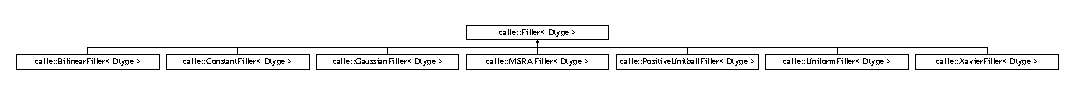
\includegraphics[height=0.707965cm]{classcaffe_1_1Filler}
\end{center}
\end{figure}
\subsection*{Public Member Functions}
\begin{DoxyCompactItemize}
\item 
{\bfseries Filler} (const Filler\+Parameter \&param)\hypertarget{classcaffe_1_1Filler_aff156b1d4e5dbbbad720aa776df44512}{}\label{classcaffe_1_1Filler_aff156b1d4e5dbbbad720aa776df44512}

\item 
virtual void {\bfseries Fill} (\hyperlink{classcaffe_1_1Blob}{Blob}$<$ Dtype $>$ $\ast$blob)=0\hypertarget{classcaffe_1_1Filler_acd02177b669381252a7c484f51432d30}{}\label{classcaffe_1_1Filler_acd02177b669381252a7c484f51432d30}

\end{DoxyCompactItemize}
\subsection*{Protected Attributes}
\begin{DoxyCompactItemize}
\item 
Filler\+Parameter {\bfseries filler\+\_\+param\+\_\+}\hypertarget{classcaffe_1_1Filler_a1ded14cf43eeb7b45628770842c4348c}{}\label{classcaffe_1_1Filler_a1ded14cf43eeb7b45628770842c4348c}

\end{DoxyCompactItemize}


\subsection{Detailed Description}
\subsubsection*{template$<$typename Dtype$>$\\*
class caffe\+::\+Filler$<$ Dtype $>$}

Fills a \hyperlink{classcaffe_1_1Blob}{Blob} with constant or randomly-\/generated data. 

The documentation for this class was generated from the following file\+:\begin{DoxyCompactItemize}
\item 
include/caffe/filler.\+hpp\end{DoxyCompactItemize}

\hypertarget{classcaffe_1_1FilterLayer}{}\section{caffe\+:\+:Filter\+Layer$<$ Dtype $>$ Class Template Reference}
\label{classcaffe_1_1FilterLayer}\index{caffe\+::\+Filter\+Layer$<$ Dtype $>$@{caffe\+::\+Filter\+Layer$<$ Dtype $>$}}


Takes two+ Blobs, interprets last \hyperlink{classcaffe_1_1Blob}{Blob} as a selector and filter remaining Blobs accordingly with selector data (0 means that the corresponding item has to be filtered, non-\/zero means that corresponding item needs to stay).  




{\ttfamily \#include $<$filter\+\_\+layer.\+hpp$>$}

Inheritance diagram for caffe\+:\+:Filter\+Layer$<$ Dtype $>$\+:\begin{figure}[H]
\begin{center}
\leavevmode
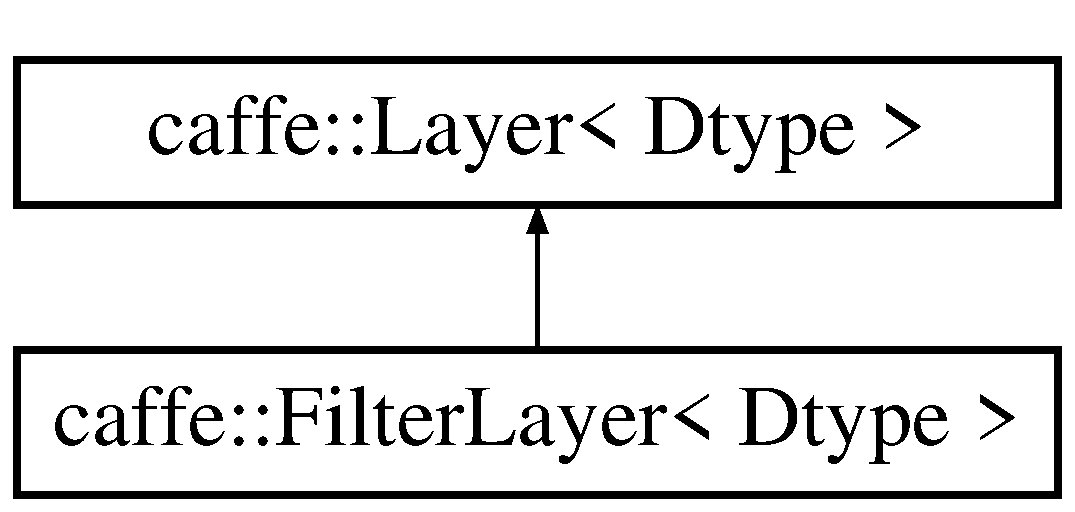
\includegraphics[height=2.000000cm]{classcaffe_1_1FilterLayer}
\end{center}
\end{figure}
\subsection*{Public Member Functions}
\begin{DoxyCompactItemize}
\item 
{\bfseries Filter\+Layer} (const Layer\+Parameter \&param)\hypertarget{classcaffe_1_1FilterLayer_a7384a8e15c84b16b46b775a11b95cc4f}{}\label{classcaffe_1_1FilterLayer_a7384a8e15c84b16b46b775a11b95cc4f}

\item 
virtual void \hyperlink{classcaffe_1_1FilterLayer_acbbb4dd26fd8a5ab01bce9aa34ad12ae}{Layer\+Set\+Up} (const vector$<$ \hyperlink{classcaffe_1_1Blob}{Blob}$<$ Dtype $>$ $\ast$ $>$ \&bottom, const vector$<$ \hyperlink{classcaffe_1_1Blob}{Blob}$<$ Dtype $>$ $\ast$ $>$ \&top)
\begin{DoxyCompactList}\small\item\em Does layer-\/specific setup\+: your layer should implement this function as well as Reshape. \end{DoxyCompactList}\item 
virtual void \hyperlink{classcaffe_1_1FilterLayer_a38ca56415d59b1d89c8fd4b4b25da2de}{Reshape} (const vector$<$ \hyperlink{classcaffe_1_1Blob}{Blob}$<$ Dtype $>$ $\ast$ $>$ \&bottom, const vector$<$ \hyperlink{classcaffe_1_1Blob}{Blob}$<$ Dtype $>$ $\ast$ $>$ \&top)
\begin{DoxyCompactList}\small\item\em Adjust the shapes of top blobs and internal buffers to accommodate the shapes of the bottom blobs. \end{DoxyCompactList}\item 
virtual const char $\ast$ \hyperlink{classcaffe_1_1FilterLayer_aaca9f27ee4bc34889817256ed643d433}{type} () const \hypertarget{classcaffe_1_1FilterLayer_aaca9f27ee4bc34889817256ed643d433}{}\label{classcaffe_1_1FilterLayer_aaca9f27ee4bc34889817256ed643d433}

\begin{DoxyCompactList}\small\item\em Returns the layer type. \end{DoxyCompactList}\item 
virtual int \hyperlink{classcaffe_1_1FilterLayer_a13119969cca3f6d1b4b3fea77619d595}{Min\+Bottom\+Blobs} () const 
\begin{DoxyCompactList}\small\item\em Returns the minimum number of bottom blobs required by the layer, or -\/1 if no minimum number is required. \end{DoxyCompactList}\item 
virtual int \hyperlink{classcaffe_1_1FilterLayer_abae0953d9773e25b7cfc5bdea4f6230a}{Min\+Top\+Blobs} () const 
\begin{DoxyCompactList}\small\item\em Returns the minimum number of top blobs required by the layer, or -\/1 if no minimum number is required. \end{DoxyCompactList}\end{DoxyCompactItemize}
\subsection*{Protected Member Functions}
\begin{DoxyCompactItemize}
\item 
virtual void \hyperlink{classcaffe_1_1FilterLayer_a57b597be559867696898b34ff5fe6338}{Forward\+\_\+cpu} (const vector$<$ \hyperlink{classcaffe_1_1Blob}{Blob}$<$ Dtype $>$ $\ast$ $>$ \&bottom, const vector$<$ \hyperlink{classcaffe_1_1Blob}{Blob}$<$ Dtype $>$ $\ast$ $>$ \&top)
\item 
virtual void \hyperlink{classcaffe_1_1FilterLayer_ae9037245327193ba8d42f274b9fcfda8}{Forward\+\_\+gpu} (const vector$<$ \hyperlink{classcaffe_1_1Blob}{Blob}$<$ Dtype $>$ $\ast$ $>$ \&bottom, const vector$<$ \hyperlink{classcaffe_1_1Blob}{Blob}$<$ Dtype $>$ $\ast$ $>$ \&top)\hypertarget{classcaffe_1_1FilterLayer_ae9037245327193ba8d42f274b9fcfda8}{}\label{classcaffe_1_1FilterLayer_ae9037245327193ba8d42f274b9fcfda8}

\begin{DoxyCompactList}\small\item\em Using the G\+PU device, compute the layer output. Fall back to \hyperlink{classcaffe_1_1FilterLayer_a57b597be559867696898b34ff5fe6338}{Forward\+\_\+cpu()} if unavailable. \end{DoxyCompactList}\item 
virtual void \hyperlink{classcaffe_1_1FilterLayer_abaf7065db8ab50d5ef6a4acff85a0aeb}{Backward\+\_\+cpu} (const vector$<$ \hyperlink{classcaffe_1_1Blob}{Blob}$<$ Dtype $>$ $\ast$ $>$ \&top, const vector$<$ bool $>$ \&propagate\+\_\+down, const vector$<$ \hyperlink{classcaffe_1_1Blob}{Blob}$<$ Dtype $>$ $\ast$ $>$ \&bottom)
\begin{DoxyCompactList}\small\item\em Computes the error gradient w.\+r.\+t. the forwarded inputs. \end{DoxyCompactList}\item 
virtual void \hyperlink{classcaffe_1_1FilterLayer_a00f33332f047badddb94f04b7d892def}{Backward\+\_\+gpu} (const vector$<$ \hyperlink{classcaffe_1_1Blob}{Blob}$<$ Dtype $>$ $\ast$ $>$ \&top, const vector$<$ bool $>$ \&propagate\+\_\+down, const vector$<$ \hyperlink{classcaffe_1_1Blob}{Blob}$<$ Dtype $>$ $\ast$ $>$ \&bottom)\hypertarget{classcaffe_1_1FilterLayer_a00f33332f047badddb94f04b7d892def}{}\label{classcaffe_1_1FilterLayer_a00f33332f047badddb94f04b7d892def}

\begin{DoxyCompactList}\small\item\em Using the G\+PU device, compute the gradients for any parameters and for the bottom blobs if propagate\+\_\+down is true. Fall back to \hyperlink{classcaffe_1_1FilterLayer_abaf7065db8ab50d5ef6a4acff85a0aeb}{Backward\+\_\+cpu()} if unavailable. \end{DoxyCompactList}\end{DoxyCompactItemize}
\subsection*{Protected Attributes}
\begin{DoxyCompactItemize}
\item 
bool {\bfseries first\+\_\+reshape\+\_\+}\hypertarget{classcaffe_1_1FilterLayer_a0bfd8003e455c2f3a67172247058604b}{}\label{classcaffe_1_1FilterLayer_a0bfd8003e455c2f3a67172247058604b}

\item 
vector$<$ int $>$ {\bfseries indices\+\_\+to\+\_\+forward\+\_\+}\hypertarget{classcaffe_1_1FilterLayer_a3a53a99be807ac5e50de8fe7e6825c59}{}\label{classcaffe_1_1FilterLayer_a3a53a99be807ac5e50de8fe7e6825c59}

\end{DoxyCompactItemize}


\subsection{Detailed Description}
\subsubsection*{template$<$typename Dtype$>$\\*
class caffe\+::\+Filter\+Layer$<$ Dtype $>$}

Takes two+ Blobs, interprets last \hyperlink{classcaffe_1_1Blob}{Blob} as a selector and filter remaining Blobs accordingly with selector data (0 means that the corresponding item has to be filtered, non-\/zero means that corresponding item needs to stay). 

\subsection{Member Function Documentation}
\index{caffe\+::\+Filter\+Layer@{caffe\+::\+Filter\+Layer}!Backward\+\_\+cpu@{Backward\+\_\+cpu}}
\index{Backward\+\_\+cpu@{Backward\+\_\+cpu}!caffe\+::\+Filter\+Layer@{caffe\+::\+Filter\+Layer}}
\subsubsection[{\texorpdfstring{Backward\+\_\+cpu(const vector$<$ Blob$<$ Dtype $>$ $\ast$ $>$ \&top, const vector$<$ bool $>$ \&propagate\+\_\+down, const vector$<$ Blob$<$ Dtype $>$ $\ast$ $>$ \&bottom)}{Backward_cpu(const vector< Blob< Dtype > * > &top, const vector< bool > &propagate_down, const vector< Blob< Dtype > * > &bottom)}}]{\setlength{\rightskip}{0pt plus 5cm}template$<$typename Dtype $>$ void {\bf caffe\+::\+Filter\+Layer}$<$ Dtype $>$\+::Backward\+\_\+cpu (
\begin{DoxyParamCaption}
\item[{const vector$<$ {\bf Blob}$<$ Dtype $>$ $\ast$ $>$ \&}]{top, }
\item[{const vector$<$ bool $>$ \&}]{propagate\+\_\+down, }
\item[{const vector$<$ {\bf Blob}$<$ Dtype $>$ $\ast$ $>$ \&}]{bottom}
\end{DoxyParamCaption}
)\hspace{0.3cm}{\ttfamily [protected]}, {\ttfamily [virtual]}}\hypertarget{classcaffe_1_1FilterLayer_abaf7065db8ab50d5ef6a4acff85a0aeb}{}\label{classcaffe_1_1FilterLayer_abaf7065db8ab50d5ef6a4acff85a0aeb}


Computes the error gradient w.\+r.\+t. the forwarded inputs. 


\begin{DoxyParams}{Parameters}
{\em top} & output \hyperlink{classcaffe_1_1Blob}{Blob} vector (length 1+), providing the error gradient with respect to the outputs \\
\hline
{\em propagate\+\_\+down} & see \hyperlink{classcaffe_1_1Layer_a53df1e081767e07bfb4c81657f4acd0a}{Layer\+::\+Backward}. \\
\hline
{\em bottom} & input \hyperlink{classcaffe_1_1Blob}{Blob} vector (length 2+), into which the top error gradient is copied \\
\hline
\end{DoxyParams}


Implements \hyperlink{classcaffe_1_1Layer_a64d15855f882af4b82e83fa993c4e7c6}{caffe\+::\+Layer$<$ Dtype $>$}.

\index{caffe\+::\+Filter\+Layer@{caffe\+::\+Filter\+Layer}!Forward\+\_\+cpu@{Forward\+\_\+cpu}}
\index{Forward\+\_\+cpu@{Forward\+\_\+cpu}!caffe\+::\+Filter\+Layer@{caffe\+::\+Filter\+Layer}}
\subsubsection[{\texorpdfstring{Forward\+\_\+cpu(const vector$<$ Blob$<$ Dtype $>$ $\ast$ $>$ \&bottom, const vector$<$ Blob$<$ Dtype $>$ $\ast$ $>$ \&top)}{Forward_cpu(const vector< Blob< Dtype > * > &bottom, const vector< Blob< Dtype > * > &top)}}]{\setlength{\rightskip}{0pt plus 5cm}template$<$typename Dtype $>$ void {\bf caffe\+::\+Filter\+Layer}$<$ Dtype $>$\+::Forward\+\_\+cpu (
\begin{DoxyParamCaption}
\item[{const vector$<$ {\bf Blob}$<$ Dtype $>$ $\ast$ $>$ \&}]{bottom, }
\item[{const vector$<$ {\bf Blob}$<$ Dtype $>$ $\ast$ $>$ \&}]{top}
\end{DoxyParamCaption}
)\hspace{0.3cm}{\ttfamily [protected]}, {\ttfamily [virtual]}}\hypertarget{classcaffe_1_1FilterLayer_a57b597be559867696898b34ff5fe6338}{}\label{classcaffe_1_1FilterLayer_a57b597be559867696898b34ff5fe6338}

\begin{DoxyParams}{Parameters}
{\em bottom} & input \hyperlink{classcaffe_1_1Blob}{Blob} vector (length 2+)
\begin{DoxyEnumerate}
\item $ (N \times C \times H \times W) $ the inputs to be filtered $ x_1 $
\item ...
\item $ (N \times C \times H \times W) $ the inputs to be filtered $ x_K $
\item $ (N \times 1 \times 1 \times 1) $ the selector blob 
\end{DoxyEnumerate}\\
\hline
{\em top} & output \hyperlink{classcaffe_1_1Blob}{Blob} vector (length 1+)
\begin{DoxyEnumerate}
\item $ (S \times C \times H \times W) $ () the filtered output $ x_1 $ where S is the number of items that haven\textquotesingle{}t been filtered $ (S \times C \times H \times W) $ the filtered output $ x_K $ where S is the number of items that haven\textquotesingle{}t been filtered 
\end{DoxyEnumerate}\\
\hline
\end{DoxyParams}


Implements \hyperlink{classcaffe_1_1Layer_add965883f75bbf90c7a06f960cda7a1a}{caffe\+::\+Layer$<$ Dtype $>$}.

\index{caffe\+::\+Filter\+Layer@{caffe\+::\+Filter\+Layer}!Layer\+Set\+Up@{Layer\+Set\+Up}}
\index{Layer\+Set\+Up@{Layer\+Set\+Up}!caffe\+::\+Filter\+Layer@{caffe\+::\+Filter\+Layer}}
\subsubsection[{\texorpdfstring{Layer\+Set\+Up(const vector$<$ Blob$<$ Dtype $>$ $\ast$ $>$ \&bottom, const vector$<$ Blob$<$ Dtype $>$ $\ast$ $>$ \&top)}{LayerSetUp(const vector< Blob< Dtype > * > &bottom, const vector< Blob< Dtype > * > &top)}}]{\setlength{\rightskip}{0pt plus 5cm}template$<$typename Dtype $>$ void {\bf caffe\+::\+Filter\+Layer}$<$ Dtype $>$\+::Layer\+Set\+Up (
\begin{DoxyParamCaption}
\item[{const vector$<$ {\bf Blob}$<$ Dtype $>$ $\ast$ $>$ \&}]{bottom, }
\item[{const vector$<$ {\bf Blob}$<$ Dtype $>$ $\ast$ $>$ \&}]{top}
\end{DoxyParamCaption}
)\hspace{0.3cm}{\ttfamily [virtual]}}\hypertarget{classcaffe_1_1FilterLayer_acbbb4dd26fd8a5ab01bce9aa34ad12ae}{}\label{classcaffe_1_1FilterLayer_acbbb4dd26fd8a5ab01bce9aa34ad12ae}


Does layer-\/specific setup\+: your layer should implement this function as well as Reshape. 


\begin{DoxyParams}{Parameters}
{\em bottom} & the preshaped input blobs, whose data fields store the input data for this layer \\
\hline
{\em top} & the allocated but unshaped output blobs\\
\hline
\end{DoxyParams}
This method should do one-\/time layer specific setup. This includes reading and processing relevent parameters from the {\ttfamily layer\+\_\+param\+\_\+}. Setting up the shapes of top blobs and internal buffers should be done in {\ttfamily Reshape}, which will be called before the forward pass to adjust the top blob sizes. 

Reimplemented from \hyperlink{classcaffe_1_1Layer_a38dc2488bf319b8de5a7ac84e0045393}{caffe\+::\+Layer$<$ Dtype $>$}.

\index{caffe\+::\+Filter\+Layer@{caffe\+::\+Filter\+Layer}!Min\+Bottom\+Blobs@{Min\+Bottom\+Blobs}}
\index{Min\+Bottom\+Blobs@{Min\+Bottom\+Blobs}!caffe\+::\+Filter\+Layer@{caffe\+::\+Filter\+Layer}}
\subsubsection[{\texorpdfstring{Min\+Bottom\+Blobs() const }{MinBottomBlobs() const }}]{\setlength{\rightskip}{0pt plus 5cm}template$<$typename Dtype $>$ virtual int {\bf caffe\+::\+Filter\+Layer}$<$ Dtype $>$\+::Min\+Bottom\+Blobs (
\begin{DoxyParamCaption}
{}
\end{DoxyParamCaption}
) const\hspace{0.3cm}{\ttfamily [inline]}, {\ttfamily [virtual]}}\hypertarget{classcaffe_1_1FilterLayer_a13119969cca3f6d1b4b3fea77619d595}{}\label{classcaffe_1_1FilterLayer_a13119969cca3f6d1b4b3fea77619d595}


Returns the minimum number of bottom blobs required by the layer, or -\/1 if no minimum number is required. 

This method should be overridden to return a non-\/negative value if your layer expects some minimum number of bottom blobs. 

Reimplemented from \hyperlink{classcaffe_1_1Layer_ade3eee97cc743c4e68fff7eba6484916}{caffe\+::\+Layer$<$ Dtype $>$}.

\index{caffe\+::\+Filter\+Layer@{caffe\+::\+Filter\+Layer}!Min\+Top\+Blobs@{Min\+Top\+Blobs}}
\index{Min\+Top\+Blobs@{Min\+Top\+Blobs}!caffe\+::\+Filter\+Layer@{caffe\+::\+Filter\+Layer}}
\subsubsection[{\texorpdfstring{Min\+Top\+Blobs() const }{MinTopBlobs() const }}]{\setlength{\rightskip}{0pt plus 5cm}template$<$typename Dtype $>$ virtual int {\bf caffe\+::\+Filter\+Layer}$<$ Dtype $>$\+::Min\+Top\+Blobs (
\begin{DoxyParamCaption}
{}
\end{DoxyParamCaption}
) const\hspace{0.3cm}{\ttfamily [inline]}, {\ttfamily [virtual]}}\hypertarget{classcaffe_1_1FilterLayer_abae0953d9773e25b7cfc5bdea4f6230a}{}\label{classcaffe_1_1FilterLayer_abae0953d9773e25b7cfc5bdea4f6230a}


Returns the minimum number of top blobs required by the layer, or -\/1 if no minimum number is required. 

This method should be overridden to return a non-\/negative value if your layer expects some minimum number of top blobs. 

Reimplemented from \hyperlink{classcaffe_1_1Layer_a8bb143d58a740345fa2dc3d4204d553b}{caffe\+::\+Layer$<$ Dtype $>$}.

\index{caffe\+::\+Filter\+Layer@{caffe\+::\+Filter\+Layer}!Reshape@{Reshape}}
\index{Reshape@{Reshape}!caffe\+::\+Filter\+Layer@{caffe\+::\+Filter\+Layer}}
\subsubsection[{\texorpdfstring{Reshape(const vector$<$ Blob$<$ Dtype $>$ $\ast$ $>$ \&bottom, const vector$<$ Blob$<$ Dtype $>$ $\ast$ $>$ \&top)}{Reshape(const vector< Blob< Dtype > * > &bottom, const vector< Blob< Dtype > * > &top)}}]{\setlength{\rightskip}{0pt plus 5cm}template$<$typename Dtype $>$ void {\bf caffe\+::\+Filter\+Layer}$<$ Dtype $>$\+::Reshape (
\begin{DoxyParamCaption}
\item[{const vector$<$ {\bf Blob}$<$ Dtype $>$ $\ast$ $>$ \&}]{bottom, }
\item[{const vector$<$ {\bf Blob}$<$ Dtype $>$ $\ast$ $>$ \&}]{top}
\end{DoxyParamCaption}
)\hspace{0.3cm}{\ttfamily [virtual]}}\hypertarget{classcaffe_1_1FilterLayer_a38ca56415d59b1d89c8fd4b4b25da2de}{}\label{classcaffe_1_1FilterLayer_a38ca56415d59b1d89c8fd4b4b25da2de}


Adjust the shapes of top blobs and internal buffers to accommodate the shapes of the bottom blobs. 


\begin{DoxyParams}{Parameters}
{\em bottom} & the input blobs, with the requested input shapes \\
\hline
{\em top} & the top blobs, which should be reshaped as needed\\
\hline
\end{DoxyParams}
This method should reshape top blobs as needed according to the shapes of the bottom (input) blobs, as well as reshaping any internal buffers and making any other necessary adjustments so that the layer can accommodate the bottom blobs. 

Implements \hyperlink{classcaffe_1_1Layer_ad9d391b972c769c0ebee34ca6d1c973e}{caffe\+::\+Layer$<$ Dtype $>$}.



The documentation for this class was generated from the following files\+:\begin{DoxyCompactItemize}
\item 
include/caffe/layers/filter\+\_\+layer.\+hpp\item 
src/caffe/layers/filter\+\_\+layer.\+cpp\end{DoxyCompactItemize}

\hypertarget{classcaffe_1_1FlattenLayer}{}\section{caffe\+:\+:Flatten\+Layer$<$ Dtype $>$ Class Template Reference}
\label{classcaffe_1_1FlattenLayer}\index{caffe\+::\+Flatten\+Layer$<$ Dtype $>$@{caffe\+::\+Flatten\+Layer$<$ Dtype $>$}}


Reshapes the input \hyperlink{classcaffe_1_1Blob}{Blob} into flat vectors.  




{\ttfamily \#include $<$flatten\+\_\+layer.\+hpp$>$}

Inheritance diagram for caffe\+:\+:Flatten\+Layer$<$ Dtype $>$\+:\begin{figure}[H]
\begin{center}
\leavevmode
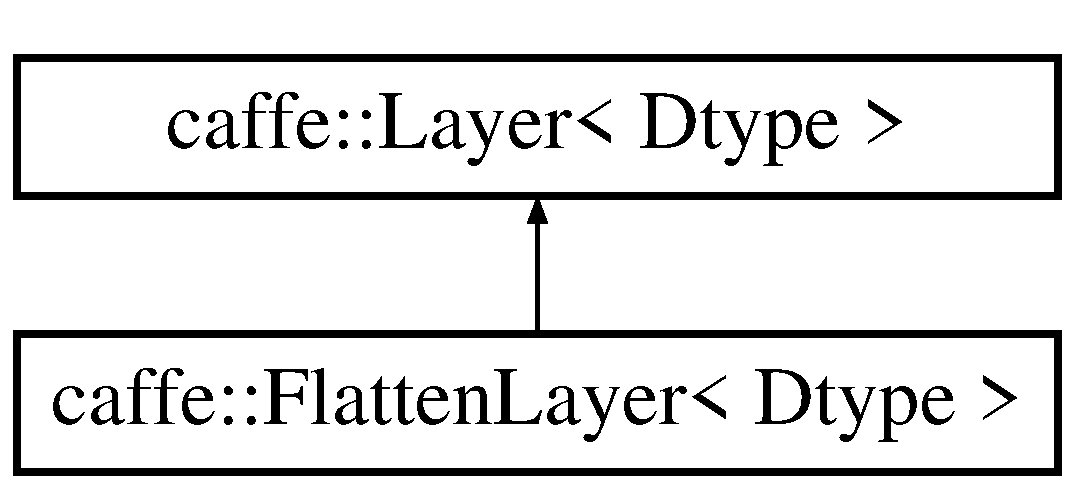
\includegraphics[height=2.000000cm]{classcaffe_1_1FlattenLayer}
\end{center}
\end{figure}
\subsection*{Public Member Functions}
\begin{DoxyCompactItemize}
\item 
{\bfseries Flatten\+Layer} (const Layer\+Parameter \&param)\hypertarget{classcaffe_1_1FlattenLayer_a7ab62567c2fb5424979dc16af273b688}{}\label{classcaffe_1_1FlattenLayer_a7ab62567c2fb5424979dc16af273b688}

\item 
virtual void \hyperlink{classcaffe_1_1FlattenLayer_a1320de156fb152009c13892e30cc87ef}{Reshape} (const vector$<$ \hyperlink{classcaffe_1_1Blob}{Blob}$<$ Dtype $>$ $\ast$ $>$ \&bottom, const vector$<$ \hyperlink{classcaffe_1_1Blob}{Blob}$<$ Dtype $>$ $\ast$ $>$ \&top)
\begin{DoxyCompactList}\small\item\em Adjust the shapes of top blobs and internal buffers to accommodate the shapes of the bottom blobs. \end{DoxyCompactList}\item 
virtual const char $\ast$ \hyperlink{classcaffe_1_1FlattenLayer_a64027633603db57635c844e2c2421d95}{type} () const \hypertarget{classcaffe_1_1FlattenLayer_a64027633603db57635c844e2c2421d95}{}\label{classcaffe_1_1FlattenLayer_a64027633603db57635c844e2c2421d95}

\begin{DoxyCompactList}\small\item\em Returns the layer type. \end{DoxyCompactList}\item 
virtual int \hyperlink{classcaffe_1_1FlattenLayer_ad7abb8ccc06c7943e79d77bf5a7e2521}{Exact\+Num\+Bottom\+Blobs} () const 
\begin{DoxyCompactList}\small\item\em Returns the exact number of bottom blobs required by the layer, or -\/1 if no exact number is required. \end{DoxyCompactList}\item 
virtual int \hyperlink{classcaffe_1_1FlattenLayer_ab54601497218724036abfcec46a718de}{Exact\+Num\+Top\+Blobs} () const 
\begin{DoxyCompactList}\small\item\em Returns the exact number of top blobs required by the layer, or -\/1 if no exact number is required. \end{DoxyCompactList}\end{DoxyCompactItemize}
\subsection*{Protected Member Functions}
\begin{DoxyCompactItemize}
\item 
virtual void \hyperlink{classcaffe_1_1FlattenLayer_a0ecfcc1e1d32ea5ed57ea32f6985d902}{Forward\+\_\+cpu} (const vector$<$ \hyperlink{classcaffe_1_1Blob}{Blob}$<$ Dtype $>$ $\ast$ $>$ \&bottom, const vector$<$ \hyperlink{classcaffe_1_1Blob}{Blob}$<$ Dtype $>$ $\ast$ $>$ \&top)
\item 
virtual void \hyperlink{classcaffe_1_1FlattenLayer_ad207771acf8b2ab912f6daf0c4a6dfe8}{Backward\+\_\+cpu} (const vector$<$ \hyperlink{classcaffe_1_1Blob}{Blob}$<$ Dtype $>$ $\ast$ $>$ \&top, const vector$<$ bool $>$ \&propagate\+\_\+down, const vector$<$ \hyperlink{classcaffe_1_1Blob}{Blob}$<$ Dtype $>$ $\ast$ $>$ \&bottom)
\begin{DoxyCompactList}\small\item\em Computes the error gradient w.\+r.\+t. the concatenate inputs. \end{DoxyCompactList}\end{DoxyCompactItemize}
\subsection*{Additional Inherited Members}


\subsection{Detailed Description}
\subsubsection*{template$<$typename Dtype$>$\\*
class caffe\+::\+Flatten\+Layer$<$ Dtype $>$}

Reshapes the input \hyperlink{classcaffe_1_1Blob}{Blob} into flat vectors. 

Note\+: because this layer does not change the input values -- merely the dimensions -- it can simply copy the input. The copy happens \char`\"{}virtually\char`\"{} (thus taking effectively 0 real time) by setting, in Forward, the data pointer of the top \hyperlink{classcaffe_1_1Blob}{Blob} to that of the bottom \hyperlink{classcaffe_1_1Blob}{Blob} (see \hyperlink{classcaffe_1_1Blob_a8fce5a816a2b9629686db69108610d93}{Blob\+::\+Share\+Data}), and in Backward, the diff pointer of the bottom \hyperlink{classcaffe_1_1Blob}{Blob} to that of the top \hyperlink{classcaffe_1_1Blob}{Blob} (see \hyperlink{classcaffe_1_1Blob_a004781965b09f94c409cec9a6fc7c35c}{Blob\+::\+Share\+Diff}). 

\subsection{Member Function Documentation}
\index{caffe\+::\+Flatten\+Layer@{caffe\+::\+Flatten\+Layer}!Backward\+\_\+cpu@{Backward\+\_\+cpu}}
\index{Backward\+\_\+cpu@{Backward\+\_\+cpu}!caffe\+::\+Flatten\+Layer@{caffe\+::\+Flatten\+Layer}}
\subsubsection[{\texorpdfstring{Backward\+\_\+cpu(const vector$<$ Blob$<$ Dtype $>$ $\ast$ $>$ \&top, const vector$<$ bool $>$ \&propagate\+\_\+down, const vector$<$ Blob$<$ Dtype $>$ $\ast$ $>$ \&bottom)}{Backward_cpu(const vector< Blob< Dtype > * > &top, const vector< bool > &propagate_down, const vector< Blob< Dtype > * > &bottom)}}]{\setlength{\rightskip}{0pt plus 5cm}template$<$typename Dtype $>$ void {\bf caffe\+::\+Flatten\+Layer}$<$ Dtype $>$\+::Backward\+\_\+cpu (
\begin{DoxyParamCaption}
\item[{const vector$<$ {\bf Blob}$<$ Dtype $>$ $\ast$ $>$ \&}]{top, }
\item[{const vector$<$ bool $>$ \&}]{propagate\+\_\+down, }
\item[{const vector$<$ {\bf Blob}$<$ Dtype $>$ $\ast$ $>$ \&}]{bottom}
\end{DoxyParamCaption}
)\hspace{0.3cm}{\ttfamily [protected]}, {\ttfamily [virtual]}}\hypertarget{classcaffe_1_1FlattenLayer_ad207771acf8b2ab912f6daf0c4a6dfe8}{}\label{classcaffe_1_1FlattenLayer_ad207771acf8b2ab912f6daf0c4a6dfe8}


Computes the error gradient w.\+r.\+t. the concatenate inputs. 


\begin{DoxyParams}{Parameters}
{\em top} & output \hyperlink{classcaffe_1_1Blob}{Blob} vector (length 1), providing the error gradient with respect to the outputs \\
\hline
{\em propagate\+\_\+down} & see \hyperlink{classcaffe_1_1Layer_a53df1e081767e07bfb4c81657f4acd0a}{Layer\+::\+Backward}. \\
\hline
{\em bottom} & input \hyperlink{classcaffe_1_1Blob}{Blob} vector (length K), into which the top error gradient is (virtually) copied \\
\hline
\end{DoxyParams}


Implements \hyperlink{classcaffe_1_1Layer_a64d15855f882af4b82e83fa993c4e7c6}{caffe\+::\+Layer$<$ Dtype $>$}.

\index{caffe\+::\+Flatten\+Layer@{caffe\+::\+Flatten\+Layer}!Exact\+Num\+Bottom\+Blobs@{Exact\+Num\+Bottom\+Blobs}}
\index{Exact\+Num\+Bottom\+Blobs@{Exact\+Num\+Bottom\+Blobs}!caffe\+::\+Flatten\+Layer@{caffe\+::\+Flatten\+Layer}}
\subsubsection[{\texorpdfstring{Exact\+Num\+Bottom\+Blobs() const }{ExactNumBottomBlobs() const }}]{\setlength{\rightskip}{0pt plus 5cm}template$<$typename Dtype $>$ virtual int {\bf caffe\+::\+Flatten\+Layer}$<$ Dtype $>$\+::Exact\+Num\+Bottom\+Blobs (
\begin{DoxyParamCaption}
{}
\end{DoxyParamCaption}
) const\hspace{0.3cm}{\ttfamily [inline]}, {\ttfamily [virtual]}}\hypertarget{classcaffe_1_1FlattenLayer_ad7abb8ccc06c7943e79d77bf5a7e2521}{}\label{classcaffe_1_1FlattenLayer_ad7abb8ccc06c7943e79d77bf5a7e2521}


Returns the exact number of bottom blobs required by the layer, or -\/1 if no exact number is required. 

This method should be overridden to return a non-\/negative value if your layer expects some exact number of bottom blobs. 

Reimplemented from \hyperlink{classcaffe_1_1Layer_a45c7a7943a8a6735ac433c9be11e0240}{caffe\+::\+Layer$<$ Dtype $>$}.

\index{caffe\+::\+Flatten\+Layer@{caffe\+::\+Flatten\+Layer}!Exact\+Num\+Top\+Blobs@{Exact\+Num\+Top\+Blobs}}
\index{Exact\+Num\+Top\+Blobs@{Exact\+Num\+Top\+Blobs}!caffe\+::\+Flatten\+Layer@{caffe\+::\+Flatten\+Layer}}
\subsubsection[{\texorpdfstring{Exact\+Num\+Top\+Blobs() const }{ExactNumTopBlobs() const }}]{\setlength{\rightskip}{0pt plus 5cm}template$<$typename Dtype $>$ virtual int {\bf caffe\+::\+Flatten\+Layer}$<$ Dtype $>$\+::Exact\+Num\+Top\+Blobs (
\begin{DoxyParamCaption}
{}
\end{DoxyParamCaption}
) const\hspace{0.3cm}{\ttfamily [inline]}, {\ttfamily [virtual]}}\hypertarget{classcaffe_1_1FlattenLayer_ab54601497218724036abfcec46a718de}{}\label{classcaffe_1_1FlattenLayer_ab54601497218724036abfcec46a718de}


Returns the exact number of top blobs required by the layer, or -\/1 if no exact number is required. 

This method should be overridden to return a non-\/negative value if your layer expects some exact number of top blobs. 

Reimplemented from \hyperlink{classcaffe_1_1Layer_aa3c99ed707e8db683a3043412e151af8}{caffe\+::\+Layer$<$ Dtype $>$}.

\index{caffe\+::\+Flatten\+Layer@{caffe\+::\+Flatten\+Layer}!Forward\+\_\+cpu@{Forward\+\_\+cpu}}
\index{Forward\+\_\+cpu@{Forward\+\_\+cpu}!caffe\+::\+Flatten\+Layer@{caffe\+::\+Flatten\+Layer}}
\subsubsection[{\texorpdfstring{Forward\+\_\+cpu(const vector$<$ Blob$<$ Dtype $>$ $\ast$ $>$ \&bottom, const vector$<$ Blob$<$ Dtype $>$ $\ast$ $>$ \&top)}{Forward_cpu(const vector< Blob< Dtype > * > &bottom, const vector< Blob< Dtype > * > &top)}}]{\setlength{\rightskip}{0pt plus 5cm}template$<$typename Dtype $>$ void {\bf caffe\+::\+Flatten\+Layer}$<$ Dtype $>$\+::Forward\+\_\+cpu (
\begin{DoxyParamCaption}
\item[{const vector$<$ {\bf Blob}$<$ Dtype $>$ $\ast$ $>$ \&}]{bottom, }
\item[{const vector$<$ {\bf Blob}$<$ Dtype $>$ $\ast$ $>$ \&}]{top}
\end{DoxyParamCaption}
)\hspace{0.3cm}{\ttfamily [protected]}, {\ttfamily [virtual]}}\hypertarget{classcaffe_1_1FlattenLayer_a0ecfcc1e1d32ea5ed57ea32f6985d902}{}\label{classcaffe_1_1FlattenLayer_a0ecfcc1e1d32ea5ed57ea32f6985d902}

\begin{DoxyParams}{Parameters}
{\em bottom} & input \hyperlink{classcaffe_1_1Blob}{Blob} vector (length 2+)
\begin{DoxyEnumerate}
\item $ (N \times C \times H \times W) $ the inputs 
\end{DoxyEnumerate}\\
\hline
{\em top} & output \hyperlink{classcaffe_1_1Blob}{Blob} vector (length 1)
\begin{DoxyEnumerate}
\item $ (N \times CHW \times 1 \times 1) $ the outputs -- i.\+e., the (virtually) copied, flattened inputs 
\end{DoxyEnumerate}\\
\hline
\end{DoxyParams}


Implements \hyperlink{classcaffe_1_1Layer_add965883f75bbf90c7a06f960cda7a1a}{caffe\+::\+Layer$<$ Dtype $>$}.

\index{caffe\+::\+Flatten\+Layer@{caffe\+::\+Flatten\+Layer}!Reshape@{Reshape}}
\index{Reshape@{Reshape}!caffe\+::\+Flatten\+Layer@{caffe\+::\+Flatten\+Layer}}
\subsubsection[{\texorpdfstring{Reshape(const vector$<$ Blob$<$ Dtype $>$ $\ast$ $>$ \&bottom, const vector$<$ Blob$<$ Dtype $>$ $\ast$ $>$ \&top)}{Reshape(const vector< Blob< Dtype > * > &bottom, const vector< Blob< Dtype > * > &top)}}]{\setlength{\rightskip}{0pt plus 5cm}template$<$typename Dtype $>$ void {\bf caffe\+::\+Flatten\+Layer}$<$ Dtype $>$\+::Reshape (
\begin{DoxyParamCaption}
\item[{const vector$<$ {\bf Blob}$<$ Dtype $>$ $\ast$ $>$ \&}]{bottom, }
\item[{const vector$<$ {\bf Blob}$<$ Dtype $>$ $\ast$ $>$ \&}]{top}
\end{DoxyParamCaption}
)\hspace{0.3cm}{\ttfamily [virtual]}}\hypertarget{classcaffe_1_1FlattenLayer_a1320de156fb152009c13892e30cc87ef}{}\label{classcaffe_1_1FlattenLayer_a1320de156fb152009c13892e30cc87ef}


Adjust the shapes of top blobs and internal buffers to accommodate the shapes of the bottom blobs. 


\begin{DoxyParams}{Parameters}
{\em bottom} & the input blobs, with the requested input shapes \\
\hline
{\em top} & the top blobs, which should be reshaped as needed\\
\hline
\end{DoxyParams}
This method should reshape top blobs as needed according to the shapes of the bottom (input) blobs, as well as reshaping any internal buffers and making any other necessary adjustments so that the layer can accommodate the bottom blobs. 

Implements \hyperlink{classcaffe_1_1Layer_ad9d391b972c769c0ebee34ca6d1c973e}{caffe\+::\+Layer$<$ Dtype $>$}.



The documentation for this class was generated from the following files\+:\begin{DoxyCompactItemize}
\item 
include/caffe/layers/flatten\+\_\+layer.\+hpp\item 
src/caffe/layers/flatten\+\_\+layer.\+cpp\end{DoxyCompactItemize}

\hypertarget{classcaffe_1_1GaussianFiller}{}\section{caffe\+:\+:Gaussian\+Filler$<$ Dtype $>$ Class Template Reference}
\label{classcaffe_1_1GaussianFiller}\index{caffe\+::\+Gaussian\+Filler$<$ Dtype $>$@{caffe\+::\+Gaussian\+Filler$<$ Dtype $>$}}


Fills a \hyperlink{classcaffe_1_1Blob}{Blob} with Gaussian-\/distributed values $ x = a $.  




{\ttfamily \#include $<$filler.\+hpp$>$}

Inheritance diagram for caffe\+:\+:Gaussian\+Filler$<$ Dtype $>$\+:\begin{figure}[H]
\begin{center}
\leavevmode
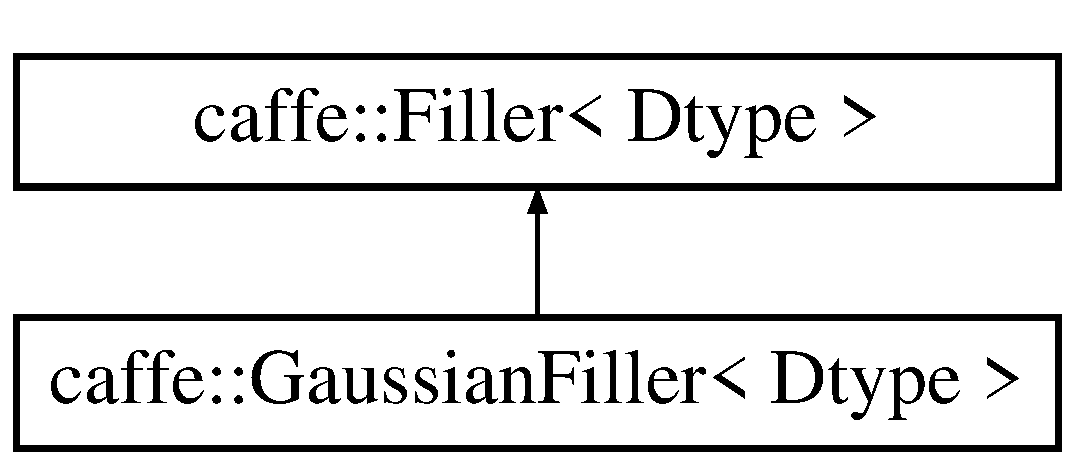
\includegraphics[height=2.000000cm]{classcaffe_1_1GaussianFiller}
\end{center}
\end{figure}
\subsection*{Public Member Functions}
\begin{DoxyCompactItemize}
\item 
{\bfseries Gaussian\+Filler} (const Filler\+Parameter \&param)\hypertarget{classcaffe_1_1GaussianFiller_a37a676739d64cf07b61767c99dd821b2}{}\label{classcaffe_1_1GaussianFiller_a37a676739d64cf07b61767c99dd821b2}

\item 
virtual void {\bfseries Fill} (\hyperlink{classcaffe_1_1Blob}{Blob}$<$ Dtype $>$ $\ast$blob)\hypertarget{classcaffe_1_1GaussianFiller_ac45d5d0695521d7d71a4d5bccb659f21}{}\label{classcaffe_1_1GaussianFiller_ac45d5d0695521d7d71a4d5bccb659f21}

\end{DoxyCompactItemize}
\subsection*{Protected Attributes}
\begin{DoxyCompactItemize}
\item 
shared\+\_\+ptr$<$ \hyperlink{classcaffe_1_1SyncedMemory}{Synced\+Memory} $>$ {\bfseries rand\+\_\+vec\+\_\+}\hypertarget{classcaffe_1_1GaussianFiller_afec462a3671a2ad0cc09b6149be0b63c}{}\label{classcaffe_1_1GaussianFiller_afec462a3671a2ad0cc09b6149be0b63c}

\end{DoxyCompactItemize}


\subsection{Detailed Description}
\subsubsection*{template$<$typename Dtype$>$\\*
class caffe\+::\+Gaussian\+Filler$<$ Dtype $>$}

Fills a \hyperlink{classcaffe_1_1Blob}{Blob} with Gaussian-\/distributed values $ x = a $. 

The documentation for this class was generated from the following file\+:\begin{DoxyCompactItemize}
\item 
include/caffe/filler.\+hpp\end{DoxyCompactItemize}

\hypertarget{classcaffe_1_1Caffe_1_1RNG_1_1Generator}{}\section{caffe\+:\+:Caffe\+:\+:R\+NG\+:\+:Generator Class Reference}
\label{classcaffe_1_1Caffe_1_1RNG_1_1Generator}\index{caffe\+::\+Caffe\+::\+R\+N\+G\+::\+Generator@{caffe\+::\+Caffe\+::\+R\+N\+G\+::\+Generator}}
\subsection*{Public Member Functions}
\begin{DoxyCompactItemize}
\item 
{\bfseries Generator} (unsigned int seed)\hypertarget{classcaffe_1_1Caffe_1_1RNG_1_1Generator_a25f41946ec93504bb7b132ef5072c0fc}{}\label{classcaffe_1_1Caffe_1_1RNG_1_1Generator_a25f41946ec93504bb7b132ef5072c0fc}

\item 
caffe\+::rng\+\_\+t $\ast$ {\bfseries rng} ()\hypertarget{classcaffe_1_1Caffe_1_1RNG_1_1Generator_a43c97cbef420858b7f611396cc5093bf}{}\label{classcaffe_1_1Caffe_1_1RNG_1_1Generator_a43c97cbef420858b7f611396cc5093bf}

\end{DoxyCompactItemize}


The documentation for this class was generated from the following file\+:\begin{DoxyCompactItemize}
\item 
src/caffe/common.\+cpp\end{DoxyCompactItemize}

\hypertarget{classcaffe_1_1HDF5DataLayer}{}\section{caffe\+:\+:H\+D\+F5\+Data\+Layer$<$ Dtype $>$ Class Template Reference}
\label{classcaffe_1_1HDF5DataLayer}\index{caffe\+::\+H\+D\+F5\+Data\+Layer$<$ Dtype $>$@{caffe\+::\+H\+D\+F5\+Data\+Layer$<$ Dtype $>$}}


Provides data to the \hyperlink{classcaffe_1_1Net}{Net} from H\+D\+F5 files.  




{\ttfamily \#include $<$hdf5\+\_\+data\+\_\+layer.\+hpp$>$}

Inheritance diagram for caffe\+:\+:H\+D\+F5\+Data\+Layer$<$ Dtype $>$\+:\begin{figure}[H]
\begin{center}
\leavevmode
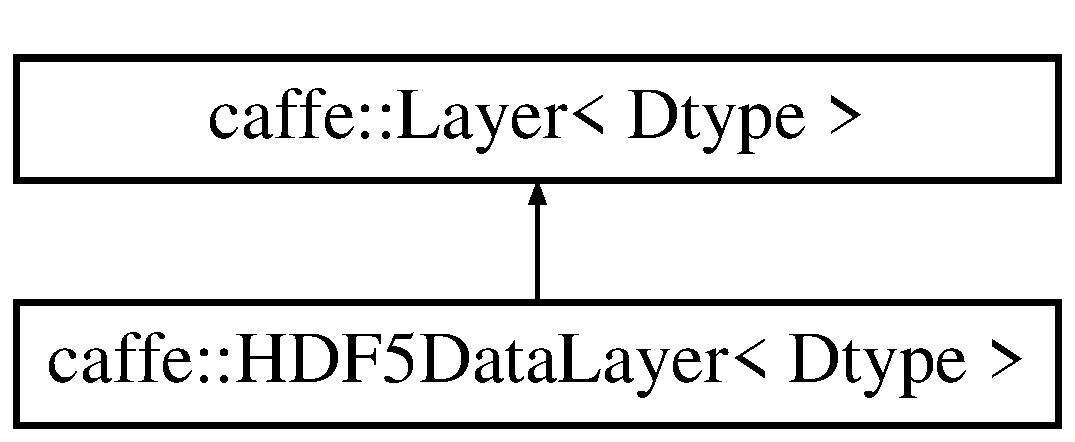
\includegraphics[height=2.000000cm]{classcaffe_1_1HDF5DataLayer}
\end{center}
\end{figure}
\subsection*{Public Member Functions}
\begin{DoxyCompactItemize}
\item 
{\bfseries H\+D\+F5\+Data\+Layer} (const Layer\+Parameter \&param)\hypertarget{classcaffe_1_1HDF5DataLayer_abfc7dcc4f07c228eb0deb1e0dfae1a5f}{}\label{classcaffe_1_1HDF5DataLayer_abfc7dcc4f07c228eb0deb1e0dfae1a5f}

\item 
virtual void \hyperlink{classcaffe_1_1HDF5DataLayer_a2422001e2f11da551cd4a4f7d3b43083}{Layer\+Set\+Up} (const vector$<$ \hyperlink{classcaffe_1_1Blob}{Blob}$<$ Dtype $>$ $\ast$ $>$ \&bottom, const vector$<$ \hyperlink{classcaffe_1_1Blob}{Blob}$<$ Dtype $>$ $\ast$ $>$ \&top)
\begin{DoxyCompactList}\small\item\em Does layer-\/specific setup\+: your layer should implement this function as well as Reshape. \end{DoxyCompactList}\item 
virtual void \hyperlink{classcaffe_1_1HDF5DataLayer_a5f036a0ee6132104ee6f1bfe2850fbcd}{Reshape} (const vector$<$ \hyperlink{classcaffe_1_1Blob}{Blob}$<$ Dtype $>$ $\ast$ $>$ \&bottom, const vector$<$ \hyperlink{classcaffe_1_1Blob}{Blob}$<$ Dtype $>$ $\ast$ $>$ \&top)
\begin{DoxyCompactList}\small\item\em Adjust the shapes of top blobs and internal buffers to accommodate the shapes of the bottom blobs. \end{DoxyCompactList}\item 
virtual const char $\ast$ \hyperlink{classcaffe_1_1HDF5DataLayer_af4e5df6d3dc0b342fe6eff3b1f7fd045}{type} () const \hypertarget{classcaffe_1_1HDF5DataLayer_af4e5df6d3dc0b342fe6eff3b1f7fd045}{}\label{classcaffe_1_1HDF5DataLayer_af4e5df6d3dc0b342fe6eff3b1f7fd045}

\begin{DoxyCompactList}\small\item\em Returns the layer type. \end{DoxyCompactList}\item 
virtual int \hyperlink{classcaffe_1_1HDF5DataLayer_a800a76c3afa9d5ac8042fa08d01b3bef}{Exact\+Num\+Bottom\+Blobs} () const 
\begin{DoxyCompactList}\small\item\em Returns the exact number of bottom blobs required by the layer, or -\/1 if no exact number is required. \end{DoxyCompactList}\item 
virtual int \hyperlink{classcaffe_1_1HDF5DataLayer_a5ee39cf7a1b4558811fe56bcec3c1fbe}{Min\+Top\+Blobs} () const 
\begin{DoxyCompactList}\small\item\em Returns the minimum number of top blobs required by the layer, or -\/1 if no minimum number is required. \end{DoxyCompactList}\end{DoxyCompactItemize}
\subsection*{Protected Member Functions}
\begin{DoxyCompactItemize}
\item 
void {\bfseries Next} ()\hypertarget{classcaffe_1_1HDF5DataLayer_a06dd19f9e75448e649bd6d1bdf628879}{}\label{classcaffe_1_1HDF5DataLayer_a06dd19f9e75448e649bd6d1bdf628879}

\item 
bool {\bfseries Skip} ()\hypertarget{classcaffe_1_1HDF5DataLayer_ad8fcb05eb70f5230d34b4dc1e641bc7b}{}\label{classcaffe_1_1HDF5DataLayer_ad8fcb05eb70f5230d34b4dc1e641bc7b}

\item 
virtual void \hyperlink{classcaffe_1_1HDF5DataLayer_ae95656f7e015d0df62fc20d848786034}{Forward\+\_\+cpu} (const vector$<$ \hyperlink{classcaffe_1_1Blob}{Blob}$<$ Dtype $>$ $\ast$ $>$ \&bottom, const vector$<$ \hyperlink{classcaffe_1_1Blob}{Blob}$<$ Dtype $>$ $\ast$ $>$ \&top)\hypertarget{classcaffe_1_1HDF5DataLayer_ae95656f7e015d0df62fc20d848786034}{}\label{classcaffe_1_1HDF5DataLayer_ae95656f7e015d0df62fc20d848786034}

\begin{DoxyCompactList}\small\item\em Using the C\+PU device, compute the layer output. \end{DoxyCompactList}\item 
virtual void \hyperlink{classcaffe_1_1HDF5DataLayer_a5732f15bc27b14bd2ba09413e05385db}{Forward\+\_\+gpu} (const vector$<$ \hyperlink{classcaffe_1_1Blob}{Blob}$<$ Dtype $>$ $\ast$ $>$ \&bottom, const vector$<$ \hyperlink{classcaffe_1_1Blob}{Blob}$<$ Dtype $>$ $\ast$ $>$ \&top)\hypertarget{classcaffe_1_1HDF5DataLayer_a5732f15bc27b14bd2ba09413e05385db}{}\label{classcaffe_1_1HDF5DataLayer_a5732f15bc27b14bd2ba09413e05385db}

\begin{DoxyCompactList}\small\item\em Using the G\+PU device, compute the layer output. Fall back to \hyperlink{classcaffe_1_1HDF5DataLayer_ae95656f7e015d0df62fc20d848786034}{Forward\+\_\+cpu()} if unavailable. \end{DoxyCompactList}\item 
virtual void \hyperlink{classcaffe_1_1HDF5DataLayer_a7239ed842b4e80c3bdf2b006eecde34a}{Backward\+\_\+cpu} (const vector$<$ \hyperlink{classcaffe_1_1Blob}{Blob}$<$ Dtype $>$ $\ast$ $>$ \&top, const vector$<$ bool $>$ \&propagate\+\_\+down, const vector$<$ \hyperlink{classcaffe_1_1Blob}{Blob}$<$ Dtype $>$ $\ast$ $>$ \&bottom)\hypertarget{classcaffe_1_1HDF5DataLayer_a7239ed842b4e80c3bdf2b006eecde34a}{}\label{classcaffe_1_1HDF5DataLayer_a7239ed842b4e80c3bdf2b006eecde34a}

\begin{DoxyCompactList}\small\item\em Using the C\+PU device, compute the gradients for any parameters and for the bottom blobs if propagate\+\_\+down is true. \end{DoxyCompactList}\item 
virtual void \hyperlink{classcaffe_1_1HDF5DataLayer_a052510a9ac8df9da59cefcacaecf07ce}{Backward\+\_\+gpu} (const vector$<$ \hyperlink{classcaffe_1_1Blob}{Blob}$<$ Dtype $>$ $\ast$ $>$ \&top, const vector$<$ bool $>$ \&propagate\+\_\+down, const vector$<$ \hyperlink{classcaffe_1_1Blob}{Blob}$<$ Dtype $>$ $\ast$ $>$ \&bottom)\hypertarget{classcaffe_1_1HDF5DataLayer_a052510a9ac8df9da59cefcacaecf07ce}{}\label{classcaffe_1_1HDF5DataLayer_a052510a9ac8df9da59cefcacaecf07ce}

\begin{DoxyCompactList}\small\item\em Using the G\+PU device, compute the gradients for any parameters and for the bottom blobs if propagate\+\_\+down is true. Fall back to \hyperlink{classcaffe_1_1HDF5DataLayer_a7239ed842b4e80c3bdf2b006eecde34a}{Backward\+\_\+cpu()} if unavailable. \end{DoxyCompactList}\item 
virtual void {\bfseries Load\+H\+D\+F5\+File\+Data} (const char $\ast$filename)\hypertarget{classcaffe_1_1HDF5DataLayer_a6fe59cc631f26f3323641ea480352119}{}\label{classcaffe_1_1HDF5DataLayer_a6fe59cc631f26f3323641ea480352119}

\end{DoxyCompactItemize}
\subsection*{Protected Attributes}
\begin{DoxyCompactItemize}
\item 
std\+::vector$<$ std\+::string $>$ {\bfseries hdf\+\_\+filenames\+\_\+}\hypertarget{classcaffe_1_1HDF5DataLayer_ae255f1e97fc8140bfeb7e3325f431f5a}{}\label{classcaffe_1_1HDF5DataLayer_ae255f1e97fc8140bfeb7e3325f431f5a}

\item 
unsigned int {\bfseries num\+\_\+files\+\_\+}\hypertarget{classcaffe_1_1HDF5DataLayer_aa6154c78cd3f375f1bba8dc544362e59}{}\label{classcaffe_1_1HDF5DataLayer_aa6154c78cd3f375f1bba8dc544362e59}

\item 
unsigned int {\bfseries current\+\_\+file\+\_\+}\hypertarget{classcaffe_1_1HDF5DataLayer_aa13b2e2012927eb433d007eb0cfcf8a7}{}\label{classcaffe_1_1HDF5DataLayer_aa13b2e2012927eb433d007eb0cfcf8a7}

\item 
hsize\+\_\+t {\bfseries current\+\_\+row\+\_\+}\hypertarget{classcaffe_1_1HDF5DataLayer_a375f447a432bcd2ba94859b5b270ac96}{}\label{classcaffe_1_1HDF5DataLayer_a375f447a432bcd2ba94859b5b270ac96}

\item 
std\+::vector$<$ shared\+\_\+ptr$<$ \hyperlink{classcaffe_1_1Blob}{Blob}$<$ Dtype $>$ $>$ $>$ {\bfseries hdf\+\_\+blobs\+\_\+}\hypertarget{classcaffe_1_1HDF5DataLayer_ac1978a2bb6dbcd7343bc13ee032328e3}{}\label{classcaffe_1_1HDF5DataLayer_ac1978a2bb6dbcd7343bc13ee032328e3}

\item 
std\+::vector$<$ unsigned int $>$ {\bfseries data\+\_\+permutation\+\_\+}\hypertarget{classcaffe_1_1HDF5DataLayer_a4b8ac8123356205c95dde2b7cd19835a}{}\label{classcaffe_1_1HDF5DataLayer_a4b8ac8123356205c95dde2b7cd19835a}

\item 
std\+::vector$<$ unsigned int $>$ {\bfseries file\+\_\+permutation\+\_\+}\hypertarget{classcaffe_1_1HDF5DataLayer_a9904d3326b0d687854b7aa62233d2f2f}{}\label{classcaffe_1_1HDF5DataLayer_a9904d3326b0d687854b7aa62233d2f2f}

\item 
uint64\+\_\+t {\bfseries offset\+\_\+}\hypertarget{classcaffe_1_1HDF5DataLayer_aa760969e3d444656b8dd4de2a2af1abe}{}\label{classcaffe_1_1HDF5DataLayer_aa760969e3d444656b8dd4de2a2af1abe}

\end{DoxyCompactItemize}


\subsection{Detailed Description}
\subsubsection*{template$<$typename Dtype$>$\\*
class caffe\+::\+H\+D\+F5\+Data\+Layer$<$ Dtype $>$}

Provides data to the \hyperlink{classcaffe_1_1Net}{Net} from H\+D\+F5 files. 

T\+O\+D\+O(dox)\+: thorough documentation for Forward and proto params. 

\subsection{Member Function Documentation}
\index{caffe\+::\+H\+D\+F5\+Data\+Layer@{caffe\+::\+H\+D\+F5\+Data\+Layer}!Exact\+Num\+Bottom\+Blobs@{Exact\+Num\+Bottom\+Blobs}}
\index{Exact\+Num\+Bottom\+Blobs@{Exact\+Num\+Bottom\+Blobs}!caffe\+::\+H\+D\+F5\+Data\+Layer@{caffe\+::\+H\+D\+F5\+Data\+Layer}}
\subsubsection[{\texorpdfstring{Exact\+Num\+Bottom\+Blobs() const }{ExactNumBottomBlobs() const }}]{\setlength{\rightskip}{0pt plus 5cm}template$<$typename Dtype $>$ virtual int {\bf caffe\+::\+H\+D\+F5\+Data\+Layer}$<$ Dtype $>$\+::Exact\+Num\+Bottom\+Blobs (
\begin{DoxyParamCaption}
{}
\end{DoxyParamCaption}
) const\hspace{0.3cm}{\ttfamily [inline]}, {\ttfamily [virtual]}}\hypertarget{classcaffe_1_1HDF5DataLayer_a800a76c3afa9d5ac8042fa08d01b3bef}{}\label{classcaffe_1_1HDF5DataLayer_a800a76c3afa9d5ac8042fa08d01b3bef}


Returns the exact number of bottom blobs required by the layer, or -\/1 if no exact number is required. 

This method should be overridden to return a non-\/negative value if your layer expects some exact number of bottom blobs. 

Reimplemented from \hyperlink{classcaffe_1_1Layer_a45c7a7943a8a6735ac433c9be11e0240}{caffe\+::\+Layer$<$ Dtype $>$}.

\index{caffe\+::\+H\+D\+F5\+Data\+Layer@{caffe\+::\+H\+D\+F5\+Data\+Layer}!Layer\+Set\+Up@{Layer\+Set\+Up}}
\index{Layer\+Set\+Up@{Layer\+Set\+Up}!caffe\+::\+H\+D\+F5\+Data\+Layer@{caffe\+::\+H\+D\+F5\+Data\+Layer}}
\subsubsection[{\texorpdfstring{Layer\+Set\+Up(const vector$<$ Blob$<$ Dtype $>$ $\ast$ $>$ \&bottom, const vector$<$ Blob$<$ Dtype $>$ $\ast$ $>$ \&top)}{LayerSetUp(const vector< Blob< Dtype > * > &bottom, const vector< Blob< Dtype > * > &top)}}]{\setlength{\rightskip}{0pt plus 5cm}template$<$typename Dtype $>$ void {\bf caffe\+::\+H\+D\+F5\+Data\+Layer}$<$ Dtype $>$\+::Layer\+Set\+Up (
\begin{DoxyParamCaption}
\item[{const vector$<$ {\bf Blob}$<$ Dtype $>$ $\ast$ $>$ \&}]{bottom, }
\item[{const vector$<$ {\bf Blob}$<$ Dtype $>$ $\ast$ $>$ \&}]{top}
\end{DoxyParamCaption}
)\hspace{0.3cm}{\ttfamily [virtual]}}\hypertarget{classcaffe_1_1HDF5DataLayer_a2422001e2f11da551cd4a4f7d3b43083}{}\label{classcaffe_1_1HDF5DataLayer_a2422001e2f11da551cd4a4f7d3b43083}


Does layer-\/specific setup\+: your layer should implement this function as well as Reshape. 


\begin{DoxyParams}{Parameters}
{\em bottom} & the preshaped input blobs, whose data fields store the input data for this layer \\
\hline
{\em top} & the allocated but unshaped output blobs\\
\hline
\end{DoxyParams}
This method should do one-\/time layer specific setup. This includes reading and processing relevent parameters from the {\ttfamily layer\+\_\+param\+\_\+}. Setting up the shapes of top blobs and internal buffers should be done in {\ttfamily Reshape}, which will be called before the forward pass to adjust the top blob sizes. 

Reimplemented from \hyperlink{classcaffe_1_1Layer_a38dc2488bf319b8de5a7ac84e0045393}{caffe\+::\+Layer$<$ Dtype $>$}.

\index{caffe\+::\+H\+D\+F5\+Data\+Layer@{caffe\+::\+H\+D\+F5\+Data\+Layer}!Min\+Top\+Blobs@{Min\+Top\+Blobs}}
\index{Min\+Top\+Blobs@{Min\+Top\+Blobs}!caffe\+::\+H\+D\+F5\+Data\+Layer@{caffe\+::\+H\+D\+F5\+Data\+Layer}}
\subsubsection[{\texorpdfstring{Min\+Top\+Blobs() const }{MinTopBlobs() const }}]{\setlength{\rightskip}{0pt plus 5cm}template$<$typename Dtype $>$ virtual int {\bf caffe\+::\+H\+D\+F5\+Data\+Layer}$<$ Dtype $>$\+::Min\+Top\+Blobs (
\begin{DoxyParamCaption}
{}
\end{DoxyParamCaption}
) const\hspace{0.3cm}{\ttfamily [inline]}, {\ttfamily [virtual]}}\hypertarget{classcaffe_1_1HDF5DataLayer_a5ee39cf7a1b4558811fe56bcec3c1fbe}{}\label{classcaffe_1_1HDF5DataLayer_a5ee39cf7a1b4558811fe56bcec3c1fbe}


Returns the minimum number of top blobs required by the layer, or -\/1 if no minimum number is required. 

This method should be overridden to return a non-\/negative value if your layer expects some minimum number of top blobs. 

Reimplemented from \hyperlink{classcaffe_1_1Layer_a8bb143d58a740345fa2dc3d4204d553b}{caffe\+::\+Layer$<$ Dtype $>$}.

\index{caffe\+::\+H\+D\+F5\+Data\+Layer@{caffe\+::\+H\+D\+F5\+Data\+Layer}!Reshape@{Reshape}}
\index{Reshape@{Reshape}!caffe\+::\+H\+D\+F5\+Data\+Layer@{caffe\+::\+H\+D\+F5\+Data\+Layer}}
\subsubsection[{\texorpdfstring{Reshape(const vector$<$ Blob$<$ Dtype $>$ $\ast$ $>$ \&bottom, const vector$<$ Blob$<$ Dtype $>$ $\ast$ $>$ \&top)}{Reshape(const vector< Blob< Dtype > * > &bottom, const vector< Blob< Dtype > * > &top)}}]{\setlength{\rightskip}{0pt plus 5cm}template$<$typename Dtype $>$ virtual void {\bf caffe\+::\+H\+D\+F5\+Data\+Layer}$<$ Dtype $>$\+::Reshape (
\begin{DoxyParamCaption}
\item[{const vector$<$ {\bf Blob}$<$ Dtype $>$ $\ast$ $>$ \&}]{bottom, }
\item[{const vector$<$ {\bf Blob}$<$ Dtype $>$ $\ast$ $>$ \&}]{top}
\end{DoxyParamCaption}
)\hspace{0.3cm}{\ttfamily [inline]}, {\ttfamily [virtual]}}\hypertarget{classcaffe_1_1HDF5DataLayer_a5f036a0ee6132104ee6f1bfe2850fbcd}{}\label{classcaffe_1_1HDF5DataLayer_a5f036a0ee6132104ee6f1bfe2850fbcd}


Adjust the shapes of top blobs and internal buffers to accommodate the shapes of the bottom blobs. 


\begin{DoxyParams}{Parameters}
{\em bottom} & the input blobs, with the requested input shapes \\
\hline
{\em top} & the top blobs, which should be reshaped as needed\\
\hline
\end{DoxyParams}
This method should reshape top blobs as needed according to the shapes of the bottom (input) blobs, as well as reshaping any internal buffers and making any other necessary adjustments so that the layer can accommodate the bottom blobs. 

Implements \hyperlink{classcaffe_1_1Layer_ad9d391b972c769c0ebee34ca6d1c973e}{caffe\+::\+Layer$<$ Dtype $>$}.



The documentation for this class was generated from the following files\+:\begin{DoxyCompactItemize}
\item 
include/caffe/layers/hdf5\+\_\+data\+\_\+layer.\+hpp\item 
src/caffe/layers/hdf5\+\_\+data\+\_\+layer.\+cpp\end{DoxyCompactItemize}

\hypertarget{classcaffe_1_1HDF5OutputLayer}{}\section{caffe\+:\+:H\+D\+F5\+Output\+Layer$<$ Dtype $>$ Class Template Reference}
\label{classcaffe_1_1HDF5OutputLayer}\index{caffe\+::\+H\+D\+F5\+Output\+Layer$<$ Dtype $>$@{caffe\+::\+H\+D\+F5\+Output\+Layer$<$ Dtype $>$}}


Write blobs to disk as H\+D\+F5 files.  




{\ttfamily \#include $<$hdf5\+\_\+output\+\_\+layer.\+hpp$>$}

Inheritance diagram for caffe\+:\+:H\+D\+F5\+Output\+Layer$<$ Dtype $>$\+:\begin{figure}[H]
\begin{center}
\leavevmode
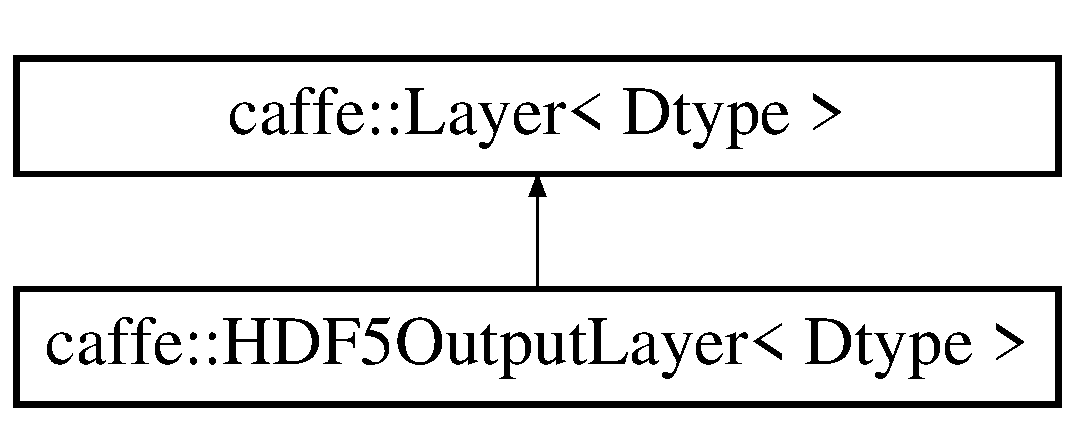
\includegraphics[height=2.000000cm]{classcaffe_1_1HDF5OutputLayer}
\end{center}
\end{figure}
\subsection*{Public Member Functions}
\begin{DoxyCompactItemize}
\item 
{\bfseries H\+D\+F5\+Output\+Layer} (const Layer\+Parameter \&param)\hypertarget{classcaffe_1_1HDF5OutputLayer_acf9e02d15a72cb6838e8fd2860e046b5}{}\label{classcaffe_1_1HDF5OutputLayer_acf9e02d15a72cb6838e8fd2860e046b5}

\item 
virtual void \hyperlink{classcaffe_1_1HDF5OutputLayer_a50777ff487cdca409c912af31d36b499}{Layer\+Set\+Up} (const vector$<$ \hyperlink{classcaffe_1_1Blob}{Blob}$<$ Dtype $>$ $\ast$ $>$ \&bottom, const vector$<$ \hyperlink{classcaffe_1_1Blob}{Blob}$<$ Dtype $>$ $\ast$ $>$ \&top)
\begin{DoxyCompactList}\small\item\em Does layer-\/specific setup\+: your layer should implement this function as well as Reshape. \end{DoxyCompactList}\item 
virtual void \hyperlink{classcaffe_1_1HDF5OutputLayer_ad0478aa253430dfc405336f98264f8c5}{Reshape} (const vector$<$ \hyperlink{classcaffe_1_1Blob}{Blob}$<$ Dtype $>$ $\ast$ $>$ \&bottom, const vector$<$ \hyperlink{classcaffe_1_1Blob}{Blob}$<$ Dtype $>$ $\ast$ $>$ \&top)
\begin{DoxyCompactList}\small\item\em Adjust the shapes of top blobs and internal buffers to accommodate the shapes of the bottom blobs. \end{DoxyCompactList}\item 
virtual const char $\ast$ \hyperlink{classcaffe_1_1HDF5OutputLayer_a01427fa792250df062b97460175cadfb}{type} () const \hypertarget{classcaffe_1_1HDF5OutputLayer_a01427fa792250df062b97460175cadfb}{}\label{classcaffe_1_1HDF5OutputLayer_a01427fa792250df062b97460175cadfb}

\begin{DoxyCompactList}\small\item\em Returns the layer type. \end{DoxyCompactList}\item 
virtual int \hyperlink{classcaffe_1_1HDF5OutputLayer_af874ff0bf8f1817f44d18398889bcbe4}{Exact\+Num\+Bottom\+Blobs} () const 
\begin{DoxyCompactList}\small\item\em Returns the exact number of bottom blobs required by the layer, or -\/1 if no exact number is required. \end{DoxyCompactList}\item 
virtual int \hyperlink{classcaffe_1_1HDF5OutputLayer_a2c754adb8c37b1299507865fdb616149}{Exact\+Num\+Top\+Blobs} () const 
\begin{DoxyCompactList}\small\item\em Returns the exact number of top blobs required by the layer, or -\/1 if no exact number is required. \end{DoxyCompactList}\item 
std\+::string {\bfseries file\+\_\+name} () const \hypertarget{classcaffe_1_1HDF5OutputLayer_aca8e3392384521de35e87618d3208571}{}\label{classcaffe_1_1HDF5OutputLayer_aca8e3392384521de35e87618d3208571}

\end{DoxyCompactItemize}
\subsection*{Protected Member Functions}
\begin{DoxyCompactItemize}
\item 
virtual void \hyperlink{classcaffe_1_1HDF5OutputLayer_a5b2e57b3d6bfad113a608df5e8a49c26}{Forward\+\_\+cpu} (const vector$<$ \hyperlink{classcaffe_1_1Blob}{Blob}$<$ Dtype $>$ $\ast$ $>$ \&bottom, const vector$<$ \hyperlink{classcaffe_1_1Blob}{Blob}$<$ Dtype $>$ $\ast$ $>$ \&top)\hypertarget{classcaffe_1_1HDF5OutputLayer_a5b2e57b3d6bfad113a608df5e8a49c26}{}\label{classcaffe_1_1HDF5OutputLayer_a5b2e57b3d6bfad113a608df5e8a49c26}

\begin{DoxyCompactList}\small\item\em Using the C\+PU device, compute the layer output. \end{DoxyCompactList}\item 
virtual void \hyperlink{classcaffe_1_1HDF5OutputLayer_a3843a210cfc93626f28f2fd71be2b6b6}{Forward\+\_\+gpu} (const vector$<$ \hyperlink{classcaffe_1_1Blob}{Blob}$<$ Dtype $>$ $\ast$ $>$ \&bottom, const vector$<$ \hyperlink{classcaffe_1_1Blob}{Blob}$<$ Dtype $>$ $\ast$ $>$ \&top)\hypertarget{classcaffe_1_1HDF5OutputLayer_a3843a210cfc93626f28f2fd71be2b6b6}{}\label{classcaffe_1_1HDF5OutputLayer_a3843a210cfc93626f28f2fd71be2b6b6}

\begin{DoxyCompactList}\small\item\em Using the G\+PU device, compute the layer output. Fall back to \hyperlink{classcaffe_1_1HDF5OutputLayer_a5b2e57b3d6bfad113a608df5e8a49c26}{Forward\+\_\+cpu()} if unavailable. \end{DoxyCompactList}\item 
virtual void \hyperlink{classcaffe_1_1HDF5OutputLayer_aaf5106f73266c501ebbb231df988f52a}{Backward\+\_\+cpu} (const vector$<$ \hyperlink{classcaffe_1_1Blob}{Blob}$<$ Dtype $>$ $\ast$ $>$ \&top, const vector$<$ bool $>$ \&propagate\+\_\+down, const vector$<$ \hyperlink{classcaffe_1_1Blob}{Blob}$<$ Dtype $>$ $\ast$ $>$ \&bottom)\hypertarget{classcaffe_1_1HDF5OutputLayer_aaf5106f73266c501ebbb231df988f52a}{}\label{classcaffe_1_1HDF5OutputLayer_aaf5106f73266c501ebbb231df988f52a}

\begin{DoxyCompactList}\small\item\em Using the C\+PU device, compute the gradients for any parameters and for the bottom blobs if propagate\+\_\+down is true. \end{DoxyCompactList}\item 
virtual void \hyperlink{classcaffe_1_1HDF5OutputLayer_a35cc8c1e4feb64896300bbfd157668f0}{Backward\+\_\+gpu} (const vector$<$ \hyperlink{classcaffe_1_1Blob}{Blob}$<$ Dtype $>$ $\ast$ $>$ \&top, const vector$<$ bool $>$ \&propagate\+\_\+down, const vector$<$ \hyperlink{classcaffe_1_1Blob}{Blob}$<$ Dtype $>$ $\ast$ $>$ \&bottom)\hypertarget{classcaffe_1_1HDF5OutputLayer_a35cc8c1e4feb64896300bbfd157668f0}{}\label{classcaffe_1_1HDF5OutputLayer_a35cc8c1e4feb64896300bbfd157668f0}

\begin{DoxyCompactList}\small\item\em Using the G\+PU device, compute the gradients for any parameters and for the bottom blobs if propagate\+\_\+down is true. Fall back to \hyperlink{classcaffe_1_1HDF5OutputLayer_aaf5106f73266c501ebbb231df988f52a}{Backward\+\_\+cpu()} if unavailable. \end{DoxyCompactList}\item 
virtual void {\bfseries Save\+Blobs} ()\hypertarget{classcaffe_1_1HDF5OutputLayer_a56c7ba8e69d0867d550dddd928863a2f}{}\label{classcaffe_1_1HDF5OutputLayer_a56c7ba8e69d0867d550dddd928863a2f}

\end{DoxyCompactItemize}
\subsection*{Protected Attributes}
\begin{DoxyCompactItemize}
\item 
bool {\bfseries file\+\_\+opened\+\_\+}\hypertarget{classcaffe_1_1HDF5OutputLayer_a995b7eadf9ccd19c02a7f54ee3dd97c2}{}\label{classcaffe_1_1HDF5OutputLayer_a995b7eadf9ccd19c02a7f54ee3dd97c2}

\item 
std\+::string {\bfseries file\+\_\+name\+\_\+}\hypertarget{classcaffe_1_1HDF5OutputLayer_aa4609affd7a57ba7481b98afed3f7985}{}\label{classcaffe_1_1HDF5OutputLayer_aa4609affd7a57ba7481b98afed3f7985}

\item 
hid\+\_\+t {\bfseries file\+\_\+id\+\_\+}\hypertarget{classcaffe_1_1HDF5OutputLayer_a353a5e36b3baa08e381dc5da1bb8b74e}{}\label{classcaffe_1_1HDF5OutputLayer_a353a5e36b3baa08e381dc5da1bb8b74e}

\item 
\hyperlink{classcaffe_1_1Blob}{Blob}$<$ Dtype $>$ {\bfseries data\+\_\+blob\+\_\+}\hypertarget{classcaffe_1_1HDF5OutputLayer_ad91a29d84d4f7c577adf1b634fec1d92}{}\label{classcaffe_1_1HDF5OutputLayer_ad91a29d84d4f7c577adf1b634fec1d92}

\item 
\hyperlink{classcaffe_1_1Blob}{Blob}$<$ Dtype $>$ {\bfseries label\+\_\+blob\+\_\+}\hypertarget{classcaffe_1_1HDF5OutputLayer_aef72be0097ab1894a5414b74512e3807}{}\label{classcaffe_1_1HDF5OutputLayer_aef72be0097ab1894a5414b74512e3807}

\end{DoxyCompactItemize}


\subsection{Detailed Description}
\subsubsection*{template$<$typename Dtype$>$\\*
class caffe\+::\+H\+D\+F5\+Output\+Layer$<$ Dtype $>$}

Write blobs to disk as H\+D\+F5 files. 

T\+O\+D\+O(dox)\+: thorough documentation for Forward and proto params. 

\subsection{Member Function Documentation}
\index{caffe\+::\+H\+D\+F5\+Output\+Layer@{caffe\+::\+H\+D\+F5\+Output\+Layer}!Exact\+Num\+Bottom\+Blobs@{Exact\+Num\+Bottom\+Blobs}}
\index{Exact\+Num\+Bottom\+Blobs@{Exact\+Num\+Bottom\+Blobs}!caffe\+::\+H\+D\+F5\+Output\+Layer@{caffe\+::\+H\+D\+F5\+Output\+Layer}}
\subsubsection[{\texorpdfstring{Exact\+Num\+Bottom\+Blobs() const }{ExactNumBottomBlobs() const }}]{\setlength{\rightskip}{0pt plus 5cm}template$<$typename Dtype $>$ virtual int {\bf caffe\+::\+H\+D\+F5\+Output\+Layer}$<$ Dtype $>$\+::Exact\+Num\+Bottom\+Blobs (
\begin{DoxyParamCaption}
{}
\end{DoxyParamCaption}
) const\hspace{0.3cm}{\ttfamily [inline]}, {\ttfamily [virtual]}}\hypertarget{classcaffe_1_1HDF5OutputLayer_af874ff0bf8f1817f44d18398889bcbe4}{}\label{classcaffe_1_1HDF5OutputLayer_af874ff0bf8f1817f44d18398889bcbe4}


Returns the exact number of bottom blobs required by the layer, or -\/1 if no exact number is required. 

This method should be overridden to return a non-\/negative value if your layer expects some exact number of bottom blobs. 

Reimplemented from \hyperlink{classcaffe_1_1Layer_a45c7a7943a8a6735ac433c9be11e0240}{caffe\+::\+Layer$<$ Dtype $>$}.

\index{caffe\+::\+H\+D\+F5\+Output\+Layer@{caffe\+::\+H\+D\+F5\+Output\+Layer}!Exact\+Num\+Top\+Blobs@{Exact\+Num\+Top\+Blobs}}
\index{Exact\+Num\+Top\+Blobs@{Exact\+Num\+Top\+Blobs}!caffe\+::\+H\+D\+F5\+Output\+Layer@{caffe\+::\+H\+D\+F5\+Output\+Layer}}
\subsubsection[{\texorpdfstring{Exact\+Num\+Top\+Blobs() const }{ExactNumTopBlobs() const }}]{\setlength{\rightskip}{0pt plus 5cm}template$<$typename Dtype $>$ virtual int {\bf caffe\+::\+H\+D\+F5\+Output\+Layer}$<$ Dtype $>$\+::Exact\+Num\+Top\+Blobs (
\begin{DoxyParamCaption}
{}
\end{DoxyParamCaption}
) const\hspace{0.3cm}{\ttfamily [inline]}, {\ttfamily [virtual]}}\hypertarget{classcaffe_1_1HDF5OutputLayer_a2c754adb8c37b1299507865fdb616149}{}\label{classcaffe_1_1HDF5OutputLayer_a2c754adb8c37b1299507865fdb616149}


Returns the exact number of top blobs required by the layer, or -\/1 if no exact number is required. 

This method should be overridden to return a non-\/negative value if your layer expects some exact number of top blobs. 

Reimplemented from \hyperlink{classcaffe_1_1Layer_aa3c99ed707e8db683a3043412e151af8}{caffe\+::\+Layer$<$ Dtype $>$}.

\index{caffe\+::\+H\+D\+F5\+Output\+Layer@{caffe\+::\+H\+D\+F5\+Output\+Layer}!Layer\+Set\+Up@{Layer\+Set\+Up}}
\index{Layer\+Set\+Up@{Layer\+Set\+Up}!caffe\+::\+H\+D\+F5\+Output\+Layer@{caffe\+::\+H\+D\+F5\+Output\+Layer}}
\subsubsection[{\texorpdfstring{Layer\+Set\+Up(const vector$<$ Blob$<$ Dtype $>$ $\ast$ $>$ \&bottom, const vector$<$ Blob$<$ Dtype $>$ $\ast$ $>$ \&top)}{LayerSetUp(const vector< Blob< Dtype > * > &bottom, const vector< Blob< Dtype > * > &top)}}]{\setlength{\rightskip}{0pt plus 5cm}template$<$typename Dtype $>$ void {\bf caffe\+::\+H\+D\+F5\+Output\+Layer}$<$ Dtype $>$\+::Layer\+Set\+Up (
\begin{DoxyParamCaption}
\item[{const vector$<$ {\bf Blob}$<$ Dtype $>$ $\ast$ $>$ \&}]{bottom, }
\item[{const vector$<$ {\bf Blob}$<$ Dtype $>$ $\ast$ $>$ \&}]{top}
\end{DoxyParamCaption}
)\hspace{0.3cm}{\ttfamily [virtual]}}\hypertarget{classcaffe_1_1HDF5OutputLayer_a50777ff487cdca409c912af31d36b499}{}\label{classcaffe_1_1HDF5OutputLayer_a50777ff487cdca409c912af31d36b499}


Does layer-\/specific setup\+: your layer should implement this function as well as Reshape. 


\begin{DoxyParams}{Parameters}
{\em bottom} & the preshaped input blobs, whose data fields store the input data for this layer \\
\hline
{\em top} & the allocated but unshaped output blobs\\
\hline
\end{DoxyParams}
This method should do one-\/time layer specific setup. This includes reading and processing relevent parameters from the {\ttfamily layer\+\_\+param\+\_\+}. Setting up the shapes of top blobs and internal buffers should be done in {\ttfamily Reshape}, which will be called before the forward pass to adjust the top blob sizes. 

Reimplemented from \hyperlink{classcaffe_1_1Layer_a38dc2488bf319b8de5a7ac84e0045393}{caffe\+::\+Layer$<$ Dtype $>$}.

\index{caffe\+::\+H\+D\+F5\+Output\+Layer@{caffe\+::\+H\+D\+F5\+Output\+Layer}!Reshape@{Reshape}}
\index{Reshape@{Reshape}!caffe\+::\+H\+D\+F5\+Output\+Layer@{caffe\+::\+H\+D\+F5\+Output\+Layer}}
\subsubsection[{\texorpdfstring{Reshape(const vector$<$ Blob$<$ Dtype $>$ $\ast$ $>$ \&bottom, const vector$<$ Blob$<$ Dtype $>$ $\ast$ $>$ \&top)}{Reshape(const vector< Blob< Dtype > * > &bottom, const vector< Blob< Dtype > * > &top)}}]{\setlength{\rightskip}{0pt plus 5cm}template$<$typename Dtype $>$ virtual void {\bf caffe\+::\+H\+D\+F5\+Output\+Layer}$<$ Dtype $>$\+::Reshape (
\begin{DoxyParamCaption}
\item[{const vector$<$ {\bf Blob}$<$ Dtype $>$ $\ast$ $>$ \&}]{bottom, }
\item[{const vector$<$ {\bf Blob}$<$ Dtype $>$ $\ast$ $>$ \&}]{top}
\end{DoxyParamCaption}
)\hspace{0.3cm}{\ttfamily [inline]}, {\ttfamily [virtual]}}\hypertarget{classcaffe_1_1HDF5OutputLayer_ad0478aa253430dfc405336f98264f8c5}{}\label{classcaffe_1_1HDF5OutputLayer_ad0478aa253430dfc405336f98264f8c5}


Adjust the shapes of top blobs and internal buffers to accommodate the shapes of the bottom blobs. 


\begin{DoxyParams}{Parameters}
{\em bottom} & the input blobs, with the requested input shapes \\
\hline
{\em top} & the top blobs, which should be reshaped as needed\\
\hline
\end{DoxyParams}
This method should reshape top blobs as needed according to the shapes of the bottom (input) blobs, as well as reshaping any internal buffers and making any other necessary adjustments so that the layer can accommodate the bottom blobs. 

Implements \hyperlink{classcaffe_1_1Layer_ad9d391b972c769c0ebee34ca6d1c973e}{caffe\+::\+Layer$<$ Dtype $>$}.



The documentation for this class was generated from the following files\+:\begin{DoxyCompactItemize}
\item 
include/caffe/layers/hdf5\+\_\+output\+\_\+layer.\+hpp\item 
src/caffe/layers/hdf5\+\_\+output\+\_\+layer.\+cpp\end{DoxyCompactItemize}

\hypertarget{classcaffe_1_1HingeLossLayer}{}\section{caffe\+:\+:Hinge\+Loss\+Layer$<$ Dtype $>$ Class Template Reference}
\label{classcaffe_1_1HingeLossLayer}\index{caffe\+::\+Hinge\+Loss\+Layer$<$ Dtype $>$@{caffe\+::\+Hinge\+Loss\+Layer$<$ Dtype $>$}}


Computes the hinge loss for a one-\/of-\/many classification task.  




{\ttfamily \#include $<$hinge\+\_\+loss\+\_\+layer.\+hpp$>$}

Inheritance diagram for caffe\+:\+:Hinge\+Loss\+Layer$<$ Dtype $>$\+:\begin{figure}[H]
\begin{center}
\leavevmode
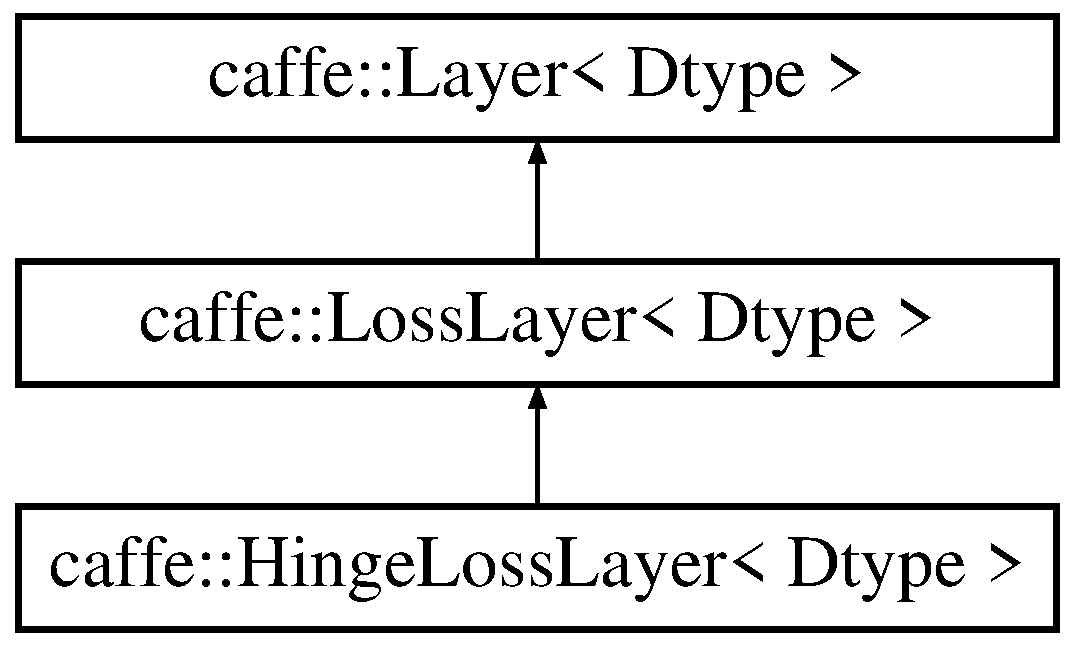
\includegraphics[height=3.000000cm]{classcaffe_1_1HingeLossLayer}
\end{center}
\end{figure}
\subsection*{Public Member Functions}
\begin{DoxyCompactItemize}
\item 
{\bfseries Hinge\+Loss\+Layer} (const Layer\+Parameter \&param)\hypertarget{classcaffe_1_1HingeLossLayer_a358a5bd2625bb7fed61052dd8e1cb588}{}\label{classcaffe_1_1HingeLossLayer_a358a5bd2625bb7fed61052dd8e1cb588}

\item 
virtual const char $\ast$ \hyperlink{classcaffe_1_1HingeLossLayer_ae804bb931e8cf835ac77a0529f89463f}{type} () const \hypertarget{classcaffe_1_1HingeLossLayer_ae804bb931e8cf835ac77a0529f89463f}{}\label{classcaffe_1_1HingeLossLayer_ae804bb931e8cf835ac77a0529f89463f}

\begin{DoxyCompactList}\small\item\em Returns the layer type. \end{DoxyCompactList}\end{DoxyCompactItemize}
\subsection*{Protected Member Functions}
\begin{DoxyCompactItemize}
\item 
virtual void \hyperlink{classcaffe_1_1HingeLossLayer_a24a8c6e0dca1b35794a14e5f923d226f}{Forward\+\_\+cpu} (const vector$<$ \hyperlink{classcaffe_1_1Blob}{Blob}$<$ Dtype $>$ $\ast$ $>$ \&bottom, const vector$<$ \hyperlink{classcaffe_1_1Blob}{Blob}$<$ Dtype $>$ $\ast$ $>$ \&top)
\begin{DoxyCompactList}\small\item\em Computes the hinge loss for a one-\/of-\/many classification task. \end{DoxyCompactList}\item 
virtual void \hyperlink{classcaffe_1_1HingeLossLayer_a24e8552d75a557b6082c197fd726412e}{Backward\+\_\+cpu} (const vector$<$ \hyperlink{classcaffe_1_1Blob}{Blob}$<$ Dtype $>$ $\ast$ $>$ \&top, const vector$<$ bool $>$ \&propagate\+\_\+down, const vector$<$ \hyperlink{classcaffe_1_1Blob}{Blob}$<$ Dtype $>$ $\ast$ $>$ \&bottom)
\begin{DoxyCompactList}\small\item\em Computes the hinge loss error gradient w.\+r.\+t. the predictions. \end{DoxyCompactList}\end{DoxyCompactItemize}
\subsection*{Additional Inherited Members}


\subsection{Detailed Description}
\subsubsection*{template$<$typename Dtype$>$\\*
class caffe\+::\+Hinge\+Loss\+Layer$<$ Dtype $>$}

Computes the hinge loss for a one-\/of-\/many classification task. 


\begin{DoxyParams}{Parameters}
{\em bottom} & input \hyperlink{classcaffe_1_1Blob}{Blob} vector (length 2)
\begin{DoxyEnumerate}
\item $ (N \times C \times H \times W) $ the predictions $ t $, a \hyperlink{classcaffe_1_1Blob}{Blob} with values in $ [-\infty, +\infty] $ indicating the predicted score for each of the $ K = CHW $ classes. In an S\+VM, $ t $ is the result of taking the inner product $ X^T W $ of the D-\/dimensional features $ X \in \mathcal{R}^{D \times N} $ and the learned hyperplane parameters $ W \in \mathcal{R}^{D \times K} $, so a \hyperlink{classcaffe_1_1Net}{Net} with just an \hyperlink{classcaffe_1_1InnerProductLayer}{Inner\+Product\+Layer} (with num\+\_\+output = D) providing predictions to a \hyperlink{classcaffe_1_1HingeLossLayer}{Hinge\+Loss\+Layer} and no other learnable parameters or losses is equivalent to an S\+VM.
\item $ (N \times 1 \times 1 \times 1) $ the labels $ l $, an integer-\/valued \hyperlink{classcaffe_1_1Blob}{Blob} with values $ l_n \in [0, 1, 2, ..., K - 1] $ indicating the correct class label among the $ K $ classes 
\end{DoxyEnumerate}\\
\hline
{\em top} & output \hyperlink{classcaffe_1_1Blob}{Blob} vector (length 1)
\begin{DoxyEnumerate}
\item $ (1 \times 1 \times 1 \times 1) $ the computed hinge loss\+: $ E = \frac{1}{N} \sum\limits_{n=1}^N \sum\limits_{k=1}^K [\max(0, 1 - \delta\{l_n = k\} t_{nk})] ^ p $, for the $ L^p $ norm (defaults to $ p = 1 $, the L1 norm; L2 norm, as in L2-\/\+S\+VM, is also available), and $ \delta\{\mathrm{condition}\} = \left\{ \begin{array}{lr} 1 & \mbox{if condition} \\ -1 & \mbox{otherwise} \end{array} \right. $
\end{DoxyEnumerate}\\
\hline
\end{DoxyParams}
In an S\+VM, $ t \in \mathcal{R}^{N \times K} $ is the result of taking the inner product $ X^T W $ of the features $ X \in \mathcal{R}^{D \times N} $ and the learned hyperplane parameters $ W \in \mathcal{R}^{D \times K} $. So, a \hyperlink{classcaffe_1_1Net}{Net} with just an \hyperlink{classcaffe_1_1InnerProductLayer}{Inner\+Product\+Layer} (with num\+\_\+output = $k$) providing predictions to a \hyperlink{classcaffe_1_1HingeLossLayer}{Hinge\+Loss\+Layer} is equivalent to an S\+VM (assuming it has no other learned outside the \hyperlink{classcaffe_1_1InnerProductLayer}{Inner\+Product\+Layer} and no other losses outside the \hyperlink{classcaffe_1_1HingeLossLayer}{Hinge\+Loss\+Layer}). 

\subsection{Member Function Documentation}
\index{caffe\+::\+Hinge\+Loss\+Layer@{caffe\+::\+Hinge\+Loss\+Layer}!Backward\+\_\+cpu@{Backward\+\_\+cpu}}
\index{Backward\+\_\+cpu@{Backward\+\_\+cpu}!caffe\+::\+Hinge\+Loss\+Layer@{caffe\+::\+Hinge\+Loss\+Layer}}
\subsubsection[{\texorpdfstring{Backward\+\_\+cpu(const vector$<$ Blob$<$ Dtype $>$ $\ast$ $>$ \&top, const vector$<$ bool $>$ \&propagate\+\_\+down, const vector$<$ Blob$<$ Dtype $>$ $\ast$ $>$ \&bottom)}{Backward_cpu(const vector< Blob< Dtype > * > &top, const vector< bool > &propagate_down, const vector< Blob< Dtype > * > &bottom)}}]{\setlength{\rightskip}{0pt plus 5cm}template$<$typename Dtype $>$ void {\bf caffe\+::\+Hinge\+Loss\+Layer}$<$ Dtype $>$\+::Backward\+\_\+cpu (
\begin{DoxyParamCaption}
\item[{const vector$<$ {\bf Blob}$<$ Dtype $>$ $\ast$ $>$ \&}]{top, }
\item[{const vector$<$ bool $>$ \&}]{propagate\+\_\+down, }
\item[{const vector$<$ {\bf Blob}$<$ Dtype $>$ $\ast$ $>$ \&}]{bottom}
\end{DoxyParamCaption}
)\hspace{0.3cm}{\ttfamily [protected]}, {\ttfamily [virtual]}}\hypertarget{classcaffe_1_1HingeLossLayer_a24e8552d75a557b6082c197fd726412e}{}\label{classcaffe_1_1HingeLossLayer_a24e8552d75a557b6082c197fd726412e}


Computes the hinge loss error gradient w.\+r.\+t. the predictions. 

Gradients cannot be computed with respect to the label inputs (bottom\mbox{[}1\mbox{]}), so this method ignores bottom\mbox{[}1\mbox{]} and requires !propagate\+\_\+down\mbox{[}1\mbox{]}, crashing if propagate\+\_\+down\mbox{[}1\mbox{]} is set.


\begin{DoxyParams}{Parameters}
{\em top} & output \hyperlink{classcaffe_1_1Blob}{Blob} vector (length 1), providing the error gradient with respect to the outputs
\begin{DoxyEnumerate}
\item $ (1 \times 1 \times 1 \times 1) $ This \hyperlink{classcaffe_1_1Blob}{Blob}\textquotesingle{}s diff will simply contain the loss\+\_\+weight$\ast$ $ \lambda $, as $ \lambda $ is the coefficient of this layer\textquotesingle{}s output $\ell_i$ in the overall \hyperlink{classcaffe_1_1Net}{Net} loss $ E = \lambda_i \ell_i + \mbox{other loss terms}$; hence $ \frac{\partial E}{\partial \ell_i} = \lambda_i $. ($\ast$\+Assuming that this top \hyperlink{classcaffe_1_1Blob}{Blob} is not used as a bottom (input) by any other layer of the \hyperlink{classcaffe_1_1Net}{Net}.) 
\end{DoxyEnumerate}\\
\hline
{\em propagate\+\_\+down} & see \hyperlink{classcaffe_1_1Layer_a53df1e081767e07bfb4c81657f4acd0a}{Layer\+::\+Backward}. propagate\+\_\+down\mbox{[}1\mbox{]} must be false as we can\textquotesingle{}t compute gradients with respect to the labels. \\
\hline
{\em bottom} & input \hyperlink{classcaffe_1_1Blob}{Blob} vector (length 2)
\begin{DoxyEnumerate}
\item $ (N \times C \times H \times W) $ the predictions $t$; Backward computes diff $ \frac{\partial E}{\partial t} $
\item $ (N \times 1 \times 1 \times 1) $ the labels -- ignored as we can\textquotesingle{}t compute their error gradients 
\end{DoxyEnumerate}\\
\hline
\end{DoxyParams}


Implements \hyperlink{classcaffe_1_1Layer_a64d15855f882af4b82e83fa993c4e7c6}{caffe\+::\+Layer$<$ Dtype $>$}.

\index{caffe\+::\+Hinge\+Loss\+Layer@{caffe\+::\+Hinge\+Loss\+Layer}!Forward\+\_\+cpu@{Forward\+\_\+cpu}}
\index{Forward\+\_\+cpu@{Forward\+\_\+cpu}!caffe\+::\+Hinge\+Loss\+Layer@{caffe\+::\+Hinge\+Loss\+Layer}}
\subsubsection[{\texorpdfstring{Forward\+\_\+cpu(const vector$<$ Blob$<$ Dtype $>$ $\ast$ $>$ \&bottom, const vector$<$ Blob$<$ Dtype $>$ $\ast$ $>$ \&top)}{Forward_cpu(const vector< Blob< Dtype > * > &bottom, const vector< Blob< Dtype > * > &top)}}]{\setlength{\rightskip}{0pt plus 5cm}template$<$typename Dtype $>$ void {\bf caffe\+::\+Hinge\+Loss\+Layer}$<$ Dtype $>$\+::Forward\+\_\+cpu (
\begin{DoxyParamCaption}
\item[{const vector$<$ {\bf Blob}$<$ Dtype $>$ $\ast$ $>$ \&}]{bottom, }
\item[{const vector$<$ {\bf Blob}$<$ Dtype $>$ $\ast$ $>$ \&}]{top}
\end{DoxyParamCaption}
)\hspace{0.3cm}{\ttfamily [protected]}, {\ttfamily [virtual]}}\hypertarget{classcaffe_1_1HingeLossLayer_a24a8c6e0dca1b35794a14e5f923d226f}{}\label{classcaffe_1_1HingeLossLayer_a24a8c6e0dca1b35794a14e5f923d226f}


Computes the hinge loss for a one-\/of-\/many classification task. 


\begin{DoxyParams}{Parameters}
{\em bottom} & input \hyperlink{classcaffe_1_1Blob}{Blob} vector (length 2)
\begin{DoxyEnumerate}
\item $ (N \times C \times H \times W) $ the predictions $ t $, a \hyperlink{classcaffe_1_1Blob}{Blob} with values in $ [-\infty, +\infty] $ indicating the predicted score for each of the $ K = CHW $ classes. In an S\+VM, $ t $ is the result of taking the inner product $ X^T W $ of the D-\/dimensional features $ X \in \mathcal{R}^{D \times N} $ and the learned hyperplane parameters $ W \in \mathcal{R}^{D \times K} $, so a \hyperlink{classcaffe_1_1Net}{Net} with just an \hyperlink{classcaffe_1_1InnerProductLayer}{Inner\+Product\+Layer} (with num\+\_\+output = D) providing predictions to a \hyperlink{classcaffe_1_1HingeLossLayer}{Hinge\+Loss\+Layer} and no other learnable parameters or losses is equivalent to an S\+VM.
\item $ (N \times 1 \times 1 \times 1) $ the labels $ l $, an integer-\/valued \hyperlink{classcaffe_1_1Blob}{Blob} with values $ l_n \in [0, 1, 2, ..., K - 1] $ indicating the correct class label among the $ K $ classes 
\end{DoxyEnumerate}\\
\hline
{\em top} & output \hyperlink{classcaffe_1_1Blob}{Blob} vector (length 1)
\begin{DoxyEnumerate}
\item $ (1 \times 1 \times 1 \times 1) $ the computed hinge loss\+: $ E = \frac{1}{N} \sum\limits_{n=1}^N \sum\limits_{k=1}^K [\max(0, 1 - \delta\{l_n = k\} t_{nk})] ^ p $, for the $ L^p $ norm (defaults to $ p = 1 $, the L1 norm; L2 norm, as in L2-\/\+S\+VM, is also available), and $ \delta\{\mathrm{condition}\} = \left\{ \begin{array}{lr} 1 & \mbox{if condition} \\ -1 & \mbox{otherwise} \end{array} \right. $
\end{DoxyEnumerate}\\
\hline
\end{DoxyParams}
In an S\+VM, $ t \in \mathcal{R}^{N \times K} $ is the result of taking the inner product $ X^T W $ of the features $ X \in \mathcal{R}^{D \times N} $ and the learned hyperplane parameters $ W \in \mathcal{R}^{D \times K} $. So, a \hyperlink{classcaffe_1_1Net}{Net} with just an \hyperlink{classcaffe_1_1InnerProductLayer}{Inner\+Product\+Layer} (with num\+\_\+output = $k$) providing predictions to a \hyperlink{classcaffe_1_1HingeLossLayer}{Hinge\+Loss\+Layer} is equivalent to an S\+VM (assuming it has no other learned outside the \hyperlink{classcaffe_1_1InnerProductLayer}{Inner\+Product\+Layer} and no other losses outside the \hyperlink{classcaffe_1_1HingeLossLayer}{Hinge\+Loss\+Layer}). 

Implements \hyperlink{classcaffe_1_1Layer_add965883f75bbf90c7a06f960cda7a1a}{caffe\+::\+Layer$<$ Dtype $>$}.



The documentation for this class was generated from the following files\+:\begin{DoxyCompactItemize}
\item 
include/caffe/layers/hinge\+\_\+loss\+\_\+layer.\+hpp\item 
src/caffe/layers/hinge\+\_\+loss\+\_\+layer.\+cpp\end{DoxyCompactItemize}

\hypertarget{classcaffe_1_1Im2colLayer}{}\section{caffe\+:\+:Im2col\+Layer$<$ Dtype $>$ Class Template Reference}
\label{classcaffe_1_1Im2colLayer}\index{caffe\+::\+Im2col\+Layer$<$ Dtype $>$@{caffe\+::\+Im2col\+Layer$<$ Dtype $>$}}


A helper for image operations that rearranges image regions into column vectors. Used by \hyperlink{classcaffe_1_1ConvolutionLayer}{Convolution\+Layer} to perform convolution by matrix multiplication.  




{\ttfamily \#include $<$im2col\+\_\+layer.\+hpp$>$}

Inheritance diagram for caffe\+:\+:Im2col\+Layer$<$ Dtype $>$\+:\begin{figure}[H]
\begin{center}
\leavevmode
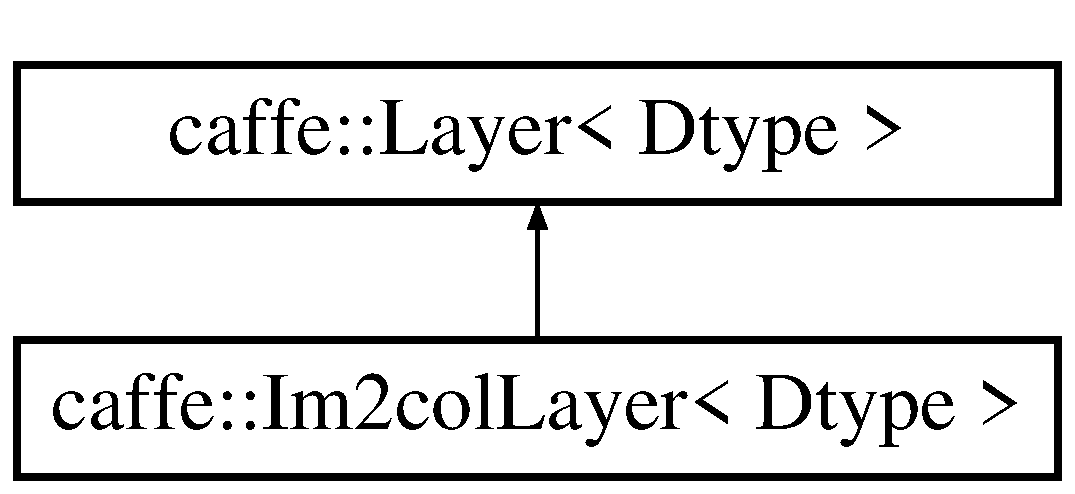
\includegraphics[height=2.000000cm]{classcaffe_1_1Im2colLayer}
\end{center}
\end{figure}
\subsection*{Public Member Functions}
\begin{DoxyCompactItemize}
\item 
{\bfseries Im2col\+Layer} (const Layer\+Parameter \&param)\hypertarget{classcaffe_1_1Im2colLayer_aec089ca3ca3caf3d32193b9dcb2f98e1}{}\label{classcaffe_1_1Im2colLayer_aec089ca3ca3caf3d32193b9dcb2f98e1}

\item 
virtual void \hyperlink{classcaffe_1_1Im2colLayer_a73d7e780b38406dc3d840649cadf8f8a}{Layer\+Set\+Up} (const vector$<$ \hyperlink{classcaffe_1_1Blob}{Blob}$<$ Dtype $>$ $\ast$ $>$ \&bottom, const vector$<$ \hyperlink{classcaffe_1_1Blob}{Blob}$<$ Dtype $>$ $\ast$ $>$ \&top)
\begin{DoxyCompactList}\small\item\em Does layer-\/specific setup\+: your layer should implement this function as well as Reshape. \end{DoxyCompactList}\item 
virtual void \hyperlink{classcaffe_1_1Im2colLayer_a79735ab9fb43a53e4ca02e33a0b3f181}{Reshape} (const vector$<$ \hyperlink{classcaffe_1_1Blob}{Blob}$<$ Dtype $>$ $\ast$ $>$ \&bottom, const vector$<$ \hyperlink{classcaffe_1_1Blob}{Blob}$<$ Dtype $>$ $\ast$ $>$ \&top)
\begin{DoxyCompactList}\small\item\em Adjust the shapes of top blobs and internal buffers to accommodate the shapes of the bottom blobs. \end{DoxyCompactList}\item 
virtual const char $\ast$ \hyperlink{classcaffe_1_1Im2colLayer_aac44aaa893e6fb774c1953b523180cea}{type} () const \hypertarget{classcaffe_1_1Im2colLayer_aac44aaa893e6fb774c1953b523180cea}{}\label{classcaffe_1_1Im2colLayer_aac44aaa893e6fb774c1953b523180cea}

\begin{DoxyCompactList}\small\item\em Returns the layer type. \end{DoxyCompactList}\item 
virtual int \hyperlink{classcaffe_1_1Im2colLayer_aba3720be3f1f71f9e44fbfba90ae3ac0}{Exact\+Num\+Bottom\+Blobs} () const 
\begin{DoxyCompactList}\small\item\em Returns the exact number of bottom blobs required by the layer, or -\/1 if no exact number is required. \end{DoxyCompactList}\item 
virtual int \hyperlink{classcaffe_1_1Im2colLayer_aa4aa1cfc956fa1ab3656ad2adf911f32}{Exact\+Num\+Top\+Blobs} () const 
\begin{DoxyCompactList}\small\item\em Returns the exact number of top blobs required by the layer, or -\/1 if no exact number is required. \end{DoxyCompactList}\end{DoxyCompactItemize}
\subsection*{Protected Member Functions}
\begin{DoxyCompactItemize}
\item 
virtual void \hyperlink{classcaffe_1_1Im2colLayer_ad8c319e6628c7c523c2c6a991f9c631a}{Forward\+\_\+cpu} (const vector$<$ \hyperlink{classcaffe_1_1Blob}{Blob}$<$ Dtype $>$ $\ast$ $>$ \&bottom, const vector$<$ \hyperlink{classcaffe_1_1Blob}{Blob}$<$ Dtype $>$ $\ast$ $>$ \&top)\hypertarget{classcaffe_1_1Im2colLayer_ad8c319e6628c7c523c2c6a991f9c631a}{}\label{classcaffe_1_1Im2colLayer_ad8c319e6628c7c523c2c6a991f9c631a}

\begin{DoxyCompactList}\small\item\em Using the C\+PU device, compute the layer output. \end{DoxyCompactList}\item 
virtual void \hyperlink{classcaffe_1_1Im2colLayer_a1481790fce4361eefab8d78bbdd6f0ec}{Forward\+\_\+gpu} (const vector$<$ \hyperlink{classcaffe_1_1Blob}{Blob}$<$ Dtype $>$ $\ast$ $>$ \&bottom, const vector$<$ \hyperlink{classcaffe_1_1Blob}{Blob}$<$ Dtype $>$ $\ast$ $>$ \&top)\hypertarget{classcaffe_1_1Im2colLayer_a1481790fce4361eefab8d78bbdd6f0ec}{}\label{classcaffe_1_1Im2colLayer_a1481790fce4361eefab8d78bbdd6f0ec}

\begin{DoxyCompactList}\small\item\em Using the G\+PU device, compute the layer output. Fall back to \hyperlink{classcaffe_1_1Im2colLayer_ad8c319e6628c7c523c2c6a991f9c631a}{Forward\+\_\+cpu()} if unavailable. \end{DoxyCompactList}\item 
virtual void \hyperlink{classcaffe_1_1Im2colLayer_a3b2dc21acbbe2e174cc83554469c29f5}{Backward\+\_\+cpu} (const vector$<$ \hyperlink{classcaffe_1_1Blob}{Blob}$<$ Dtype $>$ $\ast$ $>$ \&top, const vector$<$ bool $>$ \&propagate\+\_\+down, const vector$<$ \hyperlink{classcaffe_1_1Blob}{Blob}$<$ Dtype $>$ $\ast$ $>$ \&bottom)\hypertarget{classcaffe_1_1Im2colLayer_a3b2dc21acbbe2e174cc83554469c29f5}{}\label{classcaffe_1_1Im2colLayer_a3b2dc21acbbe2e174cc83554469c29f5}

\begin{DoxyCompactList}\small\item\em Using the C\+PU device, compute the gradients for any parameters and for the bottom blobs if propagate\+\_\+down is true. \end{DoxyCompactList}\item 
virtual void \hyperlink{classcaffe_1_1Im2colLayer_a5340f5b2e176beeb6c74428f05e06c7c}{Backward\+\_\+gpu} (const vector$<$ \hyperlink{classcaffe_1_1Blob}{Blob}$<$ Dtype $>$ $\ast$ $>$ \&top, const vector$<$ bool $>$ \&propagate\+\_\+down, const vector$<$ \hyperlink{classcaffe_1_1Blob}{Blob}$<$ Dtype $>$ $\ast$ $>$ \&bottom)\hypertarget{classcaffe_1_1Im2colLayer_a5340f5b2e176beeb6c74428f05e06c7c}{}\label{classcaffe_1_1Im2colLayer_a5340f5b2e176beeb6c74428f05e06c7c}

\begin{DoxyCompactList}\small\item\em Using the G\+PU device, compute the gradients for any parameters and for the bottom blobs if propagate\+\_\+down is true. Fall back to \hyperlink{classcaffe_1_1Im2colLayer_a3b2dc21acbbe2e174cc83554469c29f5}{Backward\+\_\+cpu()} if unavailable. \end{DoxyCompactList}\end{DoxyCompactItemize}
\subsection*{Protected Attributes}
\begin{DoxyCompactItemize}
\item 
\hyperlink{classcaffe_1_1Blob}{Blob}$<$ int $>$ \hyperlink{classcaffe_1_1Im2colLayer_a188e9ea1225c7f373f4d50e2a78dcec7}{kernel\+\_\+shape\+\_\+}\hypertarget{classcaffe_1_1Im2colLayer_a188e9ea1225c7f373f4d50e2a78dcec7}{}\label{classcaffe_1_1Im2colLayer_a188e9ea1225c7f373f4d50e2a78dcec7}

\begin{DoxyCompactList}\small\item\em The spatial dimensions of a filter kernel. \end{DoxyCompactList}\item 
\hyperlink{classcaffe_1_1Blob}{Blob}$<$ int $>$ \hyperlink{classcaffe_1_1Im2colLayer_afb9baa8216b65a8124d4d1d2b719da0f}{stride\+\_\+}\hypertarget{classcaffe_1_1Im2colLayer_afb9baa8216b65a8124d4d1d2b719da0f}{}\label{classcaffe_1_1Im2colLayer_afb9baa8216b65a8124d4d1d2b719da0f}

\begin{DoxyCompactList}\small\item\em The spatial dimensions of the stride. \end{DoxyCompactList}\item 
\hyperlink{classcaffe_1_1Blob}{Blob}$<$ int $>$ \hyperlink{classcaffe_1_1Im2colLayer_a55c335fac2a25ba438a8bf94497c53ec}{pad\+\_\+}\hypertarget{classcaffe_1_1Im2colLayer_a55c335fac2a25ba438a8bf94497c53ec}{}\label{classcaffe_1_1Im2colLayer_a55c335fac2a25ba438a8bf94497c53ec}

\begin{DoxyCompactList}\small\item\em The spatial dimensions of the padding. \end{DoxyCompactList}\item 
\hyperlink{classcaffe_1_1Blob}{Blob}$<$ int $>$ \hyperlink{classcaffe_1_1Im2colLayer_a3420f6068a4befb3b0ed1ffe5ff0e84c}{dilation\+\_\+}\hypertarget{classcaffe_1_1Im2colLayer_a3420f6068a4befb3b0ed1ffe5ff0e84c}{}\label{classcaffe_1_1Im2colLayer_a3420f6068a4befb3b0ed1ffe5ff0e84c}

\begin{DoxyCompactList}\small\item\em The spatial dimensions of the dilation. \end{DoxyCompactList}\item 
int {\bfseries num\+\_\+spatial\+\_\+axes\+\_\+}\hypertarget{classcaffe_1_1Im2colLayer_a09396822f93f78b400e6e0022cbd0b04}{}\label{classcaffe_1_1Im2colLayer_a09396822f93f78b400e6e0022cbd0b04}

\item 
int {\bfseries bottom\+\_\+dim\+\_\+}\hypertarget{classcaffe_1_1Im2colLayer_a3fc7e611b3a47b656158a4b3bce256e7}{}\label{classcaffe_1_1Im2colLayer_a3fc7e611b3a47b656158a4b3bce256e7}

\item 
int {\bfseries top\+\_\+dim\+\_\+}\hypertarget{classcaffe_1_1Im2colLayer_af0ea2d0f8f54ef280e8d1af46926c35b}{}\label{classcaffe_1_1Im2colLayer_af0ea2d0f8f54ef280e8d1af46926c35b}

\item 
int {\bfseries channel\+\_\+axis\+\_\+}\hypertarget{classcaffe_1_1Im2colLayer_ab7775033a0345f84c2f7a7b936b8973e}{}\label{classcaffe_1_1Im2colLayer_ab7775033a0345f84c2f7a7b936b8973e}

\item 
int {\bfseries num\+\_\+}\hypertarget{classcaffe_1_1Im2colLayer_a0d8977015b84d19c6b1c1a4f2af553c3}{}\label{classcaffe_1_1Im2colLayer_a0d8977015b84d19c6b1c1a4f2af553c3}

\item 
int {\bfseries channels\+\_\+}\hypertarget{classcaffe_1_1Im2colLayer_a819581a35ffba22f5df2c0340210c2e9}{}\label{classcaffe_1_1Im2colLayer_a819581a35ffba22f5df2c0340210c2e9}

\item 
bool {\bfseries force\+\_\+nd\+\_\+im2col\+\_\+}\hypertarget{classcaffe_1_1Im2colLayer_a49819777152d22c57105bdb61df009a3}{}\label{classcaffe_1_1Im2colLayer_a49819777152d22c57105bdb61df009a3}

\end{DoxyCompactItemize}


\subsection{Detailed Description}
\subsubsection*{template$<$typename Dtype$>$\\*
class caffe\+::\+Im2col\+Layer$<$ Dtype $>$}

A helper for image operations that rearranges image regions into column vectors. Used by \hyperlink{classcaffe_1_1ConvolutionLayer}{Convolution\+Layer} to perform convolution by matrix multiplication. 

T\+O\+D\+O(dox)\+: thorough documentation for Forward, Backward, and proto params. 

\subsection{Member Function Documentation}
\index{caffe\+::\+Im2col\+Layer@{caffe\+::\+Im2col\+Layer}!Exact\+Num\+Bottom\+Blobs@{Exact\+Num\+Bottom\+Blobs}}
\index{Exact\+Num\+Bottom\+Blobs@{Exact\+Num\+Bottom\+Blobs}!caffe\+::\+Im2col\+Layer@{caffe\+::\+Im2col\+Layer}}
\subsubsection[{\texorpdfstring{Exact\+Num\+Bottom\+Blobs() const }{ExactNumBottomBlobs() const }}]{\setlength{\rightskip}{0pt plus 5cm}template$<$typename Dtype $>$ virtual int {\bf caffe\+::\+Im2col\+Layer}$<$ Dtype $>$\+::Exact\+Num\+Bottom\+Blobs (
\begin{DoxyParamCaption}
{}
\end{DoxyParamCaption}
) const\hspace{0.3cm}{\ttfamily [inline]}, {\ttfamily [virtual]}}\hypertarget{classcaffe_1_1Im2colLayer_aba3720be3f1f71f9e44fbfba90ae3ac0}{}\label{classcaffe_1_1Im2colLayer_aba3720be3f1f71f9e44fbfba90ae3ac0}


Returns the exact number of bottom blobs required by the layer, or -\/1 if no exact number is required. 

This method should be overridden to return a non-\/negative value if your layer expects some exact number of bottom blobs. 

Reimplemented from \hyperlink{classcaffe_1_1Layer_a45c7a7943a8a6735ac433c9be11e0240}{caffe\+::\+Layer$<$ Dtype $>$}.

\index{caffe\+::\+Im2col\+Layer@{caffe\+::\+Im2col\+Layer}!Exact\+Num\+Top\+Blobs@{Exact\+Num\+Top\+Blobs}}
\index{Exact\+Num\+Top\+Blobs@{Exact\+Num\+Top\+Blobs}!caffe\+::\+Im2col\+Layer@{caffe\+::\+Im2col\+Layer}}
\subsubsection[{\texorpdfstring{Exact\+Num\+Top\+Blobs() const }{ExactNumTopBlobs() const }}]{\setlength{\rightskip}{0pt plus 5cm}template$<$typename Dtype $>$ virtual int {\bf caffe\+::\+Im2col\+Layer}$<$ Dtype $>$\+::Exact\+Num\+Top\+Blobs (
\begin{DoxyParamCaption}
{}
\end{DoxyParamCaption}
) const\hspace{0.3cm}{\ttfamily [inline]}, {\ttfamily [virtual]}}\hypertarget{classcaffe_1_1Im2colLayer_aa4aa1cfc956fa1ab3656ad2adf911f32}{}\label{classcaffe_1_1Im2colLayer_aa4aa1cfc956fa1ab3656ad2adf911f32}


Returns the exact number of top blobs required by the layer, or -\/1 if no exact number is required. 

This method should be overridden to return a non-\/negative value if your layer expects some exact number of top blobs. 

Reimplemented from \hyperlink{classcaffe_1_1Layer_aa3c99ed707e8db683a3043412e151af8}{caffe\+::\+Layer$<$ Dtype $>$}.

\index{caffe\+::\+Im2col\+Layer@{caffe\+::\+Im2col\+Layer}!Layer\+Set\+Up@{Layer\+Set\+Up}}
\index{Layer\+Set\+Up@{Layer\+Set\+Up}!caffe\+::\+Im2col\+Layer@{caffe\+::\+Im2col\+Layer}}
\subsubsection[{\texorpdfstring{Layer\+Set\+Up(const vector$<$ Blob$<$ Dtype $>$ $\ast$ $>$ \&bottom, const vector$<$ Blob$<$ Dtype $>$ $\ast$ $>$ \&top)}{LayerSetUp(const vector< Blob< Dtype > * > &bottom, const vector< Blob< Dtype > * > &top)}}]{\setlength{\rightskip}{0pt plus 5cm}template$<$typename Dtype $>$ void {\bf caffe\+::\+Im2col\+Layer}$<$ Dtype $>$\+::Layer\+Set\+Up (
\begin{DoxyParamCaption}
\item[{const vector$<$ {\bf Blob}$<$ Dtype $>$ $\ast$ $>$ \&}]{bottom, }
\item[{const vector$<$ {\bf Blob}$<$ Dtype $>$ $\ast$ $>$ \&}]{top}
\end{DoxyParamCaption}
)\hspace{0.3cm}{\ttfamily [virtual]}}\hypertarget{classcaffe_1_1Im2colLayer_a73d7e780b38406dc3d840649cadf8f8a}{}\label{classcaffe_1_1Im2colLayer_a73d7e780b38406dc3d840649cadf8f8a}


Does layer-\/specific setup\+: your layer should implement this function as well as Reshape. 


\begin{DoxyParams}{Parameters}
{\em bottom} & the preshaped input blobs, whose data fields store the input data for this layer \\
\hline
{\em top} & the allocated but unshaped output blobs\\
\hline
\end{DoxyParams}
This method should do one-\/time layer specific setup. This includes reading and processing relevent parameters from the {\ttfamily layer\+\_\+param\+\_\+}. Setting up the shapes of top blobs and internal buffers should be done in {\ttfamily Reshape}, which will be called before the forward pass to adjust the top blob sizes. 

Reimplemented from \hyperlink{classcaffe_1_1Layer_a38dc2488bf319b8de5a7ac84e0045393}{caffe\+::\+Layer$<$ Dtype $>$}.

\index{caffe\+::\+Im2col\+Layer@{caffe\+::\+Im2col\+Layer}!Reshape@{Reshape}}
\index{Reshape@{Reshape}!caffe\+::\+Im2col\+Layer@{caffe\+::\+Im2col\+Layer}}
\subsubsection[{\texorpdfstring{Reshape(const vector$<$ Blob$<$ Dtype $>$ $\ast$ $>$ \&bottom, const vector$<$ Blob$<$ Dtype $>$ $\ast$ $>$ \&top)}{Reshape(const vector< Blob< Dtype > * > &bottom, const vector< Blob< Dtype > * > &top)}}]{\setlength{\rightskip}{0pt plus 5cm}template$<$typename Dtype $>$ void {\bf caffe\+::\+Im2col\+Layer}$<$ Dtype $>$\+::Reshape (
\begin{DoxyParamCaption}
\item[{const vector$<$ {\bf Blob}$<$ Dtype $>$ $\ast$ $>$ \&}]{bottom, }
\item[{const vector$<$ {\bf Blob}$<$ Dtype $>$ $\ast$ $>$ \&}]{top}
\end{DoxyParamCaption}
)\hspace{0.3cm}{\ttfamily [virtual]}}\hypertarget{classcaffe_1_1Im2colLayer_a79735ab9fb43a53e4ca02e33a0b3f181}{}\label{classcaffe_1_1Im2colLayer_a79735ab9fb43a53e4ca02e33a0b3f181}


Adjust the shapes of top blobs and internal buffers to accommodate the shapes of the bottom blobs. 


\begin{DoxyParams}{Parameters}
{\em bottom} & the input blobs, with the requested input shapes \\
\hline
{\em top} & the top blobs, which should be reshaped as needed\\
\hline
\end{DoxyParams}
This method should reshape top blobs as needed according to the shapes of the bottom (input) blobs, as well as reshaping any internal buffers and making any other necessary adjustments so that the layer can accommodate the bottom blobs. 

Implements \hyperlink{classcaffe_1_1Layer_ad9d391b972c769c0ebee34ca6d1c973e}{caffe\+::\+Layer$<$ Dtype $>$}.



The documentation for this class was generated from the following files\+:\begin{DoxyCompactItemize}
\item 
include/caffe/layers/im2col\+\_\+layer.\+hpp\item 
src/caffe/layers/im2col\+\_\+layer.\+cpp\end{DoxyCompactItemize}

\hypertarget{classcaffe_1_1ImageDataLayer}{}\section{caffe\+:\+:Image\+Data\+Layer$<$ Dtype $>$ Class Template Reference}
\label{classcaffe_1_1ImageDataLayer}\index{caffe\+::\+Image\+Data\+Layer$<$ Dtype $>$@{caffe\+::\+Image\+Data\+Layer$<$ Dtype $>$}}


Provides data to the \hyperlink{classcaffe_1_1Net}{Net} from image files.  




{\ttfamily \#include $<$image\+\_\+data\+\_\+layer.\+hpp$>$}

Inheritance diagram for caffe\+:\+:Image\+Data\+Layer$<$ Dtype $>$\+:\begin{figure}[H]
\begin{center}
\leavevmode
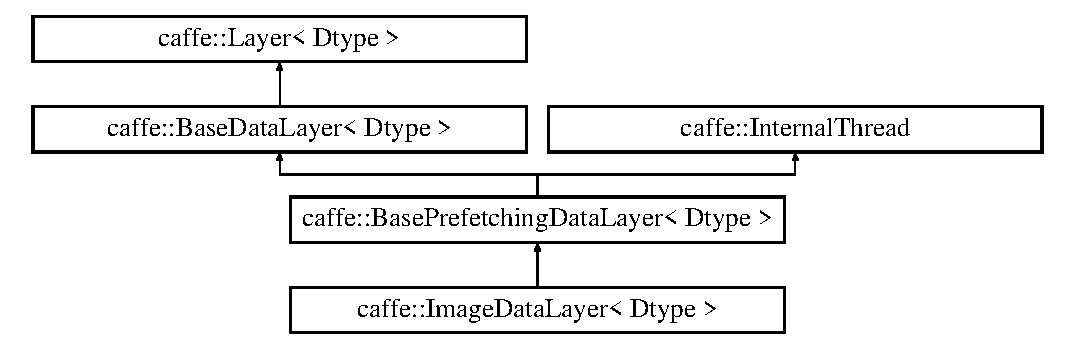
\includegraphics[height=4.000000cm]{classcaffe_1_1ImageDataLayer}
\end{center}
\end{figure}
\subsection*{Public Member Functions}
\begin{DoxyCompactItemize}
\item 
{\bfseries Image\+Data\+Layer} (const Layer\+Parameter \&param)\hypertarget{classcaffe_1_1ImageDataLayer_a2319914181470f8ecd80ffb63d0daec9}{}\label{classcaffe_1_1ImageDataLayer_a2319914181470f8ecd80ffb63d0daec9}

\item 
virtual void {\bfseries Data\+Layer\+Set\+Up} (const vector$<$ \hyperlink{classcaffe_1_1Blob}{Blob}$<$ Dtype $>$ $\ast$ $>$ \&bottom, const vector$<$ \hyperlink{classcaffe_1_1Blob}{Blob}$<$ Dtype $>$ $\ast$ $>$ \&top)\hypertarget{classcaffe_1_1ImageDataLayer_a954e5e3c15c5081569957ded2289cce7}{}\label{classcaffe_1_1ImageDataLayer_a954e5e3c15c5081569957ded2289cce7}

\item 
virtual const char $\ast$ \hyperlink{classcaffe_1_1ImageDataLayer_a5de0c6d7b276d1c540ef7288741a7530}{type} () const \hypertarget{classcaffe_1_1ImageDataLayer_a5de0c6d7b276d1c540ef7288741a7530}{}\label{classcaffe_1_1ImageDataLayer_a5de0c6d7b276d1c540ef7288741a7530}

\begin{DoxyCompactList}\small\item\em Returns the layer type. \end{DoxyCompactList}\item 
virtual int \hyperlink{classcaffe_1_1ImageDataLayer_a95155f868560cf481138deb7a999ee08}{Exact\+Num\+Bottom\+Blobs} () const 
\begin{DoxyCompactList}\small\item\em Returns the exact number of bottom blobs required by the layer, or -\/1 if no exact number is required. \end{DoxyCompactList}\item 
virtual int \hyperlink{classcaffe_1_1ImageDataLayer_a288e0fe3bca4334100e077bc0ad20c60}{Exact\+Num\+Top\+Blobs} () const 
\begin{DoxyCompactList}\small\item\em Returns the exact number of top blobs required by the layer, or -\/1 if no exact number is required. \end{DoxyCompactList}\end{DoxyCompactItemize}
\subsection*{Protected Member Functions}
\begin{DoxyCompactItemize}
\item 
virtual void {\bfseries Shuffle\+Images} ()\hypertarget{classcaffe_1_1ImageDataLayer_a1726e1385072928d37d960c52f0d20b4}{}\label{classcaffe_1_1ImageDataLayer_a1726e1385072928d37d960c52f0d20b4}

\item 
virtual void {\bfseries load\+\_\+batch} (\hyperlink{classcaffe_1_1Batch}{Batch}$<$ Dtype $>$ $\ast$batch)\hypertarget{classcaffe_1_1ImageDataLayer_ae75501864cc0d1e18d8d05b1f601fc89}{}\label{classcaffe_1_1ImageDataLayer_ae75501864cc0d1e18d8d05b1f601fc89}

\end{DoxyCompactItemize}
\subsection*{Protected Attributes}
\begin{DoxyCompactItemize}
\item 
shared\+\_\+ptr$<$ \hyperlink{classcaffe_1_1Caffe_1_1RNG}{Caffe\+::\+R\+NG} $>$ {\bfseries prefetch\+\_\+rng\+\_\+}\hypertarget{classcaffe_1_1ImageDataLayer_a57a7df530e562fa080923aab6c331ab9}{}\label{classcaffe_1_1ImageDataLayer_a57a7df530e562fa080923aab6c331ab9}

\item 
vector$<$ std\+::pair$<$ std\+::string, int $>$ $>$ {\bfseries lines\+\_\+}\hypertarget{classcaffe_1_1ImageDataLayer_a72002dc4459f0d7d739779d734a7c684}{}\label{classcaffe_1_1ImageDataLayer_a72002dc4459f0d7d739779d734a7c684}

\item 
int {\bfseries lines\+\_\+id\+\_\+}\hypertarget{classcaffe_1_1ImageDataLayer_a943f32fdd8d0d37883500b6d83d4243f}{}\label{classcaffe_1_1ImageDataLayer_a943f32fdd8d0d37883500b6d83d4243f}

\end{DoxyCompactItemize}


\subsection{Detailed Description}
\subsubsection*{template$<$typename Dtype$>$\\*
class caffe\+::\+Image\+Data\+Layer$<$ Dtype $>$}

Provides data to the \hyperlink{classcaffe_1_1Net}{Net} from image files. 

T\+O\+D\+O(dox)\+: thorough documentation for Forward and proto params. 

\subsection{Member Function Documentation}
\index{caffe\+::\+Image\+Data\+Layer@{caffe\+::\+Image\+Data\+Layer}!Exact\+Num\+Bottom\+Blobs@{Exact\+Num\+Bottom\+Blobs}}
\index{Exact\+Num\+Bottom\+Blobs@{Exact\+Num\+Bottom\+Blobs}!caffe\+::\+Image\+Data\+Layer@{caffe\+::\+Image\+Data\+Layer}}
\subsubsection[{\texorpdfstring{Exact\+Num\+Bottom\+Blobs() const }{ExactNumBottomBlobs() const }}]{\setlength{\rightskip}{0pt plus 5cm}template$<$typename Dtype $>$ virtual int {\bf caffe\+::\+Image\+Data\+Layer}$<$ Dtype $>$\+::Exact\+Num\+Bottom\+Blobs (
\begin{DoxyParamCaption}
{}
\end{DoxyParamCaption}
) const\hspace{0.3cm}{\ttfamily [inline]}, {\ttfamily [virtual]}}\hypertarget{classcaffe_1_1ImageDataLayer_a95155f868560cf481138deb7a999ee08}{}\label{classcaffe_1_1ImageDataLayer_a95155f868560cf481138deb7a999ee08}


Returns the exact number of bottom blobs required by the layer, or -\/1 if no exact number is required. 

This method should be overridden to return a non-\/negative value if your layer expects some exact number of bottom blobs. 

Reimplemented from \hyperlink{classcaffe_1_1Layer_a45c7a7943a8a6735ac433c9be11e0240}{caffe\+::\+Layer$<$ Dtype $>$}.

\index{caffe\+::\+Image\+Data\+Layer@{caffe\+::\+Image\+Data\+Layer}!Exact\+Num\+Top\+Blobs@{Exact\+Num\+Top\+Blobs}}
\index{Exact\+Num\+Top\+Blobs@{Exact\+Num\+Top\+Blobs}!caffe\+::\+Image\+Data\+Layer@{caffe\+::\+Image\+Data\+Layer}}
\subsubsection[{\texorpdfstring{Exact\+Num\+Top\+Blobs() const }{ExactNumTopBlobs() const }}]{\setlength{\rightskip}{0pt plus 5cm}template$<$typename Dtype $>$ virtual int {\bf caffe\+::\+Image\+Data\+Layer}$<$ Dtype $>$\+::Exact\+Num\+Top\+Blobs (
\begin{DoxyParamCaption}
{}
\end{DoxyParamCaption}
) const\hspace{0.3cm}{\ttfamily [inline]}, {\ttfamily [virtual]}}\hypertarget{classcaffe_1_1ImageDataLayer_a288e0fe3bca4334100e077bc0ad20c60}{}\label{classcaffe_1_1ImageDataLayer_a288e0fe3bca4334100e077bc0ad20c60}


Returns the exact number of top blobs required by the layer, or -\/1 if no exact number is required. 

This method should be overridden to return a non-\/negative value if your layer expects some exact number of top blobs. 

Reimplemented from \hyperlink{classcaffe_1_1Layer_aa3c99ed707e8db683a3043412e151af8}{caffe\+::\+Layer$<$ Dtype $>$}.



The documentation for this class was generated from the following file\+:\begin{DoxyCompactItemize}
\item 
include/caffe/layers/image\+\_\+data\+\_\+layer.\+hpp\end{DoxyCompactItemize}

\hypertarget{classcaffe_1_1InfogainLossLayer}{}\section{caffe\+:\+:Infogain\+Loss\+Layer$<$ Dtype $>$ Class Template Reference}
\label{classcaffe_1_1InfogainLossLayer}\index{caffe\+::\+Infogain\+Loss\+Layer$<$ Dtype $>$@{caffe\+::\+Infogain\+Loss\+Layer$<$ Dtype $>$}}


A generalization of \hyperlink{classcaffe_1_1SoftmaxWithLossLayer}{Softmax\+With\+Loss\+Layer} that takes an \char`\"{}information gain\char`\"{} (infogain) matrix specifying the \char`\"{}value\char`\"{} of all label pairs.  




{\ttfamily \#include $<$infogain\+\_\+loss\+\_\+layer.\+hpp$>$}

Inheritance diagram for caffe\+:\+:Infogain\+Loss\+Layer$<$ Dtype $>$\+:\begin{figure}[H]
\begin{center}
\leavevmode
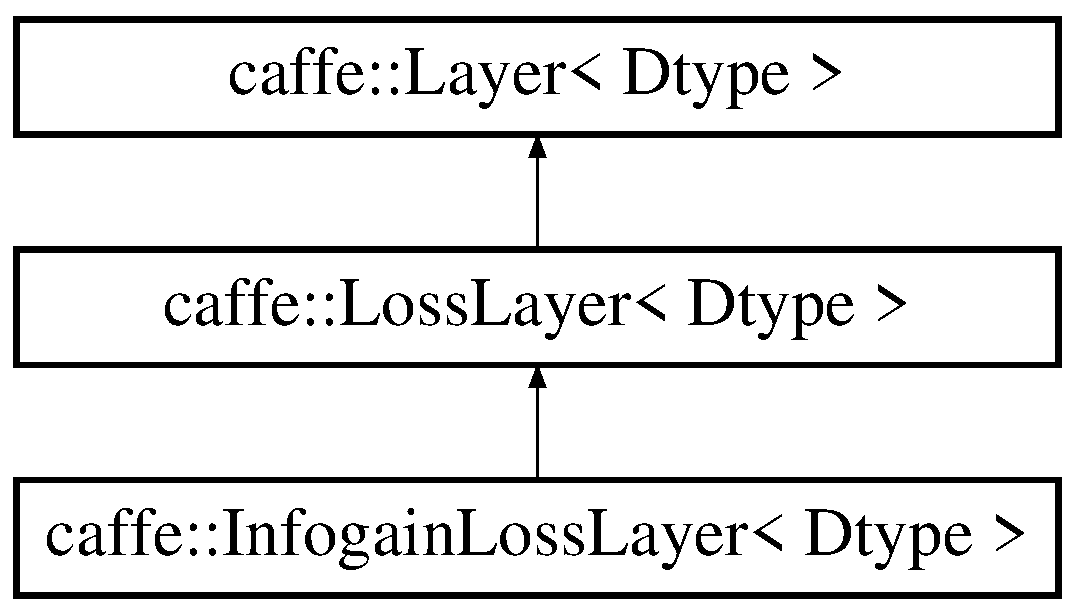
\includegraphics[height=3.000000cm]{classcaffe_1_1InfogainLossLayer}
\end{center}
\end{figure}
\subsection*{Public Member Functions}
\begin{DoxyCompactItemize}
\item 
{\bfseries Infogain\+Loss\+Layer} (const Layer\+Parameter \&param)\hypertarget{classcaffe_1_1InfogainLossLayer_ac2269ba8dc7d18fa8fab90ea9f295784}{}\label{classcaffe_1_1InfogainLossLayer_ac2269ba8dc7d18fa8fab90ea9f295784}

\item 
virtual void \hyperlink{classcaffe_1_1InfogainLossLayer_a55a1d7ae2db81750c33ef9286764cd29}{Layer\+Set\+Up} (const vector$<$ \hyperlink{classcaffe_1_1Blob}{Blob}$<$ Dtype $>$ $\ast$ $>$ \&bottom, const vector$<$ \hyperlink{classcaffe_1_1Blob}{Blob}$<$ Dtype $>$ $\ast$ $>$ \&top)
\begin{DoxyCompactList}\small\item\em Does layer-\/specific setup\+: your layer should implement this function as well as Reshape. \end{DoxyCompactList}\item 
virtual void \hyperlink{classcaffe_1_1InfogainLossLayer_aa1c32ab8252309cb51ed44cacf88f119}{Reshape} (const vector$<$ \hyperlink{classcaffe_1_1Blob}{Blob}$<$ Dtype $>$ $\ast$ $>$ \&bottom, const vector$<$ \hyperlink{classcaffe_1_1Blob}{Blob}$<$ Dtype $>$ $\ast$ $>$ \&top)
\begin{DoxyCompactList}\small\item\em Adjust the shapes of top blobs and internal buffers to accommodate the shapes of the bottom blobs. \end{DoxyCompactList}\item 
virtual int \hyperlink{classcaffe_1_1InfogainLossLayer_aef9aa9200a3129d7bddf56f717017cbb}{Exact\+Num\+Bottom\+Blobs} () const 
\begin{DoxyCompactList}\small\item\em Returns the exact number of bottom blobs required by the layer, or -\/1 if no exact number is required. \end{DoxyCompactList}\item 
virtual int \hyperlink{classcaffe_1_1InfogainLossLayer_a71105feb6b206d7f807c86d7dc303c64}{Min\+Bottom\+Blobs} () const 
\begin{DoxyCompactList}\small\item\em Returns the minimum number of bottom blobs required by the layer, or -\/1 if no minimum number is required. \end{DoxyCompactList}\item 
virtual int \hyperlink{classcaffe_1_1InfogainLossLayer_ae6cf4ae009630b28583b161c33b582cb}{Max\+Bottom\+Blobs} () const 
\begin{DoxyCompactList}\small\item\em Returns the maximum number of bottom blobs required by the layer, or -\/1 if no maximum number is required. \end{DoxyCompactList}\item 
virtual int \hyperlink{classcaffe_1_1InfogainLossLayer_aa25f7b12805d10dccc217669f589fc95}{Exact\+Num\+Top\+Blobs} () const 
\begin{DoxyCompactList}\small\item\em Returns the exact number of top blobs required by the layer, or -\/1 if no exact number is required. \end{DoxyCompactList}\item 
virtual int \hyperlink{classcaffe_1_1InfogainLossLayer_ab7281f377aae57aa744a6b83bed02111}{Min\+Top\+Blobs} () const 
\begin{DoxyCompactList}\small\item\em Returns the minimum number of top blobs required by the layer, or -\/1 if no minimum number is required. \end{DoxyCompactList}\item 
virtual int \hyperlink{classcaffe_1_1InfogainLossLayer_ab77d568acf51c32b8a28bfc45504d382}{Max\+Top\+Blobs} () const 
\begin{DoxyCompactList}\small\item\em Returns the maximum number of top blobs required by the layer, or -\/1 if no maximum number is required. \end{DoxyCompactList}\item 
virtual const char $\ast$ \hyperlink{classcaffe_1_1InfogainLossLayer_ab8056925c12f917270f60d843f840d63}{type} () const \hypertarget{classcaffe_1_1InfogainLossLayer_ab8056925c12f917270f60d843f840d63}{}\label{classcaffe_1_1InfogainLossLayer_ab8056925c12f917270f60d843f840d63}

\begin{DoxyCompactList}\small\item\em Returns the layer type. \end{DoxyCompactList}\end{DoxyCompactItemize}
\subsection*{Protected Member Functions}
\begin{DoxyCompactItemize}
\item 
virtual void \hyperlink{classcaffe_1_1InfogainLossLayer_a33234c8a1d0182dbb20ca3d69687bf65}{Forward\+\_\+cpu} (const vector$<$ \hyperlink{classcaffe_1_1Blob}{Blob}$<$ Dtype $>$ $\ast$ $>$ \&bottom, const vector$<$ \hyperlink{classcaffe_1_1Blob}{Blob}$<$ Dtype $>$ $\ast$ $>$ \&top)
\begin{DoxyCompactList}\small\item\em A generalization of \hyperlink{classcaffe_1_1SoftmaxWithLossLayer}{Softmax\+With\+Loss\+Layer} that takes an \char`\"{}information gain\char`\"{} (infogain) matrix specifying the \char`\"{}value\char`\"{} of all label pairs. \end{DoxyCompactList}\item 
virtual void \hyperlink{classcaffe_1_1InfogainLossLayer_aa17e25c5b0a4a485b5c09456136c9415}{Backward\+\_\+cpu} (const vector$<$ \hyperlink{classcaffe_1_1Blob}{Blob}$<$ Dtype $>$ $\ast$ $>$ \&top, const vector$<$ bool $>$ \&propagate\+\_\+down, const vector$<$ \hyperlink{classcaffe_1_1Blob}{Blob}$<$ Dtype $>$ $\ast$ $>$ \&bottom)
\begin{DoxyCompactList}\small\item\em Computes the infogain loss error gradient w.\+r.\+t. the predictions. \end{DoxyCompactList}\item 
virtual Dtype \hyperlink{classcaffe_1_1InfogainLossLayer_a0e5e9667b19fb88ece7298e3e83d2fdb}{get\+\_\+normalizer} (Loss\+Parameter\+\_\+\+Normalization\+Mode normalization\+\_\+mode, int valid\+\_\+count)
\item 
virtual void \hyperlink{classcaffe_1_1InfogainLossLayer_a030296e6af30acd17a3cfe4463456147}{sum\+\_\+rows\+\_\+of\+\_\+H} (const \hyperlink{classcaffe_1_1Blob}{Blob}$<$ Dtype $>$ $\ast$H)\hypertarget{classcaffe_1_1InfogainLossLayer_a030296e6af30acd17a3cfe4463456147}{}\label{classcaffe_1_1InfogainLossLayer_a030296e6af30acd17a3cfe4463456147}

\begin{DoxyCompactList}\small\item\em fill sum\+\_\+rows\+\_\+\+H\+\_\+ according to matrix H \end{DoxyCompactList}\end{DoxyCompactItemize}
\subsection*{Protected Attributes}
\begin{DoxyCompactItemize}
\item 
shared\+\_\+ptr$<$ \hyperlink{classcaffe_1_1Layer}{Layer}$<$ Dtype $>$ $>$ \hyperlink{classcaffe_1_1InfogainLossLayer_a1992ffcac64ab6d61ebce80c7d9e8405}{softmax\+\_\+layer\+\_\+}\hypertarget{classcaffe_1_1InfogainLossLayer_a1992ffcac64ab6d61ebce80c7d9e8405}{}\label{classcaffe_1_1InfogainLossLayer_a1992ffcac64ab6d61ebce80c7d9e8405}

\begin{DoxyCompactList}\small\item\em The internal \hyperlink{classcaffe_1_1SoftmaxLayer}{Softmax\+Layer} used to map predictions to a distribution. \end{DoxyCompactList}\item 
\hyperlink{classcaffe_1_1Blob}{Blob}$<$ Dtype $>$ \hyperlink{classcaffe_1_1InfogainLossLayer_a4ae881c2950ca84a50b0f964797defd6}{prob\+\_\+}\hypertarget{classcaffe_1_1InfogainLossLayer_a4ae881c2950ca84a50b0f964797defd6}{}\label{classcaffe_1_1InfogainLossLayer_a4ae881c2950ca84a50b0f964797defd6}

\begin{DoxyCompactList}\small\item\em prob stores the output probability predictions from the \hyperlink{classcaffe_1_1SoftmaxLayer}{Softmax\+Layer}. \end{DoxyCompactList}\item 
vector$<$ \hyperlink{classcaffe_1_1Blob}{Blob}$<$ Dtype $>$ $\ast$ $>$ \hyperlink{classcaffe_1_1InfogainLossLayer_ad919452e3fbb182cf56ded1e32ee001d}{softmax\+\_\+bottom\+\_\+vec\+\_\+}\hypertarget{classcaffe_1_1InfogainLossLayer_ad919452e3fbb182cf56ded1e32ee001d}{}\label{classcaffe_1_1InfogainLossLayer_ad919452e3fbb182cf56ded1e32ee001d}

\begin{DoxyCompactList}\small\item\em bottom vector holder used in call to the underlying \hyperlink{classcaffe_1_1Layer_aa5fc9ddb31b58958653372bdaaccde94}{Softmax\+Layer\+::\+Forward} \end{DoxyCompactList}\item 
vector$<$ \hyperlink{classcaffe_1_1Blob}{Blob}$<$ Dtype $>$ $\ast$ $>$ \hyperlink{classcaffe_1_1InfogainLossLayer_abce0ff34e57ed3660e39633535c97e41}{softmax\+\_\+top\+\_\+vec\+\_\+}\hypertarget{classcaffe_1_1InfogainLossLayer_abce0ff34e57ed3660e39633535c97e41}{}\label{classcaffe_1_1InfogainLossLayer_abce0ff34e57ed3660e39633535c97e41}

\begin{DoxyCompactList}\small\item\em top vector holder used in call to the underlying \hyperlink{classcaffe_1_1Layer_aa5fc9ddb31b58958653372bdaaccde94}{Softmax\+Layer\+::\+Forward} \end{DoxyCompactList}\item 
\hyperlink{classcaffe_1_1Blob}{Blob}$<$ Dtype $>$ {\bfseries infogain\+\_\+}\hypertarget{classcaffe_1_1InfogainLossLayer_a2d9ffe8c64b096042cc75fced30dcaca}{}\label{classcaffe_1_1InfogainLossLayer_a2d9ffe8c64b096042cc75fced30dcaca}

\item 
\hyperlink{classcaffe_1_1Blob}{Blob}$<$ Dtype $>$ {\bfseries sum\+\_\+rows\+\_\+\+H\+\_\+}\hypertarget{classcaffe_1_1InfogainLossLayer_a4f3a277e92ec66b9ad09d3a0fddcd595}{}\label{classcaffe_1_1InfogainLossLayer_a4f3a277e92ec66b9ad09d3a0fddcd595}

\item 
bool \hyperlink{classcaffe_1_1InfogainLossLayer_a421720fc0f85daf8b6b7808719b1f9e8}{has\+\_\+ignore\+\_\+label\+\_\+}\hypertarget{classcaffe_1_1InfogainLossLayer_a421720fc0f85daf8b6b7808719b1f9e8}{}\label{classcaffe_1_1InfogainLossLayer_a421720fc0f85daf8b6b7808719b1f9e8}

\begin{DoxyCompactList}\small\item\em Whether to ignore instances with a certain label. \end{DoxyCompactList}\item 
int \hyperlink{classcaffe_1_1InfogainLossLayer_ad3f7c2efdf32f99510186495ba7c5cff}{ignore\+\_\+label\+\_\+}\hypertarget{classcaffe_1_1InfogainLossLayer_ad3f7c2efdf32f99510186495ba7c5cff}{}\label{classcaffe_1_1InfogainLossLayer_ad3f7c2efdf32f99510186495ba7c5cff}

\begin{DoxyCompactList}\small\item\em The label indicating that an instance should be ignored. \end{DoxyCompactList}\item 
Loss\+Parameter\+\_\+\+Normalization\+Mode \hyperlink{classcaffe_1_1InfogainLossLayer_ab7fe88c996d31d67f5e13fc0ffc803c2}{normalization\+\_\+}\hypertarget{classcaffe_1_1InfogainLossLayer_ab7fe88c996d31d67f5e13fc0ffc803c2}{}\label{classcaffe_1_1InfogainLossLayer_ab7fe88c996d31d67f5e13fc0ffc803c2}

\begin{DoxyCompactList}\small\item\em How to normalize the output loss. \end{DoxyCompactList}\item 
int {\bfseries infogain\+\_\+axis\+\_\+}\hypertarget{classcaffe_1_1InfogainLossLayer_a0f94b595bd8be01b31994236af8cecbd}{}\label{classcaffe_1_1InfogainLossLayer_a0f94b595bd8be01b31994236af8cecbd}

\item 
int {\bfseries outer\+\_\+num\+\_\+}\hypertarget{classcaffe_1_1InfogainLossLayer_aaf878e99cf00ac309ed533adf43bcbc3}{}\label{classcaffe_1_1InfogainLossLayer_aaf878e99cf00ac309ed533adf43bcbc3}

\item 
int {\bfseries inner\+\_\+num\+\_\+}\hypertarget{classcaffe_1_1InfogainLossLayer_a6707b103411c0acc3fddd065e91fe6e0}{}\label{classcaffe_1_1InfogainLossLayer_a6707b103411c0acc3fddd065e91fe6e0}

\item 
int {\bfseries num\+\_\+labels\+\_\+}\hypertarget{classcaffe_1_1InfogainLossLayer_a8b58f39c561263cfa44c3831e6a15355}{}\label{classcaffe_1_1InfogainLossLayer_a8b58f39c561263cfa44c3831e6a15355}

\end{DoxyCompactItemize}


\subsection{Detailed Description}
\subsubsection*{template$<$typename Dtype$>$\\*
class caffe\+::\+Infogain\+Loss\+Layer$<$ Dtype $>$}

A generalization of \hyperlink{classcaffe_1_1SoftmaxWithLossLayer}{Softmax\+With\+Loss\+Layer} that takes an \char`\"{}information gain\char`\"{} (infogain) matrix specifying the \char`\"{}value\char`\"{} of all label pairs. 

Equivalent to the \hyperlink{classcaffe_1_1SoftmaxWithLossLayer}{Softmax\+With\+Loss\+Layer} if the infogain matrix is the identity.


\begin{DoxyParams}{Parameters}
{\em bottom} & input \hyperlink{classcaffe_1_1Blob}{Blob} vector (length 2-\/3)
\begin{DoxyEnumerate}
\item $ (N \times C \times H \times W) $ the predictions $ x $, a \hyperlink{classcaffe_1_1Blob}{Blob} with values in $ [-\infty, +\infty] $ indicating the predicted score for each of the $ K = CHW $ classes. This layer maps these scores to a probability distribution over classes using the softmax function $ \hat{p}_{nk} = \exp(x_{nk}) / \left[\sum_{k'} \exp(x_{nk'})\right] $ (see \hyperlink{classcaffe_1_1SoftmaxLayer}{Softmax\+Layer}).
\item $ (N \times 1 \times 1 \times 1) $ the labels $ l $, an integer-\/valued \hyperlink{classcaffe_1_1Blob}{Blob} with values $ l_n \in [0, 1, 2, ..., K - 1] $ indicating the correct class label among the $ K $ classes
\item $ (1 \times 1 \times K \times K) $ ({\bfseries optional}) the infogain matrix $ H $. This must be provided as the third bottom blob input if not provided as the infogain\+\_\+mat in the Infogain\+Loss\+Parameter. If $ H = I $, this layer is equivalent to the \hyperlink{classcaffe_1_1SoftmaxWithLossLayer}{Softmax\+With\+Loss\+Layer}. 
\end{DoxyEnumerate}\\
\hline
{\em top} & output \hyperlink{classcaffe_1_1Blob}{Blob} vector (length 1)
\begin{DoxyEnumerate}
\item $ (1 \times 1 \times 1 \times 1) $ the computed infogain multinomial logistic loss\+: $ E = \frac{-1}{N} \sum\limits_{n=1}^N H_{l_n} \log(\hat{p}_n) = \frac{-1}{N} \sum\limits_{n=1}^N \sum\limits_{k=1}^{K} H_{l_n,k} \log(\hat{p}_{n,k}) $, where $ H_{l_n} $ denotes row $l_n$ of $H$. 
\end{DoxyEnumerate}\\
\hline
\end{DoxyParams}


\subsection{Member Function Documentation}
\index{caffe\+::\+Infogain\+Loss\+Layer@{caffe\+::\+Infogain\+Loss\+Layer}!Backward\+\_\+cpu@{Backward\+\_\+cpu}}
\index{Backward\+\_\+cpu@{Backward\+\_\+cpu}!caffe\+::\+Infogain\+Loss\+Layer@{caffe\+::\+Infogain\+Loss\+Layer}}
\subsubsection[{\texorpdfstring{Backward\+\_\+cpu(const vector$<$ Blob$<$ Dtype $>$ $\ast$ $>$ \&top, const vector$<$ bool $>$ \&propagate\+\_\+down, const vector$<$ Blob$<$ Dtype $>$ $\ast$ $>$ \&bottom)}{Backward_cpu(const vector< Blob< Dtype > * > &top, const vector< bool > &propagate_down, const vector< Blob< Dtype > * > &bottom)}}]{\setlength{\rightskip}{0pt plus 5cm}template$<$typename Dtype $>$ void {\bf caffe\+::\+Infogain\+Loss\+Layer}$<$ Dtype $>$\+::Backward\+\_\+cpu (
\begin{DoxyParamCaption}
\item[{const vector$<$ {\bf Blob}$<$ Dtype $>$ $\ast$ $>$ \&}]{top, }
\item[{const vector$<$ bool $>$ \&}]{propagate\+\_\+down, }
\item[{const vector$<$ {\bf Blob}$<$ Dtype $>$ $\ast$ $>$ \&}]{bottom}
\end{DoxyParamCaption}
)\hspace{0.3cm}{\ttfamily [protected]}, {\ttfamily [virtual]}}\hypertarget{classcaffe_1_1InfogainLossLayer_aa17e25c5b0a4a485b5c09456136c9415}{}\label{classcaffe_1_1InfogainLossLayer_aa17e25c5b0a4a485b5c09456136c9415}


Computes the infogain loss error gradient w.\+r.\+t. the predictions. 

Gradients cannot be computed with respect to the label inputs (bottom\mbox{[}1\mbox{]}), so this method ignores bottom\mbox{[}1\mbox{]} and requires !propagate\+\_\+down\mbox{[}1\mbox{]}, crashing if propagate\+\_\+down\mbox{[}1\mbox{]} is set. (The same applies to the infogain matrix, if provided as bottom\mbox{[}2\mbox{]} rather than in the layer\+\_\+param.)


\begin{DoxyParams}{Parameters}
{\em top} & output \hyperlink{classcaffe_1_1Blob}{Blob} vector (length 1), providing the error gradient with respect to the outputs
\begin{DoxyEnumerate}
\item $ (1 \times 1 \times 1 \times 1) $ This \hyperlink{classcaffe_1_1Blob}{Blob}\textquotesingle{}s diff will simply contain the loss\+\_\+weight$\ast$ $ \lambda $, as $ \lambda $ is the coefficient of this layer\textquotesingle{}s output $\ell_i$ in the overall \hyperlink{classcaffe_1_1Net}{Net} loss $ E = \lambda_i \ell_i + \mbox{other loss terms}$; hence $ \frac{\partial E}{\partial \ell_i} = \lambda_i $. ($\ast$\+Assuming that this top \hyperlink{classcaffe_1_1Blob}{Blob} is not used as a bottom (input) by any other layer of the \hyperlink{classcaffe_1_1Net}{Net}.) 
\end{DoxyEnumerate}\\
\hline
{\em propagate\+\_\+down} & see \hyperlink{classcaffe_1_1Layer_a53df1e081767e07bfb4c81657f4acd0a}{Layer\+::\+Backward}. propagate\+\_\+down\mbox{[}1\mbox{]} must be false as we can\textquotesingle{}t compute gradients with respect to the labels (similarly for propagate\+\_\+down\mbox{[}2\mbox{]} and the infogain matrix, if provided as bottom\mbox{[}2\mbox{]}) \\
\hline
{\em bottom} & input \hyperlink{classcaffe_1_1Blob}{Blob} vector (length 2-\/3)
\begin{DoxyEnumerate}
\item $ (N \times C \times H \times W) $ the predictions $ x $; Backward computes diff $ \frac{\partial E}{\partial x} $
\item $ (N \times 1 \times 1 \times 1) $ the labels -- ignored as we can\textquotesingle{}t compute their error gradients
\item $ (1 \times 1 \times K \times K) $ ({\bfseries optional}) the information gain matrix -- ignored as its error gradient computation is not implemented. 
\end{DoxyEnumerate}\\
\hline
\end{DoxyParams}


Implements \hyperlink{classcaffe_1_1Layer_a64d15855f882af4b82e83fa993c4e7c6}{caffe\+::\+Layer$<$ Dtype $>$}.

\index{caffe\+::\+Infogain\+Loss\+Layer@{caffe\+::\+Infogain\+Loss\+Layer}!Exact\+Num\+Bottom\+Blobs@{Exact\+Num\+Bottom\+Blobs}}
\index{Exact\+Num\+Bottom\+Blobs@{Exact\+Num\+Bottom\+Blobs}!caffe\+::\+Infogain\+Loss\+Layer@{caffe\+::\+Infogain\+Loss\+Layer}}
\subsubsection[{\texorpdfstring{Exact\+Num\+Bottom\+Blobs() const }{ExactNumBottomBlobs() const }}]{\setlength{\rightskip}{0pt plus 5cm}template$<$typename Dtype $>$ virtual int {\bf caffe\+::\+Infogain\+Loss\+Layer}$<$ Dtype $>$\+::Exact\+Num\+Bottom\+Blobs (
\begin{DoxyParamCaption}
{}
\end{DoxyParamCaption}
) const\hspace{0.3cm}{\ttfamily [inline]}, {\ttfamily [virtual]}}\hypertarget{classcaffe_1_1InfogainLossLayer_aef9aa9200a3129d7bddf56f717017cbb}{}\label{classcaffe_1_1InfogainLossLayer_aef9aa9200a3129d7bddf56f717017cbb}


Returns the exact number of bottom blobs required by the layer, or -\/1 if no exact number is required. 

This method should be overridden to return a non-\/negative value if your layer expects some exact number of bottom blobs. 

Reimplemented from \hyperlink{classcaffe_1_1LossLayer_a8a2e16d4691640c34e589aac4ec42e28}{caffe\+::\+Loss\+Layer$<$ Dtype $>$}.

\index{caffe\+::\+Infogain\+Loss\+Layer@{caffe\+::\+Infogain\+Loss\+Layer}!Exact\+Num\+Top\+Blobs@{Exact\+Num\+Top\+Blobs}}
\index{Exact\+Num\+Top\+Blobs@{Exact\+Num\+Top\+Blobs}!caffe\+::\+Infogain\+Loss\+Layer@{caffe\+::\+Infogain\+Loss\+Layer}}
\subsubsection[{\texorpdfstring{Exact\+Num\+Top\+Blobs() const }{ExactNumTopBlobs() const }}]{\setlength{\rightskip}{0pt plus 5cm}template$<$typename Dtype $>$ virtual int {\bf caffe\+::\+Infogain\+Loss\+Layer}$<$ Dtype $>$\+::Exact\+Num\+Top\+Blobs (
\begin{DoxyParamCaption}
{}
\end{DoxyParamCaption}
) const\hspace{0.3cm}{\ttfamily [inline]}, {\ttfamily [virtual]}}\hypertarget{classcaffe_1_1InfogainLossLayer_aa25f7b12805d10dccc217669f589fc95}{}\label{classcaffe_1_1InfogainLossLayer_aa25f7b12805d10dccc217669f589fc95}


Returns the exact number of top blobs required by the layer, or -\/1 if no exact number is required. 

This method should be overridden to return a non-\/negative value if your layer expects some exact number of top blobs. 

Reimplemented from \hyperlink{classcaffe_1_1LossLayer_af8dca16967e8e979ebead4e80664dc10}{caffe\+::\+Loss\+Layer$<$ Dtype $>$}.

\index{caffe\+::\+Infogain\+Loss\+Layer@{caffe\+::\+Infogain\+Loss\+Layer}!Forward\+\_\+cpu@{Forward\+\_\+cpu}}
\index{Forward\+\_\+cpu@{Forward\+\_\+cpu}!caffe\+::\+Infogain\+Loss\+Layer@{caffe\+::\+Infogain\+Loss\+Layer}}
\subsubsection[{\texorpdfstring{Forward\+\_\+cpu(const vector$<$ Blob$<$ Dtype $>$ $\ast$ $>$ \&bottom, const vector$<$ Blob$<$ Dtype $>$ $\ast$ $>$ \&top)}{Forward_cpu(const vector< Blob< Dtype > * > &bottom, const vector< Blob< Dtype > * > &top)}}]{\setlength{\rightskip}{0pt plus 5cm}template$<$typename Dtype $>$ void {\bf caffe\+::\+Infogain\+Loss\+Layer}$<$ Dtype $>$\+::Forward\+\_\+cpu (
\begin{DoxyParamCaption}
\item[{const vector$<$ {\bf Blob}$<$ Dtype $>$ $\ast$ $>$ \&}]{bottom, }
\item[{const vector$<$ {\bf Blob}$<$ Dtype $>$ $\ast$ $>$ \&}]{top}
\end{DoxyParamCaption}
)\hspace{0.3cm}{\ttfamily [protected]}, {\ttfamily [virtual]}}\hypertarget{classcaffe_1_1InfogainLossLayer_a33234c8a1d0182dbb20ca3d69687bf65}{}\label{classcaffe_1_1InfogainLossLayer_a33234c8a1d0182dbb20ca3d69687bf65}


A generalization of \hyperlink{classcaffe_1_1SoftmaxWithLossLayer}{Softmax\+With\+Loss\+Layer} that takes an \char`\"{}information gain\char`\"{} (infogain) matrix specifying the \char`\"{}value\char`\"{} of all label pairs. 

Equivalent to the \hyperlink{classcaffe_1_1SoftmaxWithLossLayer}{Softmax\+With\+Loss\+Layer} if the infogain matrix is the identity.


\begin{DoxyParams}{Parameters}
{\em bottom} & input \hyperlink{classcaffe_1_1Blob}{Blob} vector (length 2-\/3)
\begin{DoxyEnumerate}
\item $ (N \times C \times H \times W) $ the predictions $ x $, a \hyperlink{classcaffe_1_1Blob}{Blob} with values in $ [-\infty, +\infty] $ indicating the predicted score for each of the $ K = CHW $ classes. This layer maps these scores to a probability distribution over classes using the softmax function $ \hat{p}_{nk} = \exp(x_{nk}) / \left[\sum_{k'} \exp(x_{nk'})\right] $ (see \hyperlink{classcaffe_1_1SoftmaxLayer}{Softmax\+Layer}).
\item $ (N \times 1 \times 1 \times 1) $ the labels $ l $, an integer-\/valued \hyperlink{classcaffe_1_1Blob}{Blob} with values $ l_n \in [0, 1, 2, ..., K - 1] $ indicating the correct class label among the $ K $ classes
\item $ (1 \times 1 \times K \times K) $ ({\bfseries optional}) the infogain matrix $ H $. This must be provided as the third bottom blob input if not provided as the infogain\+\_\+mat in the Infogain\+Loss\+Parameter. If $ H = I $, this layer is equivalent to the \hyperlink{classcaffe_1_1SoftmaxWithLossLayer}{Softmax\+With\+Loss\+Layer}. 
\end{DoxyEnumerate}\\
\hline
{\em top} & output \hyperlink{classcaffe_1_1Blob}{Blob} vector (length 1)
\begin{DoxyEnumerate}
\item $ (1 \times 1 \times 1 \times 1) $ the computed infogain multinomial logistic loss\+: $ E = \frac{-1}{N} \sum\limits_{n=1}^N H_{l_n} \log(\hat{p}_n) = \frac{-1}{N} \sum\limits_{n=1}^N \sum\limits_{k=1}^{K} H_{l_n,k} \log(\hat{p}_{n,k}) $, where $ H_{l_n} $ denotes row $l_n$ of $H$. 
\end{DoxyEnumerate}\\
\hline
\end{DoxyParams}


Implements \hyperlink{classcaffe_1_1Layer_add965883f75bbf90c7a06f960cda7a1a}{caffe\+::\+Layer$<$ Dtype $>$}.

\index{caffe\+::\+Infogain\+Loss\+Layer@{caffe\+::\+Infogain\+Loss\+Layer}!get\+\_\+normalizer@{get\+\_\+normalizer}}
\index{get\+\_\+normalizer@{get\+\_\+normalizer}!caffe\+::\+Infogain\+Loss\+Layer@{caffe\+::\+Infogain\+Loss\+Layer}}
\subsubsection[{\texorpdfstring{get\+\_\+normalizer(\+Loss\+Parameter\+\_\+\+Normalization\+Mode normalization\+\_\+mode, int valid\+\_\+count)}{get_normalizer(LossParameter_NormalizationMode normalization_mode, int valid_count)}}]{\setlength{\rightskip}{0pt plus 5cm}template$<$typename Dtype $>$ Dtype {\bf caffe\+::\+Infogain\+Loss\+Layer}$<$ Dtype $>$\+::get\+\_\+normalizer (
\begin{DoxyParamCaption}
\item[{Loss\+Parameter\+\_\+\+Normalization\+Mode}]{normalization\+\_\+mode, }
\item[{int}]{valid\+\_\+count}
\end{DoxyParamCaption}
)\hspace{0.3cm}{\ttfamily [protected]}, {\ttfamily [virtual]}}\hypertarget{classcaffe_1_1InfogainLossLayer_a0e5e9667b19fb88ece7298e3e83d2fdb}{}\label{classcaffe_1_1InfogainLossLayer_a0e5e9667b19fb88ece7298e3e83d2fdb}
Read the normalization mode parameter and compute the normalizer based on the blob size. If normalization\+\_\+mode is V\+A\+L\+ID, the count of valid outputs will be read from valid\+\_\+count, unless it is -\/1 in which case all outputs are assumed to be valid. \index{caffe\+::\+Infogain\+Loss\+Layer@{caffe\+::\+Infogain\+Loss\+Layer}!Layer\+Set\+Up@{Layer\+Set\+Up}}
\index{Layer\+Set\+Up@{Layer\+Set\+Up}!caffe\+::\+Infogain\+Loss\+Layer@{caffe\+::\+Infogain\+Loss\+Layer}}
\subsubsection[{\texorpdfstring{Layer\+Set\+Up(const vector$<$ Blob$<$ Dtype $>$ $\ast$ $>$ \&bottom, const vector$<$ Blob$<$ Dtype $>$ $\ast$ $>$ \&top)}{LayerSetUp(const vector< Blob< Dtype > * > &bottom, const vector< Blob< Dtype > * > &top)}}]{\setlength{\rightskip}{0pt plus 5cm}template$<$typename Dtype $>$ void {\bf caffe\+::\+Infogain\+Loss\+Layer}$<$ Dtype $>$\+::Layer\+Set\+Up (
\begin{DoxyParamCaption}
\item[{const vector$<$ {\bf Blob}$<$ Dtype $>$ $\ast$ $>$ \&}]{bottom, }
\item[{const vector$<$ {\bf Blob}$<$ Dtype $>$ $\ast$ $>$ \&}]{top}
\end{DoxyParamCaption}
)\hspace{0.3cm}{\ttfamily [virtual]}}\hypertarget{classcaffe_1_1InfogainLossLayer_a55a1d7ae2db81750c33ef9286764cd29}{}\label{classcaffe_1_1InfogainLossLayer_a55a1d7ae2db81750c33ef9286764cd29}


Does layer-\/specific setup\+: your layer should implement this function as well as Reshape. 


\begin{DoxyParams}{Parameters}
{\em bottom} & the preshaped input blobs, whose data fields store the input data for this layer \\
\hline
{\em top} & the allocated but unshaped output blobs\\
\hline
\end{DoxyParams}
This method should do one-\/time layer specific setup. This includes reading and processing relevent parameters from the {\ttfamily layer\+\_\+param\+\_\+}. Setting up the shapes of top blobs and internal buffers should be done in {\ttfamily Reshape}, which will be called before the forward pass to adjust the top blob sizes. 

Reimplemented from \hyperlink{classcaffe_1_1LossLayer_a98084e06f7ca0e44c11aee5544379609}{caffe\+::\+Loss\+Layer$<$ Dtype $>$}.

\index{caffe\+::\+Infogain\+Loss\+Layer@{caffe\+::\+Infogain\+Loss\+Layer}!Max\+Bottom\+Blobs@{Max\+Bottom\+Blobs}}
\index{Max\+Bottom\+Blobs@{Max\+Bottom\+Blobs}!caffe\+::\+Infogain\+Loss\+Layer@{caffe\+::\+Infogain\+Loss\+Layer}}
\subsubsection[{\texorpdfstring{Max\+Bottom\+Blobs() const }{MaxBottomBlobs() const }}]{\setlength{\rightskip}{0pt plus 5cm}template$<$typename Dtype $>$ virtual int {\bf caffe\+::\+Infogain\+Loss\+Layer}$<$ Dtype $>$\+::Max\+Bottom\+Blobs (
\begin{DoxyParamCaption}
{}
\end{DoxyParamCaption}
) const\hspace{0.3cm}{\ttfamily [inline]}, {\ttfamily [virtual]}}\hypertarget{classcaffe_1_1InfogainLossLayer_ae6cf4ae009630b28583b161c33b582cb}{}\label{classcaffe_1_1InfogainLossLayer_ae6cf4ae009630b28583b161c33b582cb}


Returns the maximum number of bottom blobs required by the layer, or -\/1 if no maximum number is required. 

This method should be overridden to return a non-\/negative value if your layer expects some maximum number of bottom blobs. 

Reimplemented from \hyperlink{classcaffe_1_1Layer_a6408ef3939f1abed1abcec46ff219289}{caffe\+::\+Layer$<$ Dtype $>$}.

\index{caffe\+::\+Infogain\+Loss\+Layer@{caffe\+::\+Infogain\+Loss\+Layer}!Max\+Top\+Blobs@{Max\+Top\+Blobs}}
\index{Max\+Top\+Blobs@{Max\+Top\+Blobs}!caffe\+::\+Infogain\+Loss\+Layer@{caffe\+::\+Infogain\+Loss\+Layer}}
\subsubsection[{\texorpdfstring{Max\+Top\+Blobs() const }{MaxTopBlobs() const }}]{\setlength{\rightskip}{0pt plus 5cm}template$<$typename Dtype $>$ virtual int {\bf caffe\+::\+Infogain\+Loss\+Layer}$<$ Dtype $>$\+::Max\+Top\+Blobs (
\begin{DoxyParamCaption}
{}
\end{DoxyParamCaption}
) const\hspace{0.3cm}{\ttfamily [inline]}, {\ttfamily [virtual]}}\hypertarget{classcaffe_1_1InfogainLossLayer_ab77d568acf51c32b8a28bfc45504d382}{}\label{classcaffe_1_1InfogainLossLayer_ab77d568acf51c32b8a28bfc45504d382}


Returns the maximum number of top blobs required by the layer, or -\/1 if no maximum number is required. 

This method should be overridden to return a non-\/negative value if your layer expects some maximum number of top blobs. 

Reimplemented from \hyperlink{classcaffe_1_1Layer_adeff774663c6ec94424901d2746e2f03}{caffe\+::\+Layer$<$ Dtype $>$}.

\index{caffe\+::\+Infogain\+Loss\+Layer@{caffe\+::\+Infogain\+Loss\+Layer}!Min\+Bottom\+Blobs@{Min\+Bottom\+Blobs}}
\index{Min\+Bottom\+Blobs@{Min\+Bottom\+Blobs}!caffe\+::\+Infogain\+Loss\+Layer@{caffe\+::\+Infogain\+Loss\+Layer}}
\subsubsection[{\texorpdfstring{Min\+Bottom\+Blobs() const }{MinBottomBlobs() const }}]{\setlength{\rightskip}{0pt plus 5cm}template$<$typename Dtype $>$ virtual int {\bf caffe\+::\+Infogain\+Loss\+Layer}$<$ Dtype $>$\+::Min\+Bottom\+Blobs (
\begin{DoxyParamCaption}
{}
\end{DoxyParamCaption}
) const\hspace{0.3cm}{\ttfamily [inline]}, {\ttfamily [virtual]}}\hypertarget{classcaffe_1_1InfogainLossLayer_a71105feb6b206d7f807c86d7dc303c64}{}\label{classcaffe_1_1InfogainLossLayer_a71105feb6b206d7f807c86d7dc303c64}


Returns the minimum number of bottom blobs required by the layer, or -\/1 if no minimum number is required. 

This method should be overridden to return a non-\/negative value if your layer expects some minimum number of bottom blobs. 

Reimplemented from \hyperlink{classcaffe_1_1Layer_ade3eee97cc743c4e68fff7eba6484916}{caffe\+::\+Layer$<$ Dtype $>$}.

\index{caffe\+::\+Infogain\+Loss\+Layer@{caffe\+::\+Infogain\+Loss\+Layer}!Min\+Top\+Blobs@{Min\+Top\+Blobs}}
\index{Min\+Top\+Blobs@{Min\+Top\+Blobs}!caffe\+::\+Infogain\+Loss\+Layer@{caffe\+::\+Infogain\+Loss\+Layer}}
\subsubsection[{\texorpdfstring{Min\+Top\+Blobs() const }{MinTopBlobs() const }}]{\setlength{\rightskip}{0pt plus 5cm}template$<$typename Dtype $>$ virtual int {\bf caffe\+::\+Infogain\+Loss\+Layer}$<$ Dtype $>$\+::Min\+Top\+Blobs (
\begin{DoxyParamCaption}
{}
\end{DoxyParamCaption}
) const\hspace{0.3cm}{\ttfamily [inline]}, {\ttfamily [virtual]}}\hypertarget{classcaffe_1_1InfogainLossLayer_ab7281f377aae57aa744a6b83bed02111}{}\label{classcaffe_1_1InfogainLossLayer_ab7281f377aae57aa744a6b83bed02111}


Returns the minimum number of top blobs required by the layer, or -\/1 if no minimum number is required. 

This method should be overridden to return a non-\/negative value if your layer expects some minimum number of top blobs. 

Reimplemented from \hyperlink{classcaffe_1_1Layer_a8bb143d58a740345fa2dc3d4204d553b}{caffe\+::\+Layer$<$ Dtype $>$}.

\index{caffe\+::\+Infogain\+Loss\+Layer@{caffe\+::\+Infogain\+Loss\+Layer}!Reshape@{Reshape}}
\index{Reshape@{Reshape}!caffe\+::\+Infogain\+Loss\+Layer@{caffe\+::\+Infogain\+Loss\+Layer}}
\subsubsection[{\texorpdfstring{Reshape(const vector$<$ Blob$<$ Dtype $>$ $\ast$ $>$ \&bottom, const vector$<$ Blob$<$ Dtype $>$ $\ast$ $>$ \&top)}{Reshape(const vector< Blob< Dtype > * > &bottom, const vector< Blob< Dtype > * > &top)}}]{\setlength{\rightskip}{0pt plus 5cm}template$<$typename Dtype $>$ void {\bf caffe\+::\+Infogain\+Loss\+Layer}$<$ Dtype $>$\+::Reshape (
\begin{DoxyParamCaption}
\item[{const vector$<$ {\bf Blob}$<$ Dtype $>$ $\ast$ $>$ \&}]{bottom, }
\item[{const vector$<$ {\bf Blob}$<$ Dtype $>$ $\ast$ $>$ \&}]{top}
\end{DoxyParamCaption}
)\hspace{0.3cm}{\ttfamily [virtual]}}\hypertarget{classcaffe_1_1InfogainLossLayer_aa1c32ab8252309cb51ed44cacf88f119}{}\label{classcaffe_1_1InfogainLossLayer_aa1c32ab8252309cb51ed44cacf88f119}


Adjust the shapes of top blobs and internal buffers to accommodate the shapes of the bottom blobs. 


\begin{DoxyParams}{Parameters}
{\em bottom} & the input blobs, with the requested input shapes \\
\hline
{\em top} & the top blobs, which should be reshaped as needed\\
\hline
\end{DoxyParams}
This method should reshape top blobs as needed according to the shapes of the bottom (input) blobs, as well as reshaping any internal buffers and making any other necessary adjustments so that the layer can accommodate the bottom blobs. 

Reimplemented from \hyperlink{classcaffe_1_1LossLayer_ab15b7120ebc172274481f3732db78c9e}{caffe\+::\+Loss\+Layer$<$ Dtype $>$}.



The documentation for this class was generated from the following files\+:\begin{DoxyCompactItemize}
\item 
include/caffe/layers/infogain\+\_\+loss\+\_\+layer.\+hpp\item 
src/caffe/layers/infogain\+\_\+loss\+\_\+layer.\+cpp\end{DoxyCompactItemize}

\hypertarget{classcaffe_1_1InnerProductLayer}{}\section{caffe\+:\+:Inner\+Product\+Layer$<$ Dtype $>$ Class Template Reference}
\label{classcaffe_1_1InnerProductLayer}\index{caffe\+::\+Inner\+Product\+Layer$<$ Dtype $>$@{caffe\+::\+Inner\+Product\+Layer$<$ Dtype $>$}}


Also known as a \char`\"{}fully-\/connected\char`\"{} layer, computes an inner product with a set of learned weights, and (optionally) adds biases.  




{\ttfamily \#include $<$inner\+\_\+product\+\_\+layer.\+hpp$>$}

Inheritance diagram for caffe\+:\+:Inner\+Product\+Layer$<$ Dtype $>$\+:\begin{figure}[H]
\begin{center}
\leavevmode
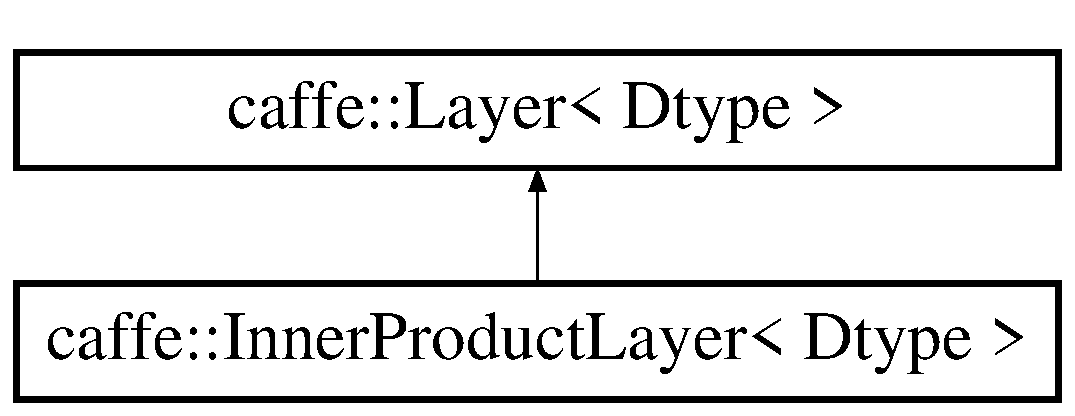
\includegraphics[height=2.000000cm]{classcaffe_1_1InnerProductLayer}
\end{center}
\end{figure}
\subsection*{Public Member Functions}
\begin{DoxyCompactItemize}
\item 
{\bfseries Inner\+Product\+Layer} (const Layer\+Parameter \&param)\hypertarget{classcaffe_1_1InnerProductLayer_a997e3c54ed0414ebcd8eec13f083af07}{}\label{classcaffe_1_1InnerProductLayer_a997e3c54ed0414ebcd8eec13f083af07}

\item 
virtual void \hyperlink{classcaffe_1_1InnerProductLayer_af9ab23bd130b6b57ae3f04e0ad714128}{Layer\+Set\+Up} (const vector$<$ \hyperlink{classcaffe_1_1Blob}{Blob}$<$ Dtype $>$ $\ast$ $>$ \&bottom, const vector$<$ \hyperlink{classcaffe_1_1Blob}{Blob}$<$ Dtype $>$ $\ast$ $>$ \&top)
\begin{DoxyCompactList}\small\item\em Does layer-\/specific setup\+: your layer should implement this function as well as Reshape. \end{DoxyCompactList}\item 
virtual void \hyperlink{classcaffe_1_1InnerProductLayer_a876806186184424573075b04281e9a72}{Reshape} (const vector$<$ \hyperlink{classcaffe_1_1Blob}{Blob}$<$ Dtype $>$ $\ast$ $>$ \&bottom, const vector$<$ \hyperlink{classcaffe_1_1Blob}{Blob}$<$ Dtype $>$ $\ast$ $>$ \&top)
\begin{DoxyCompactList}\small\item\em Adjust the shapes of top blobs and internal buffers to accommodate the shapes of the bottom blobs. \end{DoxyCompactList}\item 
virtual const char $\ast$ \hyperlink{classcaffe_1_1InnerProductLayer_a4f3a80850aa7ad5efec4fab43695a919}{type} () const \hypertarget{classcaffe_1_1InnerProductLayer_a4f3a80850aa7ad5efec4fab43695a919}{}\label{classcaffe_1_1InnerProductLayer_a4f3a80850aa7ad5efec4fab43695a919}

\begin{DoxyCompactList}\small\item\em Returns the layer type. \end{DoxyCompactList}\item 
virtual int \hyperlink{classcaffe_1_1InnerProductLayer_a53daee4cea7f8902042418a3925ee0a5}{Exact\+Num\+Bottom\+Blobs} () const 
\begin{DoxyCompactList}\small\item\em Returns the exact number of bottom blobs required by the layer, or -\/1 if no exact number is required. \end{DoxyCompactList}\item 
virtual int \hyperlink{classcaffe_1_1InnerProductLayer_a14a316bbfecc839fc65dc9c8aadc0b6d}{Exact\+Num\+Top\+Blobs} () const 
\begin{DoxyCompactList}\small\item\em Returns the exact number of top blobs required by the layer, or -\/1 if no exact number is required. \end{DoxyCompactList}\end{DoxyCompactItemize}
\subsection*{Protected Member Functions}
\begin{DoxyCompactItemize}
\item 
virtual void \hyperlink{classcaffe_1_1InnerProductLayer_af7b269821761de17e3b59180b35902f2}{Forward\+\_\+cpu} (const vector$<$ \hyperlink{classcaffe_1_1Blob}{Blob}$<$ Dtype $>$ $\ast$ $>$ \&bottom, const vector$<$ \hyperlink{classcaffe_1_1Blob}{Blob}$<$ Dtype $>$ $\ast$ $>$ \&top)\hypertarget{classcaffe_1_1InnerProductLayer_af7b269821761de17e3b59180b35902f2}{}\label{classcaffe_1_1InnerProductLayer_af7b269821761de17e3b59180b35902f2}

\begin{DoxyCompactList}\small\item\em Using the C\+PU device, compute the layer output. \end{DoxyCompactList}\item 
virtual void \hyperlink{classcaffe_1_1InnerProductLayer_a67d50ed81714f94d75d5ca0b57af38e0}{Forward\+\_\+gpu} (const vector$<$ \hyperlink{classcaffe_1_1Blob}{Blob}$<$ Dtype $>$ $\ast$ $>$ \&bottom, const vector$<$ \hyperlink{classcaffe_1_1Blob}{Blob}$<$ Dtype $>$ $\ast$ $>$ \&top)\hypertarget{classcaffe_1_1InnerProductLayer_a67d50ed81714f94d75d5ca0b57af38e0}{}\label{classcaffe_1_1InnerProductLayer_a67d50ed81714f94d75d5ca0b57af38e0}

\begin{DoxyCompactList}\small\item\em Using the G\+PU device, compute the layer output. Fall back to \hyperlink{classcaffe_1_1InnerProductLayer_af7b269821761de17e3b59180b35902f2}{Forward\+\_\+cpu()} if unavailable. \end{DoxyCompactList}\item 
virtual void \hyperlink{classcaffe_1_1InnerProductLayer_a3828d4dd2bfe3257552e5a519deb2104}{Backward\+\_\+cpu} (const vector$<$ \hyperlink{classcaffe_1_1Blob}{Blob}$<$ Dtype $>$ $\ast$ $>$ \&top, const vector$<$ bool $>$ \&propagate\+\_\+down, const vector$<$ \hyperlink{classcaffe_1_1Blob}{Blob}$<$ Dtype $>$ $\ast$ $>$ \&bottom)\hypertarget{classcaffe_1_1InnerProductLayer_a3828d4dd2bfe3257552e5a519deb2104}{}\label{classcaffe_1_1InnerProductLayer_a3828d4dd2bfe3257552e5a519deb2104}

\begin{DoxyCompactList}\small\item\em Using the C\+PU device, compute the gradients for any parameters and for the bottom blobs if propagate\+\_\+down is true. \end{DoxyCompactList}\item 
virtual void \hyperlink{classcaffe_1_1InnerProductLayer_afaccd53a581beefafede4d2b5dca98f3}{Backward\+\_\+gpu} (const vector$<$ \hyperlink{classcaffe_1_1Blob}{Blob}$<$ Dtype $>$ $\ast$ $>$ \&top, const vector$<$ bool $>$ \&propagate\+\_\+down, const vector$<$ \hyperlink{classcaffe_1_1Blob}{Blob}$<$ Dtype $>$ $\ast$ $>$ \&bottom)\hypertarget{classcaffe_1_1InnerProductLayer_afaccd53a581beefafede4d2b5dca98f3}{}\label{classcaffe_1_1InnerProductLayer_afaccd53a581beefafede4d2b5dca98f3}

\begin{DoxyCompactList}\small\item\em Using the G\+PU device, compute the gradients for any parameters and for the bottom blobs if propagate\+\_\+down is true. Fall back to \hyperlink{classcaffe_1_1InnerProductLayer_a3828d4dd2bfe3257552e5a519deb2104}{Backward\+\_\+cpu()} if unavailable. \end{DoxyCompactList}\end{DoxyCompactItemize}
\subsection*{Protected Attributes}
\begin{DoxyCompactItemize}
\item 
int {\bfseries M\+\_\+}\hypertarget{classcaffe_1_1InnerProductLayer_a7cfcde40b118c74a0e85aa3b58e8aa07}{}\label{classcaffe_1_1InnerProductLayer_a7cfcde40b118c74a0e85aa3b58e8aa07}

\item 
int {\bfseries K\+\_\+}\hypertarget{classcaffe_1_1InnerProductLayer_ad5a55ef3cb96a332977930cfaa700c66}{}\label{classcaffe_1_1InnerProductLayer_ad5a55ef3cb96a332977930cfaa700c66}

\item 
int {\bfseries N\+\_\+}\hypertarget{classcaffe_1_1InnerProductLayer_a863f699772bf8b8d978d6ec8bca42463}{}\label{classcaffe_1_1InnerProductLayer_a863f699772bf8b8d978d6ec8bca42463}

\item 
bool {\bfseries bias\+\_\+term\+\_\+}\hypertarget{classcaffe_1_1InnerProductLayer_a7193d161e30f35b3f6d23293480eb683}{}\label{classcaffe_1_1InnerProductLayer_a7193d161e30f35b3f6d23293480eb683}

\item 
\hyperlink{classcaffe_1_1Blob}{Blob}$<$ Dtype $>$ {\bfseries bias\+\_\+multiplier\+\_\+}\hypertarget{classcaffe_1_1InnerProductLayer_a5b6cf7103085b0460b64e35a0b88a137}{}\label{classcaffe_1_1InnerProductLayer_a5b6cf7103085b0460b64e35a0b88a137}

\item 
bool \hyperlink{classcaffe_1_1InnerProductLayer_a3d881acc0f3bbfb2edb37576592d5c14}{transpose\+\_\+}\hypertarget{classcaffe_1_1InnerProductLayer_a3d881acc0f3bbfb2edb37576592d5c14}{}\label{classcaffe_1_1InnerProductLayer_a3d881acc0f3bbfb2edb37576592d5c14}

\begin{DoxyCompactList}\small\item\em if true, assume transposed weights \end{DoxyCompactList}\end{DoxyCompactItemize}


\subsection{Detailed Description}
\subsubsection*{template$<$typename Dtype$>$\\*
class caffe\+::\+Inner\+Product\+Layer$<$ Dtype $>$}

Also known as a \char`\"{}fully-\/connected\char`\"{} layer, computes an inner product with a set of learned weights, and (optionally) adds biases. 

T\+O\+D\+O(dox)\+: thorough documentation for Forward, Backward, and proto params. 

\subsection{Member Function Documentation}
\index{caffe\+::\+Inner\+Product\+Layer@{caffe\+::\+Inner\+Product\+Layer}!Exact\+Num\+Bottom\+Blobs@{Exact\+Num\+Bottom\+Blobs}}
\index{Exact\+Num\+Bottom\+Blobs@{Exact\+Num\+Bottom\+Blobs}!caffe\+::\+Inner\+Product\+Layer@{caffe\+::\+Inner\+Product\+Layer}}
\subsubsection[{\texorpdfstring{Exact\+Num\+Bottom\+Blobs() const }{ExactNumBottomBlobs() const }}]{\setlength{\rightskip}{0pt plus 5cm}template$<$typename Dtype $>$ virtual int {\bf caffe\+::\+Inner\+Product\+Layer}$<$ Dtype $>$\+::Exact\+Num\+Bottom\+Blobs (
\begin{DoxyParamCaption}
{}
\end{DoxyParamCaption}
) const\hspace{0.3cm}{\ttfamily [inline]}, {\ttfamily [virtual]}}\hypertarget{classcaffe_1_1InnerProductLayer_a53daee4cea7f8902042418a3925ee0a5}{}\label{classcaffe_1_1InnerProductLayer_a53daee4cea7f8902042418a3925ee0a5}


Returns the exact number of bottom blobs required by the layer, or -\/1 if no exact number is required. 

This method should be overridden to return a non-\/negative value if your layer expects some exact number of bottom blobs. 

Reimplemented from \hyperlink{classcaffe_1_1Layer_a45c7a7943a8a6735ac433c9be11e0240}{caffe\+::\+Layer$<$ Dtype $>$}.

\index{caffe\+::\+Inner\+Product\+Layer@{caffe\+::\+Inner\+Product\+Layer}!Exact\+Num\+Top\+Blobs@{Exact\+Num\+Top\+Blobs}}
\index{Exact\+Num\+Top\+Blobs@{Exact\+Num\+Top\+Blobs}!caffe\+::\+Inner\+Product\+Layer@{caffe\+::\+Inner\+Product\+Layer}}
\subsubsection[{\texorpdfstring{Exact\+Num\+Top\+Blobs() const }{ExactNumTopBlobs() const }}]{\setlength{\rightskip}{0pt plus 5cm}template$<$typename Dtype $>$ virtual int {\bf caffe\+::\+Inner\+Product\+Layer}$<$ Dtype $>$\+::Exact\+Num\+Top\+Blobs (
\begin{DoxyParamCaption}
{}
\end{DoxyParamCaption}
) const\hspace{0.3cm}{\ttfamily [inline]}, {\ttfamily [virtual]}}\hypertarget{classcaffe_1_1InnerProductLayer_a14a316bbfecc839fc65dc9c8aadc0b6d}{}\label{classcaffe_1_1InnerProductLayer_a14a316bbfecc839fc65dc9c8aadc0b6d}


Returns the exact number of top blobs required by the layer, or -\/1 if no exact number is required. 

This method should be overridden to return a non-\/negative value if your layer expects some exact number of top blobs. 

Reimplemented from \hyperlink{classcaffe_1_1Layer_aa3c99ed707e8db683a3043412e151af8}{caffe\+::\+Layer$<$ Dtype $>$}.

\index{caffe\+::\+Inner\+Product\+Layer@{caffe\+::\+Inner\+Product\+Layer}!Layer\+Set\+Up@{Layer\+Set\+Up}}
\index{Layer\+Set\+Up@{Layer\+Set\+Up}!caffe\+::\+Inner\+Product\+Layer@{caffe\+::\+Inner\+Product\+Layer}}
\subsubsection[{\texorpdfstring{Layer\+Set\+Up(const vector$<$ Blob$<$ Dtype $>$ $\ast$ $>$ \&bottom, const vector$<$ Blob$<$ Dtype $>$ $\ast$ $>$ \&top)}{LayerSetUp(const vector< Blob< Dtype > * > &bottom, const vector< Blob< Dtype > * > &top)}}]{\setlength{\rightskip}{0pt plus 5cm}template$<$typename Dtype $>$ void {\bf caffe\+::\+Inner\+Product\+Layer}$<$ Dtype $>$\+::Layer\+Set\+Up (
\begin{DoxyParamCaption}
\item[{const vector$<$ {\bf Blob}$<$ Dtype $>$ $\ast$ $>$ \&}]{bottom, }
\item[{const vector$<$ {\bf Blob}$<$ Dtype $>$ $\ast$ $>$ \&}]{top}
\end{DoxyParamCaption}
)\hspace{0.3cm}{\ttfamily [virtual]}}\hypertarget{classcaffe_1_1InnerProductLayer_af9ab23bd130b6b57ae3f04e0ad714128}{}\label{classcaffe_1_1InnerProductLayer_af9ab23bd130b6b57ae3f04e0ad714128}


Does layer-\/specific setup\+: your layer should implement this function as well as Reshape. 


\begin{DoxyParams}{Parameters}
{\em bottom} & the preshaped input blobs, whose data fields store the input data for this layer \\
\hline
{\em top} & the allocated but unshaped output blobs\\
\hline
\end{DoxyParams}
This method should do one-\/time layer specific setup. This includes reading and processing relevent parameters from the {\ttfamily layer\+\_\+param\+\_\+}. Setting up the shapes of top blobs and internal buffers should be done in {\ttfamily Reshape}, which will be called before the forward pass to adjust the top blob sizes. 

Reimplemented from \hyperlink{classcaffe_1_1Layer_a38dc2488bf319b8de5a7ac84e0045393}{caffe\+::\+Layer$<$ Dtype $>$}.

\index{caffe\+::\+Inner\+Product\+Layer@{caffe\+::\+Inner\+Product\+Layer}!Reshape@{Reshape}}
\index{Reshape@{Reshape}!caffe\+::\+Inner\+Product\+Layer@{caffe\+::\+Inner\+Product\+Layer}}
\subsubsection[{\texorpdfstring{Reshape(const vector$<$ Blob$<$ Dtype $>$ $\ast$ $>$ \&bottom, const vector$<$ Blob$<$ Dtype $>$ $\ast$ $>$ \&top)}{Reshape(const vector< Blob< Dtype > * > &bottom, const vector< Blob< Dtype > * > &top)}}]{\setlength{\rightskip}{0pt plus 5cm}template$<$typename Dtype $>$ void {\bf caffe\+::\+Inner\+Product\+Layer}$<$ Dtype $>$\+::Reshape (
\begin{DoxyParamCaption}
\item[{const vector$<$ {\bf Blob}$<$ Dtype $>$ $\ast$ $>$ \&}]{bottom, }
\item[{const vector$<$ {\bf Blob}$<$ Dtype $>$ $\ast$ $>$ \&}]{top}
\end{DoxyParamCaption}
)\hspace{0.3cm}{\ttfamily [virtual]}}\hypertarget{classcaffe_1_1InnerProductLayer_a876806186184424573075b04281e9a72}{}\label{classcaffe_1_1InnerProductLayer_a876806186184424573075b04281e9a72}


Adjust the shapes of top blobs and internal buffers to accommodate the shapes of the bottom blobs. 


\begin{DoxyParams}{Parameters}
{\em bottom} & the input blobs, with the requested input shapes \\
\hline
{\em top} & the top blobs, which should be reshaped as needed\\
\hline
\end{DoxyParams}
This method should reshape top blobs as needed according to the shapes of the bottom (input) blobs, as well as reshaping any internal buffers and making any other necessary adjustments so that the layer can accommodate the bottom blobs. 

Implements \hyperlink{classcaffe_1_1Layer_ad9d391b972c769c0ebee34ca6d1c973e}{caffe\+::\+Layer$<$ Dtype $>$}.



The documentation for this class was generated from the following files\+:\begin{DoxyCompactItemize}
\item 
include/caffe/layers/inner\+\_\+product\+\_\+layer.\+hpp\item 
src/caffe/layers/inner\+\_\+product\+\_\+layer.\+cpp\end{DoxyCompactItemize}

\hypertarget{classcaffe_1_1InputLayer}{}\section{caffe\+:\+:Input\+Layer$<$ Dtype $>$ Class Template Reference}
\label{classcaffe_1_1InputLayer}\index{caffe\+::\+Input\+Layer$<$ Dtype $>$@{caffe\+::\+Input\+Layer$<$ Dtype $>$}}


Provides data to the \hyperlink{classcaffe_1_1Net}{Net} by assigning tops directly.  




{\ttfamily \#include $<$input\+\_\+layer.\+hpp$>$}

Inheritance diagram for caffe\+:\+:Input\+Layer$<$ Dtype $>$\+:\begin{figure}[H]
\begin{center}
\leavevmode
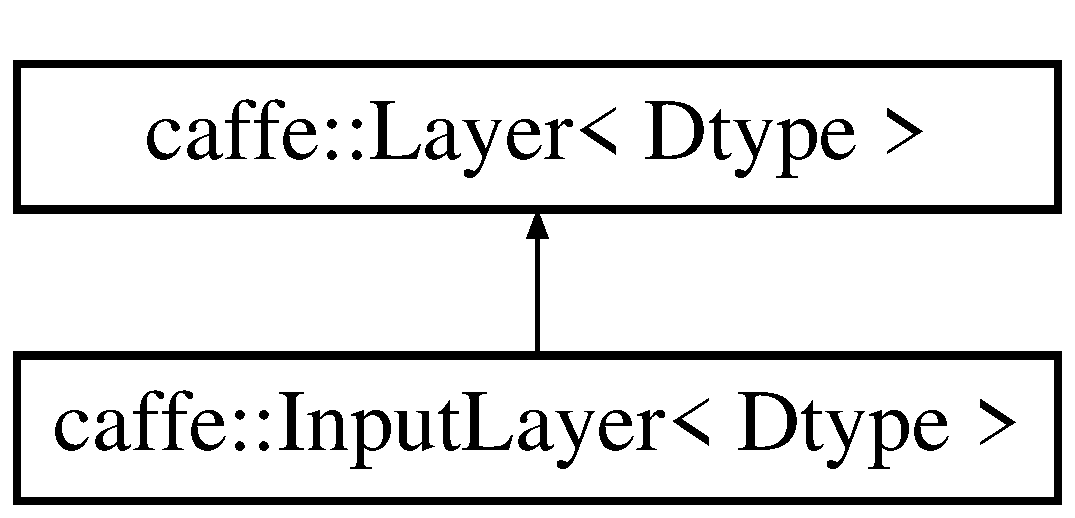
\includegraphics[height=2.000000cm]{classcaffe_1_1InputLayer}
\end{center}
\end{figure}
\subsection*{Public Member Functions}
\begin{DoxyCompactItemize}
\item 
{\bfseries Input\+Layer} (const Layer\+Parameter \&param)\hypertarget{classcaffe_1_1InputLayer_af95727fa25481ed69eb93fb05336e4d8}{}\label{classcaffe_1_1InputLayer_af95727fa25481ed69eb93fb05336e4d8}

\item 
virtual void \hyperlink{classcaffe_1_1InputLayer_afafb49133e9d87ce6f67fc4a12ca1fb3}{Layer\+Set\+Up} (const vector$<$ \hyperlink{classcaffe_1_1Blob}{Blob}$<$ Dtype $>$ $\ast$ $>$ \&bottom, const vector$<$ \hyperlink{classcaffe_1_1Blob}{Blob}$<$ Dtype $>$ $\ast$ $>$ \&top)
\begin{DoxyCompactList}\small\item\em Does layer-\/specific setup\+: your layer should implement this function as well as Reshape. \end{DoxyCompactList}\item 
virtual void \hyperlink{classcaffe_1_1InputLayer_aae5f93f3456b0392d6145ae8c2d7d98e}{Reshape} (const vector$<$ \hyperlink{classcaffe_1_1Blob}{Blob}$<$ Dtype $>$ $\ast$ $>$ \&bottom, const vector$<$ \hyperlink{classcaffe_1_1Blob}{Blob}$<$ Dtype $>$ $\ast$ $>$ \&top)
\begin{DoxyCompactList}\small\item\em Adjust the shapes of top blobs and internal buffers to accommodate the shapes of the bottom blobs. \end{DoxyCompactList}\item 
virtual const char $\ast$ \hyperlink{classcaffe_1_1InputLayer_a809104dd51ae8c0343ddd9027f0392d1}{type} () const \hypertarget{classcaffe_1_1InputLayer_a809104dd51ae8c0343ddd9027f0392d1}{}\label{classcaffe_1_1InputLayer_a809104dd51ae8c0343ddd9027f0392d1}

\begin{DoxyCompactList}\small\item\em Returns the layer type. \end{DoxyCompactList}\item 
virtual int \hyperlink{classcaffe_1_1InputLayer_a5bb058da95fd98a74385bbd3eccbe56b}{Exact\+Num\+Bottom\+Blobs} () const 
\begin{DoxyCompactList}\small\item\em Returns the exact number of bottom blobs required by the layer, or -\/1 if no exact number is required. \end{DoxyCompactList}\item 
virtual int \hyperlink{classcaffe_1_1InputLayer_a32e355fd419a6144aedf3a91843a8089}{Min\+Top\+Blobs} () const 
\begin{DoxyCompactList}\small\item\em Returns the minimum number of top blobs required by the layer, or -\/1 if no minimum number is required. \end{DoxyCompactList}\end{DoxyCompactItemize}
\subsection*{Protected Member Functions}
\begin{DoxyCompactItemize}
\item 
virtual void \hyperlink{classcaffe_1_1InputLayer_aaa8f0afa0e900adb9e05153d7b728345}{Forward\+\_\+cpu} (const vector$<$ \hyperlink{classcaffe_1_1Blob}{Blob}$<$ Dtype $>$ $\ast$ $>$ \&bottom, const vector$<$ \hyperlink{classcaffe_1_1Blob}{Blob}$<$ Dtype $>$ $\ast$ $>$ \&top)\hypertarget{classcaffe_1_1InputLayer_aaa8f0afa0e900adb9e05153d7b728345}{}\label{classcaffe_1_1InputLayer_aaa8f0afa0e900adb9e05153d7b728345}

\begin{DoxyCompactList}\small\item\em Using the C\+PU device, compute the layer output. \end{DoxyCompactList}\item 
virtual void \hyperlink{classcaffe_1_1InputLayer_a0a53bdde1a21d5f10319054ca0e9839d}{Backward\+\_\+cpu} (const vector$<$ \hyperlink{classcaffe_1_1Blob}{Blob}$<$ Dtype $>$ $\ast$ $>$ \&top, const vector$<$ bool $>$ \&propagate\+\_\+down, const vector$<$ \hyperlink{classcaffe_1_1Blob}{Blob}$<$ Dtype $>$ $\ast$ $>$ \&bottom)\hypertarget{classcaffe_1_1InputLayer_a0a53bdde1a21d5f10319054ca0e9839d}{}\label{classcaffe_1_1InputLayer_a0a53bdde1a21d5f10319054ca0e9839d}

\begin{DoxyCompactList}\small\item\em Using the C\+PU device, compute the gradients for any parameters and for the bottom blobs if propagate\+\_\+down is true. \end{DoxyCompactList}\end{DoxyCompactItemize}
\subsection*{Additional Inherited Members}


\subsection{Detailed Description}
\subsubsection*{template$<$typename Dtype$>$\\*
class caffe\+::\+Input\+Layer$<$ Dtype $>$}

Provides data to the \hyperlink{classcaffe_1_1Net}{Net} by assigning tops directly. 

This data layer is a container that merely holds the data assigned to it; forward, backward, and reshape are all no-\/ops. 

\subsection{Member Function Documentation}
\index{caffe\+::\+Input\+Layer@{caffe\+::\+Input\+Layer}!Exact\+Num\+Bottom\+Blobs@{Exact\+Num\+Bottom\+Blobs}}
\index{Exact\+Num\+Bottom\+Blobs@{Exact\+Num\+Bottom\+Blobs}!caffe\+::\+Input\+Layer@{caffe\+::\+Input\+Layer}}
\subsubsection[{\texorpdfstring{Exact\+Num\+Bottom\+Blobs() const }{ExactNumBottomBlobs() const }}]{\setlength{\rightskip}{0pt plus 5cm}template$<$typename Dtype $>$ virtual int {\bf caffe\+::\+Input\+Layer}$<$ Dtype $>$\+::Exact\+Num\+Bottom\+Blobs (
\begin{DoxyParamCaption}
{}
\end{DoxyParamCaption}
) const\hspace{0.3cm}{\ttfamily [inline]}, {\ttfamily [virtual]}}\hypertarget{classcaffe_1_1InputLayer_a5bb058da95fd98a74385bbd3eccbe56b}{}\label{classcaffe_1_1InputLayer_a5bb058da95fd98a74385bbd3eccbe56b}


Returns the exact number of bottom blobs required by the layer, or -\/1 if no exact number is required. 

This method should be overridden to return a non-\/negative value if your layer expects some exact number of bottom blobs. 

Reimplemented from \hyperlink{classcaffe_1_1Layer_a45c7a7943a8a6735ac433c9be11e0240}{caffe\+::\+Layer$<$ Dtype $>$}.

\index{caffe\+::\+Input\+Layer@{caffe\+::\+Input\+Layer}!Layer\+Set\+Up@{Layer\+Set\+Up}}
\index{Layer\+Set\+Up@{Layer\+Set\+Up}!caffe\+::\+Input\+Layer@{caffe\+::\+Input\+Layer}}
\subsubsection[{\texorpdfstring{Layer\+Set\+Up(const vector$<$ Blob$<$ Dtype $>$ $\ast$ $>$ \&bottom, const vector$<$ Blob$<$ Dtype $>$ $\ast$ $>$ \&top)}{LayerSetUp(const vector< Blob< Dtype > * > &bottom, const vector< Blob< Dtype > * > &top)}}]{\setlength{\rightskip}{0pt plus 5cm}template$<$typename Dtype $>$ void {\bf caffe\+::\+Input\+Layer}$<$ Dtype $>$\+::Layer\+Set\+Up (
\begin{DoxyParamCaption}
\item[{const vector$<$ {\bf Blob}$<$ Dtype $>$ $\ast$ $>$ \&}]{bottom, }
\item[{const vector$<$ {\bf Blob}$<$ Dtype $>$ $\ast$ $>$ \&}]{top}
\end{DoxyParamCaption}
)\hspace{0.3cm}{\ttfamily [virtual]}}\hypertarget{classcaffe_1_1InputLayer_afafb49133e9d87ce6f67fc4a12ca1fb3}{}\label{classcaffe_1_1InputLayer_afafb49133e9d87ce6f67fc4a12ca1fb3}


Does layer-\/specific setup\+: your layer should implement this function as well as Reshape. 


\begin{DoxyParams}{Parameters}
{\em bottom} & the preshaped input blobs, whose data fields store the input data for this layer \\
\hline
{\em top} & the allocated but unshaped output blobs\\
\hline
\end{DoxyParams}
This method should do one-\/time layer specific setup. This includes reading and processing relevent parameters from the {\ttfamily layer\+\_\+param\+\_\+}. Setting up the shapes of top blobs and internal buffers should be done in {\ttfamily Reshape}, which will be called before the forward pass to adjust the top blob sizes. 

Reimplemented from \hyperlink{classcaffe_1_1Layer_a38dc2488bf319b8de5a7ac84e0045393}{caffe\+::\+Layer$<$ Dtype $>$}.

\index{caffe\+::\+Input\+Layer@{caffe\+::\+Input\+Layer}!Min\+Top\+Blobs@{Min\+Top\+Blobs}}
\index{Min\+Top\+Blobs@{Min\+Top\+Blobs}!caffe\+::\+Input\+Layer@{caffe\+::\+Input\+Layer}}
\subsubsection[{\texorpdfstring{Min\+Top\+Blobs() const }{MinTopBlobs() const }}]{\setlength{\rightskip}{0pt plus 5cm}template$<$typename Dtype $>$ virtual int {\bf caffe\+::\+Input\+Layer}$<$ Dtype $>$\+::Min\+Top\+Blobs (
\begin{DoxyParamCaption}
{}
\end{DoxyParamCaption}
) const\hspace{0.3cm}{\ttfamily [inline]}, {\ttfamily [virtual]}}\hypertarget{classcaffe_1_1InputLayer_a32e355fd419a6144aedf3a91843a8089}{}\label{classcaffe_1_1InputLayer_a32e355fd419a6144aedf3a91843a8089}


Returns the minimum number of top blobs required by the layer, or -\/1 if no minimum number is required. 

This method should be overridden to return a non-\/negative value if your layer expects some minimum number of top blobs. 

Reimplemented from \hyperlink{classcaffe_1_1Layer_a8bb143d58a740345fa2dc3d4204d553b}{caffe\+::\+Layer$<$ Dtype $>$}.

\index{caffe\+::\+Input\+Layer@{caffe\+::\+Input\+Layer}!Reshape@{Reshape}}
\index{Reshape@{Reshape}!caffe\+::\+Input\+Layer@{caffe\+::\+Input\+Layer}}
\subsubsection[{\texorpdfstring{Reshape(const vector$<$ Blob$<$ Dtype $>$ $\ast$ $>$ \&bottom, const vector$<$ Blob$<$ Dtype $>$ $\ast$ $>$ \&top)}{Reshape(const vector< Blob< Dtype > * > &bottom, const vector< Blob< Dtype > * > &top)}}]{\setlength{\rightskip}{0pt plus 5cm}template$<$typename Dtype $>$ virtual void {\bf caffe\+::\+Input\+Layer}$<$ Dtype $>$\+::Reshape (
\begin{DoxyParamCaption}
\item[{const vector$<$ {\bf Blob}$<$ Dtype $>$ $\ast$ $>$ \&}]{bottom, }
\item[{const vector$<$ {\bf Blob}$<$ Dtype $>$ $\ast$ $>$ \&}]{top}
\end{DoxyParamCaption}
)\hspace{0.3cm}{\ttfamily [inline]}, {\ttfamily [virtual]}}\hypertarget{classcaffe_1_1InputLayer_aae5f93f3456b0392d6145ae8c2d7d98e}{}\label{classcaffe_1_1InputLayer_aae5f93f3456b0392d6145ae8c2d7d98e}


Adjust the shapes of top blobs and internal buffers to accommodate the shapes of the bottom blobs. 


\begin{DoxyParams}{Parameters}
{\em bottom} & the input blobs, with the requested input shapes \\
\hline
{\em top} & the top blobs, which should be reshaped as needed\\
\hline
\end{DoxyParams}
This method should reshape top blobs as needed according to the shapes of the bottom (input) blobs, as well as reshaping any internal buffers and making any other necessary adjustments so that the layer can accommodate the bottom blobs. 

Implements \hyperlink{classcaffe_1_1Layer_ad9d391b972c769c0ebee34ca6d1c973e}{caffe\+::\+Layer$<$ Dtype $>$}.



The documentation for this class was generated from the following files\+:\begin{DoxyCompactItemize}
\item 
include/caffe/layers/input\+\_\+layer.\+hpp\item 
src/caffe/layers/input\+\_\+layer.\+cpp\end{DoxyCompactItemize}

\hypertarget{classcaffe_1_1InternalThread}{}\section{caffe\+:\+:Internal\+Thread Class Reference}
\label{classcaffe_1_1InternalThread}\index{caffe\+::\+Internal\+Thread@{caffe\+::\+Internal\+Thread}}


{\ttfamily \#include $<$internal\+\_\+thread.\+hpp$>$}

Inheritance diagram for caffe\+:\+:Internal\+Thread\+:\begin{figure}[H]
\begin{center}
\leavevmode
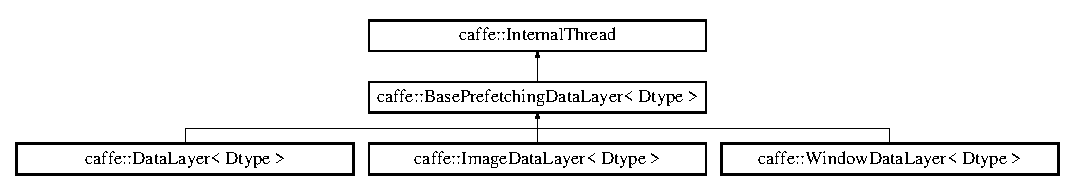
\includegraphics[height=2.121212cm]{classcaffe_1_1InternalThread}
\end{center}
\end{figure}
\subsection*{Public Member Functions}
\begin{DoxyCompactItemize}
\item 
void \hyperlink{classcaffe_1_1InternalThread_acffc1d9bc9e78f4146ba2d16f593fca7}{Start\+Internal\+Thread} ()
\item 
void \hyperlink{classcaffe_1_1InternalThread_ac72d8e2a23dbbe5203d5003dd67af73e}{Stop\+Internal\+Thread} ()
\item 
bool {\bfseries is\+\_\+started} () const \hypertarget{classcaffe_1_1InternalThread_a6c452462793500206228c69de8b6758c}{}\label{classcaffe_1_1InternalThread_a6c452462793500206228c69de8b6758c}

\end{DoxyCompactItemize}
\subsection*{Protected Member Functions}
\begin{DoxyCompactItemize}
\item 
virtual void {\bfseries Internal\+Thread\+Entry} ()\hypertarget{classcaffe_1_1InternalThread_a40b9506bc2985fdc189cff4fa680880b}{}\label{classcaffe_1_1InternalThread_a40b9506bc2985fdc189cff4fa680880b}

\item 
bool {\bfseries must\+\_\+stop} ()\hypertarget{classcaffe_1_1InternalThread_a16fd45781962d8f59556b9323f11a397}{}\label{classcaffe_1_1InternalThread_a16fd45781962d8f59556b9323f11a397}

\end{DoxyCompactItemize}


\subsection{Detailed Description}
Virtual class encapsulate boost\+::thread for use in base class The child class will acquire the ability to run a single thread, by reimplementing the virtual function Internal\+Thread\+Entry. 

\subsection{Member Function Documentation}
\index{caffe\+::\+Internal\+Thread@{caffe\+::\+Internal\+Thread}!Start\+Internal\+Thread@{Start\+Internal\+Thread}}
\index{Start\+Internal\+Thread@{Start\+Internal\+Thread}!caffe\+::\+Internal\+Thread@{caffe\+::\+Internal\+Thread}}
\subsubsection[{\texorpdfstring{Start\+Internal\+Thread()}{StartInternalThread()}}]{\setlength{\rightskip}{0pt plus 5cm}void caffe\+::\+Internal\+Thread\+::\+Start\+Internal\+Thread (
\begin{DoxyParamCaption}
{}
\end{DoxyParamCaption}
)}\hypertarget{classcaffe_1_1InternalThread_acffc1d9bc9e78f4146ba2d16f593fca7}{}\label{classcaffe_1_1InternalThread_acffc1d9bc9e78f4146ba2d16f593fca7}
\hyperlink{classcaffe_1_1Caffe}{Caffe}\textquotesingle{}s thread local state will be initialized using the current thread values, e.\+g. device id, solver index etc. The random seed is initialized using caffe\+\_\+rng\+\_\+rand. \index{caffe\+::\+Internal\+Thread@{caffe\+::\+Internal\+Thread}!Stop\+Internal\+Thread@{Stop\+Internal\+Thread}}
\index{Stop\+Internal\+Thread@{Stop\+Internal\+Thread}!caffe\+::\+Internal\+Thread@{caffe\+::\+Internal\+Thread}}
\subsubsection[{\texorpdfstring{Stop\+Internal\+Thread()}{StopInternalThread()}}]{\setlength{\rightskip}{0pt plus 5cm}void caffe\+::\+Internal\+Thread\+::\+Stop\+Internal\+Thread (
\begin{DoxyParamCaption}
{}
\end{DoxyParamCaption}
)}\hypertarget{classcaffe_1_1InternalThread_ac72d8e2a23dbbe5203d5003dd67af73e}{}\label{classcaffe_1_1InternalThread_ac72d8e2a23dbbe5203d5003dd67af73e}
Will not return until the internal thread has exited. 

The documentation for this class was generated from the following files\+:\begin{DoxyCompactItemize}
\item 
include/caffe/internal\+\_\+thread.\+hpp\item 
src/caffe/internal\+\_\+thread.\+cpp\end{DoxyCompactItemize}

\hypertarget{classcaffe_1_1InterpLayer}{}\section{caffe\+:\+:Interp\+Layer$<$ Dtype $>$ Class Template Reference}
\label{classcaffe_1_1InterpLayer}\index{caffe\+::\+Interp\+Layer$<$ Dtype $>$@{caffe\+::\+Interp\+Layer$<$ Dtype $>$}}


Changes the spatial resolution by bi-\/linear interpolation. The target size is specified in terms of pixels. The start and end pixels of the input are mapped to the start and end pixels of the output.  




{\ttfamily \#include $<$interp\+\_\+layer.\+hpp$>$}

Inheritance diagram for caffe\+:\+:Interp\+Layer$<$ Dtype $>$\+:\begin{figure}[H]
\begin{center}
\leavevmode
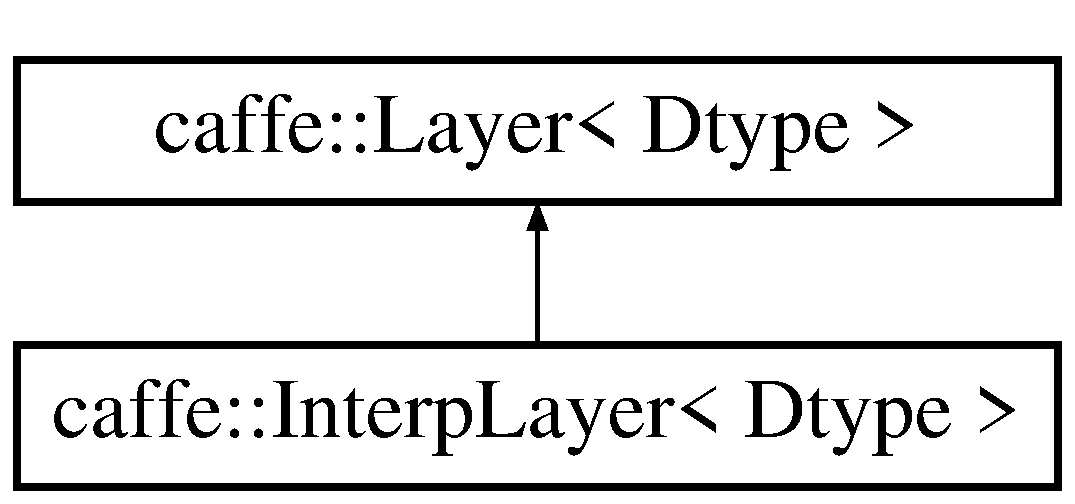
\includegraphics[height=2.000000cm]{classcaffe_1_1InterpLayer}
\end{center}
\end{figure}
\subsection*{Public Member Functions}
\begin{DoxyCompactItemize}
\item 
{\bfseries Interp\+Layer} (const Layer\+Parameter \&param)\hypertarget{classcaffe_1_1InterpLayer_a23b9c18e3e251c4f3e471303e11f3250}{}\label{classcaffe_1_1InterpLayer_a23b9c18e3e251c4f3e471303e11f3250}

\item 
virtual void \hyperlink{classcaffe_1_1InterpLayer_ac8f4627f1a04fa8d3e85eaac5f1fa291}{Layer\+Set\+Up} (const vector$<$ \hyperlink{classcaffe_1_1Blob}{Blob}$<$ Dtype $>$ $\ast$ $>$ \&bottom, const vector$<$ \hyperlink{classcaffe_1_1Blob}{Blob}$<$ Dtype $>$ $\ast$ $>$ \&top)
\begin{DoxyCompactList}\small\item\em Does layer-\/specific setup\+: your layer should implement this function as well as Reshape. \end{DoxyCompactList}\item 
virtual void \hyperlink{classcaffe_1_1InterpLayer_a738a790541cf3f1827afa9f71b835caa}{Reshape} (const vector$<$ \hyperlink{classcaffe_1_1Blob}{Blob}$<$ Dtype $>$ $\ast$ $>$ \&bottom, const vector$<$ \hyperlink{classcaffe_1_1Blob}{Blob}$<$ Dtype $>$ $\ast$ $>$ \&top)
\begin{DoxyCompactList}\small\item\em Adjust the shapes of top blobs and internal buffers to accommodate the shapes of the bottom blobs. \end{DoxyCompactList}\item 
virtual const char $\ast$ \hyperlink{classcaffe_1_1InterpLayer_af23cf9dac90fb66c89bed793d49874f3}{type} () const \hypertarget{classcaffe_1_1InterpLayer_af23cf9dac90fb66c89bed793d49874f3}{}\label{classcaffe_1_1InterpLayer_af23cf9dac90fb66c89bed793d49874f3}

\begin{DoxyCompactList}\small\item\em Returns the layer type. \end{DoxyCompactList}\item 
virtual int \hyperlink{classcaffe_1_1InterpLayer_a186c0c177d96da2dce60308d78959c2b}{Exact\+Num\+Bottom\+Blobs} () const 
\begin{DoxyCompactList}\small\item\em Returns the exact number of bottom blobs required by the layer, or -\/1 if no exact number is required. \end{DoxyCompactList}\item 
virtual int \hyperlink{classcaffe_1_1InterpLayer_a14e1a12b196cd87eef112d7a87d5e75e}{Exact\+Num\+Top\+Blobs} () const 
\begin{DoxyCompactList}\small\item\em Returns the exact number of top blobs required by the layer, or -\/1 if no exact number is required. \end{DoxyCompactList}\end{DoxyCompactItemize}
\subsection*{Protected Member Functions}
\begin{DoxyCompactItemize}
\item 
virtual void \hyperlink{classcaffe_1_1InterpLayer_a34b4e9bebcdcf233747184833dd6ac0e}{Forward\+\_\+cpu} (const vector$<$ \hyperlink{classcaffe_1_1Blob}{Blob}$<$ Dtype $>$ $\ast$ $>$ \&bottom, const vector$<$ \hyperlink{classcaffe_1_1Blob}{Blob}$<$ Dtype $>$ $\ast$ $>$ \&top)\hypertarget{classcaffe_1_1InterpLayer_a34b4e9bebcdcf233747184833dd6ac0e}{}\label{classcaffe_1_1InterpLayer_a34b4e9bebcdcf233747184833dd6ac0e}

\begin{DoxyCompactList}\small\item\em Using the C\+PU device, compute the layer output. \end{DoxyCompactList}\item 
virtual void \hyperlink{classcaffe_1_1InterpLayer_a980e586af1f74c44967f547d5b43c17c}{Forward\+\_\+gpu} (const vector$<$ \hyperlink{classcaffe_1_1Blob}{Blob}$<$ Dtype $>$ $\ast$ $>$ \&bottom, const vector$<$ \hyperlink{classcaffe_1_1Blob}{Blob}$<$ Dtype $>$ $\ast$ $>$ \&top)\hypertarget{classcaffe_1_1InterpLayer_a980e586af1f74c44967f547d5b43c17c}{}\label{classcaffe_1_1InterpLayer_a980e586af1f74c44967f547d5b43c17c}

\begin{DoxyCompactList}\small\item\em Using the G\+PU device, compute the layer output. Fall back to \hyperlink{classcaffe_1_1InterpLayer_a34b4e9bebcdcf233747184833dd6ac0e}{Forward\+\_\+cpu()} if unavailable. \end{DoxyCompactList}\item 
virtual void \hyperlink{classcaffe_1_1InterpLayer_a968eb0a3ad8875fb584a8ff01c66de35}{Backward\+\_\+cpu} (const vector$<$ \hyperlink{classcaffe_1_1Blob}{Blob}$<$ Dtype $>$ $\ast$ $>$ \&top, const vector$<$ bool $>$ \&propagate\+\_\+down, const vector$<$ \hyperlink{classcaffe_1_1Blob}{Blob}$<$ Dtype $>$ $\ast$ $>$ \&bottom)\hypertarget{classcaffe_1_1InterpLayer_a968eb0a3ad8875fb584a8ff01c66de35}{}\label{classcaffe_1_1InterpLayer_a968eb0a3ad8875fb584a8ff01c66de35}

\begin{DoxyCompactList}\small\item\em Using the C\+PU device, compute the gradients for any parameters and for the bottom blobs if propagate\+\_\+down is true. \end{DoxyCompactList}\item 
virtual void \hyperlink{classcaffe_1_1InterpLayer_a0414efd5b6358e5f57a4584146475157}{Backward\+\_\+gpu} (const vector$<$ \hyperlink{classcaffe_1_1Blob}{Blob}$<$ Dtype $>$ $\ast$ $>$ \&top, const vector$<$ bool $>$ \&propagate\+\_\+down, const vector$<$ \hyperlink{classcaffe_1_1Blob}{Blob}$<$ Dtype $>$ $\ast$ $>$ \&bottom)\hypertarget{classcaffe_1_1InterpLayer_a0414efd5b6358e5f57a4584146475157}{}\label{classcaffe_1_1InterpLayer_a0414efd5b6358e5f57a4584146475157}

\begin{DoxyCompactList}\small\item\em Using the G\+PU device, compute the gradients for any parameters and for the bottom blobs if propagate\+\_\+down is true. Fall back to \hyperlink{classcaffe_1_1InterpLayer_a968eb0a3ad8875fb584a8ff01c66de35}{Backward\+\_\+cpu()} if unavailable. \end{DoxyCompactList}\end{DoxyCompactItemize}
\subsection*{Protected Attributes}
\begin{DoxyCompactItemize}
\item 
int {\bfseries num\+\_\+}\hypertarget{classcaffe_1_1InterpLayer_a5f72bd111cf142dbcaf87a86f54f202b}{}\label{classcaffe_1_1InterpLayer_a5f72bd111cf142dbcaf87a86f54f202b}

\item 
int {\bfseries channels\+\_\+}\hypertarget{classcaffe_1_1InterpLayer_a9e19fb656adcbee9dd2b068750f14e0f}{}\label{classcaffe_1_1InterpLayer_a9e19fb656adcbee9dd2b068750f14e0f}

\item 
int {\bfseries height\+\_\+in\+\_\+}\hypertarget{classcaffe_1_1InterpLayer_a83a605d3049ea90e65fc4c7624234f0a}{}\label{classcaffe_1_1InterpLayer_a83a605d3049ea90e65fc4c7624234f0a}

\item 
int {\bfseries width\+\_\+in\+\_\+}\hypertarget{classcaffe_1_1InterpLayer_a4367548d13a21b39bc205f7a8531b1ad}{}\label{classcaffe_1_1InterpLayer_a4367548d13a21b39bc205f7a8531b1ad}

\item 
int {\bfseries height\+\_\+out\+\_\+}\hypertarget{classcaffe_1_1InterpLayer_a4625f8e427b9acdeaa4e3792cbbf9648}{}\label{classcaffe_1_1InterpLayer_a4625f8e427b9acdeaa4e3792cbbf9648}

\item 
int {\bfseries width\+\_\+out\+\_\+}\hypertarget{classcaffe_1_1InterpLayer_a02c2c7a789cb27a6bf9b078056b3c22f}{}\label{classcaffe_1_1InterpLayer_a02c2c7a789cb27a6bf9b078056b3c22f}

\item 
int {\bfseries pad\+\_\+beg\+\_\+}\hypertarget{classcaffe_1_1InterpLayer_a8371c85539d8d1cbcb01f6613fe1dceb}{}\label{classcaffe_1_1InterpLayer_a8371c85539d8d1cbcb01f6613fe1dceb}

\item 
int {\bfseries pad\+\_\+end\+\_\+}\hypertarget{classcaffe_1_1InterpLayer_aecf59429a6f50088b585b5517a4879e4}{}\label{classcaffe_1_1InterpLayer_aecf59429a6f50088b585b5517a4879e4}

\item 
int {\bfseries height\+\_\+in\+\_\+eff\+\_\+}\hypertarget{classcaffe_1_1InterpLayer_a5461810dc198e24db499498b0770f69a}{}\label{classcaffe_1_1InterpLayer_a5461810dc198e24db499498b0770f69a}

\item 
int {\bfseries width\+\_\+in\+\_\+eff\+\_\+}\hypertarget{classcaffe_1_1InterpLayer_a4b167fa7b9cdd6375f10849cd63a6859}{}\label{classcaffe_1_1InterpLayer_a4b167fa7b9cdd6375f10849cd63a6859}

\end{DoxyCompactItemize}


\subsection{Detailed Description}
\subsubsection*{template$<$typename Dtype$>$\\*
class caffe\+::\+Interp\+Layer$<$ Dtype $>$}

Changes the spatial resolution by bi-\/linear interpolation. The target size is specified in terms of pixels. The start and end pixels of the input are mapped to the start and end pixels of the output. 

\subsection{Member Function Documentation}
\index{caffe\+::\+Interp\+Layer@{caffe\+::\+Interp\+Layer}!Exact\+Num\+Bottom\+Blobs@{Exact\+Num\+Bottom\+Blobs}}
\index{Exact\+Num\+Bottom\+Blobs@{Exact\+Num\+Bottom\+Blobs}!caffe\+::\+Interp\+Layer@{caffe\+::\+Interp\+Layer}}
\subsubsection[{\texorpdfstring{Exact\+Num\+Bottom\+Blobs() const }{ExactNumBottomBlobs() const }}]{\setlength{\rightskip}{0pt plus 5cm}template$<$typename Dtype $>$ virtual int {\bf caffe\+::\+Interp\+Layer}$<$ Dtype $>$\+::Exact\+Num\+Bottom\+Blobs (
\begin{DoxyParamCaption}
{}
\end{DoxyParamCaption}
) const\hspace{0.3cm}{\ttfamily [inline]}, {\ttfamily [virtual]}}\hypertarget{classcaffe_1_1InterpLayer_a186c0c177d96da2dce60308d78959c2b}{}\label{classcaffe_1_1InterpLayer_a186c0c177d96da2dce60308d78959c2b}


Returns the exact number of bottom blobs required by the layer, or -\/1 if no exact number is required. 

This method should be overridden to return a non-\/negative value if your layer expects some exact number of bottom blobs. 

Reimplemented from \hyperlink{classcaffe_1_1Layer_a45c7a7943a8a6735ac433c9be11e0240}{caffe\+::\+Layer$<$ Dtype $>$}.

\index{caffe\+::\+Interp\+Layer@{caffe\+::\+Interp\+Layer}!Exact\+Num\+Top\+Blobs@{Exact\+Num\+Top\+Blobs}}
\index{Exact\+Num\+Top\+Blobs@{Exact\+Num\+Top\+Blobs}!caffe\+::\+Interp\+Layer@{caffe\+::\+Interp\+Layer}}
\subsubsection[{\texorpdfstring{Exact\+Num\+Top\+Blobs() const }{ExactNumTopBlobs() const }}]{\setlength{\rightskip}{0pt plus 5cm}template$<$typename Dtype $>$ virtual int {\bf caffe\+::\+Interp\+Layer}$<$ Dtype $>$\+::Exact\+Num\+Top\+Blobs (
\begin{DoxyParamCaption}
{}
\end{DoxyParamCaption}
) const\hspace{0.3cm}{\ttfamily [inline]}, {\ttfamily [virtual]}}\hypertarget{classcaffe_1_1InterpLayer_a14e1a12b196cd87eef112d7a87d5e75e}{}\label{classcaffe_1_1InterpLayer_a14e1a12b196cd87eef112d7a87d5e75e}


Returns the exact number of top blobs required by the layer, or -\/1 if no exact number is required. 

This method should be overridden to return a non-\/negative value if your layer expects some exact number of top blobs. 

Reimplemented from \hyperlink{classcaffe_1_1Layer_aa3c99ed707e8db683a3043412e151af8}{caffe\+::\+Layer$<$ Dtype $>$}.

\index{caffe\+::\+Interp\+Layer@{caffe\+::\+Interp\+Layer}!Layer\+Set\+Up@{Layer\+Set\+Up}}
\index{Layer\+Set\+Up@{Layer\+Set\+Up}!caffe\+::\+Interp\+Layer@{caffe\+::\+Interp\+Layer}}
\subsubsection[{\texorpdfstring{Layer\+Set\+Up(const vector$<$ Blob$<$ Dtype $>$ $\ast$ $>$ \&bottom, const vector$<$ Blob$<$ Dtype $>$ $\ast$ $>$ \&top)}{LayerSetUp(const vector< Blob< Dtype > * > &bottom, const vector< Blob< Dtype > * > &top)}}]{\setlength{\rightskip}{0pt plus 5cm}template$<$typename Dtype $>$ void {\bf caffe\+::\+Interp\+Layer}$<$ Dtype $>$\+::Layer\+Set\+Up (
\begin{DoxyParamCaption}
\item[{const vector$<$ {\bf Blob}$<$ Dtype $>$ $\ast$ $>$ \&}]{bottom, }
\item[{const vector$<$ {\bf Blob}$<$ Dtype $>$ $\ast$ $>$ \&}]{top}
\end{DoxyParamCaption}
)\hspace{0.3cm}{\ttfamily [virtual]}}\hypertarget{classcaffe_1_1InterpLayer_ac8f4627f1a04fa8d3e85eaac5f1fa291}{}\label{classcaffe_1_1InterpLayer_ac8f4627f1a04fa8d3e85eaac5f1fa291}


Does layer-\/specific setup\+: your layer should implement this function as well as Reshape. 


\begin{DoxyParams}{Parameters}
{\em bottom} & the preshaped input blobs, whose data fields store the input data for this layer \\
\hline
{\em top} & the allocated but unshaped output blobs\\
\hline
\end{DoxyParams}
This method should do one-\/time layer specific setup. This includes reading and processing relevent parameters from the {\ttfamily layer\+\_\+param\+\_\+}. Setting up the shapes of top blobs and internal buffers should be done in {\ttfamily Reshape}, which will be called before the forward pass to adjust the top blob sizes. 

Reimplemented from \hyperlink{classcaffe_1_1Layer_a38dc2488bf319b8de5a7ac84e0045393}{caffe\+::\+Layer$<$ Dtype $>$}.

\index{caffe\+::\+Interp\+Layer@{caffe\+::\+Interp\+Layer}!Reshape@{Reshape}}
\index{Reshape@{Reshape}!caffe\+::\+Interp\+Layer@{caffe\+::\+Interp\+Layer}}
\subsubsection[{\texorpdfstring{Reshape(const vector$<$ Blob$<$ Dtype $>$ $\ast$ $>$ \&bottom, const vector$<$ Blob$<$ Dtype $>$ $\ast$ $>$ \&top)}{Reshape(const vector< Blob< Dtype > * > &bottom, const vector< Blob< Dtype > * > &top)}}]{\setlength{\rightskip}{0pt plus 5cm}template$<$typename Dtype $>$ void {\bf caffe\+::\+Interp\+Layer}$<$ Dtype $>$\+::Reshape (
\begin{DoxyParamCaption}
\item[{const vector$<$ {\bf Blob}$<$ Dtype $>$ $\ast$ $>$ \&}]{bottom, }
\item[{const vector$<$ {\bf Blob}$<$ Dtype $>$ $\ast$ $>$ \&}]{top}
\end{DoxyParamCaption}
)\hspace{0.3cm}{\ttfamily [virtual]}}\hypertarget{classcaffe_1_1InterpLayer_a738a790541cf3f1827afa9f71b835caa}{}\label{classcaffe_1_1InterpLayer_a738a790541cf3f1827afa9f71b835caa}


Adjust the shapes of top blobs and internal buffers to accommodate the shapes of the bottom blobs. 


\begin{DoxyParams}{Parameters}
{\em bottom} & the input blobs, with the requested input shapes \\
\hline
{\em top} & the top blobs, which should be reshaped as needed\\
\hline
\end{DoxyParams}
This method should reshape top blobs as needed according to the shapes of the bottom (input) blobs, as well as reshaping any internal buffers and making any other necessary adjustments so that the layer can accommodate the bottom blobs. 

Implements \hyperlink{classcaffe_1_1Layer_ad9d391b972c769c0ebee34ca6d1c973e}{caffe\+::\+Layer$<$ Dtype $>$}.



The documentation for this class was generated from the following files\+:\begin{DoxyCompactItemize}
\item 
include/caffe/layers/interp\+\_\+layer.\+hpp\item 
src/caffe/layers/interp\+\_\+layer.\+cpp\end{DoxyCompactItemize}

\hypertarget{classcaffe_1_1Layer}{}\section{caffe\+:\+:Layer$<$ Dtype $>$ Class Template Reference}
\label{classcaffe_1_1Layer}\index{caffe\+::\+Layer$<$ Dtype $>$@{caffe\+::\+Layer$<$ Dtype $>$}}


An interface for the units of computation which can be composed into a \hyperlink{classcaffe_1_1Net}{Net}.  




{\ttfamily \#include $<$layer.\+hpp$>$}

Inheritance diagram for caffe\+:\+:Layer$<$ Dtype $>$\+:\begin{figure}[H]
\begin{center}
\leavevmode
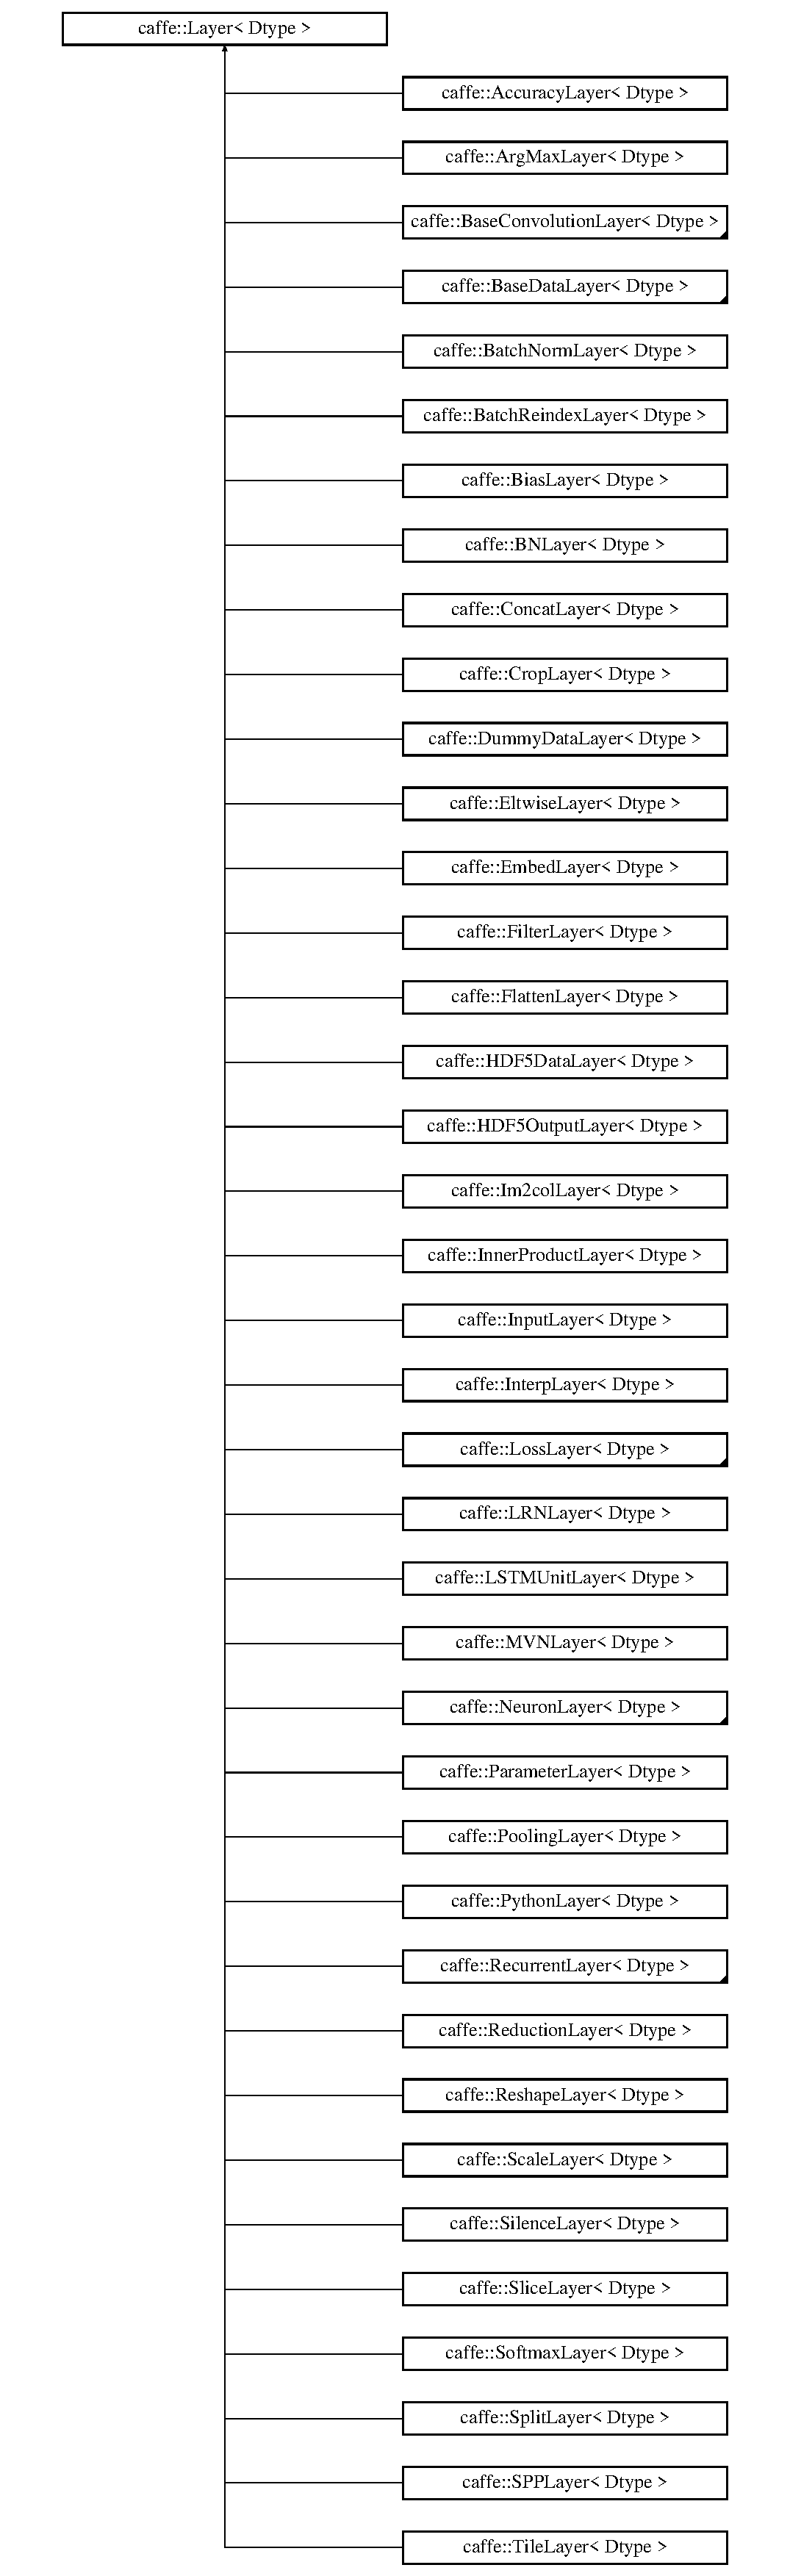
\includegraphics[height=12.000000cm]{classcaffe_1_1Layer}
\end{center}
\end{figure}
\subsection*{Public Member Functions}
\begin{DoxyCompactItemize}
\item 
\hyperlink{classcaffe_1_1Layer_a7b4e4ccea08c7b8b15acc6829d5735f6}{Layer} (const Layer\+Parameter \&param)
\item 
void \hyperlink{classcaffe_1_1Layer_ac427a267f4c5ba93caac53b7ba64841d}{Set\+Up} (const vector$<$ \hyperlink{classcaffe_1_1Blob}{Blob}$<$ Dtype $>$ $\ast$ $>$ \&bottom, const vector$<$ \hyperlink{classcaffe_1_1Blob}{Blob}$<$ Dtype $>$ $\ast$ $>$ \&top)
\begin{DoxyCompactList}\small\item\em Implements common layer setup functionality. \end{DoxyCompactList}\item 
virtual void \hyperlink{classcaffe_1_1Layer_a38dc2488bf319b8de5a7ac84e0045393}{Layer\+Set\+Up} (const vector$<$ \hyperlink{classcaffe_1_1Blob}{Blob}$<$ Dtype $>$ $\ast$ $>$ \&bottom, const vector$<$ \hyperlink{classcaffe_1_1Blob}{Blob}$<$ Dtype $>$ $\ast$ $>$ \&top)
\begin{DoxyCompactList}\small\item\em Does layer-\/specific setup\+: your layer should implement this function as well as Reshape. \end{DoxyCompactList}\item 
virtual void \hyperlink{classcaffe_1_1Layer_ad9d391b972c769c0ebee34ca6d1c973e}{Reshape} (const vector$<$ \hyperlink{classcaffe_1_1Blob}{Blob}$<$ Dtype $>$ $\ast$ $>$ \&bottom, const vector$<$ \hyperlink{classcaffe_1_1Blob}{Blob}$<$ Dtype $>$ $\ast$ $>$ \&top)=0
\begin{DoxyCompactList}\small\item\em Adjust the shapes of top blobs and internal buffers to accommodate the shapes of the bottom blobs. \end{DoxyCompactList}\item 
Dtype \hyperlink{classcaffe_1_1Layer_aa5fc9ddb31b58958653372bdaaccde94}{Forward} (const vector$<$ \hyperlink{classcaffe_1_1Blob}{Blob}$<$ Dtype $>$ $\ast$ $>$ \&bottom, const vector$<$ \hyperlink{classcaffe_1_1Blob}{Blob}$<$ Dtype $>$ $\ast$ $>$ \&top)
\begin{DoxyCompactList}\small\item\em Given the bottom blobs, compute the top blobs and the loss. \end{DoxyCompactList}\item 
void \hyperlink{classcaffe_1_1Layer_a53df1e081767e07bfb4c81657f4acd0a}{Backward} (const vector$<$ \hyperlink{classcaffe_1_1Blob}{Blob}$<$ Dtype $>$ $\ast$ $>$ \&top, const vector$<$ bool $>$ \&propagate\+\_\+down, const vector$<$ \hyperlink{classcaffe_1_1Blob}{Blob}$<$ Dtype $>$ $\ast$ $>$ \&bottom)
\begin{DoxyCompactList}\small\item\em Given the top blob error gradients, compute the bottom blob error gradients. \end{DoxyCompactList}\item 
vector$<$ shared\+\_\+ptr$<$ \hyperlink{classcaffe_1_1Blob}{Blob}$<$ Dtype $>$ $>$ $>$ \& \hyperlink{classcaffe_1_1Layer_aaf4524ce8641a30a8a4784aee1b2b4c8}{blobs} ()\hypertarget{classcaffe_1_1Layer_aaf4524ce8641a30a8a4784aee1b2b4c8}{}\label{classcaffe_1_1Layer_aaf4524ce8641a30a8a4784aee1b2b4c8}

\begin{DoxyCompactList}\small\item\em Returns the vector of learnable parameter blobs. \end{DoxyCompactList}\item 
const Layer\+Parameter \& \hyperlink{classcaffe_1_1Layer_af475062fe280614b18f642c4ccf50b40}{layer\+\_\+param} () const \hypertarget{classcaffe_1_1Layer_af475062fe280614b18f642c4ccf50b40}{}\label{classcaffe_1_1Layer_af475062fe280614b18f642c4ccf50b40}

\begin{DoxyCompactList}\small\item\em Returns the layer parameter. \end{DoxyCompactList}\item 
virtual void \hyperlink{classcaffe_1_1Layer_a4a1754828dda22cc8daa2f63377f3579}{To\+Proto} (Layer\+Parameter $\ast$param, bool write\+\_\+diff=false)\hypertarget{classcaffe_1_1Layer_a4a1754828dda22cc8daa2f63377f3579}{}\label{classcaffe_1_1Layer_a4a1754828dda22cc8daa2f63377f3579}

\begin{DoxyCompactList}\small\item\em Writes the layer parameter to a protocol buffer. \end{DoxyCompactList}\item 
Dtype \hyperlink{classcaffe_1_1Layer_a964ccba33b9a4b69391a72508f764eaf}{loss} (const int top\+\_\+index) const \hypertarget{classcaffe_1_1Layer_a964ccba33b9a4b69391a72508f764eaf}{}\label{classcaffe_1_1Layer_a964ccba33b9a4b69391a72508f764eaf}

\begin{DoxyCompactList}\small\item\em Returns the scalar loss associated with a top blob at a given index. \end{DoxyCompactList}\item 
void \hyperlink{classcaffe_1_1Layer_a899b09f4b91ada8545b3a43ee91e0d69}{set\+\_\+loss} (const int top\+\_\+index, const Dtype value)\hypertarget{classcaffe_1_1Layer_a899b09f4b91ada8545b3a43ee91e0d69}{}\label{classcaffe_1_1Layer_a899b09f4b91ada8545b3a43ee91e0d69}

\begin{DoxyCompactList}\small\item\em Sets the loss associated with a top blob at a given index. \end{DoxyCompactList}\item 
virtual const char $\ast$ \hyperlink{classcaffe_1_1Layer_a8c5deb0263ae572036c564d53902a08d}{type} () const \hypertarget{classcaffe_1_1Layer_a8c5deb0263ae572036c564d53902a08d}{}\label{classcaffe_1_1Layer_a8c5deb0263ae572036c564d53902a08d}

\begin{DoxyCompactList}\small\item\em Returns the layer type. \end{DoxyCompactList}\item 
virtual int \hyperlink{classcaffe_1_1Layer_a45c7a7943a8a6735ac433c9be11e0240}{Exact\+Num\+Bottom\+Blobs} () const 
\begin{DoxyCompactList}\small\item\em Returns the exact number of bottom blobs required by the layer, or -\/1 if no exact number is required. \end{DoxyCompactList}\item 
virtual int \hyperlink{classcaffe_1_1Layer_ade3eee97cc743c4e68fff7eba6484916}{Min\+Bottom\+Blobs} () const 
\begin{DoxyCompactList}\small\item\em Returns the minimum number of bottom blobs required by the layer, or -\/1 if no minimum number is required. \end{DoxyCompactList}\item 
virtual int \hyperlink{classcaffe_1_1Layer_a6408ef3939f1abed1abcec46ff219289}{Max\+Bottom\+Blobs} () const 
\begin{DoxyCompactList}\small\item\em Returns the maximum number of bottom blobs required by the layer, or -\/1 if no maximum number is required. \end{DoxyCompactList}\item 
virtual int \hyperlink{classcaffe_1_1Layer_aa3c99ed707e8db683a3043412e151af8}{Exact\+Num\+Top\+Blobs} () const 
\begin{DoxyCompactList}\small\item\em Returns the exact number of top blobs required by the layer, or -\/1 if no exact number is required. \end{DoxyCompactList}\item 
virtual int \hyperlink{classcaffe_1_1Layer_a8bb143d58a740345fa2dc3d4204d553b}{Min\+Top\+Blobs} () const 
\begin{DoxyCompactList}\small\item\em Returns the minimum number of top blobs required by the layer, or -\/1 if no minimum number is required. \end{DoxyCompactList}\item 
virtual int \hyperlink{classcaffe_1_1Layer_adeff774663c6ec94424901d2746e2f03}{Max\+Top\+Blobs} () const 
\begin{DoxyCompactList}\small\item\em Returns the maximum number of top blobs required by the layer, or -\/1 if no maximum number is required. \end{DoxyCompactList}\item 
virtual bool \hyperlink{classcaffe_1_1Layer_ad412187a0483c310bd59fd5f957faf0d}{Equal\+Num\+Bottom\+Top\+Blobs} () const 
\begin{DoxyCompactList}\small\item\em Returns true if the layer requires an equal number of bottom and top blobs. \end{DoxyCompactList}\item 
virtual bool \hyperlink{classcaffe_1_1Layer_ad732ca94cb21b4c4e0d6372a530ededf}{Auto\+Top\+Blobs} () const 
\begin{DoxyCompactList}\small\item\em Return whether \char`\"{}anonymous\char`\"{} top blobs are created automatically by the layer. \end{DoxyCompactList}\item 
virtual bool \hyperlink{classcaffe_1_1Layer_a4a2e4ca94eaa1cbc054b512c6657743e}{Allow\+Force\+Backward} (const int bottom\+\_\+index) const 
\begin{DoxyCompactList}\small\item\em Return whether to allow force\+\_\+backward for a given bottom blob index. \end{DoxyCompactList}\item 
bool \hyperlink{classcaffe_1_1Layer_a1a3708013b0231e71d725252e10ce6e3}{param\+\_\+propagate\+\_\+down} (const int param\+\_\+id)
\begin{DoxyCompactList}\small\item\em Specifies whether the layer should compute gradients w.\+r.\+t. a parameter at a particular index given by param\+\_\+id. \end{DoxyCompactList}\item 
void \hyperlink{classcaffe_1_1Layer_a9a6fcb843803ed556f0a69cc2864379b}{set\+\_\+param\+\_\+propagate\+\_\+down} (const int param\+\_\+id, const bool value)\hypertarget{classcaffe_1_1Layer_a9a6fcb843803ed556f0a69cc2864379b}{}\label{classcaffe_1_1Layer_a9a6fcb843803ed556f0a69cc2864379b}

\begin{DoxyCompactList}\small\item\em Sets whether the layer should compute gradients w.\+r.\+t. a parameter at a particular index given by param\+\_\+id. \end{DoxyCompactList}\end{DoxyCompactItemize}
\subsection*{Protected Member Functions}
\begin{DoxyCompactItemize}
\item 
virtual void \hyperlink{classcaffe_1_1Layer_add965883f75bbf90c7a06f960cda7a1a}{Forward\+\_\+cpu} (const vector$<$ \hyperlink{classcaffe_1_1Blob}{Blob}$<$ Dtype $>$ $\ast$ $>$ \&bottom, const vector$<$ \hyperlink{classcaffe_1_1Blob}{Blob}$<$ Dtype $>$ $\ast$ $>$ \&top)=0\hypertarget{classcaffe_1_1Layer_add965883f75bbf90c7a06f960cda7a1a}{}\label{classcaffe_1_1Layer_add965883f75bbf90c7a06f960cda7a1a}

\begin{DoxyCompactList}\small\item\em Using the C\+PU device, compute the layer output. \end{DoxyCompactList}\item 
virtual void \hyperlink{classcaffe_1_1Layer_a93b8d8c30c7691a39f634bf7bb2b03fb}{Forward\+\_\+gpu} (const vector$<$ \hyperlink{classcaffe_1_1Blob}{Blob}$<$ Dtype $>$ $\ast$ $>$ \&bottom, const vector$<$ \hyperlink{classcaffe_1_1Blob}{Blob}$<$ Dtype $>$ $\ast$ $>$ \&top)\hypertarget{classcaffe_1_1Layer_a93b8d8c30c7691a39f634bf7bb2b03fb}{}\label{classcaffe_1_1Layer_a93b8d8c30c7691a39f634bf7bb2b03fb}

\begin{DoxyCompactList}\small\item\em Using the G\+PU device, compute the layer output. Fall back to \hyperlink{classcaffe_1_1Layer_add965883f75bbf90c7a06f960cda7a1a}{Forward\+\_\+cpu()} if unavailable. \end{DoxyCompactList}\item 
virtual void \hyperlink{classcaffe_1_1Layer_a64d15855f882af4b82e83fa993c4e7c6}{Backward\+\_\+cpu} (const vector$<$ \hyperlink{classcaffe_1_1Blob}{Blob}$<$ Dtype $>$ $\ast$ $>$ \&top, const vector$<$ bool $>$ \&propagate\+\_\+down, const vector$<$ \hyperlink{classcaffe_1_1Blob}{Blob}$<$ Dtype $>$ $\ast$ $>$ \&bottom)=0\hypertarget{classcaffe_1_1Layer_a64d15855f882af4b82e83fa993c4e7c6}{}\label{classcaffe_1_1Layer_a64d15855f882af4b82e83fa993c4e7c6}

\begin{DoxyCompactList}\small\item\em Using the C\+PU device, compute the gradients for any parameters and for the bottom blobs if propagate\+\_\+down is true. \end{DoxyCompactList}\item 
virtual void \hyperlink{classcaffe_1_1Layer_a9275e5b8196feac9cf22803973c890f9}{Backward\+\_\+gpu} (const vector$<$ \hyperlink{classcaffe_1_1Blob}{Blob}$<$ Dtype $>$ $\ast$ $>$ \&top, const vector$<$ bool $>$ \&propagate\+\_\+down, const vector$<$ \hyperlink{classcaffe_1_1Blob}{Blob}$<$ Dtype $>$ $\ast$ $>$ \&bottom)\hypertarget{classcaffe_1_1Layer_a9275e5b8196feac9cf22803973c890f9}{}\label{classcaffe_1_1Layer_a9275e5b8196feac9cf22803973c890f9}

\begin{DoxyCompactList}\small\item\em Using the G\+PU device, compute the gradients for any parameters and for the bottom blobs if propagate\+\_\+down is true. Fall back to \hyperlink{classcaffe_1_1Layer_a64d15855f882af4b82e83fa993c4e7c6}{Backward\+\_\+cpu()} if unavailable. \end{DoxyCompactList}\item 
virtual void \hyperlink{classcaffe_1_1Layer_adaa95e30dff155409a25ffcb5c8c885e}{Check\+Blob\+Counts} (const vector$<$ \hyperlink{classcaffe_1_1Blob}{Blob}$<$ Dtype $>$ $\ast$ $>$ \&bottom, const vector$<$ \hyperlink{classcaffe_1_1Blob}{Blob}$<$ Dtype $>$ $\ast$ $>$ \&top)
\item 
void \hyperlink{classcaffe_1_1Layer_a8bd62d1505dd35d6a3a25954ae9e6014}{Set\+Loss\+Weights} (const vector$<$ \hyperlink{classcaffe_1_1Blob}{Blob}$<$ Dtype $>$ $\ast$ $>$ \&top)
\end{DoxyCompactItemize}
\subsection*{Protected Attributes}
\begin{DoxyCompactItemize}
\item 
Layer\+Parameter \hyperlink{classcaffe_1_1Layer_a7ed12bb2df25c887e41d7ea9557fc701}{layer\+\_\+param\+\_\+}
\item 
Phase \hyperlink{classcaffe_1_1Layer_a1d04ad7f595a82a1c811f102d68b8a19}{phase\+\_\+}
\item 
vector$<$ shared\+\_\+ptr$<$ \hyperlink{classcaffe_1_1Blob}{Blob}$<$ Dtype $>$ $>$ $>$ \hyperlink{classcaffe_1_1Layer_a8073fcf2c139b47eb99ce71b346b1321}{blobs\+\_\+}
\item 
vector$<$ bool $>$ \hyperlink{classcaffe_1_1Layer_acd4a05def9ff3b42ad72404210613ef7}{param\+\_\+propagate\+\_\+down\+\_\+}
\item 
vector$<$ Dtype $>$ \hyperlink{classcaffe_1_1Layer_af6d347229a139500994e7a926c680486}{loss\+\_\+}
\end{DoxyCompactItemize}


\subsection{Detailed Description}
\subsubsection*{template$<$typename Dtype$>$\\*
class caffe\+::\+Layer$<$ Dtype $>$}

An interface for the units of computation which can be composed into a \hyperlink{classcaffe_1_1Net}{Net}. 

\hyperlink{classcaffe_1_1Layer}{Layer}s must implement a Forward function, in which they take their input (bottom) \hyperlink{classcaffe_1_1Blob}{Blob}s (if any) and compute their output \hyperlink{classcaffe_1_1Blob}{Blob}s (if any). They may also implement a Backward function, in which they compute the error gradients with respect to their input \hyperlink{classcaffe_1_1Blob}{Blob}s, given the error gradients with their output \hyperlink{classcaffe_1_1Blob}{Blob}s. 

\subsection{Constructor \& Destructor Documentation}
\index{caffe\+::\+Layer@{caffe\+::\+Layer}!Layer@{Layer}}
\index{Layer@{Layer}!caffe\+::\+Layer@{caffe\+::\+Layer}}
\subsubsection[{\texorpdfstring{Layer(const Layer\+Parameter \&param)}{Layer(const LayerParameter &param)}}]{\setlength{\rightskip}{0pt plus 5cm}template$<$typename Dtype $>$ {\bf caffe\+::\+Layer}$<$ Dtype $>$\+::{\bf Layer} (
\begin{DoxyParamCaption}
\item[{const Layer\+Parameter \&}]{param}
\end{DoxyParamCaption}
)\hspace{0.3cm}{\ttfamily [inline]}, {\ttfamily [explicit]}}\hypertarget{classcaffe_1_1Layer_a7b4e4ccea08c7b8b15acc6829d5735f6}{}\label{classcaffe_1_1Layer_a7b4e4ccea08c7b8b15acc6829d5735f6}
You should not implement your own constructor. Any set up code should go to \hyperlink{classcaffe_1_1Layer_ac427a267f4c5ba93caac53b7ba64841d}{Set\+Up()}, where the dimensions of the bottom blobs are provided to the layer. 

\subsection{Member Function Documentation}
\index{caffe\+::\+Layer@{caffe\+::\+Layer}!Allow\+Force\+Backward@{Allow\+Force\+Backward}}
\index{Allow\+Force\+Backward@{Allow\+Force\+Backward}!caffe\+::\+Layer@{caffe\+::\+Layer}}
\subsubsection[{\texorpdfstring{Allow\+Force\+Backward(const int bottom\+\_\+index) const }{AllowForceBackward(const int bottom_index) const }}]{\setlength{\rightskip}{0pt plus 5cm}template$<$typename Dtype $>$ virtual bool {\bf caffe\+::\+Layer}$<$ Dtype $>$\+::Allow\+Force\+Backward (
\begin{DoxyParamCaption}
\item[{const int}]{bottom\+\_\+index}
\end{DoxyParamCaption}
) const\hspace{0.3cm}{\ttfamily [inline]}, {\ttfamily [virtual]}}\hypertarget{classcaffe_1_1Layer_a4a2e4ca94eaa1cbc054b512c6657743e}{}\label{classcaffe_1_1Layer_a4a2e4ca94eaa1cbc054b512c6657743e}


Return whether to allow force\+\_\+backward for a given bottom blob index. 

If Allow\+Force\+Backward(i) == false, we will ignore the force\+\_\+backward setting and backpropagate to blob i only if it needs gradient information (as is done when force\+\_\+backward == false). 

Reimplemented in \hyperlink{classcaffe_1_1LSTMUnitLayer_a28bbfffaf2a438f151566c7e53bbc1d7}{caffe\+::\+L\+S\+T\+M\+Unit\+Layer$<$ Dtype $>$}, \hyperlink{classcaffe_1_1RecurrentLayer_ac8642c8d7f418b6513c93daffa5eb15e}{caffe\+::\+Recurrent\+Layer$<$ Dtype $>$}, \hyperlink{classcaffe_1_1EuclideanLossLayer_a3c954fd7c15596fd2f59e0f79601905c}{caffe\+::\+Euclidean\+Loss\+Layer$<$ Dtype $>$}, \hyperlink{classcaffe_1_1ContrastiveLossLayer_afbfe9d1707c9e76e31fe381af3d708ef}{caffe\+::\+Contrastive\+Loss\+Layer$<$ Dtype $>$}, and \hyperlink{classcaffe_1_1LossLayer_ad02fe695b06451ac8e6f21db0cba1dad}{caffe\+::\+Loss\+Layer$<$ Dtype $>$}.

\index{caffe\+::\+Layer@{caffe\+::\+Layer}!Auto\+Top\+Blobs@{Auto\+Top\+Blobs}}
\index{Auto\+Top\+Blobs@{Auto\+Top\+Blobs}!caffe\+::\+Layer@{caffe\+::\+Layer}}
\subsubsection[{\texorpdfstring{Auto\+Top\+Blobs() const }{AutoTopBlobs() const }}]{\setlength{\rightskip}{0pt plus 5cm}template$<$typename Dtype $>$ virtual bool {\bf caffe\+::\+Layer}$<$ Dtype $>$\+::Auto\+Top\+Blobs (
\begin{DoxyParamCaption}
{}
\end{DoxyParamCaption}
) const\hspace{0.3cm}{\ttfamily [inline]}, {\ttfamily [virtual]}}\hypertarget{classcaffe_1_1Layer_ad732ca94cb21b4c4e0d6372a530ededf}{}\label{classcaffe_1_1Layer_ad732ca94cb21b4c4e0d6372a530ededf}


Return whether \char`\"{}anonymous\char`\"{} top blobs are created automatically by the layer. 

If this method returns true, \hyperlink{classcaffe_1_1Net_ae9fcfaabc89165d6c0cb4b14b4c6b584}{Net\+::\+Init} will create enough \char`\"{}anonymous\char`\"{} top blobs to fulfill the requirement specified by \hyperlink{classcaffe_1_1Layer_aa3c99ed707e8db683a3043412e151af8}{Exact\+Num\+Top\+Blobs()} or \hyperlink{classcaffe_1_1Layer_a8bb143d58a740345fa2dc3d4204d553b}{Min\+Top\+Blobs()}. 

Reimplemented in \hyperlink{classcaffe_1_1LossLayer_ad272e6792a781ce4f66a65057cc829d1}{caffe\+::\+Loss\+Layer$<$ Dtype $>$}.

\index{caffe\+::\+Layer@{caffe\+::\+Layer}!Backward@{Backward}}
\index{Backward@{Backward}!caffe\+::\+Layer@{caffe\+::\+Layer}}
\subsubsection[{\texorpdfstring{Backward(const vector$<$ Blob$<$ Dtype $>$ $\ast$ $>$ \&top, const vector$<$ bool $>$ \&propagate\+\_\+down, const vector$<$ Blob$<$ Dtype $>$ $\ast$ $>$ \&bottom)}{Backward(const vector< Blob< Dtype > * > &top, const vector< bool > &propagate_down, const vector< Blob< Dtype > * > &bottom)}}]{\setlength{\rightskip}{0pt plus 5cm}template$<$typename Dtype $>$ void {\bf caffe\+::\+Layer}$<$ Dtype $>$\+::Backward (
\begin{DoxyParamCaption}
\item[{const vector$<$ {\bf Blob}$<$ Dtype $>$ $\ast$ $>$ \&}]{top, }
\item[{const vector$<$ bool $>$ \&}]{propagate\+\_\+down, }
\item[{const vector$<$ {\bf Blob}$<$ Dtype $>$ $\ast$ $>$ \&}]{bottom}
\end{DoxyParamCaption}
)\hspace{0.3cm}{\ttfamily [inline]}}\hypertarget{classcaffe_1_1Layer_a53df1e081767e07bfb4c81657f4acd0a}{}\label{classcaffe_1_1Layer_a53df1e081767e07bfb4c81657f4acd0a}


Given the top blob error gradients, compute the bottom blob error gradients. 


\begin{DoxyParams}{Parameters}
{\em top} & the output blobs, whose diff fields store the gradient of the error with respect to themselves \\
\hline
{\em propagate\+\_\+down} & a vector with equal length to bottom, with each index indicating whether to propagate the error gradients down to the bottom blob at the corresponding index \\
\hline
{\em bottom} & the input blobs, whose diff fields will store the gradient of the error with respect to themselves after Backward is run\\
\hline
\end{DoxyParams}
The Backward wrapper calls the relevant device wrapper function (Backward\+\_\+cpu or Backward\+\_\+gpu) to compute the bottom blob diffs given the top blob diffs.

Your layer should implement Backward\+\_\+cpu and (optionally) Backward\+\_\+gpu. \index{caffe\+::\+Layer@{caffe\+::\+Layer}!Check\+Blob\+Counts@{Check\+Blob\+Counts}}
\index{Check\+Blob\+Counts@{Check\+Blob\+Counts}!caffe\+::\+Layer@{caffe\+::\+Layer}}
\subsubsection[{\texorpdfstring{Check\+Blob\+Counts(const vector$<$ Blob$<$ Dtype $>$ $\ast$ $>$ \&bottom, const vector$<$ Blob$<$ Dtype $>$ $\ast$ $>$ \&top)}{CheckBlobCounts(const vector< Blob< Dtype > * > &bottom, const vector< Blob< Dtype > * > &top)}}]{\setlength{\rightskip}{0pt plus 5cm}template$<$typename Dtype $>$ virtual void {\bf caffe\+::\+Layer}$<$ Dtype $>$\+::Check\+Blob\+Counts (
\begin{DoxyParamCaption}
\item[{const vector$<$ {\bf Blob}$<$ Dtype $>$ $\ast$ $>$ \&}]{bottom, }
\item[{const vector$<$ {\bf Blob}$<$ Dtype $>$ $\ast$ $>$ \&}]{top}
\end{DoxyParamCaption}
)\hspace{0.3cm}{\ttfamily [inline]}, {\ttfamily [protected]}, {\ttfamily [virtual]}}\hypertarget{classcaffe_1_1Layer_adaa95e30dff155409a25ffcb5c8c885e}{}\label{classcaffe_1_1Layer_adaa95e30dff155409a25ffcb5c8c885e}
Called by the parent \hyperlink{classcaffe_1_1Layer}{Layer}\textquotesingle{}s Set\+Up to check that the number of bottom and top Blobs provided as input match the expected numbers specified by the \{Exact\+Num,Min,Max\}\{Bottom,Top\}Blobs() functions. \index{caffe\+::\+Layer@{caffe\+::\+Layer}!Equal\+Num\+Bottom\+Top\+Blobs@{Equal\+Num\+Bottom\+Top\+Blobs}}
\index{Equal\+Num\+Bottom\+Top\+Blobs@{Equal\+Num\+Bottom\+Top\+Blobs}!caffe\+::\+Layer@{caffe\+::\+Layer}}
\subsubsection[{\texorpdfstring{Equal\+Num\+Bottom\+Top\+Blobs() const }{EqualNumBottomTopBlobs() const }}]{\setlength{\rightskip}{0pt plus 5cm}template$<$typename Dtype $>$ virtual bool {\bf caffe\+::\+Layer}$<$ Dtype $>$\+::Equal\+Num\+Bottom\+Top\+Blobs (
\begin{DoxyParamCaption}
{}
\end{DoxyParamCaption}
) const\hspace{0.3cm}{\ttfamily [inline]}, {\ttfamily [virtual]}}\hypertarget{classcaffe_1_1Layer_ad412187a0483c310bd59fd5f957faf0d}{}\label{classcaffe_1_1Layer_ad412187a0483c310bd59fd5f957faf0d}


Returns true if the layer requires an equal number of bottom and top blobs. 

This method should be overridden to return true if your layer expects an equal number of bottom and top blobs. 

Reimplemented in \hyperlink{classcaffe_1_1BaseConvolutionLayer_add4567680b9466cbae5804da6a76e2ee}{caffe\+::\+Base\+Convolution\+Layer$<$ Dtype $>$}.

\index{caffe\+::\+Layer@{caffe\+::\+Layer}!Exact\+Num\+Bottom\+Blobs@{Exact\+Num\+Bottom\+Blobs}}
\index{Exact\+Num\+Bottom\+Blobs@{Exact\+Num\+Bottom\+Blobs}!caffe\+::\+Layer@{caffe\+::\+Layer}}
\subsubsection[{\texorpdfstring{Exact\+Num\+Bottom\+Blobs() const }{ExactNumBottomBlobs() const }}]{\setlength{\rightskip}{0pt plus 5cm}template$<$typename Dtype $>$ virtual int {\bf caffe\+::\+Layer}$<$ Dtype $>$\+::Exact\+Num\+Bottom\+Blobs (
\begin{DoxyParamCaption}
{}
\end{DoxyParamCaption}
) const\hspace{0.3cm}{\ttfamily [inline]}, {\ttfamily [virtual]}}\hypertarget{classcaffe_1_1Layer_a45c7a7943a8a6735ac433c9be11e0240}{}\label{classcaffe_1_1Layer_a45c7a7943a8a6735ac433c9be11e0240}


Returns the exact number of bottom blobs required by the layer, or -\/1 if no exact number is required. 

This method should be overridden to return a non-\/negative value if your layer expects some exact number of bottom blobs. 

Reimplemented in \hyperlink{classcaffe_1_1LSTMUnitLayer_a865a9e9d8b1d24cd46cabcec81169b01}{caffe\+::\+L\+S\+T\+M\+Unit\+Layer$<$ Dtype $>$}, \hyperlink{classcaffe_1_1InfogainLossLayer_aef9aa9200a3129d7bddf56f717017cbb}{caffe\+::\+Infogain\+Loss\+Layer$<$ Dtype $>$}, \hyperlink{classcaffe_1_1BatchNormLayer_a30b42ad6c976170fc0a8c523682ff96a}{caffe\+::\+Batch\+Norm\+Layer$<$ Dtype $>$}, \hyperlink{classcaffe_1_1ArgMaxLayer_ab9acebe420760d367c6e5808842411d0}{caffe\+::\+Arg\+Max\+Layer$<$ Dtype $>$}, \hyperlink{classcaffe_1_1ContrastiveLossLayer_af1b8bcaf8ddacd3e98e26c558c7f49a0}{caffe\+::\+Contrastive\+Loss\+Layer$<$ Dtype $>$}, \hyperlink{classcaffe_1_1AccuracyLayer_afcde815835ab4cdf76fbbef610491a91}{caffe\+::\+Accuracy\+Layer$<$ Dtype $>$}, \hyperlink{classcaffe_1_1HDF5OutputLayer_af874ff0bf8f1817f44d18398889bcbe4}{caffe\+::\+H\+D\+F5\+Output\+Layer$<$ Dtype $>$}, \hyperlink{classcaffe_1_1HDF5DataLayer_a800a76c3afa9d5ac8042fa08d01b3bef}{caffe\+::\+H\+D\+F5\+Data\+Layer$<$ Dtype $>$}, \hyperlink{classcaffe_1_1WindowDataLayer_ac6c818494dd8d3636523556c858908c4}{caffe\+::\+Window\+Data\+Layer$<$ Dtype $>$}, \hyperlink{classcaffe_1_1AbsValLayer_a0e797616508e76aa9c2ce19a1b08dff0}{caffe\+::\+Abs\+Val\+Layer$<$ Dtype $>$}, \hyperlink{classcaffe_1_1LRNLayer_aabbbcdeb646c188ac2137b003aa1c682}{caffe\+::\+L\+R\+N\+Layer$<$ Dtype $>$}, \hyperlink{classcaffe_1_1ImageDataLayer_a95155f868560cf481138deb7a999ee08}{caffe\+::\+Image\+Data\+Layer$<$ Dtype $>$}, \hyperlink{classcaffe_1_1LossLayer_a8a2e16d4691640c34e589aac4ec42e28}{caffe\+::\+Loss\+Layer$<$ Dtype $>$}, \hyperlink{classcaffe_1_1CropLayer_a1c74edc80c22d805a96b00fefceb3286}{caffe\+::\+Crop\+Layer$<$ Dtype $>$}, \hyperlink{classcaffe_1_1FlattenLayer_ad7abb8ccc06c7943e79d77bf5a7e2521}{caffe\+::\+Flatten\+Layer$<$ Dtype $>$}, \hyperlink{classcaffe_1_1DummyDataLayer_ad25325d52be96802665c21acc792c6dc}{caffe\+::\+Dummy\+Data\+Layer$<$ Dtype $>$}, \hyperlink{classcaffe_1_1EmbedLayer_ad32929e7b7b9f3467425065c1d037c07}{caffe\+::\+Embed\+Layer$<$ Dtype $>$}, \hyperlink{classcaffe_1_1Im2colLayer_aba3720be3f1f71f9e44fbfba90ae3ac0}{caffe\+::\+Im2col\+Layer$<$ Dtype $>$}, \hyperlink{classcaffe_1_1InputLayer_a5bb058da95fd98a74385bbd3eccbe56b}{caffe\+::\+Input\+Layer$<$ Dtype $>$}, \hyperlink{classcaffe_1_1ReductionLayer_ae867c60a3ff94496f9a375b606c00bd3}{caffe\+::\+Reduction\+Layer$<$ Dtype $>$}, \hyperlink{classcaffe_1_1BatchReindexLayer_ab84d37975127bfe16593c082731c6f55}{caffe\+::\+Batch\+Reindex\+Layer$<$ Dtype $>$}, \hyperlink{classcaffe_1_1InnerProductLayer_a53daee4cea7f8902042418a3925ee0a5}{caffe\+::\+Inner\+Product\+Layer$<$ Dtype $>$}, \hyperlink{classcaffe_1_1ParameterLayer_ae1150a72fa6add67511d92da2cb8216a}{caffe\+::\+Parameter\+Layer$<$ Dtype $>$}, \hyperlink{classcaffe_1_1ReshapeLayer_adf4f419172a77dbef9535dcd9f69f8c6}{caffe\+::\+Reshape\+Layer$<$ Dtype $>$}, \hyperlink{classcaffe_1_1SliceLayer_a7f140bb3775c60a2d3d60298802d2b85}{caffe\+::\+Slice\+Layer$<$ Dtype $>$}, \hyperlink{classcaffe_1_1SPPLayer_ab6912cfa8daa151407d024d5113e10b0}{caffe\+::\+S\+P\+P\+Layer$<$ Dtype $>$}, \hyperlink{classcaffe_1_1BNLayer_a534fd38c3c24115d5c5676362816157b}{caffe\+::\+B\+N\+Layer$<$ Dtype $>$}, \hyperlink{classcaffe_1_1InterpLayer_a186c0c177d96da2dce60308d78959c2b}{caffe\+::\+Interp\+Layer$<$ Dtype $>$}, \hyperlink{classcaffe_1_1MemoryDataLayer_a46529bcce2bf8b8f3984286ad675cbd6}{caffe\+::\+Memory\+Data\+Layer$<$ Dtype $>$}, \hyperlink{classcaffe_1_1PoolingLayer_a6fc8f79729e17639d3b97781791e352d}{caffe\+::\+Pooling\+Layer$<$ Dtype $>$}, \hyperlink{classcaffe_1_1SplitLayer_abdf26784113e37451b5c9e4b5181badb}{caffe\+::\+Split\+Layer$<$ Dtype $>$}, \hyperlink{classcaffe_1_1MVNLayer_a5766f86a41a05a585dfceeb944b6ca2c}{caffe\+::\+M\+V\+N\+Layer$<$ Dtype $>$}, \hyperlink{classcaffe_1_1NeuronLayer_a83678ec7f661054d36d83fa062b639b2}{caffe\+::\+Neuron\+Layer$<$ Dtype $>$}, \hyperlink{classcaffe_1_1SoftmaxLayer_a6b8863006cf34812d01354b671406816}{caffe\+::\+Softmax\+Layer$<$ Dtype $>$}, \hyperlink{classcaffe_1_1DataLayer_a41c3c270f2f1239808fbd4293e89949d}{caffe\+::\+Data\+Layer$<$ Dtype $>$}, and \hyperlink{classcaffe_1_1TileLayer_a7135c09877493a4ac9533f3952af74ae}{caffe\+::\+Tile\+Layer$<$ Dtype $>$}.

\index{caffe\+::\+Layer@{caffe\+::\+Layer}!Exact\+Num\+Top\+Blobs@{Exact\+Num\+Top\+Blobs}}
\index{Exact\+Num\+Top\+Blobs@{Exact\+Num\+Top\+Blobs}!caffe\+::\+Layer@{caffe\+::\+Layer}}
\subsubsection[{\texorpdfstring{Exact\+Num\+Top\+Blobs() const }{ExactNumTopBlobs() const }}]{\setlength{\rightskip}{0pt plus 5cm}template$<$typename Dtype $>$ virtual int {\bf caffe\+::\+Layer}$<$ Dtype $>$\+::Exact\+Num\+Top\+Blobs (
\begin{DoxyParamCaption}
{}
\end{DoxyParamCaption}
) const\hspace{0.3cm}{\ttfamily [inline]}, {\ttfamily [virtual]}}\hypertarget{classcaffe_1_1Layer_aa3c99ed707e8db683a3043412e151af8}{}\label{classcaffe_1_1Layer_aa3c99ed707e8db683a3043412e151af8}


Returns the exact number of top blobs required by the layer, or -\/1 if no exact number is required. 

This method should be overridden to return a non-\/negative value if your layer expects some exact number of top blobs. 

Reimplemented in \hyperlink{classcaffe_1_1LSTMUnitLayer_a6e547d63245347dac2aa412281d93970}{caffe\+::\+L\+S\+T\+M\+Unit\+Layer$<$ Dtype $>$}, \hyperlink{classcaffe_1_1InfogainLossLayer_aa25f7b12805d10dccc217669f589fc95}{caffe\+::\+Infogain\+Loss\+Layer$<$ Dtype $>$}, \hyperlink{classcaffe_1_1SoftmaxWithLossLayer_a8222589f986db56372bf00935bae6180}{caffe\+::\+Softmax\+With\+Loss\+Layer$<$ Dtype $>$}, \hyperlink{classcaffe_1_1BatchNormLayer_ad9fb4bf90a79a0a739ed1223628a88b9}{caffe\+::\+Batch\+Norm\+Layer$<$ Dtype $>$}, \hyperlink{classcaffe_1_1ArgMaxLayer_acb86bae0a6dd2f01688ed4575830b874}{caffe\+::\+Arg\+Max\+Layer$<$ Dtype $>$}, \hyperlink{classcaffe_1_1RecurrentLayer_ac53fa5447232a9067ef30028ad9da1cc}{caffe\+::\+Recurrent\+Layer$<$ Dtype $>$}, \hyperlink{classcaffe_1_1LossLayer_af8dca16967e8e979ebead4e80664dc10}{caffe\+::\+Loss\+Layer$<$ Dtype $>$}, \hyperlink{classcaffe_1_1ScaleLayer_a41c1e942cff6005f71b882d0c5039cf0}{caffe\+::\+Scale\+Layer$<$ Dtype $>$}, \hyperlink{classcaffe_1_1HDF5OutputLayer_a2c754adb8c37b1299507865fdb616149}{caffe\+::\+H\+D\+F5\+Output\+Layer$<$ Dtype $>$}, \hyperlink{classcaffe_1_1WindowDataLayer_ae322bcc85f1d1ac2dc59e1ff28c29e7a}{caffe\+::\+Window\+Data\+Layer$<$ Dtype $>$}, \hyperlink{classcaffe_1_1AbsValLayer_abddadbf826dc2ffaf22738804a484208}{caffe\+::\+Abs\+Val\+Layer$<$ Dtype $>$}, \hyperlink{classcaffe_1_1BiasLayer_a62bf10551992b95ecd499f1ce50f9465}{caffe\+::\+Bias\+Layer$<$ Dtype $>$}, \hyperlink{classcaffe_1_1LRNLayer_aab9056708727154a01866d17756c07cc}{caffe\+::\+L\+R\+N\+Layer$<$ Dtype $>$}, \hyperlink{classcaffe_1_1ImageDataLayer_a288e0fe3bca4334100e077bc0ad20c60}{caffe\+::\+Image\+Data\+Layer$<$ Dtype $>$}, \hyperlink{classcaffe_1_1CropLayer_a3335d668f97fe9582e29a684922adc97}{caffe\+::\+Crop\+Layer$<$ Dtype $>$}, \hyperlink{classcaffe_1_1FlattenLayer_ab54601497218724036abfcec46a718de}{caffe\+::\+Flatten\+Layer$<$ Dtype $>$}, \hyperlink{classcaffe_1_1EmbedLayer_a4555e4767b2ce8a32a23e5b1281f8a91}{caffe\+::\+Embed\+Layer$<$ Dtype $>$}, \hyperlink{classcaffe_1_1Im2colLayer_aa4aa1cfc956fa1ab3656ad2adf911f32}{caffe\+::\+Im2col\+Layer$<$ Dtype $>$}, \hyperlink{classcaffe_1_1ReductionLayer_ada0483efdbad3a50f6fc8466cef482bd}{caffe\+::\+Reduction\+Layer$<$ Dtype $>$}, \hyperlink{classcaffe_1_1BatchReindexLayer_afc9d0ae372b83e2b9e82228893313dc3}{caffe\+::\+Batch\+Reindex\+Layer$<$ Dtype $>$}, \hyperlink{classcaffe_1_1EltwiseLayer_adab35a7e096edeb73670e6682f264774}{caffe\+::\+Eltwise\+Layer$<$ Dtype $>$}, \hyperlink{classcaffe_1_1InnerProductLayer_a14a316bbfecc839fc65dc9c8aadc0b6d}{caffe\+::\+Inner\+Product\+Layer$<$ Dtype $>$}, \hyperlink{classcaffe_1_1ParameterLayer_a7db6cdb07222be5b9eb462c0ac64b363}{caffe\+::\+Parameter\+Layer$<$ Dtype $>$}, \hyperlink{classcaffe_1_1ReshapeLayer_aa624eade2fa1947073070bfcfa08f374}{caffe\+::\+Reshape\+Layer$<$ Dtype $>$}, \hyperlink{classcaffe_1_1SPPLayer_a698395fdd26563b18ea0fac07d4e8026}{caffe\+::\+S\+P\+P\+Layer$<$ Dtype $>$}, \hyperlink{classcaffe_1_1BNLayer_a4d608d903ec320429ef155d90aaf9926}{caffe\+::\+B\+N\+Layer$<$ Dtype $>$}, \hyperlink{classcaffe_1_1InterpLayer_a14e1a12b196cd87eef112d7a87d5e75e}{caffe\+::\+Interp\+Layer$<$ Dtype $>$}, \hyperlink{classcaffe_1_1MemoryDataLayer_a973a58b5967809488f0e88c0a9a6fbac}{caffe\+::\+Memory\+Data\+Layer$<$ Dtype $>$}, \hyperlink{classcaffe_1_1ConcatLayer_a3ee6697895b9c39e60b0019eedd7af68}{caffe\+::\+Concat\+Layer$<$ Dtype $>$}, \hyperlink{classcaffe_1_1MVNLayer_a0c5e5f3645dcc3b9dc5886cee9e6f302}{caffe\+::\+M\+V\+N\+Layer$<$ Dtype $>$}, \hyperlink{classcaffe_1_1NeuronLayer_a25dfa84e8b46705aa7a822e734b4f04f}{caffe\+::\+Neuron\+Layer$<$ Dtype $>$}, \hyperlink{classcaffe_1_1SoftmaxLayer_ae5c54555352700247a8fe47b73d06ce7}{caffe\+::\+Softmax\+Layer$<$ Dtype $>$}, \hyperlink{classcaffe_1_1SilenceLayer_a9bea0b5a6e1c15eefc85fdcc58d1c2e7}{caffe\+::\+Silence\+Layer$<$ Dtype $>$}, and \hyperlink{classcaffe_1_1TileLayer_a4f442a78d1234169a1ef3d51f2eda9e4}{caffe\+::\+Tile\+Layer$<$ Dtype $>$}.

\index{caffe\+::\+Layer@{caffe\+::\+Layer}!Forward@{Forward}}
\index{Forward@{Forward}!caffe\+::\+Layer@{caffe\+::\+Layer}}
\subsubsection[{\texorpdfstring{Forward(const vector$<$ Blob$<$ Dtype $>$ $\ast$ $>$ \&bottom, const vector$<$ Blob$<$ Dtype $>$ $\ast$ $>$ \&top)}{Forward(const vector< Blob< Dtype > * > &bottom, const vector< Blob< Dtype > * > &top)}}]{\setlength{\rightskip}{0pt plus 5cm}template$<$typename Dtype $>$ Dtype {\bf caffe\+::\+Layer}$<$ Dtype $>$\+::Forward (
\begin{DoxyParamCaption}
\item[{const vector$<$ {\bf Blob}$<$ Dtype $>$ $\ast$ $>$ \&}]{bottom, }
\item[{const vector$<$ {\bf Blob}$<$ Dtype $>$ $\ast$ $>$ \&}]{top}
\end{DoxyParamCaption}
)\hspace{0.3cm}{\ttfamily [inline]}}\hypertarget{classcaffe_1_1Layer_aa5fc9ddb31b58958653372bdaaccde94}{}\label{classcaffe_1_1Layer_aa5fc9ddb31b58958653372bdaaccde94}


Given the bottom blobs, compute the top blobs and the loss. 


\begin{DoxyParams}{Parameters}
{\em bottom} & the input blobs, whose data fields store the input data for this layer \\
\hline
{\em top} & the preshaped output blobs, whose data fields will store this layers\textquotesingle{} outputs \\
\hline
\end{DoxyParams}
\begin{DoxyReturn}{Returns}
The total loss from the layer.
\end{DoxyReturn}
The Forward wrapper calls the relevant device wrapper function (Forward\+\_\+cpu or Forward\+\_\+gpu) to compute the top blob values given the bottom blobs. If the layer has any non-\/zero loss\+\_\+weights, the wrapper then computes and returns the loss.

Your layer should implement Forward\+\_\+cpu and (optionally) Forward\+\_\+gpu. \index{caffe\+::\+Layer@{caffe\+::\+Layer}!Layer\+Set\+Up@{Layer\+Set\+Up}}
\index{Layer\+Set\+Up@{Layer\+Set\+Up}!caffe\+::\+Layer@{caffe\+::\+Layer}}
\subsubsection[{\texorpdfstring{Layer\+Set\+Up(const vector$<$ Blob$<$ Dtype $>$ $\ast$ $>$ \&bottom, const vector$<$ Blob$<$ Dtype $>$ $\ast$ $>$ \&top)}{LayerSetUp(const vector< Blob< Dtype > * > &bottom, const vector< Blob< Dtype > * > &top)}}]{\setlength{\rightskip}{0pt plus 5cm}template$<$typename Dtype $>$ virtual void {\bf caffe\+::\+Layer}$<$ Dtype $>$\+::Layer\+Set\+Up (
\begin{DoxyParamCaption}
\item[{const vector$<$ {\bf Blob}$<$ Dtype $>$ $\ast$ $>$ \&}]{bottom, }
\item[{const vector$<$ {\bf Blob}$<$ Dtype $>$ $\ast$ $>$ \&}]{top}
\end{DoxyParamCaption}
)\hspace{0.3cm}{\ttfamily [inline]}, {\ttfamily [virtual]}}\hypertarget{classcaffe_1_1Layer_a38dc2488bf319b8de5a7ac84e0045393}{}\label{classcaffe_1_1Layer_a38dc2488bf319b8de5a7ac84e0045393}


Does layer-\/specific setup\+: your layer should implement this function as well as Reshape. 


\begin{DoxyParams}{Parameters}
{\em bottom} & the preshaped input blobs, whose data fields store the input data for this layer \\
\hline
{\em top} & the allocated but unshaped output blobs\\
\hline
\end{DoxyParams}
This method should do one-\/time layer specific setup. This includes reading and processing relevent parameters from the {\ttfamily layer\+\_\+param\+\_\+}. Setting up the shapes of top blobs and internal buffers should be done in {\ttfamily Reshape}, which will be called before the forward pass to adjust the top blob sizes. 

Reimplemented in \hyperlink{classcaffe_1_1BasePrefetchingDataLayer_af433228727bf4f3f3aaa85434efc93c5}{caffe\+::\+Base\+Prefetching\+Data\+Layer$<$ Dtype $>$}, \hyperlink{classcaffe_1_1SoftmaxWithLossLayer_a063c4e9786bc09f4773cb082c2960eb5}{caffe\+::\+Softmax\+With\+Loss\+Layer$<$ Dtype $>$}, \hyperlink{classcaffe_1_1InfogainLossLayer_a55a1d7ae2db81750c33ef9286764cd29}{caffe\+::\+Infogain\+Loss\+Layer$<$ Dtype $>$}, \hyperlink{classcaffe_1_1SigmoidCrossEntropyLossLayer_a87a48fa111fae84f238259d77263459e}{caffe\+::\+Sigmoid\+Cross\+Entropy\+Loss\+Layer$<$ Dtype $>$}, \hyperlink{classcaffe_1_1BatchNormLayer_ae4784dc3c124ea934b1d9736d465591f}{caffe\+::\+Batch\+Norm\+Layer$<$ Dtype $>$}, \hyperlink{classcaffe_1_1ContrastiveLossLayer_a34a16b3e6598ec6c23e63c01ef0c0a99}{caffe\+::\+Contrastive\+Loss\+Layer$<$ Dtype $>$}, \hyperlink{classcaffe_1_1ArgMaxLayer_a479814976e31716e670d63c126e5036f}{caffe\+::\+Arg\+Max\+Layer$<$ Dtype $>$}, \hyperlink{classcaffe_1_1DropoutLayer_a82bcd23115526808c79c807686945145}{caffe\+::\+Dropout\+Layer$<$ Dtype $>$}, \hyperlink{classcaffe_1_1PReLULayer_ad80124134d59ef7eff37601c953f09ef}{caffe\+::\+P\+Re\+L\+U\+Layer$<$ Dtype $>$}, \hyperlink{classcaffe_1_1SwishLayer_a07ce69f7855f0374ad826fb59fc58712}{caffe\+::\+Swish\+Layer$<$ Dtype $>$}, \hyperlink{classcaffe_1_1ExpLayer_a5f88102bf4922032eeab431154a76710}{caffe\+::\+Exp\+Layer$<$ Dtype $>$}, \hyperlink{classcaffe_1_1LogLayer_ab3f8854a38095f499e44ad8edf15b97b}{caffe\+::\+Log\+Layer$<$ Dtype $>$}, \hyperlink{classcaffe_1_1AccuracyLayer_aa4e6baa79f0c23308c39be3fe5085971}{caffe\+::\+Accuracy\+Layer$<$ Dtype $>$}, \hyperlink{classcaffe_1_1PowerLayer_aa8f097be5b0f8d7dd104e88dc2a2e544}{caffe\+::\+Power\+Layer$<$ Dtype $>$}, \hyperlink{classcaffe_1_1RecurrentLayer_aafa788d0a3535c80478fee74b9dbb62b}{caffe\+::\+Recurrent\+Layer$<$ Dtype $>$}, \hyperlink{classcaffe_1_1ScaleLayer_a04dae324b07eaee6775f9a972c9ab3ab}{caffe\+::\+Scale\+Layer$<$ Dtype $>$}, \hyperlink{classcaffe_1_1AbsValLayer_acfb0677a17e9d3b4920ff62d3b0d800a}{caffe\+::\+Abs\+Val\+Layer$<$ Dtype $>$}, \hyperlink{classcaffe_1_1HDF5OutputLayer_a50777ff487cdca409c912af31d36b499}{caffe\+::\+H\+D\+F5\+Output\+Layer$<$ Dtype $>$}, \hyperlink{classcaffe_1_1ThresholdLayer_a9568049d6c53efcd64829742e4847bc9}{caffe\+::\+Threshold\+Layer$<$ Dtype $>$}, \hyperlink{classcaffe_1_1HDF5DataLayer_a2422001e2f11da551cd4a4f7d3b43083}{caffe\+::\+H\+D\+F5\+Data\+Layer$<$ Dtype $>$}, \hyperlink{classcaffe_1_1BaseDataLayer_a15f0c368230549ece6b91764704c9a73}{caffe\+::\+Base\+Data\+Layer$<$ Dtype $>$}, \hyperlink{classcaffe_1_1LossLayer_a98084e06f7ca0e44c11aee5544379609}{caffe\+::\+Loss\+Layer$<$ Dtype $>$}, \hyperlink{classcaffe_1_1LRNLayer_a7ab94b55392ad0500115d4a4d64b0a7c}{caffe\+::\+L\+R\+N\+Layer$<$ Dtype $>$}, \hyperlink{classcaffe_1_1BiasLayer_a88b3f3aad8ec2640c16a0c7bfdbf116a}{caffe\+::\+Bias\+Layer$<$ Dtype $>$}, \hyperlink{classcaffe_1_1CropLayer_a977681a1a0b51be5bde2514542d8327c}{caffe\+::\+Crop\+Layer$<$ Dtype $>$}, \hyperlink{classcaffe_1_1EmbedLayer_abd8a6ec0202709e3a1e06fb332332f4f}{caffe\+::\+Embed\+Layer$<$ Dtype $>$}, \hyperlink{classcaffe_1_1Im2colLayer_a73d7e780b38406dc3d840649cadf8f8a}{caffe\+::\+Im2col\+Layer$<$ Dtype $>$}, \hyperlink{classcaffe_1_1ReductionLayer_adcaa5d98dbc93778e2f208c1a62706f0}{caffe\+::\+Reduction\+Layer$<$ Dtype $>$}, \hyperlink{classcaffe_1_1DummyDataLayer_a7469fb111146a3f2a3121a3f1adb2c31}{caffe\+::\+Dummy\+Data\+Layer$<$ Dtype $>$}, \hyperlink{classcaffe_1_1EltwiseLayer_af4955762e92edb355b4f724e7ffd6473}{caffe\+::\+Eltwise\+Layer$<$ Dtype $>$}, \hyperlink{classcaffe_1_1FilterLayer_acbbb4dd26fd8a5ab01bce9aa34ad12ae}{caffe\+::\+Filter\+Layer$<$ Dtype $>$}, \hyperlink{classcaffe_1_1InnerProductLayer_af9ab23bd130b6b57ae3f04e0ad714128}{caffe\+::\+Inner\+Product\+Layer$<$ Dtype $>$}, \hyperlink{classcaffe_1_1InputLayer_afafb49133e9d87ce6f67fc4a12ca1fb3}{caffe\+::\+Input\+Layer$<$ Dtype $>$}, \hyperlink{classcaffe_1_1ReshapeLayer_a02faac38c813c7c35fc160e67601f2de}{caffe\+::\+Reshape\+Layer$<$ Dtype $>$}, \hyperlink{classcaffe_1_1SliceLayer_a8794f345b232cca84b1269d1635d1e7c}{caffe\+::\+Slice\+Layer$<$ Dtype $>$}, \hyperlink{classcaffe_1_1SPPLayer_acf2c8649f50afd4a31b32cefb06de09a}{caffe\+::\+S\+P\+P\+Layer$<$ Dtype $>$}, \hyperlink{classcaffe_1_1BaseConvolutionLayer_a35c6389878e77ab0a4a479e5441563cc}{caffe\+::\+Base\+Convolution\+Layer$<$ Dtype $>$}, \hyperlink{classcaffe_1_1BNLayer_aa9d76eb8118c22b13505a7fbbcc68c3f}{caffe\+::\+B\+N\+Layer$<$ Dtype $>$}, \hyperlink{classcaffe_1_1InterpLayer_ac8f4627f1a04fa8d3e85eaac5f1fa291}{caffe\+::\+Interp\+Layer$<$ Dtype $>$}, \hyperlink{classcaffe_1_1PoolingLayer_a5e1a46c850fcd18934309824208b31ff}{caffe\+::\+Pooling\+Layer$<$ Dtype $>$}, \hyperlink{classcaffe_1_1ConcatLayer_a12555c990bab5fefb25573b3be8a3fbb}{caffe\+::\+Concat\+Layer$<$ Dtype $>$}, \hyperlink{classcaffe_1_1PythonLayer_a937541b5935e0ada452b6af4155f6725}{caffe\+::\+Python\+Layer$<$ Dtype $>$}, and \hyperlink{classcaffe_1_1ParameterLayer_aaea039fd88afae2d0976e00635d28980}{caffe\+::\+Parameter\+Layer$<$ Dtype $>$}.

\index{caffe\+::\+Layer@{caffe\+::\+Layer}!Max\+Bottom\+Blobs@{Max\+Bottom\+Blobs}}
\index{Max\+Bottom\+Blobs@{Max\+Bottom\+Blobs}!caffe\+::\+Layer@{caffe\+::\+Layer}}
\subsubsection[{\texorpdfstring{Max\+Bottom\+Blobs() const }{MaxBottomBlobs() const }}]{\setlength{\rightskip}{0pt plus 5cm}template$<$typename Dtype $>$ virtual int {\bf caffe\+::\+Layer}$<$ Dtype $>$\+::Max\+Bottom\+Blobs (
\begin{DoxyParamCaption}
{}
\end{DoxyParamCaption}
) const\hspace{0.3cm}{\ttfamily [inline]}, {\ttfamily [virtual]}}\hypertarget{classcaffe_1_1Layer_a6408ef3939f1abed1abcec46ff219289}{}\label{classcaffe_1_1Layer_a6408ef3939f1abed1abcec46ff219289}


Returns the maximum number of bottom blobs required by the layer, or -\/1 if no maximum number is required. 

This method should be overridden to return a non-\/negative value if your layer expects some maximum number of bottom blobs. 

Reimplemented in \hyperlink{classcaffe_1_1InfogainLossLayer_ae6cf4ae009630b28583b161c33b582cb}{caffe\+::\+Infogain\+Loss\+Layer$<$ Dtype $>$}, \hyperlink{classcaffe_1_1RecurrentLayer_a10254a9cb58d36d029b2da9337ad16e9}{caffe\+::\+Recurrent\+Layer$<$ Dtype $>$}, \hyperlink{classcaffe_1_1ScaleLayer_ad4957839108b756f0327501641198a2d}{caffe\+::\+Scale\+Layer$<$ Dtype $>$}, and \hyperlink{classcaffe_1_1BiasLayer_ac8c6e5a34a6a4ca1585e41ce6f01dab5}{caffe\+::\+Bias\+Layer$<$ Dtype $>$}.

\index{caffe\+::\+Layer@{caffe\+::\+Layer}!Max\+Top\+Blobs@{Max\+Top\+Blobs}}
\index{Max\+Top\+Blobs@{Max\+Top\+Blobs}!caffe\+::\+Layer@{caffe\+::\+Layer}}
\subsubsection[{\texorpdfstring{Max\+Top\+Blobs() const }{MaxTopBlobs() const }}]{\setlength{\rightskip}{0pt plus 5cm}template$<$typename Dtype $>$ virtual int {\bf caffe\+::\+Layer}$<$ Dtype $>$\+::Max\+Top\+Blobs (
\begin{DoxyParamCaption}
{}
\end{DoxyParamCaption}
) const\hspace{0.3cm}{\ttfamily [inline]}, {\ttfamily [virtual]}}\hypertarget{classcaffe_1_1Layer_adeff774663c6ec94424901d2746e2f03}{}\label{classcaffe_1_1Layer_adeff774663c6ec94424901d2746e2f03}


Returns the maximum number of top blobs required by the layer, or -\/1 if no maximum number is required. 

This method should be overridden to return a non-\/negative value if your layer expects some maximum number of top blobs. 

Reimplemented in \hyperlink{classcaffe_1_1InfogainLossLayer_ab77d568acf51c32b8a28bfc45504d382}{caffe\+::\+Infogain\+Loss\+Layer$<$ Dtype $>$}, \hyperlink{classcaffe_1_1SoftmaxWithLossLayer_ac1f31629bf294a9281c5600f7e890232}{caffe\+::\+Softmax\+With\+Loss\+Layer$<$ Dtype $>$}, \hyperlink{classcaffe_1_1AccuracyLayer_abf0eae8c25f73a302c35a9ce7b6d5544}{caffe\+::\+Accuracy\+Layer$<$ Dtype $>$}, \hyperlink{classcaffe_1_1PoolingLayer_a2a79eac8d3e85873c1fede0f1e8f0a45}{caffe\+::\+Pooling\+Layer$<$ Dtype $>$}, and \hyperlink{classcaffe_1_1DataLayer_a67d8d7543045833765d73c850a81941f}{caffe\+::\+Data\+Layer$<$ Dtype $>$}.

\index{caffe\+::\+Layer@{caffe\+::\+Layer}!Min\+Bottom\+Blobs@{Min\+Bottom\+Blobs}}
\index{Min\+Bottom\+Blobs@{Min\+Bottom\+Blobs}!caffe\+::\+Layer@{caffe\+::\+Layer}}
\subsubsection[{\texorpdfstring{Min\+Bottom\+Blobs() const }{MinBottomBlobs() const }}]{\setlength{\rightskip}{0pt plus 5cm}template$<$typename Dtype $>$ virtual int {\bf caffe\+::\+Layer}$<$ Dtype $>$\+::Min\+Bottom\+Blobs (
\begin{DoxyParamCaption}
{}
\end{DoxyParamCaption}
) const\hspace{0.3cm}{\ttfamily [inline]}, {\ttfamily [virtual]}}\hypertarget{classcaffe_1_1Layer_ade3eee97cc743c4e68fff7eba6484916}{}\label{classcaffe_1_1Layer_ade3eee97cc743c4e68fff7eba6484916}


Returns the minimum number of bottom blobs required by the layer, or -\/1 if no minimum number is required. 

This method should be overridden to return a non-\/negative value if your layer expects some minimum number of bottom blobs. 

Reimplemented in \hyperlink{classcaffe_1_1InfogainLossLayer_a71105feb6b206d7f807c86d7dc303c64}{caffe\+::\+Infogain\+Loss\+Layer$<$ Dtype $>$}, \hyperlink{classcaffe_1_1RecurrentLayer_a1deb403821dc383f13e8bf2a1eeafdf9}{caffe\+::\+Recurrent\+Layer$<$ Dtype $>$}, \hyperlink{classcaffe_1_1ScaleLayer_aa206c421231ff601970c881331ae7902}{caffe\+::\+Scale\+Layer$<$ Dtype $>$}, \hyperlink{classcaffe_1_1BiasLayer_aafd8821a1dd5a649ece00c1f0b41ff1a}{caffe\+::\+Bias\+Layer$<$ Dtype $>$}, \hyperlink{classcaffe_1_1EltwiseLayer_a27e853f4eb0e05ce52f9a3e291d06063}{caffe\+::\+Eltwise\+Layer$<$ Dtype $>$}, \hyperlink{classcaffe_1_1FilterLayer_a13119969cca3f6d1b4b3fea77619d595}{caffe\+::\+Filter\+Layer$<$ Dtype $>$}, \hyperlink{classcaffe_1_1BaseConvolutionLayer_a14a2760d3eafcfce766222f80e126fbe}{caffe\+::\+Base\+Convolution\+Layer$<$ Dtype $>$}, \hyperlink{classcaffe_1_1ConcatLayer_a5209b379f1c4897414243a155e21602c}{caffe\+::\+Concat\+Layer$<$ Dtype $>$}, and \hyperlink{classcaffe_1_1SilenceLayer_a0173d01d6408027cba41f5a8391e3d40}{caffe\+::\+Silence\+Layer$<$ Dtype $>$}.

\index{caffe\+::\+Layer@{caffe\+::\+Layer}!Min\+Top\+Blobs@{Min\+Top\+Blobs}}
\index{Min\+Top\+Blobs@{Min\+Top\+Blobs}!caffe\+::\+Layer@{caffe\+::\+Layer}}
\subsubsection[{\texorpdfstring{Min\+Top\+Blobs() const }{MinTopBlobs() const }}]{\setlength{\rightskip}{0pt plus 5cm}template$<$typename Dtype $>$ virtual int {\bf caffe\+::\+Layer}$<$ Dtype $>$\+::Min\+Top\+Blobs (
\begin{DoxyParamCaption}
{}
\end{DoxyParamCaption}
) const\hspace{0.3cm}{\ttfamily [inline]}, {\ttfamily [virtual]}}\hypertarget{classcaffe_1_1Layer_a8bb143d58a740345fa2dc3d4204d553b}{}\label{classcaffe_1_1Layer_a8bb143d58a740345fa2dc3d4204d553b}


Returns the minimum number of top blobs required by the layer, or -\/1 if no minimum number is required. 

This method should be overridden to return a non-\/negative value if your layer expects some minimum number of top blobs. 

Reimplemented in \hyperlink{classcaffe_1_1InfogainLossLayer_ab7281f377aae57aa744a6b83bed02111}{caffe\+::\+Infogain\+Loss\+Layer$<$ Dtype $>$}, \hyperlink{classcaffe_1_1SoftmaxWithLossLayer_a8994c9ed80aa3dac79a81aefe8f5ee64}{caffe\+::\+Softmax\+With\+Loss\+Layer$<$ Dtype $>$}, \hyperlink{classcaffe_1_1AccuracyLayer_aab0fa80d793130102ed7283ec3e41ad6}{caffe\+::\+Accuracy\+Layer$<$ Dtype $>$}, \hyperlink{classcaffe_1_1HDF5DataLayer_a5ee39cf7a1b4558811fe56bcec3c1fbe}{caffe\+::\+H\+D\+F5\+Data\+Layer$<$ Dtype $>$}, \hyperlink{classcaffe_1_1DummyDataLayer_a82dba92b339f5d1e0d987fae8d47cd02}{caffe\+::\+Dummy\+Data\+Layer$<$ Dtype $>$}, \hyperlink{classcaffe_1_1InputLayer_a32e355fd419a6144aedf3a91843a8089}{caffe\+::\+Input\+Layer$<$ Dtype $>$}, \hyperlink{classcaffe_1_1FilterLayer_abae0953d9773e25b7cfc5bdea4f6230a}{caffe\+::\+Filter\+Layer$<$ Dtype $>$}, \hyperlink{classcaffe_1_1SliceLayer_a7e2a0c1b2e766e4f156a0c277f1c4810}{caffe\+::\+Slice\+Layer$<$ Dtype $>$}, \hyperlink{classcaffe_1_1PoolingLayer_abc72dca274a4ab42f7a12de4d1e8f8eb}{caffe\+::\+Pooling\+Layer$<$ Dtype $>$}, \hyperlink{classcaffe_1_1BaseConvolutionLayer_accd0683191124da91a3667acc57e5ecd}{caffe\+::\+Base\+Convolution\+Layer$<$ Dtype $>$}, \hyperlink{classcaffe_1_1SplitLayer_a76479b257d53d19d539a09798c81f0cb}{caffe\+::\+Split\+Layer$<$ Dtype $>$}, and \hyperlink{classcaffe_1_1DataLayer_a65a81d2aff2703bf94b630ba2657b319}{caffe\+::\+Data\+Layer$<$ Dtype $>$}.

\index{caffe\+::\+Layer@{caffe\+::\+Layer}!param\+\_\+propagate\+\_\+down@{param\+\_\+propagate\+\_\+down}}
\index{param\+\_\+propagate\+\_\+down@{param\+\_\+propagate\+\_\+down}!caffe\+::\+Layer@{caffe\+::\+Layer}}
\subsubsection[{\texorpdfstring{param\+\_\+propagate\+\_\+down(const int param\+\_\+id)}{param_propagate_down(const int param_id)}}]{\setlength{\rightskip}{0pt plus 5cm}template$<$typename Dtype $>$ bool {\bf caffe\+::\+Layer}$<$ Dtype $>$\+::param\+\_\+propagate\+\_\+down (
\begin{DoxyParamCaption}
\item[{const int}]{param\+\_\+id}
\end{DoxyParamCaption}
)\hspace{0.3cm}{\ttfamily [inline]}}\hypertarget{classcaffe_1_1Layer_a1a3708013b0231e71d725252e10ce6e3}{}\label{classcaffe_1_1Layer_a1a3708013b0231e71d725252e10ce6e3}


Specifies whether the layer should compute gradients w.\+r.\+t. a parameter at a particular index given by param\+\_\+id. 

You can safely ignore false values and always compute gradients for all parameters, but possibly with wasteful computation. \index{caffe\+::\+Layer@{caffe\+::\+Layer}!Reshape@{Reshape}}
\index{Reshape@{Reshape}!caffe\+::\+Layer@{caffe\+::\+Layer}}
\subsubsection[{\texorpdfstring{Reshape(const vector$<$ Blob$<$ Dtype $>$ $\ast$ $>$ \&bottom, const vector$<$ Blob$<$ Dtype $>$ $\ast$ $>$ \&top)=0}{Reshape(const vector< Blob< Dtype > * > &bottom, const vector< Blob< Dtype > * > &top)=0}}]{\setlength{\rightskip}{0pt plus 5cm}template$<$typename Dtype $>$ virtual void {\bf caffe\+::\+Layer}$<$ Dtype $>$\+::Reshape (
\begin{DoxyParamCaption}
\item[{const vector$<$ {\bf Blob}$<$ Dtype $>$ $\ast$ $>$ \&}]{bottom, }
\item[{const vector$<$ {\bf Blob}$<$ Dtype $>$ $\ast$ $>$ \&}]{top}
\end{DoxyParamCaption}
)\hspace{0.3cm}{\ttfamily [pure virtual]}}\hypertarget{classcaffe_1_1Layer_ad9d391b972c769c0ebee34ca6d1c973e}{}\label{classcaffe_1_1Layer_ad9d391b972c769c0ebee34ca6d1c973e}


Adjust the shapes of top blobs and internal buffers to accommodate the shapes of the bottom blobs. 


\begin{DoxyParams}{Parameters}
{\em bottom} & the input blobs, with the requested input shapes \\
\hline
{\em top} & the top blobs, which should be reshaped as needed\\
\hline
\end{DoxyParams}
This method should reshape top blobs as needed according to the shapes of the bottom (input) blobs, as well as reshaping any internal buffers and making any other necessary adjustments so that the layer can accommodate the bottom blobs. 

Implemented in \hyperlink{classcaffe_1_1LSTMUnitLayer_ac968816014ba1a2851df2dd8792da21a}{caffe\+::\+L\+S\+T\+M\+Unit\+Layer$<$ Dtype $>$}, \hyperlink{classcaffe_1_1SoftmaxWithLossLayer_a9571f4e391a85f1b8b03aecbc47c298a}{caffe\+::\+Softmax\+With\+Loss\+Layer$<$ Dtype $>$}, \hyperlink{classcaffe_1_1InfogainLossLayer_aa1c32ab8252309cb51ed44cacf88f119}{caffe\+::\+Infogain\+Loss\+Layer$<$ Dtype $>$}, \hyperlink{classcaffe_1_1SigmoidCrossEntropyLossLayer_a81e7895b53040e8d56d03b5f52a9453f}{caffe\+::\+Sigmoid\+Cross\+Entropy\+Loss\+Layer$<$ Dtype $>$}, \hyperlink{classcaffe_1_1MultinomialLogisticLossLayer_a906947b9029c3ba8127591c49855ccb6}{caffe\+::\+Multinomial\+Logistic\+Loss\+Layer$<$ Dtype $>$}, \hyperlink{classcaffe_1_1BatchNormLayer_afb4c4da26887dfbd6d73ab35be17ed84}{caffe\+::\+Batch\+Norm\+Layer$<$ Dtype $>$}, \hyperlink{classcaffe_1_1EuclideanLossLayer_a4d2df2fad6e3d04ed24df9fe6460c683}{caffe\+::\+Euclidean\+Loss\+Layer$<$ Dtype $>$}, \hyperlink{classcaffe_1_1ArgMaxLayer_ac379771528cba5db5ebafe318c412f05}{caffe\+::\+Arg\+Max\+Layer$<$ Dtype $>$}, \hyperlink{classcaffe_1_1PReLULayer_a49e457fde8b31a97978718345d0ff53a}{caffe\+::\+P\+Re\+L\+U\+Layer$<$ Dtype $>$}, \hyperlink{classcaffe_1_1DropoutLayer_a3d5bce578b44ba2a89c1d4f7205ed842}{caffe\+::\+Dropout\+Layer$<$ Dtype $>$}, \hyperlink{classcaffe_1_1SwishLayer_a06173b1a0bdc7df0a21535a1fc0cf2a9}{caffe\+::\+Swish\+Layer$<$ Dtype $>$}, \hyperlink{classcaffe_1_1AccuracyLayer_a28df0e6104cffdc50325a7b4d648dfa5}{caffe\+::\+Accuracy\+Layer$<$ Dtype $>$}, \hyperlink{classcaffe_1_1BaseDataLayer_af2e62c1e0eee2b673973874c861df406}{caffe\+::\+Base\+Data\+Layer$<$ Dtype $>$}, \hyperlink{classcaffe_1_1HDF5OutputLayer_ad0478aa253430dfc405336f98264f8c5}{caffe\+::\+H\+D\+F5\+Output\+Layer$<$ Dtype $>$}, \hyperlink{classcaffe_1_1PythonLayer_a06e424b322ff1a6e53da3770cfc6fbc7}{caffe\+::\+Python\+Layer$<$ Dtype $>$}, \hyperlink{classcaffe_1_1RecurrentLayer_a07a6d838be5330334335256811d2b6f6}{caffe\+::\+Recurrent\+Layer$<$ Dtype $>$}, \hyperlink{classcaffe_1_1ScaleLayer_ae19c5380c4a95e2e5c07f818cdea9138}{caffe\+::\+Scale\+Layer$<$ Dtype $>$}, \hyperlink{classcaffe_1_1HDF5DataLayer_a5f036a0ee6132104ee6f1bfe2850fbcd}{caffe\+::\+H\+D\+F5\+Data\+Layer$<$ Dtype $>$}, \hyperlink{classcaffe_1_1LossLayer_ab15b7120ebc172274481f3732db78c9e}{caffe\+::\+Loss\+Layer$<$ Dtype $>$}, \hyperlink{classcaffe_1_1LRNLayer_ae7ca62b2339f0691dadde24fd8acb481}{caffe\+::\+L\+R\+N\+Layer$<$ Dtype $>$}, \hyperlink{classcaffe_1_1BiasLayer_a6062d64c98cb115c304c78fe424091c3}{caffe\+::\+Bias\+Layer$<$ Dtype $>$}, \hyperlink{classcaffe_1_1CropLayer_a552d5c9829315e2fc3343b2f4965b1c8}{caffe\+::\+Crop\+Layer$<$ Dtype $>$}, \hyperlink{classcaffe_1_1FlattenLayer_a1320de156fb152009c13892e30cc87ef}{caffe\+::\+Flatten\+Layer$<$ Dtype $>$}, \hyperlink{classcaffe_1_1DummyDataLayer_ab05d22a6458132c47488cdf2f53a0104}{caffe\+::\+Dummy\+Data\+Layer$<$ Dtype $>$}, \hyperlink{classcaffe_1_1EmbedLayer_a46d98c49002ad119bd4e588bad859bc7}{caffe\+::\+Embed\+Layer$<$ Dtype $>$}, \hyperlink{classcaffe_1_1Im2colLayer_a79735ab9fb43a53e4ca02e33a0b3f181}{caffe\+::\+Im2col\+Layer$<$ Dtype $>$}, \hyperlink{classcaffe_1_1InputLayer_aae5f93f3456b0392d6145ae8c2d7d98e}{caffe\+::\+Input\+Layer$<$ Dtype $>$}, \hyperlink{classcaffe_1_1ParameterLayer_a5a239ccb2a4048b24caa72c89b7a0708}{caffe\+::\+Parameter\+Layer$<$ Dtype $>$}, \hyperlink{classcaffe_1_1ReductionLayer_a0c4d8dc5ccf4240875c47140bcfa265c}{caffe\+::\+Reduction\+Layer$<$ Dtype $>$}, \hyperlink{classcaffe_1_1BatchReindexLayer_a4e39964037e5a0b168892b8128a2fef3}{caffe\+::\+Batch\+Reindex\+Layer$<$ Dtype $>$}, \hyperlink{classcaffe_1_1EltwiseLayer_af5a843a83dda78e077ec580032ffd293}{caffe\+::\+Eltwise\+Layer$<$ Dtype $>$}, \hyperlink{classcaffe_1_1FilterLayer_a38ca56415d59b1d89c8fd4b4b25da2de}{caffe\+::\+Filter\+Layer$<$ Dtype $>$}, \hyperlink{classcaffe_1_1InnerProductLayer_a876806186184424573075b04281e9a72}{caffe\+::\+Inner\+Product\+Layer$<$ Dtype $>$}, \hyperlink{classcaffe_1_1ReshapeLayer_af46f0e12298234807592c8d5715eca4d}{caffe\+::\+Reshape\+Layer$<$ Dtype $>$}, \hyperlink{classcaffe_1_1SliceLayer_a6d833c7af60bf9c90cf0de5a039df8e3}{caffe\+::\+Slice\+Layer$<$ Dtype $>$}, \hyperlink{classcaffe_1_1SPPLayer_a9f54a92de230cde55b0dd4e996b9975e}{caffe\+::\+S\+P\+P\+Layer$<$ Dtype $>$}, \hyperlink{classcaffe_1_1BaseConvolutionLayer_ac330e2fb166bca496edd277b0495f6eb}{caffe\+::\+Base\+Convolution\+Layer$<$ Dtype $>$}, \hyperlink{classcaffe_1_1BNLayer_ad925e8d7b344cd6714706d5fe7824c1b}{caffe\+::\+B\+N\+Layer$<$ Dtype $>$}, \hyperlink{classcaffe_1_1InterpLayer_a738a790541cf3f1827afa9f71b835caa}{caffe\+::\+Interp\+Layer$<$ Dtype $>$}, \hyperlink{classcaffe_1_1PoolingLayer_a79a285029778124aca1c803d6cfec55f}{caffe\+::\+Pooling\+Layer$<$ Dtype $>$}, \hyperlink{classcaffe_1_1ConcatLayer_a1bd9d7ac345ea8ac22ff292190d34fc2}{caffe\+::\+Concat\+Layer$<$ Dtype $>$}, \hyperlink{classcaffe_1_1NeuronLayer_a810f5f75b95ba7fdcb9d3e0e33e98a7e}{caffe\+::\+Neuron\+Layer$<$ Dtype $>$}, \hyperlink{classcaffe_1_1SplitLayer_a931cb3c53f96911b7ad899bd211a3bdc}{caffe\+::\+Split\+Layer$<$ Dtype $>$}, \hyperlink{classcaffe_1_1MVNLayer_a732c936800d1b5c6594b81f917166ac3}{caffe\+::\+M\+V\+N\+Layer$<$ Dtype $>$}, \hyperlink{classcaffe_1_1SoftmaxLayer_a729dbe97d52b7d7126d57f4cd52a541d}{caffe\+::\+Softmax\+Layer$<$ Dtype $>$}, \hyperlink{classcaffe_1_1SilenceLayer_a764bbaf5d9e632594a6b22863244e790}{caffe\+::\+Silence\+Layer$<$ Dtype $>$}, and \hyperlink{classcaffe_1_1TileLayer_acac859e9a1ed4a168bdece50543a6d2c}{caffe\+::\+Tile\+Layer$<$ Dtype $>$}.

\index{caffe\+::\+Layer@{caffe\+::\+Layer}!Set\+Loss\+Weights@{Set\+Loss\+Weights}}
\index{Set\+Loss\+Weights@{Set\+Loss\+Weights}!caffe\+::\+Layer@{caffe\+::\+Layer}}
\subsubsection[{\texorpdfstring{Set\+Loss\+Weights(const vector$<$ Blob$<$ Dtype $>$ $\ast$ $>$ \&top)}{SetLossWeights(const vector< Blob< Dtype > * > &top)}}]{\setlength{\rightskip}{0pt plus 5cm}template$<$typename Dtype $>$ void {\bf caffe\+::\+Layer}$<$ Dtype $>$\+::Set\+Loss\+Weights (
\begin{DoxyParamCaption}
\item[{const vector$<$ {\bf Blob}$<$ Dtype $>$ $\ast$ $>$ \&}]{top}
\end{DoxyParamCaption}
)\hspace{0.3cm}{\ttfamily [inline]}, {\ttfamily [protected]}}\hypertarget{classcaffe_1_1Layer_a8bd62d1505dd35d6a3a25954ae9e6014}{}\label{classcaffe_1_1Layer_a8bd62d1505dd35d6a3a25954ae9e6014}
Called by Set\+Up to initialize the weights associated with any top blobs in the loss function. Store non-\/zero loss weights in the diff blob. \index{caffe\+::\+Layer@{caffe\+::\+Layer}!Set\+Up@{Set\+Up}}
\index{Set\+Up@{Set\+Up}!caffe\+::\+Layer@{caffe\+::\+Layer}}
\subsubsection[{\texorpdfstring{Set\+Up(const vector$<$ Blob$<$ Dtype $>$ $\ast$ $>$ \&bottom, const vector$<$ Blob$<$ Dtype $>$ $\ast$ $>$ \&top)}{SetUp(const vector< Blob< Dtype > * > &bottom, const vector< Blob< Dtype > * > &top)}}]{\setlength{\rightskip}{0pt plus 5cm}template$<$typename Dtype $>$ void {\bf caffe\+::\+Layer}$<$ Dtype $>$\+::Set\+Up (
\begin{DoxyParamCaption}
\item[{const vector$<$ {\bf Blob}$<$ Dtype $>$ $\ast$ $>$ \&}]{bottom, }
\item[{const vector$<$ {\bf Blob}$<$ Dtype $>$ $\ast$ $>$ \&}]{top}
\end{DoxyParamCaption}
)\hspace{0.3cm}{\ttfamily [inline]}}\hypertarget{classcaffe_1_1Layer_ac427a267f4c5ba93caac53b7ba64841d}{}\label{classcaffe_1_1Layer_ac427a267f4c5ba93caac53b7ba64841d}


Implements common layer setup functionality. 


\begin{DoxyParams}{Parameters}
{\em bottom} & the preshaped input blobs \\
\hline
{\em top} & the allocated but unshaped output blobs, to be shaped by Reshape\\
\hline
\end{DoxyParams}
Checks that the number of bottom and top blobs is correct. Calls Layer\+Set\+Up to do special layer setup for individual layer types, followed by Reshape to set up sizes of top blobs and internal buffers. Sets up the loss weight multiplier blobs for any non-\/zero loss weights. This method may not be overridden. 

\subsection{Member Data Documentation}
\index{caffe\+::\+Layer@{caffe\+::\+Layer}!blobs\+\_\+@{blobs\+\_\+}}
\index{blobs\+\_\+@{blobs\+\_\+}!caffe\+::\+Layer@{caffe\+::\+Layer}}
\subsubsection[{\texorpdfstring{blobs\+\_\+}{blobs_}}]{\setlength{\rightskip}{0pt plus 5cm}template$<$typename Dtype $>$ vector$<$shared\+\_\+ptr$<${\bf Blob}$<$Dtype$>$ $>$ $>$ {\bf caffe\+::\+Layer}$<$ Dtype $>$\+::blobs\+\_\+\hspace{0.3cm}{\ttfamily [protected]}}\hypertarget{classcaffe_1_1Layer_a8073fcf2c139b47eb99ce71b346b1321}{}\label{classcaffe_1_1Layer_a8073fcf2c139b47eb99ce71b346b1321}
The vector that stores the learnable parameters as a set of blobs. \index{caffe\+::\+Layer@{caffe\+::\+Layer}!layer\+\_\+param\+\_\+@{layer\+\_\+param\+\_\+}}
\index{layer\+\_\+param\+\_\+@{layer\+\_\+param\+\_\+}!caffe\+::\+Layer@{caffe\+::\+Layer}}
\subsubsection[{\texorpdfstring{layer\+\_\+param\+\_\+}{layer_param_}}]{\setlength{\rightskip}{0pt plus 5cm}template$<$typename Dtype $>$ Layer\+Parameter {\bf caffe\+::\+Layer}$<$ Dtype $>$\+::layer\+\_\+param\+\_\+\hspace{0.3cm}{\ttfamily [protected]}}\hypertarget{classcaffe_1_1Layer_a7ed12bb2df25c887e41d7ea9557fc701}{}\label{classcaffe_1_1Layer_a7ed12bb2df25c887e41d7ea9557fc701}
The protobuf that stores the layer parameters \index{caffe\+::\+Layer@{caffe\+::\+Layer}!loss\+\_\+@{loss\+\_\+}}
\index{loss\+\_\+@{loss\+\_\+}!caffe\+::\+Layer@{caffe\+::\+Layer}}
\subsubsection[{\texorpdfstring{loss\+\_\+}{loss_}}]{\setlength{\rightskip}{0pt plus 5cm}template$<$typename Dtype $>$ vector$<$Dtype$>$ {\bf caffe\+::\+Layer}$<$ Dtype $>$\+::loss\+\_\+\hspace{0.3cm}{\ttfamily [protected]}}\hypertarget{classcaffe_1_1Layer_af6d347229a139500994e7a926c680486}{}\label{classcaffe_1_1Layer_af6d347229a139500994e7a926c680486}
The vector that indicates whether each top blob has a non-\/zero weight in the objective function. \index{caffe\+::\+Layer@{caffe\+::\+Layer}!param\+\_\+propagate\+\_\+down\+\_\+@{param\+\_\+propagate\+\_\+down\+\_\+}}
\index{param\+\_\+propagate\+\_\+down\+\_\+@{param\+\_\+propagate\+\_\+down\+\_\+}!caffe\+::\+Layer@{caffe\+::\+Layer}}
\subsubsection[{\texorpdfstring{param\+\_\+propagate\+\_\+down\+\_\+}{param_propagate_down_}}]{\setlength{\rightskip}{0pt plus 5cm}template$<$typename Dtype $>$ vector$<$bool$>$ {\bf caffe\+::\+Layer}$<$ Dtype $>$\+::param\+\_\+propagate\+\_\+down\+\_\+\hspace{0.3cm}{\ttfamily [protected]}}\hypertarget{classcaffe_1_1Layer_acd4a05def9ff3b42ad72404210613ef7}{}\label{classcaffe_1_1Layer_acd4a05def9ff3b42ad72404210613ef7}
Vector indicating whether to compute the diff of each param blob. \index{caffe\+::\+Layer@{caffe\+::\+Layer}!phase\+\_\+@{phase\+\_\+}}
\index{phase\+\_\+@{phase\+\_\+}!caffe\+::\+Layer@{caffe\+::\+Layer}}
\subsubsection[{\texorpdfstring{phase\+\_\+}{phase_}}]{\setlength{\rightskip}{0pt plus 5cm}template$<$typename Dtype $>$ Phase {\bf caffe\+::\+Layer}$<$ Dtype $>$\+::phase\+\_\+\hspace{0.3cm}{\ttfamily [protected]}}\hypertarget{classcaffe_1_1Layer_a1d04ad7f595a82a1c811f102d68b8a19}{}\label{classcaffe_1_1Layer_a1d04ad7f595a82a1c811f102d68b8a19}
The phase\+: T\+R\+A\+IN or T\+E\+ST 

The documentation for this class was generated from the following file\+:\begin{DoxyCompactItemize}
\item 
include/caffe/layer.\+hpp\end{DoxyCompactItemize}

\hypertarget{classcaffe_1_1LayerRegisterer}{}\section{caffe\+:\+:Layer\+Registerer$<$ Dtype $>$ Class Template Reference}
\label{classcaffe_1_1LayerRegisterer}\index{caffe\+::\+Layer\+Registerer$<$ Dtype $>$@{caffe\+::\+Layer\+Registerer$<$ Dtype $>$}}
\subsection*{Public Member Functions}
\begin{DoxyCompactItemize}
\item 
{\bfseries Layer\+Registerer} (const string \&type, shared\+\_\+ptr$<$ \hyperlink{classcaffe_1_1Layer}{Layer}$<$ Dtype $>$ $>$($\ast$creator)(const Layer\+Parameter \&))\hypertarget{classcaffe_1_1LayerRegisterer_aa4c1f10f5e2ceb65e5be3e1970ce6bde}{}\label{classcaffe_1_1LayerRegisterer_aa4c1f10f5e2ceb65e5be3e1970ce6bde}

\end{DoxyCompactItemize}


The documentation for this class was generated from the following file\+:\begin{DoxyCompactItemize}
\item 
include/caffe/layer\+\_\+factory.\+hpp\end{DoxyCompactItemize}

\hypertarget{classcaffe_1_1LayerRegistry}{}\section{caffe\+:\+:Layer\+Registry$<$ Dtype $>$ Class Template Reference}
\label{classcaffe_1_1LayerRegistry}\index{caffe\+::\+Layer\+Registry$<$ Dtype $>$@{caffe\+::\+Layer\+Registry$<$ Dtype $>$}}
\subsection*{Public Types}
\begin{DoxyCompactItemize}
\item 
typedef shared\+\_\+ptr$<$ \hyperlink{classcaffe_1_1Layer}{Layer}$<$ Dtype $>$ $>$($\ast$ {\bfseries Creator}) (const Layer\+Parameter \&)\hypertarget{classcaffe_1_1LayerRegistry_a7b228e5912a515ef6dcf3f90653a62a2}{}\label{classcaffe_1_1LayerRegistry_a7b228e5912a515ef6dcf3f90653a62a2}

\item 
typedef std\+::map$<$ string, Creator $>$ {\bfseries Creator\+Registry}\hypertarget{classcaffe_1_1LayerRegistry_aa3da63563bd0b8c5ed49a5b5bdf8b0ff}{}\label{classcaffe_1_1LayerRegistry_aa3da63563bd0b8c5ed49a5b5bdf8b0ff}

\end{DoxyCompactItemize}
\subsection*{Static Public Member Functions}
\begin{DoxyCompactItemize}
\item 
static Creator\+Registry \& {\bfseries Registry} ()\hypertarget{classcaffe_1_1LayerRegistry_a4b9821dbacaf0d158981fa293d5acf15}{}\label{classcaffe_1_1LayerRegistry_a4b9821dbacaf0d158981fa293d5acf15}

\item 
static void {\bfseries Add\+Creator} (const string \&type, Creator creator)\hypertarget{classcaffe_1_1LayerRegistry_aba9246a3bd332dd9a3c5620b0ddf1e3f}{}\label{classcaffe_1_1LayerRegistry_aba9246a3bd332dd9a3c5620b0ddf1e3f}

\item 
static shared\+\_\+ptr$<$ \hyperlink{classcaffe_1_1Layer}{Layer}$<$ Dtype $>$ $>$ {\bfseries Create\+Layer} (const Layer\+Parameter \&param)\hypertarget{classcaffe_1_1LayerRegistry_a17510acda367b34ddd8a65a1e14e3986}{}\label{classcaffe_1_1LayerRegistry_a17510acda367b34ddd8a65a1e14e3986}

\item 
static vector$<$ string $>$ {\bfseries Layer\+Type\+List} ()\hypertarget{classcaffe_1_1LayerRegistry_a76db56c94b384495ef568a8933c935d9}{}\label{classcaffe_1_1LayerRegistry_a76db56c94b384495ef568a8933c935d9}

\end{DoxyCompactItemize}


The documentation for this class was generated from the following file\+:\begin{DoxyCompactItemize}
\item 
include/caffe/layer\+\_\+factory.\+hpp\end{DoxyCompactItemize}

\hypertarget{classcaffe_1_1LogLayer}{}\section{caffe\+:\+:Log\+Layer$<$ Dtype $>$ Class Template Reference}
\label{classcaffe_1_1LogLayer}\index{caffe\+::\+Log\+Layer$<$ Dtype $>$@{caffe\+::\+Log\+Layer$<$ Dtype $>$}}


Computes $ y = log_{\gamma}(\alpha x + \beta) $, as specified by the scale $ \alpha $, shift $ \beta $, and base $ \gamma $.  




{\ttfamily \#include $<$log\+\_\+layer.\+hpp$>$}

Inheritance diagram for caffe\+:\+:Log\+Layer$<$ Dtype $>$\+:\begin{figure}[H]
\begin{center}
\leavevmode
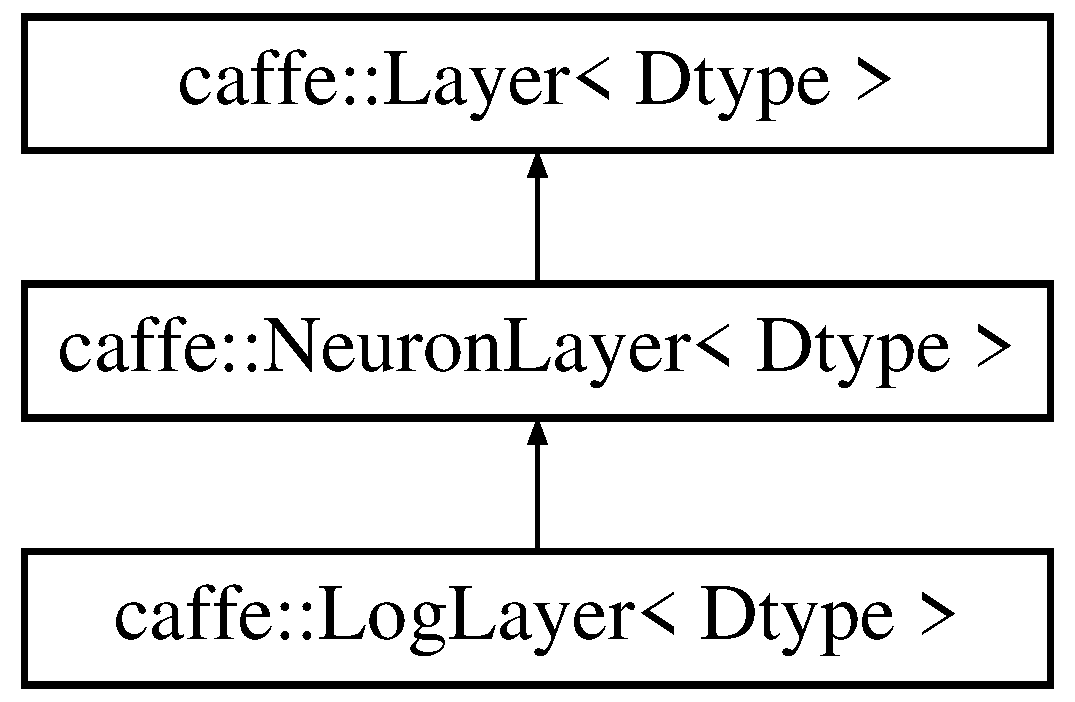
\includegraphics[height=3.000000cm]{classcaffe_1_1LogLayer}
\end{center}
\end{figure}
\subsection*{Public Member Functions}
\begin{DoxyCompactItemize}
\item 
\hyperlink{classcaffe_1_1LogLayer_aa6f92a0b12140d70a44a2bcb71bab552}{Log\+Layer} (const Layer\+Parameter \&param)
\item 
virtual void \hyperlink{classcaffe_1_1LogLayer_ab3f8854a38095f499e44ad8edf15b97b}{Layer\+Set\+Up} (const vector$<$ \hyperlink{classcaffe_1_1Blob}{Blob}$<$ Dtype $>$ $\ast$ $>$ \&bottom, const vector$<$ \hyperlink{classcaffe_1_1Blob}{Blob}$<$ Dtype $>$ $\ast$ $>$ \&top)
\begin{DoxyCompactList}\small\item\em Does layer-\/specific setup\+: your layer should implement this function as well as Reshape. \end{DoxyCompactList}\item 
virtual const char $\ast$ \hyperlink{classcaffe_1_1LogLayer_a35fe9f30bc494fb930aa0c7a19dadace}{type} () const \hypertarget{classcaffe_1_1LogLayer_a35fe9f30bc494fb930aa0c7a19dadace}{}\label{classcaffe_1_1LogLayer_a35fe9f30bc494fb930aa0c7a19dadace}

\begin{DoxyCompactList}\small\item\em Returns the layer type. \end{DoxyCompactList}\end{DoxyCompactItemize}
\subsection*{Protected Member Functions}
\begin{DoxyCompactItemize}
\item 
virtual void \hyperlink{classcaffe_1_1LogLayer_a928ac703824992b46eb33210e049fdb6}{Forward\+\_\+cpu} (const vector$<$ \hyperlink{classcaffe_1_1Blob}{Blob}$<$ Dtype $>$ $\ast$ $>$ \&bottom, const vector$<$ \hyperlink{classcaffe_1_1Blob}{Blob}$<$ Dtype $>$ $\ast$ $>$ \&top)
\item 
virtual void \hyperlink{classcaffe_1_1LogLayer_a6f9540e08387ce74287a6ee7abca8b1c}{Forward\+\_\+gpu} (const vector$<$ \hyperlink{classcaffe_1_1Blob}{Blob}$<$ Dtype $>$ $\ast$ $>$ \&bottom, const vector$<$ \hyperlink{classcaffe_1_1Blob}{Blob}$<$ Dtype $>$ $\ast$ $>$ \&top)\hypertarget{classcaffe_1_1LogLayer_a6f9540e08387ce74287a6ee7abca8b1c}{}\label{classcaffe_1_1LogLayer_a6f9540e08387ce74287a6ee7abca8b1c}

\begin{DoxyCompactList}\small\item\em Using the G\+PU device, compute the layer output. Fall back to \hyperlink{classcaffe_1_1LogLayer_a928ac703824992b46eb33210e049fdb6}{Forward\+\_\+cpu()} if unavailable. \end{DoxyCompactList}\item 
virtual void \hyperlink{classcaffe_1_1LogLayer_adde7e59f9b065e518e6f254c408eb3ef}{Backward\+\_\+cpu} (const vector$<$ \hyperlink{classcaffe_1_1Blob}{Blob}$<$ Dtype $>$ $\ast$ $>$ \&top, const vector$<$ bool $>$ \&propagate\+\_\+down, const vector$<$ \hyperlink{classcaffe_1_1Blob}{Blob}$<$ Dtype $>$ $\ast$ $>$ \&bottom)
\begin{DoxyCompactList}\small\item\em Computes the error gradient w.\+r.\+t. the exp inputs. \end{DoxyCompactList}\item 
virtual void \hyperlink{classcaffe_1_1LogLayer_ac4399854936b71196392d7736c162081}{Backward\+\_\+gpu} (const vector$<$ \hyperlink{classcaffe_1_1Blob}{Blob}$<$ Dtype $>$ $\ast$ $>$ \&top, const vector$<$ bool $>$ \&propagate\+\_\+down, const vector$<$ \hyperlink{classcaffe_1_1Blob}{Blob}$<$ Dtype $>$ $\ast$ $>$ \&bottom)\hypertarget{classcaffe_1_1LogLayer_ac4399854936b71196392d7736c162081}{}\label{classcaffe_1_1LogLayer_ac4399854936b71196392d7736c162081}

\begin{DoxyCompactList}\small\item\em Using the G\+PU device, compute the gradients for any parameters and for the bottom blobs if propagate\+\_\+down is true. Fall back to \hyperlink{classcaffe_1_1LogLayer_adde7e59f9b065e518e6f254c408eb3ef}{Backward\+\_\+cpu()} if unavailable. \end{DoxyCompactList}\end{DoxyCompactItemize}
\subsection*{Protected Attributes}
\begin{DoxyCompactItemize}
\item 
Dtype {\bfseries base\+\_\+scale\+\_\+}\hypertarget{classcaffe_1_1LogLayer_a491b3c774d06e7444e098f5e92116473}{}\label{classcaffe_1_1LogLayer_a491b3c774d06e7444e098f5e92116473}

\item 
Dtype {\bfseries input\+\_\+scale\+\_\+}\hypertarget{classcaffe_1_1LogLayer_a8c45b84ac085d9422655e68c107aa38f}{}\label{classcaffe_1_1LogLayer_a8c45b84ac085d9422655e68c107aa38f}

\item 
Dtype {\bfseries input\+\_\+shift\+\_\+}\hypertarget{classcaffe_1_1LogLayer_aea8ff4c75c4d1332801b91af479916af}{}\label{classcaffe_1_1LogLayer_aea8ff4c75c4d1332801b91af479916af}

\item 
Dtype {\bfseries backward\+\_\+num\+\_\+scale\+\_\+}\hypertarget{classcaffe_1_1LogLayer_ab87303089b3708884efaabef8a5e0df2}{}\label{classcaffe_1_1LogLayer_ab87303089b3708884efaabef8a5e0df2}

\end{DoxyCompactItemize}


\subsection{Detailed Description}
\subsubsection*{template$<$typename Dtype$>$\\*
class caffe\+::\+Log\+Layer$<$ Dtype $>$}

Computes $ y = log_{\gamma}(\alpha x + \beta) $, as specified by the scale $ \alpha $, shift $ \beta $, and base $ \gamma $. 

\subsection{Constructor \& Destructor Documentation}
\index{caffe\+::\+Log\+Layer@{caffe\+::\+Log\+Layer}!Log\+Layer@{Log\+Layer}}
\index{Log\+Layer@{Log\+Layer}!caffe\+::\+Log\+Layer@{caffe\+::\+Log\+Layer}}
\subsubsection[{\texorpdfstring{Log\+Layer(const Layer\+Parameter \&param)}{LogLayer(const LayerParameter &param)}}]{\setlength{\rightskip}{0pt plus 5cm}template$<$typename Dtype $>$ {\bf caffe\+::\+Log\+Layer}$<$ Dtype $>$\+::{\bf Log\+Layer} (
\begin{DoxyParamCaption}
\item[{const Layer\+Parameter \&}]{param}
\end{DoxyParamCaption}
)\hspace{0.3cm}{\ttfamily [inline]}, {\ttfamily [explicit]}}\hypertarget{classcaffe_1_1LogLayer_aa6f92a0b12140d70a44a2bcb71bab552}{}\label{classcaffe_1_1LogLayer_aa6f92a0b12140d70a44a2bcb71bab552}

\begin{DoxyParams}{Parameters}
{\em param} & provides Log\+Parameter log\+\_\+param, with \hyperlink{classcaffe_1_1LogLayer}{Log\+Layer} options\+:
\begin{DoxyItemize}
\item scale ({\bfseries optional}, default 1) the scale $ \alpha $
\item shift ({\bfseries optional}, default 0) the shift $ \beta $
\item base ({\bfseries optional}, default -\/1 for a value of $ e \approx 2.718 $) the base $ \gamma $ 
\end{DoxyItemize}\\
\hline
\end{DoxyParams}


\subsection{Member Function Documentation}
\index{caffe\+::\+Log\+Layer@{caffe\+::\+Log\+Layer}!Backward\+\_\+cpu@{Backward\+\_\+cpu}}
\index{Backward\+\_\+cpu@{Backward\+\_\+cpu}!caffe\+::\+Log\+Layer@{caffe\+::\+Log\+Layer}}
\subsubsection[{\texorpdfstring{Backward\+\_\+cpu(const vector$<$ Blob$<$ Dtype $>$ $\ast$ $>$ \&top, const vector$<$ bool $>$ \&propagate\+\_\+down, const vector$<$ Blob$<$ Dtype $>$ $\ast$ $>$ \&bottom)}{Backward_cpu(const vector< Blob< Dtype > * > &top, const vector< bool > &propagate_down, const vector< Blob< Dtype > * > &bottom)}}]{\setlength{\rightskip}{0pt plus 5cm}template$<$typename Dtype $>$ void {\bf caffe\+::\+Log\+Layer}$<$ Dtype $>$\+::Backward\+\_\+cpu (
\begin{DoxyParamCaption}
\item[{const vector$<$ {\bf Blob}$<$ Dtype $>$ $\ast$ $>$ \&}]{top, }
\item[{const vector$<$ bool $>$ \&}]{propagate\+\_\+down, }
\item[{const vector$<$ {\bf Blob}$<$ Dtype $>$ $\ast$ $>$ \&}]{bottom}
\end{DoxyParamCaption}
)\hspace{0.3cm}{\ttfamily [protected]}, {\ttfamily [virtual]}}\hypertarget{classcaffe_1_1LogLayer_adde7e59f9b065e518e6f254c408eb3ef}{}\label{classcaffe_1_1LogLayer_adde7e59f9b065e518e6f254c408eb3ef}


Computes the error gradient w.\+r.\+t. the exp inputs. 


\begin{DoxyParams}{Parameters}
{\em top} & output \hyperlink{classcaffe_1_1Blob}{Blob} vector (length 1), providing the error gradient with respect to the outputs
\begin{DoxyEnumerate}
\item $ (N \times C \times H \times W) $ containing error gradients $ \frac{\partial E}{\partial y} $ with respect to computed outputs $ y $ 
\end{DoxyEnumerate}\\
\hline
{\em propagate\+\_\+down} & see \hyperlink{classcaffe_1_1Layer_a53df1e081767e07bfb4c81657f4acd0a}{Layer\+::\+Backward}. \\
\hline
{\em bottom} & input \hyperlink{classcaffe_1_1Blob}{Blob} vector (length 1)
\begin{DoxyEnumerate}
\item $ (N \times C \times H \times W) $ the inputs $ x $; Backward fills their diff with gradients $ \frac{\partial E}{\partial x} = \frac{\partial E}{\partial y} y \alpha \log_e(gamma) $ if propagate\+\_\+down\mbox{[}0\mbox{]} 
\end{DoxyEnumerate}\\
\hline
\end{DoxyParams}


Implements \hyperlink{classcaffe_1_1Layer_a64d15855f882af4b82e83fa993c4e7c6}{caffe\+::\+Layer$<$ Dtype $>$}.

\index{caffe\+::\+Log\+Layer@{caffe\+::\+Log\+Layer}!Forward\+\_\+cpu@{Forward\+\_\+cpu}}
\index{Forward\+\_\+cpu@{Forward\+\_\+cpu}!caffe\+::\+Log\+Layer@{caffe\+::\+Log\+Layer}}
\subsubsection[{\texorpdfstring{Forward\+\_\+cpu(const vector$<$ Blob$<$ Dtype $>$ $\ast$ $>$ \&bottom, const vector$<$ Blob$<$ Dtype $>$ $\ast$ $>$ \&top)}{Forward_cpu(const vector< Blob< Dtype > * > &bottom, const vector< Blob< Dtype > * > &top)}}]{\setlength{\rightskip}{0pt plus 5cm}template$<$typename Dtype $>$ void {\bf caffe\+::\+Log\+Layer}$<$ Dtype $>$\+::Forward\+\_\+cpu (
\begin{DoxyParamCaption}
\item[{const vector$<$ {\bf Blob}$<$ Dtype $>$ $\ast$ $>$ \&}]{bottom, }
\item[{const vector$<$ {\bf Blob}$<$ Dtype $>$ $\ast$ $>$ \&}]{top}
\end{DoxyParamCaption}
)\hspace{0.3cm}{\ttfamily [protected]}, {\ttfamily [virtual]}}\hypertarget{classcaffe_1_1LogLayer_a928ac703824992b46eb33210e049fdb6}{}\label{classcaffe_1_1LogLayer_a928ac703824992b46eb33210e049fdb6}

\begin{DoxyParams}{Parameters}
{\em bottom} & input \hyperlink{classcaffe_1_1Blob}{Blob} vector (length 1)
\begin{DoxyEnumerate}
\item $ (N \times C \times H \times W) $ the inputs $ x $ 
\end{DoxyEnumerate}\\
\hline
{\em top} & output \hyperlink{classcaffe_1_1Blob}{Blob} vector (length 1)
\begin{DoxyEnumerate}
\item $ (N \times C \times H \times W) $ the computed outputs $ y = log_{\gamma}(\alpha x + \beta) $ 
\end{DoxyEnumerate}\\
\hline
\end{DoxyParams}


Implements \hyperlink{classcaffe_1_1Layer_add965883f75bbf90c7a06f960cda7a1a}{caffe\+::\+Layer$<$ Dtype $>$}.

\index{caffe\+::\+Log\+Layer@{caffe\+::\+Log\+Layer}!Layer\+Set\+Up@{Layer\+Set\+Up}}
\index{Layer\+Set\+Up@{Layer\+Set\+Up}!caffe\+::\+Log\+Layer@{caffe\+::\+Log\+Layer}}
\subsubsection[{\texorpdfstring{Layer\+Set\+Up(const vector$<$ Blob$<$ Dtype $>$ $\ast$ $>$ \&bottom, const vector$<$ Blob$<$ Dtype $>$ $\ast$ $>$ \&top)}{LayerSetUp(const vector< Blob< Dtype > * > &bottom, const vector< Blob< Dtype > * > &top)}}]{\setlength{\rightskip}{0pt plus 5cm}template$<$typename Dtype $>$ void {\bf caffe\+::\+Log\+Layer}$<$ Dtype $>$\+::Layer\+Set\+Up (
\begin{DoxyParamCaption}
\item[{const vector$<$ {\bf Blob}$<$ Dtype $>$ $\ast$ $>$ \&}]{bottom, }
\item[{const vector$<$ {\bf Blob}$<$ Dtype $>$ $\ast$ $>$ \&}]{top}
\end{DoxyParamCaption}
)\hspace{0.3cm}{\ttfamily [virtual]}}\hypertarget{classcaffe_1_1LogLayer_ab3f8854a38095f499e44ad8edf15b97b}{}\label{classcaffe_1_1LogLayer_ab3f8854a38095f499e44ad8edf15b97b}


Does layer-\/specific setup\+: your layer should implement this function as well as Reshape. 


\begin{DoxyParams}{Parameters}
{\em bottom} & the preshaped input blobs, whose data fields store the input data for this layer \\
\hline
{\em top} & the allocated but unshaped output blobs\\
\hline
\end{DoxyParams}
This method should do one-\/time layer specific setup. This includes reading and processing relevent parameters from the {\ttfamily layer\+\_\+param\+\_\+}. Setting up the shapes of top blobs and internal buffers should be done in {\ttfamily Reshape}, which will be called before the forward pass to adjust the top blob sizes. 

Reimplemented from \hyperlink{classcaffe_1_1Layer_a38dc2488bf319b8de5a7ac84e0045393}{caffe\+::\+Layer$<$ Dtype $>$}.



The documentation for this class was generated from the following files\+:\begin{DoxyCompactItemize}
\item 
include/caffe/layers/log\+\_\+layer.\+hpp\item 
src/caffe/layers/log\+\_\+layer.\+cpp\end{DoxyCompactItemize}

\hypertarget{classcaffe_1_1LossLayer}{}\section{caffe\+:\+:Loss\+Layer$<$ Dtype $>$ Class Template Reference}
\label{classcaffe_1_1LossLayer}\index{caffe\+::\+Loss\+Layer$<$ Dtype $>$@{caffe\+::\+Loss\+Layer$<$ Dtype $>$}}


An interface for \hyperlink{classcaffe_1_1Layer}{Layer}s that take two \hyperlink{classcaffe_1_1Blob}{Blob}s as input -- usually (1) predictions and (2) ground-\/truth labels -- and output a singleton \hyperlink{classcaffe_1_1Blob}{Blob} representing the loss.  




{\ttfamily \#include $<$loss\+\_\+layer.\+hpp$>$}

Inheritance diagram for caffe\+:\+:Loss\+Layer$<$ Dtype $>$\+:\begin{figure}[H]
\begin{center}
\leavevmode
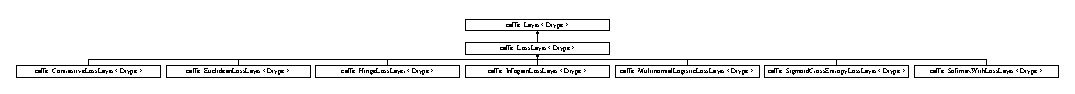
\includegraphics[height=0.821918cm]{classcaffe_1_1LossLayer}
\end{center}
\end{figure}
\subsection*{Public Member Functions}
\begin{DoxyCompactItemize}
\item 
{\bfseries Loss\+Layer} (const Layer\+Parameter \&param)\hypertarget{classcaffe_1_1LossLayer_a16e133050e2d97c6f024ea74e3ba4ead}{}\label{classcaffe_1_1LossLayer_a16e133050e2d97c6f024ea74e3ba4ead}

\item 
virtual void \hyperlink{classcaffe_1_1LossLayer_a98084e06f7ca0e44c11aee5544379609}{Layer\+Set\+Up} (const vector$<$ \hyperlink{classcaffe_1_1Blob}{Blob}$<$ Dtype $>$ $\ast$ $>$ \&bottom, const vector$<$ \hyperlink{classcaffe_1_1Blob}{Blob}$<$ Dtype $>$ $\ast$ $>$ \&top)
\begin{DoxyCompactList}\small\item\em Does layer-\/specific setup\+: your layer should implement this function as well as Reshape. \end{DoxyCompactList}\item 
virtual void \hyperlink{classcaffe_1_1LossLayer_ab15b7120ebc172274481f3732db78c9e}{Reshape} (const vector$<$ \hyperlink{classcaffe_1_1Blob}{Blob}$<$ Dtype $>$ $\ast$ $>$ \&bottom, const vector$<$ \hyperlink{classcaffe_1_1Blob}{Blob}$<$ Dtype $>$ $\ast$ $>$ \&top)
\begin{DoxyCompactList}\small\item\em Adjust the shapes of top blobs and internal buffers to accommodate the shapes of the bottom blobs. \end{DoxyCompactList}\item 
virtual int \hyperlink{classcaffe_1_1LossLayer_a8a2e16d4691640c34e589aac4ec42e28}{Exact\+Num\+Bottom\+Blobs} () const 
\begin{DoxyCompactList}\small\item\em Returns the exact number of bottom blobs required by the layer, or -\/1 if no exact number is required. \end{DoxyCompactList}\item 
virtual bool \hyperlink{classcaffe_1_1LossLayer_ad272e6792a781ce4f66a65057cc829d1}{Auto\+Top\+Blobs} () const \hypertarget{classcaffe_1_1LossLayer_ad272e6792a781ce4f66a65057cc829d1}{}\label{classcaffe_1_1LossLayer_ad272e6792a781ce4f66a65057cc829d1}

\begin{DoxyCompactList}\small\item\em For convenience and backwards compatibility, instruct the \hyperlink{classcaffe_1_1Net}{Net} to automatically allocate a single top \hyperlink{classcaffe_1_1Blob}{Blob} for Loss\+Layers, into which they output their singleton loss, (even if the user didn\textquotesingle{}t specify one in the prototxt, etc.). \end{DoxyCompactList}\item 
virtual int \hyperlink{classcaffe_1_1LossLayer_af8dca16967e8e979ebead4e80664dc10}{Exact\+Num\+Top\+Blobs} () const 
\begin{DoxyCompactList}\small\item\em Returns the exact number of top blobs required by the layer, or -\/1 if no exact number is required. \end{DoxyCompactList}\item 
virtual bool \hyperlink{classcaffe_1_1LossLayer_ad02fe695b06451ac8e6f21db0cba1dad}{Allow\+Force\+Backward} (const int bottom\+\_\+index) const 
\end{DoxyCompactItemize}
\subsection*{Additional Inherited Members}


\subsection{Detailed Description}
\subsubsection*{template$<$typename Dtype$>$\\*
class caffe\+::\+Loss\+Layer$<$ Dtype $>$}

An interface for \hyperlink{classcaffe_1_1Layer}{Layer}s that take two \hyperlink{classcaffe_1_1Blob}{Blob}s as input -- usually (1) predictions and (2) ground-\/truth labels -- and output a singleton \hyperlink{classcaffe_1_1Blob}{Blob} representing the loss. 

Loss\+Layers are typically only capable of backpropagating to their first input -- the predictions. 

\subsection{Member Function Documentation}
\index{caffe\+::\+Loss\+Layer@{caffe\+::\+Loss\+Layer}!Allow\+Force\+Backward@{Allow\+Force\+Backward}}
\index{Allow\+Force\+Backward@{Allow\+Force\+Backward}!caffe\+::\+Loss\+Layer@{caffe\+::\+Loss\+Layer}}
\subsubsection[{\texorpdfstring{Allow\+Force\+Backward(const int bottom\+\_\+index) const }{AllowForceBackward(const int bottom_index) const }}]{\setlength{\rightskip}{0pt plus 5cm}template$<$typename Dtype $>$ virtual bool {\bf caffe\+::\+Loss\+Layer}$<$ Dtype $>$\+::Allow\+Force\+Backward (
\begin{DoxyParamCaption}
\item[{const int}]{bottom\+\_\+index}
\end{DoxyParamCaption}
) const\hspace{0.3cm}{\ttfamily [inline]}, {\ttfamily [virtual]}}\hypertarget{classcaffe_1_1LossLayer_ad02fe695b06451ac8e6f21db0cba1dad}{}\label{classcaffe_1_1LossLayer_ad02fe695b06451ac8e6f21db0cba1dad}
We usually cannot backpropagate to the labels; ignore force\+\_\+backward for these inputs. 

Reimplemented from \hyperlink{classcaffe_1_1Layer_a4a2e4ca94eaa1cbc054b512c6657743e}{caffe\+::\+Layer$<$ Dtype $>$}.



Reimplemented in \hyperlink{classcaffe_1_1EuclideanLossLayer_a3c954fd7c15596fd2f59e0f79601905c}{caffe\+::\+Euclidean\+Loss\+Layer$<$ Dtype $>$}, and \hyperlink{classcaffe_1_1ContrastiveLossLayer_afbfe9d1707c9e76e31fe381af3d708ef}{caffe\+::\+Contrastive\+Loss\+Layer$<$ Dtype $>$}.

\index{caffe\+::\+Loss\+Layer@{caffe\+::\+Loss\+Layer}!Exact\+Num\+Bottom\+Blobs@{Exact\+Num\+Bottom\+Blobs}}
\index{Exact\+Num\+Bottom\+Blobs@{Exact\+Num\+Bottom\+Blobs}!caffe\+::\+Loss\+Layer@{caffe\+::\+Loss\+Layer}}
\subsubsection[{\texorpdfstring{Exact\+Num\+Bottom\+Blobs() const }{ExactNumBottomBlobs() const }}]{\setlength{\rightskip}{0pt plus 5cm}template$<$typename Dtype $>$ virtual int {\bf caffe\+::\+Loss\+Layer}$<$ Dtype $>$\+::Exact\+Num\+Bottom\+Blobs (
\begin{DoxyParamCaption}
{}
\end{DoxyParamCaption}
) const\hspace{0.3cm}{\ttfamily [inline]}, {\ttfamily [virtual]}}\hypertarget{classcaffe_1_1LossLayer_a8a2e16d4691640c34e589aac4ec42e28}{}\label{classcaffe_1_1LossLayer_a8a2e16d4691640c34e589aac4ec42e28}


Returns the exact number of bottom blobs required by the layer, or -\/1 if no exact number is required. 

This method should be overridden to return a non-\/negative value if your layer expects some exact number of bottom blobs. 

Reimplemented from \hyperlink{classcaffe_1_1Layer_a45c7a7943a8a6735ac433c9be11e0240}{caffe\+::\+Layer$<$ Dtype $>$}.



Reimplemented in \hyperlink{classcaffe_1_1InfogainLossLayer_aef9aa9200a3129d7bddf56f717017cbb}{caffe\+::\+Infogain\+Loss\+Layer$<$ Dtype $>$}, and \hyperlink{classcaffe_1_1ContrastiveLossLayer_af1b8bcaf8ddacd3e98e26c558c7f49a0}{caffe\+::\+Contrastive\+Loss\+Layer$<$ Dtype $>$}.

\index{caffe\+::\+Loss\+Layer@{caffe\+::\+Loss\+Layer}!Exact\+Num\+Top\+Blobs@{Exact\+Num\+Top\+Blobs}}
\index{Exact\+Num\+Top\+Blobs@{Exact\+Num\+Top\+Blobs}!caffe\+::\+Loss\+Layer@{caffe\+::\+Loss\+Layer}}
\subsubsection[{\texorpdfstring{Exact\+Num\+Top\+Blobs() const }{ExactNumTopBlobs() const }}]{\setlength{\rightskip}{0pt plus 5cm}template$<$typename Dtype $>$ virtual int {\bf caffe\+::\+Loss\+Layer}$<$ Dtype $>$\+::Exact\+Num\+Top\+Blobs (
\begin{DoxyParamCaption}
{}
\end{DoxyParamCaption}
) const\hspace{0.3cm}{\ttfamily [inline]}, {\ttfamily [virtual]}}\hypertarget{classcaffe_1_1LossLayer_af8dca16967e8e979ebead4e80664dc10}{}\label{classcaffe_1_1LossLayer_af8dca16967e8e979ebead4e80664dc10}


Returns the exact number of top blobs required by the layer, or -\/1 if no exact number is required. 

This method should be overridden to return a non-\/negative value if your layer expects some exact number of top blobs. 

Reimplemented from \hyperlink{classcaffe_1_1Layer_aa3c99ed707e8db683a3043412e151af8}{caffe\+::\+Layer$<$ Dtype $>$}.



Reimplemented in \hyperlink{classcaffe_1_1InfogainLossLayer_aa25f7b12805d10dccc217669f589fc95}{caffe\+::\+Infogain\+Loss\+Layer$<$ Dtype $>$}, and \hyperlink{classcaffe_1_1SoftmaxWithLossLayer_a8222589f986db56372bf00935bae6180}{caffe\+::\+Softmax\+With\+Loss\+Layer$<$ Dtype $>$}.

\index{caffe\+::\+Loss\+Layer@{caffe\+::\+Loss\+Layer}!Layer\+Set\+Up@{Layer\+Set\+Up}}
\index{Layer\+Set\+Up@{Layer\+Set\+Up}!caffe\+::\+Loss\+Layer@{caffe\+::\+Loss\+Layer}}
\subsubsection[{\texorpdfstring{Layer\+Set\+Up(const vector$<$ Blob$<$ Dtype $>$ $\ast$ $>$ \&bottom, const vector$<$ Blob$<$ Dtype $>$ $\ast$ $>$ \&top)}{LayerSetUp(const vector< Blob< Dtype > * > &bottom, const vector< Blob< Dtype > * > &top)}}]{\setlength{\rightskip}{0pt plus 5cm}template$<$typename Dtype $>$ void {\bf caffe\+::\+Loss\+Layer}$<$ Dtype $>$\+::Layer\+Set\+Up (
\begin{DoxyParamCaption}
\item[{const vector$<$ {\bf Blob}$<$ Dtype $>$ $\ast$ $>$ \&}]{bottom, }
\item[{const vector$<$ {\bf Blob}$<$ Dtype $>$ $\ast$ $>$ \&}]{top}
\end{DoxyParamCaption}
)\hspace{0.3cm}{\ttfamily [virtual]}}\hypertarget{classcaffe_1_1LossLayer_a98084e06f7ca0e44c11aee5544379609}{}\label{classcaffe_1_1LossLayer_a98084e06f7ca0e44c11aee5544379609}


Does layer-\/specific setup\+: your layer should implement this function as well as Reshape. 


\begin{DoxyParams}{Parameters}
{\em bottom} & the preshaped input blobs, whose data fields store the input data for this layer \\
\hline
{\em top} & the allocated but unshaped output blobs\\
\hline
\end{DoxyParams}
This method should do one-\/time layer specific setup. This includes reading and processing relevent parameters from the {\ttfamily layer\+\_\+param\+\_\+}. Setting up the shapes of top blobs and internal buffers should be done in {\ttfamily Reshape}, which will be called before the forward pass to adjust the top blob sizes. 

Reimplemented from \hyperlink{classcaffe_1_1Layer_a38dc2488bf319b8de5a7ac84e0045393}{caffe\+::\+Layer$<$ Dtype $>$}.



Reimplemented in \hyperlink{classcaffe_1_1SoftmaxWithLossLayer_a063c4e9786bc09f4773cb082c2960eb5}{caffe\+::\+Softmax\+With\+Loss\+Layer$<$ Dtype $>$}, \hyperlink{classcaffe_1_1InfogainLossLayer_a55a1d7ae2db81750c33ef9286764cd29}{caffe\+::\+Infogain\+Loss\+Layer$<$ Dtype $>$}, \hyperlink{classcaffe_1_1SigmoidCrossEntropyLossLayer_a87a48fa111fae84f238259d77263459e}{caffe\+::\+Sigmoid\+Cross\+Entropy\+Loss\+Layer$<$ Dtype $>$}, and \hyperlink{classcaffe_1_1ContrastiveLossLayer_a34a16b3e6598ec6c23e63c01ef0c0a99}{caffe\+::\+Contrastive\+Loss\+Layer$<$ Dtype $>$}.

\index{caffe\+::\+Loss\+Layer@{caffe\+::\+Loss\+Layer}!Reshape@{Reshape}}
\index{Reshape@{Reshape}!caffe\+::\+Loss\+Layer@{caffe\+::\+Loss\+Layer}}
\subsubsection[{\texorpdfstring{Reshape(const vector$<$ Blob$<$ Dtype $>$ $\ast$ $>$ \&bottom, const vector$<$ Blob$<$ Dtype $>$ $\ast$ $>$ \&top)}{Reshape(const vector< Blob< Dtype > * > &bottom, const vector< Blob< Dtype > * > &top)}}]{\setlength{\rightskip}{0pt plus 5cm}template$<$typename Dtype $>$ void {\bf caffe\+::\+Loss\+Layer}$<$ Dtype $>$\+::Reshape (
\begin{DoxyParamCaption}
\item[{const vector$<$ {\bf Blob}$<$ Dtype $>$ $\ast$ $>$ \&}]{bottom, }
\item[{const vector$<$ {\bf Blob}$<$ Dtype $>$ $\ast$ $>$ \&}]{top}
\end{DoxyParamCaption}
)\hspace{0.3cm}{\ttfamily [virtual]}}\hypertarget{classcaffe_1_1LossLayer_ab15b7120ebc172274481f3732db78c9e}{}\label{classcaffe_1_1LossLayer_ab15b7120ebc172274481f3732db78c9e}


Adjust the shapes of top blobs and internal buffers to accommodate the shapes of the bottom blobs. 


\begin{DoxyParams}{Parameters}
{\em bottom} & the input blobs, with the requested input shapes \\
\hline
{\em top} & the top blobs, which should be reshaped as needed\\
\hline
\end{DoxyParams}
This method should reshape top blobs as needed according to the shapes of the bottom (input) blobs, as well as reshaping any internal buffers and making any other necessary adjustments so that the layer can accommodate the bottom blobs. 

Implements \hyperlink{classcaffe_1_1Layer_ad9d391b972c769c0ebee34ca6d1c973e}{caffe\+::\+Layer$<$ Dtype $>$}.



Reimplemented in \hyperlink{classcaffe_1_1SoftmaxWithLossLayer_a9571f4e391a85f1b8b03aecbc47c298a}{caffe\+::\+Softmax\+With\+Loss\+Layer$<$ Dtype $>$}, \hyperlink{classcaffe_1_1InfogainLossLayer_aa1c32ab8252309cb51ed44cacf88f119}{caffe\+::\+Infogain\+Loss\+Layer$<$ Dtype $>$}, \hyperlink{classcaffe_1_1SigmoidCrossEntropyLossLayer_a81e7895b53040e8d56d03b5f52a9453f}{caffe\+::\+Sigmoid\+Cross\+Entropy\+Loss\+Layer$<$ Dtype $>$}, \hyperlink{classcaffe_1_1MultinomialLogisticLossLayer_a906947b9029c3ba8127591c49855ccb6}{caffe\+::\+Multinomial\+Logistic\+Loss\+Layer$<$ Dtype $>$}, and \hyperlink{classcaffe_1_1EuclideanLossLayer_a4d2df2fad6e3d04ed24df9fe6460c683}{caffe\+::\+Euclidean\+Loss\+Layer$<$ Dtype $>$}.



The documentation for this class was generated from the following files\+:\begin{DoxyCompactItemize}
\item 
include/caffe/layers/loss\+\_\+layer.\+hpp\item 
src/caffe/layers/loss\+\_\+layer.\+cpp\end{DoxyCompactItemize}

\hypertarget{classcaffe_1_1LRNLayer}{}\section{caffe\+:\+:L\+R\+N\+Layer$<$ Dtype $>$ Class Template Reference}
\label{classcaffe_1_1LRNLayer}\index{caffe\+::\+L\+R\+N\+Layer$<$ Dtype $>$@{caffe\+::\+L\+R\+N\+Layer$<$ Dtype $>$}}


Normalize the input in a local region across or within feature maps.  




{\ttfamily \#include $<$lrn\+\_\+layer.\+hpp$>$}

Inheritance diagram for caffe\+:\+:L\+R\+N\+Layer$<$ Dtype $>$\+:\begin{figure}[H]
\begin{center}
\leavevmode
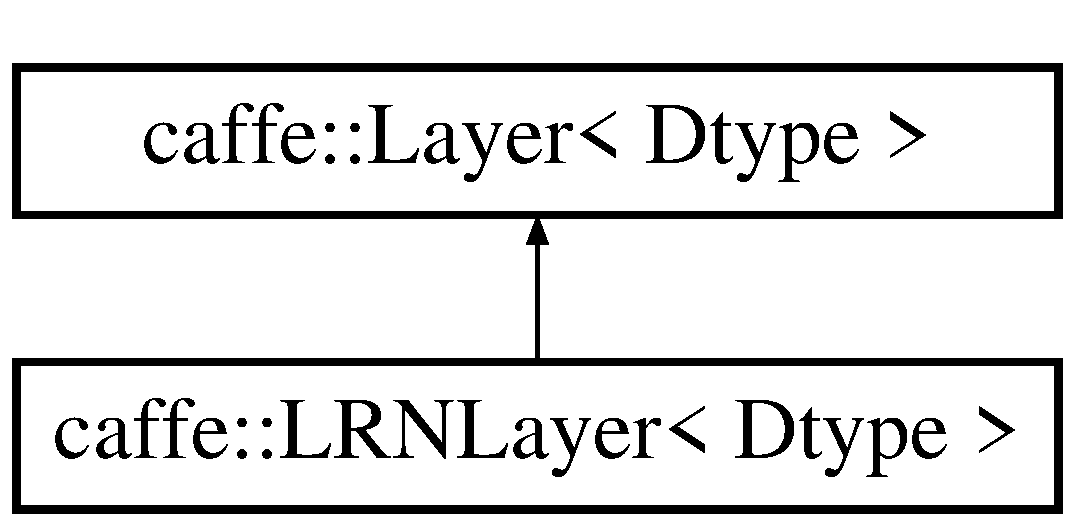
\includegraphics[height=2.000000cm]{classcaffe_1_1LRNLayer}
\end{center}
\end{figure}
\subsection*{Public Member Functions}
\begin{DoxyCompactItemize}
\item 
{\bfseries L\+R\+N\+Layer} (const Layer\+Parameter \&param)\hypertarget{classcaffe_1_1LRNLayer_a235b5f1b8fead8d1ddb9c29d627058fe}{}\label{classcaffe_1_1LRNLayer_a235b5f1b8fead8d1ddb9c29d627058fe}

\item 
virtual void \hyperlink{classcaffe_1_1LRNLayer_a7ab94b55392ad0500115d4a4d64b0a7c}{Layer\+Set\+Up} (const vector$<$ \hyperlink{classcaffe_1_1Blob}{Blob}$<$ Dtype $>$ $\ast$ $>$ \&bottom, const vector$<$ \hyperlink{classcaffe_1_1Blob}{Blob}$<$ Dtype $>$ $\ast$ $>$ \&top)
\begin{DoxyCompactList}\small\item\em Does layer-\/specific setup\+: your layer should implement this function as well as Reshape. \end{DoxyCompactList}\item 
virtual void \hyperlink{classcaffe_1_1LRNLayer_ae7ca62b2339f0691dadde24fd8acb481}{Reshape} (const vector$<$ \hyperlink{classcaffe_1_1Blob}{Blob}$<$ Dtype $>$ $\ast$ $>$ \&bottom, const vector$<$ \hyperlink{classcaffe_1_1Blob}{Blob}$<$ Dtype $>$ $\ast$ $>$ \&top)
\begin{DoxyCompactList}\small\item\em Adjust the shapes of top blobs and internal buffers to accommodate the shapes of the bottom blobs. \end{DoxyCompactList}\item 
virtual const char $\ast$ \hyperlink{classcaffe_1_1LRNLayer_a28dbd28c7542ae178973f0cb7b73cf8a}{type} () const \hypertarget{classcaffe_1_1LRNLayer_a28dbd28c7542ae178973f0cb7b73cf8a}{}\label{classcaffe_1_1LRNLayer_a28dbd28c7542ae178973f0cb7b73cf8a}

\begin{DoxyCompactList}\small\item\em Returns the layer type. \end{DoxyCompactList}\item 
virtual int \hyperlink{classcaffe_1_1LRNLayer_aabbbcdeb646c188ac2137b003aa1c682}{Exact\+Num\+Bottom\+Blobs} () const 
\begin{DoxyCompactList}\small\item\em Returns the exact number of bottom blobs required by the layer, or -\/1 if no exact number is required. \end{DoxyCompactList}\item 
virtual int \hyperlink{classcaffe_1_1LRNLayer_aab9056708727154a01866d17756c07cc}{Exact\+Num\+Top\+Blobs} () const 
\begin{DoxyCompactList}\small\item\em Returns the exact number of top blobs required by the layer, or -\/1 if no exact number is required. \end{DoxyCompactList}\end{DoxyCompactItemize}
\subsection*{Protected Member Functions}
\begin{DoxyCompactItemize}
\item 
virtual void \hyperlink{classcaffe_1_1LRNLayer_ad3ae42eb16a0f55745211a44c806e316}{Forward\+\_\+cpu} (const vector$<$ \hyperlink{classcaffe_1_1Blob}{Blob}$<$ Dtype $>$ $\ast$ $>$ \&bottom, const vector$<$ \hyperlink{classcaffe_1_1Blob}{Blob}$<$ Dtype $>$ $\ast$ $>$ \&top)\hypertarget{classcaffe_1_1LRNLayer_ad3ae42eb16a0f55745211a44c806e316}{}\label{classcaffe_1_1LRNLayer_ad3ae42eb16a0f55745211a44c806e316}

\begin{DoxyCompactList}\small\item\em Using the C\+PU device, compute the layer output. \end{DoxyCompactList}\item 
virtual void \hyperlink{classcaffe_1_1LRNLayer_a7d8e7e7e1daf4ae1205e0bfe9fb9ac51}{Forward\+\_\+gpu} (const vector$<$ \hyperlink{classcaffe_1_1Blob}{Blob}$<$ Dtype $>$ $\ast$ $>$ \&bottom, const vector$<$ \hyperlink{classcaffe_1_1Blob}{Blob}$<$ Dtype $>$ $\ast$ $>$ \&top)\hypertarget{classcaffe_1_1LRNLayer_a7d8e7e7e1daf4ae1205e0bfe9fb9ac51}{}\label{classcaffe_1_1LRNLayer_a7d8e7e7e1daf4ae1205e0bfe9fb9ac51}

\begin{DoxyCompactList}\small\item\em Using the G\+PU device, compute the layer output. Fall back to \hyperlink{classcaffe_1_1LRNLayer_ad3ae42eb16a0f55745211a44c806e316}{Forward\+\_\+cpu()} if unavailable. \end{DoxyCompactList}\item 
virtual void \hyperlink{classcaffe_1_1LRNLayer_a71ff30a634527e2bf89c067d3c325979}{Backward\+\_\+cpu} (const vector$<$ \hyperlink{classcaffe_1_1Blob}{Blob}$<$ Dtype $>$ $\ast$ $>$ \&top, const vector$<$ bool $>$ \&propagate\+\_\+down, const vector$<$ \hyperlink{classcaffe_1_1Blob}{Blob}$<$ Dtype $>$ $\ast$ $>$ \&bottom)\hypertarget{classcaffe_1_1LRNLayer_a71ff30a634527e2bf89c067d3c325979}{}\label{classcaffe_1_1LRNLayer_a71ff30a634527e2bf89c067d3c325979}

\begin{DoxyCompactList}\small\item\em Using the C\+PU device, compute the gradients for any parameters and for the bottom blobs if propagate\+\_\+down is true. \end{DoxyCompactList}\item 
virtual void \hyperlink{classcaffe_1_1LRNLayer_a1ba7e8a8af945fba73da4a0c307fc4a0}{Backward\+\_\+gpu} (const vector$<$ \hyperlink{classcaffe_1_1Blob}{Blob}$<$ Dtype $>$ $\ast$ $>$ \&top, const vector$<$ bool $>$ \&propagate\+\_\+down, const vector$<$ \hyperlink{classcaffe_1_1Blob}{Blob}$<$ Dtype $>$ $\ast$ $>$ \&bottom)\hypertarget{classcaffe_1_1LRNLayer_a1ba7e8a8af945fba73da4a0c307fc4a0}{}\label{classcaffe_1_1LRNLayer_a1ba7e8a8af945fba73da4a0c307fc4a0}

\begin{DoxyCompactList}\small\item\em Using the G\+PU device, compute the gradients for any parameters and for the bottom blobs if propagate\+\_\+down is true. Fall back to \hyperlink{classcaffe_1_1LRNLayer_a71ff30a634527e2bf89c067d3c325979}{Backward\+\_\+cpu()} if unavailable. \end{DoxyCompactList}\item 
virtual void {\bfseries Cross\+Channel\+Forward\+\_\+cpu} (const vector$<$ \hyperlink{classcaffe_1_1Blob}{Blob}$<$ Dtype $>$ $\ast$ $>$ \&bottom, const vector$<$ \hyperlink{classcaffe_1_1Blob}{Blob}$<$ Dtype $>$ $\ast$ $>$ \&top)\hypertarget{classcaffe_1_1LRNLayer_a9245d2e182710f0bc7bb637eda6deb65}{}\label{classcaffe_1_1LRNLayer_a9245d2e182710f0bc7bb637eda6deb65}

\item 
virtual void {\bfseries Cross\+Channel\+Forward\+\_\+gpu} (const vector$<$ \hyperlink{classcaffe_1_1Blob}{Blob}$<$ Dtype $>$ $\ast$ $>$ \&bottom, const vector$<$ \hyperlink{classcaffe_1_1Blob}{Blob}$<$ Dtype $>$ $\ast$ $>$ \&top)\hypertarget{classcaffe_1_1LRNLayer_adb64964f9adf8f7fd2f51e079de94e71}{}\label{classcaffe_1_1LRNLayer_adb64964f9adf8f7fd2f51e079de94e71}

\item 
virtual void {\bfseries Within\+Channel\+Forward} (const vector$<$ \hyperlink{classcaffe_1_1Blob}{Blob}$<$ Dtype $>$ $\ast$ $>$ \&bottom, const vector$<$ \hyperlink{classcaffe_1_1Blob}{Blob}$<$ Dtype $>$ $\ast$ $>$ \&top)\hypertarget{classcaffe_1_1LRNLayer_a1ee0b177676121e682bdfa02f9156efe}{}\label{classcaffe_1_1LRNLayer_a1ee0b177676121e682bdfa02f9156efe}

\item 
virtual void {\bfseries Cross\+Channel\+Backward\+\_\+cpu} (const vector$<$ \hyperlink{classcaffe_1_1Blob}{Blob}$<$ Dtype $>$ $\ast$ $>$ \&top, const vector$<$ bool $>$ \&propagate\+\_\+down, const vector$<$ \hyperlink{classcaffe_1_1Blob}{Blob}$<$ Dtype $>$ $\ast$ $>$ \&bottom)\hypertarget{classcaffe_1_1LRNLayer_acf4dbe14f7287924309aefa95cfc3273}{}\label{classcaffe_1_1LRNLayer_acf4dbe14f7287924309aefa95cfc3273}

\item 
virtual void {\bfseries Cross\+Channel\+Backward\+\_\+gpu} (const vector$<$ \hyperlink{classcaffe_1_1Blob}{Blob}$<$ Dtype $>$ $\ast$ $>$ \&top, const vector$<$ bool $>$ \&propagate\+\_\+down, const vector$<$ \hyperlink{classcaffe_1_1Blob}{Blob}$<$ Dtype $>$ $\ast$ $>$ \&bottom)\hypertarget{classcaffe_1_1LRNLayer_af20fe643394acab7d522b5486e7d18af}{}\label{classcaffe_1_1LRNLayer_af20fe643394acab7d522b5486e7d18af}

\item 
virtual void {\bfseries Within\+Channel\+Backward} (const vector$<$ \hyperlink{classcaffe_1_1Blob}{Blob}$<$ Dtype $>$ $\ast$ $>$ \&top, const vector$<$ bool $>$ \&propagate\+\_\+down, const vector$<$ \hyperlink{classcaffe_1_1Blob}{Blob}$<$ Dtype $>$ $\ast$ $>$ \&bottom)\hypertarget{classcaffe_1_1LRNLayer_af2e2a6f5d01e8add2d297b5437f33d49}{}\label{classcaffe_1_1LRNLayer_af2e2a6f5d01e8add2d297b5437f33d49}

\end{DoxyCompactItemize}
\subsection*{Protected Attributes}
\begin{DoxyCompactItemize}
\item 
int {\bfseries size\+\_\+}\hypertarget{classcaffe_1_1LRNLayer_a4d74c3370e28abe013bf0fcc815fcc17}{}\label{classcaffe_1_1LRNLayer_a4d74c3370e28abe013bf0fcc815fcc17}

\item 
int {\bfseries pre\+\_\+pad\+\_\+}\hypertarget{classcaffe_1_1LRNLayer_a5d4a63f1279542a4fbe2780ba061f800}{}\label{classcaffe_1_1LRNLayer_a5d4a63f1279542a4fbe2780ba061f800}

\item 
Dtype {\bfseries alpha\+\_\+}\hypertarget{classcaffe_1_1LRNLayer_ae5a9eaf89e4082afe166f0fa7ee3b4ed}{}\label{classcaffe_1_1LRNLayer_ae5a9eaf89e4082afe166f0fa7ee3b4ed}

\item 
Dtype {\bfseries beta\+\_\+}\hypertarget{classcaffe_1_1LRNLayer_aa0765abb189bb6be067494ea5cc925f2}{}\label{classcaffe_1_1LRNLayer_aa0765abb189bb6be067494ea5cc925f2}

\item 
Dtype {\bfseries k\+\_\+}\hypertarget{classcaffe_1_1LRNLayer_a2fd6dd95ba02ae082bf5668305f19844}{}\label{classcaffe_1_1LRNLayer_a2fd6dd95ba02ae082bf5668305f19844}

\item 
int {\bfseries num\+\_\+}\hypertarget{classcaffe_1_1LRNLayer_ac68d88464a09f9deaf929908ffbaf345}{}\label{classcaffe_1_1LRNLayer_ac68d88464a09f9deaf929908ffbaf345}

\item 
int {\bfseries channels\+\_\+}\hypertarget{classcaffe_1_1LRNLayer_acd1bc62c5c9074c1df80f12d716f9a7a}{}\label{classcaffe_1_1LRNLayer_acd1bc62c5c9074c1df80f12d716f9a7a}

\item 
int {\bfseries height\+\_\+}\hypertarget{classcaffe_1_1LRNLayer_a9fa09286b061a99713b4268259fdaad7}{}\label{classcaffe_1_1LRNLayer_a9fa09286b061a99713b4268259fdaad7}

\item 
int {\bfseries width\+\_\+}\hypertarget{classcaffe_1_1LRNLayer_a5b12d5c779f16e9b1caf4c3a6d581e09}{}\label{classcaffe_1_1LRNLayer_a5b12d5c779f16e9b1caf4c3a6d581e09}

\item 
\hyperlink{classcaffe_1_1Blob}{Blob}$<$ Dtype $>$ {\bfseries scale\+\_\+}\hypertarget{classcaffe_1_1LRNLayer_a61a44943c15c502c557df755d8ef4c6c}{}\label{classcaffe_1_1LRNLayer_a61a44943c15c502c557df755d8ef4c6c}

\item 
shared\+\_\+ptr$<$ \hyperlink{classcaffe_1_1SplitLayer}{Split\+Layer}$<$ Dtype $>$ $>$ {\bfseries split\+\_\+layer\+\_\+}\hypertarget{classcaffe_1_1LRNLayer_a7126b6cbb83ddafb80c9d9dc6d44f88f}{}\label{classcaffe_1_1LRNLayer_a7126b6cbb83ddafb80c9d9dc6d44f88f}

\item 
vector$<$ \hyperlink{classcaffe_1_1Blob}{Blob}$<$ Dtype $>$ $\ast$ $>$ {\bfseries split\+\_\+top\+\_\+vec\+\_\+}\hypertarget{classcaffe_1_1LRNLayer_a9b199156b8113800365c64c22e0e177a}{}\label{classcaffe_1_1LRNLayer_a9b199156b8113800365c64c22e0e177a}

\item 
shared\+\_\+ptr$<$ \hyperlink{classcaffe_1_1PowerLayer}{Power\+Layer}$<$ Dtype $>$ $>$ {\bfseries square\+\_\+layer\+\_\+}\hypertarget{classcaffe_1_1LRNLayer_a440a40fc6ec9131fd8425dabe8a48fa9}{}\label{classcaffe_1_1LRNLayer_a440a40fc6ec9131fd8425dabe8a48fa9}

\item 
\hyperlink{classcaffe_1_1Blob}{Blob}$<$ Dtype $>$ {\bfseries square\+\_\+input\+\_\+}\hypertarget{classcaffe_1_1LRNLayer_a750c4b6871af300f8de03b5eda197056}{}\label{classcaffe_1_1LRNLayer_a750c4b6871af300f8de03b5eda197056}

\item 
\hyperlink{classcaffe_1_1Blob}{Blob}$<$ Dtype $>$ {\bfseries square\+\_\+output\+\_\+}\hypertarget{classcaffe_1_1LRNLayer_a50c1f72f225f69d344857fc55dc52ef9}{}\label{classcaffe_1_1LRNLayer_a50c1f72f225f69d344857fc55dc52ef9}

\item 
vector$<$ \hyperlink{classcaffe_1_1Blob}{Blob}$<$ Dtype $>$ $\ast$ $>$ {\bfseries square\+\_\+bottom\+\_\+vec\+\_\+}\hypertarget{classcaffe_1_1LRNLayer_a0361883b2eada25a56b5a90f5ff99cac}{}\label{classcaffe_1_1LRNLayer_a0361883b2eada25a56b5a90f5ff99cac}

\item 
vector$<$ \hyperlink{classcaffe_1_1Blob}{Blob}$<$ Dtype $>$ $\ast$ $>$ {\bfseries square\+\_\+top\+\_\+vec\+\_\+}\hypertarget{classcaffe_1_1LRNLayer_accfb1597e6045b09dcdb421ba7e92070}{}\label{classcaffe_1_1LRNLayer_accfb1597e6045b09dcdb421ba7e92070}

\item 
shared\+\_\+ptr$<$ \hyperlink{classcaffe_1_1PoolingLayer}{Pooling\+Layer}$<$ Dtype $>$ $>$ {\bfseries pool\+\_\+layer\+\_\+}\hypertarget{classcaffe_1_1LRNLayer_a3d883b2d7022bd66e1ac2227400a1caa}{}\label{classcaffe_1_1LRNLayer_a3d883b2d7022bd66e1ac2227400a1caa}

\item 
\hyperlink{classcaffe_1_1Blob}{Blob}$<$ Dtype $>$ {\bfseries pool\+\_\+output\+\_\+}\hypertarget{classcaffe_1_1LRNLayer_a7dfcd31ed9694bdd48c9e80bdfe1e7a4}{}\label{classcaffe_1_1LRNLayer_a7dfcd31ed9694bdd48c9e80bdfe1e7a4}

\item 
vector$<$ \hyperlink{classcaffe_1_1Blob}{Blob}$<$ Dtype $>$ $\ast$ $>$ {\bfseries pool\+\_\+top\+\_\+vec\+\_\+}\hypertarget{classcaffe_1_1LRNLayer_af1d75143e7d103749575c3ee167e1c8d}{}\label{classcaffe_1_1LRNLayer_af1d75143e7d103749575c3ee167e1c8d}

\item 
shared\+\_\+ptr$<$ \hyperlink{classcaffe_1_1PowerLayer}{Power\+Layer}$<$ Dtype $>$ $>$ {\bfseries power\+\_\+layer\+\_\+}\hypertarget{classcaffe_1_1LRNLayer_a7d9446e995a4e4d1c27961159c1e7950}{}\label{classcaffe_1_1LRNLayer_a7d9446e995a4e4d1c27961159c1e7950}

\item 
\hyperlink{classcaffe_1_1Blob}{Blob}$<$ Dtype $>$ {\bfseries power\+\_\+output\+\_\+}\hypertarget{classcaffe_1_1LRNLayer_adb51a5bb10b26a27835b2b19ecfe72b2}{}\label{classcaffe_1_1LRNLayer_adb51a5bb10b26a27835b2b19ecfe72b2}

\item 
vector$<$ \hyperlink{classcaffe_1_1Blob}{Blob}$<$ Dtype $>$ $\ast$ $>$ {\bfseries power\+\_\+top\+\_\+vec\+\_\+}\hypertarget{classcaffe_1_1LRNLayer_ac83227b50de568833235e7b2bdfbb8a8}{}\label{classcaffe_1_1LRNLayer_ac83227b50de568833235e7b2bdfbb8a8}

\item 
shared\+\_\+ptr$<$ \hyperlink{classcaffe_1_1EltwiseLayer}{Eltwise\+Layer}$<$ Dtype $>$ $>$ {\bfseries product\+\_\+layer\+\_\+}\hypertarget{classcaffe_1_1LRNLayer_a83ee2091c7f93f72cec177d98124b16f}{}\label{classcaffe_1_1LRNLayer_a83ee2091c7f93f72cec177d98124b16f}

\item 
\hyperlink{classcaffe_1_1Blob}{Blob}$<$ Dtype $>$ {\bfseries product\+\_\+input\+\_\+}\hypertarget{classcaffe_1_1LRNLayer_aff284ba9f23d00aefa62759ee50b7253}{}\label{classcaffe_1_1LRNLayer_aff284ba9f23d00aefa62759ee50b7253}

\item 
vector$<$ \hyperlink{classcaffe_1_1Blob}{Blob}$<$ Dtype $>$ $\ast$ $>$ {\bfseries product\+\_\+bottom\+\_\+vec\+\_\+}\hypertarget{classcaffe_1_1LRNLayer_ab1bf581b7cf42b36bdbad8333989a177}{}\label{classcaffe_1_1LRNLayer_ab1bf581b7cf42b36bdbad8333989a177}

\end{DoxyCompactItemize}


\subsection{Detailed Description}
\subsubsection*{template$<$typename Dtype$>$\\*
class caffe\+::\+L\+R\+N\+Layer$<$ Dtype $>$}

Normalize the input in a local region across or within feature maps. 

T\+O\+D\+O(dox)\+: thorough documentation for Forward, Backward, and proto params. 

\subsection{Member Function Documentation}
\index{caffe\+::\+L\+R\+N\+Layer@{caffe\+::\+L\+R\+N\+Layer}!Exact\+Num\+Bottom\+Blobs@{Exact\+Num\+Bottom\+Blobs}}
\index{Exact\+Num\+Bottom\+Blobs@{Exact\+Num\+Bottom\+Blobs}!caffe\+::\+L\+R\+N\+Layer@{caffe\+::\+L\+R\+N\+Layer}}
\subsubsection[{\texorpdfstring{Exact\+Num\+Bottom\+Blobs() const }{ExactNumBottomBlobs() const }}]{\setlength{\rightskip}{0pt plus 5cm}template$<$typename Dtype $>$ virtual int {\bf caffe\+::\+L\+R\+N\+Layer}$<$ Dtype $>$\+::Exact\+Num\+Bottom\+Blobs (
\begin{DoxyParamCaption}
{}
\end{DoxyParamCaption}
) const\hspace{0.3cm}{\ttfamily [inline]}, {\ttfamily [virtual]}}\hypertarget{classcaffe_1_1LRNLayer_aabbbcdeb646c188ac2137b003aa1c682}{}\label{classcaffe_1_1LRNLayer_aabbbcdeb646c188ac2137b003aa1c682}


Returns the exact number of bottom blobs required by the layer, or -\/1 if no exact number is required. 

This method should be overridden to return a non-\/negative value if your layer expects some exact number of bottom blobs. 

Reimplemented from \hyperlink{classcaffe_1_1Layer_a45c7a7943a8a6735ac433c9be11e0240}{caffe\+::\+Layer$<$ Dtype $>$}.

\index{caffe\+::\+L\+R\+N\+Layer@{caffe\+::\+L\+R\+N\+Layer}!Exact\+Num\+Top\+Blobs@{Exact\+Num\+Top\+Blobs}}
\index{Exact\+Num\+Top\+Blobs@{Exact\+Num\+Top\+Blobs}!caffe\+::\+L\+R\+N\+Layer@{caffe\+::\+L\+R\+N\+Layer}}
\subsubsection[{\texorpdfstring{Exact\+Num\+Top\+Blobs() const }{ExactNumTopBlobs() const }}]{\setlength{\rightskip}{0pt plus 5cm}template$<$typename Dtype $>$ virtual int {\bf caffe\+::\+L\+R\+N\+Layer}$<$ Dtype $>$\+::Exact\+Num\+Top\+Blobs (
\begin{DoxyParamCaption}
{}
\end{DoxyParamCaption}
) const\hspace{0.3cm}{\ttfamily [inline]}, {\ttfamily [virtual]}}\hypertarget{classcaffe_1_1LRNLayer_aab9056708727154a01866d17756c07cc}{}\label{classcaffe_1_1LRNLayer_aab9056708727154a01866d17756c07cc}


Returns the exact number of top blobs required by the layer, or -\/1 if no exact number is required. 

This method should be overridden to return a non-\/negative value if your layer expects some exact number of top blobs. 

Reimplemented from \hyperlink{classcaffe_1_1Layer_aa3c99ed707e8db683a3043412e151af8}{caffe\+::\+Layer$<$ Dtype $>$}.

\index{caffe\+::\+L\+R\+N\+Layer@{caffe\+::\+L\+R\+N\+Layer}!Layer\+Set\+Up@{Layer\+Set\+Up}}
\index{Layer\+Set\+Up@{Layer\+Set\+Up}!caffe\+::\+L\+R\+N\+Layer@{caffe\+::\+L\+R\+N\+Layer}}
\subsubsection[{\texorpdfstring{Layer\+Set\+Up(const vector$<$ Blob$<$ Dtype $>$ $\ast$ $>$ \&bottom, const vector$<$ Blob$<$ Dtype $>$ $\ast$ $>$ \&top)}{LayerSetUp(const vector< Blob< Dtype > * > &bottom, const vector< Blob< Dtype > * > &top)}}]{\setlength{\rightskip}{0pt plus 5cm}template$<$typename Dtype $>$ void {\bf caffe\+::\+L\+R\+N\+Layer}$<$ Dtype $>$\+::Layer\+Set\+Up (
\begin{DoxyParamCaption}
\item[{const vector$<$ {\bf Blob}$<$ Dtype $>$ $\ast$ $>$ \&}]{bottom, }
\item[{const vector$<$ {\bf Blob}$<$ Dtype $>$ $\ast$ $>$ \&}]{top}
\end{DoxyParamCaption}
)\hspace{0.3cm}{\ttfamily [virtual]}}\hypertarget{classcaffe_1_1LRNLayer_a7ab94b55392ad0500115d4a4d64b0a7c}{}\label{classcaffe_1_1LRNLayer_a7ab94b55392ad0500115d4a4d64b0a7c}


Does layer-\/specific setup\+: your layer should implement this function as well as Reshape. 


\begin{DoxyParams}{Parameters}
{\em bottom} & the preshaped input blobs, whose data fields store the input data for this layer \\
\hline
{\em top} & the allocated but unshaped output blobs\\
\hline
\end{DoxyParams}
This method should do one-\/time layer specific setup. This includes reading and processing relevent parameters from the {\ttfamily layer\+\_\+param\+\_\+}. Setting up the shapes of top blobs and internal buffers should be done in {\ttfamily Reshape}, which will be called before the forward pass to adjust the top blob sizes. 

Reimplemented from \hyperlink{classcaffe_1_1Layer_a38dc2488bf319b8de5a7ac84e0045393}{caffe\+::\+Layer$<$ Dtype $>$}.

\index{caffe\+::\+L\+R\+N\+Layer@{caffe\+::\+L\+R\+N\+Layer}!Reshape@{Reshape}}
\index{Reshape@{Reshape}!caffe\+::\+L\+R\+N\+Layer@{caffe\+::\+L\+R\+N\+Layer}}
\subsubsection[{\texorpdfstring{Reshape(const vector$<$ Blob$<$ Dtype $>$ $\ast$ $>$ \&bottom, const vector$<$ Blob$<$ Dtype $>$ $\ast$ $>$ \&top)}{Reshape(const vector< Blob< Dtype > * > &bottom, const vector< Blob< Dtype > * > &top)}}]{\setlength{\rightskip}{0pt plus 5cm}template$<$typename Dtype $>$ void {\bf caffe\+::\+L\+R\+N\+Layer}$<$ Dtype $>$\+::Reshape (
\begin{DoxyParamCaption}
\item[{const vector$<$ {\bf Blob}$<$ Dtype $>$ $\ast$ $>$ \&}]{bottom, }
\item[{const vector$<$ {\bf Blob}$<$ Dtype $>$ $\ast$ $>$ \&}]{top}
\end{DoxyParamCaption}
)\hspace{0.3cm}{\ttfamily [virtual]}}\hypertarget{classcaffe_1_1LRNLayer_ae7ca62b2339f0691dadde24fd8acb481}{}\label{classcaffe_1_1LRNLayer_ae7ca62b2339f0691dadde24fd8acb481}


Adjust the shapes of top blobs and internal buffers to accommodate the shapes of the bottom blobs. 


\begin{DoxyParams}{Parameters}
{\em bottom} & the input blobs, with the requested input shapes \\
\hline
{\em top} & the top blobs, which should be reshaped as needed\\
\hline
\end{DoxyParams}
This method should reshape top blobs as needed according to the shapes of the bottom (input) blobs, as well as reshaping any internal buffers and making any other necessary adjustments so that the layer can accommodate the bottom blobs. 

Implements \hyperlink{classcaffe_1_1Layer_ad9d391b972c769c0ebee34ca6d1c973e}{caffe\+::\+Layer$<$ Dtype $>$}.



The documentation for this class was generated from the following files\+:\begin{DoxyCompactItemize}
\item 
include/caffe/layers/lrn\+\_\+layer.\+hpp\item 
src/caffe/layers/lrn\+\_\+layer.\+cpp\end{DoxyCompactItemize}

\hypertarget{classcaffe_1_1LSTMLayer}{}\section{caffe\+:\+:L\+S\+T\+M\+Layer$<$ Dtype $>$ Class Template Reference}
\label{classcaffe_1_1LSTMLayer}\index{caffe\+::\+L\+S\+T\+M\+Layer$<$ Dtype $>$@{caffe\+::\+L\+S\+T\+M\+Layer$<$ Dtype $>$}}


Processes sequential inputs using a \char`\"{}\+Long Short-\/\+Term Memory\char`\"{} (L\+S\+TM) \mbox{[}1\mbox{]} style recurrent neural network (R\+NN). Implemented by unrolling the L\+S\+TM computation through time.  




{\ttfamily \#include $<$lstm\+\_\+layer.\+hpp$>$}

Inheritance diagram for caffe\+:\+:L\+S\+T\+M\+Layer$<$ Dtype $>$\+:\begin{figure}[H]
\begin{center}
\leavevmode
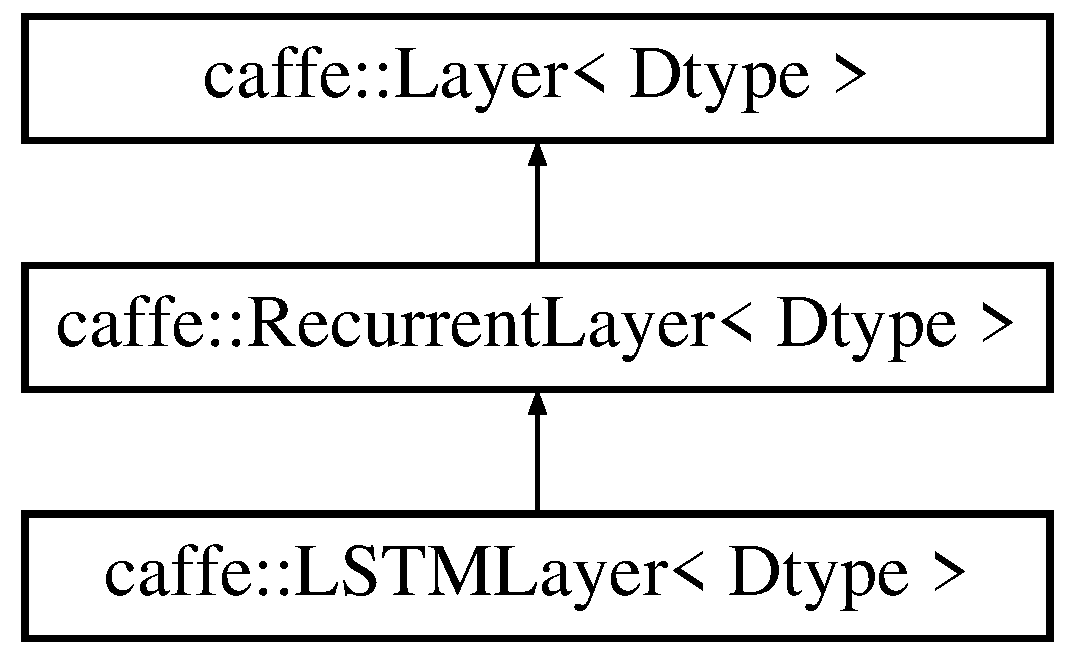
\includegraphics[height=3.000000cm]{classcaffe_1_1LSTMLayer}
\end{center}
\end{figure}
\subsection*{Public Member Functions}
\begin{DoxyCompactItemize}
\item 
{\bfseries L\+S\+T\+M\+Layer} (const Layer\+Parameter \&param)\hypertarget{classcaffe_1_1LSTMLayer_abcf1a46aef1f25b7a78d13dc7e34f13b}{}\label{classcaffe_1_1LSTMLayer_abcf1a46aef1f25b7a78d13dc7e34f13b}

\item 
virtual const char $\ast$ \hyperlink{classcaffe_1_1LSTMLayer_ab427faecd6e35031780a6146df62b1c5}{type} () const \hypertarget{classcaffe_1_1LSTMLayer_ab427faecd6e35031780a6146df62b1c5}{}\label{classcaffe_1_1LSTMLayer_ab427faecd6e35031780a6146df62b1c5}

\begin{DoxyCompactList}\small\item\em Returns the layer type. \end{DoxyCompactList}\end{DoxyCompactItemize}
\subsection*{Protected Member Functions}
\begin{DoxyCompactItemize}
\item 
virtual void \hyperlink{classcaffe_1_1LSTMLayer_aee83b6364883ffcb8f2c15a18a3031ac}{Fill\+Unrolled\+Net} (Net\+Parameter $\ast$net\+\_\+param) const \hypertarget{classcaffe_1_1LSTMLayer_aee83b6364883ffcb8f2c15a18a3031ac}{}\label{classcaffe_1_1LSTMLayer_aee83b6364883ffcb8f2c15a18a3031ac}

\begin{DoxyCompactList}\small\item\em Fills net\+\_\+param with the recurrent network architecture. Subclasses should define this -- see \hyperlink{classcaffe_1_1RNNLayer}{R\+N\+N\+Layer} and \hyperlink{classcaffe_1_1LSTMLayer}{L\+S\+T\+M\+Layer} for examples. \end{DoxyCompactList}\item 
virtual void \hyperlink{classcaffe_1_1LSTMLayer_aef811568772d8ff260be2dd99bb5e5bf}{Recurrent\+Input\+Blob\+Names} (vector$<$ string $>$ $\ast$names) const \hypertarget{classcaffe_1_1LSTMLayer_aef811568772d8ff260be2dd99bb5e5bf}{}\label{classcaffe_1_1LSTMLayer_aef811568772d8ff260be2dd99bb5e5bf}

\begin{DoxyCompactList}\small\item\em Fills names with the names of the 0th timestep recurrent input \hyperlink{classcaffe_1_1Blob}{Blob}\&s. Subclasses should define this -- see \hyperlink{classcaffe_1_1RNNLayer}{R\+N\+N\+Layer} and \hyperlink{classcaffe_1_1LSTMLayer}{L\+S\+T\+M\+Layer} for examples. \end{DoxyCompactList}\item 
virtual void \hyperlink{classcaffe_1_1LSTMLayer_a0691f390e4d79ac22ec6528a70c42394}{Recurrent\+Output\+Blob\+Names} (vector$<$ string $>$ $\ast$names) const \hypertarget{classcaffe_1_1LSTMLayer_a0691f390e4d79ac22ec6528a70c42394}{}\label{classcaffe_1_1LSTMLayer_a0691f390e4d79ac22ec6528a70c42394}

\begin{DoxyCompactList}\small\item\em Fills names with the names of the Tth timestep recurrent output \hyperlink{classcaffe_1_1Blob}{Blob}\&s. Subclasses should define this -- see \hyperlink{classcaffe_1_1RNNLayer}{R\+N\+N\+Layer} and \hyperlink{classcaffe_1_1LSTMLayer}{L\+S\+T\+M\+Layer} for examples. \end{DoxyCompactList}\item 
virtual void \hyperlink{classcaffe_1_1LSTMLayer_a7fd77e6e7cc45ba32ab62d1d24f3b381}{Recurrent\+Input\+Shapes} (vector$<$ Blob\+Shape $>$ $\ast$shapes) const \hypertarget{classcaffe_1_1LSTMLayer_a7fd77e6e7cc45ba32ab62d1d24f3b381}{}\label{classcaffe_1_1LSTMLayer_a7fd77e6e7cc45ba32ab62d1d24f3b381}

\begin{DoxyCompactList}\small\item\em Fills shapes with the shapes of the recurrent input \hyperlink{classcaffe_1_1Blob}{Blob}\&s. Subclasses should define this -- see \hyperlink{classcaffe_1_1RNNLayer}{R\+N\+N\+Layer} and \hyperlink{classcaffe_1_1LSTMLayer}{L\+S\+T\+M\+Layer} for examples. \end{DoxyCompactList}\item 
virtual void \hyperlink{classcaffe_1_1LSTMLayer_ae8facc2555769d90b0ecd17ff453ee2a}{Output\+Blob\+Names} (vector$<$ string $>$ $\ast$names) const \hypertarget{classcaffe_1_1LSTMLayer_ae8facc2555769d90b0ecd17ff453ee2a}{}\label{classcaffe_1_1LSTMLayer_ae8facc2555769d90b0ecd17ff453ee2a}

\begin{DoxyCompactList}\small\item\em Fills names with the names of the output blobs, concatenated across all timesteps. Should return a name for each top \hyperlink{classcaffe_1_1Blob}{Blob}. Subclasses should define this -- see \hyperlink{classcaffe_1_1RNNLayer}{R\+N\+N\+Layer} and \hyperlink{classcaffe_1_1LSTMLayer}{L\+S\+T\+M\+Layer} for examples. \end{DoxyCompactList}\end{DoxyCompactItemize}
\subsection*{Additional Inherited Members}


\subsection{Detailed Description}
\subsubsection*{template$<$typename Dtype$>$\\*
class caffe\+::\+L\+S\+T\+M\+Layer$<$ Dtype $>$}

Processes sequential inputs using a \char`\"{}\+Long Short-\/\+Term Memory\char`\"{} (L\+S\+TM) \mbox{[}1\mbox{]} style recurrent neural network (R\+NN). Implemented by unrolling the L\+S\+TM computation through time. 

The specific architecture used in this implementation is as described in \char`\"{}\+Learning to Execute\char`\"{} \mbox{[}2\mbox{]}, reproduced below\+: i\+\_\+t \+:= \mbox{[} W\+\_\+\{hi\} $\ast$ h\+\_\+\{t-\/1\} + W\+\_\+\{xi\} $\ast$ x\+\_\+t + b\+\_\+i \mbox{]} f\+\_\+t \+:= \mbox{[} W\+\_\+\{hf\} $\ast$ h\+\_\+\{t-\/1\} + W\+\_\+\{xf\} $\ast$ x\+\_\+t + b\+\_\+f \mbox{]} o\+\_\+t \+:= \mbox{[} W\+\_\+\{ho\} $\ast$ h\+\_\+\{t-\/1\} + W\+\_\+\{xo\} $\ast$ x\+\_\+t + b\+\_\+o \mbox{]} g\+\_\+t \+:= \mbox{[} W\+\_\+\{hg\} $\ast$ h\+\_\+\{t-\/1\} + W\+\_\+\{xg\} $\ast$ x\+\_\+t + b\+\_\+g \mbox{]} c\+\_\+t \+:= (f\+\_\+t .$\ast$ c\+\_\+\{t-\/1\}) + (i\+\_\+t .$\ast$ g\+\_\+t) h\+\_\+t \+:= o\+\_\+t .$\ast$ \mbox{[}c\+\_\+t\mbox{]} In the implementation, the i, f, o, and g computations are performed as a single inner product.

Notably, this implementation lacks the \char`\"{}diagonal\char`\"{} gates, as used in the L\+S\+TM architectures described by Alex Graves \mbox{[}3\mbox{]} and others.

\mbox{[}1\mbox{]} Hochreiter, Sepp, and Schmidhuber, Jürgen. \char`\"{}\+Long short-\/term memory.\char`\"{} Neural Computation 9, no. 8 (1997)\+: 1735-\/1780.

\mbox{[}2\mbox{]} Zaremba, Wojciech, and Sutskever, Ilya. \char`\"{}\+Learning to execute.\char`\"{} ar\+Xiv preprint ar\+Xiv\+:1410.\+4615 (2014).

\mbox{[}3\mbox{]} Graves, Alex. \char`\"{}\+Generating sequences with recurrent neural networks.\char`\"{} ar\+Xiv preprint ar\+Xiv\+:1308.\+0850 (2013). 

The documentation for this class was generated from the following files\+:\begin{DoxyCompactItemize}
\item 
include/caffe/layers/lstm\+\_\+layer.\+hpp\item 
src/caffe/layers/lstm\+\_\+layer.\+cpp\end{DoxyCompactItemize}

\hypertarget{classcaffe_1_1LSTMUnitLayer}{}\section{caffe\+:\+:L\+S\+T\+M\+Unit\+Layer$<$ Dtype $>$ Class Template Reference}
\label{classcaffe_1_1LSTMUnitLayer}\index{caffe\+::\+L\+S\+T\+M\+Unit\+Layer$<$ Dtype $>$@{caffe\+::\+L\+S\+T\+M\+Unit\+Layer$<$ Dtype $>$}}


A helper for \hyperlink{classcaffe_1_1LSTMLayer}{L\+S\+T\+M\+Layer}\+: computes a single timestep of the non-\/linearity of the L\+S\+TM, producing the updated cell and hidden states.  




{\ttfamily \#include $<$lstm\+\_\+layer.\+hpp$>$}

Inheritance diagram for caffe\+:\+:L\+S\+T\+M\+Unit\+Layer$<$ Dtype $>$\+:\begin{figure}[H]
\begin{center}
\leavevmode
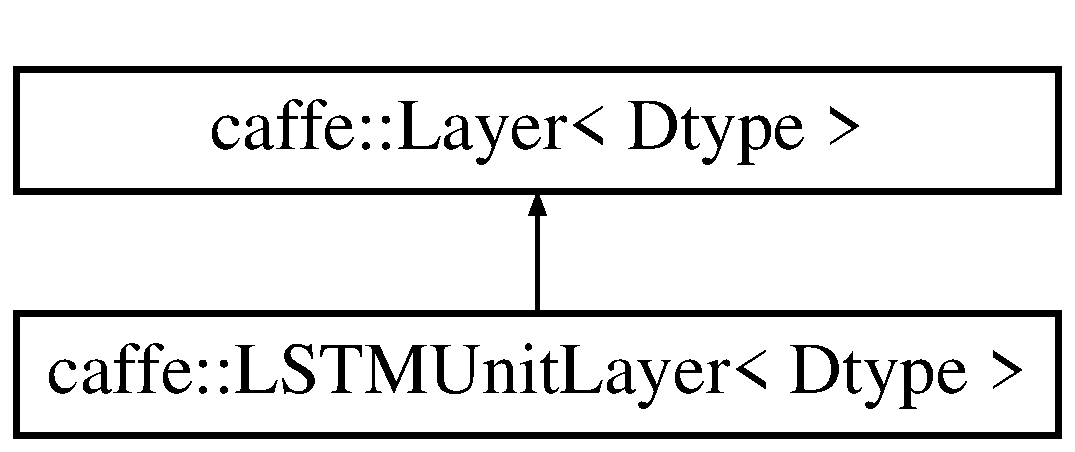
\includegraphics[height=2.000000cm]{classcaffe_1_1LSTMUnitLayer}
\end{center}
\end{figure}
\subsection*{Public Member Functions}
\begin{DoxyCompactItemize}
\item 
{\bfseries L\+S\+T\+M\+Unit\+Layer} (const Layer\+Parameter \&param)\hypertarget{classcaffe_1_1LSTMUnitLayer_aa8eb86f949a93c724c6ed89a601aa4e0}{}\label{classcaffe_1_1LSTMUnitLayer_aa8eb86f949a93c724c6ed89a601aa4e0}

\item 
virtual void \hyperlink{classcaffe_1_1LSTMUnitLayer_ac968816014ba1a2851df2dd8792da21a}{Reshape} (const vector$<$ \hyperlink{classcaffe_1_1Blob}{Blob}$<$ Dtype $>$ $\ast$ $>$ \&bottom, const vector$<$ \hyperlink{classcaffe_1_1Blob}{Blob}$<$ Dtype $>$ $\ast$ $>$ \&top)
\begin{DoxyCompactList}\small\item\em Adjust the shapes of top blobs and internal buffers to accommodate the shapes of the bottom blobs. \end{DoxyCompactList}\item 
virtual const char $\ast$ \hyperlink{classcaffe_1_1LSTMUnitLayer_a6408d25bcd3046db18c1a7b199955886}{type} () const \hypertarget{classcaffe_1_1LSTMUnitLayer_a6408d25bcd3046db18c1a7b199955886}{}\label{classcaffe_1_1LSTMUnitLayer_a6408d25bcd3046db18c1a7b199955886}

\begin{DoxyCompactList}\small\item\em Returns the layer type. \end{DoxyCompactList}\item 
virtual int \hyperlink{classcaffe_1_1LSTMUnitLayer_a865a9e9d8b1d24cd46cabcec81169b01}{Exact\+Num\+Bottom\+Blobs} () const 
\begin{DoxyCompactList}\small\item\em Returns the exact number of bottom blobs required by the layer, or -\/1 if no exact number is required. \end{DoxyCompactList}\item 
virtual int \hyperlink{classcaffe_1_1LSTMUnitLayer_a6e547d63245347dac2aa412281d93970}{Exact\+Num\+Top\+Blobs} () const 
\begin{DoxyCompactList}\small\item\em Returns the exact number of top blobs required by the layer, or -\/1 if no exact number is required. \end{DoxyCompactList}\item 
virtual bool \hyperlink{classcaffe_1_1LSTMUnitLayer_a28bbfffaf2a438f151566c7e53bbc1d7}{Allow\+Force\+Backward} (const int bottom\+\_\+index) const 
\begin{DoxyCompactList}\small\item\em Return whether to allow force\+\_\+backward for a given bottom blob index. \end{DoxyCompactList}\end{DoxyCompactItemize}
\subsection*{Protected Member Functions}
\begin{DoxyCompactItemize}
\item 
virtual void \hyperlink{classcaffe_1_1LSTMUnitLayer_a298ab31f0efac45ee4d0e90448e1b6aa}{Forward\+\_\+cpu} (const vector$<$ \hyperlink{classcaffe_1_1Blob}{Blob}$<$ Dtype $>$ $\ast$ $>$ \&bottom, const vector$<$ \hyperlink{classcaffe_1_1Blob}{Blob}$<$ Dtype $>$ $\ast$ $>$ \&top)
\item 
virtual void \hyperlink{classcaffe_1_1LSTMUnitLayer_adc6533e64de0eec9943ef473f91fb666}{Forward\+\_\+gpu} (const vector$<$ \hyperlink{classcaffe_1_1Blob}{Blob}$<$ Dtype $>$ $\ast$ $>$ \&bottom, const vector$<$ \hyperlink{classcaffe_1_1Blob}{Blob}$<$ Dtype $>$ $\ast$ $>$ \&top)\hypertarget{classcaffe_1_1LSTMUnitLayer_adc6533e64de0eec9943ef473f91fb666}{}\label{classcaffe_1_1LSTMUnitLayer_adc6533e64de0eec9943ef473f91fb666}

\begin{DoxyCompactList}\small\item\em Using the G\+PU device, compute the layer output. Fall back to \hyperlink{classcaffe_1_1LSTMUnitLayer_a298ab31f0efac45ee4d0e90448e1b6aa}{Forward\+\_\+cpu()} if unavailable. \end{DoxyCompactList}\item 
virtual void \hyperlink{classcaffe_1_1LSTMUnitLayer_ab93442722c012f0270e15b3b3ea30cf5}{Backward\+\_\+cpu} (const vector$<$ \hyperlink{classcaffe_1_1Blob}{Blob}$<$ Dtype $>$ $\ast$ $>$ \&top, const vector$<$ bool $>$ \&propagate\+\_\+down, const vector$<$ \hyperlink{classcaffe_1_1Blob}{Blob}$<$ Dtype $>$ $\ast$ $>$ \&bottom)
\begin{DoxyCompactList}\small\item\em Computes the error gradient w.\+r.\+t. the L\+S\+T\+M\+Unit inputs. \end{DoxyCompactList}\item 
virtual void \hyperlink{classcaffe_1_1LSTMUnitLayer_a65a777f73b1b4e3d007a7e2309b3f36e}{Backward\+\_\+gpu} (const vector$<$ \hyperlink{classcaffe_1_1Blob}{Blob}$<$ Dtype $>$ $\ast$ $>$ \&top, const vector$<$ bool $>$ \&propagate\+\_\+down, const vector$<$ \hyperlink{classcaffe_1_1Blob}{Blob}$<$ Dtype $>$ $\ast$ $>$ \&bottom)\hypertarget{classcaffe_1_1LSTMUnitLayer_a65a777f73b1b4e3d007a7e2309b3f36e}{}\label{classcaffe_1_1LSTMUnitLayer_a65a777f73b1b4e3d007a7e2309b3f36e}

\begin{DoxyCompactList}\small\item\em Using the G\+PU device, compute the gradients for any parameters and for the bottom blobs if propagate\+\_\+down is true. Fall back to \hyperlink{classcaffe_1_1LSTMUnitLayer_ab93442722c012f0270e15b3b3ea30cf5}{Backward\+\_\+cpu()} if unavailable. \end{DoxyCompactList}\end{DoxyCompactItemize}
\subsection*{Protected Attributes}
\begin{DoxyCompactItemize}
\item 
int \hyperlink{classcaffe_1_1LSTMUnitLayer_a7ffcad2a4e6ca83f03cc88dffa32b7ca}{hidden\+\_\+dim\+\_\+}\hypertarget{classcaffe_1_1LSTMUnitLayer_a7ffcad2a4e6ca83f03cc88dffa32b7ca}{}\label{classcaffe_1_1LSTMUnitLayer_a7ffcad2a4e6ca83f03cc88dffa32b7ca}

\begin{DoxyCompactList}\small\item\em The hidden and output dimension. \end{DoxyCompactList}\item 
\hyperlink{classcaffe_1_1Blob}{Blob}$<$ Dtype $>$ {\bfseries X\+\_\+acts\+\_\+}\hypertarget{classcaffe_1_1LSTMUnitLayer_a136b722511c1dd446b8ec2298439d805}{}\label{classcaffe_1_1LSTMUnitLayer_a136b722511c1dd446b8ec2298439d805}

\end{DoxyCompactItemize}


\subsection{Detailed Description}
\subsubsection*{template$<$typename Dtype$>$\\*
class caffe\+::\+L\+S\+T\+M\+Unit\+Layer$<$ Dtype $>$}

A helper for \hyperlink{classcaffe_1_1LSTMLayer}{L\+S\+T\+M\+Layer}\+: computes a single timestep of the non-\/linearity of the L\+S\+TM, producing the updated cell and hidden states. 

\subsection{Member Function Documentation}
\index{caffe\+::\+L\+S\+T\+M\+Unit\+Layer@{caffe\+::\+L\+S\+T\+M\+Unit\+Layer}!Allow\+Force\+Backward@{Allow\+Force\+Backward}}
\index{Allow\+Force\+Backward@{Allow\+Force\+Backward}!caffe\+::\+L\+S\+T\+M\+Unit\+Layer@{caffe\+::\+L\+S\+T\+M\+Unit\+Layer}}
\subsubsection[{\texorpdfstring{Allow\+Force\+Backward(const int bottom\+\_\+index) const }{AllowForceBackward(const int bottom_index) const }}]{\setlength{\rightskip}{0pt plus 5cm}template$<$typename Dtype $>$ virtual bool {\bf caffe\+::\+L\+S\+T\+M\+Unit\+Layer}$<$ Dtype $>$\+::Allow\+Force\+Backward (
\begin{DoxyParamCaption}
\item[{const int}]{bottom\+\_\+index}
\end{DoxyParamCaption}
) const\hspace{0.3cm}{\ttfamily [inline]}, {\ttfamily [virtual]}}\hypertarget{classcaffe_1_1LSTMUnitLayer_a28bbfffaf2a438f151566c7e53bbc1d7}{}\label{classcaffe_1_1LSTMUnitLayer_a28bbfffaf2a438f151566c7e53bbc1d7}


Return whether to allow force\+\_\+backward for a given bottom blob index. 

If Allow\+Force\+Backward(i) == false, we will ignore the force\+\_\+backward setting and backpropagate to blob i only if it needs gradient information (as is done when force\+\_\+backward == false). 

Reimplemented from \hyperlink{classcaffe_1_1Layer_a4a2e4ca94eaa1cbc054b512c6657743e}{caffe\+::\+Layer$<$ Dtype $>$}.

\index{caffe\+::\+L\+S\+T\+M\+Unit\+Layer@{caffe\+::\+L\+S\+T\+M\+Unit\+Layer}!Backward\+\_\+cpu@{Backward\+\_\+cpu}}
\index{Backward\+\_\+cpu@{Backward\+\_\+cpu}!caffe\+::\+L\+S\+T\+M\+Unit\+Layer@{caffe\+::\+L\+S\+T\+M\+Unit\+Layer}}
\subsubsection[{\texorpdfstring{Backward\+\_\+cpu(const vector$<$ Blob$<$ Dtype $>$ $\ast$ $>$ \&top, const vector$<$ bool $>$ \&propagate\+\_\+down, const vector$<$ Blob$<$ Dtype $>$ $\ast$ $>$ \&bottom)}{Backward_cpu(const vector< Blob< Dtype > * > &top, const vector< bool > &propagate_down, const vector< Blob< Dtype > * > &bottom)}}]{\setlength{\rightskip}{0pt plus 5cm}template$<$typename Dtype $>$ void {\bf caffe\+::\+L\+S\+T\+M\+Unit\+Layer}$<$ Dtype $>$\+::Backward\+\_\+cpu (
\begin{DoxyParamCaption}
\item[{const vector$<$ {\bf Blob}$<$ Dtype $>$ $\ast$ $>$ \&}]{top, }
\item[{const vector$<$ bool $>$ \&}]{propagate\+\_\+down, }
\item[{const vector$<$ {\bf Blob}$<$ Dtype $>$ $\ast$ $>$ \&}]{bottom}
\end{DoxyParamCaption}
)\hspace{0.3cm}{\ttfamily [protected]}, {\ttfamily [virtual]}}\hypertarget{classcaffe_1_1LSTMUnitLayer_ab93442722c012f0270e15b3b3ea30cf5}{}\label{classcaffe_1_1LSTMUnitLayer_ab93442722c012f0270e15b3b3ea30cf5}


Computes the error gradient w.\+r.\+t. the L\+S\+T\+M\+Unit inputs. 


\begin{DoxyParams}{Parameters}
{\em top} & output \hyperlink{classcaffe_1_1Blob}{Blob} vector (length 2), providing the error gradient with respect to the outputs
\begin{DoxyEnumerate}
\item $ (1 \times N \times D) $\+: containing error gradients $ \frac{\partial E}{\partial c_t} $ with respect to the updated cell state $ c_t $
\item $ (1 \times N \times D) $\+: containing error gradients $ \frac{\partial E}{\partial h_t} $ with respect to the updated cell state $ h_t $ 
\end{DoxyEnumerate}\\
\hline
{\em propagate\+\_\+down} & see \hyperlink{classcaffe_1_1Layer_a53df1e081767e07bfb4c81657f4acd0a}{Layer\+::\+Backward}. \\
\hline
{\em bottom} & input \hyperlink{classcaffe_1_1Blob}{Blob} vector (length 3), into which the error gradients with respect to the L\+S\+T\+M\+Unit inputs $ c_{t-1} $ and the gate inputs are computed. Computatation of the error gradients w.\+r.\+t. the sequence indicators is not implemented.
\begin{DoxyEnumerate}
\item $ (1 \times N \times D) $ the error gradient w.\+r.\+t. the previous timestep cell state $ c_{t-1} $
\item $ (1 \times N \times 4D) $ the error gradient w.\+r.\+t. the \char`\"{}gate inputs\char`\"{} $ [ \frac{\partial E}{\partial i_t} \frac{\partial E}{\partial f_t} \frac{\partial E}{\partial o_t} \frac{\partial E}{\partial g_t} ] $
\item $ (1 \times 1 \times N) $ the gradient w.\+r.\+t. the sequence continuation indicators $ \delta_t $ is currently not computed. 
\end{DoxyEnumerate}\\
\hline
\end{DoxyParams}


Implements \hyperlink{classcaffe_1_1Layer_a64d15855f882af4b82e83fa993c4e7c6}{caffe\+::\+Layer$<$ Dtype $>$}.

\index{caffe\+::\+L\+S\+T\+M\+Unit\+Layer@{caffe\+::\+L\+S\+T\+M\+Unit\+Layer}!Exact\+Num\+Bottom\+Blobs@{Exact\+Num\+Bottom\+Blobs}}
\index{Exact\+Num\+Bottom\+Blobs@{Exact\+Num\+Bottom\+Blobs}!caffe\+::\+L\+S\+T\+M\+Unit\+Layer@{caffe\+::\+L\+S\+T\+M\+Unit\+Layer}}
\subsubsection[{\texorpdfstring{Exact\+Num\+Bottom\+Blobs() const }{ExactNumBottomBlobs() const }}]{\setlength{\rightskip}{0pt plus 5cm}template$<$typename Dtype $>$ virtual int {\bf caffe\+::\+L\+S\+T\+M\+Unit\+Layer}$<$ Dtype $>$\+::Exact\+Num\+Bottom\+Blobs (
\begin{DoxyParamCaption}
{}
\end{DoxyParamCaption}
) const\hspace{0.3cm}{\ttfamily [inline]}, {\ttfamily [virtual]}}\hypertarget{classcaffe_1_1LSTMUnitLayer_a865a9e9d8b1d24cd46cabcec81169b01}{}\label{classcaffe_1_1LSTMUnitLayer_a865a9e9d8b1d24cd46cabcec81169b01}


Returns the exact number of bottom blobs required by the layer, or -\/1 if no exact number is required. 

This method should be overridden to return a non-\/negative value if your layer expects some exact number of bottom blobs. 

Reimplemented from \hyperlink{classcaffe_1_1Layer_a45c7a7943a8a6735ac433c9be11e0240}{caffe\+::\+Layer$<$ Dtype $>$}.

\index{caffe\+::\+L\+S\+T\+M\+Unit\+Layer@{caffe\+::\+L\+S\+T\+M\+Unit\+Layer}!Exact\+Num\+Top\+Blobs@{Exact\+Num\+Top\+Blobs}}
\index{Exact\+Num\+Top\+Blobs@{Exact\+Num\+Top\+Blobs}!caffe\+::\+L\+S\+T\+M\+Unit\+Layer@{caffe\+::\+L\+S\+T\+M\+Unit\+Layer}}
\subsubsection[{\texorpdfstring{Exact\+Num\+Top\+Blobs() const }{ExactNumTopBlobs() const }}]{\setlength{\rightskip}{0pt plus 5cm}template$<$typename Dtype $>$ virtual int {\bf caffe\+::\+L\+S\+T\+M\+Unit\+Layer}$<$ Dtype $>$\+::Exact\+Num\+Top\+Blobs (
\begin{DoxyParamCaption}
{}
\end{DoxyParamCaption}
) const\hspace{0.3cm}{\ttfamily [inline]}, {\ttfamily [virtual]}}\hypertarget{classcaffe_1_1LSTMUnitLayer_a6e547d63245347dac2aa412281d93970}{}\label{classcaffe_1_1LSTMUnitLayer_a6e547d63245347dac2aa412281d93970}


Returns the exact number of top blobs required by the layer, or -\/1 if no exact number is required. 

This method should be overridden to return a non-\/negative value if your layer expects some exact number of top blobs. 

Reimplemented from \hyperlink{classcaffe_1_1Layer_aa3c99ed707e8db683a3043412e151af8}{caffe\+::\+Layer$<$ Dtype $>$}.

\index{caffe\+::\+L\+S\+T\+M\+Unit\+Layer@{caffe\+::\+L\+S\+T\+M\+Unit\+Layer}!Forward\+\_\+cpu@{Forward\+\_\+cpu}}
\index{Forward\+\_\+cpu@{Forward\+\_\+cpu}!caffe\+::\+L\+S\+T\+M\+Unit\+Layer@{caffe\+::\+L\+S\+T\+M\+Unit\+Layer}}
\subsubsection[{\texorpdfstring{Forward\+\_\+cpu(const vector$<$ Blob$<$ Dtype $>$ $\ast$ $>$ \&bottom, const vector$<$ Blob$<$ Dtype $>$ $\ast$ $>$ \&top)}{Forward_cpu(const vector< Blob< Dtype > * > &bottom, const vector< Blob< Dtype > * > &top)}}]{\setlength{\rightskip}{0pt plus 5cm}template$<$typename Dtype $>$ void {\bf caffe\+::\+L\+S\+T\+M\+Unit\+Layer}$<$ Dtype $>$\+::Forward\+\_\+cpu (
\begin{DoxyParamCaption}
\item[{const vector$<$ {\bf Blob}$<$ Dtype $>$ $\ast$ $>$ \&}]{bottom, }
\item[{const vector$<$ {\bf Blob}$<$ Dtype $>$ $\ast$ $>$ \&}]{top}
\end{DoxyParamCaption}
)\hspace{0.3cm}{\ttfamily [protected]}, {\ttfamily [virtual]}}\hypertarget{classcaffe_1_1LSTMUnitLayer_a298ab31f0efac45ee4d0e90448e1b6aa}{}\label{classcaffe_1_1LSTMUnitLayer_a298ab31f0efac45ee4d0e90448e1b6aa}

\begin{DoxyParams}{Parameters}
{\em bottom} & input \hyperlink{classcaffe_1_1Blob}{Blob} vector (length 3)
\begin{DoxyEnumerate}
\item $ (1 \times N \times D) $ the previous timestep cell state $ c_{t-1} $
\item $ (1 \times N \times 4D) $ the \char`\"{}gate inputs\char`\"{} $ [i_t', f_t', o_t', g_t'] $
\item $ (1 \times N) $ the sequence continuation indicators $ \delta_t $ 
\end{DoxyEnumerate}\\
\hline
{\em top} & output \hyperlink{classcaffe_1_1Blob}{Blob} vector (length 2)
\begin{DoxyEnumerate}
\item $ (1 \times N \times D) $ the updated cell state $ c_t $, computed as\+: i\+\_\+t \+:= \mbox{[}i\+\_\+t\textquotesingle{}\mbox{]} f\+\_\+t \+:= \mbox{[}f\+\_\+t\textquotesingle{}\mbox{]} o\+\_\+t \+:= \mbox{[}o\+\_\+t\textquotesingle{}\mbox{]} g\+\_\+t \+:= \mbox{[}g\+\_\+t\textquotesingle{}\mbox{]} c\+\_\+t \+:= cont\+\_\+t $\ast$ (f\+\_\+t .$\ast$ c\+\_\+\{t-\/1\}) + (i\+\_\+t .$\ast$ g\+\_\+t)
\item $ (1 \times N \times D) $ the updated hidden state $ h_t $, computed as\+: h\+\_\+t \+:= o\+\_\+t .$\ast$ \mbox{[}c\+\_\+t\mbox{]} 
\end{DoxyEnumerate}\\
\hline
\end{DoxyParams}


Implements \hyperlink{classcaffe_1_1Layer_add965883f75bbf90c7a06f960cda7a1a}{caffe\+::\+Layer$<$ Dtype $>$}.

\index{caffe\+::\+L\+S\+T\+M\+Unit\+Layer@{caffe\+::\+L\+S\+T\+M\+Unit\+Layer}!Reshape@{Reshape}}
\index{Reshape@{Reshape}!caffe\+::\+L\+S\+T\+M\+Unit\+Layer@{caffe\+::\+L\+S\+T\+M\+Unit\+Layer}}
\subsubsection[{\texorpdfstring{Reshape(const vector$<$ Blob$<$ Dtype $>$ $\ast$ $>$ \&bottom, const vector$<$ Blob$<$ Dtype $>$ $\ast$ $>$ \&top)}{Reshape(const vector< Blob< Dtype > * > &bottom, const vector< Blob< Dtype > * > &top)}}]{\setlength{\rightskip}{0pt plus 5cm}template$<$typename Dtype $>$ void {\bf caffe\+::\+L\+S\+T\+M\+Unit\+Layer}$<$ Dtype $>$\+::Reshape (
\begin{DoxyParamCaption}
\item[{const vector$<$ {\bf Blob}$<$ Dtype $>$ $\ast$ $>$ \&}]{bottom, }
\item[{const vector$<$ {\bf Blob}$<$ Dtype $>$ $\ast$ $>$ \&}]{top}
\end{DoxyParamCaption}
)\hspace{0.3cm}{\ttfamily [virtual]}}\hypertarget{classcaffe_1_1LSTMUnitLayer_ac968816014ba1a2851df2dd8792da21a}{}\label{classcaffe_1_1LSTMUnitLayer_ac968816014ba1a2851df2dd8792da21a}


Adjust the shapes of top blobs and internal buffers to accommodate the shapes of the bottom blobs. 


\begin{DoxyParams}{Parameters}
{\em bottom} & the input blobs, with the requested input shapes \\
\hline
{\em top} & the top blobs, which should be reshaped as needed\\
\hline
\end{DoxyParams}
This method should reshape top blobs as needed according to the shapes of the bottom (input) blobs, as well as reshaping any internal buffers and making any other necessary adjustments so that the layer can accommodate the bottom blobs. 

Implements \hyperlink{classcaffe_1_1Layer_ad9d391b972c769c0ebee34ca6d1c973e}{caffe\+::\+Layer$<$ Dtype $>$}.



The documentation for this class was generated from the following files\+:\begin{DoxyCompactItemize}
\item 
include/caffe/layers/lstm\+\_\+layer.\+hpp\item 
src/caffe/layers/lstm\+\_\+unit\+\_\+layer.\+cpp\end{DoxyCompactItemize}

\hypertarget{classcaffe_1_1MemoryDataLayer}{}\section{caffe\+:\+:Memory\+Data\+Layer$<$ Dtype $>$ Class Template Reference}
\label{classcaffe_1_1MemoryDataLayer}\index{caffe\+::\+Memory\+Data\+Layer$<$ Dtype $>$@{caffe\+::\+Memory\+Data\+Layer$<$ Dtype $>$}}


Provides data to the \hyperlink{classcaffe_1_1Net}{Net} from memory.  




{\ttfamily \#include $<$memory\+\_\+data\+\_\+layer.\+hpp$>$}

Inheritance diagram for caffe\+:\+:Memory\+Data\+Layer$<$ Dtype $>$\+:\begin{figure}[H]
\begin{center}
\leavevmode
\includegraphics[height=3.000000cm]{classcaffe_1_1MemoryDataLayer}
\end{center}
\end{figure}
\subsection*{Public Member Functions}
\begin{DoxyCompactItemize}
\item 
{\bfseries Memory\+Data\+Layer} (const Layer\+Parameter \&param)\hypertarget{classcaffe_1_1MemoryDataLayer_a9bf012786068bfe846694af129a6736f}{}\label{classcaffe_1_1MemoryDataLayer_a9bf012786068bfe846694af129a6736f}

\item 
virtual void {\bfseries Data\+Layer\+Set\+Up} (const vector$<$ \hyperlink{classcaffe_1_1Blob}{Blob}$<$ Dtype $>$ $\ast$ $>$ \&bottom, const vector$<$ \hyperlink{classcaffe_1_1Blob}{Blob}$<$ Dtype $>$ $\ast$ $>$ \&top)\hypertarget{classcaffe_1_1MemoryDataLayer_a34d6d4a496648d6209999f6004df08e3}{}\label{classcaffe_1_1MemoryDataLayer_a34d6d4a496648d6209999f6004df08e3}

\item 
virtual const char $\ast$ \hyperlink{classcaffe_1_1MemoryDataLayer_a52298f383fa52ccf0c61e54f46ba9cda}{type} () const \hypertarget{classcaffe_1_1MemoryDataLayer_a52298f383fa52ccf0c61e54f46ba9cda}{}\label{classcaffe_1_1MemoryDataLayer_a52298f383fa52ccf0c61e54f46ba9cda}

\begin{DoxyCompactList}\small\item\em Returns the layer type. \end{DoxyCompactList}\item 
virtual int \hyperlink{classcaffe_1_1MemoryDataLayer_a46529bcce2bf8b8f3984286ad675cbd6}{Exact\+Num\+Bottom\+Blobs} () const 
\begin{DoxyCompactList}\small\item\em Returns the exact number of bottom blobs required by the layer, or -\/1 if no exact number is required. \end{DoxyCompactList}\item 
virtual int \hyperlink{classcaffe_1_1MemoryDataLayer_a973a58b5967809488f0e88c0a9a6fbac}{Exact\+Num\+Top\+Blobs} () const 
\begin{DoxyCompactList}\small\item\em Returns the exact number of top blobs required by the layer, or -\/1 if no exact number is required. \end{DoxyCompactList}\item 
virtual void {\bfseries Add\+Datum\+Vector} (const vector$<$ Datum $>$ \&datum\+\_\+vector)\hypertarget{classcaffe_1_1MemoryDataLayer_a5d7c633d066570d2b040ccabda9d9f60}{}\label{classcaffe_1_1MemoryDataLayer_a5d7c633d066570d2b040ccabda9d9f60}

\item 
void {\bfseries Reset} (Dtype $\ast$data, Dtype $\ast$label, int n)\hypertarget{classcaffe_1_1MemoryDataLayer_aeaa745c4fe3a957b973bf94dca6a5f2b}{}\label{classcaffe_1_1MemoryDataLayer_aeaa745c4fe3a957b973bf94dca6a5f2b}

\item 
void {\bfseries set\+\_\+batch\+\_\+size} (int new\+\_\+size)\hypertarget{classcaffe_1_1MemoryDataLayer_a07bc96b979032d11a0bf00fad6a3f1ff}{}\label{classcaffe_1_1MemoryDataLayer_a07bc96b979032d11a0bf00fad6a3f1ff}

\item 
int {\bfseries batch\+\_\+size} ()\hypertarget{classcaffe_1_1MemoryDataLayer_a06bfb6d06f61db11699a6b3ce7b1ee53}{}\label{classcaffe_1_1MemoryDataLayer_a06bfb6d06f61db11699a6b3ce7b1ee53}

\item 
int {\bfseries channels} ()\hypertarget{classcaffe_1_1MemoryDataLayer_aeeed090aee729e61426525c6a62f79a2}{}\label{classcaffe_1_1MemoryDataLayer_aeeed090aee729e61426525c6a62f79a2}

\item 
int {\bfseries height} ()\hypertarget{classcaffe_1_1MemoryDataLayer_a13775655bc0563ec85f124604ebb945f}{}\label{classcaffe_1_1MemoryDataLayer_a13775655bc0563ec85f124604ebb945f}

\item 
int {\bfseries width} ()\hypertarget{classcaffe_1_1MemoryDataLayer_a2c8b2f60895130d3ebfdc775724b5503}{}\label{classcaffe_1_1MemoryDataLayer_a2c8b2f60895130d3ebfdc775724b5503}

\end{DoxyCompactItemize}
\subsection*{Protected Member Functions}
\begin{DoxyCompactItemize}
\item 
virtual void \hyperlink{classcaffe_1_1MemoryDataLayer_a375e09cfb9898bf5e99f56d3316d0ded}{Forward\+\_\+cpu} (const vector$<$ \hyperlink{classcaffe_1_1Blob}{Blob}$<$ Dtype $>$ $\ast$ $>$ \&bottom, const vector$<$ \hyperlink{classcaffe_1_1Blob}{Blob}$<$ Dtype $>$ $\ast$ $>$ \&top)\hypertarget{classcaffe_1_1MemoryDataLayer_a375e09cfb9898bf5e99f56d3316d0ded}{}\label{classcaffe_1_1MemoryDataLayer_a375e09cfb9898bf5e99f56d3316d0ded}

\begin{DoxyCompactList}\small\item\em Using the C\+PU device, compute the layer output. \end{DoxyCompactList}\end{DoxyCompactItemize}
\subsection*{Protected Attributes}
\begin{DoxyCompactItemize}
\item 
int {\bfseries batch\+\_\+size\+\_\+}\hypertarget{classcaffe_1_1MemoryDataLayer_a94335b05660c950a4ba711342daff276}{}\label{classcaffe_1_1MemoryDataLayer_a94335b05660c950a4ba711342daff276}

\item 
int {\bfseries channels\+\_\+}\hypertarget{classcaffe_1_1MemoryDataLayer_af42ca28f0d1768bdfc679347c3812643}{}\label{classcaffe_1_1MemoryDataLayer_af42ca28f0d1768bdfc679347c3812643}

\item 
int {\bfseries height\+\_\+}\hypertarget{classcaffe_1_1MemoryDataLayer_a815208a6cb35c6712d43ff8b32bcecb9}{}\label{classcaffe_1_1MemoryDataLayer_a815208a6cb35c6712d43ff8b32bcecb9}

\item 
int {\bfseries width\+\_\+}\hypertarget{classcaffe_1_1MemoryDataLayer_afd655a82e4016d543366d694720a786a}{}\label{classcaffe_1_1MemoryDataLayer_afd655a82e4016d543366d694720a786a}

\item 
int {\bfseries size\+\_\+}\hypertarget{classcaffe_1_1MemoryDataLayer_a9c083d81e848814b5f47c950a4d64df8}{}\label{classcaffe_1_1MemoryDataLayer_a9c083d81e848814b5f47c950a4d64df8}

\item 
Dtype $\ast$ {\bfseries data\+\_\+}\hypertarget{classcaffe_1_1MemoryDataLayer_a57a7e3dca84db2b07cb009a44c6ae45c}{}\label{classcaffe_1_1MemoryDataLayer_a57a7e3dca84db2b07cb009a44c6ae45c}

\item 
Dtype $\ast$ {\bfseries labels\+\_\+}\hypertarget{classcaffe_1_1MemoryDataLayer_abf7f9a81ae3268a6eea7fbd97760e28a}{}\label{classcaffe_1_1MemoryDataLayer_abf7f9a81ae3268a6eea7fbd97760e28a}

\item 
int {\bfseries n\+\_\+}\hypertarget{classcaffe_1_1MemoryDataLayer_a303b19a435878a94ede0c8e1fb26f2a1}{}\label{classcaffe_1_1MemoryDataLayer_a303b19a435878a94ede0c8e1fb26f2a1}

\item 
size\+\_\+t {\bfseries pos\+\_\+}\hypertarget{classcaffe_1_1MemoryDataLayer_a6a4867d3666f144f6fdd804a186d789c}{}\label{classcaffe_1_1MemoryDataLayer_a6a4867d3666f144f6fdd804a186d789c}

\item 
\hyperlink{classcaffe_1_1Blob}{Blob}$<$ Dtype $>$ {\bfseries added\+\_\+data\+\_\+}\hypertarget{classcaffe_1_1MemoryDataLayer_ad8b46dabbb7ca61ae58136d40531dcb8}{}\label{classcaffe_1_1MemoryDataLayer_ad8b46dabbb7ca61ae58136d40531dcb8}

\item 
\hyperlink{classcaffe_1_1Blob}{Blob}$<$ Dtype $>$ {\bfseries added\+\_\+label\+\_\+}\hypertarget{classcaffe_1_1MemoryDataLayer_a504d7d75c9e23175dbfbfe8a8a788b4d}{}\label{classcaffe_1_1MemoryDataLayer_a504d7d75c9e23175dbfbfe8a8a788b4d}

\item 
bool {\bfseries has\+\_\+new\+\_\+data\+\_\+}\hypertarget{classcaffe_1_1MemoryDataLayer_a853f5cc1091152cac0ef6cbf57ac253a}{}\label{classcaffe_1_1MemoryDataLayer_a853f5cc1091152cac0ef6cbf57ac253a}

\end{DoxyCompactItemize}


\subsection{Detailed Description}
\subsubsection*{template$<$typename Dtype$>$\\*
class caffe\+::\+Memory\+Data\+Layer$<$ Dtype $>$}

Provides data to the \hyperlink{classcaffe_1_1Net}{Net} from memory. 

T\+O\+D\+O(dox)\+: thorough documentation for Forward and proto params. 

\subsection{Member Function Documentation}
\index{caffe\+::\+Memory\+Data\+Layer@{caffe\+::\+Memory\+Data\+Layer}!Exact\+Num\+Bottom\+Blobs@{Exact\+Num\+Bottom\+Blobs}}
\index{Exact\+Num\+Bottom\+Blobs@{Exact\+Num\+Bottom\+Blobs}!caffe\+::\+Memory\+Data\+Layer@{caffe\+::\+Memory\+Data\+Layer}}
\subsubsection[{\texorpdfstring{Exact\+Num\+Bottom\+Blobs() const }{ExactNumBottomBlobs() const }}]{\setlength{\rightskip}{0pt plus 5cm}template$<$typename Dtype $>$ virtual int {\bf caffe\+::\+Memory\+Data\+Layer}$<$ Dtype $>$\+::Exact\+Num\+Bottom\+Blobs (
\begin{DoxyParamCaption}
{}
\end{DoxyParamCaption}
) const\hspace{0.3cm}{\ttfamily [inline]}, {\ttfamily [virtual]}}\hypertarget{classcaffe_1_1MemoryDataLayer_a46529bcce2bf8b8f3984286ad675cbd6}{}\label{classcaffe_1_1MemoryDataLayer_a46529bcce2bf8b8f3984286ad675cbd6}


Returns the exact number of bottom blobs required by the layer, or -\/1 if no exact number is required. 

This method should be overridden to return a non-\/negative value if your layer expects some exact number of bottom blobs. 

Reimplemented from \hyperlink{classcaffe_1_1Layer_a45c7a7943a8a6735ac433c9be11e0240}{caffe\+::\+Layer$<$ Dtype $>$}.

\index{caffe\+::\+Memory\+Data\+Layer@{caffe\+::\+Memory\+Data\+Layer}!Exact\+Num\+Top\+Blobs@{Exact\+Num\+Top\+Blobs}}
\index{Exact\+Num\+Top\+Blobs@{Exact\+Num\+Top\+Blobs}!caffe\+::\+Memory\+Data\+Layer@{caffe\+::\+Memory\+Data\+Layer}}
\subsubsection[{\texorpdfstring{Exact\+Num\+Top\+Blobs() const }{ExactNumTopBlobs() const }}]{\setlength{\rightskip}{0pt plus 5cm}template$<$typename Dtype $>$ virtual int {\bf caffe\+::\+Memory\+Data\+Layer}$<$ Dtype $>$\+::Exact\+Num\+Top\+Blobs (
\begin{DoxyParamCaption}
{}
\end{DoxyParamCaption}
) const\hspace{0.3cm}{\ttfamily [inline]}, {\ttfamily [virtual]}}\hypertarget{classcaffe_1_1MemoryDataLayer_a973a58b5967809488f0e88c0a9a6fbac}{}\label{classcaffe_1_1MemoryDataLayer_a973a58b5967809488f0e88c0a9a6fbac}


Returns the exact number of top blobs required by the layer, or -\/1 if no exact number is required. 

This method should be overridden to return a non-\/negative value if your layer expects some exact number of top blobs. 

Reimplemented from \hyperlink{classcaffe_1_1Layer_aa3c99ed707e8db683a3043412e151af8}{caffe\+::\+Layer$<$ Dtype $>$}.



The documentation for this class was generated from the following files\+:\begin{DoxyCompactItemize}
\item 
include/caffe/layers/memory\+\_\+data\+\_\+layer.\+hpp\item 
src/caffe/layers/memory\+\_\+data\+\_\+layer.\+cpp\end{DoxyCompactItemize}

\hypertarget{classcaffe_1_1MSRAFiller}{}\section{caffe\+:\+:M\+S\+R\+A\+Filler$<$ Dtype $>$ Class Template Reference}
\label{classcaffe_1_1MSRAFiller}\index{caffe\+::\+M\+S\+R\+A\+Filler$<$ Dtype $>$@{caffe\+::\+M\+S\+R\+A\+Filler$<$ Dtype $>$}}


Fills a \hyperlink{classcaffe_1_1Blob}{Blob} with values $ x \sim N(0, \sigma^2) $ where $ \sigma^2 $ is set inversely proportional to number of incoming nodes, outgoing nodes, or their average.  




{\ttfamily \#include $<$filler.\+hpp$>$}

Inheritance diagram for caffe\+:\+:M\+S\+R\+A\+Filler$<$ Dtype $>$\+:\begin{figure}[H]
\begin{center}
\leavevmode
\includegraphics[height=2.000000cm]{classcaffe_1_1MSRAFiller}
\end{center}
\end{figure}
\subsection*{Public Member Functions}
\begin{DoxyCompactItemize}
\item 
{\bfseries M\+S\+R\+A\+Filler} (const Filler\+Parameter \&param)\hypertarget{classcaffe_1_1MSRAFiller_a68b0367c462b9cfce5379074105282c9}{}\label{classcaffe_1_1MSRAFiller_a68b0367c462b9cfce5379074105282c9}

\item 
virtual void {\bfseries Fill} (\hyperlink{classcaffe_1_1Blob}{Blob}$<$ Dtype $>$ $\ast$blob)\hypertarget{classcaffe_1_1MSRAFiller_a174e9fab9be5c0c598680bebc621ab8f}{}\label{classcaffe_1_1MSRAFiller_a174e9fab9be5c0c598680bebc621ab8f}

\end{DoxyCompactItemize}
\subsection*{Additional Inherited Members}


\subsection{Detailed Description}
\subsubsection*{template$<$typename Dtype$>$\\*
class caffe\+::\+M\+S\+R\+A\+Filler$<$ Dtype $>$}

Fills a \hyperlink{classcaffe_1_1Blob}{Blob} with values $ x \sim N(0, \sigma^2) $ where $ \sigma^2 $ is set inversely proportional to number of incoming nodes, outgoing nodes, or their average. 

A \hyperlink{classcaffe_1_1Filler}{Filler} based on the paper \mbox{[}He, Zhang, Ren and Sun 2015\mbox{]}\+: Specifically accounts for Re\+LU nonlinearities.

Aside\+: for another perspective on the scaling factor, see the derivation of \mbox{[}Saxe, Mc\+Clelland, and Ganguli 2013 (v3)\mbox{]}.

It fills the incoming matrix by randomly sampling Gaussian data with std = sqrt(2 / n) where n is the fan\+\_\+in, fan\+\_\+out, or their average, depending on the variance\+\_\+norm option. You should make sure the input blob has shape (num, a, b, c) where a $\ast$ b $\ast$ c = fan\+\_\+in and num $\ast$ b $\ast$ c = fan\+\_\+out. Note that this is currently not the case for inner product layers. 

The documentation for this class was generated from the following file\+:\begin{DoxyCompactItemize}
\item 
include/caffe/filler.\+hpp\end{DoxyCompactItemize}

\hypertarget{classcaffe_1_1MultinomialLogisticLossLayer}{}\section{caffe\+:\+:Multinomial\+Logistic\+Loss\+Layer$<$ Dtype $>$ Class Template Reference}
\label{classcaffe_1_1MultinomialLogisticLossLayer}\index{caffe\+::\+Multinomial\+Logistic\+Loss\+Layer$<$ Dtype $>$@{caffe\+::\+Multinomial\+Logistic\+Loss\+Layer$<$ Dtype $>$}}


Computes the multinomial logistic loss for a one-\/of-\/many classification task, directly taking a predicted probability distribution as input.  




{\ttfamily \#include $<$multinomial\+\_\+logistic\+\_\+loss\+\_\+layer.\+hpp$>$}

Inheritance diagram for caffe\+:\+:Multinomial\+Logistic\+Loss\+Layer$<$ Dtype $>$\+:\begin{figure}[H]
\begin{center}
\leavevmode
\includegraphics[height=3.000000cm]{classcaffe_1_1MultinomialLogisticLossLayer}
\end{center}
\end{figure}
\subsection*{Public Member Functions}
\begin{DoxyCompactItemize}
\item 
{\bfseries Multinomial\+Logistic\+Loss\+Layer} (const Layer\+Parameter \&param)\hypertarget{classcaffe_1_1MultinomialLogisticLossLayer_a1c9567f9901885ec4737cf9315d52081}{}\label{classcaffe_1_1MultinomialLogisticLossLayer_a1c9567f9901885ec4737cf9315d52081}

\item 
virtual void \hyperlink{classcaffe_1_1MultinomialLogisticLossLayer_a906947b9029c3ba8127591c49855ccb6}{Reshape} (const vector$<$ \hyperlink{classcaffe_1_1Blob}{Blob}$<$ Dtype $>$ $\ast$ $>$ \&bottom, const vector$<$ \hyperlink{classcaffe_1_1Blob}{Blob}$<$ Dtype $>$ $\ast$ $>$ \&top)
\begin{DoxyCompactList}\small\item\em Adjust the shapes of top blobs and internal buffers to accommodate the shapes of the bottom blobs. \end{DoxyCompactList}\item 
virtual const char $\ast$ \hyperlink{classcaffe_1_1MultinomialLogisticLossLayer_abae46c53aa81a1517d85d6704f2f71a6}{type} () const \hypertarget{classcaffe_1_1MultinomialLogisticLossLayer_abae46c53aa81a1517d85d6704f2f71a6}{}\label{classcaffe_1_1MultinomialLogisticLossLayer_abae46c53aa81a1517d85d6704f2f71a6}

\begin{DoxyCompactList}\small\item\em Returns the layer type. \end{DoxyCompactList}\end{DoxyCompactItemize}
\subsection*{Protected Member Functions}
\begin{DoxyCompactItemize}
\item 
virtual void \hyperlink{classcaffe_1_1MultinomialLogisticLossLayer_ac1b7b60b9439d9679664783a167a36d6}{Forward\+\_\+cpu} (const vector$<$ \hyperlink{classcaffe_1_1Blob}{Blob}$<$ Dtype $>$ $\ast$ $>$ \&bottom, const vector$<$ \hyperlink{classcaffe_1_1Blob}{Blob}$<$ Dtype $>$ $\ast$ $>$ \&top)
\begin{DoxyCompactList}\small\item\em Computes the multinomial logistic loss for a one-\/of-\/many classification task, directly taking a predicted probability distribution as input. \end{DoxyCompactList}\item 
virtual void \hyperlink{classcaffe_1_1MultinomialLogisticLossLayer_a93b273f7c2180dff92cbc8d4f5ba353d}{Backward\+\_\+cpu} (const vector$<$ \hyperlink{classcaffe_1_1Blob}{Blob}$<$ Dtype $>$ $\ast$ $>$ \&top, const vector$<$ bool $>$ \&propagate\+\_\+down, const vector$<$ \hyperlink{classcaffe_1_1Blob}{Blob}$<$ Dtype $>$ $\ast$ $>$ \&bottom)
\begin{DoxyCompactList}\small\item\em Computes the multinomial logistic loss error gradient w.\+r.\+t. the predictions. \end{DoxyCompactList}\end{DoxyCompactItemize}
\subsection*{Additional Inherited Members}


\subsection{Detailed Description}
\subsubsection*{template$<$typename Dtype$>$\\*
class caffe\+::\+Multinomial\+Logistic\+Loss\+Layer$<$ Dtype $>$}

Computes the multinomial logistic loss for a one-\/of-\/many classification task, directly taking a predicted probability distribution as input. 

When predictions are not already a probability distribution, you should instead use the \hyperlink{classcaffe_1_1SoftmaxWithLossLayer}{Softmax\+With\+Loss\+Layer}, which maps predictions to a distribution using the \hyperlink{classcaffe_1_1SoftmaxLayer}{Softmax\+Layer}, before computing the multinomial logistic loss. The \hyperlink{classcaffe_1_1SoftmaxWithLossLayer}{Softmax\+With\+Loss\+Layer} should be preferred over separate \hyperlink{classcaffe_1_1SoftmaxLayer}{Softmax\+Layer} + \hyperlink{classcaffe_1_1MultinomialLogisticLossLayer}{Multinomial\+Logistic\+Loss\+Layer} as its gradient computation is more numerically stable.


\begin{DoxyParams}{Parameters}
{\em bottom} & input \hyperlink{classcaffe_1_1Blob}{Blob} vector (length 2)
\begin{DoxyEnumerate}
\item $ (N \times C \times H \times W) $ the predictions $ \hat{p} $, a \hyperlink{classcaffe_1_1Blob}{Blob} with values in $ [0, 1] $ indicating the predicted probability of each of the $ K = CHW $ classes. Each prediction vector $ \hat{p}_n $ should sum to 1 as in a probability distribution\+: $ \forall n \sum\limits_{k=1}^K \hat{p}_{nk} = 1 $.
\item $ (N \times 1 \times 1 \times 1) $ the labels $ l $, an integer-\/valued \hyperlink{classcaffe_1_1Blob}{Blob} with values $ l_n \in [0, 1, 2, ..., K - 1] $ indicating the correct class label among the $ K $ classes 
\end{DoxyEnumerate}\\
\hline
{\em top} & output \hyperlink{classcaffe_1_1Blob}{Blob} vector (length 1)
\begin{DoxyEnumerate}
\item $ (1 \times 1 \times 1 \times 1) $ the computed multinomial logistic loss\+: $ E = \frac{-1}{N} \sum\limits_{n=1}^N \log(\hat{p}_{n,l_n}) $ 
\end{DoxyEnumerate}\\
\hline
\end{DoxyParams}


\subsection{Member Function Documentation}
\index{caffe\+::\+Multinomial\+Logistic\+Loss\+Layer@{caffe\+::\+Multinomial\+Logistic\+Loss\+Layer}!Backward\+\_\+cpu@{Backward\+\_\+cpu}}
\index{Backward\+\_\+cpu@{Backward\+\_\+cpu}!caffe\+::\+Multinomial\+Logistic\+Loss\+Layer@{caffe\+::\+Multinomial\+Logistic\+Loss\+Layer}}
\subsubsection[{\texorpdfstring{Backward\+\_\+cpu(const vector$<$ Blob$<$ Dtype $>$ $\ast$ $>$ \&top, const vector$<$ bool $>$ \&propagate\+\_\+down, const vector$<$ Blob$<$ Dtype $>$ $\ast$ $>$ \&bottom)}{Backward_cpu(const vector< Blob< Dtype > * > &top, const vector< bool > &propagate_down, const vector< Blob< Dtype > * > &bottom)}}]{\setlength{\rightskip}{0pt plus 5cm}template$<$typename Dtype $>$ void {\bf caffe\+::\+Multinomial\+Logistic\+Loss\+Layer}$<$ Dtype $>$\+::Backward\+\_\+cpu (
\begin{DoxyParamCaption}
\item[{const vector$<$ {\bf Blob}$<$ Dtype $>$ $\ast$ $>$ \&}]{top, }
\item[{const vector$<$ bool $>$ \&}]{propagate\+\_\+down, }
\item[{const vector$<$ {\bf Blob}$<$ Dtype $>$ $\ast$ $>$ \&}]{bottom}
\end{DoxyParamCaption}
)\hspace{0.3cm}{\ttfamily [protected]}, {\ttfamily [virtual]}}\hypertarget{classcaffe_1_1MultinomialLogisticLossLayer_a93b273f7c2180dff92cbc8d4f5ba353d}{}\label{classcaffe_1_1MultinomialLogisticLossLayer_a93b273f7c2180dff92cbc8d4f5ba353d}


Computes the multinomial logistic loss error gradient w.\+r.\+t. the predictions. 

Gradients cannot be computed with respect to the label inputs (bottom\mbox{[}1\mbox{]}), so this method ignores bottom\mbox{[}1\mbox{]} and requires !propagate\+\_\+down\mbox{[}1\mbox{]}, crashing if propagate\+\_\+down\mbox{[}1\mbox{]} is set.


\begin{DoxyParams}{Parameters}
{\em top} & output \hyperlink{classcaffe_1_1Blob}{Blob} vector (length 1), providing the error gradient with respect to the outputs
\begin{DoxyEnumerate}
\item $ (1 \times 1 \times 1 \times 1) $ This \hyperlink{classcaffe_1_1Blob}{Blob}\textquotesingle{}s diff will simply contain the loss\+\_\+weight$\ast$ $ \lambda $, as $ \lambda $ is the coefficient of this layer\textquotesingle{}s output $\ell_i$ in the overall \hyperlink{classcaffe_1_1Net}{Net} loss $ E = \lambda_i \ell_i + \mbox{other loss terms}$; hence $ \frac{\partial E}{\partial \ell_i} = \lambda_i $. ($\ast$\+Assuming that this top \hyperlink{classcaffe_1_1Blob}{Blob} is not used as a bottom (input) by any other layer of the \hyperlink{classcaffe_1_1Net}{Net}.) 
\end{DoxyEnumerate}\\
\hline
{\em propagate\+\_\+down} & see \hyperlink{classcaffe_1_1Layer_a53df1e081767e07bfb4c81657f4acd0a}{Layer\+::\+Backward}. propagate\+\_\+down\mbox{[}1\mbox{]} must be false as we can\textquotesingle{}t compute gradients with respect to the labels. \\
\hline
{\em bottom} & input \hyperlink{classcaffe_1_1Blob}{Blob} vector (length 2)
\begin{DoxyEnumerate}
\item $ (N \times C \times H \times W) $ the predictions $ \hat{p} $; Backward computes diff $ \frac{\partial E}{\partial \hat{p}} $
\item $ (N \times 1 \times 1 \times 1) $ the labels -- ignored as we can\textquotesingle{}t compute their error gradients 
\end{DoxyEnumerate}\\
\hline
\end{DoxyParams}


Implements \hyperlink{classcaffe_1_1Layer_a64d15855f882af4b82e83fa993c4e7c6}{caffe\+::\+Layer$<$ Dtype $>$}.

\index{caffe\+::\+Multinomial\+Logistic\+Loss\+Layer@{caffe\+::\+Multinomial\+Logistic\+Loss\+Layer}!Forward\+\_\+cpu@{Forward\+\_\+cpu}}
\index{Forward\+\_\+cpu@{Forward\+\_\+cpu}!caffe\+::\+Multinomial\+Logistic\+Loss\+Layer@{caffe\+::\+Multinomial\+Logistic\+Loss\+Layer}}
\subsubsection[{\texorpdfstring{Forward\+\_\+cpu(const vector$<$ Blob$<$ Dtype $>$ $\ast$ $>$ \&bottom, const vector$<$ Blob$<$ Dtype $>$ $\ast$ $>$ \&top)}{Forward_cpu(const vector< Blob< Dtype > * > &bottom, const vector< Blob< Dtype > * > &top)}}]{\setlength{\rightskip}{0pt plus 5cm}template$<$typename Dtype $>$ void {\bf caffe\+::\+Multinomial\+Logistic\+Loss\+Layer}$<$ Dtype $>$\+::Forward\+\_\+cpu (
\begin{DoxyParamCaption}
\item[{const vector$<$ {\bf Blob}$<$ Dtype $>$ $\ast$ $>$ \&}]{bottom, }
\item[{const vector$<$ {\bf Blob}$<$ Dtype $>$ $\ast$ $>$ \&}]{top}
\end{DoxyParamCaption}
)\hspace{0.3cm}{\ttfamily [protected]}, {\ttfamily [virtual]}}\hypertarget{classcaffe_1_1MultinomialLogisticLossLayer_ac1b7b60b9439d9679664783a167a36d6}{}\label{classcaffe_1_1MultinomialLogisticLossLayer_ac1b7b60b9439d9679664783a167a36d6}


Computes the multinomial logistic loss for a one-\/of-\/many classification task, directly taking a predicted probability distribution as input. 

When predictions are not already a probability distribution, you should instead use the \hyperlink{classcaffe_1_1SoftmaxWithLossLayer}{Softmax\+With\+Loss\+Layer}, which maps predictions to a distribution using the \hyperlink{classcaffe_1_1SoftmaxLayer}{Softmax\+Layer}, before computing the multinomial logistic loss. The \hyperlink{classcaffe_1_1SoftmaxWithLossLayer}{Softmax\+With\+Loss\+Layer} should be preferred over separate \hyperlink{classcaffe_1_1SoftmaxLayer}{Softmax\+Layer} + \hyperlink{classcaffe_1_1MultinomialLogisticLossLayer}{Multinomial\+Logistic\+Loss\+Layer} as its gradient computation is more numerically stable.


\begin{DoxyParams}{Parameters}
{\em bottom} & input \hyperlink{classcaffe_1_1Blob}{Blob} vector (length 2)
\begin{DoxyEnumerate}
\item $ (N \times C \times H \times W) $ the predictions $ \hat{p} $, a \hyperlink{classcaffe_1_1Blob}{Blob} with values in $ [0, 1] $ indicating the predicted probability of each of the $ K = CHW $ classes. Each prediction vector $ \hat{p}_n $ should sum to 1 as in a probability distribution\+: $ \forall n \sum\limits_{k=1}^K \hat{p}_{nk} = 1 $.
\item $ (N \times 1 \times 1 \times 1) $ the labels $ l $, an integer-\/valued \hyperlink{classcaffe_1_1Blob}{Blob} with values $ l_n \in [0, 1, 2, ..., K - 1] $ indicating the correct class label among the $ K $ classes 
\end{DoxyEnumerate}\\
\hline
{\em top} & output \hyperlink{classcaffe_1_1Blob}{Blob} vector (length 1)
\begin{DoxyEnumerate}
\item $ (1 \times 1 \times 1 \times 1) $ the computed multinomial logistic loss\+: $ E = \frac{-1}{N} \sum\limits_{n=1}^N \log(\hat{p}_{n,l_n}) $ 
\end{DoxyEnumerate}\\
\hline
\end{DoxyParams}


Implements \hyperlink{classcaffe_1_1Layer_add965883f75bbf90c7a06f960cda7a1a}{caffe\+::\+Layer$<$ Dtype $>$}.

\index{caffe\+::\+Multinomial\+Logistic\+Loss\+Layer@{caffe\+::\+Multinomial\+Logistic\+Loss\+Layer}!Reshape@{Reshape}}
\index{Reshape@{Reshape}!caffe\+::\+Multinomial\+Logistic\+Loss\+Layer@{caffe\+::\+Multinomial\+Logistic\+Loss\+Layer}}
\subsubsection[{\texorpdfstring{Reshape(const vector$<$ Blob$<$ Dtype $>$ $\ast$ $>$ \&bottom, const vector$<$ Blob$<$ Dtype $>$ $\ast$ $>$ \&top)}{Reshape(const vector< Blob< Dtype > * > &bottom, const vector< Blob< Dtype > * > &top)}}]{\setlength{\rightskip}{0pt plus 5cm}template$<$typename Dtype $>$ void {\bf caffe\+::\+Multinomial\+Logistic\+Loss\+Layer}$<$ Dtype $>$\+::Reshape (
\begin{DoxyParamCaption}
\item[{const vector$<$ {\bf Blob}$<$ Dtype $>$ $\ast$ $>$ \&}]{bottom, }
\item[{const vector$<$ {\bf Blob}$<$ Dtype $>$ $\ast$ $>$ \&}]{top}
\end{DoxyParamCaption}
)\hspace{0.3cm}{\ttfamily [virtual]}}\hypertarget{classcaffe_1_1MultinomialLogisticLossLayer_a906947b9029c3ba8127591c49855ccb6}{}\label{classcaffe_1_1MultinomialLogisticLossLayer_a906947b9029c3ba8127591c49855ccb6}


Adjust the shapes of top blobs and internal buffers to accommodate the shapes of the bottom blobs. 


\begin{DoxyParams}{Parameters}
{\em bottom} & the input blobs, with the requested input shapes \\
\hline
{\em top} & the top blobs, which should be reshaped as needed\\
\hline
\end{DoxyParams}
This method should reshape top blobs as needed according to the shapes of the bottom (input) blobs, as well as reshaping any internal buffers and making any other necessary adjustments so that the layer can accommodate the bottom blobs. 

Reimplemented from \hyperlink{classcaffe_1_1LossLayer_ab15b7120ebc172274481f3732db78c9e}{caffe\+::\+Loss\+Layer$<$ Dtype $>$}.



The documentation for this class was generated from the following files\+:\begin{DoxyCompactItemize}
\item 
include/caffe/layers/multinomial\+\_\+logistic\+\_\+loss\+\_\+layer.\+hpp\item 
src/caffe/layers/multinomial\+\_\+logistic\+\_\+loss\+\_\+layer.\+cpp\end{DoxyCompactItemize}

\hypertarget{classcaffe_1_1MVNLayer}{}\section{caffe\+:\+:M\+V\+N\+Layer$<$ Dtype $>$ Class Template Reference}
\label{classcaffe_1_1MVNLayer}\index{caffe\+::\+M\+V\+N\+Layer$<$ Dtype $>$@{caffe\+::\+M\+V\+N\+Layer$<$ Dtype $>$}}


Normalizes the input to have 0-\/mean and/or unit (1) variance.  




{\ttfamily \#include $<$mvn\+\_\+layer.\+hpp$>$}

Inheritance diagram for caffe\+:\+:M\+V\+N\+Layer$<$ Dtype $>$\+:\begin{figure}[H]
\begin{center}
\leavevmode
\includegraphics[height=2.000000cm]{classcaffe_1_1MVNLayer}
\end{center}
\end{figure}
\subsection*{Public Member Functions}
\begin{DoxyCompactItemize}
\item 
{\bfseries M\+V\+N\+Layer} (const Layer\+Parameter \&param)\hypertarget{classcaffe_1_1MVNLayer_aebec689ed713a68664980b03454e3506}{}\label{classcaffe_1_1MVNLayer_aebec689ed713a68664980b03454e3506}

\item 
virtual void \hyperlink{classcaffe_1_1MVNLayer_a732c936800d1b5c6594b81f917166ac3}{Reshape} (const vector$<$ \hyperlink{classcaffe_1_1Blob}{Blob}$<$ Dtype $>$ $\ast$ $>$ \&bottom, const vector$<$ \hyperlink{classcaffe_1_1Blob}{Blob}$<$ Dtype $>$ $\ast$ $>$ \&top)
\begin{DoxyCompactList}\small\item\em Adjust the shapes of top blobs and internal buffers to accommodate the shapes of the bottom blobs. \end{DoxyCompactList}\item 
virtual const char $\ast$ \hyperlink{classcaffe_1_1MVNLayer_a57b4150b70a0feddc54614fc31c06b48}{type} () const \hypertarget{classcaffe_1_1MVNLayer_a57b4150b70a0feddc54614fc31c06b48}{}\label{classcaffe_1_1MVNLayer_a57b4150b70a0feddc54614fc31c06b48}

\begin{DoxyCompactList}\small\item\em Returns the layer type. \end{DoxyCompactList}\item 
virtual int \hyperlink{classcaffe_1_1MVNLayer_a5766f86a41a05a585dfceeb944b6ca2c}{Exact\+Num\+Bottom\+Blobs} () const 
\begin{DoxyCompactList}\small\item\em Returns the exact number of bottom blobs required by the layer, or -\/1 if no exact number is required. \end{DoxyCompactList}\item 
virtual int \hyperlink{classcaffe_1_1MVNLayer_a0c5e5f3645dcc3b9dc5886cee9e6f302}{Exact\+Num\+Top\+Blobs} () const 
\begin{DoxyCompactList}\small\item\em Returns the exact number of top blobs required by the layer, or -\/1 if no exact number is required. \end{DoxyCompactList}\end{DoxyCompactItemize}
\subsection*{Protected Member Functions}
\begin{DoxyCompactItemize}
\item 
virtual void \hyperlink{classcaffe_1_1MVNLayer_a32ccd6a52ff81d25ed3d308614183e29}{Forward\+\_\+cpu} (const vector$<$ \hyperlink{classcaffe_1_1Blob}{Blob}$<$ Dtype $>$ $\ast$ $>$ \&bottom, const vector$<$ \hyperlink{classcaffe_1_1Blob}{Blob}$<$ Dtype $>$ $\ast$ $>$ \&top)\hypertarget{classcaffe_1_1MVNLayer_a32ccd6a52ff81d25ed3d308614183e29}{}\label{classcaffe_1_1MVNLayer_a32ccd6a52ff81d25ed3d308614183e29}

\begin{DoxyCompactList}\small\item\em Using the C\+PU device, compute the layer output. \end{DoxyCompactList}\item 
virtual void \hyperlink{classcaffe_1_1MVNLayer_ad3ca992f61728f9ad7acd2a3ff964b81}{Forward\+\_\+gpu} (const vector$<$ \hyperlink{classcaffe_1_1Blob}{Blob}$<$ Dtype $>$ $\ast$ $>$ \&bottom, const vector$<$ \hyperlink{classcaffe_1_1Blob}{Blob}$<$ Dtype $>$ $\ast$ $>$ \&top)\hypertarget{classcaffe_1_1MVNLayer_ad3ca992f61728f9ad7acd2a3ff964b81}{}\label{classcaffe_1_1MVNLayer_ad3ca992f61728f9ad7acd2a3ff964b81}

\begin{DoxyCompactList}\small\item\em Using the G\+PU device, compute the layer output. Fall back to \hyperlink{classcaffe_1_1MVNLayer_a32ccd6a52ff81d25ed3d308614183e29}{Forward\+\_\+cpu()} if unavailable. \end{DoxyCompactList}\item 
virtual void \hyperlink{classcaffe_1_1MVNLayer_a0f66f9d749ad14d41b68eaf507dc1161}{Backward\+\_\+cpu} (const vector$<$ \hyperlink{classcaffe_1_1Blob}{Blob}$<$ Dtype $>$ $\ast$ $>$ \&top, const vector$<$ bool $>$ \&propagate\+\_\+down, const vector$<$ \hyperlink{classcaffe_1_1Blob}{Blob}$<$ Dtype $>$ $\ast$ $>$ \&bottom)\hypertarget{classcaffe_1_1MVNLayer_a0f66f9d749ad14d41b68eaf507dc1161}{}\label{classcaffe_1_1MVNLayer_a0f66f9d749ad14d41b68eaf507dc1161}

\begin{DoxyCompactList}\small\item\em Using the C\+PU device, compute the gradients for any parameters and for the bottom blobs if propagate\+\_\+down is true. \end{DoxyCompactList}\item 
virtual void \hyperlink{classcaffe_1_1MVNLayer_aaa03192d51187e1035e2a08118aa379c}{Backward\+\_\+gpu} (const vector$<$ \hyperlink{classcaffe_1_1Blob}{Blob}$<$ Dtype $>$ $\ast$ $>$ \&top, const vector$<$ bool $>$ \&propagate\+\_\+down, const vector$<$ \hyperlink{classcaffe_1_1Blob}{Blob}$<$ Dtype $>$ $\ast$ $>$ \&bottom)\hypertarget{classcaffe_1_1MVNLayer_aaa03192d51187e1035e2a08118aa379c}{}\label{classcaffe_1_1MVNLayer_aaa03192d51187e1035e2a08118aa379c}

\begin{DoxyCompactList}\small\item\em Using the G\+PU device, compute the gradients for any parameters and for the bottom blobs if propagate\+\_\+down is true. Fall back to \hyperlink{classcaffe_1_1MVNLayer_a0f66f9d749ad14d41b68eaf507dc1161}{Backward\+\_\+cpu()} if unavailable. \end{DoxyCompactList}\end{DoxyCompactItemize}
\subsection*{Protected Attributes}
\begin{DoxyCompactItemize}
\item 
\hyperlink{classcaffe_1_1Blob}{Blob}$<$ Dtype $>$ {\bfseries mean\+\_\+}\hypertarget{classcaffe_1_1MVNLayer_a341d117310ac1b03bbde07e359e241ac}{}\label{classcaffe_1_1MVNLayer_a341d117310ac1b03bbde07e359e241ac}

\item 
\hyperlink{classcaffe_1_1Blob}{Blob}$<$ Dtype $>$ {\bfseries variance\+\_\+}\hypertarget{classcaffe_1_1MVNLayer_a930f6ce43aed62aaa45c9326e4858c5c}{}\label{classcaffe_1_1MVNLayer_a930f6ce43aed62aaa45c9326e4858c5c}

\item 
\hyperlink{classcaffe_1_1Blob}{Blob}$<$ Dtype $>$ {\bfseries temp\+\_\+}\hypertarget{classcaffe_1_1MVNLayer_a5ec934aff15cf2e52b0fba60a1fb387c}{}\label{classcaffe_1_1MVNLayer_a5ec934aff15cf2e52b0fba60a1fb387c}

\item 
\hyperlink{classcaffe_1_1Blob}{Blob}$<$ Dtype $>$ \hyperlink{classcaffe_1_1MVNLayer_ade50bbee48a55e637e8c3e3f44f9618a}{sum\+\_\+multiplier\+\_\+}\hypertarget{classcaffe_1_1MVNLayer_ade50bbee48a55e637e8c3e3f44f9618a}{}\label{classcaffe_1_1MVNLayer_ade50bbee48a55e637e8c3e3f44f9618a}

\begin{DoxyCompactList}\small\item\em sum\+\_\+multiplier is used to carry out sum using B\+L\+AS \end{DoxyCompactList}\item 
Dtype {\bfseries eps\+\_\+}\hypertarget{classcaffe_1_1MVNLayer_a76c620f1b61ffcc8bca0e733bc5bb29c}{}\label{classcaffe_1_1MVNLayer_a76c620f1b61ffcc8bca0e733bc5bb29c}

\end{DoxyCompactItemize}


\subsection{Detailed Description}
\subsubsection*{template$<$typename Dtype$>$\\*
class caffe\+::\+M\+V\+N\+Layer$<$ Dtype $>$}

Normalizes the input to have 0-\/mean and/or unit (1) variance. 

T\+O\+D\+O(dox)\+: thorough documentation for Forward, Backward, and proto params. 

\subsection{Member Function Documentation}
\index{caffe\+::\+M\+V\+N\+Layer@{caffe\+::\+M\+V\+N\+Layer}!Exact\+Num\+Bottom\+Blobs@{Exact\+Num\+Bottom\+Blobs}}
\index{Exact\+Num\+Bottom\+Blobs@{Exact\+Num\+Bottom\+Blobs}!caffe\+::\+M\+V\+N\+Layer@{caffe\+::\+M\+V\+N\+Layer}}
\subsubsection[{\texorpdfstring{Exact\+Num\+Bottom\+Blobs() const }{ExactNumBottomBlobs() const }}]{\setlength{\rightskip}{0pt plus 5cm}template$<$typename Dtype $>$ virtual int {\bf caffe\+::\+M\+V\+N\+Layer}$<$ Dtype $>$\+::Exact\+Num\+Bottom\+Blobs (
\begin{DoxyParamCaption}
{}
\end{DoxyParamCaption}
) const\hspace{0.3cm}{\ttfamily [inline]}, {\ttfamily [virtual]}}\hypertarget{classcaffe_1_1MVNLayer_a5766f86a41a05a585dfceeb944b6ca2c}{}\label{classcaffe_1_1MVNLayer_a5766f86a41a05a585dfceeb944b6ca2c}


Returns the exact number of bottom blobs required by the layer, or -\/1 if no exact number is required. 

This method should be overridden to return a non-\/negative value if your layer expects some exact number of bottom blobs. 

Reimplemented from \hyperlink{classcaffe_1_1Layer_a45c7a7943a8a6735ac433c9be11e0240}{caffe\+::\+Layer$<$ Dtype $>$}.

\index{caffe\+::\+M\+V\+N\+Layer@{caffe\+::\+M\+V\+N\+Layer}!Exact\+Num\+Top\+Blobs@{Exact\+Num\+Top\+Blobs}}
\index{Exact\+Num\+Top\+Blobs@{Exact\+Num\+Top\+Blobs}!caffe\+::\+M\+V\+N\+Layer@{caffe\+::\+M\+V\+N\+Layer}}
\subsubsection[{\texorpdfstring{Exact\+Num\+Top\+Blobs() const }{ExactNumTopBlobs() const }}]{\setlength{\rightskip}{0pt plus 5cm}template$<$typename Dtype $>$ virtual int {\bf caffe\+::\+M\+V\+N\+Layer}$<$ Dtype $>$\+::Exact\+Num\+Top\+Blobs (
\begin{DoxyParamCaption}
{}
\end{DoxyParamCaption}
) const\hspace{0.3cm}{\ttfamily [inline]}, {\ttfamily [virtual]}}\hypertarget{classcaffe_1_1MVNLayer_a0c5e5f3645dcc3b9dc5886cee9e6f302}{}\label{classcaffe_1_1MVNLayer_a0c5e5f3645dcc3b9dc5886cee9e6f302}


Returns the exact number of top blobs required by the layer, or -\/1 if no exact number is required. 

This method should be overridden to return a non-\/negative value if your layer expects some exact number of top blobs. 

Reimplemented from \hyperlink{classcaffe_1_1Layer_aa3c99ed707e8db683a3043412e151af8}{caffe\+::\+Layer$<$ Dtype $>$}.

\index{caffe\+::\+M\+V\+N\+Layer@{caffe\+::\+M\+V\+N\+Layer}!Reshape@{Reshape}}
\index{Reshape@{Reshape}!caffe\+::\+M\+V\+N\+Layer@{caffe\+::\+M\+V\+N\+Layer}}
\subsubsection[{\texorpdfstring{Reshape(const vector$<$ Blob$<$ Dtype $>$ $\ast$ $>$ \&bottom, const vector$<$ Blob$<$ Dtype $>$ $\ast$ $>$ \&top)}{Reshape(const vector< Blob< Dtype > * > &bottom, const vector< Blob< Dtype > * > &top)}}]{\setlength{\rightskip}{0pt plus 5cm}template$<$typename Dtype $>$ void {\bf caffe\+::\+M\+V\+N\+Layer}$<$ Dtype $>$\+::Reshape (
\begin{DoxyParamCaption}
\item[{const vector$<$ {\bf Blob}$<$ Dtype $>$ $\ast$ $>$ \&}]{bottom, }
\item[{const vector$<$ {\bf Blob}$<$ Dtype $>$ $\ast$ $>$ \&}]{top}
\end{DoxyParamCaption}
)\hspace{0.3cm}{\ttfamily [virtual]}}\hypertarget{classcaffe_1_1MVNLayer_a732c936800d1b5c6594b81f917166ac3}{}\label{classcaffe_1_1MVNLayer_a732c936800d1b5c6594b81f917166ac3}


Adjust the shapes of top blobs and internal buffers to accommodate the shapes of the bottom blobs. 


\begin{DoxyParams}{Parameters}
{\em bottom} & the input blobs, with the requested input shapes \\
\hline
{\em top} & the top blobs, which should be reshaped as needed\\
\hline
\end{DoxyParams}
This method should reshape top blobs as needed according to the shapes of the bottom (input) blobs, as well as reshaping any internal buffers and making any other necessary adjustments so that the layer can accommodate the bottom blobs. 

Implements \hyperlink{classcaffe_1_1Layer_ad9d391b972c769c0ebee34ca6d1c973e}{caffe\+::\+Layer$<$ Dtype $>$}.



The documentation for this class was generated from the following files\+:\begin{DoxyCompactItemize}
\item 
include/caffe/layers/mvn\+\_\+layer.\+hpp\item 
src/caffe/layers/mvn\+\_\+layer.\+cpp\end{DoxyCompactItemize}

\hypertarget{classcaffe_1_1NesterovSolver}{}\section{caffe\+:\+:Nesterov\+Solver$<$ Dtype $>$ Class Template Reference}
\label{classcaffe_1_1NesterovSolver}\index{caffe\+::\+Nesterov\+Solver$<$ Dtype $>$@{caffe\+::\+Nesterov\+Solver$<$ Dtype $>$}}
Inheritance diagram for caffe\+:\+:Nesterov\+Solver$<$ Dtype $>$\+:\begin{figure}[H]
\begin{center}
\leavevmode
\includegraphics[height=3.000000cm]{classcaffe_1_1NesterovSolver}
\end{center}
\end{figure}
\subsection*{Public Member Functions}
\begin{DoxyCompactItemize}
\item 
{\bfseries Nesterov\+Solver} (const Solver\+Parameter \&param)\hypertarget{classcaffe_1_1NesterovSolver_aa4c7f611c593d0b62dafa3167e3e9004}{}\label{classcaffe_1_1NesterovSolver_aa4c7f611c593d0b62dafa3167e3e9004}

\item 
{\bfseries Nesterov\+Solver} (const string \&param\+\_\+file)\hypertarget{classcaffe_1_1NesterovSolver_afed2e1d70d4952228e63c996f1aa22a8}{}\label{classcaffe_1_1NesterovSolver_afed2e1d70d4952228e63c996f1aa22a8}

\item 
virtual const char $\ast$ \hyperlink{classcaffe_1_1NesterovSolver_af7dc1d6bd1aaf42f52f0a79ecbfac76b}{type} () const \hypertarget{classcaffe_1_1NesterovSolver_af7dc1d6bd1aaf42f52f0a79ecbfac76b}{}\label{classcaffe_1_1NesterovSolver_af7dc1d6bd1aaf42f52f0a79ecbfac76b}

\begin{DoxyCompactList}\small\item\em Returns the solver type. \end{DoxyCompactList}\end{DoxyCompactItemize}
\subsection*{Protected Member Functions}
\begin{DoxyCompactItemize}
\item 
virtual void {\bfseries Compute\+Update\+Value} (int param\+\_\+id, Dtype rate)\hypertarget{classcaffe_1_1NesterovSolver_ac626ccf5a7edfd8dbde70b2ee513c9e7}{}\label{classcaffe_1_1NesterovSolver_ac626ccf5a7edfd8dbde70b2ee513c9e7}

\item 
{\bfseries D\+I\+S\+A\+B\+L\+E\+\_\+\+C\+O\+P\+Y\+\_\+\+A\+N\+D\+\_\+\+A\+S\+S\+I\+GN} (\hyperlink{classcaffe_1_1NesterovSolver}{Nesterov\+Solver})\hypertarget{classcaffe_1_1NesterovSolver_a8ad4901ffc73049b2dc5bc7d3789b7dc}{}\label{classcaffe_1_1NesterovSolver_a8ad4901ffc73049b2dc5bc7d3789b7dc}

\end{DoxyCompactItemize}
\subsection*{Additional Inherited Members}


The documentation for this class was generated from the following files\+:\begin{DoxyCompactItemize}
\item 
include/caffe/sgd\+\_\+solvers.\+hpp\item 
src/caffe/solvers/nesterov\+\_\+solver.\+cpp\end{DoxyCompactItemize}

\hypertarget{classcaffe_1_1Net}{}\section{caffe\+:\+:Net$<$ Dtype $>$ Class Template Reference}
\label{classcaffe_1_1Net}\index{caffe\+::\+Net$<$ Dtype $>$@{caffe\+::\+Net$<$ Dtype $>$}}


Connects \hyperlink{classcaffe_1_1Layer}{Layer}s together into a directed acyclic graph (D\+AG) specified by a Net\+Parameter.  




{\ttfamily \#include $<$net.\+hpp$>$}

\subsection*{Classes}
\begin{DoxyCompactItemize}
\item 
class \hyperlink{classcaffe_1_1Net_1_1Callback}{Callback}
\end{DoxyCompactItemize}
\subsection*{Public Member Functions}
\begin{DoxyCompactItemize}
\item 
{\bfseries Net} (const Net\+Parameter \&param)\hypertarget{classcaffe_1_1Net_a5a5655a49c702c6c4a2f5bd7bf7adf12}{}\label{classcaffe_1_1Net_a5a5655a49c702c6c4a2f5bd7bf7adf12}

\item 
{\bfseries Net} (const string \&param\+\_\+file, Phase \hyperlink{classcaffe_1_1Net_a73a53387587ebcab5c3317343121f07b}{phase}, const int level=0, const vector$<$ string $>$ $\ast$stages=N\+U\+LL)\hypertarget{classcaffe_1_1Net_ac42c11d2fa9546421d6c5cd7f83330b3}{}\label{classcaffe_1_1Net_ac42c11d2fa9546421d6c5cd7f83330b3}

\item 
void \hyperlink{classcaffe_1_1Net_ae9fcfaabc89165d6c0cb4b14b4c6b584}{Init} (const Net\+Parameter \&param)\hypertarget{classcaffe_1_1Net_ae9fcfaabc89165d6c0cb4b14b4c6b584}{}\label{classcaffe_1_1Net_ae9fcfaabc89165d6c0cb4b14b4c6b584}

\begin{DoxyCompactList}\small\item\em Initialize a network with a Net\+Parameter. \end{DoxyCompactList}\item 
const vector$<$ \hyperlink{classcaffe_1_1Blob}{Blob}$<$ Dtype $>$ $\ast$ $>$ \& \hyperlink{classcaffe_1_1Net_a6f6cf9d40637f7576828d856bb1b1826}{Forward} (Dtype $\ast$loss=N\+U\+LL)\hypertarget{classcaffe_1_1Net_a6f6cf9d40637f7576828d856bb1b1826}{}\label{classcaffe_1_1Net_a6f6cf9d40637f7576828d856bb1b1826}

\begin{DoxyCompactList}\small\item\em Run Forward and return the result. \end{DoxyCompactList}\item 
const vector$<$ \hyperlink{classcaffe_1_1Blob}{Blob}$<$ Dtype $>$ $\ast$ $>$ \& \hyperlink{classcaffe_1_1Net_a12f8c6cf9f453cdbc9fa8149986303c6}{Forward\+Prefilled} (Dtype $\ast$loss=N\+U\+LL)\hypertarget{classcaffe_1_1Net_a12f8c6cf9f453cdbc9fa8149986303c6}{}\label{classcaffe_1_1Net_a12f8c6cf9f453cdbc9fa8149986303c6}

\begin{DoxyCompactList}\small\item\em D\+E\+P\+R\+E\+C\+A\+T\+ED; use \hyperlink{classcaffe_1_1Net_a6f6cf9d40637f7576828d856bb1b1826}{Forward()} instead. \end{DoxyCompactList}\item 
Dtype \hyperlink{classcaffe_1_1Net_ae5354c03371d4cb7b18988561790e676}{Forward\+From\+To} (int start, int end)
\item 
Dtype {\bfseries Forward\+From} (int start)\hypertarget{classcaffe_1_1Net_a7da4abdebcea6a65ca61ef6afb61665f}{}\label{classcaffe_1_1Net_a7da4abdebcea6a65ca61ef6afb61665f}

\item 
Dtype {\bfseries Forward\+To} (int end)\hypertarget{classcaffe_1_1Net_a9e78782abd9080626ad13daac3abf896}{}\label{classcaffe_1_1Net_a9e78782abd9080626ad13daac3abf896}

\item 
const vector$<$ \hyperlink{classcaffe_1_1Blob}{Blob}$<$ Dtype $>$ $\ast$ $>$ \& \hyperlink{classcaffe_1_1Net_ad12d1ab8e1beb2e407e82454b174f83a}{Forward} (const vector$<$ \hyperlink{classcaffe_1_1Blob}{Blob}$<$ Dtype $>$ $\ast$ $>$ \&bottom, Dtype $\ast$loss=N\+U\+LL)\hypertarget{classcaffe_1_1Net_ad12d1ab8e1beb2e407e82454b174f83a}{}\label{classcaffe_1_1Net_ad12d1ab8e1beb2e407e82454b174f83a}

\begin{DoxyCompactList}\small\item\em D\+E\+P\+R\+E\+C\+A\+T\+ED; set input blobs then use \hyperlink{classcaffe_1_1Net_a6f6cf9d40637f7576828d856bb1b1826}{Forward()} instead. \end{DoxyCompactList}\item 
void \hyperlink{classcaffe_1_1Net_a3d251c397f812a6d8e162db3a82bb198}{Clear\+Param\+Diffs} ()\hypertarget{classcaffe_1_1Net_a3d251c397f812a6d8e162db3a82bb198}{}\label{classcaffe_1_1Net_a3d251c397f812a6d8e162db3a82bb198}

\begin{DoxyCompactList}\small\item\em Zeroes out the diffs of all net parameters. Should be run before Backward. \end{DoxyCompactList}\item 
void \hyperlink{classcaffe_1_1Net_a7a1a6d17347106dd1284b1b6d28cb4e9}{Backward} ()
\item 
void {\bfseries Backward\+From\+To} (int start, int end)\hypertarget{classcaffe_1_1Net_a4cbe2e5f4bdde638fb16568b629526dd}{}\label{classcaffe_1_1Net_a4cbe2e5f4bdde638fb16568b629526dd}

\item 
void {\bfseries Backward\+From} (int start)\hypertarget{classcaffe_1_1Net_a36843d26a781f42df9ac5852187df03b}{}\label{classcaffe_1_1Net_a36843d26a781f42df9ac5852187df03b}

\item 
void {\bfseries Backward\+To} (int end)\hypertarget{classcaffe_1_1Net_a1c2d3c2909120250cc29cc98401e39d8}{}\label{classcaffe_1_1Net_a1c2d3c2909120250cc29cc98401e39d8}

\item 
void \hyperlink{classcaffe_1_1Net_a8417af82aa83be45d39aab735bdead1d}{Reshape} ()
\begin{DoxyCompactList}\small\item\em Reshape all layers from bottom to top. \end{DoxyCompactList}\item 
Dtype {\bfseries Forward\+Backward} ()\hypertarget{classcaffe_1_1Net_a3ff72974f0f1ba2edc2cb0f76fd41b56}{}\label{classcaffe_1_1Net_a3ff72974f0f1ba2edc2cb0f76fd41b56}

\item 
void \hyperlink{classcaffe_1_1Net_a8a2544cefc59d6cbe1bf634f5d5be1c5}{Update} ()\hypertarget{classcaffe_1_1Net_a8a2544cefc59d6cbe1bf634f5d5be1c5}{}\label{classcaffe_1_1Net_a8a2544cefc59d6cbe1bf634f5d5be1c5}

\begin{DoxyCompactList}\small\item\em Updates the network weights based on the diff values computed. \end{DoxyCompactList}\item 
void \hyperlink{classcaffe_1_1Net_a4850fdb3eea1b04c97642546c0dcccf7}{Share\+Weights} ()
\begin{DoxyCompactList}\small\item\em Shares weight data of owner blobs with shared blobs. \end{DoxyCompactList}\item 
void \hyperlink{classcaffe_1_1Net_a3661ca5f30bf8e731cb54cfc3c320023}{Share\+Trained\+Layers\+With} (const \hyperlink{classcaffe_1_1Net}{Net} $\ast$other)\hypertarget{classcaffe_1_1Net_a3661ca5f30bf8e731cb54cfc3c320023}{}\label{classcaffe_1_1Net_a3661ca5f30bf8e731cb54cfc3c320023}

\begin{DoxyCompactList}\small\item\em For an already initialized net, implicitly copies (i.\+e., using no additional memory) the pre-\/trained layers from another \hyperlink{classcaffe_1_1Net}{Net}. \end{DoxyCompactList}\item 
void \hyperlink{classcaffe_1_1Net_a4ac2b69748470f54d530bc5dfa05b9c3}{Copy\+Trained\+Layers\+From} (const Net\+Parameter \&param)\hypertarget{classcaffe_1_1Net_a4ac2b69748470f54d530bc5dfa05b9c3}{}\label{classcaffe_1_1Net_a4ac2b69748470f54d530bc5dfa05b9c3}

\begin{DoxyCompactList}\small\item\em For an already initialized net, copies the pre-\/trained layers from another \hyperlink{classcaffe_1_1Net}{Net}. \end{DoxyCompactList}\item 
void {\bfseries Copy\+Trained\+Layers\+From} (const string trained\+\_\+filename)\hypertarget{classcaffe_1_1Net_ad5e222ad89011558cee681133e5c610b}{}\label{classcaffe_1_1Net_ad5e222ad89011558cee681133e5c610b}

\item 
void {\bfseries Copy\+Trained\+Layers\+From\+Binary\+Proto} (const string trained\+\_\+filename)\hypertarget{classcaffe_1_1Net_ad9bb09568db19316e9604eb8cbd15f6d}{}\label{classcaffe_1_1Net_ad9bb09568db19316e9604eb8cbd15f6d}

\item 
void {\bfseries Copy\+Trained\+Layers\+From\+H\+D\+F5} (const string trained\+\_\+filename)\hypertarget{classcaffe_1_1Net_ab84341fd27c8c573f00c517bea051c2b}{}\label{classcaffe_1_1Net_ab84341fd27c8c573f00c517bea051c2b}

\item 
void \hyperlink{classcaffe_1_1Net_ac83257482b177c9b475a62a66aa14114}{To\+Proto} (Net\+Parameter $\ast$param, bool write\+\_\+diff=false) const \hypertarget{classcaffe_1_1Net_ac83257482b177c9b475a62a66aa14114}{}\label{classcaffe_1_1Net_ac83257482b177c9b475a62a66aa14114}

\begin{DoxyCompactList}\small\item\em Writes the net to a proto. \end{DoxyCompactList}\item 
void \hyperlink{classcaffe_1_1Net_a0f987443a3d4636166a3d5a7b000cca9}{To\+H\+D\+F5} (const string \&filename, bool write\+\_\+diff=false) const \hypertarget{classcaffe_1_1Net_a0f987443a3d4636166a3d5a7b000cca9}{}\label{classcaffe_1_1Net_a0f987443a3d4636166a3d5a7b000cca9}

\begin{DoxyCompactList}\small\item\em Writes the net to an H\+D\+F5 file. \end{DoxyCompactList}\item 
const string \& \hyperlink{classcaffe_1_1Net_a0e332faa353749dc063a5af0554e935d}{name} () const \hypertarget{classcaffe_1_1Net_a0e332faa353749dc063a5af0554e935d}{}\label{classcaffe_1_1Net_a0e332faa353749dc063a5af0554e935d}

\begin{DoxyCompactList}\small\item\em returns the network name. \end{DoxyCompactList}\item 
const vector$<$ string $>$ \& \hyperlink{classcaffe_1_1Net_ab1a7e4082c32eb93dc892f9ca23f34bd}{layer\+\_\+names} () const \hypertarget{classcaffe_1_1Net_ab1a7e4082c32eb93dc892f9ca23f34bd}{}\label{classcaffe_1_1Net_ab1a7e4082c32eb93dc892f9ca23f34bd}

\begin{DoxyCompactList}\small\item\em returns the layer names \end{DoxyCompactList}\item 
const vector$<$ string $>$ \& \hyperlink{classcaffe_1_1Net_ac88a3bdab52f432095e15fca9ec996da}{blob\+\_\+names} () const \hypertarget{classcaffe_1_1Net_ac88a3bdab52f432095e15fca9ec996da}{}\label{classcaffe_1_1Net_ac88a3bdab52f432095e15fca9ec996da}

\begin{DoxyCompactList}\small\item\em returns the blob names \end{DoxyCompactList}\item 
const vector$<$ shared\+\_\+ptr$<$ \hyperlink{classcaffe_1_1Blob}{Blob}$<$ Dtype $>$ $>$ $>$ \& \hyperlink{classcaffe_1_1Net_a4d8f7324b2b40b09bc3cbf16104576dc}{blobs} () const \hypertarget{classcaffe_1_1Net_a4d8f7324b2b40b09bc3cbf16104576dc}{}\label{classcaffe_1_1Net_a4d8f7324b2b40b09bc3cbf16104576dc}

\begin{DoxyCompactList}\small\item\em returns the blobs \end{DoxyCompactList}\item 
const vector$<$ shared\+\_\+ptr$<$ \hyperlink{classcaffe_1_1Layer}{Layer}$<$ Dtype $>$ $>$ $>$ \& \hyperlink{classcaffe_1_1Net_a74320943ecc3c9e3da1dca1ba9f60034}{layers} () const \hypertarget{classcaffe_1_1Net_a74320943ecc3c9e3da1dca1ba9f60034}{}\label{classcaffe_1_1Net_a74320943ecc3c9e3da1dca1ba9f60034}

\begin{DoxyCompactList}\small\item\em returns the layers \end{DoxyCompactList}\item 
Phase \hyperlink{classcaffe_1_1Net_a73a53387587ebcab5c3317343121f07b}{phase} () const \hypertarget{classcaffe_1_1Net_a73a53387587ebcab5c3317343121f07b}{}\label{classcaffe_1_1Net_a73a53387587ebcab5c3317343121f07b}

\begin{DoxyCompactList}\small\item\em returns the phase\+: T\+R\+A\+IN or T\+E\+ST \end{DoxyCompactList}\item 
const vector$<$ vector$<$ \hyperlink{classcaffe_1_1Blob}{Blob}$<$ Dtype $>$ $\ast$ $>$ $>$ \& \hyperlink{classcaffe_1_1Net_a41abdf5ab1e3ed6f6b0bc6ce67aa80a6}{bottom\+\_\+vecs} () const \hypertarget{classcaffe_1_1Net_a41abdf5ab1e3ed6f6b0bc6ce67aa80a6}{}\label{classcaffe_1_1Net_a41abdf5ab1e3ed6f6b0bc6ce67aa80a6}

\begin{DoxyCompactList}\small\item\em returns the bottom vecs for each layer -- usually you won\textquotesingle{}t need this unless you do per-\/layer checks such as gradients. \end{DoxyCompactList}\item 
const vector$<$ vector$<$ \hyperlink{classcaffe_1_1Blob}{Blob}$<$ Dtype $>$ $\ast$ $>$ $>$ \& \hyperlink{classcaffe_1_1Net_ac62747bbea9f8036f776bc320d8c3fa8}{top\+\_\+vecs} () const \hypertarget{classcaffe_1_1Net_ac62747bbea9f8036f776bc320d8c3fa8}{}\label{classcaffe_1_1Net_ac62747bbea9f8036f776bc320d8c3fa8}

\begin{DoxyCompactList}\small\item\em returns the top vecs for each layer -- usually you won\textquotesingle{}t need this unless you do per-\/layer checks such as gradients. \end{DoxyCompactList}\item 
const vector$<$ int $>$ \& \hyperlink{classcaffe_1_1Net_add3f8fb2e7fddf1e7a6ca02e6a1c36a9}{top\+\_\+ids} (int i) const \hypertarget{classcaffe_1_1Net_add3f8fb2e7fddf1e7a6ca02e6a1c36a9}{}\label{classcaffe_1_1Net_add3f8fb2e7fddf1e7a6ca02e6a1c36a9}

\begin{DoxyCompactList}\small\item\em returns the ids of the top blobs of layer i \end{DoxyCompactList}\item 
const vector$<$ int $>$ \& \hyperlink{classcaffe_1_1Net_a5a4c087198fec3d511aec96b4d57b14f}{bottom\+\_\+ids} (int i) const \hypertarget{classcaffe_1_1Net_a5a4c087198fec3d511aec96b4d57b14f}{}\label{classcaffe_1_1Net_a5a4c087198fec3d511aec96b4d57b14f}

\begin{DoxyCompactList}\small\item\em returns the ids of the bottom blobs of layer i \end{DoxyCompactList}\item 
const vector$<$ vector$<$ bool $>$ $>$ \& {\bfseries bottom\+\_\+need\+\_\+backward} () const \hypertarget{classcaffe_1_1Net_a355a727f236c0b2efa1c6a27c6d09f72}{}\label{classcaffe_1_1Net_a355a727f236c0b2efa1c6a27c6d09f72}

\item 
const vector$<$ Dtype $>$ \& {\bfseries blob\+\_\+loss\+\_\+weights} () const \hypertarget{classcaffe_1_1Net_a806306ac54b7f502bf5cc3116f56231a}{}\label{classcaffe_1_1Net_a806306ac54b7f502bf5cc3116f56231a}

\item 
const vector$<$ bool $>$ \& {\bfseries layer\+\_\+need\+\_\+backward} () const \hypertarget{classcaffe_1_1Net_ad1bdf2249f14a7d2b6e0d9f139e76f8a}{}\label{classcaffe_1_1Net_ad1bdf2249f14a7d2b6e0d9f139e76f8a}

\item 
const vector$<$ shared\+\_\+ptr$<$ \hyperlink{classcaffe_1_1Blob}{Blob}$<$ Dtype $>$ $>$ $>$ \& \hyperlink{classcaffe_1_1Net_aa1b93c7dd25da5e6edfb0c67d934a7b8}{params} () const \hypertarget{classcaffe_1_1Net_aa1b93c7dd25da5e6edfb0c67d934a7b8}{}\label{classcaffe_1_1Net_aa1b93c7dd25da5e6edfb0c67d934a7b8}

\begin{DoxyCompactList}\small\item\em returns the parameters \end{DoxyCompactList}\item 
const vector$<$ \hyperlink{classcaffe_1_1Blob}{Blob}$<$ Dtype $>$ $\ast$ $>$ \& {\bfseries learnable\+\_\+params} () const \hypertarget{classcaffe_1_1Net_a4f2658374b5d887e11338449640cef3a}{}\label{classcaffe_1_1Net_a4f2658374b5d887e11338449640cef3a}

\item 
const vector$<$ float $>$ \& \hyperlink{classcaffe_1_1Net_ac1d393efc02a679eb45aefc6c9b9db78}{params\+\_\+lr} () const \hypertarget{classcaffe_1_1Net_ac1d393efc02a679eb45aefc6c9b9db78}{}\label{classcaffe_1_1Net_ac1d393efc02a679eb45aefc6c9b9db78}

\begin{DoxyCompactList}\small\item\em returns the learnable parameter learning rate multipliers \end{DoxyCompactList}\item 
const vector$<$ bool $>$ \& {\bfseries has\+\_\+params\+\_\+lr} () const \hypertarget{classcaffe_1_1Net_a016a2e2aeb215b7c1e6628a5432b0b09}{}\label{classcaffe_1_1Net_a016a2e2aeb215b7c1e6628a5432b0b09}

\item 
const vector$<$ float $>$ \& \hyperlink{classcaffe_1_1Net_abc294f841d9e2a7f1a152befc367b615}{params\+\_\+weight\+\_\+decay} () const \hypertarget{classcaffe_1_1Net_abc294f841d9e2a7f1a152befc367b615}{}\label{classcaffe_1_1Net_abc294f841d9e2a7f1a152befc367b615}

\begin{DoxyCompactList}\small\item\em returns the learnable parameter decay multipliers \end{DoxyCompactList}\item 
const vector$<$ bool $>$ \& {\bfseries has\+\_\+params\+\_\+decay} () const \hypertarget{classcaffe_1_1Net_a3be69d9ba6ae1aa1d18c5ccfad62d04d}{}\label{classcaffe_1_1Net_a3be69d9ba6ae1aa1d18c5ccfad62d04d}

\item 
const map$<$ string, int $>$ \& {\bfseries param\+\_\+names\+\_\+index} () const \hypertarget{classcaffe_1_1Net_a61fa2f7ce251efbd1c971e90eda17a2a}{}\label{classcaffe_1_1Net_a61fa2f7ce251efbd1c971e90eda17a2a}

\item 
const vector$<$ int $>$ \& {\bfseries param\+\_\+owners} () const \hypertarget{classcaffe_1_1Net_a5a6f95d25bd3389cf633dcf4090f96d7}{}\label{classcaffe_1_1Net_a5a6f95d25bd3389cf633dcf4090f96d7}

\item 
const vector$<$ string $>$ \& {\bfseries param\+\_\+display\+\_\+names} () const \hypertarget{classcaffe_1_1Net_adac592591499d5edae8694df5ba0e396}{}\label{classcaffe_1_1Net_adac592591499d5edae8694df5ba0e396}

\item 
int \hyperlink{classcaffe_1_1Net_ad911f70b3b515dffaff447f994c1662e}{num\+\_\+inputs} () const \hypertarget{classcaffe_1_1Net_ad911f70b3b515dffaff447f994c1662e}{}\label{classcaffe_1_1Net_ad911f70b3b515dffaff447f994c1662e}

\begin{DoxyCompactList}\small\item\em Input and output blob numbers. \end{DoxyCompactList}\item 
int {\bfseries num\+\_\+outputs} () const \hypertarget{classcaffe_1_1Net_af5498b5bcb07fb9aa0f21b37d4204f4b}{}\label{classcaffe_1_1Net_af5498b5bcb07fb9aa0f21b37d4204f4b}

\item 
const vector$<$ \hyperlink{classcaffe_1_1Blob}{Blob}$<$ Dtype $>$ $\ast$ $>$ \& {\bfseries input\+\_\+blobs} () const \hypertarget{classcaffe_1_1Net_a057a709725596200c70b4a4aa34b580a}{}\label{classcaffe_1_1Net_a057a709725596200c70b4a4aa34b580a}

\item 
const vector$<$ \hyperlink{classcaffe_1_1Blob}{Blob}$<$ Dtype $>$ $\ast$ $>$ \& {\bfseries output\+\_\+blobs} () const \hypertarget{classcaffe_1_1Net_a0e28548e849996afdcfb50b9d6fc0862}{}\label{classcaffe_1_1Net_a0e28548e849996afdcfb50b9d6fc0862}

\item 
const vector$<$ int $>$ \& {\bfseries input\+\_\+blob\+\_\+indices} () const \hypertarget{classcaffe_1_1Net_a13c4f3955f256764834a03308308f558}{}\label{classcaffe_1_1Net_a13c4f3955f256764834a03308308f558}

\item 
const vector$<$ int $>$ \& {\bfseries output\+\_\+blob\+\_\+indices} () const \hypertarget{classcaffe_1_1Net_a655b8ceb9757821f2276abf11285d86a}{}\label{classcaffe_1_1Net_a655b8ceb9757821f2276abf11285d86a}

\item 
bool {\bfseries has\+\_\+blob} (const string \&blob\+\_\+name) const \hypertarget{classcaffe_1_1Net_ade24ff5e270657bbeeb35b752300ee7a}{}\label{classcaffe_1_1Net_ade24ff5e270657bbeeb35b752300ee7a}

\item 
const shared\+\_\+ptr$<$ \hyperlink{classcaffe_1_1Blob}{Blob}$<$ Dtype $>$ $>$ {\bfseries blob\+\_\+by\+\_\+name} (const string \&blob\+\_\+name) const \hypertarget{classcaffe_1_1Net_a4c34ad8290f7d4c49561de248b40932d}{}\label{classcaffe_1_1Net_a4c34ad8290f7d4c49561de248b40932d}

\item 
bool {\bfseries has\+\_\+layer} (const string \&layer\+\_\+name) const \hypertarget{classcaffe_1_1Net_a99628d3033e8bdaf89b112e8833ede33}{}\label{classcaffe_1_1Net_a99628d3033e8bdaf89b112e8833ede33}

\item 
const shared\+\_\+ptr$<$ \hyperlink{classcaffe_1_1Layer}{Layer}$<$ Dtype $>$ $>$ {\bfseries layer\+\_\+by\+\_\+name} (const string \&layer\+\_\+name) const \hypertarget{classcaffe_1_1Net_a335d5add79535fc37152511c65a9541c}{}\label{classcaffe_1_1Net_a335d5add79535fc37152511c65a9541c}

\item 
void {\bfseries set\+\_\+debug\+\_\+info} (const bool value)\hypertarget{classcaffe_1_1Net_a5b43ec32a7940703ecc3d0fa80bb2f91}{}\label{classcaffe_1_1Net_a5b43ec32a7940703ecc3d0fa80bb2f91}

\item 
const vector$<$ \hyperlink{classcaffe_1_1Net_1_1Callback}{Callback} $\ast$ $>$ \& {\bfseries before\+\_\+forward} () const \hypertarget{classcaffe_1_1Net_afa30838cbada873a838b65a2891f4671}{}\label{classcaffe_1_1Net_afa30838cbada873a838b65a2891f4671}

\item 
void {\bfseries add\+\_\+before\+\_\+forward} (\hyperlink{classcaffe_1_1Net_1_1Callback}{Callback} $\ast$value)\hypertarget{classcaffe_1_1Net_ab38efc0662826a18034817b484ea0b88}{}\label{classcaffe_1_1Net_ab38efc0662826a18034817b484ea0b88}

\item 
const vector$<$ \hyperlink{classcaffe_1_1Net_1_1Callback}{Callback} $\ast$ $>$ \& {\bfseries after\+\_\+forward} () const \hypertarget{classcaffe_1_1Net_ac81c6b5122fefbfea7d11e41fe2671d8}{}\label{classcaffe_1_1Net_ac81c6b5122fefbfea7d11e41fe2671d8}

\item 
void {\bfseries add\+\_\+after\+\_\+forward} (\hyperlink{classcaffe_1_1Net_1_1Callback}{Callback} $\ast$value)\hypertarget{classcaffe_1_1Net_a27f0234629c0131b23c577713bb8209e}{}\label{classcaffe_1_1Net_a27f0234629c0131b23c577713bb8209e}

\item 
const vector$<$ \hyperlink{classcaffe_1_1Net_1_1Callback}{Callback} $\ast$ $>$ \& {\bfseries before\+\_\+backward} () const \hypertarget{classcaffe_1_1Net_a808b5f7a6cdb81e38acda2ac87336303}{}\label{classcaffe_1_1Net_a808b5f7a6cdb81e38acda2ac87336303}

\item 
void {\bfseries add\+\_\+before\+\_\+backward} (\hyperlink{classcaffe_1_1Net_1_1Callback}{Callback} $\ast$value)\hypertarget{classcaffe_1_1Net_aed8cfa1dd96bef7fc39c232623995687}{}\label{classcaffe_1_1Net_aed8cfa1dd96bef7fc39c232623995687}

\item 
const vector$<$ \hyperlink{classcaffe_1_1Net_1_1Callback}{Callback} $\ast$ $>$ \& {\bfseries after\+\_\+backward} () const \hypertarget{classcaffe_1_1Net_aad7f71a02f977a22f73e81bfe894f067}{}\label{classcaffe_1_1Net_aad7f71a02f977a22f73e81bfe894f067}

\item 
void {\bfseries add\+\_\+after\+\_\+backward} (\hyperlink{classcaffe_1_1Net_1_1Callback}{Callback} $\ast$value)\hypertarget{classcaffe_1_1Net_a29a94f00de415c11ee57b0985c255827}{}\label{classcaffe_1_1Net_a29a94f00de415c11ee57b0985c255827}

\end{DoxyCompactItemize}
\subsection*{Static Public Member Functions}
\begin{DoxyCompactItemize}
\item 
static void \hyperlink{classcaffe_1_1Net_a4a38a77b5f01ba4754e6007b9f1214f8}{Filter\+Net} (const Net\+Parameter \&param, Net\+Parameter $\ast$param\+\_\+filtered)\hypertarget{classcaffe_1_1Net_a4a38a77b5f01ba4754e6007b9f1214f8}{}\label{classcaffe_1_1Net_a4a38a77b5f01ba4754e6007b9f1214f8}

\begin{DoxyCompactList}\small\item\em Remove layers that the user specified should be excluded given the current phase, level, and stage. \end{DoxyCompactList}\item 
static bool \hyperlink{classcaffe_1_1Net_a54e8c43fe3a0cd9bbbcfdefd2b1603d2}{State\+Meets\+Rule} (const Net\+State \&state, const Net\+State\+Rule \&rule, const string \&layer\+\_\+name)\hypertarget{classcaffe_1_1Net_a54e8c43fe3a0cd9bbbcfdefd2b1603d2}{}\label{classcaffe_1_1Net_a54e8c43fe3a0cd9bbbcfdefd2b1603d2}

\begin{DoxyCompactList}\small\item\em return whether Net\+State state meets Net\+State\+Rule rule \end{DoxyCompactList}\end{DoxyCompactItemize}
\subsection*{Protected Member Functions}
\begin{DoxyCompactItemize}
\item 
void \hyperlink{classcaffe_1_1Net_a3aab736bc72b29c84dc3ee765ee453c4}{Append\+Top} (const Net\+Parameter \&param, const int layer\+\_\+id, const int top\+\_\+id, set$<$ string $>$ $\ast$available\+\_\+blobs, map$<$ string, int $>$ $\ast$blob\+\_\+name\+\_\+to\+\_\+idx)\hypertarget{classcaffe_1_1Net_a3aab736bc72b29c84dc3ee765ee453c4}{}\label{classcaffe_1_1Net_a3aab736bc72b29c84dc3ee765ee453c4}

\begin{DoxyCompactList}\small\item\em Append a new top blob to the net. \end{DoxyCompactList}\item 
int \hyperlink{classcaffe_1_1Net_a6ef3482f4e882e437c81affa77d91f32}{Append\+Bottom} (const Net\+Parameter \&param, const int layer\+\_\+id, const int bottom\+\_\+id, set$<$ string $>$ $\ast$available\+\_\+blobs, map$<$ string, int $>$ $\ast$blob\+\_\+name\+\_\+to\+\_\+idx)\hypertarget{classcaffe_1_1Net_a6ef3482f4e882e437c81affa77d91f32}{}\label{classcaffe_1_1Net_a6ef3482f4e882e437c81affa77d91f32}

\begin{DoxyCompactList}\small\item\em Append a new bottom blob to the net. \end{DoxyCompactList}\item 
void \hyperlink{classcaffe_1_1Net_a1fce7e829c10750543f3a79819d49393}{Append\+Param} (const Net\+Parameter \&param, const int layer\+\_\+id, const int param\+\_\+id)\hypertarget{classcaffe_1_1Net_a1fce7e829c10750543f3a79819d49393}{}\label{classcaffe_1_1Net_a1fce7e829c10750543f3a79819d49393}

\begin{DoxyCompactList}\small\item\em Append a new parameter blob to the net. \end{DoxyCompactList}\item 
void \hyperlink{classcaffe_1_1Net_a3751d6095c3d4f4384c52ad80bbd0d88}{Forward\+Debug\+Info} (const int layer\+\_\+id)\hypertarget{classcaffe_1_1Net_a3751d6095c3d4f4384c52ad80bbd0d88}{}\label{classcaffe_1_1Net_a3751d6095c3d4f4384c52ad80bbd0d88}

\begin{DoxyCompactList}\small\item\em Helper for displaying debug info in Forward. \end{DoxyCompactList}\item 
void \hyperlink{classcaffe_1_1Net_a0ddec52928f0488e1b1136a0d72db0a1}{Backward\+Debug\+Info} (const int layer\+\_\+id)\hypertarget{classcaffe_1_1Net_a0ddec52928f0488e1b1136a0d72db0a1}{}\label{classcaffe_1_1Net_a0ddec52928f0488e1b1136a0d72db0a1}

\begin{DoxyCompactList}\small\item\em Helper for displaying debug info in Backward. \end{DoxyCompactList}\item 
void \hyperlink{classcaffe_1_1Net_a93a439c92c9218f1dfff16f76d617faa}{Update\+Debug\+Info} (const int param\+\_\+id)\hypertarget{classcaffe_1_1Net_a93a439c92c9218f1dfff16f76d617faa}{}\label{classcaffe_1_1Net_a93a439c92c9218f1dfff16f76d617faa}

\begin{DoxyCompactList}\small\item\em Helper for displaying debug info in Update. \end{DoxyCompactList}\item 
{\bfseries D\+I\+S\+A\+B\+L\+E\+\_\+\+C\+O\+P\+Y\+\_\+\+A\+N\+D\+\_\+\+A\+S\+S\+I\+GN} (\hyperlink{classcaffe_1_1Net}{Net})\hypertarget{classcaffe_1_1Net_a3d52b2d075fa543e687cf61ba035a488}{}\label{classcaffe_1_1Net_a3d52b2d075fa543e687cf61ba035a488}

\end{DoxyCompactItemize}
\subsection*{Protected Attributes}
\begin{DoxyCompactItemize}
\item 
string \hyperlink{classcaffe_1_1Net_aef7021f31e355ab8f8991755125f6b2b}{name\+\_\+}\hypertarget{classcaffe_1_1Net_aef7021f31e355ab8f8991755125f6b2b}{}\label{classcaffe_1_1Net_aef7021f31e355ab8f8991755125f6b2b}

\begin{DoxyCompactList}\small\item\em The network name. \end{DoxyCompactList}\item 
Phase \hyperlink{classcaffe_1_1Net_a1fe921a602b4f96602702a13ad605693}{phase\+\_\+}\hypertarget{classcaffe_1_1Net_a1fe921a602b4f96602702a13ad605693}{}\label{classcaffe_1_1Net_a1fe921a602b4f96602702a13ad605693}

\begin{DoxyCompactList}\small\item\em The phase\+: T\+R\+A\+IN or T\+E\+ST. \end{DoxyCompactList}\item 
vector$<$ shared\+\_\+ptr$<$ \hyperlink{classcaffe_1_1Layer}{Layer}$<$ Dtype $>$ $>$ $>$ \hyperlink{classcaffe_1_1Net_ab9e30392aa01dcf182d1a5cbd34ec45e}{layers\+\_\+}\hypertarget{classcaffe_1_1Net_ab9e30392aa01dcf182d1a5cbd34ec45e}{}\label{classcaffe_1_1Net_ab9e30392aa01dcf182d1a5cbd34ec45e}

\begin{DoxyCompactList}\small\item\em Individual layers in the net. \end{DoxyCompactList}\item 
vector$<$ string $>$ {\bfseries layer\+\_\+names\+\_\+}\hypertarget{classcaffe_1_1Net_ac792353f3cac826d97feea4b9eff3dff}{}\label{classcaffe_1_1Net_ac792353f3cac826d97feea4b9eff3dff}

\item 
map$<$ string, int $>$ {\bfseries layer\+\_\+names\+\_\+index\+\_\+}\hypertarget{classcaffe_1_1Net_a41db3e5f1fd7a28c58a2c605a6af0c3b}{}\label{classcaffe_1_1Net_a41db3e5f1fd7a28c58a2c605a6af0c3b}

\item 
vector$<$ bool $>$ {\bfseries layer\+\_\+need\+\_\+backward\+\_\+}\hypertarget{classcaffe_1_1Net_a4c4dbb09376c663637e2444a4fd452b0}{}\label{classcaffe_1_1Net_a4c4dbb09376c663637e2444a4fd452b0}

\item 
vector$<$ shared\+\_\+ptr$<$ \hyperlink{classcaffe_1_1Blob}{Blob}$<$ Dtype $>$ $>$ $>$ \hyperlink{classcaffe_1_1Net_ab033c0574fcbf1e67e22b9682677c64d}{blobs\+\_\+}\hypertarget{classcaffe_1_1Net_ab033c0574fcbf1e67e22b9682677c64d}{}\label{classcaffe_1_1Net_ab033c0574fcbf1e67e22b9682677c64d}

\begin{DoxyCompactList}\small\item\em the blobs storing intermediate results between the layer. \end{DoxyCompactList}\item 
vector$<$ string $>$ {\bfseries blob\+\_\+names\+\_\+}\hypertarget{classcaffe_1_1Net_a0055d38b35ea1a2f44bd400dd6d10846}{}\label{classcaffe_1_1Net_a0055d38b35ea1a2f44bd400dd6d10846}

\item 
map$<$ string, int $>$ {\bfseries blob\+\_\+names\+\_\+index\+\_\+}\hypertarget{classcaffe_1_1Net_a45f232e36045689438a7e1d869ed399c}{}\label{classcaffe_1_1Net_a45f232e36045689438a7e1d869ed399c}

\item 
vector$<$ bool $>$ {\bfseries blob\+\_\+need\+\_\+backward\+\_\+}\hypertarget{classcaffe_1_1Net_a16cedebd7cc82e0b3a30617b71d4c3f7}{}\label{classcaffe_1_1Net_a16cedebd7cc82e0b3a30617b71d4c3f7}

\item 
vector$<$ vector$<$ \hyperlink{classcaffe_1_1Blob}{Blob}$<$ Dtype $>$ $\ast$ $>$ $>$ \hyperlink{classcaffe_1_1Net_ac5bf2007047f749d9d111b0dfa220afc}{bottom\+\_\+vecs\+\_\+}
\item 
vector$<$ vector$<$ int $>$ $>$ {\bfseries bottom\+\_\+id\+\_\+vecs\+\_\+}\hypertarget{classcaffe_1_1Net_a49ce49e288297963f0d9f7a6d790daa6}{}\label{classcaffe_1_1Net_a49ce49e288297963f0d9f7a6d790daa6}

\item 
vector$<$ vector$<$ bool $>$ $>$ {\bfseries bottom\+\_\+need\+\_\+backward\+\_\+}\hypertarget{classcaffe_1_1Net_ae7276d8a8b51a10bb269c46f6afb44b0}{}\label{classcaffe_1_1Net_ae7276d8a8b51a10bb269c46f6afb44b0}

\item 
vector$<$ vector$<$ \hyperlink{classcaffe_1_1Blob}{Blob}$<$ Dtype $>$ $\ast$ $>$ $>$ \hyperlink{classcaffe_1_1Net_aa834096a02382d9a881bf33694e72564}{top\+\_\+vecs\+\_\+}\hypertarget{classcaffe_1_1Net_aa834096a02382d9a881bf33694e72564}{}\label{classcaffe_1_1Net_aa834096a02382d9a881bf33694e72564}

\begin{DoxyCompactList}\small\item\em top\+\_\+vecs stores the vectors containing the output for each layer \end{DoxyCompactList}\item 
vector$<$ vector$<$ int $>$ $>$ {\bfseries top\+\_\+id\+\_\+vecs\+\_\+}\hypertarget{classcaffe_1_1Net_aacacd1d6a07c61694433d4ce5ca8b0be}{}\label{classcaffe_1_1Net_aacacd1d6a07c61694433d4ce5ca8b0be}

\item 
vector$<$ Dtype $>$ \hyperlink{classcaffe_1_1Net_a3eef6ff47640210c6d8d6affb1fd86f8}{blob\+\_\+loss\+\_\+weights\+\_\+}
\item 
vector$<$ vector$<$ int $>$ $>$ {\bfseries param\+\_\+id\+\_\+vecs\+\_\+}\hypertarget{classcaffe_1_1Net_a6cbf183267aaf3376791cae1f87e453b}{}\label{classcaffe_1_1Net_a6cbf183267aaf3376791cae1f87e453b}

\item 
vector$<$ int $>$ {\bfseries param\+\_\+owners\+\_\+}\hypertarget{classcaffe_1_1Net_a91c4180a2d5d02e4611aa0115d819b66}{}\label{classcaffe_1_1Net_a91c4180a2d5d02e4611aa0115d819b66}

\item 
vector$<$ string $>$ {\bfseries param\+\_\+display\+\_\+names\+\_\+}\hypertarget{classcaffe_1_1Net_a3a3106ac0e80ac35fa86bb1fa1389d57}{}\label{classcaffe_1_1Net_a3a3106ac0e80ac35fa86bb1fa1389d57}

\item 
vector$<$ pair$<$ int, int $>$ $>$ {\bfseries param\+\_\+layer\+\_\+indices\+\_\+}\hypertarget{classcaffe_1_1Net_a311bb80fcaae27f867917392061ad327}{}\label{classcaffe_1_1Net_a311bb80fcaae27f867917392061ad327}

\item 
map$<$ string, int $>$ {\bfseries param\+\_\+names\+\_\+index\+\_\+}\hypertarget{classcaffe_1_1Net_a341f8e5deb13d6851537e72155a38576}{}\label{classcaffe_1_1Net_a341f8e5deb13d6851537e72155a38576}

\item 
vector$<$ int $>$ \hyperlink{classcaffe_1_1Net_a083a9a4c3919721c833b53d5571a7400}{net\+\_\+input\+\_\+blob\+\_\+indices\+\_\+}\hypertarget{classcaffe_1_1Net_a083a9a4c3919721c833b53d5571a7400}{}\label{classcaffe_1_1Net_a083a9a4c3919721c833b53d5571a7400}

\begin{DoxyCompactList}\small\item\em blob indices for the input and the output of the net \end{DoxyCompactList}\item 
vector$<$ int $>$ {\bfseries net\+\_\+output\+\_\+blob\+\_\+indices\+\_\+}\hypertarget{classcaffe_1_1Net_ad040ba707c05ef2a4ac86009cbd4a0ba}{}\label{classcaffe_1_1Net_ad040ba707c05ef2a4ac86009cbd4a0ba}

\item 
vector$<$ \hyperlink{classcaffe_1_1Blob}{Blob}$<$ Dtype $>$ $\ast$ $>$ {\bfseries net\+\_\+input\+\_\+blobs\+\_\+}\hypertarget{classcaffe_1_1Net_aeed682088cd2252f8402cb7b169d4f39}{}\label{classcaffe_1_1Net_aeed682088cd2252f8402cb7b169d4f39}

\item 
vector$<$ \hyperlink{classcaffe_1_1Blob}{Blob}$<$ Dtype $>$ $\ast$ $>$ {\bfseries net\+\_\+output\+\_\+blobs\+\_\+}\hypertarget{classcaffe_1_1Net_abbcd68a31a7ddc67dcac789fe880da23}{}\label{classcaffe_1_1Net_abbcd68a31a7ddc67dcac789fe880da23}

\item 
vector$<$ shared\+\_\+ptr$<$ \hyperlink{classcaffe_1_1Blob}{Blob}$<$ Dtype $>$ $>$ $>$ \hyperlink{classcaffe_1_1Net_accf52332675952dd27dfc8d3c27fa583}{params\+\_\+}\hypertarget{classcaffe_1_1Net_accf52332675952dd27dfc8d3c27fa583}{}\label{classcaffe_1_1Net_accf52332675952dd27dfc8d3c27fa583}

\begin{DoxyCompactList}\small\item\em The parameters in the network. \end{DoxyCompactList}\item 
vector$<$ \hyperlink{classcaffe_1_1Blob}{Blob}$<$ Dtype $>$ $\ast$ $>$ {\bfseries learnable\+\_\+params\+\_\+}\hypertarget{classcaffe_1_1Net_a8459836322f01d0774b199f39bf24aaa}{}\label{classcaffe_1_1Net_a8459836322f01d0774b199f39bf24aaa}

\item 
vector$<$ int $>$ \hyperlink{classcaffe_1_1Net_adf8dfb59e46d62c9333f322cea631bd8}{learnable\+\_\+param\+\_\+ids\+\_\+}
\item 
vector$<$ float $>$ \hyperlink{classcaffe_1_1Net_aeb1f85c97372f57336e4e1af3eb7b9db}{params\+\_\+lr\+\_\+}\hypertarget{classcaffe_1_1Net_aeb1f85c97372f57336e4e1af3eb7b9db}{}\label{classcaffe_1_1Net_aeb1f85c97372f57336e4e1af3eb7b9db}

\begin{DoxyCompactList}\small\item\em the learning rate multipliers for learnable\+\_\+params\+\_\+ \end{DoxyCompactList}\item 
vector$<$ bool $>$ {\bfseries has\+\_\+params\+\_\+lr\+\_\+}\hypertarget{classcaffe_1_1Net_ace00e003ea4ff0512f67b607294fd0cf}{}\label{classcaffe_1_1Net_ace00e003ea4ff0512f67b607294fd0cf}

\item 
vector$<$ float $>$ \hyperlink{classcaffe_1_1Net_ad337cf5b16e69533f605dbe1f6932bc9}{params\+\_\+weight\+\_\+decay\+\_\+}\hypertarget{classcaffe_1_1Net_ad337cf5b16e69533f605dbe1f6932bc9}{}\label{classcaffe_1_1Net_ad337cf5b16e69533f605dbe1f6932bc9}

\begin{DoxyCompactList}\small\item\em the weight decay multipliers for learnable\+\_\+params\+\_\+ \end{DoxyCompactList}\item 
vector$<$ bool $>$ {\bfseries has\+\_\+params\+\_\+decay\+\_\+}\hypertarget{classcaffe_1_1Net_aff06526c826350a77dd6d4f6d036b1dc}{}\label{classcaffe_1_1Net_aff06526c826350a77dd6d4f6d036b1dc}

\item 
size\+\_\+t \hyperlink{classcaffe_1_1Net_a84349f399faa4246f8395e63c9334d56}{memory\+\_\+used\+\_\+}\hypertarget{classcaffe_1_1Net_a84349f399faa4246f8395e63c9334d56}{}\label{classcaffe_1_1Net_a84349f399faa4246f8395e63c9334d56}

\begin{DoxyCompactList}\small\item\em The bytes of memory used by this net. \end{DoxyCompactList}\item 
bool \hyperlink{classcaffe_1_1Net_addc4e5501070ede24155d4c1bf9928a2}{debug\+\_\+info\+\_\+}\hypertarget{classcaffe_1_1Net_addc4e5501070ede24155d4c1bf9928a2}{}\label{classcaffe_1_1Net_addc4e5501070ede24155d4c1bf9928a2}

\begin{DoxyCompactList}\small\item\em Whether to compute and display debug info for the net. \end{DoxyCompactList}\item 
vector$<$ \hyperlink{classcaffe_1_1Net_1_1Callback}{Callback} $\ast$ $>$ {\bfseries before\+\_\+forward\+\_\+}\hypertarget{classcaffe_1_1Net_a3acc83848533272277ec51dba0286189}{}\label{classcaffe_1_1Net_a3acc83848533272277ec51dba0286189}

\item 
vector$<$ \hyperlink{classcaffe_1_1Net_1_1Callback}{Callback} $\ast$ $>$ {\bfseries after\+\_\+forward\+\_\+}\hypertarget{classcaffe_1_1Net_a30df46fee4469b52c52d5121cf8aa028}{}\label{classcaffe_1_1Net_a30df46fee4469b52c52d5121cf8aa028}

\item 
vector$<$ \hyperlink{classcaffe_1_1Net_1_1Callback}{Callback} $\ast$ $>$ {\bfseries before\+\_\+backward\+\_\+}\hypertarget{classcaffe_1_1Net_a5a0e374cc83794e4c6352bfc73471851}{}\label{classcaffe_1_1Net_a5a0e374cc83794e4c6352bfc73471851}

\item 
vector$<$ \hyperlink{classcaffe_1_1Net_1_1Callback}{Callback} $\ast$ $>$ {\bfseries after\+\_\+backward\+\_\+}\hypertarget{classcaffe_1_1Net_aa3ceeaa28b15c3bc72fa3677421f8e5a}{}\label{classcaffe_1_1Net_aa3ceeaa28b15c3bc72fa3677421f8e5a}

\end{DoxyCompactItemize}


\subsection{Detailed Description}
\subsubsection*{template$<$typename Dtype$>$\\*
class caffe\+::\+Net$<$ Dtype $>$}

Connects \hyperlink{classcaffe_1_1Layer}{Layer}s together into a directed acyclic graph (D\+AG) specified by a Net\+Parameter. 

T\+O\+D\+O(dox)\+: more thorough description. 

\subsection{Member Function Documentation}
\index{caffe\+::\+Net@{caffe\+::\+Net}!Backward@{Backward}}
\index{Backward@{Backward}!caffe\+::\+Net@{caffe\+::\+Net}}
\subsubsection[{\texorpdfstring{Backward()}{Backward()}}]{\setlength{\rightskip}{0pt plus 5cm}template$<$typename Dtype $>$ void {\bf caffe\+::\+Net}$<$ Dtype $>$\+::Backward (
\begin{DoxyParamCaption}
{}
\end{DoxyParamCaption}
)}\hypertarget{classcaffe_1_1Net_a7a1a6d17347106dd1284b1b6d28cb4e9}{}\label{classcaffe_1_1Net_a7a1a6d17347106dd1284b1b6d28cb4e9}
The network backward should take no input and output, since it solely computes the gradient w.\+r.\+t the parameters, and the data has already been provided during the forward pass. \index{caffe\+::\+Net@{caffe\+::\+Net}!Forward\+From\+To@{Forward\+From\+To}}
\index{Forward\+From\+To@{Forward\+From\+To}!caffe\+::\+Net@{caffe\+::\+Net}}
\subsubsection[{\texorpdfstring{Forward\+From\+To(int start, int end)}{ForwardFromTo(int start, int end)}}]{\setlength{\rightskip}{0pt plus 5cm}template$<$typename Dtype $>$ Dtype {\bf caffe\+::\+Net}$<$ Dtype $>$\+::Forward\+From\+To (
\begin{DoxyParamCaption}
\item[{int}]{start, }
\item[{int}]{end}
\end{DoxyParamCaption}
)}\hypertarget{classcaffe_1_1Net_ae5354c03371d4cb7b18988561790e676}{}\label{classcaffe_1_1Net_ae5354c03371d4cb7b18988561790e676}
The From and To variants of Forward and Backward operate on the (topological) ordering by which the net is specified. For general D\+AG networks, note that (1) computing from one layer to another might entail extra computation on unrelated branches, and (2) computation starting in the middle may be incorrect if all of the layers of a fan-\/in are not included. \index{caffe\+::\+Net@{caffe\+::\+Net}!Reshape@{Reshape}}
\index{Reshape@{Reshape}!caffe\+::\+Net@{caffe\+::\+Net}}
\subsubsection[{\texorpdfstring{Reshape()}{Reshape()}}]{\setlength{\rightskip}{0pt plus 5cm}template$<$typename Dtype $>$ void {\bf caffe\+::\+Net}$<$ Dtype $>$\+::Reshape (
\begin{DoxyParamCaption}
{}
\end{DoxyParamCaption}
)}\hypertarget{classcaffe_1_1Net_a8417af82aa83be45d39aab735bdead1d}{}\label{classcaffe_1_1Net_a8417af82aa83be45d39aab735bdead1d}


Reshape all layers from bottom to top. 

This is useful to propagate changes to layer sizes without running a forward pass, e.\+g. to compute output feature size. \index{caffe\+::\+Net@{caffe\+::\+Net}!Share\+Weights@{Share\+Weights}}
\index{Share\+Weights@{Share\+Weights}!caffe\+::\+Net@{caffe\+::\+Net}}
\subsubsection[{\texorpdfstring{Share\+Weights()}{ShareWeights()}}]{\setlength{\rightskip}{0pt plus 5cm}template$<$typename Dtype $>$ void {\bf caffe\+::\+Net}$<$ Dtype $>$\+::Share\+Weights (
\begin{DoxyParamCaption}
{}
\end{DoxyParamCaption}
)}\hypertarget{classcaffe_1_1Net_a4850fdb3eea1b04c97642546c0dcccf7}{}\label{classcaffe_1_1Net_a4850fdb3eea1b04c97642546c0dcccf7}


Shares weight data of owner blobs with shared blobs. 

Note\+: this is called by \hyperlink{classcaffe_1_1Net_ae9fcfaabc89165d6c0cb4b14b4c6b584}{Net\+::\+Init}, and thus should normally not be called manually. 

\subsection{Member Data Documentation}
\index{caffe\+::\+Net@{caffe\+::\+Net}!blob\+\_\+loss\+\_\+weights\+\_\+@{blob\+\_\+loss\+\_\+weights\+\_\+}}
\index{blob\+\_\+loss\+\_\+weights\+\_\+@{blob\+\_\+loss\+\_\+weights\+\_\+}!caffe\+::\+Net@{caffe\+::\+Net}}
\subsubsection[{\texorpdfstring{blob\+\_\+loss\+\_\+weights\+\_\+}{blob_loss_weights_}}]{\setlength{\rightskip}{0pt plus 5cm}template$<$typename Dtype $>$ vector$<$Dtype$>$ {\bf caffe\+::\+Net}$<$ Dtype $>$\+::blob\+\_\+loss\+\_\+weights\+\_\+\hspace{0.3cm}{\ttfamily [protected]}}\hypertarget{classcaffe_1_1Net_a3eef6ff47640210c6d8d6affb1fd86f8}{}\label{classcaffe_1_1Net_a3eef6ff47640210c6d8d6affb1fd86f8}
Vector of weight in the loss (or objective) function of each net blob, indexed by blob\+\_\+id. \index{caffe\+::\+Net@{caffe\+::\+Net}!bottom\+\_\+vecs\+\_\+@{bottom\+\_\+vecs\+\_\+}}
\index{bottom\+\_\+vecs\+\_\+@{bottom\+\_\+vecs\+\_\+}!caffe\+::\+Net@{caffe\+::\+Net}}
\subsubsection[{\texorpdfstring{bottom\+\_\+vecs\+\_\+}{bottom_vecs_}}]{\setlength{\rightskip}{0pt plus 5cm}template$<$typename Dtype $>$ vector$<$vector$<${\bf Blob}$<$Dtype$>$$\ast$$>$ $>$ {\bf caffe\+::\+Net}$<$ Dtype $>$\+::bottom\+\_\+vecs\+\_\+\hspace{0.3cm}{\ttfamily [protected]}}\hypertarget{classcaffe_1_1Net_ac5bf2007047f749d9d111b0dfa220afc}{}\label{classcaffe_1_1Net_ac5bf2007047f749d9d111b0dfa220afc}
bottom\+\_\+vecs stores the vectors containing the input for each layer. They don\textquotesingle{}t actually host the blobs (blobs\+\_\+ does), so we simply store pointers. \index{caffe\+::\+Net@{caffe\+::\+Net}!learnable\+\_\+param\+\_\+ids\+\_\+@{learnable\+\_\+param\+\_\+ids\+\_\+}}
\index{learnable\+\_\+param\+\_\+ids\+\_\+@{learnable\+\_\+param\+\_\+ids\+\_\+}!caffe\+::\+Net@{caffe\+::\+Net}}
\subsubsection[{\texorpdfstring{learnable\+\_\+param\+\_\+ids\+\_\+}{learnable_param_ids_}}]{\setlength{\rightskip}{0pt plus 5cm}template$<$typename Dtype $>$ vector$<$int$>$ {\bf caffe\+::\+Net}$<$ Dtype $>$\+::learnable\+\_\+param\+\_\+ids\+\_\+\hspace{0.3cm}{\ttfamily [protected]}}\hypertarget{classcaffe_1_1Net_adf8dfb59e46d62c9333f322cea631bd8}{}\label{classcaffe_1_1Net_adf8dfb59e46d62c9333f322cea631bd8}
The mapping from params\+\_\+ -\/$>$ learnable\+\_\+params\+\_\+\+: we have learnable\+\_\+param\+\_\+ids\+\_\+.\+size() == params\+\_\+.\+size(), and learnable\+\_\+params\+\_\+\mbox{[}learnable\+\_\+param\+\_\+ids\+\_\+\mbox{[}i\mbox{]}\mbox{]} == params\+\_\+\mbox{[}i\mbox{]}.get() if and only if params\+\_\+\mbox{[}i\mbox{]} is an \char`\"{}owner\char`\"{}; otherwise, params\+\_\+\mbox{[}i\mbox{]} is a sharer and learnable\+\_\+params\+\_\+\mbox{[}learnable\+\_\+param\+\_\+ids\+\_\+\mbox{[}i\mbox{]}\mbox{]} gives its owner. 

The documentation for this class was generated from the following files\+:\begin{DoxyCompactItemize}
\item 
include/caffe/net.\+hpp\item 
src/caffe/net.\+cpp\end{DoxyCompactItemize}

\hypertarget{classcaffe_1_1NeuronLayer}{}\section{caffe\+:\+:Neuron\+Layer$<$ Dtype $>$ Class Template Reference}
\label{classcaffe_1_1NeuronLayer}\index{caffe\+::\+Neuron\+Layer$<$ Dtype $>$@{caffe\+::\+Neuron\+Layer$<$ Dtype $>$}}


An interface for layers that take one blob as input ( $ x $) and produce one equally-\/sized blob as output ( $ y $), where each element of the output depends only on the corresponding input element.  




{\ttfamily \#include $<$neuron\+\_\+layer.\+hpp$>$}

Inheritance diagram for caffe\+:\+:Neuron\+Layer$<$ Dtype $>$\+:\begin{figure}[H]
\begin{center}
\leavevmode
\includegraphics[height=12.000000cm]{classcaffe_1_1NeuronLayer}
\end{center}
\end{figure}
\subsection*{Public Member Functions}
\begin{DoxyCompactItemize}
\item 
{\bfseries Neuron\+Layer} (const Layer\+Parameter \&param)\hypertarget{classcaffe_1_1NeuronLayer_a43348846697146ea9f01a773855b0915}{}\label{classcaffe_1_1NeuronLayer_a43348846697146ea9f01a773855b0915}

\item 
virtual void \hyperlink{classcaffe_1_1NeuronLayer_a810f5f75b95ba7fdcb9d3e0e33e98a7e}{Reshape} (const vector$<$ \hyperlink{classcaffe_1_1Blob}{Blob}$<$ Dtype $>$ $\ast$ $>$ \&bottom, const vector$<$ \hyperlink{classcaffe_1_1Blob}{Blob}$<$ Dtype $>$ $\ast$ $>$ \&top)
\begin{DoxyCompactList}\small\item\em Adjust the shapes of top blobs and internal buffers to accommodate the shapes of the bottom blobs. \end{DoxyCompactList}\item 
virtual int \hyperlink{classcaffe_1_1NeuronLayer_a83678ec7f661054d36d83fa062b639b2}{Exact\+Num\+Bottom\+Blobs} () const 
\begin{DoxyCompactList}\small\item\em Returns the exact number of bottom blobs required by the layer, or -\/1 if no exact number is required. \end{DoxyCompactList}\item 
virtual int \hyperlink{classcaffe_1_1NeuronLayer_a25dfa84e8b46705aa7a822e734b4f04f}{Exact\+Num\+Top\+Blobs} () const 
\begin{DoxyCompactList}\small\item\em Returns the exact number of top blobs required by the layer, or -\/1 if no exact number is required. \end{DoxyCompactList}\end{DoxyCompactItemize}
\subsection*{Additional Inherited Members}


\subsection{Detailed Description}
\subsubsection*{template$<$typename Dtype$>$\\*
class caffe\+::\+Neuron\+Layer$<$ Dtype $>$}

An interface for layers that take one blob as input ( $ x $) and produce one equally-\/sized blob as output ( $ y $), where each element of the output depends only on the corresponding input element. 

\subsection{Member Function Documentation}
\index{caffe\+::\+Neuron\+Layer@{caffe\+::\+Neuron\+Layer}!Exact\+Num\+Bottom\+Blobs@{Exact\+Num\+Bottom\+Blobs}}
\index{Exact\+Num\+Bottom\+Blobs@{Exact\+Num\+Bottom\+Blobs}!caffe\+::\+Neuron\+Layer@{caffe\+::\+Neuron\+Layer}}
\subsubsection[{\texorpdfstring{Exact\+Num\+Bottom\+Blobs() const }{ExactNumBottomBlobs() const }}]{\setlength{\rightskip}{0pt plus 5cm}template$<$typename Dtype $>$ virtual int {\bf caffe\+::\+Neuron\+Layer}$<$ Dtype $>$\+::Exact\+Num\+Bottom\+Blobs (
\begin{DoxyParamCaption}
{}
\end{DoxyParamCaption}
) const\hspace{0.3cm}{\ttfamily [inline]}, {\ttfamily [virtual]}}\hypertarget{classcaffe_1_1NeuronLayer_a83678ec7f661054d36d83fa062b639b2}{}\label{classcaffe_1_1NeuronLayer_a83678ec7f661054d36d83fa062b639b2}


Returns the exact number of bottom blobs required by the layer, or -\/1 if no exact number is required. 

This method should be overridden to return a non-\/negative value if your layer expects some exact number of bottom blobs. 

Reimplemented from \hyperlink{classcaffe_1_1Layer_a45c7a7943a8a6735ac433c9be11e0240}{caffe\+::\+Layer$<$ Dtype $>$}.



Reimplemented in \hyperlink{classcaffe_1_1AbsValLayer_a0e797616508e76aa9c2ce19a1b08dff0}{caffe\+::\+Abs\+Val\+Layer$<$ Dtype $>$}.

\index{caffe\+::\+Neuron\+Layer@{caffe\+::\+Neuron\+Layer}!Exact\+Num\+Top\+Blobs@{Exact\+Num\+Top\+Blobs}}
\index{Exact\+Num\+Top\+Blobs@{Exact\+Num\+Top\+Blobs}!caffe\+::\+Neuron\+Layer@{caffe\+::\+Neuron\+Layer}}
\subsubsection[{\texorpdfstring{Exact\+Num\+Top\+Blobs() const }{ExactNumTopBlobs() const }}]{\setlength{\rightskip}{0pt plus 5cm}template$<$typename Dtype $>$ virtual int {\bf caffe\+::\+Neuron\+Layer}$<$ Dtype $>$\+::Exact\+Num\+Top\+Blobs (
\begin{DoxyParamCaption}
{}
\end{DoxyParamCaption}
) const\hspace{0.3cm}{\ttfamily [inline]}, {\ttfamily [virtual]}}\hypertarget{classcaffe_1_1NeuronLayer_a25dfa84e8b46705aa7a822e734b4f04f}{}\label{classcaffe_1_1NeuronLayer_a25dfa84e8b46705aa7a822e734b4f04f}


Returns the exact number of top blobs required by the layer, or -\/1 if no exact number is required. 

This method should be overridden to return a non-\/negative value if your layer expects some exact number of top blobs. 

Reimplemented from \hyperlink{classcaffe_1_1Layer_aa3c99ed707e8db683a3043412e151af8}{caffe\+::\+Layer$<$ Dtype $>$}.



Reimplemented in \hyperlink{classcaffe_1_1AbsValLayer_abddadbf826dc2ffaf22738804a484208}{caffe\+::\+Abs\+Val\+Layer$<$ Dtype $>$}.

\index{caffe\+::\+Neuron\+Layer@{caffe\+::\+Neuron\+Layer}!Reshape@{Reshape}}
\index{Reshape@{Reshape}!caffe\+::\+Neuron\+Layer@{caffe\+::\+Neuron\+Layer}}
\subsubsection[{\texorpdfstring{Reshape(const vector$<$ Blob$<$ Dtype $>$ $\ast$ $>$ \&bottom, const vector$<$ Blob$<$ Dtype $>$ $\ast$ $>$ \&top)}{Reshape(const vector< Blob< Dtype > * > &bottom, const vector< Blob< Dtype > * > &top)}}]{\setlength{\rightskip}{0pt plus 5cm}template$<$typename Dtype $>$ void {\bf caffe\+::\+Neuron\+Layer}$<$ Dtype $>$\+::Reshape (
\begin{DoxyParamCaption}
\item[{const vector$<$ {\bf Blob}$<$ Dtype $>$ $\ast$ $>$ \&}]{bottom, }
\item[{const vector$<$ {\bf Blob}$<$ Dtype $>$ $\ast$ $>$ \&}]{top}
\end{DoxyParamCaption}
)\hspace{0.3cm}{\ttfamily [virtual]}}\hypertarget{classcaffe_1_1NeuronLayer_a810f5f75b95ba7fdcb9d3e0e33e98a7e}{}\label{classcaffe_1_1NeuronLayer_a810f5f75b95ba7fdcb9d3e0e33e98a7e}


Adjust the shapes of top blobs and internal buffers to accommodate the shapes of the bottom blobs. 


\begin{DoxyParams}{Parameters}
{\em bottom} & the input blobs, with the requested input shapes \\
\hline
{\em top} & the top blobs, which should be reshaped as needed\\
\hline
\end{DoxyParams}
This method should reshape top blobs as needed according to the shapes of the bottom (input) blobs, as well as reshaping any internal buffers and making any other necessary adjustments so that the layer can accommodate the bottom blobs. 

Implements \hyperlink{classcaffe_1_1Layer_ad9d391b972c769c0ebee34ca6d1c973e}{caffe\+::\+Layer$<$ Dtype $>$}.



Reimplemented in \hyperlink{classcaffe_1_1PReLULayer_a49e457fde8b31a97978718345d0ff53a}{caffe\+::\+P\+Re\+L\+U\+Layer$<$ Dtype $>$}, \hyperlink{classcaffe_1_1DropoutLayer_a3d5bce578b44ba2a89c1d4f7205ed842}{caffe\+::\+Dropout\+Layer$<$ Dtype $>$}, and \hyperlink{classcaffe_1_1SwishLayer_a06173b1a0bdc7df0a21535a1fc0cf2a9}{caffe\+::\+Swish\+Layer$<$ Dtype $>$}.



The documentation for this class was generated from the following files\+:\begin{DoxyCompactItemize}
\item 
include/caffe/layers/neuron\+\_\+layer.\+hpp\item 
src/caffe/layers/neuron\+\_\+layer.\+cpp\end{DoxyCompactItemize}

\hypertarget{classcaffe_1_1ParameterLayer}{}\section{caffe\+:\+:Parameter\+Layer$<$ Dtype $>$ Class Template Reference}
\label{classcaffe_1_1ParameterLayer}\index{caffe\+::\+Parameter\+Layer$<$ Dtype $>$@{caffe\+::\+Parameter\+Layer$<$ Dtype $>$}}
Inheritance diagram for caffe\+:\+:Parameter\+Layer$<$ Dtype $>$\+:\begin{figure}[H]
\begin{center}
\leavevmode
\includegraphics[height=2.000000cm]{classcaffe_1_1ParameterLayer}
\end{center}
\end{figure}
\subsection*{Public Member Functions}
\begin{DoxyCompactItemize}
\item 
{\bfseries Parameter\+Layer} (const Layer\+Parameter \&param)\hypertarget{classcaffe_1_1ParameterLayer_aa7a7ec773a60762eb7c3da447fae4e56}{}\label{classcaffe_1_1ParameterLayer_aa7a7ec773a60762eb7c3da447fae4e56}

\item 
virtual void \hyperlink{classcaffe_1_1ParameterLayer_aaea039fd88afae2d0976e00635d28980}{Layer\+Set\+Up} (const vector$<$ \hyperlink{classcaffe_1_1Blob}{Blob}$<$ Dtype $>$ $\ast$ $>$ \&bottom, const vector$<$ \hyperlink{classcaffe_1_1Blob}{Blob}$<$ Dtype $>$ $\ast$ $>$ \&top)
\begin{DoxyCompactList}\small\item\em Does layer-\/specific setup\+: your layer should implement this function as well as Reshape. \end{DoxyCompactList}\item 
virtual void \hyperlink{classcaffe_1_1ParameterLayer_a5a239ccb2a4048b24caa72c89b7a0708}{Reshape} (const vector$<$ \hyperlink{classcaffe_1_1Blob}{Blob}$<$ Dtype $>$ $\ast$ $>$ \&bottom, const vector$<$ \hyperlink{classcaffe_1_1Blob}{Blob}$<$ Dtype $>$ $\ast$ $>$ \&top)
\begin{DoxyCompactList}\small\item\em Adjust the shapes of top blobs and internal buffers to accommodate the shapes of the bottom blobs. \end{DoxyCompactList}\item 
virtual const char $\ast$ \hyperlink{classcaffe_1_1ParameterLayer_a034c03b574dc10a7cd3b7b0df18bd8a3}{type} () const \hypertarget{classcaffe_1_1ParameterLayer_a034c03b574dc10a7cd3b7b0df18bd8a3}{}\label{classcaffe_1_1ParameterLayer_a034c03b574dc10a7cd3b7b0df18bd8a3}

\begin{DoxyCompactList}\small\item\em Returns the layer type. \end{DoxyCompactList}\item 
virtual int \hyperlink{classcaffe_1_1ParameterLayer_ae1150a72fa6add67511d92da2cb8216a}{Exact\+Num\+Bottom\+Blobs} () const 
\begin{DoxyCompactList}\small\item\em Returns the exact number of bottom blobs required by the layer, or -\/1 if no exact number is required. \end{DoxyCompactList}\item 
virtual int \hyperlink{classcaffe_1_1ParameterLayer_a7db6cdb07222be5b9eb462c0ac64b363}{Exact\+Num\+Top\+Blobs} () const 
\begin{DoxyCompactList}\small\item\em Returns the exact number of top blobs required by the layer, or -\/1 if no exact number is required. \end{DoxyCompactList}\end{DoxyCompactItemize}
\subsection*{Protected Member Functions}
\begin{DoxyCompactItemize}
\item 
virtual void \hyperlink{classcaffe_1_1ParameterLayer_a487f3dc2b570a6269b6fd17e8eb5944f}{Forward\+\_\+cpu} (const vector$<$ \hyperlink{classcaffe_1_1Blob}{Blob}$<$ Dtype $>$ $\ast$ $>$ \&bottom, const vector$<$ \hyperlink{classcaffe_1_1Blob}{Blob}$<$ Dtype $>$ $\ast$ $>$ \&top)\hypertarget{classcaffe_1_1ParameterLayer_a487f3dc2b570a6269b6fd17e8eb5944f}{}\label{classcaffe_1_1ParameterLayer_a487f3dc2b570a6269b6fd17e8eb5944f}

\begin{DoxyCompactList}\small\item\em Using the C\+PU device, compute the layer output. \end{DoxyCompactList}\item 
virtual void \hyperlink{classcaffe_1_1ParameterLayer_a68a19926ffed79278295b1717d7d4ad7}{Backward\+\_\+cpu} (const vector$<$ \hyperlink{classcaffe_1_1Blob}{Blob}$<$ Dtype $>$ $\ast$ $>$ \&top, const vector$<$ bool $>$ \&propagate\+\_\+down, const vector$<$ \hyperlink{classcaffe_1_1Blob}{Blob}$<$ Dtype $>$ $\ast$ $>$ \&bottom)\hypertarget{classcaffe_1_1ParameterLayer_a68a19926ffed79278295b1717d7d4ad7}{}\label{classcaffe_1_1ParameterLayer_a68a19926ffed79278295b1717d7d4ad7}

\begin{DoxyCompactList}\small\item\em Using the C\+PU device, compute the gradients for any parameters and for the bottom blobs if propagate\+\_\+down is true. \end{DoxyCompactList}\end{DoxyCompactItemize}
\subsection*{Additional Inherited Members}


\subsection{Member Function Documentation}
\index{caffe\+::\+Parameter\+Layer@{caffe\+::\+Parameter\+Layer}!Exact\+Num\+Bottom\+Blobs@{Exact\+Num\+Bottom\+Blobs}}
\index{Exact\+Num\+Bottom\+Blobs@{Exact\+Num\+Bottom\+Blobs}!caffe\+::\+Parameter\+Layer@{caffe\+::\+Parameter\+Layer}}
\subsubsection[{\texorpdfstring{Exact\+Num\+Bottom\+Blobs() const }{ExactNumBottomBlobs() const }}]{\setlength{\rightskip}{0pt plus 5cm}template$<$typename Dtype $>$ virtual int {\bf caffe\+::\+Parameter\+Layer}$<$ Dtype $>$\+::Exact\+Num\+Bottom\+Blobs (
\begin{DoxyParamCaption}
{}
\end{DoxyParamCaption}
) const\hspace{0.3cm}{\ttfamily [inline]}, {\ttfamily [virtual]}}\hypertarget{classcaffe_1_1ParameterLayer_ae1150a72fa6add67511d92da2cb8216a}{}\label{classcaffe_1_1ParameterLayer_ae1150a72fa6add67511d92da2cb8216a}


Returns the exact number of bottom blobs required by the layer, or -\/1 if no exact number is required. 

This method should be overridden to return a non-\/negative value if your layer expects some exact number of bottom blobs. 

Reimplemented from \hyperlink{classcaffe_1_1Layer_a45c7a7943a8a6735ac433c9be11e0240}{caffe\+::\+Layer$<$ Dtype $>$}.

\index{caffe\+::\+Parameter\+Layer@{caffe\+::\+Parameter\+Layer}!Exact\+Num\+Top\+Blobs@{Exact\+Num\+Top\+Blobs}}
\index{Exact\+Num\+Top\+Blobs@{Exact\+Num\+Top\+Blobs}!caffe\+::\+Parameter\+Layer@{caffe\+::\+Parameter\+Layer}}
\subsubsection[{\texorpdfstring{Exact\+Num\+Top\+Blobs() const }{ExactNumTopBlobs() const }}]{\setlength{\rightskip}{0pt plus 5cm}template$<$typename Dtype $>$ virtual int {\bf caffe\+::\+Parameter\+Layer}$<$ Dtype $>$\+::Exact\+Num\+Top\+Blobs (
\begin{DoxyParamCaption}
{}
\end{DoxyParamCaption}
) const\hspace{0.3cm}{\ttfamily [inline]}, {\ttfamily [virtual]}}\hypertarget{classcaffe_1_1ParameterLayer_a7db6cdb07222be5b9eb462c0ac64b363}{}\label{classcaffe_1_1ParameterLayer_a7db6cdb07222be5b9eb462c0ac64b363}


Returns the exact number of top blobs required by the layer, or -\/1 if no exact number is required. 

This method should be overridden to return a non-\/negative value if your layer expects some exact number of top blobs. 

Reimplemented from \hyperlink{classcaffe_1_1Layer_aa3c99ed707e8db683a3043412e151af8}{caffe\+::\+Layer$<$ Dtype $>$}.

\index{caffe\+::\+Parameter\+Layer@{caffe\+::\+Parameter\+Layer}!Layer\+Set\+Up@{Layer\+Set\+Up}}
\index{Layer\+Set\+Up@{Layer\+Set\+Up}!caffe\+::\+Parameter\+Layer@{caffe\+::\+Parameter\+Layer}}
\subsubsection[{\texorpdfstring{Layer\+Set\+Up(const vector$<$ Blob$<$ Dtype $>$ $\ast$ $>$ \&bottom, const vector$<$ Blob$<$ Dtype $>$ $\ast$ $>$ \&top)}{LayerSetUp(const vector< Blob< Dtype > * > &bottom, const vector< Blob< Dtype > * > &top)}}]{\setlength{\rightskip}{0pt plus 5cm}template$<$typename Dtype $>$ virtual void {\bf caffe\+::\+Parameter\+Layer}$<$ Dtype $>$\+::Layer\+Set\+Up (
\begin{DoxyParamCaption}
\item[{const vector$<$ {\bf Blob}$<$ Dtype $>$ $\ast$ $>$ \&}]{bottom, }
\item[{const vector$<$ {\bf Blob}$<$ Dtype $>$ $\ast$ $>$ \&}]{top}
\end{DoxyParamCaption}
)\hspace{0.3cm}{\ttfamily [inline]}, {\ttfamily [virtual]}}\hypertarget{classcaffe_1_1ParameterLayer_aaea039fd88afae2d0976e00635d28980}{}\label{classcaffe_1_1ParameterLayer_aaea039fd88afae2d0976e00635d28980}


Does layer-\/specific setup\+: your layer should implement this function as well as Reshape. 


\begin{DoxyParams}{Parameters}
{\em bottom} & the preshaped input blobs, whose data fields store the input data for this layer \\
\hline
{\em top} & the allocated but unshaped output blobs\\
\hline
\end{DoxyParams}
This method should do one-\/time layer specific setup. This includes reading and processing relevent parameters from the {\ttfamily layer\+\_\+param\+\_\+}. Setting up the shapes of top blobs and internal buffers should be done in {\ttfamily Reshape}, which will be called before the forward pass to adjust the top blob sizes. 

Reimplemented from \hyperlink{classcaffe_1_1Layer_a38dc2488bf319b8de5a7ac84e0045393}{caffe\+::\+Layer$<$ Dtype $>$}.

\index{caffe\+::\+Parameter\+Layer@{caffe\+::\+Parameter\+Layer}!Reshape@{Reshape}}
\index{Reshape@{Reshape}!caffe\+::\+Parameter\+Layer@{caffe\+::\+Parameter\+Layer}}
\subsubsection[{\texorpdfstring{Reshape(const vector$<$ Blob$<$ Dtype $>$ $\ast$ $>$ \&bottom, const vector$<$ Blob$<$ Dtype $>$ $\ast$ $>$ \&top)}{Reshape(const vector< Blob< Dtype > * > &bottom, const vector< Blob< Dtype > * > &top)}}]{\setlength{\rightskip}{0pt plus 5cm}template$<$typename Dtype $>$ virtual void {\bf caffe\+::\+Parameter\+Layer}$<$ Dtype $>$\+::Reshape (
\begin{DoxyParamCaption}
\item[{const vector$<$ {\bf Blob}$<$ Dtype $>$ $\ast$ $>$ \&}]{bottom, }
\item[{const vector$<$ {\bf Blob}$<$ Dtype $>$ $\ast$ $>$ \&}]{top}
\end{DoxyParamCaption}
)\hspace{0.3cm}{\ttfamily [inline]}, {\ttfamily [virtual]}}\hypertarget{classcaffe_1_1ParameterLayer_a5a239ccb2a4048b24caa72c89b7a0708}{}\label{classcaffe_1_1ParameterLayer_a5a239ccb2a4048b24caa72c89b7a0708}


Adjust the shapes of top blobs and internal buffers to accommodate the shapes of the bottom blobs. 


\begin{DoxyParams}{Parameters}
{\em bottom} & the input blobs, with the requested input shapes \\
\hline
{\em top} & the top blobs, which should be reshaped as needed\\
\hline
\end{DoxyParams}
This method should reshape top blobs as needed according to the shapes of the bottom (input) blobs, as well as reshaping any internal buffers and making any other necessary adjustments so that the layer can accommodate the bottom blobs. 

Implements \hyperlink{classcaffe_1_1Layer_ad9d391b972c769c0ebee34ca6d1c973e}{caffe\+::\+Layer$<$ Dtype $>$}.



The documentation for this class was generated from the following file\+:\begin{DoxyCompactItemize}
\item 
include/caffe/layers/parameter\+\_\+layer.\+hpp\end{DoxyCompactItemize}

\hypertarget{classcaffe_1_1PoolingLayer}{}\section{caffe\+:\+:Pooling\+Layer$<$ Dtype $>$ Class Template Reference}
\label{classcaffe_1_1PoolingLayer}\index{caffe\+::\+Pooling\+Layer$<$ Dtype $>$@{caffe\+::\+Pooling\+Layer$<$ Dtype $>$}}


Pools the input image by taking the max, average, etc. within regions.  




{\ttfamily \#include $<$pooling\+\_\+layer.\+hpp$>$}

Inheritance diagram for caffe\+:\+:Pooling\+Layer$<$ Dtype $>$\+:\begin{figure}[H]
\begin{center}
\leavevmode
\includegraphics[height=2.000000cm]{classcaffe_1_1PoolingLayer}
\end{center}
\end{figure}
\subsection*{Public Member Functions}
\begin{DoxyCompactItemize}
\item 
{\bfseries Pooling\+Layer} (const Layer\+Parameter \&param)\hypertarget{classcaffe_1_1PoolingLayer_a3bc79b6101f5e21bbbfa02b7726d650c}{}\label{classcaffe_1_1PoolingLayer_a3bc79b6101f5e21bbbfa02b7726d650c}

\item 
virtual void \hyperlink{classcaffe_1_1PoolingLayer_a5e1a46c850fcd18934309824208b31ff}{Layer\+Set\+Up} (const vector$<$ \hyperlink{classcaffe_1_1Blob}{Blob}$<$ Dtype $>$ $\ast$ $>$ \&bottom, const vector$<$ \hyperlink{classcaffe_1_1Blob}{Blob}$<$ Dtype $>$ $\ast$ $>$ \&top)
\begin{DoxyCompactList}\small\item\em Does layer-\/specific setup\+: your layer should implement this function as well as Reshape. \end{DoxyCompactList}\item 
virtual void \hyperlink{classcaffe_1_1PoolingLayer_a79a285029778124aca1c803d6cfec55f}{Reshape} (const vector$<$ \hyperlink{classcaffe_1_1Blob}{Blob}$<$ Dtype $>$ $\ast$ $>$ \&bottom, const vector$<$ \hyperlink{classcaffe_1_1Blob}{Blob}$<$ Dtype $>$ $\ast$ $>$ \&top)
\begin{DoxyCompactList}\small\item\em Adjust the shapes of top blobs and internal buffers to accommodate the shapes of the bottom blobs. \end{DoxyCompactList}\item 
virtual const char $\ast$ \hyperlink{classcaffe_1_1PoolingLayer_a0b4899ba1d3fe6f041dd5cc88a380c44}{type} () const \hypertarget{classcaffe_1_1PoolingLayer_a0b4899ba1d3fe6f041dd5cc88a380c44}{}\label{classcaffe_1_1PoolingLayer_a0b4899ba1d3fe6f041dd5cc88a380c44}

\begin{DoxyCompactList}\small\item\em Returns the layer type. \end{DoxyCompactList}\item 
virtual int \hyperlink{classcaffe_1_1PoolingLayer_a6fc8f79729e17639d3b97781791e352d}{Exact\+Num\+Bottom\+Blobs} () const 
\begin{DoxyCompactList}\small\item\em Returns the exact number of bottom blobs required by the layer, or -\/1 if no exact number is required. \end{DoxyCompactList}\item 
virtual int \hyperlink{classcaffe_1_1PoolingLayer_abc72dca274a4ab42f7a12de4d1e8f8eb}{Min\+Top\+Blobs} () const 
\begin{DoxyCompactList}\small\item\em Returns the minimum number of top blobs required by the layer, or -\/1 if no minimum number is required. \end{DoxyCompactList}\item 
virtual int \hyperlink{classcaffe_1_1PoolingLayer_a2a79eac8d3e85873c1fede0f1e8f0a45}{Max\+Top\+Blobs} () const 
\begin{DoxyCompactList}\small\item\em Returns the maximum number of top blobs required by the layer, or -\/1 if no maximum number is required. \end{DoxyCompactList}\end{DoxyCompactItemize}
\subsection*{Protected Member Functions}
\begin{DoxyCompactItemize}
\item 
virtual void \hyperlink{classcaffe_1_1PoolingLayer_ac84e5fb89223f6cc2577cea2c55cd388}{Forward\+\_\+cpu} (const vector$<$ \hyperlink{classcaffe_1_1Blob}{Blob}$<$ Dtype $>$ $\ast$ $>$ \&bottom, const vector$<$ \hyperlink{classcaffe_1_1Blob}{Blob}$<$ Dtype $>$ $\ast$ $>$ \&top)\hypertarget{classcaffe_1_1PoolingLayer_ac84e5fb89223f6cc2577cea2c55cd388}{}\label{classcaffe_1_1PoolingLayer_ac84e5fb89223f6cc2577cea2c55cd388}

\begin{DoxyCompactList}\small\item\em Using the C\+PU device, compute the layer output. \end{DoxyCompactList}\item 
virtual void \hyperlink{classcaffe_1_1PoolingLayer_a027fcd5f61e6386819e8d02815f72e4a}{Forward\+\_\+gpu} (const vector$<$ \hyperlink{classcaffe_1_1Blob}{Blob}$<$ Dtype $>$ $\ast$ $>$ \&bottom, const vector$<$ \hyperlink{classcaffe_1_1Blob}{Blob}$<$ Dtype $>$ $\ast$ $>$ \&top)\hypertarget{classcaffe_1_1PoolingLayer_a027fcd5f61e6386819e8d02815f72e4a}{}\label{classcaffe_1_1PoolingLayer_a027fcd5f61e6386819e8d02815f72e4a}

\begin{DoxyCompactList}\small\item\em Using the G\+PU device, compute the layer output. Fall back to \hyperlink{classcaffe_1_1PoolingLayer_ac84e5fb89223f6cc2577cea2c55cd388}{Forward\+\_\+cpu()} if unavailable. \end{DoxyCompactList}\item 
virtual void \hyperlink{classcaffe_1_1PoolingLayer_a8d3cf138cdbd059a0bab72361f0860b5}{Backward\+\_\+cpu} (const vector$<$ \hyperlink{classcaffe_1_1Blob}{Blob}$<$ Dtype $>$ $\ast$ $>$ \&top, const vector$<$ bool $>$ \&propagate\+\_\+down, const vector$<$ \hyperlink{classcaffe_1_1Blob}{Blob}$<$ Dtype $>$ $\ast$ $>$ \&bottom)\hypertarget{classcaffe_1_1PoolingLayer_a8d3cf138cdbd059a0bab72361f0860b5}{}\label{classcaffe_1_1PoolingLayer_a8d3cf138cdbd059a0bab72361f0860b5}

\begin{DoxyCompactList}\small\item\em Using the C\+PU device, compute the gradients for any parameters and for the bottom blobs if propagate\+\_\+down is true. \end{DoxyCompactList}\item 
virtual void \hyperlink{classcaffe_1_1PoolingLayer_ad13b67ea00c891ce922604ab66eeeb0d}{Backward\+\_\+gpu} (const vector$<$ \hyperlink{classcaffe_1_1Blob}{Blob}$<$ Dtype $>$ $\ast$ $>$ \&top, const vector$<$ bool $>$ \&propagate\+\_\+down, const vector$<$ \hyperlink{classcaffe_1_1Blob}{Blob}$<$ Dtype $>$ $\ast$ $>$ \&bottom)\hypertarget{classcaffe_1_1PoolingLayer_ad13b67ea00c891ce922604ab66eeeb0d}{}\label{classcaffe_1_1PoolingLayer_ad13b67ea00c891ce922604ab66eeeb0d}

\begin{DoxyCompactList}\small\item\em Using the G\+PU device, compute the gradients for any parameters and for the bottom blobs if propagate\+\_\+down is true. Fall back to \hyperlink{classcaffe_1_1PoolingLayer_a8d3cf138cdbd059a0bab72361f0860b5}{Backward\+\_\+cpu()} if unavailable. \end{DoxyCompactList}\end{DoxyCompactItemize}
\subsection*{Protected Attributes}
\begin{DoxyCompactItemize}
\item 
int {\bfseries kernel\+\_\+h\+\_\+}\hypertarget{classcaffe_1_1PoolingLayer_affc3a754fd0910fb0c682c2291fd3a1f}{}\label{classcaffe_1_1PoolingLayer_affc3a754fd0910fb0c682c2291fd3a1f}

\item 
int {\bfseries kernel\+\_\+w\+\_\+}\hypertarget{classcaffe_1_1PoolingLayer_a709f1f564cb0828f8bb53ddd60aad0f6}{}\label{classcaffe_1_1PoolingLayer_a709f1f564cb0828f8bb53ddd60aad0f6}

\item 
int {\bfseries stride\+\_\+h\+\_\+}\hypertarget{classcaffe_1_1PoolingLayer_a4bda6370083e3fcfc1327665b6da74dd}{}\label{classcaffe_1_1PoolingLayer_a4bda6370083e3fcfc1327665b6da74dd}

\item 
int {\bfseries stride\+\_\+w\+\_\+}\hypertarget{classcaffe_1_1PoolingLayer_aa1030df29e04665aa7e304f156f4faa2}{}\label{classcaffe_1_1PoolingLayer_aa1030df29e04665aa7e304f156f4faa2}

\item 
int {\bfseries pad\+\_\+h\+\_\+}\hypertarget{classcaffe_1_1PoolingLayer_a04d583e295eb3e5ee83fd260cd2af50d}{}\label{classcaffe_1_1PoolingLayer_a04d583e295eb3e5ee83fd260cd2af50d}

\item 
int {\bfseries pad\+\_\+w\+\_\+}\hypertarget{classcaffe_1_1PoolingLayer_ac379ddcd21b943a7ea9294b0375fae16}{}\label{classcaffe_1_1PoolingLayer_ac379ddcd21b943a7ea9294b0375fae16}

\item 
int {\bfseries channels\+\_\+}\hypertarget{classcaffe_1_1PoolingLayer_a9aaf4e65127d969b32b1a860dcb380f4}{}\label{classcaffe_1_1PoolingLayer_a9aaf4e65127d969b32b1a860dcb380f4}

\item 
int {\bfseries height\+\_\+}\hypertarget{classcaffe_1_1PoolingLayer_a58ef04bbd1ee89201b07f99329538e95}{}\label{classcaffe_1_1PoolingLayer_a58ef04bbd1ee89201b07f99329538e95}

\item 
int {\bfseries width\+\_\+}\hypertarget{classcaffe_1_1PoolingLayer_a812efd53d8f67f250beeb7c79cc74cbe}{}\label{classcaffe_1_1PoolingLayer_a812efd53d8f67f250beeb7c79cc74cbe}

\item 
int {\bfseries pooled\+\_\+height\+\_\+}\hypertarget{classcaffe_1_1PoolingLayer_a21f1550ebe8a4b2a6731a7c871e1bda8}{}\label{classcaffe_1_1PoolingLayer_a21f1550ebe8a4b2a6731a7c871e1bda8}

\item 
int {\bfseries pooled\+\_\+width\+\_\+}\hypertarget{classcaffe_1_1PoolingLayer_a73ddab9147f6ad736938a55a2dc74a0d}{}\label{classcaffe_1_1PoolingLayer_a73ddab9147f6ad736938a55a2dc74a0d}

\item 
bool {\bfseries global\+\_\+pooling\+\_\+}\hypertarget{classcaffe_1_1PoolingLayer_a8b06277200752109a8aca5f53e84bd91}{}\label{classcaffe_1_1PoolingLayer_a8b06277200752109a8aca5f53e84bd91}

\item 
\hyperlink{classcaffe_1_1Blob}{Blob}$<$ Dtype $>$ {\bfseries rand\+\_\+idx\+\_\+}\hypertarget{classcaffe_1_1PoolingLayer_a03c023517f2f74771d6da233b161964a}{}\label{classcaffe_1_1PoolingLayer_a03c023517f2f74771d6da233b161964a}

\item 
\hyperlink{classcaffe_1_1Blob}{Blob}$<$ int $>$ {\bfseries max\+\_\+idx\+\_\+}\hypertarget{classcaffe_1_1PoolingLayer_a90098529d0f8e906bd9cebdfeb7b4e72}{}\label{classcaffe_1_1PoolingLayer_a90098529d0f8e906bd9cebdfeb7b4e72}

\end{DoxyCompactItemize}


\subsection{Detailed Description}
\subsubsection*{template$<$typename Dtype$>$\\*
class caffe\+::\+Pooling\+Layer$<$ Dtype $>$}

Pools the input image by taking the max, average, etc. within regions. 

T\+O\+D\+O(dox)\+: thorough documentation for Forward, Backward, and proto params. 

\subsection{Member Function Documentation}
\index{caffe\+::\+Pooling\+Layer@{caffe\+::\+Pooling\+Layer}!Exact\+Num\+Bottom\+Blobs@{Exact\+Num\+Bottom\+Blobs}}
\index{Exact\+Num\+Bottom\+Blobs@{Exact\+Num\+Bottom\+Blobs}!caffe\+::\+Pooling\+Layer@{caffe\+::\+Pooling\+Layer}}
\subsubsection[{\texorpdfstring{Exact\+Num\+Bottom\+Blobs() const }{ExactNumBottomBlobs() const }}]{\setlength{\rightskip}{0pt plus 5cm}template$<$typename Dtype $>$ virtual int {\bf caffe\+::\+Pooling\+Layer}$<$ Dtype $>$\+::Exact\+Num\+Bottom\+Blobs (
\begin{DoxyParamCaption}
{}
\end{DoxyParamCaption}
) const\hspace{0.3cm}{\ttfamily [inline]}, {\ttfamily [virtual]}}\hypertarget{classcaffe_1_1PoolingLayer_a6fc8f79729e17639d3b97781791e352d}{}\label{classcaffe_1_1PoolingLayer_a6fc8f79729e17639d3b97781791e352d}


Returns the exact number of bottom blobs required by the layer, or -\/1 if no exact number is required. 

This method should be overridden to return a non-\/negative value if your layer expects some exact number of bottom blobs. 

Reimplemented from \hyperlink{classcaffe_1_1Layer_a45c7a7943a8a6735ac433c9be11e0240}{caffe\+::\+Layer$<$ Dtype $>$}.

\index{caffe\+::\+Pooling\+Layer@{caffe\+::\+Pooling\+Layer}!Layer\+Set\+Up@{Layer\+Set\+Up}}
\index{Layer\+Set\+Up@{Layer\+Set\+Up}!caffe\+::\+Pooling\+Layer@{caffe\+::\+Pooling\+Layer}}
\subsubsection[{\texorpdfstring{Layer\+Set\+Up(const vector$<$ Blob$<$ Dtype $>$ $\ast$ $>$ \&bottom, const vector$<$ Blob$<$ Dtype $>$ $\ast$ $>$ \&top)}{LayerSetUp(const vector< Blob< Dtype > * > &bottom, const vector< Blob< Dtype > * > &top)}}]{\setlength{\rightskip}{0pt plus 5cm}template$<$typename Dtype $>$ void {\bf caffe\+::\+Pooling\+Layer}$<$ Dtype $>$\+::Layer\+Set\+Up (
\begin{DoxyParamCaption}
\item[{const vector$<$ {\bf Blob}$<$ Dtype $>$ $\ast$ $>$ \&}]{bottom, }
\item[{const vector$<$ {\bf Blob}$<$ Dtype $>$ $\ast$ $>$ \&}]{top}
\end{DoxyParamCaption}
)\hspace{0.3cm}{\ttfamily [virtual]}}\hypertarget{classcaffe_1_1PoolingLayer_a5e1a46c850fcd18934309824208b31ff}{}\label{classcaffe_1_1PoolingLayer_a5e1a46c850fcd18934309824208b31ff}


Does layer-\/specific setup\+: your layer should implement this function as well as Reshape. 


\begin{DoxyParams}{Parameters}
{\em bottom} & the preshaped input blobs, whose data fields store the input data for this layer \\
\hline
{\em top} & the allocated but unshaped output blobs\\
\hline
\end{DoxyParams}
This method should do one-\/time layer specific setup. This includes reading and processing relevent parameters from the {\ttfamily layer\+\_\+param\+\_\+}. Setting up the shapes of top blobs and internal buffers should be done in {\ttfamily Reshape}, which will be called before the forward pass to adjust the top blob sizes. 

Reimplemented from \hyperlink{classcaffe_1_1Layer_a38dc2488bf319b8de5a7ac84e0045393}{caffe\+::\+Layer$<$ Dtype $>$}.

\index{caffe\+::\+Pooling\+Layer@{caffe\+::\+Pooling\+Layer}!Max\+Top\+Blobs@{Max\+Top\+Blobs}}
\index{Max\+Top\+Blobs@{Max\+Top\+Blobs}!caffe\+::\+Pooling\+Layer@{caffe\+::\+Pooling\+Layer}}
\subsubsection[{\texorpdfstring{Max\+Top\+Blobs() const }{MaxTopBlobs() const }}]{\setlength{\rightskip}{0pt plus 5cm}template$<$typename Dtype $>$ virtual int {\bf caffe\+::\+Pooling\+Layer}$<$ Dtype $>$\+::Max\+Top\+Blobs (
\begin{DoxyParamCaption}
{}
\end{DoxyParamCaption}
) const\hspace{0.3cm}{\ttfamily [inline]}, {\ttfamily [virtual]}}\hypertarget{classcaffe_1_1PoolingLayer_a2a79eac8d3e85873c1fede0f1e8f0a45}{}\label{classcaffe_1_1PoolingLayer_a2a79eac8d3e85873c1fede0f1e8f0a45}


Returns the maximum number of top blobs required by the layer, or -\/1 if no maximum number is required. 

This method should be overridden to return a non-\/negative value if your layer expects some maximum number of top blobs. 

Reimplemented from \hyperlink{classcaffe_1_1Layer_adeff774663c6ec94424901d2746e2f03}{caffe\+::\+Layer$<$ Dtype $>$}.

\index{caffe\+::\+Pooling\+Layer@{caffe\+::\+Pooling\+Layer}!Min\+Top\+Blobs@{Min\+Top\+Blobs}}
\index{Min\+Top\+Blobs@{Min\+Top\+Blobs}!caffe\+::\+Pooling\+Layer@{caffe\+::\+Pooling\+Layer}}
\subsubsection[{\texorpdfstring{Min\+Top\+Blobs() const }{MinTopBlobs() const }}]{\setlength{\rightskip}{0pt plus 5cm}template$<$typename Dtype $>$ virtual int {\bf caffe\+::\+Pooling\+Layer}$<$ Dtype $>$\+::Min\+Top\+Blobs (
\begin{DoxyParamCaption}
{}
\end{DoxyParamCaption}
) const\hspace{0.3cm}{\ttfamily [inline]}, {\ttfamily [virtual]}}\hypertarget{classcaffe_1_1PoolingLayer_abc72dca274a4ab42f7a12de4d1e8f8eb}{}\label{classcaffe_1_1PoolingLayer_abc72dca274a4ab42f7a12de4d1e8f8eb}


Returns the minimum number of top blobs required by the layer, or -\/1 if no minimum number is required. 

This method should be overridden to return a non-\/negative value if your layer expects some minimum number of top blobs. 

Reimplemented from \hyperlink{classcaffe_1_1Layer_a8bb143d58a740345fa2dc3d4204d553b}{caffe\+::\+Layer$<$ Dtype $>$}.

\index{caffe\+::\+Pooling\+Layer@{caffe\+::\+Pooling\+Layer}!Reshape@{Reshape}}
\index{Reshape@{Reshape}!caffe\+::\+Pooling\+Layer@{caffe\+::\+Pooling\+Layer}}
\subsubsection[{\texorpdfstring{Reshape(const vector$<$ Blob$<$ Dtype $>$ $\ast$ $>$ \&bottom, const vector$<$ Blob$<$ Dtype $>$ $\ast$ $>$ \&top)}{Reshape(const vector< Blob< Dtype > * > &bottom, const vector< Blob< Dtype > * > &top)}}]{\setlength{\rightskip}{0pt plus 5cm}template$<$typename Dtype $>$ void {\bf caffe\+::\+Pooling\+Layer}$<$ Dtype $>$\+::Reshape (
\begin{DoxyParamCaption}
\item[{const vector$<$ {\bf Blob}$<$ Dtype $>$ $\ast$ $>$ \&}]{bottom, }
\item[{const vector$<$ {\bf Blob}$<$ Dtype $>$ $\ast$ $>$ \&}]{top}
\end{DoxyParamCaption}
)\hspace{0.3cm}{\ttfamily [virtual]}}\hypertarget{classcaffe_1_1PoolingLayer_a79a285029778124aca1c803d6cfec55f}{}\label{classcaffe_1_1PoolingLayer_a79a285029778124aca1c803d6cfec55f}


Adjust the shapes of top blobs and internal buffers to accommodate the shapes of the bottom blobs. 


\begin{DoxyParams}{Parameters}
{\em bottom} & the input blobs, with the requested input shapes \\
\hline
{\em top} & the top blobs, which should be reshaped as needed\\
\hline
\end{DoxyParams}
This method should reshape top blobs as needed according to the shapes of the bottom (input) blobs, as well as reshaping any internal buffers and making any other necessary adjustments so that the layer can accommodate the bottom blobs. 

Implements \hyperlink{classcaffe_1_1Layer_ad9d391b972c769c0ebee34ca6d1c973e}{caffe\+::\+Layer$<$ Dtype $>$}.



The documentation for this class was generated from the following files\+:\begin{DoxyCompactItemize}
\item 
include/caffe/layers/pooling\+\_\+layer.\+hpp\item 
src/caffe/layers/pooling\+\_\+layer.\+cpp\end{DoxyCompactItemize}

\hypertarget{classcaffe_1_1PositiveUnitballFiller}{}\section{caffe\+:\+:Positive\+Unitball\+Filler$<$ Dtype $>$ Class Template Reference}
\label{classcaffe_1_1PositiveUnitballFiller}\index{caffe\+::\+Positive\+Unitball\+Filler$<$ Dtype $>$@{caffe\+::\+Positive\+Unitball\+Filler$<$ Dtype $>$}}


Fills a \hyperlink{classcaffe_1_1Blob}{Blob} with values $ x \in [0, 1] $ such that $ \forall i \sum_j x_{ij} = 1 $.  




{\ttfamily \#include $<$filler.\+hpp$>$}

Inheritance diagram for caffe\+:\+:Positive\+Unitball\+Filler$<$ Dtype $>$\+:\begin{figure}[H]
\begin{center}
\leavevmode
\includegraphics[height=2.000000cm]{classcaffe_1_1PositiveUnitballFiller}
\end{center}
\end{figure}
\subsection*{Public Member Functions}
\begin{DoxyCompactItemize}
\item 
{\bfseries Positive\+Unitball\+Filler} (const Filler\+Parameter \&param)\hypertarget{classcaffe_1_1PositiveUnitballFiller_acbd0bc19718baa6e2557528e6cf16151}{}\label{classcaffe_1_1PositiveUnitballFiller_acbd0bc19718baa6e2557528e6cf16151}

\item 
virtual void {\bfseries Fill} (\hyperlink{classcaffe_1_1Blob}{Blob}$<$ Dtype $>$ $\ast$blob)\hypertarget{classcaffe_1_1PositiveUnitballFiller_a8ace4f586a5aa3eab7de1dd796556f42}{}\label{classcaffe_1_1PositiveUnitballFiller_a8ace4f586a5aa3eab7de1dd796556f42}

\end{DoxyCompactItemize}
\subsection*{Additional Inherited Members}


\subsection{Detailed Description}
\subsubsection*{template$<$typename Dtype$>$\\*
class caffe\+::\+Positive\+Unitball\+Filler$<$ Dtype $>$}

Fills a \hyperlink{classcaffe_1_1Blob}{Blob} with values $ x \in [0, 1] $ such that $ \forall i \sum_j x_{ij} = 1 $. 

The documentation for this class was generated from the following file\+:\begin{DoxyCompactItemize}
\item 
include/caffe/filler.\+hpp\end{DoxyCompactItemize}

\hypertarget{classcaffe_1_1PowerLayer}{}\section{caffe\+:\+:Power\+Layer$<$ Dtype $>$ Class Template Reference}
\label{classcaffe_1_1PowerLayer}\index{caffe\+::\+Power\+Layer$<$ Dtype $>$@{caffe\+::\+Power\+Layer$<$ Dtype $>$}}


Computes $ y = (\alpha x + \beta) ^ \gamma $, as specified by the scale $ \alpha $, shift $ \beta $, and power $ \gamma $.  




{\ttfamily \#include $<$power\+\_\+layer.\+hpp$>$}

Inheritance diagram for caffe\+:\+:Power\+Layer$<$ Dtype $>$\+:\begin{figure}[H]
\begin{center}
\leavevmode
\includegraphics[height=3.000000cm]{classcaffe_1_1PowerLayer}
\end{center}
\end{figure}
\subsection*{Public Member Functions}
\begin{DoxyCompactItemize}
\item 
\hyperlink{classcaffe_1_1PowerLayer_ab008c03c36436e1a0dac0fe1faa53c6d}{Power\+Layer} (const Layer\+Parameter \&param)
\item 
virtual void \hyperlink{classcaffe_1_1PowerLayer_aa8f097be5b0f8d7dd104e88dc2a2e544}{Layer\+Set\+Up} (const vector$<$ \hyperlink{classcaffe_1_1Blob}{Blob}$<$ Dtype $>$ $\ast$ $>$ \&bottom, const vector$<$ \hyperlink{classcaffe_1_1Blob}{Blob}$<$ Dtype $>$ $\ast$ $>$ \&top)
\begin{DoxyCompactList}\small\item\em Does layer-\/specific setup\+: your layer should implement this function as well as Reshape. \end{DoxyCompactList}\item 
virtual const char $\ast$ \hyperlink{classcaffe_1_1PowerLayer_a51ef88d67194814fe0f78dc1927f07a6}{type} () const \hypertarget{classcaffe_1_1PowerLayer_a51ef88d67194814fe0f78dc1927f07a6}{}\label{classcaffe_1_1PowerLayer_a51ef88d67194814fe0f78dc1927f07a6}

\begin{DoxyCompactList}\small\item\em Returns the layer type. \end{DoxyCompactList}\end{DoxyCompactItemize}
\subsection*{Protected Member Functions}
\begin{DoxyCompactItemize}
\item 
virtual void \hyperlink{classcaffe_1_1PowerLayer_a35131891dc10f9092ec6dcd115fdb71b}{Forward\+\_\+cpu} (const vector$<$ \hyperlink{classcaffe_1_1Blob}{Blob}$<$ Dtype $>$ $\ast$ $>$ \&bottom, const vector$<$ \hyperlink{classcaffe_1_1Blob}{Blob}$<$ Dtype $>$ $\ast$ $>$ \&top)
\item 
virtual void \hyperlink{classcaffe_1_1PowerLayer_ae942bd168cb49fb02b4d60a4aa2a0e64}{Forward\+\_\+gpu} (const vector$<$ \hyperlink{classcaffe_1_1Blob}{Blob}$<$ Dtype $>$ $\ast$ $>$ \&bottom, const vector$<$ \hyperlink{classcaffe_1_1Blob}{Blob}$<$ Dtype $>$ $\ast$ $>$ \&top)\hypertarget{classcaffe_1_1PowerLayer_ae942bd168cb49fb02b4d60a4aa2a0e64}{}\label{classcaffe_1_1PowerLayer_ae942bd168cb49fb02b4d60a4aa2a0e64}

\begin{DoxyCompactList}\small\item\em Using the G\+PU device, compute the layer output. Fall back to \hyperlink{classcaffe_1_1PowerLayer_a35131891dc10f9092ec6dcd115fdb71b}{Forward\+\_\+cpu()} if unavailable. \end{DoxyCompactList}\item 
virtual void \hyperlink{classcaffe_1_1PowerLayer_a1eebf9d5152fc5926a051c9c97eba27e}{Backward\+\_\+cpu} (const vector$<$ \hyperlink{classcaffe_1_1Blob}{Blob}$<$ Dtype $>$ $\ast$ $>$ \&top, const vector$<$ bool $>$ \&propagate\+\_\+down, const vector$<$ \hyperlink{classcaffe_1_1Blob}{Blob}$<$ Dtype $>$ $\ast$ $>$ \&bottom)
\begin{DoxyCompactList}\small\item\em Computes the error gradient w.\+r.\+t. the power inputs. \end{DoxyCompactList}\item 
virtual void \hyperlink{classcaffe_1_1PowerLayer_a4471782e2f899cf2eaa5e47df2ea850e}{Backward\+\_\+gpu} (const vector$<$ \hyperlink{classcaffe_1_1Blob}{Blob}$<$ Dtype $>$ $\ast$ $>$ \&top, const vector$<$ bool $>$ \&propagate\+\_\+down, const vector$<$ \hyperlink{classcaffe_1_1Blob}{Blob}$<$ Dtype $>$ $\ast$ $>$ \&bottom)\hypertarget{classcaffe_1_1PowerLayer_a4471782e2f899cf2eaa5e47df2ea850e}{}\label{classcaffe_1_1PowerLayer_a4471782e2f899cf2eaa5e47df2ea850e}

\begin{DoxyCompactList}\small\item\em Using the G\+PU device, compute the gradients for any parameters and for the bottom blobs if propagate\+\_\+down is true. Fall back to \hyperlink{classcaffe_1_1PowerLayer_a1eebf9d5152fc5926a051c9c97eba27e}{Backward\+\_\+cpu()} if unavailable. \end{DoxyCompactList}\end{DoxyCompactItemize}
\subsection*{Protected Attributes}
\begin{DoxyCompactItemize}
\item 
Dtype \hyperlink{classcaffe_1_1PowerLayer_a882ce133988e4dd72a10d87fec4c04c3}{power\+\_\+}\hypertarget{classcaffe_1_1PowerLayer_a882ce133988e4dd72a10d87fec4c04c3}{}\label{classcaffe_1_1PowerLayer_a882ce133988e4dd72a10d87fec4c04c3}

\begin{DoxyCompactList}\small\item\em $ \gamma $ from layer\+\_\+param\+\_\+.\+power\+\_\+param() \end{DoxyCompactList}\item 
Dtype \hyperlink{classcaffe_1_1PowerLayer_a6684b2c6c2b2047d58c9d2809b86c39c}{scale\+\_\+}\hypertarget{classcaffe_1_1PowerLayer_a6684b2c6c2b2047d58c9d2809b86c39c}{}\label{classcaffe_1_1PowerLayer_a6684b2c6c2b2047d58c9d2809b86c39c}

\begin{DoxyCompactList}\small\item\em $ \alpha $ from layer\+\_\+param\+\_\+.\+power\+\_\+param() \end{DoxyCompactList}\item 
Dtype \hyperlink{classcaffe_1_1PowerLayer_a3a3143c4d6735d12cb5a41b1cb623bc9}{shift\+\_\+}\hypertarget{classcaffe_1_1PowerLayer_a3a3143c4d6735d12cb5a41b1cb623bc9}{}\label{classcaffe_1_1PowerLayer_a3a3143c4d6735d12cb5a41b1cb623bc9}

\begin{DoxyCompactList}\small\item\em $ \beta $ from layer\+\_\+param\+\_\+.\+power\+\_\+param() \end{DoxyCompactList}\item 
Dtype \hyperlink{classcaffe_1_1PowerLayer_aa83169eaa1b573137aa6ed2b526879f0}{diff\+\_\+scale\+\_\+}\hypertarget{classcaffe_1_1PowerLayer_aa83169eaa1b573137aa6ed2b526879f0}{}\label{classcaffe_1_1PowerLayer_aa83169eaa1b573137aa6ed2b526879f0}

\begin{DoxyCompactList}\small\item\em Result of $ \alpha \gamma $. \end{DoxyCompactList}\end{DoxyCompactItemize}


\subsection{Detailed Description}
\subsubsection*{template$<$typename Dtype$>$\\*
class caffe\+::\+Power\+Layer$<$ Dtype $>$}

Computes $ y = (\alpha x + \beta) ^ \gamma $, as specified by the scale $ \alpha $, shift $ \beta $, and power $ \gamma $. 

\subsection{Constructor \& Destructor Documentation}
\index{caffe\+::\+Power\+Layer@{caffe\+::\+Power\+Layer}!Power\+Layer@{Power\+Layer}}
\index{Power\+Layer@{Power\+Layer}!caffe\+::\+Power\+Layer@{caffe\+::\+Power\+Layer}}
\subsubsection[{\texorpdfstring{Power\+Layer(const Layer\+Parameter \&param)}{PowerLayer(const LayerParameter &param)}}]{\setlength{\rightskip}{0pt plus 5cm}template$<$typename Dtype $>$ {\bf caffe\+::\+Power\+Layer}$<$ Dtype $>$\+::{\bf Power\+Layer} (
\begin{DoxyParamCaption}
\item[{const Layer\+Parameter \&}]{param}
\end{DoxyParamCaption}
)\hspace{0.3cm}{\ttfamily [inline]}, {\ttfamily [explicit]}}\hypertarget{classcaffe_1_1PowerLayer_ab008c03c36436e1a0dac0fe1faa53c6d}{}\label{classcaffe_1_1PowerLayer_ab008c03c36436e1a0dac0fe1faa53c6d}

\begin{DoxyParams}{Parameters}
{\em param} & provides Power\+Parameter power\+\_\+param, with \hyperlink{classcaffe_1_1PowerLayer}{Power\+Layer} options\+:
\begin{DoxyItemize}
\item scale ({\bfseries optional}, default 1) the scale $ \alpha $
\item shift ({\bfseries optional}, default 0) the shift $ \beta $
\item power ({\bfseries optional}, default 1) the power $ \gamma $ 
\end{DoxyItemize}\\
\hline
\end{DoxyParams}


\subsection{Member Function Documentation}
\index{caffe\+::\+Power\+Layer@{caffe\+::\+Power\+Layer}!Backward\+\_\+cpu@{Backward\+\_\+cpu}}
\index{Backward\+\_\+cpu@{Backward\+\_\+cpu}!caffe\+::\+Power\+Layer@{caffe\+::\+Power\+Layer}}
\subsubsection[{\texorpdfstring{Backward\+\_\+cpu(const vector$<$ Blob$<$ Dtype $>$ $\ast$ $>$ \&top, const vector$<$ bool $>$ \&propagate\+\_\+down, const vector$<$ Blob$<$ Dtype $>$ $\ast$ $>$ \&bottom)}{Backward_cpu(const vector< Blob< Dtype > * > &top, const vector< bool > &propagate_down, const vector< Blob< Dtype > * > &bottom)}}]{\setlength{\rightskip}{0pt plus 5cm}template$<$typename Dtype $>$ void {\bf caffe\+::\+Power\+Layer}$<$ Dtype $>$\+::Backward\+\_\+cpu (
\begin{DoxyParamCaption}
\item[{const vector$<$ {\bf Blob}$<$ Dtype $>$ $\ast$ $>$ \&}]{top, }
\item[{const vector$<$ bool $>$ \&}]{propagate\+\_\+down, }
\item[{const vector$<$ {\bf Blob}$<$ Dtype $>$ $\ast$ $>$ \&}]{bottom}
\end{DoxyParamCaption}
)\hspace{0.3cm}{\ttfamily [protected]}, {\ttfamily [virtual]}}\hypertarget{classcaffe_1_1PowerLayer_a1eebf9d5152fc5926a051c9c97eba27e}{}\label{classcaffe_1_1PowerLayer_a1eebf9d5152fc5926a051c9c97eba27e}


Computes the error gradient w.\+r.\+t. the power inputs. 


\begin{DoxyParams}{Parameters}
{\em top} & output \hyperlink{classcaffe_1_1Blob}{Blob} vector (length 1), providing the error gradient with respect to the outputs
\begin{DoxyEnumerate}
\item $ (N \times C \times H \times W) $ containing error gradients $ \frac{\partial E}{\partial y} $ with respect to computed outputs $ y $ 
\end{DoxyEnumerate}\\
\hline
{\em propagate\+\_\+down} & see \hyperlink{classcaffe_1_1Layer_a53df1e081767e07bfb4c81657f4acd0a}{Layer\+::\+Backward}. \\
\hline
{\em bottom} & input \hyperlink{classcaffe_1_1Blob}{Blob} vector (length 1)
\begin{DoxyEnumerate}
\item $ (N \times C \times H \times W) $ the inputs $ x $; Backward fills their diff with gradients $ \frac{\partial E}{\partial x} = \frac{\partial E}{\partial y} \alpha \gamma (\alpha x + \beta) ^ {\gamma - 1} = \frac{\partial E}{\partial y} \frac{\alpha \gamma y}{\alpha x + \beta} $ if propagate\+\_\+down\mbox{[}0\mbox{]} 
\end{DoxyEnumerate}\\
\hline
\end{DoxyParams}


Implements \hyperlink{classcaffe_1_1Layer_a64d15855f882af4b82e83fa993c4e7c6}{caffe\+::\+Layer$<$ Dtype $>$}.

\index{caffe\+::\+Power\+Layer@{caffe\+::\+Power\+Layer}!Forward\+\_\+cpu@{Forward\+\_\+cpu}}
\index{Forward\+\_\+cpu@{Forward\+\_\+cpu}!caffe\+::\+Power\+Layer@{caffe\+::\+Power\+Layer}}
\subsubsection[{\texorpdfstring{Forward\+\_\+cpu(const vector$<$ Blob$<$ Dtype $>$ $\ast$ $>$ \&bottom, const vector$<$ Blob$<$ Dtype $>$ $\ast$ $>$ \&top)}{Forward_cpu(const vector< Blob< Dtype > * > &bottom, const vector< Blob< Dtype > * > &top)}}]{\setlength{\rightskip}{0pt plus 5cm}template$<$typename Dtype $>$ void {\bf caffe\+::\+Power\+Layer}$<$ Dtype $>$\+::Forward\+\_\+cpu (
\begin{DoxyParamCaption}
\item[{const vector$<$ {\bf Blob}$<$ Dtype $>$ $\ast$ $>$ \&}]{bottom, }
\item[{const vector$<$ {\bf Blob}$<$ Dtype $>$ $\ast$ $>$ \&}]{top}
\end{DoxyParamCaption}
)\hspace{0.3cm}{\ttfamily [protected]}, {\ttfamily [virtual]}}\hypertarget{classcaffe_1_1PowerLayer_a35131891dc10f9092ec6dcd115fdb71b}{}\label{classcaffe_1_1PowerLayer_a35131891dc10f9092ec6dcd115fdb71b}

\begin{DoxyParams}{Parameters}
{\em bottom} & input \hyperlink{classcaffe_1_1Blob}{Blob} vector (length 1)
\begin{DoxyEnumerate}
\item $ (N \times C \times H \times W) $ the inputs $ x $ 
\end{DoxyEnumerate}\\
\hline
{\em top} & output \hyperlink{classcaffe_1_1Blob}{Blob} vector (length 1)
\begin{DoxyEnumerate}
\item $ (N \times C \times H \times W) $ the computed outputs $ y = (\alpha x + \beta) ^ \gamma $ 
\end{DoxyEnumerate}\\
\hline
\end{DoxyParams}


Implements \hyperlink{classcaffe_1_1Layer_add965883f75bbf90c7a06f960cda7a1a}{caffe\+::\+Layer$<$ Dtype $>$}.

\index{caffe\+::\+Power\+Layer@{caffe\+::\+Power\+Layer}!Layer\+Set\+Up@{Layer\+Set\+Up}}
\index{Layer\+Set\+Up@{Layer\+Set\+Up}!caffe\+::\+Power\+Layer@{caffe\+::\+Power\+Layer}}
\subsubsection[{\texorpdfstring{Layer\+Set\+Up(const vector$<$ Blob$<$ Dtype $>$ $\ast$ $>$ \&bottom, const vector$<$ Blob$<$ Dtype $>$ $\ast$ $>$ \&top)}{LayerSetUp(const vector< Blob< Dtype > * > &bottom, const vector< Blob< Dtype > * > &top)}}]{\setlength{\rightskip}{0pt plus 5cm}template$<$typename Dtype $>$ void {\bf caffe\+::\+Power\+Layer}$<$ Dtype $>$\+::Layer\+Set\+Up (
\begin{DoxyParamCaption}
\item[{const vector$<$ {\bf Blob}$<$ Dtype $>$ $\ast$ $>$ \&}]{bottom, }
\item[{const vector$<$ {\bf Blob}$<$ Dtype $>$ $\ast$ $>$ \&}]{top}
\end{DoxyParamCaption}
)\hspace{0.3cm}{\ttfamily [virtual]}}\hypertarget{classcaffe_1_1PowerLayer_aa8f097be5b0f8d7dd104e88dc2a2e544}{}\label{classcaffe_1_1PowerLayer_aa8f097be5b0f8d7dd104e88dc2a2e544}


Does layer-\/specific setup\+: your layer should implement this function as well as Reshape. 


\begin{DoxyParams}{Parameters}
{\em bottom} & the preshaped input blobs, whose data fields store the input data for this layer \\
\hline
{\em top} & the allocated but unshaped output blobs\\
\hline
\end{DoxyParams}
This method should do one-\/time layer specific setup. This includes reading and processing relevent parameters from the {\ttfamily layer\+\_\+param\+\_\+}. Setting up the shapes of top blobs and internal buffers should be done in {\ttfamily Reshape}, which will be called before the forward pass to adjust the top blob sizes. 

Reimplemented from \hyperlink{classcaffe_1_1Layer_a38dc2488bf319b8de5a7ac84e0045393}{caffe\+::\+Layer$<$ Dtype $>$}.



The documentation for this class was generated from the following files\+:\begin{DoxyCompactItemize}
\item 
include/caffe/layers/power\+\_\+layer.\+hpp\item 
src/caffe/layers/power\+\_\+layer.\+cpp\end{DoxyCompactItemize}

\hypertarget{classcaffe_1_1PReLULayer}{}\section{caffe\+:\+:P\+Re\+L\+U\+Layer$<$ Dtype $>$ Class Template Reference}
\label{classcaffe_1_1PReLULayer}\index{caffe\+::\+P\+Re\+L\+U\+Layer$<$ Dtype $>$@{caffe\+::\+P\+Re\+L\+U\+Layer$<$ Dtype $>$}}


Parameterized Rectified Linear Unit non-\/linearity $ y_i = \max(0, x_i) + a_i \min(0, x_i) $. The differences from \hyperlink{classcaffe_1_1ReLULayer}{Re\+L\+U\+Layer} are 1) negative slopes are learnable though backprop and 2) negative slopes can vary across channels. The number of axes of input blob should be greater than or equal to 2. The 1st axis (0-\/based) is seen as channels.  




{\ttfamily \#include $<$prelu\+\_\+layer.\+hpp$>$}

Inheritance diagram for caffe\+:\+:P\+Re\+L\+U\+Layer$<$ Dtype $>$\+:\begin{figure}[H]
\begin{center}
\leavevmode
\includegraphics[height=3.000000cm]{classcaffe_1_1PReLULayer}
\end{center}
\end{figure}
\subsection*{Public Member Functions}
\begin{DoxyCompactItemize}
\item 
\hyperlink{classcaffe_1_1PReLULayer_a9d164a537a2f77b4143d2491f4809732}{P\+Re\+L\+U\+Layer} (const Layer\+Parameter \&param)
\item 
virtual void \hyperlink{classcaffe_1_1PReLULayer_ad80124134d59ef7eff37601c953f09ef}{Layer\+Set\+Up} (const vector$<$ \hyperlink{classcaffe_1_1Blob}{Blob}$<$ Dtype $>$ $\ast$ $>$ \&bottom, const vector$<$ \hyperlink{classcaffe_1_1Blob}{Blob}$<$ Dtype $>$ $\ast$ $>$ \&top)
\begin{DoxyCompactList}\small\item\em Does layer-\/specific setup\+: your layer should implement this function as well as Reshape. \end{DoxyCompactList}\item 
virtual void \hyperlink{classcaffe_1_1PReLULayer_a49e457fde8b31a97978718345d0ff53a}{Reshape} (const vector$<$ \hyperlink{classcaffe_1_1Blob}{Blob}$<$ Dtype $>$ $\ast$ $>$ \&bottom, const vector$<$ \hyperlink{classcaffe_1_1Blob}{Blob}$<$ Dtype $>$ $\ast$ $>$ \&top)
\begin{DoxyCompactList}\small\item\em Adjust the shapes of top blobs and internal buffers to accommodate the shapes of the bottom blobs. \end{DoxyCompactList}\item 
virtual const char $\ast$ \hyperlink{classcaffe_1_1PReLULayer_a5ef92d5ceec05bae89ea4c72fabe6dc5}{type} () const \hypertarget{classcaffe_1_1PReLULayer_a5ef92d5ceec05bae89ea4c72fabe6dc5}{}\label{classcaffe_1_1PReLULayer_a5ef92d5ceec05bae89ea4c72fabe6dc5}

\begin{DoxyCompactList}\small\item\em Returns the layer type. \end{DoxyCompactList}\end{DoxyCompactItemize}
\subsection*{Protected Member Functions}
\begin{DoxyCompactItemize}
\item 
virtual void \hyperlink{classcaffe_1_1PReLULayer_a67128902b4ef419ccfb23db2d49b9ace}{Forward\+\_\+cpu} (const vector$<$ \hyperlink{classcaffe_1_1Blob}{Blob}$<$ Dtype $>$ $\ast$ $>$ \&bottom, const vector$<$ \hyperlink{classcaffe_1_1Blob}{Blob}$<$ Dtype $>$ $\ast$ $>$ \&top)
\item 
virtual void \hyperlink{classcaffe_1_1PReLULayer_af0807c358c94f9947dc42876eca413ce}{Forward\+\_\+gpu} (const vector$<$ \hyperlink{classcaffe_1_1Blob}{Blob}$<$ Dtype $>$ $\ast$ $>$ \&bottom, const vector$<$ \hyperlink{classcaffe_1_1Blob}{Blob}$<$ Dtype $>$ $\ast$ $>$ \&top)\hypertarget{classcaffe_1_1PReLULayer_af0807c358c94f9947dc42876eca413ce}{}\label{classcaffe_1_1PReLULayer_af0807c358c94f9947dc42876eca413ce}

\begin{DoxyCompactList}\small\item\em Using the G\+PU device, compute the layer output. Fall back to \hyperlink{classcaffe_1_1PReLULayer_a67128902b4ef419ccfb23db2d49b9ace}{Forward\+\_\+cpu()} if unavailable. \end{DoxyCompactList}\item 
virtual void \hyperlink{classcaffe_1_1PReLULayer_a29a2da9c4d5efdb81e26663d17ca7ce9}{Backward\+\_\+cpu} (const vector$<$ \hyperlink{classcaffe_1_1Blob}{Blob}$<$ Dtype $>$ $\ast$ $>$ \&top, const vector$<$ bool $>$ \&propagate\+\_\+down, const vector$<$ \hyperlink{classcaffe_1_1Blob}{Blob}$<$ Dtype $>$ $\ast$ $>$ \&bottom)
\begin{DoxyCompactList}\small\item\em Computes the error gradient w.\+r.\+t. the P\+Re\+LU inputs. \end{DoxyCompactList}\item 
virtual void \hyperlink{classcaffe_1_1PReLULayer_a16ab90570492b7e74faae68a0ee986bb}{Backward\+\_\+gpu} (const vector$<$ \hyperlink{classcaffe_1_1Blob}{Blob}$<$ Dtype $>$ $\ast$ $>$ \&top, const vector$<$ bool $>$ \&propagate\+\_\+down, const vector$<$ \hyperlink{classcaffe_1_1Blob}{Blob}$<$ Dtype $>$ $\ast$ $>$ \&bottom)\hypertarget{classcaffe_1_1PReLULayer_a16ab90570492b7e74faae68a0ee986bb}{}\label{classcaffe_1_1PReLULayer_a16ab90570492b7e74faae68a0ee986bb}

\begin{DoxyCompactList}\small\item\em Using the G\+PU device, compute the gradients for any parameters and for the bottom blobs if propagate\+\_\+down is true. Fall back to \hyperlink{classcaffe_1_1PReLULayer_a29a2da9c4d5efdb81e26663d17ca7ce9}{Backward\+\_\+cpu()} if unavailable. \end{DoxyCompactList}\end{DoxyCompactItemize}
\subsection*{Protected Attributes}
\begin{DoxyCompactItemize}
\item 
bool {\bfseries channel\+\_\+shared\+\_\+}\hypertarget{classcaffe_1_1PReLULayer_a300a9efaa34b12279331619be8c3e290}{}\label{classcaffe_1_1PReLULayer_a300a9efaa34b12279331619be8c3e290}

\item 
\hyperlink{classcaffe_1_1Blob}{Blob}$<$ Dtype $>$ {\bfseries multiplier\+\_\+}\hypertarget{classcaffe_1_1PReLULayer_a0d31c4cb909defbf0d4a26f8b5803c0b}{}\label{classcaffe_1_1PReLULayer_a0d31c4cb909defbf0d4a26f8b5803c0b}

\item 
\hyperlink{classcaffe_1_1Blob}{Blob}$<$ Dtype $>$ {\bfseries backward\+\_\+buff\+\_\+}\hypertarget{classcaffe_1_1PReLULayer_ab8e65fc14aca8e30bf19d65ef1c8eae0}{}\label{classcaffe_1_1PReLULayer_ab8e65fc14aca8e30bf19d65ef1c8eae0}

\item 
\hyperlink{classcaffe_1_1Blob}{Blob}$<$ Dtype $>$ {\bfseries bottom\+\_\+memory\+\_\+}\hypertarget{classcaffe_1_1PReLULayer_a8190f8d49d5078680ae11e4478a6981d}{}\label{classcaffe_1_1PReLULayer_a8190f8d49d5078680ae11e4478a6981d}

\end{DoxyCompactItemize}


\subsection{Detailed Description}
\subsubsection*{template$<$typename Dtype$>$\\*
class caffe\+::\+P\+Re\+L\+U\+Layer$<$ Dtype $>$}

Parameterized Rectified Linear Unit non-\/linearity $ y_i = \max(0, x_i) + a_i \min(0, x_i) $. The differences from \hyperlink{classcaffe_1_1ReLULayer}{Re\+L\+U\+Layer} are 1) negative slopes are learnable though backprop and 2) negative slopes can vary across channels. The number of axes of input blob should be greater than or equal to 2. The 1st axis (0-\/based) is seen as channels. 

\subsection{Constructor \& Destructor Documentation}
\index{caffe\+::\+P\+Re\+L\+U\+Layer@{caffe\+::\+P\+Re\+L\+U\+Layer}!P\+Re\+L\+U\+Layer@{P\+Re\+L\+U\+Layer}}
\index{P\+Re\+L\+U\+Layer@{P\+Re\+L\+U\+Layer}!caffe\+::\+P\+Re\+L\+U\+Layer@{caffe\+::\+P\+Re\+L\+U\+Layer}}
\subsubsection[{\texorpdfstring{P\+Re\+L\+U\+Layer(const Layer\+Parameter \&param)}{PReLULayer(const LayerParameter &param)}}]{\setlength{\rightskip}{0pt plus 5cm}template$<$typename Dtype $>$ {\bf caffe\+::\+P\+Re\+L\+U\+Layer}$<$ Dtype $>$\+::{\bf P\+Re\+L\+U\+Layer} (
\begin{DoxyParamCaption}
\item[{const Layer\+Parameter \&}]{param}
\end{DoxyParamCaption}
)\hspace{0.3cm}{\ttfamily [inline]}, {\ttfamily [explicit]}}\hypertarget{classcaffe_1_1PReLULayer_a9d164a537a2f77b4143d2491f4809732}{}\label{classcaffe_1_1PReLULayer_a9d164a537a2f77b4143d2491f4809732}

\begin{DoxyParams}{Parameters}
{\em param} & provides P\+Re\+L\+U\+Parameter prelu\+\_\+param, with \hyperlink{classcaffe_1_1PReLULayer}{P\+Re\+L\+U\+Layer} options\+:
\begin{DoxyItemize}
\item filler ({\bfseries optional}, Filler\+Parameter, default \{\textquotesingle{}type\textquotesingle{}\+: constant \textquotesingle{}value\textquotesingle{}\+:0.\+25\}).
\item channel\+\_\+shared ({\bfseries optional}, default false). negative slopes are shared across channels. 
\end{DoxyItemize}\\
\hline
\end{DoxyParams}


\subsection{Member Function Documentation}
\index{caffe\+::\+P\+Re\+L\+U\+Layer@{caffe\+::\+P\+Re\+L\+U\+Layer}!Backward\+\_\+cpu@{Backward\+\_\+cpu}}
\index{Backward\+\_\+cpu@{Backward\+\_\+cpu}!caffe\+::\+P\+Re\+L\+U\+Layer@{caffe\+::\+P\+Re\+L\+U\+Layer}}
\subsubsection[{\texorpdfstring{Backward\+\_\+cpu(const vector$<$ Blob$<$ Dtype $>$ $\ast$ $>$ \&top, const vector$<$ bool $>$ \&propagate\+\_\+down, const vector$<$ Blob$<$ Dtype $>$ $\ast$ $>$ \&bottom)}{Backward_cpu(const vector< Blob< Dtype > * > &top, const vector< bool > &propagate_down, const vector< Blob< Dtype > * > &bottom)}}]{\setlength{\rightskip}{0pt plus 5cm}template$<$typename Dtype $>$ void {\bf caffe\+::\+P\+Re\+L\+U\+Layer}$<$ Dtype $>$\+::Backward\+\_\+cpu (
\begin{DoxyParamCaption}
\item[{const vector$<$ {\bf Blob}$<$ Dtype $>$ $\ast$ $>$ \&}]{top, }
\item[{const vector$<$ bool $>$ \&}]{propagate\+\_\+down, }
\item[{const vector$<$ {\bf Blob}$<$ Dtype $>$ $\ast$ $>$ \&}]{bottom}
\end{DoxyParamCaption}
)\hspace{0.3cm}{\ttfamily [protected]}, {\ttfamily [virtual]}}\hypertarget{classcaffe_1_1PReLULayer_a29a2da9c4d5efdb81e26663d17ca7ce9}{}\label{classcaffe_1_1PReLULayer_a29a2da9c4d5efdb81e26663d17ca7ce9}


Computes the error gradient w.\+r.\+t. the P\+Re\+LU inputs. 


\begin{DoxyParams}{Parameters}
{\em top} & output \hyperlink{classcaffe_1_1Blob}{Blob} vector (length 1), providing the error gradient with respect to the outputs
\begin{DoxyEnumerate}
\item $ (N \times C \times ...) $ containing error gradients $ \frac{\partial E}{\partial y} $ with respect to computed outputs $ y $ 
\end{DoxyEnumerate}\\
\hline
{\em propagate\+\_\+down} & see \hyperlink{classcaffe_1_1Layer_a53df1e081767e07bfb4c81657f4acd0a}{Layer\+::\+Backward}. \\
\hline
{\em bottom} & input \hyperlink{classcaffe_1_1Blob}{Blob} vector (length 1)
\begin{DoxyEnumerate}
\item $ (N \times C \times ...) $ the inputs $ x $; For each channel $i$, backward fills their diff with gradients $ \frac{\partial E}{\partial x_i} = \left\{ \begin{array}{lr} a_i \frac{\partial E}{\partial y_i} & \mathrm{if} \; x_i \le 0 \\ \frac{\partial E}{\partial y_i} & \mathrm{if} \; x_i > 0 \end{array} \right. $. If param\+\_\+propagate\+\_\+down\+\_\+\mbox{[}0\mbox{]} is true, it fills the diff with gradients $ \frac{\partial E}{\partial a_i} = \left\{ \begin{array}{lr} \sum_{x_i} x_i \frac{\partial E}{\partial y_i} & \mathrm{if} \; x_i \le 0 \\ 0 & \mathrm{if} \; x_i > 0 \end{array} \right. $. 
\end{DoxyEnumerate}\\
\hline
\end{DoxyParams}


Implements \hyperlink{classcaffe_1_1Layer_a64d15855f882af4b82e83fa993c4e7c6}{caffe\+::\+Layer$<$ Dtype $>$}.

\index{caffe\+::\+P\+Re\+L\+U\+Layer@{caffe\+::\+P\+Re\+L\+U\+Layer}!Forward\+\_\+cpu@{Forward\+\_\+cpu}}
\index{Forward\+\_\+cpu@{Forward\+\_\+cpu}!caffe\+::\+P\+Re\+L\+U\+Layer@{caffe\+::\+P\+Re\+L\+U\+Layer}}
\subsubsection[{\texorpdfstring{Forward\+\_\+cpu(const vector$<$ Blob$<$ Dtype $>$ $\ast$ $>$ \&bottom, const vector$<$ Blob$<$ Dtype $>$ $\ast$ $>$ \&top)}{Forward_cpu(const vector< Blob< Dtype > * > &bottom, const vector< Blob< Dtype > * > &top)}}]{\setlength{\rightskip}{0pt plus 5cm}template$<$typename Dtype $>$ void {\bf caffe\+::\+P\+Re\+L\+U\+Layer}$<$ Dtype $>$\+::Forward\+\_\+cpu (
\begin{DoxyParamCaption}
\item[{const vector$<$ {\bf Blob}$<$ Dtype $>$ $\ast$ $>$ \&}]{bottom, }
\item[{const vector$<$ {\bf Blob}$<$ Dtype $>$ $\ast$ $>$ \&}]{top}
\end{DoxyParamCaption}
)\hspace{0.3cm}{\ttfamily [protected]}, {\ttfamily [virtual]}}\hypertarget{classcaffe_1_1PReLULayer_a67128902b4ef419ccfb23db2d49b9ace}{}\label{classcaffe_1_1PReLULayer_a67128902b4ef419ccfb23db2d49b9ace}

\begin{DoxyParams}{Parameters}
{\em bottom} & input \hyperlink{classcaffe_1_1Blob}{Blob} vector (length 1)
\begin{DoxyEnumerate}
\item $ (N \times C \times ...) $ the inputs $ x $ 
\end{DoxyEnumerate}\\
\hline
{\em top} & output \hyperlink{classcaffe_1_1Blob}{Blob} vector (length 1)
\begin{DoxyEnumerate}
\item $ (N \times C \times ...) $ the computed outputs for each channel $i$ $ y_i = \max(0, x_i) + a_i \min(0, x_i) $. 
\end{DoxyEnumerate}\\
\hline
\end{DoxyParams}


Implements \hyperlink{classcaffe_1_1Layer_add965883f75bbf90c7a06f960cda7a1a}{caffe\+::\+Layer$<$ Dtype $>$}.

\index{caffe\+::\+P\+Re\+L\+U\+Layer@{caffe\+::\+P\+Re\+L\+U\+Layer}!Layer\+Set\+Up@{Layer\+Set\+Up}}
\index{Layer\+Set\+Up@{Layer\+Set\+Up}!caffe\+::\+P\+Re\+L\+U\+Layer@{caffe\+::\+P\+Re\+L\+U\+Layer}}
\subsubsection[{\texorpdfstring{Layer\+Set\+Up(const vector$<$ Blob$<$ Dtype $>$ $\ast$ $>$ \&bottom, const vector$<$ Blob$<$ Dtype $>$ $\ast$ $>$ \&top)}{LayerSetUp(const vector< Blob< Dtype > * > &bottom, const vector< Blob< Dtype > * > &top)}}]{\setlength{\rightskip}{0pt plus 5cm}template$<$typename Dtype $>$ void {\bf caffe\+::\+P\+Re\+L\+U\+Layer}$<$ Dtype $>$\+::Layer\+Set\+Up (
\begin{DoxyParamCaption}
\item[{const vector$<$ {\bf Blob}$<$ Dtype $>$ $\ast$ $>$ \&}]{bottom, }
\item[{const vector$<$ {\bf Blob}$<$ Dtype $>$ $\ast$ $>$ \&}]{top}
\end{DoxyParamCaption}
)\hspace{0.3cm}{\ttfamily [virtual]}}\hypertarget{classcaffe_1_1PReLULayer_ad80124134d59ef7eff37601c953f09ef}{}\label{classcaffe_1_1PReLULayer_ad80124134d59ef7eff37601c953f09ef}


Does layer-\/specific setup\+: your layer should implement this function as well as Reshape. 


\begin{DoxyParams}{Parameters}
{\em bottom} & the preshaped input blobs, whose data fields store the input data for this layer \\
\hline
{\em top} & the allocated but unshaped output blobs\\
\hline
\end{DoxyParams}
This method should do one-\/time layer specific setup. This includes reading and processing relevent parameters from the {\ttfamily layer\+\_\+param\+\_\+}. Setting up the shapes of top blobs and internal buffers should be done in {\ttfamily Reshape}, which will be called before the forward pass to adjust the top blob sizes. 

Reimplemented from \hyperlink{classcaffe_1_1Layer_a38dc2488bf319b8de5a7ac84e0045393}{caffe\+::\+Layer$<$ Dtype $>$}.

\index{caffe\+::\+P\+Re\+L\+U\+Layer@{caffe\+::\+P\+Re\+L\+U\+Layer}!Reshape@{Reshape}}
\index{Reshape@{Reshape}!caffe\+::\+P\+Re\+L\+U\+Layer@{caffe\+::\+P\+Re\+L\+U\+Layer}}
\subsubsection[{\texorpdfstring{Reshape(const vector$<$ Blob$<$ Dtype $>$ $\ast$ $>$ \&bottom, const vector$<$ Blob$<$ Dtype $>$ $\ast$ $>$ \&top)}{Reshape(const vector< Blob< Dtype > * > &bottom, const vector< Blob< Dtype > * > &top)}}]{\setlength{\rightskip}{0pt plus 5cm}template$<$typename Dtype $>$ void {\bf caffe\+::\+P\+Re\+L\+U\+Layer}$<$ Dtype $>$\+::Reshape (
\begin{DoxyParamCaption}
\item[{const vector$<$ {\bf Blob}$<$ Dtype $>$ $\ast$ $>$ \&}]{bottom, }
\item[{const vector$<$ {\bf Blob}$<$ Dtype $>$ $\ast$ $>$ \&}]{top}
\end{DoxyParamCaption}
)\hspace{0.3cm}{\ttfamily [virtual]}}\hypertarget{classcaffe_1_1PReLULayer_a49e457fde8b31a97978718345d0ff53a}{}\label{classcaffe_1_1PReLULayer_a49e457fde8b31a97978718345d0ff53a}


Adjust the shapes of top blobs and internal buffers to accommodate the shapes of the bottom blobs. 


\begin{DoxyParams}{Parameters}
{\em bottom} & the input blobs, with the requested input shapes \\
\hline
{\em top} & the top blobs, which should be reshaped as needed\\
\hline
\end{DoxyParams}
This method should reshape top blobs as needed according to the shapes of the bottom (input) blobs, as well as reshaping any internal buffers and making any other necessary adjustments so that the layer can accommodate the bottom blobs. 

Reimplemented from \hyperlink{classcaffe_1_1NeuronLayer_a810f5f75b95ba7fdcb9d3e0e33e98a7e}{caffe\+::\+Neuron\+Layer$<$ Dtype $>$}.



The documentation for this class was generated from the following files\+:\begin{DoxyCompactItemize}
\item 
include/caffe/layers/prelu\+\_\+layer.\+hpp\item 
src/caffe/layers/prelu\+\_\+layer.\+cpp\end{DoxyCompactItemize}

\hypertarget{classcaffe_1_1PythonLayer}{}\section{caffe\+:\+:Python\+Layer$<$ Dtype $>$ Class Template Reference}
\label{classcaffe_1_1PythonLayer}\index{caffe\+::\+Python\+Layer$<$ Dtype $>$@{caffe\+::\+Python\+Layer$<$ Dtype $>$}}
Inheritance diagram for caffe\+:\+:Python\+Layer$<$ Dtype $>$\+:\begin{figure}[H]
\begin{center}
\leavevmode
\includegraphics[height=2.000000cm]{classcaffe_1_1PythonLayer}
\end{center}
\end{figure}
\subsection*{Public Member Functions}
\begin{DoxyCompactItemize}
\item 
{\bfseries Python\+Layer} (Py\+Object $\ast$self, const Layer\+Parameter \&param)\hypertarget{classcaffe_1_1PythonLayer_a071a26bd659f12afcc9cc1e80645d484}{}\label{classcaffe_1_1PythonLayer_a071a26bd659f12afcc9cc1e80645d484}

\item 
virtual void \hyperlink{classcaffe_1_1PythonLayer_a937541b5935e0ada452b6af4155f6725}{Layer\+Set\+Up} (const vector$<$ \hyperlink{classcaffe_1_1Blob}{Blob}$<$ Dtype $>$ $\ast$ $>$ \&bottom, const vector$<$ \hyperlink{classcaffe_1_1Blob}{Blob}$<$ Dtype $>$ $\ast$ $>$ \&top)
\begin{DoxyCompactList}\small\item\em Does layer-\/specific setup\+: your layer should implement this function as well as Reshape. \end{DoxyCompactList}\item 
virtual void \hyperlink{classcaffe_1_1PythonLayer_a06e424b322ff1a6e53da3770cfc6fbc7}{Reshape} (const vector$<$ \hyperlink{classcaffe_1_1Blob}{Blob}$<$ Dtype $>$ $\ast$ $>$ \&bottom, const vector$<$ \hyperlink{classcaffe_1_1Blob}{Blob}$<$ Dtype $>$ $\ast$ $>$ \&top)
\begin{DoxyCompactList}\small\item\em Adjust the shapes of top blobs and internal buffers to accommodate the shapes of the bottom blobs. \end{DoxyCompactList}\item 
virtual const char $\ast$ \hyperlink{classcaffe_1_1PythonLayer_a31d97a3b458b12cd2491968a32fafa76}{type} () const \hypertarget{classcaffe_1_1PythonLayer_a31d97a3b458b12cd2491968a32fafa76}{}\label{classcaffe_1_1PythonLayer_a31d97a3b458b12cd2491968a32fafa76}

\begin{DoxyCompactList}\small\item\em Returns the layer type. \end{DoxyCompactList}\end{DoxyCompactItemize}
\subsection*{Protected Member Functions}
\begin{DoxyCompactItemize}
\item 
virtual void \hyperlink{classcaffe_1_1PythonLayer_ad1ec98336aab5e8082721973d59974d4}{Forward\+\_\+cpu} (const vector$<$ \hyperlink{classcaffe_1_1Blob}{Blob}$<$ Dtype $>$ $\ast$ $>$ \&bottom, const vector$<$ \hyperlink{classcaffe_1_1Blob}{Blob}$<$ Dtype $>$ $\ast$ $>$ \&top)\hypertarget{classcaffe_1_1PythonLayer_ad1ec98336aab5e8082721973d59974d4}{}\label{classcaffe_1_1PythonLayer_ad1ec98336aab5e8082721973d59974d4}

\begin{DoxyCompactList}\small\item\em Using the C\+PU device, compute the layer output. \end{DoxyCompactList}\item 
virtual void \hyperlink{classcaffe_1_1PythonLayer_ac2daa2441975b3a6db13a57082559800}{Backward\+\_\+cpu} (const vector$<$ \hyperlink{classcaffe_1_1Blob}{Blob}$<$ Dtype $>$ $\ast$ $>$ \&top, const vector$<$ bool $>$ \&propagate\+\_\+down, const vector$<$ \hyperlink{classcaffe_1_1Blob}{Blob}$<$ Dtype $>$ $\ast$ $>$ \&bottom)\hypertarget{classcaffe_1_1PythonLayer_ac2daa2441975b3a6db13a57082559800}{}\label{classcaffe_1_1PythonLayer_ac2daa2441975b3a6db13a57082559800}

\begin{DoxyCompactList}\small\item\em Using the C\+PU device, compute the gradients for any parameters and for the bottom blobs if propagate\+\_\+down is true. \end{DoxyCompactList}\end{DoxyCompactItemize}
\subsection*{Additional Inherited Members}


\subsection{Member Function Documentation}
\index{caffe\+::\+Python\+Layer@{caffe\+::\+Python\+Layer}!Layer\+Set\+Up@{Layer\+Set\+Up}}
\index{Layer\+Set\+Up@{Layer\+Set\+Up}!caffe\+::\+Python\+Layer@{caffe\+::\+Python\+Layer}}
\subsubsection[{\texorpdfstring{Layer\+Set\+Up(const vector$<$ Blob$<$ Dtype $>$ $\ast$ $>$ \&bottom, const vector$<$ Blob$<$ Dtype $>$ $\ast$ $>$ \&top)}{LayerSetUp(const vector< Blob< Dtype > * > &bottom, const vector< Blob< Dtype > * > &top)}}]{\setlength{\rightskip}{0pt plus 5cm}template$<$typename Dtype $>$ virtual void {\bf caffe\+::\+Python\+Layer}$<$ Dtype $>$\+::Layer\+Set\+Up (
\begin{DoxyParamCaption}
\item[{const vector$<$ {\bf Blob}$<$ Dtype $>$ $\ast$ $>$ \&}]{bottom, }
\item[{const vector$<$ {\bf Blob}$<$ Dtype $>$ $\ast$ $>$ \&}]{top}
\end{DoxyParamCaption}
)\hspace{0.3cm}{\ttfamily [inline]}, {\ttfamily [virtual]}}\hypertarget{classcaffe_1_1PythonLayer_a937541b5935e0ada452b6af4155f6725}{}\label{classcaffe_1_1PythonLayer_a937541b5935e0ada452b6af4155f6725}


Does layer-\/specific setup\+: your layer should implement this function as well as Reshape. 


\begin{DoxyParams}{Parameters}
{\em bottom} & the preshaped input blobs, whose data fields store the input data for this layer \\
\hline
{\em top} & the allocated but unshaped output blobs\\
\hline
\end{DoxyParams}
This method should do one-\/time layer specific setup. This includes reading and processing relevent parameters from the {\ttfamily layer\+\_\+param\+\_\+}. Setting up the shapes of top blobs and internal buffers should be done in {\ttfamily Reshape}, which will be called before the forward pass to adjust the top blob sizes. 

Reimplemented from \hyperlink{classcaffe_1_1Layer_a38dc2488bf319b8de5a7ac84e0045393}{caffe\+::\+Layer$<$ Dtype $>$}.

\index{caffe\+::\+Python\+Layer@{caffe\+::\+Python\+Layer}!Reshape@{Reshape}}
\index{Reshape@{Reshape}!caffe\+::\+Python\+Layer@{caffe\+::\+Python\+Layer}}
\subsubsection[{\texorpdfstring{Reshape(const vector$<$ Blob$<$ Dtype $>$ $\ast$ $>$ \&bottom, const vector$<$ Blob$<$ Dtype $>$ $\ast$ $>$ \&top)}{Reshape(const vector< Blob< Dtype > * > &bottom, const vector< Blob< Dtype > * > &top)}}]{\setlength{\rightskip}{0pt plus 5cm}template$<$typename Dtype $>$ virtual void {\bf caffe\+::\+Python\+Layer}$<$ Dtype $>$\+::Reshape (
\begin{DoxyParamCaption}
\item[{const vector$<$ {\bf Blob}$<$ Dtype $>$ $\ast$ $>$ \&}]{bottom, }
\item[{const vector$<$ {\bf Blob}$<$ Dtype $>$ $\ast$ $>$ \&}]{top}
\end{DoxyParamCaption}
)\hspace{0.3cm}{\ttfamily [inline]}, {\ttfamily [virtual]}}\hypertarget{classcaffe_1_1PythonLayer_a06e424b322ff1a6e53da3770cfc6fbc7}{}\label{classcaffe_1_1PythonLayer_a06e424b322ff1a6e53da3770cfc6fbc7}


Adjust the shapes of top blobs and internal buffers to accommodate the shapes of the bottom blobs. 


\begin{DoxyParams}{Parameters}
{\em bottom} & the input blobs, with the requested input shapes \\
\hline
{\em top} & the top blobs, which should be reshaped as needed\\
\hline
\end{DoxyParams}
This method should reshape top blobs as needed according to the shapes of the bottom (input) blobs, as well as reshaping any internal buffers and making any other necessary adjustments so that the layer can accommodate the bottom blobs. 

Implements \hyperlink{classcaffe_1_1Layer_ad9d391b972c769c0ebee34ca6d1c973e}{caffe\+::\+Layer$<$ Dtype $>$}.



The documentation for this class was generated from the following file\+:\begin{DoxyCompactItemize}
\item 
include/caffe/layers/python\+\_\+layer.\+hpp\end{DoxyCompactItemize}

\hypertarget{classcaffe_1_1RecurrentLayer}{}\section{caffe\+:\+:Recurrent\+Layer$<$ Dtype $>$ Class Template Reference}
\label{classcaffe_1_1RecurrentLayer}\index{caffe\+::\+Recurrent\+Layer$<$ Dtype $>$@{caffe\+::\+Recurrent\+Layer$<$ Dtype $>$}}


An abstract class for implementing recurrent behavior inside of an unrolled network. This \hyperlink{classcaffe_1_1Layer}{Layer} type cannot be instantiated -- instead, you should use one of its implementations which defines the recurrent architecture, such as \hyperlink{classcaffe_1_1RNNLayer}{R\+N\+N\+Layer} or \hyperlink{classcaffe_1_1LSTMLayer}{L\+S\+T\+M\+Layer}.  




{\ttfamily \#include $<$recurrent\+\_\+layer.\+hpp$>$}

Inheritance diagram for caffe\+:\+:Recurrent\+Layer$<$ Dtype $>$\+:\begin{figure}[H]
\begin{center}
\leavevmode
\includegraphics[height=3.000000cm]{classcaffe_1_1RecurrentLayer}
\end{center}
\end{figure}
\subsection*{Public Member Functions}
\begin{DoxyCompactItemize}
\item 
{\bfseries Recurrent\+Layer} (const Layer\+Parameter \&param)\hypertarget{classcaffe_1_1RecurrentLayer_a3f02919dbb32c07c89bfda4ea68c09df}{}\label{classcaffe_1_1RecurrentLayer_a3f02919dbb32c07c89bfda4ea68c09df}

\item 
virtual void \hyperlink{classcaffe_1_1RecurrentLayer_aafa788d0a3535c80478fee74b9dbb62b}{Layer\+Set\+Up} (const vector$<$ \hyperlink{classcaffe_1_1Blob}{Blob}$<$ Dtype $>$ $\ast$ $>$ \&bottom, const vector$<$ \hyperlink{classcaffe_1_1Blob}{Blob}$<$ Dtype $>$ $\ast$ $>$ \&top)
\begin{DoxyCompactList}\small\item\em Does layer-\/specific setup\+: your layer should implement this function as well as Reshape. \end{DoxyCompactList}\item 
virtual void \hyperlink{classcaffe_1_1RecurrentLayer_a07a6d838be5330334335256811d2b6f6}{Reshape} (const vector$<$ \hyperlink{classcaffe_1_1Blob}{Blob}$<$ Dtype $>$ $\ast$ $>$ \&bottom, const vector$<$ \hyperlink{classcaffe_1_1Blob}{Blob}$<$ Dtype $>$ $\ast$ $>$ \&top)
\begin{DoxyCompactList}\small\item\em Adjust the shapes of top blobs and internal buffers to accommodate the shapes of the bottom blobs. \end{DoxyCompactList}\item 
virtual void {\bfseries Reset} ()\hypertarget{classcaffe_1_1RecurrentLayer_a9f0bf24a571da40f490b9b78a51d9393}{}\label{classcaffe_1_1RecurrentLayer_a9f0bf24a571da40f490b9b78a51d9393}

\item 
virtual const char $\ast$ \hyperlink{classcaffe_1_1RecurrentLayer_ab3bc55d48b2acc9d6cf3ec03008ef513}{type} () const \hypertarget{classcaffe_1_1RecurrentLayer_ab3bc55d48b2acc9d6cf3ec03008ef513}{}\label{classcaffe_1_1RecurrentLayer_ab3bc55d48b2acc9d6cf3ec03008ef513}

\begin{DoxyCompactList}\small\item\em Returns the layer type. \end{DoxyCompactList}\item 
virtual int \hyperlink{classcaffe_1_1RecurrentLayer_a1deb403821dc383f13e8bf2a1eeafdf9}{Min\+Bottom\+Blobs} () const 
\begin{DoxyCompactList}\small\item\em Returns the minimum number of bottom blobs required by the layer, or -\/1 if no minimum number is required. \end{DoxyCompactList}\item 
virtual int \hyperlink{classcaffe_1_1RecurrentLayer_a10254a9cb58d36d029b2da9337ad16e9}{Max\+Bottom\+Blobs} () const 
\begin{DoxyCompactList}\small\item\em Returns the maximum number of bottom blobs required by the layer, or -\/1 if no maximum number is required. \end{DoxyCompactList}\item 
virtual int \hyperlink{classcaffe_1_1RecurrentLayer_ac53fa5447232a9067ef30028ad9da1cc}{Exact\+Num\+Top\+Blobs} () const 
\begin{DoxyCompactList}\small\item\em Returns the exact number of top blobs required by the layer, or -\/1 if no exact number is required. \end{DoxyCompactList}\item 
virtual bool \hyperlink{classcaffe_1_1RecurrentLayer_ac8642c8d7f418b6513c93daffa5eb15e}{Allow\+Force\+Backward} (const int bottom\+\_\+index) const 
\begin{DoxyCompactList}\small\item\em Return whether to allow force\+\_\+backward for a given bottom blob index. \end{DoxyCompactList}\end{DoxyCompactItemize}
\subsection*{Protected Member Functions}
\begin{DoxyCompactItemize}
\item 
virtual void \hyperlink{classcaffe_1_1RecurrentLayer_a04a3a032c4d0be559d88865a13a2d927}{Fill\+Unrolled\+Net} (Net\+Parameter $\ast$net\+\_\+param) const =0\hypertarget{classcaffe_1_1RecurrentLayer_a04a3a032c4d0be559d88865a13a2d927}{}\label{classcaffe_1_1RecurrentLayer_a04a3a032c4d0be559d88865a13a2d927}

\begin{DoxyCompactList}\small\item\em Fills net\+\_\+param with the recurrent network architecture. Subclasses should define this -- see \hyperlink{classcaffe_1_1RNNLayer}{R\+N\+N\+Layer} and \hyperlink{classcaffe_1_1LSTMLayer}{L\+S\+T\+M\+Layer} for examples. \end{DoxyCompactList}\item 
virtual void \hyperlink{classcaffe_1_1RecurrentLayer_a9d9dab800f838e38651678718adfbbf6}{Recurrent\+Input\+Blob\+Names} (vector$<$ string $>$ $\ast$names) const =0\hypertarget{classcaffe_1_1RecurrentLayer_a9d9dab800f838e38651678718adfbbf6}{}\label{classcaffe_1_1RecurrentLayer_a9d9dab800f838e38651678718adfbbf6}

\begin{DoxyCompactList}\small\item\em Fills names with the names of the 0th timestep recurrent input \hyperlink{classcaffe_1_1Blob}{Blob}\&s. Subclasses should define this -- see \hyperlink{classcaffe_1_1RNNLayer}{R\+N\+N\+Layer} and \hyperlink{classcaffe_1_1LSTMLayer}{L\+S\+T\+M\+Layer} for examples. \end{DoxyCompactList}\item 
virtual void \hyperlink{classcaffe_1_1RecurrentLayer_ad2c2427c11960e0b8961c31ff2f74c03}{Recurrent\+Input\+Shapes} (vector$<$ Blob\+Shape $>$ $\ast$shapes) const =0\hypertarget{classcaffe_1_1RecurrentLayer_ad2c2427c11960e0b8961c31ff2f74c03}{}\label{classcaffe_1_1RecurrentLayer_ad2c2427c11960e0b8961c31ff2f74c03}

\begin{DoxyCompactList}\small\item\em Fills shapes with the shapes of the recurrent input \hyperlink{classcaffe_1_1Blob}{Blob}\&s. Subclasses should define this -- see \hyperlink{classcaffe_1_1RNNLayer}{R\+N\+N\+Layer} and \hyperlink{classcaffe_1_1LSTMLayer}{L\+S\+T\+M\+Layer} for examples. \end{DoxyCompactList}\item 
virtual void \hyperlink{classcaffe_1_1RecurrentLayer_a5fd43ae201c4284a1cc3d93f72702bbe}{Recurrent\+Output\+Blob\+Names} (vector$<$ string $>$ $\ast$names) const =0\hypertarget{classcaffe_1_1RecurrentLayer_a5fd43ae201c4284a1cc3d93f72702bbe}{}\label{classcaffe_1_1RecurrentLayer_a5fd43ae201c4284a1cc3d93f72702bbe}

\begin{DoxyCompactList}\small\item\em Fills names with the names of the Tth timestep recurrent output \hyperlink{classcaffe_1_1Blob}{Blob}\&s. Subclasses should define this -- see \hyperlink{classcaffe_1_1RNNLayer}{R\+N\+N\+Layer} and \hyperlink{classcaffe_1_1LSTMLayer}{L\+S\+T\+M\+Layer} for examples. \end{DoxyCompactList}\item 
virtual void \hyperlink{classcaffe_1_1RecurrentLayer_af0b87f8e9a422338243ffeb7f16121fa}{Output\+Blob\+Names} (vector$<$ string $>$ $\ast$names) const =0\hypertarget{classcaffe_1_1RecurrentLayer_af0b87f8e9a422338243ffeb7f16121fa}{}\label{classcaffe_1_1RecurrentLayer_af0b87f8e9a422338243ffeb7f16121fa}

\begin{DoxyCompactList}\small\item\em Fills names with the names of the output blobs, concatenated across all timesteps. Should return a name for each top \hyperlink{classcaffe_1_1Blob}{Blob}. Subclasses should define this -- see \hyperlink{classcaffe_1_1RNNLayer}{R\+N\+N\+Layer} and \hyperlink{classcaffe_1_1LSTMLayer}{L\+S\+T\+M\+Layer} for examples. \end{DoxyCompactList}\item 
virtual void \hyperlink{classcaffe_1_1RecurrentLayer_af914a79d0cd024d6962b75325ab5ee94}{Forward\+\_\+cpu} (const vector$<$ \hyperlink{classcaffe_1_1Blob}{Blob}$<$ Dtype $>$ $\ast$ $>$ \&bottom, const vector$<$ \hyperlink{classcaffe_1_1Blob}{Blob}$<$ Dtype $>$ $\ast$ $>$ \&top)
\item 
virtual void \hyperlink{classcaffe_1_1RecurrentLayer_a824c38cd40b7743a45882b14c64377bc}{Forward\+\_\+gpu} (const vector$<$ \hyperlink{classcaffe_1_1Blob}{Blob}$<$ Dtype $>$ $\ast$ $>$ \&bottom, const vector$<$ \hyperlink{classcaffe_1_1Blob}{Blob}$<$ Dtype $>$ $\ast$ $>$ \&top)\hypertarget{classcaffe_1_1RecurrentLayer_a824c38cd40b7743a45882b14c64377bc}{}\label{classcaffe_1_1RecurrentLayer_a824c38cd40b7743a45882b14c64377bc}

\begin{DoxyCompactList}\small\item\em Using the G\+PU device, compute the layer output. Fall back to \hyperlink{classcaffe_1_1RecurrentLayer_af914a79d0cd024d6962b75325ab5ee94}{Forward\+\_\+cpu()} if unavailable. \end{DoxyCompactList}\item 
virtual void \hyperlink{classcaffe_1_1RecurrentLayer_a43ed5f8fce46753bf6a928d6d126d287}{Backward\+\_\+cpu} (const vector$<$ \hyperlink{classcaffe_1_1Blob}{Blob}$<$ Dtype $>$ $\ast$ $>$ \&top, const vector$<$ bool $>$ \&propagate\+\_\+down, const vector$<$ \hyperlink{classcaffe_1_1Blob}{Blob}$<$ Dtype $>$ $\ast$ $>$ \&bottom)\hypertarget{classcaffe_1_1RecurrentLayer_a43ed5f8fce46753bf6a928d6d126d287}{}\label{classcaffe_1_1RecurrentLayer_a43ed5f8fce46753bf6a928d6d126d287}

\begin{DoxyCompactList}\small\item\em Using the C\+PU device, compute the gradients for any parameters and for the bottom blobs if propagate\+\_\+down is true. \end{DoxyCompactList}\end{DoxyCompactItemize}
\subsection*{Protected Attributes}
\begin{DoxyCompactItemize}
\item 
shared\+\_\+ptr$<$ \hyperlink{classcaffe_1_1Net}{Net}$<$ Dtype $>$ $>$ \hyperlink{classcaffe_1_1RecurrentLayer_aa9b6cb6658e3bc8bfdf39441e751919a}{unrolled\+\_\+net\+\_\+}\hypertarget{classcaffe_1_1RecurrentLayer_aa9b6cb6658e3bc8bfdf39441e751919a}{}\label{classcaffe_1_1RecurrentLayer_aa9b6cb6658e3bc8bfdf39441e751919a}

\begin{DoxyCompactList}\small\item\em A \hyperlink{classcaffe_1_1Net}{Net} to implement the Recurrent functionality. \end{DoxyCompactList}\item 
int \hyperlink{classcaffe_1_1RecurrentLayer_a4bf3c3a87b2a740987aec46e40717907}{N\+\_\+}\hypertarget{classcaffe_1_1RecurrentLayer_a4bf3c3a87b2a740987aec46e40717907}{}\label{classcaffe_1_1RecurrentLayer_a4bf3c3a87b2a740987aec46e40717907}

\begin{DoxyCompactList}\small\item\em The number of independent streams to process simultaneously. \end{DoxyCompactList}\item 
int \hyperlink{classcaffe_1_1RecurrentLayer_a02f79bca0ccde7543ecf172b328c860f}{T\+\_\+}\hypertarget{classcaffe_1_1RecurrentLayer_a02f79bca0ccde7543ecf172b328c860f}{}\label{classcaffe_1_1RecurrentLayer_a02f79bca0ccde7543ecf172b328c860f}

\begin{DoxyCompactList}\small\item\em The number of timesteps in the layer\textquotesingle{}s input, and the number of timesteps over which to backpropagate through time. \end{DoxyCompactList}\item 
bool \hyperlink{classcaffe_1_1RecurrentLayer_a7da45d2f90a99fe6e4250ffa6a533d97}{static\+\_\+input\+\_\+}\hypertarget{classcaffe_1_1RecurrentLayer_a7da45d2f90a99fe6e4250ffa6a533d97}{}\label{classcaffe_1_1RecurrentLayer_a7da45d2f90a99fe6e4250ffa6a533d97}

\begin{DoxyCompactList}\small\item\em Whether the layer has a \char`\"{}static\char`\"{} input copied across all timesteps. \end{DoxyCompactList}\item 
int \hyperlink{classcaffe_1_1RecurrentLayer_a0a7a7d94ed74d4199b9d7b8445d5aadb}{last\+\_\+layer\+\_\+index\+\_\+}\hypertarget{classcaffe_1_1RecurrentLayer_a0a7a7d94ed74d4199b9d7b8445d5aadb}{}\label{classcaffe_1_1RecurrentLayer_a0a7a7d94ed74d4199b9d7b8445d5aadb}

\begin{DoxyCompactList}\small\item\em The last layer to run in the network. (Any later layers are losses added to force the recurrent net to do backprop.) \end{DoxyCompactList}\item 
bool \hyperlink{classcaffe_1_1RecurrentLayer_abfafaacb1fece0309e750e0d307fb76e}{expose\+\_\+hidden\+\_\+}\hypertarget{classcaffe_1_1RecurrentLayer_abfafaacb1fece0309e750e0d307fb76e}{}\label{classcaffe_1_1RecurrentLayer_abfafaacb1fece0309e750e0d307fb76e}

\begin{DoxyCompactList}\small\item\em Whether the layer\textquotesingle{}s hidden state at the first and last timesteps are layer inputs and outputs, respectively. \end{DoxyCompactList}\item 
vector$<$ \hyperlink{classcaffe_1_1Blob}{Blob}$<$ Dtype $>$ $\ast$ $>$ {\bfseries recur\+\_\+input\+\_\+blobs\+\_\+}\hypertarget{classcaffe_1_1RecurrentLayer_a9da1173c6ccdb913c5a8ac8f4ca7f891}{}\label{classcaffe_1_1RecurrentLayer_a9da1173c6ccdb913c5a8ac8f4ca7f891}

\item 
vector$<$ \hyperlink{classcaffe_1_1Blob}{Blob}$<$ Dtype $>$ $\ast$ $>$ {\bfseries recur\+\_\+output\+\_\+blobs\+\_\+}\hypertarget{classcaffe_1_1RecurrentLayer_a53b1f9cd694e7dfcae00774ddfef0222}{}\label{classcaffe_1_1RecurrentLayer_a53b1f9cd694e7dfcae00774ddfef0222}

\item 
vector$<$ \hyperlink{classcaffe_1_1Blob}{Blob}$<$ Dtype $>$ $\ast$ $>$ {\bfseries output\+\_\+blobs\+\_\+}\hypertarget{classcaffe_1_1RecurrentLayer_ae0b7323dd7121854d05f85847e2f86c4}{}\label{classcaffe_1_1RecurrentLayer_ae0b7323dd7121854d05f85847e2f86c4}

\item 
\hyperlink{classcaffe_1_1Blob}{Blob}$<$ Dtype $>$ $\ast$ {\bfseries x\+\_\+input\+\_\+blob\+\_\+}\hypertarget{classcaffe_1_1RecurrentLayer_af32cf697eeee1edd5de1d7b359602ec2}{}\label{classcaffe_1_1RecurrentLayer_af32cf697eeee1edd5de1d7b359602ec2}

\item 
\hyperlink{classcaffe_1_1Blob}{Blob}$<$ Dtype $>$ $\ast$ {\bfseries x\+\_\+static\+\_\+input\+\_\+blob\+\_\+}\hypertarget{classcaffe_1_1RecurrentLayer_aa918e06200e98287778abc5f3d97eeb1}{}\label{classcaffe_1_1RecurrentLayer_aa918e06200e98287778abc5f3d97eeb1}

\item 
\hyperlink{classcaffe_1_1Blob}{Blob}$<$ Dtype $>$ $\ast$ {\bfseries cont\+\_\+input\+\_\+blob\+\_\+}\hypertarget{classcaffe_1_1RecurrentLayer_a3b5f3118aa5a48d54fb624c04b98bd1d}{}\label{classcaffe_1_1RecurrentLayer_a3b5f3118aa5a48d54fb624c04b98bd1d}

\end{DoxyCompactItemize}


\subsection{Detailed Description}
\subsubsection*{template$<$typename Dtype$>$\\*
class caffe\+::\+Recurrent\+Layer$<$ Dtype $>$}

An abstract class for implementing recurrent behavior inside of an unrolled network. This \hyperlink{classcaffe_1_1Layer}{Layer} type cannot be instantiated -- instead, you should use one of its implementations which defines the recurrent architecture, such as \hyperlink{classcaffe_1_1RNNLayer}{R\+N\+N\+Layer} or \hyperlink{classcaffe_1_1LSTMLayer}{L\+S\+T\+M\+Layer}. 

\subsection{Member Function Documentation}
\index{caffe\+::\+Recurrent\+Layer@{caffe\+::\+Recurrent\+Layer}!Allow\+Force\+Backward@{Allow\+Force\+Backward}}
\index{Allow\+Force\+Backward@{Allow\+Force\+Backward}!caffe\+::\+Recurrent\+Layer@{caffe\+::\+Recurrent\+Layer}}
\subsubsection[{\texorpdfstring{Allow\+Force\+Backward(const int bottom\+\_\+index) const }{AllowForceBackward(const int bottom_index) const }}]{\setlength{\rightskip}{0pt plus 5cm}template$<$typename Dtype $>$ virtual bool {\bf caffe\+::\+Recurrent\+Layer}$<$ Dtype $>$\+::Allow\+Force\+Backward (
\begin{DoxyParamCaption}
\item[{const int}]{bottom\+\_\+index}
\end{DoxyParamCaption}
) const\hspace{0.3cm}{\ttfamily [inline]}, {\ttfamily [virtual]}}\hypertarget{classcaffe_1_1RecurrentLayer_ac8642c8d7f418b6513c93daffa5eb15e}{}\label{classcaffe_1_1RecurrentLayer_ac8642c8d7f418b6513c93daffa5eb15e}


Return whether to allow force\+\_\+backward for a given bottom blob index. 

If Allow\+Force\+Backward(i) == false, we will ignore the force\+\_\+backward setting and backpropagate to blob i only if it needs gradient information (as is done when force\+\_\+backward == false). 

Reimplemented from \hyperlink{classcaffe_1_1Layer_a4a2e4ca94eaa1cbc054b512c6657743e}{caffe\+::\+Layer$<$ Dtype $>$}.

\index{caffe\+::\+Recurrent\+Layer@{caffe\+::\+Recurrent\+Layer}!Exact\+Num\+Top\+Blobs@{Exact\+Num\+Top\+Blobs}}
\index{Exact\+Num\+Top\+Blobs@{Exact\+Num\+Top\+Blobs}!caffe\+::\+Recurrent\+Layer@{caffe\+::\+Recurrent\+Layer}}
\subsubsection[{\texorpdfstring{Exact\+Num\+Top\+Blobs() const }{ExactNumTopBlobs() const }}]{\setlength{\rightskip}{0pt plus 5cm}template$<$typename Dtype $>$ virtual int {\bf caffe\+::\+Recurrent\+Layer}$<$ Dtype $>$\+::Exact\+Num\+Top\+Blobs (
\begin{DoxyParamCaption}
{}
\end{DoxyParamCaption}
) const\hspace{0.3cm}{\ttfamily [inline]}, {\ttfamily [virtual]}}\hypertarget{classcaffe_1_1RecurrentLayer_ac53fa5447232a9067ef30028ad9da1cc}{}\label{classcaffe_1_1RecurrentLayer_ac53fa5447232a9067ef30028ad9da1cc}


Returns the exact number of top blobs required by the layer, or -\/1 if no exact number is required. 

This method should be overridden to return a non-\/negative value if your layer expects some exact number of top blobs. 

Reimplemented from \hyperlink{classcaffe_1_1Layer_aa3c99ed707e8db683a3043412e151af8}{caffe\+::\+Layer$<$ Dtype $>$}.

\index{caffe\+::\+Recurrent\+Layer@{caffe\+::\+Recurrent\+Layer}!Forward\+\_\+cpu@{Forward\+\_\+cpu}}
\index{Forward\+\_\+cpu@{Forward\+\_\+cpu}!caffe\+::\+Recurrent\+Layer@{caffe\+::\+Recurrent\+Layer}}
\subsubsection[{\texorpdfstring{Forward\+\_\+cpu(const vector$<$ Blob$<$ Dtype $>$ $\ast$ $>$ \&bottom, const vector$<$ Blob$<$ Dtype $>$ $\ast$ $>$ \&top)}{Forward_cpu(const vector< Blob< Dtype > * > &bottom, const vector< Blob< Dtype > * > &top)}}]{\setlength{\rightskip}{0pt plus 5cm}template$<$typename Dtype $>$ void {\bf caffe\+::\+Recurrent\+Layer}$<$ Dtype $>$\+::Forward\+\_\+cpu (
\begin{DoxyParamCaption}
\item[{const vector$<$ {\bf Blob}$<$ Dtype $>$ $\ast$ $>$ \&}]{bottom, }
\item[{const vector$<$ {\bf Blob}$<$ Dtype $>$ $\ast$ $>$ \&}]{top}
\end{DoxyParamCaption}
)\hspace{0.3cm}{\ttfamily [protected]}, {\ttfamily [virtual]}}\hypertarget{classcaffe_1_1RecurrentLayer_af914a79d0cd024d6962b75325ab5ee94}{}\label{classcaffe_1_1RecurrentLayer_af914a79d0cd024d6962b75325ab5ee94}

\begin{DoxyParams}{Parameters}
{\em bottom} & input \hyperlink{classcaffe_1_1Blob}{Blob} vector (length 2-\/3)\\
\hline
\end{DoxyParams}

\begin{DoxyEnumerate}
\item $ (T \times N \times ...) $ the time-\/varying input $ x $. After the first two axes, whose dimensions must correspond to the number of timesteps $ T $ and the number of independent streams $ N $, respectively, its dimensions may be arbitrary. Note that the ordering of dimensions -- $ (T \times N \times ...) $, rather than $ (N \times T \times ...) $ -- means that the $ N $ independent input streams must be \char`\"{}interleaved\char`\"{}.
\item $ (T \times N) $ the sequence continuation indicators $ \delta $. These inputs should be binary (0 or 1) indicators, where $ \delta_{t,n} = 0 $ means that timestep $ t $ of stream $ n $ is the beginning of a new sequence, and hence the previous hidden state $ h_{t-1} $ is multiplied by $ \delta_t = 0 $ and has no effect on the cell\textquotesingle{}s output at timestep $ t $, and a value of $ \delta_{t,n} = 1 $ means that timestep $ t $ of stream $ n $ is a continuation from the previous timestep $ t-1 $, and the previous hidden state $ h_{t-1} $ affects the updated hidden state and output.
\item $ (N \times ...) $ (optional) the static (non-\/time-\/varying) input $ x_{static} $. After the first axis, whose dimension must be the number of independent streams, its dimensions may be arbitrary. This is mathematically equivalent to using a time-\/varying input of $ x'_t = [x_t; x_{static}] $ -- i.\+e., tiling the static input across the $ T $ timesteps and concatenating with the time-\/varying input. Note that if this input is used, all timesteps in a single batch within a particular one of the $ N $ streams must share the same static input, even if the sequence continuation indicators suggest that difference sequences are ending and beginning within a single batch. This may require padding and/or truncation for uniform length.
\end{DoxyEnumerate}


\begin{DoxyParams}{Parameters}
{\em top} & output \hyperlink{classcaffe_1_1Blob}{Blob} vector (length 1)
\begin{DoxyEnumerate}
\item $ (T \times N \times D) $ the time-\/varying output $ y $, where $ D $ is {\ttfamily recurrent\+\_\+param.\+num\+\_\+output()}. Refer to documentation for particular \hyperlink{classcaffe_1_1RecurrentLayer}{Recurrent\+Layer} implementations (such as \hyperlink{classcaffe_1_1RNNLayer}{R\+N\+N\+Layer} and \hyperlink{classcaffe_1_1LSTMLayer}{L\+S\+T\+M\+Layer}) for the definition of $ y $. 
\end{DoxyEnumerate}\\
\hline
\end{DoxyParams}


Implements \hyperlink{classcaffe_1_1Layer_add965883f75bbf90c7a06f960cda7a1a}{caffe\+::\+Layer$<$ Dtype $>$}.

\index{caffe\+::\+Recurrent\+Layer@{caffe\+::\+Recurrent\+Layer}!Layer\+Set\+Up@{Layer\+Set\+Up}}
\index{Layer\+Set\+Up@{Layer\+Set\+Up}!caffe\+::\+Recurrent\+Layer@{caffe\+::\+Recurrent\+Layer}}
\subsubsection[{\texorpdfstring{Layer\+Set\+Up(const vector$<$ Blob$<$ Dtype $>$ $\ast$ $>$ \&bottom, const vector$<$ Blob$<$ Dtype $>$ $\ast$ $>$ \&top)}{LayerSetUp(const vector< Blob< Dtype > * > &bottom, const vector< Blob< Dtype > * > &top)}}]{\setlength{\rightskip}{0pt plus 5cm}template$<$typename Dtype $>$ void {\bf caffe\+::\+Recurrent\+Layer}$<$ Dtype $>$\+::Layer\+Set\+Up (
\begin{DoxyParamCaption}
\item[{const vector$<$ {\bf Blob}$<$ Dtype $>$ $\ast$ $>$ \&}]{bottom, }
\item[{const vector$<$ {\bf Blob}$<$ Dtype $>$ $\ast$ $>$ \&}]{top}
\end{DoxyParamCaption}
)\hspace{0.3cm}{\ttfamily [virtual]}}\hypertarget{classcaffe_1_1RecurrentLayer_aafa788d0a3535c80478fee74b9dbb62b}{}\label{classcaffe_1_1RecurrentLayer_aafa788d0a3535c80478fee74b9dbb62b}


Does layer-\/specific setup\+: your layer should implement this function as well as Reshape. 


\begin{DoxyParams}{Parameters}
{\em bottom} & the preshaped input blobs, whose data fields store the input data for this layer \\
\hline
{\em top} & the allocated but unshaped output blobs\\
\hline
\end{DoxyParams}
This method should do one-\/time layer specific setup. This includes reading and processing relevent parameters from the {\ttfamily layer\+\_\+param\+\_\+}. Setting up the shapes of top blobs and internal buffers should be done in {\ttfamily Reshape}, which will be called before the forward pass to adjust the top blob sizes. 

Reimplemented from \hyperlink{classcaffe_1_1Layer_a38dc2488bf319b8de5a7ac84e0045393}{caffe\+::\+Layer$<$ Dtype $>$}.

\index{caffe\+::\+Recurrent\+Layer@{caffe\+::\+Recurrent\+Layer}!Max\+Bottom\+Blobs@{Max\+Bottom\+Blobs}}
\index{Max\+Bottom\+Blobs@{Max\+Bottom\+Blobs}!caffe\+::\+Recurrent\+Layer@{caffe\+::\+Recurrent\+Layer}}
\subsubsection[{\texorpdfstring{Max\+Bottom\+Blobs() const }{MaxBottomBlobs() const }}]{\setlength{\rightskip}{0pt plus 5cm}template$<$typename Dtype $>$ virtual int {\bf caffe\+::\+Recurrent\+Layer}$<$ Dtype $>$\+::Max\+Bottom\+Blobs (
\begin{DoxyParamCaption}
{}
\end{DoxyParamCaption}
) const\hspace{0.3cm}{\ttfamily [inline]}, {\ttfamily [virtual]}}\hypertarget{classcaffe_1_1RecurrentLayer_a10254a9cb58d36d029b2da9337ad16e9}{}\label{classcaffe_1_1RecurrentLayer_a10254a9cb58d36d029b2da9337ad16e9}


Returns the maximum number of bottom blobs required by the layer, or -\/1 if no maximum number is required. 

This method should be overridden to return a non-\/negative value if your layer expects some maximum number of bottom blobs. 

Reimplemented from \hyperlink{classcaffe_1_1Layer_a6408ef3939f1abed1abcec46ff219289}{caffe\+::\+Layer$<$ Dtype $>$}.

\index{caffe\+::\+Recurrent\+Layer@{caffe\+::\+Recurrent\+Layer}!Min\+Bottom\+Blobs@{Min\+Bottom\+Blobs}}
\index{Min\+Bottom\+Blobs@{Min\+Bottom\+Blobs}!caffe\+::\+Recurrent\+Layer@{caffe\+::\+Recurrent\+Layer}}
\subsubsection[{\texorpdfstring{Min\+Bottom\+Blobs() const }{MinBottomBlobs() const }}]{\setlength{\rightskip}{0pt plus 5cm}template$<$typename Dtype $>$ virtual int {\bf caffe\+::\+Recurrent\+Layer}$<$ Dtype $>$\+::Min\+Bottom\+Blobs (
\begin{DoxyParamCaption}
{}
\end{DoxyParamCaption}
) const\hspace{0.3cm}{\ttfamily [inline]}, {\ttfamily [virtual]}}\hypertarget{classcaffe_1_1RecurrentLayer_a1deb403821dc383f13e8bf2a1eeafdf9}{}\label{classcaffe_1_1RecurrentLayer_a1deb403821dc383f13e8bf2a1eeafdf9}


Returns the minimum number of bottom blobs required by the layer, or -\/1 if no minimum number is required. 

This method should be overridden to return a non-\/negative value if your layer expects some minimum number of bottom blobs. 

Reimplemented from \hyperlink{classcaffe_1_1Layer_ade3eee97cc743c4e68fff7eba6484916}{caffe\+::\+Layer$<$ Dtype $>$}.

\index{caffe\+::\+Recurrent\+Layer@{caffe\+::\+Recurrent\+Layer}!Reshape@{Reshape}}
\index{Reshape@{Reshape}!caffe\+::\+Recurrent\+Layer@{caffe\+::\+Recurrent\+Layer}}
\subsubsection[{\texorpdfstring{Reshape(const vector$<$ Blob$<$ Dtype $>$ $\ast$ $>$ \&bottom, const vector$<$ Blob$<$ Dtype $>$ $\ast$ $>$ \&top)}{Reshape(const vector< Blob< Dtype > * > &bottom, const vector< Blob< Dtype > * > &top)}}]{\setlength{\rightskip}{0pt plus 5cm}template$<$typename Dtype $>$ void {\bf caffe\+::\+Recurrent\+Layer}$<$ Dtype $>$\+::Reshape (
\begin{DoxyParamCaption}
\item[{const vector$<$ {\bf Blob}$<$ Dtype $>$ $\ast$ $>$ \&}]{bottom, }
\item[{const vector$<$ {\bf Blob}$<$ Dtype $>$ $\ast$ $>$ \&}]{top}
\end{DoxyParamCaption}
)\hspace{0.3cm}{\ttfamily [virtual]}}\hypertarget{classcaffe_1_1RecurrentLayer_a07a6d838be5330334335256811d2b6f6}{}\label{classcaffe_1_1RecurrentLayer_a07a6d838be5330334335256811d2b6f6}


Adjust the shapes of top blobs and internal buffers to accommodate the shapes of the bottom blobs. 


\begin{DoxyParams}{Parameters}
{\em bottom} & the input blobs, with the requested input shapes \\
\hline
{\em top} & the top blobs, which should be reshaped as needed\\
\hline
\end{DoxyParams}
This method should reshape top blobs as needed according to the shapes of the bottom (input) blobs, as well as reshaping any internal buffers and making any other necessary adjustments so that the layer can accommodate the bottom blobs. 

Implements \hyperlink{classcaffe_1_1Layer_ad9d391b972c769c0ebee34ca6d1c973e}{caffe\+::\+Layer$<$ Dtype $>$}.



The documentation for this class was generated from the following files\+:\begin{DoxyCompactItemize}
\item 
include/caffe/layers/lstm\+\_\+layer.\+hpp\item 
include/caffe/layers/recurrent\+\_\+layer.\+hpp\item 
src/caffe/layers/recurrent\+\_\+layer.\+cpp\end{DoxyCompactItemize}

\hypertarget{classcaffe_1_1ReductionLayer}{}\section{caffe\+:\+:Reduction\+Layer$<$ Dtype $>$ Class Template Reference}
\label{classcaffe_1_1ReductionLayer}\index{caffe\+::\+Reduction\+Layer$<$ Dtype $>$@{caffe\+::\+Reduction\+Layer$<$ Dtype $>$}}


Compute \char`\"{}reductions\char`\"{} -- operations that return a scalar output \hyperlink{classcaffe_1_1Blob}{Blob} for an input \hyperlink{classcaffe_1_1Blob}{Blob} of arbitrary size, such as the sum, absolute sum, and sum of squares.  




{\ttfamily \#include $<$reduction\+\_\+layer.\+hpp$>$}

Inheritance diagram for caffe\+:\+:Reduction\+Layer$<$ Dtype $>$\+:\begin{figure}[H]
\begin{center}
\leavevmode
\includegraphics[height=2.000000cm]{classcaffe_1_1ReductionLayer}
\end{center}
\end{figure}
\subsection*{Public Member Functions}
\begin{DoxyCompactItemize}
\item 
{\bfseries Reduction\+Layer} (const Layer\+Parameter \&param)\hypertarget{classcaffe_1_1ReductionLayer_aefb1d51cf2b4ce4248d9614267191e4d}{}\label{classcaffe_1_1ReductionLayer_aefb1d51cf2b4ce4248d9614267191e4d}

\item 
virtual void \hyperlink{classcaffe_1_1ReductionLayer_adcaa5d98dbc93778e2f208c1a62706f0}{Layer\+Set\+Up} (const vector$<$ \hyperlink{classcaffe_1_1Blob}{Blob}$<$ Dtype $>$ $\ast$ $>$ \&bottom, const vector$<$ \hyperlink{classcaffe_1_1Blob}{Blob}$<$ Dtype $>$ $\ast$ $>$ \&top)
\begin{DoxyCompactList}\small\item\em Does layer-\/specific setup\+: your layer should implement this function as well as Reshape. \end{DoxyCompactList}\item 
virtual void \hyperlink{classcaffe_1_1ReductionLayer_a0c4d8dc5ccf4240875c47140bcfa265c}{Reshape} (const vector$<$ \hyperlink{classcaffe_1_1Blob}{Blob}$<$ Dtype $>$ $\ast$ $>$ \&bottom, const vector$<$ \hyperlink{classcaffe_1_1Blob}{Blob}$<$ Dtype $>$ $\ast$ $>$ \&top)
\begin{DoxyCompactList}\small\item\em Adjust the shapes of top blobs and internal buffers to accommodate the shapes of the bottom blobs. \end{DoxyCompactList}\item 
virtual const char $\ast$ \hyperlink{classcaffe_1_1ReductionLayer_a4aa2a42c87cee718b938e37f91badac2}{type} () const \hypertarget{classcaffe_1_1ReductionLayer_a4aa2a42c87cee718b938e37f91badac2}{}\label{classcaffe_1_1ReductionLayer_a4aa2a42c87cee718b938e37f91badac2}

\begin{DoxyCompactList}\small\item\em Returns the layer type. \end{DoxyCompactList}\item 
virtual int \hyperlink{classcaffe_1_1ReductionLayer_ae867c60a3ff94496f9a375b606c00bd3}{Exact\+Num\+Bottom\+Blobs} () const 
\begin{DoxyCompactList}\small\item\em Returns the exact number of bottom blobs required by the layer, or -\/1 if no exact number is required. \end{DoxyCompactList}\item 
virtual int \hyperlink{classcaffe_1_1ReductionLayer_ada0483efdbad3a50f6fc8466cef482bd}{Exact\+Num\+Top\+Blobs} () const 
\begin{DoxyCompactList}\small\item\em Returns the exact number of top blobs required by the layer, or -\/1 if no exact number is required. \end{DoxyCompactList}\end{DoxyCompactItemize}
\subsection*{Protected Member Functions}
\begin{DoxyCompactItemize}
\item 
virtual void \hyperlink{classcaffe_1_1ReductionLayer_afde2ae233924be35200cf4e1223d46dd}{Forward\+\_\+cpu} (const vector$<$ \hyperlink{classcaffe_1_1Blob}{Blob}$<$ Dtype $>$ $\ast$ $>$ \&bottom, const vector$<$ \hyperlink{classcaffe_1_1Blob}{Blob}$<$ Dtype $>$ $\ast$ $>$ \&top)\hypertarget{classcaffe_1_1ReductionLayer_afde2ae233924be35200cf4e1223d46dd}{}\label{classcaffe_1_1ReductionLayer_afde2ae233924be35200cf4e1223d46dd}

\begin{DoxyCompactList}\small\item\em Using the C\+PU device, compute the layer output. \end{DoxyCompactList}\item 
virtual void \hyperlink{classcaffe_1_1ReductionLayer_a4f8f1bc7d6b68e55d49c0ccce496132e}{Forward\+\_\+gpu} (const vector$<$ \hyperlink{classcaffe_1_1Blob}{Blob}$<$ Dtype $>$ $\ast$ $>$ \&bottom, const vector$<$ \hyperlink{classcaffe_1_1Blob}{Blob}$<$ Dtype $>$ $\ast$ $>$ \&top)\hypertarget{classcaffe_1_1ReductionLayer_a4f8f1bc7d6b68e55d49c0ccce496132e}{}\label{classcaffe_1_1ReductionLayer_a4f8f1bc7d6b68e55d49c0ccce496132e}

\begin{DoxyCompactList}\small\item\em Using the G\+PU device, compute the layer output. Fall back to \hyperlink{classcaffe_1_1ReductionLayer_afde2ae233924be35200cf4e1223d46dd}{Forward\+\_\+cpu()} if unavailable. \end{DoxyCompactList}\item 
virtual void \hyperlink{classcaffe_1_1ReductionLayer_afd66f4af0f9072c1bc60fc89e520a420}{Backward\+\_\+cpu} (const vector$<$ \hyperlink{classcaffe_1_1Blob}{Blob}$<$ Dtype $>$ $\ast$ $>$ \&top, const vector$<$ bool $>$ \&propagate\+\_\+down, const vector$<$ \hyperlink{classcaffe_1_1Blob}{Blob}$<$ Dtype $>$ $\ast$ $>$ \&bottom)\hypertarget{classcaffe_1_1ReductionLayer_afd66f4af0f9072c1bc60fc89e520a420}{}\label{classcaffe_1_1ReductionLayer_afd66f4af0f9072c1bc60fc89e520a420}

\begin{DoxyCompactList}\small\item\em Using the C\+PU device, compute the gradients for any parameters and for the bottom blobs if propagate\+\_\+down is true. \end{DoxyCompactList}\item 
virtual void \hyperlink{classcaffe_1_1ReductionLayer_a368cf1af90edb6b5f0814959b8316301}{Backward\+\_\+gpu} (const vector$<$ \hyperlink{classcaffe_1_1Blob}{Blob}$<$ Dtype $>$ $\ast$ $>$ \&top, const vector$<$ bool $>$ \&propagate\+\_\+down, const vector$<$ \hyperlink{classcaffe_1_1Blob}{Blob}$<$ Dtype $>$ $\ast$ $>$ \&bottom)\hypertarget{classcaffe_1_1ReductionLayer_a368cf1af90edb6b5f0814959b8316301}{}\label{classcaffe_1_1ReductionLayer_a368cf1af90edb6b5f0814959b8316301}

\begin{DoxyCompactList}\small\item\em Using the G\+PU device, compute the gradients for any parameters and for the bottom blobs if propagate\+\_\+down is true. Fall back to \hyperlink{classcaffe_1_1ReductionLayer_afd66f4af0f9072c1bc60fc89e520a420}{Backward\+\_\+cpu()} if unavailable. \end{DoxyCompactList}\end{DoxyCompactItemize}
\subsection*{Protected Attributes}
\begin{DoxyCompactItemize}
\item 
Reduction\+Parameter\+\_\+\+Reduction\+Op \hyperlink{classcaffe_1_1ReductionLayer_aa65f46eaf24eca2948592bcb9e127346}{op\+\_\+}\hypertarget{classcaffe_1_1ReductionLayer_aa65f46eaf24eca2948592bcb9e127346}{}\label{classcaffe_1_1ReductionLayer_aa65f46eaf24eca2948592bcb9e127346}

\begin{DoxyCompactList}\small\item\em the reduction operation performed by the layer \end{DoxyCompactList}\item 
Dtype \hyperlink{classcaffe_1_1ReductionLayer_a7aeb19ec25f01d4df995ba2122fbfeb3}{coeff\+\_\+}\hypertarget{classcaffe_1_1ReductionLayer_a7aeb19ec25f01d4df995ba2122fbfeb3}{}\label{classcaffe_1_1ReductionLayer_a7aeb19ec25f01d4df995ba2122fbfeb3}

\begin{DoxyCompactList}\small\item\em a scalar coefficient applied to all outputs \end{DoxyCompactList}\item 
int \hyperlink{classcaffe_1_1ReductionLayer_ac42612a3e9d6fadcb2a57041595033bf}{axis\+\_\+}\hypertarget{classcaffe_1_1ReductionLayer_ac42612a3e9d6fadcb2a57041595033bf}{}\label{classcaffe_1_1ReductionLayer_ac42612a3e9d6fadcb2a57041595033bf}

\begin{DoxyCompactList}\small\item\em the index of the first input axis to reduce \end{DoxyCompactList}\item 
int \hyperlink{classcaffe_1_1ReductionLayer_a7c336b1554118959a13cecfd9701998e}{num\+\_\+}\hypertarget{classcaffe_1_1ReductionLayer_a7c336b1554118959a13cecfd9701998e}{}\label{classcaffe_1_1ReductionLayer_a7c336b1554118959a13cecfd9701998e}

\begin{DoxyCompactList}\small\item\em the number of reductions performed \end{DoxyCompactList}\item 
int \hyperlink{classcaffe_1_1ReductionLayer_a5d0cdd8ca00e6bbd425a51bef2214a7e}{dim\+\_\+}\hypertarget{classcaffe_1_1ReductionLayer_a5d0cdd8ca00e6bbd425a51bef2214a7e}{}\label{classcaffe_1_1ReductionLayer_a5d0cdd8ca00e6bbd425a51bef2214a7e}

\begin{DoxyCompactList}\small\item\em the input size of each reduction \end{DoxyCompactList}\item 
\hyperlink{classcaffe_1_1Blob}{Blob}$<$ Dtype $>$ \hyperlink{classcaffe_1_1ReductionLayer_a141288e2904ab45831a6af704561b473}{sum\+\_\+multiplier\+\_\+}\hypertarget{classcaffe_1_1ReductionLayer_a141288e2904ab45831a6af704561b473}{}\label{classcaffe_1_1ReductionLayer_a141288e2904ab45831a6af704561b473}

\begin{DoxyCompactList}\small\item\em a helper \hyperlink{classcaffe_1_1Blob}{Blob} used for summation (op\+\_\+ == S\+UM) \end{DoxyCompactList}\end{DoxyCompactItemize}


\subsection{Detailed Description}
\subsubsection*{template$<$typename Dtype$>$\\*
class caffe\+::\+Reduction\+Layer$<$ Dtype $>$}

Compute \char`\"{}reductions\char`\"{} -- operations that return a scalar output \hyperlink{classcaffe_1_1Blob}{Blob} for an input \hyperlink{classcaffe_1_1Blob}{Blob} of arbitrary size, such as the sum, absolute sum, and sum of squares. 

T\+O\+D\+O(dox)\+: thorough documentation for Forward, Backward, and proto params. 

\subsection{Member Function Documentation}
\index{caffe\+::\+Reduction\+Layer@{caffe\+::\+Reduction\+Layer}!Exact\+Num\+Bottom\+Blobs@{Exact\+Num\+Bottom\+Blobs}}
\index{Exact\+Num\+Bottom\+Blobs@{Exact\+Num\+Bottom\+Blobs}!caffe\+::\+Reduction\+Layer@{caffe\+::\+Reduction\+Layer}}
\subsubsection[{\texorpdfstring{Exact\+Num\+Bottom\+Blobs() const }{ExactNumBottomBlobs() const }}]{\setlength{\rightskip}{0pt plus 5cm}template$<$typename Dtype $>$ virtual int {\bf caffe\+::\+Reduction\+Layer}$<$ Dtype $>$\+::Exact\+Num\+Bottom\+Blobs (
\begin{DoxyParamCaption}
{}
\end{DoxyParamCaption}
) const\hspace{0.3cm}{\ttfamily [inline]}, {\ttfamily [virtual]}}\hypertarget{classcaffe_1_1ReductionLayer_ae867c60a3ff94496f9a375b606c00bd3}{}\label{classcaffe_1_1ReductionLayer_ae867c60a3ff94496f9a375b606c00bd3}


Returns the exact number of bottom blobs required by the layer, or -\/1 if no exact number is required. 

This method should be overridden to return a non-\/negative value if your layer expects some exact number of bottom blobs. 

Reimplemented from \hyperlink{classcaffe_1_1Layer_a45c7a7943a8a6735ac433c9be11e0240}{caffe\+::\+Layer$<$ Dtype $>$}.

\index{caffe\+::\+Reduction\+Layer@{caffe\+::\+Reduction\+Layer}!Exact\+Num\+Top\+Blobs@{Exact\+Num\+Top\+Blobs}}
\index{Exact\+Num\+Top\+Blobs@{Exact\+Num\+Top\+Blobs}!caffe\+::\+Reduction\+Layer@{caffe\+::\+Reduction\+Layer}}
\subsubsection[{\texorpdfstring{Exact\+Num\+Top\+Blobs() const }{ExactNumTopBlobs() const }}]{\setlength{\rightskip}{0pt plus 5cm}template$<$typename Dtype $>$ virtual int {\bf caffe\+::\+Reduction\+Layer}$<$ Dtype $>$\+::Exact\+Num\+Top\+Blobs (
\begin{DoxyParamCaption}
{}
\end{DoxyParamCaption}
) const\hspace{0.3cm}{\ttfamily [inline]}, {\ttfamily [virtual]}}\hypertarget{classcaffe_1_1ReductionLayer_ada0483efdbad3a50f6fc8466cef482bd}{}\label{classcaffe_1_1ReductionLayer_ada0483efdbad3a50f6fc8466cef482bd}


Returns the exact number of top blobs required by the layer, or -\/1 if no exact number is required. 

This method should be overridden to return a non-\/negative value if your layer expects some exact number of top blobs. 

Reimplemented from \hyperlink{classcaffe_1_1Layer_aa3c99ed707e8db683a3043412e151af8}{caffe\+::\+Layer$<$ Dtype $>$}.

\index{caffe\+::\+Reduction\+Layer@{caffe\+::\+Reduction\+Layer}!Layer\+Set\+Up@{Layer\+Set\+Up}}
\index{Layer\+Set\+Up@{Layer\+Set\+Up}!caffe\+::\+Reduction\+Layer@{caffe\+::\+Reduction\+Layer}}
\subsubsection[{\texorpdfstring{Layer\+Set\+Up(const vector$<$ Blob$<$ Dtype $>$ $\ast$ $>$ \&bottom, const vector$<$ Blob$<$ Dtype $>$ $\ast$ $>$ \&top)}{LayerSetUp(const vector< Blob< Dtype > * > &bottom, const vector< Blob< Dtype > * > &top)}}]{\setlength{\rightskip}{0pt plus 5cm}template$<$typename Dtype $>$ void {\bf caffe\+::\+Reduction\+Layer}$<$ Dtype $>$\+::Layer\+Set\+Up (
\begin{DoxyParamCaption}
\item[{const vector$<$ {\bf Blob}$<$ Dtype $>$ $\ast$ $>$ \&}]{bottom, }
\item[{const vector$<$ {\bf Blob}$<$ Dtype $>$ $\ast$ $>$ \&}]{top}
\end{DoxyParamCaption}
)\hspace{0.3cm}{\ttfamily [virtual]}}\hypertarget{classcaffe_1_1ReductionLayer_adcaa5d98dbc93778e2f208c1a62706f0}{}\label{classcaffe_1_1ReductionLayer_adcaa5d98dbc93778e2f208c1a62706f0}


Does layer-\/specific setup\+: your layer should implement this function as well as Reshape. 


\begin{DoxyParams}{Parameters}
{\em bottom} & the preshaped input blobs, whose data fields store the input data for this layer \\
\hline
{\em top} & the allocated but unshaped output blobs\\
\hline
\end{DoxyParams}
This method should do one-\/time layer specific setup. This includes reading and processing relevent parameters from the {\ttfamily layer\+\_\+param\+\_\+}. Setting up the shapes of top blobs and internal buffers should be done in {\ttfamily Reshape}, which will be called before the forward pass to adjust the top blob sizes. 

Reimplemented from \hyperlink{classcaffe_1_1Layer_a38dc2488bf319b8de5a7ac84e0045393}{caffe\+::\+Layer$<$ Dtype $>$}.

\index{caffe\+::\+Reduction\+Layer@{caffe\+::\+Reduction\+Layer}!Reshape@{Reshape}}
\index{Reshape@{Reshape}!caffe\+::\+Reduction\+Layer@{caffe\+::\+Reduction\+Layer}}
\subsubsection[{\texorpdfstring{Reshape(const vector$<$ Blob$<$ Dtype $>$ $\ast$ $>$ \&bottom, const vector$<$ Blob$<$ Dtype $>$ $\ast$ $>$ \&top)}{Reshape(const vector< Blob< Dtype > * > &bottom, const vector< Blob< Dtype > * > &top)}}]{\setlength{\rightskip}{0pt plus 5cm}template$<$typename Dtype $>$ void {\bf caffe\+::\+Reduction\+Layer}$<$ Dtype $>$\+::Reshape (
\begin{DoxyParamCaption}
\item[{const vector$<$ {\bf Blob}$<$ Dtype $>$ $\ast$ $>$ \&}]{bottom, }
\item[{const vector$<$ {\bf Blob}$<$ Dtype $>$ $\ast$ $>$ \&}]{top}
\end{DoxyParamCaption}
)\hspace{0.3cm}{\ttfamily [virtual]}}\hypertarget{classcaffe_1_1ReductionLayer_a0c4d8dc5ccf4240875c47140bcfa265c}{}\label{classcaffe_1_1ReductionLayer_a0c4d8dc5ccf4240875c47140bcfa265c}


Adjust the shapes of top blobs and internal buffers to accommodate the shapes of the bottom blobs. 


\begin{DoxyParams}{Parameters}
{\em bottom} & the input blobs, with the requested input shapes \\
\hline
{\em top} & the top blobs, which should be reshaped as needed\\
\hline
\end{DoxyParams}
This method should reshape top blobs as needed according to the shapes of the bottom (input) blobs, as well as reshaping any internal buffers and making any other necessary adjustments so that the layer can accommodate the bottom blobs. 

Implements \hyperlink{classcaffe_1_1Layer_ad9d391b972c769c0ebee34ca6d1c973e}{caffe\+::\+Layer$<$ Dtype $>$}.



The documentation for this class was generated from the following files\+:\begin{DoxyCompactItemize}
\item 
include/caffe/layers/reduction\+\_\+layer.\+hpp\item 
src/caffe/layers/reduction\+\_\+layer.\+cpp\end{DoxyCompactItemize}

\hypertarget{classcaffe_1_1ReLULayer}{}\section{caffe\+:\+:Re\+L\+U\+Layer$<$ Dtype $>$ Class Template Reference}
\label{classcaffe_1_1ReLULayer}\index{caffe\+::\+Re\+L\+U\+Layer$<$ Dtype $>$@{caffe\+::\+Re\+L\+U\+Layer$<$ Dtype $>$}}


Rectified Linear Unit non-\/linearity $ y = \max(0, x) $. The simple max is fast to compute, and the function does not saturate.  




{\ttfamily \#include $<$relu\+\_\+layer.\+hpp$>$}

Inheritance diagram for caffe\+:\+:Re\+L\+U\+Layer$<$ Dtype $>$\+:\begin{figure}[H]
\begin{center}
\leavevmode
\includegraphics[height=3.000000cm]{classcaffe_1_1ReLULayer}
\end{center}
\end{figure}
\subsection*{Public Member Functions}
\begin{DoxyCompactItemize}
\item 
\hyperlink{classcaffe_1_1ReLULayer_aa6770fbbfd5e6f564c2ca19de7f7e712}{Re\+L\+U\+Layer} (const Layer\+Parameter \&param)
\item 
virtual const char $\ast$ \hyperlink{classcaffe_1_1ReLULayer_a80f429ddb1942f7c5e3d6530c69f9308}{type} () const \hypertarget{classcaffe_1_1ReLULayer_a80f429ddb1942f7c5e3d6530c69f9308}{}\label{classcaffe_1_1ReLULayer_a80f429ddb1942f7c5e3d6530c69f9308}

\begin{DoxyCompactList}\small\item\em Returns the layer type. \end{DoxyCompactList}\end{DoxyCompactItemize}
\subsection*{Protected Member Functions}
\begin{DoxyCompactItemize}
\item 
virtual void \hyperlink{classcaffe_1_1ReLULayer_aab91a81886843afbe167881b16432947}{Forward\+\_\+cpu} (const vector$<$ \hyperlink{classcaffe_1_1Blob}{Blob}$<$ Dtype $>$ $\ast$ $>$ \&bottom, const vector$<$ \hyperlink{classcaffe_1_1Blob}{Blob}$<$ Dtype $>$ $\ast$ $>$ \&top)
\item 
virtual void \hyperlink{classcaffe_1_1ReLULayer_addcdd688e5f137181dc9f28c01252d75}{Forward\+\_\+gpu} (const vector$<$ \hyperlink{classcaffe_1_1Blob}{Blob}$<$ Dtype $>$ $\ast$ $>$ \&bottom, const vector$<$ \hyperlink{classcaffe_1_1Blob}{Blob}$<$ Dtype $>$ $\ast$ $>$ \&top)\hypertarget{classcaffe_1_1ReLULayer_addcdd688e5f137181dc9f28c01252d75}{}\label{classcaffe_1_1ReLULayer_addcdd688e5f137181dc9f28c01252d75}

\begin{DoxyCompactList}\small\item\em Using the G\+PU device, compute the layer output. Fall back to \hyperlink{classcaffe_1_1ReLULayer_aab91a81886843afbe167881b16432947}{Forward\+\_\+cpu()} if unavailable. \end{DoxyCompactList}\item 
virtual void \hyperlink{classcaffe_1_1ReLULayer_a2a8eacfffacb2d71583d6f837c19db8b}{Backward\+\_\+cpu} (const vector$<$ \hyperlink{classcaffe_1_1Blob}{Blob}$<$ Dtype $>$ $\ast$ $>$ \&top, const vector$<$ bool $>$ \&propagate\+\_\+down, const vector$<$ \hyperlink{classcaffe_1_1Blob}{Blob}$<$ Dtype $>$ $\ast$ $>$ \&bottom)
\begin{DoxyCompactList}\small\item\em Computes the error gradient w.\+r.\+t. the Re\+LU inputs. \end{DoxyCompactList}\item 
virtual void \hyperlink{classcaffe_1_1ReLULayer_ade10fe5dc516efca618ecfd0d9562679}{Backward\+\_\+gpu} (const vector$<$ \hyperlink{classcaffe_1_1Blob}{Blob}$<$ Dtype $>$ $\ast$ $>$ \&top, const vector$<$ bool $>$ \&propagate\+\_\+down, const vector$<$ \hyperlink{classcaffe_1_1Blob}{Blob}$<$ Dtype $>$ $\ast$ $>$ \&bottom)\hypertarget{classcaffe_1_1ReLULayer_ade10fe5dc516efca618ecfd0d9562679}{}\label{classcaffe_1_1ReLULayer_ade10fe5dc516efca618ecfd0d9562679}

\begin{DoxyCompactList}\small\item\em Using the G\+PU device, compute the gradients for any parameters and for the bottom blobs if propagate\+\_\+down is true. Fall back to \hyperlink{classcaffe_1_1ReLULayer_a2a8eacfffacb2d71583d6f837c19db8b}{Backward\+\_\+cpu()} if unavailable. \end{DoxyCompactList}\end{DoxyCompactItemize}
\subsection*{Additional Inherited Members}


\subsection{Detailed Description}
\subsubsection*{template$<$typename Dtype$>$\\*
class caffe\+::\+Re\+L\+U\+Layer$<$ Dtype $>$}

Rectified Linear Unit non-\/linearity $ y = \max(0, x) $. The simple max is fast to compute, and the function does not saturate. 

\subsection{Constructor \& Destructor Documentation}
\index{caffe\+::\+Re\+L\+U\+Layer@{caffe\+::\+Re\+L\+U\+Layer}!Re\+L\+U\+Layer@{Re\+L\+U\+Layer}}
\index{Re\+L\+U\+Layer@{Re\+L\+U\+Layer}!caffe\+::\+Re\+L\+U\+Layer@{caffe\+::\+Re\+L\+U\+Layer}}
\subsubsection[{\texorpdfstring{Re\+L\+U\+Layer(const Layer\+Parameter \&param)}{ReLULayer(const LayerParameter &param)}}]{\setlength{\rightskip}{0pt plus 5cm}template$<$typename Dtype $>$ {\bf caffe\+::\+Re\+L\+U\+Layer}$<$ Dtype $>$\+::{\bf Re\+L\+U\+Layer} (
\begin{DoxyParamCaption}
\item[{const Layer\+Parameter \&}]{param}
\end{DoxyParamCaption}
)\hspace{0.3cm}{\ttfamily [inline]}, {\ttfamily [explicit]}}\hypertarget{classcaffe_1_1ReLULayer_aa6770fbbfd5e6f564c2ca19de7f7e712}{}\label{classcaffe_1_1ReLULayer_aa6770fbbfd5e6f564c2ca19de7f7e712}

\begin{DoxyParams}{Parameters}
{\em param} & provides Re\+L\+U\+Parameter relu\+\_\+param, with \hyperlink{classcaffe_1_1ReLULayer}{Re\+L\+U\+Layer} options\+:
\begin{DoxyItemize}
\item negative\+\_\+slope ({\bfseries optional}, default 0). the value $ \nu $ by which negative values are multiplied. 
\end{DoxyItemize}\\
\hline
\end{DoxyParams}


\subsection{Member Function Documentation}
\index{caffe\+::\+Re\+L\+U\+Layer@{caffe\+::\+Re\+L\+U\+Layer}!Backward\+\_\+cpu@{Backward\+\_\+cpu}}
\index{Backward\+\_\+cpu@{Backward\+\_\+cpu}!caffe\+::\+Re\+L\+U\+Layer@{caffe\+::\+Re\+L\+U\+Layer}}
\subsubsection[{\texorpdfstring{Backward\+\_\+cpu(const vector$<$ Blob$<$ Dtype $>$ $\ast$ $>$ \&top, const vector$<$ bool $>$ \&propagate\+\_\+down, const vector$<$ Blob$<$ Dtype $>$ $\ast$ $>$ \&bottom)}{Backward_cpu(const vector< Blob< Dtype > * > &top, const vector< bool > &propagate_down, const vector< Blob< Dtype > * > &bottom)}}]{\setlength{\rightskip}{0pt plus 5cm}template$<$typename Dtype $>$ void {\bf caffe\+::\+Re\+L\+U\+Layer}$<$ Dtype $>$\+::Backward\+\_\+cpu (
\begin{DoxyParamCaption}
\item[{const vector$<$ {\bf Blob}$<$ Dtype $>$ $\ast$ $>$ \&}]{top, }
\item[{const vector$<$ bool $>$ \&}]{propagate\+\_\+down, }
\item[{const vector$<$ {\bf Blob}$<$ Dtype $>$ $\ast$ $>$ \&}]{bottom}
\end{DoxyParamCaption}
)\hspace{0.3cm}{\ttfamily [protected]}, {\ttfamily [virtual]}}\hypertarget{classcaffe_1_1ReLULayer_a2a8eacfffacb2d71583d6f837c19db8b}{}\label{classcaffe_1_1ReLULayer_a2a8eacfffacb2d71583d6f837c19db8b}


Computes the error gradient w.\+r.\+t. the Re\+LU inputs. 


\begin{DoxyParams}{Parameters}
{\em top} & output \hyperlink{classcaffe_1_1Blob}{Blob} vector (length 1), providing the error gradient with respect to the outputs
\begin{DoxyEnumerate}
\item $ (N \times C \times H \times W) $ containing error gradients $ \frac{\partial E}{\partial y} $ with respect to computed outputs $ y $ 
\end{DoxyEnumerate}\\
\hline
{\em propagate\+\_\+down} & see \hyperlink{classcaffe_1_1Layer_a53df1e081767e07bfb4c81657f4acd0a}{Layer\+::\+Backward}. \\
\hline
{\em bottom} & input \hyperlink{classcaffe_1_1Blob}{Blob} vector (length 1)
\begin{DoxyEnumerate}
\item $ (N \times C \times H \times W) $ the inputs $ x $; Backward fills their diff with gradients $ \frac{\partial E}{\partial x} = \left\{ \begin{array}{lr} 0 & \mathrm{if} \; x \le 0 \\ \frac{\partial E}{\partial y} & \mathrm{if} \; x > 0 \end{array} \right. $ if propagate\+\_\+down\mbox{[}0\mbox{]}, by default. If a non-\/zero negative\+\_\+slope $ \nu $ is provided, the computed gradients are $ \frac{\partial E}{\partial x} = \left\{ \begin{array}{lr} \nu \frac{\partial E}{\partial y} & \mathrm{if} \; x \le 0 \\ \frac{\partial E}{\partial y} & \mathrm{if} \; x > 0 \end{array} \right. $. 
\end{DoxyEnumerate}\\
\hline
\end{DoxyParams}


Implements \hyperlink{classcaffe_1_1Layer_a64d15855f882af4b82e83fa993c4e7c6}{caffe\+::\+Layer$<$ Dtype $>$}.

\index{caffe\+::\+Re\+L\+U\+Layer@{caffe\+::\+Re\+L\+U\+Layer}!Forward\+\_\+cpu@{Forward\+\_\+cpu}}
\index{Forward\+\_\+cpu@{Forward\+\_\+cpu}!caffe\+::\+Re\+L\+U\+Layer@{caffe\+::\+Re\+L\+U\+Layer}}
\subsubsection[{\texorpdfstring{Forward\+\_\+cpu(const vector$<$ Blob$<$ Dtype $>$ $\ast$ $>$ \&bottom, const vector$<$ Blob$<$ Dtype $>$ $\ast$ $>$ \&top)}{Forward_cpu(const vector< Blob< Dtype > * > &bottom, const vector< Blob< Dtype > * > &top)}}]{\setlength{\rightskip}{0pt plus 5cm}template$<$typename Dtype $>$ void {\bf caffe\+::\+Re\+L\+U\+Layer}$<$ Dtype $>$\+::Forward\+\_\+cpu (
\begin{DoxyParamCaption}
\item[{const vector$<$ {\bf Blob}$<$ Dtype $>$ $\ast$ $>$ \&}]{bottom, }
\item[{const vector$<$ {\bf Blob}$<$ Dtype $>$ $\ast$ $>$ \&}]{top}
\end{DoxyParamCaption}
)\hspace{0.3cm}{\ttfamily [protected]}, {\ttfamily [virtual]}}\hypertarget{classcaffe_1_1ReLULayer_aab91a81886843afbe167881b16432947}{}\label{classcaffe_1_1ReLULayer_aab91a81886843afbe167881b16432947}

\begin{DoxyParams}{Parameters}
{\em bottom} & input \hyperlink{classcaffe_1_1Blob}{Blob} vector (length 1)
\begin{DoxyEnumerate}
\item $ (N \times C \times H \times W) $ the inputs $ x $ 
\end{DoxyEnumerate}\\
\hline
{\em top} & output \hyperlink{classcaffe_1_1Blob}{Blob} vector (length 1)
\begin{DoxyEnumerate}
\item $ (N \times C \times H \times W) $ the computed outputs $ y = \max(0, x) $ by default. If a non-\/zero negative\+\_\+slope $ \nu $ is provided, the computed outputs are $ y = \max(0, x) + \nu \min(0, x) $. 
\end{DoxyEnumerate}\\
\hline
\end{DoxyParams}


Implements \hyperlink{classcaffe_1_1Layer_add965883f75bbf90c7a06f960cda7a1a}{caffe\+::\+Layer$<$ Dtype $>$}.



The documentation for this class was generated from the following files\+:\begin{DoxyCompactItemize}
\item 
include/caffe/layers/relu\+\_\+layer.\+hpp\item 
src/caffe/layers/relu\+\_\+layer.\+cpp\end{DoxyCompactItemize}

\hypertarget{classcaffe_1_1ReshapeLayer}{}\section{caffe\+:\+:Reshape\+Layer$<$ Dtype $>$ Class Template Reference}
\label{classcaffe_1_1ReshapeLayer}\index{caffe\+::\+Reshape\+Layer$<$ Dtype $>$@{caffe\+::\+Reshape\+Layer$<$ Dtype $>$}}
Inheritance diagram for caffe\+:\+:Reshape\+Layer$<$ Dtype $>$\+:\begin{figure}[H]
\begin{center}
\leavevmode
\includegraphics[height=2.000000cm]{classcaffe_1_1ReshapeLayer}
\end{center}
\end{figure}
\subsection*{Public Member Functions}
\begin{DoxyCompactItemize}
\item 
{\bfseries Reshape\+Layer} (const Layer\+Parameter \&param)\hypertarget{classcaffe_1_1ReshapeLayer_a395797dafb00e39da4f9c60f0554eece}{}\label{classcaffe_1_1ReshapeLayer_a395797dafb00e39da4f9c60f0554eece}

\item 
virtual void \hyperlink{classcaffe_1_1ReshapeLayer_a02faac38c813c7c35fc160e67601f2de}{Layer\+Set\+Up} (const vector$<$ \hyperlink{classcaffe_1_1Blob}{Blob}$<$ Dtype $>$ $\ast$ $>$ \&bottom, const vector$<$ \hyperlink{classcaffe_1_1Blob}{Blob}$<$ Dtype $>$ $\ast$ $>$ \&top)
\begin{DoxyCompactList}\small\item\em Does layer-\/specific setup\+: your layer should implement this function as well as Reshape. \end{DoxyCompactList}\item 
virtual void \hyperlink{classcaffe_1_1ReshapeLayer_af46f0e12298234807592c8d5715eca4d}{Reshape} (const vector$<$ \hyperlink{classcaffe_1_1Blob}{Blob}$<$ Dtype $>$ $\ast$ $>$ \&bottom, const vector$<$ \hyperlink{classcaffe_1_1Blob}{Blob}$<$ Dtype $>$ $\ast$ $>$ \&top)
\begin{DoxyCompactList}\small\item\em Adjust the shapes of top blobs and internal buffers to accommodate the shapes of the bottom blobs. \end{DoxyCompactList}\item 
virtual const char $\ast$ \hyperlink{classcaffe_1_1ReshapeLayer_a64e1b9bb9f642e80f603b011c467a0d2}{type} () const \hypertarget{classcaffe_1_1ReshapeLayer_a64e1b9bb9f642e80f603b011c467a0d2}{}\label{classcaffe_1_1ReshapeLayer_a64e1b9bb9f642e80f603b011c467a0d2}

\begin{DoxyCompactList}\small\item\em Returns the layer type. \end{DoxyCompactList}\item 
virtual int \hyperlink{classcaffe_1_1ReshapeLayer_adf4f419172a77dbef9535dcd9f69f8c6}{Exact\+Num\+Bottom\+Blobs} () const 
\begin{DoxyCompactList}\small\item\em Returns the exact number of bottom blobs required by the layer, or -\/1 if no exact number is required. \end{DoxyCompactList}\item 
virtual int \hyperlink{classcaffe_1_1ReshapeLayer_aa624eade2fa1947073070bfcfa08f374}{Exact\+Num\+Top\+Blobs} () const 
\begin{DoxyCompactList}\small\item\em Returns the exact number of top blobs required by the layer, or -\/1 if no exact number is required. \end{DoxyCompactList}\end{DoxyCompactItemize}
\subsection*{Protected Member Functions}
\begin{DoxyCompactItemize}
\item 
virtual void \hyperlink{classcaffe_1_1ReshapeLayer_a8fe2fb67597ea0c1c86c9d55ca10026d}{Forward\+\_\+cpu} (const vector$<$ \hyperlink{classcaffe_1_1Blob}{Blob}$<$ Dtype $>$ $\ast$ $>$ \&bottom, const vector$<$ \hyperlink{classcaffe_1_1Blob}{Blob}$<$ Dtype $>$ $\ast$ $>$ \&top)\hypertarget{classcaffe_1_1ReshapeLayer_a8fe2fb67597ea0c1c86c9d55ca10026d}{}\label{classcaffe_1_1ReshapeLayer_a8fe2fb67597ea0c1c86c9d55ca10026d}

\begin{DoxyCompactList}\small\item\em Using the C\+PU device, compute the layer output. \end{DoxyCompactList}\item 
virtual void \hyperlink{classcaffe_1_1ReshapeLayer_af2af482e9fa1c06c03359c8cfc78a7a2}{Backward\+\_\+cpu} (const vector$<$ \hyperlink{classcaffe_1_1Blob}{Blob}$<$ Dtype $>$ $\ast$ $>$ \&top, const vector$<$ bool $>$ \&propagate\+\_\+down, const vector$<$ \hyperlink{classcaffe_1_1Blob}{Blob}$<$ Dtype $>$ $\ast$ $>$ \&bottom)\hypertarget{classcaffe_1_1ReshapeLayer_af2af482e9fa1c06c03359c8cfc78a7a2}{}\label{classcaffe_1_1ReshapeLayer_af2af482e9fa1c06c03359c8cfc78a7a2}

\begin{DoxyCompactList}\small\item\em Using the C\+PU device, compute the gradients for any parameters and for the bottom blobs if propagate\+\_\+down is true. \end{DoxyCompactList}\item 
virtual void \hyperlink{classcaffe_1_1ReshapeLayer_a52fa50275777353d783c0bd406104d6b}{Forward\+\_\+gpu} (const vector$<$ \hyperlink{classcaffe_1_1Blob}{Blob}$<$ Dtype $>$ $\ast$ $>$ \&bottom, const vector$<$ \hyperlink{classcaffe_1_1Blob}{Blob}$<$ Dtype $>$ $\ast$ $>$ \&top)\hypertarget{classcaffe_1_1ReshapeLayer_a52fa50275777353d783c0bd406104d6b}{}\label{classcaffe_1_1ReshapeLayer_a52fa50275777353d783c0bd406104d6b}

\begin{DoxyCompactList}\small\item\em Using the G\+PU device, compute the layer output. Fall back to \hyperlink{classcaffe_1_1ReshapeLayer_a8fe2fb67597ea0c1c86c9d55ca10026d}{Forward\+\_\+cpu()} if unavailable. \end{DoxyCompactList}\item 
virtual void \hyperlink{classcaffe_1_1ReshapeLayer_ad968c53c0029282e66623fd1eca3191a}{Backward\+\_\+gpu} (const vector$<$ \hyperlink{classcaffe_1_1Blob}{Blob}$<$ Dtype $>$ $\ast$ $>$ \&top, const vector$<$ bool $>$ \&propagate\+\_\+down, const vector$<$ \hyperlink{classcaffe_1_1Blob}{Blob}$<$ Dtype $>$ $\ast$ $>$ \&bottom)\hypertarget{classcaffe_1_1ReshapeLayer_ad968c53c0029282e66623fd1eca3191a}{}\label{classcaffe_1_1ReshapeLayer_ad968c53c0029282e66623fd1eca3191a}

\begin{DoxyCompactList}\small\item\em Using the G\+PU device, compute the gradients for any parameters and for the bottom blobs if propagate\+\_\+down is true. Fall back to \hyperlink{classcaffe_1_1ReshapeLayer_af2af482e9fa1c06c03359c8cfc78a7a2}{Backward\+\_\+cpu()} if unavailable. \end{DoxyCompactList}\end{DoxyCompactItemize}
\subsection*{Protected Attributes}
\begin{DoxyCompactItemize}
\item 
vector$<$ int $>$ \hyperlink{classcaffe_1_1ReshapeLayer_ace08e8747c8d4562fbc26ca789681a4a}{copy\+\_\+axes\+\_\+}\hypertarget{classcaffe_1_1ReshapeLayer_ace08e8747c8d4562fbc26ca789681a4a}{}\label{classcaffe_1_1ReshapeLayer_ace08e8747c8d4562fbc26ca789681a4a}

\begin{DoxyCompactList}\small\item\em vector of axes indices whose dimensions we\textquotesingle{}ll copy from the bottom \end{DoxyCompactList}\item 
int \hyperlink{classcaffe_1_1ReshapeLayer_a41111d585f1a9a64fd774ca1bf7d4160}{inferred\+\_\+axis\+\_\+}\hypertarget{classcaffe_1_1ReshapeLayer_a41111d585f1a9a64fd774ca1bf7d4160}{}\label{classcaffe_1_1ReshapeLayer_a41111d585f1a9a64fd774ca1bf7d4160}

\begin{DoxyCompactList}\small\item\em the index of the axis whose dimension we infer, or -\/1 if none \end{DoxyCompactList}\item 
int \hyperlink{classcaffe_1_1ReshapeLayer_abbb071bc8398e2b0442302e51c644c28}{constant\+\_\+count\+\_\+}\hypertarget{classcaffe_1_1ReshapeLayer_abbb071bc8398e2b0442302e51c644c28}{}\label{classcaffe_1_1ReshapeLayer_abbb071bc8398e2b0442302e51c644c28}

\begin{DoxyCompactList}\small\item\em the product of the \char`\"{}constant\char`\"{} output dimensions \end{DoxyCompactList}\end{DoxyCompactItemize}


\subsection{Member Function Documentation}
\index{caffe\+::\+Reshape\+Layer@{caffe\+::\+Reshape\+Layer}!Exact\+Num\+Bottom\+Blobs@{Exact\+Num\+Bottom\+Blobs}}
\index{Exact\+Num\+Bottom\+Blobs@{Exact\+Num\+Bottom\+Blobs}!caffe\+::\+Reshape\+Layer@{caffe\+::\+Reshape\+Layer}}
\subsubsection[{\texorpdfstring{Exact\+Num\+Bottom\+Blobs() const }{ExactNumBottomBlobs() const }}]{\setlength{\rightskip}{0pt plus 5cm}template$<$typename Dtype $>$ virtual int {\bf caffe\+::\+Reshape\+Layer}$<$ Dtype $>$\+::Exact\+Num\+Bottom\+Blobs (
\begin{DoxyParamCaption}
{}
\end{DoxyParamCaption}
) const\hspace{0.3cm}{\ttfamily [inline]}, {\ttfamily [virtual]}}\hypertarget{classcaffe_1_1ReshapeLayer_adf4f419172a77dbef9535dcd9f69f8c6}{}\label{classcaffe_1_1ReshapeLayer_adf4f419172a77dbef9535dcd9f69f8c6}


Returns the exact number of bottom blobs required by the layer, or -\/1 if no exact number is required. 

This method should be overridden to return a non-\/negative value if your layer expects some exact number of bottom blobs. 

Reimplemented from \hyperlink{classcaffe_1_1Layer_a45c7a7943a8a6735ac433c9be11e0240}{caffe\+::\+Layer$<$ Dtype $>$}.

\index{caffe\+::\+Reshape\+Layer@{caffe\+::\+Reshape\+Layer}!Exact\+Num\+Top\+Blobs@{Exact\+Num\+Top\+Blobs}}
\index{Exact\+Num\+Top\+Blobs@{Exact\+Num\+Top\+Blobs}!caffe\+::\+Reshape\+Layer@{caffe\+::\+Reshape\+Layer}}
\subsubsection[{\texorpdfstring{Exact\+Num\+Top\+Blobs() const }{ExactNumTopBlobs() const }}]{\setlength{\rightskip}{0pt plus 5cm}template$<$typename Dtype $>$ virtual int {\bf caffe\+::\+Reshape\+Layer}$<$ Dtype $>$\+::Exact\+Num\+Top\+Blobs (
\begin{DoxyParamCaption}
{}
\end{DoxyParamCaption}
) const\hspace{0.3cm}{\ttfamily [inline]}, {\ttfamily [virtual]}}\hypertarget{classcaffe_1_1ReshapeLayer_aa624eade2fa1947073070bfcfa08f374}{}\label{classcaffe_1_1ReshapeLayer_aa624eade2fa1947073070bfcfa08f374}


Returns the exact number of top blobs required by the layer, or -\/1 if no exact number is required. 

This method should be overridden to return a non-\/negative value if your layer expects some exact number of top blobs. 

Reimplemented from \hyperlink{classcaffe_1_1Layer_aa3c99ed707e8db683a3043412e151af8}{caffe\+::\+Layer$<$ Dtype $>$}.

\index{caffe\+::\+Reshape\+Layer@{caffe\+::\+Reshape\+Layer}!Layer\+Set\+Up@{Layer\+Set\+Up}}
\index{Layer\+Set\+Up@{Layer\+Set\+Up}!caffe\+::\+Reshape\+Layer@{caffe\+::\+Reshape\+Layer}}
\subsubsection[{\texorpdfstring{Layer\+Set\+Up(const vector$<$ Blob$<$ Dtype $>$ $\ast$ $>$ \&bottom, const vector$<$ Blob$<$ Dtype $>$ $\ast$ $>$ \&top)}{LayerSetUp(const vector< Blob< Dtype > * > &bottom, const vector< Blob< Dtype > * > &top)}}]{\setlength{\rightskip}{0pt plus 5cm}template$<$typename Dtype $>$ void {\bf caffe\+::\+Reshape\+Layer}$<$ Dtype $>$\+::Layer\+Set\+Up (
\begin{DoxyParamCaption}
\item[{const vector$<$ {\bf Blob}$<$ Dtype $>$ $\ast$ $>$ \&}]{bottom, }
\item[{const vector$<$ {\bf Blob}$<$ Dtype $>$ $\ast$ $>$ \&}]{top}
\end{DoxyParamCaption}
)\hspace{0.3cm}{\ttfamily [virtual]}}\hypertarget{classcaffe_1_1ReshapeLayer_a02faac38c813c7c35fc160e67601f2de}{}\label{classcaffe_1_1ReshapeLayer_a02faac38c813c7c35fc160e67601f2de}


Does layer-\/specific setup\+: your layer should implement this function as well as Reshape. 


\begin{DoxyParams}{Parameters}
{\em bottom} & the preshaped input blobs, whose data fields store the input data for this layer \\
\hline
{\em top} & the allocated but unshaped output blobs\\
\hline
\end{DoxyParams}
This method should do one-\/time layer specific setup. This includes reading and processing relevent parameters from the {\ttfamily layer\+\_\+param\+\_\+}. Setting up the shapes of top blobs and internal buffers should be done in {\ttfamily Reshape}, which will be called before the forward pass to adjust the top blob sizes. 

Reimplemented from \hyperlink{classcaffe_1_1Layer_a38dc2488bf319b8de5a7ac84e0045393}{caffe\+::\+Layer$<$ Dtype $>$}.

\index{caffe\+::\+Reshape\+Layer@{caffe\+::\+Reshape\+Layer}!Reshape@{Reshape}}
\index{Reshape@{Reshape}!caffe\+::\+Reshape\+Layer@{caffe\+::\+Reshape\+Layer}}
\subsubsection[{\texorpdfstring{Reshape(const vector$<$ Blob$<$ Dtype $>$ $\ast$ $>$ \&bottom, const vector$<$ Blob$<$ Dtype $>$ $\ast$ $>$ \&top)}{Reshape(const vector< Blob< Dtype > * > &bottom, const vector< Blob< Dtype > * > &top)}}]{\setlength{\rightskip}{0pt plus 5cm}template$<$typename Dtype $>$ void {\bf caffe\+::\+Reshape\+Layer}$<$ Dtype $>$\+::Reshape (
\begin{DoxyParamCaption}
\item[{const vector$<$ {\bf Blob}$<$ Dtype $>$ $\ast$ $>$ \&}]{bottom, }
\item[{const vector$<$ {\bf Blob}$<$ Dtype $>$ $\ast$ $>$ \&}]{top}
\end{DoxyParamCaption}
)\hspace{0.3cm}{\ttfamily [virtual]}}\hypertarget{classcaffe_1_1ReshapeLayer_af46f0e12298234807592c8d5715eca4d}{}\label{classcaffe_1_1ReshapeLayer_af46f0e12298234807592c8d5715eca4d}


Adjust the shapes of top blobs and internal buffers to accommodate the shapes of the bottom blobs. 


\begin{DoxyParams}{Parameters}
{\em bottom} & the input blobs, with the requested input shapes \\
\hline
{\em top} & the top blobs, which should be reshaped as needed\\
\hline
\end{DoxyParams}
This method should reshape top blobs as needed according to the shapes of the bottom (input) blobs, as well as reshaping any internal buffers and making any other necessary adjustments so that the layer can accommodate the bottom blobs. 

Implements \hyperlink{classcaffe_1_1Layer_ad9d391b972c769c0ebee34ca6d1c973e}{caffe\+::\+Layer$<$ Dtype $>$}.



The documentation for this class was generated from the following files\+:\begin{DoxyCompactItemize}
\item 
include/caffe/layers/reshape\+\_\+layer.\+hpp\item 
src/caffe/layers/reshape\+\_\+layer.\+cpp\end{DoxyCompactItemize}

\hypertarget{classcaffe_1_1RMSPropSolver}{}\section{caffe\+:\+:R\+M\+S\+Prop\+Solver$<$ Dtype $>$ Class Template Reference}
\label{classcaffe_1_1RMSPropSolver}\index{caffe\+::\+R\+M\+S\+Prop\+Solver$<$ Dtype $>$@{caffe\+::\+R\+M\+S\+Prop\+Solver$<$ Dtype $>$}}
Inheritance diagram for caffe\+:\+:R\+M\+S\+Prop\+Solver$<$ Dtype $>$\+:\begin{figure}[H]
\begin{center}
\leavevmode
\includegraphics[height=3.000000cm]{classcaffe_1_1RMSPropSolver}
\end{center}
\end{figure}
\subsection*{Public Member Functions}
\begin{DoxyCompactItemize}
\item 
{\bfseries R\+M\+S\+Prop\+Solver} (const Solver\+Parameter \&param)\hypertarget{classcaffe_1_1RMSPropSolver_a6812979d38db698476698cfa344ff014}{}\label{classcaffe_1_1RMSPropSolver_a6812979d38db698476698cfa344ff014}

\item 
{\bfseries R\+M\+S\+Prop\+Solver} (const string \&param\+\_\+file)\hypertarget{classcaffe_1_1RMSPropSolver_a2f2f116bf48c2e3ddab4100467893075}{}\label{classcaffe_1_1RMSPropSolver_a2f2f116bf48c2e3ddab4100467893075}

\item 
virtual const char $\ast$ \hyperlink{classcaffe_1_1RMSPropSolver_a08f4f94bce1b888215943363e007f8de}{type} () const \hypertarget{classcaffe_1_1RMSPropSolver_a08f4f94bce1b888215943363e007f8de}{}\label{classcaffe_1_1RMSPropSolver_a08f4f94bce1b888215943363e007f8de}

\begin{DoxyCompactList}\small\item\em Returns the solver type. \end{DoxyCompactList}\end{DoxyCompactItemize}
\subsection*{Protected Member Functions}
\begin{DoxyCompactItemize}
\item 
virtual void {\bfseries Compute\+Update\+Value} (int param\+\_\+id, Dtype rate)\hypertarget{classcaffe_1_1RMSPropSolver_a685e363f18013c1876cea226a006a668}{}\label{classcaffe_1_1RMSPropSolver_a685e363f18013c1876cea226a006a668}

\item 
void {\bfseries constructor\+\_\+sanity\+\_\+check} ()\hypertarget{classcaffe_1_1RMSPropSolver_af2ca9ae2da34564fa9f3cc6ab54ae78e}{}\label{classcaffe_1_1RMSPropSolver_af2ca9ae2da34564fa9f3cc6ab54ae78e}

\item 
{\bfseries D\+I\+S\+A\+B\+L\+E\+\_\+\+C\+O\+P\+Y\+\_\+\+A\+N\+D\+\_\+\+A\+S\+S\+I\+GN} (\hyperlink{classcaffe_1_1RMSPropSolver}{R\+M\+S\+Prop\+Solver})\hypertarget{classcaffe_1_1RMSPropSolver_ac262d365eb1113fcad19128205df18e8}{}\label{classcaffe_1_1RMSPropSolver_ac262d365eb1113fcad19128205df18e8}

\end{DoxyCompactItemize}
\subsection*{Additional Inherited Members}


The documentation for this class was generated from the following files\+:\begin{DoxyCompactItemize}
\item 
include/caffe/sgd\+\_\+solvers.\+hpp\item 
src/caffe/solvers/rmsprop\+\_\+solver.\+cpp\end{DoxyCompactItemize}

\hypertarget{classcaffe_1_1Caffe_1_1RNG}{}\section{caffe\+:\+:Caffe\+:\+:R\+NG Class Reference}
\label{classcaffe_1_1Caffe_1_1RNG}\index{caffe\+::\+Caffe\+::\+R\+NG@{caffe\+::\+Caffe\+::\+R\+NG}}
\subsection*{Classes}
\begin{DoxyCompactItemize}
\item 
class \hyperlink{classcaffe_1_1Caffe_1_1RNG_1_1Generator}{Generator}
\end{DoxyCompactItemize}
\subsection*{Public Member Functions}
\begin{DoxyCompactItemize}
\item 
{\bfseries R\+NG} (unsigned int seed)\hypertarget{classcaffe_1_1Caffe_1_1RNG_a0b676deb529cd8b60b58c527c53a2130}{}\label{classcaffe_1_1Caffe_1_1RNG_a0b676deb529cd8b60b58c527c53a2130}

\item 
{\bfseries R\+NG} (const \hyperlink{classcaffe_1_1Caffe_1_1RNG}{R\+NG} \&)\hypertarget{classcaffe_1_1Caffe_1_1RNG_a1c16756c9b842bf803d1203e6d397b98}{}\label{classcaffe_1_1Caffe_1_1RNG_a1c16756c9b842bf803d1203e6d397b98}

\item 
\hyperlink{classcaffe_1_1Caffe_1_1RNG}{R\+NG} \& {\bfseries operator=} (const \hyperlink{classcaffe_1_1Caffe_1_1RNG}{R\+NG} \&)\hypertarget{classcaffe_1_1Caffe_1_1RNG_a8369fd231a12f34d39c85cbcce69b847}{}\label{classcaffe_1_1Caffe_1_1RNG_a8369fd231a12f34d39c85cbcce69b847}

\item 
void $\ast$ {\bfseries generator} ()\hypertarget{classcaffe_1_1Caffe_1_1RNG_a4cbd9a29a1fe7220d16e8751cbb55560}{}\label{classcaffe_1_1Caffe_1_1RNG_a4cbd9a29a1fe7220d16e8751cbb55560}

\end{DoxyCompactItemize}


The documentation for this class was generated from the following files\+:\begin{DoxyCompactItemize}
\item 
include/caffe/common.\+hpp\item 
src/caffe/common.\+cpp\end{DoxyCompactItemize}

\hypertarget{classcaffe_1_1RNNLayer}{}\section{caffe\+:\+:R\+N\+N\+Layer$<$ Dtype $>$ Class Template Reference}
\label{classcaffe_1_1RNNLayer}\index{caffe\+::\+R\+N\+N\+Layer$<$ Dtype $>$@{caffe\+::\+R\+N\+N\+Layer$<$ Dtype $>$}}


Processes time-\/varying inputs using a simple recurrent neural network (R\+NN). Implemented as a network unrolling the R\+NN computation in time.  




{\ttfamily \#include $<$rnn\+\_\+layer.\+hpp$>$}

Inheritance diagram for caffe\+:\+:R\+N\+N\+Layer$<$ Dtype $>$\+:\begin{figure}[H]
\begin{center}
\leavevmode
\includegraphics[height=3.000000cm]{classcaffe_1_1RNNLayer}
\end{center}
\end{figure}
\subsection*{Public Member Functions}
\begin{DoxyCompactItemize}
\item 
{\bfseries R\+N\+N\+Layer} (const Layer\+Parameter \&param)\hypertarget{classcaffe_1_1RNNLayer_a2290c3f1738679a6196b86102ed08558}{}\label{classcaffe_1_1RNNLayer_a2290c3f1738679a6196b86102ed08558}

\item 
virtual const char $\ast$ \hyperlink{classcaffe_1_1RNNLayer_a8bee449c06ea3ba21c9fdcab15c15236}{type} () const \hypertarget{classcaffe_1_1RNNLayer_a8bee449c06ea3ba21c9fdcab15c15236}{}\label{classcaffe_1_1RNNLayer_a8bee449c06ea3ba21c9fdcab15c15236}

\begin{DoxyCompactList}\small\item\em Returns the layer type. \end{DoxyCompactList}\end{DoxyCompactItemize}
\subsection*{Protected Member Functions}
\begin{DoxyCompactItemize}
\item 
virtual void \hyperlink{classcaffe_1_1RNNLayer_ace6e6dd74b4ce47f6b65637560316dd5}{Fill\+Unrolled\+Net} (Net\+Parameter $\ast$net\+\_\+param) const \hypertarget{classcaffe_1_1RNNLayer_ace6e6dd74b4ce47f6b65637560316dd5}{}\label{classcaffe_1_1RNNLayer_ace6e6dd74b4ce47f6b65637560316dd5}

\begin{DoxyCompactList}\small\item\em Fills net\+\_\+param with the recurrent network architecture. Subclasses should define this -- see \hyperlink{classcaffe_1_1RNNLayer}{R\+N\+N\+Layer} and \hyperlink{classcaffe_1_1LSTMLayer}{L\+S\+T\+M\+Layer} for examples. \end{DoxyCompactList}\item 
virtual void \hyperlink{classcaffe_1_1RNNLayer_a86aa3de1fd4cc747a375a381c317c05b}{Recurrent\+Input\+Blob\+Names} (vector$<$ string $>$ $\ast$names) const \hypertarget{classcaffe_1_1RNNLayer_a86aa3de1fd4cc747a375a381c317c05b}{}\label{classcaffe_1_1RNNLayer_a86aa3de1fd4cc747a375a381c317c05b}

\begin{DoxyCompactList}\small\item\em Fills names with the names of the 0th timestep recurrent input \hyperlink{classcaffe_1_1Blob}{Blob}\&s. Subclasses should define this -- see \hyperlink{classcaffe_1_1RNNLayer}{R\+N\+N\+Layer} and \hyperlink{classcaffe_1_1LSTMLayer}{L\+S\+T\+M\+Layer} for examples. \end{DoxyCompactList}\item 
virtual void \hyperlink{classcaffe_1_1RNNLayer_a8d4d9ab9000cb15f8f5c9566c0c3bf79}{Recurrent\+Output\+Blob\+Names} (vector$<$ string $>$ $\ast$names) const \hypertarget{classcaffe_1_1RNNLayer_a8d4d9ab9000cb15f8f5c9566c0c3bf79}{}\label{classcaffe_1_1RNNLayer_a8d4d9ab9000cb15f8f5c9566c0c3bf79}

\begin{DoxyCompactList}\small\item\em Fills names with the names of the Tth timestep recurrent output \hyperlink{classcaffe_1_1Blob}{Blob}\&s. Subclasses should define this -- see \hyperlink{classcaffe_1_1RNNLayer}{R\+N\+N\+Layer} and \hyperlink{classcaffe_1_1LSTMLayer}{L\+S\+T\+M\+Layer} for examples. \end{DoxyCompactList}\item 
virtual void \hyperlink{classcaffe_1_1RNNLayer_a9bf94bd086bf28433b5ebf6bdde63ed6}{Recurrent\+Input\+Shapes} (vector$<$ Blob\+Shape $>$ $\ast$shapes) const \hypertarget{classcaffe_1_1RNNLayer_a9bf94bd086bf28433b5ebf6bdde63ed6}{}\label{classcaffe_1_1RNNLayer_a9bf94bd086bf28433b5ebf6bdde63ed6}

\begin{DoxyCompactList}\small\item\em Fills shapes with the shapes of the recurrent input \hyperlink{classcaffe_1_1Blob}{Blob}\&s. Subclasses should define this -- see \hyperlink{classcaffe_1_1RNNLayer}{R\+N\+N\+Layer} and \hyperlink{classcaffe_1_1LSTMLayer}{L\+S\+T\+M\+Layer} for examples. \end{DoxyCompactList}\item 
virtual void \hyperlink{classcaffe_1_1RNNLayer_aae8d937b95daecf90fe7875f4253d52f}{Output\+Blob\+Names} (vector$<$ string $>$ $\ast$names) const \hypertarget{classcaffe_1_1RNNLayer_aae8d937b95daecf90fe7875f4253d52f}{}\label{classcaffe_1_1RNNLayer_aae8d937b95daecf90fe7875f4253d52f}

\begin{DoxyCompactList}\small\item\em Fills names with the names of the output blobs, concatenated across all timesteps. Should return a name for each top \hyperlink{classcaffe_1_1Blob}{Blob}. Subclasses should define this -- see \hyperlink{classcaffe_1_1RNNLayer}{R\+N\+N\+Layer} and \hyperlink{classcaffe_1_1LSTMLayer}{L\+S\+T\+M\+Layer} for examples. \end{DoxyCompactList}\end{DoxyCompactItemize}
\subsection*{Additional Inherited Members}


\subsection{Detailed Description}
\subsubsection*{template$<$typename Dtype$>$\\*
class caffe\+::\+R\+N\+N\+Layer$<$ Dtype $>$}

Processes time-\/varying inputs using a simple recurrent neural network (R\+NN). Implemented as a network unrolling the R\+NN computation in time. 

Given time-\/varying inputs $ x_t $, computes hidden state $ h_t := \tanh[ W_{hh} h_{t_1} + W_{xh} x_t + b_h ] $, and outputs $ o_t := \tanh[ W_{ho} h_t + b_o ] $. 

The documentation for this class was generated from the following files\+:\begin{DoxyCompactItemize}
\item 
include/caffe/layers/rnn\+\_\+layer.\+hpp\item 
src/caffe/layers/rnn\+\_\+layer.\+cpp\end{DoxyCompactItemize}

\hypertarget{classcaffe_1_1ScaleLayer}{}\section{caffe\+:\+:Scale\+Layer$<$ Dtype $>$ Class Template Reference}
\label{classcaffe_1_1ScaleLayer}\index{caffe\+::\+Scale\+Layer$<$ Dtype $>$@{caffe\+::\+Scale\+Layer$<$ Dtype $>$}}


Computes the elementwise product of two input Blobs, with the shape of the latter \hyperlink{classcaffe_1_1Blob}{Blob} \char`\"{}broadcast\char`\"{} to match the shape of the former. Equivalent to tiling the latter \hyperlink{classcaffe_1_1Blob}{Blob}, then computing the elementwise product. Note\+: for efficiency and convenience, this layer can additionally perform a \char`\"{}broadcast\char`\"{} sum too when {\ttfamily bias\+\_\+term\+: true} is set.  




{\ttfamily \#include $<$scale\+\_\+layer.\+hpp$>$}

Inheritance diagram for caffe\+:\+:Scale\+Layer$<$ Dtype $>$\+:\begin{figure}[H]
\begin{center}
\leavevmode
\includegraphics[height=2.000000cm]{classcaffe_1_1ScaleLayer}
\end{center}
\end{figure}
\subsection*{Public Member Functions}
\begin{DoxyCompactItemize}
\item 
{\bfseries Scale\+Layer} (const Layer\+Parameter \&param)\hypertarget{classcaffe_1_1ScaleLayer_a5af2dfc1148383c6e8073c9660d2b88b}{}\label{classcaffe_1_1ScaleLayer_a5af2dfc1148383c6e8073c9660d2b88b}

\item 
virtual void \hyperlink{classcaffe_1_1ScaleLayer_a04dae324b07eaee6775f9a972c9ab3ab}{Layer\+Set\+Up} (const vector$<$ \hyperlink{classcaffe_1_1Blob}{Blob}$<$ Dtype $>$ $\ast$ $>$ \&bottom, const vector$<$ \hyperlink{classcaffe_1_1Blob}{Blob}$<$ Dtype $>$ $\ast$ $>$ \&top)
\begin{DoxyCompactList}\small\item\em Does layer-\/specific setup\+: your layer should implement this function as well as Reshape. \end{DoxyCompactList}\item 
virtual void \hyperlink{classcaffe_1_1ScaleLayer_ae19c5380c4a95e2e5c07f818cdea9138}{Reshape} (const vector$<$ \hyperlink{classcaffe_1_1Blob}{Blob}$<$ Dtype $>$ $\ast$ $>$ \&bottom, const vector$<$ \hyperlink{classcaffe_1_1Blob}{Blob}$<$ Dtype $>$ $\ast$ $>$ \&top)
\begin{DoxyCompactList}\small\item\em Adjust the shapes of top blobs and internal buffers to accommodate the shapes of the bottom blobs. \end{DoxyCompactList}\item 
virtual const char $\ast$ \hyperlink{classcaffe_1_1ScaleLayer_a0adcd0084790e731f5de5e10e3ca8862}{type} () const \hypertarget{classcaffe_1_1ScaleLayer_a0adcd0084790e731f5de5e10e3ca8862}{}\label{classcaffe_1_1ScaleLayer_a0adcd0084790e731f5de5e10e3ca8862}

\begin{DoxyCompactList}\small\item\em Returns the layer type. \end{DoxyCompactList}\item 
virtual int \hyperlink{classcaffe_1_1ScaleLayer_aa206c421231ff601970c881331ae7902}{Min\+Bottom\+Blobs} () const 
\begin{DoxyCompactList}\small\item\em Returns the minimum number of bottom blobs required by the layer, or -\/1 if no minimum number is required. \end{DoxyCompactList}\item 
virtual int \hyperlink{classcaffe_1_1ScaleLayer_ad4957839108b756f0327501641198a2d}{Max\+Bottom\+Blobs} () const 
\begin{DoxyCompactList}\small\item\em Returns the maximum number of bottom blobs required by the layer, or -\/1 if no maximum number is required. \end{DoxyCompactList}\item 
virtual int \hyperlink{classcaffe_1_1ScaleLayer_a41c1e942cff6005f71b882d0c5039cf0}{Exact\+Num\+Top\+Blobs} () const 
\begin{DoxyCompactList}\small\item\em Returns the exact number of top blobs required by the layer, or -\/1 if no exact number is required. \end{DoxyCompactList}\end{DoxyCompactItemize}
\subsection*{Protected Member Functions}
\begin{DoxyCompactItemize}
\item 
virtual void \hyperlink{classcaffe_1_1ScaleLayer_a66c4ad1fa89ff7f22301d92bc3c76987}{Forward\+\_\+cpu} (const vector$<$ \hyperlink{classcaffe_1_1Blob}{Blob}$<$ Dtype $>$ $\ast$ $>$ \&bottom, const vector$<$ \hyperlink{classcaffe_1_1Blob}{Blob}$<$ Dtype $>$ $\ast$ $>$ \&top)
\item 
virtual void \hyperlink{classcaffe_1_1ScaleLayer_a758a2a2967a93756e6d91f4e5d3a0438}{Forward\+\_\+gpu} (const vector$<$ \hyperlink{classcaffe_1_1Blob}{Blob}$<$ Dtype $>$ $\ast$ $>$ \&bottom, const vector$<$ \hyperlink{classcaffe_1_1Blob}{Blob}$<$ Dtype $>$ $\ast$ $>$ \&top)\hypertarget{classcaffe_1_1ScaleLayer_a758a2a2967a93756e6d91f4e5d3a0438}{}\label{classcaffe_1_1ScaleLayer_a758a2a2967a93756e6d91f4e5d3a0438}

\begin{DoxyCompactList}\small\item\em Using the G\+PU device, compute the layer output. Fall back to \hyperlink{classcaffe_1_1ScaleLayer_a66c4ad1fa89ff7f22301d92bc3c76987}{Forward\+\_\+cpu()} if unavailable. \end{DoxyCompactList}\item 
virtual void \hyperlink{classcaffe_1_1ScaleLayer_a1b85bd4b699cd20c419430d6fd2a3b9a}{Backward\+\_\+cpu} (const vector$<$ \hyperlink{classcaffe_1_1Blob}{Blob}$<$ Dtype $>$ $\ast$ $>$ \&top, const vector$<$ bool $>$ \&propagate\+\_\+down, const vector$<$ \hyperlink{classcaffe_1_1Blob}{Blob}$<$ Dtype $>$ $\ast$ $>$ \&bottom)\hypertarget{classcaffe_1_1ScaleLayer_a1b85bd4b699cd20c419430d6fd2a3b9a}{}\label{classcaffe_1_1ScaleLayer_a1b85bd4b699cd20c419430d6fd2a3b9a}

\begin{DoxyCompactList}\small\item\em Using the C\+PU device, compute the gradients for any parameters and for the bottom blobs if propagate\+\_\+down is true. \end{DoxyCompactList}\item 
virtual void \hyperlink{classcaffe_1_1ScaleLayer_a4cc31eac96bdef680975ba49f78fcf6a}{Backward\+\_\+gpu} (const vector$<$ \hyperlink{classcaffe_1_1Blob}{Blob}$<$ Dtype $>$ $\ast$ $>$ \&top, const vector$<$ bool $>$ \&propagate\+\_\+down, const vector$<$ \hyperlink{classcaffe_1_1Blob}{Blob}$<$ Dtype $>$ $\ast$ $>$ \&bottom)\hypertarget{classcaffe_1_1ScaleLayer_a4cc31eac96bdef680975ba49f78fcf6a}{}\label{classcaffe_1_1ScaleLayer_a4cc31eac96bdef680975ba49f78fcf6a}

\begin{DoxyCompactList}\small\item\em Using the G\+PU device, compute the gradients for any parameters and for the bottom blobs if propagate\+\_\+down is true. Fall back to \hyperlink{classcaffe_1_1ScaleLayer_a1b85bd4b699cd20c419430d6fd2a3b9a}{Backward\+\_\+cpu()} if unavailable. \end{DoxyCompactList}\end{DoxyCompactItemize}
\subsection*{Protected Attributes}
\begin{DoxyCompactItemize}
\item 
shared\+\_\+ptr$<$ \hyperlink{classcaffe_1_1Layer}{Layer}$<$ Dtype $>$ $>$ {\bfseries bias\+\_\+layer\+\_\+}\hypertarget{classcaffe_1_1ScaleLayer_a729919d5c422bd512cefbfa137c6c3e5}{}\label{classcaffe_1_1ScaleLayer_a729919d5c422bd512cefbfa137c6c3e5}

\item 
vector$<$ \hyperlink{classcaffe_1_1Blob}{Blob}$<$ Dtype $>$ $\ast$ $>$ {\bfseries bias\+\_\+bottom\+\_\+vec\+\_\+}\hypertarget{classcaffe_1_1ScaleLayer_aff534da4b37da270ca8be0acb260d1f5}{}\label{classcaffe_1_1ScaleLayer_aff534da4b37da270ca8be0acb260d1f5}

\item 
vector$<$ bool $>$ {\bfseries bias\+\_\+propagate\+\_\+down\+\_\+}\hypertarget{classcaffe_1_1ScaleLayer_a705b516d7ef3beec97987b903da1136e}{}\label{classcaffe_1_1ScaleLayer_a705b516d7ef3beec97987b903da1136e}

\item 
int {\bfseries bias\+\_\+param\+\_\+id\+\_\+}\hypertarget{classcaffe_1_1ScaleLayer_a70bdc932e2025afa58c392775db49fb7}{}\label{classcaffe_1_1ScaleLayer_a70bdc932e2025afa58c392775db49fb7}

\item 
\hyperlink{classcaffe_1_1Blob}{Blob}$<$ Dtype $>$ {\bfseries sum\+\_\+multiplier\+\_\+}\hypertarget{classcaffe_1_1ScaleLayer_a8b28a1886170855a18edf10d458b68e8}{}\label{classcaffe_1_1ScaleLayer_a8b28a1886170855a18edf10d458b68e8}

\item 
\hyperlink{classcaffe_1_1Blob}{Blob}$<$ Dtype $>$ {\bfseries sum\+\_\+result\+\_\+}\hypertarget{classcaffe_1_1ScaleLayer_a74069348b333ef013c9890af29eee8ee}{}\label{classcaffe_1_1ScaleLayer_a74069348b333ef013c9890af29eee8ee}

\item 
\hyperlink{classcaffe_1_1Blob}{Blob}$<$ Dtype $>$ {\bfseries temp\+\_\+}\hypertarget{classcaffe_1_1ScaleLayer_a6bb802aee5baea54028b9c27a26c8454}{}\label{classcaffe_1_1ScaleLayer_a6bb802aee5baea54028b9c27a26c8454}

\item 
int {\bfseries axis\+\_\+}\hypertarget{classcaffe_1_1ScaleLayer_a33d30568baa3ffc9c6df16af3860a6c1}{}\label{classcaffe_1_1ScaleLayer_a33d30568baa3ffc9c6df16af3860a6c1}

\item 
int {\bfseries outer\+\_\+dim\+\_\+}\hypertarget{classcaffe_1_1ScaleLayer_af3223b2bc4366a3d38196eb2cf401fa6}{}\label{classcaffe_1_1ScaleLayer_af3223b2bc4366a3d38196eb2cf401fa6}

\item 
int {\bfseries scale\+\_\+dim\+\_\+}\hypertarget{classcaffe_1_1ScaleLayer_a14db4d33558664c8b31d6c285f0126e6}{}\label{classcaffe_1_1ScaleLayer_a14db4d33558664c8b31d6c285f0126e6}

\item 
int {\bfseries inner\+\_\+dim\+\_\+}\hypertarget{classcaffe_1_1ScaleLayer_a4cce3a226cd6e41c6a8a5c9a6162170f}{}\label{classcaffe_1_1ScaleLayer_a4cce3a226cd6e41c6a8a5c9a6162170f}

\end{DoxyCompactItemize}


\subsection{Detailed Description}
\subsubsection*{template$<$typename Dtype$>$\\*
class caffe\+::\+Scale\+Layer$<$ Dtype $>$}

Computes the elementwise product of two input Blobs, with the shape of the latter \hyperlink{classcaffe_1_1Blob}{Blob} \char`\"{}broadcast\char`\"{} to match the shape of the former. Equivalent to tiling the latter \hyperlink{classcaffe_1_1Blob}{Blob}, then computing the elementwise product. Note\+: for efficiency and convenience, this layer can additionally perform a \char`\"{}broadcast\char`\"{} sum too when {\ttfamily bias\+\_\+term\+: true} is set. 

The latter, scale input may be omitted, in which case it\textquotesingle{}s learned as parameter of the layer (as is the bias, if it is included). 

\subsection{Member Function Documentation}
\index{caffe\+::\+Scale\+Layer@{caffe\+::\+Scale\+Layer}!Exact\+Num\+Top\+Blobs@{Exact\+Num\+Top\+Blobs}}
\index{Exact\+Num\+Top\+Blobs@{Exact\+Num\+Top\+Blobs}!caffe\+::\+Scale\+Layer@{caffe\+::\+Scale\+Layer}}
\subsubsection[{\texorpdfstring{Exact\+Num\+Top\+Blobs() const }{ExactNumTopBlobs() const }}]{\setlength{\rightskip}{0pt plus 5cm}template$<$typename Dtype $>$ virtual int {\bf caffe\+::\+Scale\+Layer}$<$ Dtype $>$\+::Exact\+Num\+Top\+Blobs (
\begin{DoxyParamCaption}
{}
\end{DoxyParamCaption}
) const\hspace{0.3cm}{\ttfamily [inline]}, {\ttfamily [virtual]}}\hypertarget{classcaffe_1_1ScaleLayer_a41c1e942cff6005f71b882d0c5039cf0}{}\label{classcaffe_1_1ScaleLayer_a41c1e942cff6005f71b882d0c5039cf0}


Returns the exact number of top blobs required by the layer, or -\/1 if no exact number is required. 

This method should be overridden to return a non-\/negative value if your layer expects some exact number of top blobs. 

Reimplemented from \hyperlink{classcaffe_1_1Layer_aa3c99ed707e8db683a3043412e151af8}{caffe\+::\+Layer$<$ Dtype $>$}.

\index{caffe\+::\+Scale\+Layer@{caffe\+::\+Scale\+Layer}!Forward\+\_\+cpu@{Forward\+\_\+cpu}}
\index{Forward\+\_\+cpu@{Forward\+\_\+cpu}!caffe\+::\+Scale\+Layer@{caffe\+::\+Scale\+Layer}}
\subsubsection[{\texorpdfstring{Forward\+\_\+cpu(const vector$<$ Blob$<$ Dtype $>$ $\ast$ $>$ \&bottom, const vector$<$ Blob$<$ Dtype $>$ $\ast$ $>$ \&top)}{Forward_cpu(const vector< Blob< Dtype > * > &bottom, const vector< Blob< Dtype > * > &top)}}]{\setlength{\rightskip}{0pt plus 5cm}template$<$typename Dtype $>$ void {\bf caffe\+::\+Scale\+Layer}$<$ Dtype $>$\+::Forward\+\_\+cpu (
\begin{DoxyParamCaption}
\item[{const vector$<$ {\bf Blob}$<$ Dtype $>$ $\ast$ $>$ \&}]{bottom, }
\item[{const vector$<$ {\bf Blob}$<$ Dtype $>$ $\ast$ $>$ \&}]{top}
\end{DoxyParamCaption}
)\hspace{0.3cm}{\ttfamily [protected]}, {\ttfamily [virtual]}}\hypertarget{classcaffe_1_1ScaleLayer_a66c4ad1fa89ff7f22301d92bc3c76987}{}\label{classcaffe_1_1ScaleLayer_a66c4ad1fa89ff7f22301d92bc3c76987}
In the below shape specifications, $ i $ denotes the value of the {\ttfamily axis} field given by {\ttfamily this-\/$>$layer\+\_\+param\+\_\+.\+scale\+\_\+param().axis()}, after canonicalization (i.\+e., conversion from negative to positive index, if applicable).


\begin{DoxyParams}{Parameters}
{\em bottom} & input \hyperlink{classcaffe_1_1Blob}{Blob} vector (length 2)
\begin{DoxyEnumerate}
\item $ (d_0 \times ... \times d_i \times ... \times d_j \times ... \times d_n) $ the first factor $ x $
\item $ (d_i \times ... \times d_j) $ the second factor $ y $ 
\end{DoxyEnumerate}\\
\hline
{\em top} & output \hyperlink{classcaffe_1_1Blob}{Blob} vector (length 1)
\begin{DoxyEnumerate}
\item $ (d_0 \times ... \times d_i \times ... \times d_j \times ... \times d_n) $ the product $ z = x y $ computed after \char`\"{}broadcasting\char`\"{} y. Equivalent to tiling $ y $ to have the same shape as $ x $, then computing the elementwise product. 
\end{DoxyEnumerate}\\
\hline
\end{DoxyParams}


Implements \hyperlink{classcaffe_1_1Layer_add965883f75bbf90c7a06f960cda7a1a}{caffe\+::\+Layer$<$ Dtype $>$}.

\index{caffe\+::\+Scale\+Layer@{caffe\+::\+Scale\+Layer}!Layer\+Set\+Up@{Layer\+Set\+Up}}
\index{Layer\+Set\+Up@{Layer\+Set\+Up}!caffe\+::\+Scale\+Layer@{caffe\+::\+Scale\+Layer}}
\subsubsection[{\texorpdfstring{Layer\+Set\+Up(const vector$<$ Blob$<$ Dtype $>$ $\ast$ $>$ \&bottom, const vector$<$ Blob$<$ Dtype $>$ $\ast$ $>$ \&top)}{LayerSetUp(const vector< Blob< Dtype > * > &bottom, const vector< Blob< Dtype > * > &top)}}]{\setlength{\rightskip}{0pt plus 5cm}template$<$typename Dtype $>$ void {\bf caffe\+::\+Scale\+Layer}$<$ Dtype $>$\+::Layer\+Set\+Up (
\begin{DoxyParamCaption}
\item[{const vector$<$ {\bf Blob}$<$ Dtype $>$ $\ast$ $>$ \&}]{bottom, }
\item[{const vector$<$ {\bf Blob}$<$ Dtype $>$ $\ast$ $>$ \&}]{top}
\end{DoxyParamCaption}
)\hspace{0.3cm}{\ttfamily [virtual]}}\hypertarget{classcaffe_1_1ScaleLayer_a04dae324b07eaee6775f9a972c9ab3ab}{}\label{classcaffe_1_1ScaleLayer_a04dae324b07eaee6775f9a972c9ab3ab}


Does layer-\/specific setup\+: your layer should implement this function as well as Reshape. 


\begin{DoxyParams}{Parameters}
{\em bottom} & the preshaped input blobs, whose data fields store the input data for this layer \\
\hline
{\em top} & the allocated but unshaped output blobs\\
\hline
\end{DoxyParams}
This method should do one-\/time layer specific setup. This includes reading and processing relevent parameters from the {\ttfamily layer\+\_\+param\+\_\+}. Setting up the shapes of top blobs and internal buffers should be done in {\ttfamily Reshape}, which will be called before the forward pass to adjust the top blob sizes. 

Reimplemented from \hyperlink{classcaffe_1_1Layer_a38dc2488bf319b8de5a7ac84e0045393}{caffe\+::\+Layer$<$ Dtype $>$}.

\index{caffe\+::\+Scale\+Layer@{caffe\+::\+Scale\+Layer}!Max\+Bottom\+Blobs@{Max\+Bottom\+Blobs}}
\index{Max\+Bottom\+Blobs@{Max\+Bottom\+Blobs}!caffe\+::\+Scale\+Layer@{caffe\+::\+Scale\+Layer}}
\subsubsection[{\texorpdfstring{Max\+Bottom\+Blobs() const }{MaxBottomBlobs() const }}]{\setlength{\rightskip}{0pt plus 5cm}template$<$typename Dtype $>$ virtual int {\bf caffe\+::\+Scale\+Layer}$<$ Dtype $>$\+::Max\+Bottom\+Blobs (
\begin{DoxyParamCaption}
{}
\end{DoxyParamCaption}
) const\hspace{0.3cm}{\ttfamily [inline]}, {\ttfamily [virtual]}}\hypertarget{classcaffe_1_1ScaleLayer_ad4957839108b756f0327501641198a2d}{}\label{classcaffe_1_1ScaleLayer_ad4957839108b756f0327501641198a2d}


Returns the maximum number of bottom blobs required by the layer, or -\/1 if no maximum number is required. 

This method should be overridden to return a non-\/negative value if your layer expects some maximum number of bottom blobs. 

Reimplemented from \hyperlink{classcaffe_1_1Layer_a6408ef3939f1abed1abcec46ff219289}{caffe\+::\+Layer$<$ Dtype $>$}.

\index{caffe\+::\+Scale\+Layer@{caffe\+::\+Scale\+Layer}!Min\+Bottom\+Blobs@{Min\+Bottom\+Blobs}}
\index{Min\+Bottom\+Blobs@{Min\+Bottom\+Blobs}!caffe\+::\+Scale\+Layer@{caffe\+::\+Scale\+Layer}}
\subsubsection[{\texorpdfstring{Min\+Bottom\+Blobs() const }{MinBottomBlobs() const }}]{\setlength{\rightskip}{0pt plus 5cm}template$<$typename Dtype $>$ virtual int {\bf caffe\+::\+Scale\+Layer}$<$ Dtype $>$\+::Min\+Bottom\+Blobs (
\begin{DoxyParamCaption}
{}
\end{DoxyParamCaption}
) const\hspace{0.3cm}{\ttfamily [inline]}, {\ttfamily [virtual]}}\hypertarget{classcaffe_1_1ScaleLayer_aa206c421231ff601970c881331ae7902}{}\label{classcaffe_1_1ScaleLayer_aa206c421231ff601970c881331ae7902}


Returns the minimum number of bottom blobs required by the layer, or -\/1 if no minimum number is required. 

This method should be overridden to return a non-\/negative value if your layer expects some minimum number of bottom blobs. 

Reimplemented from \hyperlink{classcaffe_1_1Layer_ade3eee97cc743c4e68fff7eba6484916}{caffe\+::\+Layer$<$ Dtype $>$}.

\index{caffe\+::\+Scale\+Layer@{caffe\+::\+Scale\+Layer}!Reshape@{Reshape}}
\index{Reshape@{Reshape}!caffe\+::\+Scale\+Layer@{caffe\+::\+Scale\+Layer}}
\subsubsection[{\texorpdfstring{Reshape(const vector$<$ Blob$<$ Dtype $>$ $\ast$ $>$ \&bottom, const vector$<$ Blob$<$ Dtype $>$ $\ast$ $>$ \&top)}{Reshape(const vector< Blob< Dtype > * > &bottom, const vector< Blob< Dtype > * > &top)}}]{\setlength{\rightskip}{0pt plus 5cm}template$<$typename Dtype $>$ void {\bf caffe\+::\+Scale\+Layer}$<$ Dtype $>$\+::Reshape (
\begin{DoxyParamCaption}
\item[{const vector$<$ {\bf Blob}$<$ Dtype $>$ $\ast$ $>$ \&}]{bottom, }
\item[{const vector$<$ {\bf Blob}$<$ Dtype $>$ $\ast$ $>$ \&}]{top}
\end{DoxyParamCaption}
)\hspace{0.3cm}{\ttfamily [virtual]}}\hypertarget{classcaffe_1_1ScaleLayer_ae19c5380c4a95e2e5c07f818cdea9138}{}\label{classcaffe_1_1ScaleLayer_ae19c5380c4a95e2e5c07f818cdea9138}


Adjust the shapes of top blobs and internal buffers to accommodate the shapes of the bottom blobs. 


\begin{DoxyParams}{Parameters}
{\em bottom} & the input blobs, with the requested input shapes \\
\hline
{\em top} & the top blobs, which should be reshaped as needed\\
\hline
\end{DoxyParams}
This method should reshape top blobs as needed according to the shapes of the bottom (input) blobs, as well as reshaping any internal buffers and making any other necessary adjustments so that the layer can accommodate the bottom blobs. 

Implements \hyperlink{classcaffe_1_1Layer_ad9d391b972c769c0ebee34ca6d1c973e}{caffe\+::\+Layer$<$ Dtype $>$}.



The documentation for this class was generated from the following files\+:\begin{DoxyCompactItemize}
\item 
include/caffe/layers/scale\+\_\+layer.\+hpp\item 
src/caffe/layers/scale\+\_\+layer.\+cpp\end{DoxyCompactItemize}

\hypertarget{classcaffe_1_1SGDSolver}{}\section{caffe\+:\+:S\+G\+D\+Solver$<$ Dtype $>$ Class Template Reference}
\label{classcaffe_1_1SGDSolver}\index{caffe\+::\+S\+G\+D\+Solver$<$ Dtype $>$@{caffe\+::\+S\+G\+D\+Solver$<$ Dtype $>$}}


Optimizes the parameters of a \hyperlink{classcaffe_1_1Net}{Net} using stochastic gradient descent (S\+GD) with momentum.  




{\ttfamily \#include $<$sgd\+\_\+solvers.\+hpp$>$}

Inheritance diagram for caffe\+:\+:S\+G\+D\+Solver$<$ Dtype $>$\+:\begin{figure}[H]
\begin{center}
\leavevmode
\includegraphics[height=1.655172cm]{classcaffe_1_1SGDSolver}
\end{center}
\end{figure}
\subsection*{Public Member Functions}
\begin{DoxyCompactItemize}
\item 
{\bfseries S\+G\+D\+Solver} (const Solver\+Parameter \&param)\hypertarget{classcaffe_1_1SGDSolver_a144735c352c1eff4e3bb3f8f03c81d4b}{}\label{classcaffe_1_1SGDSolver_a144735c352c1eff4e3bb3f8f03c81d4b}

\item 
{\bfseries S\+G\+D\+Solver} (const string \&param\+\_\+file)\hypertarget{classcaffe_1_1SGDSolver_ac1b30549a2cddbbb1312b7fa10aca1c6}{}\label{classcaffe_1_1SGDSolver_ac1b30549a2cddbbb1312b7fa10aca1c6}

\item 
virtual const char $\ast$ \hyperlink{classcaffe_1_1SGDSolver_a6beb033f8b7325da0be58bb1fdde3ee6}{type} () const \hypertarget{classcaffe_1_1SGDSolver_a6beb033f8b7325da0be58bb1fdde3ee6}{}\label{classcaffe_1_1SGDSolver_a6beb033f8b7325da0be58bb1fdde3ee6}

\begin{DoxyCompactList}\small\item\em Returns the solver type. \end{DoxyCompactList}\item 
const vector$<$ shared\+\_\+ptr$<$ \hyperlink{classcaffe_1_1Blob}{Blob}$<$ Dtype $>$ $>$ $>$ \& {\bfseries history} ()\hypertarget{classcaffe_1_1SGDSolver_a1797885e164748e3eea2d93154661feb}{}\label{classcaffe_1_1SGDSolver_a1797885e164748e3eea2d93154661feb}

\end{DoxyCompactItemize}
\subsection*{Protected Member Functions}
\begin{DoxyCompactItemize}
\item 
void {\bfseries Pre\+Solve} ()\hypertarget{classcaffe_1_1SGDSolver_a6488286ff665df1907d64a92d4acf835}{}\label{classcaffe_1_1SGDSolver_a6488286ff665df1907d64a92d4acf835}

\item 
Dtype {\bfseries Get\+Learning\+Rate} ()\hypertarget{classcaffe_1_1SGDSolver_a985436c42815498163a3d74fdb64ee70}{}\label{classcaffe_1_1SGDSolver_a985436c42815498163a3d74fdb64ee70}

\item 
virtual void {\bfseries Apply\+Update} ()\hypertarget{classcaffe_1_1SGDSolver_a6a461fcea902238150520695c0b9afc5}{}\label{classcaffe_1_1SGDSolver_a6a461fcea902238150520695c0b9afc5}

\item 
virtual void {\bfseries Normalize} (int param\+\_\+id)\hypertarget{classcaffe_1_1SGDSolver_af6a4841b33eb75c327b57bbd9618d362}{}\label{classcaffe_1_1SGDSolver_af6a4841b33eb75c327b57bbd9618d362}

\item 
virtual void {\bfseries Regularize} (int param\+\_\+id)\hypertarget{classcaffe_1_1SGDSolver_a58c7580080ad737c214dd666c9314999}{}\label{classcaffe_1_1SGDSolver_a58c7580080ad737c214dd666c9314999}

\item 
virtual void {\bfseries Compute\+Update\+Value} (int param\+\_\+id, Dtype rate)\hypertarget{classcaffe_1_1SGDSolver_abed831880d7e91cccffba2283cb131a4}{}\label{classcaffe_1_1SGDSolver_abed831880d7e91cccffba2283cb131a4}

\item 
virtual void {\bfseries Clip\+Gradients} ()\hypertarget{classcaffe_1_1SGDSolver_af6843c11d78770721752379fd8c1f6d8}{}\label{classcaffe_1_1SGDSolver_af6843c11d78770721752379fd8c1f6d8}

\item 
virtual void {\bfseries Snapshot\+Solver\+State} (const string \&model\+\_\+filename)\hypertarget{classcaffe_1_1SGDSolver_a99abb8ec20584dda556e9700df425ed9}{}\label{classcaffe_1_1SGDSolver_a99abb8ec20584dda556e9700df425ed9}

\item 
virtual void {\bfseries Snapshot\+Solver\+State\+To\+Binary\+Proto} (const string \&model\+\_\+filename)\hypertarget{classcaffe_1_1SGDSolver_a86d3bc01f9262416cc3cac669993ea46}{}\label{classcaffe_1_1SGDSolver_a86d3bc01f9262416cc3cac669993ea46}

\item 
virtual void {\bfseries Snapshot\+Solver\+State\+To\+H\+D\+F5} (const string \&model\+\_\+filename)\hypertarget{classcaffe_1_1SGDSolver_ad503803863708ade3162fd5d9225b9f5}{}\label{classcaffe_1_1SGDSolver_ad503803863708ade3162fd5d9225b9f5}

\item 
virtual void {\bfseries Restore\+Solver\+State\+From\+H\+D\+F5} (const string \&state\+\_\+file)\hypertarget{classcaffe_1_1SGDSolver_a5b959d966140b52c492a5096aa72ee84}{}\label{classcaffe_1_1SGDSolver_a5b959d966140b52c492a5096aa72ee84}

\item 
virtual void {\bfseries Restore\+Solver\+State\+From\+Binary\+Proto} (const string \&state\+\_\+file)\hypertarget{classcaffe_1_1SGDSolver_aa6ecd70cde5d5e9cf24e0d275200fbac}{}\label{classcaffe_1_1SGDSolver_aa6ecd70cde5d5e9cf24e0d275200fbac}

\item 
{\bfseries D\+I\+S\+A\+B\+L\+E\+\_\+\+C\+O\+P\+Y\+\_\+\+A\+N\+D\+\_\+\+A\+S\+S\+I\+GN} (\hyperlink{classcaffe_1_1SGDSolver}{S\+G\+D\+Solver})\hypertarget{classcaffe_1_1SGDSolver_a4b37f2267ebd84e62ee486470b2b0c2b}{}\label{classcaffe_1_1SGDSolver_a4b37f2267ebd84e62ee486470b2b0c2b}

\end{DoxyCompactItemize}
\subsection*{Protected Attributes}
\begin{DoxyCompactItemize}
\item 
vector$<$ shared\+\_\+ptr$<$ \hyperlink{classcaffe_1_1Blob}{Blob}$<$ Dtype $>$ $>$ $>$ {\bfseries history\+\_\+}\hypertarget{classcaffe_1_1SGDSolver_a66a7a1d7d3543e861057861be3e079a4}{}\label{classcaffe_1_1SGDSolver_a66a7a1d7d3543e861057861be3e079a4}

\item 
vector$<$ shared\+\_\+ptr$<$ \hyperlink{classcaffe_1_1Blob}{Blob}$<$ Dtype $>$ $>$ $>$ {\bfseries update\+\_\+}\hypertarget{classcaffe_1_1SGDSolver_a734d9a9af3302f62e76c30bb05d11f60}{}\label{classcaffe_1_1SGDSolver_a734d9a9af3302f62e76c30bb05d11f60}

\item 
vector$<$ shared\+\_\+ptr$<$ \hyperlink{classcaffe_1_1Blob}{Blob}$<$ Dtype $>$ $>$ $>$ {\bfseries temp\+\_\+}\hypertarget{classcaffe_1_1SGDSolver_aa6784e0dec503d8d46d6bd449d748df9}{}\label{classcaffe_1_1SGDSolver_aa6784e0dec503d8d46d6bd449d748df9}

\end{DoxyCompactItemize}


\subsection{Detailed Description}
\subsubsection*{template$<$typename Dtype$>$\\*
class caffe\+::\+S\+G\+D\+Solver$<$ Dtype $>$}

Optimizes the parameters of a \hyperlink{classcaffe_1_1Net}{Net} using stochastic gradient descent (S\+GD) with momentum. 

The documentation for this class was generated from the following files\+:\begin{DoxyCompactItemize}
\item 
include/caffe/sgd\+\_\+solvers.\+hpp\item 
src/caffe/solvers/sgd\+\_\+solver.\+cpp\end{DoxyCompactItemize}

\hypertarget{classcaffe_1_1SigmoidCrossEntropyLossLayer}{}\section{caffe\+:\+:Sigmoid\+Cross\+Entropy\+Loss\+Layer$<$ Dtype $>$ Class Template Reference}
\label{classcaffe_1_1SigmoidCrossEntropyLossLayer}\index{caffe\+::\+Sigmoid\+Cross\+Entropy\+Loss\+Layer$<$ Dtype $>$@{caffe\+::\+Sigmoid\+Cross\+Entropy\+Loss\+Layer$<$ Dtype $>$}}


Computes the cross-\/entropy (logistic) loss $ E = \frac{-1}{n} \sum\limits_{n=1}^N \left[ p_n \log \hat{p}_n + (1 - p_n) \log(1 - \hat{p}_n) \right] $, often used for predicting targets interpreted as probabilities.  




{\ttfamily \#include $<$sigmoid\+\_\+cross\+\_\+entropy\+\_\+loss\+\_\+layer.\+hpp$>$}

Inheritance diagram for caffe\+:\+:Sigmoid\+Cross\+Entropy\+Loss\+Layer$<$ Dtype $>$\+:\begin{figure}[H]
\begin{center}
\leavevmode
\includegraphics[height=3.000000cm]{classcaffe_1_1SigmoidCrossEntropyLossLayer}
\end{center}
\end{figure}
\subsection*{Public Member Functions}
\begin{DoxyCompactItemize}
\item 
{\bfseries Sigmoid\+Cross\+Entropy\+Loss\+Layer} (const Layer\+Parameter \&param)\hypertarget{classcaffe_1_1SigmoidCrossEntropyLossLayer_a3b4478b3d5c5130de685b240b274c06c}{}\label{classcaffe_1_1SigmoidCrossEntropyLossLayer_a3b4478b3d5c5130de685b240b274c06c}

\item 
virtual void \hyperlink{classcaffe_1_1SigmoidCrossEntropyLossLayer_a87a48fa111fae84f238259d77263459e}{Layer\+Set\+Up} (const vector$<$ \hyperlink{classcaffe_1_1Blob}{Blob}$<$ Dtype $>$ $\ast$ $>$ \&bottom, const vector$<$ \hyperlink{classcaffe_1_1Blob}{Blob}$<$ Dtype $>$ $\ast$ $>$ \&top)
\begin{DoxyCompactList}\small\item\em Does layer-\/specific setup\+: your layer should implement this function as well as Reshape. \end{DoxyCompactList}\item 
virtual void \hyperlink{classcaffe_1_1SigmoidCrossEntropyLossLayer_a81e7895b53040e8d56d03b5f52a9453f}{Reshape} (const vector$<$ \hyperlink{classcaffe_1_1Blob}{Blob}$<$ Dtype $>$ $\ast$ $>$ \&bottom, const vector$<$ \hyperlink{classcaffe_1_1Blob}{Blob}$<$ Dtype $>$ $\ast$ $>$ \&top)
\begin{DoxyCompactList}\small\item\em Adjust the shapes of top blobs and internal buffers to accommodate the shapes of the bottom blobs. \end{DoxyCompactList}\item 
virtual const char $\ast$ \hyperlink{classcaffe_1_1SigmoidCrossEntropyLossLayer_a2a8e622af3f7d96694cb70432629f606}{type} () const \hypertarget{classcaffe_1_1SigmoidCrossEntropyLossLayer_a2a8e622af3f7d96694cb70432629f606}{}\label{classcaffe_1_1SigmoidCrossEntropyLossLayer_a2a8e622af3f7d96694cb70432629f606}

\begin{DoxyCompactList}\small\item\em Returns the layer type. \end{DoxyCompactList}\end{DoxyCompactItemize}
\subsection*{Protected Member Functions}
\begin{DoxyCompactItemize}
\item 
virtual void \hyperlink{classcaffe_1_1SigmoidCrossEntropyLossLayer_a222746c19788807b94137bbe722033e3}{Forward\+\_\+cpu} (const vector$<$ \hyperlink{classcaffe_1_1Blob}{Blob}$<$ Dtype $>$ $\ast$ $>$ \&bottom, const vector$<$ \hyperlink{classcaffe_1_1Blob}{Blob}$<$ Dtype $>$ $\ast$ $>$ \&top)
\begin{DoxyCompactList}\small\item\em Computes the cross-\/entropy (logistic) loss $ E = \frac{-1}{n} \sum\limits_{n=1}^N \left[ p_n \log \hat{p}_n + (1 - p_n) \log(1 - \hat{p}_n) \right] $, often used for predicting targets interpreted as probabilities. \end{DoxyCompactList}\item 
virtual void \hyperlink{classcaffe_1_1SigmoidCrossEntropyLossLayer_afc33199fe9526b4bec94bb8cab02dd9f}{Forward\+\_\+gpu} (const vector$<$ \hyperlink{classcaffe_1_1Blob}{Blob}$<$ Dtype $>$ $\ast$ $>$ \&bottom, const vector$<$ \hyperlink{classcaffe_1_1Blob}{Blob}$<$ Dtype $>$ $\ast$ $>$ \&top)\hypertarget{classcaffe_1_1SigmoidCrossEntropyLossLayer_afc33199fe9526b4bec94bb8cab02dd9f}{}\label{classcaffe_1_1SigmoidCrossEntropyLossLayer_afc33199fe9526b4bec94bb8cab02dd9f}

\begin{DoxyCompactList}\small\item\em Using the G\+PU device, compute the layer output. Fall back to \hyperlink{classcaffe_1_1SigmoidCrossEntropyLossLayer_a222746c19788807b94137bbe722033e3}{Forward\+\_\+cpu()} if unavailable. \end{DoxyCompactList}\item 
virtual void \hyperlink{classcaffe_1_1SigmoidCrossEntropyLossLayer_a66ca156e1b45f62b0cd2f450ce7af7ec}{Backward\+\_\+cpu} (const vector$<$ \hyperlink{classcaffe_1_1Blob}{Blob}$<$ Dtype $>$ $\ast$ $>$ \&top, const vector$<$ bool $>$ \&propagate\+\_\+down, const vector$<$ \hyperlink{classcaffe_1_1Blob}{Blob}$<$ Dtype $>$ $\ast$ $>$ \&bottom)
\begin{DoxyCompactList}\small\item\em Computes the sigmoid cross-\/entropy loss error gradient w.\+r.\+t. the predictions. \end{DoxyCompactList}\item 
virtual void \hyperlink{classcaffe_1_1SigmoidCrossEntropyLossLayer_a4ab248879403db02c7c1493f6025eb2e}{Backward\+\_\+gpu} (const vector$<$ \hyperlink{classcaffe_1_1Blob}{Blob}$<$ Dtype $>$ $\ast$ $>$ \&top, const vector$<$ bool $>$ \&propagate\+\_\+down, const vector$<$ \hyperlink{classcaffe_1_1Blob}{Blob}$<$ Dtype $>$ $\ast$ $>$ \&bottom)\hypertarget{classcaffe_1_1SigmoidCrossEntropyLossLayer_a4ab248879403db02c7c1493f6025eb2e}{}\label{classcaffe_1_1SigmoidCrossEntropyLossLayer_a4ab248879403db02c7c1493f6025eb2e}

\begin{DoxyCompactList}\small\item\em Using the G\+PU device, compute the gradients for any parameters and for the bottom blobs if propagate\+\_\+down is true. Fall back to \hyperlink{classcaffe_1_1SigmoidCrossEntropyLossLayer_a66ca156e1b45f62b0cd2f450ce7af7ec}{Backward\+\_\+cpu()} if unavailable. \end{DoxyCompactList}\item 
virtual Dtype \hyperlink{classcaffe_1_1SigmoidCrossEntropyLossLayer_af8ce9b84227c0be01d4a1cc248a7aa52}{get\+\_\+normalizer} (Loss\+Parameter\+\_\+\+Normalization\+Mode normalization\+\_\+mode, int valid\+\_\+count)
\end{DoxyCompactItemize}
\subsection*{Protected Attributes}
\begin{DoxyCompactItemize}
\item 
shared\+\_\+ptr$<$ \hyperlink{classcaffe_1_1SigmoidLayer}{Sigmoid\+Layer}$<$ Dtype $>$ $>$ \hyperlink{classcaffe_1_1SigmoidCrossEntropyLossLayer_a69e0c8d2106b4b06c7c896e3069f531c}{sigmoid\+\_\+layer\+\_\+}\hypertarget{classcaffe_1_1SigmoidCrossEntropyLossLayer_a69e0c8d2106b4b06c7c896e3069f531c}{}\label{classcaffe_1_1SigmoidCrossEntropyLossLayer_a69e0c8d2106b4b06c7c896e3069f531c}

\begin{DoxyCompactList}\small\item\em The internal \hyperlink{classcaffe_1_1SigmoidLayer}{Sigmoid\+Layer} used to map predictions to probabilities. \end{DoxyCompactList}\item 
shared\+\_\+ptr$<$ \hyperlink{classcaffe_1_1Blob}{Blob}$<$ Dtype $>$ $>$ \hyperlink{classcaffe_1_1SigmoidCrossEntropyLossLayer_a1eb4c2e90dd4807dbfb0806a411a7bea}{sigmoid\+\_\+output\+\_\+}\hypertarget{classcaffe_1_1SigmoidCrossEntropyLossLayer_a1eb4c2e90dd4807dbfb0806a411a7bea}{}\label{classcaffe_1_1SigmoidCrossEntropyLossLayer_a1eb4c2e90dd4807dbfb0806a411a7bea}

\begin{DoxyCompactList}\small\item\em sigmoid\+\_\+output stores the output of the \hyperlink{classcaffe_1_1SigmoidLayer}{Sigmoid\+Layer}. \end{DoxyCompactList}\item 
vector$<$ \hyperlink{classcaffe_1_1Blob}{Blob}$<$ Dtype $>$ $\ast$ $>$ \hyperlink{classcaffe_1_1SigmoidCrossEntropyLossLayer_a52c3183799d44aa9e581992aee502409}{sigmoid\+\_\+bottom\+\_\+vec\+\_\+}\hypertarget{classcaffe_1_1SigmoidCrossEntropyLossLayer_a52c3183799d44aa9e581992aee502409}{}\label{classcaffe_1_1SigmoidCrossEntropyLossLayer_a52c3183799d44aa9e581992aee502409}

\begin{DoxyCompactList}\small\item\em bottom vector holder to call the underlying \hyperlink{classcaffe_1_1Layer_aa5fc9ddb31b58958653372bdaaccde94}{Sigmoid\+Layer\+::\+Forward} \end{DoxyCompactList}\item 
vector$<$ \hyperlink{classcaffe_1_1Blob}{Blob}$<$ Dtype $>$ $\ast$ $>$ \hyperlink{classcaffe_1_1SigmoidCrossEntropyLossLayer_af6719c9685fcf910129db20cceb47be5}{sigmoid\+\_\+top\+\_\+vec\+\_\+}\hypertarget{classcaffe_1_1SigmoidCrossEntropyLossLayer_af6719c9685fcf910129db20cceb47be5}{}\label{classcaffe_1_1SigmoidCrossEntropyLossLayer_af6719c9685fcf910129db20cceb47be5}

\begin{DoxyCompactList}\small\item\em top vector holder to call the underlying \hyperlink{classcaffe_1_1Layer_aa5fc9ddb31b58958653372bdaaccde94}{Sigmoid\+Layer\+::\+Forward} \end{DoxyCompactList}\item 
bool \hyperlink{classcaffe_1_1SigmoidCrossEntropyLossLayer_a7e2ebf45542532439096caaec42a2a85}{has\+\_\+ignore\+\_\+label\+\_\+}\hypertarget{classcaffe_1_1SigmoidCrossEntropyLossLayer_a7e2ebf45542532439096caaec42a2a85}{}\label{classcaffe_1_1SigmoidCrossEntropyLossLayer_a7e2ebf45542532439096caaec42a2a85}

\begin{DoxyCompactList}\small\item\em Whether to ignore instances with a certain label. \end{DoxyCompactList}\item 
int \hyperlink{classcaffe_1_1SigmoidCrossEntropyLossLayer_ab99d98ce823df6c90cd4c3cf8b0a793f}{ignore\+\_\+label\+\_\+}\hypertarget{classcaffe_1_1SigmoidCrossEntropyLossLayer_ab99d98ce823df6c90cd4c3cf8b0a793f}{}\label{classcaffe_1_1SigmoidCrossEntropyLossLayer_ab99d98ce823df6c90cd4c3cf8b0a793f}

\begin{DoxyCompactList}\small\item\em The label indicating that an instance should be ignored. \end{DoxyCompactList}\item 
Loss\+Parameter\+\_\+\+Normalization\+Mode \hyperlink{classcaffe_1_1SigmoidCrossEntropyLossLayer_ad4e3c7105f896bd7792e53ef3a0a2dd8}{normalization\+\_\+}\hypertarget{classcaffe_1_1SigmoidCrossEntropyLossLayer_ad4e3c7105f896bd7792e53ef3a0a2dd8}{}\label{classcaffe_1_1SigmoidCrossEntropyLossLayer_ad4e3c7105f896bd7792e53ef3a0a2dd8}

\begin{DoxyCompactList}\small\item\em How to normalize the loss. \end{DoxyCompactList}\item 
Dtype {\bfseries normalizer\+\_\+}\hypertarget{classcaffe_1_1SigmoidCrossEntropyLossLayer_a10169a710108bac27a6548cc66934cb5}{}\label{classcaffe_1_1SigmoidCrossEntropyLossLayer_a10169a710108bac27a6548cc66934cb5}

\item 
int {\bfseries outer\+\_\+num\+\_\+}\hypertarget{classcaffe_1_1SigmoidCrossEntropyLossLayer_a3be5cd5a4489be1439bd796c55c033cf}{}\label{classcaffe_1_1SigmoidCrossEntropyLossLayer_a3be5cd5a4489be1439bd796c55c033cf}

\item 
int {\bfseries inner\+\_\+num\+\_\+}\hypertarget{classcaffe_1_1SigmoidCrossEntropyLossLayer_ad1e5fb747a0272b5fe90d6264615334b}{}\label{classcaffe_1_1SigmoidCrossEntropyLossLayer_ad1e5fb747a0272b5fe90d6264615334b}

\end{DoxyCompactItemize}


\subsection{Detailed Description}
\subsubsection*{template$<$typename Dtype$>$\\*
class caffe\+::\+Sigmoid\+Cross\+Entropy\+Loss\+Layer$<$ Dtype $>$}

Computes the cross-\/entropy (logistic) loss $ E = \frac{-1}{n} \sum\limits_{n=1}^N \left[ p_n \log \hat{p}_n + (1 - p_n) \log(1 - \hat{p}_n) \right] $, often used for predicting targets interpreted as probabilities. 

This layer is implemented rather than separate \hyperlink{classcaffe_1_1SigmoidLayer}{Sigmoid\+Layer} + Cross\+Entropy\+Layer as its gradient computation is more numerically stable. At test time, this layer can be replaced simply by a \hyperlink{classcaffe_1_1SigmoidLayer}{Sigmoid\+Layer}.


\begin{DoxyParams}{Parameters}
{\em bottom} & input \hyperlink{classcaffe_1_1Blob}{Blob} vector (length 2)
\begin{DoxyEnumerate}
\item $ (N \times C \times H \times W) $ the scores $ x \in [-\infty, +\infty]$, which this layer maps to probability predictions $ \hat{p}_n = \sigma(x_n) \in [0, 1] $ using the sigmoid function $ \sigma(.) $ (see \hyperlink{classcaffe_1_1SigmoidLayer}{Sigmoid\+Layer}).
\item $ (N \times C \times H \times W) $ the targets $ y \in [0, 1] $ 
\end{DoxyEnumerate}\\
\hline
{\em top} & output \hyperlink{classcaffe_1_1Blob}{Blob} vector (length 1)
\begin{DoxyEnumerate}
\item $ (1 \times 1 \times 1 \times 1) $ the computed cross-\/entropy loss\+: $ E = \frac{-1}{n} \sum\limits_{n=1}^N \left[ p_n \log \hat{p}_n + (1 - p_n) \log(1 - \hat{p}_n) \right] $ 
\end{DoxyEnumerate}\\
\hline
\end{DoxyParams}


\subsection{Member Function Documentation}
\index{caffe\+::\+Sigmoid\+Cross\+Entropy\+Loss\+Layer@{caffe\+::\+Sigmoid\+Cross\+Entropy\+Loss\+Layer}!Backward\+\_\+cpu@{Backward\+\_\+cpu}}
\index{Backward\+\_\+cpu@{Backward\+\_\+cpu}!caffe\+::\+Sigmoid\+Cross\+Entropy\+Loss\+Layer@{caffe\+::\+Sigmoid\+Cross\+Entropy\+Loss\+Layer}}
\subsubsection[{\texorpdfstring{Backward\+\_\+cpu(const vector$<$ Blob$<$ Dtype $>$ $\ast$ $>$ \&top, const vector$<$ bool $>$ \&propagate\+\_\+down, const vector$<$ Blob$<$ Dtype $>$ $\ast$ $>$ \&bottom)}{Backward_cpu(const vector< Blob< Dtype > * > &top, const vector< bool > &propagate_down, const vector< Blob< Dtype > * > &bottom)}}]{\setlength{\rightskip}{0pt plus 5cm}template$<$typename Dtype $>$ void {\bf caffe\+::\+Sigmoid\+Cross\+Entropy\+Loss\+Layer}$<$ Dtype $>$\+::Backward\+\_\+cpu (
\begin{DoxyParamCaption}
\item[{const vector$<$ {\bf Blob}$<$ Dtype $>$ $\ast$ $>$ \&}]{top, }
\item[{const vector$<$ bool $>$ \&}]{propagate\+\_\+down, }
\item[{const vector$<$ {\bf Blob}$<$ Dtype $>$ $\ast$ $>$ \&}]{bottom}
\end{DoxyParamCaption}
)\hspace{0.3cm}{\ttfamily [protected]}, {\ttfamily [virtual]}}\hypertarget{classcaffe_1_1SigmoidCrossEntropyLossLayer_a66ca156e1b45f62b0cd2f450ce7af7ec}{}\label{classcaffe_1_1SigmoidCrossEntropyLossLayer_a66ca156e1b45f62b0cd2f450ce7af7ec}


Computes the sigmoid cross-\/entropy loss error gradient w.\+r.\+t. the predictions. 

Gradients cannot be computed with respect to the target inputs (bottom\mbox{[}1\mbox{]}), so this method ignores bottom\mbox{[}1\mbox{]} and requires !propagate\+\_\+down\mbox{[}1\mbox{]}, crashing if propagate\+\_\+down\mbox{[}1\mbox{]} is set.


\begin{DoxyParams}{Parameters}
{\em top} & output \hyperlink{classcaffe_1_1Blob}{Blob} vector (length 1), providing the error gradient with respect to the outputs
\begin{DoxyEnumerate}
\item $ (1 \times 1 \times 1 \times 1) $ This \hyperlink{classcaffe_1_1Blob}{Blob}\textquotesingle{}s diff will simply contain the loss\+\_\+weight$\ast$ $ \lambda $, as $ \lambda $ is the coefficient of this layer\textquotesingle{}s output $\ell_i$ in the overall \hyperlink{classcaffe_1_1Net}{Net} loss $ E = \lambda_i \ell_i + \mbox{other loss terms}$; hence $ \frac{\partial E}{\partial \ell_i} = \lambda_i $. ($\ast$\+Assuming that this top \hyperlink{classcaffe_1_1Blob}{Blob} is not used as a bottom (input) by any other layer of the \hyperlink{classcaffe_1_1Net}{Net}.) 
\end{DoxyEnumerate}\\
\hline
{\em propagate\+\_\+down} & see \hyperlink{classcaffe_1_1Layer_a53df1e081767e07bfb4c81657f4acd0a}{Layer\+::\+Backward}. propagate\+\_\+down\mbox{[}1\mbox{]} must be false as gradient computation with respect to the targets is not implemented. \\
\hline
{\em bottom} & input \hyperlink{classcaffe_1_1Blob}{Blob} vector (length 2)
\begin{DoxyEnumerate}
\item $ (N \times C \times H \times W) $ the predictions $x$; Backward computes diff $ \frac{\partial E}{\partial x} = \frac{1}{n} \sum\limits_{n=1}^N (\hat{p}_n - p_n) $
\item $ (N \times 1 \times 1 \times 1) $ the labels -- ignored as we can\textquotesingle{}t compute their error gradients 
\end{DoxyEnumerate}\\
\hline
\end{DoxyParams}


Implements \hyperlink{classcaffe_1_1Layer_a64d15855f882af4b82e83fa993c4e7c6}{caffe\+::\+Layer$<$ Dtype $>$}.

\index{caffe\+::\+Sigmoid\+Cross\+Entropy\+Loss\+Layer@{caffe\+::\+Sigmoid\+Cross\+Entropy\+Loss\+Layer}!Forward\+\_\+cpu@{Forward\+\_\+cpu}}
\index{Forward\+\_\+cpu@{Forward\+\_\+cpu}!caffe\+::\+Sigmoid\+Cross\+Entropy\+Loss\+Layer@{caffe\+::\+Sigmoid\+Cross\+Entropy\+Loss\+Layer}}
\subsubsection[{\texorpdfstring{Forward\+\_\+cpu(const vector$<$ Blob$<$ Dtype $>$ $\ast$ $>$ \&bottom, const vector$<$ Blob$<$ Dtype $>$ $\ast$ $>$ \&top)}{Forward_cpu(const vector< Blob< Dtype > * > &bottom, const vector< Blob< Dtype > * > &top)}}]{\setlength{\rightskip}{0pt plus 5cm}template$<$typename Dtype $>$ void {\bf caffe\+::\+Sigmoid\+Cross\+Entropy\+Loss\+Layer}$<$ Dtype $>$\+::Forward\+\_\+cpu (
\begin{DoxyParamCaption}
\item[{const vector$<$ {\bf Blob}$<$ Dtype $>$ $\ast$ $>$ \&}]{bottom, }
\item[{const vector$<$ {\bf Blob}$<$ Dtype $>$ $\ast$ $>$ \&}]{top}
\end{DoxyParamCaption}
)\hspace{0.3cm}{\ttfamily [protected]}, {\ttfamily [virtual]}}\hypertarget{classcaffe_1_1SigmoidCrossEntropyLossLayer_a222746c19788807b94137bbe722033e3}{}\label{classcaffe_1_1SigmoidCrossEntropyLossLayer_a222746c19788807b94137bbe722033e3}


Computes the cross-\/entropy (logistic) loss $ E = \frac{-1}{n} \sum\limits_{n=1}^N \left[ p_n \log \hat{p}_n + (1 - p_n) \log(1 - \hat{p}_n) \right] $, often used for predicting targets interpreted as probabilities. 

This layer is implemented rather than separate \hyperlink{classcaffe_1_1SigmoidLayer}{Sigmoid\+Layer} + Cross\+Entropy\+Layer as its gradient computation is more numerically stable. At test time, this layer can be replaced simply by a \hyperlink{classcaffe_1_1SigmoidLayer}{Sigmoid\+Layer}.


\begin{DoxyParams}{Parameters}
{\em bottom} & input \hyperlink{classcaffe_1_1Blob}{Blob} vector (length 2)
\begin{DoxyEnumerate}
\item $ (N \times C \times H \times W) $ the scores $ x \in [-\infty, +\infty]$, which this layer maps to probability predictions $ \hat{p}_n = \sigma(x_n) \in [0, 1] $ using the sigmoid function $ \sigma(.) $ (see \hyperlink{classcaffe_1_1SigmoidLayer}{Sigmoid\+Layer}).
\item $ (N \times C \times H \times W) $ the targets $ y \in [0, 1] $ 
\end{DoxyEnumerate}\\
\hline
{\em top} & output \hyperlink{classcaffe_1_1Blob}{Blob} vector (length 1)
\begin{DoxyEnumerate}
\item $ (1 \times 1 \times 1 \times 1) $ the computed cross-\/entropy loss\+: $ E = \frac{-1}{n} \sum\limits_{n=1}^N \left[ p_n \log \hat{p}_n + (1 - p_n) \log(1 - \hat{p}_n) \right] $ 
\end{DoxyEnumerate}\\
\hline
\end{DoxyParams}


Implements \hyperlink{classcaffe_1_1Layer_add965883f75bbf90c7a06f960cda7a1a}{caffe\+::\+Layer$<$ Dtype $>$}.

\index{caffe\+::\+Sigmoid\+Cross\+Entropy\+Loss\+Layer@{caffe\+::\+Sigmoid\+Cross\+Entropy\+Loss\+Layer}!get\+\_\+normalizer@{get\+\_\+normalizer}}
\index{get\+\_\+normalizer@{get\+\_\+normalizer}!caffe\+::\+Sigmoid\+Cross\+Entropy\+Loss\+Layer@{caffe\+::\+Sigmoid\+Cross\+Entropy\+Loss\+Layer}}
\subsubsection[{\texorpdfstring{get\+\_\+normalizer(\+Loss\+Parameter\+\_\+\+Normalization\+Mode normalization\+\_\+mode, int valid\+\_\+count)}{get_normalizer(LossParameter_NormalizationMode normalization_mode, int valid_count)}}]{\setlength{\rightskip}{0pt plus 5cm}template$<$typename Dtype $>$ Dtype {\bf caffe\+::\+Sigmoid\+Cross\+Entropy\+Loss\+Layer}$<$ Dtype $>$\+::get\+\_\+normalizer (
\begin{DoxyParamCaption}
\item[{Loss\+Parameter\+\_\+\+Normalization\+Mode}]{normalization\+\_\+mode, }
\item[{int}]{valid\+\_\+count}
\end{DoxyParamCaption}
)\hspace{0.3cm}{\ttfamily [protected]}, {\ttfamily [virtual]}}\hypertarget{classcaffe_1_1SigmoidCrossEntropyLossLayer_af8ce9b84227c0be01d4a1cc248a7aa52}{}\label{classcaffe_1_1SigmoidCrossEntropyLossLayer_af8ce9b84227c0be01d4a1cc248a7aa52}
Read the normalization mode parameter and compute the normalizer based on the blob size. If normalization\+\_\+mode is V\+A\+L\+ID, the count of valid outputs will be read from valid\+\_\+count, unless it is -\/1 in which case all outputs are assumed to be valid. \index{caffe\+::\+Sigmoid\+Cross\+Entropy\+Loss\+Layer@{caffe\+::\+Sigmoid\+Cross\+Entropy\+Loss\+Layer}!Layer\+Set\+Up@{Layer\+Set\+Up}}
\index{Layer\+Set\+Up@{Layer\+Set\+Up}!caffe\+::\+Sigmoid\+Cross\+Entropy\+Loss\+Layer@{caffe\+::\+Sigmoid\+Cross\+Entropy\+Loss\+Layer}}
\subsubsection[{\texorpdfstring{Layer\+Set\+Up(const vector$<$ Blob$<$ Dtype $>$ $\ast$ $>$ \&bottom, const vector$<$ Blob$<$ Dtype $>$ $\ast$ $>$ \&top)}{LayerSetUp(const vector< Blob< Dtype > * > &bottom, const vector< Blob< Dtype > * > &top)}}]{\setlength{\rightskip}{0pt plus 5cm}template$<$typename Dtype $>$ void {\bf caffe\+::\+Sigmoid\+Cross\+Entropy\+Loss\+Layer}$<$ Dtype $>$\+::Layer\+Set\+Up (
\begin{DoxyParamCaption}
\item[{const vector$<$ {\bf Blob}$<$ Dtype $>$ $\ast$ $>$ \&}]{bottom, }
\item[{const vector$<$ {\bf Blob}$<$ Dtype $>$ $\ast$ $>$ \&}]{top}
\end{DoxyParamCaption}
)\hspace{0.3cm}{\ttfamily [virtual]}}\hypertarget{classcaffe_1_1SigmoidCrossEntropyLossLayer_a87a48fa111fae84f238259d77263459e}{}\label{classcaffe_1_1SigmoidCrossEntropyLossLayer_a87a48fa111fae84f238259d77263459e}


Does layer-\/specific setup\+: your layer should implement this function as well as Reshape. 


\begin{DoxyParams}{Parameters}
{\em bottom} & the preshaped input blobs, whose data fields store the input data for this layer \\
\hline
{\em top} & the allocated but unshaped output blobs\\
\hline
\end{DoxyParams}
This method should do one-\/time layer specific setup. This includes reading and processing relevent parameters from the {\ttfamily layer\+\_\+param\+\_\+}. Setting up the shapes of top blobs and internal buffers should be done in {\ttfamily Reshape}, which will be called before the forward pass to adjust the top blob sizes. 

Reimplemented from \hyperlink{classcaffe_1_1LossLayer_a98084e06f7ca0e44c11aee5544379609}{caffe\+::\+Loss\+Layer$<$ Dtype $>$}.

\index{caffe\+::\+Sigmoid\+Cross\+Entropy\+Loss\+Layer@{caffe\+::\+Sigmoid\+Cross\+Entropy\+Loss\+Layer}!Reshape@{Reshape}}
\index{Reshape@{Reshape}!caffe\+::\+Sigmoid\+Cross\+Entropy\+Loss\+Layer@{caffe\+::\+Sigmoid\+Cross\+Entropy\+Loss\+Layer}}
\subsubsection[{\texorpdfstring{Reshape(const vector$<$ Blob$<$ Dtype $>$ $\ast$ $>$ \&bottom, const vector$<$ Blob$<$ Dtype $>$ $\ast$ $>$ \&top)}{Reshape(const vector< Blob< Dtype > * > &bottom, const vector< Blob< Dtype > * > &top)}}]{\setlength{\rightskip}{0pt plus 5cm}template$<$typename Dtype $>$ void {\bf caffe\+::\+Sigmoid\+Cross\+Entropy\+Loss\+Layer}$<$ Dtype $>$\+::Reshape (
\begin{DoxyParamCaption}
\item[{const vector$<$ {\bf Blob}$<$ Dtype $>$ $\ast$ $>$ \&}]{bottom, }
\item[{const vector$<$ {\bf Blob}$<$ Dtype $>$ $\ast$ $>$ \&}]{top}
\end{DoxyParamCaption}
)\hspace{0.3cm}{\ttfamily [virtual]}}\hypertarget{classcaffe_1_1SigmoidCrossEntropyLossLayer_a81e7895b53040e8d56d03b5f52a9453f}{}\label{classcaffe_1_1SigmoidCrossEntropyLossLayer_a81e7895b53040e8d56d03b5f52a9453f}


Adjust the shapes of top blobs and internal buffers to accommodate the shapes of the bottom blobs. 


\begin{DoxyParams}{Parameters}
{\em bottom} & the input blobs, with the requested input shapes \\
\hline
{\em top} & the top blobs, which should be reshaped as needed\\
\hline
\end{DoxyParams}
This method should reshape top blobs as needed according to the shapes of the bottom (input) blobs, as well as reshaping any internal buffers and making any other necessary adjustments so that the layer can accommodate the bottom blobs. 

Reimplemented from \hyperlink{classcaffe_1_1LossLayer_ab15b7120ebc172274481f3732db78c9e}{caffe\+::\+Loss\+Layer$<$ Dtype $>$}.



The documentation for this class was generated from the following files\+:\begin{DoxyCompactItemize}
\item 
include/caffe/layers/sigmoid\+\_\+cross\+\_\+entropy\+\_\+loss\+\_\+layer.\+hpp\item 
src/caffe/layers/sigmoid\+\_\+cross\+\_\+entropy\+\_\+loss\+\_\+layer.\+cpp\end{DoxyCompactItemize}

\hypertarget{classcaffe_1_1SigmoidLayer}{}\section{caffe\+:\+:Sigmoid\+Layer$<$ Dtype $>$ Class Template Reference}
\label{classcaffe_1_1SigmoidLayer}\index{caffe\+::\+Sigmoid\+Layer$<$ Dtype $>$@{caffe\+::\+Sigmoid\+Layer$<$ Dtype $>$}}


Sigmoid function non-\/linearity $ y = (1 + \exp(-x))^{-1} $, a classic choice in neural networks.  




{\ttfamily \#include $<$sigmoid\+\_\+layer.\+hpp$>$}

Inheritance diagram for caffe\+:\+:Sigmoid\+Layer$<$ Dtype $>$\+:\begin{figure}[H]
\begin{center}
\leavevmode
\includegraphics[height=3.000000cm]{classcaffe_1_1SigmoidLayer}
\end{center}
\end{figure}
\subsection*{Public Member Functions}
\begin{DoxyCompactItemize}
\item 
{\bfseries Sigmoid\+Layer} (const Layer\+Parameter \&param)\hypertarget{classcaffe_1_1SigmoidLayer_a590e2978bafd7722535e64c0326c59ce}{}\label{classcaffe_1_1SigmoidLayer_a590e2978bafd7722535e64c0326c59ce}

\item 
virtual const char $\ast$ \hyperlink{classcaffe_1_1SigmoidLayer_a3d9b66404ad6d8b65bb0bba662cb1189}{type} () const \hypertarget{classcaffe_1_1SigmoidLayer_a3d9b66404ad6d8b65bb0bba662cb1189}{}\label{classcaffe_1_1SigmoidLayer_a3d9b66404ad6d8b65bb0bba662cb1189}

\begin{DoxyCompactList}\small\item\em Returns the layer type. \end{DoxyCompactList}\end{DoxyCompactItemize}
\subsection*{Protected Member Functions}
\begin{DoxyCompactItemize}
\item 
virtual void \hyperlink{classcaffe_1_1SigmoidLayer_a36dc176a1f3769219adc7f2de8147f19}{Forward\+\_\+cpu} (const vector$<$ \hyperlink{classcaffe_1_1Blob}{Blob}$<$ Dtype $>$ $\ast$ $>$ \&bottom, const vector$<$ \hyperlink{classcaffe_1_1Blob}{Blob}$<$ Dtype $>$ $\ast$ $>$ \&top)
\item 
virtual void \hyperlink{classcaffe_1_1SigmoidLayer_abaabf3202ba640865500f751f2386c20}{Forward\+\_\+gpu} (const vector$<$ \hyperlink{classcaffe_1_1Blob}{Blob}$<$ Dtype $>$ $\ast$ $>$ \&bottom, const vector$<$ \hyperlink{classcaffe_1_1Blob}{Blob}$<$ Dtype $>$ $\ast$ $>$ \&top)\hypertarget{classcaffe_1_1SigmoidLayer_abaabf3202ba640865500f751f2386c20}{}\label{classcaffe_1_1SigmoidLayer_abaabf3202ba640865500f751f2386c20}

\begin{DoxyCompactList}\small\item\em Using the G\+PU device, compute the layer output. Fall back to \hyperlink{classcaffe_1_1SigmoidLayer_a36dc176a1f3769219adc7f2de8147f19}{Forward\+\_\+cpu()} if unavailable. \end{DoxyCompactList}\item 
virtual void \hyperlink{classcaffe_1_1SigmoidLayer_afde12451a26311e04a108fb21f79f134}{Backward\+\_\+cpu} (const vector$<$ \hyperlink{classcaffe_1_1Blob}{Blob}$<$ Dtype $>$ $\ast$ $>$ \&top, const vector$<$ bool $>$ \&propagate\+\_\+down, const vector$<$ \hyperlink{classcaffe_1_1Blob}{Blob}$<$ Dtype $>$ $\ast$ $>$ \&bottom)
\begin{DoxyCompactList}\small\item\em Computes the error gradient w.\+r.\+t. the sigmoid inputs. \end{DoxyCompactList}\item 
virtual void \hyperlink{classcaffe_1_1SigmoidLayer_a52ed0e3039b4babf1d559e6c4a809d37}{Backward\+\_\+gpu} (const vector$<$ \hyperlink{classcaffe_1_1Blob}{Blob}$<$ Dtype $>$ $\ast$ $>$ \&top, const vector$<$ bool $>$ \&propagate\+\_\+down, const vector$<$ \hyperlink{classcaffe_1_1Blob}{Blob}$<$ Dtype $>$ $\ast$ $>$ \&bottom)\hypertarget{classcaffe_1_1SigmoidLayer_a52ed0e3039b4babf1d559e6c4a809d37}{}\label{classcaffe_1_1SigmoidLayer_a52ed0e3039b4babf1d559e6c4a809d37}

\begin{DoxyCompactList}\small\item\em Using the G\+PU device, compute the gradients for any parameters and for the bottom blobs if propagate\+\_\+down is true. Fall back to \hyperlink{classcaffe_1_1SigmoidLayer_afde12451a26311e04a108fb21f79f134}{Backward\+\_\+cpu()} if unavailable. \end{DoxyCompactList}\end{DoxyCompactItemize}
\subsection*{Additional Inherited Members}


\subsection{Detailed Description}
\subsubsection*{template$<$typename Dtype$>$\\*
class caffe\+::\+Sigmoid\+Layer$<$ Dtype $>$}

Sigmoid function non-\/linearity $ y = (1 + \exp(-x))^{-1} $, a classic choice in neural networks. 

Note that the gradient vanishes as the values move away from 0. The \hyperlink{classcaffe_1_1ReLULayer}{Re\+L\+U\+Layer} is often a better choice for this reason. 

\subsection{Member Function Documentation}
\index{caffe\+::\+Sigmoid\+Layer@{caffe\+::\+Sigmoid\+Layer}!Backward\+\_\+cpu@{Backward\+\_\+cpu}}
\index{Backward\+\_\+cpu@{Backward\+\_\+cpu}!caffe\+::\+Sigmoid\+Layer@{caffe\+::\+Sigmoid\+Layer}}
\subsubsection[{\texorpdfstring{Backward\+\_\+cpu(const vector$<$ Blob$<$ Dtype $>$ $\ast$ $>$ \&top, const vector$<$ bool $>$ \&propagate\+\_\+down, const vector$<$ Blob$<$ Dtype $>$ $\ast$ $>$ \&bottom)}{Backward_cpu(const vector< Blob< Dtype > * > &top, const vector< bool > &propagate_down, const vector< Blob< Dtype > * > &bottom)}}]{\setlength{\rightskip}{0pt plus 5cm}template$<$typename Dtype $>$ void {\bf caffe\+::\+Sigmoid\+Layer}$<$ Dtype $>$\+::Backward\+\_\+cpu (
\begin{DoxyParamCaption}
\item[{const vector$<$ {\bf Blob}$<$ Dtype $>$ $\ast$ $>$ \&}]{top, }
\item[{const vector$<$ bool $>$ \&}]{propagate\+\_\+down, }
\item[{const vector$<$ {\bf Blob}$<$ Dtype $>$ $\ast$ $>$ \&}]{bottom}
\end{DoxyParamCaption}
)\hspace{0.3cm}{\ttfamily [protected]}, {\ttfamily [virtual]}}\hypertarget{classcaffe_1_1SigmoidLayer_afde12451a26311e04a108fb21f79f134}{}\label{classcaffe_1_1SigmoidLayer_afde12451a26311e04a108fb21f79f134}


Computes the error gradient w.\+r.\+t. the sigmoid inputs. 


\begin{DoxyParams}{Parameters}
{\em top} & output \hyperlink{classcaffe_1_1Blob}{Blob} vector (length 1), providing the error gradient with respect to the outputs
\begin{DoxyEnumerate}
\item $ (N \times C \times H \times W) $ containing error gradients $ \frac{\partial E}{\partial y} $ with respect to computed outputs $ y $ 
\end{DoxyEnumerate}\\
\hline
{\em propagate\+\_\+down} & see \hyperlink{classcaffe_1_1Layer_a53df1e081767e07bfb4c81657f4acd0a}{Layer\+::\+Backward}. \\
\hline
{\em bottom} & input \hyperlink{classcaffe_1_1Blob}{Blob} vector (length 1)
\begin{DoxyEnumerate}
\item $ (N \times C \times H \times W) $ the inputs $ x $; Backward fills their diff with gradients $ \frac{\partial E}{\partial x} = \frac{\partial E}{\partial y} y (1 - y) $ if propagate\+\_\+down\mbox{[}0\mbox{]} 
\end{DoxyEnumerate}\\
\hline
\end{DoxyParams}


Implements \hyperlink{classcaffe_1_1Layer_a64d15855f882af4b82e83fa993c4e7c6}{caffe\+::\+Layer$<$ Dtype $>$}.

\index{caffe\+::\+Sigmoid\+Layer@{caffe\+::\+Sigmoid\+Layer}!Forward\+\_\+cpu@{Forward\+\_\+cpu}}
\index{Forward\+\_\+cpu@{Forward\+\_\+cpu}!caffe\+::\+Sigmoid\+Layer@{caffe\+::\+Sigmoid\+Layer}}
\subsubsection[{\texorpdfstring{Forward\+\_\+cpu(const vector$<$ Blob$<$ Dtype $>$ $\ast$ $>$ \&bottom, const vector$<$ Blob$<$ Dtype $>$ $\ast$ $>$ \&top)}{Forward_cpu(const vector< Blob< Dtype > * > &bottom, const vector< Blob< Dtype > * > &top)}}]{\setlength{\rightskip}{0pt plus 5cm}template$<$typename Dtype $>$ void {\bf caffe\+::\+Sigmoid\+Layer}$<$ Dtype $>$\+::Forward\+\_\+cpu (
\begin{DoxyParamCaption}
\item[{const vector$<$ {\bf Blob}$<$ Dtype $>$ $\ast$ $>$ \&}]{bottom, }
\item[{const vector$<$ {\bf Blob}$<$ Dtype $>$ $\ast$ $>$ \&}]{top}
\end{DoxyParamCaption}
)\hspace{0.3cm}{\ttfamily [protected]}, {\ttfamily [virtual]}}\hypertarget{classcaffe_1_1SigmoidLayer_a36dc176a1f3769219adc7f2de8147f19}{}\label{classcaffe_1_1SigmoidLayer_a36dc176a1f3769219adc7f2de8147f19}

\begin{DoxyParams}{Parameters}
{\em bottom} & input \hyperlink{classcaffe_1_1Blob}{Blob} vector (length 1)
\begin{DoxyEnumerate}
\item $ (N \times C \times H \times W) $ the inputs $ x $ 
\end{DoxyEnumerate}\\
\hline
{\em top} & output \hyperlink{classcaffe_1_1Blob}{Blob} vector (length 1)
\begin{DoxyEnumerate}
\item $ (N \times C \times H \times W) $ the computed outputs $ y = (1 + \exp(-x))^{-1} $ 
\end{DoxyEnumerate}\\
\hline
\end{DoxyParams}


Implements \hyperlink{classcaffe_1_1Layer_add965883f75bbf90c7a06f960cda7a1a}{caffe\+::\+Layer$<$ Dtype $>$}.



The documentation for this class was generated from the following files\+:\begin{DoxyCompactItemize}
\item 
include/caffe/layers/sigmoid\+\_\+layer.\+hpp\item 
src/caffe/layers/sigmoid\+\_\+layer.\+cpp\end{DoxyCompactItemize}

\hypertarget{classcaffe_1_1SignalHandler}{}\section{caffe\+:\+:Signal\+Handler Class Reference}
\label{classcaffe_1_1SignalHandler}\index{caffe\+::\+Signal\+Handler@{caffe\+::\+Signal\+Handler}}
\subsection*{Public Member Functions}
\begin{DoxyCompactItemize}
\item 
{\bfseries Signal\+Handler} (Solver\+Action\+::\+Enum S\+I\+G\+I\+N\+T\+\_\+action, Solver\+Action\+::\+Enum S\+I\+G\+H\+U\+P\+\_\+action)\hypertarget{classcaffe_1_1SignalHandler_acbe6d04edd98cd7481653e82a2fcdf52}{}\label{classcaffe_1_1SignalHandler_acbe6d04edd98cd7481653e82a2fcdf52}

\item 
\hyperlink{namespacecaffe_a79ce9ffbdd44b367252e0b8cf99bf430}{Action\+Callback} {\bfseries Get\+Action\+Function} ()\hypertarget{classcaffe_1_1SignalHandler_a50b4b45b2e63b77b3c74f1e32e30f2d9}{}\label{classcaffe_1_1SignalHandler_a50b4b45b2e63b77b3c74f1e32e30f2d9}

\end{DoxyCompactItemize}


The documentation for this class was generated from the following files\+:\begin{DoxyCompactItemize}
\item 
include/caffe/util/signal\+\_\+handler.\+h\item 
src/caffe/util/signal\+\_\+handler.\+cpp\end{DoxyCompactItemize}

\hypertarget{classcaffe_1_1SilenceLayer}{}\section{caffe\+:\+:Silence\+Layer$<$ Dtype $>$ Class Template Reference}
\label{classcaffe_1_1SilenceLayer}\index{caffe\+::\+Silence\+Layer$<$ Dtype $>$@{caffe\+::\+Silence\+Layer$<$ Dtype $>$}}


Ignores bottom blobs while producing no top blobs. (This is useful to suppress outputs during testing.)  




{\ttfamily \#include $<$silence\+\_\+layer.\+hpp$>$}

Inheritance diagram for caffe\+:\+:Silence\+Layer$<$ Dtype $>$\+:\begin{figure}[H]
\begin{center}
\leavevmode
\includegraphics[height=2.000000cm]{classcaffe_1_1SilenceLayer}
\end{center}
\end{figure}
\subsection*{Public Member Functions}
\begin{DoxyCompactItemize}
\item 
{\bfseries Silence\+Layer} (const Layer\+Parameter \&param)\hypertarget{classcaffe_1_1SilenceLayer_a78a184081ba10fef4d0e639eab86122b}{}\label{classcaffe_1_1SilenceLayer_a78a184081ba10fef4d0e639eab86122b}

\item 
virtual void \hyperlink{classcaffe_1_1SilenceLayer_a764bbaf5d9e632594a6b22863244e790}{Reshape} (const vector$<$ \hyperlink{classcaffe_1_1Blob}{Blob}$<$ Dtype $>$ $\ast$ $>$ \&bottom, const vector$<$ \hyperlink{classcaffe_1_1Blob}{Blob}$<$ Dtype $>$ $\ast$ $>$ \&top)
\begin{DoxyCompactList}\small\item\em Adjust the shapes of top blobs and internal buffers to accommodate the shapes of the bottom blobs. \end{DoxyCompactList}\item 
virtual const char $\ast$ \hyperlink{classcaffe_1_1SilenceLayer_a4a490206e6c23fe1d397fd6c722a6cf2}{type} () const \hypertarget{classcaffe_1_1SilenceLayer_a4a490206e6c23fe1d397fd6c722a6cf2}{}\label{classcaffe_1_1SilenceLayer_a4a490206e6c23fe1d397fd6c722a6cf2}

\begin{DoxyCompactList}\small\item\em Returns the layer type. \end{DoxyCompactList}\item 
virtual int \hyperlink{classcaffe_1_1SilenceLayer_a0173d01d6408027cba41f5a8391e3d40}{Min\+Bottom\+Blobs} () const 
\begin{DoxyCompactList}\small\item\em Returns the minimum number of bottom blobs required by the layer, or -\/1 if no minimum number is required. \end{DoxyCompactList}\item 
virtual int \hyperlink{classcaffe_1_1SilenceLayer_a9bea0b5a6e1c15eefc85fdcc58d1c2e7}{Exact\+Num\+Top\+Blobs} () const 
\begin{DoxyCompactList}\small\item\em Returns the exact number of top blobs required by the layer, or -\/1 if no exact number is required. \end{DoxyCompactList}\end{DoxyCompactItemize}
\subsection*{Protected Member Functions}
\begin{DoxyCompactItemize}
\item 
virtual void \hyperlink{classcaffe_1_1SilenceLayer_afa9d81c781cfa65db1b34978933b388f}{Forward\+\_\+cpu} (const vector$<$ \hyperlink{classcaffe_1_1Blob}{Blob}$<$ Dtype $>$ $\ast$ $>$ \&bottom, const vector$<$ \hyperlink{classcaffe_1_1Blob}{Blob}$<$ Dtype $>$ $\ast$ $>$ \&top)\hypertarget{classcaffe_1_1SilenceLayer_afa9d81c781cfa65db1b34978933b388f}{}\label{classcaffe_1_1SilenceLayer_afa9d81c781cfa65db1b34978933b388f}

\begin{DoxyCompactList}\small\item\em Using the C\+PU device, compute the layer output. \end{DoxyCompactList}\item 
virtual void \hyperlink{classcaffe_1_1SilenceLayer_ae141dc84009edfcf495b55e1e0d131e2}{Forward\+\_\+gpu} (const vector$<$ \hyperlink{classcaffe_1_1Blob}{Blob}$<$ Dtype $>$ $\ast$ $>$ \&bottom, const vector$<$ \hyperlink{classcaffe_1_1Blob}{Blob}$<$ Dtype $>$ $\ast$ $>$ \&top)\hypertarget{classcaffe_1_1SilenceLayer_ae141dc84009edfcf495b55e1e0d131e2}{}\label{classcaffe_1_1SilenceLayer_ae141dc84009edfcf495b55e1e0d131e2}

\begin{DoxyCompactList}\small\item\em Using the G\+PU device, compute the layer output. Fall back to \hyperlink{classcaffe_1_1SilenceLayer_afa9d81c781cfa65db1b34978933b388f}{Forward\+\_\+cpu()} if unavailable. \end{DoxyCompactList}\item 
virtual void \hyperlink{classcaffe_1_1SilenceLayer_a50d1a3b236530e970b0fb7d0f13103ad}{Backward\+\_\+cpu} (const vector$<$ \hyperlink{classcaffe_1_1Blob}{Blob}$<$ Dtype $>$ $\ast$ $>$ \&top, const vector$<$ bool $>$ \&propagate\+\_\+down, const vector$<$ \hyperlink{classcaffe_1_1Blob}{Blob}$<$ Dtype $>$ $\ast$ $>$ \&bottom)\hypertarget{classcaffe_1_1SilenceLayer_a50d1a3b236530e970b0fb7d0f13103ad}{}\label{classcaffe_1_1SilenceLayer_a50d1a3b236530e970b0fb7d0f13103ad}

\begin{DoxyCompactList}\small\item\em Using the C\+PU device, compute the gradients for any parameters and for the bottom blobs if propagate\+\_\+down is true. \end{DoxyCompactList}\item 
virtual void \hyperlink{classcaffe_1_1SilenceLayer_a6c44f6e9a7b97984d0ed6a974099ea7d}{Backward\+\_\+gpu} (const vector$<$ \hyperlink{classcaffe_1_1Blob}{Blob}$<$ Dtype $>$ $\ast$ $>$ \&top, const vector$<$ bool $>$ \&propagate\+\_\+down, const vector$<$ \hyperlink{classcaffe_1_1Blob}{Blob}$<$ Dtype $>$ $\ast$ $>$ \&bottom)\hypertarget{classcaffe_1_1SilenceLayer_a6c44f6e9a7b97984d0ed6a974099ea7d}{}\label{classcaffe_1_1SilenceLayer_a6c44f6e9a7b97984d0ed6a974099ea7d}

\begin{DoxyCompactList}\small\item\em Using the G\+PU device, compute the gradients for any parameters and for the bottom blobs if propagate\+\_\+down is true. Fall back to \hyperlink{classcaffe_1_1SilenceLayer_a50d1a3b236530e970b0fb7d0f13103ad}{Backward\+\_\+cpu()} if unavailable. \end{DoxyCompactList}\end{DoxyCompactItemize}
\subsection*{Additional Inherited Members}


\subsection{Detailed Description}
\subsubsection*{template$<$typename Dtype$>$\\*
class caffe\+::\+Silence\+Layer$<$ Dtype $>$}

Ignores bottom blobs while producing no top blobs. (This is useful to suppress outputs during testing.) 

\subsection{Member Function Documentation}
\index{caffe\+::\+Silence\+Layer@{caffe\+::\+Silence\+Layer}!Exact\+Num\+Top\+Blobs@{Exact\+Num\+Top\+Blobs}}
\index{Exact\+Num\+Top\+Blobs@{Exact\+Num\+Top\+Blobs}!caffe\+::\+Silence\+Layer@{caffe\+::\+Silence\+Layer}}
\subsubsection[{\texorpdfstring{Exact\+Num\+Top\+Blobs() const }{ExactNumTopBlobs() const }}]{\setlength{\rightskip}{0pt plus 5cm}template$<$typename Dtype $>$ virtual int {\bf caffe\+::\+Silence\+Layer}$<$ Dtype $>$\+::Exact\+Num\+Top\+Blobs (
\begin{DoxyParamCaption}
{}
\end{DoxyParamCaption}
) const\hspace{0.3cm}{\ttfamily [inline]}, {\ttfamily [virtual]}}\hypertarget{classcaffe_1_1SilenceLayer_a9bea0b5a6e1c15eefc85fdcc58d1c2e7}{}\label{classcaffe_1_1SilenceLayer_a9bea0b5a6e1c15eefc85fdcc58d1c2e7}


Returns the exact number of top blobs required by the layer, or -\/1 if no exact number is required. 

This method should be overridden to return a non-\/negative value if your layer expects some exact number of top blobs. 

Reimplemented from \hyperlink{classcaffe_1_1Layer_aa3c99ed707e8db683a3043412e151af8}{caffe\+::\+Layer$<$ Dtype $>$}.

\index{caffe\+::\+Silence\+Layer@{caffe\+::\+Silence\+Layer}!Min\+Bottom\+Blobs@{Min\+Bottom\+Blobs}}
\index{Min\+Bottom\+Blobs@{Min\+Bottom\+Blobs}!caffe\+::\+Silence\+Layer@{caffe\+::\+Silence\+Layer}}
\subsubsection[{\texorpdfstring{Min\+Bottom\+Blobs() const }{MinBottomBlobs() const }}]{\setlength{\rightskip}{0pt plus 5cm}template$<$typename Dtype $>$ virtual int {\bf caffe\+::\+Silence\+Layer}$<$ Dtype $>$\+::Min\+Bottom\+Blobs (
\begin{DoxyParamCaption}
{}
\end{DoxyParamCaption}
) const\hspace{0.3cm}{\ttfamily [inline]}, {\ttfamily [virtual]}}\hypertarget{classcaffe_1_1SilenceLayer_a0173d01d6408027cba41f5a8391e3d40}{}\label{classcaffe_1_1SilenceLayer_a0173d01d6408027cba41f5a8391e3d40}


Returns the minimum number of bottom blobs required by the layer, or -\/1 if no minimum number is required. 

This method should be overridden to return a non-\/negative value if your layer expects some minimum number of bottom blobs. 

Reimplemented from \hyperlink{classcaffe_1_1Layer_ade3eee97cc743c4e68fff7eba6484916}{caffe\+::\+Layer$<$ Dtype $>$}.

\index{caffe\+::\+Silence\+Layer@{caffe\+::\+Silence\+Layer}!Reshape@{Reshape}}
\index{Reshape@{Reshape}!caffe\+::\+Silence\+Layer@{caffe\+::\+Silence\+Layer}}
\subsubsection[{\texorpdfstring{Reshape(const vector$<$ Blob$<$ Dtype $>$ $\ast$ $>$ \&bottom, const vector$<$ Blob$<$ Dtype $>$ $\ast$ $>$ \&top)}{Reshape(const vector< Blob< Dtype > * > &bottom, const vector< Blob< Dtype > * > &top)}}]{\setlength{\rightskip}{0pt plus 5cm}template$<$typename Dtype $>$ virtual void {\bf caffe\+::\+Silence\+Layer}$<$ Dtype $>$\+::Reshape (
\begin{DoxyParamCaption}
\item[{const vector$<$ {\bf Blob}$<$ Dtype $>$ $\ast$ $>$ \&}]{bottom, }
\item[{const vector$<$ {\bf Blob}$<$ Dtype $>$ $\ast$ $>$ \&}]{top}
\end{DoxyParamCaption}
)\hspace{0.3cm}{\ttfamily [inline]}, {\ttfamily [virtual]}}\hypertarget{classcaffe_1_1SilenceLayer_a764bbaf5d9e632594a6b22863244e790}{}\label{classcaffe_1_1SilenceLayer_a764bbaf5d9e632594a6b22863244e790}


Adjust the shapes of top blobs and internal buffers to accommodate the shapes of the bottom blobs. 


\begin{DoxyParams}{Parameters}
{\em bottom} & the input blobs, with the requested input shapes \\
\hline
{\em top} & the top blobs, which should be reshaped as needed\\
\hline
\end{DoxyParams}
This method should reshape top blobs as needed according to the shapes of the bottom (input) blobs, as well as reshaping any internal buffers and making any other necessary adjustments so that the layer can accommodate the bottom blobs. 

Implements \hyperlink{classcaffe_1_1Layer_ad9d391b972c769c0ebee34ca6d1c973e}{caffe\+::\+Layer$<$ Dtype $>$}.



The documentation for this class was generated from the following files\+:\begin{DoxyCompactItemize}
\item 
include/caffe/layers/silence\+\_\+layer.\+hpp\item 
src/caffe/layers/silence\+\_\+layer.\+cpp\end{DoxyCompactItemize}

\hypertarget{classcaffe_1_1SliceLayer}{}\section{caffe\+:\+:Slice\+Layer$<$ Dtype $>$ Class Template Reference}
\label{classcaffe_1_1SliceLayer}\index{caffe\+::\+Slice\+Layer$<$ Dtype $>$@{caffe\+::\+Slice\+Layer$<$ Dtype $>$}}


Takes a \hyperlink{classcaffe_1_1Blob}{Blob} and slices it along either the num or channel dimension, outputting multiple sliced \hyperlink{classcaffe_1_1Blob}{Blob} results.  




{\ttfamily \#include $<$slice\+\_\+layer.\+hpp$>$}

Inheritance diagram for caffe\+:\+:Slice\+Layer$<$ Dtype $>$\+:\begin{figure}[H]
\begin{center}
\leavevmode
\includegraphics[height=2.000000cm]{classcaffe_1_1SliceLayer}
\end{center}
\end{figure}
\subsection*{Public Member Functions}
\begin{DoxyCompactItemize}
\item 
{\bfseries Slice\+Layer} (const Layer\+Parameter \&param)\hypertarget{classcaffe_1_1SliceLayer_a2d4001e14fba5c1e64595f1d1a05c957}{}\label{classcaffe_1_1SliceLayer_a2d4001e14fba5c1e64595f1d1a05c957}

\item 
virtual void \hyperlink{classcaffe_1_1SliceLayer_a8794f345b232cca84b1269d1635d1e7c}{Layer\+Set\+Up} (const vector$<$ \hyperlink{classcaffe_1_1Blob}{Blob}$<$ Dtype $>$ $\ast$ $>$ \&bottom, const vector$<$ \hyperlink{classcaffe_1_1Blob}{Blob}$<$ Dtype $>$ $\ast$ $>$ \&top)
\begin{DoxyCompactList}\small\item\em Does layer-\/specific setup\+: your layer should implement this function as well as Reshape. \end{DoxyCompactList}\item 
virtual void \hyperlink{classcaffe_1_1SliceLayer_a6d833c7af60bf9c90cf0de5a039df8e3}{Reshape} (const vector$<$ \hyperlink{classcaffe_1_1Blob}{Blob}$<$ Dtype $>$ $\ast$ $>$ \&bottom, const vector$<$ \hyperlink{classcaffe_1_1Blob}{Blob}$<$ Dtype $>$ $\ast$ $>$ \&top)
\begin{DoxyCompactList}\small\item\em Adjust the shapes of top blobs and internal buffers to accommodate the shapes of the bottom blobs. \end{DoxyCompactList}\item 
virtual const char $\ast$ \hyperlink{classcaffe_1_1SliceLayer_ad442012d935a8e49f75157959b235f2f}{type} () const \hypertarget{classcaffe_1_1SliceLayer_ad442012d935a8e49f75157959b235f2f}{}\label{classcaffe_1_1SliceLayer_ad442012d935a8e49f75157959b235f2f}

\begin{DoxyCompactList}\small\item\em Returns the layer type. \end{DoxyCompactList}\item 
virtual int \hyperlink{classcaffe_1_1SliceLayer_a7f140bb3775c60a2d3d60298802d2b85}{Exact\+Num\+Bottom\+Blobs} () const 
\begin{DoxyCompactList}\small\item\em Returns the exact number of bottom blobs required by the layer, or -\/1 if no exact number is required. \end{DoxyCompactList}\item 
virtual int \hyperlink{classcaffe_1_1SliceLayer_a7e2a0c1b2e766e4f156a0c277f1c4810}{Min\+Top\+Blobs} () const 
\begin{DoxyCompactList}\small\item\em Returns the minimum number of top blobs required by the layer, or -\/1 if no minimum number is required. \end{DoxyCompactList}\end{DoxyCompactItemize}
\subsection*{Protected Member Functions}
\begin{DoxyCompactItemize}
\item 
virtual void \hyperlink{classcaffe_1_1SliceLayer_a026984e568235496944bf6ada3deb3b7}{Forward\+\_\+cpu} (const vector$<$ \hyperlink{classcaffe_1_1Blob}{Blob}$<$ Dtype $>$ $\ast$ $>$ \&bottom, const vector$<$ \hyperlink{classcaffe_1_1Blob}{Blob}$<$ Dtype $>$ $\ast$ $>$ \&top)\hypertarget{classcaffe_1_1SliceLayer_a026984e568235496944bf6ada3deb3b7}{}\label{classcaffe_1_1SliceLayer_a026984e568235496944bf6ada3deb3b7}

\begin{DoxyCompactList}\small\item\em Using the C\+PU device, compute the layer output. \end{DoxyCompactList}\item 
virtual void \hyperlink{classcaffe_1_1SliceLayer_a99e3e369f0fe44d772e7f7c6fa01690d}{Forward\+\_\+gpu} (const vector$<$ \hyperlink{classcaffe_1_1Blob}{Blob}$<$ Dtype $>$ $\ast$ $>$ \&bottom, const vector$<$ \hyperlink{classcaffe_1_1Blob}{Blob}$<$ Dtype $>$ $\ast$ $>$ \&top)\hypertarget{classcaffe_1_1SliceLayer_a99e3e369f0fe44d772e7f7c6fa01690d}{}\label{classcaffe_1_1SliceLayer_a99e3e369f0fe44d772e7f7c6fa01690d}

\begin{DoxyCompactList}\small\item\em Using the G\+PU device, compute the layer output. Fall back to \hyperlink{classcaffe_1_1SliceLayer_a026984e568235496944bf6ada3deb3b7}{Forward\+\_\+cpu()} if unavailable. \end{DoxyCompactList}\item 
virtual void \hyperlink{classcaffe_1_1SliceLayer_a47020470cc88b5a55c7d137ac2beca45}{Backward\+\_\+cpu} (const vector$<$ \hyperlink{classcaffe_1_1Blob}{Blob}$<$ Dtype $>$ $\ast$ $>$ \&top, const vector$<$ bool $>$ \&propagate\+\_\+down, const vector$<$ \hyperlink{classcaffe_1_1Blob}{Blob}$<$ Dtype $>$ $\ast$ $>$ \&bottom)\hypertarget{classcaffe_1_1SliceLayer_a47020470cc88b5a55c7d137ac2beca45}{}\label{classcaffe_1_1SliceLayer_a47020470cc88b5a55c7d137ac2beca45}

\begin{DoxyCompactList}\small\item\em Using the C\+PU device, compute the gradients for any parameters and for the bottom blobs if propagate\+\_\+down is true. \end{DoxyCompactList}\item 
virtual void \hyperlink{classcaffe_1_1SliceLayer_abeb49eed74100b3b5826cc1e0ae65f58}{Backward\+\_\+gpu} (const vector$<$ \hyperlink{classcaffe_1_1Blob}{Blob}$<$ Dtype $>$ $\ast$ $>$ \&top, const vector$<$ bool $>$ \&propagate\+\_\+down, const vector$<$ \hyperlink{classcaffe_1_1Blob}{Blob}$<$ Dtype $>$ $\ast$ $>$ \&bottom)\hypertarget{classcaffe_1_1SliceLayer_abeb49eed74100b3b5826cc1e0ae65f58}{}\label{classcaffe_1_1SliceLayer_abeb49eed74100b3b5826cc1e0ae65f58}

\begin{DoxyCompactList}\small\item\em Using the G\+PU device, compute the gradients for any parameters and for the bottom blobs if propagate\+\_\+down is true. Fall back to \hyperlink{classcaffe_1_1SliceLayer_a47020470cc88b5a55c7d137ac2beca45}{Backward\+\_\+cpu()} if unavailable. \end{DoxyCompactList}\end{DoxyCompactItemize}
\subsection*{Protected Attributes}
\begin{DoxyCompactItemize}
\item 
int {\bfseries count\+\_\+}\hypertarget{classcaffe_1_1SliceLayer_ad5f5a2a02b1f5b97b4ec8e1a2588b094}{}\label{classcaffe_1_1SliceLayer_ad5f5a2a02b1f5b97b4ec8e1a2588b094}

\item 
int {\bfseries num\+\_\+slices\+\_\+}\hypertarget{classcaffe_1_1SliceLayer_adddb440fcfcad67619a3cfb914298e73}{}\label{classcaffe_1_1SliceLayer_adddb440fcfcad67619a3cfb914298e73}

\item 
int {\bfseries slice\+\_\+size\+\_\+}\hypertarget{classcaffe_1_1SliceLayer_a8d12bb77a960c76b9f521c3df70fb206}{}\label{classcaffe_1_1SliceLayer_a8d12bb77a960c76b9f521c3df70fb206}

\item 
int {\bfseries slice\+\_\+axis\+\_\+}\hypertarget{classcaffe_1_1SliceLayer_a214fca5452dfa0bc63d3e51c0b9118ea}{}\label{classcaffe_1_1SliceLayer_a214fca5452dfa0bc63d3e51c0b9118ea}

\item 
vector$<$ int $>$ {\bfseries slice\+\_\+point\+\_\+}\hypertarget{classcaffe_1_1SliceLayer_a9c87893378e2c87f3382fae63f18f300}{}\label{classcaffe_1_1SliceLayer_a9c87893378e2c87f3382fae63f18f300}

\end{DoxyCompactItemize}


\subsection{Detailed Description}
\subsubsection*{template$<$typename Dtype$>$\\*
class caffe\+::\+Slice\+Layer$<$ Dtype $>$}

Takes a \hyperlink{classcaffe_1_1Blob}{Blob} and slices it along either the num or channel dimension, outputting multiple sliced \hyperlink{classcaffe_1_1Blob}{Blob} results. 

T\+O\+D\+O(dox)\+: thorough documentation for Forward, Backward, and proto params. 

\subsection{Member Function Documentation}
\index{caffe\+::\+Slice\+Layer@{caffe\+::\+Slice\+Layer}!Exact\+Num\+Bottom\+Blobs@{Exact\+Num\+Bottom\+Blobs}}
\index{Exact\+Num\+Bottom\+Blobs@{Exact\+Num\+Bottom\+Blobs}!caffe\+::\+Slice\+Layer@{caffe\+::\+Slice\+Layer}}
\subsubsection[{\texorpdfstring{Exact\+Num\+Bottom\+Blobs() const }{ExactNumBottomBlobs() const }}]{\setlength{\rightskip}{0pt plus 5cm}template$<$typename Dtype $>$ virtual int {\bf caffe\+::\+Slice\+Layer}$<$ Dtype $>$\+::Exact\+Num\+Bottom\+Blobs (
\begin{DoxyParamCaption}
{}
\end{DoxyParamCaption}
) const\hspace{0.3cm}{\ttfamily [inline]}, {\ttfamily [virtual]}}\hypertarget{classcaffe_1_1SliceLayer_a7f140bb3775c60a2d3d60298802d2b85}{}\label{classcaffe_1_1SliceLayer_a7f140bb3775c60a2d3d60298802d2b85}


Returns the exact number of bottom blobs required by the layer, or -\/1 if no exact number is required. 

This method should be overridden to return a non-\/negative value if your layer expects some exact number of bottom blobs. 

Reimplemented from \hyperlink{classcaffe_1_1Layer_a45c7a7943a8a6735ac433c9be11e0240}{caffe\+::\+Layer$<$ Dtype $>$}.

\index{caffe\+::\+Slice\+Layer@{caffe\+::\+Slice\+Layer}!Layer\+Set\+Up@{Layer\+Set\+Up}}
\index{Layer\+Set\+Up@{Layer\+Set\+Up}!caffe\+::\+Slice\+Layer@{caffe\+::\+Slice\+Layer}}
\subsubsection[{\texorpdfstring{Layer\+Set\+Up(const vector$<$ Blob$<$ Dtype $>$ $\ast$ $>$ \&bottom, const vector$<$ Blob$<$ Dtype $>$ $\ast$ $>$ \&top)}{LayerSetUp(const vector< Blob< Dtype > * > &bottom, const vector< Blob< Dtype > * > &top)}}]{\setlength{\rightskip}{0pt plus 5cm}template$<$typename Dtype $>$ void {\bf caffe\+::\+Slice\+Layer}$<$ Dtype $>$\+::Layer\+Set\+Up (
\begin{DoxyParamCaption}
\item[{const vector$<$ {\bf Blob}$<$ Dtype $>$ $\ast$ $>$ \&}]{bottom, }
\item[{const vector$<$ {\bf Blob}$<$ Dtype $>$ $\ast$ $>$ \&}]{top}
\end{DoxyParamCaption}
)\hspace{0.3cm}{\ttfamily [virtual]}}\hypertarget{classcaffe_1_1SliceLayer_a8794f345b232cca84b1269d1635d1e7c}{}\label{classcaffe_1_1SliceLayer_a8794f345b232cca84b1269d1635d1e7c}


Does layer-\/specific setup\+: your layer should implement this function as well as Reshape. 


\begin{DoxyParams}{Parameters}
{\em bottom} & the preshaped input blobs, whose data fields store the input data for this layer \\
\hline
{\em top} & the allocated but unshaped output blobs\\
\hline
\end{DoxyParams}
This method should do one-\/time layer specific setup. This includes reading and processing relevent parameters from the {\ttfamily layer\+\_\+param\+\_\+}. Setting up the shapes of top blobs and internal buffers should be done in {\ttfamily Reshape}, which will be called before the forward pass to adjust the top blob sizes. 

Reimplemented from \hyperlink{classcaffe_1_1Layer_a38dc2488bf319b8de5a7ac84e0045393}{caffe\+::\+Layer$<$ Dtype $>$}.

\index{caffe\+::\+Slice\+Layer@{caffe\+::\+Slice\+Layer}!Min\+Top\+Blobs@{Min\+Top\+Blobs}}
\index{Min\+Top\+Blobs@{Min\+Top\+Blobs}!caffe\+::\+Slice\+Layer@{caffe\+::\+Slice\+Layer}}
\subsubsection[{\texorpdfstring{Min\+Top\+Blobs() const }{MinTopBlobs() const }}]{\setlength{\rightskip}{0pt plus 5cm}template$<$typename Dtype $>$ virtual int {\bf caffe\+::\+Slice\+Layer}$<$ Dtype $>$\+::Min\+Top\+Blobs (
\begin{DoxyParamCaption}
{}
\end{DoxyParamCaption}
) const\hspace{0.3cm}{\ttfamily [inline]}, {\ttfamily [virtual]}}\hypertarget{classcaffe_1_1SliceLayer_a7e2a0c1b2e766e4f156a0c277f1c4810}{}\label{classcaffe_1_1SliceLayer_a7e2a0c1b2e766e4f156a0c277f1c4810}


Returns the minimum number of top blobs required by the layer, or -\/1 if no minimum number is required. 

This method should be overridden to return a non-\/negative value if your layer expects some minimum number of top blobs. 

Reimplemented from \hyperlink{classcaffe_1_1Layer_a8bb143d58a740345fa2dc3d4204d553b}{caffe\+::\+Layer$<$ Dtype $>$}.

\index{caffe\+::\+Slice\+Layer@{caffe\+::\+Slice\+Layer}!Reshape@{Reshape}}
\index{Reshape@{Reshape}!caffe\+::\+Slice\+Layer@{caffe\+::\+Slice\+Layer}}
\subsubsection[{\texorpdfstring{Reshape(const vector$<$ Blob$<$ Dtype $>$ $\ast$ $>$ \&bottom, const vector$<$ Blob$<$ Dtype $>$ $\ast$ $>$ \&top)}{Reshape(const vector< Blob< Dtype > * > &bottom, const vector< Blob< Dtype > * > &top)}}]{\setlength{\rightskip}{0pt plus 5cm}template$<$typename Dtype $>$ void {\bf caffe\+::\+Slice\+Layer}$<$ Dtype $>$\+::Reshape (
\begin{DoxyParamCaption}
\item[{const vector$<$ {\bf Blob}$<$ Dtype $>$ $\ast$ $>$ \&}]{bottom, }
\item[{const vector$<$ {\bf Blob}$<$ Dtype $>$ $\ast$ $>$ \&}]{top}
\end{DoxyParamCaption}
)\hspace{0.3cm}{\ttfamily [virtual]}}\hypertarget{classcaffe_1_1SliceLayer_a6d833c7af60bf9c90cf0de5a039df8e3}{}\label{classcaffe_1_1SliceLayer_a6d833c7af60bf9c90cf0de5a039df8e3}


Adjust the shapes of top blobs and internal buffers to accommodate the shapes of the bottom blobs. 


\begin{DoxyParams}{Parameters}
{\em bottom} & the input blobs, with the requested input shapes \\
\hline
{\em top} & the top blobs, which should be reshaped as needed\\
\hline
\end{DoxyParams}
This method should reshape top blobs as needed according to the shapes of the bottom (input) blobs, as well as reshaping any internal buffers and making any other necessary adjustments so that the layer can accommodate the bottom blobs. 

Implements \hyperlink{classcaffe_1_1Layer_ad9d391b972c769c0ebee34ca6d1c973e}{caffe\+::\+Layer$<$ Dtype $>$}.



The documentation for this class was generated from the following files\+:\begin{DoxyCompactItemize}
\item 
include/caffe/layers/slice\+\_\+layer.\+hpp\item 
src/caffe/layers/slice\+\_\+layer.\+cpp\end{DoxyCompactItemize}

\hypertarget{classcaffe_1_1SoftmaxLayer}{}\section{caffe\+:\+:Softmax\+Layer$<$ Dtype $>$ Class Template Reference}
\label{classcaffe_1_1SoftmaxLayer}\index{caffe\+::\+Softmax\+Layer$<$ Dtype $>$@{caffe\+::\+Softmax\+Layer$<$ Dtype $>$}}


Computes the softmax function.  




{\ttfamily \#include $<$softmax\+\_\+layer.\+hpp$>$}

Inheritance diagram for caffe\+:\+:Softmax\+Layer$<$ Dtype $>$\+:\begin{figure}[H]
\begin{center}
\leavevmode
\includegraphics[height=2.000000cm]{classcaffe_1_1SoftmaxLayer}
\end{center}
\end{figure}
\subsection*{Public Member Functions}
\begin{DoxyCompactItemize}
\item 
{\bfseries Softmax\+Layer} (const Layer\+Parameter \&param)\hypertarget{classcaffe_1_1SoftmaxLayer_a6a3b60c74c2c48e8d5f65595ec1b4268}{}\label{classcaffe_1_1SoftmaxLayer_a6a3b60c74c2c48e8d5f65595ec1b4268}

\item 
virtual void \hyperlink{classcaffe_1_1SoftmaxLayer_a729dbe97d52b7d7126d57f4cd52a541d}{Reshape} (const vector$<$ \hyperlink{classcaffe_1_1Blob}{Blob}$<$ Dtype $>$ $\ast$ $>$ \&bottom, const vector$<$ \hyperlink{classcaffe_1_1Blob}{Blob}$<$ Dtype $>$ $\ast$ $>$ \&top)
\begin{DoxyCompactList}\small\item\em Adjust the shapes of top blobs and internal buffers to accommodate the shapes of the bottom blobs. \end{DoxyCompactList}\item 
virtual const char $\ast$ \hyperlink{classcaffe_1_1SoftmaxLayer_a2cdff08f7968596a9b034f0459e0f3a2}{type} () const \hypertarget{classcaffe_1_1SoftmaxLayer_a2cdff08f7968596a9b034f0459e0f3a2}{}\label{classcaffe_1_1SoftmaxLayer_a2cdff08f7968596a9b034f0459e0f3a2}

\begin{DoxyCompactList}\small\item\em Returns the layer type. \end{DoxyCompactList}\item 
virtual int \hyperlink{classcaffe_1_1SoftmaxLayer_a6b8863006cf34812d01354b671406816}{Exact\+Num\+Bottom\+Blobs} () const 
\begin{DoxyCompactList}\small\item\em Returns the exact number of bottom blobs required by the layer, or -\/1 if no exact number is required. \end{DoxyCompactList}\item 
virtual int \hyperlink{classcaffe_1_1SoftmaxLayer_ae5c54555352700247a8fe47b73d06ce7}{Exact\+Num\+Top\+Blobs} () const 
\begin{DoxyCompactList}\small\item\em Returns the exact number of top blobs required by the layer, or -\/1 if no exact number is required. \end{DoxyCompactList}\end{DoxyCompactItemize}
\subsection*{Protected Member Functions}
\begin{DoxyCompactItemize}
\item 
virtual void \hyperlink{classcaffe_1_1SoftmaxLayer_afc7ed2452671d4193659c2d2ab7d4f53}{Forward\+\_\+cpu} (const vector$<$ \hyperlink{classcaffe_1_1Blob}{Blob}$<$ Dtype $>$ $\ast$ $>$ \&bottom, const vector$<$ \hyperlink{classcaffe_1_1Blob}{Blob}$<$ Dtype $>$ $\ast$ $>$ \&top)\hypertarget{classcaffe_1_1SoftmaxLayer_afc7ed2452671d4193659c2d2ab7d4f53}{}\label{classcaffe_1_1SoftmaxLayer_afc7ed2452671d4193659c2d2ab7d4f53}

\begin{DoxyCompactList}\small\item\em Using the C\+PU device, compute the layer output. \end{DoxyCompactList}\item 
virtual void \hyperlink{classcaffe_1_1SoftmaxLayer_a220787510d53c47c92dcc41c5bfe1cbe}{Forward\+\_\+gpu} (const vector$<$ \hyperlink{classcaffe_1_1Blob}{Blob}$<$ Dtype $>$ $\ast$ $>$ \&bottom, const vector$<$ \hyperlink{classcaffe_1_1Blob}{Blob}$<$ Dtype $>$ $\ast$ $>$ \&top)\hypertarget{classcaffe_1_1SoftmaxLayer_a220787510d53c47c92dcc41c5bfe1cbe}{}\label{classcaffe_1_1SoftmaxLayer_a220787510d53c47c92dcc41c5bfe1cbe}

\begin{DoxyCompactList}\small\item\em Using the G\+PU device, compute the layer output. Fall back to \hyperlink{classcaffe_1_1SoftmaxLayer_afc7ed2452671d4193659c2d2ab7d4f53}{Forward\+\_\+cpu()} if unavailable. \end{DoxyCompactList}\item 
virtual void \hyperlink{classcaffe_1_1SoftmaxLayer_af6eb03743a1530477dc680856a54e444}{Backward\+\_\+cpu} (const vector$<$ \hyperlink{classcaffe_1_1Blob}{Blob}$<$ Dtype $>$ $\ast$ $>$ \&top, const vector$<$ bool $>$ \&propagate\+\_\+down, const vector$<$ \hyperlink{classcaffe_1_1Blob}{Blob}$<$ Dtype $>$ $\ast$ $>$ \&bottom)\hypertarget{classcaffe_1_1SoftmaxLayer_af6eb03743a1530477dc680856a54e444}{}\label{classcaffe_1_1SoftmaxLayer_af6eb03743a1530477dc680856a54e444}

\begin{DoxyCompactList}\small\item\em Using the C\+PU device, compute the gradients for any parameters and for the bottom blobs if propagate\+\_\+down is true. \end{DoxyCompactList}\item 
virtual void \hyperlink{classcaffe_1_1SoftmaxLayer_a273ab561be31d92a481546f1bcfc3daa}{Backward\+\_\+gpu} (const vector$<$ \hyperlink{classcaffe_1_1Blob}{Blob}$<$ Dtype $>$ $\ast$ $>$ \&top, const vector$<$ bool $>$ \&propagate\+\_\+down, const vector$<$ \hyperlink{classcaffe_1_1Blob}{Blob}$<$ Dtype $>$ $\ast$ $>$ \&bottom)\hypertarget{classcaffe_1_1SoftmaxLayer_a273ab561be31d92a481546f1bcfc3daa}{}\label{classcaffe_1_1SoftmaxLayer_a273ab561be31d92a481546f1bcfc3daa}

\begin{DoxyCompactList}\small\item\em Using the G\+PU device, compute the gradients for any parameters and for the bottom blobs if propagate\+\_\+down is true. Fall back to \hyperlink{classcaffe_1_1SoftmaxLayer_af6eb03743a1530477dc680856a54e444}{Backward\+\_\+cpu()} if unavailable. \end{DoxyCompactList}\end{DoxyCompactItemize}
\subsection*{Protected Attributes}
\begin{DoxyCompactItemize}
\item 
int {\bfseries outer\+\_\+num\+\_\+}\hypertarget{classcaffe_1_1SoftmaxLayer_abb41226ecdb5e1c5a89336c680186637}{}\label{classcaffe_1_1SoftmaxLayer_abb41226ecdb5e1c5a89336c680186637}

\item 
int {\bfseries inner\+\_\+num\+\_\+}\hypertarget{classcaffe_1_1SoftmaxLayer_a05182b1721808e2706e54ad6d6462d0c}{}\label{classcaffe_1_1SoftmaxLayer_a05182b1721808e2706e54ad6d6462d0c}

\item 
int {\bfseries softmax\+\_\+axis\+\_\+}\hypertarget{classcaffe_1_1SoftmaxLayer_a48792959064b3d211e0ef48f1a429bc6}{}\label{classcaffe_1_1SoftmaxLayer_a48792959064b3d211e0ef48f1a429bc6}

\item 
\hyperlink{classcaffe_1_1Blob}{Blob}$<$ Dtype $>$ \hyperlink{classcaffe_1_1SoftmaxLayer_a3bfc4000b464ab32c73060a2d5c4e426}{sum\+\_\+multiplier\+\_\+}\hypertarget{classcaffe_1_1SoftmaxLayer_a3bfc4000b464ab32c73060a2d5c4e426}{}\label{classcaffe_1_1SoftmaxLayer_a3bfc4000b464ab32c73060a2d5c4e426}

\begin{DoxyCompactList}\small\item\em sum\+\_\+multiplier is used to carry out sum using B\+L\+AS \end{DoxyCompactList}\item 
\hyperlink{classcaffe_1_1Blob}{Blob}$<$ Dtype $>$ \hyperlink{classcaffe_1_1SoftmaxLayer_a22a5348d7a31c512ac9d5dcfc066d4b1}{scale\+\_\+}\hypertarget{classcaffe_1_1SoftmaxLayer_a22a5348d7a31c512ac9d5dcfc066d4b1}{}\label{classcaffe_1_1SoftmaxLayer_a22a5348d7a31c512ac9d5dcfc066d4b1}

\begin{DoxyCompactList}\small\item\em scale is an intermediate \hyperlink{classcaffe_1_1Blob}{Blob} to hold temporary results. \end{DoxyCompactList}\end{DoxyCompactItemize}


\subsection{Detailed Description}
\subsubsection*{template$<$typename Dtype$>$\\*
class caffe\+::\+Softmax\+Layer$<$ Dtype $>$}

Computes the softmax function. 

T\+O\+D\+O(dox)\+: thorough documentation for Forward, Backward, and proto params. 

\subsection{Member Function Documentation}
\index{caffe\+::\+Softmax\+Layer@{caffe\+::\+Softmax\+Layer}!Exact\+Num\+Bottom\+Blobs@{Exact\+Num\+Bottom\+Blobs}}
\index{Exact\+Num\+Bottom\+Blobs@{Exact\+Num\+Bottom\+Blobs}!caffe\+::\+Softmax\+Layer@{caffe\+::\+Softmax\+Layer}}
\subsubsection[{\texorpdfstring{Exact\+Num\+Bottom\+Blobs() const }{ExactNumBottomBlobs() const }}]{\setlength{\rightskip}{0pt plus 5cm}template$<$typename Dtype $>$ virtual int {\bf caffe\+::\+Softmax\+Layer}$<$ Dtype $>$\+::Exact\+Num\+Bottom\+Blobs (
\begin{DoxyParamCaption}
{}
\end{DoxyParamCaption}
) const\hspace{0.3cm}{\ttfamily [inline]}, {\ttfamily [virtual]}}\hypertarget{classcaffe_1_1SoftmaxLayer_a6b8863006cf34812d01354b671406816}{}\label{classcaffe_1_1SoftmaxLayer_a6b8863006cf34812d01354b671406816}


Returns the exact number of bottom blobs required by the layer, or -\/1 if no exact number is required. 

This method should be overridden to return a non-\/negative value if your layer expects some exact number of bottom blobs. 

Reimplemented from \hyperlink{classcaffe_1_1Layer_a45c7a7943a8a6735ac433c9be11e0240}{caffe\+::\+Layer$<$ Dtype $>$}.

\index{caffe\+::\+Softmax\+Layer@{caffe\+::\+Softmax\+Layer}!Exact\+Num\+Top\+Blobs@{Exact\+Num\+Top\+Blobs}}
\index{Exact\+Num\+Top\+Blobs@{Exact\+Num\+Top\+Blobs}!caffe\+::\+Softmax\+Layer@{caffe\+::\+Softmax\+Layer}}
\subsubsection[{\texorpdfstring{Exact\+Num\+Top\+Blobs() const }{ExactNumTopBlobs() const }}]{\setlength{\rightskip}{0pt plus 5cm}template$<$typename Dtype $>$ virtual int {\bf caffe\+::\+Softmax\+Layer}$<$ Dtype $>$\+::Exact\+Num\+Top\+Blobs (
\begin{DoxyParamCaption}
{}
\end{DoxyParamCaption}
) const\hspace{0.3cm}{\ttfamily [inline]}, {\ttfamily [virtual]}}\hypertarget{classcaffe_1_1SoftmaxLayer_ae5c54555352700247a8fe47b73d06ce7}{}\label{classcaffe_1_1SoftmaxLayer_ae5c54555352700247a8fe47b73d06ce7}


Returns the exact number of top blobs required by the layer, or -\/1 if no exact number is required. 

This method should be overridden to return a non-\/negative value if your layer expects some exact number of top blobs. 

Reimplemented from \hyperlink{classcaffe_1_1Layer_aa3c99ed707e8db683a3043412e151af8}{caffe\+::\+Layer$<$ Dtype $>$}.

\index{caffe\+::\+Softmax\+Layer@{caffe\+::\+Softmax\+Layer}!Reshape@{Reshape}}
\index{Reshape@{Reshape}!caffe\+::\+Softmax\+Layer@{caffe\+::\+Softmax\+Layer}}
\subsubsection[{\texorpdfstring{Reshape(const vector$<$ Blob$<$ Dtype $>$ $\ast$ $>$ \&bottom, const vector$<$ Blob$<$ Dtype $>$ $\ast$ $>$ \&top)}{Reshape(const vector< Blob< Dtype > * > &bottom, const vector< Blob< Dtype > * > &top)}}]{\setlength{\rightskip}{0pt plus 5cm}template$<$typename Dtype $>$ void {\bf caffe\+::\+Softmax\+Layer}$<$ Dtype $>$\+::Reshape (
\begin{DoxyParamCaption}
\item[{const vector$<$ {\bf Blob}$<$ Dtype $>$ $\ast$ $>$ \&}]{bottom, }
\item[{const vector$<$ {\bf Blob}$<$ Dtype $>$ $\ast$ $>$ \&}]{top}
\end{DoxyParamCaption}
)\hspace{0.3cm}{\ttfamily [virtual]}}\hypertarget{classcaffe_1_1SoftmaxLayer_a729dbe97d52b7d7126d57f4cd52a541d}{}\label{classcaffe_1_1SoftmaxLayer_a729dbe97d52b7d7126d57f4cd52a541d}


Adjust the shapes of top blobs and internal buffers to accommodate the shapes of the bottom blobs. 


\begin{DoxyParams}{Parameters}
{\em bottom} & the input blobs, with the requested input shapes \\
\hline
{\em top} & the top blobs, which should be reshaped as needed\\
\hline
\end{DoxyParams}
This method should reshape top blobs as needed according to the shapes of the bottom (input) blobs, as well as reshaping any internal buffers and making any other necessary adjustments so that the layer can accommodate the bottom blobs. 

Implements \hyperlink{classcaffe_1_1Layer_ad9d391b972c769c0ebee34ca6d1c973e}{caffe\+::\+Layer$<$ Dtype $>$}.



The documentation for this class was generated from the following files\+:\begin{DoxyCompactItemize}
\item 
include/caffe/layers/softmax\+\_\+layer.\+hpp\item 
src/caffe/layers/softmax\+\_\+layer.\+cpp\end{DoxyCompactItemize}

\hypertarget{classcaffe_1_1SoftmaxWithLossLayer}{}\section{caffe\+:\+:Softmax\+With\+Loss\+Layer$<$ Dtype $>$ Class Template Reference}
\label{classcaffe_1_1SoftmaxWithLossLayer}\index{caffe\+::\+Softmax\+With\+Loss\+Layer$<$ Dtype $>$@{caffe\+::\+Softmax\+With\+Loss\+Layer$<$ Dtype $>$}}


Computes the multinomial logistic loss for a one-\/of-\/many classification task, passing real-\/valued predictions through a softmax to get a probability distribution over classes.  




{\ttfamily \#include $<$softmax\+\_\+loss\+\_\+layer.\+hpp$>$}

Inheritance diagram for caffe\+:\+:Softmax\+With\+Loss\+Layer$<$ Dtype $>$\+:\begin{figure}[H]
\begin{center}
\leavevmode
\includegraphics[height=3.000000cm]{classcaffe_1_1SoftmaxWithLossLayer}
\end{center}
\end{figure}
\subsection*{Public Member Functions}
\begin{DoxyCompactItemize}
\item 
\hyperlink{classcaffe_1_1SoftmaxWithLossLayer_ac3a01d6846a9b62c1790635d53185e81}{Softmax\+With\+Loss\+Layer} (const Layer\+Parameter \&param)
\item 
virtual void \hyperlink{classcaffe_1_1SoftmaxWithLossLayer_a063c4e9786bc09f4773cb082c2960eb5}{Layer\+Set\+Up} (const vector$<$ \hyperlink{classcaffe_1_1Blob}{Blob}$<$ Dtype $>$ $\ast$ $>$ \&bottom, const vector$<$ \hyperlink{classcaffe_1_1Blob}{Blob}$<$ Dtype $>$ $\ast$ $>$ \&top)
\begin{DoxyCompactList}\small\item\em Does layer-\/specific setup\+: your layer should implement this function as well as Reshape. \end{DoxyCompactList}\item 
virtual void \hyperlink{classcaffe_1_1SoftmaxWithLossLayer_a9571f4e391a85f1b8b03aecbc47c298a}{Reshape} (const vector$<$ \hyperlink{classcaffe_1_1Blob}{Blob}$<$ Dtype $>$ $\ast$ $>$ \&bottom, const vector$<$ \hyperlink{classcaffe_1_1Blob}{Blob}$<$ Dtype $>$ $\ast$ $>$ \&top)
\begin{DoxyCompactList}\small\item\em Adjust the shapes of top blobs and internal buffers to accommodate the shapes of the bottom blobs. \end{DoxyCompactList}\item 
virtual const char $\ast$ \hyperlink{classcaffe_1_1SoftmaxWithLossLayer_a4aeab1a09695afcf694c1fc3c394c5d8}{type} () const \hypertarget{classcaffe_1_1SoftmaxWithLossLayer_a4aeab1a09695afcf694c1fc3c394c5d8}{}\label{classcaffe_1_1SoftmaxWithLossLayer_a4aeab1a09695afcf694c1fc3c394c5d8}

\begin{DoxyCompactList}\small\item\em Returns the layer type. \end{DoxyCompactList}\item 
virtual int \hyperlink{classcaffe_1_1SoftmaxWithLossLayer_a8222589f986db56372bf00935bae6180}{Exact\+Num\+Top\+Blobs} () const 
\begin{DoxyCompactList}\small\item\em Returns the exact number of top blobs required by the layer, or -\/1 if no exact number is required. \end{DoxyCompactList}\item 
virtual int \hyperlink{classcaffe_1_1SoftmaxWithLossLayer_a8994c9ed80aa3dac79a81aefe8f5ee64}{Min\+Top\+Blobs} () const 
\begin{DoxyCompactList}\small\item\em Returns the minimum number of top blobs required by the layer, or -\/1 if no minimum number is required. \end{DoxyCompactList}\item 
virtual int \hyperlink{classcaffe_1_1SoftmaxWithLossLayer_ac1f31629bf294a9281c5600f7e890232}{Max\+Top\+Blobs} () const 
\begin{DoxyCompactList}\small\item\em Returns the maximum number of top blobs required by the layer, or -\/1 if no maximum number is required. \end{DoxyCompactList}\end{DoxyCompactItemize}
\subsection*{Protected Member Functions}
\begin{DoxyCompactItemize}
\item 
virtual void \hyperlink{classcaffe_1_1SoftmaxWithLossLayer_a61bdef82c2e3546c17183c1002671e75}{Forward\+\_\+cpu} (const vector$<$ \hyperlink{classcaffe_1_1Blob}{Blob}$<$ Dtype $>$ $\ast$ $>$ \&bottom, const vector$<$ \hyperlink{classcaffe_1_1Blob}{Blob}$<$ Dtype $>$ $\ast$ $>$ \&top)\hypertarget{classcaffe_1_1SoftmaxWithLossLayer_a61bdef82c2e3546c17183c1002671e75}{}\label{classcaffe_1_1SoftmaxWithLossLayer_a61bdef82c2e3546c17183c1002671e75}

\begin{DoxyCompactList}\small\item\em Using the C\+PU device, compute the layer output. \end{DoxyCompactList}\item 
virtual void \hyperlink{classcaffe_1_1SoftmaxWithLossLayer_a626ddb201740df32e33a9772ba84f932}{Forward\+\_\+gpu} (const vector$<$ \hyperlink{classcaffe_1_1Blob}{Blob}$<$ Dtype $>$ $\ast$ $>$ \&bottom, const vector$<$ \hyperlink{classcaffe_1_1Blob}{Blob}$<$ Dtype $>$ $\ast$ $>$ \&top)\hypertarget{classcaffe_1_1SoftmaxWithLossLayer_a626ddb201740df32e33a9772ba84f932}{}\label{classcaffe_1_1SoftmaxWithLossLayer_a626ddb201740df32e33a9772ba84f932}

\begin{DoxyCompactList}\small\item\em Using the G\+PU device, compute the layer output. Fall back to \hyperlink{classcaffe_1_1SoftmaxWithLossLayer_a61bdef82c2e3546c17183c1002671e75}{Forward\+\_\+cpu()} if unavailable. \end{DoxyCompactList}\item 
virtual void \hyperlink{classcaffe_1_1SoftmaxWithLossLayer_a1095ffefd8deea5dad9e659a83ce3d5f}{Backward\+\_\+cpu} (const vector$<$ \hyperlink{classcaffe_1_1Blob}{Blob}$<$ Dtype $>$ $\ast$ $>$ \&top, const vector$<$ bool $>$ \&propagate\+\_\+down, const vector$<$ \hyperlink{classcaffe_1_1Blob}{Blob}$<$ Dtype $>$ $\ast$ $>$ \&bottom)
\begin{DoxyCompactList}\small\item\em Computes the softmax loss error gradient w.\+r.\+t. the predictions. \end{DoxyCompactList}\item 
virtual void \hyperlink{classcaffe_1_1SoftmaxWithLossLayer_a140b864d4820beee0423deeac5e46b55}{Backward\+\_\+gpu} (const vector$<$ \hyperlink{classcaffe_1_1Blob}{Blob}$<$ Dtype $>$ $\ast$ $>$ \&top, const vector$<$ bool $>$ \&propagate\+\_\+down, const vector$<$ \hyperlink{classcaffe_1_1Blob}{Blob}$<$ Dtype $>$ $\ast$ $>$ \&bottom)\hypertarget{classcaffe_1_1SoftmaxWithLossLayer_a140b864d4820beee0423deeac5e46b55}{}\label{classcaffe_1_1SoftmaxWithLossLayer_a140b864d4820beee0423deeac5e46b55}

\begin{DoxyCompactList}\small\item\em Using the G\+PU device, compute the gradients for any parameters and for the bottom blobs if propagate\+\_\+down is true. Fall back to \hyperlink{classcaffe_1_1SoftmaxWithLossLayer_a1095ffefd8deea5dad9e659a83ce3d5f}{Backward\+\_\+cpu()} if unavailable. \end{DoxyCompactList}\item 
virtual Dtype \hyperlink{classcaffe_1_1SoftmaxWithLossLayer_aef4567bafcd7b1665f2a2cc71ea02ff4}{get\+\_\+normalizer} (Loss\+Parameter\+\_\+\+Normalization\+Mode normalization\+\_\+mode, int valid\+\_\+count)
\end{DoxyCompactItemize}
\subsection*{Protected Attributes}
\begin{DoxyCompactItemize}
\item 
shared\+\_\+ptr$<$ \hyperlink{classcaffe_1_1Layer}{Layer}$<$ Dtype $>$ $>$ \hyperlink{classcaffe_1_1SoftmaxWithLossLayer_a886b9e8c044917b03e7d2d04e713a05b}{softmax\+\_\+layer\+\_\+}\hypertarget{classcaffe_1_1SoftmaxWithLossLayer_a886b9e8c044917b03e7d2d04e713a05b}{}\label{classcaffe_1_1SoftmaxWithLossLayer_a886b9e8c044917b03e7d2d04e713a05b}

\begin{DoxyCompactList}\small\item\em The internal \hyperlink{classcaffe_1_1SoftmaxLayer}{Softmax\+Layer} used to map predictions to a distribution. \end{DoxyCompactList}\item 
\hyperlink{classcaffe_1_1Blob}{Blob}$<$ Dtype $>$ \hyperlink{classcaffe_1_1SoftmaxWithLossLayer_a02669f20097006452d877ea05e98b775}{prob\+\_\+}\hypertarget{classcaffe_1_1SoftmaxWithLossLayer_a02669f20097006452d877ea05e98b775}{}\label{classcaffe_1_1SoftmaxWithLossLayer_a02669f20097006452d877ea05e98b775}

\begin{DoxyCompactList}\small\item\em prob stores the output probability predictions from the \hyperlink{classcaffe_1_1SoftmaxLayer}{Softmax\+Layer}. \end{DoxyCompactList}\item 
vector$<$ \hyperlink{classcaffe_1_1Blob}{Blob}$<$ Dtype $>$ $\ast$ $>$ \hyperlink{classcaffe_1_1SoftmaxWithLossLayer_aa39f89b673da5e6f86c6b1f79ced1270}{softmax\+\_\+bottom\+\_\+vec\+\_\+}\hypertarget{classcaffe_1_1SoftmaxWithLossLayer_aa39f89b673da5e6f86c6b1f79ced1270}{}\label{classcaffe_1_1SoftmaxWithLossLayer_aa39f89b673da5e6f86c6b1f79ced1270}

\begin{DoxyCompactList}\small\item\em bottom vector holder used in call to the underlying \hyperlink{classcaffe_1_1Layer_aa5fc9ddb31b58958653372bdaaccde94}{Softmax\+Layer\+::\+Forward} \end{DoxyCompactList}\item 
vector$<$ \hyperlink{classcaffe_1_1Blob}{Blob}$<$ Dtype $>$ $\ast$ $>$ \hyperlink{classcaffe_1_1SoftmaxWithLossLayer_a0fd219e185b46acce8fd74cb71dabf44}{softmax\+\_\+top\+\_\+vec\+\_\+}\hypertarget{classcaffe_1_1SoftmaxWithLossLayer_a0fd219e185b46acce8fd74cb71dabf44}{}\label{classcaffe_1_1SoftmaxWithLossLayer_a0fd219e185b46acce8fd74cb71dabf44}

\begin{DoxyCompactList}\small\item\em top vector holder used in call to the underlying \hyperlink{classcaffe_1_1Layer_aa5fc9ddb31b58958653372bdaaccde94}{Softmax\+Layer\+::\+Forward} \end{DoxyCompactList}\item 
bool \hyperlink{classcaffe_1_1SoftmaxWithLossLayer_ad77bc32fa576ad025102d29acf79aefb}{has\+\_\+ignore\+\_\+label\+\_\+}\hypertarget{classcaffe_1_1SoftmaxWithLossLayer_ad77bc32fa576ad025102d29acf79aefb}{}\label{classcaffe_1_1SoftmaxWithLossLayer_ad77bc32fa576ad025102d29acf79aefb}

\begin{DoxyCompactList}\small\item\em Whether to ignore instances with a certain label. \end{DoxyCompactList}\item 
int \hyperlink{classcaffe_1_1SoftmaxWithLossLayer_a117d31c7ac538dd7851fb493bfc75d95}{ignore\+\_\+label\+\_\+}\hypertarget{classcaffe_1_1SoftmaxWithLossLayer_a117d31c7ac538dd7851fb493bfc75d95}{}\label{classcaffe_1_1SoftmaxWithLossLayer_a117d31c7ac538dd7851fb493bfc75d95}

\begin{DoxyCompactList}\small\item\em The label indicating that an instance should be ignored. \end{DoxyCompactList}\item 
Loss\+Parameter\+\_\+\+Normalization\+Mode \hyperlink{classcaffe_1_1SoftmaxWithLossLayer_a4b1fa348fc885339931f132573467b81}{normalization\+\_\+}\hypertarget{classcaffe_1_1SoftmaxWithLossLayer_a4b1fa348fc885339931f132573467b81}{}\label{classcaffe_1_1SoftmaxWithLossLayer_a4b1fa348fc885339931f132573467b81}

\begin{DoxyCompactList}\small\item\em How to normalize the output loss. \end{DoxyCompactList}\item 
int {\bfseries softmax\+\_\+axis\+\_\+}\hypertarget{classcaffe_1_1SoftmaxWithLossLayer_a700e28793c5b187de36b935744f5785c}{}\label{classcaffe_1_1SoftmaxWithLossLayer_a700e28793c5b187de36b935744f5785c}

\item 
int {\bfseries outer\+\_\+num\+\_\+}\hypertarget{classcaffe_1_1SoftmaxWithLossLayer_aaabb753438f6877c7a61a52b56b19a1d}{}\label{classcaffe_1_1SoftmaxWithLossLayer_aaabb753438f6877c7a61a52b56b19a1d}

\item 
int {\bfseries inner\+\_\+num\+\_\+}\hypertarget{classcaffe_1_1SoftmaxWithLossLayer_a1fb0bb2aa77585f49be951062c82a9fd}{}\label{classcaffe_1_1SoftmaxWithLossLayer_a1fb0bb2aa77585f49be951062c82a9fd}

\end{DoxyCompactItemize}


\subsection{Detailed Description}
\subsubsection*{template$<$typename Dtype$>$\\*
class caffe\+::\+Softmax\+With\+Loss\+Layer$<$ Dtype $>$}

Computes the multinomial logistic loss for a one-\/of-\/many classification task, passing real-\/valued predictions through a softmax to get a probability distribution over classes. 

This layer should be preferred over separate \hyperlink{classcaffe_1_1SoftmaxLayer}{Softmax\+Layer} + \hyperlink{classcaffe_1_1MultinomialLogisticLossLayer}{Multinomial\+Logistic\+Loss\+Layer} as its gradient computation is more numerically stable. At test time, this layer can be replaced simply by a \hyperlink{classcaffe_1_1SoftmaxLayer}{Softmax\+Layer}.


\begin{DoxyParams}{Parameters}
{\em bottom} & input \hyperlink{classcaffe_1_1Blob}{Blob} vector (length 2)
\begin{DoxyEnumerate}
\item $ (N \times C \times H \times W) $ the predictions $ x $, a \hyperlink{classcaffe_1_1Blob}{Blob} with values in $ [-\infty, +\infty] $ indicating the predicted score for each of the $ K = CHW $ classes. This layer maps these scores to a probability distribution over classes using the softmax function $ \hat{p}_{nk} = \exp(x_{nk}) / \left[\sum_{k'} \exp(x_{nk'})\right] $ (see \hyperlink{classcaffe_1_1SoftmaxLayer}{Softmax\+Layer}).
\item $ (N \times 1 \times 1 \times 1) $ the labels $ l $, an integer-\/valued \hyperlink{classcaffe_1_1Blob}{Blob} with values $ l_n \in [0, 1, 2, ..., K - 1] $ indicating the correct class label among the $ K $ classes 
\end{DoxyEnumerate}\\
\hline
{\em top} & output \hyperlink{classcaffe_1_1Blob}{Blob} vector (length 1)
\begin{DoxyEnumerate}
\item $ (1 \times 1 \times 1 \times 1) $ the computed cross-\/entropy classification loss\+: $ E = \frac{-1}{N} \sum\limits_{n=1}^N \log(\hat{p}_{n,l_n}) $, for softmax output class probabilites $ \hat{p} $ 
\end{DoxyEnumerate}\\
\hline
\end{DoxyParams}


\subsection{Constructor \& Destructor Documentation}
\index{caffe\+::\+Softmax\+With\+Loss\+Layer@{caffe\+::\+Softmax\+With\+Loss\+Layer}!Softmax\+With\+Loss\+Layer@{Softmax\+With\+Loss\+Layer}}
\index{Softmax\+With\+Loss\+Layer@{Softmax\+With\+Loss\+Layer}!caffe\+::\+Softmax\+With\+Loss\+Layer@{caffe\+::\+Softmax\+With\+Loss\+Layer}}
\subsubsection[{\texorpdfstring{Softmax\+With\+Loss\+Layer(const Layer\+Parameter \&param)}{SoftmaxWithLossLayer(const LayerParameter &param)}}]{\setlength{\rightskip}{0pt plus 5cm}template$<$typename Dtype $>$ {\bf caffe\+::\+Softmax\+With\+Loss\+Layer}$<$ Dtype $>$\+::{\bf Softmax\+With\+Loss\+Layer} (
\begin{DoxyParamCaption}
\item[{const Layer\+Parameter \&}]{param}
\end{DoxyParamCaption}
)\hspace{0.3cm}{\ttfamily [inline]}, {\ttfamily [explicit]}}\hypertarget{classcaffe_1_1SoftmaxWithLossLayer_ac3a01d6846a9b62c1790635d53185e81}{}\label{classcaffe_1_1SoftmaxWithLossLayer_ac3a01d6846a9b62c1790635d53185e81}

\begin{DoxyParams}{Parameters}
{\em param} & provides Loss\+Parameter loss\+\_\+param, with options\+:
\begin{DoxyItemize}
\item ignore\+\_\+label (optional) Specify a label value that should be ignored when computing the loss.
\item normalize (optional, default true) If true, the loss is normalized by the number of (nonignored) labels present; otherwise the loss is simply summed over spatial locations. 
\end{DoxyItemize}\\
\hline
\end{DoxyParams}


\subsection{Member Function Documentation}
\index{caffe\+::\+Softmax\+With\+Loss\+Layer@{caffe\+::\+Softmax\+With\+Loss\+Layer}!Backward\+\_\+cpu@{Backward\+\_\+cpu}}
\index{Backward\+\_\+cpu@{Backward\+\_\+cpu}!caffe\+::\+Softmax\+With\+Loss\+Layer@{caffe\+::\+Softmax\+With\+Loss\+Layer}}
\subsubsection[{\texorpdfstring{Backward\+\_\+cpu(const vector$<$ Blob$<$ Dtype $>$ $\ast$ $>$ \&top, const vector$<$ bool $>$ \&propagate\+\_\+down, const vector$<$ Blob$<$ Dtype $>$ $\ast$ $>$ \&bottom)}{Backward_cpu(const vector< Blob< Dtype > * > &top, const vector< bool > &propagate_down, const vector< Blob< Dtype > * > &bottom)}}]{\setlength{\rightskip}{0pt plus 5cm}template$<$typename Dtype $>$ void {\bf caffe\+::\+Softmax\+With\+Loss\+Layer}$<$ Dtype $>$\+::Backward\+\_\+cpu (
\begin{DoxyParamCaption}
\item[{const vector$<$ {\bf Blob}$<$ Dtype $>$ $\ast$ $>$ \&}]{top, }
\item[{const vector$<$ bool $>$ \&}]{propagate\+\_\+down, }
\item[{const vector$<$ {\bf Blob}$<$ Dtype $>$ $\ast$ $>$ \&}]{bottom}
\end{DoxyParamCaption}
)\hspace{0.3cm}{\ttfamily [protected]}, {\ttfamily [virtual]}}\hypertarget{classcaffe_1_1SoftmaxWithLossLayer_a1095ffefd8deea5dad9e659a83ce3d5f}{}\label{classcaffe_1_1SoftmaxWithLossLayer_a1095ffefd8deea5dad9e659a83ce3d5f}


Computes the softmax loss error gradient w.\+r.\+t. the predictions. 

Gradients cannot be computed with respect to the label inputs (bottom\mbox{[}1\mbox{]}), so this method ignores bottom\mbox{[}1\mbox{]} and requires !propagate\+\_\+down\mbox{[}1\mbox{]}, crashing if propagate\+\_\+down\mbox{[}1\mbox{]} is set.


\begin{DoxyParams}{Parameters}
{\em top} & output \hyperlink{classcaffe_1_1Blob}{Blob} vector (length 1), providing the error gradient with respect to the outputs
\begin{DoxyEnumerate}
\item $ (1 \times 1 \times 1 \times 1) $ This \hyperlink{classcaffe_1_1Blob}{Blob}\textquotesingle{}s diff will simply contain the loss\+\_\+weight$\ast$ $ \lambda $, as $ \lambda $ is the coefficient of this layer\textquotesingle{}s output $\ell_i$ in the overall \hyperlink{classcaffe_1_1Net}{Net} loss $ E = \lambda_i \ell_i + \mbox{other loss terms}$; hence $ \frac{\partial E}{\partial \ell_i} = \lambda_i $. ($\ast$\+Assuming that this top \hyperlink{classcaffe_1_1Blob}{Blob} is not used as a bottom (input) by any other layer of the \hyperlink{classcaffe_1_1Net}{Net}.) 
\end{DoxyEnumerate}\\
\hline
{\em propagate\+\_\+down} & see \hyperlink{classcaffe_1_1Layer_a53df1e081767e07bfb4c81657f4acd0a}{Layer\+::\+Backward}. propagate\+\_\+down\mbox{[}1\mbox{]} must be false as we can\textquotesingle{}t compute gradients with respect to the labels. \\
\hline
{\em bottom} & input \hyperlink{classcaffe_1_1Blob}{Blob} vector (length 2)
\begin{DoxyEnumerate}
\item $ (N \times C \times H \times W) $ the predictions $ x $; Backward computes diff $ \frac{\partial E}{\partial x} $
\item $ (N \times 1 \times 1 \times 1) $ the labels -- ignored as we can\textquotesingle{}t compute their error gradients 
\end{DoxyEnumerate}\\
\hline
\end{DoxyParams}


Implements \hyperlink{classcaffe_1_1Layer_a64d15855f882af4b82e83fa993c4e7c6}{caffe\+::\+Layer$<$ Dtype $>$}.

\index{caffe\+::\+Softmax\+With\+Loss\+Layer@{caffe\+::\+Softmax\+With\+Loss\+Layer}!Exact\+Num\+Top\+Blobs@{Exact\+Num\+Top\+Blobs}}
\index{Exact\+Num\+Top\+Blobs@{Exact\+Num\+Top\+Blobs}!caffe\+::\+Softmax\+With\+Loss\+Layer@{caffe\+::\+Softmax\+With\+Loss\+Layer}}
\subsubsection[{\texorpdfstring{Exact\+Num\+Top\+Blobs() const }{ExactNumTopBlobs() const }}]{\setlength{\rightskip}{0pt plus 5cm}template$<$typename Dtype $>$ virtual int {\bf caffe\+::\+Softmax\+With\+Loss\+Layer}$<$ Dtype $>$\+::Exact\+Num\+Top\+Blobs (
\begin{DoxyParamCaption}
{}
\end{DoxyParamCaption}
) const\hspace{0.3cm}{\ttfamily [inline]}, {\ttfamily [virtual]}}\hypertarget{classcaffe_1_1SoftmaxWithLossLayer_a8222589f986db56372bf00935bae6180}{}\label{classcaffe_1_1SoftmaxWithLossLayer_a8222589f986db56372bf00935bae6180}


Returns the exact number of top blobs required by the layer, or -\/1 if no exact number is required. 

This method should be overridden to return a non-\/negative value if your layer expects some exact number of top blobs. 

Reimplemented from \hyperlink{classcaffe_1_1LossLayer_af8dca16967e8e979ebead4e80664dc10}{caffe\+::\+Loss\+Layer$<$ Dtype $>$}.

\index{caffe\+::\+Softmax\+With\+Loss\+Layer@{caffe\+::\+Softmax\+With\+Loss\+Layer}!get\+\_\+normalizer@{get\+\_\+normalizer}}
\index{get\+\_\+normalizer@{get\+\_\+normalizer}!caffe\+::\+Softmax\+With\+Loss\+Layer@{caffe\+::\+Softmax\+With\+Loss\+Layer}}
\subsubsection[{\texorpdfstring{get\+\_\+normalizer(\+Loss\+Parameter\+\_\+\+Normalization\+Mode normalization\+\_\+mode, int valid\+\_\+count)}{get_normalizer(LossParameter_NormalizationMode normalization_mode, int valid_count)}}]{\setlength{\rightskip}{0pt plus 5cm}template$<$typename Dtype $>$ Dtype {\bf caffe\+::\+Softmax\+With\+Loss\+Layer}$<$ Dtype $>$\+::get\+\_\+normalizer (
\begin{DoxyParamCaption}
\item[{Loss\+Parameter\+\_\+\+Normalization\+Mode}]{normalization\+\_\+mode, }
\item[{int}]{valid\+\_\+count}
\end{DoxyParamCaption}
)\hspace{0.3cm}{\ttfamily [protected]}, {\ttfamily [virtual]}}\hypertarget{classcaffe_1_1SoftmaxWithLossLayer_aef4567bafcd7b1665f2a2cc71ea02ff4}{}\label{classcaffe_1_1SoftmaxWithLossLayer_aef4567bafcd7b1665f2a2cc71ea02ff4}
Read the normalization mode parameter and compute the normalizer based on the blob size. If normalization\+\_\+mode is V\+A\+L\+ID, the count of valid outputs will be read from valid\+\_\+count, unless it is -\/1 in which case all outputs are assumed to be valid. \index{caffe\+::\+Softmax\+With\+Loss\+Layer@{caffe\+::\+Softmax\+With\+Loss\+Layer}!Layer\+Set\+Up@{Layer\+Set\+Up}}
\index{Layer\+Set\+Up@{Layer\+Set\+Up}!caffe\+::\+Softmax\+With\+Loss\+Layer@{caffe\+::\+Softmax\+With\+Loss\+Layer}}
\subsubsection[{\texorpdfstring{Layer\+Set\+Up(const vector$<$ Blob$<$ Dtype $>$ $\ast$ $>$ \&bottom, const vector$<$ Blob$<$ Dtype $>$ $\ast$ $>$ \&top)}{LayerSetUp(const vector< Blob< Dtype > * > &bottom, const vector< Blob< Dtype > * > &top)}}]{\setlength{\rightskip}{0pt plus 5cm}template$<$typename Dtype $>$ void {\bf caffe\+::\+Softmax\+With\+Loss\+Layer}$<$ Dtype $>$\+::Layer\+Set\+Up (
\begin{DoxyParamCaption}
\item[{const vector$<$ {\bf Blob}$<$ Dtype $>$ $\ast$ $>$ \&}]{bottom, }
\item[{const vector$<$ {\bf Blob}$<$ Dtype $>$ $\ast$ $>$ \&}]{top}
\end{DoxyParamCaption}
)\hspace{0.3cm}{\ttfamily [virtual]}}\hypertarget{classcaffe_1_1SoftmaxWithLossLayer_a063c4e9786bc09f4773cb082c2960eb5}{}\label{classcaffe_1_1SoftmaxWithLossLayer_a063c4e9786bc09f4773cb082c2960eb5}


Does layer-\/specific setup\+: your layer should implement this function as well as Reshape. 


\begin{DoxyParams}{Parameters}
{\em bottom} & the preshaped input blobs, whose data fields store the input data for this layer \\
\hline
{\em top} & the allocated but unshaped output blobs\\
\hline
\end{DoxyParams}
This method should do one-\/time layer specific setup. This includes reading and processing relevent parameters from the {\ttfamily layer\+\_\+param\+\_\+}. Setting up the shapes of top blobs and internal buffers should be done in {\ttfamily Reshape}, which will be called before the forward pass to adjust the top blob sizes. 

Reimplemented from \hyperlink{classcaffe_1_1LossLayer_a98084e06f7ca0e44c11aee5544379609}{caffe\+::\+Loss\+Layer$<$ Dtype $>$}.

\index{caffe\+::\+Softmax\+With\+Loss\+Layer@{caffe\+::\+Softmax\+With\+Loss\+Layer}!Max\+Top\+Blobs@{Max\+Top\+Blobs}}
\index{Max\+Top\+Blobs@{Max\+Top\+Blobs}!caffe\+::\+Softmax\+With\+Loss\+Layer@{caffe\+::\+Softmax\+With\+Loss\+Layer}}
\subsubsection[{\texorpdfstring{Max\+Top\+Blobs() const }{MaxTopBlobs() const }}]{\setlength{\rightskip}{0pt plus 5cm}template$<$typename Dtype $>$ virtual int {\bf caffe\+::\+Softmax\+With\+Loss\+Layer}$<$ Dtype $>$\+::Max\+Top\+Blobs (
\begin{DoxyParamCaption}
{}
\end{DoxyParamCaption}
) const\hspace{0.3cm}{\ttfamily [inline]}, {\ttfamily [virtual]}}\hypertarget{classcaffe_1_1SoftmaxWithLossLayer_ac1f31629bf294a9281c5600f7e890232}{}\label{classcaffe_1_1SoftmaxWithLossLayer_ac1f31629bf294a9281c5600f7e890232}


Returns the maximum number of top blobs required by the layer, or -\/1 if no maximum number is required. 

This method should be overridden to return a non-\/negative value if your layer expects some maximum number of top blobs. 

Reimplemented from \hyperlink{classcaffe_1_1Layer_adeff774663c6ec94424901d2746e2f03}{caffe\+::\+Layer$<$ Dtype $>$}.

\index{caffe\+::\+Softmax\+With\+Loss\+Layer@{caffe\+::\+Softmax\+With\+Loss\+Layer}!Min\+Top\+Blobs@{Min\+Top\+Blobs}}
\index{Min\+Top\+Blobs@{Min\+Top\+Blobs}!caffe\+::\+Softmax\+With\+Loss\+Layer@{caffe\+::\+Softmax\+With\+Loss\+Layer}}
\subsubsection[{\texorpdfstring{Min\+Top\+Blobs() const }{MinTopBlobs() const }}]{\setlength{\rightskip}{0pt plus 5cm}template$<$typename Dtype $>$ virtual int {\bf caffe\+::\+Softmax\+With\+Loss\+Layer}$<$ Dtype $>$\+::Min\+Top\+Blobs (
\begin{DoxyParamCaption}
{}
\end{DoxyParamCaption}
) const\hspace{0.3cm}{\ttfamily [inline]}, {\ttfamily [virtual]}}\hypertarget{classcaffe_1_1SoftmaxWithLossLayer_a8994c9ed80aa3dac79a81aefe8f5ee64}{}\label{classcaffe_1_1SoftmaxWithLossLayer_a8994c9ed80aa3dac79a81aefe8f5ee64}


Returns the minimum number of top blobs required by the layer, or -\/1 if no minimum number is required. 

This method should be overridden to return a non-\/negative value if your layer expects some minimum number of top blobs. 

Reimplemented from \hyperlink{classcaffe_1_1Layer_a8bb143d58a740345fa2dc3d4204d553b}{caffe\+::\+Layer$<$ Dtype $>$}.

\index{caffe\+::\+Softmax\+With\+Loss\+Layer@{caffe\+::\+Softmax\+With\+Loss\+Layer}!Reshape@{Reshape}}
\index{Reshape@{Reshape}!caffe\+::\+Softmax\+With\+Loss\+Layer@{caffe\+::\+Softmax\+With\+Loss\+Layer}}
\subsubsection[{\texorpdfstring{Reshape(const vector$<$ Blob$<$ Dtype $>$ $\ast$ $>$ \&bottom, const vector$<$ Blob$<$ Dtype $>$ $\ast$ $>$ \&top)}{Reshape(const vector< Blob< Dtype > * > &bottom, const vector< Blob< Dtype > * > &top)}}]{\setlength{\rightskip}{0pt plus 5cm}template$<$typename Dtype $>$ void {\bf caffe\+::\+Softmax\+With\+Loss\+Layer}$<$ Dtype $>$\+::Reshape (
\begin{DoxyParamCaption}
\item[{const vector$<$ {\bf Blob}$<$ Dtype $>$ $\ast$ $>$ \&}]{bottom, }
\item[{const vector$<$ {\bf Blob}$<$ Dtype $>$ $\ast$ $>$ \&}]{top}
\end{DoxyParamCaption}
)\hspace{0.3cm}{\ttfamily [virtual]}}\hypertarget{classcaffe_1_1SoftmaxWithLossLayer_a9571f4e391a85f1b8b03aecbc47c298a}{}\label{classcaffe_1_1SoftmaxWithLossLayer_a9571f4e391a85f1b8b03aecbc47c298a}


Adjust the shapes of top blobs and internal buffers to accommodate the shapes of the bottom blobs. 


\begin{DoxyParams}{Parameters}
{\em bottom} & the input blobs, with the requested input shapes \\
\hline
{\em top} & the top blobs, which should be reshaped as needed\\
\hline
\end{DoxyParams}
This method should reshape top blobs as needed according to the shapes of the bottom (input) blobs, as well as reshaping any internal buffers and making any other necessary adjustments so that the layer can accommodate the bottom blobs. 

Reimplemented from \hyperlink{classcaffe_1_1LossLayer_ab15b7120ebc172274481f3732db78c9e}{caffe\+::\+Loss\+Layer$<$ Dtype $>$}.



The documentation for this class was generated from the following files\+:\begin{DoxyCompactItemize}
\item 
include/caffe/layers/softmax\+\_\+loss\+\_\+layer.\+hpp\item 
src/caffe/layers/softmax\+\_\+loss\+\_\+layer.\+cpp\end{DoxyCompactItemize}

\hypertarget{classcaffe_1_1Solver}{}\section{caffe\+:\+:Solver$<$ Dtype $>$ Class Template Reference}
\label{classcaffe_1_1Solver}\index{caffe\+::\+Solver$<$ Dtype $>$@{caffe\+::\+Solver$<$ Dtype $>$}}


An interface for classes that perform optimization on \hyperlink{classcaffe_1_1Net}{Net}s.  




{\ttfamily \#include $<$solver.\+hpp$>$}

Inheritance diagram for caffe\+:\+:Solver$<$ Dtype $>$\+:\begin{figure}[H]
\begin{center}
\leavevmode
\includegraphics[height=1.655172cm]{classcaffe_1_1Solver}
\end{center}
\end{figure}
\subsection*{Classes}
\begin{DoxyCompactItemize}
\item 
class \hyperlink{classcaffe_1_1Solver_1_1Callback}{Callback}
\end{DoxyCompactItemize}
\subsection*{Public Member Functions}
\begin{DoxyCompactItemize}
\item 
{\bfseries Solver} (const Solver\+Parameter \&param)\hypertarget{classcaffe_1_1Solver_a153266a021a077d1e4b53819cf558780}{}\label{classcaffe_1_1Solver_a153266a021a077d1e4b53819cf558780}

\item 
{\bfseries Solver} (const string \&param\+\_\+file)\hypertarget{classcaffe_1_1Solver_a8dea449cb5198e44b1ad975943ec0d64}{}\label{classcaffe_1_1Solver_a8dea449cb5198e44b1ad975943ec0d64}

\item 
void {\bfseries Init} (const Solver\+Parameter \&param)\hypertarget{classcaffe_1_1Solver_abf3071597032efde211e5b48cdcb99c5}{}\label{classcaffe_1_1Solver_abf3071597032efde211e5b48cdcb99c5}

\item 
void {\bfseries Init\+Train\+Net} ()\hypertarget{classcaffe_1_1Solver_a12e2bc3f5747c5e983f11d6c1dbe1256}{}\label{classcaffe_1_1Solver_a12e2bc3f5747c5e983f11d6c1dbe1256}

\item 
void {\bfseries Init\+Test\+Nets} ()\hypertarget{classcaffe_1_1Solver_a41e4eff217da272aa8dbc6f0d3bdd289}{}\label{classcaffe_1_1Solver_a41e4eff217da272aa8dbc6f0d3bdd289}

\item 
void {\bfseries Set\+Action\+Function} (\hyperlink{namespacecaffe_a79ce9ffbdd44b367252e0b8cf99bf430}{Action\+Callback} func)\hypertarget{classcaffe_1_1Solver_a4a90f66f516b986e873211fcbe340348}{}\label{classcaffe_1_1Solver_a4a90f66f516b986e873211fcbe340348}

\item 
Solver\+Action\+::\+Enum {\bfseries Get\+Requested\+Action} ()\hypertarget{classcaffe_1_1Solver_af31b33df3dd3ea3b689839c8cb2ed29e}{}\label{classcaffe_1_1Solver_af31b33df3dd3ea3b689839c8cb2ed29e}

\item 
virtual void {\bfseries Solve} (const char $\ast$resume\+\_\+file=N\+U\+LL)\hypertarget{classcaffe_1_1Solver_a20db89c708755c9a1e150df9d0a4b79c}{}\label{classcaffe_1_1Solver_a20db89c708755c9a1e150df9d0a4b79c}

\item 
void {\bfseries Solve} (const string resume\+\_\+file)\hypertarget{classcaffe_1_1Solver_ac0be56a22aebd71d012e751c9e97c7e6}{}\label{classcaffe_1_1Solver_ac0be56a22aebd71d012e751c9e97c7e6}

\item 
void {\bfseries Step} (int iters)\hypertarget{classcaffe_1_1Solver_a326b27a6807f57edda47d6d4525a823b}{}\label{classcaffe_1_1Solver_a326b27a6807f57edda47d6d4525a823b}

\item 
void {\bfseries Restore} (const char $\ast$resume\+\_\+file)\hypertarget{classcaffe_1_1Solver_ac133985ef686e874f5bd326350d266d8}{}\label{classcaffe_1_1Solver_ac133985ef686e874f5bd326350d266d8}

\item 
void {\bfseries Snapshot} ()\hypertarget{classcaffe_1_1Solver_a54325448a46b2e5d05b8d3c03522c8f7}{}\label{classcaffe_1_1Solver_a54325448a46b2e5d05b8d3c03522c8f7}

\item 
const Solver\+Parameter \& {\bfseries param} () const \hypertarget{classcaffe_1_1Solver_a451a7622491c2ec5fc3f7c0bf9a76656}{}\label{classcaffe_1_1Solver_a451a7622491c2ec5fc3f7c0bf9a76656}

\item 
shared\+\_\+ptr$<$ \hyperlink{classcaffe_1_1Net}{Net}$<$ Dtype $>$ $>$ {\bfseries net} ()\hypertarget{classcaffe_1_1Solver_aed1d6d3b5d8c3bf43dd33464af0c9de1}{}\label{classcaffe_1_1Solver_aed1d6d3b5d8c3bf43dd33464af0c9de1}

\item 
const vector$<$ shared\+\_\+ptr$<$ \hyperlink{classcaffe_1_1Net}{Net}$<$ Dtype $>$ $>$ $>$ \& {\bfseries test\+\_\+nets} ()\hypertarget{classcaffe_1_1Solver_a81216da761d9c24b0b25224d1b77e905}{}\label{classcaffe_1_1Solver_a81216da761d9c24b0b25224d1b77e905}

\item 
int {\bfseries iter} () const \hypertarget{classcaffe_1_1Solver_a8e5aaaf322cbfbe05ac6a3679ff6d7c4}{}\label{classcaffe_1_1Solver_a8e5aaaf322cbfbe05ac6a3679ff6d7c4}

\item 
const vector$<$ \hyperlink{classcaffe_1_1Solver_1_1Callback}{Callback} $\ast$ $>$ \& {\bfseries callbacks} () const \hypertarget{classcaffe_1_1Solver_aa88a1de48096033d8144457e334edcfc}{}\label{classcaffe_1_1Solver_aa88a1de48096033d8144457e334edcfc}

\item 
void {\bfseries add\+\_\+callback} (\hyperlink{classcaffe_1_1Solver_1_1Callback}{Callback} $\ast$value)\hypertarget{classcaffe_1_1Solver_a5c712433c94e24bc0aa26179da5fc3d4}{}\label{classcaffe_1_1Solver_a5c712433c94e24bc0aa26179da5fc3d4}

\item 
void {\bfseries Check\+Snapshot\+Write\+Permissions} ()\hypertarget{classcaffe_1_1Solver_a657d215c62782e1a0767847e51eaedd5}{}\label{classcaffe_1_1Solver_a657d215c62782e1a0767847e51eaedd5}

\item 
virtual const char $\ast$ \hyperlink{classcaffe_1_1Solver_a848c43ee4d2a7012795ba75be25c9b0d}{type} () const \hypertarget{classcaffe_1_1Solver_a848c43ee4d2a7012795ba75be25c9b0d}{}\label{classcaffe_1_1Solver_a848c43ee4d2a7012795ba75be25c9b0d}

\begin{DoxyCompactList}\small\item\em Returns the solver type. \end{DoxyCompactList}\end{DoxyCompactItemize}
\subsection*{Protected Member Functions}
\begin{DoxyCompactItemize}
\item 
virtual void {\bfseries Apply\+Update} ()=0\hypertarget{classcaffe_1_1Solver_a798f08452f76d3c328e95fa0acdb2b4d}{}\label{classcaffe_1_1Solver_a798f08452f76d3c328e95fa0acdb2b4d}

\item 
string {\bfseries Snapshot\+Filename} (const string extension)\hypertarget{classcaffe_1_1Solver_aa05c6b201186bf8425c7b3cdd173daa8}{}\label{classcaffe_1_1Solver_aa05c6b201186bf8425c7b3cdd173daa8}

\item 
string {\bfseries Snapshot\+To\+Binary\+Proto} ()\hypertarget{classcaffe_1_1Solver_ad80ddf6a4dee3706ea91be22bcb1273a}{}\label{classcaffe_1_1Solver_ad80ddf6a4dee3706ea91be22bcb1273a}

\item 
string {\bfseries Snapshot\+To\+H\+D\+F5} ()\hypertarget{classcaffe_1_1Solver_ab6640d8667ba3cb6e492c83c8f8943fc}{}\label{classcaffe_1_1Solver_ab6640d8667ba3cb6e492c83c8f8943fc}

\item 
void {\bfseries Test\+All} ()\hypertarget{classcaffe_1_1Solver_ac952acb7d33593bac88173ec31481647}{}\label{classcaffe_1_1Solver_ac952acb7d33593bac88173ec31481647}

\item 
void {\bfseries Test} (const int test\+\_\+net\+\_\+id=0)\hypertarget{classcaffe_1_1Solver_a9364674374a00fa60cfa7627cce99894}{}\label{classcaffe_1_1Solver_a9364674374a00fa60cfa7627cce99894}

\item 
virtual void {\bfseries Snapshot\+Solver\+State} (const string \&model\+\_\+filename)=0\hypertarget{classcaffe_1_1Solver_a521bf1546c71c27bec8e33c91eebdfe9}{}\label{classcaffe_1_1Solver_a521bf1546c71c27bec8e33c91eebdfe9}

\item 
virtual void {\bfseries Restore\+Solver\+State\+From\+H\+D\+F5} (const string \&state\+\_\+file)=0\hypertarget{classcaffe_1_1Solver_ae9d89820d020a5f26460183d7f67009e}{}\label{classcaffe_1_1Solver_ae9d89820d020a5f26460183d7f67009e}

\item 
virtual void {\bfseries Restore\+Solver\+State\+From\+Binary\+Proto} (const string \&state\+\_\+file)=0\hypertarget{classcaffe_1_1Solver_ab532eca6ca2b9c8e9374ed8c582f7957}{}\label{classcaffe_1_1Solver_ab532eca6ca2b9c8e9374ed8c582f7957}

\item 
void {\bfseries Display\+Output\+Blobs} (const int net\+\_\+id)\hypertarget{classcaffe_1_1Solver_a321a24e0422c6f95895f57ed9732192a}{}\label{classcaffe_1_1Solver_a321a24e0422c6f95895f57ed9732192a}

\item 
void {\bfseries Update\+Smoothed\+Loss} (Dtype loss, int start\+\_\+iter, int average\+\_\+loss)\hypertarget{classcaffe_1_1Solver_af38477c3d0e124de6eb989629cc4f62f}{}\label{classcaffe_1_1Solver_af38477c3d0e124de6eb989629cc4f62f}

\item 
{\bfseries D\+I\+S\+A\+B\+L\+E\+\_\+\+C\+O\+P\+Y\+\_\+\+A\+N\+D\+\_\+\+A\+S\+S\+I\+GN} (\hyperlink{classcaffe_1_1Solver}{Solver})\hypertarget{classcaffe_1_1Solver_a3d7a623b6aa51f7971942d376652924f}{}\label{classcaffe_1_1Solver_a3d7a623b6aa51f7971942d376652924f}

\end{DoxyCompactItemize}
\subsection*{Protected Attributes}
\begin{DoxyCompactItemize}
\item 
Solver\+Parameter {\bfseries param\+\_\+}\hypertarget{classcaffe_1_1Solver_a718d67175eba4eb6195b19ef38c3f17a}{}\label{classcaffe_1_1Solver_a718d67175eba4eb6195b19ef38c3f17a}

\item 
int {\bfseries iter\+\_\+}\hypertarget{classcaffe_1_1Solver_ade2a806f82be02b91f3c7c08d234dbbb}{}\label{classcaffe_1_1Solver_ade2a806f82be02b91f3c7c08d234dbbb}

\item 
int {\bfseries current\+\_\+step\+\_\+}\hypertarget{classcaffe_1_1Solver_a6531b137643b2acfd45ee57906a54f65}{}\label{classcaffe_1_1Solver_a6531b137643b2acfd45ee57906a54f65}

\item 
shared\+\_\+ptr$<$ \hyperlink{classcaffe_1_1Net}{Net}$<$ Dtype $>$ $>$ {\bfseries net\+\_\+}\hypertarget{classcaffe_1_1Solver_a93c9e9a8c4d0fd56432b12daf75dea04}{}\label{classcaffe_1_1Solver_a93c9e9a8c4d0fd56432b12daf75dea04}

\item 
vector$<$ shared\+\_\+ptr$<$ \hyperlink{classcaffe_1_1Net}{Net}$<$ Dtype $>$ $>$ $>$ {\bfseries test\+\_\+nets\+\_\+}\hypertarget{classcaffe_1_1Solver_ac8d1b92851465b530a82a695782c4eda}{}\label{classcaffe_1_1Solver_ac8d1b92851465b530a82a695782c4eda}

\item 
vector$<$ \hyperlink{classcaffe_1_1Solver_1_1Callback}{Callback} $\ast$ $>$ {\bfseries callbacks\+\_\+}\hypertarget{classcaffe_1_1Solver_ae768f16b8ef9e69741d383aae032cd95}{}\label{classcaffe_1_1Solver_ae768f16b8ef9e69741d383aae032cd95}

\item 
vector$<$ Dtype $>$ {\bfseries losses\+\_\+}\hypertarget{classcaffe_1_1Solver_a3184c6647e3a842717638c7a31506f45}{}\label{classcaffe_1_1Solver_a3184c6647e3a842717638c7a31506f45}

\item 
Dtype {\bfseries smoothed\+\_\+loss\+\_\+}\hypertarget{classcaffe_1_1Solver_aaf306d832ed4706ea3168ac759dccc2b}{}\label{classcaffe_1_1Solver_aaf306d832ed4706ea3168ac759dccc2b}

\item 
\hyperlink{namespacecaffe_a79ce9ffbdd44b367252e0b8cf99bf430}{Action\+Callback} {\bfseries action\+\_\+request\+\_\+function\+\_\+}\hypertarget{classcaffe_1_1Solver_a12a6f4f96ff0edf14d0fd4686b00fe33}{}\label{classcaffe_1_1Solver_a12a6f4f96ff0edf14d0fd4686b00fe33}

\item 
bool {\bfseries requested\+\_\+early\+\_\+exit\+\_\+}\hypertarget{classcaffe_1_1Solver_a5d9ea1f82685a4091290f45984cf9167}{}\label{classcaffe_1_1Solver_a5d9ea1f82685a4091290f45984cf9167}

\item 
\hyperlink{classcaffe_1_1Timer}{Timer} {\bfseries iteration\+\_\+timer\+\_\+}\hypertarget{classcaffe_1_1Solver_aed311f5862c2c36472e599bfbf8cb4dd}{}\label{classcaffe_1_1Solver_aed311f5862c2c36472e599bfbf8cb4dd}

\item 
float {\bfseries iterations\+\_\+last\+\_\+}\hypertarget{classcaffe_1_1Solver_a5d8886230702c45e94d2d427d0bb17fe}{}\label{classcaffe_1_1Solver_a5d8886230702c45e94d2d427d0bb17fe}

\end{DoxyCompactItemize}


\subsection{Detailed Description}
\subsubsection*{template$<$typename Dtype$>$\\*
class caffe\+::\+Solver$<$ Dtype $>$}

An interface for classes that perform optimization on \hyperlink{classcaffe_1_1Net}{Net}s. 

Requires implementation of Apply\+Update to compute a parameter update given the current state of the \hyperlink{classcaffe_1_1Net}{Net} parameters. 

The documentation for this class was generated from the following files\+:\begin{DoxyCompactItemize}
\item 
include/caffe/solver.\+hpp\item 
src/caffe/solver.\+cpp\end{DoxyCompactItemize}

\hypertarget{classcaffe_1_1SolverRegisterer}{}\section{caffe\+:\+:Solver\+Registerer$<$ Dtype $>$ Class Template Reference}
\label{classcaffe_1_1SolverRegisterer}\index{caffe\+::\+Solver\+Registerer$<$ Dtype $>$@{caffe\+::\+Solver\+Registerer$<$ Dtype $>$}}
\subsection*{Public Member Functions}
\begin{DoxyCompactItemize}
\item 
{\bfseries Solver\+Registerer} (const string \&type, \hyperlink{classcaffe_1_1Solver}{Solver}$<$ Dtype $>$ $\ast$($\ast$creator)(const Solver\+Parameter \&))\hypertarget{classcaffe_1_1SolverRegisterer_ace7fc4d017af675cbbe49214ca77258b}{}\label{classcaffe_1_1SolverRegisterer_ace7fc4d017af675cbbe49214ca77258b}

\end{DoxyCompactItemize}


The documentation for this class was generated from the following file\+:\begin{DoxyCompactItemize}
\item 
include/caffe/solver\+\_\+factory.\+hpp\end{DoxyCompactItemize}

\hypertarget{classcaffe_1_1SolverRegistry}{}\section{caffe\+:\+:Solver\+Registry$<$ Dtype $>$ Class Template Reference}
\label{classcaffe_1_1SolverRegistry}\index{caffe\+::\+Solver\+Registry$<$ Dtype $>$@{caffe\+::\+Solver\+Registry$<$ Dtype $>$}}
\subsection*{Public Types}
\begin{DoxyCompactItemize}
\item 
typedef \hyperlink{classcaffe_1_1Solver}{Solver}$<$ Dtype $>$ $\ast$($\ast$ {\bfseries Creator}) (const Solver\+Parameter \&)\hypertarget{classcaffe_1_1SolverRegistry_a27f13add21a1278d9a41b97b1c03ce1b}{}\label{classcaffe_1_1SolverRegistry_a27f13add21a1278d9a41b97b1c03ce1b}

\item 
typedef std\+::map$<$ string, Creator $>$ {\bfseries Creator\+Registry}\hypertarget{classcaffe_1_1SolverRegistry_acbb92bec38689921e8c76feb85114733}{}\label{classcaffe_1_1SolverRegistry_acbb92bec38689921e8c76feb85114733}

\end{DoxyCompactItemize}
\subsection*{Static Public Member Functions}
\begin{DoxyCompactItemize}
\item 
static Creator\+Registry \& {\bfseries Registry} ()\hypertarget{classcaffe_1_1SolverRegistry_a0dedbd11887e772fcf71a619e054e756}{}\label{classcaffe_1_1SolverRegistry_a0dedbd11887e772fcf71a619e054e756}

\item 
static void {\bfseries Add\+Creator} (const string \&type, Creator creator)\hypertarget{classcaffe_1_1SolverRegistry_a0426cb96095767aa03edd8adb8d97d03}{}\label{classcaffe_1_1SolverRegistry_a0426cb96095767aa03edd8adb8d97d03}

\item 
static \hyperlink{classcaffe_1_1Solver}{Solver}$<$ Dtype $>$ $\ast$ {\bfseries Create\+Solver} (const Solver\+Parameter \&param)\hypertarget{classcaffe_1_1SolverRegistry_aa44d7f6b9efbd266c939665040e84621}{}\label{classcaffe_1_1SolverRegistry_aa44d7f6b9efbd266c939665040e84621}

\item 
static vector$<$ string $>$ {\bfseries Solver\+Type\+List} ()\hypertarget{classcaffe_1_1SolverRegistry_acfb421d7893f5322a42c04b3dd4b559e}{}\label{classcaffe_1_1SolverRegistry_acfb421d7893f5322a42c04b3dd4b559e}

\end{DoxyCompactItemize}


The documentation for this class was generated from the following file\+:\begin{DoxyCompactItemize}
\item 
include/caffe/solver\+\_\+factory.\+hpp\end{DoxyCompactItemize}

\hypertarget{classcaffe_1_1SplitLayer}{}\section{caffe\+:\+:Split\+Layer$<$ Dtype $>$ Class Template Reference}
\label{classcaffe_1_1SplitLayer}\index{caffe\+::\+Split\+Layer$<$ Dtype $>$@{caffe\+::\+Split\+Layer$<$ Dtype $>$}}


Creates a \char`\"{}split\char`\"{} path in the network by copying the bottom \hyperlink{classcaffe_1_1Blob}{Blob} into multiple top \hyperlink{classcaffe_1_1Blob}{Blob}s to be used by multiple consuming layers.  




{\ttfamily \#include $<$split\+\_\+layer.\+hpp$>$}

Inheritance diagram for caffe\+:\+:Split\+Layer$<$ Dtype $>$\+:\begin{figure}[H]
\begin{center}
\leavevmode
\includegraphics[height=2.000000cm]{classcaffe_1_1SplitLayer}
\end{center}
\end{figure}
\subsection*{Public Member Functions}
\begin{DoxyCompactItemize}
\item 
{\bfseries Split\+Layer} (const Layer\+Parameter \&param)\hypertarget{classcaffe_1_1SplitLayer_a784222a81f1921b68bf814fc9dc5d1aa}{}\label{classcaffe_1_1SplitLayer_a784222a81f1921b68bf814fc9dc5d1aa}

\item 
virtual void \hyperlink{classcaffe_1_1SplitLayer_a931cb3c53f96911b7ad899bd211a3bdc}{Reshape} (const vector$<$ \hyperlink{classcaffe_1_1Blob}{Blob}$<$ Dtype $>$ $\ast$ $>$ \&bottom, const vector$<$ \hyperlink{classcaffe_1_1Blob}{Blob}$<$ Dtype $>$ $\ast$ $>$ \&top)
\begin{DoxyCompactList}\small\item\em Adjust the shapes of top blobs and internal buffers to accommodate the shapes of the bottom blobs. \end{DoxyCompactList}\item 
virtual const char $\ast$ \hyperlink{classcaffe_1_1SplitLayer_a0324fc0dda19c627a27203d29693df23}{type} () const \hypertarget{classcaffe_1_1SplitLayer_a0324fc0dda19c627a27203d29693df23}{}\label{classcaffe_1_1SplitLayer_a0324fc0dda19c627a27203d29693df23}

\begin{DoxyCompactList}\small\item\em Returns the layer type. \end{DoxyCompactList}\item 
virtual int \hyperlink{classcaffe_1_1SplitLayer_abdf26784113e37451b5c9e4b5181badb}{Exact\+Num\+Bottom\+Blobs} () const 
\begin{DoxyCompactList}\small\item\em Returns the exact number of bottom blobs required by the layer, or -\/1 if no exact number is required. \end{DoxyCompactList}\item 
virtual int \hyperlink{classcaffe_1_1SplitLayer_a76479b257d53d19d539a09798c81f0cb}{Min\+Top\+Blobs} () const 
\begin{DoxyCompactList}\small\item\em Returns the minimum number of top blobs required by the layer, or -\/1 if no minimum number is required. \end{DoxyCompactList}\end{DoxyCompactItemize}
\subsection*{Protected Member Functions}
\begin{DoxyCompactItemize}
\item 
virtual void \hyperlink{classcaffe_1_1SplitLayer_a4195a7c3470823223335980bc65d6450}{Forward\+\_\+cpu} (const vector$<$ \hyperlink{classcaffe_1_1Blob}{Blob}$<$ Dtype $>$ $\ast$ $>$ \&bottom, const vector$<$ \hyperlink{classcaffe_1_1Blob}{Blob}$<$ Dtype $>$ $\ast$ $>$ \&top)\hypertarget{classcaffe_1_1SplitLayer_a4195a7c3470823223335980bc65d6450}{}\label{classcaffe_1_1SplitLayer_a4195a7c3470823223335980bc65d6450}

\begin{DoxyCompactList}\small\item\em Using the C\+PU device, compute the layer output. \end{DoxyCompactList}\item 
virtual void \hyperlink{classcaffe_1_1SplitLayer_a1f09d8b37340d4ce014abf47b20f2e32}{Forward\+\_\+gpu} (const vector$<$ \hyperlink{classcaffe_1_1Blob}{Blob}$<$ Dtype $>$ $\ast$ $>$ \&bottom, const vector$<$ \hyperlink{classcaffe_1_1Blob}{Blob}$<$ Dtype $>$ $\ast$ $>$ \&top)\hypertarget{classcaffe_1_1SplitLayer_a1f09d8b37340d4ce014abf47b20f2e32}{}\label{classcaffe_1_1SplitLayer_a1f09d8b37340d4ce014abf47b20f2e32}

\begin{DoxyCompactList}\small\item\em Using the G\+PU device, compute the layer output. Fall back to \hyperlink{classcaffe_1_1SplitLayer_a4195a7c3470823223335980bc65d6450}{Forward\+\_\+cpu()} if unavailable. \end{DoxyCompactList}\item 
virtual void \hyperlink{classcaffe_1_1SplitLayer_abbe6456698d025203914cd7362f9d617}{Backward\+\_\+cpu} (const vector$<$ \hyperlink{classcaffe_1_1Blob}{Blob}$<$ Dtype $>$ $\ast$ $>$ \&top, const vector$<$ bool $>$ \&propagate\+\_\+down, const vector$<$ \hyperlink{classcaffe_1_1Blob}{Blob}$<$ Dtype $>$ $\ast$ $>$ \&bottom)\hypertarget{classcaffe_1_1SplitLayer_abbe6456698d025203914cd7362f9d617}{}\label{classcaffe_1_1SplitLayer_abbe6456698d025203914cd7362f9d617}

\begin{DoxyCompactList}\small\item\em Using the C\+PU device, compute the gradients for any parameters and for the bottom blobs if propagate\+\_\+down is true. \end{DoxyCompactList}\item 
virtual void \hyperlink{classcaffe_1_1SplitLayer_afb5e48469406935a7829348f7df3ac1f}{Backward\+\_\+gpu} (const vector$<$ \hyperlink{classcaffe_1_1Blob}{Blob}$<$ Dtype $>$ $\ast$ $>$ \&top, const vector$<$ bool $>$ \&propagate\+\_\+down, const vector$<$ \hyperlink{classcaffe_1_1Blob}{Blob}$<$ Dtype $>$ $\ast$ $>$ \&bottom)\hypertarget{classcaffe_1_1SplitLayer_afb5e48469406935a7829348f7df3ac1f}{}\label{classcaffe_1_1SplitLayer_afb5e48469406935a7829348f7df3ac1f}

\begin{DoxyCompactList}\small\item\em Using the G\+PU device, compute the gradients for any parameters and for the bottom blobs if propagate\+\_\+down is true. Fall back to \hyperlink{classcaffe_1_1SplitLayer_abbe6456698d025203914cd7362f9d617}{Backward\+\_\+cpu()} if unavailable. \end{DoxyCompactList}\end{DoxyCompactItemize}
\subsection*{Protected Attributes}
\begin{DoxyCompactItemize}
\item 
int {\bfseries count\+\_\+}\hypertarget{classcaffe_1_1SplitLayer_a61d5ab69fcee07756a4a4655b33f3f75}{}\label{classcaffe_1_1SplitLayer_a61d5ab69fcee07756a4a4655b33f3f75}

\end{DoxyCompactItemize}


\subsection{Detailed Description}
\subsubsection*{template$<$typename Dtype$>$\\*
class caffe\+::\+Split\+Layer$<$ Dtype $>$}

Creates a \char`\"{}split\char`\"{} path in the network by copying the bottom \hyperlink{classcaffe_1_1Blob}{Blob} into multiple top \hyperlink{classcaffe_1_1Blob}{Blob}s to be used by multiple consuming layers. 

T\+O\+D\+O(dox)\+: thorough documentation for Forward, Backward, and proto params. 

\subsection{Member Function Documentation}
\index{caffe\+::\+Split\+Layer@{caffe\+::\+Split\+Layer}!Exact\+Num\+Bottom\+Blobs@{Exact\+Num\+Bottom\+Blobs}}
\index{Exact\+Num\+Bottom\+Blobs@{Exact\+Num\+Bottom\+Blobs}!caffe\+::\+Split\+Layer@{caffe\+::\+Split\+Layer}}
\subsubsection[{\texorpdfstring{Exact\+Num\+Bottom\+Blobs() const }{ExactNumBottomBlobs() const }}]{\setlength{\rightskip}{0pt plus 5cm}template$<$typename Dtype $>$ virtual int {\bf caffe\+::\+Split\+Layer}$<$ Dtype $>$\+::Exact\+Num\+Bottom\+Blobs (
\begin{DoxyParamCaption}
{}
\end{DoxyParamCaption}
) const\hspace{0.3cm}{\ttfamily [inline]}, {\ttfamily [virtual]}}\hypertarget{classcaffe_1_1SplitLayer_abdf26784113e37451b5c9e4b5181badb}{}\label{classcaffe_1_1SplitLayer_abdf26784113e37451b5c9e4b5181badb}


Returns the exact number of bottom blobs required by the layer, or -\/1 if no exact number is required. 

This method should be overridden to return a non-\/negative value if your layer expects some exact number of bottom blobs. 

Reimplemented from \hyperlink{classcaffe_1_1Layer_a45c7a7943a8a6735ac433c9be11e0240}{caffe\+::\+Layer$<$ Dtype $>$}.

\index{caffe\+::\+Split\+Layer@{caffe\+::\+Split\+Layer}!Min\+Top\+Blobs@{Min\+Top\+Blobs}}
\index{Min\+Top\+Blobs@{Min\+Top\+Blobs}!caffe\+::\+Split\+Layer@{caffe\+::\+Split\+Layer}}
\subsubsection[{\texorpdfstring{Min\+Top\+Blobs() const }{MinTopBlobs() const }}]{\setlength{\rightskip}{0pt plus 5cm}template$<$typename Dtype $>$ virtual int {\bf caffe\+::\+Split\+Layer}$<$ Dtype $>$\+::Min\+Top\+Blobs (
\begin{DoxyParamCaption}
{}
\end{DoxyParamCaption}
) const\hspace{0.3cm}{\ttfamily [inline]}, {\ttfamily [virtual]}}\hypertarget{classcaffe_1_1SplitLayer_a76479b257d53d19d539a09798c81f0cb}{}\label{classcaffe_1_1SplitLayer_a76479b257d53d19d539a09798c81f0cb}


Returns the minimum number of top blobs required by the layer, or -\/1 if no minimum number is required. 

This method should be overridden to return a non-\/negative value if your layer expects some minimum number of top blobs. 

Reimplemented from \hyperlink{classcaffe_1_1Layer_a8bb143d58a740345fa2dc3d4204d553b}{caffe\+::\+Layer$<$ Dtype $>$}.

\index{caffe\+::\+Split\+Layer@{caffe\+::\+Split\+Layer}!Reshape@{Reshape}}
\index{Reshape@{Reshape}!caffe\+::\+Split\+Layer@{caffe\+::\+Split\+Layer}}
\subsubsection[{\texorpdfstring{Reshape(const vector$<$ Blob$<$ Dtype $>$ $\ast$ $>$ \&bottom, const vector$<$ Blob$<$ Dtype $>$ $\ast$ $>$ \&top)}{Reshape(const vector< Blob< Dtype > * > &bottom, const vector< Blob< Dtype > * > &top)}}]{\setlength{\rightskip}{0pt plus 5cm}template$<$typename Dtype $>$ void {\bf caffe\+::\+Split\+Layer}$<$ Dtype $>$\+::Reshape (
\begin{DoxyParamCaption}
\item[{const vector$<$ {\bf Blob}$<$ Dtype $>$ $\ast$ $>$ \&}]{bottom, }
\item[{const vector$<$ {\bf Blob}$<$ Dtype $>$ $\ast$ $>$ \&}]{top}
\end{DoxyParamCaption}
)\hspace{0.3cm}{\ttfamily [virtual]}}\hypertarget{classcaffe_1_1SplitLayer_a931cb3c53f96911b7ad899bd211a3bdc}{}\label{classcaffe_1_1SplitLayer_a931cb3c53f96911b7ad899bd211a3bdc}


Adjust the shapes of top blobs and internal buffers to accommodate the shapes of the bottom blobs. 


\begin{DoxyParams}{Parameters}
{\em bottom} & the input blobs, with the requested input shapes \\
\hline
{\em top} & the top blobs, which should be reshaped as needed\\
\hline
\end{DoxyParams}
This method should reshape top blobs as needed according to the shapes of the bottom (input) blobs, as well as reshaping any internal buffers and making any other necessary adjustments so that the layer can accommodate the bottom blobs. 

Implements \hyperlink{classcaffe_1_1Layer_ad9d391b972c769c0ebee34ca6d1c973e}{caffe\+::\+Layer$<$ Dtype $>$}.



The documentation for this class was generated from the following files\+:\begin{DoxyCompactItemize}
\item 
include/caffe/layers/split\+\_\+layer.\+hpp\item 
src/caffe/layers/split\+\_\+layer.\+cpp\end{DoxyCompactItemize}

\hypertarget{classcaffe_1_1SPPLayer}{}\section{caffe\+:\+:S\+P\+P\+Layer$<$ Dtype $>$ Class Template Reference}
\label{classcaffe_1_1SPPLayer}\index{caffe\+::\+S\+P\+P\+Layer$<$ Dtype $>$@{caffe\+::\+S\+P\+P\+Layer$<$ Dtype $>$}}


Does spatial pyramid pooling on the input image by taking the max, average, etc. within regions so that the result vector of different sized images are of the same size.  




{\ttfamily \#include $<$spp\+\_\+layer.\+hpp$>$}

Inheritance diagram for caffe\+:\+:S\+P\+P\+Layer$<$ Dtype $>$\+:\begin{figure}[H]
\begin{center}
\leavevmode
\includegraphics[height=2.000000cm]{classcaffe_1_1SPPLayer}
\end{center}
\end{figure}
\subsection*{Public Member Functions}
\begin{DoxyCompactItemize}
\item 
{\bfseries S\+P\+P\+Layer} (const Layer\+Parameter \&param)\hypertarget{classcaffe_1_1SPPLayer_a2f2bfccabcb9c04d28435ae6cb535dcf}{}\label{classcaffe_1_1SPPLayer_a2f2bfccabcb9c04d28435ae6cb535dcf}

\item 
virtual void \hyperlink{classcaffe_1_1SPPLayer_acf2c8649f50afd4a31b32cefb06de09a}{Layer\+Set\+Up} (const vector$<$ \hyperlink{classcaffe_1_1Blob}{Blob}$<$ Dtype $>$ $\ast$ $>$ \&bottom, const vector$<$ \hyperlink{classcaffe_1_1Blob}{Blob}$<$ Dtype $>$ $\ast$ $>$ \&top)
\begin{DoxyCompactList}\small\item\em Does layer-\/specific setup\+: your layer should implement this function as well as Reshape. \end{DoxyCompactList}\item 
virtual void \hyperlink{classcaffe_1_1SPPLayer_a9f54a92de230cde55b0dd4e996b9975e}{Reshape} (const vector$<$ \hyperlink{classcaffe_1_1Blob}{Blob}$<$ Dtype $>$ $\ast$ $>$ \&bottom, const vector$<$ \hyperlink{classcaffe_1_1Blob}{Blob}$<$ Dtype $>$ $\ast$ $>$ \&top)
\begin{DoxyCompactList}\small\item\em Adjust the shapes of top blobs and internal buffers to accommodate the shapes of the bottom blobs. \end{DoxyCompactList}\item 
virtual const char $\ast$ \hyperlink{classcaffe_1_1SPPLayer_a71054cf06805c96615332b70fdb45a8b}{type} () const \hypertarget{classcaffe_1_1SPPLayer_a71054cf06805c96615332b70fdb45a8b}{}\label{classcaffe_1_1SPPLayer_a71054cf06805c96615332b70fdb45a8b}

\begin{DoxyCompactList}\small\item\em Returns the layer type. \end{DoxyCompactList}\item 
virtual int \hyperlink{classcaffe_1_1SPPLayer_ab6912cfa8daa151407d024d5113e10b0}{Exact\+Num\+Bottom\+Blobs} () const 
\begin{DoxyCompactList}\small\item\em Returns the exact number of bottom blobs required by the layer, or -\/1 if no exact number is required. \end{DoxyCompactList}\item 
virtual int \hyperlink{classcaffe_1_1SPPLayer_a698395fdd26563b18ea0fac07d4e8026}{Exact\+Num\+Top\+Blobs} () const 
\begin{DoxyCompactList}\small\item\em Returns the exact number of top blobs required by the layer, or -\/1 if no exact number is required. \end{DoxyCompactList}\end{DoxyCompactItemize}
\subsection*{Protected Member Functions}
\begin{DoxyCompactItemize}
\item 
virtual void \hyperlink{classcaffe_1_1SPPLayer_a47c6a647030121c813845c657744547c}{Forward\+\_\+cpu} (const vector$<$ \hyperlink{classcaffe_1_1Blob}{Blob}$<$ Dtype $>$ $\ast$ $>$ \&bottom, const vector$<$ \hyperlink{classcaffe_1_1Blob}{Blob}$<$ Dtype $>$ $\ast$ $>$ \&top)\hypertarget{classcaffe_1_1SPPLayer_a47c6a647030121c813845c657744547c}{}\label{classcaffe_1_1SPPLayer_a47c6a647030121c813845c657744547c}

\begin{DoxyCompactList}\small\item\em Using the C\+PU device, compute the layer output. \end{DoxyCompactList}\item 
virtual void \hyperlink{classcaffe_1_1SPPLayer_abf8677b68b68fb7c3c85f347d2bacc5d}{Backward\+\_\+cpu} (const vector$<$ \hyperlink{classcaffe_1_1Blob}{Blob}$<$ Dtype $>$ $\ast$ $>$ \&top, const vector$<$ bool $>$ \&propagate\+\_\+down, const vector$<$ \hyperlink{classcaffe_1_1Blob}{Blob}$<$ Dtype $>$ $\ast$ $>$ \&bottom)\hypertarget{classcaffe_1_1SPPLayer_abf8677b68b68fb7c3c85f347d2bacc5d}{}\label{classcaffe_1_1SPPLayer_abf8677b68b68fb7c3c85f347d2bacc5d}

\begin{DoxyCompactList}\small\item\em Using the C\+PU device, compute the gradients for any parameters and for the bottom blobs if propagate\+\_\+down is true. \end{DoxyCompactList}\item 
virtual Layer\+Parameter {\bfseries Get\+Pooling\+Param} (const int pyramid\+\_\+level, const int bottom\+\_\+h, const int bottom\+\_\+w, const S\+P\+P\+Parameter spp\+\_\+param)\hypertarget{classcaffe_1_1SPPLayer_ad3610c7dae250bac8f31c71dc3d6bb2d}{}\label{classcaffe_1_1SPPLayer_ad3610c7dae250bac8f31c71dc3d6bb2d}

\end{DoxyCompactItemize}
\subsection*{Protected Attributes}
\begin{DoxyCompactItemize}
\item 
int {\bfseries pyramid\+\_\+height\+\_\+}\hypertarget{classcaffe_1_1SPPLayer_a02f09a9c6f76b534c2549b2653f12ea4}{}\label{classcaffe_1_1SPPLayer_a02f09a9c6f76b534c2549b2653f12ea4}

\item 
int {\bfseries bottom\+\_\+h\+\_\+}\hypertarget{classcaffe_1_1SPPLayer_a2dd2f852583a50b6dd565da6a02984db}{}\label{classcaffe_1_1SPPLayer_a2dd2f852583a50b6dd565da6a02984db}

\item 
int {\bfseries bottom\+\_\+w\+\_\+}\hypertarget{classcaffe_1_1SPPLayer_acd3f4fa3470aa178363af2837024160c}{}\label{classcaffe_1_1SPPLayer_acd3f4fa3470aa178363af2837024160c}

\item 
int {\bfseries num\+\_\+}\hypertarget{classcaffe_1_1SPPLayer_aacc71394afd11000f0322d98f3f38dc7}{}\label{classcaffe_1_1SPPLayer_aacc71394afd11000f0322d98f3f38dc7}

\item 
int {\bfseries channels\+\_\+}\hypertarget{classcaffe_1_1SPPLayer_a4e150b124eca32f610799c4477baa177}{}\label{classcaffe_1_1SPPLayer_a4e150b124eca32f610799c4477baa177}

\item 
int {\bfseries kernel\+\_\+h\+\_\+}\hypertarget{classcaffe_1_1SPPLayer_aaab3ef4723355e69da21dbaa445bdc60}{}\label{classcaffe_1_1SPPLayer_aaab3ef4723355e69da21dbaa445bdc60}

\item 
int {\bfseries kernel\+\_\+w\+\_\+}\hypertarget{classcaffe_1_1SPPLayer_add6ba18ea09e0c92d6d3245167ecb642}{}\label{classcaffe_1_1SPPLayer_add6ba18ea09e0c92d6d3245167ecb642}

\item 
int {\bfseries pad\+\_\+h\+\_\+}\hypertarget{classcaffe_1_1SPPLayer_a6d3a1e704be776225d23ef41a95bccbb}{}\label{classcaffe_1_1SPPLayer_a6d3a1e704be776225d23ef41a95bccbb}

\item 
int {\bfseries pad\+\_\+w\+\_\+}\hypertarget{classcaffe_1_1SPPLayer_a79342c3df79e727145b1171712dd3b09}{}\label{classcaffe_1_1SPPLayer_a79342c3df79e727145b1171712dd3b09}

\item 
bool {\bfseries reshaped\+\_\+first\+\_\+time\+\_\+}\hypertarget{classcaffe_1_1SPPLayer_af3b3b92cd7c0b31a86ef77d5b5af8689}{}\label{classcaffe_1_1SPPLayer_af3b3b92cd7c0b31a86ef77d5b5af8689}

\item 
shared\+\_\+ptr$<$ \hyperlink{classcaffe_1_1SplitLayer}{Split\+Layer}$<$ Dtype $>$ $>$ \hyperlink{classcaffe_1_1SPPLayer_a9312cb2eb190ce25d9269d9319cf5e4b}{split\+\_\+layer\+\_\+}\hypertarget{classcaffe_1_1SPPLayer_a9312cb2eb190ce25d9269d9319cf5e4b}{}\label{classcaffe_1_1SPPLayer_a9312cb2eb190ce25d9269d9319cf5e4b}

\begin{DoxyCompactList}\small\item\em the internal Split layer that feeds the pooling layers \end{DoxyCompactList}\item 
vector$<$ \hyperlink{classcaffe_1_1Blob}{Blob}$<$ Dtype $>$ $\ast$ $>$ \hyperlink{classcaffe_1_1SPPLayer_aa4c2a009d84367e72b98b3b8542e3a0f}{split\+\_\+top\+\_\+vec\+\_\+}\hypertarget{classcaffe_1_1SPPLayer_aa4c2a009d84367e72b98b3b8542e3a0f}{}\label{classcaffe_1_1SPPLayer_aa4c2a009d84367e72b98b3b8542e3a0f}

\begin{DoxyCompactList}\small\item\em top vector holder used in call to the underlying \hyperlink{classcaffe_1_1Layer_aa5fc9ddb31b58958653372bdaaccde94}{Split\+Layer\+::\+Forward} \end{DoxyCompactList}\item 
vector$<$ vector$<$ \hyperlink{classcaffe_1_1Blob}{Blob}$<$ Dtype $>$ $\ast$ $>$ $\ast$ $>$ \hyperlink{classcaffe_1_1SPPLayer_a2c9e8e5e918431ccc43e8578419357c9}{pooling\+\_\+bottom\+\_\+vecs\+\_\+}\hypertarget{classcaffe_1_1SPPLayer_a2c9e8e5e918431ccc43e8578419357c9}{}\label{classcaffe_1_1SPPLayer_a2c9e8e5e918431ccc43e8578419357c9}

\begin{DoxyCompactList}\small\item\em bottom vector holder used in call to the underlying \hyperlink{classcaffe_1_1Layer_aa5fc9ddb31b58958653372bdaaccde94}{Pooling\+Layer\+::\+Forward} \end{DoxyCompactList}\item 
vector$<$ shared\+\_\+ptr$<$ \hyperlink{classcaffe_1_1PoolingLayer}{Pooling\+Layer}$<$ Dtype $>$ $>$ $>$ \hyperlink{classcaffe_1_1SPPLayer_a4cde4ff418007bcbdd34f91c6abbea1f}{pooling\+\_\+layers\+\_\+}\hypertarget{classcaffe_1_1SPPLayer_a4cde4ff418007bcbdd34f91c6abbea1f}{}\label{classcaffe_1_1SPPLayer_a4cde4ff418007bcbdd34f91c6abbea1f}

\begin{DoxyCompactList}\small\item\em the internal Pooling layers of different kernel sizes \end{DoxyCompactList}\item 
vector$<$ vector$<$ \hyperlink{classcaffe_1_1Blob}{Blob}$<$ Dtype $>$ $\ast$ $>$ $\ast$ $>$ \hyperlink{classcaffe_1_1SPPLayer_a4bddcb27cbc0e9e2d153d134d5f9d760}{pooling\+\_\+top\+\_\+vecs\+\_\+}\hypertarget{classcaffe_1_1SPPLayer_a4bddcb27cbc0e9e2d153d134d5f9d760}{}\label{classcaffe_1_1SPPLayer_a4bddcb27cbc0e9e2d153d134d5f9d760}

\begin{DoxyCompactList}\small\item\em top vector holders used in call to the underlying \hyperlink{classcaffe_1_1Layer_aa5fc9ddb31b58958653372bdaaccde94}{Pooling\+Layer\+::\+Forward} \end{DoxyCompactList}\item 
vector$<$ \hyperlink{classcaffe_1_1Blob}{Blob}$<$ Dtype $>$ $\ast$ $>$ \hyperlink{classcaffe_1_1SPPLayer_aed09b8f30c285651c726ac7ca186f93f}{pooling\+\_\+outputs\+\_\+}\hypertarget{classcaffe_1_1SPPLayer_aed09b8f30c285651c726ac7ca186f93f}{}\label{classcaffe_1_1SPPLayer_aed09b8f30c285651c726ac7ca186f93f}

\begin{DoxyCompactList}\small\item\em pooling\+\_\+outputs stores the outputs of the Pooling\+Layers \end{DoxyCompactList}\item 
vector$<$ \hyperlink{classcaffe_1_1FlattenLayer}{Flatten\+Layer}$<$ Dtype $>$ $\ast$ $>$ \hyperlink{classcaffe_1_1SPPLayer_a765c32194d96177869e2b9028b1ff0d4}{flatten\+\_\+layers\+\_\+}\hypertarget{classcaffe_1_1SPPLayer_a765c32194d96177869e2b9028b1ff0d4}{}\label{classcaffe_1_1SPPLayer_a765c32194d96177869e2b9028b1ff0d4}

\begin{DoxyCompactList}\small\item\em the internal Flatten layers that the Pooling layers feed into \end{DoxyCompactList}\item 
vector$<$ vector$<$ \hyperlink{classcaffe_1_1Blob}{Blob}$<$ Dtype $>$ $\ast$ $>$ $\ast$ $>$ \hyperlink{classcaffe_1_1SPPLayer_a7460ba8ed098335de91cd8cab363d365}{flatten\+\_\+top\+\_\+vecs\+\_\+}\hypertarget{classcaffe_1_1SPPLayer_a7460ba8ed098335de91cd8cab363d365}{}\label{classcaffe_1_1SPPLayer_a7460ba8ed098335de91cd8cab363d365}

\begin{DoxyCompactList}\small\item\em top vector holders used in call to the underlying \hyperlink{classcaffe_1_1Layer_aa5fc9ddb31b58958653372bdaaccde94}{Flatten\+Layer\+::\+Forward} \end{DoxyCompactList}\item 
vector$<$ \hyperlink{classcaffe_1_1Blob}{Blob}$<$ Dtype $>$ $\ast$ $>$ \hyperlink{classcaffe_1_1SPPLayer_afd42f96c91f26fe32427865a16796503}{flatten\+\_\+outputs\+\_\+}\hypertarget{classcaffe_1_1SPPLayer_afd42f96c91f26fe32427865a16796503}{}\label{classcaffe_1_1SPPLayer_afd42f96c91f26fe32427865a16796503}

\begin{DoxyCompactList}\small\item\em flatten\+\_\+outputs stores the outputs of the Flatten\+Layers \end{DoxyCompactList}\item 
vector$<$ \hyperlink{classcaffe_1_1Blob}{Blob}$<$ Dtype $>$ $\ast$ $>$ \hyperlink{classcaffe_1_1SPPLayer_a2874ca5b0c4d8f7d970c5a30768d2bc0}{concat\+\_\+bottom\+\_\+vec\+\_\+}\hypertarget{classcaffe_1_1SPPLayer_a2874ca5b0c4d8f7d970c5a30768d2bc0}{}\label{classcaffe_1_1SPPLayer_a2874ca5b0c4d8f7d970c5a30768d2bc0}

\begin{DoxyCompactList}\small\item\em bottom vector holder used in call to the underlying \hyperlink{classcaffe_1_1Layer_aa5fc9ddb31b58958653372bdaaccde94}{Concat\+Layer\+::\+Forward} \end{DoxyCompactList}\item 
shared\+\_\+ptr$<$ \hyperlink{classcaffe_1_1ConcatLayer}{Concat\+Layer}$<$ Dtype $>$ $>$ \hyperlink{classcaffe_1_1SPPLayer_a02a9d50a48983fa0c6e42cafa85c1eb8}{concat\+\_\+layer\+\_\+}\hypertarget{classcaffe_1_1SPPLayer_a02a9d50a48983fa0c6e42cafa85c1eb8}{}\label{classcaffe_1_1SPPLayer_a02a9d50a48983fa0c6e42cafa85c1eb8}

\begin{DoxyCompactList}\small\item\em the internal Concat layers that the Flatten layers feed into \end{DoxyCompactList}\end{DoxyCompactItemize}


\subsection{Detailed Description}
\subsubsection*{template$<$typename Dtype$>$\\*
class caffe\+::\+S\+P\+P\+Layer$<$ Dtype $>$}

Does spatial pyramid pooling on the input image by taking the max, average, etc. within regions so that the result vector of different sized images are of the same size. 

\subsection{Member Function Documentation}
\index{caffe\+::\+S\+P\+P\+Layer@{caffe\+::\+S\+P\+P\+Layer}!Exact\+Num\+Bottom\+Blobs@{Exact\+Num\+Bottom\+Blobs}}
\index{Exact\+Num\+Bottom\+Blobs@{Exact\+Num\+Bottom\+Blobs}!caffe\+::\+S\+P\+P\+Layer@{caffe\+::\+S\+P\+P\+Layer}}
\subsubsection[{\texorpdfstring{Exact\+Num\+Bottom\+Blobs() const }{ExactNumBottomBlobs() const }}]{\setlength{\rightskip}{0pt plus 5cm}template$<$typename Dtype $>$ virtual int {\bf caffe\+::\+S\+P\+P\+Layer}$<$ Dtype $>$\+::Exact\+Num\+Bottom\+Blobs (
\begin{DoxyParamCaption}
{}
\end{DoxyParamCaption}
) const\hspace{0.3cm}{\ttfamily [inline]}, {\ttfamily [virtual]}}\hypertarget{classcaffe_1_1SPPLayer_ab6912cfa8daa151407d024d5113e10b0}{}\label{classcaffe_1_1SPPLayer_ab6912cfa8daa151407d024d5113e10b0}


Returns the exact number of bottom blobs required by the layer, or -\/1 if no exact number is required. 

This method should be overridden to return a non-\/negative value if your layer expects some exact number of bottom blobs. 

Reimplemented from \hyperlink{classcaffe_1_1Layer_a45c7a7943a8a6735ac433c9be11e0240}{caffe\+::\+Layer$<$ Dtype $>$}.

\index{caffe\+::\+S\+P\+P\+Layer@{caffe\+::\+S\+P\+P\+Layer}!Exact\+Num\+Top\+Blobs@{Exact\+Num\+Top\+Blobs}}
\index{Exact\+Num\+Top\+Blobs@{Exact\+Num\+Top\+Blobs}!caffe\+::\+S\+P\+P\+Layer@{caffe\+::\+S\+P\+P\+Layer}}
\subsubsection[{\texorpdfstring{Exact\+Num\+Top\+Blobs() const }{ExactNumTopBlobs() const }}]{\setlength{\rightskip}{0pt plus 5cm}template$<$typename Dtype $>$ virtual int {\bf caffe\+::\+S\+P\+P\+Layer}$<$ Dtype $>$\+::Exact\+Num\+Top\+Blobs (
\begin{DoxyParamCaption}
{}
\end{DoxyParamCaption}
) const\hspace{0.3cm}{\ttfamily [inline]}, {\ttfamily [virtual]}}\hypertarget{classcaffe_1_1SPPLayer_a698395fdd26563b18ea0fac07d4e8026}{}\label{classcaffe_1_1SPPLayer_a698395fdd26563b18ea0fac07d4e8026}


Returns the exact number of top blobs required by the layer, or -\/1 if no exact number is required. 

This method should be overridden to return a non-\/negative value if your layer expects some exact number of top blobs. 

Reimplemented from \hyperlink{classcaffe_1_1Layer_aa3c99ed707e8db683a3043412e151af8}{caffe\+::\+Layer$<$ Dtype $>$}.

\index{caffe\+::\+S\+P\+P\+Layer@{caffe\+::\+S\+P\+P\+Layer}!Layer\+Set\+Up@{Layer\+Set\+Up}}
\index{Layer\+Set\+Up@{Layer\+Set\+Up}!caffe\+::\+S\+P\+P\+Layer@{caffe\+::\+S\+P\+P\+Layer}}
\subsubsection[{\texorpdfstring{Layer\+Set\+Up(const vector$<$ Blob$<$ Dtype $>$ $\ast$ $>$ \&bottom, const vector$<$ Blob$<$ Dtype $>$ $\ast$ $>$ \&top)}{LayerSetUp(const vector< Blob< Dtype > * > &bottom, const vector< Blob< Dtype > * > &top)}}]{\setlength{\rightskip}{0pt plus 5cm}template$<$typename Dtype $>$ void {\bf caffe\+::\+S\+P\+P\+Layer}$<$ Dtype $>$\+::Layer\+Set\+Up (
\begin{DoxyParamCaption}
\item[{const vector$<$ {\bf Blob}$<$ Dtype $>$ $\ast$ $>$ \&}]{bottom, }
\item[{const vector$<$ {\bf Blob}$<$ Dtype $>$ $\ast$ $>$ \&}]{top}
\end{DoxyParamCaption}
)\hspace{0.3cm}{\ttfamily [virtual]}}\hypertarget{classcaffe_1_1SPPLayer_acf2c8649f50afd4a31b32cefb06de09a}{}\label{classcaffe_1_1SPPLayer_acf2c8649f50afd4a31b32cefb06de09a}


Does layer-\/specific setup\+: your layer should implement this function as well as Reshape. 


\begin{DoxyParams}{Parameters}
{\em bottom} & the preshaped input blobs, whose data fields store the input data for this layer \\
\hline
{\em top} & the allocated but unshaped output blobs\\
\hline
\end{DoxyParams}
This method should do one-\/time layer specific setup. This includes reading and processing relevent parameters from the {\ttfamily layer\+\_\+param\+\_\+}. Setting up the shapes of top blobs and internal buffers should be done in {\ttfamily Reshape}, which will be called before the forward pass to adjust the top blob sizes. 

Reimplemented from \hyperlink{classcaffe_1_1Layer_a38dc2488bf319b8de5a7ac84e0045393}{caffe\+::\+Layer$<$ Dtype $>$}.

\index{caffe\+::\+S\+P\+P\+Layer@{caffe\+::\+S\+P\+P\+Layer}!Reshape@{Reshape}}
\index{Reshape@{Reshape}!caffe\+::\+S\+P\+P\+Layer@{caffe\+::\+S\+P\+P\+Layer}}
\subsubsection[{\texorpdfstring{Reshape(const vector$<$ Blob$<$ Dtype $>$ $\ast$ $>$ \&bottom, const vector$<$ Blob$<$ Dtype $>$ $\ast$ $>$ \&top)}{Reshape(const vector< Blob< Dtype > * > &bottom, const vector< Blob< Dtype > * > &top)}}]{\setlength{\rightskip}{0pt plus 5cm}template$<$typename Dtype $>$ void {\bf caffe\+::\+S\+P\+P\+Layer}$<$ Dtype $>$\+::Reshape (
\begin{DoxyParamCaption}
\item[{const vector$<$ {\bf Blob}$<$ Dtype $>$ $\ast$ $>$ \&}]{bottom, }
\item[{const vector$<$ {\bf Blob}$<$ Dtype $>$ $\ast$ $>$ \&}]{top}
\end{DoxyParamCaption}
)\hspace{0.3cm}{\ttfamily [virtual]}}\hypertarget{classcaffe_1_1SPPLayer_a9f54a92de230cde55b0dd4e996b9975e}{}\label{classcaffe_1_1SPPLayer_a9f54a92de230cde55b0dd4e996b9975e}


Adjust the shapes of top blobs and internal buffers to accommodate the shapes of the bottom blobs. 


\begin{DoxyParams}{Parameters}
{\em bottom} & the input blobs, with the requested input shapes \\
\hline
{\em top} & the top blobs, which should be reshaped as needed\\
\hline
\end{DoxyParams}
This method should reshape top blobs as needed according to the shapes of the bottom (input) blobs, as well as reshaping any internal buffers and making any other necessary adjustments so that the layer can accommodate the bottom blobs. 

Implements \hyperlink{classcaffe_1_1Layer_ad9d391b972c769c0ebee34ca6d1c973e}{caffe\+::\+Layer$<$ Dtype $>$}.



The documentation for this class was generated from the following files\+:\begin{DoxyCompactItemize}
\item 
include/caffe/layers/spp\+\_\+layer.\+hpp\item 
src/caffe/layers/spp\+\_\+layer.\+cpp\end{DoxyCompactItemize}

\hypertarget{classcaffe_1_1SwishLayer}{}\section{caffe\+:\+:Swish\+Layer$<$ Dtype $>$ Class Template Reference}
\label{classcaffe_1_1SwishLayer}\index{caffe\+::\+Swish\+Layer$<$ Dtype $>$@{caffe\+::\+Swish\+Layer$<$ Dtype $>$}}


Swish non-\/linearity $ y = x \sigma (\beta x) $. A novel activation function that tends to work better than Re\+LU \mbox{[}1\mbox{]}.  




{\ttfamily \#include $<$swish\+\_\+layer.\+hpp$>$}

Inheritance diagram for caffe\+:\+:Swish\+Layer$<$ Dtype $>$\+:\begin{figure}[H]
\begin{center}
\leavevmode
\includegraphics[height=3.000000cm]{classcaffe_1_1SwishLayer}
\end{center}
\end{figure}
\subsection*{Public Member Functions}
\begin{DoxyCompactItemize}
\item 
\hyperlink{classcaffe_1_1SwishLayer_afd59cd91314ef60acef0d3ba80500818}{Swish\+Layer} (const Layer\+Parameter \&param)
\item 
virtual void \hyperlink{classcaffe_1_1SwishLayer_a07ce69f7855f0374ad826fb59fc58712}{Layer\+Set\+Up} (const vector$<$ \hyperlink{classcaffe_1_1Blob}{Blob}$<$ Dtype $>$ $\ast$ $>$ \&bottom, const vector$<$ \hyperlink{classcaffe_1_1Blob}{Blob}$<$ Dtype $>$ $\ast$ $>$ \&top)
\begin{DoxyCompactList}\small\item\em Does layer-\/specific setup\+: your layer should implement this function as well as Reshape. \end{DoxyCompactList}\item 
virtual void \hyperlink{classcaffe_1_1SwishLayer_a06173b1a0bdc7df0a21535a1fc0cf2a9}{Reshape} (const vector$<$ \hyperlink{classcaffe_1_1Blob}{Blob}$<$ Dtype $>$ $\ast$ $>$ \&bottom, const vector$<$ \hyperlink{classcaffe_1_1Blob}{Blob}$<$ Dtype $>$ $\ast$ $>$ \&top)
\begin{DoxyCompactList}\small\item\em Adjust the shapes of top blobs and internal buffers to accommodate the shapes of the bottom blobs. \end{DoxyCompactList}\item 
virtual const char $\ast$ \hyperlink{classcaffe_1_1SwishLayer_a8f031a11b307fe5d20d20c172c390b77}{type} () const \hypertarget{classcaffe_1_1SwishLayer_a8f031a11b307fe5d20d20c172c390b77}{}\label{classcaffe_1_1SwishLayer_a8f031a11b307fe5d20d20c172c390b77}

\begin{DoxyCompactList}\small\item\em Returns the layer type. \end{DoxyCompactList}\end{DoxyCompactItemize}
\subsection*{Protected Member Functions}
\begin{DoxyCompactItemize}
\item 
virtual void \hyperlink{classcaffe_1_1SwishLayer_a31f958632f52a0cbb86028b99c200e7d}{Forward\+\_\+cpu} (const vector$<$ \hyperlink{classcaffe_1_1Blob}{Blob}$<$ Dtype $>$ $\ast$ $>$ \&bottom, const vector$<$ \hyperlink{classcaffe_1_1Blob}{Blob}$<$ Dtype $>$ $\ast$ $>$ \&top)
\item 
virtual void \hyperlink{classcaffe_1_1SwishLayer_a56f6507efe23228a442eeb3aa239e721}{Forward\+\_\+gpu} (const vector$<$ \hyperlink{classcaffe_1_1Blob}{Blob}$<$ Dtype $>$ $\ast$ $>$ \&bottom, const vector$<$ \hyperlink{classcaffe_1_1Blob}{Blob}$<$ Dtype $>$ $\ast$ $>$ \&top)\hypertarget{classcaffe_1_1SwishLayer_a56f6507efe23228a442eeb3aa239e721}{}\label{classcaffe_1_1SwishLayer_a56f6507efe23228a442eeb3aa239e721}

\begin{DoxyCompactList}\small\item\em Using the G\+PU device, compute the layer output. Fall back to \hyperlink{classcaffe_1_1SwishLayer_a31f958632f52a0cbb86028b99c200e7d}{Forward\+\_\+cpu()} if unavailable. \end{DoxyCompactList}\item 
virtual void \hyperlink{classcaffe_1_1SwishLayer_a30878255baed3925bb15d7ebf0615316}{Backward\+\_\+cpu} (const vector$<$ \hyperlink{classcaffe_1_1Blob}{Blob}$<$ Dtype $>$ $\ast$ $>$ \&top, const vector$<$ bool $>$ \&propagate\+\_\+down, const vector$<$ \hyperlink{classcaffe_1_1Blob}{Blob}$<$ Dtype $>$ $\ast$ $>$ \&bottom)
\begin{DoxyCompactList}\small\item\em Computes the error gradient w.\+r.\+t. the sigmoid inputs. \end{DoxyCompactList}\item 
virtual void \hyperlink{classcaffe_1_1SwishLayer_a3af97f24bcffee3670b339d193ed1ec1}{Backward\+\_\+gpu} (const vector$<$ \hyperlink{classcaffe_1_1Blob}{Blob}$<$ Dtype $>$ $\ast$ $>$ \&top, const vector$<$ bool $>$ \&propagate\+\_\+down, const vector$<$ \hyperlink{classcaffe_1_1Blob}{Blob}$<$ Dtype $>$ $\ast$ $>$ \&bottom)\hypertarget{classcaffe_1_1SwishLayer_a3af97f24bcffee3670b339d193ed1ec1}{}\label{classcaffe_1_1SwishLayer_a3af97f24bcffee3670b339d193ed1ec1}

\begin{DoxyCompactList}\small\item\em Using the G\+PU device, compute the gradients for any parameters and for the bottom blobs if propagate\+\_\+down is true. Fall back to \hyperlink{classcaffe_1_1SwishLayer_a30878255baed3925bb15d7ebf0615316}{Backward\+\_\+cpu()} if unavailable. \end{DoxyCompactList}\end{DoxyCompactItemize}
\subsection*{Protected Attributes}
\begin{DoxyCompactItemize}
\item 
shared\+\_\+ptr$<$ \hyperlink{classcaffe_1_1SigmoidLayer}{Sigmoid\+Layer}$<$ Dtype $>$ $>$ \hyperlink{classcaffe_1_1SwishLayer_a6935dac80459c96eccd8916eae8762b4}{sigmoid\+\_\+layer\+\_\+}\hypertarget{classcaffe_1_1SwishLayer_a6935dac80459c96eccd8916eae8762b4}{}\label{classcaffe_1_1SwishLayer_a6935dac80459c96eccd8916eae8762b4}

\begin{DoxyCompactList}\small\item\em The internal \hyperlink{classcaffe_1_1SigmoidLayer}{Sigmoid\+Layer}. \end{DoxyCompactList}\item 
shared\+\_\+ptr$<$ \hyperlink{classcaffe_1_1Blob}{Blob}$<$ Dtype $>$ $>$ \hyperlink{classcaffe_1_1SwishLayer_a6b1063f59cffc8262c89928d04f75224}{sigmoid\+\_\+input\+\_\+}\hypertarget{classcaffe_1_1SwishLayer_a6b1063f59cffc8262c89928d04f75224}{}\label{classcaffe_1_1SwishLayer_a6b1063f59cffc8262c89928d04f75224}

\begin{DoxyCompactList}\small\item\em sigmoid\+\_\+input\+\_\+ stores the input of the \hyperlink{classcaffe_1_1SigmoidLayer}{Sigmoid\+Layer}. \end{DoxyCompactList}\item 
shared\+\_\+ptr$<$ \hyperlink{classcaffe_1_1Blob}{Blob}$<$ Dtype $>$ $>$ \hyperlink{classcaffe_1_1SwishLayer_a5fdfed8eb4ee88f52d460ddd02e728e2}{sigmoid\+\_\+output\+\_\+}\hypertarget{classcaffe_1_1SwishLayer_a5fdfed8eb4ee88f52d460ddd02e728e2}{}\label{classcaffe_1_1SwishLayer_a5fdfed8eb4ee88f52d460ddd02e728e2}

\begin{DoxyCompactList}\small\item\em sigmoid\+\_\+output\+\_\+ stores the output of the \hyperlink{classcaffe_1_1SigmoidLayer}{Sigmoid\+Layer}. \end{DoxyCompactList}\item 
vector$<$ \hyperlink{classcaffe_1_1Blob}{Blob}$<$ Dtype $>$ $\ast$ $>$ \hyperlink{classcaffe_1_1SwishLayer_a8a1e381a418c6ff8653c26e4e9f9704e}{sigmoid\+\_\+bottom\+\_\+vec\+\_\+}\hypertarget{classcaffe_1_1SwishLayer_a8a1e381a418c6ff8653c26e4e9f9704e}{}\label{classcaffe_1_1SwishLayer_a8a1e381a418c6ff8653c26e4e9f9704e}

\begin{DoxyCompactList}\small\item\em bottom vector holder to call the underlying \hyperlink{classcaffe_1_1Layer_aa5fc9ddb31b58958653372bdaaccde94}{Sigmoid\+Layer\+::\+Forward} \end{DoxyCompactList}\item 
vector$<$ \hyperlink{classcaffe_1_1Blob}{Blob}$<$ Dtype $>$ $\ast$ $>$ \hyperlink{classcaffe_1_1SwishLayer_aee0d061e57ece8bf1524caa2a4b3522c}{sigmoid\+\_\+top\+\_\+vec\+\_\+}\hypertarget{classcaffe_1_1SwishLayer_aee0d061e57ece8bf1524caa2a4b3522c}{}\label{classcaffe_1_1SwishLayer_aee0d061e57ece8bf1524caa2a4b3522c}

\begin{DoxyCompactList}\small\item\em top vector holder to call the underlying \hyperlink{classcaffe_1_1Layer_aa5fc9ddb31b58958653372bdaaccde94}{Sigmoid\+Layer\+::\+Forward} \end{DoxyCompactList}\end{DoxyCompactItemize}


\subsection{Detailed Description}
\subsubsection*{template$<$typename Dtype$>$\\*
class caffe\+::\+Swish\+Layer$<$ Dtype $>$}

Swish non-\/linearity $ y = x \sigma (\beta x) $. A novel activation function that tends to work better than Re\+LU \mbox{[}1\mbox{]}. 

\mbox{[}1\mbox{]} Prajit Ramachandran, Barret Zoph, Quoc V. Le. \char`\"{}\+Searching for
    Activation Functions\char`\"{}. ar\+Xiv preprint ar\+Xiv\+:1710.\+05941v2 (2017). 

\subsection{Constructor \& Destructor Documentation}
\index{caffe\+::\+Swish\+Layer@{caffe\+::\+Swish\+Layer}!Swish\+Layer@{Swish\+Layer}}
\index{Swish\+Layer@{Swish\+Layer}!caffe\+::\+Swish\+Layer@{caffe\+::\+Swish\+Layer}}
\subsubsection[{\texorpdfstring{Swish\+Layer(const Layer\+Parameter \&param)}{SwishLayer(const LayerParameter &param)}}]{\setlength{\rightskip}{0pt plus 5cm}template$<$typename Dtype $>$ {\bf caffe\+::\+Swish\+Layer}$<$ Dtype $>$\+::{\bf Swish\+Layer} (
\begin{DoxyParamCaption}
\item[{const Layer\+Parameter \&}]{param}
\end{DoxyParamCaption}
)\hspace{0.3cm}{\ttfamily [inline]}, {\ttfamily [explicit]}}\hypertarget{classcaffe_1_1SwishLayer_afd59cd91314ef60acef0d3ba80500818}{}\label{classcaffe_1_1SwishLayer_afd59cd91314ef60acef0d3ba80500818}

\begin{DoxyParams}{Parameters}
{\em param} & provides Swish\+Parameter swish\+\_\+param, with \hyperlink{classcaffe_1_1SwishLayer}{Swish\+Layer} options\+:
\begin{DoxyItemize}
\item beta ({\bfseries optional}, default 1). the value $ \beta $ in the $ y = x \sigma (\beta x) $. 
\end{DoxyItemize}\\
\hline
\end{DoxyParams}


\subsection{Member Function Documentation}
\index{caffe\+::\+Swish\+Layer@{caffe\+::\+Swish\+Layer}!Backward\+\_\+cpu@{Backward\+\_\+cpu}}
\index{Backward\+\_\+cpu@{Backward\+\_\+cpu}!caffe\+::\+Swish\+Layer@{caffe\+::\+Swish\+Layer}}
\subsubsection[{\texorpdfstring{Backward\+\_\+cpu(const vector$<$ Blob$<$ Dtype $>$ $\ast$ $>$ \&top, const vector$<$ bool $>$ \&propagate\+\_\+down, const vector$<$ Blob$<$ Dtype $>$ $\ast$ $>$ \&bottom)}{Backward_cpu(const vector< Blob< Dtype > * > &top, const vector< bool > &propagate_down, const vector< Blob< Dtype > * > &bottom)}}]{\setlength{\rightskip}{0pt plus 5cm}template$<$typename Dtype $>$ void {\bf caffe\+::\+Swish\+Layer}$<$ Dtype $>$\+::Backward\+\_\+cpu (
\begin{DoxyParamCaption}
\item[{const vector$<$ {\bf Blob}$<$ Dtype $>$ $\ast$ $>$ \&}]{top, }
\item[{const vector$<$ bool $>$ \&}]{propagate\+\_\+down, }
\item[{const vector$<$ {\bf Blob}$<$ Dtype $>$ $\ast$ $>$ \&}]{bottom}
\end{DoxyParamCaption}
)\hspace{0.3cm}{\ttfamily [protected]}, {\ttfamily [virtual]}}\hypertarget{classcaffe_1_1SwishLayer_a30878255baed3925bb15d7ebf0615316}{}\label{classcaffe_1_1SwishLayer_a30878255baed3925bb15d7ebf0615316}


Computes the error gradient w.\+r.\+t. the sigmoid inputs. 


\begin{DoxyParams}{Parameters}
{\em top} & output \hyperlink{classcaffe_1_1Blob}{Blob} vector (length 1), providing the error gradient with respect to the outputs
\begin{DoxyEnumerate}
\item $ (N \times C \times H \times W) $ containing error gradients $ \frac{\partial E}{\partial y} $ with respect to computed outputs $ y $ 
\end{DoxyEnumerate}\\
\hline
{\em propagate\+\_\+down} & see \hyperlink{classcaffe_1_1Layer_a53df1e081767e07bfb4c81657f4acd0a}{Layer\+::\+Backward}. \\
\hline
{\em bottom} & input \hyperlink{classcaffe_1_1Blob}{Blob} vector (length 1)
\begin{DoxyEnumerate}
\item $ (N \times C \times H \times W) $ the inputs $ x $; Backward fills their diff with gradients $ \frac{\partial E}{\partial x} = \frac{\partial E}{\partial y}(\beta y + \sigma (\beta x)(1 - \beta y)) $ if propagate\+\_\+down\mbox{[}0\mbox{]} 
\end{DoxyEnumerate}\\
\hline
\end{DoxyParams}


Implements \hyperlink{classcaffe_1_1Layer_a64d15855f882af4b82e83fa993c4e7c6}{caffe\+::\+Layer$<$ Dtype $>$}.

\index{caffe\+::\+Swish\+Layer@{caffe\+::\+Swish\+Layer}!Forward\+\_\+cpu@{Forward\+\_\+cpu}}
\index{Forward\+\_\+cpu@{Forward\+\_\+cpu}!caffe\+::\+Swish\+Layer@{caffe\+::\+Swish\+Layer}}
\subsubsection[{\texorpdfstring{Forward\+\_\+cpu(const vector$<$ Blob$<$ Dtype $>$ $\ast$ $>$ \&bottom, const vector$<$ Blob$<$ Dtype $>$ $\ast$ $>$ \&top)}{Forward_cpu(const vector< Blob< Dtype > * > &bottom, const vector< Blob< Dtype > * > &top)}}]{\setlength{\rightskip}{0pt plus 5cm}template$<$typename Dtype $>$ void {\bf caffe\+::\+Swish\+Layer}$<$ Dtype $>$\+::Forward\+\_\+cpu (
\begin{DoxyParamCaption}
\item[{const vector$<$ {\bf Blob}$<$ Dtype $>$ $\ast$ $>$ \&}]{bottom, }
\item[{const vector$<$ {\bf Blob}$<$ Dtype $>$ $\ast$ $>$ \&}]{top}
\end{DoxyParamCaption}
)\hspace{0.3cm}{\ttfamily [protected]}, {\ttfamily [virtual]}}\hypertarget{classcaffe_1_1SwishLayer_a31f958632f52a0cbb86028b99c200e7d}{}\label{classcaffe_1_1SwishLayer_a31f958632f52a0cbb86028b99c200e7d}

\begin{DoxyParams}{Parameters}
{\em bottom} & input \hyperlink{classcaffe_1_1Blob}{Blob} vector (length 1)
\begin{DoxyEnumerate}
\item $ (N \times C \times H \times W) $ the inputs $ x $ 
\end{DoxyEnumerate}\\
\hline
{\em top} & output \hyperlink{classcaffe_1_1Blob}{Blob} vector (length 1)
\begin{DoxyEnumerate}
\item $ (N \times C \times H \times W) $ the computed outputs $ y = x \sigma (\beta x) $. 
\end{DoxyEnumerate}\\
\hline
\end{DoxyParams}


Implements \hyperlink{classcaffe_1_1Layer_add965883f75bbf90c7a06f960cda7a1a}{caffe\+::\+Layer$<$ Dtype $>$}.

\index{caffe\+::\+Swish\+Layer@{caffe\+::\+Swish\+Layer}!Layer\+Set\+Up@{Layer\+Set\+Up}}
\index{Layer\+Set\+Up@{Layer\+Set\+Up}!caffe\+::\+Swish\+Layer@{caffe\+::\+Swish\+Layer}}
\subsubsection[{\texorpdfstring{Layer\+Set\+Up(const vector$<$ Blob$<$ Dtype $>$ $\ast$ $>$ \&bottom, const vector$<$ Blob$<$ Dtype $>$ $\ast$ $>$ \&top)}{LayerSetUp(const vector< Blob< Dtype > * > &bottom, const vector< Blob< Dtype > * > &top)}}]{\setlength{\rightskip}{0pt plus 5cm}template$<$typename Dtype $>$ void {\bf caffe\+::\+Swish\+Layer}$<$ Dtype $>$\+::Layer\+Set\+Up (
\begin{DoxyParamCaption}
\item[{const vector$<$ {\bf Blob}$<$ Dtype $>$ $\ast$ $>$ \&}]{bottom, }
\item[{const vector$<$ {\bf Blob}$<$ Dtype $>$ $\ast$ $>$ \&}]{top}
\end{DoxyParamCaption}
)\hspace{0.3cm}{\ttfamily [virtual]}}\hypertarget{classcaffe_1_1SwishLayer_a07ce69f7855f0374ad826fb59fc58712}{}\label{classcaffe_1_1SwishLayer_a07ce69f7855f0374ad826fb59fc58712}


Does layer-\/specific setup\+: your layer should implement this function as well as Reshape. 


\begin{DoxyParams}{Parameters}
{\em bottom} & the preshaped input blobs, whose data fields store the input data for this layer \\
\hline
{\em top} & the allocated but unshaped output blobs\\
\hline
\end{DoxyParams}
This method should do one-\/time layer specific setup. This includes reading and processing relevent parameters from the {\ttfamily layer\+\_\+param\+\_\+}. Setting up the shapes of top blobs and internal buffers should be done in {\ttfamily Reshape}, which will be called before the forward pass to adjust the top blob sizes. 

Reimplemented from \hyperlink{classcaffe_1_1Layer_a38dc2488bf319b8de5a7ac84e0045393}{caffe\+::\+Layer$<$ Dtype $>$}.

\index{caffe\+::\+Swish\+Layer@{caffe\+::\+Swish\+Layer}!Reshape@{Reshape}}
\index{Reshape@{Reshape}!caffe\+::\+Swish\+Layer@{caffe\+::\+Swish\+Layer}}
\subsubsection[{\texorpdfstring{Reshape(const vector$<$ Blob$<$ Dtype $>$ $\ast$ $>$ \&bottom, const vector$<$ Blob$<$ Dtype $>$ $\ast$ $>$ \&top)}{Reshape(const vector< Blob< Dtype > * > &bottom, const vector< Blob< Dtype > * > &top)}}]{\setlength{\rightskip}{0pt plus 5cm}template$<$typename Dtype $>$ void {\bf caffe\+::\+Swish\+Layer}$<$ Dtype $>$\+::Reshape (
\begin{DoxyParamCaption}
\item[{const vector$<$ {\bf Blob}$<$ Dtype $>$ $\ast$ $>$ \&}]{bottom, }
\item[{const vector$<$ {\bf Blob}$<$ Dtype $>$ $\ast$ $>$ \&}]{top}
\end{DoxyParamCaption}
)\hspace{0.3cm}{\ttfamily [virtual]}}\hypertarget{classcaffe_1_1SwishLayer_a06173b1a0bdc7df0a21535a1fc0cf2a9}{}\label{classcaffe_1_1SwishLayer_a06173b1a0bdc7df0a21535a1fc0cf2a9}


Adjust the shapes of top blobs and internal buffers to accommodate the shapes of the bottom blobs. 


\begin{DoxyParams}{Parameters}
{\em bottom} & the input blobs, with the requested input shapes \\
\hline
{\em top} & the top blobs, which should be reshaped as needed\\
\hline
\end{DoxyParams}
This method should reshape top blobs as needed according to the shapes of the bottom (input) blobs, as well as reshaping any internal buffers and making any other necessary adjustments so that the layer can accommodate the bottom blobs. 

Reimplemented from \hyperlink{classcaffe_1_1NeuronLayer_a810f5f75b95ba7fdcb9d3e0e33e98a7e}{caffe\+::\+Neuron\+Layer$<$ Dtype $>$}.



The documentation for this class was generated from the following files\+:\begin{DoxyCompactItemize}
\item 
include/caffe/layers/swish\+\_\+layer.\+hpp\item 
src/caffe/layers/swish\+\_\+layer.\+cpp\end{DoxyCompactItemize}

\hypertarget{classcaffe_1_1BlockingQueue_1_1sync}{}\section{caffe\+:\+:Blocking\+Queue$<$ T $>$\+:\+:sync Class Reference}
\label{classcaffe_1_1BlockingQueue_1_1sync}\index{caffe\+::\+Blocking\+Queue$<$ T $>$\+::sync@{caffe\+::\+Blocking\+Queue$<$ T $>$\+::sync}}
\subsection*{Public Attributes}
\begin{DoxyCompactItemize}
\item 
boost\+::mutex {\bfseries mutex\+\_\+}\hypertarget{classcaffe_1_1BlockingQueue_1_1sync_a48aa36f6e5c832e279495cc9a818221a}{}\label{classcaffe_1_1BlockingQueue_1_1sync_a48aa36f6e5c832e279495cc9a818221a}

\item 
boost\+::condition\+\_\+variable {\bfseries condition\+\_\+}\hypertarget{classcaffe_1_1BlockingQueue_1_1sync_acb03aa4056b30fc66cef29872314d63b}{}\label{classcaffe_1_1BlockingQueue_1_1sync_acb03aa4056b30fc66cef29872314d63b}

\end{DoxyCompactItemize}


The documentation for this class was generated from the following file\+:\begin{DoxyCompactItemize}
\item 
src/caffe/util/blocking\+\_\+queue.\+cpp\end{DoxyCompactItemize}

\hypertarget{classcaffe_1_1SyncedMemory}{}\section{caffe\+:\+:Synced\+Memory Class Reference}
\label{classcaffe_1_1SyncedMemory}\index{caffe\+::\+Synced\+Memory@{caffe\+::\+Synced\+Memory}}


Manages memory allocation and synchronization between the host (C\+PU) and device (G\+PU).  




{\ttfamily \#include $<$syncedmem.\+hpp$>$}

\subsection*{Public Types}
\begin{DoxyCompactItemize}
\item 
enum {\bfseries Synced\+Head} \{ {\bfseries U\+N\+I\+N\+I\+T\+I\+A\+L\+I\+Z\+ED}, 
{\bfseries H\+E\+A\+D\+\_\+\+A\+T\+\_\+\+C\+PU}, 
{\bfseries H\+E\+A\+D\+\_\+\+A\+T\+\_\+\+G\+PU}, 
{\bfseries S\+Y\+N\+C\+ED}
 \}\hypertarget{classcaffe_1_1SyncedMemory_aa9d505f04322f6e521a57b8fc51dfba1}{}\label{classcaffe_1_1SyncedMemory_aa9d505f04322f6e521a57b8fc51dfba1}

\end{DoxyCompactItemize}
\subsection*{Public Member Functions}
\begin{DoxyCompactItemize}
\item 
{\bfseries Synced\+Memory} (size\+\_\+t size)\hypertarget{classcaffe_1_1SyncedMemory_a858ddd33252ddfd6e8bb2dc59ab7691b}{}\label{classcaffe_1_1SyncedMemory_a858ddd33252ddfd6e8bb2dc59ab7691b}

\item 
const void $\ast$ {\bfseries cpu\+\_\+data} ()\hypertarget{classcaffe_1_1SyncedMemory_a5ffa0255e243f223e1af064fb7322ae4}{}\label{classcaffe_1_1SyncedMemory_a5ffa0255e243f223e1af064fb7322ae4}

\item 
void {\bfseries set\+\_\+cpu\+\_\+data} (void $\ast$data)\hypertarget{classcaffe_1_1SyncedMemory_a4118cdf888d8663c4f88c037ce3e3b8e}{}\label{classcaffe_1_1SyncedMemory_a4118cdf888d8663c4f88c037ce3e3b8e}

\item 
const void $\ast$ {\bfseries gpu\+\_\+data} ()\hypertarget{classcaffe_1_1SyncedMemory_acf04d9fabcde73902bdad08672696933}{}\label{classcaffe_1_1SyncedMemory_acf04d9fabcde73902bdad08672696933}

\item 
void {\bfseries set\+\_\+gpu\+\_\+data} (void $\ast$data)\hypertarget{classcaffe_1_1SyncedMemory_a9d3831fe6c03370890d76dc8a82f4ca1}{}\label{classcaffe_1_1SyncedMemory_a9d3831fe6c03370890d76dc8a82f4ca1}

\item 
void $\ast$ {\bfseries mutable\+\_\+cpu\+\_\+data} ()\hypertarget{classcaffe_1_1SyncedMemory_ab32cd46d7f0cf524d79e4ba7da7449dd}{}\label{classcaffe_1_1SyncedMemory_ab32cd46d7f0cf524d79e4ba7da7449dd}

\item 
void $\ast$ {\bfseries mutable\+\_\+gpu\+\_\+data} ()\hypertarget{classcaffe_1_1SyncedMemory_ab6ca4faa7233c8ac2319acb72ba0441e}{}\label{classcaffe_1_1SyncedMemory_ab6ca4faa7233c8ac2319acb72ba0441e}

\item 
Synced\+Head {\bfseries head} ()\hypertarget{classcaffe_1_1SyncedMemory_abd3e8f08d0186d3460fcce1378a2dc4c}{}\label{classcaffe_1_1SyncedMemory_abd3e8f08d0186d3460fcce1378a2dc4c}

\item 
size\+\_\+t {\bfseries size} ()\hypertarget{classcaffe_1_1SyncedMemory_ae181c18b137d62de33bc91501aabb841}{}\label{classcaffe_1_1SyncedMemory_ae181c18b137d62de33bc91501aabb841}

\item 
void {\bfseries async\+\_\+gpu\+\_\+push} (const cuda\+Stream\+\_\+t \&stream)\hypertarget{classcaffe_1_1SyncedMemory_a16308ac4986b99fb62303c4f4c1d118b}{}\label{classcaffe_1_1SyncedMemory_a16308ac4986b99fb62303c4f4c1d118b}

\end{DoxyCompactItemize}


\subsection{Detailed Description}
Manages memory allocation and synchronization between the host (C\+PU) and device (G\+PU). 

T\+O\+D\+O(dox)\+: more thorough description. 

The documentation for this class was generated from the following files\+:\begin{DoxyCompactItemize}
\item 
include/caffe/syncedmem.\+hpp\item 
src/caffe/syncedmem.\+cpp\end{DoxyCompactItemize}

\hypertarget{classcaffe_1_1TanHLayer}{}\section{caffe\+:\+:Tan\+H\+Layer$<$ Dtype $>$ Class Template Reference}
\label{classcaffe_1_1TanHLayer}\index{caffe\+::\+Tan\+H\+Layer$<$ Dtype $>$@{caffe\+::\+Tan\+H\+Layer$<$ Dtype $>$}}


TanH hyperbolic tangent non-\/linearity $ y = \frac{\exp(2x) - 1}{\exp(2x) + 1} $, popular in auto-\/encoders.  




{\ttfamily \#include $<$tanh\+\_\+layer.\+hpp$>$}

Inheritance diagram for caffe\+:\+:Tan\+H\+Layer$<$ Dtype $>$\+:\begin{figure}[H]
\begin{center}
\leavevmode
\includegraphics[height=3.000000cm]{classcaffe_1_1TanHLayer}
\end{center}
\end{figure}
\subsection*{Public Member Functions}
\begin{DoxyCompactItemize}
\item 
{\bfseries Tan\+H\+Layer} (const Layer\+Parameter \&param)\hypertarget{classcaffe_1_1TanHLayer_a71e5977bc3aa2d0fa7a05a956178f25b}{}\label{classcaffe_1_1TanHLayer_a71e5977bc3aa2d0fa7a05a956178f25b}

\item 
virtual const char $\ast$ \hyperlink{classcaffe_1_1TanHLayer_a562648aab7ee89a9d7059d8894b9b223}{type} () const \hypertarget{classcaffe_1_1TanHLayer_a562648aab7ee89a9d7059d8894b9b223}{}\label{classcaffe_1_1TanHLayer_a562648aab7ee89a9d7059d8894b9b223}

\begin{DoxyCompactList}\small\item\em Returns the layer type. \end{DoxyCompactList}\end{DoxyCompactItemize}
\subsection*{Protected Member Functions}
\begin{DoxyCompactItemize}
\item 
virtual void \hyperlink{classcaffe_1_1TanHLayer_ab6a45bd7a84b1b725544082a7bdb583c}{Forward\+\_\+cpu} (const vector$<$ \hyperlink{classcaffe_1_1Blob}{Blob}$<$ Dtype $>$ $\ast$ $>$ \&bottom, const vector$<$ \hyperlink{classcaffe_1_1Blob}{Blob}$<$ Dtype $>$ $\ast$ $>$ \&top)
\item 
virtual void \hyperlink{classcaffe_1_1TanHLayer_a469b993d4f5a45f888d16b27f091eb02}{Forward\+\_\+gpu} (const vector$<$ \hyperlink{classcaffe_1_1Blob}{Blob}$<$ Dtype $>$ $\ast$ $>$ \&bottom, const vector$<$ \hyperlink{classcaffe_1_1Blob}{Blob}$<$ Dtype $>$ $\ast$ $>$ \&top)\hypertarget{classcaffe_1_1TanHLayer_a469b993d4f5a45f888d16b27f091eb02}{}\label{classcaffe_1_1TanHLayer_a469b993d4f5a45f888d16b27f091eb02}

\begin{DoxyCompactList}\small\item\em Using the G\+PU device, compute the layer output. Fall back to \hyperlink{classcaffe_1_1TanHLayer_ab6a45bd7a84b1b725544082a7bdb583c}{Forward\+\_\+cpu()} if unavailable. \end{DoxyCompactList}\item 
virtual void \hyperlink{classcaffe_1_1TanHLayer_a74cf935710a47152e3596b54e68e6e68}{Backward\+\_\+cpu} (const vector$<$ \hyperlink{classcaffe_1_1Blob}{Blob}$<$ Dtype $>$ $\ast$ $>$ \&top, const vector$<$ bool $>$ \&propagate\+\_\+down, const vector$<$ \hyperlink{classcaffe_1_1Blob}{Blob}$<$ Dtype $>$ $\ast$ $>$ \&bottom)
\begin{DoxyCompactList}\small\item\em Computes the error gradient w.\+r.\+t. the sigmoid inputs. \end{DoxyCompactList}\item 
virtual void \hyperlink{classcaffe_1_1TanHLayer_a0d0baef23ef5f3ccfeef950832ecad0e}{Backward\+\_\+gpu} (const vector$<$ \hyperlink{classcaffe_1_1Blob}{Blob}$<$ Dtype $>$ $\ast$ $>$ \&top, const vector$<$ bool $>$ \&propagate\+\_\+down, const vector$<$ \hyperlink{classcaffe_1_1Blob}{Blob}$<$ Dtype $>$ $\ast$ $>$ \&bottom)\hypertarget{classcaffe_1_1TanHLayer_a0d0baef23ef5f3ccfeef950832ecad0e}{}\label{classcaffe_1_1TanHLayer_a0d0baef23ef5f3ccfeef950832ecad0e}

\begin{DoxyCompactList}\small\item\em Using the G\+PU device, compute the gradients for any parameters and for the bottom blobs if propagate\+\_\+down is true. Fall back to \hyperlink{classcaffe_1_1TanHLayer_a74cf935710a47152e3596b54e68e6e68}{Backward\+\_\+cpu()} if unavailable. \end{DoxyCompactList}\end{DoxyCompactItemize}
\subsection*{Additional Inherited Members}


\subsection{Detailed Description}
\subsubsection*{template$<$typename Dtype$>$\\*
class caffe\+::\+Tan\+H\+Layer$<$ Dtype $>$}

TanH hyperbolic tangent non-\/linearity $ y = \frac{\exp(2x) - 1}{\exp(2x) + 1} $, popular in auto-\/encoders. 

Note that the gradient vanishes as the values move away from 0. The \hyperlink{classcaffe_1_1ReLULayer}{Re\+L\+U\+Layer} is often a better choice for this reason. 

\subsection{Member Function Documentation}
\index{caffe\+::\+Tan\+H\+Layer@{caffe\+::\+Tan\+H\+Layer}!Backward\+\_\+cpu@{Backward\+\_\+cpu}}
\index{Backward\+\_\+cpu@{Backward\+\_\+cpu}!caffe\+::\+Tan\+H\+Layer@{caffe\+::\+Tan\+H\+Layer}}
\subsubsection[{\texorpdfstring{Backward\+\_\+cpu(const vector$<$ Blob$<$ Dtype $>$ $\ast$ $>$ \&top, const vector$<$ bool $>$ \&propagate\+\_\+down, const vector$<$ Blob$<$ Dtype $>$ $\ast$ $>$ \&bottom)}{Backward_cpu(const vector< Blob< Dtype > * > &top, const vector< bool > &propagate_down, const vector< Blob< Dtype > * > &bottom)}}]{\setlength{\rightskip}{0pt plus 5cm}template$<$typename Dtype $>$ void {\bf caffe\+::\+Tan\+H\+Layer}$<$ Dtype $>$\+::Backward\+\_\+cpu (
\begin{DoxyParamCaption}
\item[{const vector$<$ {\bf Blob}$<$ Dtype $>$ $\ast$ $>$ \&}]{top, }
\item[{const vector$<$ bool $>$ \&}]{propagate\+\_\+down, }
\item[{const vector$<$ {\bf Blob}$<$ Dtype $>$ $\ast$ $>$ \&}]{bottom}
\end{DoxyParamCaption}
)\hspace{0.3cm}{\ttfamily [protected]}, {\ttfamily [virtual]}}\hypertarget{classcaffe_1_1TanHLayer_a74cf935710a47152e3596b54e68e6e68}{}\label{classcaffe_1_1TanHLayer_a74cf935710a47152e3596b54e68e6e68}


Computes the error gradient w.\+r.\+t. the sigmoid inputs. 


\begin{DoxyParams}{Parameters}
{\em top} & output \hyperlink{classcaffe_1_1Blob}{Blob} vector (length 1), providing the error gradient with respect to the outputs
\begin{DoxyEnumerate}
\item $ (N \times C \times H \times W) $ containing error gradients $ \frac{\partial E}{\partial y} $ with respect to computed outputs $ y $ 
\end{DoxyEnumerate}\\
\hline
{\em propagate\+\_\+down} & see \hyperlink{classcaffe_1_1Layer_a53df1e081767e07bfb4c81657f4acd0a}{Layer\+::\+Backward}. \\
\hline
{\em bottom} & input \hyperlink{classcaffe_1_1Blob}{Blob} vector (length 1)
\begin{DoxyEnumerate}
\item $ (N \times C \times H \times W) $ the inputs $ x $; Backward fills their diff with gradients $ \frac{\partial E}{\partial x} = \frac{\partial E}{\partial y} \left(1 - \left[\frac{\exp(2x) - 1}{exp(2x) + 1} \right]^2 \right) = \frac{\partial E}{\partial y} (1 - y^2) $ if propagate\+\_\+down\mbox{[}0\mbox{]} 
\end{DoxyEnumerate}\\
\hline
\end{DoxyParams}


Implements \hyperlink{classcaffe_1_1Layer_a64d15855f882af4b82e83fa993c4e7c6}{caffe\+::\+Layer$<$ Dtype $>$}.

\index{caffe\+::\+Tan\+H\+Layer@{caffe\+::\+Tan\+H\+Layer}!Forward\+\_\+cpu@{Forward\+\_\+cpu}}
\index{Forward\+\_\+cpu@{Forward\+\_\+cpu}!caffe\+::\+Tan\+H\+Layer@{caffe\+::\+Tan\+H\+Layer}}
\subsubsection[{\texorpdfstring{Forward\+\_\+cpu(const vector$<$ Blob$<$ Dtype $>$ $\ast$ $>$ \&bottom, const vector$<$ Blob$<$ Dtype $>$ $\ast$ $>$ \&top)}{Forward_cpu(const vector< Blob< Dtype > * > &bottom, const vector< Blob< Dtype > * > &top)}}]{\setlength{\rightskip}{0pt plus 5cm}template$<$typename Dtype $>$ void {\bf caffe\+::\+Tan\+H\+Layer}$<$ Dtype $>$\+::Forward\+\_\+cpu (
\begin{DoxyParamCaption}
\item[{const vector$<$ {\bf Blob}$<$ Dtype $>$ $\ast$ $>$ \&}]{bottom, }
\item[{const vector$<$ {\bf Blob}$<$ Dtype $>$ $\ast$ $>$ \&}]{top}
\end{DoxyParamCaption}
)\hspace{0.3cm}{\ttfamily [protected]}, {\ttfamily [virtual]}}\hypertarget{classcaffe_1_1TanHLayer_ab6a45bd7a84b1b725544082a7bdb583c}{}\label{classcaffe_1_1TanHLayer_ab6a45bd7a84b1b725544082a7bdb583c}

\begin{DoxyParams}{Parameters}
{\em bottom} & input \hyperlink{classcaffe_1_1Blob}{Blob} vector (length 1)
\begin{DoxyEnumerate}
\item $ (N \times C \times H \times W) $ the inputs $ x $ 
\end{DoxyEnumerate}\\
\hline
{\em top} & output \hyperlink{classcaffe_1_1Blob}{Blob} vector (length 1)
\begin{DoxyEnumerate}
\item $ (N \times C \times H \times W) $ the computed outputs $ y = \frac{\exp(2x) - 1}{\exp(2x) + 1} $ 
\end{DoxyEnumerate}\\
\hline
\end{DoxyParams}


Implements \hyperlink{classcaffe_1_1Layer_add965883f75bbf90c7a06f960cda7a1a}{caffe\+::\+Layer$<$ Dtype $>$}.



The documentation for this class was generated from the following files\+:\begin{DoxyCompactItemize}
\item 
include/caffe/layers/tanh\+\_\+layer.\+hpp\item 
src/caffe/layers/tanh\+\_\+layer.\+cpp\end{DoxyCompactItemize}

\hypertarget{classcaffe_1_1ThresholdLayer}{}\section{caffe\+:\+:Threshold\+Layer$<$ Dtype $>$ Class Template Reference}
\label{classcaffe_1_1ThresholdLayer}\index{caffe\+::\+Threshold\+Layer$<$ Dtype $>$@{caffe\+::\+Threshold\+Layer$<$ Dtype $>$}}


Tests whether the input exceeds a threshold\+: outputs 1 for inputs above threshold; 0 otherwise.  




{\ttfamily \#include $<$threshold\+\_\+layer.\+hpp$>$}

Inheritance diagram for caffe\+:\+:Threshold\+Layer$<$ Dtype $>$\+:\begin{figure}[H]
\begin{center}
\leavevmode
\includegraphics[height=3.000000cm]{classcaffe_1_1ThresholdLayer}
\end{center}
\end{figure}
\subsection*{Public Member Functions}
\begin{DoxyCompactItemize}
\item 
\hyperlink{classcaffe_1_1ThresholdLayer_a18883bf3cb9c29828acd59b8216ba1de}{Threshold\+Layer} (const Layer\+Parameter \&param)
\item 
virtual void \hyperlink{classcaffe_1_1ThresholdLayer_a9568049d6c53efcd64829742e4847bc9}{Layer\+Set\+Up} (const vector$<$ \hyperlink{classcaffe_1_1Blob}{Blob}$<$ Dtype $>$ $\ast$ $>$ \&bottom, const vector$<$ \hyperlink{classcaffe_1_1Blob}{Blob}$<$ Dtype $>$ $\ast$ $>$ \&top)
\begin{DoxyCompactList}\small\item\em Does layer-\/specific setup\+: your layer should implement this function as well as Reshape. \end{DoxyCompactList}\item 
virtual const char $\ast$ \hyperlink{classcaffe_1_1ThresholdLayer_a76736a76d69ef537f252d36adeadf476}{type} () const \hypertarget{classcaffe_1_1ThresholdLayer_a76736a76d69ef537f252d36adeadf476}{}\label{classcaffe_1_1ThresholdLayer_a76736a76d69ef537f252d36adeadf476}

\begin{DoxyCompactList}\small\item\em Returns the layer type. \end{DoxyCompactList}\end{DoxyCompactItemize}
\subsection*{Protected Member Functions}
\begin{DoxyCompactItemize}
\item 
virtual void \hyperlink{classcaffe_1_1ThresholdLayer_a57d3757107bc9b21379dc56b4f96643e}{Forward\+\_\+cpu} (const vector$<$ \hyperlink{classcaffe_1_1Blob}{Blob}$<$ Dtype $>$ $\ast$ $>$ \&bottom, const vector$<$ \hyperlink{classcaffe_1_1Blob}{Blob}$<$ Dtype $>$ $\ast$ $>$ \&top)
\item 
virtual void \hyperlink{classcaffe_1_1ThresholdLayer_ae364101c13558996e4923bbb249504c7}{Forward\+\_\+gpu} (const vector$<$ \hyperlink{classcaffe_1_1Blob}{Blob}$<$ Dtype $>$ $\ast$ $>$ \&bottom, const vector$<$ \hyperlink{classcaffe_1_1Blob}{Blob}$<$ Dtype $>$ $\ast$ $>$ \&top)\hypertarget{classcaffe_1_1ThresholdLayer_ae364101c13558996e4923bbb249504c7}{}\label{classcaffe_1_1ThresholdLayer_ae364101c13558996e4923bbb249504c7}

\begin{DoxyCompactList}\small\item\em Using the G\+PU device, compute the layer output. Fall back to \hyperlink{classcaffe_1_1ThresholdLayer_a57d3757107bc9b21379dc56b4f96643e}{Forward\+\_\+cpu()} if unavailable. \end{DoxyCompactList}\item 
virtual void \hyperlink{classcaffe_1_1ThresholdLayer_aa0da8e40847b007faa4e84cc1047e38b}{Backward\+\_\+cpu} (const vector$<$ \hyperlink{classcaffe_1_1Blob}{Blob}$<$ Dtype $>$ $\ast$ $>$ \&top, const vector$<$ bool $>$ \&propagate\+\_\+down, const vector$<$ \hyperlink{classcaffe_1_1Blob}{Blob}$<$ Dtype $>$ $\ast$ $>$ \&bottom)\hypertarget{classcaffe_1_1ThresholdLayer_aa0da8e40847b007faa4e84cc1047e38b}{}\label{classcaffe_1_1ThresholdLayer_aa0da8e40847b007faa4e84cc1047e38b}

\begin{DoxyCompactList}\small\item\em Not implemented (non-\/differentiable function) \end{DoxyCompactList}\end{DoxyCompactItemize}
\subsection*{Protected Attributes}
\begin{DoxyCompactItemize}
\item 
Dtype {\bfseries threshold\+\_\+}\hypertarget{classcaffe_1_1ThresholdLayer_aacbdfb31f685add4d4c9dbfb5444bcad}{}\label{classcaffe_1_1ThresholdLayer_aacbdfb31f685add4d4c9dbfb5444bcad}

\end{DoxyCompactItemize}


\subsection{Detailed Description}
\subsubsection*{template$<$typename Dtype$>$\\*
class caffe\+::\+Threshold\+Layer$<$ Dtype $>$}

Tests whether the input exceeds a threshold\+: outputs 1 for inputs above threshold; 0 otherwise. 

\subsection{Constructor \& Destructor Documentation}
\index{caffe\+::\+Threshold\+Layer@{caffe\+::\+Threshold\+Layer}!Threshold\+Layer@{Threshold\+Layer}}
\index{Threshold\+Layer@{Threshold\+Layer}!caffe\+::\+Threshold\+Layer@{caffe\+::\+Threshold\+Layer}}
\subsubsection[{\texorpdfstring{Threshold\+Layer(const Layer\+Parameter \&param)}{ThresholdLayer(const LayerParameter &param)}}]{\setlength{\rightskip}{0pt plus 5cm}template$<$typename Dtype $>$ {\bf caffe\+::\+Threshold\+Layer}$<$ Dtype $>$\+::{\bf Threshold\+Layer} (
\begin{DoxyParamCaption}
\item[{const Layer\+Parameter \&}]{param}
\end{DoxyParamCaption}
)\hspace{0.3cm}{\ttfamily [inline]}, {\ttfamily [explicit]}}\hypertarget{classcaffe_1_1ThresholdLayer_a18883bf3cb9c29828acd59b8216ba1de}{}\label{classcaffe_1_1ThresholdLayer_a18883bf3cb9c29828acd59b8216ba1de}

\begin{DoxyParams}{Parameters}
{\em param} & provides Threshold\+Parameter threshold\+\_\+param, with \hyperlink{classcaffe_1_1ThresholdLayer}{Threshold\+Layer} options\+:
\begin{DoxyItemize}
\item threshold ({\bfseries optional}, default 0). the threshold value $ t $ to which the input values are compared. 
\end{DoxyItemize}\\
\hline
\end{DoxyParams}


\subsection{Member Function Documentation}
\index{caffe\+::\+Threshold\+Layer@{caffe\+::\+Threshold\+Layer}!Forward\+\_\+cpu@{Forward\+\_\+cpu}}
\index{Forward\+\_\+cpu@{Forward\+\_\+cpu}!caffe\+::\+Threshold\+Layer@{caffe\+::\+Threshold\+Layer}}
\subsubsection[{\texorpdfstring{Forward\+\_\+cpu(const vector$<$ Blob$<$ Dtype $>$ $\ast$ $>$ \&bottom, const vector$<$ Blob$<$ Dtype $>$ $\ast$ $>$ \&top)}{Forward_cpu(const vector< Blob< Dtype > * > &bottom, const vector< Blob< Dtype > * > &top)}}]{\setlength{\rightskip}{0pt plus 5cm}template$<$typename Dtype $>$ void {\bf caffe\+::\+Threshold\+Layer}$<$ Dtype $>$\+::Forward\+\_\+cpu (
\begin{DoxyParamCaption}
\item[{const vector$<$ {\bf Blob}$<$ Dtype $>$ $\ast$ $>$ \&}]{bottom, }
\item[{const vector$<$ {\bf Blob}$<$ Dtype $>$ $\ast$ $>$ \&}]{top}
\end{DoxyParamCaption}
)\hspace{0.3cm}{\ttfamily [protected]}, {\ttfamily [virtual]}}\hypertarget{classcaffe_1_1ThresholdLayer_a57d3757107bc9b21379dc56b4f96643e}{}\label{classcaffe_1_1ThresholdLayer_a57d3757107bc9b21379dc56b4f96643e}

\begin{DoxyParams}{Parameters}
{\em bottom} & input \hyperlink{classcaffe_1_1Blob}{Blob} vector (length 1)
\begin{DoxyEnumerate}
\item $ (N \times C \times H \times W) $ the inputs $ x $ 
\end{DoxyEnumerate}\\
\hline
{\em top} & output \hyperlink{classcaffe_1_1Blob}{Blob} vector (length 1)
\begin{DoxyEnumerate}
\item $ (N \times C \times H \times W) $ the computed outputs $ y = \left\{ \begin{array}{lr} 0 & \mathrm{if} \; x \le t \\ 1 & \mathrm{if} \; x > t \end{array} \right. $ 
\end{DoxyEnumerate}\\
\hline
\end{DoxyParams}


Implements \hyperlink{classcaffe_1_1Layer_add965883f75bbf90c7a06f960cda7a1a}{caffe\+::\+Layer$<$ Dtype $>$}.

\index{caffe\+::\+Threshold\+Layer@{caffe\+::\+Threshold\+Layer}!Layer\+Set\+Up@{Layer\+Set\+Up}}
\index{Layer\+Set\+Up@{Layer\+Set\+Up}!caffe\+::\+Threshold\+Layer@{caffe\+::\+Threshold\+Layer}}
\subsubsection[{\texorpdfstring{Layer\+Set\+Up(const vector$<$ Blob$<$ Dtype $>$ $\ast$ $>$ \&bottom, const vector$<$ Blob$<$ Dtype $>$ $\ast$ $>$ \&top)}{LayerSetUp(const vector< Blob< Dtype > * > &bottom, const vector< Blob< Dtype > * > &top)}}]{\setlength{\rightskip}{0pt plus 5cm}template$<$typename Dtype $>$ void {\bf caffe\+::\+Threshold\+Layer}$<$ Dtype $>$\+::Layer\+Set\+Up (
\begin{DoxyParamCaption}
\item[{const vector$<$ {\bf Blob}$<$ Dtype $>$ $\ast$ $>$ \&}]{bottom, }
\item[{const vector$<$ {\bf Blob}$<$ Dtype $>$ $\ast$ $>$ \&}]{top}
\end{DoxyParamCaption}
)\hspace{0.3cm}{\ttfamily [virtual]}}\hypertarget{classcaffe_1_1ThresholdLayer_a9568049d6c53efcd64829742e4847bc9}{}\label{classcaffe_1_1ThresholdLayer_a9568049d6c53efcd64829742e4847bc9}


Does layer-\/specific setup\+: your layer should implement this function as well as Reshape. 


\begin{DoxyParams}{Parameters}
{\em bottom} & the preshaped input blobs, whose data fields store the input data for this layer \\
\hline
{\em top} & the allocated but unshaped output blobs\\
\hline
\end{DoxyParams}
This method should do one-\/time layer specific setup. This includes reading and processing relevent parameters from the {\ttfamily layer\+\_\+param\+\_\+}. Setting up the shapes of top blobs and internal buffers should be done in {\ttfamily Reshape}, which will be called before the forward pass to adjust the top blob sizes. 

Reimplemented from \hyperlink{classcaffe_1_1Layer_a38dc2488bf319b8de5a7ac84e0045393}{caffe\+::\+Layer$<$ Dtype $>$}.



The documentation for this class was generated from the following files\+:\begin{DoxyCompactItemize}
\item 
include/caffe/layers/threshold\+\_\+layer.\+hpp\item 
src/caffe/layers/threshold\+\_\+layer.\+cpp\end{DoxyCompactItemize}

\hypertarget{classcaffe_1_1TileLayer}{}\section{caffe\+:\+:Tile\+Layer$<$ Dtype $>$ Class Template Reference}
\label{classcaffe_1_1TileLayer}\index{caffe\+::\+Tile\+Layer$<$ Dtype $>$@{caffe\+::\+Tile\+Layer$<$ Dtype $>$}}


Copy a \hyperlink{classcaffe_1_1Blob}{Blob} along specified dimensions.  




{\ttfamily \#include $<$tile\+\_\+layer.\+hpp$>$}

Inheritance diagram for caffe\+:\+:Tile\+Layer$<$ Dtype $>$\+:\begin{figure}[H]
\begin{center}
\leavevmode
\includegraphics[height=2.000000cm]{classcaffe_1_1TileLayer}
\end{center}
\end{figure}
\subsection*{Public Member Functions}
\begin{DoxyCompactItemize}
\item 
{\bfseries Tile\+Layer} (const Layer\+Parameter \&param)\hypertarget{classcaffe_1_1TileLayer_a7c6cb911e56abaf3dc43c38b8dc0e94e}{}\label{classcaffe_1_1TileLayer_a7c6cb911e56abaf3dc43c38b8dc0e94e}

\item 
virtual void \hyperlink{classcaffe_1_1TileLayer_acac859e9a1ed4a168bdece50543a6d2c}{Reshape} (const vector$<$ \hyperlink{classcaffe_1_1Blob}{Blob}$<$ Dtype $>$ $\ast$ $>$ \&bottom, const vector$<$ \hyperlink{classcaffe_1_1Blob}{Blob}$<$ Dtype $>$ $\ast$ $>$ \&top)
\begin{DoxyCompactList}\small\item\em Adjust the shapes of top blobs and internal buffers to accommodate the shapes of the bottom blobs. \end{DoxyCompactList}\item 
virtual const char $\ast$ \hyperlink{classcaffe_1_1TileLayer_a20aaa38201d0fe2d61fdd79b73c10d58}{type} () const \hypertarget{classcaffe_1_1TileLayer_a20aaa38201d0fe2d61fdd79b73c10d58}{}\label{classcaffe_1_1TileLayer_a20aaa38201d0fe2d61fdd79b73c10d58}

\begin{DoxyCompactList}\small\item\em Returns the layer type. \end{DoxyCompactList}\item 
virtual int \hyperlink{classcaffe_1_1TileLayer_a7135c09877493a4ac9533f3952af74ae}{Exact\+Num\+Bottom\+Blobs} () const 
\begin{DoxyCompactList}\small\item\em Returns the exact number of bottom blobs required by the layer, or -\/1 if no exact number is required. \end{DoxyCompactList}\item 
virtual int \hyperlink{classcaffe_1_1TileLayer_a4f442a78d1234169a1ef3d51f2eda9e4}{Exact\+Num\+Top\+Blobs} () const 
\begin{DoxyCompactList}\small\item\em Returns the exact number of top blobs required by the layer, or -\/1 if no exact number is required. \end{DoxyCompactList}\end{DoxyCompactItemize}
\subsection*{Protected Member Functions}
\begin{DoxyCompactItemize}
\item 
virtual void \hyperlink{classcaffe_1_1TileLayer_ab89a1d10d125ed3004a0991a5388fd6f}{Forward\+\_\+cpu} (const vector$<$ \hyperlink{classcaffe_1_1Blob}{Blob}$<$ Dtype $>$ $\ast$ $>$ \&bottom, const vector$<$ \hyperlink{classcaffe_1_1Blob}{Blob}$<$ Dtype $>$ $\ast$ $>$ \&top)\hypertarget{classcaffe_1_1TileLayer_ab89a1d10d125ed3004a0991a5388fd6f}{}\label{classcaffe_1_1TileLayer_ab89a1d10d125ed3004a0991a5388fd6f}

\begin{DoxyCompactList}\small\item\em Using the C\+PU device, compute the layer output. \end{DoxyCompactList}\item 
virtual void \hyperlink{classcaffe_1_1TileLayer_a952c01d8c18f44c949c02d7caac6f6cc}{Forward\+\_\+gpu} (const vector$<$ \hyperlink{classcaffe_1_1Blob}{Blob}$<$ Dtype $>$ $\ast$ $>$ \&bottom, const vector$<$ \hyperlink{classcaffe_1_1Blob}{Blob}$<$ Dtype $>$ $\ast$ $>$ \&top)\hypertarget{classcaffe_1_1TileLayer_a952c01d8c18f44c949c02d7caac6f6cc}{}\label{classcaffe_1_1TileLayer_a952c01d8c18f44c949c02d7caac6f6cc}

\begin{DoxyCompactList}\small\item\em Using the G\+PU device, compute the layer output. Fall back to \hyperlink{classcaffe_1_1TileLayer_ab89a1d10d125ed3004a0991a5388fd6f}{Forward\+\_\+cpu()} if unavailable. \end{DoxyCompactList}\item 
virtual void \hyperlink{classcaffe_1_1TileLayer_a9e13c19f11249c1456bc1068982f2cc6}{Backward\+\_\+cpu} (const vector$<$ \hyperlink{classcaffe_1_1Blob}{Blob}$<$ Dtype $>$ $\ast$ $>$ \&top, const vector$<$ bool $>$ \&propagate\+\_\+down, const vector$<$ \hyperlink{classcaffe_1_1Blob}{Blob}$<$ Dtype $>$ $\ast$ $>$ \&bottom)\hypertarget{classcaffe_1_1TileLayer_a9e13c19f11249c1456bc1068982f2cc6}{}\label{classcaffe_1_1TileLayer_a9e13c19f11249c1456bc1068982f2cc6}

\begin{DoxyCompactList}\small\item\em Using the C\+PU device, compute the gradients for any parameters and for the bottom blobs if propagate\+\_\+down is true. \end{DoxyCompactList}\item 
virtual void \hyperlink{classcaffe_1_1TileLayer_a38914d23dcf19f91d4e7d021719bbc70}{Backward\+\_\+gpu} (const vector$<$ \hyperlink{classcaffe_1_1Blob}{Blob}$<$ Dtype $>$ $\ast$ $>$ \&top, const vector$<$ bool $>$ \&propagate\+\_\+down, const vector$<$ \hyperlink{classcaffe_1_1Blob}{Blob}$<$ Dtype $>$ $\ast$ $>$ \&bottom)\hypertarget{classcaffe_1_1TileLayer_a38914d23dcf19f91d4e7d021719bbc70}{}\label{classcaffe_1_1TileLayer_a38914d23dcf19f91d4e7d021719bbc70}

\begin{DoxyCompactList}\small\item\em Using the G\+PU device, compute the gradients for any parameters and for the bottom blobs if propagate\+\_\+down is true. Fall back to \hyperlink{classcaffe_1_1TileLayer_a9e13c19f11249c1456bc1068982f2cc6}{Backward\+\_\+cpu()} if unavailable. \end{DoxyCompactList}\end{DoxyCompactItemize}
\subsection*{Protected Attributes}
\begin{DoxyCompactItemize}
\item 
unsigned int {\bfseries axis\+\_\+}\hypertarget{classcaffe_1_1TileLayer_a6035dafd87b7b997e9cef7c1bfaff30a}{}\label{classcaffe_1_1TileLayer_a6035dafd87b7b997e9cef7c1bfaff30a}

\item 
unsigned int {\bfseries tiles\+\_\+}\hypertarget{classcaffe_1_1TileLayer_aab425e53b5d3d23d76d63d0d23f70bca}{}\label{classcaffe_1_1TileLayer_aab425e53b5d3d23d76d63d0d23f70bca}

\item 
unsigned int {\bfseries outer\+\_\+dim\+\_\+}\hypertarget{classcaffe_1_1TileLayer_a2bfae2e8ae3fbe242cbea8ec8740b7a0}{}\label{classcaffe_1_1TileLayer_a2bfae2e8ae3fbe242cbea8ec8740b7a0}

\item 
unsigned int {\bfseries inner\+\_\+dim\+\_\+}\hypertarget{classcaffe_1_1TileLayer_a46076f067d0ae4ee65c77381a067b041}{}\label{classcaffe_1_1TileLayer_a46076f067d0ae4ee65c77381a067b041}

\end{DoxyCompactItemize}


\subsection{Detailed Description}
\subsubsection*{template$<$typename Dtype$>$\\*
class caffe\+::\+Tile\+Layer$<$ Dtype $>$}

Copy a \hyperlink{classcaffe_1_1Blob}{Blob} along specified dimensions. 

\subsection{Member Function Documentation}
\index{caffe\+::\+Tile\+Layer@{caffe\+::\+Tile\+Layer}!Exact\+Num\+Bottom\+Blobs@{Exact\+Num\+Bottom\+Blobs}}
\index{Exact\+Num\+Bottom\+Blobs@{Exact\+Num\+Bottom\+Blobs}!caffe\+::\+Tile\+Layer@{caffe\+::\+Tile\+Layer}}
\subsubsection[{\texorpdfstring{Exact\+Num\+Bottom\+Blobs() const }{ExactNumBottomBlobs() const }}]{\setlength{\rightskip}{0pt plus 5cm}template$<$typename Dtype $>$ virtual int {\bf caffe\+::\+Tile\+Layer}$<$ Dtype $>$\+::Exact\+Num\+Bottom\+Blobs (
\begin{DoxyParamCaption}
{}
\end{DoxyParamCaption}
) const\hspace{0.3cm}{\ttfamily [inline]}, {\ttfamily [virtual]}}\hypertarget{classcaffe_1_1TileLayer_a7135c09877493a4ac9533f3952af74ae}{}\label{classcaffe_1_1TileLayer_a7135c09877493a4ac9533f3952af74ae}


Returns the exact number of bottom blobs required by the layer, or -\/1 if no exact number is required. 

This method should be overridden to return a non-\/negative value if your layer expects some exact number of bottom blobs. 

Reimplemented from \hyperlink{classcaffe_1_1Layer_a45c7a7943a8a6735ac433c9be11e0240}{caffe\+::\+Layer$<$ Dtype $>$}.

\index{caffe\+::\+Tile\+Layer@{caffe\+::\+Tile\+Layer}!Exact\+Num\+Top\+Blobs@{Exact\+Num\+Top\+Blobs}}
\index{Exact\+Num\+Top\+Blobs@{Exact\+Num\+Top\+Blobs}!caffe\+::\+Tile\+Layer@{caffe\+::\+Tile\+Layer}}
\subsubsection[{\texorpdfstring{Exact\+Num\+Top\+Blobs() const }{ExactNumTopBlobs() const }}]{\setlength{\rightskip}{0pt plus 5cm}template$<$typename Dtype $>$ virtual int {\bf caffe\+::\+Tile\+Layer}$<$ Dtype $>$\+::Exact\+Num\+Top\+Blobs (
\begin{DoxyParamCaption}
{}
\end{DoxyParamCaption}
) const\hspace{0.3cm}{\ttfamily [inline]}, {\ttfamily [virtual]}}\hypertarget{classcaffe_1_1TileLayer_a4f442a78d1234169a1ef3d51f2eda9e4}{}\label{classcaffe_1_1TileLayer_a4f442a78d1234169a1ef3d51f2eda9e4}


Returns the exact number of top blobs required by the layer, or -\/1 if no exact number is required. 

This method should be overridden to return a non-\/negative value if your layer expects some exact number of top blobs. 

Reimplemented from \hyperlink{classcaffe_1_1Layer_aa3c99ed707e8db683a3043412e151af8}{caffe\+::\+Layer$<$ Dtype $>$}.

\index{caffe\+::\+Tile\+Layer@{caffe\+::\+Tile\+Layer}!Reshape@{Reshape}}
\index{Reshape@{Reshape}!caffe\+::\+Tile\+Layer@{caffe\+::\+Tile\+Layer}}
\subsubsection[{\texorpdfstring{Reshape(const vector$<$ Blob$<$ Dtype $>$ $\ast$ $>$ \&bottom, const vector$<$ Blob$<$ Dtype $>$ $\ast$ $>$ \&top)}{Reshape(const vector< Blob< Dtype > * > &bottom, const vector< Blob< Dtype > * > &top)}}]{\setlength{\rightskip}{0pt plus 5cm}template$<$typename Dtype $>$ void {\bf caffe\+::\+Tile\+Layer}$<$ Dtype $>$\+::Reshape (
\begin{DoxyParamCaption}
\item[{const vector$<$ {\bf Blob}$<$ Dtype $>$ $\ast$ $>$ \&}]{bottom, }
\item[{const vector$<$ {\bf Blob}$<$ Dtype $>$ $\ast$ $>$ \&}]{top}
\end{DoxyParamCaption}
)\hspace{0.3cm}{\ttfamily [virtual]}}\hypertarget{classcaffe_1_1TileLayer_acac859e9a1ed4a168bdece50543a6d2c}{}\label{classcaffe_1_1TileLayer_acac859e9a1ed4a168bdece50543a6d2c}


Adjust the shapes of top blobs and internal buffers to accommodate the shapes of the bottom blobs. 


\begin{DoxyParams}{Parameters}
{\em bottom} & the input blobs, with the requested input shapes \\
\hline
{\em top} & the top blobs, which should be reshaped as needed\\
\hline
\end{DoxyParams}
This method should reshape top blobs as needed according to the shapes of the bottom (input) blobs, as well as reshaping any internal buffers and making any other necessary adjustments so that the layer can accommodate the bottom blobs. 

Implements \hyperlink{classcaffe_1_1Layer_ad9d391b972c769c0ebee34ca6d1c973e}{caffe\+::\+Layer$<$ Dtype $>$}.



The documentation for this class was generated from the following files\+:\begin{DoxyCompactItemize}
\item 
include/caffe/layers/tile\+\_\+layer.\+hpp\item 
src/caffe/layers/tile\+\_\+layer.\+cpp\end{DoxyCompactItemize}

\hypertarget{classcaffe_1_1Timer}{}\section{caffe\+:\+:Timer Class Reference}
\label{classcaffe_1_1Timer}\index{caffe\+::\+Timer@{caffe\+::\+Timer}}
Inheritance diagram for caffe\+:\+:Timer\+:\begin{figure}[H]
\begin{center}
\leavevmode
\includegraphics[height=2.000000cm]{classcaffe_1_1Timer}
\end{center}
\end{figure}
\subsection*{Public Member Functions}
\begin{DoxyCompactItemize}
\item 
virtual void {\bfseries Start} ()\hypertarget{classcaffe_1_1Timer_ae387bcee3008150e8d9a8b95a5ca279c}{}\label{classcaffe_1_1Timer_ae387bcee3008150e8d9a8b95a5ca279c}

\item 
virtual void {\bfseries Stop} ()\hypertarget{classcaffe_1_1Timer_ae99595b83e6ef8f1cfa4a933c359011b}{}\label{classcaffe_1_1Timer_ae99595b83e6ef8f1cfa4a933c359011b}

\item 
virtual float {\bfseries Milli\+Seconds} ()\hypertarget{classcaffe_1_1Timer_a236a04bd3da087fbd0d028977cce7a15}{}\label{classcaffe_1_1Timer_a236a04bd3da087fbd0d028977cce7a15}

\item 
virtual float {\bfseries Micro\+Seconds} ()\hypertarget{classcaffe_1_1Timer_a0cb08263942d10466d6a87b7a6e5b30b}{}\label{classcaffe_1_1Timer_a0cb08263942d10466d6a87b7a6e5b30b}

\item 
virtual float {\bfseries Seconds} ()\hypertarget{classcaffe_1_1Timer_a5a5c499062bb98600cc061575c58510a}{}\label{classcaffe_1_1Timer_a5a5c499062bb98600cc061575c58510a}

\item 
bool {\bfseries initted} ()\hypertarget{classcaffe_1_1Timer_a8f44fdd43378c9ef58471c6aae17c814}{}\label{classcaffe_1_1Timer_a8f44fdd43378c9ef58471c6aae17c814}

\item 
bool {\bfseries running} ()\hypertarget{classcaffe_1_1Timer_ae1a416ef3dfd11aefc73da5760bc98d7}{}\label{classcaffe_1_1Timer_ae1a416ef3dfd11aefc73da5760bc98d7}

\item 
bool {\bfseries has\+\_\+run\+\_\+at\+\_\+least\+\_\+once} ()\hypertarget{classcaffe_1_1Timer_ae06252439c4e1731a4c36b5a9810787c}{}\label{classcaffe_1_1Timer_ae06252439c4e1731a4c36b5a9810787c}

\end{DoxyCompactItemize}
\subsection*{Protected Member Functions}
\begin{DoxyCompactItemize}
\item 
void {\bfseries Init} ()\hypertarget{classcaffe_1_1Timer_a9e5e1052cb6ea672940a300dc630c6c9}{}\label{classcaffe_1_1Timer_a9e5e1052cb6ea672940a300dc630c6c9}

\end{DoxyCompactItemize}
\subsection*{Protected Attributes}
\begin{DoxyCompactItemize}
\item 
bool {\bfseries initted\+\_\+}\hypertarget{classcaffe_1_1Timer_a2b39366d547f7a5638f53df589624def}{}\label{classcaffe_1_1Timer_a2b39366d547f7a5638f53df589624def}

\item 
bool {\bfseries running\+\_\+}\hypertarget{classcaffe_1_1Timer_a44483462010588661ce927c3b3ef6c3d}{}\label{classcaffe_1_1Timer_a44483462010588661ce927c3b3ef6c3d}

\item 
bool {\bfseries has\+\_\+run\+\_\+at\+\_\+least\+\_\+once\+\_\+}\hypertarget{classcaffe_1_1Timer_a5a8439af494a4874ce47b6334bdb7da6}{}\label{classcaffe_1_1Timer_a5a8439af494a4874ce47b6334bdb7da6}

\item 
cuda\+Event\+\_\+t {\bfseries start\+\_\+gpu\+\_\+}\hypertarget{classcaffe_1_1Timer_aaeef1178d30cea3cebf7a4a0eac02e6f}{}\label{classcaffe_1_1Timer_aaeef1178d30cea3cebf7a4a0eac02e6f}

\item 
cuda\+Event\+\_\+t {\bfseries stop\+\_\+gpu\+\_\+}\hypertarget{classcaffe_1_1Timer_a7802204485bd7825f8bd7fad90bbdfd7}{}\label{classcaffe_1_1Timer_a7802204485bd7825f8bd7fad90bbdfd7}

\item 
boost\+::posix\+\_\+time\+::ptime {\bfseries start\+\_\+cpu\+\_\+}\hypertarget{classcaffe_1_1Timer_a3cbebb809a42eda35357bdc7363b9afc}{}\label{classcaffe_1_1Timer_a3cbebb809a42eda35357bdc7363b9afc}

\item 
boost\+::posix\+\_\+time\+::ptime {\bfseries stop\+\_\+cpu\+\_\+}\hypertarget{classcaffe_1_1Timer_acca9361263d52a7e28d291933220e2f5}{}\label{classcaffe_1_1Timer_acca9361263d52a7e28d291933220e2f5}

\item 
float {\bfseries elapsed\+\_\+milliseconds\+\_\+}\hypertarget{classcaffe_1_1Timer_a7aa3bf3a38cde89a068e48fee8b1c623}{}\label{classcaffe_1_1Timer_a7aa3bf3a38cde89a068e48fee8b1c623}

\item 
float {\bfseries elapsed\+\_\+microseconds\+\_\+}\hypertarget{classcaffe_1_1Timer_a3b16e3ffae9ce82acfb50b44377d611f}{}\label{classcaffe_1_1Timer_a3b16e3ffae9ce82acfb50b44377d611f}

\end{DoxyCompactItemize}


The documentation for this class was generated from the following files\+:\begin{DoxyCompactItemize}
\item 
include/caffe/util/benchmark.\+hpp\item 
src/caffe/util/benchmark.\+cpp\end{DoxyCompactItemize}

\hypertarget{classcaffe_1_1db_1_1Transaction}{}\section{caffe\+:\+:db\+:\+:Transaction Class Reference}
\label{classcaffe_1_1db_1_1Transaction}\index{caffe\+::db\+::\+Transaction@{caffe\+::db\+::\+Transaction}}
\subsection*{Public Member Functions}
\begin{DoxyCompactItemize}
\item 
virtual void {\bfseries Put} (const string \&key, const string \&value)=0\hypertarget{classcaffe_1_1db_1_1Transaction_a1aa8960bfd0c4eefb348b1d03d8413e6}{}\label{classcaffe_1_1db_1_1Transaction_a1aa8960bfd0c4eefb348b1d03d8413e6}

\item 
virtual void {\bfseries Commit} ()=0\hypertarget{classcaffe_1_1db_1_1Transaction_a7671332a70ee234f85a7044a0d20d579}{}\label{classcaffe_1_1db_1_1Transaction_a7671332a70ee234f85a7044a0d20d579}

\item 
{\bfseries D\+I\+S\+A\+B\+L\+E\+\_\+\+C\+O\+P\+Y\+\_\+\+A\+N\+D\+\_\+\+A\+S\+S\+I\+GN} (\hyperlink{classcaffe_1_1db_1_1Transaction}{Transaction})\hypertarget{classcaffe_1_1db_1_1Transaction_a0cb78598bb826f9e4679628ad8aa8420}{}\label{classcaffe_1_1db_1_1Transaction_a0cb78598bb826f9e4679628ad8aa8420}

\end{DoxyCompactItemize}


The documentation for this class was generated from the following file\+:\begin{DoxyCompactItemize}
\item 
include/caffe/util/db.\+hpp\end{DoxyCompactItemize}

\hypertarget{classcaffe_1_1UniformFiller}{}\section{caffe\+:\+:Uniform\+Filler$<$ Dtype $>$ Class Template Reference}
\label{classcaffe_1_1UniformFiller}\index{caffe\+::\+Uniform\+Filler$<$ Dtype $>$@{caffe\+::\+Uniform\+Filler$<$ Dtype $>$}}


Fills a \hyperlink{classcaffe_1_1Blob}{Blob} with uniformly distributed values $ x\sim U(a, b) $.  




{\ttfamily \#include $<$filler.\+hpp$>$}

Inheritance diagram for caffe\+:\+:Uniform\+Filler$<$ Dtype $>$\+:\begin{figure}[H]
\begin{center}
\leavevmode
\includegraphics[height=2.000000cm]{classcaffe_1_1UniformFiller}
\end{center}
\end{figure}
\subsection*{Public Member Functions}
\begin{DoxyCompactItemize}
\item 
{\bfseries Uniform\+Filler} (const Filler\+Parameter \&param)\hypertarget{classcaffe_1_1UniformFiller_a54ba034191d145314cf44d158c14195a}{}\label{classcaffe_1_1UniformFiller_a54ba034191d145314cf44d158c14195a}

\item 
virtual void {\bfseries Fill} (\hyperlink{classcaffe_1_1Blob}{Blob}$<$ Dtype $>$ $\ast$blob)\hypertarget{classcaffe_1_1UniformFiller_ae874946013d1b9ec4ede19786da34a9d}{}\label{classcaffe_1_1UniformFiller_ae874946013d1b9ec4ede19786da34a9d}

\end{DoxyCompactItemize}
\subsection*{Additional Inherited Members}


\subsection{Detailed Description}
\subsubsection*{template$<$typename Dtype$>$\\*
class caffe\+::\+Uniform\+Filler$<$ Dtype $>$}

Fills a \hyperlink{classcaffe_1_1Blob}{Blob} with uniformly distributed values $ x\sim U(a, b) $. 

The documentation for this class was generated from the following file\+:\begin{DoxyCompactItemize}
\item 
include/caffe/filler.\+hpp\end{DoxyCompactItemize}

\hypertarget{classcaffe_1_1WindowDataLayer}{}\section{caffe\+:\+:Window\+Data\+Layer$<$ Dtype $>$ Class Template Reference}
\label{classcaffe_1_1WindowDataLayer}\index{caffe\+::\+Window\+Data\+Layer$<$ Dtype $>$@{caffe\+::\+Window\+Data\+Layer$<$ Dtype $>$}}


Provides data to the \hyperlink{classcaffe_1_1Net}{Net} from windows of images files, specified by a window data file. This layer is {\itshape D\+E\+P\+R\+E\+C\+A\+T\+ED} and only kept for archival purposes for use by the original R-\/\+C\+NN.  




{\ttfamily \#include $<$window\+\_\+data\+\_\+layer.\+hpp$>$}

Inheritance diagram for caffe\+:\+:Window\+Data\+Layer$<$ Dtype $>$\+:\begin{figure}[H]
\begin{center}
\leavevmode
\includegraphics[height=4.000000cm]{classcaffe_1_1WindowDataLayer}
\end{center}
\end{figure}
\subsection*{Public Member Functions}
\begin{DoxyCompactItemize}
\item 
{\bfseries Window\+Data\+Layer} (const Layer\+Parameter \&param)\hypertarget{classcaffe_1_1WindowDataLayer_a747fce6a6cfc2bcc05f9422d8b1cba97}{}\label{classcaffe_1_1WindowDataLayer_a747fce6a6cfc2bcc05f9422d8b1cba97}

\item 
virtual void {\bfseries Data\+Layer\+Set\+Up} (const vector$<$ \hyperlink{classcaffe_1_1Blob}{Blob}$<$ Dtype $>$ $\ast$ $>$ \&bottom, const vector$<$ \hyperlink{classcaffe_1_1Blob}{Blob}$<$ Dtype $>$ $\ast$ $>$ \&top)\hypertarget{classcaffe_1_1WindowDataLayer_ac1956556924ed1323441bddc5bae8bf9}{}\label{classcaffe_1_1WindowDataLayer_ac1956556924ed1323441bddc5bae8bf9}

\item 
virtual const char $\ast$ \hyperlink{classcaffe_1_1WindowDataLayer_a60fad9f57a13e19faa128a0fd07cb84c}{type} () const \hypertarget{classcaffe_1_1WindowDataLayer_a60fad9f57a13e19faa128a0fd07cb84c}{}\label{classcaffe_1_1WindowDataLayer_a60fad9f57a13e19faa128a0fd07cb84c}

\begin{DoxyCompactList}\small\item\em Returns the layer type. \end{DoxyCompactList}\item 
virtual int \hyperlink{classcaffe_1_1WindowDataLayer_ac6c818494dd8d3636523556c858908c4}{Exact\+Num\+Bottom\+Blobs} () const 
\begin{DoxyCompactList}\small\item\em Returns the exact number of bottom blobs required by the layer, or -\/1 if no exact number is required. \end{DoxyCompactList}\item 
virtual int \hyperlink{classcaffe_1_1WindowDataLayer_ae322bcc85f1d1ac2dc59e1ff28c29e7a}{Exact\+Num\+Top\+Blobs} () const 
\begin{DoxyCompactList}\small\item\em Returns the exact number of top blobs required by the layer, or -\/1 if no exact number is required. \end{DoxyCompactList}\end{DoxyCompactItemize}
\subsection*{Protected Types}
\begin{DoxyCompactItemize}
\item 
enum {\bfseries Window\+Field} \{ \\*
{\bfseries I\+M\+A\+G\+E\+\_\+\+I\+N\+D\+EX}, 
{\bfseries L\+A\+B\+EL}, 
{\bfseries O\+V\+E\+R\+L\+AP}, 
{\bfseries X1}, 
\\*
{\bfseries Y1}, 
{\bfseries X2}, 
{\bfseries Y2}, 
{\bfseries N\+UM}
 \}\hypertarget{classcaffe_1_1WindowDataLayer_a9ca81b56644734daf53ea5ac8ad5ef07}{}\label{classcaffe_1_1WindowDataLayer_a9ca81b56644734daf53ea5ac8ad5ef07}

\end{DoxyCompactItemize}
\subsection*{Protected Member Functions}
\begin{DoxyCompactItemize}
\item 
virtual unsigned int {\bfseries Prefetch\+Rand} ()\hypertarget{classcaffe_1_1WindowDataLayer_a7099d57c81d9cfe38837709b47106aa4}{}\label{classcaffe_1_1WindowDataLayer_a7099d57c81d9cfe38837709b47106aa4}

\item 
virtual void {\bfseries load\+\_\+batch} (\hyperlink{classcaffe_1_1Batch}{Batch}$<$ Dtype $>$ $\ast$batch)\hypertarget{classcaffe_1_1WindowDataLayer_a2ed13370d4ba85e0968b4efc69530720}{}\label{classcaffe_1_1WindowDataLayer_a2ed13370d4ba85e0968b4efc69530720}

\end{DoxyCompactItemize}
\subsection*{Protected Attributes}
\begin{DoxyCompactItemize}
\item 
shared\+\_\+ptr$<$ \hyperlink{classcaffe_1_1Caffe_1_1RNG}{Caffe\+::\+R\+NG} $>$ {\bfseries prefetch\+\_\+rng\+\_\+}\hypertarget{classcaffe_1_1WindowDataLayer_afa989509237083d73a6e77935883587b}{}\label{classcaffe_1_1WindowDataLayer_afa989509237083d73a6e77935883587b}

\item 
vector$<$ std\+::pair$<$ std\+::string, vector$<$ int $>$ $>$ $>$ {\bfseries image\+\_\+database\+\_\+}\hypertarget{classcaffe_1_1WindowDataLayer_a6b2fa458b81345ca8a65f8b473584ea8}{}\label{classcaffe_1_1WindowDataLayer_a6b2fa458b81345ca8a65f8b473584ea8}

\item 
vector$<$ vector$<$ float $>$ $>$ {\bfseries fg\+\_\+windows\+\_\+}\hypertarget{classcaffe_1_1WindowDataLayer_ac78c9c3671b5116a432c221ebd2c656f}{}\label{classcaffe_1_1WindowDataLayer_ac78c9c3671b5116a432c221ebd2c656f}

\item 
vector$<$ vector$<$ float $>$ $>$ {\bfseries bg\+\_\+windows\+\_\+}\hypertarget{classcaffe_1_1WindowDataLayer_a9b25a230a66e8d289f02c2d872fc816c}{}\label{classcaffe_1_1WindowDataLayer_a9b25a230a66e8d289f02c2d872fc816c}

\item 
\hyperlink{classcaffe_1_1Blob}{Blob}$<$ Dtype $>$ {\bfseries data\+\_\+mean\+\_\+}\hypertarget{classcaffe_1_1WindowDataLayer_a35f69e1d231f036c4a1718eb89ade23f}{}\label{classcaffe_1_1WindowDataLayer_a35f69e1d231f036c4a1718eb89ade23f}

\item 
vector$<$ Dtype $>$ {\bfseries mean\+\_\+values\+\_\+}\hypertarget{classcaffe_1_1WindowDataLayer_a541c0c2fafc2edb2f92af054de9f5b0e}{}\label{classcaffe_1_1WindowDataLayer_a541c0c2fafc2edb2f92af054de9f5b0e}

\item 
bool {\bfseries has\+\_\+mean\+\_\+file\+\_\+}\hypertarget{classcaffe_1_1WindowDataLayer_a9a7d659a86e8edefc559dd5583403c83}{}\label{classcaffe_1_1WindowDataLayer_a9a7d659a86e8edefc559dd5583403c83}

\item 
bool {\bfseries has\+\_\+mean\+\_\+values\+\_\+}\hypertarget{classcaffe_1_1WindowDataLayer_a20f111cf16f037ce270d69c0601ee17f}{}\label{classcaffe_1_1WindowDataLayer_a20f111cf16f037ce270d69c0601ee17f}

\item 
bool {\bfseries cache\+\_\+images\+\_\+}\hypertarget{classcaffe_1_1WindowDataLayer_a35b00ee7875f50e06b46bf4c47ee8513}{}\label{classcaffe_1_1WindowDataLayer_a35b00ee7875f50e06b46bf4c47ee8513}

\item 
vector$<$ std\+::pair$<$ std\+::string, Datum $>$ $>$ {\bfseries image\+\_\+database\+\_\+cache\+\_\+}\hypertarget{classcaffe_1_1WindowDataLayer_af748af68138ef875a6aff4546545a560}{}\label{classcaffe_1_1WindowDataLayer_af748af68138ef875a6aff4546545a560}

\end{DoxyCompactItemize}


\subsection{Detailed Description}
\subsubsection*{template$<$typename Dtype$>$\\*
class caffe\+::\+Window\+Data\+Layer$<$ Dtype $>$}

Provides data to the \hyperlink{classcaffe_1_1Net}{Net} from windows of images files, specified by a window data file. This layer is {\itshape D\+E\+P\+R\+E\+C\+A\+T\+ED} and only kept for archival purposes for use by the original R-\/\+C\+NN. 

T\+O\+D\+O(dox)\+: thorough documentation for Forward and proto params. 

\subsection{Member Function Documentation}
\index{caffe\+::\+Window\+Data\+Layer@{caffe\+::\+Window\+Data\+Layer}!Exact\+Num\+Bottom\+Blobs@{Exact\+Num\+Bottom\+Blobs}}
\index{Exact\+Num\+Bottom\+Blobs@{Exact\+Num\+Bottom\+Blobs}!caffe\+::\+Window\+Data\+Layer@{caffe\+::\+Window\+Data\+Layer}}
\subsubsection[{\texorpdfstring{Exact\+Num\+Bottom\+Blobs() const }{ExactNumBottomBlobs() const }}]{\setlength{\rightskip}{0pt plus 5cm}template$<$typename Dtype $>$ virtual int {\bf caffe\+::\+Window\+Data\+Layer}$<$ Dtype $>$\+::Exact\+Num\+Bottom\+Blobs (
\begin{DoxyParamCaption}
{}
\end{DoxyParamCaption}
) const\hspace{0.3cm}{\ttfamily [inline]}, {\ttfamily [virtual]}}\hypertarget{classcaffe_1_1WindowDataLayer_ac6c818494dd8d3636523556c858908c4}{}\label{classcaffe_1_1WindowDataLayer_ac6c818494dd8d3636523556c858908c4}


Returns the exact number of bottom blobs required by the layer, or -\/1 if no exact number is required. 

This method should be overridden to return a non-\/negative value if your layer expects some exact number of bottom blobs. 

Reimplemented from \hyperlink{classcaffe_1_1Layer_a45c7a7943a8a6735ac433c9be11e0240}{caffe\+::\+Layer$<$ Dtype $>$}.

\index{caffe\+::\+Window\+Data\+Layer@{caffe\+::\+Window\+Data\+Layer}!Exact\+Num\+Top\+Blobs@{Exact\+Num\+Top\+Blobs}}
\index{Exact\+Num\+Top\+Blobs@{Exact\+Num\+Top\+Blobs}!caffe\+::\+Window\+Data\+Layer@{caffe\+::\+Window\+Data\+Layer}}
\subsubsection[{\texorpdfstring{Exact\+Num\+Top\+Blobs() const }{ExactNumTopBlobs() const }}]{\setlength{\rightskip}{0pt plus 5cm}template$<$typename Dtype $>$ virtual int {\bf caffe\+::\+Window\+Data\+Layer}$<$ Dtype $>$\+::Exact\+Num\+Top\+Blobs (
\begin{DoxyParamCaption}
{}
\end{DoxyParamCaption}
) const\hspace{0.3cm}{\ttfamily [inline]}, {\ttfamily [virtual]}}\hypertarget{classcaffe_1_1WindowDataLayer_ae322bcc85f1d1ac2dc59e1ff28c29e7a}{}\label{classcaffe_1_1WindowDataLayer_ae322bcc85f1d1ac2dc59e1ff28c29e7a}


Returns the exact number of top blobs required by the layer, or -\/1 if no exact number is required. 

This method should be overridden to return a non-\/negative value if your layer expects some exact number of top blobs. 

Reimplemented from \hyperlink{classcaffe_1_1Layer_aa3c99ed707e8db683a3043412e151af8}{caffe\+::\+Layer$<$ Dtype $>$}.



The documentation for this class was generated from the following file\+:\begin{DoxyCompactItemize}
\item 
include/caffe/layers/window\+\_\+data\+\_\+layer.\+hpp\end{DoxyCompactItemize}

\hypertarget{classcaffe_1_1XavierFiller}{}\section{caffe\+:\+:Xavier\+Filler$<$ Dtype $>$ Class Template Reference}
\label{classcaffe_1_1XavierFiller}\index{caffe\+::\+Xavier\+Filler$<$ Dtype $>$@{caffe\+::\+Xavier\+Filler$<$ Dtype $>$}}


Fills a \hyperlink{classcaffe_1_1Blob}{Blob} with values $ x \sim U(-a, +a) $ where $ a $ is set inversely proportional to number of incoming nodes, outgoing nodes, or their average.  




{\ttfamily \#include $<$filler.\+hpp$>$}

Inheritance diagram for caffe\+:\+:Xavier\+Filler$<$ Dtype $>$\+:\begin{figure}[H]
\begin{center}
\leavevmode
\includegraphics[height=2.000000cm]{classcaffe_1_1XavierFiller}
\end{center}
\end{figure}
\subsection*{Public Member Functions}
\begin{DoxyCompactItemize}
\item 
{\bfseries Xavier\+Filler} (const Filler\+Parameter \&param)\hypertarget{classcaffe_1_1XavierFiller_a4145fb1bb9e5c543a07da69ae3b2eec6}{}\label{classcaffe_1_1XavierFiller_a4145fb1bb9e5c543a07da69ae3b2eec6}

\item 
virtual void {\bfseries Fill} (\hyperlink{classcaffe_1_1Blob}{Blob}$<$ Dtype $>$ $\ast$blob)\hypertarget{classcaffe_1_1XavierFiller_af61c37b2a24ebc70c9e7d2d3d703d2c8}{}\label{classcaffe_1_1XavierFiller_af61c37b2a24ebc70c9e7d2d3d703d2c8}

\end{DoxyCompactItemize}
\subsection*{Additional Inherited Members}


\subsection{Detailed Description}
\subsubsection*{template$<$typename Dtype$>$\\*
class caffe\+::\+Xavier\+Filler$<$ Dtype $>$}

Fills a \hyperlink{classcaffe_1_1Blob}{Blob} with values $ x \sim U(-a, +a) $ where $ a $ is set inversely proportional to number of incoming nodes, outgoing nodes, or their average. 

A \hyperlink{classcaffe_1_1Filler}{Filler} based on the paper \mbox{[}Bengio and Glorot 2010\mbox{]}\+: Understanding the difficulty of training deep feedforward neuralnetworks.

It fills the incoming matrix by randomly sampling uniform data from \mbox{[}-\/scale, scale\mbox{]} where scale = sqrt(3 / n) where n is the fan\+\_\+in, fan\+\_\+out, or their average, depending on the variance\+\_\+norm option. You should make sure the input blob has shape (num, a, b, c) where a $\ast$ b $\ast$ c = fan\+\_\+in and num $\ast$ b $\ast$ c = fan\+\_\+out. Note that this is currently not the case for inner product layers.

T\+O\+D\+O(dox)\+: make notation in above comment consistent with rest \& use La\+TeX. 

The documentation for this class was generated from the following file\+:\begin{DoxyCompactItemize}
\item 
include/caffe/filler.\+hpp\end{DoxyCompactItemize}

%--- End generated contents ---

% Index
\backmatter
\newpage
\phantomsection
\clearemptydoublepage
\addcontentsline{toc}{chapter}{Index}
\printindex

\end{document}
